%%%%
% June 4, 2015, CreateSpace ISBN created
% ISBN-13: 978-1514225158 
% 
% ISBN-10: 1514225158 
%%%%
\RequirePackage{ifthen}
\newboolean{longpage}
\setboolean{longpage}{false}
\ifthenelse{\boolean{longpage}}%
{\documentclass[10pt]{article}}%
{\documentclass[10pt]{book}}

\newboolean{printlabelname}
\setboolean{printlabelname}{false}
\ifthenelse{\boolean{printlabelname}}{\usepackage[notref,notcite]{showkeys}}{}
\usepackage{pdfpages}


%% end detour
%\usepackage{amsmath}
\usepackage{xr}
\externaldocument{Calculus}

%%Page Size stuff

\newboolean{tabletsize}
\ifthenelse{\boolean{longpage}}% if longpage, tablet automatically false
{\setboolean{tabletsize}{false}}%% if not longpage, then set tablet
{\setboolean{tabletsize}{false}}

%% Layout for printed book through Amazon CreateSpace, perfect bound,
%% 8.5 x 11 paper size, 1in inner margin, 1/2in (roughly) outer margin

%% for regular sized pages
\ifthenelse{\boolean{longpage}}%
				{\usepackage[paperheight=20in,
				paperwidth=7in,%inner=1in,
				textheight=18in,textwidth=320pt%,marginparwidth=150pt,marginparsep=32pt
				]{geometry}}%
				%% else not long page; 
				{% not longpage
				\usepackage[paperheight=11in,paperwidth=8.5in,%
						inner=1in,textheight=7in,textwidth=320pt,marginparwidth=150pt,%
						marginparsep=32pt,bottom=3in,footskip=1.5in]{geometry}}

\ifthenelse{\boolean{longpage}}%
{% longpage - do not make changes to the text height for exercises
\newcommand{\exercisegeometry}{%
\newgeometry{inner=72pt,outer=72pt,textheight=18in,%textwidth=320pt,
						marginparwidth=150pt,marginparsep=32pt}
															}
}% ends if longpage
{% not longpage - regular sized exercise sets
%%
%% the old size of exercises
%
%\newcommand{\exercisegeometry}{%
%\newgeometry{inner=72pt,%
						%outer=72pt,textheight=545pt,%textwidth=320pt,
						%marginparwidth=150pt,%
						%marginparsep=32pt,
						%}
															%}
%%
%% the new size of exercises
%%
\newcommand{\exercisegeometry}{%
\newgeometry{inner=72pt,%
						outer=72pt,textheight=9.25in,tmargin=.75in,%textwidth=320pt,
						marginparwidth=150pt,%
						marginparsep=32pt,footskip=29pt,
						%bottom=1in,
						}
															}
}% ends if/then/else longpage

\newcommand{\eendgeometry}{%
\newgeometry{inner=72pt,%
						outer=36pt,textheight=10in,%textwidth=320pt,
						marginparwidth=150pt,%
						marginparsep=32pt,
						%bottom=1in%,footskip=1.5in
						}%
													}

\newcommand{\prefacegeometry}{%
\newgeometry{inner=1in,textheight=9in,textwidth=320pt,marginparwidth=150pt,%
						marginparsep=32pt,bottom=1in,footskip=1.5in}
															}


\ifthenelse{\boolean{longpage}}{%
	\usepackage{everyshi}
	\textheight500cm
	\EveryShipout{%
	\pdfpagewidth=7in
	\pdfpageheight=\pagetotal
	\advance\pdfpageheight by 3in
	\advance\pdfpageheight by 2\topmargin
	\advance\pdfpageheight by \textheight
	\advance\pdfpageheight by -\pagegoal}
%%
	\newcounter{chapter}
	\newcommand{\chapter}{\refstepcounter{chapter}\Huge Chapter \thechapter \vskip 2\baselineskip\normalsize}
}{}


\usepackage{APEX_format}
%%%%
% Additional packages to support the book, not part of the APEX style.
%%%%
\usepackage{fancyhdr}
\usepackage{eso-pic}
\usepackage{lipsum}
%\usepackage{pgfplots}
%\pgfplotsset{width=\marginparwidth+1pt,compat=1.3}
\usepackage[font=small]{caption}
%,justification=centering

%%%%
%% These are low level LaTeX commands that determine the 
%% look of the Chapter and Section headings.
%% Note the use in the chapter part of an external file
%% that contains graphics for each chapter start.
%%%%

%%%%
%% Commands for the header, utilizing the fancyhdr
%% (fancy header) package
%%%%

\pagestyle{fancy}
\fancyhead{}
\fancyfoot{}
\renewcommand{\chaptermark}[1]{\markboth{\chaptername\ \thechapter\ \ \ \ {#1}}{}}
\renewcommand{\sectionmark}[1]{\markright{\thesection\ \ \ \  #1}}
\fancyhf{}         %Clears all header and footer fields, in preparation.
\renewcommand{\headrulewidth}{0pt}
\renewcommand{\footrulewidth}{0pt}

\ifthenelse{\boolean{longpage}}%
{}% end header of longpage
{% begin header/footer of not longpage
\fancyhfoffset[LE,RO]{\marginparwidth+\marginparsep}
%\fancyfoot[LE,RO]{\textbf{\thepage}} %Displays the page number in bold in the header,

\fancyfoot[LE]{\begin{minipage}{\textwidth}%
\noindent\hskip\marginparwidth\hskip\marginparsep\hskip-4pt\rule{\textwidth}{.4pt}
\vskip.2\baselineskip
\noindent\hskip\marginparwidth\hskip\marginparsep\hskip-4pt%
Notes:
\vskip 1.5in\textbf{\thepage}
\end{minipage}} 

\fancyfoot[RO]{\begin{minipage}{\textwidth+\marginparwidth+\marginparsep}%
\rule{\textwidth-\marginparwidth-\marginparsep}{.4pt}
\vskip.2\baselineskip
Notes:
\vskip 1.5in
\hfill\textbf{\thepage}
\end{minipage}}       


\fancyhead[LE]{\nouppercase{\leftmark}}
      %Displays the upper-level (chapter) information---
      % as determined above---in non-upper case in the header, 
      %to the right on even pages.
\fancyhead[RO]{\rightmark}
			%Displays the lower-level (section) information---as
      % determined above---in the header, to the left on odd pages.
      
}% End the ifthenelse{longpage}


\ifthenelse{\boolean{longpage}}% for changing the header
{% longpage
\newcommand{\exerciseheader}{}
\newcommand{\regularheader}{}
\newcommand{\endmatheader}{}
}% i.e, the above does nothing
{% now for a real change
\newcommand{\exerciseheader}{%
				\fancyhfoffset[LE,RO]{32pt}%
				\fancyfoot[LE]{\textbf{\thepage}}% 
				\fancyfoot[RO]{\textbf{\thepage}}
				\fancyhead{}% 
}

\newcommand{\regularheader}{%
\fancyhead[LE]{\nouppercase{\leftmark}}%
\fancyhead[RO]{\rightmark}%
\fancyfoot[LE]{\begin{minipage}{\textwidth}%
\noindent\hskip\marginparwidth\hskip\marginparsep\hskip-4pt\rule{\textwidth}{.4pt}
\vskip.2\baselineskip
\noindent\hskip\marginparwidth\hskip\marginparsep\hskip-4pt%
Notes:
\vskip 1.5in\textbf{\thepage}
\end{minipage}} 

\fancyfoot[RO]{\begin{minipage}{\textwidth+\marginparwidth+\marginparsep}%
\rule{\textwidth-\marginparwidth-\marginparsep}{.4pt}
\vskip.2\baselineskip
Notes:
\vskip 1.5in
\hfill\textbf{\thepage}
\end{minipage}}
\fancyhfoffset[LE,RO]{\marginparsep+\marginparwidth}
}

\newcommand{\qendheader}{%
		\fancyhead{}%
		\fancyfoot{}%
		}
}% ends if/then/else exercise/regular headers


%
%  Defining what the chapter titles look like
%

\newdimen\titleheight

\makeatletter
\def\@makechapterhead#1{%
  {\parindent \z@ \raggedright \reset@font
    {\Huge \thechapter: \scshape \textsc #1}
    \par\vskip 10\p@
    \hrule height 1pt
    \vskip 10\p@
  }}
%%  
%%%\makeatletter
%%\def\@makesectionhead#1{%
%%	 {\reset@font\LARGE\itshape\bfseries\strut #1 \thechapter.\thesection \ #1
%%	 }}

%%%%
%%
%%  For figures in the margin
%%
%%%%

%%\usepackage{wrapfig}
%%
%%\setlength{\marginparsep}{10pt}
%%\setlength{\wrapoverhang}{\marginparwidth}
%%\addtolength{\wrapoverhang}{\marginparsep}
%%
%%%\newenvironment{mfigure}[1]{%
%%%    \wrapfigure{#1}{0pt}%
%%%    \begin{minipage}{\marginparwidth}%
%%%    \centering%
%%%}{%
%%%    \end{minipage}%
%%%    \endwrapfigure%
%%%}

\counterwithin{figure}{section}

\ifthenelse{\boolean{longpage}}%
		{\newcommand{\mfigure}[5][]{%
		\vskip \baselineskip%
			\noindent\begin{minipage}{\textwidth}
  			\centering
  			\myincludegraphics{#5}
  			#1%
  			\captionsetup{type=figure}
	  		\caption{#3}\label{#4}
  		\end{minipage}
		}}
		{\newcommand{\mfigure}[5][]{%
		\ifthenelse{\isodd{\thepage}}%
			{\AddToShipoutPicture*{\put(427,\LenToUnit{#2\paperheight}){%
			\begin{minipage}{\marginparwidth}%
				\centering%
	  		\myincludegraphics[#1]{#5}%
  			\captionsetup{type=figure}%
  			%#1%
	  		\caption{#3}\label{#4}%
  		\end{minipage}}}}%
			{\AddToShipoutPicture*{\put(36,\LenToUnit{#2\paperheight}){%
			\begin{minipage}{\marginparwidth}%
			  \centering%
  		  \myincludegraphics[#1]{#5}%
  			\captionsetup{type=figure}%
  			%#1%
	  		\caption{#3}\label{#4}%
  		\end{minipage}}}}%
		}}%

\ifthenelse{\boolean{longpage}}%
		{\newcommand{\mtable}[4]{
					\vskip \baselineskip%
					\noindent\begin{minipage}{\textwidth}
  					\centering\small
  					#4
  					\captionsetup{type=figure}
	  				\caption{#2}\label{#3}
  				\end{minipage}
  				\vskip\baselineskip}
  	}
		{\newcommand{\mtable}[4]{%
			\ifthenelse{\isodd{\thepage}}%
				{\AddToShipoutPicture*{\put(427,\LenToUnit{#1\paperheight}){%
					\begin{minipage}{\marginparwidth}%
  					\centering\small%
  					#4%
  					\captionsetup{type=figure}%
	  				\caption{#2}\label{#3}%
  				\end{minipage}}}}%
				{\AddToShipoutPicture*{\put(36,\LenToUnit{#1\paperheight}){%
					\begin{minipage}{\marginparwidth}%
 						 \centering\small%
 						 #4%
						  \captionsetup{type=figure}%
	  					\caption{#2}\label{#3}%
 					 \end{minipage}}}}%
		}}%

\ifthenelse{\boolean{longpage}}%
		{\newcommand{\mnote}[2]{%
					\hskip 25pt%
					\begin{minipage}{250pt}%
					\small%
					#2%
					\end{minipage}%
					\vskip\baselineskip%
		}%
		}%
		{\newcommand{\mnote}[2]{%
			\ifthenelse{\isodd{\thepage}}%
				{\AddToShipoutPicture*{\put(427,\LenToUnit{#1\paperheight}){%
					\begin{minipage}{\marginparwidth}
  					\small
  					#2
  				\end{minipage}}}}%
				{\AddToShipoutPicture*{\put(36,\LenToUnit{#1\paperheight}){%
					\begin{minipage}{\marginparwidth}
 						 \small
 						 #2
					\end{minipage}}}}
		}}


\newcommand{\showheightguidelines}{%
\AddToShipoutPicture{\put(10,\LenToUnit{.1\paperheight}){\tiny 10\%\rule{10pt}{1pt}}}
\AddToShipoutPicture{\put(10,\LenToUnit{.2\paperheight}){\tiny 20\%\rule{10pt}{1pt}}}
\AddToShipoutPicture{\put(10,\LenToUnit{.3\paperheight}){\tiny 30\%\rule{10pt}{1pt}}}
\AddToShipoutPicture{\put(10,\LenToUnit{.4\paperheight}){\tiny 40\%\rule{10pt}{1pt}}}
\AddToShipoutPicture{\put(10,\LenToUnit{.5\paperheight}){\tiny 50\%\rule{10pt}{1pt}}}
\AddToShipoutPicture{\put(10,\LenToUnit{.6\paperheight}){\tiny 60\%\rule{10pt}{1pt}}}
\AddToShipoutPicture{\put(10,\LenToUnit{.7\paperheight}){\tiny 70\%\rule{10pt}{1pt}}}
\AddToShipoutPicture{\put(10,\LenToUnit{.8\paperheight}){\tiny 80\%\rule{10pt}{1pt}}}
\AddToShipoutPicture{\put(10,\LenToUnit{.9\paperheight}){\tiny 90\%\rule{10pt}{1pt}}}
\AddToShipoutPicture{\put(580,\LenToUnit{.1\paperheight}){\rule{10pt}{1pt}\tiny 10\%}}
\AddToShipoutPicture{\put(580,\LenToUnit{.2\paperheight}){\rule{10pt}{1pt}\tiny 20\%}}
\AddToShipoutPicture{\put(580,\LenToUnit{.3\paperheight}){\rule{10pt}{1pt}\tiny 30\%}}
\AddToShipoutPicture{\put(580,\LenToUnit{.4\paperheight}){\rule{10pt}{1pt}\tiny 40\%}}
\AddToShipoutPicture{\put(580,\LenToUnit{.5\paperheight}){\rule{10pt}{1pt}\tiny 50\%}}
\AddToShipoutPicture{\put(580,\LenToUnit{.6\paperheight}){\rule{10pt}{1pt}\tiny 60\%}}
\AddToShipoutPicture{\put(580,\LenToUnit{.7\paperheight}){\rule{10pt}{1pt}\tiny 70\%}}
\AddToShipoutPicture{\put(580,\LenToUnit{.8\paperheight}){\rule{10pt}{1pt}\tiny 80\%}}
\AddToShipoutPicture{\put(580,\LenToUnit{.9\paperheight}){\rule{10pt}{1pt}\tiny 90\%}}
}

%\ifthenelse{\boolean{longpage}}%
		%{}
		%{\newcommand{\mfigurethree}[5][]{%
		%\ifthenelse{\isodd{\thepage}}%
			%{\AddToShipoutPicture*{\put(427,\LenToUnit{#2\paperheight}){%
			%\begin{minipage}{\marginparwidth}%
				%\centering%
	  		%\includemedia[#1]{\includegraphics{#5}}{#5.prc}%
  			%\captionsetup{type=figure}%
  			%%#1%
	  		%\caption{#3}\label{#4}%
  		%\end{minipage}}}}%
			%{\AddToShipoutPicture*{\put(36,\LenToUnit{#2\paperheight}){%
			%\begin{minipage}{\marginparwidth}%
			  %\centering%
  			%\includemedia[#1]{\includegraphics{#5}}{#5.prc}%
  			%\captionsetup{type=figure}%
  			%%#1%
	  		%\caption{#3}\label{#4}%
  		%\end{minipage}}}}%
		%}}%
		
		\newcommand{\mfigurethree}[6]{%
		\ifthenelse{\isodd{\thepage}}%
			{\AddToShipoutPicture*{\put(427,\LenToUnit{#3\paperheight}){%
			\begin{minipage}{\marginparwidth}%
				\centering%
				\ifthenelse{\boolean{in_threeD}}{% in 3D
	  		\includemedia[#1]{\includegraphics[#2]{#6_3D\colornamesuffix}}{#6_3D.prc}}%now not in 3D
				{\myincludegraphics[#2]{#6}}%
  			\captionsetup{type=figure}%
  			%#1%
	  		\caption{#4}\label{#5}%
  		\end{minipage}}}}%
			{\AddToShipoutPicture*{\put(36,\LenToUnit{#3\paperheight}){%
			\begin{minipage}{\marginparwidth}%
			  \centering%
  			\ifthenelse{\boolean{in_threeD}}{% in 3D
	  		\includemedia[#1]{\includegraphics[#2]{#6_3D\colornamesuffix}}{#6_3D.prc}}%now not in 3D
				{\myincludegraphics[#2]{#6}}%
  			\captionsetup{type=figure}%
  			%#1%
	  		\caption{#4}\label{#5}%
  		\end{minipage}}}}%
		}

%\AddToShipoutPicture{\ifthenelse{\ifodd{\thepage}}%
%{\put(10,10){\begin{tikzpicture}\draw (0,0) circle (5pt);\end{tikzpicture}}}%
%{\put(100,100){\begin{tikzpicture}\draw (0,0) circle (5pt);\end{tikzpicture}}}}%
%

%\AddToShipoutPictureBG{%
% \AtPageLowerLeft{\hspace{1cm}A small logo: \rule{2cm}{3cm}}}
% 
%}{\AddToShipoutPicture*{\put(36,\LenToUnit{#2\paperheight})}}%
%{%
%\begin{minipage}{\marginparwidth}
%  \centering
%  \includegraphics{#1}
%  \captionof{figure}{#3}
%  \end{minipage}}}
%\AddToShipoutPicture*{\put(\LenToUnit{.5\paperwidth},\LenToUnit{.75\paperheight}){%
%  \begin{minipage}{100pt}
%  \centering
%  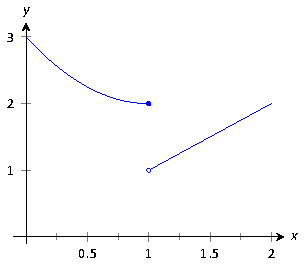
\includegraphics{test-figure2.pdf}
%  \captionof{figure}{Test caption}
%  \end{minipage}}}


%\newenvironment{mfigurefile}[2]{%
%\begin{tikzpicture}[remember picture,overlay]%
%\ifthenelse{\isodd{\thepage}}{\node [xshift=-36pt-.5\marginparwidth,yshift=#2\paperheight] at (current page.south east) }{\node [xshift=36pt+.5\marginparwidth,yshift=#2\paperheight] at (current page.south west) }%
%{\input{#1}};}%
%{\end{tikzpicture}%
%}

%\DeclareCaptionType{mytype}[Typename][List of mytype]


    
%%%%
%% End margin figure 
%%%%    
    

\newcommand{\bmx}[1]{\left[\hskip -3pt\begin{array}{#1} }
\newcommand{\emx}{\end{array}\hskip -3pt\right]}

\newcommand{\btz}{\begin{center}\begin{tikzpicture}}
\newcommand{\etz}{\end{tikzpicture}\end{center}}

\newcommand{\ds}{\displaystyle}

\newcommand{\fp}{\ensuremath{f\,'}}
\newcommand{\fpp}{\ensuremath{f\,''}}

\newcommand{\Fp}{\ensuremath{F\primeskip'}}
\newcommand{\Fpp}{\ensuremath{F\primeskip''}}

\newcommand{\yp}{\ensuremath{y\primeskip'}}
\newcommand{\gp}{\ensuremath{g\primeskip'}}

\newcommand{\dx}{\ensuremath{\Delta x}}
\newcommand{\dy}{\ensuremath{\Delta y}}
%\newcommand{\dz}{\ensuremath{\Delta z}}
\newcommand{\ddz}{\ensuremath{\Delta z}}

\newcommand{\thet}{\ensuremath{\theta}}
\newcommand{\norm}[1]{\ensuremath{||\ #1\ ||}}
\newcommand{\vnorm}[1]{\ensuremath{\norm{\vec #1}}}
\newcommand{\snorm}[1]{\ensuremath{\left|\left|\ #1\ \right|\right|}}
\newcommand{\la}{\left\langle}
\newcommand{\ra}{\right\rangle}
\newcommand{\dotp}[2]{\ensuremath{\vec #1 \cdot \vec #2}}
\newcommand{\proj}[2]{\ensuremath{\text{proj}_{\,\vec #2}{\,\vec #1}}}
\newcommand{\crossp}[2]{\ensuremath{\vec #1 \times \vec #2}}
\newcommand{\veci}{\ensuremath{\vec i}}
\newcommand{\vecj}{\ensuremath{\vec j}}
\newcommand{\veck}{\ensuremath{\vec k}}
\newcommand{\vecu}{\ensuremath{\vec u}}
\newcommand{\vecv}{\ensuremath{\vec v}}
\newcommand{\vecw}{\ensuremath{\vec w}}
\newcommand{\vecx}{\ensuremath{\vec x}}
\newcommand{\vecy}{\ensuremath{\vec y}}
\newcommand{\vrp}{\ensuremath{\vec r\, '}}
\newcommand{\vsp}{\ensuremath{\vec s\, '}}
\newcommand{\vrt}{\ensuremath{\vec r(t)}}
\newcommand{\vst}{\ensuremath{\vec s(t)}}
\newcommand{\vvt}{\ensuremath{\vec v(t)}}
\newcommand{\vat}{\ensuremath{\vec a(t)}}
\newcommand{\px}{\ensuremath{\partial x}}
\newcommand{\py}{\ensuremath{\partial y}}
\newcommand{\pz}{\ensuremath{\partial z}}
\newcommand{\pf}{\ensuremath{\partial f}}
\newcommand{\underlinespace}{\underline{\phantom{xxxxxx}}}

\newcommand{\surfaceS}{\ensuremath{\mathcal{S}}}

\newcommand{\mathN}{\ensuremath{\mathbb{N}}}

\newcommand{\zerooverzero}{\ensuremath{\ds \raisebox{8pt}{\text{``\ }}\frac{0}{0}\raisebox{8pt}{\text{\ ''}}}}


\newcommand{\myrule}{\rule[-4pt]{0pt}{13pt}}
\newcommand{\mmrule}{\rule[-10pt]{0pt}{15pt}}
\newcommand{\myds}{\ds\mmrule}
\newcommand{\deriv}[2]{\ensuremath{\myds\frac{d}{dx}\left(#1\right)=#2}}
\newcommand{\myint}[2]{\ensuremath{\myds\int #1\ dx=} \ensuremath{\ds #2}}

\DeclareMathOperator{\sech}{sech}
\DeclareMathOperator{\csch}{csch}
\DeclareMathOperator{\curl}{curl}
\DeclareMathOperator{\divv}{div}

\newcommand{\sword}[1]{\textbf{#1}}

\newcommand{\primeskip}{\hskip.75pt}

%%%% Begin Header TikZ

%  Some TiKZ  shortcuts to help make drawing 3D vectors faster.
%

\newcommand{\plotlinecolor}{blue}

%
% Draw x and y tick marks
%
\newcommand{\drawxticks}[1]
{\foreach \x in {#1}
		{\draw  (\x,-.1)--(\x,.1);
			};
}
\newcommand{\drawyticks}[1]
{\foreach \x in {#1}
		{\draw  (-.1,\x)--(.1,\x);
			};
}

\newcommand{\drawxlines}[3]
{\draw[<->] (#1,0) -- (#2,0) node [right] {$x$};
\foreach \x in {#3}
		{\draw  (\x,-.1)--(\x,.1);
			};
}

\newcommand{\drawylines}[3]
{\draw[<->] (0,#1) -- (0,#2) node [above] {$y$};
\foreach \x in {#3}
		{\draw  (-.1,\x)--(.1,\x);
			};
}

\newcommand{\drawxlabels}[1]
{\foreach \x in {#1}
		{\draw  (\x,-.1) node [below] {\scriptsize $\x$};
		};
}

\newcommand{\drawylabels}[1]
{\foreach \x in {#1}
		{\draw  (-.1,\x) node [left] {\scriptsize $\x$};
		};
}

%% draw a box of margin width size to see if figure is properly contained within
\newcommand{\marginsizebox}{\draw (0,0)--(\marginparwidth,0)--(\marginparwidth,3)--(0,3)--cycle;}

%%%%
%%%%

\newcommand{\asyouread}[1]{\begin{tikzpicture}
\ifthenelse{\boolean{in_color}}{\node [preaction={fill=black,opacity=.5,transform canvas={xshift=1mm,yshift=-1mm}}, right color=blue!80!black!30, left color=blue!80] at (0,0) {\textcolor{white}{\textsf{\textit{AS YOU READ $\ldots$}}}};}
{\node [preaction={fill=black,opacity=.5,transform canvas={xshift=1mm,yshift=-1mm}}, right color=black!30, left color=black!10] at (0,0) {\textcolor{white}{\textsf{\textit{AS YOU READ $\ldots$}}}};}
\end{tikzpicture}
\begin{enumerate}
#1
\end{enumerate}
\vskip 20pt}

%%%%
%%  A new figure environment, trying to fix the float problem.
%%
%%%%

%\newcounter{myfigurecounter}[chapter]
%\renewcommand\themyfigurecounter{\thechapter.\arabic{myfigurecounter}}
%\newenvironment{myfigure}{\refstepcounter{myfigurecounter}}{}
%\newcommand{\mycaption}[1]{%
%\begin{center}%
%\vskip -1.5\baselineskip
%\begin{tikzpicture}%
%\draw (0,0) node [text width=\textwidth,align=center] {Figure \themyfigurecounter: #1};%
%\end{tikzpicture}%
%\end{center}%
%}
\usepackage{pgfplots}
\pgfplotsset{compat=1.8}
\usepackage{pdfpages}



\ifthenelse{\boolean{xetex}}%
	{\sffamily
	%%\usepackage{fontspec}
	\usepackage{mathspec}
	\setallmainfonts[Mapping=tex-text]{Calibri}
	\setmainfont[Mapping=tex-text]{Calibri}
	\setsansfont[Mapping=tex-text]{Calibri}
	\setmathsfont(Greek){[cmmi10]}}
	{}
	
	\ifthenelse{\boolean{luatex}}%
	{\sffamily
	\usepackage{fontspec}
	\usepackage{unicode-math}
	%\usepackage{mathspec}
	%\setallmainfonts[Mapping=tex-text]{Calibri}
	\setmainfont{Calibri}
	%\setsansfont[Mapping=tex-text]{Calibri}
	\setmathfont[range=\mathup]{Calibri}
	\setmathfont[range=\mathit]{Calibri Italic}
	}
	{}

\makeindex

%%%\tracingonline=1
\begin{document}
\printexercisenames
\printincolor
%\printinblackandwhite
\printallanswers


%%%
%%%%%%%%%%
%%%
%%%  Set criteria for the format of the book.
%%%  This supercedes anything set in the Text_Header.
%%%
%%%%%%%%%%



%\printinblackandwhite

%\printexercisenames

%\nodrawexamplelines

%\printallanswers


\normalem



%%%\pagenumbering{roman}

%%%%%%
%%%		For editing purposes, block comment down to 
%%%		the next mark
%%%%%%

%%%%\input{cover/front_cover_in_text}
%%%%\clearpage
%%%%\thispagestyle{empty}
\frontmatter
%%%%
%%%%\title{\textsc{Fundamentals of Matrix Algebra}\\
%%%%{\small Version 2.1011}}
%%%%\author{Gregory N. Hartman, Ph.D.}
%%%%\date{}

\vspace*{\stretch{.5}}

\hskip 125pt\begin{minipage}{\textwidth}
\begin{flushright}

\textsc{\large \apex\ {\Huge Calculus I}} \\

%\textsl{Third Edition}, 
{\small Version 3.0}\\

\Large
\vspace{1in}

Gregory Hartman, Ph.D.

\emph{\small Department of Applied Mathematics}

\emph{\small Virginia Military Institute}\vskip15pt

\parbox{200pt}{\textit{Contributing Authors}}\hskip 2cm \phantom{.}

Troy Siemers, Ph.D.

\emph{\small Department of Applied Mathematics}

\emph{\small Virginia Military Institute}\vskip 15pt

Brian Heinold, Ph.D.

\emph{\small Department of Mathematics and Computer Science}

\emph{\small Mount Saint Mary's University}\vskip 15pt

Dimplekumar Chalishajar, Ph.D.

\emph{\small Department of Applied Mathematics}

\emph{\small Virginia Military Institute}\vskip 25pt

\parbox{200pt}{\textit{Editor}}\hskip 2cm \phantom{.}
%\textit{Editor}\hskip 7cm\phantom{.}

Jennifer Bowen, Ph.D.

\emph{\small Department of Mathematics and Computer Science}

\emph{\small The College of Wooster}

\normalsize
\end{flushright}
\end{minipage}

\vspace{\stretch{1}}


\thispagestyle{empty}
\clearpage

\vspace*{\stretch{5}}
\noindent\hskip -1in\begin{minipage}{2in}

\includegraphics{text/by-nc} 
\end{minipage}
\begin{minipage}{3in}
\noindent Copyright \copyright\ 2015 Gregory Hartman

Licensed to the public under Creative Commons Attribution-Noncommercial 4.0 International Public License
\end{minipage}

\vspace{\stretch{1}} 
\thispagestyle{empty}
\clearpage
%
%
%\cleardoublepage
%%%%\phantomsection
%%%%\input{text/thanks}
%%%%\addcontentsline{toc}{chapter}{Thanks} 
%%%%\clearpage{\pagestyle{empty}\cleardoublepage}
%%%%\phantomsection
%%%%\thispagestyle{empty}
\Huge
\noindent {\bf \textsc{Preface}}\\
\large
\emph{A Note on Using this Text}
\vspace{1in}
\normalsize

Thank you for reading this short preface. Allow us to share a few key points about the text so that you may better understand what you will find beyond this page.

This text comprises a three--volume series on Calculus. The first part covers material taught in many ``Calc 1'' courses: limits, derivatives, and the basics of integration, found in Chapters 1 through 6.1. The second text covers material often taught in ``Calc 2:'' integration and its applications, along with an introduction to sequences, series and Taylor Polynomials, found in Chapters 5 through 8. The third text covers topics common in ``Calc 3'' or ``multivariable calc:'' parametric equations, polar coordinates, vector--valued functions, and functions of more than one variable, found in Chapters 9 through 13. All three are available separately for free at \texttt{\href{http://apexcalculus.com}{www.apexcalculus.com}}. %These three texts are intended to work together and make one cohesive text, \textit{APEX Calculus}, which can also be downloaded from the website. 

Printing the entire text as one volume makes for a large, heavy, cumbersome book. One can certainly only print the pages they currently need, but some prefer to have a nice, bound copy of the text. Therefore this text has been split into these three manageable parts, each of which can be purchased for under \$15 at \href{http://amazon.com}{Amazon.com}.\\ 



%A result of this splitting is that sometimes a concept is said to be explored in a ``later section,'' though that section does not actually appear in this particular text. Downloading the .pdf of \textit{APEX Calculus} will ensure that you have all the content.  
%material is referenced that is not contained in the present text. The context should make it clear whether the ``missing'' material is in the \textit{Calculus I} or \textit{Calculus III} portion. Downloading the appropriate .pdf, or the whole \textit{APEX Calculus} .pdf, will give access to these topics.
% This splitting of the material also results in unfortunate page/chapter numberings. Chapter 5 of this text is Chapter 1 of \textit{Calculus II}. Apart from these numberings, page--for--page the content of the sections that appear in both \textit{Calculus I} and \textit{Calculus II} are identical.\\ %For instance, in this text, ``Theorem 20'' may be mentioned, although Theorem 20 is only presented in Part I. To minimize confusion, theorems, definitions and key ideas are referenced by their title or subject matter, not their number.

%The current publisher of this text does not allow one text to be split across multiple volumes, with continuity of chapters and page numberings. This is the one drawback of the current publishing model that has many advantages, highlighted below. Because of this, there are a few peculiarities 

\noindent\textbf{\large For Students: How to Read this Text}\\

Mathematics textbooks have a reputation for being hard to read. High--level mathematical writing often seeks to say much with few words, and this style often seeps into texts of lower--level topics. This book was written with the goal of being easier to read than many other calculus textbooks, without becoming too verbose. 

Each chapter and section starts with an introduction of the coming material, hopefully setting the stage for ``why you should care,'' and ends with a look ahead to see how the just--learned material helps address future problems. 

\textit{Please read the text;} it is written to explain the concepts of Calculus. There are numerous examples to demonstrate the meaning of definitions, the truth of theorems, and the application of mathematical techniques. When you encounter a sentence you don't understand, read it again. If it still doesn't make sense, read on anyway, as sometimes confusing sentences are explained by later sentences.

\textit{You don't have to read every equation.} The examples generally show ``all'' the steps needed to solve a problem. Sometimes reading through each step is helpful; sometimes it is confusing. When the steps are illustrating a new technique, one probably should follow each step closely to learn the new technique. When the steps are showing the mathematics needed to find a number to be used later, one can usually skip ahead and see how that number is being used, instead of getting bogged down in reading how the number was found.

\textit{Most proofs have been omitted.} In mathematics, \textit{proving} something is always true is extremely important, and entails much more than testing to see if it works twice. However, students often are confused by the details of a proof, or become concerned that they should have been able to construct this proof on their own. To alleviate this potential problem, we do not include the proofs to most theorems in the text. The interested reader is highly encouraged to find proofs online or from their instructor. In most cases, one is very capable of understanding what a theorem \textit{means} and \textit{how to apply it} without knowing fully \textit{why} it is true.
\\

\thispagestyle{empty}
\noindent\textbf{\large Interactive, 3D Graphics}\\

New to Version 3.0 is the addition of interactive, 3D graphics in the .pdf version. Nearly all graphs of objects in space can be rotated, shifted, and zoomed in/out so the reader can better understand the object illustrated. 

As of this writing, the only pdf viewers that support these 3D graphics are Adobe Reader \& Acrobat (and only the versions for PC/Mac/Unix/Linux computers, not tablets or smartphones). To activate the interactive mode, click on the image. Once activated, one can click/drag to rotate the object and use the scroll wheel on a mouse to zoom in/out. (A great way to investigate an image is to first zoom in on the page of the pdf viewer so the graphic itself takes up much of the screen, then zoom inside the graphic itself.) A CTRL-click/drag pans the object left/right or up/down. By right-clicking on the graph one can access a menu of other options, such as changing the lighting scheme or perspective. One can also revert the graph back to its default view. If you wish to deactive the interactivity, one can right-click and choose the ``Disable Content'' option. \\

\noindent\textbf{\large Thanks}\\

There are many people who deserve recognition for the important role they have played in the development of this text. First, I thank Michelle for her support and encouragement, even as this ``project from work'' occupied my time and attention at home. Many thanks to Troy Siemers, whose most important contributions extend far beyond the sections he wrote or the 227 figures he coded in Asymptote for 3D interaction.  He provided incredible support, advice and encouragement for which I am very grateful. My thanks to Brian Heinold and Dimplekumar Chalishajar for their contributions and to Jennifer Bowen for reading through so much material and providing great feedback early on. Thanks to Troy, Lee Dewald, Dan Joseph, Meagan Herald, Bill Lowe, John David, Vonda Walsh, Geoff Cox, Jessica Libertini and other faculty of VMI who have given me numerous suggestions and corrections based on their experience with teaching from the text. (Special thanks to Troy, Lee \& Dan for their patience in teaching Calc III while I was still writing the Calc III material.) Thanks to Randy Cone for encouraging his tutors of VMI's Open Math Lab to read through the text and check the solutions, and thanks to the tutors for spending their time doing so. A very special thanks to Kristi Brown and Paul Janiczek who took this opportunity far above \& beyond what I expected, meticulously checking every solution and carefully reading every example. Their comments have been extraordinarily helpful. I am also thankful for the support provided by Wane Schneiter, who as my Dean provided me with extra time to work on this project. I am blessed to have so many people give of their time to make this book better.\\

\noindent\textbf{\large \apex\  -- Affordable Print and Electronic teXts}\\

\apex\ is a consortium of authors  who collaborate to produce high--quality, low--cost textbooks. The current textbook--writing paradigm is facing a potential revolution as desktop publishing and electronic formats increase in popularity. However, writing a good textbook is no easy task, as the time requirements alone are substantial. It takes countless hours of work to produce text, write examples and exercises, edit and publish. Through collaboration, however, the cost to any individual can be lessened, allowing us to create texts that we freely distribute electronically and sell in printed form for an incredibly low cost. Having said that, nothing is entirely free; someone always bears some cost. This text ``cost'' the authors of this book their time, and that was not enough. \textit{APEX Calculus} would not exist had not the Virginia Military Institute, through a generous Jackson--Hope grant, given the lead author significant time away from teaching so he could focus on this text.

Each text is available as a free .pdf, protected by a Creative Commons Attribution - Noncommercial 4.0 copyright. That  means you can give the .pdf to anyone you like, print it in any form you like, and even edit the original content and redistribute it. If you do the latter, you must  clearly reference this work and you cannot sell your edited work for money.

We encourage others to adapt this work to fit their own needs. One might add sections that are ``missing'' or remove sections that your students won't need. The source files can be found at \texttt{\href{https://github.com/APEXCalculus}{github.com/APEXCalculus}}.

You can learn more at \texttt{\href{http://www.vmi.edu/APEX}{www.vmi.edu/APEX}}.
\thispagestyle{empty}


%%%%\addcontentsline{toc}{chapter}{Preface}
%%%%\clearpage{\pagestyle{empty}\cleardoublepage}
%%%%\phantomsection
%
% The following is the correct TOC; the 
%
%%%%

\addtocontents{toc}{\protect\thispagestyle{empty}}
\addcontentsline{toc}{chapter}{Table of Contents}
\tableofcontents
\clearpage{\pagestyle{empty}\cleardoublepage}

\phantomsection
\prefacegeometry
\addcontentsline{toc}{chapter}{Preface}
\thispagestyle{empty}
\Huge
\noindent {\bf \textsc{Preface}}\\
\large
\emph{A Note on Using this Text}
\vskip2\baselineskip
\normalsize

Thank you for reading this short preface. Allow us to share a few key points about the text so that you may better understand what you will find beyond this page.

This text is Part I of a three--text series on Calculus. The first part covers material taught in many ``Calc 1'' courses: limits, derivatives, and the basics of integration, found in Chapters 1 through 6.1. The second text covers material often taught in ``Calc 2:'' integration and its applications, along with an introduction to sequences, series and Taylor Polynomials, found in Chapters 5 through 8. The third text covers topics common in ``Calc 3'' or ``multivariable calc:'' parametric equations, polar coordinates, vector--valued functions, and functions of more than one variable, found in Chapters 9 through 13. All three are available separately for free at \texttt{\href{http://apexcalculus.com}{www.apexcalculus.com}}. These three texts are intended to work together and make one cohesive text, \textit{APEX Calculus}, which can also be downloaded from the website. 

Printing the entire text as one volume makes for a large, heavy, cumbersome book. One can certainly only print the pages they currently need, but some prefer to have a nice, bound copy of the text. Therefore this text has been split into these three manageable parts, each of which can be purchased for under \$15 at \href{http://amazon.com}{Amazon.com}. 

A result of this splitting is that sometimes a concept is said to be explored in a ``later section,'' though that section does not actually appear in this particular text. Also, the index makes reference to topics and page numbers that do not appear in this text. This is done intentionally to show the reader what topics are available for study.  Downloading the .pdf of \textit{APEX Calculus} will ensure that you have all the content.\\ 
%material is referenced that is not contained in the present text. The context should make it clear whether the ``missing'' material is in the \textit{Calculus I} or \textit{Calculus III} portion. Downloading the appropriate .pdf, or the whole \textit{APEX Calculus} .pdf, will give access to these topics.
  %For instance, in this text, ``Theorem 20'' may be mentioned, although Theorem 20 is only presented in Part I. To minimize confusion, theorems, definitions and key ideas are referenced by their title or subject matter, not their number.

%The current publisher of this text does not allow one text to be split across multiple volumes, with continuity of chapters and page numberings. This is the one drawback of the current publishing model that has many advantages, highlighted below. Because of this, there are a few peculiarities 

\noindent\textbf{\large For Students: How to Read this Text}\\

Mathematics textbooks have a reputation for being hard to read. High--level mathematical writing often seeks to say much with few words, and this style often seeps into texts of lower--level topics. This book was written with the goal of being easier to read than many other calculus textbooks, without becoming too verbose. 

Each chapter and section starts with an introduction of the coming material, hopefully setting the stage for ``why you should care,'' and ends with a look ahead to see how the just--learned material helps address future problems. 

\textit{Please read the text;} it is written to explain the concepts of Calculus. There are numerous examples to demonstrate the meaning of definitions, the truth of theorems, and the application of mathematical techniques. When you encounter a sentence you don't understand, read it again. If it still doesn't make sense, read on anyway, as sometimes confusing sentences are explained by later sentences.

\textit{You don't have to read every equation.} The examples generally show ``all'' the steps needed to solve a problem. Sometimes reading through each step is helpful; sometimes it is confusing. When the steps are illustrating a new technique, one probably should follow each step closely to learn the new technique. When the steps are showing the mathematics needed to find a number to be used later, one can usually skip ahead and see how that number is being used, instead of getting bogged down in reading how the number was found.

\textit{Most proofs have been omitted.} In mathematics, \textit{proving} something is always true is extremely important, and entails much more than testing to see if it works twice. However, students often are confused by the details of a proof, or become concerned that they should have been able to construct this proof on their own. To alleviate this potential problem, we do not include the proofs to most theorems in the text. The interested reader is highly encouraged to find proofs online or from their instructor. In most cases, one is very capable of understanding what a theorem \textit{means} and \textit{how to apply it} without knowing fully \textit{why} it is true.
\\

\thispagestyle{empty}
\noindent\textbf{\large Interactive, 3D Graphics}\\

New to Version 3.0 is the addition of interactive, 3D graphics in the .pdf version. Nearly all graphs of objects in space can be rotated, shifted, and zoomed in/out so the reader can better understand the object illustrated. 

As of this writing, the only pdf viewers that support these 3D graphics are Adobe Reader \& Acrobat (and only the versions for PC/Mac/Unix/Linux computers, not tablets or smartphones). To activate the interactive mode, click on the image. Once activated, one can click/drag to rotate the object and use the scroll wheel on a mouse to zoom in/out. (A great way to investigate an image is to first zoom in on the page of the pdf viewer so the graphic itself takes up much of the screen, then zoom inside the graphic itself.) A CTRL-click/drag pans the object left/right or up/down. By right-clicking on the graph one can access a menu of other options, such as changing the lighting scheme or perspective. One can also revert the graph back to its default view. If you wish to deactivate the interactivity, one can right-click and choose the ``Disable Content'' option. \\

\noindent\textbf{\large Thanks}\\

There are many people who deserve recognition for the important role they have played in the development of this text. First, I thank Michelle for her support and encouragement, even as this ``project from work'' occupied my time and attention at home. Many thanks to Troy Siemers, whose most important contributions extend far beyond the sections he wrote or the 227 figures he coded in Asymptote for 3D interaction.  He provided incredible support, advice and encouragement for which I am very grateful. My thanks to Brian Heinold and Dimplekumar Chalishajar for their contributions and to Jennifer Bowen for reading through so much material and providing great feedback early on. Thanks to Troy, Lee Dewald, Dan Joseph, Meagan Herald, Bill Lowe, John David, Vonda Walsh, Geoff Cox, Jessica Libertini and other faculty of VMI who have given me numerous suggestions and corrections based on their experience with teaching from the text. (Special thanks to Troy, Lee \& Dan for their patience in teaching Calc III while I was still writing the Calc III material.) Thanks to Randy Cone for encouraging his tutors of VMI's Open Math Lab to read through the text and check the solutions, and thanks to the tutors for spending their time doing so. A very special thanks to Kristi Brown and Paul Janiczek who took this opportunity far above \& beyond what I expected, meticulously checking every solution and carefully reading every example. Their comments have been extraordinarily helpful. I am also thankful for the support provided by Wane Schneiter, who as my Dean provided me with extra time to work on this project. I am blessed to have so many people give of their time to make this book better.\\

\clearpage
\noindent\textbf{\large \apex\  -- Affordable Print and Electronic teXts}\\

\apex\ is a consortium of authors  who collaborate to produce high--quality, low--cost textbooks. The current textbook--writing paradigm is facing a potential revolution as desktop publishing and electronic formats increase in popularity. However, writing a good textbook is no easy task, as the time requirements alone are substantial. It takes countless hours of work to produce text, write examples and exercises, edit and publish. Through collaboration, however, the cost to any individual can be lessened, allowing us to create texts that we freely distribute electronically and sell in printed form for an incredibly low cost. Having said that, nothing is entirely free; someone always bears some cost. This text ``cost'' the authors of this book their time, and that was not enough. \textit{APEX Calculus} would not exist had not the Virginia Military Institute, through a generous Jackson--Hope grant, given the lead author significant time away from teaching so he could focus on this text.

Each text is available as a free .pdf, protected by a Creative Commons Attribution - Noncommercial 4.0 copyright. That  means you can give the .pdf to anyone you like, print it in any form you like, and even edit the original content and redistribute it. If you do the latter, you must  clearly reference this work and you cannot sell your edited work for money.

We encourage others to adapt this work to fit their own needs. One might add sections that are ``missing'' or remove sections that your students won't need. The source files can be found at \texttt{\href{https://github.com/APEXCalculus}{github.com/APEXCalculus}}.

You can learn more at \texttt{\href{http://www.vmi.edu/APEX}{www.vmi.edu/APEX}}.
\thispagestyle{empty}


\restoregeometry
\clearpage{\pagestyle{empty}\cleardoublepage}

%%%%%
%\includepdf[pages={1,2}]{CalculusTOC.pdf}

%%%%
\mainmatter


%%%%
%		End block comment here
%%%%





%
%\chapter{Limits}\label{chapter:limits}
%\thispagestyle{empty}
%%%%
%\textit{Calculus} means ``a method of calculation or reasoning.'' When one computes the sales tax on a purchase, one employs a simple calculus. When one finds the area of a polygonal shape by breaking it up into a set of triangles, one is using another calculus. Proving a theorem in geometry employs yet another calculus.

Despite the wonderful advances in mathematics that had taken place into the first half of the $17^\text{th}$ century, mathematicians and scientists were keenly aware of what they \textit{could not do.} (This is true even today.) In particular, two important concepts eluded mastery by the great thinkers of that time: area and rates of change. 

Area seems innocuous enough; areas of circles, rectangles, parallelograms, etc., are standard topics of study for students today just as they were then. However, the areas of \textit{arbitrary} shapes could not be computed, even if the boundary of the shape could be described exactly. 

Rates of change were also important. When an object moves at a constant rate of change, then ``distance = rate $\times $ time.'' But what if the rate is not constant -- can distance still be computed? Or, if distance is known, can we discover the rate of change?

It turns out that these two concepts were related. Two mathematicians, Sir Isaac Newton and Gottfried Leibniz, are credited with independently formulating a system of computing that solved the above problems and showed how they were connected. Their system of reasoning was ``a'' calculus. However, as the power and importance of their discovery took hold, it became known to many as ``the'' calculus. Today, we generally shorten this to discuss ``calculus.''

The foundation of ``the calculus'' is the \textit{limit.} It is a tool to describe a particular behavior of a function. This chapter begins our study of the limit by approximating its value graphically and numerically. After a formal definition of the limit, properties are established that make ``finding limits'' tractable. Once the limit is understood, then the problems of area and rates of change can be approached.



\section{An Introduction To Limits}\label{sec:limit_intro}

We begin our study of \textit{limits} by considering examples that demonstrate key concepts that will be explained as we progress.\\

Consider the function $y = \frac{\sin x}{x}$. When $x$ is near the value 1, what value (if any) is $y$ near?%

While our question is not precisely formed (what constitutes ``near the value 1''?), the answer does not seem difficult to find. One might think first to look at a graph of this function to approximate the appropriate $y$ values. Consider Figure \ref{fig:zoom_sinx_over_x}, where $y = \frac{\sin x}{x}$ is graphed. For values of $x$ near 1, it seems that $y$ takes on values near $0.85$. In fact, when $x=1$, then $y=\frac{\sin 1}{1} \approx 0.84$, so it makes sense that when $x$ is ``near'' 1, $y$ will be ``near'' $0.84$.

\mfigure{.8}{$\sin(x)/x$ near $x=1$.}{fig:zoom_sinx_over_x}{figures/figZoomSinXOverX}
\mfigure{.55}{$\sin(x)/x$ near $x=0$.}{fig:sinx_over_x}{figures/figSinXOverX}
Consider this again at a different value for $x$. When $x$ is near 0, what value (if any) is $y$ near? By considering Figure \ref{fig:sinx_over_x}, one can see that it seems that $y$ takes on values near $1$. But what happens when $x=0$? We have $$ y \rightarrow \frac{\sin 0}{0} \rightarrow \raisebox{8pt}{\text{``\ }}\frac{0}{0}\raisebox{8pt}{\text{\ ''}}.$$ 
The expression ``$0/0$'' has no value; it is \emph{indeterminate.} \index{limit!indeterminate form}\index{indeterminate form} Such an expression gives no information about what is going on with the function nearby. We cannot find out how $y$ behaves near $x=0$ for this function simply by letting $x=0$. 

\emph{Finding a limit} entails understanding how a function behaves near a particular value of $x$. Before continuing, it will be useful to establish some notation. Let $y=f(x)$; that is, let $y$ be a function of $x$ for some function $f$. The expression ``the limit of $y$ as $x$ approaches 1'' describes a number, often referred to as $L$, that $y$ nears as $x$ nears 1. We write all this as $$\lim_{x\to 1} y = \lim_{x\to 1} f(x) = L.$$ This is not a complete definition (that will come in the next section); this is a pseudo-definition that will allow us to explore the idea of a limit. \index{limit!pseudo-definition}

Above, where $f(x) = \sin(x)/x$, we approximated $$\lim_{x\to 1} \frac{\sin x}{x} \approx 0.84 \quad \text{ and } \quad \lim_{x\to 0}\frac{\sin x}{x} \approx 1.$$ (We \textit{approximated} these limits, hence used the ``$\approx$'' symbol, since we are working with the pseudo-definition of a limit, not the actual definition.)

Once we have the true definition of a limit, we will find limits \textit{analytically}; that is, exactly using a variety of mathematical tools. For now, we will \textit{approximate} limits both graphically and numerically. Graphing a function can provide a good approximation, though often not very precise. Numerical methods can provide a more accurate approximation. We have already approximated limits graphically, so we now turn our attention to numerical approximations.


Consider again $\lim_{x\to 1}\sin (x)/x$. To approximate this limit numerically, we can create a table of $x$ and $f(x)$ values where $x$ is ``near'' 1. This is done in Figure \ref{table:sinx_1}.\par

Notice that for values of $x$ near $1$, we have $\sin (x)/x$ near $0.841$. The $x=1$ row is in bold to highlight the fact that when considering limits, we are \textit{not} concerned with the value of the function at that particular $x$ value; we are only concerned with the values of the function when $x$ is \textit{near} 1. 

\mtable{.3}{Values of $\sin(x)/x$ with $x$ near 1.}{table:sinx_1}{\begin{tabular}{cc}
$x$ & $\sin(x)/x$ \\ \hline 
0.9 & 0.870363 \\
 0.99 & 0.844471 \\
 0.999 & 0.841772 \\
 \textbf{1} & \textbf{0.841471} \\
 1.001 & 0.84117 \\
 1.01 & 0.838447 \\
 1.1 & 0.810189
\end{tabular}
%\caption{Values of $\frac{\sin x}{x}$ for $x$ near 1.}\label{fig:sinx_1_table}
}

%\vskip \baselineskip

Now approximate $\lim_{x\to 0} \sin(x)/x$ numerically. We already approximated the value of this limit as 1 graphically in Figure \ref{fig:sinx_over_x}. The table in Figure \ref{table:sinx_2} shows the value of $\sin(x)/x$ for values of $x$ near 0. Ten places after the decimal point are shown to highlight how close to 1 the value of $\sin(x)/x$ gets as $x$ takes on values very near 0. We include the $x=0$ row in bold again to stress that we are not concerned with the value of our function at $x=0$, only on the behavior of the function \textit{near} 0. 

\mtable{.8}{Values of $\sin(x)/x$ with $x$ near 0.}{table:sinx_2}{\begin{tabular}{cc}
$x$ & $\sin(x)/x$ \\ \hline
 -0.1 & 0.9983341665 \\
 -0.01 & 0.9999833334 \\
 -0.001 & 0.9999998333 \\
 \textbf{0} & \textbf{not defined} \\
 0.001 & 0.9999998333 \\
 0.01 & 0.9999833334 \\
 0.1 & 0.9983341665
 \end{tabular}
% \caption{Values of $\frac{\sin x}{x}$ for $x$ near 0.}\label{fig:sinx_0_table}}
 
This numerical method gives confidence to say that 1 is a good approximation of $\lim_{x\to 0} \sin(x)/x$; that is, $$\lim_{x\to 0} \sin(x)/x \approx 1.$$ Later we will be able to prove that the limit is \textit{exactly} 1.

We now consider several examples that allow us explore different aspects of the limit concept.\\

\mfigure{.55}{Graphically approximating a limit in Example \ref{ex_limit1}.}{fig:limit1}{figures/figlimit1}
\mtable{.35}{Numerically approximating a limit in Example \ref{ex_limit1}.}{table:limit1}{\begin{tabular}{cc}
$x$ & $\frac{x^2-x-6}{6x^2-19x+3}$ \\ \hline
2.9 & 0.29878 \\
 2.99 & 0.294569 \\
 2.999 & 0.294163 \\
 \textbf{3} & \textbf{not defined}\\
 3.001 & 0.294073 \\
 3.01 & 0.293669 \\
 3.1 & 0.289773
 \end{tabular}
}

\example{ex_limit1}{Approximating the value of a limit}{
Use graphical and numerical methods to approximate $$\lim_{x\to 3} \frac{x^2-x-6}{6x^2-19x+3}.$$}%
{To graphically approximate the limit, graph $$y = (x^2-x-6)/(6x^2-19x+3)$$ on a small interval that contains 3. To numerically approximate the limit, create a table of values where the $x$ values are near 3. This is done in Figures \ref{fig:limit1} and \ref{table:limit1}, respectively.

\enlargethispage{2\baselineskip}

The graph shows that when $x$ is near 3, the value of $y$ is very near $0.3$. By considering values of $x$ near 3, we see that $y=0.294$ is a better approximation. The graph and the table imply that $$\lim_{x\to 3} \frac{x^2-x-6}{6x^2-19x+3} \approx 0.294.$$ 
\vskip -\baselineskip
}\\

This example may bring up a few questions about approximating limits (and the nature of limits themselves). 
\begin{enumerate}
\item		If a graph does not produce as good an approximation as a table, why bother with it?
\item		How many values of $x$ in a table are ``enough?'' In the previous example, could we have just used $x=3.001$ and found a fine approximation?
\end{enumerate}

Graphs are useful since they give a visual understanding concerning the behavior of a function. Sometimes a function may act ``erratically'' near certain $x$ values which is hard to discern numerically but very plain graphically. Since graphing utilities are very accessible, it makes sense to make proper use of them.


Since tables and graphs are used only to \textit{approximate} the value of a limit, there is not a firm answer to how many data points are ``enough.'' Include enough so that a trend is clear, and use values (when possible) both less than and greater than the value in question. In Example \ref{ex_limit1}, we used both values less than and greater than 3. Had we used just $x=3.001$, we might have been tempted to conclude that the limit had a value of $0.3$. While this is not far off, we could do better. Using values ``on both sides of 3'' helps us identify trends.\\

\example{ex_limit2}{Approximating the value of a limit}{
Graphically and numerically approximate the limit of $f(x)$ as $x$ approaches 0, where $$f(x) = \left\{\begin{array}{rl} x+1 & x< 0 \\ -x^2+1 & x > 0 \end{array}\right..$$}{Again we graph $f(x)$ and create a table of its values near $x=0$ to approximate the limit. Note that this is a piecewise defined function, so it behaves differently on either side of 0. Figure \ref{fig:limit2} shows a graph of $f(x)$, and on either side of 0 it seems the $y$ values approach 1. Note that $f(0)$ is not actually defined, as indicated in the graph with the open circle.

\mfigure{.65}{Graphically approximating a limit in Example \ref{ex_limit2}.}{fig:limit2}{figures/figlimit2}
\mtable{.45}{Numerically approximating a limit in Example \ref{ex_limit2}.}{table:limit2}{\begin{tabular}{cc}
$x$ & $f(x)$ \\ \hline
-0.1 & 0.9 \\
 -0.01 & 0.99 \\
 -0.001 & 0.999 \\
 0.001 & 0.999999 \\
 0.01 & 0.9999 \\
 0.1 & 0.99
 \end{tabular}
}

The table shown in Figure \ref{table:limit2} shows values of $f(x)$ for values of $x$ near 0. It is clear that as $x$ takes on values very near 0, $f(x)$ takes on values very near 1. It turns out that if we let $x=0$ for either ``piece'' of $f(x)$, 1 is returned; this is significant and we'll return to this idea later.

The graph and table allow us to say that $\lim_{x\to 0}f(x) \approx 1$; in fact, we are probably very sure it \emph{equals} 1.
}\\

\enlargethispage{\baselineskip}
\vskip \baselineskip
\noindent\textbf{\large Identifying When Limits Do Not Exist}\\

A function may not have a limit for all values of $x$. That is, we cannot say $\lim_{x\to c}f(x)=L$ for some numbers $L$ for all values of $c$, for there may not be a number that $f(x)$ is approaching. There are three common ways in which a limit may fail to exist. \index{limit!does not exist}
\begin{enumerate}
\item		The function $f(x)$ may approach different values on either side of $c$.
\item		The function may grow without upper or lower bound as $x$ approaches $c$.
\item		The function may oscillate as $x$ approaches $c$ without approaching a specific value.
\end{enumerate}

We'll explore each of these in turn.\\

\vskip \baselineskip

%\noindent
%

\example{ex_no_limit1}{Different Values Approached From Left and Right}{
Explore why $\ds\lim_{x\to 1} f(x)$ does not exist, where $$f(x) = \left\{\begin{array}{cl} x^2-2x+3 & x\leq 1 \\ x & x>1 \end{array}\right..$$}%
{
A graph of $f(x)$ around $x=1$ and a table are given in Figures \ref{fig:nolimit1} and \ref{table:nolimit1}, respectively. It is clear that as $x$ approaches 1, $f(x)$ does not seem to approach a single number. Instead, it seems as though $f(x)$ approaches two different numbers. When considering values of $x$ less than 1 (approaching 1 from the left), it seems that $f(x)$ is approaching 2; when considering values of $x$ greater than 1 (approaching 1 from the right), it seems that $f(x)$ is approaching 1. Recognizing this behavior is important; we'll study this in greater depth later. Right now, it suffices to say that the limit does not exist since $f(x)$ is not approaching one value as $x$ approaches 1.
\mfigure{.8}{Observing no limit as $x\to 1$ in Example \ref{ex_no_limit1}.}{fig:nolimit1}{figures/fignolimit1}
\mtable{.6}{Values of $f(x)$ near $x=1$ in Example \ref{ex_no_limit1}.}{table:nolimit1}{\begin{tabular}{cc}
$x$ & $f(x)$ \\ \hline
 0.9 & 2.01 \\
 0.99 & 2.0001 \\
 0.999 & 2.000001 \\
 1.001 & 1.001 \\
 1.01 & 1.01 \\
 1.1 & 1.1
\end{tabular}
}
}\\

%
%\vskip \baselineskip
%\noindent\textbf{The Function Grows Without Bound}\\

%\begin{tikzpicture}
\begin{axis}[width=\marginparwidth+25pt,tick label style={font=\scriptsize},minor x tick num=1,axis y line=middle,axis x line=middle,ymin=-1,ymax=110,xmin=-.1,xmax=2.1,name=myplot]

\addplot [{\colorone},smooth,thick] coordinates {(0.,1.) (0.05,1.10803) (0.1,1.23457) (0.15,1.38408) (0.2,1.5625)(0.25,1.77778) (0.3,2.04082) (0.35,2.36686) (0.4,2.77778)(0.45,3.30579) (0.5,4.) (0.55,4.93827) (0.6,6.25) (0.65,8.16327)(0.7,11.1111) (0.75,16.) (0.8,25.) (0.85,44.4444) (0.9,100.) };
\addplot [{\colorone},smooth,thick] coordinates {(1.1,100.) (1.15,44.4444) (1.2,25.) (1.25,16.) (1.3,11.1111) (1.35,8.16327) (1.4,6.25) (1.45,4.93827) (1.5,4.) (1.55,3.30579) (1.6,2.77778) (1.65,2.36686) (1.7,2.04082) (1.75,1.77778) (1.8,1.5625) (1.85,1.38408) (1.9,1.23457) (1.95,1.10803) (2.,1.)};
%\addplot [{\colorone},smooth] coordinates {(1,1) (1.1,1.1) (1.2,1.2) (1.3,1.3) (1.4,1.4) (1.5,1.5) (1.6,1.6) (1.7,1.7) (1.8,1.8) (1.9,1.9) (2.,2.)
\draw [dashed,thick] (axis cs: 1,1) -- (axis cs: 1,100);
\end{axis}
\node [right] at (myplot.right of origin) {\scriptsize $x$};
\node [above] at (myplot.above origin) {\scriptsize $y$};
\end{tikzpicture}
%\caption{of $f(x)$ in Example \ref{ex_no_limit2}.}\label{fig:nolimit2}
\example{ex_no_limit2}{The Function Grows Without Bound}{
Explore why $\ds\lim_{x\to 1} 1/(x-1)^2$ does not exist.}%
{A graph and table of $f(x) = 1/(x-1)^2$ are given in Figures \ref{fig:nolimit2} and \ref{table:nolimit2}, respectively. Both show that as $x$ approaches 1, $f(x)$ grows larger and larger. 
\mfigure{.4}{Observing no limit as $x\to 1$ in Example \ref{ex_no_limit2}.}{fig:nolimit2}{figures/fignolimit2}
\mtable{.2}{Values of $f(x)$ near $x=1$ in Example \ref{ex_no_limit2}.}{table:nolimit2}{\begin{tabular}{cc}
$x$ & $f(x)$ \\ \hline
 0.9 & 100. \\
 0.99 & 10000. \\
 0.999 & $1.\times 10^6$ \\
 1.001 & $1.\times 10^6$ \\
 1.01 & 10000. \\
 1.1 & 100.
\end{tabular}}

We can deduce this on our own, without the aid of the graph and table. If $x$ is near 1, then $(x-1)^2$ is very small, and: $$\frac{1}{\text{very small number}} = \text{very large number}.$$
Since $f(x)$ is not approaching a single number, we conclude that $$\lim_{x\to 1}\frac{1}{(x-1)^2}$$ does not exist.
}\\

%\vskip \baselineskip
%\noindent\textbf{The Function Oscillates}\\

\example{ex_no_limit3}{The Function Oscillates}{
Explore why $\ds\lim_{x\to 0}\sin(1/x)$ does not exist.}%
{%\mfigure{.4}{Observing no limit as $x\to 0$ in Example \ref{ex_no_limit3}.}{fig:nolimit3a}{figures/figNoLimit3a}
%\mfigure{.2}{Zooming in to observing no limit as $x\to 0$ in Example \ref{ex_no_limit3}.}{fig:nolimit3b}{figures/figNoLimit3b}
Two graphs of $f(x) = \sin(1/x)$ are given in Figures \ref{fig:nolimit3}. Figure \ref{fig:nolimit3}(a) shows $f(x)$ on the interval $[-1,1]$; notice how $f(x)$ seems to oscillate near $x=0$. One might think that despite the oscillation, as $x$ approaches 0, $f(x)$ approaches 0. However, Figure \ref{fig:nolimit3}(b) zooms in on $\sin(1/x)$, on the interval $[-0.1,0.1]$. Here the oscillation is even more pronounced. Finally, in the table in Figure \ref{fig:nolimit3}(c), we see $\sin(x)/x$ evaluated for values of $x$ near 0. As $x$ approaches 0, $f(x)$ does not appear to approach any value. 

It can be shown that in reality, as $x$ approaches 0, $\sin(1/x)$ takes on all values between $-1$ and 1 infinite times! Because of this oscillation,

 $\ds\lim_{x\to 0}\sin(1/x)$ does not exist.}\\

\ifthenelse{\boolean{longpage}}%%% if longpage, squeeze it in
{\vskip\baselineskip
\noindent\begin{minipage}{\textwidth}\centering
\begin{tabular}{cc}
(a) \myincludegraphics[scale=.9]{figures/figNoLimit3a} & (b) \myincludegraphics[scale=.9]{figures/figNoLimit3b}\end{tabular}
\vskip \baselineskip
\begin{tabular}{c}
(c)\begin{tabular}[b]{cc}
 $x$ & $\sin(1/x)$ \\ \hline 0.1 & $-0.544021$ \\ 0.01 & $-0.506366$ \\ 0.001 & 0.82688 \\ 0.0001 & $-0.305614$ \\ $1.\times 10^{-5}$ & 0.0357488 \\
 $1.\times 10^{-6}$ & $-0.349994$ \\ $1.\times 10^{-7}$ & 0.420548 \\ \\\end{tabular}\end{tabular}%
\captionsetup{type=figure}%
\caption{Observing that $f(x) = \sin(1/x)$ has no limit as $x\to 0$ in Example \ref{ex_no_limit3}.}\label{fig:nolimit3}
\end{minipage}} %% else, not longpage

%\vskip 1\baselineskip
\ifthenelse{\isodd{\thepage}}{}{\noindent\hskip -\marginparwidth }
\noindent\begin{minipage}{\textwidth+\marginparwidth+\marginparsep}%\centering
\begin{tabular}{ccc}
\myincludegraphics{figures/figNoLimit3a} &  \myincludegraphics{figures/figNoLimit3b} &  \begin{tabular}[b]{cc}
 $x$ & $\sin(1/x)$ \\ \hline 0.1 & $-0.544021$ \\ 0.01 & $-0.506366$ \\ 0.001 & 0.82688 \\ 0.0001 & $-0.305614$ \\ $1.\times 10^{-5}$ & 0.0357488 \\
 $1.\times 10^{-6}$ & $-0.349994$ \\ $1.\times 10^{-7}$ & 0.420548 \\ \\\end{tabular}\\
(a) & (b) & (c)\end{tabular}%
\captionsetup{type=figure}%
\caption{Observing that $f(x) = \sin(1/x)$ has no limit as $x\to 0$ in Example \ref{ex_no_limit3}.}\label{fig:nolimit3}
\end{minipage}
}
\vskip 2\baselineskip

%\vskip \baselineskip
\noindent\textbf{\large Limits of Difference Quotients}\\

We have approximated limits of functions as $x$ approached a particular number. We will consider another important kind of limit after explaining a few key ideas.\index{limit!difference quotient}

\mfigure{.35}{Interpreting a difference quotient as the slope of a secant line.}{fig:diffquot1}{figures/figDiffQuot1}

Let $f(x)$ represent the position function, in feet, of some particle that is moving in a straight line, where $x$ is measured in seconds. Let's say that when $x=1$, the particle is at position 10 ft., and when $x=5$, the particle is at 20 ft. Another way of expressing this is to say $$f(1)=10 \quad \text{ and } \quad f(5) = 20.$$
Since the particle traveled 10 feet in 4 seconds, we can say the particle's \textit{average velocity} was 2.5 ft/s. We write this calculation using a ``quotient of differences,'' or, a \textit{difference quotient}: $$\frac{f(5) - f(1)}{5-1} = \frac{10}4 = 2.5 \text{ft/s}.$$

This difference quotient can be thought of as the familiar ``rise over run'' used to compute the slopes of lines. In fact, that is essentially what we are doing: given two points on the graph of $f$, we are finding the slope of the \textit{secant line} through those two points. See Figure \ref{fig:diffquot1}.

Now consider finding the average speed on another time interval. We again start at $x=1$, but consider the position of the particle $h$ seconds later. That is, consider the positions of the particle when $x=1$ and when $x=1+h$. The difference quotient is now $$\frac{f(1+h)-f(1)}{(1+h)-1} = \frac{f(1+h)-f(1)}h.$$

Let $f(x) = -1.5x^2+11.5x$; note that $f(1)=10$ and $f(5) = 20$, as in our discussion. We can compute this difference quotient for all values of $h$ (even negative values!) except $h=0$, for then we get ``0/0,'' the indeterminate form introduced earlier. For all values $h\neq 0$, the difference quotient computes the average velocity of the particle over an interval of time of length $h$ starting at $x=1$. 

For small values of $h$, i.e., values of $h$ close to 0, we get average velocities over very short time periods and compute secant lines over small intervals. See Figure \ref{fig:diff_quot_small_h}. This leads us to wonder what the limit of the difference quotient is as $h$ approaches 0. That is, $$\lim_{h\to 0} \frac{f(1+h)-f(1)}{h} = \text{ ? }$$

\vskip \baselineskip
\ifthenelse{\boolean{longpage}}% in longpage form
			{% is longpage
			\noindent\begin{minipage}{\textwidth}\centering
			\begin{tabular}{cc}
			(a) \myincludegraphics{figures/figDiffQuotSmallha} & (b) \myincludegraphics{figures/figDiffQuotSmallhb}%
			\end{tabular}
			\begin{tabular}{c} (c)\myincludegraphics{figures/figDiffQuotSmallhc}\end{tabular}
			\captionsetup{type=figure}%
			\caption{Secant lines of $f(x)$ at $x=1$ and $x=1+h$, for shrinking values of $h$ (i.e., $h\rightarrow 0$).}\label{fig:diff_quot_small_h}
			\end{minipage}
			\vskip 2\baselineskip
			}% end longpage
			{% isn't longpage
%			\ifthenelse{\isodd{\thepage}}{}{\noindent\hskip -\marginparwidth \hskip -\marginparsep}
%			\noindent\begin{minipage}{\textwidth+\marginparwidth+\marginparsep}%\centering
			\mtable{.61}{Secant lines of $f(x)$ at $x=1$ and $x=1+h$, for shrinking values of $h$ (i.e., $h\rightarrow 0$).}{fig:diff_quot_small_h}{\begin{tabular}{c}
			\myincludegraphics{figures/figDiffQuotSmallha}\\ (a)\\ \myincludegraphics{figures/figDiffQuotSmallhb} 
			\\ (b)\\ \myincludegraphics{figures/figDiffQuotSmallhc}\\(c)\end{tabular}%
			}
%			\captionsetup{type=figure}%
%			\caption{Secant lines of $f(x)$ at $x=1$ and $x=1+h$, for shrinking values of $h$ (i.e., $h\rightarrow 0$).}\label{fig:diff_quot_small_h}
%			\end{minipage}
%			\vskip 2\baselineskip
			}% ends isn't a longpage

As we do not yet have a true definition of a limit nor an exact method for computing it, we settle for approximating the value. While we could graph the difference quotient (where the $x$-axis would represent $h$ values and the $y$-axis would represent values of the difference quotient) we settle for making a table. See Figure \ref{table:diff_quot_smallh}. The table gives us reason to assume the value of the limit is about 8.5. \\

%\ifthenelse{\boolean{longpage}}{\mtable{.3}{The difference quotient evaluated at values of $h$ near 0.}{table:diff_quot_smallh}{\begin{tabular}{cc}$h$ & $\frac{f(1+h)-f(1)}{h}$\vspace{1pt} \\ \hline $-0.5$ & 9.25 \\ $-0.1$ & 8.65 \\ $-0.01$ & 8.515 \\ 0.01 & 8.485 \\ 0.1 & 8.35 \\ 0.5 & 7.75 \end{tabular}} }
%{}

%\vskip \baselineskip
\enlargethispage{\baselineskip}

Proper understanding of limits is key to understanding calculus. With limits, we can accomplish seemingly impossible mathematical things, like adding up an infinite number of numbers (and not get infinity) and finding the slope of a line between two points, where the ``two points'' are actually the same point. These are not just mathematical curiosities; they allow us to link position, velocity and acceleration together, connect cross-sectional areas to volume, find the work done by a variable force, and much more.

\ifthenelse{\boolean{longpage}}{}{\mtable{.2}{The difference quotient evaluated at values of $h$ near 0.}{table:diff_quot_smallh}{\begin{tabular}{cc}$h$ & $\frac{f(1+h)-f(1)}{h}$\vspace{1pt} \\ \hline $-0.5$ & 9.25 \\ $-0.1$ & 8.65 \\ $-0.01$ & 8.515 \\ 0.01 & 8.485 \\ 0.1 & 8.35 \\ 0.5 & 7.75 \end{tabular}} }

In the next section we give the formal definition of the limit and begin our study of finding limits analytically. In the following exercises, we continue our introduction and approximate the value of limits.\\

\printexercises{exercises/01_01_exercises}

%\clearpage

%
\section{Epsilon-Delta Definition of a Limit}\label{sec:limit_def}

This section introduces the formal definition of a limit. Many refer to this as ``the epsilon-delta,'' definition, referring to the letters $\epsilon$ and $\delta$ of the Greek alphabet.%
\mnote{.845}{\textbf{Note:} the common phrase ``the $\epsilon$-$\delta$ definition'' is read aloud as ``the epsilon delta definition.'' The hyphen between $\epsilon$ and $\delta$ is not a minus sign.}\\

Before we give the actual definition, let's consider a few informal ways of describing a limit.  Given a function $y=f(x)$ and an $x$-value, $c$, we say that ``the limit of the function $f$, as $x$ approaches $c$, is a value~$L$'': 

\begin{description}
\item[1.]if ``$y$ tends to $L$'' as ``$x$ tends to $c$.''
\item[2.]if ``$y$ approaches $L$'' as ``$x$ approaches $c$.''
\item[3.]if ``$y$ is near $L$'' whenever ``$x$ is near $c$.''
\end{description}

The problem with these definitions is that the words ``tends,'' ``approach,'' and especially ``near'' are not exact.  In what way does the variable $x$ tend to, or approach, $c$? How near do $x$ and $y$ have to be to $c$ and $L$, respectively?  \\

The definition we describe in this section comes from formalizing {\bf 3}.  A quick restatement gets us closer to what we want:

\begin{description}
\item[$\textbf{3}^\prime$.]If $x$ is within a certain \textit{tolerance level} of $c$, then the corresponding value $y=f(x)$ is within a certain \textit{tolerance level} of $L$.
\end{description}

The traditional notation for the $x$-tolerance is the lowercase Greek letter delta, or $\delta$, and the $y$-tolerance is denoted by lowercase epsilon, or $\epsilon$. One more rephrasing of $\textbf{3}^\prime$ nearly gets us to the actual definition:

\begin{description}
\item[$\textbf{3}^{\prime \prime}$.]If $x$ is within $\delta$ units of $c$, then the corresponding value of $y$ is within $\epsilon$ units of $L$.
\end{description}

We can write ``$x$ is within $\delta$ units of $c$'' mathematically as
$$|x-c| < \delta, \qquad \text{which is equivalent to }\qquad c-\delta < x < c+\delta.$$
Letting the symbol ``$\longrightarrow$'' represent the word ``implies,'' we can rewrite $\textbf{3}''$ as 
$$
|x - c| < \delta \longrightarrow  |y - L| < \epsilon 
\qquad \textrm{or} \qquad c - \delta < x < c + \delta \longrightarrow L - \epsilon < y < L + \epsilon.
$$
The point is that $\delta$ and $\epsilon$, being tolerances, can be any positive (but typically small) values.  Finally, we have the formal definition of the limit with the notation  seen in the previous section.

\definition{def:limit}{The Limit of a Function $f$}
{Let $I$ be an open interval containing $c$, and let $f$ be a function defined on $I$, except possibly at $c$. The \sword{limit of $f(x)$, as $x$ approaches $c$, is $L$}, denoted by  
$$\displaystyle \lim_{x\rightarrow c} f(x) = L,$$
means that given any $\epsilon > 0$, there exists $\delta > 0$ such that for all $x$ in $I$, where $x\neq c$,  
if  $|x - c| < \delta$, then $|f(x) - L| < \epsilon$.\index{limit!definition}
}

(Mathematicians often enjoy writing ideas without using any words. Here is the wordless definition of the limit:\\

$\displaystyle \lim_{x\rightarrow c} f(x) = L \iff$
$\forall \, \epsilon > 0, \exists \, \delta > 0 \; s.t. \;
0<|x - c| < \delta \longrightarrow |f(x) - L| < \epsilon$.\text{)}\\

Note the order in which $\epsilon$ and $\delta$ are given.  In the definition, the $y$-tolerance $\epsilon$ is given \textit{first} and then the limit will exist {\bf if} we can find an $x$-tolerance $\delta$ that works.  

An example will help us understand this definition.  Note that the explanation is long, but it will take one through all steps necessary to understand the ideas.\\

\example{ex_compute_lim1}{Evaluating a limit using the definition}{
Show that $\displaystyle \lim_{x\rightarrow 4} \sqrt{x} = 2 $.}
{Before we use the formal definition, let's try some numerical tolerances.  What if the $y$ tolerance is 0.5, or $\epsilon =0.5$?  How close to 4 does $x$ have to be so that $y$ is within 0.5 units of 2, i.e., $1.5 < y < 2.5$?  In this case, we can proceed as follows:
\begin{align*}
1.5 &< \parbox{15pt}{\centering $y$} < 2.5 \\
1.5 &< \parbox{15pt}{\centering $\sqrt{x}$} < 2.5\\
1.5^2 &< \parbox{15pt}{\centering $x$} < 2.5^2\\
2.25 &< \parbox{15pt}{\centering $x$} < 6.25.
\end{align*}

So, what is the desired $x$ tolerance?  Remember, we want to find a symmetric interval of $x$ values, namely
$4 - \delta < x < 4 + \delta$.  The lower bound of $2.25$ is $1.75$ units from 4; the upper bound of 6.25 is 2.25 units from 4. We need the smaller of these two distances; we must have $\delta < 1.75$. See Figure \ref{fig:choose_e_d}.\\

%\ifthenelse{\boolean{longpage}}%
%{\mtable{.4}{Illustrating the $\epsilon-\delta$ process.}{fig:choose_e_d}{%
		%\begin{tabular}{cc} 
		%\myincludegraphics{figures/figLimitProof1a}&
		%\myincludegraphics{figures/figLimitProof1b}
		%\end{tabular}
		%\vskip \baselineskip
		%\parbox{200pt}{\centering With $\epsilon=0.5$, we pick any $\delta < 1.75$.}
		%}
%}
\mtable{.4}{Illustrating the $\epsilon-\delta$ process.}{fig:choose_e_d}{%
%		\begin{tabular}{c} 
		\myincludegraphics{figures/figLimitProof1a}\\
		\myincludegraphics{figures/figLimitProof1b}\\
		\noindent\parbox{200pt}{With $\epsilon=0.5$, we pick any $\delta < 1.75$.}
%		\end{tabular}
	}

		

Given the $y$ tolerance $\epsilon =0.5$, we have found an $x$ tolerance, $\delta < 1.75$, such that whenever $x$ is within $\delta$ units of 4, then $y$ is within $\epsilon$ units of 2.  That's what we were trying to find.\\
  
Let's try another value of $\epsilon$.\\

What if the $y$ tolerance is 0.01, i.e.,  $\epsilon =0.01$?  How close to 4 does $x$ have to be in order for $y$ to be within 0.01 units of 2 (or $1.99 < y < 2.01$)?  Again, we just square these values to get
$1.99^2 < x < 2.01^2$, or 
$$3.9601 < x < 4.0401.$$  
What is the desired $x$ tolerance?  In this case we must have $\delta < 0.0399$, which is the minimum distance from 4 of the two bounds given above.  %Note that in some sense, it looks like there are two tolerances (below 4 of 0.0399 units and above 4 of 0.0401 units).  However, we couldn't use the larger value of $0.0401$ for $\delta$ since then the interval for $x$ would be  $3.9599 < x < 4.0401$ resulting in $y$ values of $1.98995 < y < 2.01$ (which contains values NOT within 0.01 units of 2).\\

What we have so far: if $\epsilon =0.5$, then $\delta < 1.75$ and if $\epsilon = 0.01$, then $\delta < 0.0399$. A pattern is not easy to see, so we switch to general $\epsilon$ try to determine $\delta$ symbolically.  We start by assuming $y=\sqrt{x}$ is within $\epsilon$ units of 2:

\begin{eqnarray*}
|y - 2| < \epsilon &\\
-\epsilon < y - 2 < \epsilon& \qquad \textrm{(Definition of absolute value)}\\
-\epsilon < \sqrt{x} - 2 < \epsilon  &\qquad (y=\sqrt{x})\\
2 - \epsilon < \sqrt{x} < 2+ \epsilon &\qquad \textrm{ (Add 2)}\\
(2 - \epsilon)^2 < x < (2+ \epsilon) ^2 &\qquad \textrm{ (Square all)}\\
4 - 4\epsilon + \epsilon^2 < x < 4 + 4\epsilon + \epsilon^2 &\qquad \textrm{ (Expand)}\\
4 - (4\epsilon - \epsilon^2) < x < 4 + (4\epsilon + \epsilon^2). &\qquad \textrm{ (Rewrite in the desired form)}
\end{eqnarray*}

The ``desired form'' in the last step is ``$4-\textit{something} < x < 4 +\textit{something}$.''
Since we want this last interval to describe an $x$ tolerance around 4, we have that either $\delta < 4\epsilon - \epsilon^2$ or $\delta < 4\epsilon + \epsilon^2$, whichever is smaller: $$\delta < \min\{4\epsilon - \epsilon^2, 4\epsilon + \epsilon^2\}.$$  Since $\epsilon > 0$, the minimum is $\delta < 4\epsilon - \epsilon^2$.  That's the formula: given an $\epsilon$, set $\delta < 4\epsilon-\epsilon^2$. 

We can check this for our previous values.  If $\epsilon=0.5$, the formula gives
$\delta < 4(0.5) - (0.5)^2 = 1.75$ and when $\epsilon=0.01$, the formula gives $\delta < 4(0.01) - (0.01)^2 = 0.399$.
%\drawexampleline

So given any $\epsilon >0$, set $\delta < 4\epsilon - \epsilon^2$. Then if $|x-4|<\delta$ (and $x\neq 4$), then $|f(x) - 2| < \epsilon$,  satisfying the definition of the limit.  We have shown formally (and finally!) that $\displaystyle \lim_{x\rightarrow 4} \sqrt{x} = 2 $.
}\\

%FOOTNOTE $**$: Actually, it is a pain, but this won't work if $\epsilon \ge 4$.  This shouldn't really occur since $\epsilon$ is supposed to be small, but it could happen.  In the cases where $\epsilon \ge 4$, just take $\delta = 1$ and you'll be fine.
The previous example was a little long in that we sampled a few specific cases of $\epsilon$ before handling the general case. Normally this is not done.  The previous example is also a bit unsatisfying in that $\sqrt{4}=2$; why work so hard to prove something so obvious? Many $\epsilon$-$\delta$ proofs are long and difficult to do. In this section, we will focus on examples where the answer is, frankly, obvious, because the non--obvious examples are even harder. In the next section we will learn some theorems that allow us to evaluate limits \textit{analytically}, that is, without using the $\epsilon$-$\delta$ definition.\\
%That is why theorems about limits are so useful! After doing a few more $\epsilon$--$\delta$ proofs, you will really appreciate the analytical ``short cuts'' found in the next section.\\

\example{ex_compute_lim2}{Evaluating a limit using the definition}{
Show that $\displaystyle \lim_{x\rightarrow 2} x^2 = 4$.}
{Let's do this example symbolically from the start.  Let $\epsilon > 0$ be given; we want $|y-4| < \epsilon$, i.e.,  $|x^2-4| < \epsilon$.  How do we find $\delta$ such that when $|x-2| < \delta$, we are guaranteed that $|x^2-4|<\epsilon$?% for some $\delta$ (in terms of $\epsilon$)?

This is a bit trickier than the previous example, but let's start by noticing that 
$|x^2-4| = |x-2|\cdot|x+2|$.  Consider:\\
\begin{equation} |x^2-4| < \epsilon \longrightarrow |x-2|\cdot|x+2| < \epsilon \longrightarrow |x-2| < \frac{\epsilon}{|x+2|}.\label{eq:limit1}\end{equation} 
Could we not set $\displaystyle \delta = \frac{\epsilon}{|x+2|}$?  

We are close to an answer, but the catch is that $\delta$ must be a \textit{constant} value (so it can't contain $x$).  There is a way to work around this, but we do have to make an assumption.  Remember that $\epsilon$ is supposed to be a small number, which implies that $\delta$ will also be a small value.  In particular, we can (probably) assume that $\delta < 1$.  If this is true, then $|x-2| < \delta$ would imply that $|x-2| < 1$, giving $1 < x < 3$.  

Now, back to the fraction $\displaystyle \frac{\epsilon}{|x+2|}$.  If $1<x<3$, then $3<x+2<5$ (add 2 to all terms in the inequality).  Taking reciprocals, we have 
\begin{align}
\frac15 <& \frac1{|x+2|} < \frac 13 & \text{which implies}\notag\\
\frac15 <& \frac1{|x+2|} & \text{which implies}\notag\\
\frac\epsilon5<&\frac{\epsilon}{|x+2|}.\label{eq:limit2}
\end{align}

%$\displaystyle \frac{1}{5}<\frac{1}{|x+2|}<\frac{1}{3}$ so that, in particular, 
%\begin{equation} \frac{\epsilon}{5}<\frac{\epsilon}{|x+2|}.\label{eq:limit2}\end{equation}  
This suggests that we set 
$\displaystyle \delta < \frac{\epsilon}{5}$. To see why, let consider what follows when we assume $|x-2|<\delta$:

\small
\begin{align*}
|x - 2| &< \delta &\\
|x - 2| &< \frac{\epsilon}{5}&  \text{\small(Our choice of $\delta$)}\\
|x - 2|\cdot|x + 2| &< |x + 2|\cdot\frac{\epsilon}{5}&  \text{\small(Multiply by $|x+2|$)}\\
|x^2 - 4|&< |x + 2|\cdot\frac{\epsilon}{5}&  \text{\small(Combine left side)}\\
|x^2 - 4|&< |x + 2|\cdot\frac{\epsilon}{5}< |x + 2|\cdot\frac{\epsilon}{|x+2|}=\epsilon &  
\text{\small(Using (\ref{eq:limit2}) as long as $\delta <1$)}
\end{align*}
\normalsize

We have arrived at $|x^2 - 4|<\epsilon$ as desired.  Note again, in order to make this happen we needed $\delta$ to first be less than 1.  That is a safe assumption; we want $\epsilon$ to be arbitrarily small, forcing $\delta$ to also be small. 

We have also picked $\delta$ to be smaller than ``necessary.'' We could get by with a slightly larger $\delta$, as shown in Figure \ref{fig:limit_eover5}. The dashed outer lines show the boundaries defined by our choice of $\epsilon$. The dotted inner lines show the boundaries defined by setting $\delta = \epsilon/5$. Note how these dotted lines are within the dashed lines. That is perfectly fine; by choosing $x$ within the dotted lines we are guaranteed that $f(x)$ will be within $\epsilon$ of 4.%If the value we eventually used for $\delta$, namely $\epsilon/5$, is not less than 1, this proof won't work.  For the final fix, we instead set $\delta$ to be the minimum of 1 and $\epsilon/5$. This way all calculations above work.  

\mfigure{.8}{Choosing $\delta = \epsilon/5$ in Example \ref{ex_compute_lim2}.}{fig:limit_eover5}{figures/figlimit_proof2a}

In summary, given $\epsilon > 0$, set $\delta=\epsilon/5$.  Then $|x - 2| < \delta$ implies 
$|x^2 - 4|< \epsilon$ (i.e. $|y - 4|< \epsilon$) as desired.  This shows that $\displaystyle \lim_{x\rightarrow 2} x^2 = 4 $. Figure \ref{fig:limit_eover5} gives a visualization of this; by restricting $x$ to values within $\delta = \epsilon/5$ of 2, we see that $f(x)$ is within $\epsilon$ of $4$.
}\\

%Examples \ref{ex_compute_lim1} and \ref{ex_compute_lim2} determine $\delta$ by using logic that is difficult to recreate as one learns this topic. For instance, Equation \eqref{eq:limit2} is used based on the following facts:
%	\begin{enumerate}
%	\item		We want $\delta \leq \frac{\epsilon}{|x+2|}$. Since we cannot let $\delta$ vary according to $x$,
%	\item		we notice that $|x+2|<5$ for the values we are interested in, so
%	\item		$\frac{\epsilon}{5} < \frac{\epsilon}{|x+2|}$ and setting $\delta<\frac{\epsilon}{5}$ ensures that $\delta<\frac{\epsilon}{|x+2|}$.
%	\end{enumerate}
%
%The following theorem offers some inequalities that are useful when creating $\delta$--$\epsilon$ proofs.
%
%\theorem{thm:power_ineq}{Power Function Inequalities}
%{Let $x>y>0$ and $n>1$. The following inequalities hold:
%\begin{itemize}
%\item		$\ds x^n+y^n < (x+y)^n$
%\item		$\ds (x-y)^n < x^n - y^n$
%\item		$\ds\sqrt[n]{x+y} < \sqrt[n]{x}+\sqrt[n]{y}$
%\item		$\ds \sqrt[n]{x}-\sqrt[n]{y}<\sqrt[n]{x-y}$
%\end{itemize}
%}
%
%We revisit the limit found in Example \ref{ex_compute_lim2} to demonstrate the use of Theorem \ref{thm:power_ineq}.
%
%\example{ex_compute_lim2b}{Show that $\ds \lim_{x\to 2} x^2=4$ using Theorem \ref{thm:power_ineq}.}
%{We start the same as before; let $\epsilon >0$ be given. We want to find $\delta>0$ such that $|x^2-4|<\epsilon$ whenever $|x-2|<\delta$. Consider the following inequalities:
%\begin{align*}
%|x^2-4|<\epsilon & \\
%-\epsilon < x^2-4 < \epsilon & \qquad \text{\small (Definition of abs. value)}\\
%4-\epsilon < x^2 < 4+\epsilon & \qquad \text{\small (add 4)}\\
%\sqrt{4-\epsilon} < x < \sqrt{4+\epsilon} & \qquad \text{\small (Take square roots)}\\
%\sqrt{4}-\sqrt{\epsilon} < \sqrt{4-\epsilon} < x < \sqrt{4+\epsilon}< \sqrt{4}+\sqrt{\epsilon} & \qquad \text{\small (apply Theorem \ref{thm:power_ineq})}\\
%2-\sqrt{\epsilon} < x < 2 + \sqrt{\epsilon} & \text{\small (Simplify)}
%\end{align*}
%This implies that when $x$ is within $\sqrt{\epsilon}$ of $2$, $x^2$ will be within $\epsilon$ of $4$. Thus set $\delta = \sqrt{\epsilon}$. We can now start with $|x-2|<\delta$ and reverse the above steps:
%\begin{align*}
%|x-2| < \delta & \\
%-\delta < x-2 < \delta & \qquad \text{\small (Definition of abs. value)}\\
%2-\delta < x < 2+ \delta & \\
%2-\sqrt{\epsilon} < x < 2+\sqrt{\epsilon} & \\
%\end{align*}
%}

Make note of the general pattern exhibited in these last two examples. In some sense, each starts out ``backwards.'' That is, while we want to
\begin{enumerate}
	\item start with $|x-c|<\delta$ and conclude that
	\item $|f(x)-L|<\epsilon$,
\end{enumerate}
we actually start by assuming 
\begin{enumerate}
	\item $|f(x)-L|<\epsilon$, then perform some algebraic manipulations to give an inequality of the form
	\item $|x-c|<$ \textit{something}.
\end{enumerate} 
%then perform some algebraic manipulations to transform that inequality into an inequality where the ``less than'' side is $|x-c|$. 
When we have properly done this, the \textit{something} on the ``greater than'' side of the inequality becomes our $\delta$. We can refer to this as the ``scratch--work'' phase of our proof. Once we have $\delta$, we can formally start with $|x-c|<\delta$ and use algebraic manipulations to conclude that $|f(x)-L|<\epsilon$, usually by using the same steps of our ``scratch--work'' in reverse order.

We highlight this process in the following example.\\

\example{ex_compute_lim4}{Evaluating a limit using the definition}{Prove that $\ds \lim_{x\rightarrow 1}(x^3-2x) = -1$.}
{We start our scratch--work by considering $|f(x) - (-1)| < \epsilon$:
\begin{align}
|f(x)-(-1)| &< \epsilon \notag\\
|x^3-2x + 1|&< \epsilon & \text{(Now factor)}\notag\\
|(x-1)(x^2+x-1)|&< \epsilon \notag\\
|x-1| &<\frac{\epsilon}{|x^2+x-1|}.\label{eq:lim4}
\end{align}
We are at the phase of saying that $|x-1|<$ \textit{something}, where \textit{something}$=\epsilon/|x^2+x-1|$. We want to turn that \textit{something} into $\delta$.

Since $x$ is approaching 1, we are safe to assume that $x$ is between 0 and 2. So
\begin{align*}
0&< x<2  & \\
0&< x^2<4.&\text{(squared each term)}\\
\intertext{Since $0<x<2$, we can add $0$, $x$ and $2$, respectively, to each part of the inequality and maintain the inequality.}
0&< x^2+x<6 &\\
-1&< x^2+x-1<5.&\text{(subtracted 1 from each part)}
\end{align*}

In Equation \eqref{eq:lim4}, we wanted $|x-1|<\epsilon/|x^2+x-1|$. The above shows that given any $x$ in $[0,2]$, we know that 
\begin{align}
x^2+x-1 &< 5 &\text{which implies that}\notag\\
\frac15 &< \frac{1}{x^2+x-1} &\text{which implies that}\notag\\
\frac{\epsilon}5 &< \frac{\epsilon}{x^2+x-1}.\label{eq:lim4b}
\end{align}
 So we set $\delta < \epsilon/5$. This ends our scratch--work, and we begin the formal proof (which also helps us understand why this was a good choice of $\delta$).

Given $\epsilon$, let $\delta < \epsilon/5$. We want to show that when $|x-1|<\delta$, then $|(x^3-2x)-(-1)|<\epsilon$. We start with $|x-1|<\delta$:
\begin{align*}
|x-1| &< \delta \\
|x-1| &< \frac{\epsilon}5\\
|x-1| &< \frac\epsilon5 < \frac{\epsilon}{|x^2+x-1|} & \text{(for $x$ near 1, from Equation \eqref{eq:lim4b})}\\
|x-1|\cdot |x^2+x-1| &< \epsilon\\
|x^3-2x+1| &< \epsilon\\
|(x^3-2x)-(-1)| &<\epsilon,
\end{align*}
which is what we wanted to show. Thus $\ds \lim_{x\to 1}(x^3-2x) = -1$.
}\\

We illustrate evaluating limits once more.\\

\example{ex_compute_lim3}{Evaluating a limit using the definition}{Prove that $\displaystyle \lim_{x\rightarrow 0} e^x = 1 $.}
{Symbolically, we want to take the equation $|e^x - 1| < \epsilon$ and unravel it to the form $|x-0| < \delta$.  Here is our scratch--work:
\begin{eqnarray*}
|e^x - 1| < \epsilon&\\
-\epsilon < e^x - 1 < \epsilon& \qquad \textrm{(Definition of absolute value)}\\
1-\epsilon < e^x < 1+\epsilon & \qquad \textrm{(Add 1)}\\
\ln(1-\epsilon) < x < \ln(1+\epsilon) & \qquad \textrm{(Take natural logs)}\\
\end{eqnarray*}
Making the safe assumption that $\epsilon<1$ ensures the last inequality is valid (i.e., so that $\ln (1-\epsilon)$ is defined). We can then set $\delta$ to be the minimum of $|\ln(1-\epsilon)|$ and $\ln(1+\epsilon)$; i.e.,  %  Well, there is a catch.  The value of $\epsilon$ is supposed to be small, but if it happens that $\epsilon \ge 1$, then $\ln(1-\epsilon)$ would be undefined!  The way to work around this is to simply define a new epsilon that is guaranteed to be smaller than the original epsilon \textit{and} less than 1 (let's say less than 1/2 just to be on the safe side).  Let's call this new value $\epsilon_1$ and define it to be $\epsilon_1 = \min\{\epsilon, 1/2\}$.  Then we can use the calculations above to define 
$$\delta = \min\{|\ln(1-\epsilon)|, \ln(1+\epsilon)\} = \ln(1+\epsilon).$$  
\mnote{.5}{\textbf{Note:} Recall $\ln 1= 0$ and $\ln x<0$ when $0<x<1$. So $\ln (1-\epsilon) <0$, hence we consider its absolute value.}

Now, we work through the actual the proof:


\begin{align*}
|x - 0|&<\delta\\
-\delta &< x < \delta &  \textrm{(Definition of absolute value)}\\
-\ln(1+\epsilon) &< x < \ln(1+\epsilon). &\\  
\ln(1-\epsilon) &< x < \ln(1+\epsilon). & \text{(since $\ln(1-\epsilon) < -\ln(1+\epsilon)$)}\\ 
\intertext{The above line is true by our choice of $\delta$ and by the fact that since $|\ln(1-\epsilon)|>\ln(1+\epsilon)$ and $\ln(1-\epsilon)<0$, we know $\ln(1-\epsilon) < -\ln(1+\epsilon )$.} %\textrm{(By our choice of}\; \delta)\\
1-\epsilon &< e^x < 1+\epsilon &  \textrm{(Exponentiate)}\\
-\epsilon &< e^x - 1 < \epsilon &  \textrm{(Subtract 1)}\\
%-\epsilon < e^x - 1 < \epsilon & \qquad \textrm{(Since}\; \epsilon_1 \le \epsilon)\\
\end{align*}

In summary, given $\epsilon > 0$, let $\delta = \ln(1+\epsilon)$. Then $|x - 0| < \delta$ implies $|e^x - 1|< \epsilon$ as desired.  We have shown that $\displaystyle \lim_{x\rightarrow 0} e^x = 1 $.
}\\

We note that we could actually show that $\lim_{x\rightarrow c} e^x = e^c $ for any constant $c$.  We do this by factoring out $e^c$ from both sides, leaving us to show $\lim_{x\rightarrow c} e^{x-c} = 1 $ instead.  By using the substitution $u=x-c$, this reduces to showing $\lim_{u\rightarrow 0} e^u = 1 $ which we just did in the last example.  As an added benefit, this shows that in fact the function $f(x)=e^x$ is \textit{continuous} at all values of $x$, an important concept we will define in Section \ref{sec:continuity}.\\

This formal definition of the limit is not an easy concept grasp. Our examples are actually ``easy'' examples, using ``simple'' functions like polynomials, square--roots and exponentials. It is very difficult to prove, using the techniques given above, that $\ds \lim_{x\to 0}(\sin x)/x = 1$, as we approximated in the previous section.

There is hope. The next section shows how one can evaluate complicated limits using certain basic limits as building blocks. While limits are an incredibly important part of calculus (and hence much of higher mathematics), rarely are limits evaluated using the definition. Rather, the techniques of the following section are employed.


%\\
%{\bf Exercises:}
%\begin{description} 
%\item[1.] Show that $\displaystyle \lim_{x\rightarrow 2} 5 = 5 $
%\item[2.] Show that $\displaystyle \lim_{x\rightarrow 2} 3-x = 1 $
%\item[3.] Show that $\displaystyle \lim_{x\rightarrow 2} x^2-3 = 1 $
%\item[4.] Show that $\displaystyle \lim_{x\rightarrow 2} x^3-1 = 7 $
%\item[5.] Show that $\displaystyle \lim_{x\rightarrow 0} e^{2x}-1 = 0 $
%\item[6.] Show that $\displaystyle \lim_{x\rightarrow 0} \sin x = 0 $ (use the fact that $|\sin x| < x$)
%\end{description}

%\clearpage
\printexercises{exercises/01_02_exercises}

%\section{Finding Limits Analytically}\label{sec:limit_analytically}

%\noindent\hskip-65pt\hskip-45pt\parbox{45pt}{\textbf{\itshape Review:}}
%\begin{minipage}[t]{\textwidth+65pt}
%In Section \ref{sec:limit_intro} we explored the concept of the limit without a strict definition. Without a definition, we could only approximate values of the limit. In the previous section we gave the definition of the limit and demonstrated how to use that definition to verify our approximations were correct. Thus far, our method of finding a limit is 1) make a really good approximation either graphically or numerically, and 2) verify our approximation is correct using a $\epsilon$-$\delta$ proof.
%
%This process has its shortcomings, not the least of which is the fact that $\epsilon$--$\delta$ proofs are cumbersome. This section gives a series of theorems which allow us to find limits much more quickly and intuitively. 
%\end{minipage}

In Section \ref{sec:limit_intro} we explored the concept of the limit without a strict definition, meaning we could only make approximations. In the previous section we gave the definition of the limit and demonstrated how to use it to verify our approximations were correct. Thus far, our method of finding a limit is 1) make a really good approximation either graphically or numerically, and 2) verify our approximation is correct using a $\epsilon$-$\delta$ proof.

Recognizing that $\epsilon$-$\delta$ proofs are cumbersome, this section gives a series of theorems which allow us to find limits much more quickly and intuitively. \\
%\vskip \baselineskip

Suppose that $\lim_{x\to 2} f(x)=2$ and $\lim_{x\to 2} g(x) = 3$. What is $\lim_{x\to 2}(f(x)+g(x))$? Intuition tells us that the limit should be 5, as we expect limits to behave in a nice way. The following theorem states that already established limits do behave nicely.

%\enlargethispage{4\baselineskip}

\theorem{thm:limit_algebra}{Basic Limit Properties}{\small
Let $b$, $c$, $L$ and $K$ be real numbers, let $n$ be a positive integer, and let $f$ and $g$ be functions with the following limits: \index{limit!properties}
$$\lim_{x\to c}f(x) = L \text{\ and\ } \lim_{x\to c} g(x) = K.$$
The following limits hold.
\begin{enumerate}
\item \parbox{80pt}{Constants:} $\displaystyle \lim_{x\to c} b = b$
\item	\parbox{80pt}{Identity }						$\displaystyle \lim_{x\to c} x = c$
\item	\parbox{80pt}{Sums/Differences:} $\displaystyle \lim_{x\to c}(f(x)\pm g(x)) = L\pm K$
\item	\parbox{80pt}{Scalar Multiples:}	$\displaystyle \lim_{x\to c} b\cdot f(x) = bL$
\item	\parbox{80pt}{Products:}	$\displaystyle \lim_{x\to c} f(x)\cdot g(x) = LK$
\item	\parbox{80pt}{Quotients:} $\displaystyle \lim_{x\to c} f(x)/g(x) = L/K$, ($K\neq 0)$
\item	\parbox{80pt}{Powers:} 	$\displaystyle \lim_{x\to c} f(x)^n = L^n$
\item	\parbox{80pt}{Roots:}		\parbox[t]{185pt}{$\displaystyle \lim_{x\to c} \sqrt[n]{f(x)} = \sqrt[n]{L}$}% \qquad \small (if $n$ is even then $L$ must be greater than 0; when $n$ is odd, it is true for all $L$.)}
\item	\parbox{80pt}{Compositions:} \parbox[t]{200pt}{Adjust our previously given limit situation to: $$\lim_{x\to c}f(x) = L,\ \lim_{x\to L} g(x) = K \text{\ and\ } g(L)=K .$$ Then $\ds \lim_{x\to c}g(f(x)) = K$.}
\end{enumerate}
}

We make a note about Property \#8: when $n$ is even, $L$ must be greater than 0. If $n$ is odd, then the statement is true for all $L$.

We apply the theorem to an example.\\

\example{ex_basic_limit_1}{Using basic limit properties}{
Let $$\lim_{x\to 2} f(x)=2,\quad\lim_{x\to 2} g(x) = 3\quad \text{\ and \ }\quad p(x) = 3x^2-5x+7.$$ Find the following limits:

\noindent\begin{minipage}[t]{.5\textwidth}
\begin{enumerate}
\item		$\ds \lim_{x\to 2} \big(f(x) + g(x)\big)$
\item		$\ds \lim_{x\to 2} \big(5f(x) + g(x)^2\big)$
\end{enumerate}
\end{minipage}
\begin{minipage}[t]{.5\textwidth}
\begin{enumerate}\addtocounter{enumi}{2}
\item		$\ds \lim_{x\to 2} p(x)$
\end{enumerate}
\end{minipage}}
{\begin{enumerate}
\item		Using the Sum/Difference rule, we know that $\ds \lim_{x\to 2} \big(f(x) + g(x)\big) = 2+3 =5$.
\item		Using the Scalar Multiple and Sum/Difference rules, we find that $\ds \lim_{x\to 2} \big(5f(x) + g(x)^2\big) = 5\cdot 2 + 3^2 = 19.$
\item		Here we combine the Power, Scalar Multiple, Sum/Difference and Constant Rules. We show quite a few steps, but in general these can be omitted:
				\begin{align*}
				\lim_{x\to 2} p(x) &= \lim_{x\to 2} (3x^2-5x+7) \\
				&= \lim_{x\to 2} 3x^2-\lim_{x\to 2} 5x+\lim_{x\to 2}7 \\
				 &= 3\cdot 2^2 - 5\cdot 2+7 \\
				 &= 9
				\end{align*}
\end{enumerate}
\vskip -2\baselineskip
}\\

Part 3 of the previous example demonstrates how the limit of a quadratic polynomial can be determined using the properties of Theorem \ref{thm:limit_algebra}. Not only that, recognize that $$\lim_{x\to 2} p(x) = 9 = p(2);$$ i.e., the limit at 2 was found just by plugging 2 into the function. This holds true for all polynomials, and also for rational functions (which are quotients of polynomials), as stated in the following theorem.

\theorem{thm:poly_rat}{Limits of Polynomial and Rational Functions}{Let $p(x)$ and $q(x)$ be polynomials and $c$ a real number. Then:
\begin{enumerate}
\item	$\ds \lim_{x\to c} p(x) = p(c)$
\item	$\ds \lim_{x\to c} \frac{p(x)}{q(x)} = \frac{p(c)}{q(c)}$, where $q(c) \neq 0$.
\end{enumerate}
}
\enlargethispage{1\baselineskip}

\example{ex_limit_rat}{Finding a limit of a rational function}{
Using Theorem \ref{thm:poly_rat}, find $$\lim_{x\to -1} \frac{3x^2-5x+1}{x^4-x^2+3}.$$}
{Using Theorem \ref{thm:poly_rat}, we can quickly state that 
	\begin{align*} \lim_{x\to -1}\frac{3x^2-5x+1}{x^4-x^2+3} &= \frac{3(-1)^2-5(-1)+1}{(-1)^4-(-1)^2+3} \\
												&= \frac{9}{3} =3.
	\end{align*}
\vskip -2\baselineskip
}\\

It was likely frustrating in Section \ref{sec:limit_def} to do a lot of work to prove that $$\lim_{x\to 2} x^2 = 4$$ as it seemed fairly obvious. The previous theorems state that many functions behave in such an ``obvious'' fashion, as demonstrated by the rational function in Example \ref{ex_limit_rat}. 

Polynomial and rational functions are not the only functions to behave in such a predictable way. The following theorem gives a list of functions whose behavior is particularly ``nice'' in terms of limits. In the next section, we will give a formal name to these functions that behave ``nicely.''

\enlargethispage{2\baselineskip}
\ifthenelse{\boolean{longpage}}{}
{\setboxwidth{100pt}
}
\noindent\ifthenelse{\isodd{\thepage}}{}{\hskip -100pt}%
\noindent\begin{minipage}{\specialboxlength}
\theorem{thm:lim_continuous}{Special Limits}{%
Let $c$ be a real number in the domain of the given function and let $n$ be a positive integer. The following limits hold: 

\noindent\begin{minipage}[t]{.33\specialboxlength}
\begin{enumerate}
\item		$\ds \lim_{x\to c} \sin x = \sin c$
\item		$\ds \lim_{x\to c} \cos x = \cos c$
\item		$\ds \lim_{x\to c} \tan x = \tan c$
\end{enumerate}
\end{minipage}
\begin{minipage}[t]{.33\specialboxlength}
\begin{enumerate}\addtocounter{enumi}{3}
\item		$\ds \lim_{x\to c} \csc x = \csc c$
\item		$\ds \lim_{x\to c} \sec x = \sec c$
\item		$\ds \lim_{x\to c} \cot x = \cot c$
\end{enumerate}
\end{minipage}
\begin{minipage}[t]{.33\specialboxlength}
\begin{enumerate}\addtocounter{enumi}{6}
\item		$\ds \lim_{x\to c} a^x = a^c$ ($a>0$)
\item		$\ds \lim_{x\to c} \ln x = \ln c$
\item		$\ds \lim_{x\to c} \sqrt[n]{x} = \sqrt[n]{c}$\end{enumerate}
\end{minipage}
}
\end{minipage}
%\end{minipage}
\normalsize
\restoreboxwidth

\example{ex_limit_1}{Evaluating limits analytically}{
Evaluate the following limits. 

\noindent\begin{minipage}[t]{.5\textwidth}
\begin{enumerate}
\item		$\ds \lim_{x\to \pi} \cos x$
\item		$\ds \lim_{x\to 3} (\sec^2x - \tan^2 x)$
\item		$\ds \lim_{x\to \pi/2} \cos x\sin x$
\end{enumerate}
\end{minipage}
\begin{minipage}[t]{.5\textwidth}
\begin{enumerate}\addtocounter{enumi}{3}
\item		$\ds \lim_{x\to 1} e^{\ln x}$
\item		$\ds \lim_{x\to 0} \frac{\sin x}{x}$
\end{enumerate}
\end{minipage}
}
{
\begin{enumerate}
\item		This is a straightforward application of Theorem \ref{thm:lim_continuous}. $\ds \lim_{x\to \pi} \cos x = \cos \pi = -1$.
\item		We can approach this in at least two ways. First, by directly applying Theorem \ref{thm:lim_continuous}, we have:
				$$\lim_{x\to 3} (\sec^2x - \tan^2 x) = \sec^23-\tan^23.$$ Using the Pythagorean Theorem, this last expression is 1; therefore $$\lim_{x\to 3} (\sec^2x - \tan^2 x) = 1.$$
				
				We can also use the Pythagorean Theorem from the start. $$\lim_{x\to 3} (\sec^2x - \tan^2 x) = \lim_{x\to 3} 1 = 1,$$ using the Constant limit rule. Either way, we find the limit is 1.
				
\item		Applying the Product limit rule of Theorem \ref{thm:limit_algebra} and Theorem \ref{thm:lim_continuous} gives $$\ds \lim_{x\to \pi/2} \cos x\sin x = \cos (\pi/2)\sin(\pi/2) = 0\cdot 1 = 0.$$

\item		Again, we can approach this in two ways. First, we can use the exponential/logarithmic identity that $e^{\ln x} = x$ and evaluate $\ds \lim_{x\to 1} e^{\ln x} = \lim_{x\to 1} x = 1.$ 

We can also use the limit Composition Rule of Theorem \ref{thm:limit_algebra}. Using Theorem \ref{thm:lim_continuous}, we have $\ds \lim_{x\to 1}\ln x = \ln 1 = 0$ and $\ds\lim_{x\to 0} e^x= e^0=1$, satisfying the conditions of the Composition Rule. Applying this rule, $$\ds \lim_{x\to 1} e^{\ln x} = \lim_{x\to 0} e^x = e^0 = 1.$$ Both approaches are valid, giving the same result.

\item		We encountered this limit in Section \ref{sec:limit_intro}. Applying our theorems, we attempt to find the limit as $$\lim_{x\to 0}\frac{\sin x}{x}\rightarrow \frac{\sin 0}{0} \rightarrow \raisebox{8pt}{\text{``\ }}\frac{0}{0}\raisebox{8pt}{\text{\ ''}}.$$ This, of course, violates a condition of Theorem \ref{thm:limit_algebra}, as the limit of the denominator is not allowed to be 0. Therefore, we are still unable to evaluate this limit with tools we currently have at hand.
\end{enumerate}
\vskip -1.5\baselineskip
}\\

The section could have been titled ``Using Known Limits to Find Unknown Limits.'' By knowing certain limits of functions, we can find limits involving sums, products, powers, etc., of these functions. We further the development of such comparative tools with the Squeeze Theorem, a clever and intuitive way to find the value of some limits. 

Before stating this theorem formally, suppose we have functions $f$, $g$ and $h$ where $g$ always takes on values between $f$ and $h$; that is, for all $x$ in an interval, $$f(x) \leq g(x) \leq h(x).$$ If $f$ and $h$ have the same limit at $c$, and $g$  is always ``squeezed'' between them, then $g$ must have the same limit as well. That is what the Squeeze Theorem states.

\theorem{thm:sqz}{Squeeze Theorem}
{Let $f$, $g$ and $h$ be functions on an open interval $I$ containing $c$ such that for all $x$ in $I$, $$f(x)\leq g(x) \leq h(x).$$ If $$\lim_{x\to c} f(x) = L = \lim_{x\to c} h(x),$$ then $$\lim_{x\to c} g(x) = L.$$ \index{limit!Squeeze Theorem}\index{Squeeze Theorem}
}

It can take some work to figure out appropriate functions by which to ``squeeze'' a given function. % of which you are trying to evaluate a limit. 
However, that is generally the only place where work is necessary; the theorem makes the ``evaluating the limit part'' very simple. 

We use the Squeeze Theorem in the following example to finally prove that $\ds \lim_{x\to 0} \frac{\sin x}{x} = 1$.\\

\example{ex_limit_sinx_prove}{Using the Squeeze Theorem}{
Use the Squeeze Theorem to show that $$\ds \lim_{x\to 0} \frac{\sin x}{x} = 1.$$}
{We begin by considering the unit circle. Each point on the unit circle has coordinates $(\cos \theta,\sin \theta)$ for some angle $\theta$ as shown in Figure \ref{fig:squeeze_sinx}. Using similar triangles, we can extend the line from the origin through the point to the point $(1,\tan \theta)$, as shown. (Here we are assuming that $0\leq \theta \leq \pi/2$. Later we will show that we can also consider $\theta \leq 0$.)

\mfigure{.7}{The unit circle and related triangles.}{fig:squeeze_sinx}{figures/figSqueeze1}

Figure \ref{fig:squeeze_sinx} shows three regions have been constructed in the first quadrant, two triangles and a sector of a circle, which are also drawn below. The area of the large triangle is $\frac12\tan\theta$; the area of the sector is $\theta/2$; the area of the triangle contained inside the sector is $\frac12\sin\theta$. It is then clear from the diagram that 

\begin{center}
\begin{tabular}{ccccc}
\myincludegraphics{figures/figSqueeze1a} & & \myincludegraphics{figures/figSqueeze1b} & & \myincludegraphics{figures/figSqueeze1c}\\
$\ds \frac{\tan \theta}{2}$\rule{0pt}{25pt} & $\geq$ & $\ds \frac{\theta}{2}$ & $\geq$ & $\ds \frac{\sin \theta}{2}$
\end{tabular}
\end{center}

%$$\frac{\tan\theta}{2} \geq \frac{\theta}{2} \geq \frac{\sin \theta}{2}.$$

Multiply all terms by $\ds\frac{2}{\sin \theta}$, giving $$\frac{1}{\cos\theta} \geq \frac{\theta}{\sin \theta} \geq 1.$$

Taking reciprocals reverses the inequalities, giving $$ \cos \theta \leq \frac{\sin \theta}{\theta} \leq 1.$$ (These inequalities hold for all values of $\theta$ near 0, even negative values, since $\cos (-\theta) = \cos \theta$ and $\sin (-\theta) = -\sin \theta$.)

Now take limits.

$$\lim_{\theta\to 0} \cos \theta \leq \lim_{\theta\to 0} \frac{\sin\theta}{\theta} \leq \lim_{\theta\to 0}  1 $$
$$\cos 0 \leq \lim_{\theta\to 0} \frac{\sin\theta}{\theta} \leq  1 $$
$$1 \leq \lim_{\theta\to 0} \frac{\sin\theta}{\theta} \leq  1 $$

Clearly this means that $\ds \lim_{\theta\to 0} \frac{\sin\theta}{\theta}=1$.\\
}\\

Two notes about the previous example are worth mentioning. First, one might be discouraged by this application, thinking ``I would \textit{never} have come up with that on my own. This is too hard!'' Don't be discouraged; within this text we will guide you in your use of the Squeeze Theorem. As one gains mathematical maturity, clever proofs like this are easier and easier to create.

Second, this limit tells us more than just that as $x$ approaches 0, $\sin(x)/x$ approaches 1. Both $x$ and $\sin x$ are approaching 0, but the \textit{ratio} of $x$ and $\sin x$ approaches 1, meaning that they are approaching 0 in essentially the same way. Another way of viewing this is: for small $x$, the functions $y=x$ and $y=\sin x$ are essentially indistinguishable.\\

We include this special limit, along with three others, in the following theorem.

\theorem{thm:special_limits}{Special Limits}{%
\noindent\begin{minipage}[t]{.5\specialboxlength}
\begin{enumerate}
	\item		$\ds \lim_{x\to 0} \frac{\sin x}{x} = 1$
	\item		$\ds \lim_{x\to 0} \frac{\cos x-1}{x} = 0$
\end{enumerate}
\end{minipage}
\begin{minipage}[t]{.5\specialboxlength}
\begin{enumerate}\addtocounter{enumi}{2}
	\item		$\ds \lim_{x\to 0} (1+x)^\frac1x = e$
	\item		$\ds \lim_{x\to 0} \frac{e^x-1}{x} = 1$
\end{enumerate}
\end{minipage}
}

A short word on how to interpret the latter three limits. We know that as $x$ goes to 0, $\cos x$ goes to 1. So, in the second limit, both the numerator and denominator are approaching 0. However, since the limit is 0, we can interpret this as saying that ``$\cos x$ is approaching 1 faster than $x$ is approaching 0.''

In the third limit, inside the parentheses we have an expression that is approaching 1 (though never equaling 1), and we know that 1 raised to any power is still 1. At the same time, the power is growing toward infinity. What happens to a number near 1 raised to a very large power? In this particular case, the result approaches Euler's number, $e$, approximately $2.718.$

In the fourth limit, we see that as $x\to 0$, $e^x$ approaches 1 ``just as fast'' as $x\to 0$, resulting in a limit of 1.\\

Our final theorem for this section will be motivated by the following example.\\

\example{ex_limit_onept}{Using algebra to evaluate a limit}{
Evaluate the following limit: $$\lim_{x\to 1}\frac{x^2-1}{x-1}.$$}
{We begin by attempting to apply Theorem \ref{thm:poly_rat} and substituting 1 for $x$ in the quotient. This gives:
		$$\lim_{x\to 1}\frac{x^2-1}{x-1} = \frac{1^2-1}{1-1} = \raisebox{8pt}{\text{``\ }}\frac{0}{0}\raisebox{8pt}{\text{\ ''}},$$ an indeterminate form. We cannot apply the theorem.

\mfigure{.6}{Graphing $f$ in Example \ref{ex_limit_onept} to understand a limit.}{fig:limitxplus1}{figures/fig_LimitXplus1}
		
		By graphing the function, as in Figure \ref{fig:limitxplus1}, we see that the function seems to be linear, implying that the limit should be easy to evaluate. Recognize that the numerator of our quotient can be factored:
		$$\frac{x^2-1}{x-1} = \frac{(x-1)(x+1)}{x-1}.$$
		The function is not defined when $x=1$, but for all other $x$, $$\frac{x^2-1}{x-1} = \frac{(x-1)(x+1)}{x-1} = \frac{\hbox{\sout{$(x-1)$}}(x+1)}{\hbox{\sout{$x-1$}}}= x+1.$$
		Clearly $\ds \lim_{x\to 1}x+1 = 2$. Recall that when considering limits, we are not concerned with the value of the function at 1, only the value the function approaches as $x$ approaches 1. Since $(x^2-1)/(x-1)$ and $x+1$ are the same at all points except $x=1$, they both approach the same value as $x$ approaches 1. Therefore we can conclude that $$\lim_{x\to 1}\frac{x^2-1}{x-1}=2.$$
\vskip -\baselineskip
}\\

The key to the above example is that the functions $y=(x^2-1)/(x-1)$ and $y=x+1$ are identical except at $x=1$. Since limits describe a value the function is approaching, not the value the function actually attains, the limits of the two functions are always equal.

\theorem{thm:limit_allbut1}{Limits of Functions Equal At All But One Point}{Let $g(x) = f(x)$ for all $x$ in an open interval, except possibly at $c$, and let $\ds \lim_{x\to c} g(x) = L$ for some real number $L$. Then $$\lim_{x\to c}f(x) = L.$$}

The Fundamental Theorem of Algebra tells us that when dealing with a rational function of the form $g(x)/f(x)$ and directly evaluating the limit $\ds \lim_{x\to c} \frac{g(x)}{f(x)}$ returns ``0/0'', % $\ds\raisebox{8pt}{\text{``\ }}\frac{0}{0}\raisebox{8pt}{\text{\ ''}}$, 
then $(x-c)$ is a factor of both $g(x)$ and $f(x)$. One can then use algebra to factor this term out, cancel, then apply Theorem \ref{thm:limit_allbut1}. We demonstrate this once more.\\

\example{ex_limit_allbut1}{Evaluating a limit using Theorem \ref{thm:limit_allbut1}}
{Evaluate $\ds \lim_{x\to 3} \frac{x^3-2 x^2-5 x+6}{2 x^3+3 x^2-32 x+15}$.}
{We attempt to apply Theorem \ref{thm:poly_rat} by substituting 3 for $x$. This returns the familiar indeterminate form of ``0/0''. %\zerooverzero. 
Since the numerator and denominator are each polynomials, we know that $(x-3)$ is factor of each. Using whatever method is most comfortable to you, factor out $(x-3)$ from each (using polynomial division, synthetic division, a computer algebra system, etc.). We find that $$\frac{x^3-2 x^2-5 x+6}{2 x^3+3 x^2-32 x+15} = \frac{(x-3)(x^2+x-2)}{(x-3)(2 x^2+9 x-5)}.$$ We can cancel the $(x-3)$ terms as long as $x\neq 3$. Using Theorem \ref{thm:limit_allbut1} we conclude:
		\begin{align*}
		\lim_{x\to 3} \frac{x^3-2 x^2-5 x+6}{2 x^3+3 x^2-32 x+15} &= \lim_{x\to 3}\frac{(x-3)(x^2+x-2)}{(x-3)(2 x^2+9 x-5)} \\
																															&=	\lim_{x\to 3} \frac{(x^2+x-2)}{(2 x^2+9 x-5)}\\
																															&= \frac{10}{40} = \frac14.
		\end{align*}
\vskip -\baselineskip
}\\
																															


We end this section by revisiting a limit first seen in Section \ref{sec:limit_intro}, a limit of a difference quotient. Let $f(x) = -1.5x^2+11.5x$; we approximated the limit $\ds \lim_{h\to 0}\frac{f(1+h)-f(1)}{h}\approx 8.5.$ We formally evaluate this limit in the following example.\\

\example{ex_limit_diffquot}{Evaluating the limit of a difference quotient}{
Let $f(x) = -1.5x^2+11.5x$; find $\ds \lim_{h\to 0}\frac{f(1+h)-f(1)}{h}.$}
{Since $f$ is a polynomial, our first attempt should be to employ Theorem \ref{thm:poly_rat} and substitute 0 for $h$. However, we see that this gives us ``$0/0$.'' %\zerooverzero.
 Knowing that we have a rational function hints that some algebra will help. Consider the following steps:
		\begin{align*}
		\lim_{h\to 0}\frac{f(1+h)-f(1)}{h} 	&= 	\lim_{h\to 0}\frac{-1.5(1+h)^2 + 11.5(1+h) - \left(-1.5(1)^2+11.5(1)\right)}{h} \\
																				&=	\lim_{h\to 0}\frac{-1.5(1+2h+h^2) + 11.5+11.5h - 10}{h}\\
																				&=	\lim_{h\to 0}\frac{-1.5h^2 +8.5h}{h}\\
																				&= 	\lim_{h\to 0}\frac{h(-1.5h+8.5)}h\\
																				&=	\lim_{h\to 0}(-1.5h+8.5) \quad (\text{\small using Theorem \ref{thm:limit_allbut1}, as $h\neq 0$}) \\
																				&= 	8.5 \quad (\text{\small using Theorem \ref{thm:lim_continuous}})
		\end{align*}																		

This matches our previous approximation.
}\\

%\noindent\parbox{60pt}{\textbf{\itshape Preview:}}
%\begin{minipage}[t]{\textwidth-63pt}
This section contains several valuable tools for evaluating limits. One of the main results of this section is Theorem \ref{thm:lim_continuous}; it states that many functions that we use regularly behave in a very nice, predictable way. In Section \ref{sec:continuity} we give a name to this nice behavior; we label such functions as \textit{continuous.} Defining that term will require us to look again at what a limit is and what causes limits to not exist.
%\end{minipage}\\

%\clearpage
\printexercises{exercises/01_03_exercises}
%\section{One Sided Limits}\label{sec:limit_continuity}

%\noindent\hskip-50pt\hskip-45pt\parbox{45pt}{\textbf{\itshape Review:}}
%\begin{minipage}[t]{\textwidth+50pt}
%We introduced the concept of a limit gently, approximating their values graphically and numerically. Next came the rigorous definition of the limit, along with an admittedly tedious method for computing them. The previous section gave us tools (which we call theorems) that allow us to compute limits with greater ease. Chief among the results were the facts that polynomials and rational, trigonometric, exponential and logarithmic functions (and their sums, products, etc.) all behave ``nicely.'' In this section we rigorously define what we mean by ``nicely.''
%\end{minipage}\\
%
%\vskip \baselineskip

We introduced the concept of a limit gently, approximating their values graphically and numerically. Next came the rigorous definition of the limit, along with an admittedly tedious method for evaluating them. The previous section gave us tools (which we call theorems) that allow us to compute limits with greater ease. Chief among the results were the facts that polynomials and rational, trigonometric, exponential and logarithmic functions (and their sums, products, etc.) all behave ``nicely.'' In this section we rigorously define what we mean by ``nicely.''

In Section \ref{sec:limit_intro} we explored the three ways in which limits of functions failed to exist: 
	\begin{enumerate}
	\item	The function approached different values from the left and right,
	\item	The function grows without bound, and 
	\item	The function oscillates.
	\end{enumerate}
	
In this section we explore in depth the concepts behind \#1 by introducing the \textit{one-sided limit}. We begin with formal definitions that are very similar to the definition of the limit given in Section \ref{sec:limit_def}, but the notation is slightly different and ``$x\neq c$'' is replaced with either ``$x<c$'' or ``$x>c$.''
%\small

%
%\ifthenelse{\boolean{longpage}}{}
%{\setlength{\specialboxlength}{\textwidth+4\specialboxinnerseplength}}
\enlargethispage{1\baselineskip}
%\setboxwidth{115pt}%
%\noindent\ifthenelse{\isodd{\thepage}}{}{\hskip -115pt}%
%\noindent\begin{minipage}{\specialboxlength}
\definition{def:onesidedlimit}{One Sided Limits}
{\textbf{Left-Hand Limit} \index{limit!one sided}\index{limit!right handed}\index{limit!left handed}

\indent Let $I$ be an open interval containing $c$, and let $f$ be a function defined on $I$, except possibly at $c$. 
The \sword{limit of $f(x)$, as $x$ approaches $c$ from the left, is $L$}, or, \sword{the left--hand limit of $f$ at $c$ is $L$}, denoted by  
$$\displaystyle \lim_{x\rightarrow c^-} f(x) = L,$$
means that given any $\epsilon > 0$, there exists $\delta > 0$ such that for all $x< c$,  
if  $|x - c| < \delta$, then $|f(x) - L| < \epsilon$.\\
%Let $f$ be a function defined on an open interval containing $c$. 
%The notation $$ \lim_{x\rightarrow c^-} f(x) = L, $$ read as ``the limit of $f(x)$ as $x$ approaches $c$ from the left is $L$,'' or ``the \textit{left-hand limit of $f$ at $c$ is L}'' 
%means that given any $\epsilon > 0$, there exists $\delta > 0$ such that 
%$|x - c| < \delta$ implies $|f(x) - L| < \epsilon$, for all $x<c$.\\

\textbf{Right-Hand Limit}

Let $I$ be an open interval containing $c$, and let $f$ be a function defined on $I$, except possibly at $c$. 
The \sword{limit of $f(x)$, as $x$ approaches $c$ from the right, is $L$}, or, \sword{the right--hand limit of $f$ at $c$ is $L$}, denoted by  
$$\displaystyle \lim_{x\rightarrow c^+} f(x) = L,$$
means that given any $\epsilon > 0$, there exists $\delta > 0$ such that for all $x> c$,  
if  $|x - c| < \delta$, then $|f(x) - L| < \epsilon$.
%Let $f$ be a function defined on an open interval containing $c$. The notation $$ \lim_{x\rightarrow c^+} f(x) = L, $$ read as ``the limit of $f(x)$ as $x$ approaches $c$ from the right is $L$,'' or ``the \textit{right-hand limit of $f$ at $c$ is L}'' 
%means that given any $\epsilon > 0$, there exists $\delta > 0$ such that 
%$|x - c| < \delta$ implies $|f(x) - L| < \epsilon$, for all $x>c$.
}
%\end{minipage}
\restoreboxwidth
\normalsize

Practically speaking, when evaluating a left-hand limit, we consider only values of $x$ ``to the left of $c$,'' i.e., where $x<c$. The admittedly imperfect notation $x\to c^-$ is used to imply that we look at values of $x$ to the left of $c$. The notation has nothing to do with positive or negative values of either $x$ or $c$. A similar statement holds for evaluating right-hand limits; there we consider only values of $x$ to the right of $c$, i.e., $x>c$. We can use the theorems from previous sections to help us evaluate these limits; we just restrict our view to one side of $c$.

We practice evaluating left and right-hand limits through a series of examples.\\

\example{ex_onesidea}{Evaluating one sided limits}{
Let $\ds f(x) = \left\{\begin{array}{cc} x & 0\leq x\leq 1 \\ 3-x & 1<x<2\end{array},\right.$ as shown in Figure \ref{fig:onesided1}. Find each of the following: 

\noindent\begin{minipage}[t]{.5\textwidth}
\begin{enumerate}
\item		$\ds \lim_{x\to 1^-} f(x)$
\item		$\ds \lim_{x\to 1^+} f(x)$
\item		$\ds \lim_{x\to 1} f(x)$
\item		$\ds f(1)$
\end{enumerate}
\end{minipage}
\begin{minipage}[t]{.5\textwidth}
\begin{enumerate}\addtocounter{enumi}{4}
\item		$\ds \lim_{x\to 0^+} f(x)$
\item		$f(0)$
\item		$\ds \lim_{x\to 2^-} f(x)$
\item		$f(2)$
\end{enumerate}
\end{minipage}

\mfigure{.65}{A graph of $f$ in Example \ref{ex_onesidea}.}{fig:onesided1}{figures/figOneSidedLimits1}
}
{For these problems, the visual aid of the graph is likely more effective in evaluating the limits than using $f$ itself. Therefore we will refer often to the graph.
			\begin{enumerate}
			\item		As $x$ goes to 1 \textit{from the left}, we see that $f(x)$ is approaching the value of 1. Therefore $\ds \lim_{x\to 1^-} f(x) =1.$
			\item		As $x$ goes to 1 \textit{from the right}, we see that $f(x)$ is approaching the value of 2. Recall that it does not matter that there is an ``open circle'' there; we are evaluating a limit, not the value of the function. Therefore $\ds \lim_{x\to 1^+} f(x)=2$.
			\item		\textit{The} limit of $f$ as $x$ approaches 1 does not exist, as discussed in the first section. The function does not approach one particular value, but two different values from the left and the right.
			\item		Using the definition and by looking at the graph we see that $f(1) = 1$.
			\item		As $x$ goes to 0 from the right, we see that $f(x)$ is also approaching 0. Therefore $\ds \lim_{x\to 0^+} f(x)=0$. Note we cannot consider a left-hand limit at 0 as $f$ is not defined for values of $x<0$.
			\item		Using the definition and the graph, $f(0) = 0$.
			\item		As $x$ goes to 2 from the left, we see that $f(x)$ is approaching the value of 1. Therefore $\ds \lim_{x\to 2^-} f(x)=1.$
			\item		The graph and the definition of the function show that $f(2)$ is not defined.
			\end{enumerate}
\vskip -\baselineskip
}\\

Note how the left and right-hand limits were different at $x=1$. This, of course, causes \textit{the} limit to not exist. The following theorem states what is fairly intuitive: \textit{the} limit exists precisely when the left and right-hand limits are equal.

\theorem{thm:leftrightlimits}{Limits and One Sided Limits}
{Let $f$ be a function defined on an open interval $I$ containing $c$. \index{limit!does not exist} Then $$\lim_{x\to c}f(x) = L$$ if, and only if, $$\lim_{x\to c^-}f(x) = L \quad \text{and} \quad \lim_{x\to c^+}f(x) = L.$$}

The phrase ``if, and only if'' means the two statements are \textit{equivalent}: they are either both true or both false. If the limit equals $L$, then the left and right hand limits both equal $L$. If the limit is not equal to $L$, then at least one of the left and right-hand limits is not equal to $L$ (it may not even exist).
			
One thing to consider in Examples \ref{ex_onesidea} -- \ref{ex_onesided} is that the value of the function may/may not be equal to the value(s) of its left/right-hand limits, even when these limits agree. \\

\example{ex_onesideb}{Evaluating limits of a piecewise--defined function}{
Let $f(x) = \left\{\begin{array}{cc} 2-x & 0<x<1 \\ (x-2)^2 & 1<x<2 \end{array},\right.$ as shown in Figure \ref{fig:onesidedb}. Evaluate the following. 

\noindent\begin{minipage}[t]{.5\textwidth}
		\begin{enumerate}
		\item		$\ds \lim_{x\to 1^-} f(x)$
		\item		$\ds \lim_{x\to 1^+} f(x)$
		\item		$\ds \lim_{x\to 1} f(x)$
		\item		$\ds f(1)$
		\end{enumerate}
		\end{minipage}
		\begin{minipage}[t]{.5\textwidth}
		\begin{enumerate}\addtocounter{enumi}{4}
		\item		$\ds \lim_{x\to 0^+} f(x)$
		\item		$f(0)$
		\item		$\ds \lim_{x\to 2^-} f(x)$
		\item		$f(2)$
		\end{enumerate}	
		\end{minipage}
		
\mfigure{.35}{A graph of $f$ from Example \ref{ex_onesideb}}{fig:onesidedb}{figures/figOneSidedLimits2}		
}
{Again we will evaluate each using both the definition of $f$ and its graph.
		\begin{enumerate}
		\item		As $x$ approaches 1 from the left, we see that $f(x)$ approaches 1. Therefore $\ds \lim_{x\to 1^-} f(x)=1.$
		\item		As $x$ approaches 1 from the right, we see that again $f(x)$ approaches 1. Therefore $\ds \lim_{x\to 1+} f(x)=1$.
		\item		\textit{The} limit of $f$ as $x$ approaches 1 exists and is 1, as $f$ approaches 1 from both the right and left. Therefore $\ds \lim_{x\to 1} f(x)=1$.
		\item		$f(1)$ is not defined. Note that 1 is not in the domain of $f$ as defined by the problem, which is indicated on the graph by an open circle when $x=1$.
		\item		As $x$ goes to 0 from the right, $f(x)$ approaches 2. So $\ds \lim_{x\to 0^+} f(x)=2$.
		\item		$f(0)$  is not defined as $0$ is not in the domain of $f$.
		\item		As $x$ goes to 2 from the left, $f(x)$ approaches 0. So $\ds \lim_{x\to 2^-} f(x)=0$.
		\item		$f(2)$  is not defined as 2 is not in the domain of $f$.
		\end{enumerate}
\vskip -\baselineskip
}\\

\example{ex_onesidec}{Evaluating limits of a piecewise--defined function}{
Let $f(x) = \left\{\begin{array}{cc} (x-1)^2 & 0\leq x\leq 2, x\neq 1\\ 1 & x=1\end{array},\right.$ as shown in Figure \ref{fig:onesidedc}. Evaluate the following.

		\noindent\begin{minipage}[t]{.5\textwidth}
		\begin{enumerate}
		\item		$\ds \lim_{x\to 1^-} f(x)$
		\item		$\ds \lim_{x\to 1^+} f(x)$
		\end{enumerate}
		\end{minipage}
		\begin{minipage}[t]{.5\textwidth}
		\begin{enumerate}\addtocounter{enumi}{2}
		\item		$\ds \lim_{x\to 1} f(x)$
		\item		$f(1)$
		\end{enumerate}
		\end{minipage}
		
\mfigure{.45}{Graphing $f$ in Example \ref{ex_onesidec}}{fig:onesidedc}{figures/figOneSidedLimits3}		
}
{		It is clear by looking at the graph that both the left and right-hand limits of $f$, as $x$ approaches 1, are 0. Thus it is also clear that \textit{the} limit is 0; i.e., $\ds \lim_{x\to 1} f(x) = 0$. It is also clearly stated that $f(1) = 1$. \vskip .4\baselineskip
}\\

%\vskip .5\baselineskip

\example{ex_onesided}{Evaluating limits of a piecewise--defined function}{
Let $f(x) = \left\{\begin{array}{cc} x^2 & 0\leq x\leq 1 \\ 2-x & 1<x\leq 2\end{array},\right.$ as shown in Figure \ref{fig:onesidedd}. Evaluate the following. 

		\noindent\begin{minipage}[t]{.5\textwidth}
		\begin{enumerate}
		\item		$\ds \lim_{x\to 1^-} f(x)$
		\item		$\ds \lim_{x\to 1^+} f(x)$
		\end{enumerate}
		\end{minipage}
				\noindent\begin{minipage}[t]{.5\textwidth}
		\begin{enumerate}\addtocounter{enumi}{2}
		\item		$\ds \lim_{x\to 1} f(x)$
		\item		$f(1)$
		\end{enumerate}
		\end{minipage}
		
}
{		It is clear from the definition of the function and its graph that all of the following are equal:
\mfigure{.8}{Graphing $f$ in Example \ref{ex_onesided}}{fig:onesidedd}{figures/figOneSidedLimits4}
$$ \lim_{x\to 1^-} f(x) = \lim_{x\to 1^+} f(x) =\lim_{x\to 1} f(x) =f(1) = 1.$$
}\\

In Examples \ref{ex_onesidea} -- \ref{ex_onesided} we were asked to find both $\ds \lim_{x\to 1}f(x)$ and $f(1)$. Consider the following table:
\begin{center}
\begin{tabular}{ccc} & $\ds \lim_{x\to 1}f(x)$ & $f(1)$ \vspace{2pt}\\ \hline
Example \ref{ex_onesidea} & does not exist & 1 \\
Example \ref{ex_onesideb} & 1 & not defined \\
Example \ref{ex_onesidec} & 0 & 1 \\
Example \ref{ex_onesided} & 1 & 1 \\
\end{tabular}
\end{center}

Only in Example \ref{ex_onesided} do both the function and the limit exist and agree. This seems ``nice;'' in fact, it seems ``normal.'' This is in fact an important situation which we explore in the next section, entitled ``Continuity.'' In short, a \textit{continuous function} is one in which when a function approaches a value as $x\rightarrow c$ (i.e., when $\ds \lim_{x\to c} f(x) = L$), it actually \textit{attains} that value at $c$. Such functions behave nicely as they are very predictable.

\printexercises{exercises/01_04_exercises}
%\section{Continuity}\label{sec:continuity}
As we have studied limits, we have gained the intuition that limits measure ``where a function is heading.'' That is, if $\ds \lim_{x\to 1} f(x) = 3$, then as $x$ is close to 1, $f(x)$ is close to 3. We have seen, though, that this is not necessarily a good indicator of what $f(1)$ actually is. This can be problematic; functions can tend to one value but attain another. This section focuses on functions that \textit{do not} exhibit such behavior.

\definition{def:continuous}{Continuous Function}
{Let $f$ be a function defined on an open interval $I$ containing $c$. \index{continuous function} 
	\begin{enumerate}
	\item		$f$ is \textbf{continuous at $c$} if $\ds \lim_{x\to c}f(x) = f(c)$.
	\item		$f$ is \textbf{continuous on $I$} if $f$ is continuous at $c$ for all values of $c$ in $I$. If $f$ is continuous on $(-\infty,\infty)$, we say $f$ is \textbf{continuous everywhere}.
	\end{enumerate}
}

A useful way to establish whether or not a function $f$ is continuous at $c$ is to verify the following three things:
		\begin{enumerate}
		\item		$\ds \lim_{x\to c} f(x)$ exists,
		\item		$f(c)$ is defined, and 
		\item		$\ds \lim_{x\to c} f(x) = f(c)$.
		\end{enumerate}
		
\example{ex_contint1}{Finding intervals of continuity}{
Let $f$ be defined as shown in Figure \ref{fig_continuous1}. Give the interval(s) on which $f$ is continuous.

\mfigure{.4}{A graph of $f$ in Example \ref{ex_contint1}.}{fig_continuous1}{figures/figContinuous1}
}
{We proceed by examining the three criteria for continuity.
	\begin{enumerate}
	\item		The limits $\ds \lim_{x\to c} f(x)$ exists for all $c$ between 0 and 3.
	\item		$f(c)$ is defined for all $c$ between 0 and 3, \textit{except for} $c=1$. We know immediately that $f$ cannot be continuous at $x=1$.
	\item		The limit $\ds \lim_{x\to c} f(x) = f(c)$ for all $c$ between 0 and 3, except, of course, for $c=1$. 
	\end{enumerate}

We conclude that $f$ is continuous at every point of $(0,3)$ except at $x=1$. Therefore $f$ is continuous on $(0,1)$ and $(1,3)$.

\enlargethispage{2\baselineskip}
Our definition of continuity (currently) only applies to open intervals. After Definition \ref{def:closed_continuity}, we'll be able to say that $f$ is continuous on $[0,1)$ and $(1,3]$.}\\

\example{ex_contint2}{Finding intervals of continuity}{
The \textit{floor function},\index{floor function} $f(x) = \lfloor x \rfloor$, returns the largest integer smaller than, or equal to, the input $x$. (For example, $f(\pi) = \lfloor \pi \rfloor = 3$.) The graph of $f$ in Figure \ref{fig:continuous2} demonstrates why this is often called a ``step function.'' \\

\noindent Give the intervals on which $f$ is continuous.

\mfigure{.7}{A graph of the step function in Example \ref{ex_contint2}.}{fig:continuous2}{figures/figContinuous2}
}
{We examine the three criteria for continuity.
		\begin{enumerate}
		\item		The limits $\lim_{x\to c} f(x)$ do not exist at the jumps from one ``step'' to the next, which occur at all integer values of $c$. Therefore the limits exist for all $c$ except when $c$ is an integer.
		\item		The function is defined for all values of $c$.
		\item		The limit $\ds \lim_{x\to c} f(x) = f(c)$ for all values of $c$ where the limit exist, since each step consists of just a line. 
		\end{enumerate}
		We conclude that $f$ is continuous everywhere except at integer values of $c$. So the intervals on which $f$ is continuous are $$\ldots, (-2,-1), (-1,0), (0,1), (1,2), \ldots.$$
\vskip -\baselineskip
}\\
		
Our definition of continuity on an interval specifies the interval is an open interval. We can extend the definition of continuity to closed intervals by considering the appropriate one-sided limits at the endpoints.

\definition{def:closed_continuity}{Continuity on Closed Intervals}
{Let $f$ be defined on the closed interval $[a,b]$ for some real numbers $a<b$. $f$ is \textbf{continuous on $[a,b]$} if:
		\begin{enumerate}
		\item		$f$ is continuous on $(a,b)$,
		\item		$\ds \lim_{x\to a^+} f(x) = f(a)$ and 
		\item		$\ds \lim_{x\to b^-} f(x) = f(b)$.
		\end{enumerate}
		}
		
We can make the appropriate adjustments to talk about continuity on half--open intervals such as $[a,b)$ or $(a,b]$ if necessary.

Using this new definition, we can adjust our answer in Example \ref{ex_contint1} by stating that $f$ is continuous on $[0,1)$ and $(1,3]$, as mentioned in that example. We can also revisit Example \ref{ex_contint2} and state that the floor function is continuous on the following half--open intervals $$\ldots, [-2,-1), [-1,0), [0,1), [1,2), \ldots.$$ This can tempt us to conclude that $f$ is continuous everywhere; after all, if $f$ is continuous on $[0,1)$ and $[1,2)$, isn't $f$ also continuous on $[0,2)$? Of course, the answer is \textit{no}, and the graph of the floor function immediately confirms this.

\enlargethispage{3\baselineskip}
Continuous functions are important as they behave in a predictable fashion: functions attain the value they approach. Because continuity is so important, most of the functions you have likely seen in the past are continuous on their domains. This is demonstrated in the following example where we examine the intervals of continuity of a variety of common functions.\\

\example{ex_cont_funct1}{Determining intervals on which a function is continuous}{
For each of the following functions, give the domain of the function and the interval(s) on which it is continuous.

\noindent%
\noindent\begin{minipage}[t]{.5\textwidth}
			\begin{enumerate}
				\item		$f(x) = 1/x$
				\item		$f(x) = \sin x$
				\item		$f(x) = \sqrt{x}$
			\end{enumerate}
			\end{minipage}
\begin{minipage}[t]{.5\textwidth}
			\begin{enumerate}\addtocounter{enumi}{3}
				\item		$f(x) = \sqrt{1-x^2}$
				\item		$f(x) = |x|$
			\end{enumerate}
\end{minipage}}
{We examine each in turn.	
		\begin{enumerate}
			\item		The domain of $f(x) = 1/x$ is $(-\infty,0) \cup (0,\infty)$. As it is a rational function, we apply Theorem \ref{thm:poly_rat} to recognize that $f$ is continuous on all of its domain.
			\item		The domain of $f(x) = \sin x$ is all real numbers, or $(-\infty,\infty)$. Applying Theorem \ref{thm:lim_continuous} shows that $\sin x$ is continuous everywhere.
			\item		The domain of $f(x) = \sqrt{x}$ is $[0,\infty)$. Applying Theorem \ref{thm:lim_continuous} shows that $f(x) = \sqrt{x}$ is continuous on its domain of $[0,\infty)$.
			\item		The domain of $f(x) = \sqrt{1-x^2}$ is $[-1,1]$. Applying Theorems \ref{thm:limit_algebra} and \ref{thm:lim_continuous} shows that $f$ is continuous on all of its domain, $[-1,1]$.
			\item		The domain of $f(x) = |x|$ is $(-\infty,\infty)$. We can define the absolute value function as $\ds f(x) = \left\{\begin{array}{cc} -x & x<0 \\ x & x\geq 0\end{array}\right.$. Each ``piece'' of this piecewise defined function is continuous on all of its domain, giving that $f$ is continuous on $(-\infty,0)$ and $[0,\infty)$. We cannot assume this implies that $f$ is continuous on $(-\infty,\infty)$; we need to check that $\ds \lim_{x\to 0}f(x) = f(0)$, as $x=0$ is the point where $f$ transitions from one ``piece'' of its definition to the other. It is easy to verify that this is indeed true, hence we conclude that $f(x) = |x|$ is continuous everywhere.
		\end{enumerate}
\vskip -\baselineskip
}\\
\clearpage

Continuity is inherently tied to the properties of limits. Because of this, the properties of limits found in Theorems \ref{thm:limit_algebra} and \ref{thm:poly_rat} apply to continuity as well. Further, now knowing the definition of continuity we can re--read Theorem \ref{thm:lim_continuous} as giving a list of functions that are continuous on their domains. The following theorem states how continuous functions can be combined to form other continuous functions, followed by a theorem which formally lists functions that we know are continuous on their domains.


\theorem{thm:continuity_algebra}{Properties of Continuous Functions}{Let $f$ and $g$ be continuous functions on an interval $I$, let $c$ be a real number and let $n$ be a positive integer. The following functions are continuous on $I$.
		\begin{enumerate}
		\item		\parbox{80pt}{Sums/Differences:}	$f\pm g$
		\item		\parbox{80pt}{Constant Multiples:}	$c\cdot f$
		\item		\parbox{80pt}{Products:}	$f\cdot g$
		\item		\parbox{80pt}{Quotients:}	$f/g$ \qquad {\small (as long as $g\neq 0$ on $I$)}
		\item		\parbox{80pt}{Powers:}	$f\,^n$
		\item		\parbox{80pt}{Roots:}	$\sqrt[n]{f}$ \qquad \parbox[t]{150pt}{\small (If $n$ is even then require $f(x)\geq 0$ on $I$.)}%; if $n$ is odd, then true for all values of $f$ on $I$.)}
		\item		\parbox{80pt}{Compositions:}\parbox[t]{185pt}{Adjust the definitions of $f$ and $g$ to: Let $f$ be continuous on $I$, where the range of $f$ on $I$ is $J$, and let $g$ be continuous on $J$. Then $g\circ f$, i.e., $g(f(x))$, is continuous on $I$.}
		\end{enumerate}
}

\enlargethispage{4\baselineskip}
\setboxwidth{60pt}%
\noindent\ifthenelse{\isodd{\thepage}}{}{\hskip -60pt}%
\noindent\begin{minipage}{\specialboxlength}
\theorem{thm:continuous_functions}{Continuous Functions}{%
Let $n$ be a positive integer. The following functions are continuous on their domains. \index{continuous function!properties}

\noindent\begin{minipage}[t]{.33\specialboxlength}
\begin{enumerate}
\item		$\ds f(x) = \sin x$
\item		$\ds f(x) = \cos x$
\item		$\ds f(x) =  \tan x$
\end{enumerate}%
\end{minipage}%
\begin{minipage}[t]{.33\specialboxlength}
\begin{enumerate}\addtocounter{enumi}{3}
\item		$\ds f(x) =  \csc x$
\item		$\ds f(x) =  \sec x$
\item		$\ds f(x) =  \cot x$
\end{enumerate}%
\end{minipage}%
\begin{minipage}[t]{.33\specialboxlength}
\begin{enumerate}\addtocounter{enumi}{6}
\item		$\ds f(x) =  a^x$ ($a>0$)
\item		$\ds f(x) =  \ln x$
\item		$\ds f(x) =  \sqrt[n]{x}$%, 
%
%{\small (where $n$ is a positive integer)}
\end{enumerate}
\end{minipage}
}\\%
\end{minipage}
\normalsize%
\restoreboxwidth%

We apply these theorems in the following Example.\\

\clearpage
\example{ex_cont_funct}{Determining intervals on which a function is continuous}{
State the interval(s) on which each of the following functions is continuous.
		\noindent\begin{minipage}{.5\linewidth}
		\begin{enumerate}
		\item		$\ds f(x) = \sqrt{x-1} + \sqrt{5-x}$
		\item		$\ds f(x) = x\sin x$
		\end{enumerate}
		\end{minipage}
		\begin{minipage}{.5\linewidth}
		\begin{enumerate}\addtocounter{enumi}{2}
		\item		$\ds f(x) = \tan x$
		\item		$\ds f(x) = \sqrt{\ln x}$
		\end{enumerate}
		\end{minipage}
}
{We examine each in turn, applying Theorems \ref{thm:continuity_algebra} and \ref{thm:continuous_functions} as appropriate.
		\begin{enumerate}
			\item		The square--root terms are continuous on the intervals $[1,\infty)$ and $(-\infty,5]$, respectively. As $f$ is continuous only where each term is continuous, $f$ is continuous on $[1,5]$, the intersection of these two intervals. A graph of $f$ is given in Figure \ref{fig_continuous3}.
			
	\mfigure{.7}{A graph of $f$ in Example \ref{ex_cont_funct}(1).}{fig_continuous3}{figures/figContinuous3}
			\item		The functions $y=x$ and $y=\sin x$ are each continuous everywhere, hence their product is, too.
			\item		Theorem \ref{thm:continuous_functions} states that $f(x) = \tan x$ is continuous ``on its domain.'' Its domain includes all real numbers except odd multiples of $\pi/2$. Thus the intervals on which $f(x) = \tan x$ is continuous are $$\ldots \left(-\frac{3\pi}{2},-\frac{\pi}2\right),\ \left(-\frac{\pi}2,\frac{\pi}2\right),\ \left(\frac{\pi}2,\frac{3\pi}2\right),\ldots,.$$% or, equivalently, on $D = \{x\in \mathbb{R}\ |\ x\neq n\cdot \frac{\pi}2,\ $n$\ \text{is an odd integer} \}.$
			\item		The domain of $y = \sqrt{x}$ is $[0,\infty)$. The range of $y=\ln x$ is $(-\infty,\infty)$, but if we restrict its domain to $[1,\infty)$ its range is $[0,\infty)$. So restricting $y = \ln x$ to the domain of $[1,\infty)$ restricts its output is $[0,\infty)$, on which $y = \sqrt{x}$ is defined. Thus the domain of $f(x) = \sqrt{\ln x}$ is $[1,\infty)$.
			\end{enumerate}
\vskip -\baselineskip
}\\

A common way of thinking of a continuous function is that ``its graph can be sketched without lifting your pencil.'' That is, its graph forms a ``continuous'' curve, without holes, breaks or jumps. 
While beyond the scope of this text, this pseudo--definition glosses over some of the finer points of continuity. Very strange functions are continuous that one would be hard pressed to actually sketch by hand. 

This intuitive notion of continuity does help us understand another important concept as follows. Suppose $f$ is defined on $[1,2]$ and $f(1) = -10$ and $f(2) = 5$. If $f$ is continuous on $[1,2]$ (i.e., its graph can be sketched as a continuous curve from $(1,-10)$ to $(2,5)$) then we know intuitively that somewhere on $[1,2]$ $f$ must be equal to $-9$, and $-8$, and $-7,\ -6,\ \ldots,\ 0,\ 1/2,$ etc. In short, $f$ takes on all \textit{intermediate} values between $-10$ and $5$. It may take on more values; $f$ may actually equal 6 at some time, for instance, but we are guaranteed all values between $-10$ and 5. 

While this notion seems intuitive, it is not trivial to prove and its importance is profound. Therefore the concept is stated in the form of a theorem.

\theorem{thm:IVT}{Intermediate Value Theorem}{Let $f$ be a continuous function on $[a,b]$ and, without loss of generality, let $f(a) < f(b)$. Then for every value $y$, where $f(a) < y < f(b)$, there is at least one value $c$ in $(a,b)$ such that $f(c) = y$. \index{Intermediate Value Theorem}}

One important application of the Intermediate Value Theorem is root finding. Given a function $f$, we are often interested in finding values of $x$ where $f(x) = 0$. These roots may be very difficult to find exactly. Good approximations can be found through successive applications of this theorem. Suppose through direct computation we find that $f(a) <0 $ and $f(b)>0$, where $a<b$. The Intermediate Value Theorem states that there is at least one $c$ in $(a,b)$ such that $f(c) = 0$. The theorem does not give us any clue as to where to find such a value in the interval $(a,b)$, just that at least one such value exists. 

There is a technique that produces a good approximation of $c$. Let $d$ be the midpoint of the interval $[a,b]$ and consider $f(d)$. There are three possibilities:
	\begin{enumerate} 
	\item		$f(d) = 0$: We got lucky and stumbled on the actual value. We stop as we found a root.
	\item		$f(d) <0$: Then we know there is a root of $f$ on the interval $[d,b]$ -- we have halved the size of our interval, hence are closer to a good approximation of the root.
	\item		$f(d) >0$: Then we know there is a root of $f$ on the interval $[a,d]$ -- again,we have halved the size of our interval, hence are closer to a good approximation of the root.
	\end{enumerate}

\enlargethispage{2\baselineskip}	
Successively applying this technique is called the \sword{Bisection Method} \index{Bisection Method} of root finding. We continue until the interval is sufficiently small. We demonstrate this in the following example.\\

\example{ex_bisect_method}{Using the Bisection Method}{
Approximate the root of $f(x) = x-\cos x$, accurate to three places after the decimal.}
{Consider the graph of $f(x) = x-\cos x$, shown in Figure \ref{fig:xminuscosx}. It is clear that the graph crosses the $x$-axis somewhere near $x=0.8$. To start the Bisection Method, pick an interval that contains $0.8$. We choose $[0.7,0.9]$. Note that all we care about are signs of $f(x)$, not their actual value, so this is all we display.

\mfigure{.3}{Graphing a root of $f(x) = x-\cos x$.}{fig:xminuscosx}{figures/figXMinusCosX}

		\begin{description}
		\item [Iteration 1:] $f(0.7) < 0$, $f(0.9) > 0$, and $f(0.8) >0$. So replace $0.9$ with $0.8$ and repeat.
		\item	[Iteration 2:]	$f(0.7)<0$, $f(0.8) > 0$, and at the midpoint, $0.75$, we have $f(0.75) >0 $. So replace $0.8$ with $0.75$ and repeat. Note that we don't need to continue to check the endpoints, just the midpoint. Thus we put the rest of the iterations in Figure \ref{table:rootfinding}.
		\end{description}
		
\mtable{.7}{Iterations of the Bisection Method of Root Finding}{table:rootfinding}%
			{\footnotesize\noindent \begin{tabular}{ccc}
			Iteration \# & Interval & Midpoint Sign \\ \hline
			1		& $[0.7,0.9]$ & $f(0.8) >0$ \\
			2 & $[0.7,0.8] $ & $f(0.75) >0$ \\
			3 & $[0.7,0.75]$ & $f(0.725)<0$\\
			4 & $[0.725,0.75]$ & $f(0.7375)<0$\\
			5 & $[0.7375,0.75]$ & $f(0.7438)>0$\\
			6 & $[0.7375,0.7438]$ & $f(0.7407)>0$\\
			7 & $[0.7375,0.7407]$ & $f(0.7391)>0$\\
			8 & $[0.7375,0.7391]$ & $f(0.7383)<0$\\
			9 & $[0.7383,0.7391]$ & $f(0.7387)<0$\\
			10 & $[0.7387,0.7391]$ & $f(0.7389)<0$\\
			11 & $[0.7389,0.7391]$ & $f(0.7390)<0$\\
			12 & $[0.7390,0.7391]$ &   \\
			\end{tabular}
			}%
			
Notice that in the 12$^\text{th}$ iteration we have the endpoints of the interval each starting with $0.739$. Thus we have narrowed the zero down to an accuracy of the first three places after the decimal. Using a computer, we have 
$$ f(0.7390) = -0.00014, \quad f(0.7391) = 0.000024.$$ Either endpoint of the interval gives a good approximation of where $f$ is 0. The Intermediate Value Theorem states that the actual zero is still within this interval. While we do not know its exact value, we know it starts with $0.739$. 

This type of exercise is rarely done by hand. Rather, it is simple to program a computer to run such an algorithm and stop when the endpoints differ by a preset small amount. One of the authors did write such a program and found the zero of $f$, accurate to 10 places after the decimal, to be 0.7390851332. While it took a few minutes to write the program, it took less than a thousandth of a second for the program to run the necessary 35 iterations. In less than 8 hundredths of a second, the zero was calculated to 100 decimal places (with less than 200 iterations).
}\\

It is a simple matter to extend the Bisection Method to solve problems similar to ``Find $x$, where $f(x) = 0$.'' For instance, we can find $x$, where $f(x) = 1$. %This may seem obvious, but to many it is not. 
It actually works very well to define a new function $g$ where $g(x) = f(x) - 1$. Then use the Bisection Method to solve $g(x)=0$.  
\enlargethispage{2\baselineskip}

Similarly, given two functions $f$ and $g$, we can use the Bisection Method to solve $f(x) = g(x)$. Once again, create a new function $h$ where $h(x) = f(x)-g(x)$ and solve $h(x) = 0$. 

In Section \ref{sec:newton} another equation solving method will be introduced, called Newton's Method. In many cases, Newton's Method is much faster. It relies on more advanced mathematics, though, so we will wait before introducing it. 

This section formally defined what it means to be a continuous function. ``Most'' functions that we deal with are continuous, so often it feels odd to have to formally define this concept. Regardless, it is important, and forms the basis of the next chapter.
\enlargethispage{\baselineskip}

In the next section we examine one more aspect of limits: limits that involve infinity.
		
\printexercises{exercises/01_05_exercises}

%\section{Limits Involving Infinity}\label{sec:limits_infty}

In Definition \ref{def:limit} we stated that in the equation $\lim_{x\to c}f(x) = L$, both $c$ and $L$ were numbers. In this section we relax that definition a bit by considering situations when it makes sense to let $c$ and/or $L$ be ``infinity.''

As a motivating example, consider $f(x) = 1/x^2$, as shown in Figure \ref{fig:oneoverxsquared}. Note how, as $x$ approaches 0, $f(x)$ grows very, very large -- in fact, it grows without bound. It seems appropriate, and descriptive, to state that $$\lim_{x\rightarrow 0} \frac1{x^2}=\infty.$$ Also note that as $x$ gets very large, $f(x)$ gets very, very small. We could represent this concept with notation such as $$\lim_{x\rightarrow \infty} \frac1{x^2}=0.$$

\mfigure{.75}{Graphing $f(x) = 1/x^2$ for values of $x$ near 0.}{fig:oneoverxsquared}{figures/figoneoverxsquared}

We explore both types of use of $\infty$ in turn.

%In the graph of $f(x)=1/x^2$ shown below, we see that near 0, the function explodes, getting larger and larger, heading off to infinity.

%\myincludegraphics[scale=.4]{text/apex-limits_involving_infinity1.png}
%
%In a case like this, we write
%$$\lim_{x\rightarrow 0} \frac1{x^2}=\infty.$$
%We can make more precise this notion precise as follows:

\definition{def:limit_of_infinity}{Limit of Infinity, $\infty$}
{Let $I$ be an open interval containing $c$, and let $f$ be a function defined on $I$, except possibly at $c$. 
\begin{itemize}
\item The \sword{limit of $f(x)$, as $x$ approaches $c$, is infinity}, denoted by  
$$\displaystyle \lim_{x\rightarrow c} f(x) = \infty,$$
means that given any $N > 0$, there exists $\delta > 0$ such that for all $x$ in $I$, where $x\neq c$,  
if  $|x - c| < \delta$, then $f(x) >N$.

\item The \sword{limit of $f(x)$, as $x$ approaches $c$, is negative infinity}, denoted by  
$$\displaystyle \lim_{x\rightarrow c} f(x) = -\infty,$$
means that given any $N < 0$, there exists $\delta > 0$ such that for all $x$ in $I$, where $x\neq c$,  
if  $|x - c| < \delta$, then $f(x)  < N$.

\end{itemize}%
\index{limit!of infinity}
}


%\definition{def:limit_of_infinity}{Limit of Infinity, $\infty$}
%{We say $\ds \lim_{x\rightarrow c} f(x)=\infty$ if for every $M>0$ there exists $\delta>0$ such that for all $x\neq c$, if  $|x-c|<\delta$, then $f(x)\geq M$. \index{limit!of infinity}  
%}



The first definition is similar to the $\epsilon$--$\delta$ definition from Section \ref{sec:limit_def}.  In that definition, given any (small) value $\epsilon$, if we let $x$ get close enough to $c$ (within $\delta$ units of $c$) then $f(x)$ is guaranteed to be within $\epsilon$ of $L$.  Here, given any (large) value $N$, if we let $x$ get close enough to $c$ (within $\delta$ units of $c$), then $f(x)$ will be at least as large as $N$.  In other words, if we get close enough to $c$, then we can make $f(x)$ as large as we want.  We define limits equal to $-\infty$ in a similar way.

It is important to note that by saying $\lim_{x\to c}f(x) = \infty$ we are implicitly stating that \textit{the} limit of $f(x)$, as $x$ approaches $c$, \textit{does not exist.} A limit only exists when $f(x)$ approaches an actual numeric value. We use the concept of limits that approach infinity because it is helpful and descriptive.

We define one-sided limits that approach infinity in a similar way.

\definition{def:onesided_limit_of_infinity}{One-Sided Limits of Infinity}
{\begin{itemize}
\item \indent Let $f$ be a function defined on $(a,c)$ for some $a<c$. 

The \sword{limit of $f(x)$, as $x$ approaches $c$ from the left, is infinity}, or, \sword{the left-hand limit of $f$ at $c$ is infinity}, denoted by  
$$\displaystyle \lim_{x\rightarrow c^-} f(x) = \infty,$$
means  given any $N > 0$, there exists $\delta > 0$ such that for all \phantom{all all}
$a<x<c$,  
if  $|x - c| < \delta$, then $f(x) >N$.

\item \indent Let $f$ be a function defined on $(c,b)$ for some $b>c$. 

The \sword{limit of $f(x)$, as $x$ approaches $c$ from the right, is infinity}, or, \sword{the right-hand limit of $f$ at $c$ is infinity}, denoted by  
$$\displaystyle \lim_{x\rightarrow c^+} f(x) = \infty,$$
means  given any $N > 0$, there exists $\delta > 0$ such that for all \phantom{all all}
$c<x<b$,  
if  $|x - c| < \delta$, then $f(x) >N$.

\item	The term \sword{left- (or, right-) hand limit of $f$ at c is negative infinity} is defined in a manner similar to Definition \ref{def:limit_of_infinity}.
\end{itemize}
}\\

\example{ex_inflim1}{Evaluating limits involving infinity}{Find $\displaystyle \lim_{x\rightarrow 1}\frac1{(x-1)^2}$ as shown in Figure \ref{fig:inflim1}.

\mfigure{.31}{Observing infinite limit as $x\to 1$ in Example \ref{ex_inflim1}.}{fig:inflim1}{figures/fignolimit2}}
{In Example \ref{ex_no_limit2} of Section \ref{sec:limit_intro}, by inspecting values of $x$ close to 1 we concluded that this limit does not exist.  That is, it cannot equal any real number.  But the limit could be infinite.  And in fact, we see that the function does appear to be growing larger and larger, as $f(.99)=10^4$, $f(.999)=10^6$, $f(.9999)=10^8$.  A similar thing happens on the other side of 1.  In general, let a ``large'' value $N$ be given. Let $\delta=1/\sqrt{N}$. If $x$ is within $\delta$ of 1, i.e., if $|x-1|<1/\sqrt{N}$, then:
	\begin{align*}
	|x-1| &< \frac{1}{\sqrt{N}} \\
	(x-1)^2 &< \frac{1}{N}\\
	\frac{1}{(x-1)^2} &> N,
	\end{align*}
	which is what we wanted to show.  So we may say $\ds\lim_{x\rightarrow 1}1/{(x-1)^2}=\infty$.
}\\

\example{ex_inflim2}{Evaluating limits involving infinity}{
Find $\displaystyle\lim_{x\rightarrow 0}\frac1x$, as shown in Figure \ref{fig:oneoverx}.}
{It is easy to see that the function grows without bound near 0, but it does so in different ways on different sides of 0.  Since its behavior is not consistent, we cannot say that $\ds \lim_{x\to 0}\frac{1}{x}=\infty$. However, we can make a statement about one--sided limits. We can state that $\ds \lim_{x\rightarrow 0^+}\frac1x=\infty$ and $\ds \lim_{x\rightarrow 0^-}\frac1x=-\infty$.  

\mfigure{.65}{Evaluating $\ds\lim_{x\rightarrow 0}\frac1x$.}{fig:oneoverx}{figures/figoneoverx}
}\\

%\vskip \baselineskip
%\noindent\textbf{\large Vertical asymptotes}\index{asymptote!vertical}\\
The graphs in the two previous examples demonstrate that if a function $f$ has a limit (or, left- or right-hand limit) of infinity at $x=c$, then the graph of $f$ looks similar to a vertical line near $x=c$.  This observation leads to a definition.

\definition{def:vertical_asymptote}{Vertical Asymptote}
{Let $I$ be an interval that either contains $c$ or has $c$ as an endpoint, and let $f$ be a function defined on $I$, except possibly at $c$.

If the limit of $f(x)$ as $x$ approaches $c$ from either the left or right (or both) is $\infty$ or $-\infty$, then the line $x=c$ is a \sword{vertical asymptote} of $f$.\index{asymptote!vertical}
}\\

\example{ex_vertasy1}{Finding vertical asymptotes}{
Find the vertical asymptotes of $f(x)=\dfrac{3x}{x^2-4}$.}
{Vertical asymptotes occur where the function grows without bound; this can occur at values of $c$ where the denominator is 0. When $x$ is near $c$, the denominator is small, which in turn can make the function take on large values.  In the case of the given function, the denominator is 0 at $x=\pm 2$.  Substituting in values of $x$ close to $2$ and $-2$ seems to indicate that the function tends toward $\infty$ or $-\infty$ at those points.  We can graphically confirm this by looking at Figure \ref{fig:multipleasymptotes}. Thus the vertical asymptotes are at $x=\pm2$.
}\\

\mfigure{.82}{Graphing $f(x) = \dfrac{3x}{x^2-4}$.}{fig:multipleasymptotes}{figures/figmultipleasymptotes}
When a rational function has a vertical asymptote at $x=c$, we can conclude that the denominator is 0 at $x=c$. However, just because the denominator is 0 at a certain point does not mean there is a vertical asymptote there.  For instance, $f(x)=(x^2-1)/(x-1)$ does not have a vertical asymptote at $x=1$, as shown in Figure \ref{fig:noasy}.  While the denominator does get small near $x=1$, the numerator gets small too, matching the denominator step for step. In fact, factoring the numerator, we get
$$f(x)=\frac{(x-1)(x+1)}{x-1}.$$
Canceling the common term, we get that $f(x)=x+1$ for $x\not=1$.   So there is clearly no asymptote; rather, a hole exists in the graph at $x=1$.\\

\mfigure{.55}{Graphically showing that $f(x) = \dfrac{x^2-1}{x-1}$ does not have an asymptote at $x=1$.}{fig:noasy}{figures/fignoasy}

The above example may seem a little contrived.  Another example demonstrating this important concept is $f(x)= (\sin x)/x$. We have considered this function several times in the previous sections. We found that $ \lim_{x\to0}\frac{\sin x}{x}=1$; i.e., there is no vertical asymptote. No simple algebraic cancellation makes this fact obvious; we used the Squeeze Theorem in Section \ref{sec:limit_analytically} to prove this.\\

If the denominator is 0 at a certain point but the numerator is not, then there will usually be a vertical asymptote at that point.  On the other hand,  if the numerator and denominator are both zero at that point, then there may or may not be a vertical asymptote at that point.  This case where the numerator and denominator are both zero returns us to an important topic.

\vskip\baselineskip
\noindent\textbf{\large Indeterminate Forms}\index{limit!indeterminate form}\normalsize\index{indeterminate form}\\

%When working with limits and infinity, it is important not to go beyond what the rules of algebra and limits allow.  Consider again the limit below:
We have seen how the limits 
$$\lim_{x\rightarrow 0}\frac{\sin x}{x}\quad \text{and}\quad \lim_{x\to1}\frac{x^2-1}{x-1}$$ each return the indeterminate form ``$0/0$'' when we blindly plug in $x=0$ and $x=1$, respectively. However, $0/0$ is not a valid arithmetical expression. It gives no indication that the respective limits are 1 and 2.% (hence the use of the word ``indeterminate.'')
%Blindly plugging in $x=0$ would give us the expression $0/0$.  This is not a valid arithmetical expression because division by 0 is not allowed.  In fact, as we have seen already, the correct value of the limit is 1.

%The expression $0/0$ is called an \emph{indeterminate form}.  For an idea as to where the name comes from, consider the following limit:
%$$\lim_{x\rightarrow 1}\frac{x^2-1}{x-1}.$$
%Blindly plugging in $x=1$ here gives $0/0$.  However, this time, the correct value of the limit is 2, which can be seen by factoring the numerator and then plugging in $x=1$.  So we have seen that the initial expression $0/0$ can correspond to a limit of 1 or a limit of 2.  In fact, w

With a little cleverness, one can come up with $0/0$ expressions which have a limit of $\infty$, 0, or any other real number.  That is why this expression is called \emph{indeterminate}.

A key concept to understand is that such limits do not really return $0/0$. Rather, keep in mind that we are taking \textit{limits}. What is really happening is that the numerator is shrinking to 0 while the denominator is also shrinking to 0. The respective rates at which they do this are very important and determine the actual value of the limit.

An indeterminate form indicates that one needs to do more work in order to compute the limit. That work may be algebraic (such as factoring and canceling) or it may require a tool such as the Squeeze Theorem. %algebraically manipulate the expression in some way in order to compute the limit.  It may also indicate that you need a completely different approach, like with $(\sin x)/x$. 
 In a later section we will learn a technique called l'H\^ospital's Rule that provides another way to handle indeterminate forms.  
 
Some other common indeterminate forms are $\infty-\infty$, $\infty\cdot 0$, $\infty/\infty$, $0^0$, $\infty^0$ and $1^{\infty}$. Again, keep in mind that these are the ``blind'' results of evaluating a limit, and each, in and of itself, has no meaning. The expression $\infty-\infty$ does not really mean ``subtract infinity from infinity.'' Rather, it means ``One quantity is subtracted from the other, but both are growing without bound.'' What is the result? It is possible to get every value between $-\infty$ and $\infty$.

Note that $1/0$ and $\infty/0$ are not indeterminate forms, though they are not exactly valid mathematical expressions, either.  In each, the function is growing without bound, indicating that the limit will be $\infty$, $-\infty$, or simply not exist if the left- and right-hand limits do not match.


\vskip \baselineskip
\noindent\textbf{\large Limits at Infinity and Horizontal Asymptotes}\normalsize\\

At the beginning of this section we briefly considered what happens to $f(x) = 1/x^2$ as $x$ grew very large. 
Graphically, it concerns the behavior of the function to the ``far right'' of the graph. We make this notion more explicit in the following definition.
\enlargethispage{2\baselineskip}

\definition{def:limit_at_infinity}{Limits at Infinity and Horizontal Asymptotes}
{Let $L$ be a real number.
\begin{enumerate}
\item Let $f$ be a function defined on $(a,\infty)$ for some number $a$. The \sword{limit of $f$ at infinity is $L$}, or $\ds\lim_{x\rightarrow\infty} f(x)=L$, means for every $\epsilon>0$ there exists $M>a$ such that if $x > M$, then $|f(x)-L|<\epsilon$.\index{limit!at infinity}\index{asymptote!horizontal} \\

\item Let $f$ be a function defined on $(-\infty,b)$ for some number $b$. The \sword{limit of $f$ at negative infinity is $L$}, or $\ds\lim_{x\rightarrow-\infty} f(x)=L$, means for every $\epsilon>0$ there exists $M<b$ such that if $x < M$, then $|f(x)-L|<\epsilon$. \\

 \item  If $\ds\lim_{x\rightarrow\infty} f(x)=L$ or $\ds\lim_{x\rightarrow-\infty} f(x)=L$, we say the line $y=L$ is a \sword{horizontal asymptote} of $f$.
\end{enumerate}
}

%\setboxwidth{65pt}%
%\noindent\ifthenelse{\isodd{\thepage}}{}{\hskip -65pt}%
%\noindent\begin{minipage}{\specialboxlength}
%%
%% old definition of Version 3.0
%%
%%\definition{def:limit_at_infinity}{Limits at Infinity and Horizontal Asymptote}
%%{\begin{enumerate}
%%\item We say $\ds\lim_{x\rightarrow\infty} f(x)=L$ if for every $\epsilon>0$ there exists $M>0$ such that if $x\geq M$, then $|f(x)-L|<\epsilon$.\index{limit!at infinity}\index{asymptote!horizontal} \\
%%
%%\item We say $\ds\lim_{x\rightarrow-\infty} f(x)=L$ if for every $\epsilon>0$ there exists $M<0$ such that if $x\leq M$, then $|f(x)-L|<\epsilon$. \\
%%
 %%%In other words, the limit is $L$ if no matter how close you want to get to $L$, for large enough values of $x$ ($x>M$), you can get that close.
%%\item  If $\ds\lim_{x\rightarrow\infty} f(x)=L$ or $\ds\lim_{x\rightarrow-\infty} f(x)=L$, we say that $y=L$ is a \textbf{horizontal asymptote} of $f$.
%%\end{enumerate}
%%}
%\end{minipage}
\restoreboxwidth
%\setlength{\specialboxlength}{\textwidth-2\specialboxinnerseplength}

%We can define $\lim_{x\rightarrow-\infty} f(x)=L$ in an analogous way.  
We can also define limits such as $\ds\lim_{x\rightarrow\infty}f(x)=\infty$ by combining this definition with Definition \ref{def:limit_of_infinity}. \\ %It is a good exercise to try this.

%\clearpage
\example{ex_hzasy1}{Approximating horizontal asymptotes}{
Approximate the horizontal asymptote(s) of $\ds f(x)=\frac{x^2}{x^2+4}$.}
{We will approximate the horizontal asymptotes by approximating the limits $$\lim_{x\to-\infty} \frac{x^2}{x^2+4}\quad \text{and}\quad \lim_{x\to\infty} \frac{x^2}{x^2+4}.$$ Figure \ref{fig:hzasy1}(a) shows a sketch of $f$, and part (b) gives values of $f(x)$ for large magnitude values of $x$. It seems reasonable to conclude from both of these sources that $f$ has a horizontal asymptote at $y=1$.

\mtable{.73}{Using a graph and a table to approximate a horizontal asymptote in Example \ref{ex_hzasy1}.}{fig:hzasy1}{%
\begin{tabular}{c}
\myincludegraphics{figures/fighzasy1}\\
(a)\\[10pt]
\begin{tabular}{cc}
		$x$ & $f(x)$ \\ \hline
		\rule{0pt}{11pt} 10 & 0.9615 \\
		100 & 0.9996 \\
		10000 & 0.999996\\
		$-10$ & 0.9615 \\
		$-100$ & 0.9996 \\
		$-10000$ & 0.999996
		\end{tabular} \\[10pt]
		(b)
\end{tabular}
}

Later, we will show how to determine this analytically.}\\

Horizontal asymptotes can take on a variety of forms. Figure \ref{fig:hzasy}(a) shows that $f(x) = x/(x^2+1)$ has a horizontal asymptote of $y=0$, where 0 is approached from both above and below.

%\mfigure{.4}{Graphing $f(x) = \dfrac{x}{x^2+1}$}{fig:hzasy2}{figures/fighzasy2}

Figure \ref{fig:hzasy}(b) shows that $f(x) =x/\sqrt{x^2+1}$ has two horizontal asymptotes; one at $y=1$ and the other at $y=-1$.

%\mfigure{.55}{Graphing $f(x) = \dfrac{x}{\sqrt{x^2+1}}$ to see its two horizontal asymptotes.}{fig:hzasy3}{figures/fighzasy3}

Figure \ref{fig:hzasy}(c) shows that $f(x) = (\sin x)/x$ has even more interesting behavior than at just $x=0$; as $x$ approaches $\pm\infty$, $f(x)$ approaches 0, but oscillates as it does this.\\% 

% because middle of the page figures get labels before the marginal ones do, we need to adjust the figure
% count.
\addtocounter{figure}{1}
\vskip 10pt
%\hskip-160pt
\noindent\begin{minipage}{\textwidth+100pt}
\begin{tabular}{ccc}
\myincludegraphics{figures/fighzasy2} & \myincludegraphics{figures/fighzasy3}  & \myincludegraphics{figures/fighzasy4} \\
(a) & (b) & (c)
\end{tabular}
\captionsetup{type=figure}%
\caption{Considering different types of horizontal asymptotes.}
\label{fig:hzasy}
\end{minipage}
\\
\vskip10pt
% further adjusting figure count
\addtocounter{figure}{-2}

We can analytically evaluate limits at infinity for rational functions once we understand $\lim_{x\rightarrow\infty} 1/x$.  As $x$ gets larger and larger,   $1/x$ gets smaller and smaller, approaching 0.  We can, in fact, make $1/x$ as small as we want by choosing a large enough value of $x$.  Given $\epsilon$, we can make $1/x<\epsilon$  by choosing $x>1/\epsilon$.  Thus we have $\lim_{x\rightarrow\infty} 1/x=0$.  

%\mfigure{.3}{Graphing $f(x) = \dfrac{\sin x}{x}$ to display the oscillating behavior of its horizontal asymptote.}{fig:hzasy4}{figures/fighzasy4}

It is now not much of a jump to conclude the following:
$$\lim_{x\rightarrow\infty}\frac1{x^n}=0\quad \text{and}\quad \lim_{x\rightarrow-\infty}\frac1{x^n}=0$$

Now suppose we need to compute the following limit:
$$\lim_{x\rightarrow\infty}\frac{x^3+2x+1}{4x^3-2x^2+9}.$$
A good way of approaching this is to divide through the numerator and denominator by $x^3$ (hence multiplying by 1), which is the largest power of $x$ to appear in the function.  Doing this, we get
\begin{align*}
\lim_{x\rightarrow\infty}\frac{x^3+2x+1}{4x^3-2x^2+9} &=
\lim_{x\rightarrow\infty}\frac{1/x^3}{1/x^3}\cdot\frac{x^3+2x+1}{4x^3-2x^2+9}\\ &=\lim_{x\rightarrow\infty}\frac{x^3/x^3+2x/x^3+1/x^3}{4x^3/x^3-2x^2/x^3+9/x^3}\\ &= \lim_{x\rightarrow\infty}\frac{1+2/x^2+1/x^3}{4-2/x+9/x^3}.
\end{align*}
Then using the rules for limits (which also hold for limits at infinity), as well as the fact about limits of $1/x^n$, we see that the limit becomes
$$\frac{1+0+0}{4-0+0}=\frac14.$$

This procedure works for any rational function.  In fact, it gives us the following theorem.

% final adjustment to figure count. Fixes future references
% included here to ensure this goes into effect on the next page, after
% previous marginal labels have been created
\addtocounter{figure}{1}
\theorem{thm:lim_rational_fn_at_infty}{Limits of Rational Functions at Infinity}
{Let $f(x)$ be a rational function of the following form:
$$f(x)=\frac{a_nx^n + a_{n-1}x^{n-1}+\dots + a_1x + a_0}{b_mx^m + b_{m-1}x^{m-1} + \dots + b_1x + b_0},$$
where any of the coefficients may be 0 except for $a_n$ and $b_m$.
\begin{enumerate}
\item If $n=m$, then $\ds\lim_{x\rightarrow\infty} f(x) = \lim_{x\rightarrow-\infty} f(x) = \frac{a_n}{b_m}$.
\item If $n<m$, then $\ds\lim_{x\rightarrow\infty} f(x) = \lim_{x\rightarrow-\infty} f(x) = 0$.
\item If $n>m$, then $\ds\lim_{x\rightarrow\infty} f(x)$ and $\ds\lim_{x\rightarrow-\infty} f(x)$ are both infinite.
\end{enumerate}
}

We can see why this is true.  If the highest power of $x$ is the same in both the numerator and denominator (i.e. $n=m$), we will be in a situation like the example above, where we will divide by $x^n$ and in the limit all the terms will approach 0 except for $a_nx^n/x^n$ and $b_mx^m/x^n$. Since $n=m$, this will leave us with the limit $a_n/b_m$.  If $n<m$, then after dividing through by $x^m$, all the terms in the numerator will approach 0 in the limit, leaving us with $0/b_m$ or 0.  If $n>m$, and we try dividing through by $x^n$, we end up with all the terms in the denominator tending toward 0, while the $x^n$ term in the numerator does not approach 0.  This is indicative of some sort of infinite limit.

Intuitively, as $x$ gets very large, all the terms in the numerator are small in comparison to $a_nx^n$, and likewise all the terms in the denominator are small compared to $b_nx^m$.  If $n=m$, looking only at these two important terms, we have $(a_nx^n)/(b_nx^m)$.  This reduces to $a_n/b_m$.  If $n<m$, the function behaves like $a_n/(b_mx^{m-n})$, which tends toward 0.  If $n>m$, the function behaves like $a_nx^{n-m}/b_m$, which will tend to either $\infty$ or $-\infty$ depending on the values of $n$, $m$, $a_n$, $b_m$ and whether you are looking for $\lim_{x\rightarrow\infty} f(x)$ or $\lim_{x\rightarrow-\infty} f(x)$.

With care, we can quickly evaluate limits at infinity for a large number of functions by considering the largest powers of $x$. For instance, consider again $\ds\lim_{x\to\pm\infty}\frac{x}{\sqrt{x^2+1}},$ graphed in Figure \ref{fig:hzasy}(b). When $x$ is very large, $x^2+1 \approx x^2$. Thus $$\sqrt{x^2+1}\approx \sqrt{x^2} = |x|,\quad \text{and}\quad \frac{x}{\sqrt{x^2+1}} \approx \frac{x}{|x|}.$$ This expression is 1 when $x$ is positive and $-1$ when $x$ is negative. Hence we get asymptotes of $y=1$ and $y=-1$, respectively.\\

\example{ex_hzasy2}{Finding a limit of a rational function}{
Confirm analytically that $y=1$ is the horizontal asymptote of $\ds f(x) = \frac{x^2}{x^2+4}$, as approximated in Example \ref{ex_hzasy1}.}
{Before using Theorem \ref{thm:lim_rational_fn_at_infty}, let's use the technique of evaluating limits at infinity of rational functions that led to that theorem. The largest power of $x$ in $f$ is 2, so divide the numerator and denominator of $f$ by $x^2$, then take limits.
	\begin{align*}
	\lim_{x\to\infty}\frac{x^2}{x^2+4} &= \lim_{x\to\infty}\frac{x^2/x^2}{x^2/x^2+4/x^2}\\
																			&=\lim_{x\to\infty}\frac{1}{1+4/x^2}\\
																			&=\frac{1}{1+0}\\
																			&= 1.
	\end{align*}

We can also use Theorem \ref{thm:lim_rational_fn_at_infty} directly; in this case $n=m$ so the limit is the ratio of the leading coefficients of the numerator and denominator, i.e., 1/1 = 1. 
}\\

\example{ex_hzasy3}{Finding limits of rational functions}{
Use Theorem \ref{thm:lim_rational_fn_at_infty} to evaluate each of the following limits.

\noindent\begin{minipage}[t]{.5\textwidth}
\begin{enumerate}
\item		$\displaystyle\lim_{x\rightarrow-\infty}\frac{x^2+2x-1}{x^3+1}$
\item		$\displaystyle\lim_{x\rightarrow\infty}\frac{x^2+2x-1}{1-x-3x^2}$
\end{enumerate}
\end{minipage}
\begin{minipage}[t]{.5\textwidth}
\begin{enumerate}\addtocounter{enumi}{2}
\item		$\displaystyle\lim_{x\rightarrow\infty}\frac{x^2-1}{3-x}$
\end{enumerate}
\end{minipage}
}
{
	\begin{enumerate}
	\item		The highest power of $x$ is in the denominator.  Therefore, the limit is 0; see Figure \ref{fig:hzasy3}(a).
	
	
	%\mfigure{.8}{Visualizing $\displaystyle\lim_{x\rightarrow-\infty}\frac{x^2+2x-1}{x^3+1}$.}{fig:hzasy5}{figures/fighzasy5}
	
	\item		The highest power of $x$ is $x^2$, which occurs in both the numerator and denominator.  The limit is therefore the ratio of the coefficients of $x^2$, which is $-1/3$. See Figure \ref{fig:hzasy3}(b).
	
	%\mfigure{.55}{Visualizing $\ds\lim_{x\rightarrow\infty}\frac{x^2+2x-1}{1-x-3x^2}$.}{fig:hzasy6}{figures/fighzasy6}
	
	\mtable{.5}{Visualizing the functions in Example \ref{ex_hzasy3}.}{fig:hzasy3}{%
	\noindent\begin{tabular}{c}
	\myincludegraphics{figures/fighzasy5}\\[10pt]
	(a)\\[10pt]
	\myincludegraphics{figures/fighzasy6}\\[10pt]
	(b)\\[10pt]
	\myincludegraphics{figures/fighzasy7}\\[10pt]
	(c)
	\end{tabular}
	}
	
	\enlargethispage{2\baselineskip}
	\item		The highest power of $x$ is in the numerator so the limit will be $\infty$ or $-\infty$.  To see which, consider only the dominant terms from the numerator and denominator, which are $x^2$ and $-x$.  The expression in the limit will behave like $x^2/(-x) = -x$ for large values of $x$.  Therefore, the limit is $-\infty$. See Figure \ref{fig:hzasy3}(c).
	
	%\mfigure{.3}{Visualizing $\ds\lim_{x\rightarrow\infty}\frac{x^2-1}{3-x}$.}{fig:hzasy7}{figures/fighzasy7}
	\end{enumerate}
\vskip -1.5\baselineskip
}\\

%\clearpage
%\vskip 2\baselineskip
\noindent\textbf{\Large Chapter Summary}
\vskip \baselineskip

In this chapter we:
\begin{itemize}
\item defined the limit, 
\item found accessible ways to approximate the value of limits numerically and graphically, 
\item	developed a not--so--easy method of proving the value of a limit ($\epsilon$-$\delta$ proofs),
\item	explored when limits do not exist,
\item	defined continuity and explored properties of continuous functions, and 
\item	considered limits that involved infinity.
\end{itemize}

Why? Mathematics is famous for building on itself and calculus proves to be no exception. In the next chapter we will be interested in ``dividing by 0.'' That is, we will want to divide a quantity by  smaller and smaller numbers and see what value the quotient approaches. In other words, we will want to find a limit. These limits will enable us to, among other things, determine \textit{exactly} how fast something is moving when we are only given position information.

Later, we will want to add up an infinite list of numbers. We will do so by first adding up a finite list of numbers, then take a limit as the number of things we are adding approaches infinity. Surprisingly, this sum often is finite; that is, we can add up an infinite list of numbers and get, for instance, 42. 

These are just two quick examples of why we are interested in limits. Many students dislike this topic when they are first introduced to it, but over time an appreciation is often formed based on the scope of its applicability.

\printexercises{exercises/01_06_exercises}

%Maybe some practical example here, like the cost to remove 100% of something and vertical asymptotes and the the long term limit of a population to demonstrate limits at infinity.  Or maybe just put these into the exercises.

%\end{document}

%Do both limits to infinity, limits resulting in �infinity�.
%Define more clearly indeterminate form.
%Thm: Rules about limits involving infinity
%Thm: Something about the limits as x ? 8 and rational functions? 

%%
%%%%\addtocounter{chapter}{1}
%
%\clearpage{\pagestyle{empty}\cleardoublepage}
%\chapter{Derivatives}\label{chapter:derivatives}
%\thispagestyle{empty}
%%
%The previous chapter introduced the most fundamental of calculus topics: the limit. This chapter introduces the second most fundamental of calculus topics: the derivative. Limits describe \textit{where} a function is going; derivatives describe \textit{how fast} the function is going.

\section{Instantaneous Rates of Change: The Derivative}\label{sec:derivative}

A common amusement park ride lifts riders to a height then allows them to freefall a certain distance before safely stopping them. Suppose such a ride drops riders from a height of 150 feet. Students of physics may recall that the height (in feet) of the riders, $t$ seconds after freefall (and ignoring air resistance, etc.) can be accurately modeled by $f(t) = -16t^2+150$. 

Using this formula, it is easy to verify that, without intervention, the riders will hit the ground at $t=2.5\sqrt{1.5} \approx 3.06$ seconds. Suppose the designers of the ride decide to begin slowing the riders' fall after 2 seconds (corresponding to a height of 86 ft.). How fast will the riders be traveling at that time?\\

We have been given a \textit{position} function, but what we want to compute is a velocity at a specific point in time, i.e., we want an \textit{instantaneous velocity}. We do not currently know how to calculate this.

However, we do know from common experience how to calculate an \textit{average velocity}. (If we travel 60 miles in 2 hours, we know we had an average velocity of 30 mph.) We looked at this concept in Section \ref{sec:limit_intro} when we introduced the difference quotient. We have 
	$$\frac{\text{change in distance}}{\text{change in time}} = \frac{\text{``\ rise\ ''}}{\text{run}} = \text{average velocity}.$$
	
We can approximate the instantaneous velocity at $t=2$ by considering the average velocity over some time period containing $t=2$. If we make the time interval small, we will get a good approximation. (This fact is commonly used. For instance, high speed cameras are used to track fast moving objects. Distances are measured over a fixed number of frames to generate an accurate approximation of the velocity.)

Consider the interval from $t=2$ to $t=3$ (just before the riders hit the ground). On that interval, the average velocity is 
		$$\frac{f(3)-f(2)}{3-2} = \frac{f(3)-f(2)}{1} =-80\ \text{ft/s},$$
where the minus sign indicates that the riders are moving \textit{down}. By narrowing the interval we consider, we will likely get a better approximation of the instantaneous velocity. On $[2,2.5]$ we have 
	$$\frac{f(2.5)-f(2)}{2.5-2} = \frac{f(2.5)-f(2)}{0.5} =-72\ \text{ft/s}.$$

We can do this for smaller and smaller intervals of time. For instance, over a time span of 1/10$^\text{th}$ of a second, i.e., on $[2,2.1]$, we have 
$$\frac{f(2.1)-f(2)}{2.1-2} = \frac{f(2.1)-f(2)}{0.1} =-65.6\ \text{ft/s}.$$

Over a time span of 1/100$^\text{th}$ of a second, on $[2,2.01]$, the average velocity is
$$\frac{f(2.01)-f(2)}{2.01-2} = \frac{f(2.01)-f(2)}{0.01} =-64.16\ \text{ft/s}.$$

What we are really computing is the average velocity on the interval $[2,2+h]$ for small values of $h$. That is, we are computing $$\frac{f(2+h) - f(2)}{h}$$ where $h$ is small.

What we really want is for $h=0$, but this, of course, returns the familiar ``$0/0$'' %\zerooverzero\ 
indeterminate form. So we employ a limit, as we did in Section \ref{sec:limit_intro}.

We can approximate the value of this limit numerically with small values of $h$ as seen in Figure \ref{table:falling}. It looks as though the velocity is approaching $-64$ ft/s. Computing the limit directly gives
		\begin{align*}\lim_{h\to 0} \frac{f(2+h)-f(2)}{h} &= \lim_{h\to 0}\frac{-16(2+h)^2+150 - (-16(2)^2+150)}{h} \\
																											&=	\lim_{h\to 0}\frac{-64h-16h^2}{h} \\
																											&= \lim_{h\to 0}-64 -16h \\
																											&=-64.
		\end{align*}
		
\mtable{.5}{Approximating the instantaneous velocity with average velocities over a small time period $h$.}{table:falling}%
		{\noindent\begin{tabular}{cc}		
							$h$ & \parbox[b]{75pt}{\centering Average Velocity\par ft/s}\\ \hline
							$1$ & $-80$ \rule{0pt}{12pt}\\
							$0.5$ & $-72$\\
							$0.1$ & $-65.6$ \\
							$0.01$& $-64.16$ \\
							$0.001$ & $-64.016$
							\end{tabular}
		}
		
Graphically, we can view the average velocities we computed numerically as the slopes of secant lines on the graph of $f$ going through the points $(2,f(2))$ and $(2+h,f(2+h))$. In Figure \ref{fig:derivfalling}, the secant line corresponding to $h=1$ is shown in three contexts. Figure \ref{fig:derivfalling}(a) shows a ``zoomed out'' version of $f$ with its secant line. In (b), we zoom in around the points of intersection between $f$ and the secant line. Notice how well this secant line approximates $f$ between those two points -- it is a common practice to approximate functions with straight lines.

As $h\to 0$, these secant lines approach the \textit{tangent line}, a line that goes through the point $(2,f(2))$ with the special slope of $-64$. In parts (c) and (d) of Figure \ref{fig:derivfalling}, we zoom in around the point $(2,86)$. In (c) we see the secant line, which approximates $f$ well, but not as well the tangent line shown in (d).\\

			\noindent%
			\ifthenelse{\boolean{longpage}}{\hskip -30pt}{}%
			\begin{minipage}{\textwidth}\centering
			\begin{tabular}{cc}
			\myincludegraphics{figures/figderivfalling} & \myincludegraphics{figures/figderivfalling2}\\ (a) & (b) \\%
			\rule{0pt}{10pt} & \\
			\myincludegraphics{figures/figderivfalling3} &\myincludegraphics{figures/figderivfalling4}\\ (c) & (d)\\
			\end{tabular}
			\captionsetup{type=figure}%
			\caption{Parts (a), (b) and (c) show the secant line to $f(x)$ with $h=1$, zoomed in different amounts. Part (d) shows the tangent line to $f$ at $x=2$.}\label{fig:derivfalling}
			\end{minipage}
			\vskip 2\baselineskip

We have just introduced a number of important concepts that we will flesh out more within this section. First, we formally define two of them.

\definition{def:derivative_at_a_point}{Derivative at a Point}{Let $f$ be a continuous function on an open interval $I$ and let $c$ be in $I$.\index{derivative!at a point} The \sword{derivative of $f$ at $c$}, denoted $\fp(c)$, is $$\lim_{h\to 0}\frac{f(c+h)-f(c)}{h},$$ provided the limit exists. If the limit exists, we say that \sword{$f$ is differentiable at $c$}; if the limit does not exist, then \sword{$f$ is not differentiable at $c$}. If $f$ is differentiable at every point in $I$, then \sword{$f$ is differentiable on $I$}.\index{differentiable}
}

\definition{def:tangent_line}{Tangent Line}{Let $f$ be continuous on an open interval $I$ and differentiable at $c$, for some $c$ in $I$. The line with equation $\ell(x) = \fp(c)(x-c)+f(c)$ is the \textbf{tangent line} to the graph of $f$ at $c$; that is, it is the line through $(c,f(c))$ whose slope is the derivative of $f$ at $c$.\index{tangent line}\index{derivative!tangent line}}


\enlargethispage{1\baselineskip}
Some examples will help us understand these definitions.\\

\example{ex_derv_point1}{Finding derivatives and tangent lines}{
Let $f(x) = 3x^2+5x-7$. Find: 

\noindent\begin{minipage}[t]{.5\textwidth}
	\begin{enumerate}
	\item		$\fp(1)$
	\item		The equation of the tangent line to the graph of $f$ at $x=1$.
	\end{enumerate}
	\end{minipage}
	\noindent\begin{minipage}[t]{.5\textwidth}
	\begin{enumerate}\addtocounter{enumi}{2}
	\item		$\fp(3)$
	\item		The equation of the tangent line to the graph $f$ at $x=3$.
	\end{enumerate}
	\end{minipage}
}
{	\begin{enumerate}
	\item		We compute this directly using Definition \ref{def:derivative_at_a_point}.
					\begin{align*}
						\fp(1) &=	\lim_{h\to 0} \frac{f(1+h)-f(1)}{h} \\
										&=	\lim_{h\to 0} \frac{3(1+h)^2+5(1+h)-7 - (3(1)^2+5(1)-7)}{h}\\
					%\end{align*}
					%\begin{align*}
										&=	\lim_{h\to 0} \frac{3h^2+11h}{h}\\
										&= 	\lim_{h\to 0}	3h+11=11.%\\
										%&= 11.
					\end{align*}
	\item		The tangent line at $x=1$ has slope $\fp(1)$ and goes through the point $(1,f(1)) = (1,1)$. Thus the tangent line has equation, in point-slope form, $y = 11(x-1) + 1$. In slope-intercept form we have $y = 11x-10$.
	
	\item		Again, using the definition,
					\begin{align*}
					\fp(3) &=	\lim_{h\to 0} \frac{f(3+h)-f(3)}{h} \\
									&=	\lim_{h\to 0} \frac{3(3+h)^2+5(3+h)-7 - (3(3)^2+5(3)-7)}{h} \\
									&=	\lim_{h\to 0} \frac{3h^2+23h}{h}\\
									&= \lim_{h\to 0} 3h+23 \\
									&= 23.
					\end{align*}
	
	\item		The tangent line at $x=3$ has slope $23$ and goes through the point $(3,f(3)) = (3,35)$. Thus the tangent line has equation $y=23(x-3)+35 = 23x-34$.
		\end{enumerate}

\mfigure{.7}{A graph of $f(x) = 3x^2+5x-7$ and its tangent lines at $x=1$ and $x=3$.}{fig:tangent1}{figures/figtangent1}

A graph of $f$ is given in Figure \ref{fig:tangent1} along with the tangent lines at $x=1$ and $x=3$.
}\\

Another important line that can be created using information from the derivative is the \sword{normal line.} It is perpendicular to the tangent line, hence its slope is the opposite--reciprocal of the tangent line's slope.

\definition{def:normal_line}{Normal Line}
{Let $f$ be continuous on an open interval $I$ and differentiable at $c$, for some $c$ in $I$. The \textbf{normal line} to the graph of $f$ at $c$ is the line with equation
$$n(x) =\frac{-1}{\fp(c)}(x-c)+f(c),$$ where $\fp(c)\neq 0$. When $\fp(c)=0$, the normal line is the vertical line through $\big(c,f(c)\big)$; that is, $x=c$.\index{derivative!normal line}\index{normal line}
}

\example{ex_normal1}{Finding equations of normal lines}{
Let $f(x) = 3x^2+5x-7$, as in Example \ref{ex_derv_point1}. Find the equations of the normal lines to the graph of $f$ at $x=1$ and $x=3$.
}
{In Example \ref{ex_derv_point1}, we found that $\fp(1)=11$. Hence at $x=1$, the normal line will have slope $-1/11$. An equation for the normal line is $$n(x) = \frac{-1}{11}(x-1)+1.$$
The normal line is plotted with $y=f(x)$ in Figure \ref{fig:normal1}. Note how the line looks perpendicular to $f$. (A key word here is ``looks.'' Mathematically, we say that the normal line \emph{is} perpendicular to $f$ at $x=1$ as the slope of the normal line is the opposite--reciprocal of the slope of the tangent line. However, normal lines may not always \emph{look} perpendicular. The aspect ratio of the picture of the graph plays a big role in this.)
\mfigure{.8}{A graph of $f(x)=3x^2+5x-7$, along with its normal line at $x=1$.}{fig:normal1}{figures/fignormal1}

We also found that $\fp(3) = 23$, so the normal line to the graph of $f$ at $x=3$ will have slope $-1/23$. An equation for the normal line is $$n(x) = \frac{-1}{23}(x-3)+35.$$ 
\vskip-\baselineskip
}\\

Linear functions are easy to work with; many functions that arise in the course of solving real problems are not easy to work with. A common practice in mathematical problem solving is to approximate difficult functions with not--so--difficult functions. Lines are a common choice. It turns out that at any given point on the graph of a differentiable function $f$, the best linear approximation to $f$ is its tangent line. That is one reason we'll spend considerable time finding tangent lines to functions.

One type of function that does not benefit from a tangent--line approximation is a line; it is rather simple to recognize that the tangent line to a line is the line itself. We look at this in the following example.\\

\example{ex_der_line}{Finding the Derivative of a Line}{Consider $f(x) = 3x+5$. Find the equation of the tangent line to $f$ at $x=1$ and $x=7$.}
{We find the slope of the tangent line by using Definition \ref{def:derivative_at_a_point}.

	\begin{align*}
	\fp(1) &=	\lim_{h\to 0}\frac{f(1+h)-f(1)}{h} \\
					&=	\lim_{h\to 0} \frac{3(1+h)+5 - (3+5)}{h}\\
					&=	\lim_{h\to 0} \frac{3h}{h}\\
					&=	\lim_{h\to 0} 3\\
					&= 3.
	\end{align*}
	
We just found that $\fp(1) = 3$. That is, we found the \textit{instantaneous rate of change} of $f(x) = 3x+5$ is $3$. This is not surprising; lines are characterized by being the \textit{only} functions with a \textit{constant rate of change.} That rate of change is called the \textit{slope} of the line. Since their rates of change are constant, their \textit{instantaneous} rates of  change are always the same; they are all the slope.

So given a line $f(x) = ax+b$, the derivative at any point $x$ will be $a$; that is, $\fp(x) = a$. 

It is now easy to see that the tangent line to the graph of $f$ at $x=1$ is just $f$, with the same being true for $x=7$.
}\\

\enlargethispage{2\baselineskip}
We often desire to find the tangent line to the graph of a function without knowing the actual derivative of the function. In these cases, the best we may be able to do is approximate the tangent line. We demonstrate this in the next example.\\
%\enlargethispage{\baselineskip}
\mfigure{.55}{$f(x) = \sin x$ graphed with an approximation to its tangent line at $x=0$.}{fig:tangentsinx}{figures/figtangentsinx}

\example{ex_der_num_approx}{Numerical Approximation of the Tangent Line}{Approximate the equation of the tangent line to the graph of $f(x)=\sin x$ at $x=0$.}
{In order to find the equation of the tangent line, we need a slope and a point. The point is given to us: $(0,\sin 0) = (0,0)$. To compute the slope, we need the derivative. This is where we will make an approximation. Recall that $$\fp(0) \approx \frac{\sin(0+h)- \sin 0}{h}$$ for a small value of $h$. We choose (somewhat arbitrarily) to let $h=0.1$. Thus $$\fp(0) \approx \frac{\sin(0.1)-\sin 0}{0.1} \approx 0.9983.$$
Thus our approximation of the equation of the tangent line is $y = 0.9983(x-0) +0 = 0.9983x$; it is graphed in Figure \ref{fig:tangentsinx}. The graph seems to imply the approximation is rather good.
}\\

Recall from Section \ref{sec:limit_analytically} that $\ds \lim_{x\to 0}\frac{\sin x}x =1$, meaning for values of $x$ near 0, $\sin x \approx x$. Since the slope of the line $y=x$ is 1 at $x=0$, it should seem reasonable that ``the slope of $f(x)=\sin x$'' is near 1 at $x=0$. In fact, since we \textit{approximated} the value of the slope to be $0.9983$, we might guess the \textit{actual value} is 1. We'll come back to this later.\\

Consider again Example \ref{ex_derv_point1}. To find the derivative of $f$ at $x=1$, we needed to evaluate a limit. To find the derivative of $f$ at $x=3$, we needed to again evaluate a limit. We have this process:
		\begin{center}
		\begin{tikzpicture}[>=latex]
		\draw (0,0) node (n1) [text width=60pt,align=center] {\small \centering input specific  number $c$ } 
					(3,0) node (n2) [draw,text width=60pt,align=center] {\small  \centering do something to $f$ and $c$}
					(6,0) node (n3) [text width=60pt,align=center] {\small \centering return number  $\fp(c)$};
		\draw [->] (n1) -- (n2);
		\draw [->] (n2) -- (n3);
		\end{tikzpicture}
		\end{center}

This process describes a \textit{function}; given one input (the value of $c$), we return exactly one output (the value of $\fp(c)$). The ``do something'' box is where the tedious work (taking limits) of this function occurs. 

Instead of applying this function repeatedly for different values of $c$, let us apply it just once to the variable $x$. We then take a limit just once. The process now looks like:
		\begin{center}
		\begin{tikzpicture}[>=latex]
		\draw (0,0) node (n1) [text width=60pt,align=center] {\small \centering input variable $x$ } 
					(3,0) node (n2) [draw,text width=60pt,align=center] {\small  \centering do something to $f$ and $x$}
					(6,0) node (n3) [text width=60pt,align=center] {\small \centering return function  $\fp(x)$};
		\draw [->] (n1) -- (n2);
		\draw [->] (n2) -- (n3);
		\end{tikzpicture}
		\end{center}

The output is the ``derivative function,'' $\fp(x)$. The $\fp(x)$ function will take a number $c$ as input and return the derivative of $f$ at $c$. This calls for a definition.

%\setlength{\specialboxlength}{\textwidth-10pt}
\definition{def:the_derivative}{Derivative Function}
{Let $f$ be a differentiable function on an open interval $I$. The function $$\fp(x) = \lim_{h\to 0} \frac{f(x+h)-f(x)}{h}$$ is \sword{the derivative of $f$}.\index{derivative!as a function}\index{derivative!notation}\\

\sword{Notation:} 

Let $y = f(x)$. The following notations all represent the derivative:
$$\fp(x)\ =\ y'\ =\ \frac{dy}{dx}\ =\ \frac{df}{dx}\ =\ \frac{d}{dx}(f)\ =\ \frac{d}{dx}(y). $$}
\setlength{\specialboxlength}{\textwidth-2\specialboxinnerseplength}

\noindent\textbf{Important:} The notation $\ds \frac{dy}{dx}$ is one symbol; it is \textbf{not} the fraction ``$dy/dx$''. The notation, while somewhat confusing at first, was chosen with care. A fraction--looking symbol was chosen because the derivative has many fraction--like properties. Among other places, we see these properties at work when we talk about the units of the derivative, when we discuss the Chain Rule, and when we learn about integration (topics that appear in later sections and chapters).\\

Examples will help us understand this definition.\\

\example{ex_deriv1}{Finding the derivative of a function}{
Let $f(x) = 3x^2+5x-7$ as in Example \ref{ex_derv_point1}. Find $\fp(x)$.}
{We apply Definition \ref{def:the_derivative}.
	\begin{align*}
	\fp(x) &= \lim_{h\to 0} \frac{f(x+h)-f(x)}{h} \\
					&=	\lim_{h\to 0} \frac{3(x+h)^2+5(x+h)-7-(3x^2+5x-7)}{h}\\
					&=	\lim_{h\to 0} \frac{3h^2 +6xh+5h}{h}\\
					&= \lim_{h\to 0} 3h+6x+5\\
					&= 6x+5
	\end{align*}
	So $\fp(x) = 6x+5$. Recall earlier we found that $\fp(1) = 11$ and $\fp(3) = 23$. Note our new computation of $\fp(x)$ affirm these facts.
}\\

\example{ex_deriv2}{Finding the derivative of a function}{
Let $\ds f(x) = \frac{1}{x+1}$. Find $\fp(x)$.}
{We apply Definition \ref{def:the_derivative}.
	\begin{align*}
		\fp(x) 	&= \lim_{h\to 0} \frac{f(x+h)-f(x)}{h}\\
						&=	\lim_{h\to 0} \frac{\frac{1}{x+h+1}-\frac{1}{x+1}}{h} \intertext{Now find common denominator then subtract; pull $1/h$ out front to facilitate reading.}
						&= \lim_{h\to 0} \frac{1}{h}\cdot\left(\frac{x+1}{(x+1)(x+h+1)} - \frac{x+h+1}{(x+1)(x+h+1)}\right)\\
						&=	\lim_{h\to 0} \frac 1h\cdot\left(\frac{x+1-(x+h+1)}{(x+1)(x+h+1)}\right)\\
	%\end{align*}%\\
	%\begin{align*}
						&=	\lim_{h\to 0} \frac1h\cdot\left(\frac{-h}{(x+1)(x+h+1)}\right)\\
						&=	\lim_{h\to 0} \frac{-1}{(x+1)(x+h+1)} \\
						&= \frac{-1}{(x+1)(x+1)}\\
						&= \frac{-1}{(x+1)^2}
	\end{align*}
	
So $\ds\fp(x) = \frac{-1}{(x+1)^2}$. To practice using our notation, we could also state $$\ds \frac{d}{dx}\left(\frac{1}{x+1}\right) = \frac{-1}{(x+1)^2}.$$
\vskip-\baselineskip
}\\

\example{ex_deriv_sinx}{Finding the derivative of a function}{
Find the derivative of $f(x) = \sin x$.}
{Before applying Definition \ref{def:the_derivative}, note that once this is found, we can find the actual tangent line to $f(x) = \sin x$ at $x=0$, whereas we settled for an approximation in Example \ref{ex_der_num_approx}. 
		\small
		\begin{align*}
		\fp(x) &= \lim_{h\to 0} \frac{\sin(x+h)-\sin x}{h} & & \left(\text{\scriptsize \parbox{110pt}{\centering Use trig identity $\sin(x+h) = \sin x\cos h+\cos x\sin h$}}\right) \\
						&= \lim_{h\to 0} \frac{\sin x\cos h+\cos x\sin h-\sin x}{h} & & \text{\scriptsize (regroup)}\\
						&= \lim_{h\to 0} \frac{\sin x(\cos h-1) + \cos x\sin h}{h} & & \text{\scriptsize (split into two fractions)}\\
						&= \lim_{h\to 0} \left(\frac{\sin x(\cos h-1)}{h} + \frac{\cos x\sin h}{h}\right) & & \left(\parbox{130pt}{\scriptsize use $\ds \lim_{h\to 0} \frac{\cos h-1}{h} = 0$ and $\ds \lim_{h\to 0} \frac{\sin h}{h} = 1$}\right)\\
						&=	\sin x\cdot 0 + \cos x \cdot 1 \\
						&= \cos x\ !
		\end{align*}
		\normalsize
We have found that when $f(x) = \sin x$, $\fp(x) = \cos x$. This should be somewhat surprising; the result of a tedious limit process and the sine function is a nice function. Then again, perhaps this is not entirely surprising. The sine function is periodic -- it repeats itself on regular intervals. Therefore its rate of change also repeats itself on the same regular intervals. We should have known the derivative would be periodic; we now know exactly which periodic function it is.

Thinking back to Example \ref{ex_der_num_approx}, we can find the slope of the tangent line to $f(x)=\sin x$ at $x=0$ using our derivative. We approximated the slope as $0.9983$; we now know the slope is \textit{exactly} $\cos 0 =1$. 
}\\

\example{ex_not_diff}{Finding the derivative of a piecewise defined function}{
Find the derivative of the absolute value function, $$f(x) = |x| = \left\{\begin{array}{cc} -x & x<0 \\ x & x\geq 0\end{array}.\right.%\qquad \text{See Figure \ref{fig:absolutevalue}.}
$$
See Figure \ref{fig:absolutevalue}.}
{We need to evaluate $\ds \lim_{h\to0}\frac{f(x+h)-f(x)}{h}.$ As $f$ is piecewise--defined, we need to consider separately the limits when $x<0$ and when $x>0$. \\

\mfigure{.35}{The absolute value function, $f(x) = |x|$. Notice how the slope of the lines (and hence the tangent lines) abruptly changes at $x=0$.}{fig:absolutevalue}{figures/figabsolutevalue}

When $x<0$:
	\begin{align*}
	\frac{d}{dx}\big(-x\big) 	&= \lim_{h\to 0}\frac{-(x+h) - (-x)}{h} \\
														&=	\lim_{h\to 0}\frac{-h}{h}\\
														&=	\lim_{h\to 0}-1 \\
														&=	-1.
	\end{align*}
When $x>0$, a similar computation shows that $\ds \frac{d}{dx}\big(x\big) = 1$. \\

We need to also find the derivative at $x=0$. By the definition of the derivative at a point, we have $$\fp(0) = \lim_{h\to0}\frac{f(0+h)-f(0)}{h}.$$ Since $x=0$ is the point where our function's definition switches from one piece to the other, we need to consider left and right-hand limits. Consider the following, where we compute the left and right hand limits side by side.

\noindent\begin{minipage}[b]{.5\linewidth}
\begin{align*}
\lim_{h\to0^-}\frac{f(0+h)-f(0)}{h} &= \\
\lim_{h\to0^-}\frac{-h-0}{h} &= \\
\lim_{h\to0^-}-1 & =-1
\end{align*}
\end{minipage}\rule{.5pt}{70pt}
\begin{minipage}[b]{.5\linewidth}
\begin{align*}
\lim_{h\to0^+}\frac{f(0+h)-f(0)}{h} &= \\
\lim_{h\to0^+}\frac{h-0}{h} &= \\
\lim_{h\to0^+}1 & =1
\end{align*}
\end{minipage}
%		
%		$$\begin{array}{ccccc}
%		\displaystyle \lim_{h\to0}\frac{f(0+h)-f(0)}{h} & = & \displaystyle\lim_{h\to0^-}\frac{f(0+h)-f(0)}{h} &=&\displaystyle\lim_{h\to0^+}\frac{f(0+h)-f(0)}{h}\\
%	\rule{0pt}{20pt}	&= & \displaystyle\lim_{h\to0^-}\frac{-h-0}{h} &=&\displaystyle\lim_{h\to0^+}\frac{h-0}{h}\\
%	\rule{0pt}{15pt}	&= & \displaystyle\lim_{h\to0^-}-1 &=&\displaystyle\lim_{h\to0^+}1\\
%	\rule{0pt}{12pt}	&= & -1 &=& 1\ !\\
%		\end{array}$$
%		
\mfigure{.45}{A graph of the derivative of $f(x) = |x|$.}{fig:absolutevalueprime}{figures/figabsolutevalueprime}			
The last lines of each column tell the story: the left and right hand limits are not equal. Therefore the limit does not exist at 0, and $f$ is not differentiable at 0.
So we have $$\fp(x) = \left\{\begin{array}{cc} -1 & x<0 \\ 1 & x>0\end{array}.\right.$$ 
At $x=0$, $\fp(x)$ does not exist; there is a jump discontinuity at 0; see Figure \ref{fig:absolutevalueprime}. So $f(x) = |x|$ is differentiable everywhere except at 0. 
}\\

The point of non-differentiability came where the piecewise defined function switched from one piece to the other. Our next example shows that this does not always cause trouble.\\

\example{ex_diff_piecewise}{Finding the derivative of a piecewise defined function}{
Find the derivative of $f(x)$, where $\ds f(x) = \left\{\begin{array}{cc} \sin x & x\leq \pi/2 \\ 1 & x>\pi/2 \end{array}.\right.$ See Figure \ref{fig:piecewisesinx1}.
}
{Using Example \ref{ex_deriv_sinx}, we know that when $x<\pi/2$, $\fp(x) = \cos x$. It is easy to verify that when $x>\pi/2$, $\fp(x) = 0$; consider:
			$$\lim_{h\to0}\frac{f(x+h) - f(x)}{h} = \lim_{h\to0}\frac{1-1}{h} = \lim_{h\to0}0 =0.$$
\mfigure{.8}{A graph of $f(x)$ as defined in Example \ref{ex_diff_piecewise}.}{fig:piecewisesinx1}{figures/figpiecewisesinx1}
			
So far we have $$\fp(x) = \left\{\begin{array}{cc} \cos x & x<\pi/2\\ 0 & x>\pi/2\end{array}.\right.$$ We still need to find $\fp(\pi/2)$. Notice at $x=\pi/2$ that both pieces of $\fp$ are 0, meaning we can state that $\fp(\pi/2)=0$. 

Being more rigorous, we can again evaluate the difference quotient limit at $x=\pi/2$, utilizing again left and right--hand limits:\\

\small
\noindent\begin{minipage}{.6\linewidth}
\begin{align*}
\lim_{h\to0^-}\frac{f(\pi/2+h)-f(\pi/2)}{h} &=\\
\lim_{h\to0^-}\frac{\sin(\pi/2+h)-\sin(\pi/2)}{h}&=\\
\lim_{h\to0^-}{ \frac{\sin(\frac{\pi}{2})\cos(h)+\sin(h)\cos(\frac{\pi}{2})-\sin(\frac{\pi}{2})}{h}}&=\\
\lim_{h\to0^-}\frac{1\cdot\cos(h)+\sin(h)\cdot 0-1}{h} &=\\
0
\end{align*}
\end{minipage}
\begin{minipage}{1pt}
 \rule{.5pt}{100pt}
\end{minipage}
\begin{minipage}{.4\linewidth}
\begin{align*}
\lim_{h\to0^+}\frac{f(\pi/2+h)-f(\pi/2)}{h} &=\\
\lim_{h\to0^+}\frac{1-1}{h}&=\\
\lim_{h\to0^+}\frac{0}{h}&=\\
0&\\
\phantom{0}\\
\phantom{0}
\end{align*}
\end{minipage}
\normalsize

%$\ds \lim_{h\to0}\frac{f(\pi/2+h)-f(\pi/2)}{h}=$
%\begin{align*}
%		 \lim_{h\to0^-}\frac{f(\pi/2+h)-f(\pi/2)}{h} &=\lim_{h\to0^+}\frac{f(\pi/2+h)-f(\pi/2)}{h}\\
%		  \lim_{h\to0^-}\frac{\sin(\pi/2+h)-\sin(\pi/2)}{h} &=\lim_{h\to0^+}\frac{1-1}{h}\\
%		 \lim_{h\to0^-}{ \frac{\sin(\pi/2)\cos(h)+\sin(h)\cos(\pi/2)-\sin(\pi/2)}{h}} &=\lim_{h\to0^+}\frac{0}{h}\\
%		 \lim_{h\to0^-}\frac{1\cdot\cos(h)+\sin(h)\cdot 0-1}{h} &=\lim_{h\to0^+}0\\
%		 0 &=0\\
%\end{align*}
\mfigure{.55}{A graph of $\fp(x)$ in Example \ref{ex_diff_piecewise}.}{fig:piecewisecosx1}{figures/figpiecewisecosx1}
Since both the left and right hand limits are 0 at $x=\pi/2$, the limit exists and $\fp(\pi/2)$ exists (and is 0). Therefore we can fully write $\fp$ as $$\fp(x) = \left\{\begin{array}{cc} \cos x & x\leq\pi/2\\ 0 & x>\pi/2\end{array}.\right.$$ See Figure \ref{fig:piecewisecosx1} for a graph of this function.
}\\

Recall we pseudo--defined a continuous function as one in which we could sketch its graph without lifting our pencil. We can give a pseudo--definition for differentiability as well: it is a continuous function that does not have any ``sharp corners.'' One such sharp corner is shown in Figure \ref{fig:absolutevalue}. Even though the function $f$ in Example \ref{ex_diff_piecewise} is piecewise--defined, the transition is ``smooth'' hence it is differentiable. Note how in the graph of $f$ in Figure \ref{fig:piecewisesinx1} it is difficult to tell when $f$ switches from one piece to the other; there is no ``corner.''

This section defined the derivative; in some sense, it answers the question of ``What \textit{is} the derivative?'' The next section addresses the question ``What does the derivative \textit{mean}?''


\printexercises{exercises/02_01_exercises}

%\vskip \baselineskip
%\noindent\textbf{\large The Meaning of the Derivative}\\
%
%This section started with an example of using the position of an object (in this case, a falling amusement--park rider) to find the object's velocity. This type of example is often used when introducing the derivative because we tend to readily recognize that velocity is the \textit{instantaneous rate of change of position.} In general, if $f$ is a function of $x$, then $\fp(x)$ measures the instantaneous rate of change of $f$ with respect to $x$. Put another way, the derivative answers ``When $x$ changes, at what rate does $f$ change?'' Thinking back to the amusement--park ride, we asked ``When time changed, at what rate did the height change?'' and found the answer to be ``By $-96$ feet per second.'' Knowing that at $t=3$ the velocity was $-96$ ft/s, we could reasonably assume that 1 second later the riders' height would have dropped by about 96 feet. 
%
%It is useful to recognize the \textit{units} of the derivative function. If $y$ is a function of $x$, i.e., $y=f(x)$ for some function $f$, and $y$ is measured in feet and $x$ in seconds, then the units of $y' = \fp$ are ``feet per second,'' commonly written as ``ft/s.'' In general, if $y$ is measured in units $P$ and $x$ is measured in units $Q$, then $y'$ will be measured in units ``$P$ per $Q$'', or ``$P/Q$.''
%
%LOOK AT GRAPH OF SIN X AND COS X TOGETHER. COMMENT.
%
%There are many, many uses of the derivative; here are just a few examples. Let $P(t)$ represent the world population $t$ minutes after 12:00 a.m., January 1, 2012. It is fairly accurate to say that $P(0) = 7,028,734,178$ (\texttt{www.prb.org}). It is also fairly accurate to state that $P'(0) = 156$; that is, at midnight on January 1, 2012, the population of the world was growing by about 156 people per minute. 20 days later (or, 28,800 minutes later) we could reasonably assume the population grew by about $28,800\cdot156 = 4,492,800.$ If one were to plot the population of the world, with population on the $y$-axis and time, in minutes, on the $x$-axis, then when $x=0$, the tangent line to the graph would have a slope of 156.
%
%ADD MORE EXAMPLES \\
%
%
%% If $C(t)$ measures the number of customers in a store at time $t$, where $t$ is measured in hours since opening, then $C'(t)$ measures the rate at which the number of customers is increasing per hour. Suppose 2 hours after opening there are 50 customers in a store; this means $C(2) = 50$. Suppose further that $C'(2) = 20$. That means that 2 hours after opening, customers are coming into the store at a rate of 20 per hour. One could then reasonably assume that 3 hours after opening the store would have about 70 customers in it. (And 2.5 hours after opening the store would have about 60 customers in it.) If one were to plot the number of people in the 
%
%
%The importance of understanding the derivative cannot be understated. When $f$ is a function of $x$, $\fp(x)$ measures the instantaneous rate of change of $f$ with respect to $x$ and gives the slope of the tangent line to $f$ at $x$.

					
%\section{Interpretations of the Derivative}\label{sec:interp_deriv}

%\vskip \baselineskip
%\noindent\textbf{\large The Meaning of the Derivative}\\

The previous section defined the derivative of a function and gave examples of how to compute it using its definition (i.e., using limits). The section also started with a brief motivation for this definition, that is, finding the instantaneous velocity of a falling object given its position function. The next section will give us more accessible tools for computing the derivative, tools that are easier to use than repeated use of limits.

This section falls in between the ``What is the definition of the derivative?'' and ``How do I compute the derivative?'' sections. Here we are concerned with ``What does the derivative mean?'', or perhaps, when read with the right emphasis, ``What \textit{is} the derivative?'' We offer two interconnected interpretations of the derivative, hopefully explaining why we care about it and why it is worthy of study.\index{derivative!interpretation}\\

\vskip \baselineskip
\noindent\textbf{\large Interpretation of the Derivative \#1: Instantaneous Rate of Change}\\

The previous section started with an example of using the position of an object (in this case, a falling amusement--park rider) to find the object's velocity. This type of example is often used when introducing the derivative because we tend to readily recognize that velocity is the \textit{instantaneous rate of change of position.} In general, if $f$ is a function of $x$, then $\fp(x)$ measures the instantaneous rate of change of $f$ with respect to $x$. Put another way, the derivative answers ``When $x$ changes, at what rate does $f$ change?'' Thinking back to the amusement--park ride, we asked ``When time changed, at what rate did the height change?'' and found the answer to be ``By $-64$ feet per second.'' 

Now imagine driving a car and looking at the speedometer, which reads ``60 mph.'' Five minutes later, you wonder how far you have traveled. Certainly, lots of things could have happened in those 5 minutes; you could have intentionally sped up significantly, you might have come to a complete stop, you might have slowed to 20 mph as you passed through construction.  But suppose that you know, as the driver, none of these things happened. You know you maintained a fairly consistent speed over those 5 minutes. What is a good approximation of the distance traveled?

One could argue the \textit{only} good approximation, given the information provided, would be based on ``distance = rate $\times$ time.'' In this case, we assume a constant rate of 60 mph with a time of $5/60$ hours. Hence we would approximate the distance traveled as 5 miles.\\


Referring back to the falling amusement--park ride, knowing that at $t=2$ the velocity was $-64$ ft/s, we could reasonably assume that 1 second later the riders' height would have dropped by about 64 feet. Knowing that the riders were \textit{accelerating} as they fell would inform us that this is an \textit{under--approximation}. If all we knew was that $f(2) = 86$ and $\fp(2) = -64$, we'd know that we'd have to stop the riders quickly otherwise they would hit the ground!

\vskip \baselineskip
\noindent\textbf{Units of the Derivative}\\

It is useful to recognize the \textit{units} of the derivative function. If $y$ is a function of $x$, i.e., $y=f(x)$ for some function $f$, and $y$ is measured in feet and $x$ in seconds, then the units of $y' = \fp$ are ``feet per second,'' commonly written as ``ft/s.'' In general, if $y$ is measured in units $P$ and $x$ is measured in units $Q$, then $y'$ will be measured in units ``$P$ per $Q$'', or ``$P/Q$.'' Here we see the fraction--like behavior of the derivative in the notation:
	\begin{center}
	the units of $\quad\ds \frac{dy}{dx}$\quad are \quad$\ds \frac{\text{units of $y$}}{\text{units of $x$}}$.
	\end{center}

\example*{ex_der_meaning1}{The meaning of the derivative: World Population}
{%
Let $P(t)$ represent the world population $t$ minutes after 12:00 a.m., January 1, 2012. It is fairly accurate to say that $P(0) = 7,028,734,178$ (\texttt{www.prb.org}). It is also fairly accurate to state that $P\primeskip'(0) = 156$; that is, at midnight on January 1, 2012, the population of the world was growing by about 156 \textit{people per minute} (note the units). Twenty days later (or, 28,800 minutes later) we could reasonably assume the population grew by about $28,800\cdot156 = 4,492,800$ people. %If one were to plot the population of the world, with population on the $y$-axis and time, in minutes, on the $x$-axis, then when $x=0$, the tangent line to the graph would have a slope of 156.
}\\

\example{ex_der_meaning2}{The meaning of the derivative: Manufacturing}{

The term \textit{widget} is an economic term for a generic unit of manufacturing output. Suppose a company produces widgets and knows that the market supports a price of \$10 per widget. Let $P(n)$ give the profit, in dollars, earned by manufacturing and selling $n$ widgets. The company likely cannot make a (positive) profit making just one widget; the start--up costs will likely exceed \$10. Mathematically, we would write this as $P(1) < 0$.

What do $P(1000) = 500$ and $P\primeskip'(1000)=0.25$ mean? Approximate $P(1100)$.%
}
{\enlargethispage{2\baselineskip}
The equation $P(1000)=500$ means that selling 1,000 widgets returns a profit of \$500. We interpret $P\primeskip'(1000) = 0.25$ as meaning that the profit is increasing at rate of \$$0.25$ per widget (the units are ``dollars per widget.'') Since we have no other information to use, our best approximation for $P(1100)$ is:
	$$P(1100) \approx P(1000) + P\primeskip'(1000)\times100 = \text{\$500} + 100\cdot0.25 = \text{\$525.}$$
We approximate that selling 1,100 widgets returns a profit of \$525.
}\\

The previous examples made use of an important approximation tool that we first used in our previous ``driving a car at 60 mph'' example at the beginning of this section. Five minutes after looking at the speedometer, our best approximation for distance traveled assumed the rate of change was constant. In Examples \ref{ex_der_meaning1} and \ref{ex_der_meaning2} we made similar approximations. We were given rate of change information which we used to approximate total change. Notationally, we would say that 
	$$f(c+h) \approx f(c) + \fp(c)\cdot h.$$ This approximation is best when $h$ is ``small.'' ``Small'' is a relative term; when dealing with the world population, $h=$ 22 days = 28,800 minutes is small in comparison to years. When manufacturing widgets, 100 widgets is small when one plans to manufacture thousands. \\

% If $C(t)$ measures the number of customers in a store at time $t$, where $t$ is measured in hours since opening, then $C'(t)$ measures the rate at which the number of customers is increasing per hour. Suppose 2 hours after opening there are 50 customers in a store; this means $C(2) = 50$. Suppose further that $C'(2) = 20$. That means that 2 hours after opening, customers are coming into the store at a rate of 20 per hour. One could then reasonably assume that 3 hours after opening the store would have about 70 customers in it. (And 2.5 hours after opening the store would have about 60 customers in it.) If one were to plot the number of people in the 

\noindent\textbf{\large The Derivative and Motion}\\

One of the most fundamental applications of the derivative is the study of motion. Let $s(t)$ be a position function, where $t$ is time and $s(t)$ is  distance. For instance, $s$ could measure the height of a projectile or the distance an object has traveled. 

Let's let $s(t)$ measure the distance traveled, in feet, of an object after $t$ seconds of travel. Then $s\primeskip'(t)$ has units ``feet per second,'' and $s\primeskip'(t)$ measures the \textit{instantaneous rate of distance change} -- it measures \textbf{velocity}.\index{velocity} 

Now consider $v(t)$, a velocity function. That is, at time $t$, $v(t)$ gives the velocity of an object. The derivative of $v$, $v\primeskip'(t)$, gives the \textit{instantaneous rate of velocity change} --
\textbf{acceleration}. (We often think of acceleration in terms of cars: a car may ``go from 0 to 60 in 4.8 seconds.'' This is an \textit{average} acceleration, a measurement of how quickly the velocity changed.) If velocity is measured in feet per second, and time is measured in seconds, then the units of acceleration (i.e., the units of $v\primeskip'(t)$) are ``feet per second per second,'' or $($ft/s$)$/s. We often shorten this to ``feet per second squared,'' or ft/s$^2$, but this tends to obscure the meaning of the units.\index{acceleration}

Perhaps the most well known acceleration is that of gravity. In this text, we use $g=32$ft/s$^2$ or $g=9.8$m/s$^2$. What do these numbers mean?

A constant acceleration of 32$($ft/s$)$/s means that the velocity changes by 32ft/s each second. For instance, let $v(t)$ measures the velocity of a ball thrown straight up into the air, where $v$ has units ft/s and $t$ is measured in seconds. The ball will have a positive velocity while traveling upwards and a negative velocity while falling down. The acceleration is thus $-32$ft/s$^2$. If $v(1) = 20$ft/s, then when $t=2$, the velocity will have decreased by 32ft/s; that is, $v(2) = -12$ft/s. We can continue: $v(3) = -44$ft/s, and we can also figure that $v(0) = 52$ft/s.

These ideas are so important we write them out as a Key Idea.

\keyidea{idea:motion}{The Derivative and Motion}
{\begin{enumerate}
	\item Let $s(t)$ be the position function of an object. Then $s\primeskip'(t)$ is the velocity function of the object.
	\item	Let $v(t)$ be the velocity function of an object. Then $v\primeskip'(t)$ is the acceleration function of the object.
\end{enumerate}\index{derivative!motion}\index{derivative!velocity}\index{derivative!acceleration}
}

We now consider the second interpretation of the derivative given in this section. This interpretation is not independent from the first by any means; many of the same concepts will be stressed, just from a slightly different perspective.

\vskip 2\baselineskip
\noindent\textbf{\large Interpretation of the Derivative \#2: The Slope of the Tangent Line}\\

Given a function $y=f(x)$, the difference quotient $\ds \frac{f(c+h)-f(c)}{h}$ gives a change in $y$ values divided by a change in $x$ values; i.e., it is a measure of the ``rise over run,'' or ``slope,'' of the line that goes through two points on the graph of $f$: $\big(c, f(c)\big)$ and $\big(c+h,f(c+h)\big)$. As $h$ shrinks to 0, these two points come close together; in the limit we find $\fp(c)$, the slope of a special line called the tangent line that intersects $f$ only once near $x=c$.

Lines have a constant rate of change, their slope. Nonlinear functions do not have a constant rate of change, but we can measure their \textit{instantaneous rate of change} at a given $x$ value $c$ by computing $\fp(c)$. We can get an idea of how $f$ is behaving by looking at the slopes of its tangent lines. We explore this idea in the following example.\\

\example{ex_der_meaning3}{Understanding the derivative: the rate of change}{
Consider $f(x) = x^2$ as shown in Figure \ref{fig:xsquared}. It is clear that at $x=3$ the function is growing faster than at $x=1$, as it is steeper at $x=3$. How much faster is it growing?

\mfigure{.6}{A graph of $f(x)=x^2$.}{fig:xsquared}{figures/figxsquared}
}
{We can answer this directly after the following section, where we learn to quickly compute derivatives. For now, we will answer graphically, by considering the slopes of the respective tangent lines. 
\mfigure{.35}{A graph of $f(x)=x^2$ and tangent lines.}{fig:xsquaredwithgrid}{figures/figxsquaredwithgrid}

With practice, one can fairly effectively sketch tangent lines to a curve at a particular point. In Figure \ref{fig:xsquaredwithgrid}, we have sketched the tangent lines to $f$ at $x=1$ and $x=3$, along with a grid to help us measure the slopes of these lines. At $x=1$, the slope is 2; at $x=3$, the slope is 6. Thus we can say not only is $f$ growing faster at $x=3$ than at $x=1$, it is growing \textit{three times as fast}.
}\\



\example{ex_der_meaning4}{Understanding the graph of the derivative}{
Consider the graph of $f(x)$ and its derivative, $\fp(x)$, in Figure \ref{fig:fwithderiv}(a). %f[x_] := InterpolatingPolynomial[{-1, 0, 2}, x]*4,MAKE BIGGER, PLOT THIS WITH F' NO INTEGRATE,IDIOT
 Use these graphs to find the slopes of the tangent lines to the graph of $f$ at $x=1$, $x=2$, and $x=3$.
 
 %\mfigure{.8}{Graphs of $f$ and $\fp$ in Example \ref{ex_der_meaning4}.}{fig:fwithderiv}{figures/figfwithderiv}
\mtable{.7}{Graphs of $f$ and $\fp$ in Example \ref{ex_der_meaning4}, along with tangent lines in (b).}{fig:fwithderiv}{
\begin{tabular}{c}
\myincludegraphics{figures/figfwithderiv}\\
(a)\\[10pt]
\myincludegraphics{figures/figfwithderivdots}\\
(b)
\end{tabular}
}
}%Because of interp poly, we have f' = -1, 0, 2 respectively
{To find the appropriate slopes of tangent lines to the graph of $f$, we need to look at the corresponding values of $\fp$.

The slope of the tangent line to $f$ at $x=1$ is $\fp(1)$; this looks to be about $-1$. %It also appears that 

The slope of the tangent line to $f$ at $x=2$ is $\fp(2)$; this looks to be about $4$. 

The slope of the tangent line to $f$ at $x=3$ is $\fp(3)$; this looks to be about $3$. 

Using these slopes, the tangent lines to $f$ are sketched in Figure \ref{fig:fwithderiv}(b). Included on the graph of $\fp$ in this figure are filled circles where $x=1$, $x=2$ and $x=3$ to help better visualize the $y$ value of $\fp$ at those points. 
}\\

%\mfigure{.55}{Graphs of $f$ and $\fp$ in Example \ref{ex_der_meaning4}, along with tangent lines.}{fig:fwithderivdots}{figures/figfwithderivdots}

\example{ex_der_meaning5}{Approximation with the derivative}{
Consider again the graph of $f(x)$ and its derivative $\fp(x)$ in Example \ref{ex_der_meaning4}. Use the tangent line to $f$ at $x=3$ to approximate the value of $f(3.1)$. }
{Figure \ref{fig:fwithderivzoom3} shows the graph of $f$ along with its tangent line, zoomed in at $x=3$. Notice that near $x=3$, the tangent line makes an excellent approximation of $f$. Since lines are easy to deal with, often it works well to approximate a function with its tangent line. (This is especially true when you don't actually know much about the function at hand, as we don't in this example.)

\mfigure{.35}{Zooming in on $f$ and its tangent line at $x=3$ for the function given in Examples \ref{ex_der_meaning4} and \ref{ex_der_meaning5}.}{fig:fwithderivzoom3}{figures/figfwithderivzoom3}

While the tangent line to $f$ was drawn in Example \ref{ex_der_meaning4}, it was not explicitly computed. Recall that the tangent line to $f$ at $x=c$ is $y = \fp(c)(x-c)+f(c)$. While $f$ is not explicitly given, by the graph it looks like $f(3) = 4$. Recalling that $\fp(3) = 3$, we can compute the tangent line to be approximately $y = 3(x-3)+4.$ It is often useful to leave the tangent line in point--slope form.

To use the tangent line to approximate $f(3.1)$, we simply evaluate $y$ at $3.1$ instead of $f$.

$$f(3.1) \approx y(3.1) = 3(3.1-3)+4 = .1*3+4 = 4.3.$$ 

We approximate $f(3.1) \approx 4.3.$
}\\

To demonstrate the accuracy of the tangent line approximation, we now state that in Example \ref{ex_der_meaning5}, $f(x) = -x^3+7x^2-12x+4$. We can evaluate $f(3.1) = 4.279$. Had we known $f$ all along, certainly we could have just made this computation. In reality, we often only know two things:
	\begin{enumerate}
	\item		what $f(c)$ is, for some value of $c$, and
	\item		what $\fp(c)$ is.
	\end{enumerate}
	
For instance, we can easily observe the location of an object and its instantaneous velocity at a particular point in time. We do not have a ``function $f$\ '' for the location, just an observation. This is enough to create an approximating function for $f$.

This last example has a direct connection to our approximation method explained above after Example \ref{ex_der_meaning2}. We stated there that $$f(c+h) \approx f(c)+\fp(c)\cdot h.$$ If we know $f(c)$ and $\fp(c)$ for some value $x=c$, then computing the tangent line at $(c,f(c))$ is easy: $y(x) = \fp(c)(x-c)+f(c)$. In Example \ref{ex_der_meaning5}, we used the tangent line to approximate a value of $f$. Let's use the tangent line at $x=c$ to approximate a value of $f$ near $x=c$; i.e., compute $y(c+h)$ to approximate $f(c+h)$, assuming again that $h$ is ``small.'' Note:
		$$y(c+h) = \fp(c)\big((c+h)-c\big)+f(c) = \fp(c)\cdot h + f(c).$$ 
This is the exact same approximation method used above! Not only does it make intuitive sense, as explained above, it makes analytical sense, as this approximation method is simply using a tangent line to approximate a function's value.\\

\vskip \baselineskip


The importance of understanding the derivative cannot be understated. When $f$ is a function of $x$, $\fp(x)$ measures the instantaneous rate of change of $f$ with respect to $x$ and gives the slope of the tangent line to $f$ at $x$.

\printexercises{exercises/02_02_exercises}
%\section{Basic Differentiation Rules}\label{sec:basic_diff_rules}

The derivative is a powerful tool but is admittedly awkward given its reliance on limits. Fortunately, one thing mathematicians are good at is \textit{abstraction.} For instance, instead of continually finding derivatives at a point, we abstracted and found the derivative function. 

Let's practice abstraction on linear functions, $y=mx+b$. What is $y\primeskip'$? Without limits, recognize that linear function are characterized by being functions with a constant rate of change (the slope). The derivative, $y\primeskip'$, gives the instantaneous rate of change; with a linear function, this is constant, $m$. Thus $y\primeskip'=m$. 

Let's abstract once more. Let's find the derivative of the general quadratic function, $f(x) = ax^2+bx+c$. Using the definition of the derivative, we have:
		\begin{align*}
		\fp(x) 	&=	\lim_{h\to 0}\frac{a(x+h)^2+b(x+h)+c-(ax^2+bx+c)}{h} \\
						&=	\lim_{h\to 0} \frac{ah^2+2ahx+bh}{h} \\
						&=	\lim_{h\to 0} ah+2ax+b\\
						&= 2ax+b.
		\end{align*}
		
So if $y = 6x^2+11x-13$, we can immediately compute $y\primeskip' = 12x+11$. \\

In this section (and in some sections to follow) we will learn some of what mathematicians have already discovered about the derivatives of certain functions and how derivatives interact with arithmetic operations. We start with a theorem.

\setboxwidth{110pt}
\noindent\hskip-110pt
\begin{minipage}{\specialboxlength}
\theorem{thm:deriv_common}{Derivatives of Common Functions}{
		\noindent\begin{minipage}[t]{175pt}
		\begin{enumerate}
		\item		\sword{Constant Rule:}\index{derivative!Constant Rule} 
		
		$\ds \frac{d}{dx}\big( c\big) = 0$, where $c$ is a constant.\addtocounter{enumi}{1}
		\item		$\ds \frac{d}{dx}(\sin x) = \cos x$\addtocounter{enumi}{1}
		\item		$\ds \frac{d}{dx}\left(e^x\right) = e^x$
		\end{enumerate}
		\end{minipage}
		\begin{minipage}[t]{210pt}
		\begin{enumerate}\addtocounter{enumi}{1}
		\item		\sword{Power Rule:}\index{derivative!Power Rule}\index{Power Rule!differentiation}
		
		$\ds \frac{d}{dx}\left(x^n\right) = nx^{n-1}$, where $n$ is an integer, $n>0$.\addtocounter{enumi}{1}
		\item		$\ds \frac{d}{dx}(\cos x) = -\sin x$\addtocounter{enumi}{1}
		\item		$\ds \frac{d}{dx}(\ln x) = \frac{1}{x}$
		\end{enumerate}\index{derivative!basic rules}
		\end{minipage}
}
\end{minipage}
\restoreboxwidth

This theorem starts by stating an intuitive fact: constant functions have no rate of change as they are \textit{constant}. Therefore their derivative is 0 (they change at the rate of 0). The theorem then states some fairly amazing things. The Power Rule states that the derivatives of Power Functions (of the form $y=x^n$) are very straightforward: multiply by the power, then subtract 1 from the power. We see something incredible about the function $y=e^x$: it is its own derivative. We also see a new connection between the sine and cosine functions. 

One special case of the Power Rule is when $n=1$, i.e., when $f(x) = x$. What is $\fp(x)$? According to the Power Rule, $$\fp(x) = \frac{d}{dx}\big(x\big) = \frac{d}{dx}\big(x^1\big) = 1\cdot x^0 = 1.$$ In words, we are asking ``At what rate does $f$ change with respect to $x$?'' Since $f$ \textit{is} $x$, we are asking ``At what rate does $x$ change with respect to $x$?'' The answer is: 1. They change at the same rate.\\

\enlargethispage{1\baselineskip}
Let's practice using this theorem.\\

\example{ex_deriv_rule1}{Using Theorem \ref{thm:deriv_common} to find, and use, derivatives}
{Let $f(x)=x^3$. 

		%\noindent\begin{minipage}[t]{.5\textwidth}
		\begin{enumerate}
		\item		Find $\fp(x)$.
		\item		Find the equation of the line tangent to the graph of $f$ at $x=-1$. 
%		\end{enumerate}
%		\end{minipage}
%		\begin{minipage}[t]{.5\textwidth}
%		\begin{enumerate}
		\item		Use the tangent line to approximate $(-1.1)^3$.
		\item		Sketch $f$, $\fp$ and the found tangent line on the same axis.
		\end{enumerate}
%		\end{minipage}
}
{	\begin{enumerate}
\enlargethispage{\baselineskip}
		\item		The Power Rule states that if $f(x) = x^3$, then $\fp(x) = 3x^2$. 

		\item		To find the equation of the line tangent to the graph of $f$ at $x=-1$, we need a point and the slope. The point is $(-1,f(-1)) = (-1, -1)$. The slope is $\fp(-1)= 3$. Thus the tangent line has equation $y = 3(x-(-1))+(-1) = 3x+2$. 
		
		\item		We can use the tangent line to approximate $(-1.1)^3$ as $-1.1$ is close to $-1$. We have $$(-1.1)^3 \approx 3(-1.1)+2 = -1.3.$$
			We can easily find the actual answer; $(-1.1)^3 = -1.331$. 
		
		\item		See Figure \ref{fig:xcubedwithderiv}.
		\mfigure{.5}{A graph of $f(x) = x^3$, along with its derivative $\fp(x) = 3x^2$ and its tangent line at $x=-1$.}{fig:xcubedwithderiv}{figures/figxcubedwithderiv}
		\end{enumerate}
\vskip-1.5\baselineskip
}\\
\clearpage

Theorem \ref{thm:deriv_common} gives useful information, but we will need much more. For instance, using the theorem, we can easily find the derivative of $y=x^3$, but it does not tell how to compute the derivative of $y=2x^3$, $y=x^3+\sin x$ nor $y=x^3\sin x$. The following theorem helps with the first two of these examples (the third is answered in the next section).
\enlargethispage{\baselineskip}

\theorem{thm:deriv_prop}{Properties of the Derivative}
{Let $f$ and $g$ be differentiable on an open interval $I$ and let $c$ be a real number. Then:
	\begin{enumerate}
	%\item		\parbox{75pt}{\textbf{Sum/Difference Rule:}}\parbox[t]{176pt}{$\ds \frac{d}{dx}\Big(f(x) \pm g(x)\Big) = \frac{d}{dx}\Big(f(x)\Big) \pm \frac{d}{dx}\Big(g(x)\Big)$ $= \rule{0pt}{15pt}\fp(x)\pm g\primeskip'(x)$}
	\item	\sword{Sum/Difference Rule:}
	
	$\ds \frac{d}{dx}\Big(f(x) \pm g(x)\Big) = \frac{d}{dx}\Big(f(x)\Big) \pm \frac{d}{dx}\Big(g(x)\Big)$ $= \rule{0pt}{15pt}\fp(x)\pm g\primeskip'(x)$
	\index{derivative!Sum/Difference Rule}\index{Sum/Difference Rule!of derivatives}
	\item		\sword{Constant Multiple Rule:}
	
	$\ds \frac{d}{dx}\Big(c\cdot f(x)\Big) = c\cdot\frac{d}{dx}\Big(f(x)\Big) = c\cdot\fp(x)$.\index{derivative!Constant Multiple Rule}\index{Constant Multiple Rule!of derivatives}
	\end{enumerate}
}

Theorem \ref{thm:deriv_prop} allows us to find the derivatives of a wide variety of functions. It can be used in conjunction with the Power Rule to find the derivatives of any polynomial. Recall in Example \ref{ex_deriv1} that we found, using the limit definition, the derivative of $f(x) = 3x^2+5x-7$. We can now find its derivative without expressly using limits:
		\begin{align*}
		\frac{d}{dx}\Big(3x^2+5x+7\Big) &= 3\frac{d}{dx}\Big(x^2\Big) + 5\frac{d}{dx}\Big(x\Big) + \frac{d}{dx}\Big(7\Big) \\
																		&= 3\cdot 2x+5\cdot 1+ 0\\
																		&= 6x+5.
		\end{align*}

We were a bit pedantic here, showing every step. Normally we would do all the arithmetic and steps in our head and readily find $\ds \frac{d}{dx}\Big(3x^2+5x+7\Big) = 6x+5.$\\

\example{ex_der2}{Using the tangent line to approximate a function value}{
Let $f(x) = \sin x + 2x+1$. Approximate $f(3)$ using an appropriate tangent line.}
{This problem is intentionally ambiguous; we are to \textit{approximate} using an \textit{appropriate} tangent line. How good of an approximation are we seeking? What does appropriate mean?

In the ``real world,'' people solving problems deal with these issues all time. One must make a judgment using whatever seems reasonable. In this example, the actual answer is $f(3) = \sin 3 + 7$, where the real problem spot is $\sin 3$. What is $\sin 3$?

Since $3$ is close to $\pi$, we can assume $\sin 3\approx \sin \pi = 0$. Thus one guess is $f(3) \approx 7$. Can we do better? Let's use a tangent line as instructed and examine the results; it seems best to find the tangent line at $x=\pi$. 

Using Theorem \ref{thm:deriv_common} we find $\fp(x) = \cos x + 2$. The slope of the tangent line is thus $\fp(\pi) = \cos \pi + 2 =1$. Also, $f(\pi) = 2\pi+1 \approx 7.28$. So the tangent line to the graph of $f$ at $x=\pi$ is $y=1(x-\pi)+ 2\pi+1 =x+\pi+1 \approx x+4.14$. Evaluated at $x=3$, our tangent line gives $y=3+4.14 = 7.14$. Using the tangent line, our final approximation is that $f(3) \approx 7.14$.

Using a calculator, we get an answer accurate to 4 places after the decimal: $f(3) = 7.1411$. Our initial guess was $7$; our tangent line approximation was more accurate, at $7.14$.

The point is \textit{not} ``Here's a cool way to do some math without a calculator.'' Sure, that might be handy sometime, but your phone could probably give you the answer. Rather, the point is to say that tangent lines are a good way of approximating, and many scientists, engineers and mathematicians often face problems too hard to solve directly. So they approximate.
}\\

%\enlargethispage{2\baselineskip}
%\vskip \baselineskip
\noindent\textbf{\large Higher Order Derivatives}\\

\mnote{.4}{\textbf{Note:} Definition \ref{def:Higher_Deriv} comes with the caveat ``Where the corresponding limits exist.'' With $f$ differentiable on $I$, it is possible that $\fp$ is \textit{not} differentiable on all of $I$, and so on.}
The derivative of a function $f$ is itself a function, therefore we can take its derivative. The following definition gives a name to this concept and introduces its notation.
\enlargethispage{2\baselineskip}
%\clearpage
%\small
\definition{def:Higher_Deriv}{Higher Order Derivatives}
{Let $y=f(x)$ be a differentiable function on $I$. \index{derivative!higher order}\index{derivative!notation}
		\begin{enumerate}
		\item		The \textit{second derivative} of $f$ is: 
						$$ \fp'(x) = \frac{d}{dx}\Big(\fp(x)\Big) = \frac{d}{dx}\left(\frac{dy}{dx}\right) = \frac{d\primeskip^2y}{dx^2}=y\primeskip''.$$
				\item		The \textit{third derivative} of $f$ is: 
						$$ \fp''(x) = \frac{d}{dx}\Big(\fp'(x)\Big) = \frac{d}{dx}\left(\frac{d\primeskip^2y}{dx^2}\right) = \frac{d\primeskip^3y}{dx^3}=y\primeskip'''.$$
				\item		The \textit{n$^{\text{th}}$ derivative} of $f$ is:
						$$ f\,^{(n)}(x) = \frac{d}{dx}\left(f\,^{(n-1)}(x)\right) = \frac{d}{dx}\left(\frac{d\primeskip^{n-1}y}{dx^{n-1}}\right) = \frac{d\primeskip^ny}{dx^n}=y^{(n)}.$$
		\end{enumerate}
}
\normalsize

In general, when finding the fourth derivative and on, we resort to the $f\,^{(4)}(x)$ notation, not $\fp'''(x)$; after a while, too many ticks is too confusing.\\

Let's practice using this new concept.\\

\example{ex_high_order}{Finding higher order derivatives}{
Find the first four derivatives of the following functions:
	
	
	\noindent\begin{minipage}[t]{.5\textwidth}
	\begin{enumerate}
	\item		$f(x) = 4x^2$
	\item		$f(x) = \sin x$
	\end{enumerate}
	\end{minipage}
	\noindent\begin{minipage}[t]{.5\textwidth}
	\begin{enumerate}\addtocounter{enumi}{2}
	\item		$f(x) = 5e^x$
	\end{enumerate}
	\end{minipage}
}
{\begin{enumerate}
	\item		Using the Power and Constant Multiple Rules, we have: $\fp(x) = 8x$. Continuing on, we have 
	$$\fp'(x) = \frac{d}{dx}\big(8x\big) = 8;\qquad \fp''(x) = 0;\qquad f\,^{(4)}(x) = 0.$$ Notice how all successive derivatives will also be 0.
	\item		We employ Theorem \ref{thm:deriv_common} repeatedly.
	$$\fp(x) = \cos x;\qquad \fp'(x) = -\sin x;\qquad \fp''(x) = -\cos x;\qquad f\,^{(4)}(x) = \sin x.$$ Note how we have come right back to $f(x)$ again. (Can you quickly figure what $f\,^{(23)}(x)$ is?)
	\item		Employing Theorem \ref{thm:deriv_common} and the Constant Multiple Rule, we can see that $$\fp(x) = \fp'(x) = \fp''(x) = f\,^{(4)}(x) = 5e^x.$$
	\end{enumerate}
\vskip-1.5\baselineskip
}
\vskip \baselineskip
\noindent\textbf{\large Interpreting Higher Order Derivatives}\\

What do higher order derivatives \textit{mean}? What is the practical interpretation? \index{derivative!higher order!interpretation}

Our first answer is a bit wordy, but is technically correct and beneficial to understand. That is,
	\begin{quote}
	The second derivative of a function $f$ is the rate of change of the rate of change of $f$.
	\end{quote}

One way to grasp this concept is to let $f$ describe a position function. Then, as stated in Key Idea \ref{idea:motion}, $\fp$ describes the rate of position change: velocity. We now consider $\fp'$, which describes the rate of velocity change. Sports car enthusiasts talk of how fast a car can go from 0 to 60 mph; they are bragging about the \textit{acceleration} of the car.

We started this chapter with amusement--park riders free--falling with position function $f(t) = -16t^2+150$. It is easy to compute $\fp(t)=-32t$ ft/s and $\fp'(t) = -32$ (ft/s)/s. We may recognize this latter constant; it is the acceleration due to gravity. In keeping with the unit notation introduced in the previous section, we say the units are ``feet per second per second.'' This is usually shortened to ``feet per second squared,'' written as ``ft/s$^2$.''

It can be difficult to consider the meaning of the third, and higher order, derivatives. The third derivative is ``the rate of change of the rate of change of the rate of change of $f$.'' That is essentially meaningless to the uninitiated. In the context of our position/velocity/acceleration example, the third derivative is the ``rate of change of acceleration,'' commonly referred to as ``jerk.'' 

Make no mistake: higher order derivatives have great importance even if their practical interpretations are hard (or ``impossible'') to understand. The mathematical topic of \textit{series} makes extensive use of higher order derivatives.

\printexercises{exercises/02_03_exercises}
%\section{The Product and Quotient Rules}\label{sec:prod_quot_rules}

The previous section showed that, in some ways, derivatives behave nicely. The Constant Multiple and Sum/Difference Rules established that the derivative of $f(x) = 5x^2+\sin x $ was not complicated. We neglected computing the derivative of things like $g(x) = 5x^2\sin x$ and $h(x) = \frac{5x^2}{\sin x}$ on purpose; their derivatives are \textit{not} as straightforward. (If you had to guess what their respective derivatives are, you would probably guess wrong.) For these, we need the Product and Quotient Rules, respectively, which are defined in this section. 

We begin with the Product Rule.

\theorem{thm:ProductRule}{Product Rule}
{Let $f$ and $g$ be differentiable functions on an open interval $I$.\index{Power Rule!differentiation}\index{derivative!Product Rule} Then $fg$ is a differentiable function on $I$, and $$\frac{d}{dx}\Big(f(x)g(x)\Big) = f(x)g\primeskip'(x) + \fp(x)g(x).$$}

\sword{Important:} $\ds\frac{d}{dx}\Big(f(x)g(x)\Big) \neq \fp(x)g\primeskip'(x)$! While this answer is simpler than the Product Rule, it is wrong. 

We practice using this new rule in an example, followed by an example that demonstrates why this theorem is true.\\

\example{ex_prod1}{Using the Product Rule}{
Use the Product Rule to compute the derivative of $y=5x^2\sin x$. Evaluate the derivative at $x=\pi/2$.}
{To make our use of the Product Rule explicit, let's set $f(x) = 5x^2$ and $g(x) = \sin x$. We easily compute/recall that $\fp(x) = 10x$ and $g\primeskip'(x) = \cos x$. Employing the rule, we have $$\frac{d}{dx}\Big(5x^2\sin x\Big) = 5x^2\cos x + 10x\sin x.$$

At $x=\pi/2$, we have $$y\primeskip'(\pi/2) = 5\left(\frac{\pi}{2}\right)^2\cos \left(\frac{\pi}2\right) + 10\frac{\pi}2 \sin\left(\frac{\pi}{2}\right) = 5\pi.$$ We graph $y$ and its tangent line at $x=\pi/2$, which has a slope of $5\pi$, in Figure \ref{fig:5xsquaredsinx}. While this does not \textit{prove} that the Product Rule is the correct way to handle derivatives of products, it helps validate its truth.
\mfigure{.4}{A graph of $y = 5x^2\sin x$ and its tangent line at $x=\pi/2$.}{fig:5xsquaredsinx}{figures/fig5xsquaredsinx}
}\\

We now investigate why the Product Rule is true.\\

\example{ex_prove_product}{A proof of the Product Rule}{
Use the definition of the derivative to prove Theorem \ref{thm:ProductRule}.}
{By the limit definition, we have 
		$$\frac{d}{dx}\Big(f(x)g(x)\Big) =\lim_{h\to0} \frac{f(x+h)g(x+h)-f(x)g(x)}{h}.$$ We now do something a bit unexpected; add 0 to the numerator (so that nothing is changed) in the form of $-f(x+h)g(x)+f(x+h)g(x)$, then do some regrouping as shown.
		\small
		\begin{align*}
		\frac{d}{dx}\Big(f(x)g(x)\Big) &=\lim_{h\to0} \frac{f(x+h)g(x+h)-f(x)g(x)}{h} \quad \parbox{120pt}{\small (now add 0 to the numerator)}\\
																	&=	\lim_{h\to0} \frac{f(x+h)g(x+h)-f(x+h)g(x)+f(x+h)g(x)-f(x)g(x)}{h} \quad \parbox{100pt}{\small (regroup)} \\
																	&=	\lim_{h\to0} \frac{\Big(f(x+h)g(x+h)-f(x+h)g(x)\Big)+\Big(f(x+h)g(x)-f(x)g(x)\Big)}{h}\\
																	&=	\lim_{h\to0} \frac{f(x+h)g(x+h)-f(x+h)g(x)}{h}+\lim_{h\to0}\frac{f(x+h)g(x)-f(x)g(x)}{h}\quad\parbox{100pt}{\small (factor)}\\
																	&=\lim_{h\to0} f(x+h)\frac{g(x+h)-g(x)}{h}+\lim_{h\to0}\frac{f(x+h)-f(x)}{h}g(x)\quad\parbox{100pt}{\small (apply limits)}\\
																	&=f(x)g\primeskip'(x) + \fp(x)g(x).
		\end{align*}
		\normalsize
\vskip-\baselineskip
}\\

It is often true that we can recognize that a theorem is true through its proof yet somehow doubt its applicability to real problems. In the following example, we compute the derivative of a product of functions in two ways to verify that the Product Rule is indeed ``right.''\\

\example{ex_prod2}{Exploring alternate derivative methods}{
Let $y = (x^2+3x+1)(2x^2-3x+1)$. Find $y\primeskip'$ two ways: first, by expanding the given product and then taking the derivative, and second, by applying the Product Rule. Verify that both methods give the same answer.}
{We first expand the expression for $y$; a little algebra shows that $y = 2x^4+3x^3-6x^2+1$. It is easy to compute $y\primeskip'$: $$y\primeskip' = 8x^3+9x^2-12x.$$

Now apply the Product Rule. 
			\begin{align*}y\primeskip' &= (x^2+3x+1)(4x-3)+(2x+3)(2x^2-3x+1) \\
			&= \big(4x^3+9x^2-5x-3\big) + \big(4x^3-7x+3\big)\\
			& = 8x^3+9x^2-12x.
			\end{align*}

The uninformed usually assume that ``the derivative of the product is the product of the derivatives.'' Thus we are tempted to say that $y\primeskip' = (2x+3)(4x-3) = 8x^2+6x-9$. Obviously this is not correct.
}\\

\example{ex_prod10}{Using the Product Rule with a product of three functions}
{Let $y = x^3\ln x\cos x$. Find $y\primeskip'.$
}
{We have a product of three functions while the Product Rule only specifies how to handle a product of two functions. Our method of handling this problem is to simply group the latter two functions together, and consider $y = x^3\big(\ln x\cos x\big)$. Following the Product Rule, we have
\begin{align*}
\yp &= (x^3)\big(\ln x\cos x\big)' + 3x^2\big(\ln x\cos x\big)
\intertext{To evaluate $\big(\ln x\cos x\big)'$, we apply the Product Rule again:}
		&= (x^3)\big(\ln x(-\sin x) + \frac1x\cos x\big)+ 3x^2\big(\ln x\cos x\big)\\
		&= x^3\ln x(-\sin x) + x^3\frac1x\cos x+ 3x^2\ln x\cos x
\end{align*} 
Recognize the pattern in our answer above: when applying the Product Rule to a product of three functions, there are three terms added together in the final derivative. Each term contains only one derivative of one of the original functions, and each function's derivative shows up in only one term. It is straightforward to extend this pattern to finding the derivative of a product of 4 or more functions.
}\\

We consider one more example before discussing another derivative rule.\\

\example{ex_deriv_ln}{Using the Product Rule}{
Find the derivatives of the following functions. 

			\begin{enumerate}
			\item		$f(x) = x\ln x$
			\item		$g(x) = x\ln x - x$.
			\end{enumerate}
}
{Recalling that the derivative of $\ln x$ is $1/x$, we use the Product Rule to find our answers.
		\begin{enumerate}
		\item	$\ds \frac{d}{dx}\Big(x\ln x\Big) = x\cdot 1/x + 1\cdot \ln x = 1+\ln x$. 
		\item Using the result from above, we compute $$\ds \frac{d}{dx}\Big(x\ln x-x\Big) = 1+\ln x-1 = \ln x.$$ 
		\end{enumerate}
This seems significant; if the natural log function $\ln x$ is an important function (it is), it seems worthwhile to know a function whose derivative is $\ln x$. We have found one. (We leave it to the reader to find another; a correct answer will be \textit{very} similar to this one.)
}\\

We have learned how to compute the derivatives of sums, differences, and products of functions. We now learn how to find the derivative of a quotient of functions.\\

\theorem{thm:QuotientRule}{Quotient Rule}
{Let $f$ and $g$ be differentiable functions defined on an open interval $I$, where $g(x) \neq 0$ on $I$.\index{derivative!Quotient Rule}\index{Quotient Rule} Then $f/g$ is differentiable on $I$, and $$\frac{d}{dx}\left(\frac{f(x)}{g(x)}\right) = \frac{g(x)\fp(x) - f(x)g\primeskip'(x)}{g(x)^2}.$$
}

The Quotient Rule is not hard to use, although it might be a bit tricky to remember. A useful mnemonic works as follows. Consider a fraction's numerator and denominator as ``HI'' and ``LO'', respectively. Then $$\frac{d}{dx}\left(\frac{\text{HI}}{\text{LO}}\right) = \frac{\text{LO$\cdot$ dHI -- HI$\cdot$ dLO}}{\text{LOLO}},$$ read ``low dee high minus high dee low, over low low.'' Said fast, that phrase can roll off the tongue, making it easy to memorize. The ``dee high'' and ``dee low'' parts refer to the derivatives of the numerator and denominator, respectively.\\

Let's practice using the Quotient Rule.\\

\example{ex_quot1}{Using the Quotient Rule}{
Let $\ds f(x) = \frac{5x^2}{\sin x}$. Find $\fp(x)$.}
{Directly applying the Quotient Rule gives:
	\begin{align*}
	\frac{d}{dx}\left(\frac{5x^2}{\sin x}\right) &= \frac{\sin x\cdot 10x - 5x^2\cdot \cos x}{\sin^2x} \\
																		&=	\frac{10x\sin x - 5x^2\cos x}{\sin^2 x}.
	\end{align*}
\vskip-1.5\baselineskip
}\\

The Quotient Rule allows us to fill in holes in our understanding of derivatives of the common trigonometric functions. We start with finding the derivative of the tangent function.\\

\example{ex_der_tan}{Using the Quotient Rule to find $\frac{d}{dx}\big(\tan x\big)$.}
{Find the derivative of $y=\tan x$.}
{At first, one might feel unequipped to answer this question. But recall that $\tan x = \sin x/\cos x$, so we can apply the Quotient Rule.
		\begin{align*}
		\frac{d}{dx}\Big(\tan x\Big) &= \frac{d}{dx}\left(\frac{\sin x}{\cos x}\right) \\
																	&=	\frac{\cos x \cos x - \sin x (-\sin x)}{\cos^2 x} \\
																	&= \frac{\cos^2x+\sin^2x}{\cos^2x}\\
																	&= \frac{1}{\cos^2x} \\
																	&= \sec ^2 x.
		\end{align*}
This is a beautiful result. To confirm its truth, we can find the equation of the tangent line to $y=\tan x$ at $x=\pi/4$. The slope is $\sec^2(\pi/4) = 2$; $y=\tan x$, along with its tangent line, is graphed in Figure \ref{fig:tanx}.
\mfigure{.5}{A graph of $y=\tan x$ along with its tangent line at $x=\pi/4$.}{fig:tanx}{figures/figtanx}
}\\

We include this result in the following theorem about the derivatives of the trigonometric functions. Recall we found the derivative of $y=\sin x$ in Example \ref{ex_deriv_sinx} and stated the derivative of the cosine function in Theorem \ref{thm:deriv_common}. The derivatives of the cotangent, cosecant and secant functions can all be computed directly using Theorem \ref{thm:deriv_common} and the Quotient Rule.

\theorem{thm:deriv_trig}{Derivatives of Trigonometric Functions}
{		\noindent\begin{minipage}[t]{.5\specialboxlength}
		\begin{enumerate}
		\item		$\ds \frac{d}{dx}\big(\sin x\big) = \cos x$\addtocounter{enumi}{1}\index{derivative!trigonometric functions}
		\item		$\ds \frac{d}{dx}\big(\tan x\big) = \sec^2 x$\addtocounter{enumi}{1}
		\item		$\ds \frac{d}{dx}\big(\sec x\big) = \sec x\tan x$\addtocounter{enumi}{1}
		\end{enumerate}
		\end{minipage}
		\noindent\begin{minipage}[t]{.5\specialboxlength}
		\begin{enumerate}\addtocounter{enumi}{1}
		\item		$\ds \frac{d}{dx}\big(\cos x\big) = -\sin x$\addtocounter{enumi}{1}
		\item		$\ds \frac{d}{dx}\big(\cot x\big) = -\csc^2 x$\addtocounter{enumi}{1}
		\item		$\ds \frac{d}{dx}\big(\csc x\big) = -\csc x\cot x$
		\end{enumerate}
		\end{minipage}
}

To remember the above, it may be helpful to keep in mind that the derivatives of the trigonometric functions that start with ``c'' have a minus sign in them.\\

\example{ex_prod_quot}{Exploring alternate derivative methods}{
In Example \ref{ex_quot1} the derivative of $\ds f(x) = \frac{5x^2}{\sin x}$ was found using the Quotient Rule. Rewriting $f$ as $f(x) = 5x^2\csc x$, find $\fp$ using Theorem \ref{thm:deriv_trig} and verify the two answers are the same.}
{We found in Example \ref{ex_quot1} that the $\ds \fp(x) = \frac{10x\sin x - 5x^2\cos x}{\sin^2 x}$. We now find $\fp$ using the Product Rule, considering $f$ as $f(x) = 5x^2\csc x$.
		\begin{align*}
		\fp(x) &= \frac{d}{dx}\Big(5x^2\csc x\Big) \\
					&=	\parbox{140pt}{$5x^2(-\csc x\cot x) + 10x\csc x$} \text{\small (now rewrite trig functions)}\\
					&= 5x^2\cdot \frac{-1}{\sin x}\cdot \frac{\cos x}{\sin x} + \frac{10x}{\sin x}\\
					&=	\parbox{140pt}{$\ds\frac{-5x^2\cos x}{\sin ^2x}+\frac{10x}{\sin x}$} \text{\small (get common denominator)}\\
					&= \frac{10x\sin x - 5x^2\cos x}{\sin^2x}
		\end{align*}
Finding $\fp$ using either method returned the same result. At first, the answers looked different, but some algebra verified they are the same. In general, there is not one final form that we seek; the immediate result from the Product Rule is fine. Work to ``simplify\primeskip'' your results into a form that is most readable and useful to you.
}\\

The Quotient Rule gives other useful results, as shown in the next example.\\

\example{ex_deriv_power}{Using the Quotient Rule to expand the Power Rule}{
Find the derivatives of the following functions. 
		\begin{enumerate}
		\item		$\ds f(x) = \frac{1}{x}$
		\item		$\ds f(x)= \frac{1}{x^n}$, where $n>0$ is an integer.
		\end{enumerate}
}
{We employ the Quotient Rule.
		\begin{enumerate}
		\item		$\ds \fp(x) = \frac{x\cdot 0 - 1\cdot 1}{x^2} = -\frac{1}{x^2}$.
		\item		$\ds \fp(x) = \frac{x^n\cdot 0 - 1\cdot nx^{n-1}}{(x^n)^2} = -\frac{nx^{n-1}}{x^{2n}} = -\frac{n}{x^{n+1}}.$
		\end{enumerate}
\vskip-\baselineskip
}\\

The derivative of $\ds y=\frac{1}{x^n}$ turned out to be rather nice. It gets better. Consider:
\begin{align*} \frac{d}{dx}\left(\frac{1}{x^n}\right) &= \parbox{60pt}{$\ds\frac{d}{dx}\Big(x^{-n}\Big)$} \text{\small (apply result from Example \ref{ex_deriv_power})}\\
									&= \parbox{60pt}{$\ds-\frac{n}{x^{n+1}}$}\text{\small (rewrite algebraically)} \\
									&= -nx^{-(n+1)} \\
									&= -nx^{-n-1}.
	\end{align*}
This is reminiscent of the Power Rule: multiply by the power, then subtract 1 from the power. We now add to our previous Power Rule, which had the restriction of $n>0$.

\theorem{thm:PowerRule}{Power Rule with Integer Exponents}
{Let $f(x) = x^n$, where $n\neq 0$ is an integer.\index{derivative!Power Rule}\index{Power Rule!differentiation} Then $$\fp(x) = n\cdot x^{n-1}.$$
}

Taking the derivative of many functions is relatively straightforward. It is clear (with practice) what rules apply and in what order they should be applied. Other functions present multiple paths; different rules may be applied depending on how the function is treated. One of the beautiful things about calculus is that there is not ``the'' right way; each path, when applied correctly, leads to the same result, the derivative. We demonstrate this concept in an example.\\

%\enlargethispage{2\baselineskip}
\example{ex_multiple_deriv}{Exploring alternate derivative methods}{
Let $\ds f(x) = \frac{x^2-3x+1}{x}$. Find $\fp(x)$ in each of the following ways:
		\begin{enumerate}
		\item		By applying the Quotient Rule,
		\item		by viewing $f$ as $f(x) = \big(x^2-3x+1\big)\cdot x^{-1}$ and applying the Product and Power Rules, and
		\item		by ``simplifying\primeskip'' first through division.
		\end{enumerate}
Verify that all three methods give the same result.}
{	\begin{enumerate}
	\item		Applying the Quotient Rule gives: $$ \fp(x) = \frac{x\cdot\big(2x-3\big)-\big(x^2-3x+1\big)\cdot 1}{x^2} = \frac{x^2-1}{x^2} = 1-\frac{1}{x^2}.$$
	\item		By rewriting $f$, we can apply the Product and Power Rules as follows:
			\begin{align*}
			\fp(x) &=		\big(x^2-3x+1\big)\cdot (-1)x^{-2} + \big(2x-3\big)\cdot x^{-1} \\
							&=	-\frac{x^2-3x+1}{x^2}+\frac{2x-3}{x} \\
							&= -\frac{x^2-3x+1}{x^2}+\frac{2x^2-3x}{x^2}\\
							&= \frac{x^2-1}{x^2} = 1-\frac{1}{x^2},
			\end{align*}
			the same result as above.
	\item		As $x\neq 0$, we can divide through by $x$ first, giving $\ds f(x) = x-3+\frac{1}x$. Now apply the Power Rule. $$\fp(x) = 1-\frac{1}{x^2},$$  the same result as before.
	\end{enumerate}
\vskip-\baselineskip
}\\

Example \ref{ex_multiple_deriv} demonstrates three methods of finding \fp. One is hard pressed to argue for a ``best method'' as all three gave the same result without too much difficulty, although it is clear that using the Product Rule required more steps. Ultimately, the important principle to take away from this is: reduce the answer to a form that seems ``simple'' and easy to interpret. In that example, we saw different expressions for \fp, including: {\small 
		$$1-\frac{1}{x^2} = \frac{x\cdot\big(2x-3\big)-\big(x^2-3x+1\big)\cdot 1}{x^2} = 	\big(x^2-3x+1\big)\cdot (-1)x^{-2} + \big(2x-3\big)\cdot x^{-1}.$$} They are equal; they are all correct; only the first is ``clear.'' Work to make answers clear.
		
In the next section we continue to learn rules that allow us to more easily compute derivatives than using the limit definition directly. We have to memorize the derivatives of a certain set of functions, such as ``the derivative of $\sin x$ is $\cos x$.'' The Sum/Difference, Constant Multiple, Power, Product and Quotient Rules show us how to find the derivatives of certain combinations of these functions. The next section shows how to find the derivatives when we \emph{compose} these functions together.

\printexercises{exercises/02_04_exercises}		
%
\section{The Chain Rule}\label{sec:chainrule}

We have covered almost all of the derivative rules that deal with combinations of two (or more) functions.  The operations of addition, subtraction, multiplication (including by a constant) and division led to the Sum and Difference rules, the Constant Multiple Rule, the Power Rule, the Product Rule and the Quotient Rule.  %As a nice subcase of the Product Rule, we also have the Power Rule (which we will generalize in this section).  
To complete the list of differentiation rules, we look at the last way two (or more) functions can be combined: the process of composition (i.e. one function ``inside''  another).

One example of a composition of functions is $f(x) = \cos(x^2)$. We currently do not know how to compute this derivative. If forced to guess, one would likely guess $\fp(x) = -\sin(2x)$, where we recognize $-\sin x$ as the derivative of $\cos x$ and $2x$ as the derivative of $x^2$. However, this is not the case; $\fp(x)\neq -\sin(2x)$. In Example \ref{ex_chain7} we'll see the correct answer, which employs the new rule this section introduces, the \sword{Chain Rule}. 

Before we define this new rule, recall the notation for composition of functions. We write $(f \circ g)(x)$ or $f(g(x))$, read as ``$f$ of $g$ of $x$,'' to denote composing $f$ with $g$.  In shorthand, we simply write
$f \circ g$ or $f(g)$ and read it as ``$f$ of $g$.''  Before giving the corresponding differentiation rule, we note that the rule extends to multiple compositions like $f(g(h(x)))$ or $f(g(h(j(x))))$, etc.

To motivate the rule, let's look at three derivatives we can already compute.\\


\example{ex_chain1}{Exploring similar derivatives}{
Find the derivatives of $F_1(x) = (1-x)^2$, $F_2(x) = (1-x)^3,$ and $F_3(x) = (1-x)^4.$ (We'll see later why we are using subscripts for different functions and an uppercase $F$.)}
{In order to use the rules we already have, we must first expand each function as
$F_1(x) = 1 - 2x + x^2$,  $F_2(x) = 1 - 3x + 3x^2 - x^3$ and $F_3(x) = 1 - 4x + 6x^2 - 4x^3 + x^4$.
  
It is not hard to see that:\\

\noindent$F\hskip.5pt_1'(x) = -2 + 2x$,\vskip 3pt

\noindent$F\hskip.5pt_2'(x) = -3 + 6x - 3x^2$ and\vskip 3pt
  
\noindent$F\hskip.5pt_3'(x) = -4 + 12x - 12x^2 + 4x^3.$\\

An interesting fact is that these can be rewritten as
$$ 
F\hskip.5pt_1'(x) = -2(1-x),\quad  F\hskip.5pt_2'(x) = -3(1-x)^2\ \textrm{ and } \ 
F\hskip.5pt_3'(x) = -4(1-x)^3.
$$  
A pattern might jump out at you.  Recognize that each of these functions is a composition, letting $g(x) = 1-x$:
\begin{eqnarray*}
F_1(x) = f_1(g(x)),& \text{ where } f_1(x) = x^2,\\
F_2(x) = f_2(g(x)),& \text{ where } f_2(x) = x^3,\\
F_3(x) = f_3(g(x)),& \text{ where } f_3(x) = x^4.
\end{eqnarray*}

We'll come back to this example after giving the formal statements of the Chain Rule; for now, we are just illustrating a pattern.}\\


\theorem{thm:chain_rule}{The Chain Rule}
{Let $y = f(u)$ be a differentiable function of $u$ and let $u = g(x)$ be a differentiable function of $x$.\index{derivative!Chain Rule}\index{Chain Rule} Then $y=f(g(x))$ is a differentiable function of $x$, and $$y\primeskip' = \fp(g(x))\cdot g\primeskip'(x).$$
}
  
 
% The derivative of $(f \circ g)(x)$ is $(f^{\, \prime} \circ g)(x) \cdot g^{\, \prime}(x)$.  Written with the other notation, the derivative of $f(g(x))$ is $f^{\, \prime}(g(x)) \cdot g^{\, \prime}(x)$.  
%In our shorthand, we write this as $(f(g))^{\, \prime} = f^{\, \prime}(g) \cdot g^{\, \prime}.$ \\

To help  understand the Chain Rule, we return to Example \ref{ex_chain1}.\\

\example{ex_chain2}{Using the Chain Rule}{
Use the Chain Rule to find the derivatives of the following functions, as given in Example \ref{ex_chain1}.}
{Example \ref{ex_chain1} ended with the recognition that each of the given functions was actually a composition of functions. To avoid confusion, we ignore most of the subscripts here. \\ %

\noindent\textbf{$F_1(x) = (1-x)^2$:}\\

We found that $$y=(1-x)^2 = f(g(x)), \text{ where } f(x) = x^2\ \text{ and }\ g(x) = 1-x.$$
To find $y\primeskip'$, we apply the Chain Rule. We need $\fp(x)=2x$ and $g\primeskip'(x)=-1.$

Part of the Chain Rule uses $\fp(g(x))$. This means substitute $g(x)$ for $x$ in the equation for $\fp(x)$. That is, $\fp(x) = 2(1-x)$.  Finishing out the Chain Rule we have $$y\primeskip' = \fp(g(x))\cdot g\primeskip'(x) = 2(1-x)\cdot (-1) = -2(1-x)= 2x-2.$$

%\vskip\baselineskip
\noindent $F_2(x) = (1-x)^3$:\\

Let $y = (1-x)^3 = f(g(x))$, where $f(x) = x^3$ and $g(x) = (1-x)$. We have $\fp(x) = 3x^2$, so $\fp(g(x)) = 3(1-x)^2$. The Chain Rule then states $$y\primeskip' = \fp(g(x))\cdot g\primeskip'(x) = 3(1-x)^2\cdot(-1) = -3(1-x)^2.$$

\enlargethispage{2\baselineskip}%\vskip\baselineskip
\noindent $F_3(x) = (1-x)^4$:\\

Finally, when $y = (1-x)^4$, we have $f(x)= x^4$ and $g(x) = (1-x)$. Thus $\fp(x) = 4x^3$ and $\fp(g(x)) = 4(1-x)^3$. Thus $$y\primeskip' = \fp(g(x))\cdot g\primeskip'(x) = 4(1-x)^3\cdot (-1) = -4(1-x)^3.$$
\vskip-1.5\baselineskip
}\\

Example \ref{ex_chain2} demonstrated a particular pattern: when $f(x)=x^n$, then $y\primeskip' =n\cdot (g(x))^{n-1}\cdot g\primeskip'(x)$. This  is called the Generalized Power Rule.\\


\theorem{thm:gen_power_rule}{Generalized Power Rule}{Let $g(x)$ be a differentiable function and let $n\neq 0$ be an integer.\index{derivative!Generalized Power Rule}\index{Generalized Power Rule} Then $$\frac{d}{dx}\Big(g(x)^n\Big) = n\cdot \big(g(x)\big)^{n-1}\cdot g\primeskip'(x).$$
}

This allows us to quickly find the derivative of functions like $y = (3x^2-5x+7+\sin x)^{20}$. While it may look intimidating, the Generalized Power Rule states that $$y\primeskip' = 20(3x^2-5x+7+\sin x)^{19}\cdot (6x-5+\cos x).$$

Treat the derivative--taking process step--by--step. In the example just given, first multiply by 20, then rewrite the inside of the parentheses, raising it all to the 19$^{\text{th}}$ power. Then think about the derivative of the expression inside the parentheses, and multiply by that.

%

We now consider more examples that employ the Chain Rule.\\

\example{ex_chain3}{Using the Chain Rule}{
Find the derivatives of the following functions:

		\noindent\begin{minipage}[t]{.3\textwidth}
			\begin{enumerate}
			\item		$y = \sin{2x}$\addtocounter{enumi}{1}
%			\item		$y= e^{3x}$
			\end{enumerate}
			\end{minipage}
			\begin{minipage}[t]{.3\textwidth}
			\begin{enumerate}\addtocounter{enumi}{1}
%			\item		$y = \sin{2x}$\addtocounter{enumi}{1}
			\item		$y= \ln (4x^3-2x^2)$
			\end{enumerate}
			\end{minipage}
	\begin{minipage}[t]{.3\textwidth}
	\begin{enumerate}\addtocounter{enumi}{2}
	\item		$y = e^{-x^2}$
	\end{enumerate}
	\end{minipage}
}
{\begin{enumerate}
		\item		Consider $y = \sin 2x$. Recognize that this is a composition of functions, where $f(x) = \sin x$ and $g(x) = 2x$. Thus $$y\primeskip' = \fp(g(x))\cdot g\primeskip'(x) = \cos (2x)\cdot 2 = 2\cos 2x.$$
		
		\item		Recognize that $y = \ln (4x^3-2x^2)$ is the composition of $f(x) = \ln x$ and $g(x) = 4x^3-2x^2$. Also, recall that $$\frac{d}{dx}\Big(\ln x\Big) = \frac{1}{x}.$$ This leads us to:
		$$y\primeskip' = \frac{1}{4x^3-2x^2} \cdot (12x^2-4x) = \frac{12x^2-4x}{4x^3-2x^2}= \frac{4x(3x-1)}{2x(2x^2-x)} = \frac{2(3x-1)}{2x^2-x}.$$
		
		\item		Recognize  that $y = e^{-x^2}$ is the composition of $f(x) = e^x$ and $g(x) = -x^2$. Remembering that $\fp(x) = e^x$, we have $$y\primeskip' = e^{-x^2}\cdot (-2x) = (-2x)e^{-x^2}.$$
	\end{enumerate}
\vskip-\baselineskip
}\\

\example{ex_chain7}{Using the Chain Rule to find a tangent line}{
Let $f(x) = \cos x^2$. Find the equation of the line tangent to the graph of $f$ at $x=1$.}
{The tangent line goes through the point $(1,f(1)) \approx (1,0.54)$ with slope $\fp(1)$. To find $\fp$, we need the Chain Rule.

$\fp(x) = -\sin(x^2) \cdot(2x) = -2x\sin x^2$. Evaluated at $x=1$, we have $\fp(1) = -2\sin 1\approx -1.68$. Thus the equation of the tangent line is $$y = -1.68(x-1)+0.54 .$$

The tangent line is sketched along with $f$ in Figure \ref{fig:chain7}.
\mfigure{.56}{$f(x) = \cos x^2$ sketched along with its tangent line at $x=1$.}{fig:chain7}{figures/figchain7}
}\\

The Chain Rule is used often in taking derivatives. Because of this, one can become familiar with the basic process and learn  patterns that facilitate finding derivatives quickly. For instance, $$\frac{d}{dx}\Big(\ln (\text{anything})\Big) = \frac{1}{\text{anything}}\cdot (\text{anything})' = \frac{(\text{anything})'}{\text{anything}}.$$
A concrete example of this is $$\frac{d}{dx}\Big(\ln(3x^{15}-\cos x+e^x)\Big) = \frac{45x^{14}+\sin x+e^x}{3x^{15}-\cos x+e^x}.$$ While the derivative may  look intimidating at first, look for the pattern. The denominator is the same as what was inside the natural log function; the  numerator is simply its derivative.

This pattern recognition process can be applied to lots of functions. In general, instead of writing ``anything'', we use $u$ as a generic function of $x$. We then say $$\frac{d}{dx}\Big(\ln u\Big) = \frac{u\primeskip'}{u}.$$
The following is a short list of how the Chain Rule can be quickly applied to familiar functions.

\noindent\begin{minipage}[t]{.5\textwidth}
\begin{enumerate}
\item		$\ds\frac{d}{dx}\Big(u^n\Big) = n\cdot u^{n-1}\cdot u\primeskip'.$
\item		$\ds\frac{d}{dx}\Big(e^u\Big) = u\primeskip'\cdot e^u.$
\item		$\ds\frac{d}{dx}\Big(\sin u\Big) = u\primeskip'\cdot \cos u.$
\end{enumerate}
\end{minipage}
\begin{minipage}[t]{.5\textwidth}
\begin{enumerate}\addtocounter{enumi}{3}
\item		$\ds\frac{d}{dx}\Big(\cos u\Big) = -u\primeskip'\cdot \sin u.$
\item		$\ds\frac{d}{dx}\Big(\tan u\Big) = u\primeskip'\cdot \sec^2 u.$
\end{enumerate}
\end{minipage}\\
\vskip \baselineskip
Of course, the Chain Rule can be applied in conjunction with any of the other rules we have already learned. We practice this next.\\

\example{ex_chain4}{Using the Product, Quotient and Chain Rules}{
Find the derivatives of the following functions. \\

1. $f(x) = x^5 \sin{2x^3}$ \quad 2.  $\ds f(x) = \frac{5x^3}{e^{-x^2}}.$}
{
\begin{enumerate}
\item		We must use the Product and Chain Rules. Do not think that you must be able to ``see'' the whole answer immediately; rather, just proceed step--by--step.
		$$\fp(x) = x^5\big(6x^2\cos 2x^3\big) + 5x^4\big(\sin 2x^3\big)= 6x^7\cos2x^3+5x^4\sin 2x^3.$$
\item		We must employ the Quotient Rule along with the Chain Rule. Again, proceed step--by--step.
\begin{align*}
\fp(x) = \frac{e^{-x^2}\big(15x^2\big) - 5x^3\big((-2x)e^{-x^2}\big)}{\big(e^{-x^2}\big)^2} &=\frac{e^{-x^2}\big(10x^4+15x^2\big)}{e^{-2x^2}}\\
 &= e^{x^2}\big(10x^4+15x^2\big).
\end{align*}
\end{enumerate}
\vskip-2\baselineskip
}\\

A key to correctly working these problems is to break the problem down into smaller, more manageable pieces. For instance, when using the Product and Chain Rules together, just consider the first part of the Product Rule at first: $f(x)g\primeskip'(x)$. Just rewrite $f(x)$, then find $g\primeskip'(x)$. Then move on to the $\fp(x)g(x)$ part. Don't attempt to figure out both parts at once.

Likewise, using the Quotient Rule, approach the numerator in two steps and handle the denominator after completing that. Only simplify afterward.

We can also employ the Chain Rule itself several times, as shown in the next example.\\

\example{ex_chain6}{Using the Chain Rule multiple times}{
Find the derivative of $y = \tan^5(6x^3-7x)$.}
{Recognize that we have the $g(x)=\tan(6x^3-7x)$ function ``inside'' the $f(x)=x^5$ function; that is, we have $y = \big(\tan(6x^3-7x)\big)^5$. We begin using the Generalized Power Rule; in this first step, we do not fully compute the derivative. Rather, we are approaching this step--by--step.
$$y\primeskip' = 5\big(\tan(6x^3-7x)\big)^4\cdot g\primeskip'(x).$$
We now find $g\primeskip'(x)$. We again need the Chain Rule; $$g\primeskip'(x) = \sec^2(6x^3-7x)\cdot(18x^2-7).$$ Combine this with what we found above to give
\begin{align*}
y\primeskip' &= 5\big(\tan(6x^3-7x)\big)^4\cdot\sec^2(6x^3-7x)\cdot(18x^2-7)\\ 
&= (90x^2-35)\sec^2(6x^3-7x)\tan^4(6x^3-7x).
\end{align*}

This function is frankly a ridiculous function, possessing no real practical value. It is very difficult to graph, as the tangent function has many vertical asymptotes and $6x^3-7x$ grows so very fast. The important thing to learn from this is that the derivative can be found. In fact, it is not ``hard;'' one must take several simple steps and be careful to keep track of how to apply each of these steps.%However, just to demonstrate that this is the proper derivative, we have plotted the tangent line to the function, along with $y$, in FIGURE. The derivative gives the correct slope.
%Do for x=.05
}\\
%\enlargethispage{3\baselineskip}

It is a traditional mathematical exercise to find the derivatives of arbitrarily complicated functions just to demonstrate that it \textit{can be done}. Just break everything down into smaller pieces. \\

%We note that these functions (which look similar to those in the previous example) may arise in dealing with a Fourier transform or a Fourier series (perhaps in a differential equations or circuits class).  They are more complicated, because you do not use the chain rule immediately.  You must first use a previous rule, namely the product rule.  However, within the calculations, you will have to involve the chain rule.**   \\

\example{ex_chain5}{Using the Product, Quotient and Chain Rules}{
Find the derivative of $\ds f(x) = \frac{x\cos(x^{-2})-\sin^2(e^{4x})}{\ln(x^2+5x^4)}.$}
{This function likely has no practical use outside of demonstrating derivative skills. The answer is given below without simplification. It employs the Quotient Rule, the Product Rule, and the Chain Rule three times.\\
%\small$$\fp(x) = \frac{\Big(\ln(x^2+5x^4)\Big)\cdot\Big[\big(x\cdot(-\sin(x^{-2}))\cdot(-2x^{-3})+1\cdot \cos(x^{-2})\big)-2\sin(e^{4x})\cdot\cos(e^{4x})\cdot(4e^{4x})\Big]-\Big(x\cos(x^{-2})-\sin^2(e^{4x})\Big)\cdot\frac{2x+20x^3}{x^2+5x^4}}{\big(\ln(x^2+5x^4)\big)^2}.$$

\scriptsize
\noindent $\fp(x) = $
$$\frac{\left(\begin{array}{l}\ln(x^2+5x^4)\cdot\Big[\big(x\cdot(-\sin(x^{-2}))\cdot(-2x^{-3})+1\cdot \cos(x^{-2})\big)-2\sin(e^{4x})\cdot\cos(e^{4x})\cdot(4e^{4x})\Big]\\
\qquad-\Big(x\cos(x^{-2})-\sin^2(e^{4x})\Big)\cdot\frac{2x+20x^3}{x^2+5x^4}\end{array}\right)}{\big(\ln(x^2+5x^4)\big)^2}.$$
\normalsize

The reader is highly encouraged to look at each term and recognize why it is there. (I.e., the Quotient Rule is used; in the numerator, identify the ``LOdHI'' term, etc.)  This example demonstrates that derivatives can be computed systematically, no matter how arbitrarily complicated the function is.
}\\

%------------------------\\
%FOOTNOTE **: Most derivatives will use a combination of the derivative rules.  For kicks, have a shot at finding the derivative of
%$$
%F(x) = \frac{x\cos(x^{-2})-\sin^2(e^{4x})}{\ln(x^2+5x^4)}
%$$
%you will never come across this function in practice (or at least we hope not!), but it does involve the constant multiple, sum, difference, product, quotient and chain rules all at once (and a healthy dose of transcendental functions).  Here's the answer: $<$solution redacted - blame the lawyers$>$.\\
%------------------------\\
%\\
%Using the product rule, we can see that 
%\begin{eqnarray*}
%A^{\, \prime}(x) &= &1 \cdot \sin{2x} + x \cdot (\sin{2x})^{\prime},\\
%B^{\, \prime}(x) &=& 1 \cdot e^{3x} + x \cdot (e^{3x})^{\prime},\\
%C^{\, \prime}(x) &=& 15x^2 \cdot e^{-x^2}  +  5x^3 \cdot (e^{-x^2})^{\prime}.
%\end{eqnarray*}
%To complete the calculation, instead of reapplying the chain rule here, we use the results in the previous example to get
%\begin{eqnarray*}
%A^{\, \prime}(x) &= &1 \cdot \sin{2x} + x \cdot 2\cos{2x},\\
%B^{\, \prime}(x) &=& 1 \cdot e^{3x} + x \cdot 3e^{3x},\\
%C^{\, \prime}(x) &=& 15x^2 \cdot e^{-x^2}  +  5x^3 \cdot -2x e^{-x^2}.
%\end{eqnarray*}
%or
%\begin{eqnarray*}
%A^{\, \prime}(x) &=& \sin{2x} + 2x \cos{2x},\\
%B^{\, \prime}(x) &=&  e^{3x} + 3x e^{3x},\\
%C^{\, \prime}(x) &=& 15x^2 e^{-x^2}  -  10x^4 e^{-x^2}.
%\end{eqnarray*}
%If you wish, you can simplify the second two as $B^{\, \prime}(x) =  e^{3x}(1 + 3x)$ and 
%$C^{\, \prime}(x) = e^{-x^2}(15x^2  -  10x^4)$.  We probably would make these simplifications because they look nicer, they are easer to calculate with, and it is easier to take further derivatives as necessary.\\
%\\

The Chain Rule also has theoretic value. That is, it can be used to find the derivatives of functions that we have not yet learned as we do in the following example.\\

\example{ex_chain8}{The Chain Rule and exponential functions}{
Use the Chain Rule to find the derivative of $y= a^x$ where $a>0$, $a\neq 1$ is constant.}
{We only know how to find the derivative of one exponential function: $y = e^x$; this problem is asking us to find the derivative of functions such as $y = 2^x$. 

This can be accomplished by rewriting $a^x$ in terms of $e$.  Recalling that $e^x$ and $\ln x$ are inverse functions, we can write
$$
a = e^{\ln a} \quad \text{and so } \quad y = a^x = e^{\ln (a^x)}.
$$  

By the exponent property of logarithms, we can ``bring down'' the power to get 

$$
y = a^x = e^{x (\ln a)}.
$$

The function is now the composition $y=f(g(x))$, with $f(x) = e^x$ and $g(x) = x(\ln a)$.  Since $\fp(x) = e^x$ and $g\primeskip'(x) = \ln a$, the Chain Rule  gives 

$$
y\primeskip' = e^{x (\ln a)} \cdot \ln a.
$$
Recall that the $e^{x(\ln a)}$ term on the right hand side is just $a^x$, our original function. Thus, the derivative contains the original function itself. We have
$$
y\primeskip' = y \cdot \ln a = a^x\cdot \ln a.
$$
The Chain Rule, coupled with the derivative rule of $e^x$, allows us to find the derivatives of all exponential functions.
}\\

The previous example produced a result worthy of its own ``box.''

\theorem{thm:exponentials}{Derivatives of Exponential Functions}
{Let $f(x)=a^x$, for $a>0, a\neq 1$.\index{derivative!exponential functions} Then $f$ is differentiable for all real numbers and $$\fp(x) = \ln a\cdot a^x.$$
}

%{\bf Hard Examples:} For constants $a$ and $\nu,$ find the derivatives of 
%\begin{eqnarray*}
%y(x) &=& a\ln\left(\frac{a+\sqrt{a^2-x^2}}{x}\right) - \sqrt{a^2-x^2}\\
%f(t) &=& \frac{\Gamma(\frac{\nu + 1}{2})}{\sqrt{\nu \pi} \Gamma(\frac{\nu}{2})}
%\left(1+\frac{t^2}{\nu}\right)^{-\frac{\nu+1}{2}}, \\
%E(x) &=& \frac{2}{\sqrt{\pi}}\int_0^{\frac{x}{\sqrt{2}}} e^{\frac{-t^2}{2}} \; dt
%\end{eqnarray*}
%where $y$ is the equation of a tractrix (important in the study of a certain motion), $f$ is the probability density function of the student's $t$-distribution (in statistics) and $E$ is related to the error function, which is defined as
%erf$\displaystyle (x) = \frac{2}{\sqrt{\pi}}\int_0^x e^{\frac{-t^2}{2}} \; dt$, and to the normal cummulative distribution 
%$\Phi(x) = \frac{1}{2} \left[ 1 + \textrm{erf}\left(\frac{x}{\sqrt{2}}  \right)\right]$  ***.  \\
%\\
%------------------------\\
%FOOTNOTE ***: 
%Yes, feel free to Google these functions and plot them on WolframAlpha - we would!\\
%------------------------\\
%\\
%To compute the derivative of $y(x)$, rewrite it as
%$$
%y(x) = a\ln\left(\frac{a+(a^2-x^2)^{\frac{1}{2}}}{x}\right) - (a^2-x^2)^\frac{1}{2}
%$$
%and use the constant multiple, chain, and quotient rules:
%$$
%y^{\, \prime}(x) 
%= 
%a\left(\frac{x}{a+(a^2-x^2)^{\frac{1}{2}}}\right)
%\cdot
%\frac{1}{2} (a^2-x^2)^{-\frac{1}{2}} \cdot (-2x)
%- 
%\frac{1}{2} (a^2-x^2)^{-\frac{1}{2}} \cdot (-2x).
%$$
%With a little algebra, this simplifies to
%$$
%y^{\, \prime}(x) 
%= 
%-\frac{a\sqrt{a^2-x^2}+a^2-x^2}{x\sqrt{a^2-x^2}+ax}.
%$$
%The derivative of $f(t)$ isn't actually too bad, since the leading fraction is a constant, so we only need to use the constant multiple and chain rules:
%$$
%f^{\, \prime}(t) 
%= 
%\frac{\Gamma(\frac{\nu + 1}{2})}{\sqrt{\nu \pi} \Gamma(\frac{\nu}{2})}
%\cdot
%\left(-\frac{\nu+1}{2}\right)
%\left(1+\frac{t^2}{\nu}\right)^{-\frac{\nu+3}{2}}
%\cdot
%\frac{2t}{\nu}
%=
%-\frac{\Gamma(\frac{\nu + 1}{2})}{\sqrt{\nu \pi} \Gamma(\frac{\nu}{2})}
%\left(\frac{\nu+1}{\nu}\right)
%\cdot
%t\left(1+\frac{t^2}{\nu}\right)^{-\frac{\nu+3}{2}}.
%$$
%The derivative of $E(x)$ primarily uses the 1st Fundamental Theorem of Calculus as well as the chain rule
%$$
%E^{\, \prime}(x) 
%= 
%\frac{2}{\sqrt{\pi}} e^{\frac{-\left(\frac{x}{\sqrt{2}}\right)^2}{2}} 
%\cdot
%\frac{1}{\sqrt{2}}
%=
%\sqrt{\frac{2}{\pi}} \, e^{\frac{-x^2}{4}}. 
%$$

%\clearpage
%\enlargethispage{2\baselineskip}
\vskip \baselineskip
\noindent\textbf{\large Alternate Chain Rule Notation}\\

It is instructive to understand what the  Chain Rule ``looks like'' using ``$\frac{dy}{dx}$'' notation instead of $y\primeskip'$ notation.  Suppose that $y=f(u)$ is a function of $u$, where $u=g(x)$ is a function of $x$, as stated in Theorem \ref{thm:chain_rule}.  Then, through the composition $f \circ g$, we can think of $y$ as a function of $x$, as $y=f(g(x))$. Thus the derivative of $y$ with respect to $x$ makes sense; we can talk about $\frac{dy}{dx}.$  This leads to an interesting progression of notation:\index{Chain Rule!notation}\index{derivative!Chain Rule}

\begin{align*}
y\primeskip' &= \fp(g(x))\cdot g\primeskip'(x) \\
\frac{dy}{dx} &= \parbox{70pt}{$\ds y\primeskip'(u) \cdot u\primeskip'(x)$} \mbox{\small (since $y=f(u)$ and $u=g(x)$)}\\
\frac{dy}{dx} &= \parbox{70pt}{$\ds \frac{dy}{du} \cdot \frac{du}{dx}$ } \mbox{\small (using ``fractional'' notation for the derivative)}
\end{align*}

%Using the previous notation, this would be written as $y^{\, \prime}(x(t)) \cdot x^{\, \prime}(t)$, but it makes more sense to write
%$$
%\frac{dy}{dt} = \frac{dy}{dx} \cdot \frac{dx}{dt}.
%$$

Here the ``fractional'' aspect of the derivative notation stands out. On the right hand side, it seems as though the ``$du$'' terms cancel out, leaving $$ \frac{dy}{dx} = \frac{dy}{dx}.$$
It is important to realize that we \textit{are not} canceling these terms; the derivative notation of $\frac{dy}{dx}$ is one symbol. It is equally important to realize that this notation was chosen precisely because of this behavior. It makes applying the Chain Rule easy with multiple variables. For instance,

%If you look at it like a fraction it sort of looks like the $dx$ part ``cancels out'' leaving $\displaystyle \frac{dy}{dt}.$  This isn't quite right, but it does work.  In fact you can extend this as
$$
\frac{dy}{dt} = \frac{dy}{d\bigcirc} \cdot \frac{d\bigcirc}{d\triangle} \cdot \frac{d\triangle}{dt}.
$$
where $\bigcirc$ and $\triangle$ are any variables you\primeskip'd like to use.

%After a while, you get better at recognizing the pattern and may take the short cut of not actually writing down the functions that make up the composition when you apply the Chain Rule.  We simply recommend caution and point out that's where errors in work can (and often do) occur.\\


One of the most common ways of 
``visualizing\primeskip'' the Chain Rule is to consider a set of gears, as shown in Figure \ref{fig:chainrulegears}. The gears have 36, 18, and 6 teeth, respectively. That means for every revolution of the $x$ gear, the $u$ gear revolves twice. That is, the rate at which the $u$ gear makes a revolution is twice as fast as the rate at which the $x$ gear makes a revolution. Using the terminology of calculus, the rate of $u$-change, with respect to $x$, is $\frac{du}{dx} = 2$. 

\mfigure{.7}{A series of gears to demonstrate the Chain Rule. Note how $\frac{dy}{dx} = \frac{dy}{du}\cdot\frac{du}{dx}$}{fig:chainrulegears}{figures/figchainrulegears}
Likewise, every revolution of $u$ causes 3 revolutions of $y$: $\frac{dy}{du} = 3$. How does $y$ change with respect to $x$? For each revolution of $x$, $y$ revolves 6 times; that is, $$\frac{dy}{dx} = \frac{dy}{du}\cdot \frac{du}{dx} = 2\cdot 3 = 6.$$
We can then extend the Chain Rule with more variables by adding more gears to the picture.\\

It is difficult to overstate the importance of the Chain Rule. So often the functions that we deal with are compositions of two or more functions, requiring us to use this rule to compute derivatives. It is often used in practice when actual functions are unknown. Rather, through measurement, we can calculate $\frac{dy}{du}$ and $\frac{du}{dx}$. With our knowledge of the Chain Rule, finding $\frac{dy}{dx}$ is straightforward. 

In the next section, we use the Chain Rule to justify another differentiation technique. There are many curves that we can draw in the plane that fail the ``vertical line test.'' For instance, consider $x^2+y^2=1$, which describes the unit circle. We may still be interested in finding slopes of tangent lines to the circle at various points. The next section shows how we can find $\frac{dy}{dx}$ without first ``solving for $y$.'' While we can in this instance, in many other instances solving for $y$ is impossible. In these situations, \emph{implicit differentiation} is indispensable. 


%
%{\bf EXERCISES} Use the Chain Rule, the Generalized Power Rule or the Extended Chain Rule in these exercises.  The letters $a, b$ and $k$ indicates constants.
%\begin{description} 
%\item[1.] Verify the following derivatives, 
%\item[a.] For $y = \cos (k x), y^{\, \prime} = -k \sin (kx)$.
%\item[b.] For $y = \tan (k x), y^{\, \prime} = k \sec^2 (kx)$.
%\item[c.] For $y = \sec (k x), y^{\, \prime} = k \sec (kx) \tan (kx)$.
%\item[d.] For $y = e^{k x}, y^{\, \prime} = k e^{kx}$.
%\item[e.] For $y = \ln (kx), y^{\, \prime} = \displaystyle \frac{1}{x}$ in two ways.  First, rewrite the function using the multiplicative property of logarithms as $y = \ln (k) + \ln (x)$.  Second, use the chain rule directly.
%\item[f.] For $\displaystyle y = \tan\left(\frac{x}{a}\right), y^{\, \prime} = \frac{a}{a^2 + x^2}$
%\item[g.] For $\displaystyle y = \frac{e^{bx}}{a^2 + b^2} (a \sin(ax) + b\cos(ax)), y^{\, \prime} = e^{bx} \cos(ax)$.  This is useful in Fourier series computations.
%\item[h.] For $y = \ln |\sec x|, y^{\, \prime} = \tan x.$ 
%\item[i.] For $y = -\frac{1}{k} \ln |\sec(kx) + \tan(kx)|, y^{\, \prime} = \sec(kx)$ (as long as $k \ne 0$).  
%\item[j.] For $\displaystyle y = \frac{1}{2} \left(x + \frac{\sin(2x)}{2}\right), y^{\, \prime} = \cos^2(x).$ 
%\end{description}

\printexercises{exercises/02_05_exercises}

%\end{document}
%\section{Implicit Differentiation}\label{sec:imp_deriv}

In the previous sections we learned to find the derivative, $ \frac{dy}{dx}$, or $y\primeskip'$, when $y$ is given \textit{explicitly} as a function of $x$. That is, if we know $y=f(x)$ for some function $f$, we can find $y\primeskip'$. For example, given  $y=3x^2-7$, we can easily find $y\primeskip'=6x$. (Here we explicitly state how $x$ and $y$ are related. Knowing $x$, we can directly find $y$.)

Sometimes the relationship between $y$ and $x$ is not explicit; rather, it is \textit{implicit}. For instance, we might know that $x^2-y=4$. This equality defines a relationship between $x$ and $y$; if we know $x$, we could figure out $y$. Can we still find $y\primeskip'$?  In this case, sure; we  solve for $y$ to get $y=x^2-4$ (hence we now know $y$ explicitly)  and then differentiate to get $y\primeskip'=2x$.

Sometimes the \textit{implicit} relationship between $x$ and $y$ is complicated.  Suppose we are given $\sin(y)+y^3=6-x^3$. A graph of this implicit function is given in Figure \ref{fig:implicit1}. In this case there is absolutely no way to solve for $y$ in terms of elementary functions.  The surprising thing is, however, that we can still find $y\primeskip'$ via a process known as \sword{implicit differentiation}.\index{implicit differentiation}\index{derivative!implicit}

\mfigure{.7}{A graph of the implicit function $\sin (y)+y^3=6-x^3$.}{fig:implicit1}{figures/figimplicit1}

Implicit differentiation is a technique based on the Chain Rule that is used to find a derivative when the relationship between the variables is given implicitly rather than explicitly (solved for one variable in terms of the other). \\

We begin by reviewing the Chain Rule. Let $f$ and $g$ be functions of $x$. Then $$\frac{d}{dx}\Big(f(g(x))\Big) = \fp(g(x))\cdot g'(x).$$ Suppose now that $y=g(x)$. We can rewrite the above as \begin{equation}\frac{d}{dx}\Big(f(y))\Big) = \fp(y))\cdot y\primeskip', \quad \text{or}\quad \frac{d}{dx}\Big(f(y))\Big)= \fp(y)\cdot \frac{dy}{dx} .\label{eq:implicit1}\end{equation} These equations look strange; the key concept to learn here is that we can find $y\primeskip'$ even if we don't exactly know how $y$ and $x$ relate.\\

We demonstrate this process in the following example.\\

\example{ex_implicit1}{Using Implicit Differentiation}{
Find $y\primeskip'$ given that $\sin(y) + y^3=6-x^3$.}
{We start by taking the derivative of both sides (thus maintaining the equality.) We have :
$$ \frac{d}{dx}\Big(\sin(y) + y^3\Big)=\frac{d}{dx}\Big(6-x^3\Big).$$
The right hand side is easy; it returns $-3x^2$. 

The left hand side requires more consideration. We take the derivative term--by--term.  Using the technique derived from Equation \ref{eq:implicit1} above, we can see that $$\frac{d}{dx}\Big(\sin y\Big) = \cos y \cdot y\primeskip'.$$ %The derivative of $\sin(y)$ is $\cos(y)y\primeskip'$.  The reason for this is the chain rule. Since $y$ itself depends on $x$, the term $\sin(y)$ is really a function inside of a function, $y$ being a function of $x$.

We apply the same process to the $y^3$ term. 
$$\frac{d}{dx}\Big(y^3\Big) = \frac{d}{dx}\Big((y)^3\Big) = 3(y)^2\cdot y\primeskip'.$$
%Similarly, the derivative of $y^3$ is $3y^2y\primeskip'$.  
Putting this together with the right hand side, we have
$$\cos(y)y\primeskip'+3y^2y\primeskip' = -3x^2.$$
Now solve for $y\primeskip'$.
		\begin{align*}
		\cos(y)y\primeskip'+3y^2y\primeskip' 	&= -3x^2.\\
		\big(\cos y+3y^2\big)y\primeskip' &=	-3x^2\\
		y\primeskip'&=	\frac{-3x^2}{\cos y+3y^2}
		\end{align*}

This equation for $y\primeskip'$ probably seems unusual for it contains both $x$ and $y$ terms. How is it to be used? We'll address that next.}\\

Implicit functions are generally harder to deal with than explicit functions. With an explicit function, given an $x$ value, we have an explicit formula for computing the corresponding $y$ value. With an implicit function, one often has to find $x$ and $y$ values \textit{at the same time} that satisfy the equation. It is much easier to demonstrate that a given point satisfies the equation than to actually find such a point.

For instance, we can affirm easily that the point $(\sqrt[3]{6},0)$ lies on the graph of the implicit function $\sin y + y^3=6-x^3$. Plugging in $0$ for $y$, we see the left hand side is $0$. Setting $x=\sqrt[3]6$, we see the right hand side is also $0$; the equation is satisfied. The following example finds the equation of the tangent line to this function at this point.\\

\example{ex_implicit2}{Using Implicit Differentiation to find a tangent line}{
Find the equation of the line tangent to the curve of the implicitly defined function $\sin y + y^3=6-x^3$ at the point $(\sqrt[3]6,0)$.}
{In Example \ref{ex_implicit1} we found that $$y\primeskip' = \frac{-3x^2}{\cos y +3y^2}.$$ We find the slope of the tangent line at the point  $(\sqrt[3]6,0)$ by substituting $\sqrt[3]6$ for $x$ and $0$ for $y$. Thus at the point $(\sqrt[3]6,0)$, we have the slope as $$y\primeskip' = \frac{-3(\sqrt[3]{6})^2}{\cos 0 + 3\cdot0^2} = \frac{-3\sqrt[3]{36}}{1} \approx -9.91.$$

Therefore the equation of the tangent line to the implicitly defined function $\sin y + y^3=6-x^3$ at the point $(\sqrt[3]{6},0)$ is $$y = -3\sqrt[3]{36}(x-\sqrt[3]{6})+0 \approx -9.91x+18.$$ The curve and this tangent line are shown in Figure \ref{fig:implicit2}.
\mfigure{.8}{The function $\sin y+y^3 = 6-x^3$ and its tangent line at the point $(\sqrt[3]{6},0)$.}{fig:implicit2}{figures/figimplicit2}
}\\


This suggests a general method for implicit differentiation.  For the steps below assume $y$ is a function of $x$.
\begin{enumerate}
\item Take the derivative of each term in the equation.  Treat the $x$ terms like normal.  When taking the derivatives of $y$ terms, the usual rules apply except that, because of the Chain Rule, we need to multiply each term by $y\primeskip'$.
\item Get all the $y\primeskip'$ terms on one side of the equal sign and put the remaining terms on the other side.
\item Factor out $y\primeskip'$;  solve for $y\primeskip'$ by dividing.
\end{enumerate}

\noindent\textbf{Practical Note:} When working by hand, it may be beneficial to use the symbol $\frac{dy}{dx}$ instead of $y\primeskip'$, as the latter can be easily confused for $y$ or $y^1$.\\

\example{ex_implicit3}{Using Implicit Differentiation}{
Given the implicitly defined function $y^3+x^2y^4=1+2x$, find $y\primeskip'$.}
{We will take the implicit derivatives term by term. The derivative of $y^3$ is $3y^2y\primeskip'$.  

The second term, $x^2y^4$, is a little tricky.  It requires the Product Rule as it is the product of two functions of $x$: $x^2$ and $y^4$.  Its derivative is $x^2(4y^3y\primeskip') + 2xy^4$.  The first part of this expression requires a $y\primeskip'$ because we are taking the derivative of a $y$ term.  The second part does not require it because we are taking the derivative of $x^2$.  

The derivative of the right hand side is easily found to be $2$. In all, we get:
$$3y^2y\primeskip' + 4x^2y^3y\primeskip' + 2xy^4 = 2.$$

Move terms around so that the left side consists only of the $y\primeskip'$ terms and the right side consists of all the other terms:
$$3y^2y\primeskip' + 4x^2y^3y\primeskip' = 2-2xy^4.$$
Factor out $y\primeskip'$ from the left side and solve to get
$$y\primeskip' = \frac{2-2xy^4}{3y^2+4x^2y^3}.$$

To confirm the validity of our work, let's find the equation of a tangent line to this function at a point. It is easy to confirm that the point $(0,1)$ lies on the graph of this function. At this point, $y\primeskip' = 2/3$. So the equation of the tangent line is $y = 2/3(x-0)+1$. The function and its tangent line are graphed in Figure \ref{fig:implicit4}.

\mfigure{.8}{A graph of the implicitly defined function $y^3+x^2y^4=1+2x$ along with its tangent line at the point $(0,1)$.}{fig:implicit4}{figures/figimplicit4}

Notice how our function looks much different than other functions we have seen. For one, it fails the vertical line test. Such functions are important in many areas of mathematics, so developing tools to deal with them is also important.
}\\

\example{ex_implicit5}{Using Implicit Differentiation}{
Given the implicitly defined function $\sin(x^2y^2)+y^3=x+y$, find $y\primeskip'$.}
{Differentiating term by term, we find the most difficulty in the first term.  It requires both the Chain and Product Rules.
		\begin{align*}
		\frac{d}{dx}\Big(\sin(x^2y^2)\Big) &= \cos(x^2y^2)\cdot\frac{d}{dx}\Big(x^2y^2\Big) \\
																				&= \cos(x^2y^2)\cdot\big(x^2(2yy\primeskip')+2xy^2\big)\\
																				&= 2(x^2yy\primeskip'+xy^2)\cos(x^2y^2).
		\end{align*}  

We leave the derivatives of the other terms to the reader. After taking the derivatives of both sides, we have
$$2(x^2yy\primeskip'+xy^2)\cos(x^2y^2) + 3y^2y\primeskip' = 1 + y\primeskip'.$$

We now have to be careful to properly solve for $y\primeskip'$, particularly because of the product on the left.  It is best to multiply out the product.  Doing this, we get
$$2x^2y\cos(x^2y^2)y\primeskip' + 2xy^2\cos(x^2y^2) + 3y^2y\primeskip' = 1 + y\primeskip'.$$
From here we can safely move around terms to get the following:
$$2x^2y\cos(x^2y^2)y\primeskip' + 3y^2y\primeskip' - y\primeskip' = 1 - 2xy^2\cos(x^2y^2).$$
Then we can solve for $y\primeskip'$ to get
$$y\primeskip' = \frac{1 - 2xy^2\cos(x^2y^2)}{2x^2y\cos(x^2y^2)+3y^2-1}.$$

A graph of this implicit function is given in Figure \ref{fig:implicit5}. It is easy to verify that the points $(0,0)$, $(0,1)$ and $(0,-1)$ all lie on the graph. We can find the slopes of the tangent lines at each of these points using our formula for $y\primeskip'$. 

\mfigure{.5}{A graph of the implicitly defined function $\sin(x^2y^2)+y^3=x+y$.}{fig:implicit5}{figures/figimplicit5}

At $(0,0)$, the slope is $-1$.

At $(0,1)$, the slope is $1/2$.

At $(0,-1)$, the slope is also $1/2$.

The tangent lines have been added to the graph of the function in Figure \ref{fig:implicit6}.
\mfigure{.8}{A graph of the implicitly defined function $\sin(x^2y^2)+y^3=x+y$ and certain tangent lines.}{fig:implicit6}{figures/figimplicit6}
}\\


Quite a few ``famous'' curves have equations that are given implicitly.  We can use implicit differentiation to find the slope at various points on those curves. We investigate two such curves in the next examples.\\

\example{ex_implicit7}{Finding slopes of tangent lines to a circle}{
Find the slope of the tangent line to the circle $x^2+y^2=1$ at the point $(1/2, \sqrt{3}/2)$.}
{%\myincludegraphics[scale=.4]{text/apex-implicit_differentiation1.png}
Taking derivatives, we get $2x+2yy\primeskip'=0$.  Solving for $y\primeskip'$  gives: $$\ds y\primeskip' = \frac{-x}{y}.$$ 
This is a clever formula. Recall that the slope of the line through the origin and the point $(x,y)$ on the circle will be $y/x$. We have found that the slope of the tangent line to the circle at that point is the opposite reciprocal of $y/x$, namely, $-x/y$. Hence these two lines are always perpendicular.

At the point $(1/2, \sqrt{3}/2)$, we have the tangent line's slope as
$$y\primeskip' = \frac{-1/2}{\sqrt{3}/2} = \frac{-1}{\sqrt{3}} \approx -0.577.$$

A graph of the circle and its tangent line at $(1/2,\sqrt{3}/2)$ is given in Figure \ref{fig:implicit7}, along with a thin dashed line from the origin that is perpendicular to the tangent line. (It turns out that all normal lines to a circle pass through the center of the circle.)
\mfigure{.5}{The unit circle with its tangent line at $(1/2,\sqrt{3}/2)$.}{fig:implicit7}{figures/figimplicit7}
}\\

This section has shown how to find the derivatives of implicitly defined functions, whose graphs include a wide variety of interesting and unusual shapes. Implicit differentiation can also be used to further our understanding of ``regular'' differentiation. 

One hole in our current understanding of derivatives is this: what is the derivative of the square root function? That is, $$\frac{d}{dx}\big(\sqrt{x}\big) = \frac{d}{dx}\big(x^{1/2}\big) = \text{?}$$

We allude to a possible solution, as we can write the square root function as a power function with a rational (or, fractional) power. We are then tempted to apply the Power Rule and obtain $$\frac{d}{dx}\big(x^{1/2}\big) = \frac12x^{-1/2} = \frac{1}{2\sqrt{x}}.$$

The trouble with this is that the Power Rule was initially defined only for positive integer powers, $n>0$. While we did not justify this at the time, generally the Power Rule is proved using something called the Binomial Theorem, which deals only with positive integers. The Quotient Rule allowed us to extend the Power Rule to negative integer powers. Implicit Differentiation allows us to extend the Power Rule to rational powers, as shown below.

Let $y = x^{m/n}$, where $m$ and $n$ are integers with no common factors (so $m=2$ and $n=5$ is fine, but $m=2$ and $n=4$ is not). We can rewrite this explicit function implicitly as $y^n = x^m$. Now apply implicit differentiation.

\begin{align*}
y &= x^{m/n} \\
y^n &= x^m \\
\frac{d}{dx}\big(y^n\big) &= \frac{d}{dx}\big(x^m\big) \\
n\cdot y^{n-1}\cdot y\primeskip' &= m\cdot x^{m-1} \\
y\primeskip' 	&= \frac{m}{n} \frac{x^{m-1}}{y^{n-1}} \quad \mbox{\small (now substitute $x^{m/n}$ for $y$)} \\
 		&= \frac{m}{n} \frac{x^{m-1}}{(x^{m/n})^{n-1}} \quad \mbox{\small (apply lots of algebra)}\\
%		&= \frac{m}{n} \frac{x^{m-1}}{x^{m(n-1)/n}} \\
%		&=	\frac{m}n	x^{(m-1)-m(n-1)/n} \\
%		&=	\frac{m}n x^{((m-1)n-m(n-1))/n} \\
		&= \frac{m}n x^{(m-n)/n}\rule{0pt}{18pt}\\
		&= \frac{m}n x^{m/n -1}.\rule{0pt}{18pt}
\end{align*}

The above derivation is the key to the proof extending the Power Rule to rational powers. Using limits, we can extend this once more to include \textit{all} powers, including irrational (even transcendental!) powers, giving the following theorem.

\theorem{thm:finalpower}{Power Rule for Differentiation}
{Let $f(x) = x^n$, where $n\neq 0$ is a real number. Then $f$ is a differentiable function, and $\fp(x) = n\cdot x^{n-1}$.\index{derivative!Power Rule}\index{Power Rule!differentiation}
}

This theorem allows us to say the derivative of $x^\pi$ is $\pi x^{\pi -1}$. 

We now apply this final version of the Power Rule in the next example, the second investigation of a ``famous'' curve.\\

\example{ex_implicit8}{Using the Power Rule}{
Find the slope of $x^{2/3}+y^{2/3}=8$ at the point $(8,8)$.}
{This is a particularly interesting curve called an \emph{astroid}.  It is the shape traced out by a point on the edge of a circle that is rolling around inside of a larger circle, as shown in Figure \ref{fig:implicit9}.

\mfigure{.8}{An astroid, traced out by a point on the smaller circle as it rolls inside the larger circle.}{fig:implicit9}{figures/figimplicit9}

%\myincludegraphics[scale=.4]{text/apex-implicit_differentiation2.png}

To find the slope of the astroid at the point $(8,8)$, we take the derivative implicitly.
\begin{align*}
	\frac23x^{-1/3}+\frac23y^{-1/3}y\primeskip'&=0\\	
								\frac23y^{-1/3}y\primeskip' &= -\frac23x^{-1/3}\\
								y\primeskip'&=	-\frac{x^{-1/3}}{y^{-1/3}}\\
								y\primeskip'&=	-\frac{y^{1/3}}{x^{1/3}} = -\sqrt[3]{\frac{y}x}.
\end{align*}

Plugging in $x=8$ and $y=8$, we get a slope of $-1$. The astroid, with its tangent line at $(8,8)$, is shown in Figure \ref{fig:implicit8}.
\mfigure{.55}{An astroid with a tangent line.}{fig:implicit8}{figures/figimplicit8}
}\\

\noindent\textbf{\large Implicit Differentiation and the Second Derivative}
\vskip\baselineskip

We can use implicit differentiation to find higher order derivatives. In theory, this is simple: first find $\frac{dy}{dx}$, then take its derivative with respect to $x$. In practice, it is not hard, but it often requires a bit of algebra. We demonstrate this in an example.\\
\enlargethispage{\baselineskip}

\example{ex_implicit9}{Finding the second derivative}{
Given $x^2+y^2=1$, find $\ds\frac{d^2y}{dx^2} = y\primeskip''$. }
{We found that $y\primeskip' = \frac{dy}{dx} = -x/y$ in Example \ref{ex_implicit7}. To find $y\primeskip''$, we apply implicit differentiation to $y\primeskip'$.
\begin{align*}
y\primeskip'' &= \frac{d}{dx}\big(y\primeskip'\big) \\
		&= \frac{d}{dx}\left(-\frac xy\right)\qquad \text{\small (Now use the Quotient Rule.)} \\
		&= -\frac{y(1) - x(y\primeskip')}{y^2} \\
\intertext{replace $y\primeskip'$ with $-x/y$:}
		&= -\frac{y-x(-x/y)}{y^2}\\
		&= -\frac{y+x^2/y}{y^2}.
\end{align*}
While this is not a particularly simple expression, it is usable. We can see that $y\primeskip''>0$ when $y<0$ and $y\primeskip''<0$ when $y>0$. In Section \ref{sec:concavity}, we will see how this relates to the shape of the graph.
}\\

\noindent\textbf{\large Logarithmic Differentiation}
\vskip\baselineskip

Consider the function $y=x^x$; it is graphed in Figure \ref{fig:logdiffa}. It is well--defined for $x>0$ and we might be interested in finding equations of lines tangent and normal to its graph. How do we take its derivative?\index{logarithmic differentiation}
\mfigure{.45}{A plot of $y=x^x$.}{fig:logdiffa}{figures/figlogdiffa}

The function is not a power function: it has a ``power'' of $x$, not a constant. It is not an exponential function: it has a ``base'' of $x$, not a constant. 

A differentiation technique known as \emph{logarithmic differentiation} becomes useful here. The basic principle is this: take the natural log of both sides of an equation $y=f(x)$, then use implicit differentiation to find $y\primeskip'$. We demonstrate this in the following example.\\

\example{ex_implicit10}{Using Logarithmic Differentiation}{
Given $y=x^x$, use logarithmic differentiation to find $y\primeskip'$.}
{As suggested above, we start by taking the natural log of both sides then applying implicit differentiation.
\begin{align*}
y &= x^x \\
\ln (y) &= \parbox{50pt}{$\ln (x^x)$} \text{\small (apply logarithm rule)}\\
\ln (y) &= \parbox{50pt}{$x\ln x$}  \text{\small (now use implicit differentiation)}\\
\frac{d}{dx}\Big(\ln (y)\Big) &= \frac{d}{dx}\Big(x\ln x\Big) \\
\frac{y\primeskip'}{y} &= \ln x + x\cdot\frac1x\\
\frac{y\primeskip'}{y} &= \ln x + 1\\
y\primeskip' &= \parbox{50pt}{$y\big(\ln x+1\big)$} \text{\small (substitute $y=x^x$)}\\
y\primeskip' &= x^x\big(\ln x+1\big).
\end{align*} 

To ``test'' our answer, let's use it to find the equation of the tangent line at $x=1.5$. The point on the graph our tangent line must pass through is $(1.5, 1.5^{1.5}) \approx (1.5, 1.837)$. Using the equation for $y\primeskip'$, we find the slope as
$$y\primeskip' = 1.5^{1.5}\big(\ln 1.5+1\big) \approx 1.837(1.405) \approx 2.582.$$
Thus the equation of the tangent line is $y = 1.6833(x-1.5)+1.837$. Figure \ref{fig:implicit9} graphs $y=x^x$ along with this tangent line.
\mfigure{.8}{A graph of $y=x^x$ and its tangent line at $x=1.5$.}{fig:implicit10}{figures/figimplicit10}
}\\


Implicit differentiation proves to be useful as it allows us to find the instantaneous rates of change of a variety of functions. In particular, it extended the Power Rule to rational exponents, which we then extended to all real numbers. In the next section, implicit differentiation will be used to find the derivatives of \textit{inverse} functions, such as $y=\sin^{-1} x$.

\printexercises{exercises/02_06_exercises}
%
%\subsection*{Inverse functions}
%
%Implicit differentiation can be used in some surprising ways.  For instance, it can be used to find the derivative of $\arctan x$.  The key is if $y=\arctan x$, then $\tan y = x$.  This equation is now written implicitly and differentiate to get $\sec^2(y)y\primeskip' = 1$.  Therefore, $y\primeskip' = 1/\sec^2(y)$.  Recall that $\sec y = 1/\cos y$, so we have $y\primeskip'=\cos^2{y}$.
%
%It would be nice, though, to have a formula that depends only on $x$.  We can accomplish this with a little trigonometry.  Since $\tan y = x$, we can set up a triangle like the one below:
%
%\myincludegraphics[scale=.4]{text/apex-implicit_differentiation3.png}
%
%This follows because the tangent of an angle is the ratio of the opposite and adjacent legs in the triangle.  We identify $y$ as the angle and writing $\tan y = x/1$, we identify $x$ with the opposite side and 1 with the adjacent side.  From here, we the Pythagorean Theorem tells us that the hypotenuse is $\sqrt{1+x^2}$.  Therefore, $\cos y = 1/\sqrt{1+x^2}$, and hence
%$$y\primeskip' = \frac1{1+x^2}.$$
%And thus we have the surprising fact that the derivative of the arctangent is a rational function, containing no trigonometric functions at all.
%
%A similar technique can be used on the other inverse trigonometric functions.  For reference, we have the following:
%$$\frac d{dx} \arcsin{x} = \frac1{\sqrt{1-x^2}}\\
%\frac d{dx} \arccos{x} = \frac{-1}{\sqrt{1-x^2}}\\
%\frac d{dx} \arctan{x} = \frac1{1+x^2}$$
%
%This idea can be expanded to take the derivative of any inverse function.  Given $y=f^{-1}(x)$, we can write $f(y)=x$.  Taking the derivative implicitly, we get $f'(y)y\primeskip' = 1$.  Solving for $y\primeskip'$ and plugging in $y=f^{-1}(x)$, we get the following:
%$$(f^{-1}(x))' = \frac1{f'(f^{-1}(x))},$$
%which holds provided the denominator is not 0.
%
%
%
%\end{document}

%\section{Derivatives of Inverse Functions}\label{sec:deriv_inverse_function}

Recall that a function $y=f(x)$ is said to be \textit{one to one} if it passes the horizontal line test; that is, for two different $x$ values $x_1$ and $x_2$, we do \textit{not} have $f(x_1)=f(x_2)$. In some cases the domain of $f$ must be restricted so that it is one to one. For instance, consider $f(x)=x^2$. Clearly, $f(-1)= f(1)$, so $f$ is not one to one on its regular domain, but by restricting $f$ to $(0,\infty)$, $f$ is one to one.\index{derivative!inverse function}

Now recall that one to one functions have \textit{inverses}. That is, if $f$ is one to one, it has an inverse function, denoted by $f\primeskip^{-1}$, such that if $f(a)=b$, then $f\primeskip^{-1}(b) = a$. The domain of $f\primeskip^{-1}$ is the range of $f$, and vice-versa. For ease of notation, we set $g=f\primeskip^{-1}$ and treat $g$ as a function of $x$.

Since $f(a)=b$ implies $g(b)=a$, when we compose $f$ and $g$ we get a nice result: $$f\big(g(b)\big) = f(a) = b.$$ In general, $f\big(g(x)\big) =x$ and $g\big(f(x)\big) = x$. This gives us a convenient way to check if two functions are inverses of each other: compose them and if the result is $x$, then they are inverses (on the appropriate domains.)

When the point $(a,b)$ lies on the graph of $f$, the point $(b,a)$ lies on the graph of $g$. This leads us to discover that the graph of $g$ is the reflection of $f$ across the line $y=x$. In Figure \ref{fig:inverse1} we see a function graphed along with its inverse. See how the point $(1,1.5)$ lies on one graph, whereas $(1.5,1)$ lies on the other. Because of this relationship, whatever we know about $f$ can quickly be transferred into knowledge about $g$.

\mfigure{.6}{A function $f$ along with its inverse $f\primeskip^{-1}$. (Note how it does not matter which function we refer to as $f$; the other is $f\primeskip^{-1}$.)}{fig:inverse1}{figures/figinverse1}

For example, consider Figure \ref{fig:inverse2} where the tangent line to $f$ at the point $(a,b)$ is drawn. That line has slope $\fp(a)$. Through reflection across $y=x$, we can see that the tangent line to $g$ at the point $(b,a)$ should have slope $\ds \frac{1}{\fp(a)}$. This then tells us that $\ds g\primeskip'(b) = \frac{1}{\fp(a)}.$

\mfigure{.35}{Corresponding tangent lines drawn to $f$ and $f\primeskip^{-1}$.}{fig:inverse2}{figures/figinverse2}

Consider:
\begin{center}
	\begin{tabular}{ccc}
	Information about $f$ & & Information about $g=f\primeskip^{-1}$ \\ \hline
	\parbox{100pt}{\centering $(-0.5,0.375)$ lies on $f$}\rule{0pt}{12pt} & \hskip 40pt & \parbox{100pt}{\centering $(0.375,-0.5)$ lies on $g$}\\
	\rule{0pt}{20pt}\parbox{100pt}{\centering Slope of tangent line to $f$ at $x=-0.5$ is $3/4$} & & \parbox{100pt}{\centering Slope of tangent line to $g$ at $x=0.375$ is $4/3$}\rule{0pt}{17pt} \\
	\rule{0pt}{15pt}$\fp(-0.5) = 3/4$ & & $g\primeskip'(0.375) = 4/3$\rule{0pt}{12pt}
	\end{tabular}
\end{center}

We have discovered a relationship between $\fp$ and $g\primeskip'$ in a mostly graphical way. We can realize this relationship analytically as well. Let $y = g(x)$, where again $g = f\primeskip^{-1}$. We want to find $\ds y\primeskip'$. Since $y = g(x)$, we know that $f(y) = x$. Using the Chain Rule and Implicit Differentiation, take the derivative of both sides of this last equality.
		\begin{align*}
			\frac{d}{dx}\Big(f(y)\Big) &= \frac{d}{dx}\Big(x\Big) \\
			\fp(y)\cdot y\primeskip' &= 1\\
			y\primeskip' &= \frac{1}{\fp(y)}\\
			y\primeskip' &= \frac{1}{\fp(g(x))}
		\end{align*}
		
This leads us to the following theorem.

\theorem{thm:deriv_inverse_functions}{Derivatives of Inverse Functions}
{Let $f$ be differentiable and one to one on an open interval $I$, where $\fp(x) \neq 0$ for all $x$ in $I$, let $J$ be the range of $f$ on $I$, let $g$ be the inverse function of $f$, and let $f(a) = b$ for some $a$ in $I$. Then $g$ is a differentiable function on $J$, and in particular,
	
%	\begin{center}
\hskip-7pt	\begin{tabular}{ccc}
	1. $\ds \left(f\primeskip^{-1}\right)'(b)=g\primeskip'(b) = \frac{1}{\fp(a)}$ &\hskip 4pt and \hskip 4pt&  2. $\ds \left(f\primeskip^{-1}\right)'(x)=g\primeskip'(x) = \frac{1}{\fp(g(x))}$
	\end{tabular}
%	\end{center}
}

The results of Theorem \ref{thm:deriv_inverse_functions} are not trivial; the notation may seem confusing at first. Careful consideration, along with examples, should earn understanding.

In the next example we apply Theorem \ref{thm:deriv_inverse_functions} to the arcsine function.\\

\example{ex_deriv_arcsin}{Finding the derivative of an inverse trigonometric function}{
Let $y = \arcsin x = \sin^{-1} x$. Find $y\primeskip'$ using Theorem \ref{thm:deriv_inverse_functions}.}
{Adopting our previously defined notation, let $g(x) = \arcsin x$ and $f(x) = \sin x$. Thus $\fp(x) = \cos x$. Applying the theorem, we have 
			\begin{align*}
			g\primeskip'(x) &= \frac{1}{\fp(g(x))} \\
						&= \frac{1}{\cos(\arcsin x)}.
			\end{align*}
			
This last expression is not immediately illuminating. Drawing a figure will help, as shown in Figure \ref{fig:inverse3}. Recall that the sine function can be viewed as taking in an angle and returning a ratio of sides of a right triangle, specifically, the ratio ``opposite over hypotenuse.'' This means that the arcsine function takes as input a ratio of sides and returns an angle. The equation $y=\arcsin x$ can be rewritten as $y=\arcsin (x/1)$; that is, consider a right triangle where the hypotenuse has length 1 and the side opposite of the angle with measure $y$ has length $x$. This means the final side has length $\sqrt{1-x^2}$, using the Pythagorean Theorem.

\vskip \baselineskip
\mfigure{.8}{A right triangle defined by $y=\sin ^{-1}(x/1)$ with the length of the third leg found using the Pythagorean Theorem.}{fig:inverse3}{figures/figinverse3}
\vskip \baselineskip

Therefore $\cos (\sin^{-1} x) = \cos y = \sqrt{1-x^2}/1 = \sqrt{1-x^2}$, resulting in $$\frac{d}{dx}\big(\arcsin x\big) = g\primeskip'(x) = \frac{1}{\sqrt{1-x^2}}.$$
\vskip-\baselineskip
}\\

Remember that the input $x$ of the arcsine function is a ratio of a side of a right triangle to its hypotenuse; the absolute value of this ratio will never be greater than 1. Therefore the inside of the square root will never be negative.

In order to make $y=\sin x$ one to one, we restrict its domain to $[-\pi/2,\pi/2]$; on this domain, the range is $[-1,1]$. Therefore the domain of $y=\arcsin x$ is $[-1,1]$ and the range is $[-\pi/2,\pi/2]$. When $x=\pm 1$, note how the derivative of the arcsine function is undefined; this corresponds to the fact that as $x\to \pm1$, the tangent lines to arcsine approach vertical lines with undefined slopes.


\mfigure{.5}{Graphs of $\sin x$ and $\sin^{-1}x$ along with corresponding tangent lines.}{fig:inverse4}{figures/figinverse4}

%\mfigure{.35}{Graphs of $\sin x$ and $\sin^{-1}x$}{fig:inverse4b}{figures/figinverse4}

In Figure \ref{fig:inverse4} we see $f(x) = \sin x$ and $f\primeskip^{-1}(x) = \sin^{-1} x$ graphed on their respective domains. The line tangent to $\sin x$ at the point $(\pi/3, \sqrt{3}/2)$ has slope $\cos \pi/3 = 1/2$. The slope of the corresponding point on $\sin^{-1}x$, the point $(\sqrt{3}/2,\pi/3)$, is $$\frac{1}{\sqrt{1-(\sqrt{3}/2)^2}} = \frac{1}{\sqrt{1-3/4}} = \frac{1}{\sqrt{1/4}} = \frac{1}{1/2}=2,$$ verifying yet again that at corresponding points, a function and its inverse have reciprocal slopes.\\

Using similar techniques, we can find the derivatives of all the inverse trigonometric functions. In Figure \ref{fig:domain_trig} we show the restrictions of the domains of the standard trigonometric functions that allow them to be invertible.\\

\noindent\hskip-110pt%
\noindent\begin{minipage}{\textwidth+200pt}
\small\noindent
%\centering%\begin{center}
%\noindent\begin{minipage}[t]{.5\textwidth}%
\begin{tabular}{cccccc}
Function & Domain & Range &\parbox[b]{40pt}{\centering Inverse Function} & Domain & Range\\ \hline
\rule{0pt}{12pt} $\sin x$ & $[-\pi/2, \pi/2]$ & $[-1,1]$&$\sin^{-1} x$ & $[-1,1]$ & $[-\pi/2, \pi/2]$ \\
\rule{0pt}{12pt}$\cos x$ & $[0,\pi]$ & $[-1,1]$&$\cos^{-1}(x)$ & $[-1,1]$ & $[0,\pi]$ \\
\rule{0pt}{12pt}$\tan x$ & $(-\pi/2,\pi/2)$ & $(-\infty,\infty)$&$\tan^{-1}(x)$ & $(-\infty,\infty)$ & $(-\pi/2,\pi/2)$	\\
\rule{0pt}{12pt} $\csc x$ & $[-\pi/2,0)\cup (0, \pi/2]$ & $(-\infty,-1]\cup [1,\infty)$&$\csc^{-1} x$ & $(-\infty,-1]\cup [1,\infty)$ & $[-\pi/2,0)\cup (0, \pi/2]$  \\
\rule{0pt}{12pt}$\sec x$ & $[0,\pi/2)\cup (\pi/2,\pi]$ & $(-\infty,-1]\cup [1,\infty)$&$\sec^{-1}(x)$ & $(-\infty,-1]\cup [1,\infty)$ & $[0,\pi/2)\cup (\pi/2,\pi]$ \\
\rule{0pt}{12pt}$\cot x$ & $(0,\pi)$ & $(-\infty,\infty)$&$\cot^{-1}(x)$ &  $ (-\infty,\infty)$ & $(0,\pi)$	
\end{tabular}
\captionsetup{type=figure}
\caption{Domains and ranges of the trigonometric and inverse trigonometric functions.}\label{fig:domain_trig}
%\end{center}
%\normalsize
\end{minipage}
%\captionsetup{type=figure}%
%\caption{Domains and ranges of the trigonometric and inverse trigonometric functions.}\label{fig:domain_trig}
%\end{minipage}
%}

%%%%%%%%%%%%%%%%%%%%
%%%%%%%%%%%%%%%%%%%%
%%% The following is for preservation for a longpage edition sometime
%%%%%%%%%%%%%%%%%%%%
%%\begin{tabular}{ccc}
%%Function & Domain & Range \\ \hline
%%\rule{0pt}{12pt} $\sin x$ & $[-\pi/2, \pi/2]$ & $[-1,1]$ \\
%%\rule{0pt}{12pt}$\cos x$ & $[0,\pi]$ & $[-1,1]$ \\
%%\rule{0pt}{12pt}$\tan x$ & $(-\pi/2,\pi/2)$ & $(-\infty,\infty)$	\\
%%\rule{0pt}{12pt} $\csc x$ & $[-\pi/2,0)\cup (0, \pi/2]$ & $(-\infty,-1]\cup [1,\infty)$ \\
%%\rule{0pt}{12pt}$\sec x$ & $[0,\pi/2)\cup (\pi/2,\pi]$ & $(-\infty,-1]\cup [1,\infty)$ \\
%%\rule{0pt}{12pt}$\cot x$ & $(0,\pi)$ & $(-\infty,\infty)$	
%%\end{tabular}
%%%\end{minipage}
%%%\begin{minipage}[t]{.5\textwidth}
%%%\vskip \baselineskip
%%\hskip 10pt
%%\begin{tabular}{ccc}
%%\parbox[b]{40pt}{\centering Inverse Function} & Domain & Range \\ \hline
%%\rule{0pt}{12pt} $\sin^{-1} x$ & $[-1,1]$ & $[-\pi/2, \pi/2]$ \\
%%\rule{0pt}{12pt}$\cos^{-1}(x)$ & $[-1,1]$ & $[0,\pi]$\\
%%\rule{0pt}{12pt}$\tan^{-1}(x)$ & $(-\infty,\infty)$ & $(-\pi/2,\pi/2)$\\
%%\rule{0pt}{12pt} $\csc^{-1} x$ & $(-\infty,-1]\cup [1,\infty)$ & $[-\pi/2,0)\cup (0, \pi/2]$  \\
%%\rule{0pt}{12pt}$\sec^{-1}(x)$ & $(-\infty,-1]\cup [1,\infty)$ & $[0,\pi/2)\cup (\pi/2,\pi]$\\
%%\rule{0pt}{12pt}$\cot^{-1}(x)$ &  $ (-\infty,\infty)$ & $(0,\pi)$
%%\end{tabular}



\theorem{thm:deriv_inverse_trig}{Derivatives of Inverse Trigonometric Functions}
{The inverse trigonometric functions are differentiable on all open sets contained in their domains (as listed in Figure \ref{fig:domain_trig}) and their derivatives are as follows:\\

\noindent	\begin{minipage}{.5\specialboxlength}\small
	\begin{enumerate}
	\item		$\ds \frac{d}{dx}\big(\sin^{-1}(x)\big) = \frac{1}{\sqrt{1-x^2}}$ 
	\item		$\ds \frac{d}{dx}\big(\sec^{-1}(x)\big) = \frac{1}{|x|\sqrt{x^2-1}}$
	\item		$\ds \frac{d}{dx}\big(\tan^{-1}(x)\big) = \frac{1}{1+x^2}$
	\end{enumerate}
	\end{minipage}
	\begin{minipage}{.5\specialboxlength}\small
	\begin{enumerate}\addtocounter{enumi}{3}
	\item		$\ds \frac{d}{dx}\big(\cos^{-1}(x)\big) = -\frac{1}{\sqrt{1-x^2}}$ 
	\item		$\ds \frac{d}{dx}\big(\csc^{-1}(x)\big) = -\frac{1}{|x|\sqrt{x^2-1}}$
	\item		$\ds \frac{d}{dx}\big(\cot^{-1}(x)\big) = -\frac{1}{1+x^2}$
	\end{enumerate}\index{derivative!inverse trig.}
	\normalsize
	\end{minipage}
}			

Note how the last three derivatives are merely the opposites of the first three, respectively. Because of this, the first three are used almost exclusively throughout this text.\\

In Section \ref{sec:basic_diff_rules}, we stated without proof or explanation that $\ds \frac{d}{dx}\big(\ln x\big) = \frac{1}{x}$. We can justify that now using Theorem \ref{thm:deriv_inverse_functions}, as shown in the example.\\

\example{ex_deriv_lnx}{Finding the derivative of $y=\ln x$}{
Use Theorem \ref{thm:deriv_inverse_functions} to compute $\ds \frac{d}{dx}\big(\ln x\big)$.}
{View $y= \ln x$ as the inverse of $y = e^x$. Therefore, using our standard notation, let $f(x) = e^x$ and $g(x) = \ln x$. We wish to find $g\primeskip'(x)$. Theorem \ref{thm:deriv_inverse_functions} gives:
		\begin{align*}
		g\primeskip'(x) &= \frac{1}{\fp(g(x))} \\
					&=	\frac{1}{e^{\ln x}}\rule{0pt}{15pt} \\
					&= \frac{1}{x}.\rule{0pt}{17pt}
		\end{align*}
\vskip-\baselineskip
}\\

%\vskip\baselineskip

In this chapter we have defined the derivative, given rules to facilitate its computation, and given the derivatives of a number of standard functions. We restate the most important of these in the following theorem, intended to be a reference for further work.

\theorem{thm:deriv_glossary}{Glossary of Derivatives of Elementary Functions}
{Let $u$ and $v$ be differentiable functions, and let $a$, $c$ and $n$ be real numbers, $a>0$, $n\neq 0$. \\

\noindent%
	\begin{minipage}{.5\specialboxlength}
	\begin{enumerate}
	\item		$\frac{d}{dx}\big(cu\big) = cu'$\addtocounter{enumi}{1}
	\item		$\frac{d}{dx}\big(u\cdot v\big) = uv'+u'v$\addtocounter{enumi}{1}
	\item		$\frac{d}{dx}\big(u(v)\big) = u'(v)v'$\addtocounter{enumi}{1}
	\item		$\frac{d}{dx}\big(x\big) = 1$\addtocounter{enumi}{1}
	\item		$\frac{d}{dx}\big(e^x\big) = e^x$\addtocounter{enumi}{1}
	\item		$\frac{d}{dx}\big(\ln x\big) = \frac{1}{x}$\addtocounter{enumi}{1}
	\item		$\frac{d}{dx}\big(\sin x\big) = \cos x$\addtocounter{enumi}{1}
	\item		$\frac{d}{dx}\big(\csc x\big) = -\csc x\cot x$\addtocounter{enumi}{1}
	\item		$\frac{d}{dx}\big(\tan x\big) = \sec^2x$\addtocounter{enumi}{1}
	\item		$\frac{d}{dx}\big(\sin^{-1}x\big) = \frac{1}{\sqrt{1-x^2}}$\addtocounter{enumi}{1}
	\item		$\frac{d}{dx}\big(\csc^{-1}x\big) = -\frac{1}{|x|\sqrt{x^2-1}}$\addtocounter{enumi}{1}
	\item		$\frac{d}{dx}\big(\tan^{-1}x\big) = \frac{1}{1+x^2}$\addtocounter{enumi}{1}
	\end{enumerate}
\normalsize
\end{minipage}
\begin{minipage}{.5\specialboxlength}
	\begin{enumerate}\addtocounter{enumi}{1}
	\item		$\frac{d}{dx}\big(u\pm v\big) = u'\pm v'$\addtocounter{enumi}{1}
	\item		$\frac{d}{dx}\big(\frac uv\big) = \frac{u'v-uv'}{v^2}$\addtocounter{enumi}{1}
	\item		$\frac{d}{dx}\big(c\big) = 0$\addtocounter{enumi}{1}
	\item		$\frac{d}{dx}\big(x^n\big) = nx^{n-1}$\addtocounter{enumi}{1}
	\item		$\frac{d}{dx}\big(a^x\big) = \ln a\cdot a^x$\addtocounter{enumi}{1}
	\item		$\frac{d}{dx}\big(\log_a x\big) = \frac{1}{\ln a}\cdot\frac{1}{x}$\addtocounter{enumi}{1}
	\item		$\frac{d}{dx}\big(\cos x\big) = -\sin x$\addtocounter{enumi}{1}
	\item		$\frac{d}{dx}\big(\sec x\big) = \sec x\tan x$\addtocounter{enumi}{1}
	\item		$\frac{d}{dx}\big(\cot x\big) = -\csc^2x$\addtocounter{enumi}{1}
	\item		$\frac{d}{dx}\big(\cos^{-1}x\big) = -\frac{1}{\sqrt{1-x^2}}$\addtocounter{enumi}{1}
	\item		$\frac{d}{dx}\big(\sec^{-1}x\big) = \frac{1}{|x|\sqrt{x^2-1}}$\addtocounter{enumi}{1}
	\item		$\frac{d}{dx}\big(\cot^{-1}x\big) = -\frac{1}{1+x^2}$
	\end{enumerate}
\normalsize
\end{minipage}
}

\printexercises{exercises/02_07_exercises}

%%%%
%%%%\addtocounter{chapter}{2}
%
%\clearpage{\pagestyle{empty}\cleardoublepage}
%\chapter{The Graphical Behavior of Functions}\label{chapter:graphbehavior}
%\thispagestyle{empty}
%
%Our study of limits led to continuous functions,  a certain class of functions that behave in a particularly nice way. Limits then gave us an even nicer class of functions, functions that are differentiable.

This chapter explores many of the ways we can take advantage of the information that continuous and differentiable functions  provide.

\section{Extreme Values}\label{sec:extreme_values}

\enlargethispage{2\baselineskip}
Given any quantity described by a function, we are often interested in the largest and/or smallest values that quantity attains. For instance, if a function describes the speed of an object, it seems reasonable to want to know the fastest/slowest the object traveled. If a function describes the value of a stock, we might want to know  the highest/lowest values the stock attained over the past year. We call such values \textit{extreme values.}

\definition{def:extreme_values}{Extreme Values}%
{Let $f$ be defined on an interval $I$ containing $c$.\index{extreme values}\index{absolute minimum}\index{minimum!absolute}\index{absolute maximum}\index{maximum!absolute}
	\begin{enumerate}
	\item		$f(c)$ is the \textbf{minimum} (also, \textbf{absolute minimum}) of $f$ on $I$ if $f(c) \leq f(x)$ for all $x$ in $I$.
	\item		$f(c)$ is the \textbf{maximum} (also, \textbf{absolute maximum}) of $f$ on $I$ if $f(c) \geq f(x)$ for all $x$ in $I$.
	\end{enumerate}
	The maximum and minimum values are the \textbf{extreme values}, or \textbf{extrema}, of $f$ on $I$.\index{extrema!absolute}
	}

	
\mnote{.15}{\textbf{Note:} The extreme values of a function are ``$y$'' values, values the function attains, not the input values.}

Consider Figure \ref{fig:extreme}. %y=2-x^2 on [-1,1] and (-1,1), with hole
 The function displayed in (a) has a maximum, but no minimum, as the interval over which the function is defined is open. In (b), the function has a minimum, but no maximum; there is a discontinuity in the ``natural'' place for the maximum to occur. Finally, the function shown in (c) has both a maximum and a minimum; note that the function is continuous and the interval on which it is defined is closed. 
 
%\ifthenelse{\boolean{longpage}}% if longpage
			%{% longpage
				%\begin{center}
				%\begin{minipage}{.45\textwidth}\centering
				%\myincludegraphics{figures/figextreme1}
				%\par (a)
				%\end{minipage}\hskip .10\textwidth
				%\begin{minipage}{.45\textwidth}\centering
				%\myincludegraphics{figures/figextreme2}
				%\par (b)
				%\end{minipage}
				%
				%\begin{minipage}{\textwidth}\centering
				%\myincludegraphics{figures/figextreme3}
				%\par (c)
				%\captionsetup{type=figure}%
				%\caption{Graphs of functions with and without extreme values.}\label{fig:extreme}
				%\end{minipage}
				%\end{center}
			%} %end longpage
			%
 
 It is possible for discontinuous functions defined on an open interval to have both a maximum and minimum value, but we have just seen examples where they did not. On the other hand, continuous functions on a closed interval \textit{always} have a maximum and minimum value.
 
\theorem{thm:extreme_val}{The Extreme Value Theorem}%
{Let $f$ be a continuous function defined on a closed interval $I$. Then $f$ has both a maximum and minimum value on $I$.
\index{Extreme Value Theorem}
}

This theorem states that $f$ has extreme values, but it does not offer any advice about how/where to find these values. The process can seem to be fairly easy, as the next example illustrates. After the example, we will draw on lessons learned to form a more general and powerful method for finding extreme values.\\

\example{ex_extval1}{Approximating extreme values}{
Consider $f(x) = 2x^3-9x^2$ on $I=[-1,5]$, as graphed in Figure \ref{fig:extval1}. Approximate the extreme values of $f$.

\mfigure{.65}{A graph of $f(x) = 2x^3-9x^2$ as in Example \ref{ex_extval1}.}{fig:extval1}{figures/figextval1}}
{The graph is drawn in such a way to draw attention to certain points. It certainly seems that the smallest $y$ value is $-27$, found when $x=3$. It also seems that the largest $y$ value is 25, found at the endpoint of $I$, $x=5$. We use the word \textit{seems}, for by the graph alone we cannot be sure the smallest value is not less than $-27$. Since the problem asks for an approximation, we approximate the extreme values to be $25$ and $-27$.
}\\

Notice how the minimum value came at ``the bottom of a hill,'' and the maximum value came at an endpoint. Also note that while $0$ is not an extreme value, it would be if we narrowed our interval to $[-1,4]$. The idea that the point $(0,0)$ is the location of an extreme value for some interval is important, leading us to a definition of a \emph{relative maximum}. In short, a ``relative max'' is a $y$-value that's the largest $y$-value ``nearby.''

\enlargethispage{2\baselineskip}
\mnote{.37}{\textbf{Note:} The terms \textit{local minimum} and \textit{local maximum} are often used as synonyms for \textit{relative minimum} and \textit{relative maximum}.\\

As it makes intuitive sense that an absolute maximum is also a relative maximum, Definition \ref{def:rel_ext} allows a relative maximum to occur at an interval's endpoint.}

\definition{def:rel_ext}{Relative Minimum and Relative Maximum}%
{Let $f$ be defined on an interval $I$ containing $c$. 
		\begin{enumerate}
		\item	If there is a $\delta>0$ such that $f(c) \leq f(x)$ for all $x$ in $I$ where $|x-c|<\delta$, then $f(c)$ is a \sword{relative minimum} of $f$. We also say that $f$ has a relative minimum at $(c,f(c))$. \index{minimum!relative/local}\index{extrema!relative}
		
		\item	If there is a $\delta>0$ such that $f(c) \geq f(x)$ for all $x$ in $I$ where $|x-c|<\delta$, then $f(c)$ is a \sword{relative maximum} of $f$. We also say that $f$ has a relative maximum at $(c,f(c))$. \index{maximum!relative/local}\index{extrema!relative}
		\end{enumerate}
		
The relative maximum and minimum values comprise the \textbf{relative extrema} of $f$.
}

%\setboxwidth{70pt}
%\noindent\hskip-70pt
%\noindent\begin{minipage}{\textwidth+100pt}
%\small
%%
%% Version 3.0 definition
%\definition{def:rel_ext}{Relative Minimum and Relative Maximum}%
%{Let $f$ be defined on an interval $I$ containing $c$. 
		%\begin{enumerate}
		%\item		If there is an open interval containing $c$ such that $f(c)$ is the minimum value, then $f(c)$ is a \textbf{relative minimum} of $f$. We also say that $f$ has a relative minimum at $(c,f(c))$. \index{minimum!relative/local}
		%\item		If there is an open interval containing $c$ such that $f(c)$ is the maximum value, then $f(c)$ is a \textbf{relative maximum} of $f$. We also say that $f$ has a relative maximum at $(c,f(c))$. \index{maximum!relative/local}\index{extrema!relative}
		%\end{enumerate}
		%
%The relative maximum and minimum values comprise the \textbf{relative extrema} of $f$.
%}
%%
%% end V3.0 def
%\end{minipage}\\

\restoreboxwidth

We briefly practice using these definitions.\\

\example{ex_extval2}{Approximating relative extrema}{
Consider $f(x) = (3x^4-4x^3-12x^2+5)/5$, as shown in Figure \ref{fig:extval2}. Approximate the relative extrema of $f$. At each of these points, evaluate $\fp$.

\mfigure{.75}{A graph of $f(x) = (3x^4-4x^3-12x^2+5)/5$ as in Example \ref{ex_extval2}.}%
{fig:extval2}{figures/figextval2}
}
{We still do not have the tools to exactly find the relative extrema, but the graph does allow us to make reasonable approximations. It seems $f$ has relative minima at $x=-1$ and $x=2$, with values of $f(-1)=0$ and $f(2) = -5.4$. It also seems that $f$ has a relative maximum at the point $(0,1)$. 

We approximate the relative minima to be $0$ and $-5.4$; we approximate the relative maximum to be $1$.

It is straightforward to evaluate $\fp(x) =\frac15(12x^3-12x^2-24x)$ at $x=0, 1$ and $2$. In each case, $\fp(x) = 0$. 
}\\

\example{ex_extval3}{Approximating relative extrema}{
Approximate the relative extrema of $f(x) = (x-1)^{2/3}+2$, shown in Figure \ref{fig:extval3}. At each of these points, evaluate $\fp$.

\mfigure{.52}{A graph of $f(x) = (x-1)^{2/3}+2$ as in Example \ref{ex_extval3}.}{fig:extval3}{figures/figextval3}
}
{The figure implies that $f$ does not have any relative maxima, but has a relative minimum at $(1,2)$. In fact, the graph suggests that not only is this point a relative minimum, $y=f(1)=2$ is \textit{the} minimum value of the function.

We compute $\fp(x) = \frac23(x-1)^{-1/3}$. When $x=1$, $\fp$ is undefined.}\\

What can we learn from the previous two examples? We were able to visually approximate relative extrema, and at each such point, the derivative was either 0 or it was not defined. This observation holds for all functions, leading to a definition and a theorem.

\definition{def:criticalnum}{Critical Numbers and Critical Points}%
{Let $f$ be defined at $c$. The value $c$ is a \textbf{critical number} (or \textbf{critical value}) of $f$ if $\fp(c)=0$ or $\fp(c)$ is not defined.\index{critical number}\index{critical point} \\

If $c$ is a critical number of $f$, then the point $(c,f(c))$ is a \textbf{critical point} of $f$.
}

%% Version 3.0 theorem
%%
%\theorem{thm:criticalpts}{Relative Extrema and Critical Points}
%{Let a function $f$ have a relative extrema at the point $(c,f(c))$. Then $c$ is a critical number of $f$.
%}
\theorem{thm:criticalpts}{Relative Extrema and Critical Points}
{Let a function $f$ be defined on an open interval $I$ containing $c$, and let $f$ have a relative extrema at the point $(c,f(c))$. Then $c$ is a critical number of $f$.
}

Be careful to understand that this theorem states  ``Relative extrema on open intervals occur at critical points.'' It does not say ``All critical numbers produce relative extrema.'' For instance, consider $f(x) = x^3$. Since $\fp(x) = 3x^2$, it is straightforward to determine that $x=0$ is a critical number of $f$. However, $f$ has no relative extrema, as illustrated in Figure \ref{fig:extreme4}. 
\mfigure{.8}{A graph of $f(x)=x^3$ which has a critical value of $x=0$, but no relative extrema.}{fig:extreme4}{figures/figextreme4}

Theorem \ref{thm:extreme_val} states that a continuous function on a closed interval will have both an absolute maximum and an absolute minimum. Common sense tells us ``extrema occur either at the endpoints or somewhere in between.'' It is easy to check for extrema at endpoints, but there are infinite points to check that are ``in between.'' Our theory tells us we need only check at the critical points that are in between the endpoints. %These extrema occur either at the endpoints or at critical values in the interval. 
We combine these concepts to offer a strategy for finding extrema.

\keyidea{idea:extrema}{Finding Extrema on a Closed Interval}%
{Let $f$ be a continuous function defined on a closed interval $[a,b]$. To find the maximum and minimum values of $f$ on $[a,b]$:\index{extrema!finding}
	\begin{enumerate}
	\item		Evaluate $f$ at the endpoints $a$ and $b$ of the interval.
	\item		Find the critical numbers of $f$ in $[a,b]$.
	\item		Evaluate $f$ at each critical number.
	\item		The absolute maximum of $f$ is the largest of these values, and the absolute minimum of $f$ is the least of these values.
	\end{enumerate}
}

We practice these ideas in the next examples.\\

\example{ex_extval4}{Finding extreme values}{
Find the extreme values of $f(x) = 2x^3+3x^2-12x$ on $[0,3]$, graphed in Figure \ref{table:ext4}(a).}
{We follow the steps outlined in Key Idea \ref{idea:extrema}. We first evaluate $f$ at the endpoints: $$f(0) = 0 \quad \text{and}\quad f(3) =45.$$
%\mfigure{.35}{A graph of $f(x) = 2x^3+3x^2-12x$ on $[0,3]$ as in Example \ref{ex_extval4}.}{fig:extval4}{figures/figextval4}
Next, we find the critical values of $f$ on $[0,3]$. $\fp(x) = 6x^2+6x-12 = 6(x+2)(x-1)$; therefore the critical values of $f$ are $x=-2$ and $x=1$. Since $x=-2$ does not lie in the interval $[0,3]$, we ignore it. Evaluating $f$ at the only critical number in our interval gives: $f(1) = -7$. 

The table in Figure \ref{table:ext4}(b) gives $f$ evaluated at the ``important'' $x$ values in $[0,3]$. We can easily see the maximum and minimum values of $f$: the maximum value is $45$ and the minimum value is $-7$.

\mtable{.75}{Finding the extreme values of $f(x)= 2x^3+3x^2-12x$ in Example \ref{ex_extval4}.}{table:ext4}{\begin{tabular}{c}%outer table
\myincludegraphics{figures/figextval4}\\[5pt]
(a)\\[10pt]
\begin{tabular}{cc} $x$ & $f(x)$ \\ \hline \rule{0pt}{10pt} 0 & 0 \\ 1 & $-7$\\3 & 45 \\ \end{tabular}\\[20pt]
(b)
\end{tabular}}
\vskip-\baselineskip
}\\

Note that all this was done without the aid of a graph; this work followed an analytic algorithm and did not depend on any visualization. Figure \ref{table:ext4} shows $f$ and we can confirm our answer, but it is important to  understand that these answers can be found without graphical assistance.

We practice again.\\

\example{ex_extval5}{Finding extreme values}{
Find the maximum and minimum values of $f$ on $[-4,2]$, where $$f(x) = \left\{\begin{array}{cc} (x-1)^2 & x\leq 0 \\ x+1 & x>0 \end{array}\right. ,$$ graphed in Figure \ref{table:ext5}(a).
}
{Here $f$ is piecewise--defined, but we can still apply Key Idea \ref{idea:extrema} as it is continuous on $[-4,2]$ (one should check to verify that $\ds\lim_{x\to0}f(x) =f(0)$). Evaluating $f$ at the endpoints gives: 
$$ f(-4) = 25 \quad \text{and} \quad f(2) = 3.$$

We now find the critical numbers of $f$. We have to define $\fp$ in a piecewise manner; it is $$\fp(x) =\left\{\begin{array}{cc} 2(x-1) & x < 0 \\ 1 & x>0 \end{array}\right. .$$ Note that while $f$ is defined for all of $[-4,2]$, $\fp$ is not, as the derivative of $f$ does not exist when $x=0$. (From the left, the derivative approaches $-2$; from the right the derivative is 1.) Thus one critical number of $f$ is $x=0$.

We now set $\fp(x) = 0$. When $x >0$, $\fp(x)$ is never 0.  When $x<0$, $\fp(x)$ is also never 0, so we find no critical values from setting $\fp(x)=0$. %(We may be tempted to say that $\fp(x) = 0 $ when $x=1$. However, this is nonsensical, for we only consider $\fp(x) = 2(x-1)$ when $x<0$, so we will ignore a solution that says $x=1$.) 

So we have three important $x$ values to consider: $x= -4, 2$ and $0$. Evaluating $f$ at each gives, respectively, $25$, $3$ and $1$, shown in Figure \ref{table:ext5}(b). Thus the absolute minimum of $f$ is 1, the absolute maximum of $f$ is $25$, confirmed by the graph of $f$.
\mtable{.4}{Finding the extreme values of a piecewise--defined function in Example \ref{ex_extval5}.}{table:ext5}{\begin{tabular}{c}% outer table
\myincludegraphics{figures/figextval5}\\[5pt]
(a)\\[10pt]
\begin{tabular}{cc} $x$ & $f(x)$ \\ \hline \rule{0pt}{10pt} $-4$ & 25 \\ 0 & 1 \\ 2 & 3\end{tabular}\\[20pt]% ends inner table
(b)
\end{tabular}}
%\mfigure{.4}{A graph of $f(x)$ on $[-4,2]$ as in Example \ref{ex_extval5}.}{fig:extval5}{figures/figextval5}
}\\

%\clearpage
\example{ex_extval6}{Finding extreme values}{
Find the extrema of  $f(x) = \cos (x^2)$ on $[-2,2]$, graphed in Figure \ref{table:ext6}(a).}
{We again use Key Idea \ref{idea:extrema}. Evaluating $f$ at the endpoints of the interval gives: $f(-2) = f(2) = \cos (4) \approx -0.6536.$ We now find the critical values of $f$.

Applying the Chain Rule, we find $\fp(x) = -2x\sin (x^2)$. Set $\fp(x) = 0$ and solve for $x$ to find the critical values of $f$. 

We have $\fp(x) = 0$ when $x = 0$ and when $\sin (x^2) = 0$. In general, $\sin t = 0$ when $t = \ldots -2\pi, -\pi, 0, \pi, \ldots$ Thus $\sin (x^2) = 0$ when $x^2 = 0, \pi, 2\pi, \ldots$ ($x^2$ is always positive so we ignore $-\pi$, etc.) So $\sin (x^2)=0$ when $x= 0, \pm \sqrt{\pi}, \pm\sqrt{2\pi},$ etc. The only values to fall in the given interval of $[-2,2]$ are $0$ and $\pm\sqrt{\pi}$, where $\sqrt{\pi} \approx 1.77$.

We again construct a table of important values in Figure \ref{table:ext6}(b). In this example we have 5 values to consider: $x= 0, \pm 2, \pm\sqrt{\pi}$. 

\mtable{.75}{Finding the extrema of $f(x)= \cos (x^2)$ in Example \ref{ex_extval6}.}{table:ext6}{%
\begin{tabular}{c}%
\myincludegraphics{figures/figextval6}\\[5pt]
(a)\\[10pt]
\begin{tabular}{cc} $x$ & $f(x)$ \\ \hline \rule{0pt}{10pt} $-2$ & $-0.65$ \\ $-\sqrt{\pi}$ & $-1$ \\ 0 & 1\\ $\sqrt{\pi}$ & $-1$ \\ 2 & $-0.65$ \end{tabular}\\[20pt]
(b)
\end{tabular}%
}

From the table it is clear that the maximum value of $f$ on $[-2,2]$ is 1; the minimum value is $-1$. The graph of $f$ confirms our results.
%\mfigure{.67}{A graph of $f(x)=\cos(x^2)$ on $[-2,2]$ as in Example \ref{ex_extval6}.}{fig:extval6}{figures/figextval6}
}\\

We consider one more example.\\


\example{ex_extval7}{Finding extreme values}{
Find the extreme values of $f(x) = \sqrt{1-x^2}$, graphed in Figure \ref{table:ext7}(a).} 
{A closed interval is not given, so we find the extreme values of $f$ on its domain. $f$ is defined whenever $1-x^2\geq 0$; thus the domain of $f$ is $[-1,1]$. Evaluating $f$ at either endpoint returns 0. 
%\mfigure{.35}{A graph of $f(x)=\sqrt{1-x^2}$ on $[-1,1]$ as in Example \ref{ex_extval7}.}{fig:extval7}{figures/figextval7}
\mtable{.4}{Finding the extrema of the half--circle in Example \ref{ex_extval7}.}{table:ext7}{%
\begin{tabular}{c}%
\myincludegraphics{figures/figextval7}\\[5pt]
(a)\\[10pt]
\begin{tabular}{cc} $x$ & $f(x)$ \\ \hline \rule{0pt}{10pt} $-1$ & 0 \\ 0 & 1 \\ 1 & 0 \end{tabular}\\[20pt]
(b)
\end{tabular}%
}

Using the Chain Rule, we find $\ds \fp(x) = \frac{-x}{\sqrt{1-x^2}}$. The critical points of $f$ are found when $\fp(x) = 0$ or when $\fp$ is undefined. It is straightforward to find that $\fp(x) = 0$ when $x=0$, and $\fp$ is undefined when $x=\pm 1$, the endpoints of the interval. The table of important values is given in Figure \ref{table:ext7}(b). The maximum value is 1, and the minimum value is 0. (See also the marginal note.)
}\\


\mnote{.18}{\textbf{Note:}  We implicitly found the derivative of $x^2+y^2=1$, the unit circle, in Example \ref{ex_implicit7} as $\frac{dy}{dx} = -x/y$. In Example \ref{ex_extval7}, half of the unit circle is given as $y=f(x) = \sqrt{1-x^2}$. We found $\fp(x) = \frac{-x}{\sqrt{1-x^2}}$. Recognize that the denominator of this fraction is $y$; that is, we again found $\fp(x) = \frac{dy}{dx} = -x/y.$}

\enlargethispage{2\baselineskip}
We have seen that continuous functions on closed intervals always have a maximum and minimum value, and we have also developed a technique to find these values. In the next section, we further our study of the information we can glean from ``nice'' functions with the Mean Value Theorem. On a closed interval, we can find the \textit{average rate of change} of a function (as we did at the beginning of Chapter 2). We will see that differentiable functions always have a point at which their \textit{instantaneous} rate of change is same as the \textit{average} rate of change. This is surprisingly useful, as we'll see.


\printexercises{exercises/03_01_exercises}




%\section{The Mean Value Theorem}\label{sec:mvt}

We motivate this section with the following question: Suppose you leave your house and drive to your friend's house in a city 100 miles away, completing the trip in two hours.  At any point during the trip do you necessarily have to be going 50 miles per hour?

In answering this question, it is clear that the \textit{average} speed for the entire trip is 50 mph (i.e. 100 miles in 2 hours), but the question is whether or not your \textit{instantaneous} speed is ever exactly 50 mph. More simply, does your speedometer ever read exactly 50 mph?.  The answer, under some very reasonable assumptions, is ``yes.''

Let's now see why this situation is in a calculus text by translating it into mathematical symbols.\\

First assume that the function $y = f(t)$ gives the distance (in miles) traveled from your home at time $t$ (in hours) where $0\le t\le 2$.  In particular, this gives $f(0)=0$ and $f(2)=100$.  The slope of the secant line connecting the starting and ending points $(0,f(0))$ and $(2,f(2))$ is therefore 
$$
\frac{\Delta f}{\Delta t} = \frac{f(2)-f(0)}{2-0} = \frac{100-0}{2} = 50 \, \text{mph}.
$$

The slope at any point on the graph itself is given by the derivative $\fp(t)$.  So, since the answer to the question above is ``yes,'' this means that at some time during the trip, the derivative takes on the value of 50 mph.  Symbolically, 
$$
\fp(c) = \frac{f(2)-f(0)}{2-0} = 50
$$
for some time $0\le c \le 2.$\\

How about more generally?  Given any function $y=f(x)$ and a range $a\le x\le b$ does the value of the derivative at some point between $a$ and $b$ have to match the slope of the secant line connecting the points $(a,f(a))$ and $(b,f(b))$?  Or equivalently, does the equation 
$\fp(c) = \frac{f(b)-f(a)}{b-a}$ have to hold for some $a < c < b$?

Let's look at two functions in an example.\\

\example*{ex_mvt1}{Comparing average and instantaneous rates of change}
{Consider functions $$f_1(x)=\frac{1}{x^2}\quad \text{and} \quad f_2(x) = |x|$$ with $a=-1$ and $b=1$ as shown in Figure \ref{fig:mvt1}(a) and (b), respectively.  Both functions have a value of 1 at $a$ and $b$.  Therefore the slope of the secant line connecting the end points is $0$ in each case.  But if you look at the plots of each, you can see that there are no points on either graph where the tangent lines have slope zero. Therefore we have found that there is no $c$ in $[-1,1]$ such that $$\fp(c) = \frac{f(1)-f(-1)}{1-(-1)} = 0.$$
%
%\ifthenelse{\boolean{longpage}}%
%{\noindent 
%\begin{minipage}{\textwidth}\centering
%\myincludegraphics{figures/figmvt1}%
%\hskip 20pt
%\noindent \myincludegraphics{figures/figmvt2}
%\captionsetup{type=figure}%
			%\caption{A  graph of $f_1(x) = 1/x^2$ and $f_2(x) = |x|$ in Example \ref{ex_mvt1}.}\label{fig:mvt1}
%\end{minipage}}%
\mtable{.7}{A graph of $f_1(x) = 1/x^2$ and $f_2(x) = |x|$ in Example \ref{ex_mvt1}.}{fig:mvt1}%
{\begin{tabular}{c}
\myincludegraphics{figures/figmvt1}\\
(a)\\[10pt]
\myincludegraphics{figures/figmvt2}\\
(b)
\end{tabular}}%  else, not longpage
%
%\mfigure{.8}{A graph of $f_1(x) = 1/x^2$ in Example \ref{ex_mvt1}.}{fig:mvt1}{figures/figmvt1}
%
%\mfigure{.55}{A graph of $f_2(x) = |x|$ in Example \ref{ex_mvt1}.}{fig:mvt2}{figures/figmvt2}
\vskip-\baselineskip}\\

So what went ``wrong\primeskip''?  It may not be surprising to find that the discontinuity of $f_1$ and the corner of $f_2$ play a role.  If our functions had been continuous and differentiable, would we have been able to find that special value $c$? This is our motivation for the following theorem.

\theorem{thm:mvt}{The Mean Value Theorem of Differentiation}
{Let $y=f(x)$ be a continuous function on the closed interval $[a,b]$ and differentiable on the open interval $(a,b)$. There exists a value $c$, $a < c < b$, such that \index{Mean Value Theorem!of differentiation}\index{derivative!Mean Value Theorem}
$$
\fp(c) = \frac{f(b)-f(a)}{b-a}.
$$
That is, there is a value $c$ in $(a,b)$ where the instantaneous rate of change of $f$ at $c$ is equal to the average rate of change of $f$ on $[a,b]$.}

Note that the reasons that the functions in Example \ref{ex_mvt1} fail are indeed that $f_1$ has a discontinuity on the interval $[-1,1]$ and $f_2$ is not differentiable at the origin.\\

We will give a proof of the Mean Value Theorem below. To do so, we use a fact, called Rolle's Theorem, stated here.

\theorem{thm:rolles}{Rolle's Theorem}
{Let $f$ be continuous on $[a,b]$ and differentiable on $(a,b)$, where $f(a) = f(b)$. There is some $c$ in $(a,b)$ such that $\fp(c) = 0.$\index{Rolle's Theorem}}

Consider Figure \ref{fig:mvt3} where the graph of a function $f$ is given, where $f(a) = f(b)$. It should make intuitive sense that if $f$ is differentiable (and hence, continuous) that there would be a value $c$ in $(a,b)$ where $\fp(c)=0$; that is, there would be a relative maximum or minimum of $f$ in $(a,b)$. Rolle's Theorem guarantees at least one; there may be more. 

\mfigure{.34}{A graph of $f(x) = x^3-5x^2+3x+5$, where $f(a) = f(b)$. Note the existence of $c$, where $a<c<b$, where $\fp(c)=0$.}{fig:mvt3}{figures/figmvt3}

Rolle's Theorem is really just a special case of the Mean Value Theorem. If $f(a) = f(b)$, then the \textit{average} rate of change on $(a,b)$ is $0$, and the theorem guarantees some $c$ where $\fp(c)=0$. We will prove Rolle's Theorem, then use it to prove the Mean Value Theorem.\\

\noindent\textbf{Proof of Rolle's Theorem}

Let $f$ be differentiable on $(a,b)$ where $f(a)=f(b)$. We consider two cases. 

\noindent\textbf{Case 1:} Consider the case when $f$ is constant on $[a,b]$; that is, $f(x) = f(a) = f(b)$ for all $x$ in $[a,b]$. Then $\fp(x) = 0$ for all $x$ in $[a,b]$, showing there is at least one value $c$ in $(a,b)$ where $\fp(c)=0$.

\noindent\textbf{Case 2:} Now assume that $f$ is not constant on $[a,b]$. The Extreme Value Theorem guarantees that $f$ has a maximal and minimal value on $[a,b]$, found either at the endpoints or at a critical value in $(a,b)$. Since $f(a)=f(b)$ and $f$ is not constant, it is clear that the maximum and minimum cannot \textit{both} be found at the endpoints. Assume, without loss of generality, that the maximum of $f$ is not found at the endpoints. Therefore there is a $c$ in $(a,b)$ such that $f(c)$ is the maximum value of $f$. By Theorem \ref{thm:criticalpts}, $c$ must be a critical number of $f$; since $f$ is differentiable, we have that $\fp(c) = 0$, completing the proof of the theorem. \hfill $\square$\\

We can now prove the Mean Value Theorem.\\

\noindent\textbf{Proof of the Mean Value Theorem}

Define the function $$g(x) = f(x) - \frac{f(b)-f(a)}{b-a}x.$$  We know $g$ is differentiable on $(a,b)$ and  continuous on $[a,b]$ since $f$ is. We can show $g(a)=g(b)$ (it is actually easier to show $g(b)-g(a)=0$, which suffices). We can then apply Rolle's theorem to guarantee the existence of $c \in (a,b)$ such that $g\primeskip'(c) = 0$.  But note that $$0= g\primeskip'(c) = \fp(c) - \frac{f(b)-f(a)}{b-a} \ ;$$ hence $$\fp(c) = \frac{f(b)-f(a)}{b-a},$$ which is what we sought to prove.\hfill $\square$\\

Going back to the very beginning of the section, we see that the only assumption we would need about our distance function $f(t)$ is that it be continuous and differentiable for $t$ from 0 to 2 hours (both reasonable assumptions).  By the Mean Value Theorem, we are guaranteed a time during the trip where our instantaneous speed is 50 mph. This fact is used in practice. Some law enforcement agencies monitor traffic speeds while in aircraft. They do not measure speed with radar, but rather by timing individual cars as they pass over lines painted on the highway whose distances apart are known. The officer is able to measure the \textit{average} speed of a car between the painted lines; if that average speed is greater than the posted speed limit, the officer is assured that the driver exceeded the speed limit at some time.

Note that the Mean Value Theorem is an \textit{existence} theorem. It states that a special value $c$ \textit{exists}, but it does not give any indication about how to find it. It turns out that when we need the Mean Value Theorem, existence is all we need.\\

\example{ex_mvt2}{Using the Mean Value Theorem}{
Consider $f(x) = x^3+5x+5$ on $[-3,3]$. Find $c$ in $[-3,3]$ that satisfies the Mean Value Theorem.}
{The average rate of change of $f$ on $[-3,3]$ is:
		$$\frac{f(3)-f(-3)}{3-(-3)} = \frac{84}{6} = 14.$$
		
We want to find $c$ such that $\fp(c) = 14$. We find $\fp(x) = 3x^2+5$. We set this equal to 14 and solve for $x$. 
		\begin{align*}
		\fp(x) &= 14 \\
		3x^2 +5 &= 14\\
		x^2  &= 3\\
		x &= \pm \sqrt{3} \approx \pm 1.732
		\end{align*}
		
We have found 2 values $c$ in $[-3,3]$ where the instantaneous rate of change is equal to the average rate of change; the Mean Value Theorem guaranteed at least one. In Figure \ref{fig:mvt4} $f$ is graphed with a dashed line representing the average rate of change; the lines tangent to $f$ at $x=\pm \sqrt{3}$ are also given. Note how these lines are parallel (i.e., have the same slope) as the dashed line.
\mfigure{.55}{Demonstrating the Mean Value Theorem in Example \ref{ex_mvt2}.}{fig:mvt4}{figures/figmvt4}
}\\

While the Mean Value Theorem has practical use (for instance, the speed monitoring application mentioned before), it is mostly used to advance other theory. We will use it in the next section to relate  the shape of a graph to its derivative.\\

%
%{\bf EXERCISES} 
%\begin{description} 
%\item[1.] Draw a couple of possible graphs of time versus distance traveled for the situation at the beginning of the section (traveling to your friend's house).  Also, mark on your graphs the times at which you are traveling exactly 50 mph.
%\item[2.] Estimate the values of $x$ for which the speed matches the overall average speed for the entire trip (with picture).
%\end{description}

\printexercises{exercises/03_02_exercises}

%\section{Increasing and Decreasing Functions}\label{sec:incr_decr}

Our study of ``nice'' functions $f$ in this chapter has so far focused on individual points: points where $f$ is maximal/minimal, points where $\fp(x) = 0$ or $\fp$ does not exist, and points $c$ where $\fp(c)$ is the average rate of change of $f$ on some interval. 

In this section we begin to study how functions behave \textit{between} special points; we begin studying in more detail the shape of their graphs. 

We start with an intuitive concept. Given the graph in Figure \ref{fig:incr0}, %a shifted parabola
where would you say the function is \textit{increasing}? \textit{Decreasing}? Even though we have not defined these terms mathematically, one likely answered that $f$ is increasing when $x>1$ and decreasing when $x<1$. We formally define these terms here.

\mfigure{.75}{A graph of a function $f$ used to illustrate the concepts of \textit{increasing} and \textit{decreasing}.}{fig:incr0}{figures/figincr0}

\definition{def:incr_decr}{Increasing and Decreasing Functions}
{Let $f$ be a function defined on an interval $I$.\index{increasing function}\index{decreasing function}%\index{increasing function!strictly}\index{decreasing function!strictly}
\begin{enumerate}
\item		$f$ is \textbf{increasing} on $I$ if for every $a<b$ in $I$, $f(a) < f(b)$.
\item		$f$ is \textbf{decreasing} on $I$ if for every $a<b$ in $I$, $f(a) > f(b)$.
\end{enumerate}
%A function is \textbf{strictly increasing} when $a<b$ in $I$ implies $f(a) < f(b)$, with a similar definition holding for \textbf{strictly decreasing}.
}

Informally, a function is increasing if as $x$ gets larger (i.e., looking left to right) $f(x)$ gets larger.

Our interest lies in finding intervals in the domain of $f$ on which $f$ is either increasing or decreasing. Such information should seem useful. For instance, if $f$ describes the speed of an object, we might want to know when the speed was increasing or decreasing (i.e., when the object was accelerating vs. decelerating). If $f$ describes the population of a city, we should be interested in when the population is growing or declining.

To find such intervals, we again consider secant lines. Let $f$ be an increasing, differentiable function on an open interval $I$, such as the one shown in Figure \ref{fig:incr00}, and let $a<b$ be given in $I$. The secant line on the graph of $f$ from $x=a$ to $x=b$ is drawn; it has a slope of $(f(b)-f(a))/(b-a)$. But note:
$$\frac{f(b)-f(a)}{b-a} \Rightarrow \frac{\text{numerator }>0}{\text{denominator } >0} \Rightarrow \parbox{70pt}{\centering slope of the secant line $>0$} \Rightarrow \parbox{70pt}{\centering Average rate of change of $f$ on $[a,b]$ is $>0$.}$$

\mfigure{.35}{Examining the secant line of an increasing function.}{fig:incr00}{figures/figincr00}

We have shown mathematically what may have already been obvious: when $f$ is increasing, its secant lines will have a positive slope. Now recall the Mean Value Theorem guarantees that there is a number $c$, where $a<c<b$, such that $$\fp(c) = \frac{f(b)-f(a)}{b-a}>0.$$ By considering all such secant lines in $I$, we strongly imply that $\fp(x) > 0$ on $I$. A similar statement can be made for decreasing functions.

Our above logic can be summarized as ``If $f$ is increasing, then $\fp$ is probably  positive." Theorem \ref{thm:incr_decr} below turns this around by stating ``If $\fp$ is postive, then $f$ is increasing.'' This leads us to a method for finding when functions are increasing and decreasing.

\theorem{thm:incr_decr}{Test For Increasing/Decreasing Functions}%
{Let $f$ be a continuous function on $[a,b]$ and differentiable on $(a,b)$.
\begin{enumerate}
\item		If $\fp(c) > 0$ for all $c$ in $(a,b)$, then $f$ is increasing on $[a,b]$.
\item		If $\fp(c) <0$ for all $c$ in $(a,b)$, then $f$ is decreasing on $[a,b]$.
\item		If $\fp(c) =0$ for all $c$ in $(a,b)$, then $f$ is constant on $[a,b]$.
\end{enumerate}
}

\mnote{.73}{\textbf{Note:} Parts 1 \& 2 of Theorem \ref{thm:incr_decr} also hold if $\fp(c) = 0$ for a finite number of values of $c$ in $I$.}

Let $f$ be differentiable on an interval $I$ and let $a$ and $b$ be in $I$ where $\fp(a)>0$ and $\fp(b)<0$. If $\fp$ is continuous on $[a,b]$, it follows from the Intermediate Value Theorem that there must be some value $c$ between $a$ and $b$ where $\fp(c) = 0$. (It turns out that this is still true even if $\fp$ is not continuous on $[a,b]$.) This leads us to the following method for finding intervals on which a function is increasing or decreasing.

\keyidea{idea:incr_decr}{\parbox[t]{190pt}{Finding Intervals on Which $f$ is Increasing or Decreasing}}
{Let $f$ be a differentiable function on an interval $I$. To find intervals on which $f$ is increasing and decreasing:\index{increasing function!finding intervals}\index{decreasing function!finding intervals}
\begin{enumerate}
\item	Find the critical values of $f$. That is, find all $c$ in $I$ where $\fp(c) = 0$ or $\fp$ is not defined.
\item		Use the critical values to divide $I$ into subintervals.
\item		Pick any point $p$ in each subinterval, and find the sign of $\fp(p)$. 
		\begin{enumerate}
		\item		If $\fp(p)>0$, then $f$ is increasing on that subinterval.
		\item		If $\fp(p)<0$, then $f$ is decreasing on that subinterval.
		\end{enumerate}
\end{enumerate}
}

We demonstrate using this process in the following example.\\

\example{ex_incr1}{Finding intervals of increasing/decreasing}{
Let $f(x) = x^3+x^2-x+1$. Find intervals on which $f$ is increasing or decreasing.}
{Using Key Idea \ref{idea:incr_decr}, we first find the critical values of $f$. We have $\fp(x) = 3x^2+2x-1 = (3x-1)(x+1)$, so $\fp(x) = 0$ when $x=-1$ and when $x=1/3$. $\fp$ is never undefined.

Since an interval was not specified for us to consider, we consider the entire domain of $f$ which is $(-\infty,\infty)$. We thus break the whole real line into three subintervals based on the two critical values we just found: $(-\infty,-1)$, $(-1,1/3)$ and $(1/3,\infty)$. This is shown in Figure \ref{fig:incrline1}.\\

\noindent\begin{minipage}{\textwidth}\centering
\myincludegraphics{figures/figincrline1}
\captionsetup{type=figure}%
\caption{Number line for $f$ in Example \ref{ex_incr1}.}\label{fig:incrline1}
\end{minipage}\\

We now pick a value $p$ in each subinterval and find the sign of $\fp(p)$. All we care about is the sign, so we do not actually have to fully compute $\fp(p)$; pick ``nice'' values that make this simple.

\noindent\textbf{Subinterval 1}, $(-\infty,-1)$:\quad We (arbitrarily) pick $p=-2$. We can compute $\fp(-2)$ directly: $\fp(-2) = 3(-2)^2+2(-2)-1=7>0$. We conclude that $f$ is increasing on $(-\infty,-1)$.

Note we can arrive at the same conclusion without computation. For instance, we could choose $p=-100$. The first term in $\fp(-100)$, i.e., $3(-100)^2$ is clearly positive and very large. The other terms are small in comparison, so we know $\fp(-100)>0$. All we need is the sign.\\

\noindent\textbf{Subinterval 2}, $(-1,1/3)$:\quad We pick $p=0$ since that value seems easy to deal with. $\fp(0) = -1<0$. We conclude $f$ is decreasing on $(-1,1/3)$.\\

\noindent\textbf{Subinterval 3}, $(1/3,\infty)$:\quad Pick an arbitrarily large value for $p>1/3$ and note that $\fp(p) =3p^2+2p-1 >0$. We conclude that $f$ is increasing on $(1/3,\infty)$.

We can verify our calculations by considering Figure \ref{fig:incr1}, where $f$ is graphed. The graph also presents $\fp$; note how $\fp>0$ when $f$ is increasing and $\fp<0$ when $f$ is decreasing.
\mfigure{.5}{A graph of $f(x)$ in Example \ref{ex_incr1}, showing where $f$ is increasing and decreasing.}{fig:incr1}{figures/figincr1}
}\\

\enlargethispage{2\baselineskip}
One is justified in wondering why so much work is done when the graph seems to make the intervals very clear. We give three reasons why the above work is worthwhile.

First, the points at which $f$ switches from increasing to decreasing are not precisely known given a graph. The graph shows us something significant happens near $x=-1$ and $x=0.3$, but we cannot determine exactly where from the graph. 

One could argue that just finding critical values is important; once we know the significant points are $x=-1$ and $x=1/3$, the graph shows the increasing/decreasing traits just fine. That is true. However, the technique prescribed here helps reinforce the relationship between increasing/decreasing and the sign of $\fp$. Once mastery of this concept (and several others) is obtained, one finds that either (a) just the critical points are computed and the graph shows all else that is desired, or (b) a graph is never produced, because determining increasing/decreasing using $\fp$ is straightforward and the graph is unnecessary. 
So our second reason why the above work is worthwhile is this: once mastery of a subject is gained, one has \textit{options} for finding needed information. We are working to develop mastery.

Finally, our third reason: many problems we face ``in the real world'' are very complex. Solutions are tractable only through the use of computers to do many calculations for us. Computers do not solve problems ``on their own,'' however; they need to be taught (i.e., \textit{programmed}) to do the right things. It would be beneficial to give a function to a computer and have it return maximum and minimum values, intervals on which the function is increasing and decreasing, the locations of relative maxima, etc. The work that we are doing here is easily programmable. It is hard to teach a computer to ``look at the graph and see if it is going up or down.'' It is easy to teach a computer to ``determine if a number is greater than or less than 0.''

\enlargethispage{2\baselineskip}
In Section \ref{sec:extreme_values} we learned the definition of relative maxima and minima and found that they occur at critical points. We are now learning that functions can switch from increasing to decreasing (and vice--versa) at critical points. This new understanding of increasing and decreasing creates a great method of determining whether a critical point corresponds to a maximum, minimum, or neither. Imagine a function increasing until a critical point at $x=c$, after which it decreases. A quick sketch helps confirm that $f(c)$ must be a relative maximum. A similar statement can be made for relative minimums. We formalize this concept in a theorem.

%\small
%\setboxwidth{100pt}
\theorem{thm:first_der}{First Derivative Test}%
{Let $f$ be differentiable on an interval $I$ and let $c$ be a critical number in $I$.\index{First Derivative Test}\index{derivative!First Deriv. Test}\index{extrema!and First Deriv. Test}\index{maximum!and First Deriv. Test}\index{minimum!and First Deriv. Test}
\begin{enumerate}
\item		If the sign of \fp\ switches from positive to negative at $c$, then $f(c)$ is a relative maximum of $f$.
\item		If the sign of \fp\ switches from negative to positive at $c$, then $f(c)$ is a relative minimum of $f$.
%\item		If the sign of \fp\ does not change at $c$, then $f(c)$ is not a relative extrema of $f$.
\item		If \fp\ is positive (or, negative) before and after $c$, then $f(c)$ is not a relative extrema of $f$.
\end{enumerate}
}
\normalsize
\restoreboxwidth

\example{ex_incr2}{Using the First Derivative Test}{
Find the intervals on which $f$ is increasing and decreasing, and use the First Derivative Test to determine the relative extrema of $f$,  where $$f(x) = \frac{x^2+3}{x-1}.$$}
{We start by noting the domain of $f$: $(-\infty,1)\cup(1,\infty)$. Key Idea \ref{idea:incr_decr} describes how to find intervals where $f$ is increasing and decreasing \textit{when the domain of $f$ is an interval.} Since the domain of $f$ in this example is the union of two intervals, we apply the techniques of Key Idea \ref{idea:incr_decr} to both intervals of the domain of $f$. 

Since $f$ is not defined at $x=1$, the increasing/decreasing nature of $f$ could switch at this value. We do not formally consider $x=1$ to be a critical value of $f$, but we will include it in our list of critical values that we find next.

Using the Quotient Rule, we find
$$\fp(x) = \frac{x^2-2x-3}{(x-1)^2}.$$
We need to find the critical values of $f$; we want to know when $\fp(x)=0$ and when $\fp$ is not defined. That latter is straightforward: when the denominator of $\fp(x)$ is 0, $\fp$ is undefined. That occurs when $x=1$, which we've already recognized as an important value.

%\mnote{.5}{\textbf{Note:} Strictly speaking, $x=1$ is not a critical value of $f$ as $f$ is not defined at $x=1$. We therefore actually apply Key Idea \ref{idea:incr_decr} to the intervals $(-\infty,1)$ and $(1,\infty)$. We make note of $x=1$ on the number line as we recognize that the behavior of $f$ can change there, as it is not defined there.}

$\fp(x)=0$ when the numerator of $\fp(x)$ is 0. That occurs when $x^2-2x-3 = (x-3)(x+1) = 0$; i.e., when $x=-1,3$. 

We have found that $f$ has two critical numbers, $x=-1,3$, and at $x=1$ something important might also happen. These three numbers divide the real number line into 4 subintervals: $$(-\infty,-1), \quad (-1, 1), \quad (1,3) \quad \text{and} \quad (3,\infty).$$ Pick a number $p$ from each subinterval and test the sign of \fp\ at $p$ to determine whether $f$ is increasing or decreasing on that interval. Again, we do well to avoid complicated computations; notice that the denominator of $\fp$ is \textit{always} positive so we can ignore it during our work.

\noindent\textbf{Interval 1}, $(-\infty,-1)$:\quad  Choosing a very small number (i.e., a negative number with a large magnitude) $p$ returns $p^2-2p-3$ in the numerator of $\fp$; that will be positive. Hence $f$ is increasing on $(-\infty,-1)$.

\noindent\textbf{Interval 2}, $(-1,1)$:\quad Choosing 0 seems simple: $\fp(0)=-3<0$. We conclude $f$ is decreasing on $(-1,1)$.

\noindent\textbf{Interval 3}, $(1,3)$:\quad Choosing 2 seems simple: $\fp(2) = -3<0$. Again, $f$ is decreasing.

\noindent \textbf{Interval 4}, $(3,\infty)$:\quad	Choosing an very large number $p$ from this subinterval will give a positive numerator and (of course) a positive denominator. So $f$ is increasing on $(3,\infty)$.

\mfigure{.8}{A graph of $f(x)$ in Example \ref{ex_incr2}, showing where $f$ is increasing and decreasing.}{fig:incr2}{figures/figincr2}
In summary, $f$ is increasing on the intervals $(-\infty,-1)$ and $(3,\infty)$ and is decreasing on the intervals $(-1,1)$ and $(1,3)$. Since at $x=-1$, the sign of \fp\ switched from positive to negative, Theorem \ref{thm:first_der} states that $f(-1)$ is a relative maximum of $f$. At $x=3$, the sign of \fp\ switched from negative to positive, meaning $f(3)$ is a relative minimum. At $x=1$, $f$ is not defined, so there is no relative extrema at $x=1$.\\

\noindent\begin{minipage}{\textwidth}\centering
\myincludegraphics{figures/figincrline2}
\captionsetup{type=figure}%
\caption{Number line for $f$ in Example \ref{ex_incr2}.}\label{fig:incrline2}
\end{minipage}\\
 
This is summarized in the number line shown in Figure \ref{fig:incrline2}. Also, Figure \ref{fig:incr2} shows a graph of $f$, confirming our calculations. This figure also shows $\fp$, again demonstrating that $f$ is increasing when $\fp>0$ and decreasing when $\fp<0$.
}\\

One is often tempted to think that functions always alternate ``increasing, decreasing, increasing, decreasing,$\ldots$'' around critical values. Our previous example demonstrated that this is not always the case. While $x=1$ was not technically a critical value, it was an important value we needed to consider. We found that $f$ was decreasing on ``both sides of $x=1.$''

We examine one more example.\\

\example{ex_incr3}{Using the First Derivative Test}{
Find the intervals on which $f(x) = x^{8/3}-4x^{2/3}$ is increasing and decreasing and identify the relative extrema.
\enlargethispage{2\baselineskip}
}
{We again start with taking a derivative. Since we know we want to solve $\fp(x) = 0$, we will do some algebra after taking the derivative.

\begin{align*}
f(x) &= x^{\frac{8}{3}}-4x^{\frac{2}{3}} \\
\fp(x) &= \frac83 x^{\frac53} - \frac83x^{-\frac13}\\
	&= \frac83x^{-\frac13}\left(x^{\frac63}-1\right)
\end{align*}
\begin{align*}
	&=\frac83x^{-\frac13}(x^2-1)\\
	&=\frac83x^{-\frac13}(x-1)(x+1).
\end{align*}

This derivation of $\fp$ shows that $\fp(x) = 0$ when $x=\pm 1$ and \fp\ is not defined when $x=0$. Thus we have 3 critical values, breaking the number line into 4 subintervals as shown in Figure \ref{fig:incrline3}.\\

\drawexampleline
\noindent\textbf{Interval 1}, $(\infty,-1)$: We choose $p=-2$; we can easily verify that $\fp(-2)<0$. So $f$ is decreasing on $(-\infty,-1)$.

\noindent\textbf{Interval 2}, $(-1,0)$: Choose $p=-1/2$. Once more we practice finding the sign of $\fp(p)$ without computing an actual value. We have $\fp(p) = (8/3)p^{-1/3}(p-1)(p+1)$; find the sign of each of the three terms. 
		$$\fp(p) = \frac 83 \cdot \underbrace{p^{-\frac13}}_{<0}\cdot \underbrace{(p-1)}_{<0}\underbrace{(p+1)}_{>0}.$$
		We have a ``negative $\times$ negative $\times$ positive'' giving a positive number; $f$ is increasing on $(-1,0)$.
		
\noindent\textbf{Interval 3}, $(0,1)$: We do a similar sign analysis as before, using $p$ in $(0,1)$.
		$$\fp(p) = \frac 83 \cdot \underbrace{p^{-\frac13}}_{>0}\cdot \underbrace{(p-1)}_{<0}\underbrace{(p+1)}_{>0}.$$
		We have 2 positive factors and one negative factor; $\fp(p)<0$ and so $f$ is decreasing on $(0,1)$.
		
\noindent\textbf{Interval 4}, $(1,\infty)$: Similar work to that done for the other three intervals shows that $\fp(x)>0$ on $(1,\infty)$, so $f$ is increasing on this interval.\\

\noindent\begin{minipage}{\textwidth}\centering
\myincludegraphics{figures/figincrline3}
\captionsetup{type=figure}%
\caption{Number line for $f$ in Example \ref{ex_incr3}.}\label{fig:incrline3}
\end{minipage}\\
\vskip \baselineskip
We conclude by stating that $f$ is increasing on the intervals $(-1,0)$ and $(1,\infty)$ and decreasing on the intervals $(-\infty,-1)$ and $(0,1)$. The sign of \fp\ changes from negative to positive around $x=-1$ and $x=1$, meaning by Theorem \ref{thm:first_der} that $f(-1)$ and $f(1)$ are relative minima of $f$. As the sign of \fp\ changes from positive to negative at $x=0$, we have a relative maximum at $f(0)$. Figure \ref{fig:incr3} shows a graph of $f$, confirming our result. We also graph $\fp$, highlighting once more that $f$ is increasing when $\fp>0$ and is decreasing when $\fp<0$.
\mfigure{.4}{A graph of $f(x)$ in Example \ref{ex_incr3}, showing where $f$ is increasing and decreasing.}{fig:incr3}{figures/figincr3}
}\\

We have seen how the first derivative of a function helps determine when the function is going ``up'' or ``down.'' In the next section, we will see how the second derivative helps determine how the graph of a function curves.


\printexercises{exercises/03_03_exercises}




%\section{Concavity and the Second Derivative}\label{sec:concavity}

Our study of ``nice'' functions continues. The previous section showed how the first derivative of a function, \fp, can relay important information about $f$. We now apply the same technique to \fp\ itself, and learn what this tells us about $f$.

The key to studying $\fp$ is to consider its derivative, namely  $\fp'$, which is the second derivative of $f$.  When $\fp'>0$, $\fp$ is increasing. When $\fp'<0$, \fp\ is decreasing.  $\fp$ has relative maxima and minima where $\fp'=0$ or is undefined.

This section explores how knowing information about \fpp\ gives information about $f$.\\ %reaches its maximum rate of increase or decrease, in other words, when the function is changing at its most rapid rate, we usually have $f''=0$.

\noindent\textbf{\large Concavity}
\vskip \baselineskip

We begin with a definition, then explore its meaning.

\definition{def:concavity}{Concave Up and Concave Down}%
{Let $f$ be differentiable on an interval $I$. 
The graph of $f$ is \textbf{concave up} on $I$ if $\fp$ is increasing. The graph of $f$ is \textbf{concave down} on $I$ if $\fp$ is decreasing. If $\fp$ is constant then the graph of $f$ is said to have \textbf{no concavity}.\index{concavity}\index{concave up}\index{concave down}
}

\mnote{.62}{\textbf{Note:} We often state that ``$f$ is concave up'' instead of ``the graph of $f$ is concave up'' for simplicity.}

The graph of a function $f$ is \textit{concave up} when \fp\ is \textit{increasing.} That means as one looks at a concave up graph from left to right, the slopes of the tangent lines will be increasing. Consider Figure \ref{fig:concavity1}, where a concave up graph is shown along with some tangent lines. Notice how the tangent line on the left is  steep, downward, corresponding to a  small value of \fp. On the right, the tangent line is steep, upward, corresponding to a large value of \fp.

\mfigure{.8}{A function $f$ with a concave up graph. Notice how the slopes of the tangent lines, when looking from left to right, are increasing.}{fig:concavity1}{figures/figconcavity1}
%
%When $f''>0$, the shape of the graph of $f$ looks like a part of the graph below.
%\begin{center}\myincludegraphics[scale=.3]{apex-second-derivative_img1}\end{center}
%The function is said to be \emph{concave up} when it looks like this.  
%  The second derivative is positive precisely where the function is concave up.

If a function is decreasing and concave up, then its rate of decrease is slowing; it is ``leveling off.''  If the  function is increasing and concave up, then the \textit{rate} of increase is increasing.  The function is increasing at a faster and faster rate.

Now consider a function which is concave down. We essentially repeat the above paragraphs with slight variation.

The graph of a function $f$ is \textit{concave down}  when \fp\ is \textit{decreasing.} That means as one looks at a concave down graph from left to right, the slopes of the tangent lines will be decreasing. Consider Figure \ref{fig:concavity2}, where a concave down graph is shown along with some tangent lines. Notice how the tangent line on the left is  steep, upward, corresponding to a large value of \fp. On the right, the tangent line is steep, downward, corresponding to a small value of \fp.%

\mfigure{.3}{A function $f$ with a concave down graph. Notice how the slopes of the tangent lines, when looking from left to right, are decreasing.}{fig:concavity2}{figures/figconcavity2}
\enlargethispage{\baselineskip}

If a function is increasing and concave down, then its rate of increase is slowing; it is ``leveling off.''  If the function is decreasing and concave down, then the \textit{rate} of decrease is decreasing.  The function is decreasing at a faster and faster rate.

\mnote{.5}{\textbf{Note:} A mnemonic for remembering what concave up/down means is: ``Concave up is like a cup; concave down is like a frown.'' It is admittedly terrible, but it works.
%
%A mnemonic for remembering how to pronounce ``mnemonic'' is to recall it begins with the same sound as ``mnemotechnic.''
} 

Our definition of concave up and concave down is given in terms of when the first derivative is increasing or decreasing. We can apply the results of the previous section and to find intervals on which a graph is concave up or down. That is, we recognize that $\fp$ is increasing when $\fpp>0$, etc. 

\theorem{thm:concavity}{Test for Concavity}%
{Let $f$ be twice differentiable on an interval $I$. The graph of $f$ is concave up if $\fpp>0$ on $I$, and is concave down if $\fpp<0$ on $I$. \index{concavity!test for}\index{concavity!inflection point}
}

\mfigure{.77}{Demonstrating the 4 ways that concavity interacts with increasing/decreasing, along with the relationships with the first and second derivatives.}{fig:concavity3}{figures/figconcavity3}

%\paragraph{Concave down}
%When $f''<0$, the shape of the graph of $f$ looks like a part of the graph below.
%
%%\begin{center}\myincludegraphics[scale=.3]{apex-second-derivative_img2}\end{center}
%
%The function is said to be \emph{concave down} when it looks like this.  Geometrically, a function is concave down if its graph lies below all of its tangent lines. The second derivative is negative precisely where the function is concave down.
%
%If a function is increasing and concave down, then the rate of increase is slowing down and the function is leveling off.  On the other hand, if the function is decreasing and concave down, then it is decreasing at a faster and faster rate.

%\ifthenelse{\boolean{longpage}}{\vskip \baselineskip}{}

\mnote{.56}{\textbf{Note:} Geometrically speaking, a function is concave up if its graph lies above its tangent lines. A function is concave down if its graph lies below its tangent lines.}

If knowing where a graph is concave up/down is important, it makes sense that the places where the graph changes from one to the other is also important. This leads us to a definition.

\definition{def:infl}{Point of Inflection}
{A \textbf{point of inflection} is a point on the graph of $f$ at which the concavity of $f$ changes.\index{point of inflection}\index{inflection point}
}

Figure \ref{fig:concavity4} shows a graph of a function with inflection points labeled.

\mfigure{.37}{A graph of a function with its inflection points marked. The intervals where concave up/down are also indicated.}{fig:concavity4}{figures/figconcavity4}

If the concavity of $f$ changes at a point $(c,f(c))$, then \fp\ is changing from increasing to decreasing (or, decreasing to increasing) at $x=c$. That means that the sign of \fpp\ is changing from positive to negative (or, negative to positive) at $x=c$.  This leads to the following theorem.

\theorem{thm:inflection}{Points of Inflection}
{If $(c,f(c))$ is a point of inflection on the graph of $f$, then either $\fpp(c)=0$ or $\fpp$ is not defined at $c$.}

We have identified the concepts of concavity and points of inflection. It is now time to practice using these concepts; given a function, we should be able to find its points of inflection and identify intervals on which it is concave up or down. We do so in the following examples.\\


%\myincludegraphics[scale=.5]{apex-second-derivative_img3} % function for this image is $x^5-3x^3+2x+1$

\example{ex_conc1}{Finding intervals of concave up/down, inflection points}{
Let $f(x)=x^3-3x+1$. Find the inflection points of $f$ and the intervals on which it is concave up/down.}
{We start by finding $\fp(x)=3x^2-3$ and $\fpp(x)=6x$.  To find the inflection points, we use Theorem \ref{thm:inflection} and find where $\fpp(x)=0$ or where \fpp\ is undefined. We find \fpp\ is always defined, and is 0 only when $x=0$. So the point $(0,1)$ is the only possible point of inflection.

This possible inflection point divides the real line into two intervals, $(-\infty,0)$ and $(0,\infty)$. We use a process similar to the one used in the previous section to determine increasing/decreasing. Pick any $c<0$; $\fpp(c)<0$ so $f$ is concave down on $(-\infty,0)$. Pick any $c>0$; $\fpp(c)>0$ so $f$ is concave up on $(0,\infty)$. Since the concavity changes at $x=0$, the point $(0,1)$ is an inflection point.

The number line in Figure \ref{fig:concline1} illustrates the process of determining concavity; Figure \ref{fig:conc1} shows a graph of $f$ and \fpp, confirming our results. Notice how $f$ is concave down precisely when $\fpp(x)<0$ and concave up when $\fpp(x)>0$.
\mfigure{.85}{A number line determining the concavity of $f$ in Example \ref{ex_conc1}.}{fig:concline1}{figures/figconcline1}
\mfigure{.67}{A graph of $f(x)$ used in Example \ref{ex_conc1}.}{fig:conc1}{figures/figconc1}
}\\
%\myincludegraphics[scale=.5]{apex-second-derivative_img4}


\example{ex_conc2}{Finding intervals of concave up/down, inflection points}{
Let $f(x)=x/(x^2-1)$. Find the inflection points of $f$ and the intervals on which it is concave up/down.}
{We need to find \fp\ and \fpp. Using the Quotient Rule and simplifying, we find
$$\fp(x)=\frac{-(1+x^2)}{(x^2-1)^2} \quad \text{and}\quad \fpp(x) = \frac{2x(x^2+3)}{(x^2-1)^3}.$$

To find the possible points of inflection, we seek to find where $\fpp(x)=0$ and where $\fpp$ is not defined. Solving $\fpp(x)=0$ reduces to solving $2x(x^2+3)=0$; we find $x=0$.  We find that \fpp\ is not defined when $x=\pm 1$, for then the denominator of \fpp\ is 0. We also note that $f$ itself is not defined at $x=\pm1$, having a domain of $(-\infty,-1)\cup(-1,1)\cup(1,\infty)$. Since the domain of $f$ is the union of three intervals, it makes sense that the concavity of $f$ could switch across intervals. We technically cannot say that $f$ has a point of inflection at $x=\pm1$ as they are not part of the domain, but we must still consider these $x$-values to be important and will include them in our number line.

The important $x$-values at which concavity might switch are $x=-1$, $x=0$ and $x=1$, which  split the number line into four intervals as shown in Figure \ref{fig:concline2}. We determine the concavity on each. Keep in mind that all we are concerned with is the \textit{sign} of \fpp\ on the interval.\\

\noindent\textbf{Interval 1,} $(-\infty,-1)$: Select a number $c$ in this interval with a large magnitude (for instance, $c=-100$). The denominator of $\fp'(x)$ will be positive. In the numerator, the $(c^2+3)$ will be positive and the $2c$ term will be negative. Thus the numerator is negative and $\fpp(c)$ is negative. We conclude $f$ is concave down on $(-\infty,-1)$.

\noindent\textbf{Interval 2,} $(-1,0)$: For any number $c$ in this interval, the term $2c$ in the numerator will be negative, the term $(c^2+3)$ in the numerator will be positive, and the term $(c^2-1)^3$ in the denominator will be negative. Thus $\fpp(c)>0$ and $f$ is concave up on this interval.

\noindent\textbf{Interval 3,} $(0,1)$: Any number $c$ in this interval will be positive and ``small.'' Thus the numerator is positive while the denominator is negative. Thus $\fpp(c)<0$ and $f$ is concave down on this interval.

\noindent\textbf{Interval 4,} $(1,\infty)$: Choose a large value for $c$. It is evident that $\fpp(c)>0$, so we conclude that $f$ is concave up on $(1,\infty)$.\\


\noindent\begin{minipage}{\textwidth}\centering
\myincludegraphics{figures/figconcline2}
\captionsetup{type=figure}%
\caption{Number line for $f$ in Example \ref{ex_conc2}.}\label{fig:concline2}
\end{minipage}\\

We conclude that $f$ is concave up on $(-1,0)$ and $(1,\infty)$ and concave down on $(-\infty,-1)$ and $(0,1)$. There is only one point of inflection, $(0,0)$, as $f$ is not defined at $x=\pm 1$. Our work is confirmed by the graph of $f$ in Figure \ref{fig:conc2}. Notice how $f$ is concave up whenever \fpp\ is positive, and concave down when \fpp\ is negative.
\mfigure{.8}{A graph of $f(x)$ and $\fpp(x)$ in Example \ref{ex_conc2}.}{fig:conc2}{figures/figconc2}
%\myincludegraphics[scale=.7]{apex-second-derivative_img5}
}\\
%\myincludegraphics[scale=.5]{apex-second-derivative_img6}

Recall that relative maxima and minima of $f$ are found at critical points of $f$; that is, they are found when $\fp(x)=0$ or when $\fp$ is undefined. Likewise, the relative maxima and minima of \fp\ are found when $\fpp(x)=0$ or when \fpp\ is undefined; note that these are the inflection points of $f$. 

What does a ``relative maximum of \fp\ '' \textit{mean}? The derivative measures the rate of change of $f$; maximizing \fp\ means finding  where $f$ is increasing the most -- where $f$ has the steepest tangent line. A similar statement can be made for minimizing \fp; it corresponds to where $f$ has the steepest negatively--sloped tangent line.

We utilize this concept in the next example.\\

\enlargethispage{\baselineskip}

\example{ex_conc3}{Understanding inflection points}{
The sales of a certain product over a three-year span are modeled by $S(t)= t^4-8t^2+20$, where $t$ is the time in years, shown in Figure \ref{fig:conc3}.  Over the first two years, sales are decreasing.  Find the point at which sales are decreasing at their greatest rate.

\mfigure{.35}{A graph of $S(t)$ in Example \ref{ex_conc3}, modeling the sale of a product over time.}{fig:conc3}{figures/figconc3}
}
{We want to maximize the rate of decrease, which is to say, we want to find where $S\primeskip'$ has a minimum.  To do this, we find where $S\primeskip''$ is 0.  We find $S\primeskip'(t)=4t^3-16t$ and $S\primeskip''(t)=12t^2-16$.  Setting $S\primeskip''(t)=0$ and solving, we get $t=\sqrt{4/3}\approx 1.16$ (we ignore the negative value of $t$ since it does not lie in the domain of our function $S$).

This is both the inflection point and the point of maximum decrease.  This is the point at which things first start looking up for the company.  After the inflection point, it will still take some time before sales start to increase, but at least sales are not decreasing quite as quickly as they had been.

A graph of $S(t)$ and $S\primeskip'(t)$ is given in Figure \ref{fig:conc3b}. When $S\primeskip'(t)<0$, sales are decreasing; note how at $t\approx 1.16$, $S\primeskip'(t)$ is minimized. That is, sales are decreasing at the fastest rate at $t\approx 1.16$.  On the interval of $(1.16,2)$, $S$ is decreasing but concave up, so the decline in sales is ``leveling off.''
}\\


%\myincludegraphics[scale=.5]{apex-second-derivative_img8}

Not every critical point corresponds to a relative extrema; $f(x)=x^3$ has a critical point at $(0,0)$ but no relative maximum or minimum. Likewise, just because $\fpp(x)=0$ we cannot conclude concavity changes at that point. We were careful before to use terminology ``\textit{possible} point of inflection'' since we needed to check to see if the concavity changed. The canonical example of $\fpp(x)=0$ \textit{without} concavity changing is $f(x)=x^4$. At $x=0$, $\fpp(x)=0$ but $f$ is always concave up, as shown in Figure \ref{fig:concavity5}.\\

\mfigure{.8}{A graph of $S(t)$ in Example \ref{ex_conc3} along with $S\primeskip'(t)$.}{fig:conc3b}{figures/figconc3b}

\mfigure{.55}{A graph of $f(x) = x^4$. Clearly $f$ is always concave up, despite the fact that $\fpp(x) = 0$ when $x=0$. It this example, the \textit{possible} point of inflection $(0,0)$ is not a point of inflection.}{fig:concavity5}{figures/figconcavity5}

%\paragraph{A note about concavity}
%
%In general, concavity can change only where either the second derivative is 0, where there is a vertical asymptote, or (rare in practice) where the second derivative is undefined.  But concavity doesn't \emph{have} to change at these places.  For instance, if $f(x)=x^4$, then $f''(0)=0$, but there is no change of concavity at 0 and also no inflection point there.   Moreover, if $f(x)=1/x^2$, then $f$ has a vertical asymptote at 0, but there is no change in concavity at 0.  See the figure below.

%\myincludegraphics[scale=.5]{apex-second-derivative_img7}


\noindent\textbf{\large The Second Derivative Test}
\vskip\baselineskip

The first derivative of a function gave us a test to find if a critical value corresponded to a relative maximum, minimum, or neither. The second derivative gives us another way to test if a critical point is a local maximum or minimum. The following theorem officially states something that is intuitive: if a critical value occurs in a region where a function $f$ is concave up, then that critical value must correspond to a relative minimum of $f$, etc. See Figure \ref{fig:concavity6} for a visualization of this.

\mfigure{.3}{Demonstrating the fact that relative maxima occur when the graph is concave down and relative minima occur when the graph is concave up.}{fig:concavity6}{figures/figconcavity6}

\theorem{thm:second_der}{The Second Derivative Test}%
{ Let $c$ be a critical value of $f$ where  $\fpp(c)$ is defined. \index{derivative!Second Deriv. Test}\index{Second Derivative Test}\index{extrema!and Second Deriv. Test}\index{maximum!and Second Deriv. Test}\index{minimum!and First Deriv. Test}
\begin{enumerate}
\item If $\fpp(c)>0$, then $f$ has a local minimum at $(c,f(c))$.
\item If $\fpp(c)<0$, then $f$ has a local maximum at $(c,f(c))$.
\end{enumerate}
}



%\myincludegraphics[scale=.7]{apex-second-derivative_img9}

The Second Derivative Test relates to the First Derivative Test in the following way. If $\fpp(c)>0$, then the graph is concave up at a critical point $c$ and $\fp$ itself is growing.  Since $\fp(c)=0$ and $\fp$ is growing at $c$, then it must go from negative to positive at $c$.  This means the function goes from decreasing to increasing, indicating a local minimum at $c$.\\
%\clearpage

\example{ex_conc4}{Using the Second Derivative Test}{
Let $f(x)=100/x + x$.  Find the critical points of $f$ and use the Second Derivative Test to label them as relative maxima or minima.}
{We find $\fp(x)=-100/x^2+1$ and $\fpp(x) = 200/x^3.$  We set $\fp(x)=0$ and solve for $x$ to find the critical values (note that \fp\ is not defined at $x=0$, but neither is $f$ so this is not a critical value.) We find  the critical values are $x=\pm 10$.  Evaluating \fpp\ at $x=10$ gives $0.1>0$, so there is a local minimum at $x=10$.  Evaluating $\fpp(-10)=-0.1<0$, determining a relative maximum at  $x=-10$. These results are confirmed in Figure \ref{fig:conc4}.
}\\

\mfigure{.78}{A graph of $f(x)$ in Example \ref{ex_conc4}. The second derivative is evaluated at each critical point. When the graph is concave up, the critical point represents a local minimum; when the graph is concave down, the critical point represents a local maximum.}{fig:conc4}{figures/figconc4}

We have been learning how the first and second derivatives of a function relate information about the graph of that function. We have found intervals of increasing and decreasing, intervals where the graph is concave up and down, along with the locations of relative extrema and inflection points. In Chapter \ref{chapter:limits} we saw how limits explained asymptotic behavior. In the next section we combine all of this information to produce accurate sketches of functions.
%\myincludegraphics[scale=.7]{apex-second-derivative_img10}


\printexercises{exercises/03_04_exercises}

%\section{Curve Sketching}\label{sec:sketch}


We have been learning how we can understand the behavior of a function based on its first and second derivatives. While we have been treating the properties of a function separately (increasing and decreasing, concave up and concave down, etc.), we combine them here to produce an accurate graph of the function without plotting lots of extraneous points.

Why bother? Graphing utilities are very accessible, whether on a computer, a hand--held calculator, or a smartphone. These resources are usually very fast and accurate. We will see that our method is not particularly fast -- it will require time (but it is not \textit{hard}). So again: why bother?

We are attempting to understand the behavior of a function $f$ based on the information given by its derivatives. While all of a function's derivatives relay information about it, it turns out that ``most'' of the behavior we care about is explained by \fp\ and \fpp. Understanding the interactions between the graph of $f$ and \fp\ and \fpp\ is important. To gain this understanding, one might argue that all that is needed is to look at lots of graphs. This is true to a point, but is somewhat similar to stating that one understands how an engine works after looking only at pictures. It is true that the basic ideas will be conveyed, but ``hands--on'' access increases understanding.

The following Key Idea summarizes what we have learned so far that is applicable to sketching graphs of functions and gives a framework for putting that information together. It is followed by several examples.

\enlargethispage{2\baselineskip}
%\setboxwidth{200pt}
%\hskip-200pt
%\begin{minipage}{\textwidth+200pt}
%\small
\keyidea{idea:sketch}{Curve Sketching}
{To produce an accurate sketch a given function $f$, consider the following steps.\index{curve sketching}
\begin{enumerate}
\item		Find the domain of $f$. Generally, we assume that the domain is the entire real line then find restrictions, such as where a denominator is 0 or where negatives appear under the radical.
\item		Find the critical values of $f$.
\item		Find the possible points of inflection of $f$.
\item		Find the location of any vertical asymptotes of $f$ (usually done in conjunction with item 1 above).
\item		Consider the limits $\ds\lim_{x\to-\infty}f(x)$ and $\ds\lim_{x\to\infty}f(x)$ to determine the end behavior of the function.
%\item		Create a number line that includes all critical points, possible points of inflection, and locations of vertical asymptotes. For each interval created, determine whether $f$ is increasing or decreasing, concave up or down.
%\item		Evaluate $f$ at each critical point and possible point of inflection. Plot these points on a set of axes. Connect these points with curves exhibiting the proper concavity. Sketch asymptotes and $x$ and $y$ intercepts where applicable.
\end{enumerate}
\small\textit{(continued)}\normalsize
}
\addtocounter{keyideacounter}{-1}
\keyidea{idea:sketchb}{Curve Sketching -- Continued}
{%To produce an accurate sketch a given function $f$, consider the following steps.
\begin{enumerate}\addtocounter{enumi}{5}
%\item		Find the domain of $f$. Generally, we assume that the domain is the entire real line then find restrictions, such as where a denominator is 0 or where negatives appear under the radical.
%\item		Find the critical values of $f$.
%\item		Find the possible points of inflection of $f$.
%\item		Find the location of any vertical asymptotes of $f$ (usually done in conjunction with item 1 above).
%\item		Consider the limits $\lim_{x\to-\infty}f(x)$ and $\lim_{x\to\infty}f(x)$ to determine the end behavior of the function.
\item		Create a number line that includes all critical points, possible points of inflection, and locations of vertical asymptotes. For each interval created, determine whether $f$ is increasing or decreasing, concave up or down.
\item		Evaluate $f$ at each critical point and possible point of inflection. Plot these points on a set of axes. Connect these points with curves exhibiting the proper concavity. Sketch asymptotes and $x$ and $y$ intercepts where applicable.
\end{enumerate}
}
%\restoreboxwidth
%\end{minipage}

\example{ex_sketch1}{Curve sketching}{
Use Key Idea \ref{idea:sketch} to sketch $f(x) = 3x^3-10x^2+7x+5$.}
{We follow the steps outlined in the Key Idea.
\begin{enumerate}
\item		The domain of $f$ is the entire real line; there are no values $x$ for which $f(x)$ is not defined.
\item		Find the critical values of $f$. We compute $\fp(x) = 9x^2-20x+7$. Use the Quadratic Formula to find the roots of $\fp$:
				$$x = \frac{20\pm \sqrt{(-20)^2-4(9)(7)}}{2(9)} = \frac19\left(10\pm\sqrt{37}\right) \Rightarrow x\approx 0.435, 1.787.$$
\item		Find the possible points of inflection of $f$. Compute $\fpp(x) = 18x-20$. We have $$\fpp(x) = 0 \Rightarrow x= 10/9 \approx 1.111.$$
\item		There are no vertical asymptotes.
\item		We determine the end behavior using limits as $x$ approaches $\pm$infinity.				
			$$\lim_{x\to -\infty} f(x) = -\infty \qquad \lim_{x\to \infty}f(x) = \infty.$$
			We do not have any horizontal asymptotes.
\item		We place the values $x=(10\pm\sqrt{37})/9$ and $x=10/9$ on a number line, as shown in Figure \ref{fig:sketchline1}. We mark each subinterval as increasing or decreasing, concave up or down, using the techniques used in Sections \ref{sec:incr_decr} and \ref{sec:concavity}.

\vskip \baselineskip
%\noindent\ifthenelse{\boolean{longpage}}% in longpage form
%			{% is longpage
%\noindent\begin{minipage}{\textwidth}}% else isn't longpage
%			{%
%%\ifthenelse{\isodd{\thepage}}{}{\noindent\hskip -\marginparwidth \hskip -\marginparsep}
%%\noindent\begin{minipage}{\textwidth+\marginparwidth+\marginparsep}
%}%
\noindent\begin{minipage}{\textwidth}
\centering
\hskip-30pt\myincludegraphics{figures/figsketchline1}
\captionsetup{type=figure}%
			\caption{Number line for $f$ in Example \ref{ex_sketch1}.}\label{fig:sketchline1}
\end{minipage}\\

\item		We plot the appropriate points on axes as shown in Figure \ref{fig:sketch1}(a) and connect the points with straight lines. In Figure \ref{fig:sketch1}(b) we adjust these lines to demonstrate the proper concavity. Our curve crosses the $y$ axis at $y=5$ and crosses the $x$ axis near $x=-0.424$. In Figure \ref{fig:sketch1}(c) we show a graph of $f$ drawn with a computer program, verifying the accuracy of our sketch.
\end{enumerate}

\mtable{.6}{Sketching $f$ in Example \ref{ex_sketch1}.}{fig:sketch1}
%\mfigure{.8}{Beginning to sketch $f$ in Example \ref{ex_sketch1}.}{fig:sketch1a}{figures/figsketch1a}
%\mfigure{.57}{Adding concavity to the  sketch $f$ in Example \ref{ex_sketch1}.}{fig:sketch1b}{figures/figsketch1b}
%\mfigure{.34}{A computer generated graph of $f$ in Example \ref{ex_sketch1}.}{fig:sketch1}{figures/figsketch1}
}
\vskip-\baselineskip}\\

\example{ex_sketch2}{Curve sketching}{
Sketch $\ds f(x) = \frac{x^2-x-2}{x^2-x-6}$.}
{We again follow the steps outlined in Key Idea \ref{idea:sketch}.

\begin{enumerate}
		\item	In determining the domain, we assume it is all real numbers and looks for restrictions. We find that at $x=-2$ and $x=3$, $f(x)$ is not defined. So the domain of $f$ is $D = \{\text{real numbers } x\ | \ x\neq -2,3\}$.

		\item		To find the critical values of $f$, we first find $\fp(x)$. Using the Quotient Rule, we find $$\fp(x) = \frac{-8x+4}{(x^2+x-6)^2} = \frac{-8x+4}{(x-3)^2(x+2)^2}.$$
		
		$\fp(x) = 0$ when $x = 1/2$, and $\fp$ is undefined when $x=-2,3$. Since \fp\ is undefined only when $f$ is, these are not critical values. The only critical value is $x=1/2$.
		
		\item		To find the possible points of inflection, we find $\fpp(x)$, again employing the Quotient Rule: $$\fpp(x) = \frac{24x^2-24x+56}{(x-3)^3(x+2)^3}.$$
		
		We find that $\fpp(x)$ is never 0 (setting the numerator equal to 0 and solving for $x$, we find the only roots to this quadratic are imaginary) and \fpp\ is undefined when $x=-2,3$. Thus concavity will possibly only change at $x=-2$ and $x=3$.
		
		\item		The vertical asymptotes of $f$ are at $x=-2$ and $x=3$, the places where $f$ is undefined.
		
		\item		There is a horizontal asymptote of $y=1$, as $\ds \lim_{x\to -\infty}f(x) = 1$ and $\ds\lim_{x\to\infty}f(x) =1$.
		
		\item		We place the values $x=1/2$, $x=-2$ and $x=3$ on a number line as shown in Figure \ref{fig:sketchline2}. We mark in each interval whether $f$ is increasing or decreasing, concave up or down. We see that $f$ has a relative maximum at $x=1/2$; concavity changes only at the vertical asymptotes.
		
		\vskip \baselineskip
%\noindent\ifthenelse{\boolean{longpage}}% in longpage form
%			{% is longpage
%\noindent\begin{minipage}{\textwidth}}% else isn't longpage
%			{%
%%\ifthenelse{\isodd{\thepage}}{}{\noindent\hskip -\marginparwidth \hskip -\marginparsep}
%%\noindent\begin{minipage}{\textwidth+\marginparwidth+\marginparsep}
%}%
\noindent\begin{minipage}{\textwidth}
\centering
\hskip-30pt\myincludegraphics{figures/figsketchline2}
\captionsetup{type=figure}%
			\caption{Number line for $f$ in Example \ref{ex_sketch2}.}\label{fig:sketchline2}
\end{minipage}\\
		
		\item		In Figure \ref{fig:sketch2}(a), we plot the points from the number line on a set of axes and connect the points with straight lines to get a general idea of what the function looks like (these lines effectively only convey increasing/decreasing information). In Figure \ref{fig:sketch2}(b), we adjust the graph with the appropriate concavity. We also show $f$ crossing the $x$ axis at $x=-1$ and $x=2$.
\end{enumerate}
Figure \ref{fig:sketch2}(c) shows a computer generated graph of $f$, which verifies the accuracy of our sketch.


\mtable{.6}{Sketching $f$ in Example \ref{ex_sketch2}.}{fig:sketch2}{%
\begin{tabular}{c}
\myincludegraphics{figures/figsketch2a}\\[10pt]
(a)\\[10pt]
\myincludegraphics{figures/figsketch2b}\\[10pt]
(b)\\[10pt]
\myincludegraphics{figures/figsketch2}\\[10pt]
(c)
\end{tabular}
%\mfigure{.8}{Beginning to sketch $f$ in Example \ref{ex_sketch2}.}{fig:sketch2a}{figures/figsketch2a}
%\mfigure{.57}{Adding concavity to the  sketch $f$ in Example \ref{ex_sketch2}.}{fig:sketch2b}{figures/figsketch2b}
%\mfigure{.34}{A computer generated graph of $f$ in Example \ref{ex_sketch2}.}{fig:sketch2}{figures/figsketch2}
}% ends if/then/else
\vskip-\baselineskip}\\

\example{ex_sketch3}{Curve sketching}{
Sketch $\ds f(x) = \frac{5(x-2)(x+1)}{x^2+2x+4}.$}
{We again follow Key Idea \ref{idea:sketch}.
	\begin{enumerate}
	\item		We assume that the domain of $f$ is all real numbers and consider restrictions. The only restrictions come when the denominator is 0, but this never occurs. Therefore the domain of $f$ is all real numbers, $\mathbb{R}$.
	\item		We find the critical values of $f$ by setting $\fp(x)=0$ and solving for $x$. We find 
				$$\fp(x) = \frac{15x(x+4)}{(x^2+2x+4)^2} \quad \Rightarrow \quad \fp(x) = 0 \text{ when } \ x=-4,0.$$
	\item		We find the possible points of inflection by solving $\fpp(x) = 0$ for $x$. We find
			$$\fpp(x) = -\frac{30x^3+180x^2-240}{(x^2+2x+4)^3} .$$ The cubic in the numerator does not factor very ``nicely.'' We instead approximate the roots at $x= -5.759$, $x=-1.305$ and $x=1.064$.
			
	\item		There are no vertical asymptotes.
	\item		We have a horizontal asymptote of $y=5$, as $\ds \lim_{x\to-\infty}f(x) = \lim_{x\to\infty}f(x) = 5$.
	\item		We place the critical points and possible points on a number line as shown in Figure \ref{fig:sketchline3} and mark each interval as increasing/decreasing, concave up/down appropriately.
	
			
		\vskip \baselineskip
%\noindent\ifthenelse{\boolean{longpage}}% in longpage form
%			{% is longpage
%\noindent\begin{minipage}{\textwidth}}% else isn't longpage
%			{%
%%\ifthenelse{\isodd{\thepage}}{}{\noindent\hskip -\marginparwidth \hskip -\marginparsep}
%%\noindent\begin{minipage}{\textwidth+\marginparwidth+\marginparsep}
%}%
\noindent\begin{minipage}{\textwidth}
\centering
\hskip-30pt\myincludegraphics{figures/figsketchline3}
\captionsetup{type=figure}%
			\caption{Number line for $f$ in Example \ref{ex_sketch3}.}\label{fig:sketchline3}
\end{minipage}\\
	
	\item		In Figure \ref{fig:sketch3}(a) we plot the significant points from the number line as well as the two roots of $f$, $x=-1$ and $x=2$, and connect the points with straight lines to get a general impression about the graph. In Figure \ref{fig:sketch3}(b), we add concavity. Figure \ref{fig:sketch3}(c) shows a computer generated graph of $f$, affirming our results.		
	\end{enumerate}
	
\mtable{.58}{Sketching $f$ in Example \ref{ex_sketch3}.}{fig:sketch3}{%
\begin{tabular}{c}
%\myincludegraphics[scale=.3,angle=90]{figures/figsketch3hand4}\\[5pt]
\myincludegraphics{figures/figsketch3a}\\[10pt]
(a)\\[10pt]
%\myincludegraphics[scale=.3,angle=90]{figures/figsketch3hand3}\\[5pt]
\myincludegraphics{figures/figsketch3b}\\[10pt]
(b)\\[10pt]
\myincludegraphics{figures/figsketch3}\\[5pt]
(c)
\end{tabular}
%\mfigure{.8}{Beginning to sketch $f$ in Example \ref{ex_sketch3}.}{fig:sketch3a}{figures/figsketch3a}
%\mfigure{.57}{Adding concavity to the  sketch $f$ in Example \ref{ex_sketch3}.}{fig:sketch3b}{figures/figsketch3b}
%\mfigure{.34}{A computer generated graph of $f$ in Example \ref{ex_sketch3}.}{fig:sketch3}{figures/figsketch3}
}% ends if/then/else
\vskip-\baselineskip}\\

In each of our examples, we found a few, significant points on the graph of $f$ that corresponded to changes in increasing/decreasing or concavity. We connected these points with straight lines, then adjusted for concavity, and finished by showing a very accurate, computer generated graph. 

Why are computer graphics so good? It is not because computers are ``smart\-er'' than we are. Rather, it is largely because computers are much faster at computing than we are. In general, computers graph functions much like most students do when first learning to draw graphs: they plot equally spaced points, then connect the dots using lines. By using lots of points, the connecting lines are short and the graph looks smooth. 

This does a fine job of graphing in most cases (in fact, this is the method used for many graphs in this text). However, in regions where the graph is very ``curvy,'' this can generate noticeable sharp edges on the graph unless a large number of points are used. High quality computer algebra systems, such as \textit{Mathematica}, use special algorithms to plot lots of points only where the graph is ``curvy.''

In Figure \ref{fig:mathematica_sinx}, a graph of $y=\sin x$ is given, generated by \textit{Mathematica}. The small points represent each of the places \textit{Mathematica} sampled the function. Notice how at the ``bends'' of $\sin x$, lots of points are used; where $\sin x$ is relatively straight, fewer points are used. (Many points are also used at the endpoints to ensure the ``end behavior'' is accurate.) 

\vskip\baselineskip
\noindent%
\begin{minipage}{\textwidth}\centering
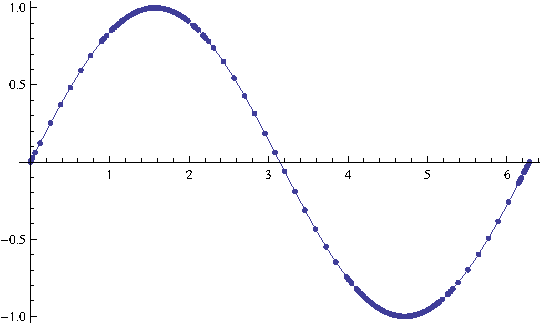
\includegraphics{figures/figmathematica_sinx}
\captionsetup{type=figure}%
			\caption{A graph of $y=\sin x$ generated by \textit{Mathematica}.}\label{fig:mathematica_sinx}
\end{minipage}\\
\vskip\baselineskip

How does \textit{Mathematica} know where the graph is ``curvy''? Calculus. When we study \textit{curvature} in a later chapter, we will see how the first and second derivatives of a function work together to provide a measurement of ``curviness.'' \textit{Mathematica} employs algorithms to determine regions of ``high curvature'' and plots extra points there.

Again, the goal of this section is not ``How to graph a function when there is no computer to help.'' Rather, the goal is ``Understand that the shape of the graph of a function is largely determined by understanding the behavior of the function at a few key places.'' In Example \ref{ex_sketch3}, we were able to accurately sketch a complicated graph using only 5 points and knowledge of asymptotes!

There are many applications of our understanding of derivatives beyond curve sketching. The next chapter explores some of these applications, demonstrating just a few kinds of problems that can be solved with a basic knowledge of differentiation. 

\printexercises{exercises/03_05_exercises}
%%
%%%%%\addtocounter{chapter}{3}
%
%\clearpage{\pagestyle{empty}\cleardoublepage}
%\chapter{Applications of the Derivative}\label{chapter:deriv_apps}
%\thispagestyle{empty}
%
%In Chapter \ref{chapter:graphbehavior}, we learned how the first and second derivatives of a function influence its graph. In this chapter we explore other applications of the derivative.


\section{Newton's Method}\label{sec:newton}
Solving equations is one of the most important things we do in mathematics, yet we are surprisingly limited in what we can solve analytically.  For instance, equations as simple as $x^5+x+1=0$ or $\cos x =x $ cannot be solved by algebraic methods in terms of familiar functions.  Fortunately, there are methods that can give us \textit{approximate} solutions to equations like these.  These methods can usually give an approximation correct to as many decimal places as we like. In Section \ref{sec:continuity} we learned about the Bisection Method.  This section focuses on another technique (which generally works faster), called Newton's Method.

%\vspace{.1in}\textbf{Newton's Method}\vspace{.1in}

Newton's Method is built around tangent lines.  The main idea is that if $x$ is sufficiently close to a root of $f(x)$, then the  tangent line to the graph at $(x,f(x))$ will cross the $x$-axis at a point closer to the root than $x$.  


\ifthenelse{\boolean{longpage}}% if longpage, draw in a row
{\noindent\begin{minipage}{.45\textwidth}\centering
\myincludegraphics{figures/fignewt1a} \\ (a)
\end{minipage}\hskip .1\textwidth
\begin{minipage}{.45\textwidth}\centering
\myincludegraphics{figures/fignewt1b} \\ (b)
\end{minipage}

\noindent\begin{minipage}{\textwidth}\centering
\myincludegraphics{figures/fignewt1c} \\ (c)
\captionsetup{type=figure}%
\caption{Demonstrating the geometric concept behind Newton's Method.}\label{fig:newt1}
\end{minipage}
}
{\mtable{.5}{Demonstrating the geometric concept behind Newton's Method.}{fig:newt1}{\begin{tabular}{c}\myincludegraphics{figures/fignewt1a}\\(a)\\\myincludegraphics{figures/fignewt1b} \\ (b) \\ \myincludegraphics{figures/fignewt1c} \\ (c) \end{tabular}
}
}

We start Newton's Method with an initial guess about roughly where the root is.  Call this $x_0$. (See Figure \ref{fig:newt1}(a).)  Draw the tangent line to the graph at $(x_0,f(x_0))$ and see where it meets the $x$-axis. Call this point $x_1$.  Then repeat the process -- draw the tangent line to the graph at $(x_1, f(x_1))$ and see where it meets the $x$-axis. (See Figure \ref{fig:newt1}(b).) Call this point $x_2$.  Repeat the process again to get $x_3$, $x_4$, etc.  This sequence of points will often converge rather quickly to a root of $f$.  

We can use this \textit{geometric} process to create an \textit{algebraic} process.  Let's look at how we found $x_1$.  We started with the tangent line to the graph at $(x_0,f(x_0))$.  The slope of this tangent line is $\fp(x_0)$ and the equation of the line is
$$y=\fp(x_0)(x-x_0)+f(x_0).$$
This line crosses the $x$-axis when $y=0$, and the $x$--value where it crosses is what we called $x_1$. So let $y=0$ and replace $x$ with $x_1$, giving the equation: 
$$ 0 = \fp(x_0)(x_1-x_0)+f(x_0).$$ 
Now solve for $x_1$:
$$x_1=x_0-\frac{f(x_0)}{\fp(x_0)}.$$
Since we repeat the same geometric process to find $x_2$ from $x_1$, we have
$$x_2=x_1-\frac{f(x_1)}{\fp(x_1)}.$$
In general, given an approximation $x_n$, we can find the next approximation, $x_{n+1}$ as follows:
$$x_{n+1} = x_{n} - \frac{f(x_{n})}{\fp(x_{n})}.$$

We summarize this process as follows.

\keyidea{idea:Newton}{Newton's Method}
{Let $f$ be a differentiable function on an interval $I$ with a root in $I$. To approximate the value of the root, accurate to $d$ decimal places:\index{Newton's Method}
	\begin{enumerate}
	\item		Choose a value $x_0$ as an initial approximation of the root. (This is often done by looking at a graph of $f$.)
	\item		Create successive approximations iteratively; given an approximation $x_n$, compute the next approximation $x_{n+1}$ as $$x_{n+1} = x_n - \frac{f(x_n)}{\fp(x_n)}.$$
	\item		Stop the iterations when successive approximations do not differ in the first $d$ places after the decimal point.
		\end{enumerate}
}

\mnote{.5}{\textbf{Note:} Newton's Method is not infallible. The sequence of approximate values may not converge, or it may converge so slowly that one is ``tricked'' into thinking a certain approximation is better than it actually is. These issues will be discussed at the end of the section.}

Let's practice Newton's Method with a concrete example.\\

\example{ex_newt2}{Using Newton's Method}{
Approximate the real root of $x^3-x^2-1=0$,  accurate to the first 3 places after the decimal, using Newton's Method and an initial approximation of $x_0=1$.}
{To begin, we compute $\fp(x)=3x^2-2x$.  Then we apply the Newton's Method algorithm, outlined in Key Idea \ref{idea:Newton}. 
\begin{align*}
x_1&=1-\frac{f(1)}{\fp(1)}=1-\frac{1^3-1^2-1}{3\cdot 1^2-2\cdot 1}=2,\\
x_2&=2-\frac{f(2)}{\fp(2)}=2-\frac{2^3-2^2-1}{3\cdot 2^2-2\cdot 2}=1.625,\\
x_3&=1.625-\frac{f(1.625)}{\fp(1.625)} = 1.625-\frac{1.625^3-1.625^2-1}{3\cdot 1.625^2-2\cdot 1.625}\approx 1.48579. \\
x_4 &= 1.48579 - \frac{f(1.48579)}{\fp(1.48579)} \approx  1.46596\\
x_5 &= 1.46596 - \frac{f(1.46596)}{\fp(1.46596)} \approx 1.46557
\end{align*}
We performed 5 iterations of Newton's Method to find a root accurate to the first 3 places after the decimal; our final approximation is $1.465.$ The exact value of the root, to six decimal places, is $1.465571$;  It turns out that our $x_5$ is accurate to more than just 3 decimal places.

A graph of $f(x)$ is given in Figure \ref{fig:newt2}. We can see from the graph that our initial approximation of $x_0=1$ was not particularly accurate; a closer guess would have been $x_0=1.5$. Our choice was based on ease of initial calculation, and shows that Newton's Method can be robust enough that we do not have to make a very accurate initial approximation.
\mfigure{.7}{A graph of $f(x) = x^3-x^2-1$ in Example \ref{ex_newt2}.}{fig:newt2}{figures/fignewt2}
}\\   

We can automate this process on a calculator that has an \verb+Ans+ key that returns the result of the previous calculation.  Start by pressing \verb+1+ and then \texttt{Enter}. (We have just entered our initial guess, $x_0=1$.)  Now  compute $$\text{\tt Ans} - \frac{f(\text{\tt Ans})}{\fp(\text{\tt Ans})}$$ by entering the following and repeatedly press the \texttt{Enter} key:
\begin{center}
\verb+Ans-(Ans^3-Ans^2-1)/(3*Ans^2-2*Ans)+
\end{center}
Each time we press the \texttt{Enter} key, we are finding the successive approximations, $x_1$, $x_2$, \dots, and each one is getting closer to the root.  In fact, once we get past around $x_7$ or so, the approximations don't appear to be changing.  They actually are changing, but the change is far enough to the right of the decimal point that it doesn't show up on the calculator's display.  When this happens, we can be pretty confident that we have found an accurate approximation.

Using a calculator in this manner makes the calculations simple; many iterations can be computed very quickly. \\

%In general, one would usually run Newton's Method in this way, finding approximations until the difference between two successive approximations is less than some prescribed tolerance, like maybe $10^{-10}$, whatever is necessary for the problem at hand.

\example{ex_newt3}{Using Newton's Method to find where functions intersect}{
Use Newton's Method to approximate a solution to $\cos{x} = x$, accurate to 5 places after the decimal.}
{Newton's Method provides a method of solving $f(x) = 0$; it is not (directly) a method for solving equations like $f(x) = g(x)$. However, this is not a problem; we can rewrite the latter equation as $f(x) - g(x)=0$ and then use Newton's Method. 

So we rewrite $\cos x=x$ as $\cos{x}-x=0$.  Written this way, we are finding a root of $f(x)=\cos{x}-x$.  We compute $\fp(x)=-\sin{x} - 1$.  Next we need a starting value, $x_0$.  Consider Figure \ref{fig:newt3}, where $f(x) = \cos x-x$ is graphed. It seems that $x_0=0.75$ is pretty close to the root, so we will use that as our $x_0$. (The figure also shows the graphs of $y=\cos x$ and $y=x$, drawn with dashed lines. Note how they intersect at the same $x$ value as when $f(x) = 0$.)

\mfigure{.7}{A graph of $f(x)=\cos x-x$ used to find an initial approximation of its root.}{fig:newt3}{figures/fignewt3}

We now compute $x_1$, $x_2$, etc.  The formula for $x_1$ is 
$$x_1 = 0.75 - \frac{\cos(0.75)-0.75}{-\sin(0.75)-1}\approx 0.7391111388.$$
%To 11 decimal places, this gives .7391111388.  We then compute 
Apply Newton's Method again to find $x_2$:
$$x_2 = 0.7391111388 - \frac{\cos(0.7391111388)-0.7391111388}{-\sin(0.7391111388)-1}\approx 0.7390851334.$$
We can continue this way, but it is really best to automate this process.  On a calculator with an Ans key, we would start by pressing 0.75, then \texttt{Enter}, inputting our initial approximation. We then enter:
%\begin{verbatim}
\begin{center}\texttt{Ans - (cos(Ans)-Ans)/(-sin(Ans)-1)}.\end{center}
%\end{verbatim}

Repeatedly pressing the \texttt{Enter} key gives successive approximations.  We quickly find:
\begin{align*}
x_3 &= 0.7390851332\\
x_4 &= 0.7390851332.
\end{align*}
Our approximations $x_2$ and $x_3$ did not differ for at least the first 5 places after the decimal, so we could have stopped. However, using our calculator in the manner described is easy, so finding $x_4$ was not hard. It is interesting to see how we found an approximation, accurate to as many decimal places as our calculator displays, in just 4 iterations.
}\\

If you know how to program, you can translate the following pseudocode into your favorite language to perform the computation in this problem.
\begin{center}
\begin{verbatim}
x = .75
while true
    oldx = x
    x = x - (cos(x)-x)/(-sin(x)-1)
    print x
    if abs(x-oldx) < .0000000001
        break
\end{verbatim}
\end{center}

This code calculates $x_1$, $x_2$, etc., storing each result in the variable \texttt{x}.  The previous approximation is stored in the variable \texttt{oldx}.  We continue looping until the difference between two successive approximations, \texttt{abs(x-oldx)}, is less than some small tolerance, in this case,
\texttt{.0000000001}.\\

\noindent\textbf{\large Convergence of Newton's Method}
\vskip \baselineskip

What should one use for the initial guess, $x_0$?  Generally, the closer to the actual root the initial guess is, the better.  However, some initial guesses should be avoided.  For instance, consider Example \ref{ex_newt2} where we sought the root to $f(x) = x^3-x^2-1$.  Choosing  $x_0=0$ would have been a particularly poor choice. Consider Figure \ref{fig:newt2a}, where $f(x)$ is graphed along with its tangent line at $x=0$. Since $\fp(0)=0$, the tangent line is horizontal and does not intersect the $x$--axis. Graphically, we see that Newton's Method fails.

\mfigure{.8}{A graph of $f(x) = x^3-x^2-1$, showing why an initial approximation of $x_0=0$ with Newton's Method fails.}{fig:newt2a}{figures/fignewt2a}

We can also see analytically that it fails. Since $$x_1 = 0 -\frac{f(0)}{\fp(0)}$$ and $\fp(0)=0$, we see that $x_1$ is not well defined.  

This problem can also occur if, for instance, it turns out that $\fp(x_5)=0$. Adjusting the initial approximation $x_0$ by a very small amount will likely fix the problem.

It is also possible for Newton's Method to not converge while each successive approximation is well defined. Consider $f(x) = x^{1/3}$, as shown in Figure \ref{fig:newt4}. It is clear that the root is $x=0$, but let's approximate this with $x_0=0.1$. Figure \ref{fig:newt4}(a) shows graphically the calculation of $x_1$; notice how it is farther from the root than $x_0$. Figures \ref{fig:newt4}(b) and (c) show the calculation of $x_2$ and $x_3$, which are even farther away; our successive approximations are getting worse. (It turns out that in this particular example, each successive approximation is twice as far from the true answer as the previous approximation.)

\ifthenelse{\boolean{longpage}}% if longpage, draw in a row
{\noindent\begin{minipage}{.45\textwidth}\centering
\myincludegraphics{figures/fignewt4a} \\ (a)
\end{minipage}\hskip .1\textwidth
\begin{minipage}{.45\textwidth}\centering
\myincludegraphics{figures/fignewt4b} \\ (b)
\end{minipage}

\noindent\begin{minipage}{\textwidth}\centering
\myincludegraphics{figures/fignewt4c} \\ (c)
\captionsetup{type=figure}%
\caption{Newton's Method fails to find a root of $f(x) = x^{1/3}$, regardless of the choice of $x_0$.}\label{fig:newt4}
\end{minipage}
}% not long page
{\mtable{.4}{Newton's Method fails to find a root of $f(x) = x^{1/3}$, regardless of the choice of $x_0$.}{fig:newt4}{\begin{tabular}{c}\myincludegraphics{figures/fignewt4a}\\(a)\\\myincludegraphics{figures/fignewt4b} \\ (b) \\ \myincludegraphics{figures/fignewt4c} \\ (c) \end{tabular}
}
}

There is no ``fix'' to this problem; Newton's Method simply will not work and another method must be used.


%There are other things that can go wrong with Newton's Method.  For instance, $f(x)=\sqrt[3]{x}$ has a vertical tangent line near its root at $x=0$.  This has the effect of actually pushing the approximations away from the root.  

While Newton's Method does not always work, it does work ``most of the time,'' and it is generally very fast. Once the approximations get close to the root, Newton's Method can as much as double the number of correct decimal places with each successive approximation. A course in Numerical Analysis will introduce the reader to more iterative root finding methods, as well as give greater detail about the strengths and weaknesses of Newton's Method.

%Despite the fact that Newton's Method won't always work, it does work quite often. And it is quick.  A lot of the time, once the approximations get close to the root, Newton's Method can as much as double the number of correct decimal places with each successive approximation.  Newton's Method and other methods that are related to it are what calculators and computer algebras systems use to find approximate solutions to equations.

\printexercises{exercises/04_01_exercises}
%\section{Related Rates}\label{sec:related_rates}

When two quantities are related by an equation, knowing the value of one quantity can determine the value of the other. For instance, the circumference and radius of a circle are related by $C=2\pi r$; knowing that $C = 6\pi$in determines the radius must be 3in.

The topic of \sword{related rates} takes this one step further: knowing the \textit{rate} at which one quantity is changing can determine the \textit{rate} at which the other changes.\index{related rates}\\

\mnote{.5}{\textbf{Note:} This section relies heavily on implicit differentiation, so referring back to Section \ref{sec:imp_deriv} may help.}

We demonstrate the concepts of related rates through examples.\\

\example{ex_rr1}{Understanding related rates}{
The radius of a circle is growing at a rate of 5in/hr. At what rate is the circumference growing?}
{The circumference and radius of a circle are related by $C = 2\pi r$. We are given information about how the length of $r$ changes with respect to time; that is, we are told $\frac{dr}{dt} = 5$in/hr. We want to know how the length of $C$ changes with respect to time, i.e., we want to know $\frac{dC}{dt}$. 

Implicitly differentiate both sides of $C = 2\pi r$ with respect to $t$:
\begin{align*}
C 	&= 2\pi r\\
\frac{d}{dt}\big(C\big) &= \frac{d}{dt}\big(2\pi r\big) \\
\frac{dC}{dt} 	&=	2\pi \frac{dr}{dt}.
\end{align*}
As we know $\frac{dr}{dt} = 5$in/hr, we know $$\frac{dC}{dt} = 2\pi 5 = 10\pi \approx 31.4\text{in/hr.}$$
\vskip-\baselineskip}\\

Consider another, similar example.\\

\example{ex_rr2}{Finding related rates}{
Water streams out of a faucet at a rate of $2$in$^3$/s onto a flat surface at a constant rate, forming a circular puddle that is $1/8$in deep. 
\begin{enumerate}
\item		At what rate is the area of the puddle growing?
\item		At what rate is the radius of the circle growing?
\end{enumerate}
}
{\begin{enumerate}
\item We can answer this question two ways: using ``common sense'' or related rates. The common sense method states that the volume of the puddle is growing by $2$in$^3$/s, where 
	\begin{center} volume of puddle $=$ area of circle $\times$ depth.\end{center}
Since the depth is constant at $1/8$in, the area must be growing by 16in$^2$/s.

This approach reveals the underlying related--rates principle. Let $V$ and $A$ represent the Volume and Area of the puddle. We know $V= A\times \frac18$. Take the derivative of both sides with respect to $t$, employing implicit differentiation.
\begin{align*}
V &= \frac18A\\
\frac{d}{dt}\big(V\big) &= \frac{d}{dt}\left(\frac18A\right)\\
\frac{dV}{dt} &=	\frac18\frac{dA}{dt}
\end{align*} 
As $\frac{dV}{dt} = 2$, we know $2 = \frac18\frac{dA}{dt}$, and hence $\frac{dA}{dt} = 16$. Thus the area is growing by 16in$^2$/s.

\drawexampleline
\item		To start, we need an equation that relates what we know to the radius. We just learned something about the surface area of the circular puddle, and we know $A = \pi r^2$. We should be able to learn about the rate at which the radius is growing with this information. 

Implicitly derive both sides of $A=\pi r^2$ with respect to $t$:
\begin{align*}
	A 	&= \pi r^2 \\
	\frac{d}{dt}\big(A\big) &= \frac{d}{dt}\big(\pi r^2\big)\\
	\frac{dA}{dt} &= 2\pi r\frac{dr}{dt}
\end{align*}

Our work above told us that $\frac{dA}{dt} = 16$in$^2$/s. Solving for $\frac{dr}{dt}$, we have $$\frac{dr}{dt} = \frac{8}{\pi r}.$$

Note how our answer is not a number, but rather a function of $r$. In other words, \textit{the rate at which the radius is growing depends on how big the circle already is.} If the circle is very large, adding 2in$^3$ of water will not make the circle much bigger at all. If the circle is dime--sized, adding the same amount of water will make a radical change in the radius of the circle.

In some ways, our problem was (intentionally) ill--posed. We need to specify a current radius in order to know a rate of change. When the puddle has a radius of 10in, the radius is growing at a rate of $$
\frac{dr}{dt} = \frac{8}{10\pi} = \frac{4}{5\pi} \approx 0.25\text{in/s}.$$
 
\end{enumerate}
\vskip-2\baselineskip
}\\

\example{ex_rr3}{Studying related rates}{
Radar guns measure the rate of distance change between the gun and the object it is measuring. For instance, a reading of ``55mph'' means the object is moving away from the gun at a rate of 55 miles per hour, whereas a measurement of ``$-25$mph'' would mean that the object is approaching the gun at a rate of 25 miles per hour.

If the radar gun is moving (say, attached to a police car) then radar readouts are only immediately understandable if the gun and the object are moving along the same line. If a police officer is traveling 60mph and gets a readout of 15mph, he knows that the car ahead of him is moving away at a rate of 15 miles an hour, meaning the car is traveling 75mph. (This straight--line principle is one reason officers park on the side of the highway and try to shoot straight back down the road. It gives the most accurate reading.)

Suppose an officer is driving due north at 30 mph and sees a car moving due east, as shown in Figure \ref{fig:rr3}. Using his radar gun, he measures a reading of 20mph. By using landmarks, he believes both he and the other car are about 1/2 mile from the intersection of their two roads. 

\mfigure{.35}{A sketch of a police car (at bottom) attempting to measure the speed of a car (at right) in Example \ref{ex_rr3}.}{fig:rr3}{figures/figrr3}

If the speed limit on the other road is 55mph, is the other driver speeding?}
{Using the diagram in Figure \ref{fig:rr3}, let's label what we know about the situation. As both the police officer and other driver are 1/2 mile from the intersection, we have $A = 1/2$, $B = 1/2$, and through the Pythagorean Theorem, $C = 1/\sqrt{2}\approx 0.707$. 

We know the police officer is traveling at 30mph; that is, $\frac{dA}{dt} = -30$. The reason this rate of change is negative is that $A$ is getting smaller; the distance between the officer and the intersection is shrinking. The radar measurement is $\frac{dC}{dt} = 20$. We want to find $\frac{dB}{dt}$. 

We need an equation that relates $B$ to $A$ and/or $C$. The Pythagorean Theorem is a good choice: $A^2+B^2 = C^2$. Differentiate both sides with respect to $t$:
\begin{align*}
		A^2 + B^2 &= C^2 \\
		\frac{d}{dt}\left(A^2+B^2\right) &= \frac{d}{dt}\left(C^2\right) \\
		2A\frac{dA}{dt} + 2B\frac{dB}{dt} &= 2C\frac{dC}{dt}
\end{align*}

We have values for everything except $\frac{dB}{dt}$. Solving for this we have 
		$$\frac{dB}{dt} = \frac{C\frac{dC}{dt}- A\frac{dA}{dt}}{B} \approx 58.28\text{mph}.$$
		
The other driver appears to be speeding slightly.		
}\\

\mnote{.8}{\textbf{Note:} Example \ref{ex_rr3} is both interesting and impractical. It highlights the difficulty in using radar in a non--linear fashion, and explains why ``in real life'' the police officer would follow the other driver to determine their speed, and not pull out pencil and paper.

The principles here are important, though. Many automated vehicles make judgments about other moving objects based on perceived distances, radar--like measurements and the concepts of related rates.}

\example{ex_rr4}{Studying related rates}{
A camera is placed on a tripod 10ft from the side of a road. The camera is to turn to track a car that is to drive by at 100mph for a promotional video. The video's planners want to know what kind of motor the tripod should be equipped with in order to properly track the car as it passes by.  Figure \ref{fig:rr4} shows the proposed setup.

\mfigure{.5}{Tracking a speeding car (at left) with a rotating camera.}{fig:rr4}{figures/figrr4}

How fast must the camera be able to turn to track the car?
}
{We seek information about how fast the camera is to \textit{turn}; therefore, we need an equation that will relate an angle $\theta$ to the position of the camera and the speed and position of the car.

Figure \ref{fig:rr4} suggests we use a trigonometric equation. Letting $x$ represent the distance the car is from the point on the road directly in front of the camera, we have \begin{equation}\tan \theta = \frac{x}{10}.\label{eq:rr4}\end{equation} As the car is moving at 100mph, we have $\frac{dx}{dt} = -100$mph (as in the last example, since $x$ is getting smaller as the car travels, $\frac{dx}{dt}$ is negative). We need to convert the measurements so they use the same units; rewrite -100mph in terms of ft/s:
$$\frac{dx}{dt} = -100\frac{\text{m}}{\text{hr}} = -100\frac{\text{m}}{\text{hr}}\cdot5280\frac{\text{ft}}{\text{m}}\cdot\frac{1}{3600}\frac{\text{hr}}{\text{s}} =-146.\overline{6}\text{ft/s}.$$
Now take the derivative of both sides of Equation \eqref{eq:rr4} using implicit differentiation:
\begin{align}
		\tan \theta &= \frac{x}{10} \notag \\
		\frac{d}{dt}\big(\tan \theta\big) &= \frac{d}{dt}\left(\frac{x}{10}\right)\notag \\
		\sec^2\theta\,\frac{d\theta}{dt} &= \frac{1}{10}\frac{dx}{dt}\notag\\
		\frac{d\theta}{dt} &= \frac{\cos^2\theta}{10}\frac{dx}{dt}\label{eq:rr4b}
\end{align}
We want to know the fastest the camera has to turn. Common sense tells us this is when the car is directly in front of the camera (i.e., when $\theta = 0$). Our mathematics bears this out. In Equation \eqref{eq:rr4b} we see this is when $\cos^2\theta$ is largest; this is when $\cos \theta = 1$, or when $\theta = 0$.

With $\frac{dx}{dt} \approx -146.67$ft/s, we have 
	$$\frac{d\theta}{dt} = -\frac{1\text{rad}}{10\text{ft}}146.67\text{ft/s} = -14.667\text{radians/s}.$$
We find that $\frac{d\theta}{dt}$ is negative; this matches our diagram in Figure \ref{fig:rr4} for $\theta$ is getting smaller as the car approaches the camera.	
	
What is the practical meaning of $-14.667$radians/s? Recall that 1 circular revolution goes through $2\pi$ radians, thus $14.667$rad/s means $14.667/(2\pi)\approx 2.33$ revolutions per second. The negative sign indicates the camera is rotating in a clockwise fashion.
}\\

We introduced the derivative as a function that gives the slopes of tangent lines of functions. This chapter emphasizes using the derivative in other ways. Newton's Method uses the derivative to approximate roots of functions; this section stresses the ``rate of change'' aspect of the derivative to find a relationship between the rates of change of two related quantities. 

In the next section we use Extreme Value concepts to \textit{optimize} quantities. 

\printexercises{exercises/04_02_exercises}
%\section{Optimization}\label{sec:optimization}

In Section \ref{sec:extreme_values} we learned about extreme values -- the largest and smallest values a function attains on an interval. We motivated our interest in such values by discussing how it made sense to want to know the highest/lowest values of a stock, or the fastest/slowest an object was moving. In this section we apply the concepts of extreme values to solve ``word problems,'' i.e., problems stated in terms of situations that require us to create the appropriate mathematical framework in which to solve the problem.\index{optimization}

\enlargethispage{\baselineskip}
We start with a classic example which is followed by a discussion of the topic of optimization.\\

\example{ex_opt1}{Optimization: perimeter and area}{
A man has 100 feet of fencing, a large yard, and a small dog. He wants to create a rectangular enclosure for his dog with the fencing that provides the maximal area. What dimensions provide the maximal area?}
{One can likely guess the correct answer -- that is great. We will proceed to show how calculus can provide this answer in a context that proves this answer is correct.

It helps to make a sketch of the situation. Our enclosure is sketched twice in Figure \ref{fig:opt1}, either with green grass and nice fence boards or as a simple rectangle. Either way, drawing a rectangle forces us to realize that we need to know the dimensions of this rectangle so we can create an area function -- after all, we are trying to maximize the area.

\ifthenelse{\boolean{longpage}}% longpage
{\noindent\begin{center}
\myincludegraphics{figures/figopt1b}
\captionsetup{type=figure}%
\caption{A sketch of the enclosure in Example \ref{ex_opt1}.}\label{fig:opt1}
\end{center}
} % end longpage
{\mfigure{.5}{A sketch of the enclosure in Example \ref{ex_opt1}.}{fig:opt1}{figures/figopt1a}
} %end regular page


We let $x$ and $y$ denote the lengths of the sides of the rectangle. Clearly, $$\text{Area}=xy.$$

We do not yet know how to handle functions with 2 variables; we need to reduce this down to a single variable. We know more about the situation: the man has 100 feet of fencing. By knowing the perimeter of the rectangle must be 100, we can create another equation: $$\text{Perimeter} = 100 = 2x+2y.$$

We now have 2 equations and 2 unknowns. In the latter equation, we solve for $y$:
$$y = 50-x.$$ Now substitute this expression for $y$ in the area equation:
$$ \text{Area} = A(x) = x(50-x).$$ Note we now have an equation of one variable; we can truly call the Area a function of $x$. 

This function only makes sense when $0\leq x \leq 50$, otherwise we get negative values of area. So we find the extreme values of $A(x)$ on the interval $[0,50]$. 

To find the critical points, we take the derivative of $A(x)$ and set it equal to 0, then solve for $x$.
\begin{align*}
A(x) &= x(50-x) \\
			&= 50x-x^2 \\
A'(x) 	&= 50-2x
\end{align*}
We solve $50-2x=0$ to find $x=25$; this is the only critical point. We evaluate $A(x)$ at the endpoints of our interval and at this critical point to find the extreme values; in this case, all we care about is the maximum.

Clearly $A(0)=0$ and $A(50)=0$, whereas $A(25) = 625 \text{ft}^2$. This is the maximum. Since we earlier found $y = 50-x$, we find that $y$ is also $25$. Thus the dimensions of the rectangular enclosure with perimeter of 100 ft. with maximum area is a square, with sides of length 25 ft.
}\\

This example is very simplistic and a bit contrived. (After all, most people create a design then buy fencing to meet their needs, and not buy fencing and plan later.) But it models well the necessary process: create equations that describe a situation, reduce an equation to a single variable, then find the needed extreme value.

``In real life,'' problems are much more complex. The equations are often \textit{not} reducible to a single variable (hence multi--variable calculus is needed) and the equations themselves may be difficult to form. Understanding the principles here will provide a good foundation for the mathematics you will likely encounter later.

We outline here the basic process of solving these optimization problems.
\enlargethispage{2\baselineskip}
%\small
\keyidea{idea:optimization}{Solving Optimization Problems}
{\begin{enumerate}
		\item		Understand the problem. Clearly identify what quantity is to be maximized or minimized. Make a sketch if helpful.
		\item		Create equations relevant to the context of the problem, using the information given. (One of these should describe the quantity to be optimized. We'll call this the \textit{fundamental equation.})
		\item		If the fundamental equation defines the quantity to be optimized as a function of more than one variable, reduce it to a single variable function using substitutions derived from the other equations.
		\end{enumerate}
\textit{\small (continued)$\ldots$}
}

\addtocounter{keyideacounter}{-1}
\keyidea{idea:optimizationb}{Solving Optimization Problems -- Continued}
{\begin{enumerate}\addtocounter{enumi}{3}
		\item		Identify the domain of this function, keeping in mind the context of the problem.
		\item		Find the extreme values of this function on the determined domain.
		\item		Identify the values of all relevant quantities of the problem.
		\end{enumerate}
}
%\normalsize

We will use Key Idea \ref{idea:optimization} in a variety of examples.\\

\example{ex_opt2}{Optimization: perimeter and area}{
Here is another classic calculus problem: A woman has a 100 feet of fencing, a small dog, and a large yard that contains a stream (that is mostly straight). She wants to create a rectangular enclosure with maximal area that uses the stream as one side. (Apparently her dog won't swim away.) What dimensions provide the maximal area?}
{We will follow the steps outlined by Key Idea \ref{idea:optimization}. 
	\begin{enumerate}
	\item		We are maximizing \textit{area}. A sketch of the region will help; Figure \ref{fig:opt2} gives two sketches of the proposed enclosed area. A key feature of the sketches is to acknowledge that one side is not fenced. 
	
\mfigure{.4}{A sketch of the enclosure in Example \ref{ex_opt2}.}{fig:opt2}{figures/figopt2a}
	
	\item		We want to maximize the area; as in the example before, $$\text{Area} = xy.$$ This is our fundamental equation. This defines area as a function of two variables, so we need another equation to  reduce it to one variable. 
	
	We again appeal to the perimeter; here the perimeter is $$\text{Perimeter} = 100 = x+2y.$$ Note how this is different than in our previous example.
	\item		We now reduce the fundamental equation to a single variable. In the perimeter equation, solve for $y$: $y = 50 - x/2$. We can now write Area as $$\text{Area} = A(x) = x(50-x/2) = 50x - \frac12x^2.$$ Area is now defined as a function of one variable.
	\item		We want the area to be nonnegative. Since $A(x) = x(50-x/2)$, we want $x\geq 0$ and $50-x/2\geq 0$. The latter inequality implies that $x\leq100$, so $0\leq x\leq 100$. 
	\item		We now find the extreme values. At the endpoints, the minimum is found, giving an area of 0. 
	
	Find the critical points. We have $A'(x) = 50-x$; setting this equal to 0 and solving for $x$ returns $x=50$. This gives an area of $$A(50) = 50(25) = 1250.$$
	\item		We earlier set $y = 50-x/2$; thus $y = 25$. Thus our rectangle will have two sides of length 25 and one side of length 50, with a total area of 1250 ft$^2$.
	\end{enumerate}
\vskip-\baselineskip
}\\

Keep in mind as we do these problems that we are practicing a \textit{process}; that is, we are learning to turn a situation into a system of equations. These equations allow us to write a certain quantity as a function of one variable, which we then optimize.\\

%\mnote{.5}{\textbf{Note:} Example \ref{ex_opt3} is another classic calculus example. The underlying principle is given in a variety of contexts; Google ``calculus dog'' to find articles where 

\example{ex_opt3}{Optimization: minimizing cost}{
A power line needs to be run from an power station located on the beach to an offshore facility. Figure \ref{fig:opt3b} shows the distances between the power station to the facility.

It costs \$50/ft. to run a power line along the land, and \$130/ft. to run a power line under water. How much of the power line should be run along the land to minimize the overall cost? What is the minimal cost?

\mfigure{.5}{Running a power line from the power station to an offshore facility with minimal cost in Example \ref{ex_opt3}.}{fig:opt3b}{figures/figopt3b}
}
{We will follow the strategy of Key Idea \ref{idea:optimization} implicitly, without specifically numbering steps.

There are two immediate solutions that we could consider, each of which we will reject through ``common sense.'' First, we could minimize the distance by directly connecting the two locations with a straight line. However, this requires that all the wire be laid underwater, the most costly option. Second, we could minimize the underwater length by running a wire all 5000 ft. along the beach, directly across from the offshore facility. This has the undesired effect of having the longest distance of all, probably ensuring a non--minimal cost.

The optimal solution likely has the line being run along the ground for a while, then underwater, as the figure implies. We need to label our unknown distances -- the distance run along the ground and the distance run underwater. Recognizing that the underwater distance can be measured as the hypotenuse of a right triangle, we choose to label the distances as shown in Figure \ref{fig:opt3c}.

\mfigure{.3}{Labeling unknown distances in Example \ref{ex_opt3}.}{fig:opt3c}{figures/figopt3c}

By choosing $x$ as we did, we make the expression under the square root simple. We now create the cost function. 

$$
\begin{array}{ccccc}
\text{Cost} &=&  \text{land cost} &+ & \text{water cost} \\
						&	& \text{\$50}\times \text{land distance} &+& \text{\$130}\times \text{water distance} \\
						&	& 50(5000-x) &+& 130\sqrt{x^2+1000^2}.\\
\end{array}
$$

So we have $c(x) = 50(5000-x)+ 130\sqrt{x^2+1000^2}$. This function only makes sense on the interval $[0,5000]$. While we are fairly certain the endpoints will not give a minimal cost, we still evaluate $c(x)$ at each to verify.
$$c(0) = 380,000 \quad\quad c(5000) \approx 662,873.$$

We now find the critical values of $c(x)$. We compute $c\primeskip'(x)$ as 
$$c\primeskip'(x) = -50+\frac{130x}{\sqrt{x^2+1000^2}}.$$

Recognize that this is never undefined. Setting $c\primeskip'(x)=0$ and solving for $x$, we have:
\begin{align*}
-50+\frac{130x}{\sqrt{x^2+1000^2}} &= 0 \\
\frac{130x}{\sqrt{x^2+1000^2}}  &= 50\\
\frac{130^2x^2}{x^2+1000^2} &= 50^2\\
130^2x^2 &= 50^2(x^2+1000^2) \\
130^2x^2-50^2x^2 &= 50^2\cdot1000^2\\
(130^2-50^2)x^2 &= 50,000^2\\
x^2 &= \frac{50,000^2}{130^2-50^2}\\
x &= \frac{50,000}{\sqrt{130^2-50^2}}\\
x & = \frac{50,000}{120} =416\frac23\approx 416.67.
\end{align*}

Evaluating $c(x)$ at $x=416.67$ gives a cost of about \$370,000. The distance the power line is laid along land is $5000-416.67 = 4583.33$ ft., and the underwater distance is $\sqrt{416.67^2+1000^2} \approx 1083$ ft.
%\mnote{.5}{\textbf{Note:} This minimal cost is \$10,000 less than the cost of simply minimizing the underwater distance, a savings of about 3\%. Is t
}\\

In the exercises you will see a variety of situations that require you to combine problem--solving skills with calculus. Focus on the \textit{process}; learn how to form equations from situations that can be manipulated into what you need. Eschew memorizing how to do ``this kind of problem'' as opposed to ``that kind of problem.'' Learning a process will benefit one far longer than memorizing a specific technique.

The next section introduces our final application of the derivative: \textit{differentials}. Given $y=f(x)$, they offer a method of approximating the change in $y$ after $x$ changes by a small amount. 

\printexercises{exercises/04_03_exercises}
		
%\section{Differentials}\label{sec:differentials}

In Section \ref{sec:interp_deriv} we explored the meaning and use of the derivative. This section starts by revisiting some of those ideas.

Recall that the derivative of a function $f$ can be used to find the slopes of lines tangent to the graph of $f$. At $x=c$, the tangent line to the graph of $f$ has equation $$y = \fp(c)(x-c)+f(c).$$
The tangent line can be used to find good approximations of $f(x)$ for values of $x$ near $c$. 

For instance, we can approximate $\sin 1.1$ using the tangent line to the graph of $f(x)=\sin x$ at $x=\pi/3 \approx 1.05.$ Recall that $\sin (\pi/3) = \sqrt{3}/2 \approx 0.866$, and $\cos (\pi/3) = 1/2$. Thus the tangent line to $f(x) = \sin x$ at $x=\pi/3$ is: $$ \ell(x) = \frac12(x-\pi/3)+0.866.$$



\ifthenelse{\boolean{longpage}}% if longpage, draw in a row
{\noindent%
\begin{minipage}{\textwidth}\centering
\noindent\begin{minipage}{.45\textwidth}\centering
\noindent\myincludegraphics{figures/figdiffal1a} \\ (a)
\end{minipage}\hskip .05\textwidth
\begin{minipage}{.45\textwidth}\centering
\noindent\myincludegraphics{figures/figdiffal1} \\ (b)
\end{minipage}
\captionsetup{type=figure}%
\caption{Graphing $f(x) = \sin x$ and its tangent line at $x=\pi/3$ in order to estimate $\sin 1.1$.}\label{fig:diffal1}
\end{minipage}
}
{\mtable{.5}{Graphing $f(x) = \sin x$ and its tangent line at $x=\pi/3$ in order to estimate $\sin 1.1$.}{fig:diffal1}{\begin{tabular}{c}
\myincludegraphics{figures/figdiffal1a}\\[10pt]
(a)\\[10pt]
\myincludegraphics{figures/figdiffal1} \\[10pt]
 (b)\end{tabular}
}
}

In Figure \ref{fig:diffal1}(a), we see a graph of $f(x) = \sin x$ graphed along with its tangent line at $x=\pi/3$. The small rectangle shows the region that is displayed in Figure \ref{fig:diffal1}(b). In this figure, we see how we are approximating $\sin 1.1$ with the tangent line, evaluated at $1.1$. Together, the two figures show how close these values are.

Using this line to approximate $\sin 1.1$, we have:
\begin{align*}
	\ell(1.1) &= \frac12(1.1-\pi/3)+0.866 \\
					&= \frac12(0.053)+0.866 = 0.8925.
\end{align*}
(We leave it to the reader to see how good of an approximation this is.)\\

We now generalize this concept. Given $f(x)$ and an $x$--value $c$,  the tangent line is $\ell(x) = \fp(c)(x-c)+f(c)$. Clearly, $f(c) = \ell(c)$. Let $\dx$ be a small number, representing a small change in $x$ value. We assert that:
$$f(c+\dx) \approx \ell(c+\dx),$$ since the tangent line to a function approximates well the values of that function near $x=c$. 

As the $x$-value changes from $c$ to $c+\dx$, the $y$-value of $f$ changes from $f(c)$ to $f(c+\dx)$. We call this change of $y$ value \dy. That is:
$$\dy = f(c+\dx)-f(c).$$
Replacing $f(c+\dx)$ with its tangent line approximation, we have 
\begin{align} \dy &\approx \ell(c+\dx) - f(c) \notag\\
								&= \fp(c)\big((c+\dx)-c\big)+f(c) - f(c)\notag \\
								&=\fp(c)\dx		\label{eq:differential}
\end{align}

This final equation is important; it becomes the basis of the upcoming Definition and Key Idea. In short, it says that when the $x$-value changes from $c$ to $c+\Delta x$, the $y$ value of a function $f$ changes by about $\fp(c)\Delta x$.

We introduce two new variables, $dx$ and $dy$ in the context of a formal definition. %We defined $dx = \dx$; that is, it is a small change in $x$. We define

\definition{def:differential}{Differentials of $x$ and $y$.}
{Let $y=f(x)$ be differentiable. The \textbf{differential of $x$}, denoted $dx$, is any nonzero real number (usually taken to be a small number).\index{differential}\index{derivative!differential} The \textbf{differential of $y$}, denoted $dy$, is $$dy = \fp(x)dx.$$
}

We can solve for $\fp(x)$ in the above equation: $\fp(x) = dy/dx$. This states that the derivative of $f$ with respect to $x$ is the differential of $y$ divided by the differential of $x$; this is \textbf{not} the alternate notation for the derivative, $\frac{dy}{dx}$. This latter notation was chosen because of the fraction--like qualities of the derivative, but again, it is one symbol and not a fraction.

It is helpful to organize our new concepts and notations in one place.

\keyidea{idea:differential}{Differential Notation}
{Let $y = f(x)$ be a differentiable function. \index{differential!notation}
\begin{enumerate}
	\item Let $\dx$ represent a small, nonzero change in $x$ value.
	\item	Let $dx$ represent a small, nonzero change in $x$ value (i.e., $\dx = dx$).
	\item	Let $\dy$ be the change in $y$ value as $x$ changes by $\dx$; hence $$\dy = f(x+\dx)-f(x).$$
	\item		Let $dy = \fp(x)dx$ which, by Equation (\ref{eq:differential}), is an \textit{approximation} of the change in $y$ value as $x$ changes by $\dx$; $dy \approx \dy$.
\end{enumerate}
}

What is the value of differentials? Like many mathematical concepts, differentials provide both practical and theoretical benefits. We explore both here.\\

\example{ex_diffal1}{Finding and using differentials}{
Consider $f(x) = x^2$. Knowing $f(3) = 9$, approximate $f(3.1)$.}
{The $x$ value is changing from $x=3$ to $x=3.1$; therefore, we see that $dx=0.1$. If we know how much the $y$ value changes from $f(3)$ to $f(3.1)$ (i.e., if we know $\dy$), we will know exactly what $f(3.1)$ is (since we already know $f(3)$). We can approximate \dy\ with $dy$.
\begin{align*} \dy &\approx dy \\
								  &= \fp(3)dx \\
								  &= 2\cdot 3\cdot 0.1 = 0.6.
\end{align*}

We expect the $y$ value to change by about $0.6$, so we approximate $f(3.1) \approx 9.6.$

We leave it to the reader to verify this, but the preceding discussion links the differential to the tangent line of $f(x)$ at $x=3$. One can verify that the tangent line, evaluated at $x=3.1$, also gives $y=9.6$.
}\\

Of course, it is easy to compute the actual answer (by hand or with a calculator): $3.1^2 = 9.61.$ (Before we get too cynical and say ``Then why bother?'', note our approximation is \textit{really} good!)

So why bother?

In ``most'' real life situations, we do not know the function that describes a particular behavior. Instead, we can only take measurements of how things change -- measurements of the derivative.

Imagine water flowing down a winding channel. It is easy to measure the speed and direction (i.e., the \textit{velocity}) of water at any location. It is very hard to create a function that describes the overall flow, hence it is hard to predict where a floating object placed at the beginning of the channel will end up. However, we can \textit{approximate} the path of an object using differentials. Over small intervals, the path taken by a floating object is essentially linear. Differentials allow us to approximate the true path by piecing together lots of short, linear paths. This technique is called Euler's Method, studied in introductory Differential Equations courses.

We use differentials once more to approximate the value of a function. Even though calculators are very accessible, it is neat to see how these techniques can sometimes be used to easily compute something that looks rather hard.\\

%\enlargethispage{\baselineskip}

\example{ex_diffal2}{Using differentials to approximate a function value}{
Approximate $\sqrt{4.5}$.}
{We expect $\sqrt{4.5} \approx 2$, yet we can do better. Let $f(x) = \sqrt{x}$, and let $c=4$. Thus $f(4) = 2$. We can compute $\fp(x) = 1/(2\sqrt{x})$, so $\fp(4) = 1/4$. 

We approximate the difference between $f(4.5)$ and $f(4)$ using differentials, with $dx = 0.5$:
$$f(4.5)-f(4) = \dy \approx dy = \fp(4)\cdot dx = 1/4 \cdot 1/2 = 1/8 = 0.125.$$
The approximate change in $f$ from $x=4$ to $x=4.5$ is $0.125$, so we approximate $\sqrt{4.5} \approx 2.125.$
}\\

Differentials are important when we discuss \textit{integration}. When we study that topic, we will use notation such as $$\int f(x)\ dx$$ quite often. While we don't discuss here what all of that notation means, note the existence of the differential $dx$. Proper handling of \textit{integrals} comes with proper handling of differentials. 

In light of that, we practice finding differentials in general.\\

\example{ex_diffal3}{Finding differentials}{
In each of the following, find the differential $dy$.

\begin{center}
1. $y = \sin x$ \qquad\quad 2. $y = e^x(x^2+2)$ \quad\qquad 3. $y = \sqrt{x^2+3x-1}$
\end{center}
}
{\begin{enumerate}
\item		$y = \sin x$:	\quad As $f(x) = \sin x$, $\fp(x) = \cos x$. Thus $$dy = \cos (x)dx.$$

\item		$y = e^x(x^2+2)$:\quad Let $f(x) = e^x(x^2+2)$. We need $\fp(x)$, requiring the Product Rule. 

We have $\fp(x) = e^x(x^2+2) + 2xe^x$, so $$dy = \big(e^x(x^2+2) + 2xe^x\big)dx.$$

\item		$y = \sqrt{x^2+3x-1}$:\quad	Let $f(x) = \sqrt{x^2+3x-1}$; we need $\fp(x)$, requiring the Chain Rule.

We have $\ds \fp(x) = \frac{1}{2}(x^2+3x-1)^{-\frac12}(2x+3) = \frac{2x+3}{2\sqrt{x^2+3x-1}}.$ Thus 
$$ dy = \frac{(2x+3)dx}{2\sqrt{x^2+3x-1}}.$$
\end{enumerate}
\vskip-\baselineskip
}\\
%\clearpage

Finding the differential $dy$ of $y=f(x)$ is really no harder than finding the derivative of $f$; we just \textit{multiply} $\fp(x)$ by $dx$. It is important to remember that we are not simply adding the symbol ``$dx$'' at the end.\\

We have seen a practical use of differentials as they offer a good method of making certain approximations. Another use is \textit{error propagation.} Suppose a length is measured to be $x$, although the actual value is $x+\dx$ (where \dx\ is the error, which we hope  is small). This measurement of $x$ may be used to compute some other value; we can think of this latter value as $f(x)$ for some function $f$. As the true length is $x+\dx$, one really should have computed $f(x+\dx)$. The difference between $f(x)$ and $f(x+\dx)$ is the propagated error. 

How close are $f(x)$ and $f(x+\dx)$? This is a difference in ``y'' values: $$f(x+\dx)-f(x) = \dy \approx dy.$$ We can approximate the propagated error using differentials.\\

\example{ex_diffal4}{Using differentials to approximate propagated error}{
A steel ball bearing is to be manufactured with a diameter of 2cm. The manufacturing process has a tolerance of $\pm 0.1$mm in the diameter. Given that the density of steel is about 7.85g/cm$^3$, estimate the propagated error in the mass of the ball bearing.}
{The mass of a ball bearing is found using the equation ``mass = volume $\times$ density.'' In this situation the mass function is a product of the radius of the ball bearing, hence it is $m = 7.85\frac43\pi r^3$. The differential of the mass is $$dm = 31.4\pi r^2 dr.$$ The radius is to be 1cm; the manufacturing tolerance in the radius is $\pm 0.05$mm, or $\pm 0.005$cm. The propagated error is approximately:
\begin{align*}
\Delta m & \approx dm \\
				&= 31.4\pi (1)^2 (\pm 0.005) \\
				&= \pm 0.493\text{g}
\end{align*}
Is this error significant? It certainly depends on the application, but we can get an idea by computing the \textit{relative error}. The ratio between amount of error to the total mass is
\begin{align*}
\frac{dm}{m} &= \pm \frac{0.493}{7.85\frac43\pi} \\
							&=\pm \frac{0.493}{32.88}\\
							&=\pm 0.015,
\end{align*}
or $\pm 1.5$\%. 

\enlargethispage{\baselineskip}

We leave it to the reader to confirm this, but if the diameter of the ball was supposed to be 10cm, the same manufacturing tolerance would give a propagated error in mass of $\pm12.33$g, which corresponds to a \textit{percent error} of $\pm0.188$\%. While the amount of error is much greater ($12.33 > 0.493$), the percent error is much lower.
}\\

We first learned of the derivative in the context of instantaneous rates of change and slopes of tangent lines. We furthered our understanding of the power of the derivative by studying how it relates to the graph of a function (leading to ideas of increasing/decreasing and concavity). This chapter has put the derivative to yet more uses:
\begin{itemize}
\item Equation solving (Newton's Method),
\item	Related Rates (furthering our use of the derivative to find instantaneous rates of change),
\item	Optimization (applied extreme values), and
\item	Differentials (useful for various approximations and for something called integration).
\end{itemize}

In the next chapters, we will consider the ``reverse'' problem to computing the derivative: given a function $f$, can we find a function whose derivative is $f$\hskip.75pt? Being able to do so opens up an incredible world of mathematics and applications.

%\refstepcounter{definitioncounter}
%\label{lastdefcount1}
%\refstepcounter{theoremcounter}
%\label{lastthmcount1}
%\refstepcounter{keyideacounter}
%\label{lastideacount1}
%\addtocounter{definitioncounter}{-1}
%\addtocounter{theoremcounter}{-1}
%\addtocounter{keyideacounter}{-1}
%\refstepcounter{examplecounter}
%\label{lastexamplecount1}
%\addtocounter{examplecounter}{-1}

\printexercises{exercises/04_04_exercises}
%%
%%
%%
%\refstepcounter{definitioncounter}
%\label{lastdefcount1}
%\refstepcounter{theoremcounter}
%\label{lastthmcount1}
%\refstepcounter{keyideacounter}
%\label{lastideacount1}
%\refstepcounter{examplecounter}
%\label{lastexamplecount1}
%\addtocounter{definitioncounter}{-1}
%\addtocounter{theoremcounter}{-1}
%\addtocounter{keyideacounter}{-1}
%\addtocounter{examplecounter}{-1}
%%
%%
%%%%
%%%%%\addtocounter{chapter}{4}
%%
%\clearpage{\pagestyle{empty}\cleardoublepage}
%\chapter{Integration}\label{chapter:integration}
%\thispagestyle{empty}
%\addtocontents{toc}{\protect\thispagestyle{empty}}

%We have spent considerable time considering the derivatives of a function and their applications. In the following chapters, we are going to starting thinking in ``the other direction.'' That is, given a function $f(x)$, we are going to consider functions $F(x)$ such that $F\primeskip'(x) = f(x)$. There are numerous reasons this will prove to be useful: these functions will help us compute area, volume, mass, force, pressure, work, and much more.



\section{Antiderivatives and Indefinite Integration}\label{sec:antider}

Given a function $y=f(x)$, a \textit{differential equation} is one that incorporates $y$, $x$, and the derivatives of $y$. For instance, a simple differential equation is: $$y\primeskip' = 2x.$$

Solving a differential equation amounts to finding a function $y$ that satisfies the given equation. Take a moment and consider that equation; can you find a function $y$ such that $y\primeskip' = 2x$?

Can you find another?

And yet another?

Hopefully one was able to come up with at least one solution: $y = x^2$. ``Finding another'' may have seemed impossible until one realizes that a function like $y=x^2+1$ also has a derivative of $2x$. Once that discovery is made, finding ``yet another'' is not difficult; the function $y = x^2 + 123,456,789$ also has a derivative of $2x$. The differential equation $y\primeskip' = 2x$ has many solutions. This leads us to some definitions.
%\enlargethispage{3\baselineskip}

\definition{def:antider}{Antiderivatives and Indefinite Integrals}
{Let a function $f(x)$ be given. An \textbf{antiderivative} of $f(x)$ is a function $F(x)$ such that $\Fp(x) = f(x)$.\index{antiderivative}\index{indefinite integral}\index{integration!indefinite}\\

The set of all antiderivatives of $f(x)$ is the \textbf{indefinite integral of $f$}, denoted by $$\int f(x) \ dx.$$
}

Make a note about our definition: we refer to \textit{an} antiderivative of $f$, as opposed to \textit{the} antiderivative of $f$, since there is \textit{always} an infinite number of them. We often use upper-case letters to denote antiderivatives.

Knowing one antiderivative of $f$ allows us to find infinitely more, simply by adding a constant. Not only does this give us \textit{more} antiderivatives, it gives us \textit{all} of them.

\theorem{thm:antideriv_const}{Antiderivative Forms}
{Let $F(x)$ and $G(x)$ be antiderivatives of $f(x)$ on an interval $I$. Then there exists a constant $C$ such that, on $I$,  $$G(x) = F(x) + C.$$
}

Given a function $f$ defined on an interval $I$ and one of its antiderivatives $F$, we know \textit{all} antiderivatives of $f$ on $I$ have the form $F(x) + C$ for some constant $C$. Using Definition \ref{def:antider}, we can say that $$\int f(x) \ dx = F(x) + C.$$

Let's analyze this indefinite integral notation.\index{integration!notation}

\begin{center}
\myincludegraphics{figures/figanti1}
\captionsetup{type=figure}%
\caption{Understanding the indefinite integral notation.}\label{fig:anti1}
\end{center}

Figure \ref{fig:anti1} shows the typical notation of the indefinite integral. The integration symbol, $\int$, is in reality an ``elongated S,'' representing ``take the sum.'' We will later see how \textit{sums} and \textit{antiderivatives} are related.

The function we want to find an antiderivative of is called the \textit{integrand}. It contains the differential of the variable we are integrating with respect to. The $\int$ symbol and the differential $dx$ are not ``bookends'' with a function sandwiched in between; rather, the symbol $\int$ means ``find all antiderivatives of what follows,'' and the function $f(x)$ and $dx$ are multiplied together; the $dx$ does not ``just sit there.''

Let's practice using this notation.\\

\example{ex_anti2}{Evaluating indefinite integrals}{
Evaluate $\displaystyle \int \sin x\ dx.$}
{We are asked to find all functions $F(x)$ such that $\Fp(x) = \sin x$. Some thought will lead us to one solution: $F(x) = -\cos x$, because $\frac{d}{dx}(-\cos x) = \sin x$.

The indefinite integral of $\sin x$ is thus $-\cos x$, plus a constant of integration. So:
$$\int \sin x \ dx = -\cos x + C.$$
\vskip-\baselineskip
}\\

A commonly asked question is ``What happened to the $dx$?'' The unenlightened response is ``Don't worry about it. It just goes away.'' A full understanding includes the following.

This process of \textit{antidifferentiation} is really solving a \textit{differential} question. The integral $$\int \sin x\ dx$$ presents us with a differential, $dy = \sin x\ dx$. It is asking: ``What is $y$?'' We found lots of solutions, all of the form $y = -\cos x+C$.

%We can view integration in the following way. 
Letting $dy = \sin x\ dx$,  rewrite 
$$\int \sin x \ dx \quad \text{as}\quad \int  dy.$$
This is asking: ``What functions have a differential of the form $dy$?'' The answer is ``Functions of the form $y+C$, where $C$ is a constant.'' What is $y$? We have lots of choices, all differing by a constant; the simplest choice is $y = -\cos x$.

Understanding all of this is more important later as we try to find antiderivatives of more complicated functions. In this section, we will simply explore the rules of indefinite integration, and one can succeed for now with answering ``What happened to the $dx$?'' with ``It went away.''

Let's practice once more before stating integration rules.\\

\example{ex_anti3}{Evaluating indefinite integrals}{
Evaluate $\ds \int (3x^2 + 4x+5)\ dx$.}
{We seek a function $F(x)$ whose derivative is $3x^2+4x+5$. When taking derivatives, we can consider functions term--by--term, so we can likely do that here.

What functions have a derivative of $3x^2$? Some thought will lead us to a cubic, specifically $x^3+C_1$, where $C_1$ is a constant. 

What functions have a derivative of $4x$? Here the $x$ term is raised to the first power, so we likely seek a quadratic. Some thought should lead us to $2x^2+C_2$, where $C_2$ is a constant.

Finally, what functions have a derivative of $5$? Functions of the form $5x+C_3$, where $C_3$ is a constant.

Our answer appears to be 
$$\int (3x^2+4x+5)\ dx = x^3+C_1+2x^2+C_2+5x+C_3.$$ We do not need three separate constants of integration; combine them as one constant, giving the final answer of 
$$\int (3x^2+4x+5)\ dx = x^3+2x^2+5x+C.$$

It is easy to verify our answer; take the derivative of $x^3+2x^3+5x+C$ and see we indeed get $3x^2+4x+5$.
}\\

This final step of ``verifying our answer'' is important both practically and theoretically. In general, taking derivatives is easier than finding antiderivatives so checking our work is easy and vital as we learn.

We also see that taking the derivative of our answer returns the function in the integrand. Thus we can say that: $$\frac{d}{dx}\left(\int f(x)\ dx\right) = f(x).$$
Differentiation ``undoes'' the work done by antidifferentiation. 

Theorem \ref{thm:deriv_glossary} gave a list of the derivatives of common functions we had learned at that point. We restate part of that list here to stress the relationship between derivatives and antiderivatives. This list will also be useful as a glossary of common antiderivatives as we learn.

\newlength{\bh}%box height
\newlength{\bd}%box depth
\settoheight{\bh}{$\frac{d}{dx}$}
\settodepth{\bd}{$\frac{d}{dx}$}

%\newcommand{\myrule}{\rule[-\bd]{0pt}{\bh+\bd}}%\ $\frac{d}{dx}$
%\newcommand{\myrule}{\rule[-4pt]{0pt}{13pt}}%\ $\frac{d}{dx}$

\theorem{thm:indef_alg}{Derivatives and Antiderivatives}
{\begin{minipage}[t]{.45\specialboxlength}
Common Differentiation Rules\rule[-2pt]{0pt}{1pt}
\begin{enumerate}
\item \myrule$\frac{d}{dx}\big(cf(x) \big) = c\cdot \fp(x)$
\item \myrule$\frac{d}{dx}\big(f(x)\pm g(x) \big) = $
\vskip .05\baselineskip
\myrule$\fp(x)\pm g'(x)$
\item $\frac{d}{dx}\big(C \big) = 0$\myrule
\item $\frac{d}{dx}\big(x \big) = 1$\myrule
\item $\frac{d}{dx}\big(x^n \big) = n\cdot x^{n-1}$\myrule
\item $\frac{d}{dx}\big(\sin x \big) = \cos x$\myrule
\item $\frac{d}{dx}\big(\cos x \big) = -\sin x$\myrule
\item $\frac{d}{dx}\big(\tan x \big) = \sec^2 x$\myrule
\item $\frac{d}{dx}\big(\csc x \big) = -\csc x\cot x$\myrule
\item $\frac{d}{dx}\big(\sec x \big) = \sec x\tan x$\myrule
\item $\frac{d}{dx}\big(\cot x \big) = -\csc^2 x$\myrule
\item $\frac{d}{dx}\big(e^ x \big) = e^x$\myrule
\item $\frac{d}{dx}\big(a^x \big) = \ln a\cdot a^x$\myrule
\item $\frac{d}{dx}\big(\ln x \big) = \frac1 x$\myrule
\end{enumerate}
\end{minipage}
\begin{minipage}[t]{.55\specialboxlength}
Common Indefinite Integral Rules\rule[-2pt]{0pt}{1pt}
\begin{enumerate}
\item \myrule$\int c\cdot f(x)\ dx = c\cdot \int f(x)\ dx$
\item \myrule$\int \big(f(x)\pm g(x)\big)\ dx =$
\vskip .05\baselineskip
\myrule$ \int f(x)\ dx\pm \int g(x)\ dx$
\item $\int 0\ dx = C$\myrule
\item $\int 1\ dx = \int dx = x+C$\myrule
\item $\int x^n\ dx =\frac{1}{n+1}x^{n+1}+ C$\quad {\scriptsize ($n\neq -1$)}\myrule
\item $\int \cos x\ dx = \sin x+C$\myrule
\item $\int \sin x\ dx = -\cos x+C$\myrule
\item $\int \sec^2 x\ dx = \tan x+C$\myrule
\item $\int \csc x\cot  x\ dx = -\csc x+C$\myrule
\item $\int \sec x\tan x\ dx = \sec x+C$\myrule
\item $\int \csc^2 x\ dx = -\cot x+C$\myrule
\item $\int e^x\ dx = e^x+C$\myrule
\item $\int a^x\ dx = \frac{1}{\ln a}\cdot a^x+C$\myrule
\item $\int \frac{1}x\ dx = \ln |x|+C$\myrule
\end{enumerate}
\end{minipage}%\\
%
%\textit{\small (continued $\ldots$)}
}
%\addtocounter{theoremcounter}{-1}
%
%\theorem{thm:indef_algb}{Derivatives and Antiderivatives -- Continued}
%{\begin{minipage}[t]{.45\specialboxlength}
%Common Differentiation Rules\rule[-2pt]{0pt}{1pt}
%\begin{enumerate}\addtocounter{enumi}{5}
%%\item \myrule$\frac{d}{dx}\big(cf(x) \big) = c\cdot \fp(x)$
%%\item \myrule$\frac{d}{dx}\big(f(x)\pm g(x) \big) = $
%%\vskip .05\baselineskip
%%\myrule$\fp(x)\pm g'(x)$
%%\item $\frac{d}{dx}\big(C \big) = 0$\myrule
%%\item $\frac{d}{dx}\big(x \big) = 1$\myrule
%%\item $\frac{d}{dx}\big(x^n \big) = n\cdot x^{n-1}$\myrule
%\item $\frac{d}{dx}\big(\sin x \big) = \cos x$\myrule
%\item $\frac{d}{dx}\big(\cos x \big) = -\sin x$\myrule
%\item $\frac{d}{dx}\big(\tan x \big) = \sec^2 x$\myrule
%\item $\frac{d}{dx}\big(\csc x \big) = -\csc x\cot x$\myrule
%\item $\frac{d}{dx}\big(\sec x \big) = \sec x\tan x$\myrule
%\item $\frac{d}{dx}\big(\cot x \big) = -\csc^2 x$\myrule
%\item $\frac{d}{dx}\big(e^ x \big) = e^x$\myrule
%\item $\frac{d}{dx}\big(a^x \big) = \ln a\cdot a^x$\myrule
%\item $\frac{d}{dx}\big(\ln x \big) = \frac1 x$\myrule
%\end{enumerate}
%\end{minipage}
%\begin{minipage}[t]{.55\specialboxlength}
%Common Indefinite Integral Rules\rule[-2pt]{0pt}{1pt}
%\begin{enumerate}\addtocounter{enumi}{5}
%%\item \myrule$\int c\cdot f(x)\ dx = c\cdot \int f(x)\ dx$
%%\item \myrule$\int \big(f(x)\pm g(x)\big)\ dx =$
%%\vskip .05\baselineskip
%%\myrule$ \int f(x)\ dx\pm \int g(x)\ dx$
%%\item $\int 0\ dx = C$\myrule
%%\item $\int 1\ dx = \int dx = x+C$\myrule
%%\item $\int x^n\ dx =\frac{1}{n+1}x^{n+1}+ C$\quad {\scriptsize ($n\neq -1$)}\myrule
%\item $\int \cos x\ dx = \sin x+C$\myrule
%\item $\int \sin x\ dx = -\cos x+C$\myrule
%\item $\int \sec^2 x\ dx = \tan x+C$\myrule
%\item $\int \csc x\cot  x\ dx = -\csc x+C$\myrule
%\item $\int \sec x\tan x\ dx = \sec x+C$\myrule
%\item $\int \csc^2 x\ dx = -\cot x+C$\myrule
%\item $\int e^x\ dx = e^x+C$\myrule
%\item $\int a^x\ dx = \frac{1}{\ln a}\cdot a^x+C$\myrule
%\item $\int \frac{1}x\ dx = \ln |x|+C$\myrule
%\end{enumerate}
%\end{minipage}
%}

We highlight a few important points from Theorem \ref{thm:indef_alg}:
\begin{itemize}
	\item		Rule \#1 states $\int c\cdot f(x)\ dx = c\cdot \int f(x)\ dx$. This is the Constant Multiple Rule: \index{Constant Multiple Rule!of integration} we can temporarily ignore constants when finding antiderivatives, just as we did when computing derivatives (i.e., $\frac{d}{dx}\big(3x^2\big)$ is just as easy to compute as $\frac{d}{dx}\big(x^2\big)$). An example:
	$$\int 5\cos x\ dx = 5\cdot\int \cos x\ dx = 5\cdot (\sin x+C) = 5\sin x + C.$$
	In the last step we can consider the constant as also being multiplied by 5, but ``5 times a constant'' is still a constant, so we just write ``$C$\,''.
	\item		Rule \#2 is the Sum/Difference Rule:\index{integration!Sum/Difference Rule}\index{Sum/Difference Rule!of integration} we can split integrals apart when the integrand contains terms that are added/subtracted, as we did in Example \ref{ex_anti3}. So:
	\begin{align*}
	\int(3x^2+4x+5)\ dx &= \int 3x^2\ dx + \int 4x\ dx + \int 5\ dx \\
											&= 3\int x^2\ dx + 4\int x\ dx + \int 5 \ dx\\
											&= 3\cdot \frac13x^3 + 4\cdot \frac12x^2+5x+C\\
											&= x^3+2x^2+5x+C
	\end{align*}
	In practice we generally do not write out all these steps, but we demonstrate them here for completeness.
	\item		Rule \#5 is the Power Rule of indefinite integration.\index{integration!Power Rule}\index{Power Rule!integration} There are two important things to keep in mind:
		\begin{enumerate}
		\item		Notice the restriction that $n\neq -1$. This is important: $\int \frac{1}{x}\ dx \neq $ ``$\frac{1}{0}x^0+C$''; rather, see Rule \#14.
		\item		We are presenting antidifferentiation as the ``inverse operation'' of differentiation. Here is a useful quote to remember:
		\begin{quote}%\centering
		``Inverse operations do the opposite things in the opposite order.''
		\end{quote}
		When taking a derivative using the Power Rule, we \textbf{first} \textit{multiply} by the power, then \textbf{second} \textit{subtract} 1 from the power. To find the antiderivative, do the opposite things in the opposite order: \textbf{first} \textit{add} one to the power, then \textbf{second} \textit{divide} by the power.
			\end{enumerate}
		\item		Note that Rule \#14 incorporates the absolute value of $x$. The exercises will work the reader through why this is the case; for now, know the absolute value is important and cannot be ignored.
\end{itemize}

\enlargethispage{\baselineskip}
\vskip\baselineskip
\noindent\textbf{\large Initial Value Problems}
\vskip\baselineskip

In Section \ref{sec:basic_diff_rules} we saw that the derivative of a position function gave a velocity function, and the derivative of a velocity function describes  acceleration.\index{initial value problem} We can now go ``the other way:'' the antiderivative of an acceleration function gives a velocity function, etc. While there is just one derivative of a given function, there are infinitely many antiderivatives. Therefore we cannot ask ``What is \textit{the} velocity of an object whose acceleration is $-32$ft/s$^2$?'', since there is more than one answer. 

We can find \textit{the} answer if we provide more information with the question, as done in the following example. Often the additional information comes in the form of an \textit{initial value}, a value of the function that one knows beforehand.\\

\example{ex_anti4}{Solving initial value problems}{
The acceleration due to gravity of a falling object is $-32$ ft/s$^2$. At time $t=3$, a falling object had a velocity of $-10$ ft/s. Find the equation of the object's velocity.}
{We want to know a velocity function, $v(t)$. We know two things:
	\begin{itemize}
		\item		The acceleration, i.e., $v\primeskip'(t)= -32$, and
		\item		the velocity at a specific time, i.e., $v(3) = -10$.
	\end{itemize}
Using the first piece of information, we know that $v(t)$ is an antiderivative of $v\primeskip'(t)=-32$. So we begin by finding the indefinite integral of $-32$:
		$$\int (-32)\ dt = -32t+C=v(t).$$
Now we use the fact that $v(3)=-10$ to find $C$:
\begin{align*}
	v(t) &= -32t+C \\
	v(3) &= -10 \\
	-32(3)+C &= -10\\
	C &= 86
\end{align*}

Thus $v(t)= -32t+86$. We can use this equation to understand the motion of the object: when $t=0$, the object had a velocity of $v(0) = 86$ ft/s. Since the velocity is positive, the object was moving upward.

When did the object begin moving down? Immediately after $v(t) = 0$:
$$-32t+86 = 0 \quad \Rightarrow\quad  t = \frac{43}{16}  \approx 2.69\text{s}.$$
Recognize that we are able to determine quite a bit about the path of the object knowing just its acceleration and its velocity at a single point in time.
}\\

\example{ex_anti5}{Solving initial value problems}{
Find $f(t)$, given that $\fpp(t) = \cos t$, $\fp(0) = 3$ and $f(0) = 5$.}
{We start by finding $\fp(t)$, which is an antiderivative of $\fpp(t)$:
		$$\int \fpp(t)\ dt = \int \cos t\ dt = \sin t + C = \fp(t).$$
		
		So $\fp(t) = \sin t+C$ for the correct value of $C$. We are given that $\fp(0) = 3$, so:
		$$\fp(0) = 3 \quad \Rightarrow \quad \sin 0+C = 3 \quad \Rightarrow \quad C=3.$$
		Using the initial value, we have found $\fp(t) = \sin t+ 3.$
		
We now find $f(t)$ by integrating again.

%\enlargethispage{3\baselineskip}
$$f(t)=\int \fp(t) \ dt = \int (\sin t+3)\ dt = -\cos t + 3t + C.$$ 
We are given that $f(0) = 5$, so
\begin{align*}
-\cos 0 + 3(0) + C &= 5 \\
-1 + C &= 5\\
C &= 6
\end{align*}
 Thus $f(t) = -\cos t + 3t + 6$.
}\\

This section introduced antiderivatives and the indefinite integral. We found they are needed when finding a function given information about its derivative(s). For instance, we found a velocity function given an acceleration function.

In the next section, we will see how position and velocity are unexpectedly related by the areas of certain regions on a graph of the velocity function. Then, in Section \ref{sec:FTC}, we will see how areas and antiderivatives are closely tied together. This connection is incredibly important, as indicated by the name of the theorem that describes it: The Fundamental Theorem of Calculus.

\printexercises{exercises/05_01_exercises}
%\addtocontents{toc}{\protect\thispagestyle{empty}}
%\section{The Definite Integral}\label{sec:def_int}

We start with an easy problem. An object travels in a straight line at a constant velocity of 5 ft/s for 10 seconds. How far away from its starting point is the object?

We approach this problem with the familiar ``Distance $=$ Rate $\times$ Time'' equation. In this case, Distance = 5ft/s $\times$ 10s $=$ 50 feet.

It is interesting to note that this solution of 50 feet can be represented graphically. Consider Figure \ref{fig:defint1}, where the constant velocity of 5ft/s is graphed on the axes. Shading the area under the line from $t=0$ to $t=10$ gives a rectangle with an area of 50 square units; when one considers the units of the axes, we can say this area represents 50 ft.

\mfigure{.8}{The area under a constant velocity function corresponds to distance traveled.}{fig:defint1}{figures/figdefint1}

Now consider a slightly harder situation (and not particularly realistic): an object travels in a straight line with a constant velocity of 5ft/s for 10 seconds, then instantly reverses course at a rate of 2ft/s for 4 seconds. (Since the object is traveling in the opposite direction when reversing course, we say the velocity is a constant $-2$ft/s.) How far away from the starting point is the object -- what is its \textit{displacement}?

Here we use ``Distance $=$ Rate$_1$ $\times$ Time$_1$ + Rate$_2$ $\times$ Time$_2$,'' which is 
	$$\text{Distance } \ = 5\cdot10 + (-2)\cdot 4 = 42\text{ ft.}$$ 
Hence the object is 42 feet from its starting location.

We can again depict this situation graphically. In Figure \ref{fig:defint2} we have the velocities graphed as straight lines on $[0,10]$ and $[10,14]$, respectively. The displacement of the object is 
		\begin{center}``Area above the $t$--axis \quad $-$\quad Area below the $t$--axis,''
		\end{center}
which is easy to calculate as $50-8=42$ feet.

\mfigure{.55}{The total displacement is the area above the $t$--axis minus the area below the $t$--axis.}{fig:defint2}{figures/figdefint2}

Now consider a more difficult problem.\\

\example{ex_defint3}{Finding position using velocity}{
The velocity of an object moving straight up/down under the acceleration of gravity is given as $v(t) = -32t+48$, where time $t$ is given in seconds and velocity is in ft/s. When $t=0$, the object had a height of 0 ft.
		\begin{enumerate}
		\item		What was the initial velocity of the object?
		\item		What was the maximum height of the object?
		\item		What was the height of the object at time $t=2$?
		\end{enumerate}
		
}
{It is straightforward to find the initial velocity; at time $t=0$, $v(0) =-32\cdot 0+48 = 48 $ ft/s.

To answer questions about the height of the object, we need to find the object's position function $s(t)$. This is an initial value problem, which we studied in the previous section. We are told the initial height is 0, i.e., $s(0) = 0$. We know $s\primeskip'(t) = v(t) = -32t+48$. To find $s$, we find the indefinite integral of $v(t)$:
		$$\int v(t)\ dt = \int (-32t+48)\ dt = -16t^2+48t+C = s(t).$$
Since $s(0) = 0$, we conclude that $C=0$ and $s(t) = -16t^2+48t$.

To find the maximum height of the object, we need to find the maximum of $s$. Recalling our work finding extreme values, we find the critical points of $s$ by setting its derivative equal to 0 and solving for $t$:
		$$s\primeskip'(t) = -32t+48 = 0 \quad \Rightarrow \quad t=48/32 = 1.5\text{s}.$$
(Notice how we ended up just finding when the velocity was 0ft/s!) The first derivative test shows this is a maximum, so the maximum height of the object is found at $$s(1.5) = -16(1.5)^2+48(1.5)=36\text{ft}.$$
The height at time $t=2$ is now straightforward to compute: it is $s(2) = 32$ft.\\

While we have answered all three questions, let's look at them again graphically, using the concepts of area that we explored earlier.


Figure \ref{fig:defint3} shows a graph of $v(t)$ on axes from $t=0$ to $t=3$. It is again straightforward to find $v(0)$. How can we use the graph to find the maximum height of the object?

\mfigure{.5}{A graph of $v(t)=-32t+48$; the shaded areas help determine displacement.}{fig:defint3}{figures/figdefint3}

Recall how in our previous work that the displacement of the object (in this case, its height) was found as the area under the velocity curve, as shaded in the figure. Moreover, the area between the curve and the $t$--axis that is below the $t$--axis counted as ``negative'' area. That is, it represents the object coming back toward its starting position. So to find the maximum distance from the starting point -- the maximum height -- we find the area under the velocity line that is above the $t$--axis, i.e., from $t=0$ to $t=1.5$. This region is a triangle; its area is 
$$\text{Area } = \frac12\text{Base} \times \text{Height} =\frac12\times 1.5\text{s}\times 48\text{ft/s} = 36\text{ft},$$
which matches our previous calculation of the maximum height.

%\enlargethispage{3\baselineskip}
\drawexampleline
%Finally, we find the total \textit{signed} area under the velocity function from $t=0$ to $t=2$ to find the $s(2)$, the height at $t=2$, which is a displacement, the distance from the current position to the starting position. 
Finally, to find the height of the object at time $t=2$ we calculate the total signed area under the velocity function from $t=0$ to $t=2$. This signed area is equal to $s(2)$, the displacement (i.e., signed distance) from the starting position at $t=0$ to the position at time $t=2$. That is,
	\begin{center}
	Displacement = Area above the $t$--axis $-$ Area below $t$--axis.
	\end{center}
	The regions are triangles, and we find 
	$$\text{Displacement} = \frac12(1.5\text{s})(48\text{ft/s}) - \frac12(.5\text{s})(16\text{ft/s}) = 32\text{ft}.$$
This also matches our previous calculation of the height at $t=2$.

Notice how we answered each question in this example in two ways. Our first method was to manipulate equations using our understanding of antiderivatives and derivatives. Our second method was geometric: we answered questions looking at a graph and finding the areas of certain regions of this graph.
%\vskip-\baselineskip
}\\

The above example does not \textit{prove} a relationship between area under a velocity function and displacement, but it does imply a relationship exists. Section \ref{sec:FTC} will fully establish fact that the area under a velocity function is displacement.

Given a graph of a function $y=f(x)$, we will find that there is great use in computing the area between the curve $y=f(x)$ and the $x$-axis. Because of this, we need to define some terms.

\definition{def:def_int}{The Definite Integral, Total Signed Area}
{Let $y=f(x)$ be defined on a closed interval $[a,b]$. The \textbf{total signed area from $x=a$ to $x=b$ under $f$} is:\index{integration!definite}\index{definite integral}\index{signed area}\index{total signed area}\index{integration!notation}\index{integration!area}

\noindent\parbox{\specialboxlength}{\centering (area  under $f$ and above the $x$--axis on $[a,b]$) $-$ (area above $f$ and under the $x$--axis on $[a,b]$).}\\

The \textbf{definite integral of $f$ on $[a,b]$} is the total signed area of $f$ on $[a,b]$, denoted $$\int_a^b f(x)\ dx,$$
where $a$ and $b$ are the \textbf{bounds of integration.}
}

By our definition, the definite integral gives the ``signed area under $f$.'' We usually drop the word ``signed'' when talking about the definite integral, and simply say the definite integral gives ``the area under $f$\,'' or, more commonly, ``the area under the curve.''

The previous section introduced the indefinite integral, which related to antiderivatives. We have now defined the definite integral, which relates to areas under a function. The two are very much related, as we'll see when we learn the Fundamental Theorem of Calculus in Section \ref{sec:FTC}. Recall that earlier we said that the ``$\int$'' symbol was an ``elongated S'' that represented finding a ``sum.'' In the context of the definite integral, this notation makes a bit more sense, as we are adding up areas under the function $f$.

We practice using this notation.\\

\example{ex_defint4}{Evaluating definite integrals}{
Consider the function $f$ given in Figure \ref{fig:defint4}.

\mfigure{.8}{A graph of $f(x)$ in Example \ref{ex_defint4}.}{fig:defint4}{figures/figdefint4}
 Find:

\noindent\begin{minipage}[t]{.45\textwidth}
\begin{enumerate}
		\item		$\ds \int_0^3 f(x)\ dx$
		\item		$\ds \int_3^5 f(x)\ dx$
		\item		$\ds \int_0^5 f(x)\ dx$
\end{enumerate}
\end{minipage}\hskip .05\textwidth
\begin{minipage}[t]{.45\textwidth}
		\begin{enumerate}\addtocounter{enumi}{3}
		\item		$\ds \int_0^3 5f(x)\ dx$
		\item		$\ds \int_1^1 f(x) \ dx$
\end{enumerate}
\end{minipage}

}
{\begin{enumerate}
		\item		$ \int_0^3 f(x)\ dx$ is the area under $f$ on the interval $[0,3]$. This region is a triangle, so the area is $\int_0^3 f(x)\ dx=\frac12(3)(1) = 1.5$. 
		\item		$\int_3^5 f(x)\ dx$ represents the area of the triangle found under the $x$--axis on $[3,5]$. The area is $\frac12(2)(1) = 1$; since it is found \textit{under} the $x$--axis, this is ``negative area.'' Therefore $ \int_3^5 f(x)\ dx = -1$.
		\item		$ \int_0^5f(x)\ dx$ is the total signed area under $f$ on $[0,5]$. This is $1.5 + (-1) = 0.5$.
		\item		$ \int_0^35f(x)\ dx$ is the area under $5f$ on $[0,3]$. This is sketched in Figure \ref{fig:defint4a}. Again, the region is a triangle, with height 5 times that of the height of the original triangle. Thus the area is $ \int_0^35f(x)\ dx = 15/2 = 7.5.$
		
\mfigure{.5}{A graph of $5f$ in Example \ref{ex_defint4}. (Yes, it looks just like the graph of $f$ in Figure \ref{fig:defint4}, just with a different $y$-scale.)}{fig:defint4a}{figures/figdefint4a}		
		
		\item		$\int_1^1f(x)\ dx$ is the area under $f$ on the ``interval'' $[1,1]$. This describes a line segment, not a region; it has no width. Therefore the area is 0.
\end{enumerate}
\vskip-\baselineskip
}\\

This example illustrates some of the properties of the definite integral, given here.

\theorem{thm:defintprop}{Properties of the Definite Integral}
{Let $f$ and $g$ be defined on a closed interval $I$ that contains the values $a$, $b$ and $c$, and let $k$ be a constant. The following hold:\index{integration!definite!properties}\index{definite integral!properties}
		\begin{enumerate}
		\item		$\ds \int_a^a f(x)\ dx = 0$
		\item		$\ds \int_a^b f(x)\ dx + \int_b^c f(x)\ dx = \int_a^cf(x)\ dx$
		\item		$\ds \int_a^bf(x)\ dx = -\int_b^a f(x)\ dx$
		\item		$\ds \int_a^b\big(f(x)\pm g(x)\big)\ dx = \int_a^bf(x)\ dx \pm \int_a^bg(x)\ dx$
		\item		$\ds \int_a^bk\cdot f(x)\ dx = k\cdot\int_a^bf(x)\ dx$
		\end{enumerate}
}

We give a brief justification of Theorem \ref{thm:defintprop} here.
		\begin{enumerate}
		\item		As demonstrated in Example \ref{ex_defint4}, there is no ``area under the curve'' when the region has no width; hence this definite integral is 0.
		\item		This states that total area is the sum of the areas of subregions. It is easily considered when we let $a<b<c$. We can break the interval $[a,c]$ into two subintervals, $[a,b]$ and $[b,c]$. The total area over $[a,c]$ is the area over $[a,b]$ plus the area over $[b,c]$. 
		
		It is important to note that this still holds true even if $a<b<c$ is not true. We discuss this in the next point.
		\item		This property can be viewed a merely a convention to make other properties work well. (Later we will see how this property has a justification all its own, not necessarily in support of other properties.) Suppose $b<a<c$. The discussion from the previous point clearly justifies 
		\begin{equation}\int_b^a f(x)\ dx + \int_a^c f(x)\ dx = \int_b^c f(x)\ dx.\label{eq:defint1}\end{equation}
		However, we still claim that, as originally stated, 
		\begin{equation}\int_a^b f(x)\ dx + \int_b^c f(x)\ dx = \int_a^c f(x)\ dx.\label{eq:defint2}\end{equation}
		How do Equations (\ref{eq:defint1}) and (\ref{eq:defint2}) relate? Start with Equation (\ref{eq:defint1}):
		\begin{align*}
		\int_b^a f(x)\ dx + \int_a^c f(x)\ dx &= \int_b^c f(x)\ dx\\
		\int_a^c f(x)\ dx &= -\int_b^a f(x)\ dx + \int_b^c f(x)\ dx\\
		\end{align*}
Property $(3)$ justifies changing the sign and switching the bounds of integration on the $\ds -\int_b^a f(x)\ dx$ term; when this is done, Equations (\ref{eq:defint1}) and (\ref{eq:defint2}) are equivalent.

The conclusion is this: by adopting the convention of Property (3), Property (2) holds no matter the order of $a$, $b$ and $c$. Again, in the next section we will see another justification for this property.
	\item[4,5.]	Each of these may be non--intuitive. Property (5) states that when one scales a function by, for instance, 7, the area of the enclosed region also is scaled by a factor of 7. Both Properties (4) and (5)  can be proved using geometry. The details are not complicated but are not discussed here.
\end{enumerate}

%\enlargethispage{2\baselineskip}%\clearpage
\example{ex_defint5}{Evaluating definite integrals using Theorem \ref{thm:defintprop}.}
{Consider the graph of a function $f(x)$ shown in Figure \ref{fig:defint5}. 
\mfigure{.5}{A graph of a function in Example \ref{ex_defint5}.}{fig:defint5}{figures/figdefint5}
Answer the following:
		\begin{enumerate}
		\item		Which value is greater: $\ds \int_a^b f(x)\ dx$ or $\ds \int_b^c f(x)\ dx$?
		\item		Is $\ds \int_a^c f(x)\ dx$ greater or less than 0?
		\item		Which value is greater: $\ds \int_a^b f(x)\ dx$ or $\ds \int_c^b f(x)\ dx$?
		\end{enumerate}
		
}
{\begin{enumerate}
		\item		$\int_a^b f(x)\ dx$ has a positive value (since the area is above the $x$--axis) whereas $\int_b^c f(x)\ dx$ has a negative value. Hence $\int_a^b f(x)\ dx$ is bigger.
		\item		$\int_a^c f(x)\ dx$ is the total signed area under $f$ between $x=a$ and $x=c$. Since the region below the $x$--axis looks to be larger than the region above, we conclude that the definite integral has a value less than 0.
		\item		Note how the second integral has the bounds ``reversed.'' Therefore $\int_c^b f(x)\ dx$ represents a positive number, greater than the area described by the first definite integral. Hence $\int_c^b f(x)\ dx$ is greater.
		\end{enumerate}
\vskip-1.5\baselineskip
}\clearpage

The area definition of the definite integral allows us to use geometry compute the definite integral of some simple functions.\\

\example{ex_defint8}{Evaluating definite integrals using geometry}{
Evaluate the following definite integrals:
		$$1. \ \int_{-2}^5 (2x-4)\ dx \qquad 2.\ \int_{-3}^3 \sqrt{9-x^2}\ dx.$$

}
{%\mfigure{.8}{A graph of $f(x) = 2x-4$ in Example \ref{ex_defint8}.}{fig:defint8a}{figures/figdefint8a}

\begin{enumerate}
		\item		It is useful to sketch the function in the integrand, as shown in Figure \ref{fig:defint8}(a). We see we need to compute the areas of two regions, which we have labeled $R_1$ and $R_2$. Both are triangles, so the area computation is straightforward:
			$$R_1: \frac12(4)(8) = 16 \qquad R_2: \frac12(3)6 = 9.$$ 
Region $R_1$ lies under the $x$--axis, hence it is counted as negative area (we can think of the triangle's height as being ``$-8$''), so $$\int_{-2}^5(2x-4)\ dx = -16+9 = -7.$$
		\item		Recognize that the integrand of this definite integral describes a half circle, as sketched in Figure \ref{fig:defint8}(b), with radius 3. Thus the area is:
		$$\int_{-3}^3 \sqrt{9-x^2}\ dx = \frac12\pi r^2 = \frac 92\pi.$$
\vskip-\baselineskip
}\\

%\mfigure{.6}{A graph of $f(x) = \sqrt{9-x^2}$ in Example \ref{ex_defint8}.}{fig:defint8b}{figures/figdefint8b}
\mtable{.7}{A graph of $f(x) = 2x-4$ in (a) and $f(x) = \sqrt{9-x^2}$ in (b), from Example \ref{ex_defint8}.}{fig:defint8}{%
\begin{tabular}{c}
\myincludegraphics{figures/figdefint8a}\\
(a)\\[10pt]
\myincludegraphics{figures/figdefint8b}\\
(b)
\end{tabular}
}
\end{enumerate}

\example{ex_defint6}{Understanding motion given velocity}{
Consider the graph of a velocity function of an object moving in a straight line, given in Figure \ref{fig:defint6}, where the numbers in the given regions gives the area of that region. Assume that the definite integral of a velocity function gives displacement. Find the maximum speed of the object and its maximum displacement from its starting position.

\mfigure{.35}{A graph of a velocity in Example \ref{ex_defint6}.}{fig:defint6}{figures/figdefint6}
}
{Since the graph gives velocity, finding the maximum speed is simple: it looks to be 15ft/s.

At time $t=0$, the displacement is 0; the object is at its starting position. At time $t=a$, the object has moved backward 11 feet. Between times $t=a$ and $t=b$, the object moves forward 38 feet, bringing it into a position 27 feet forward of its starting position. From $t=b$ to $t=c$ the object is moving backwards again, hence its maximum displacement is 27 feet from its starting position.
}\\


In our examples, we have either found the areas of regions that have nice geometric shapes (such as rectangles, triangles and circles) or the areas were given to us. Consider Figure \ref{fig:defint7}, where a region below $y=x^2$ is shaded. What is its area? The function $y=x^2$ is relatively simple, yet the shape it defines has an area that is not simple to find geometrically.\\

\mfigure{.8}{What is the area below $y=x^2$ on $[0,3]$? The region is not a usual geometric shape.}{fig:defint7}{figures/figdefint7}

\noindent In the next section we will explore how to find the areas of such regions.

\printexercises{exercises/05_02_exercises}
%\section{Riemann Sums}\label{sec:riemann}

In the previous section we defined the definite integral of a function on $[a,b]$ to be the signed area between the curve and the $x$--axis. Some areas were simple to compute; we ended the section with a region whose area was not simple to compute. In this section we develop a technique to find such areas.\index{Riemann Sum}

A fundamental calculus technique is to first answer a given problem with an approximation, then refine that approximation to make it better, then use limits in the refining process to find the exact answer. That is  what we will do here.

Consider the region given in Figure \ref{fig:rie1a}, which is the area under $y=4x-x^2$ on $[0,4]$. What is the signed area of this region -- i.e., what is $\int_0^4(4x-x^2)\ dx$?

\mfigure{.75}{A graph of $f(x) = 4x-x^2$. What is the area of the shaded region?}{fig:rie1a}{figures/figrie1a}

We start by approximating. We can surround the region with a rectangle with height and width of 4 and find the area is approximately 16 square units. This is obviously an \textit{over--approximation}; we are including area in the rectangle that is not under the parabola. 

%We can try to compensate for this over--estimate by reducing the height of the rectangle. This would leave out some area, but still include too much in other places. We'd be guessing, though, as to the ``best'' height to choose.

We have an approximation of the area, using one rectangle. How can we refine our approximation to make it better? The key to this section is this answer: \textit{use more rectangles.}

Let's use 4 rectangles with an equal width of 1. This \textit{partitions} the interval $[0,4]$ into 4 \textit{subintervals}, $[0,1]$, $[1,2]$, $[2,3]$ and $[3,4]$. On each subinterval we will draw a rectangle.

There are three common ways to determine the height of these rectangles: the \textbf{Left Hand Rule}, the \textbf{Right Hand Rule}, and the \textbf{Midpoint Rule}. The \textbf{Left Hand Rule} says to evaluate the function at the left--hand endpoint of the subinterval and make the rectangle that height. In Figure \ref{fig:rie1b}, the rectangle drawn on the interval $[2,3]$ has height determined by the Left Hand Rule; it has a height of $f(2)$. (The rectangle is labeled ``LHR.'')\index{Left Hand Rule}\index{Right Hand Rule}\index{Midpoint Rule}

\mfigure{.5}{Approximating $\int_0^4(4x-x^2)\ dx$ using rectangles. The heights of the rectangles are determined using different rules.}{fig:rie1b}{figures/figrie1b}

The \textbf{Right Hand Rule} says the opposite: on each subinterval, evaluate the function at the right endpoint and make the rectangle that height. In the figure, the rectangle drawn on $[0,1]$ is drawn using $f(1)$ as its height; this rectangle is labeled ``RHR.''.

The \textbf{Midpoint Rule} says that on each subinterval, evaluate the function at the midpoint and make the rectangle that height. The rectangle drawn on $[1,2]$ was made using the Midpoint Rule, with a height of $f(1.5)$. That rectangle is labeled ``MPR.''

These are the three most common rules for determining the heights of approximating rectangles, but one is not forced to use one of these three methods. The rectangle on $[3,4]$ has a height of approximately $f(3.53)$, very close to the Midpoint Rule. It was chosen so that the area of the rectangle is \textit{exactly} the area of the region under $f$ on $[3,4]$. (Later you'll be able to figure how to do this, too.)

The following example will approximate the value of $\int_0^4 (4x-x^2)\ dx$ using these rules.\\

\example{ex_rie2}{Using the Left Hand, Right Hand and Midpoint Rules}{
Approximate the value of $\int_0^4 (4x-x^2)\ dx$ using the Left Hand Rule, the Right Hand Rule, and the Midpoint Rule, using 4 equally spaced subintervals.}
{We break the interval $[0,4]$ into four subintervals as before. In Figure \ref{fig:rie2}(a) we see 4 rectangles drawn on $f(x) = 4x-x^2$ using the Left Hand Rule. (The areas of the rectangles are given in each figure.)

%\mfigure{.8}{Approximating $\int_0^4(4x-x^2)\ dx$ using the Left Hand Rule in Example \ref{ex_rie2}.}{fig:rie2a}{figures/figrie2a}
%
\mtable{.6}{Approximating $\int_0^4(4x-x^2)\ dx$ in Example \ref{ex_rie2}. In (a), the Left Hand Rule is used; in (b), the Right Hand Rule is used; in (c), the Midpoint Rule is used.}{fig:rie2}{
\begin{tabular}{c}
\myincludegraphics{figures/figrie2a}\\
(a)\\
\myincludegraphics{figures/figrie2b}\\
(b)\\
\myincludegraphics{figures/figrie2c}\\
(c)\\
\end{tabular}
}

%\noindent 
Note how in the first subinterval, $[0,1]$, the rectangle has height $f(0)=0$. We add up the areas of each rectangle (height$\times$ width) for our Left Hand Rule approximation:
	\begin{align*} f(0)\cdot 1 + f(1)\cdot 1+ f(2)\cdot 1+f(3)\cdot 1 &=\\
	0+3+4+3&= 10.
	\end{align*}
	
Figure \ref{fig:rie2}(b) shows 4 rectangles drawn under $f$ using the Right Hand Rule; note how the $[3,4]$ subinterval has a rectangle of height 0. 

%\mfigure{.57}{Approximating $\int_0^4(4x-x^2)\ dx$ using the Right Hand Rule in Example \ref{ex_rie2}.}{fig:rie2b}{figures/figrie2b}

%\noindent 
In this example, these rectangle seem to be the mirror image of those found in part (a) of the Figure. This is because of the symmetry of our shaded region. Our approximation gives the same answer as before, though calculated a different way:
	\begin{align*} f(1)\cdot 1 + f(2)\cdot 1+ f(3)\cdot 1+f(4)\cdot 1 &=\\
	3+4+3+0&= 10.
	\end{align*}

Figure \ref{fig:rie2}(c) shows 4 rectangles drawn under $f$ using the Midpoint Rule. 
%\mfigure{.35}{Approximating $\int_0^4(4x-x^2)\ dx$ using the Midpoint Rule in Example \ref{ex_rie2}.}{fig:rie2c}{figures/figrie2c}
This gives an approximation of $\int_0^4(4x-x^2)\ dx$ as:
\begin{align*} f(0.5)\cdot 1 + f(1.5)\cdot 1+ f(2.5)\cdot 1+f(3.5)\cdot 1 &=\\
	1.75+3.75+3.75+1.75&= 11.
	\end{align*}
Our three methods provide two approximations of $\int_0^4(4x-x^2)\ dx$: 10 and 11.
}\\

\noindent\textbf{\large Summation Notation}
\vskip\baselineskip
It is hard to tell at this moment which is a better approximation: 10 or 11? We can continue to refine our approximation by using more rectangles. The notation can become unwieldy, though, as we add up longer and longer lists of numbers. We introduce \textbf{summation notation} to ameliorate this problem. \index{summation!notation}

\clearpage

Suppose we wish to add up a list of numbers $a_1$, $a_2$, $a_3$, \ldots, $a_9$. Instead of writing $$a_1+a_2+a_3+a_4+a_5+a_6+a_7+a_8+a_9,$$ we use summation notation and write 
\begin{center}
\myincludegraphics{figures/figrie_notation}
\captionsetup{type=figure}%
\caption{Understanding summation notation.}\label{fig:rie_notation}
\end{center}

The upper case sigma represents the term ``sum.'' The index of summation in this example is $i$; any symbol can be used. By convention, the index takes on only the integer values between (and including) the lower and upper bounds. 

Let's practice using this notation.\\

\example{ex_rie3}{Using summation notation}{
Let the numbers $\{a_i\}$ be defined as $a_i = 2i-1$ for integers $i$, where $i\geq 1$. So $a_1 = 1$, $a_2 = 3$, $a_3 = 5$, etc. (The output is the positive odd integers). Evaluate the following summations:
$$ 1.\ \sum_{i=1}^6 a_i \qquad\qquad\qquad 2.\ \sum_{i=3}^7 (3a_i-4)\qquad\qquad \qquad 3.\ \sum_{i=1}^4 (a_i)^2$$
}
{\begin{enumerate}
		\item		\noindent\vskip-45pt%\begin{minipage}[t]{\linewidth}
						\begin{align*}
						\sum_{i=1}^6 a_i &= a_1+a_2+a_3+a_4+a_5+a_6\\
														&=	1+3+5+7+9+11 \\
														&=	36.
					\end{align*}
%					\end{minipage}
		\item	Note the starting value is different than 1:
					\begin{align*}
					\sum_{i=3}^7 (3a_i-4) &= (3a_3-4)+(3a_4-4)+(3a_5-4)+(3a_6-4)+(3a_7-4) \\
														&= 11+17+23+29+35 \\
														&= 115.
					\end{align*}
		\item		\noindent\vskip-45pt%\begin{minipage}[t]{\linewidth}
						\begin{align*}
						\sum_{i=1}^4 (a_i)^2 &=	(a_1)^2+(a_2)^2+(a_3)^2+(a_4)^2\\
																&=	1^2+3^2+5^2+7^2 \\
																&=	84.
						\end{align*}
\end{enumerate}	
\vskip-3\baselineskip											
}\\

It might seem odd to stress a new, concise way of writing summations only to write each term out as we add them up. It is. The following theorem gives some of the properties of summations that allow us to work with them without writing individual terms. Examples will follow.

\setboxwidth{75pt}
\theorem{thm:summation}{Properties of Summations}
{\noindent\begin{minipage}[t]{200pt}\index{summation!properties}
\begin{enumerate}
		\item		$\ds \sum_{i=1}^n c = c\cdot n$, where $c$ is a constant.
		\item		$\ds \sum_{i=m}^n (a_i\pm b_i) = \sum_{i=m}^n a_i \pm \sum_{i=m}^n b_i$
		\item		$\ds \sum_{i=m}^n c\cdot a_i = c\cdot\sum_{i=m}^n a_i$
		\item		$\ds \sum_{i=m}^j a_i + \sum_{i=j+1}^n  a_i = \sum_{i=m}^n a_i$
%		\item		$\ds \sum_{i=1}^n i = \frac{n(n+1)}2$
%		\item		$\ds \sum_{i=1}^n i^2 = \frac{n(n+1)(2n+1)}6$
%		\item		$\ds \sum_{i=1}^n i^3 = \left(\frac{n(n+1)}2\right)^2$
	\end{enumerate}
\end{minipage}
\begin{minipage}[t]{200pt}
\begin{enumerate}\addtocounter{enumi}{4}
%		\item		$\ds \sum_{i=1}^n c = c\cdot n$, where $c$ is a constant.
%		\item		$\ds \sum_{i=m}^n (a_i\pm b_i) = \sum_{i=m}^n a_i \pm \sum_{i=m}^n b_i$
%		\item		$\ds \sum_{i=1}^n c\cdot a_i = c\cdot\sum_{i=1}^n a_i$
%		\item		$\ds \sum_{i=m}^j a_i + \sum_{i=j+1}^n  a_i = \sum_{i=m}^n a_i$
		\item		$\ds \sum_{i=1}^n i = \frac{n(n+1)}2$
		\item		$\ds \sum_{i=1}^n i^2 = \frac{n(n+1)(2n+1)}6$
		\item		$\ds \sum_{i=1}^n i^3 = \left(\frac{n(n+1)}2\right)^2$
	\end{enumerate}
\end{minipage}
}
\restoreboxwidth

\example{ex_rie4}{Evaluating summations using Theorem \ref{thm:summation}}
{Revisit Example \ref{ex_rie3} and, using Theorem \ref{thm:summation}, evaluate $$\sum_{i=1}^6 a_i = \sum_{i=1}^6 (2i-1).$$
}
{\begin{align*}
		\sum_{i=1}^6 (2i-1) & = \sum_{i=1}^6 2i - \sum_{i=1}^6 (1)\\
												&=	\left(2\sum_{i=1}^6 i \right)- 6 \\
												&= 2\frac{6(6+1)}{2} - 6 \\
												&= 42-6 = 36
 \end{align*}
 We obtained the same answer without writing out all six terms. When dealing with small sizes of $n$, it may be faster to write the terms out by hand. However, Theorem \ref{thm:summation} is incredibly important when dealing with large sums as we'll soon see.
 }\\
 
\noindent\textbf{\large Riemann Sums}
\vskip \baselineskip

Consider again $\int_0^4(4x-x^2)\ dx$. We will approximate this definite integral using 16 equally spaced subintervals and the Right Hand Rule in Example \ref{ex_rie7}. Before doing so, it will pay  to do some careful preparation.\index{Riemann Sum}

\mfigure{.5}{Dividing $[0,4]$ into 16 equally spaced subintervals.}{fig:rie5}{figures/figrie5}

Figure \ref{fig:rie5} shows a number line of $[0,4]$ divided, or \textit{partitioned}, into 16 equally spaced subintervals. We denote $0$ as $x_1$; we have marked the values of $x_5$, $x_9$, $x_{13}$ and $x_{17}$. We could mark them all, but the figure would get crowded. While it is easy to figure that $x_{10} = 2.25$, in general, we want a method of determining the value of $x_i$ without consulting the figure. Consider:
	\begin{center}\myincludegraphics{figures/figrie5a}\end{center}
	%$$x_i = x_1 + (i-1)\Delta x. \text{TIKZ}$$
So $x_{10} = x_1 + 9(4/16) = 2.25.$

If we had partitioned $[0,4]$ into 100 equally spaced subintervals, each subinterval would have length $\Delta x=4/100 = 0.04$. We could compute $x_{32}$ as $$x_{32} = x_1 + 31(4/100) = 1.24.$$ (That was far faster than creating a sketch first.)

Given any subdivision of $[0,4]$, the first subinterval is $[x_1,x_2]$; the second is $[x_2,x_3]$; the $i^\text{ th}$ subinterval is $[x_i,x_{i+1}]$. 

When using the Left Hand Rule, the height of the $i^\text{ th}$ rectangle will be $f(x_i)$. 

When using the Right Hand Rule, the height of the $i^\text{ th}$ rectangle will be $f(x_{i+1})$. 

When using the Midpoint Rule, the height of the $i^\text{ th}$ rectangle will be $\ds f\left(\frac{x_i+x_{i+1}}2\right)$. 

Thus approximating $\int_0^4(4x-x^2)\ dx$ with 16 equally spaced subintervals can be expressed as follows, where $\Delta x = 4/16 = 1/4$:\vskip 5pt

\noindent \textbf{Left Hand Rule:} $\ds \sum_{i=1}^{16} f(x_i)\Delta x$ \vskip 5pt

\noindent \textbf{Right Hand Rule:} $\ds \sum_{i=1}^{16} f(x_{i+1})\Delta x$\vskip 5pt

\noindent \textbf{Midpoint Rule:} $\ds \sum_{i=1}^{16} f\left(\frac{x_i+x_{i+1}}2\right)\Delta x$
\index{Left Hand Rule}\index{Right Hand Rule}\index{Midpoint Rule}
\vskip 5pt

We use these formulas in the next two examples.
%\example{ex_rie6}{Use technology to approximate $\int_0^4(4x-x^2)\ dx$ using the Left Hand Rule and 16 and 100 equally spaced intervals. \\
%
%\mnote{.5}{\textbf{Note:} If one does not have ready access to such technology, one can still read and understand how technology can be used to accomplish these goals.}
%}
%{Consider first $n=16$. We have $\Delta x = 4/16 = 0.25$, and $x_i = (i-1)\Delta x$ (as worked out before). We want to evaluate $ \sum_{i=1}^{16} f(x_i)\Delta x$. Access to technology may vary; we show how to use \textit{Mathematica} to compute this sum.
%
%First, note that 
%\begin{align*}
%f(x_i) &= \parbox{130pt}{$\ds f\big(0+(i-1)\Delta x\big)$} \text{\small (using the formula for $x_i$)}\\
%			&= \parbox{130pt}{$\ds 4(i-1)\Delta x - \big((i-1)\Delta x\big)^2$} \text{\small (apply the formula $f(x) = 4x-x^2$)}\\
%			& = \parbox{130pt}{$\ds (i-1) - (.25(i-1))^2.$} \text{\small ($\Delta x = 0.25$)}
%\end{align*}
%
%We use the \texttt{Sum} command of \textit{Mathematica} to evaluate the summation using this latter expression of $f(x_i)$:
%\begin{center}
%\noindent\texttt{\detokenize{Sum[((i-1)-(0.25(i-1))^2)*(0.25),{i,1,16}]}}
%\end{center}
%\textit{Mathematica} takes virtually no time at all to return \texttt{10.625} as the sum, giving us a new (and likely better) approximation for $\int_0^4(4x-x^2)\ dx$.
%
%Once the groundwork is laid, it is easy to change from using 16 subintervals to 100. We now have $\Delta x=4/100 = 0.04$. Again simplify $f(x_i)$:
%\begin{align*}
%f(x_i) &= \parbox{130pt}{$\ds f\big(0+(i-1)\Delta x\big)$} \text{\small (using the formula for $x_i$)}\\
%			&= \parbox{130pt}{$\ds 4(i-1)\Delta x - \big((i-1)\Delta x\big)^2$} \text{\small (apply the formula $f(x) = 4x-x^2$)}\\
%			& = \parbox{130pt}{$\ds 0.16(i-1) - (.04(i-1))^2.$} \text{\small ($\Delta x = 0.04$)}
%\end{align*}
% We make the proper adjustments for $f(x_i)$ in our old \textit{Mathematica} expression, and  sum from $i=1$ to $i=100$:
%\begin{center}
%\noindent\texttt{\detokenize{Sum[(0.16(i-1)-(0.04(i-1))^2)*(0.04),{i,1,100}]}}
%\end{center}
%Again, \textit{Mathematica} nearly instantly computes this sum as \texttt{10.6656}.
%}\\
%
%One of the advantages of using a computer is that it can do a large number of calculations very quickly. Using 10,000 subintervals and the Left Hand Rule, \textit{Mathematica} took approximately $1/5^\text{ th}$ of a second to compute an approximation 10.66666656. It is worthwhile to ascertain what technology is available to you and to understand how to use it appropriately.
The following example lets us practice using the Right Hand Rule and the summation formulas introduced in Theorem \ref{thm:summation}.\\

\example{ex_rie7}{Approximating definite integrals using sums}{
Approximate $\int_0^4(4x-x^2)\ dx$ using the Right Hand Rule and summation formulas with 16 and 1000 equally spaced intervals.}
{Using the formula derived before, using 16 equally spaced intervals and the Right Hand Rule, we can approximate the definite integral as $$\sum_{i=1}^{16}f(x_{i+1})\Delta x.$$
We have $\Delta x = 4/16 = 0.25$. Since $x_i = 0+(i-1)\Delta x$, we have 
\begin{align*}
x_{i+1} &= 0 + \big((i+1)-1\big)\Delta x \\
				&=	i\Delta x
\end{align*}
%In our examples using the Right Hand Rule is simpler notationally as $f(x_{i+1}) = f(i\Delta x)$. 

Using the summation formulas, consider:
\begin{align}
\int_0^4 (4x-x^2)\ dx &\approx \sum_{i=1}^{16} f(x_{i+1})\Delta x \notag\\
											&= \sum_{i=1}^{16} f(i\Delta x) \Delta x\notag\\
									&= \sum_{i=1}^{16} \big(4i\Delta x - (i\Delta x)^2\big)\Delta x\notag\\
									&= \sum_{i=1}^{16} (4i\Delta x^2 - i^2\Delta x^3)\notag\\		
									&= (4\Delta x^2)\sum_{i=1}^{16} i - \Delta x^3 \sum_{i=1}^{16} i^2 \label{eq:rie7}\\
									&= (4\Delta x^2)\frac{16\cdot 17}{2} - \Delta x^3 \frac{16(17)(33)}6 \quad \text{\footnotesize $(\Delta x = 0.25)$}\notag\\
									%&=	4\cdot 0.25^2\cdot 136-0.25^3\cdot 1496\notag\\
									&=10.625\notag
\end{align}
We were able to sum up the areas of 16 rectangles with very little computation. In Figure \ref{fig:rie7} the function and the 16 rectangles are graphed. While some rectangles over--approximate the area, other under--approximate the area (by about the same amount). Thus our approximate area of 10.625 is likely a fairly good approximation.
\enlargethispage{3\baselineskip} 

Notice  Equation \eqref{eq:rie7}; by changing the 16's to 1,000's (and appropriately changing the value of $\Delta x$), we can use that equation to sum up 1000 rectangles!
%\drawexampleline
\mfigure{.5}{Approximating $\int_0^4(4x-x^2)\ dx$ with the Right Hand Rule and 16 evenly spaced subintervals.}{fig:rie7}{figures/figrie7}
%\enlargethispage{\baselineskip}
We do so here, skipping from the original summand to the equivalent of Equation \eqref{eq:rie7} to save space. Note that $\Delta x = 4/1000 = 0.004$.
\begin{align}
\int_0^4 (4x-x^2)\ dx &\approx \sum_{i=1}^{1000} f(x_{i+1})\Delta x \notag\\
									&= (4\Delta x^2)\sum_{i=1}^{1000} i - \Delta x^3 \sum_{i=1}^{1000} i^2 \notag\\
									&= (4\Delta x^2)\frac{1000\cdot 1001}{2} - \Delta x^3 \frac{1000(1001)(2001)}6 \notag\\
									%&=	4\cdot 0.004^2\cdot 500500-0.004^3\cdot 333,833,500\notag\\
									&=10.666656\notag
\end{align}

Using many, many rectangles, we have a likely good approximation of 

$\int_0^4 (4x-x^2)\dx$. That is, $$\int_0^4(4x-x^2)\ dx \approx 10.666656.$$
\vskip -1\baselineskip
}\\

Before the above example, we stated what the summations for the Left Hand, Right Hand and Midpoint Rules looked like. Each had the same basic structure, which was:
\begin{enumerate}
	\item each rectangle has the same width, which we referred to as $\Delta x$, and
	\item	each rectangle's height is determined by evaluating $f$ at a particular point in each subinterval. For instance, the Left Hand Rule states that each rectangle's height is determined by evaluating $f$ at the left hand endpoint of the subinterval the rectangle lives on.
\end{enumerate}
%; the only difference was at what values to evaluate $f$. 
One could partition an interval $[a,b]$ with subintervals that do not have the same size. We refer to the length of the %first subinterval as $\Delta x_1$, the length of the second subinterval as $\Delta x_2$, and so on, giving the length of the 
$i^\text{ th}$ subinterval as $\Delta x_i$. Also, one could determine each rectangle's height by evaluating $f$ at \emph{any} point $c_i$ in the $i^\text{ th}$ subinterval. %We refer to the point picked in the first subinterval as $c_1$, the point picked in the second subinterval as $c_2$, and so on, with $c_i$ representing the point picked in the $i^\text{ th}$ subinterval. 
Thus the height of the $i^\text{ th}$ subinterval would be $f(c_i)$, and the area of the $i^\text{ th}$ rectangle would be $f(c_i)\Delta x_i$. These ideas are formally defined below.
%\enlargethispage{4\baselineskip}

\definition{def:partition}{Partition}
{A \sword{partition} $\Delta x$ of a closed interval $[a,b]$ is a set of numbers $x_1$, $x_2$, $\ldots$ $x_{n+1}$ where 
$$a=x_1 < x_2 < \ldots < x_n < x_{n+1}=b.$$
The length of the $i^\text{ th}$ subinterval, $[x_i,x_{i+1}]$, is $\Delta x_i = x_{i+1}-x_i$. If $[a,b]$ is partitioned into subintervals of equal length, we let $\Delta x$ represent the length of each subinterval.\\

The \sword{size of the partition}, denoted $||\Delta x||$, is the length of the largest subinterval of the partition.\index{partition}\index{partition!size of}

%Let $f$ be defined on a closed interval $[a,b]$ and let $\Delta x$ be a partition of $[a,b]$, \index{Riemann Sum}
	%%$$a=x_1 < x_2 < \ldots < x_n < x_{n+1}=b.$$
%%Let $\Delta x_i$ denote the length of the $i^\text{ th}$ subinterval $[x_i,x_{i+1}]$ and 
%and let $c_i$ denote any value in the $i^\text{ th}$ subinterval.
%
%The sum $$\sum_{i=1}^n f(c_i)\Delta x_i$$  is a \textbf{Riemann sum} of $f$ on $[a,b]$.
}

Summations of rectangles with area $f(c_i)\Delta x_i$ are named after mathematician Georg Friedrich Bernhard Riemann, as given in the following definition.

%All three are examples of an even more general construction, named after mathematician Georg Friedrich Bernhard Riemann.

%In this general form, the subintervals do not have be of equal length, and one can choose a point $c_i$ inside each subinterval any way they choose (and not just the left endpoint, or the midpoint, etc.) Figure \ref{fig:riedef} shows the approximating rectangles of a Riemann sum of $\int_0^4(4x-x^2)\ dx$. (This particular approximation is of little use; clearly the width and heights of the rectangles were not chosen ``well.'')

\definition{def:rie_sum}{Riemann Sum}
{%
%A \sword{partition} $\Delta x$ of a closed interval $[a,b]$ is a set of numbers $x_1$, $x_2$, $\ldots$ $x_{n+1}$ where 
%$$a=x_1 < x_2 < \ldots < x_n < x_{n+1}=b.$$
%The length of the $i^\text{ th}$ subinterval is $\Delta x_i = x_{i+1}-x_i$. If $[a,b]$ is partitioned into subintervals of equal length, we let $\Delta x$ represent the length of each subinterval.\\
%
%The \sword{size of the partition}, denoted $||\Delta x||$, is the length of the largest subinterval of the partition.\index{partition}\index{partition!size of}\\
%
Let $f$ be defined on a closed interval $[a,b]$, let $\Delta x$ be a partition of $[a,b]$ \index{Riemann Sum}
	%$$a=x_1 < x_2 < \ldots < x_n < x_{n+1}=b.$$
%Let $\Delta x_i$ denote the length of the $i^\text{ th}$ subinterval $[x_i,x_{i+1}]$ and 
and let $c_i$ denote any value in the $i^\text{ th}$ subinterval.

The sum $$\sum_{i=1}^n f(c_i)\Delta x_i$$  is a \textbf{Riemann sum} of $f$ on $[a,b]$.}


Figure \ref{fig:riedef} shows the approximating rectangles of a Riemann sum of $\int_0^4(4x-x^2)\ dx$. While the rectangles in this example do not approximate well the shaded area, they demonstrate that the subinterval widths may vary and the heights of the rectangles can be determined without following a particular rule.
\mfigure{.8}{An example of a general Riemann sum to approximate $\int_0^4(4x-x^2)\ dx$.}{fig:riedef}{figures/figriedef}

``Usually'' Riemann sums are calculated using one of the three methods we have introduced. The uniformity of construction  makes computations easier. Before working another example, let's summarize some of what we have learned in a convenient way.
%\clearpage

%\enlargethispage{\baselineskip}
%\setboxwidth{50pt}
%\noindent\hskip-50pt\begin{minipage}{\specialboxlength}
\keyidea{idea:riemann}{Riemann Sum Concepts}
{Consider $\ds \int_a^b f(x) \ dx \approx \sum_{i=1}^n f(c_i)\Delta x_i.$ 

\begin{enumerate}
\item	When the $n$ subintervals have equal length, $\ds \Delta x_i = \Delta x = \frac{b-a}n.$
\item		The $i^\text{ th}$ term of an equally spaced partition is $x_i = a + (i-1)\Delta x$. (Thus $x_1=a$ and  $x_{n+1} = b$.)
\item		The Left Hand Rule summation is: $\ds \sum_{i=1}^n f(x_i)\Delta x$.
\item		The Right Hand Rule summation is: $\ds \sum_{i=1}^n f(x_{i+1})\Delta x$.
\item		The Midpoint Rule summation is: $\ds \sum_{i=1}^n f\left(\frac{x_i+x_{i+1}}{2}\right)\Delta x$.
\end{enumerate}
%\textit{\small (continued $\ldots$)}
}
%\end{minipage}
\restoreboxwidth
%\addtocounter{keyideacounter}{-1}
%
%\setboxwidth{60pt}
%\noindent\hskip-60pt
%\begin{minipage}{\specialboxlength}
%\keyidea{idea:riemannb}{Riemann Sum Concepts -- Continued}
%{Consider $\ds \int_a^b f(x) \ dx \approx \sum_{i=1}^n f(c_i)\Delta x_i.$ 
%
%\begin{enumerate}\addtocounter{enumi}{2}
%%\item	When the $n$ subintervals have equal length, $\ds \Delta x_i = \Delta x = \frac{b-a}n.$
%%\item		The $i^\text{ th}$ term of the partition is $x_i = a + (i-1)\Delta x$. (This makes $x_{n+1} = b$.)
%\item		\parbox{240pt}{The Left Hand Rule summation is: $\ds \sum_{i=1}^n f(x_i)\Delta x$}$(c_i=x_i)$.
%\item		\parbox{240pt}{The Right Hand Rule summation is: $\ds \sum_{i=1}^n f(x_{i+1})\Delta x$}$(c_i=x_{i+1})$.
%\item		\parbox{240pt}{The Midpoint Rule summation is: $\ds \sum_{i=1}^n f\left(\frac{x_i+x_{i+1}}{2}\right)\Delta x$}$(c_i=(x_i+x_{i+1})/2)$.\index{Left Hand Rule}\index{Right Hand Rule}\index{Midpoint Rule}
%
%\end{enumerate}
%}
%\end{minipage}
%\restoreboxwidth


Let's do another example.\\

\example{ex_rie8}{Approximating definite integrals with sums}{
Approximate $\int_{-2}^3 (5x+2)\ dx$ using the Midpoint Rule and 10 equally spaced intervals.}
{Following Key Idea \ref{idea:riemann}, we have
	$$\Delta x = \frac{3 - (-2)}{10} = 1/2 \quad \text{and} \quad x_i = (-2) + (1/2)(i-1) = i/2-5/2.$$
	As we are using the Midpoint Rule, we will also need $x_{i+1}$ and $\ds \frac{x_i+x_{i+1}}2$. Since $x_i = i/2-5/2$,\quad $x_{i+1} = (i+1)/2 - 5/2 = i/2 -2$.
	This gives 
	$$\frac{x_i+x_{i+1}}2 = \frac{(i/2-5/2) + (i/2-2)}{2} = \frac{i-9/2}{2} = i/2 - 9/4.$$
	We now construct the Riemann sum and compute its value using summation formulas.
\begin{align*}
\int_{-2}^3 (5x+2)\ dx 	&\approx \sum_{i=1}^{10} f\left(\frac{x_i+x_{i+1}}{2}\right)\Delta x \\
												&=	\sum_{i=1}^{10} f(i/2 - 9/4)\Delta x \\
												&=	\sum_{i=1}^{10} \big(5(i/2-9/4) + 2\big)\Delta x\\
												&=	\Delta x\sum_{i=1}^{10}\left[\left(\frac{5}{2}\right)i - \frac{37}{4}\right]\\
												&=	\Delta x\left(\frac{5}2\sum_{i=1}^{10} (i) - \sum_{i=1}^{10}\left(\frac{37}{4}\right)\right) \\
												&= \frac12\left(\frac52\cdot\frac{10(11)}{2} - 10\cdot\frac{37}4\right)  \\
												&= \frac{45}2 = 22.5
\end{align*}
\mfigure{.55}{Approximating $\int_{-2}^3 (5x+2)\ dx$ using the Midpoint Rule and 10 evenly spaced subintervals in Example \ref{ex_rie8}.}{fig:rie8}{figures/figrie8}

Note the graph of $f(x) = 5x+2$ in Figure \ref{fig:rie8}. The regions whose area is computed by the definite integral are triangles, meaning we can find the exact answer without summation techniques. We find that the exact answer is indeed 22.5. One of the strengths of the Midpoint Rule is that often each rectangle includes area that should not be counted, but misses other area that should. When the partition size is small, these two amounts are about equal and these errors almost ``cancel each other out.'' In this example, since our function is a line, these errors are exactly equal and they do cancel each other out, giving us the exact answer.

Note too that when the function is negative, the rectangles have a ``negative'' height. When we compute the area of the rectangle, we use $f(c_i)\Delta x$; when $f$ is negative, the area is counted as negative.
}\\

Notice in the previous example that while we used 10 equally spaced intervals, the number ``10'' didn't play a big role in the calculations until the very end. Mathematicians love to abstract ideas; let's approximate the area of another region using $n$ subintervals, where we do not specify a value of $n$ until the very end.\\

\example{ex_rie9}{Approximating definite integrals with a formula, using sums}{
Revisit $\int_0^4(4x-x^2)\ dx$ yet again. Approximate this definite integral using the Right Hand Rule with $n$ equally spaced subintervals.}
{Using Key Idea \ref{idea:riemann}, we know $\Delta x = \frac{4-0}{n} = 4/n$. We also find $x_i = 0 + \Delta x(i-1) = 4(i-1)/n$. The Right Hand Rule uses $x_{i+1}$, which is $x_{i+1} = 4i/n$.

We construct the Right Hand Rule Riemann sum as follows. Be sure to follow each step carefully. If you get stuck, and do not understand how one line proceeds to the next, you may skip to the result and consider how this result is used. You should come back, though, and work through each step for full understanding.
\begin{align*}
		\int_0^4(4x-x^2)\ dx &\approx \sum_{i=1}^n f(x_{i+1})\Delta x \\
											&= \sum_{i=1}^n f\left(\frac{4i}{n}\right) \Delta x \\
											&=	\sum_{i=1}^n \left[4\frac{4i}n-\left(\frac{4i}n\right)^2\right]\Delta x\\
											&=	\sum_{i=1}^n \left(\frac{16\Delta x}{n}\right)i - \sum_{i=1}^n \left(\frac{16\Delta x}{n^2}\right)i^2 \\
											&=	\left(\frac{16\Delta x}{n}\right)\sum_{i=1}^n i - \left(\frac{16\Delta x}{n^2}\right)\sum_{i=1}^n i^2  \\
											&= \left(\frac{16\Delta x}{n}\right)\cdot \frac{n(n+1)}{2} - \left(\frac{16\Delta x}{n^2}\right)\frac{n(n+1)(2n+1)}{6} \quad \left(\parbox{35pt}{\scriptsize \centering recall $\Delta x = 4/n$}\right)\\
											&=\frac{32(n+1)}{n} - \frac{32(n+1)(2n+1)}{3n^2} \quad \text{\scriptsize (now simplify)} \\
											&= \frac{32}{3}\left(1-\frac{1}{n^2}\right)
\end{align*}
%\drawexampleline

The result is an amazing, easy to use formula. To approximate the definite integral with 10 equally spaced subintervals and the Right Hand Rule, set $n=10$ and compute $$\int_0^4 (4x-x^2)\ dx \approx \frac{32}{3}\left(1-\frac{1}{10^2}\right) = 10.56.$$
Recall how earlier we approximated the definite integral with 4 subintervals; with $n=4$, the formula gives 10, our answer as before.

It is now easy to approximate the integral with 1,000,000 subintervals!  Hand-held calculators will round off the answer a bit prematurely giving an answer of $10.66666667$. (The actual answer is $10.666666666656$.)

We now take an important leap. Up to this point, our mathematics has been limited to geometry and algebra (finding areas and manipulating expressions). Now we apply \textit{calculus}. For any \textit{finite} $n$, we know that $$\int_0^4 (4x-x^2)\ dx \approx \frac{32}{3}\left(1-\frac{1}{n^2}\right).$$ Both common sense and high--level mathematics tell us that as $n$ gets large, the approximation gets better. In fact, if we take the \textit{limit} as $n\rightarrow \infty$, we get the \textit{exact area} described by $\int_0^4 (4x-x^2)\ dx$. That is, 
\begin{align*}
\int_0^4 (4x-x^2)\ dx &= \lim_{n\rightarrow \infty} \frac{32}{3}\left(1-\frac{1}{n^2}\right) \\
									&= \frac{32}{3}\left(1-0\right)\\
									&= \frac{32}{3} = 10.\overline{6}
\end{align*}
This is a fantastic result. By considering $n$ equally--spaced subintervals, we obtained a formula for an approximation of the definite integral that involved our variable $n$. As $n$ grows large -- without bound -- the error shrinks to zero and we obtain the exact area.
}\\

This section started with a fundamental calculus technique: make an approximation, refine the approximation to make it better, then use limits in the refining process to get an exact answer. That is precisely what we just did.

Let's practice this again.\\

\example{ex_rie10}{Approximating definite integrals with a formula, using sums}{
Find a formula that approximates $\int_{-1}^5 x^3\ dx$ using the Right Hand Rule and $n$ equally spaced subintervals, then take the limit as $n\to\infty$ to find the exact area.}
{Following Key Idea \ref{idea:riemann}, we have $\Delta x = \frac{5-(-1)}{n} = 6/n$. We have $x_i = (-1) + (i-1)\Delta x$; as the Right Hand Rule uses $x_{i+1}$, we have $x_{i+1} = (-1) + i\Delta x$.

The Riemann sum corresponding to the Right Hand Rule is (followed by simplifications):
\begin{align*}
\int_{-1}^5 x^3\ dx 	&\approx \sum_{i=1}^n f(x_{i+1})\Delta x \\
											&= \sum_{i=1}^n f(-1+i\Delta x)\Delta x \\
											&= \sum_{i=1}^n (-1+i\Delta x)^3\Delta x \\
											&= \sum_{i=1}^n \big((i\Delta x)^3 -3(i\Delta x)^2 + 3i\Delta x -1\big)\Delta x \quad \text{\scriptsize (now distribute $\Delta x$)} \\
											&= \sum_{i=1}^n \big(i^3\Delta x^4 - 3i^2\Delta x^3 + 3i\Delta x^2 -\Delta x\big) \quad \text{\scriptsize (now split up summation)}\\
%\end{align*}
%\begin{align*}
											&= \Delta x^4 \sum_{i=1}^ni^3 -3\Delta x^3 \sum_{i=1}^n i^2+ 3\Delta x^2 \sum_{i=1}^n i - \sum_{i=1}^n \Delta x \\
											&= \Delta x^4 \left(\frac{n(n+1)}{2}\right)^2 -3\Delta x^3 \frac{n(n+1)(2n+1)}{6}+ 3\Delta x^2 \frac{n(n+1)}{2} - n\Delta x \\
											\intertext{\scriptsize (use $\Delta x = 6/n$)}
											&= \frac{1296}{n^4}\cdot\frac{n^2(n+1)^2}{4} - 3\frac{216}{n^3}\cdot\frac{n(n+1)(2n+1)}{6} + 3\frac{36}{n^2}\frac{n(n+1)}2 -6
											\intertext{\scriptsize (now do a sizable amount of algebra to simplify)}
											&=156 + \frac{378}n + \frac{216}{n^2}
\end{align*}
Once again, we have found a compact formula for approximating the definite integral with $n$ equally spaced subintervals and the Right Hand Rule. Using 10 subintervals, we have an approximation of $195.96$ (these rectangles are shown in Figure \ref{fig:rie9}). Using $n=100$ gives an approximation of $159.802$. 

\mfigure{.5}{Approximating $\int_{-1}^5 x^3\ dx$ using the Right Hand Rule and 10 evenly spaced subintervals.}{fig:rie9}{figures/figrie9}

Now find the exact answer using a limit:
$$\int_{-1}^5 x^3\ dx = \lim_{n\to\infty} \left(156 + \frac{378}n + \frac{216}{n^2}\right) = 156.$$
\vskip-\baselineskip
}\\

\noindent\textbf{\large Limits of Riemann Sums}
\vskip \baselineskip

We have used limits to evaluate given definite integrals. Will this always work? We will show, given not--very--restrictive conditions, that yes, it will always work.

The previous two examples demonstrated how an expression such as $$\sum_{i=1}^n f(x_{i+1})\Delta x$$ can be rewritten as an expression explicitly involving $n$, such as $32/3(1-1/n^2)$. 

Viewed in this manner, we can think of the summation as a function of $n$. An $n$ value is given (where $n$ is a positive integer), and the sum of areas of $n$ equally spaced rectangles is returned, using the Left Hand, Right Hand, or Midpoint Rules. 

Given a definite integral $\int_a^b f(x)\ dx$, let:
	\begin{itemize}
	\item	$\ds S_L(n) = \sum_{i=1}^n f(x_i)\Delta x$, the sum of equally spaced rectangles formed using the Left Hand Rule,
	\item	$\ds S_R(n) = \sum_{i=1}^n f(x_{i+1})\Delta x$, the sum of equally spaced rectangles formed using the Right Hand Rule, and
	\item	$\ds S_M(n) = \sum_{i=1}^n f\left(\frac{x_i+x_{i+1}}{2}\right)\Delta x$, the sum of equally spaced rectangles formed using the Midpoint Rule.
	\end{itemize}
	
Recall the definition of a limit as $n\to\infty$: 
		$\ds\lim_{n\to\infty}S_L(n) = K$ if, given any $\epsilon>0$, there exists $N>0$ such that 
		$$\left|S_L(n)-K\right| < \epsilon \quad \text{when}\quad n\geq N.$$

The following theorem states that we can use any of our three rules to find the exact value of a definite integral $\int_a^b f(x)\ dx$. It also goes two steps further. The theorem states that the height of each rectangle doesn't have to be determined following a specific rule, but could be $f(c_i)$, where $c_i$ is any point in the $i^\text{ th}$ subinterval, as discussed before Riemann Sums were defined in Definition \ref{def:rie_sum}.

The theorem goes on to state that the rectangles do not need to be of the same width. Using the notation of Definition \ref{def:partition}, let $\Delta x_i$ denote the length of the $i^\text{ th}$ subinterval in a partition of $[a,b]$ and let $||\Delta x||$ represent the length of the largest subinterval in the partition: that is, $||\Delta x||$ is the largest of all the $\Delta x_i$'s. If $||\Delta x||$ is small, then $[a,b]$ must be partitioned into many subintervals, since all subintervals must have small lengths. ``Taking the limit as $||\Delta x||$ goes to zero'' implies that the number $n$ of subintervals in the partition is growing to infinity, as the largest subinterval length is becoming arbitrarily small. We then interpret the expression 
$$\lim_{||\Delta x||\to 0}\sum_{i=1}^nf(c_i)\Delta x_i$$
as ``the limit of the sum of the areas of rectangles, where the width of each rectangle can be different but getting small, and the height of each rectangle is not necessarily determined by a particular rule.'' The theorem states that this Riemann Sum also gives the value of the definite integral of $f$ over $[a,b]$.

%Let $\Delta x$ represent \textit{any} partition of $[a,b]$, and let $\|\Delta x\|$ denote the length of the longest subinterval of this partition. The theorem also states that limit of \textit{any} Riemann sum of the form $\sum_{i=1}^n f(c_i)\Delta x_i$, as $\|\Delta x\|\to 0$, also gives the exact value of the definite integral.

%\setboxwidth{5pt}
%\noindent\hskip-5pt
%\begin{minipage}{\specialboxlength}
\theorem{thm:riemann_sum}{Definite Integrals and the Limit of Riemann Sums}
{Let $f$ be continuous on the closed interval $[a,b]$  and let $S_L(n)$, $S_R(n)$, $S_M(n)$, $\Delta x$, $\Delta x_i$ and $c_i$ be defined as before. Then:\index{Riemann Sum!and definite integral}\index{integration!definite!Riemann Sums}
\begin{enumerate}
	\item		$\ds \lim_{n\to\infty} S_L(n) = \lim_{n\to\infty} S_R(n) = \lim_{n\to\infty} S_M(n) = \lim_{n\to\infty}\sum_{i=1}^n f(c_i)\Delta x$, 
	
	\item		$\ds \lim_{n\to\infty}\sum_{i=1}^n f(c_i)\Delta x = \int_a^b f(x)\ dx$, and %$\ds \lim_{n\to\infty} S_L(n) = \int_a^b f(x)\ dx$.
	\item		$\ds \lim_{\|\Delta x\|\to 0} \sum_{i=1}^n f(c_i)\Delta x_i = \int_a^b f(x)\ dx$.%, where the latter sum is any Riemann sum of $f$ on $[a,b]$, and
\end{enumerate}
}
%\end{minipage}
%\restoreboxwidth

We summarize what we have learned over the past few sections here.
\begin{itemize}
\item		Knowing the ``area under the curve'' can be useful. One common example: the area under a velocity curve is displacement.
\item		We have defined the definite integral, $\int_a^b f(x)\ dx$, to be the signed area under $f$ on the interval $[a,b]$. 
\item		While we can approximate a definite integral many ways, we have focused on using rectangles whose heights can be determined using the Left Hand Rule, the Right Hand Rule and the Midpoint Rule. 
\item		Sums of rectangles of this type are called Riemann sums.
\item		The exact value of the definite integral can be computed using the limit of a Riemann sum. We generally use one of the above methods as it makes the algebra simpler.
\end{itemize}

We first learned of derivatives through limits then learned rules that made the process simpler. We know of a way to evaluate a definite integral using limits; in the next section we will see how the Fundamental Theorem of Calculus makes the process simpler. The key feature of this theorem is its connection between the indefinite integral and the definite integral.

\printexercises{exercises/05_03_exercises}
%\section{The Fundamental Theorem of Calculus}\label{sec:FTC}

Let $f(t)$ be a continuous function defined on $[a,b]$. The definite integral $\int_a^b f(x)\ dx$ is the ``area under $f\ $'' on $[a,b]$. We can turn this concept into a function by letting the upper (or lower) bound vary.

Let $F(x) = \int_a^x f(t)\ dt$. It computes the area under $f$ on $[a,x]$ as illustrated in Figure \ref{fig:ftc1}. We can study this function using our knowledge of the definite integral. For instance, $F(a)=0$ since $\int_a^af(t)\ dt=0$. %If $f(t)>0$, then $F(x)>0$ when $x>a$ (consider the figure for a visual understanding). If $f$ is defined for values less than $a

\mfigure{.75}{The area of the shaded region is $F(x) = \int_a^x f(t)\ dt$.}{fig:ftc1}{figures/figftc1}

We can also apply calculus ideas to $F(x)$; in particular, we can compute its derivative. While this may seem like an innocuous thing to do, it has far--reaching implications, as demonstrated by the fact that the result is given as an important theorem.

\theorem{thm:FTC1}{The Fundamental Theorem of Calculus, Part 1}
{Let $f$ be continuous on $[a,b]$ and let $F(x) = \int_a^x f(t)\ dt$. Then $F$ is a differentiable function on $(a,b)$, and\index{Fundamental Theorem of Calculus}\index{integration!Fun. Thm. of Calc.} $$\Fp(x)=f(x).$$
}

Initially this seems simple, as demonstrated in the following example.\\

\example{ex_ftc2}{Using the Fundamental Theorem of Calculus, Part 1}{
Let $\ds F(x) = \int_{-5}^x (t^2+\sin t)\ dt$. What is $\Fp(x)$?}
{Using the Fundamental Theorem of Calculus, we have $\Fp(x) = x^2+\sin x$.
}\\

This simple example reveals something incredible: $F(x)$ is an antiderivative of $x^2+\sin x$! Therefore, $F(x) = \frac13x^3-\cos x+C$ for some value of $C$. (We can find $C$, but generally we do not care. We know that $F(-5)=0$, which allows us to compute $C$. In this case, $C=\cos(-5)+\frac{125}3$.)

We have done more than found a complicated way of computing an antiderivative. Consider a function $f$ defined on an open interval containing $a$, $b$ and $c$. Suppose we want to compute $\int_a^b f(t)\ dt$. First, let $F(x) = \int_c^x f(t)\ dt$. Using the properties of the definite integral found in Theorem \ref{thm:defintprop}, we know 
		\begin{align*}\int_a^b f(t)\ dt &= \int_a^c f(t)\ dt + \int_c^b f(t)\ dt \\
											&= -\int_c^a f(t)\ dt + \int_c^b f(t)\ dt \\
											&=-F(a) + F(b)\\
											&= F(b) - F(a).
		\end{align*}
We now see how indefinite integrals and definite integrals are related: we can evaluate a definite integral using antiderivatives! This is the second part of the Fundamental Theorem of Calculus.

\theorem{thm:FTC2}{The Fundamental Theorem of Calculus, Part 2}
{Let $f$ be continuous on $[a,b]$ and let $F$ be \textit{any} antiderivative of $f$. Then\index{Fundamental Theorem of Calculus}\index{integration!Fun. Thm. of Calc.} $$\int_a^b f(x)\ dx = F(b) - F(a).$$
}

\example{ex_ftc3}{Using the Fundamental Theorem of Calculus, Part 2}{
We spent a great deal of time in the previous section studying $\int_0^4(4x-x^2)\ dx$. Using the Fundamental Theorem of Calculus, evaluate this definite integral.}
{We need an antiderivative of $f(x)=4x-x^2$. All antiderivatives of $f$ have the form $F(x) = 2x^2-\frac13x^3+C$; for simplicity, choose $C=0$.

The Fundamental Theorem of Calculus states 
		$$\int_0^4(4x-x^2)\ dx = F(4)-F(0) = \big(2(4)^2-\frac134^3\big)-\big(0-0\big) = 32-\frac{64}3 = 32/3.$$
This is the same answer we obtained using limits in the previous section, just with much less work.
}\\

\noindent\textbf{Notation:}\index{integration!notation} A special notation is often used in the process of evaluating definite integrals using the Fundamental Theorem of Calculus. Instead of explicitly writing $F(b)-F(a)$, the notation $F(x)\Big|_a^b$ is used. Thus the solution to Example \ref{ex_ftc3} would be written as:
	$$\int_0^4(4x-x^2)\ dx = \left.\left(2x^2-\frac13x^3\right)\right|_0^4 = \big(2(4)^2-\frac134^3\big)-\big(0-0\big) =  32/3.$$

\noindent\textbf{The Constant $C$:} \textit{Any} antiderivative $F(x)$ can be chosen when using the Fundamental Theorem of Calculus to evaluate a definite integral, meaning any value of $C$ can be picked. The constant \textit{always} cancels out of the expression when evaluating $F(b)-F(a)$, so it does not matter what value is picked. This being the case, we might as well let $C=0$.\\

\example{ex_ftc4}{Using the Fundamental Theorem of Calculus, Part 2}{
Evaluate the following definite integrals.
$$1.\ \int_{-2}^2 x^3\ dx \quad 2.\ \int_0^\pi \sin x\ dx \qquad 3.\ \int_0^5 e^t\ dt \qquad 4.\ \int_4^9 \sqrt{u}\ du\qquad 5.\ \int_1^5 2\ dx$$
\vskip-10pt}
{\begin{enumerate}
\item	$\ds \int_{-2}^2 x^3\ dx = \left.\frac14x^4\right|_{-2}^2 = \left(\frac142^4\right) - \left(\frac14(-2)^4\right) = 0.$
\item		$\ds \int_0^\pi \sin x\ dx = -\cos x\Big|_0^\pi = -\cos \pi- \big(-\cos 0\big) = 1+1=2.$ 

(This is interesting; it says that the area under one ``hump'' of a sine curve is 2.)
\item	 $\ds \int_0^5e^t\ dt = e^t\Big|_0^5 = e^5 - e^0 = e^5-1 \approx 147.41.$
\item		$\ds \int_4^9 \sqrt{u}\ du = \int_4^9 u^\frac12\ du = \left.\frac23u^\frac32\right|_4^9 = \frac23\left(9^\frac32-4^\frac32\right) = \frac23\big(27-8\big) =\frac{38}3.$
\item		$\ds \int_1^5 2\ dx = 2x\Big|_1^5 = 2(5)-2=2(5-1)=8.$ 

This integral is interesting; the integrand is a constant function, hence we are finding the area of a rectangle with width $(5-1)=4$ and height 2. Notice how the evaluation of the definite integral led to $2(4)=8$. 

In general, if $c$ is a constant, then $\int_a^b c\ dx = c(b-a)$.
\end{enumerate}
\vskip -15pt
}\\

\noindent\textbf{\large Understanding Motion with the Fundamental Theorem of\\
 Calculus}\\

We established, starting with Key Idea \ref{idea:motion}, that the derivative of a position function is a velocity function, and the derivative of a velocity function is an acceleration function. Now consider definite integrals of velocity and acceleration functions. Specifically, if $v(t)$ is a velocity function, what does $\ds \int_a^b v(t)\ dt$ mean?\index{integration!displacement}\index{displacement}

The Fundamental Theorem of Calculus states that
$$\int_a^b v(t)\ dt = V(b) - V(a),$$ where $V(t)$ is any antiderivative of $v(t)$. Since $v(t)$ is a velocity function, $V(t)$ must be a position function, and $V(b) - V(a)$ measures a change in position, or \textbf{displacement}.\\

\example{ex_ftcmotion1}{Finding displacement}{
A ball is thrown straight up with velocity given by $v(t) = -32t+20$ft/s, where $t$ is measured in seconds. Find, and interpret, $\ds \int_0^1 v(t)\ dt.$}
{Using the Fundamental Theorem of Calculus, we have 
\begin{align*}
\int_0^1 v(t)\ dt &= \int_0^1 (-32t+20)\ dt \\
			&= -16t^2 + 20t\Big|_0^1 \\
			&= 4.
\end{align*}
Thus if a ball is thrown straight up into the air with velocity $v(t) = -32t+20$, the height of the ball, 1 second later, will be 4 feet above the initial height. (Note that the ball has \textit{traveled} much farther. It has gone up to its peak and is falling down, but the difference between its height at $t=0$ and $t=1$ is 4ft.)
}\\

Integrating a rate of change function gives total change. Velocity is the rate of position change; integrating velocity gives the total change of position, i.e., displacement.

Integrating a speed function gives a similar, though different, result. Speed is also the rate of position change, but does not account for direction. So integrating a speed function gives total change of position, without the possibility of ``negative position change.'' Hence the integral of a speed function gives \textit{distance traveled.}

%Integrating a \textit{speed} function gives something different than displacement. If two objects both travel at the same speed along different paths, they will travel the same \textit{distance} though their \textit{displacements} will likely be different. For instance, one object could travel along a circle and the other along a straight line. Their ending points will be far different from each other, though they would have each traveled the same distance. The final conclusion: \textit{integrating a speed function gives distance traveled.}

%Velocity is ``speed and direction,'' so by taking the direction information away, speed 
As acceleration is the rate of velocity change, integrating an acceleration function gives total change in velocity. We do not have a simple term for this analogous to displacement. If $a(t) = 5$miles/h$^2$ and $t$ is measured in hours, then 
$$\int_0^3 a(t)\ dt = 15$$
means the velocity has increased by 15m/h from $t=0$ to $t=3$.
\\

\noindent\textbf{\large The Fundamental Theorem of Calculus and the Chain Rule}
\vskip\baselineskip

Part 1 of the Fundamental Theorem of Calculus (FTC) states that given $\ds F(x) = \int_a^x f(t)\ dt$,  $\Fp(x) = f(x)$. Using other notation, $\ds \frac{d}{dx}\big(F(x)\big) = f(x)$. While we have just practiced evaluating definite integrals, sometimes finding antiderivatives is impossible and we need to rely on other techniques to approximate the value of a definite integral. Functions written as $F(x) = \int_a^x f(t)\ dt$ are useful in such situations.

It may be of further use to compose such a function with another. As an example, we may compose $F(x)$ with $g(x)$ to get $$F\big(g(x)\big) = \int_a^{g(x)} f(t)\ dt.$$ What is the derivative of such a function?\index{Fundamental Theorem of Calculus!and Chain Rule} The Chain Rule can be employed to state $$\frac{d}{dx}\Big(F\big(g(x)\big)\Big) = \Fp\big(g(x)\big)g\primeskip'(x) = f\big(g(x)\big)g\primeskip'(x).$$
An example will help us understand this.\\

\example{ex_ftc11}{The FTC, Part 1, and the Chain Rule}{
Find the derivative of $\ds F(x) = \int_2^{x^2} \ln t\ dt$.}
{We can view $F(x)$ as being the function $\ds G(x) = \int_2^x \ln t\ dt$ composed with $g(x) = x^2$; that is, $F(x) = G\big(g(x)\big)$. The Fundamental Theorem of Calculus states that $G\primeskip'(x) = \ln x$. The Chain Rule gives us 
\begin{align*}
F\primeskip'(x) &= G\primeskip'\big(g(x)\big) g\primeskip'(x) \\
 			&= \ln (g(x)) g\primeskip'(x) \\
 			&= \ln (x^2) 2x \\
 			&=2x\ln x^2
\end{align*}
Normally, the steps defining $G(x)$ and $g(x)$ are skipped.
}\\

Practice this once more.\\

\example{ex_ftc12}{The FTC, Part 1, and the Chain Rule}{
Find the derivative of $\ds F(x) = \int_{\cos x}^5 t^3\ dt.$}
{Note that $\ds F(x) = -\int_5^{\cos x} t^3\ dt$. Viewed this way, the derivative of $F$ is straightforward:
$$F\primeskip'(x) = \sin x \cos^3 x.$$
\vskip-2\baselineskip}\\

%\clearpage
\noindent\textbf{\large Area Between Curves}
\vskip\baselineskip

Consider continuous functions $f(x)$ and $g(x)$ defined on $[a,b]$, where $f(x) \geq g(x)$ for all $x$ in $[a,b]$, as demonstrated in Figure \ref{fig:ftc5}. What is the area of the shaded region bounded by the two curves over $[a,b]$?\index{integration!area between curves}

\mtable{.68}{Finding the area bounded by two functions on an interval; it is found by subtracting the area under $g$ from the area under $f$.}{fig:ftc5}{\myincludegraphics{figures/figftc5}\hfill \myincludegraphics{figures/figftc5a}}

The area can be found by recognizing that this area is ``the area under $f$ $-$ the area under $g$.'' Using mathematical notation, the area is 
$$\int_a^b f(x)\ dx - \int_a^b g(x)\ dx.$$ Properties of the definite integral allow us to simplify this expression to $$ \int_a^b\big(f(x) - g(x)\big)\ dx.$$

\theorem{thm:areabtwncurves}{Area Between Curves}
{Let $f(x)$ and $g(x)$ be continuous functions defined on $[a,b]$ where $f(x)\geq g(x)$ for all $x$ in $[a,b]$. The area of the region bounded by the curves $y=f(x)$, $y=g(x)$ and the lines $x=a$ and $x=b$ is $$\int_a^b \big(f(x)-g(x)\big)\ dx.$$
}

\example{ex_ftc6}{Finding area between curves}{
Find the area of the region enclosed by $y=x^2+x-5$ and $y=3x-2$.}
{It will help to sketch these two functions, as done in Figure \ref{fig:ftc6}. 
\mfigure{.3}{Sketching the region enclosed by $y=x^2+x-5$ and $y=3x-2$ in Example \ref{ex_ftc6}.}{fig:ftc6}{figures/figftc6}
The region whose area we seek is completely bounded by these two functions; they seem to intersect at $x=-1$ and $x=3$. To check, set $x^2+x-5=3x-2$ and solve for $x$:
	\begin{align*} x^2+x-5 &= 3x-2 \\
								(x^2+x-5) - (3x-2) &= 0\\
								x^2-2x-3 &= 0\\
								(x-3)(x+1) &= 0\\
								x&=-1,\ 3.
	\end{align*}
Following Theorem \ref{thm:areabtwncurves}, the area is 
	\begin{align*}\int_{-1}^3\big(3x-2 -(x^2+x-5)\big)\ dx &= \int_{-1}^3 (-x^2+2x+3)\ dx \\
							&=\left.\left(-\frac13x^3+x^2+3x\right)\right|_{-1}^3 \\
							&=-\frac13(27)+9+9-\left(\frac13+1-3\right)\\
							&= 10\frac23 = 10.\overline{6}
	\end{align*}
\vskip-\baselineskip	
}\\

\noindent\textbf{\large The Mean Value Theorem and Average Value}
\vskip\baselineskip

\mfigure{.8}{A graph of a function $f$ to introduce the Mean Value Theorem.}{fig:ftc7a}{figures/figftc7a}
Consider the graph of a function $f$ in Figure \ref{fig:ftc7a} and the area defined by $\int_1^4 f(x)\ dx$. Three rectangles are drawn in Figure \ref{fig:ftc7b}; in (a), the height of the rectangle is greater than $f$ on $[1,4]$, hence the area of this rectangle is is greater than $\int_0^4 f(x)\ dx$. 

In (b), the height of the rectangle is smaller than $f$ on $[1,4]$, hence the area of this rectangle is less than $\int_1^4 f(x)\ dx$.

\mtable{.4}{Differently sized rectangles give upper and lower bounds on $\int_1^4 f(x)\ dx$; the last rectangle matches the area exactly.}{fig:ftc7b}%
{%draw figures, begin ifthen else
%\ifthenelse{\boolean{longpage}}% if longpage
%{\begin{tabular}{cc}
%(a)\myincludegraphics{figures/figftc7b2} & (b)\myincludegraphics{figures/figftc7b1}
%\end{tabular}
%
%\begin{tabular}{c}
%(c)\myincludegraphics{figures/figftc7b3}
%\end{tabular}
%} % now if not longpage
%{
\begin{tabular}{c}
\myincludegraphics{figures/figftc7b2}\\
(a)\\
\myincludegraphics{figures/figftc7b1}\\
(b)\\
\myincludegraphics{figures/figftc7b3}\\
(c)
\end{tabular}
%}
} %ends figure drawing

Finally, in (c) the height of the rectangle is such that the area of the rectangle is \textit{exactly} that of $\int_0^4 f(x)\ dx$. Since rectangles that are ``too big\primeskip'', as in (a), and rectangles that are ``too little,'' as in (b), give areas greater/lesser than $\int_1^4 f(x)\ dx$, it makes sense that there is a rectangle, whose top intersects $f(x)$ somewhere on $[1,4]$, whose area is \textit{exactly} that of the definite integral.

We state this idea formally in a theorem.

\theorem{thm:mvt2}{The Mean Value Theorem of Integration}
{Let $f$ be continuous on $[a,b]$.\index{Mean Value Theorem!of integration}\index{integration!Mean Value Theorem} There exists a value $c$ in $[a,b]$ such that $$\int_a^bf(x)\ dx = f(c)(b-a).$$
}

This is an \emph{existential} statement; $c$ exists, but we do not provide a method of finding it. Theorem \ref{thm:mvt2} is directly connected to the Mean Value Theorem of Differentiation, given %in Section \ref{sec:mvt} 
as Theorem \ref{thm:mvt}; we leave it to the reader to see how.

We demonstrate the principles involved in this version of the Mean Value Theorem in the following example.\\

\example{ex_ftc8}{Using the Mean Value Theorem}{
Consider $\int_0^\pi \sin x\ dx$. Find a value $c$ guaranteed by the Mean Value Theorem.}
{We first need to evaluate $\int_0^\pi \sin x\ dx$. (This was previously done in Example \ref{ex_ftc4}.)
		$$\int_0^\pi\sin x\ dx =	-\cos x \Big|_0^\pi = 2.$$
Thus we seek a value $c$ in $[0,\pi]$ such that $\pi\sin c =2$. 
$$\pi\sin c = 2\ \ \Rightarrow\ \ \sin c = 2/\pi\ \ \Rightarrow\ \ c = \arcsin(2/\pi) \approx 0.69.$$
\mfigure{.80}{A graph of $y=\sin x$ on $[0,\pi]$ and the rectangle guaranteed by the Mean Value Theorem.}{fig:ftc8}{figures/figftc8}

In Figure \ref{fig:ftc8} $\sin x$ is sketched along with a rectangle with height $\sin (0.69)$. The area of the rectangle is the same as the area under $\sin x$ on $[0,\pi]$.
}\\

Let $f$ be a function on $[a,b]$ with $c$ such that $f(c)(b-a) = \int_a^bf(x)\ dx$. Consider $\int_a^b\big(f(x)-f(c)\big)\ dx$:
\begin{align*}
	\int_a^b\big(f(x)-f(c)\big)\ dx &=	\int_a^b f(x) - \int_a^b f(c)\ dx\\
							&= f(c)(b-a) - f(c)(b-a) \\
							&= 0.
\end{align*}
When $f(x)$ is shifted by $-f(c)$, the amount of area under $f$ above the $x$--axis on $[a,b]$ is the same as the amount of area below the $x$--axis above $f$; see Figure \ref{fig:ftc9} for an illustration of this. In this sense, we can say that $f(c)$ is the \textit{average value} of $f$ on $[a,b]$. 

%\ifthenelse{\boolean{longpage}}%is longpage
%{% longpage
%\mtable{.5}{On the left, a graph of $y=f(x)$ and the rectangle guaranteed by the Mean Value Theorem. On the right, $y=f(x)$ is shifted down by $f(c)$; the resulting ``area under the curve'' is 0.}{fig:ftc9}
%{\myincludegraphics{figures/figftc9a}\hfill \myincludegraphics{figures/figftc9b}}
%} %end longpage
%%end ifthen else

The value $f(c)$ is the average value in another sense. First, recognize that the Mean Value Theorem can be rewritten as $$f(c) = \frac{1}{b-a}\int_a^b f(x)\ dx,$$ for some value of $c$ in $[a,b]$. Next, partition the interval $[a,b]$ into $n$ equally spaced subintervals, $a=x_1 < x_2 < \ldots < x_{n+1}=b$ and choose any $c_i$ in $[x_i,x_{i+1}]$. The average of the numbers $f(c_1)$, $f(c_2)$, \ldots, $f(c_n)$ is:
	$$\frac1n\Big(f(c_1) + f(c_2) + \ldots + f(c_n)\Big) = \frac1n\sum_{i=1}^n f(c_i).$$ Multiply this last expression by 1 in the form of $\frac{(b-a)}{(b-a)}$:
	\begin{align*}
	\frac1n\sum_{i=1}^n f(c_i) &= \sum_{i=1}^n f(c_i)\frac1n \\
									&= \sum_{i=1}^n f(c_i)\frac1n \frac{(b-a)}{(b-a)} \\
									&= \frac{1}{b-a} \sum_{i=1}^n f(c_i)\frac{b-a}n  \\
									&=\frac{1}{b-a} \sum_{i=1}^n f(c_i)\Delta x\quad \text{\scriptsize (where $\Delta x = (b-a)/n$)} % \\
	\end{align*}
Now take the limit as $n\to\infty$:
		$$\lim_{n\to\infty} \frac{1}{b-a} \sum_{i=1}^n f(c_i)\Delta x\quad  = \quad \frac{1}{b-a} \int_a^b f(x)\ dx\quad = \quad  f(c).$$
This tells us this: when we evaluate $f$ at $n$ (somewhat) equally spaced points in $[a,b]$, the average value of these samples is $f(c)$ as $n\to\infty$.

This leads us to a definition.

\definition{def:av_val}{The Average Value of $f$ on $[a,b]$}
{Let $f$ be continuous on $[a,b]$. The \textbf{average value of\ \ $f$\ \ on $[a,b]$} is $f(c)$, where $c$ is a value in $[a,b]$ guaranteed by the Mean Value Theorem.\index{integration!average value}\index{average value of function} I.e., 
$$\text{Average Value of $f$ on $[a,b]$} = \frac{1}{b-a}\int_a^b f(x)\ dx.$$
}

An application of this definition is given in the following example.\\

\enlargethispage{2\baselineskip}

\example{ex_ftc10}{Finding the average value of a function}{
An object moves back and forth along a straight line with a velocity given by $v(t) = (t-1)^2$ on $[0,3]$, where $t$ is measured in seconds and $v(t)$ is measured in ft/s. 

What is the average velocity of the object?
}
{By our definition, the average velocity is:
	$$\frac{1}{3-0}\int_0^3 (t-1)^2\ dt =\frac13 \int_0^3 \big(t^2-2t+1\big)\ dt = \left.\frac13\left(\frac13t^3-t^2+t\right)\right|_0^3 = 1\text{ ft/s}.$$
\vskip-\baselineskip
}\\

We can understand the above example through a simpler situation. Suppose you drove 100 miles in 2 hours. What was your average speed? The answer is simple: displacement/time = 100 miles/2 hours = 50 mph.

What was the displacement of the object in Example \ref{ex_ftc10}? We calculate this by integrating its velocity function: $\int_0^3 (t-1)^2\ dt = 3$ ft. Its final position was 3 feet from its initial position after 3 seconds: its average velocity was 1 ft/s.\\

This section has laid the groundwork for a lot of great mathematics to follow. The most important lesson is this: definite integrals can be evaluated using antiderivatives. Since the previous section established that definite integrals are the limit of Riemann sums, we can later create Riemann sums to approximate values other than ``area under the curve,'' convert the sums to definite integrals, then evaluate these using the Fundamental Theorem of Calculus. This will allow us to compute the work done by a variable force, the volume of certain solids, the arc length of curves, and more.

The downside is this: generally speaking, computing antiderivatives is much more difficult than computing derivatives. The next chapter is devoted to techniques of finding antiderivatives so that a wide variety of definite integrals can be evaluated. Before that, the next section explores techniques of approximating the value of definite integrals beyond using the Left Hand, Right Hand and Midpoint Rules. These techniques are invaluable when antiderivatives cannot be computed, or when the actual function $f$ is unknown and all we know is the value of $f$ at certain $x$-values.

\printexercises{exercises/05_04_exercises}
%\section{Numerical Integration}\label{sec:numerical_integration}

The Fundamental Theorem of Calculus gives a concrete technique for finding the exact value of a definite integral. That technique is based on computing antiderivatives. Despite the power of this theorem, there are still situations where we must \textit{approximate} the value of the definite integral instead of finding its exact value. The first situation we explore is where we \textit{cannot} compute the antiderivative of the integrand. The second case is when we actually do not know the function in the integrand, but only its value when evaluated at certain points.\index{integration!numerical}\index{numerical integration}\\ %While we handle both situations in the same way, we address them separately here.\\

%\noindent\textbf{\large An Antiderivative Cannot Be Computed}
%\vskip\baselineskip

%Section \ref{sec:antider} introduced antiderivatives and the indefinite integral; given a function, its indefinite integral is a set of \textit{functions}. In Section \ref{sec:def_int}, we learned about definite integrals: given a function and two bounds, the definite integral computes the ``area under the curve,'' i.e., a \textit{number}. The Fundamental Theorem of Calculus states that these two concepts are related: we use antiderivatives to evaluate definite integrals. Definite integrals have immense importance in mathematics, science and engineering. We will explore some of these applications in Chapter \ref{SEVEN}. 
%
%This method of evaluating definite integrals has one significant shortcoming: not all functions have an antiderivative expressible in terms of elementary functions.  (Elementary functions are combinations of polynomials, $n^{\text{th}}$ root, rational, exponential, logarithmic and trigonometric functions.). To be clear, we are not claiming that the antiderivatives are just \textit{hard} to find; rather, we are saying that we \textit{cannot} write them out using functions that we normally use. 
An \sword{elementary function}\index{elementary function} is any function that is a combination of polynomials, $n^{\text{th}}$ roots, rational, exponential, logarithmic and trigonometric functions. We can compute the derivative of any elementary function, but there are many elementary functions of which we cannot compute an antiderivative. For example, the following functions do not have antiderivatives that we can express with elementary functions:

$$
e^{-x^2}, \quad \sin(x^3)\quad \text{and} \quad \frac{\sin x}{x}.
$$

The simplest way to refer to the antiderivatives of $e^{-x^2}$ is to simply write $\int e^{-x^2}\ dx$. 

%How, then, can we solve problems involving definite integrals of such functions? We \textit{approximate.} 
This section outlines three common methods of approximating the value of definite integrals. We describe each as a systematic method of approximating area under a curve. By approximating this area accurately, we find an accurate approximation of the corresponding definite integral.

We will apply the methods we learn in this section to the following definite integrals:

$$
\int_0^1 e^{-x^2} \ dx, \quad \int_{-\frac{\pi}{4}}^{\frac{\pi}{2}} \sin(x^3) \ dx, \quad \text{and} \quad \int_{0.5}^{4\pi} \frac{\sin(x)}{x} \ dx,
$$
as pictured in Figure \ref{fig:numerical1}.

\mtable{.6}{Graphically representing three definite integrals that cannot be evaluated using antiderivatives.}{fig:numerical1}{\myincludegraphics{figures/fignumerical1a}\vskip 25pt \myincludegraphics{figures/fignumerical1b}\vskip 25pt\myincludegraphics{figures/fignumerical1c}}

\vskip\baselineskip
\noindent\textbf{\large The Left and Right Hand Rule Methods}\\

In Section \ref{sec:riemann} we addressed the problem of evaluating definite integrals by approximating the area under the curve using rectangles. We revisit those ideas here before introducing other methods of approximating definite integrals. \index{numerical integration!Left/Right Hand Rule}\index{Right Hand Rule}\index{Left Hand Rule}\index{integration!numerical!Left/Right Hand Rule}

We start with a review of notation. Let $f$ be a continuous function on the interval $[a,b]$. We wish to approximate $\ds \int_a^b f(x)\ dx$. We partition $[a,b]$ into $n$ equally spaced subintervals, each of length $\ds\dx = \frac{b-a}{n}$. The endpoints of these subintervals are labeled as $$x_1=a,\ x_2 = a+\dx,\ x_3 = a+ 2\dx,\ \ldots,\ x_i = a+(i-1)\dx,\ \ldots,\ x_{n+1} = b.$$

Key Idea \ref{idea:riemann} states that to use the Left Hand Rule we use the summation $\ds \sum_{i=1}^n f(x_i)\dx$ and to use the Right Hand Rule we use $\ds \sum_{i=1}^n f(x_{i+1})\dx$. We review the use of these rules in the context of examples.\\

\example{ex_num1}{Approximating definite integrals with rectangles}{
Approximate $\ds \int_0^1e^{-x^2}\ dx$ using the Left and Right Hand Rules with 5 equally spaced subintervals.}
{We begin by partitioning the interval $[0,1]$ into 5 equally spaced intervals. We have $\dx = \frac{1-0}5 = 1/5=0.2$, so $$x_1 = 0,\ x_2 = 0.2,\ x_3 = 0.4,\ x_4 = 0.6,\ x_5 = 0.8,\ \text{and}\ x_6 = 1.$$

Using the Left Hand Rule, we have:

\begin{align*}
\sum_{i=1}^n f(x_i)\dx &= \big(f(x_1)+f(x_2) + f(x_3) + f(x_4) + f(x_5)\big)\dx \\
												&= \big(f(0) + f(0.2) + f(0.4) + f(0.6) + f(0.8)\big)\dx \\
												&\approx \big(1+0.961 + 0.852 + 0.698 + 0.527)(0.2)\\
												&\approx 0.808.
\end{align*}

Using the Right Hand Rule, we have:

\begin{align*}
\sum_{i=1}^n f(x_{i+1})\dx &= \big(f(x_2) + f(x_3) + f(x_4) + f(x_5)+f(x_6)\big)\dx \\
												&= \big(f(0.2) + f(0.4) + f(0.6) + f(0.8)+f(1)\big)\dx \\
												&\approx \big(0.961 +0.852 + 0.698 + 0.527 + 0.368)(0.2)\\
												&\approx 0.681.
\end{align*}

\mtable{.6}{Approximating $\int_0^1e^{-x^2}\ dx$ in Example \ref{ex_num1}.}{fig:num1}{\myincludegraphics{figures/fignum1b}\vskip 25pt \myincludegraphics{figures/fignum1a}}

Figure \ref{fig:num1} shows the rectangles used in each method to approximate the definite integral. These graphs show that in this particular case, the Left Hand Rule is an over approximation and the Right Hand Rule is an under approximation. To get a better approximation, we could use more rectangles, as we did in Section \ref{sec:riemann}. We could also average the Left and Right Hand Rule results together, giving $$ \frac{0.808 + 0.681}{2} = 0.7445.$$ The actual answer, accurate to 4 places after the decimal, is 0.7468, showing our average is a good approximation.
}\\

\example{ex_num2}{Approximating definite integrals with rectangles}{
Approximate $\ds\int_{-\frac{\pi}4}^{\frac{\pi}2} \sin (x^3)\ dx$ using the Left and Right Hand Rules with 10 equally spaced subintervals.}
{We begin by finding \dx:
$$\frac{b-a}{n} = \frac{\pi/2 - (-\pi/4)}{10} = \frac{3\pi}{40}\approx 0.236.$$
It is useful to write out the endpoints of the subintervals in a table; in Figure \ref{fig:num2a}, we give the exact values of the endpoints, their decimal approximations, and decimal approximations of $\sin(x^3)$ evaluated at these points. 

\mtable{.8}{Table of values used to approximate $\int_{-\frac{\pi}4}^{\frac{\pi}2}\sin(x^3)\ dx$ in Example \ref{ex_num2}.}{fig:num2a}{%
	\begin{tabular}{cccc} 
	$x_i$ & Exact & Approx. & $\sin(x_i^3)$ \\ \hline
	$x_1$ & $-\pi/4$ & $-0.785$ & $-0.466$ \\
 $x_2$ & $-7 \pi/40$ & $-0.550$ & $-0.165$
   \\
 $x_3$ & $-{\pi }/{10}$ & $-0.314$ & $-0.031$ \\
 $x_4$ & $-{\pi }/{40}$ & $-0.0785$ & $0$
   \\
 $x_5$ & ${\pi }/{20}$ & 0.157 & 0.004 \\
 $x_6$ & ${\pi }/{8}$ & 0.393 & 0.061 \\
 $x_7$ & ${\pi }/{5}$ & 0.628 & 0.246 \\
 $x_8$ & ${11 \pi }/{40}$ & 0.864 & 0.601 \\
 $x_9$ & ${7 \pi }/{20}$ & 1.10 & 0.971 \\
 $x_{10}$ & ${17 \pi }/{40}$ & 1.34 & 0.690 \\
 $x_{11}$ & ${\pi }/{2}$ & 1.57 & $-0.670$ \\
	\end{tabular}
}
Once this table is created, it is straightforward to approximate the definite integral using the Left and Right Hand Rules. (Note: the table itself is easy to create, especially with a standard spreadsheet program on a computer. The last two columns are all that are needed.) The Left Hand Rule sums the first 10 values of $\sin(x_i^3)$ and multiplies the sum by $\dx$; the Right Hand Rule sums the last 10 values of $\sin(x_i^3)$ and multiplies by $\dx$. Therefore we have:

Left Hand Rule: $\ds \int_{-\frac{\pi}4}^{\frac{\pi}2}\sin(x^3)\ dx \approx (1.91)(0.236) = 0.451.$

Right Hand Rule: $\ds \int_{-\frac{\pi}4}^{\frac{\pi}2}\sin(x^3)\ dx \approx (1.71)(0.236) = 0.404.$

Average of the Left and Right Hand Rules: 0.4275.


\mtable{.45}{Approximating $\int_{-\frac{\pi}4}^{\frac{\pi}2}\sin(x^3)\ dx$ in Example \ref{ex_num2}.}{fig:num2b}{\myincludegraphics{figures/fignum2b}\vskip 25pt \myincludegraphics{figures/fignum2a}}

The actual answer, accurate to 3 places after the decimal, is 0.460. Our approximations were once again fairly good. The rectangles used in each approximation are shown in Figure \ref{fig:num2b}. It is clear from the graphs that using more rectangles (and hence, narrower rectangles) should result in a more accurate approximation.
}\\

\noindent\textbf{\large The Trapezoidal Rule}
\vskip\baselineskip

In Example \ref{ex_num1} we approximated the value of $\ds \int_0^1 e^{-x^2}\ dx$ with 5 rectangles of equal width. Figure \ref{fig:num1} shows the rectangles used in the Left and Right Hand Rules. These graphs clearly show that rectangles do not match the shape of the graph all that well, and that accurate approximations will only come by using lots of rectangles. \index{Trapezoidal Rule}\index{numerical integration!Trapezoidal Rule}\index{integration!numerical!Trapezoidal Rule}

Instead of using rectangles to approximate the area, we can instead use \textit{trapezoids.} In Figure \ref{fig:num3a}, we show the region under $f(x) = e^{-x^2}$ on $[0,1]$ approximated with 5 trapezoids of equal width; the top ``corners'' of each trapezoid lies on the graph of $f(x)$. It is clear from this figure that these trapezoids more accurately approximate the area under $f$ and hence should give a better approximation of $\int_0^1 e^{-x^2}\ dx$. (In fact, these trapezoids seem to give a \textit{great} approximation of the area!)

\mfigure{.75}{Approximating $\int_0^1 e^{-x^2}\ dx$ using 5 trapezoids of equal widths.}{fig:num3a}{figures/fignum3a}

The formula for the area of a trapezoid is given in Figure \ref{fig:trapezoid}. We approximate $\int_0^1 e^{-x^2}\ dx$ with these trapezoids in the following example.\\

\example{ex_num3}{Approximating definite integrals using trapezoids}{
Use 5 trapezoids of equal width to approximate $\ds \int_0^1e^{-x^2}\ dx$.}
{To compute the areas of the 5 trapezoids in Figure \ref{fig:num3a}, it will again be useful to create a table of values as shown in Figure \ref{fig:num3b}.

\mfigure{.55}{The area of a trapezoid.}{fig:trapezoid}{figures/figtrapezoid}
\mtable{.4}{A table of values of $e^{-x^2}$.}{fig:num3b}{%
\begin{tabular}{cc}
$x_i$ & $e^{-x_i^2}$ \\ \hline
0 & 1\\
0.2 & 0.961 \\
0.4 & 0.852 \\
0.6 & 0.698 \\
0.8 & 0.527 \\
1 & 0.368
\end{tabular}
}

The leftmost trapezoid has legs of length 1 and 0.961 and a height of 0.2. Thus, by our formula, the area of the leftmost trapezoid is: $$ \frac{1+0.961}{2}(0.2) = 0.1961.$$
Moving right, the next trapezoid has legs of length 0.961 and 0.852 and a height of 0.2. Thus its area is: $$\frac{0.961+0.852}2(0.2) = 0.1813.$$

The sum of the areas of all 5 trapezoids is:
%\small$$ 
\begin{align*}
\frac{1+0.961}{2}(0.2) + \frac{0.961+0.852}2(0.2)+\frac{0.852+0.698}2(0.2)&+ \\
\frac{0.698+0.527}2(0.2)+\frac{0.527+0.368}2(0.2)&= 0.7445.
\end{align*}
%$$\normalsize
We approximate $\ds \int_0^1 e^{-x^2}\ dx \approx 0.7445.$
}\\

There are many things to observe in this example. Note how each term in the final summation was multiplied by both 1/2 and by $\dx = 0.2$. We can factor these coefficients out, leaving a more concise summation as:\small
$$
\frac12(0.2)\Big[(1+0.961) + (0.961+0.852) + (0.852+0.698) + ( 0.698+ 0.527) +(0.527 + 0.368)\Big].$$
\normalsize
Now notice that all numbers except for the first and the last are added twice. Therefore we can write the summation even more concisely as
$$\frac{0.2}{2}\Big[1 + 2(0.961+0.852+0.698+0.527) + 0.368\Big].$$

This is the heart of the \textbf{Trapezoidal Rule}, wherein a definite integral $\ds \int_a^b f(x) \ dx$ is approximated by using trapezoids of equal widths to approximate the corresponding area under $f$. Using $n$ equally spaced subintervals with endpoints $x_1$, $x_2$, $\ldots$, $x_{n+1}$, we again have $\ds \dx = \frac{b-a}n$. Thus:
\begin{align*}
\int_a^b f(x)\ dx & \approx \sum_{i=1}^n \frac{f(x_i)+f(x_{i+1})}2\dx \\
									& = \frac{\dx}2 \sum_{i=1}^n \big(f(x_i)+f(x_{i+1})\big)\\
									& = \frac{\dx}2\Big[f(x_1)+ 2\sum_{i=2}^n f(x_i) + f(x_{n+1})\Big].\\ 
\end{align*}

\example{ex_num4}{Using the Trapezoidal Rule}{
Revisit Example \ref{ex_num2} 
and approximate $\ds\int_{-\frac{\pi}{4}}^{\frac{\pi}{2}} \sin (x^3)\ dx$ using the Trapezoidal Rule and 10 equally spaced subintervals.}
{We refer back to Figure \ref{fig:num2a} for the table of values of $\sin(x^3)$. Recall that $\dx = 3\pi/40 \approx 0.236$. Thus we have:\small
\begin{align*}
\int_{-\frac{\pi}4}^{\frac{\pi}2} \sin (x^3)\ dx &\approx \frac{0.236}{2}\Big[-0.466 + 2\Big(-0.165+(-0.031)+\ldots+%0.971+
0.69\Big)+(-0.67)\Big]\\
			&= 0.4275.
\end{align*}
\normalsize
\vskip-2\baselineskip
}\\

Notice how ``quickly'' the Trapezoidal Rule can be implemented once the table of values is created. This is true for all the methods explored in this section; the real work is creating a table of $x_i$ and $f(x_i)$ values. Once this is completed, approximating the definite integral is not difficult. Again, using technology is wise. Spreadsheets can make quick work of these computations and make using lots of subintervals easy. 

Also notice the  approximations the Trapezoidal Rule gives. It is  the average of the approximations given by the Left and Right Hand Rules! This effectively renders the Left and Right Hand Rules obsolete. They are useful when first learning about definite integrals, but if a real approximation is needed, one is generally better off using the Trapezoidal Rule instead of either the Left or Right Hand Rule.\\

How can we improve on the Trapezoidal Rule, apart from using more and more trapezoids? The answer is clear once we look back and consider what we have \textit{really} done so far. The Left Hand Rule is not \textit{really} about using rectangles to approximate area. Instead, it approximates a function $f$ with constant functions on small subintervals and then computes the definite integral of these constant functions. The Trapezoidal Rule is really approximating a function $f$ with a linear function on a small subinterval, then computes the definite integral of this linear function. In both of these cases the definite integrals are easy to compute in geometric terms.

So we have a progression: we start by approximating $f$ with a constant function and then with a linear function. What is next? A quadratic function. By approximating the curve of a function with lots of parabolas, we generally get an even better approximation of the definite integral. We call this process \textbf{Simpson's Rule}, named after Thomas Simpson (1710-1761), even though others had used this rule as much as 100 years prior.\\

\noindent\textbf{\large Simpson's Rule}
\vskip\baselineskip

Given one point, we can create a constant function that goes through that point. Given two points, we can create a linear function that goes through those points. Given three points, we can create a quadratic function that goes through those three points (given that no two have the same $x$--value).\index{Simpson's Rule}\index{numerical integration!Simpson's Rule}\index{integration!numerical!Simpson's Rule}

Consider three points $(x_1,y_1)$, $(x_2,y_2)$ and $(x_3,y_3)$ whose $x$--values are equally spaced and $x_1<x_2<x_3$. Let $f$ be the quadratic function that goes through these three points. It is not hard to show that 
\begin{equation}
\int_{x_1}^{x_3} f(x)\ dx = \frac{x_3-x_1}{6}\big(y_1+4y_2+y_3\big).\label{eq:simpsons}
\end{equation}

Consider Figure \ref{fig:numsimpsons}. A function $f$ goes through the 3 points shown and the parabola $g$ that also goes through those points is graphed with a dashed line. Using our equation from above, we know exactly that $$\int_1^3 g(x) \ dx = \frac{3-1}{6}\big(3+4(1)+2\big)= 3.$$ Since $g$ is a good approximation for $f$ on $[1,3]$, we can state that $$\int_1^3 f(x)\ dx \approx 3.$$

\mfigure{.5}{A graph of a function $f$ and a parabola that approximates it well on $[1,3]$.}{fig:numsimpsons}{figures/fignumsimpsons}

Notice how the interval $[1,3]$ was split into two subintervals as we needed 3 points. Because of this, whenever we use Simpson's Rule, we need to break the interval into an even number of subintervals. 

In general, to approximate $\ds \int_a^b f(x)\ dx$ using Simpson's Rule, subdivide $[a,b]$ into $n$ subintervals, where $n$ is even and each subinterval has width $\dx = (b-a)/n$. We approximate $f$ with $n/2$ parabolic curves, using Equation \eqref{eq:simpsons} to compute the area under these parabolas. Adding up these areas gives the formula:
$$\int_a^b f(x) \ dx \approx \frac{\dx}3\Big[f(x_1)+4f(x_2)+2f(x_3)+4f(x_4)+\ldots+2f(x_{n-1})+4f(x_n)+f(x_{n+1})\Big].$$
Note how the coefficients of the terms in the summation have the pattern 1, 4, 2, 4, 2, 4, $\ldots$, 2, 4, 1.

Let's demonstrate Simpson's Rule with a concrete example.\\

\example{ex_num5}{Using Simpson's Rule}{
Approximate $\ds\int_0^1 e^{-x^2}\ dx$ using Simpson's Rule and 4 equally spaced subintervals.}
{We begin by making a table of values as we have in the past, as shown in Figure \ref{fig:num5a}(a).
\mtable{.7}{A table of values to approximate $\int_0^1e^{-x^2}\ dx$, along with a graph of the function.}{fig:num5a}{%
\begin{tabular}{c}
\begin{tabular}{cc}
$x_i$ & $e^{-x_i^2}$ \\ \hline
0 & 1 \\
0.25 & 0.939 \\
0.5 & 0.779 \\
0.75 & 0.570 \\
1 & 0.368\\[10pt]
\end{tabular}\\[10pt]
(a)\\[10pt]
\myincludegraphics{figures/fignum5b}\\[10pt]
(b)
\end{tabular}}
Simpson's Rule states that $$\int_0^1e^{-x^2}\ dx \approx \frac{0.25}{3}\Big[1+4(0.939)+2(0.779)+4(0.570) + 0.368\Big] = 0.7468\overline{3}.$$

Recall in Example \ref{ex_num1} we stated that the correct answer, accurate to 4 places after the decimal, was 0.7468. Our approximation with Simpson's Rule, with 4 subintervals, is better than our approximation with the Trapezoidal Rule using 5!

%\mfigure{.60}{Using Simpson's Rule with $n=4$ to approximate $\int_0^1 e^{-x^2}\ dx$.}{fig:num5b}{figures/fignum5b}

Figure \ref{fig:num5a}(b) shows $f(x) = e^{-x^2}$ along with its approximating parabolas, demonstrating how good our approximation is. The approximating curves are nearly indistinguishable from the actual function.
}\\

\example{ex_num6}{Using Simpson's Rule}{
Approximate $\ds\int_{-\frac{\pi}4}^{\frac{\pi}2} \sin (x^3)\ dx$ using Simpson's Rule and 10 equally spaced intervals.}
{Figure \ref{fig:num6a} shows the table of values that we used in the past for this problem, shown here again for convenience. Again, $\dx = (\pi/2+\pi/4)/10 \approx 0.236$.

\mtable{.35}{Table of values used to approximate $\int_{-\frac{\pi}4}^{\frac{\pi}2}\sin(x^3)\ dx$ in Example \ref{ex_num6}.}{fig:num6a}{%
	\begin{tabular}{cc} 
	$x_i$ & $\sin(x_i^3)$ \\ \hline
	 $-0.785$ & $-0.466$ \\
  $-0.550$ & $-0.165$   \\
  $-0.314$ & $-0.031$ \\
  $-0.0785$ & $0$   \\
  0.157 & 0.004 \\
  0.393 & 0.061 \\
  0.628 & 0.246 \\
  0.864 & 0.601 \\
  1.10 & 0.971 \\
  1.34 & 0.690 \\
  1.57 & $-0.670$ \\
	\end{tabular}
}
Simpson's Rule states that 
\small\begin{align*}\int_{-\frac{\pi}4}^{\frac{\pi}2} \sin (x^3)\ dx &\approx \frac{0.236}3\Big[(-0.466)+4(-0.165)+2(-0.031) + \ldots \\
			& \ldots + 2(0.971) + 4(0.69) + (-0.67)\big]\\
		&= 0.4701
\end{align*}\normalsize

\mfigure{.8}{Approximating $\int_{-\frac{\pi}4}^{\frac{\pi}2}\sin(x^3)\ dx$ in Example \ref{ex_num6} with Simpson's Rule and 10 equally spaced intervals.}{fig:num6b}{figures/fignum6b}

Recall that the actual value, accurate to 3 decimal places, is 0.460. Our approximation is within one 1/100$^\text{th}$ of the correct value. The graph in Figure \ref{fig:num6b} shows how closely the parabolas match the shape of the graph.
\enlargethispage{2\baselineskip}
}\\

\noindent\textbf{\large Summary and Error Analysis}
\vskip\baselineskip

We summarize the key concepts of this section thus far in the following Key Idea.

\setboxwidth{120pt}%
\noindent\ifthenelse{\isodd{\thepage}}{}{\hskip -120pt}%
\noindent\begin{minipage}{\specialboxlength}
\keyidea{idea:numerical}{Numerical Integration}
{Let $f$ be a continuous function on $[a,b]$, let $n$ be a positive integer, and let $\ds\dx = \frac{b-a}{n}$. \index{integration!numerical!Left/Right Hand Rule}\index{integration!numerical!Trapezoidal Rule}\index{integration!numerical!Simpson's Rule}
\index{Left/Right Hand Rule}\index{Trapezoidal Rule}\index{Simpson's Rule}
\index{numerical integration!Left/Right Hand Rule}\index{numerical integration!Trapezoidal Rule}\index{numerical integration!Simpson's Rule}

Set $x_1=a$, $x_2 = a+\dx$, $\ldots$, $x_i = a+(i-1)\dx$, $x_{n+1}=b$.

Consider $\ds\int_a^b f(x)\ dx$. 

\parbox{75pt}{Left Hand Rule:} $\ds\int_a^b f(x)\ dx \approx \dx\Big[f(x_1) + f(x_2) + \ldots + f(x_n)\big]$.\\

\parbox{75pt}{Right Hand Rule:} $\ds\int_a^b f(x)\ dx \approx \dx\Big[f(x_2) + f(x_3) + \ldots + f(x_{n+1})\big]$.\\

\parbox{75pt}{Trapezoidal Rule:} $\ds\int_a^b f(x)\ dx \approx \frac{\dx}2\Big[f(x_1) + 2f(x_2) + 2f(x_3) +\ldots + 2f(x_n)+ f(x_{n+1})\big]$.\\

\parbox{75pt}{Simpson's Rule:} $\ds\int_a^b f(x)\ dx \approx \frac{\dx}3\Big[f(x_1) + 4f(x_2) + 2f(x_3) +\ldots + 4f(x_n)+ f(x_{n+1})\big]$ {\small ($n$ even)}.
}
\end{minipage}
\restoreboxwidth\\

In our examples, we approximated the value of a definite integral using a given method then compared it to the ``right'' answer. This should have raised several questions in the reader's mind, such as:
\begin{enumerate}
\item		How was the ``right'' answer computed?
\item		If the right answer can be found, what is the point of approximating?
\item		If there is value to approximating, how are we supposed to know if the approximation is any good?
\end{enumerate}

These are good questions, and their answers are educational. In the examples, \textit{the} right answer was never computed. Rather, an approximation accurate to a certain number of places after the decimal was given. In Example \ref{ex_num1}, we do not know the \textit{exact} answer, but we know it starts with 0.7468. These more accurate approximations were computed using numerical integration but with more precision (i.e., more subintervals and the help of a computer). 

Since the exact answer cannot be found, approximation still has its place. How are we to tell if the approximation is any good?

``Trial and error'' provides one way. %(No, this does not refer to seeing whether or not the bridge collapses.) 
Using technology, make an approximation with, say, 10, 100, and 200 subintervals. This likely will not take much time at all, and a trend should emerge. If a trend does not emerge, try using yet more subintervals. Keep in mind that trial and error is never foolproof; you might stumble upon a problem in which a trend will not emerge.
\enlargethispage{3\baselineskip}

A second method is to use Error Analysis. While the details are beyond the scope of this text, there are some formulas that give \textit{bounds} for how good your approximation will be. For instance, the formula might state that the approximation is within 0.1 of the correct answer. If the approximation is 1.58, then one knows that the correct answer is between 1.48 and 1.68. By using lots of subintervals, one can get an approximation as accurate as one likes. Theorem \ref{thm:numerical_error} states what these bounds are.

%\setboxwidth{50pt}%
%\ifthenelse{\isodd{\thepage}}{}{\hskip -65pt}%
%\noindent\begin{minipage}{\specialboxlength}
\theorem{thm:numerical_error}{Error Bounds in the Trapezoidal and Simpson's Rules}%
{\begin{enumerate}\index{integration!numerical!Trapezoidal Rule}\index{integration!numerical!Simpson's Rule}
\index{Trapezoidal Rule!error bounds}\index{Simpson's Rule!error bounds}
\index{numerical integration!Trapezoidal Rule!error bounds}\index{numerical integration!Simpson's Rule!error bounds}
\item	Let $E_T$ be the error in approximating $\ds \int_a^b f(x)\ dx$ using the Trapezoidal Rule. 

If $f$ has a continuous 2$^\text{nd}$ derivative on $[a,b]$ and $M$ is any upper bound of $\big|\fpp(x)\big|$ on $[a,b]$, then
$$\ds E_T \leq \frac{(b-a)^3}{12n^2}M.$$

\item	Let $E_S$ be the error in approximating $\ds \int_a^b f(x)\ dx$ using Simpson's Rule. 

If $f$ has a continuous 4$^\text{th}$ derivative on $[a,b]$ and $M$ is any upper bound of $\big|f\,^{(4)}\big|$ on $[a,b]$, then
$$E_S \leq \frac{(b-a)^5}{180n^4}M.$$
\end{enumerate}
}
%\end{minipage}
%\restoreboxwidth

There are some key things to note about this theorem.
\begin{enumerate}
	\item		The larger the interval, the larger the error. This should make sense intuitively.
	\item		The error shrinks as more subintervals are used (i.e., as $n$ gets larger).  
	\item		The error in Simpson's Rule has a term relating to the 4$^{\text{th}}$ derivative of $f$. Consider a cubic polynomial: it's $4^{\text{th}}$ derivative is 0. Therefore, the error in approximating the definite integral of a cubic polynomial with Simpson's Rule is 0 -- Simpson's Rule computes the exact answer!
	\end{enumerate}

We revisit Examples \ref{ex_num3} and \ref{ex_num5} and compute the error bounds using Theorem \ref{thm:numerical_error} in the following example.\\

\example{ex_num7}{Computing error bounds}{
Find the error bounds when approximating $\ds \int_0^1 e^{-x^2}\ dx$ using the Trapezoidal Rule and 5 subintervals, and using Simpson's Rule with 4 subintervals.}
{

\noindent \textbf{Trapezoidal Rule with $n=5$:}

\mfigure{.5}{Graphing $\fpp(x)$ in Example \ref{ex_num7} to help establish error bounds.}{fig:num7a}{figures/fignum7a}

We start by computing the $2^\text{nd}$ derivative of $f(x) = e^{-x^2}$: $$\fpp(x) = e^{-x^2}(4x^2-2).$$ Figure \ref{fig:num7a} shows a graph of $\fpp(x)$ on $[0,1]$. It is clear that the largest value of $\fpp$, in absolute value, is 2. Thus we let $M=2$ and apply the error formula from Theorem \ref{thm:numerical_error}.

$$E_T = \frac{(1-0)^3}{12\cdot 5^2}\cdot 2 = 0.00\overline{6}.$$

Our error estimation formula states that our approximation of 0.7445 found in Example \ref{ex_num3} is within 0.0067 of the correct answer, hence we know that
$$0.7445-0.0067 = .7378 \leq \int_0^1e^{-x^2}\ dx \leq 0.7512 = 0.7445 + 0.0067.$$ We had earlier computed the exact answer, correct to 4 decimal places, to be 0.7468, affirming the validity of Theorem \ref{thm:numerical_error}.\\

\noindent\textbf{Simpson's Rule with $n=4$:}


We start by computing the $4^\text{th}$ derivative of $f(x) = e^{-x^2}$: $$f\,^{(4)}(x) = e^{-x^2}(16x^4-48x^2+12).$$ Figure \ref{fig:num7b} shows a graph of $f\,^{(4)}(x)$ on $[0,1]$. It is clear that the largest value of $f\,^{(4)}$, in absolute value, is 12. Thus we let $M=12$ and apply the error formula from Theorem \ref{thm:numerical_error}.

$$E_s = \frac{(1-0)^5}{180\cdot 4^4}\cdot 12 = 0.00026.$$

\mfigure{.8}{Graphing $f\,^{(4)}(x)$ in Example \ref{ex_num7} to help establish error bounds.}{fig:num7b}{figures/fignum7b}

\enlargethispage{2\baselineskip}

Our error estimation formula states that our approximation of $0.7468\overline{3}$ found in Example \ref{ex_num5} is within 0.00026 of the correct answer, hence we know that
$$0.74683-0.00026 = .74657 \leq \int_0^1e^{-x^2}\ dx \leq 0.74709 = 0.74683 + 0.00026.$$ Once again we affirm the validity of Theorem \ref{thm:numerical_error}.
}\\

At the beginning of this section we mentioned two main situations where numerical integration was desirable. We have considered the case where an antiderivative of the integrand cannot be computed. We now investigate the situation where the integrand is not known. This is, in fact, the most widely used application of Numerical Integration methods. ``Most of the time'' we observe behavior but do not know ``the'' function that describes it. We instead collect data about the behavior and make approximations based off of this data. We demonstrate this in an example.\\

\example{ex_num8}{Approximating distance traveled}{
One of the authors drove his daughter home from school while she recorded their speed every 30 seconds. The data is given in Figure \ref{fig:num8}. Approximate the distance they traveled.}
{Recall that by integrating a speed function we get distance traveled. We have information about $v(t)$; we will use Simpson's Rule to approximate $\ds \int_a^b v(t)\ dt.$ 

The most difficult aspect of this problem is converting the given data into the form we need it to be in. The speed is measured in miles per hour, whereas the time is measured in 30 second increments. 

\mtable{.4}{Speed data collected at 30 second intervals for Example \ref{ex_num8}.}{fig:num8}{%
\begin{tabular}{cc}
Time & \parbox{30pt}{\centering Speed \\ (mph)}\rule[-9pt]{0pt}{5pt} \\ \hline
0 & 0 \\
 1 & 25 \\ 2 & 22 \\
 3 & 19 \\ 4 & 39 \\
 5 & 0 \\ 6 & 43\\
 7 & 59 \\ 8 & 54 \\
 9 & 51 \\ 10 & 43 \\
 11 & 35 \\ 12 & 40 \\
 13 & 43 \\ 14 & 30 \\
 15 & 0 \\ 16 & 0 \\
 17 & 28 \\ 18 & 40 \\
 19 & 42 \\ 20 & 40 \\
 21 & 39 \\ 22 & 40 \\
 23 & 23 \\ 24 & 0 \\ 
\end{tabular}
}
We need to compute $\dx = (b-a)/n$. Clearly, $n=24$. What are $a$ and $b$? Since we start at time $t=0$, we have that $a=0$. The final recorded time came after 24 periods of 30 seconds, which is 12 minutes or 1/5 of an hour. Thus we have
$$\dx = \frac{b-a}{n} = \frac{1/5-0}{24} = \frac1{120}; \quad \frac{\dx}{3} = \frac{1}{360}.$$

Thus the distance traveled is approximately:
\begin{align*}
\int_0^{0.2}v(t)\ dt &\approx \frac{1}{360}\Big[f(x_1)+4f(x_2) + 2f(x_3) + \cdots + 4f(x_n)+f(x_{n+1})\Big]\\
					&= \frac{1}{360}\Big[0+4\cdot25+2\cdot 22 + \cdots + 2\cdot40+4\cdot 23 + 0\Big]\\
					&\approx 6.2167 \ \text{miles.}
\end{align*}
We approximate the author drove 6.2 miles. (Because we are sure the reader wants to know, the author's odometer recorded the distance as about 6.05 miles.)
}\\

We started this chapter learning about antiderivatives and indefinite integrals. We then seemed to change focus by looking at areas between the graph of a function and the $x$-axis. We defined these areas as the definite integral of the function, using a notation very similar to the notation of the indefinite integral. The Fundamental Theorem of Calculus tied these two seemingly separate concepts together: we can find areas under a curve, i.e., we can evaluate a definite integral, using antiderivatives. 

We ended the chapter by noting that antiderivatives are sometimes more than difficult to find: they are impossible. Therefore we developed numerical techniques that gave us good approximations of definite integrals.

We used the definite integral to compute areas, and also to compute displacements and distances traveled. There is far more we can do than that. In Chapter \ref{chapter:app_of_int} we'll see more applications of the definite integral. Before that, in Chapter \ref{chapter:anti_tech} we'll learn advanced techniques of integration, analogous to learning rules like the Product, Quotient and Chain Rules of differentiation. 
\printexercises{exercises/05_05_exercises}
%%%
%%%%%%
%%%%%%%
%%%%\addtocounter{chapter}{5}

%\clearpage{\pagestyle{empty}\cleardoublepage}
%\chapter{Techniques of Antidifferentiation}\label{chapter:anti_tech}
%\thispagestyle{empty}

%%Computing antiderivatives is generally more difficult than computing derivatives. As an example, finding the derivative of $f(x) = x^2\sin x$ is simple but we do not yet know how to find an antiderivative of $f$. Worse, we can find the derivative of $y=e^{x^2}$, but its antiderivatives \textit{cannot} be written in terms of elementary functions.
%
%Despite this latter difficulty, there are still broad classes of functions for which we can find antiderivatives. This chapter is dedicated to learning techniques to enable us to compute the antiderivatives of a wide variety of functions.

The previous chapter introduced the antiderivative and connected it to signed areas under a curve through the Fundamental Theorem of Calculus. The next chapter explores more applications of definite integrals than just area. As evaluating definite integrals will become important, we will want to find antiderivatives of a variety of functions.

This chapter is devoted to exploring techniques of antidifferentiation. While not every function has an antiderivative in terms of elementary functions (a concept introduced in the section on Numerical Integration), we can still find antiderivatives of a wide variety of functions.


\section{Substitution}\label{sec:substitution}

We motivate this section with an example. Let $f(x) = (x^2+3x-5)^{10}$. We can compute $\fp(x)$ using the Chain Rule. It is:
	$$\fp(x) = 10(x^2+3x-5)^9\cdot(2x+3) = (20x+30)(x^2+3x-5)^9.$$
Now consider this: What is $\int (20x+30)(x^2+3x-5)^9\ dx$? We have the answer in front of us; $$\int (20x+30)(x^2+3x-5)^9\ dx = (x^2+3x-5)^{10}+C.$$
How would we have evaluated this indefinite integral without starting with $f(x)$ as we did?

This section explores \textit{integration by substitution.} It allows us to ``undo the Chain Rule.'' Substitution allows us to evaluate the above integral without knowing the original function first.

The underlying principle is to rewrite a ``complicated'' integral of the form $\int f(x)\ dx$ as a not--so--complicated integral $\int h(u)\ du$. We'll formally establish later how this is done. First, consider again our introductory indefinite integral, $\int (20x+30)(x^2+3x-5)^9\ dx$. Arguably the most ``complicated'' part of the integrand is $(x^2+3x-5)^9$. We wish to make this simpler; we do so through a substitution. Let $u=x^2+3x-5$. Thus $$(x^2+3x-5)^9 = u^9.$$
We have established $u$ as a function of $x$, so now consider the differential of $u$: $$du = (2x+3)dx.$$ Keep in mind that $(2x+3)$ and $dx$ are multiplied; the $dx$ is not ``just sitting there.''

Return to the original integral and do some substitutions through algebra:
\begin{align*}
	\int (20x+30)(x^2+3x-5)^9\ dx 	&=	\int 10(2x+3)(x^2+3x-5)^9\ dx \\
									&=\int 10(\underbrace{x^2+3x-5}_u)^9\underbrace{(2x+3)\ dx}_{du} \\
									&=\int 10u^9\ du \\
									&= u^{10} + C \quad \text{\scriptsize (replace $u$ with $x^2+3x-5$)}\\
									&= (x^2+3x-5)^{10} +C
\end{align*}
One might well look at this and think ``I (sort of) followed how that worked, but I could never come up with that on my own,'' but the process is learnable. This section contains numerous examples through which the reader will gain understanding and mathematical maturity enabling them to regard substitution as a natural tool when evaluating integrals.

We stated before that integration by substitution ``undoes'' the Chain Rule. Specifically, let $F(x)$ and $g(x)$ be differentiable functions and consider the derivative of their composition: 
	$$\frac{d}{dx}\Big(F\big(g(x)\big)\Big) = \Fp(g(x))g\primeskip'(x).$$ Thus 
	$$\int \Fp(g(x))g\primeskip'(x)\ dx = F(g(x)) + C.$$
Integration by substitution works by recognizing the ``inside'' function $g(x)$ and replacing it with a variable. By setting $u=g(x)$, we can rewrite the derivative as
	$$\frac{d}{dx}\Big(F\big(u\big)\Big) = \Fp(u)u\primeskip'.$$
Since $du = g\primeskip'(x)dx$, we can rewrite the above integral as
	$$\int \Fp(g(x))g\primeskip'(x)\ dx = \int \Fp(u) du = F(u)+C = F(g(x))+ C.$$
	
This concept is important so we restate it in the context of a theorem.

\theorem{thm:subst}{Integration by Substitution}
{Let $F$ and $g$ be differentiable functions, where the range of $g$ is an interval $I$ contained in the domain of $F$. Then \index{integration!by substitution}
	$$\int \Fp(g(x))g\primeskip'(x)\ dx = F(g(x)) + C.$$
If $u = g(x)$, then $du = g\primeskip'(x)dx$ and 
	$$\int \Fp(g(x))g\primeskip'(x)\ dx = \int \Fp(u)\ du = F(u)+C = F(g(x))+C.$$
}

The point of substitution is to make the integration step easy. Indeed, the step $\int \Fp(u)\ du = F(u) + C$ looks easy, as the antiderivative of the derivative of $F$ is just $F$, plus a constant. The ``work'' involved is making the proper substitution. There is not a step--by--step process that one can memorize; rather, experience will be one's guide. To gain experience, we now embark on many examples.\\

\example{ex_sub1}{Integrating by substitution}{
Evaluate $\ds \int x\sin(x^2+5)\ dx$.}
{Knowing that substitution is related to the Chain Rule, we choose to let $u$ be the ``inside'' function of $\sin(x^2+5)$. (This is not \emph{always} a good choice, but it is often the best place to start.)

Let $u = x^2+5$, hence $du = 2x\,dx$. The integrand has an $x\,dx$ term, but not a $2x\,dx$ term. (Recall that multiplication is commutative, so the $x$ does not physically have to be next to $dx$ for there to be an $x\,dx$ term.) We can divide both sides of the $du$ expression by 2:
	$$du = 2x\,dx \quad \Rightarrow \quad \frac12du = x\,dx.$$ We can now substitute.
	\begin{align*}\int x\sin(x^2+5)\ dx &= \int \sin(\underbrace{x^2+5}_u) \underbrace{x\ dx}_{\frac12du}\\
						 &= \int \frac12\sin u\ du
\end{align*}
\begin{align*}
			\phantom{\int x\sin(x^2+5)\ dx} &= -\frac12\cos u + C \quad \text{\scriptsize (now replace $u$ with $x^2+5$)}\\
						 &=-\frac12\cos(x^2+5) + C.
	\end{align*}
Thus $\int x\sin(x^2+5)\ dx = -\frac12\cos(x^2+5)+C$. We can check our work by evaluating the derivative of the right hand side.
}\\

\example{ex_sub2}{Integrating by substitution}{
Evaluate $\ds \int \cos(5x)\ dx$.}
{Again let $u$ replace the ``inside'' function. Letting $u = 5x$, we have $du = 5dx$. Since our integrand does not have a $5dx$ term, we can divide the previous equation by $5$ to obtain $\frac15du = dx$. We can now substitute.
\begin{align*}
	\int \cos(5x)\ dx &= \int \cos(\underbrace{5x}_u) \underbrace{dx}_{\frac15du} \\
									&=	\int \frac15\cos u \ du \\
									&= \frac15\sin u + C \\
									&= \frac15\sin (5x)+C.
\end{align*}
We can again check our work through differentiation.
}\\

The previous example exhibited a common, and simple, type of substitution. The ``inside'' function was a linear function (in this case, $y = 5x$). When the inside function is linear, the resulting integration is very predictable, outlined here.

\keyidea{idea:linearsub}{Substitution With A Linear Function}
{Consider $\int \Fp(ax+b)\ dx$, where $a\neq 0$ and $b$ are constants. Letting $u = ax+b$ gives $du = a\cdot dx$, leading to the result
$$\int \Fp(ax+b)\ dx = \frac{1}{a}F(ax+b) + C.$$
}

Thus $\int \sin (7x-4)\ dx = -\frac17\cos(7x-4)+C$. Our next example can use Key Idea \ref{idea:linearsub}, but we will only employ it after going through all of the steps.\\

\example{ex_sub3}{Integrating by substituting a linear function}{Evaluate $\ds \int \frac{7}{-3x+1}\ dx$.}
{View this a composition of functions $f(g(x))$, where $f(x) = 7/x$ and $g(x) = -3x+1$. Employing our understanding of substitution, we let $u = -3x+1$, the inside function. Thus $du = -3dx$. The integrand lacks a $-3$; hence divide the previous equation by $-3$ to obtain $-du/3 = dx$. We can now evaluate the integral through substitution.
\begin{align*}
	\int \frac{7}{-3x+1}\ dx &=	\int \frac{7}{u}\frac{du}{-3} \\
												&= \frac{-7}3\int \frac{du}{u} \\
												&=	\frac{-7}3\ln |u| + C\\
												&=-\frac73\ln|-3x+1| + C.
\end{align*}
Using Key Idea \ref{idea:linearsub} is faster, recognizing that $u$ is linear and $a = -3$. One may want to continue writing out all the steps until they are comfortable with this particular shortcut.
}\\

Not all integrals that benefit from substitution have a clear ``inside'' function. Several of the following examples will demonstrate ways in which this occurs.\\

\example{ex_sub10}{Integrating by substitution}{
Evaluate $\ds \int \sin x\cos x\ dx$.}
{There is not a composition of function here to exploit; rather, just a product of functions. Do not be afraid to experiment; when given an integral to evaluate, it is often beneficial to think ``If I let $u$ be \textit{this}, then $du$ must be \textit{that} \ldots'' and see if this helps simplify the integral at all.

In this example, let's set $u = \sin x$. Then $du = \cos x\ dx$, which we have as part of the integrand! The substitution becomes very straightforward:
		\begin{align*}
		\int \sin x\cos x\ dx &=	\int u\ du \\
											&= \frac12u^2+ C \\
											&= \frac12\sin^2 x + C.
		\end{align*}
One would do well to ask ``What would happen if we let $u = \cos x$?'' The result is just as easy to find, yet looks very different. The challenge to the reader is to evaluate the integral letting $u = \cos x$ and discover why the answer is the same, yet looks different.
}\\

Our examples so far have required ``basic substitution.'' The next example demonstrates how substitutions can be made that often strike the new learner as being ``nonstandard.''\\

%\enlargethispage{\baselineskip}

\example{ex_sub4}{Integrating by substitution}{
Evaluate $\ds\int x\sqrt{x+3}\ dx$.}
{Recognizing the composition of functions, set $u = x+3$. Then $du = dx$, giving what seems initially to be a simple substitution. But at this stage, we have:
	$$\int x\sqrt{x+3}\ dx = \int x\sqrt{u}\ du.$$
We cannot evaluate an integral that has both an $x$ and an $u$ in it. We need to convert the $x$ to an expression involving just $u$.

Since we set $u = x+3$, we can also state that $u-3 = x$. Thus we can replace $x$ in the integrand with $u-3$. It will also be helpful to rewrite $\sqrt{u}$ as $u^\frac12$.
\begin{align*}
		\int x\sqrt{x+3} \ dx &= \int (u-3)u^\frac12\ du \\
											&= \int \big(u^\frac32 - 3u^\frac12\big) \ du \\
											&= \frac25u^\frac52 - 2u^\frac32 + C \\
											&= \frac25(x+3)^\frac52 - 2(x+3)^\frac32 + C.
\end{align*}
Checking your work is always a good idea. In this particular case, some algebra will be needed to make one's answer match the integrand in the original problem.
}\\

\example{ex_sub5}{Integrating by substitution}{
Evaluate $\ds \int \frac{1}{x\ln x}\ dx$.}
{This is another example where there does not seem to be an obvious composition of functions. The line of thinking used in Example \ref{ex_sub4} is useful here: choose something for $u$ and consider what this implies $du$ must be. If $u$ can be chosen such that $du$ also appears in the integrand, then we have chosen well.

Choosing $u = 1/x$ makes $du = -1/x^2\ dx$; that does not seem helpful. However, setting $u = \ln x$ makes $du = 1/x\ dx$, which is part of the integrand. Thus:
\begin{align*}
	\int \frac1{x\ln x}\ dx 	&=	\int \frac{1}{\underbrace{\ln x}_{1/u}}\underbrace{\frac1x\ dx}_{du} \\
												&= \int \frac1u\ du \\
												&= \ln |u| + C \\
												&= \ln | \ln x| + C.
\end{align*}
The final answer is interesting; the natural log of the natural log. Take the derivative to confirm this answer is indeed correct.
}\\

\noindent\textbf{\large Integrals Involving Trigonometric Functions}
\vskip \baselineskip

Section \ref{sec:trigint} delves deeper into integrals of a variety of trigonometric functions; here we use substitution to establish a foundation that we will build upon. 

The next three examples will help fill in some missing pieces of our antiderivative knowledge. We know the antiderivatives of the sine and cosine functions; what about the other standard functions tangent, cotangent, secant and cosecant? We discover these next.\\

\example{ex_sub6}{Integration by substitution: antiderivatives of $\tan x$}{
Evaluate $\ds \int \tan x\ dx.$}
{The previous paragraph established that we did not know the antiderivatives of tangent, hence we must assume that we have learned something in this section that  can help us evaluate this indefinite integral. 

%\enlargethispage{\baselineskip}
Rewrite $\tan x$ as $\sin x/\cos x$. While the presence of a composition of functions may not be immediately obvious, recognize that $\cos x$ is ``inside'' the $1/x$ function. Therefore, we see if setting $u = \cos x$ returns usable results. We have that $du = -\sin x\ dx$, hence $-du = \sin x\ dx$. We can integrate:
\begin{align*}
		\int \tan x \ dx &= \int \frac{\sin x}{\cos x}\ dx \\
							&= \int \frac1{\underbrace{\cos x}_u}\underbrace{\sin x\ dx}_{-du} \\
							&= \int \frac {-1}u \ du\\
							&= -\ln |u| + C \\
							&= -\ln |\cos x| + C.
\end{align*}
Some texts prefer to bring the $-1$ inside the logarithm as a power of $\cos x$, as in:
\begin{align*}
-\ln |\cos x| + C &= \ln |(\cos x)^{-1}| + C\\
			&= \ln \left| \frac{1}{\cos x}\right| + C\\
			&= \ln |\sec x| + C.
\end{align*}
Thus the result they give is $\int \tan x \ dx = \ln|\sec x| + C$. These two answers are equivalent.
}\\

%\enlargethispage{2\baselineskip}
\example{ex_sub7}{Integrating by substitution: antiderivatives of $\sec x$}{
Evaluate $\ds\int \sec x\ dx$.}
{This example employs a wonderful trick: multiply the integrand by ``1'' so that we see how to integrate more clearly. In this case, we write ``1'' as
$$1 = \frac{\sec x + \tan x}{\sec x + \tan x}.$$
This may seem like it came out of left field, but it works beautifully. Consider:
\begin{align*}
			\int \sec x\ dx	&=	\int \sec x\cdot \frac{\sec x + \tan x}{\sec x + \tan x}\ dx \\
							&= \int \frac{\sec^2 x + \sec x\tan x}{\sec x + \tan x}\ dx.\\
\intertext{Now let $u = \sec x+\tan x$; this means $du = (\sec x\tan x+ \sec^2 x)\ dx$, which is our numerator. Thus:}
						&= \int \frac{du}{u} \\
						&= \ln |u| + C \\
						&= \ln |\sec x+\tan x| + C.
\end{align*}
\vskip -\baselineskip
}\\
%\clearpage

We can use similar techniques to those used in Examples \ref{ex_sub6} and \ref{ex_sub7} to find antiderivatives of $\cot x$ and $\csc x$ (which the reader can explore in the exercises.) We summarize our results here.

\theorem{thm:triganti}{Antiderivatives of Trigonometric Functions}
{\begin{minipage}{.45\specialboxlength}\small\index{integration!of trig. functions}
	\begin{enumerate}
	\item		$\ds \int \sin x \ dx = -\cos x +C$
	\item		$\ds\int \cos x\ dx = \sin x + C$
	\item		$\ds \int \tan x\ dx = -\ln|\cos x|+C$
\end{enumerate}
\end{minipage}
\begin{minipage}{.55\specialboxlength}\small
	\begin{enumerate}\addtocounter{enumi}{3}
	\item		$\ds \int \csc x \ dx = -\ln|\csc x+\cot x| +C$
	\item		$\ds\int \sec x\ dx = \ln|\sec x+\tan x| + C$
	\item		$\ds \int \cot x\ dx = \ln|\sin x|+C$
\end{enumerate}
\end{minipage}
}

We explore one more common trigonometric integral.\\

\example{ex_sub8}{Integration by substitution: powers of $\cos x$ and $\sin x$}{
Evaluate $\ds \int \cos^2x\ dx$.}
{We have a composition of functions as $\cos^2x = \big(\cos x\big)^2$. 
%with $\cos x$ inside the $x^2$ function. 
However, setting $u = \cos x$ means $du = -\sin x\ dx$, which we do not have in the integral. Another technique is needed.

The process we'll employ is to use a Power Reducing formula for $\cos^2x$ (perhaps consult the back of this text for this formula), which states 
	$$\cos ^2x = \frac{1+\cos(2x)}{2}.$$
	The right hand side of this equation is not difficult to integrate. We have:
\begin{align*}
	\int \cos^2x\ dx &= \int \frac{1+\cos(2x)}2\ dx \\
									&=	\int \left( \frac12 + \frac12\cos(2x)\right)\ dx. \\
\intertext{Now use Key Idea \ref{idea:linearsub}:}
									&= \frac12x + \frac12\frac{\sin(2x)}{2} + C \rule[-10pt]{0pt}{5pt}\\
									&= \frac12x + \frac{\sin(2x)}4 + C.
\end{align*}
We'll make significant use of this power--reducing technique in future sections.
}\\

\noindent\textbf{\large Simplifying the Integrand}
\vskip\baselineskip

It is common to be reluctant to manipulate the integrand of an integral; at first, our grasp of integration is tenuous and one may think that working with the integrand will improperly change the results. Integration by substitution works using a different logic: as long as \textit{equality} is maintained, the integrand can be manipulated so that its \textit{form} is easier to deal with. The next two examples demonstrate common ways in which using algebra first makes the integration easier to perform.\\

%\enlargethispage{2\baselineskip}

\example{ex_sub9}{Integration by substitution: simplifying first}{
Evaluate $\ds\int \frac{x^3+4x^2+8x+5}{x^2+2x+1}\ dx$.}
{One may try to start by setting $u$ equal to either the numerator or denominator; in each instance, the result is not workable. 

When dealing with rational functions (i.e., quotients made up of polynomial functions), it is an almost universal rule that everything works better when the degree of the numerator is less than the degree of the denominator. Hence we use polynomial division.

We skip the specifics of the steps, but note that when $x^2+2x+1$ is divided into $x^3+4x^2+8x+5$, it goes in $x+2$ times with a remainder of $3x+3$. Thus 
	$$\frac{x^3+4x^2+8x+5}{x^2+2x+1} = x+2 + \frac{3x+3}{x^2+2x+1}.$$
Integrating $x+2$ is simple. The fraction can be integrated by setting $u = x^2+2x+1$, giving $du = (2x+2)\ dx$. This is very similar to the numerator. Note that $du/2 = (x+1)\ dx$ and then consider the following:
\begin{align*}
\int \frac{x^3+4x^2+8x+5}{x^2+2x+1}\ dx & = \int \left(x+2 + \frac{3x+3}{x^2+2x+1}\right)\ dx  \rule[-13pt]{0pt}{5pt} \\
					&= \int (x+2)\ dx + \int \frac{3(x+1)}{x^2+2x+1}\ dx  \rule[-13pt]{0pt}{5pt}\\
					& = \frac12x^2+2x+C_1 + \int \frac{3}{u}\frac{du}{2}  \rule[-13pt]{0pt}{5pt}\\
					&= \frac12x^2+2x+C_1 + \frac32\ln|u| + C_2 \rule[-13pt]{0pt}{5pt}\\
					&= \frac12x^2+2x+\frac32\ln|x^2+2x+1| + C.
\end{align*}
In some ways, we ``lucked out'' in that after dividing, substitution was able to be done. In later sections we'll develop techniques for handling rational functions where substitution is not directly feasible.
}\\

\example{ex_sub11}{Integration by alternate methods}{
Evaluate $\ds\int \frac{x^2+2x+3}{\sqrt{x}}\ dx$ with, and without, substitution.}
{We already know how to integrate this particular example. Rewrite $\sqrt{x}$ as $x^\frac12$ and simplify the fraction:
	$$ \frac{x^2+2x+3}{x^{1/2}} = x^\frac32 + 2x^\frac12 + 3x^{-\frac12}.$$
We can now integrate using the Power Rule:
\begin{align*}
	\int \frac{x^2+2x+3}{x^{1/2}}\ dx &= \int\left(x^\frac32 + 2x^\frac12 + 3x^{-\frac12}\right)\ dx\\
						&=	\frac25x^\frac52 + \frac43x^\frac32 + 6x^\frac12 + C
\end{align*}
This is a perfectly fine approach. We demonstrate how this can also be solved using substitution as its implementation is rather clever.

Let $u = \sqrt{x} = x^\frac12$; therefore 
		$$du = \frac12x^{-\frac12}dx = \frac{1}{2\sqrt{x}}\ dx \quad \Rightarrow \quad 2du = \frac{1}{\sqrt{x}}\ dx.$$
		
This gives us $\ds \int \frac{x^2+2x+3}{\sqrt{x}}\ dx = \int (x^2+2x+3)\cdot2\ du$. What are we to do with the other $x$ terms? Since $u = x^\frac12$, $u^2 = x$, etc. We can then replace $x^2$ and $x$ with appropriate powers of $u$. We thus have
\begin{align*}
\int \frac{x^2+2x+3}{\sqrt{x}}\ dx &= \int (x^2+2x+3)\cdot2\ du\\
											&= \int 2(u^4 + 2u^2 + 3)\ du \\
											&= \frac25u^5 + \frac43u^3 + 6u + C \\
											&= \frac25x^\frac52 + \frac43x^\frac32 + 6x^\frac12+C,
\end{align*}
which is obviously the same answer we obtained before. In this situation, substitution is arguably more work than our other method. The fantastic thing is that it works. It demonstrates how flexible integration is.
}\\

\noindent\textbf{\large Substitution and Inverse Trigonometric Functions}
\vskip\baselineskip

%In Section \ref{sec:deriv_inverse_function} 
When studying derivatives of inverse functions, we learned that $$\frac{d}{dx}\big(\tan^{-1}x\big) = \frac{1}{1+x^2}.$$ Applying the Chain Rule to this is not difficult; for instance, $$\frac{d}{dx}\big(\tan^{-1}5x\big) = \frac{5}{1+25x^2}.$$ We now explore how Substitution can be used to ``undo'' certain derivatives that are the result of the Chain Rule applied to Inverse Trigonometric functions. We begin with an example.\\

\example{ex_subst14}{Integrating by substitution: inverse trigonometric functions}{
Evaluate $\ds \int \frac{1}{25+x^2}\ dx$.}
{The integrand looks similar to the derivative of the arctangent function. Note:
\begin{align*}
\frac{1}{25+x^2} &= \frac{1}{25(1+\frac{x^2}{25})}\\
							&= \frac{1}{25(1+\left(\frac{x}{5}\right)^2)} \\
							&= \frac{1}{25}\frac{1}{1+\left(\frac{x}{5}\right)^2}\ .
\end{align*}
Thus $$\int\frac{1}{25+x^2}\ dx = \frac{1}{25}\int \frac{1}{1+\left(\frac{x}{5}\right)^2}\ dx.$$ This can be integrated using Substitution. Set $u = x/5$, hence $du = dx/5$ or $dx=5du$. Thus
\begin{align*}
\int\frac{1}{25+x^2}\ dx &= \frac{1}{25}\int \frac{1}{1+\left(\frac{x}{5}\right)^2}\ dx \\
										&= \frac15\int \frac{1}{1+u^2}\ du \\
										&= \frac15\tan^{-1}u + C \\
										&= \frac15\tan^{-1}\left(\frac x5\right)+C
\end{align*}
\vskip -\baselineskip
}\\

Example \ref{ex_subst14} demonstrates a general technique that can be applied to other integrands that result in inverse trigonometric functions. The results are summarized here.

\theorem{thm:int_inverse_trig}{Integrals Involving Inverse Trigonomentric Functions}
{Let $a>0$.
%\noindent\begin{minipage}[t]{.5\linewidth}
\begin{enumerate}
\item		$\ds \int \frac{1}{a^2+x^2}\ dx = \frac1a\tan^{-1}\left(\frac{x}{a}\right) + C$
%\addtocounter{enumi}{1}
\item		$\ds \int \frac{1}{\sqrt{a^2-x^2}}\ dx = \sin^{-1}\left(\frac{x}{a}\right)+C$
%\end{enumerate}
%\end{minipage}
%\begin{minipage}[t]{.5\linewidth}
%\begin{enumerate}\addtocounter{enumi}{1}
\item		$\ds \int \frac{1}{x\sqrt{x^2-a^2}}\ dx = \frac1a\sec^{-1}\left(\frac{|x|}{a}\right)+C$
\end{enumerate}
%\end{minipage}
}

Let's practice using Theorem \ref{thm:int_inverse_trig}.\\

\example{ex_subst15}{Integrating by substitution: inverse trigonometric functions}{Evaluate the given indefinite integrals.
$$\int \frac{1}{9+x^2}\ dx,\quad \int \frac{1}{x\sqrt{x^2-\frac{1}{100}}}\ dx\quad \text{ and }\quad  \int \frac{1}{\sqrt{5-x^2}}\ dx.$$
}
{Each can be answered using a straightforward application of Theorem \ref{thm:int_inverse_trig}.\\

$\ds \int \frac{1}{9+x^2}\ dx = \frac13\tan^{-1} \frac x3 + C$, as $a = 3$.\vskip 10pt

$\ds \int  \frac{1}{x\sqrt{x^2-\frac{1}{100}}}\ dx = 10\sec^{-1}10x + C$, as $a = \frac1{10}$.\vskip 10pt

$\ds \int \frac{1}{\sqrt{5-x^2}} = \sin^{-1}\frac{x}{\sqrt{5}}+C$, as $a = \sqrt{5}$.\\
}\\

\enlargethispage{2\baselineskip}
Most applications of Theorem \ref{thm:int_inverse_trig} are not as straightforward. The next examples show some common integrals that can still be approached with this theorem.\\

\example{ex_subst16}{Integrating by substitution: completing the square}{Evaluate $\ds \int\frac{1}{x^2-4x+13}\ dx$.}
{Initially, this integral seems to have nothing in common with the integrals in Theorem \ref{thm:int_inverse_trig}. As it lacks a square root, it almost certainly is not related to arcsine or arcsecant. It is, however, related to the arctangent function.

We see this by \textit{completing the square} in the denominator. We give a brief reminder of the process here. 

Start with a quadratic with a leading coefficient of 1. It will have the form of $x^2 + bx + c$. Take 1/2 of $b$, square it, and add/subtract it back into the expression. I.e., 
\begin{align*} 
x^2+bx+ c &= \underbrace{x^2 + bx + \frac{b^2}4}_{(x+b/2)^2} - \frac{b^2}4 + c\\
   &= \left(x+\frac b2\right)^2 + c-\frac{b^2}4
\end{align*}
In our example, we take half of $-4$ and square it, getting $4$. We add/subtract it into the denominator as follows:

\begin{align*}
\frac{1}{x^2-4x+13} &= \frac{1}{\underbrace{x^2-4x+4}_{(x-2)^2}-4+13}\\
				&=\frac{1}{(x-2)^2 + 9}
\end{align*}
We can now integrate this using the arctangent rule. Technically, we need to substitute first with $u=x-2$, but we can employ Key Idea \ref{idea:linearsub} instead. Thus we have 
$$ \int \frac{1}{x^2-4x+13}\ dx = \int \frac{1}{(x-2)^2+9}\ dx = \frac13\tan^{-1}\frac{x-2}{3}+C.$$
\vskip -\baselineskip
}\\

\example{ex_subst17}{Integrals requiring multiple methods}{
Evaluate $\ds \int \frac{4-x}{\sqrt{16-x^2}}\ dx$.}
{This integral requires two different methods to evaluate it. We get to those methods by splitting up the integral: 
$$ \int \frac{4-x}{\sqrt{16-x^2}}\ dx = \int \frac{4}{\sqrt{16-x^2}}\ dx - \int \frac{x}{\sqrt{16-x^2}}\ dx.$$
The first integral is handled using a straightforward application of Theorem \ref{thm:int_inverse_trig}; the second integral is handled by substitution, with $u = 16-x^2$. We handle each separately.

$\ds \int \frac{4}{\sqrt{16-x^2}}\ dx = 4\sin^{-1}\frac{x}{4} + C$.
\vskip 10pt

$\ds \int\frac{x}{\sqrt{16-x^2}}\ dx$: Set $u = 16-x^2$, so $du = -2xdx$ and $xdx = -du/2$. We have 
\begin{align*}
\int\frac{x}{\sqrt{16-x^2}}\ dx &= \int\frac{-du/2}{\sqrt{u}}\\
				&= -\frac12\int \frac{1}{\sqrt{u}}\ du \\
				&= - \sqrt{u} + C\\
				&= -\sqrt{16-x^2} + C.
\end{align*}
Combining these together, we have 
$$ \int \frac{4-x}{\sqrt{16-x^2}}\ dx = 4\sin^{-1}\frac x4 + \sqrt{16-x^2}+C.$$
\vskip-\baselineskip
}\\

\noindent\textbf{\large Substitution and Definite Integration}
\vskip\baselineskip

This section has focused on evaluating indefinite integrals as we are learning a new technique for finding antiderivatives. However, much of the time integration is used in the context of a definite integral. Definite integrals that require substitution can be calculated using the following workflow:
\begin{enumerate}
\item		Start with a definite integral $\ds \int_a^b f(x)\ dx$ that requires substitution.
\item		Ignore the bounds; use substitution to evaluate $\ds \int f(x)\ dx$ and find an antiderivative $F(x)$.
\item		Evaluate $F(x)$ at the bounds; that is, evaluate $F(x)\Big|_a^b = F(b) - F(a)$.
\end{enumerate}
This workflow works fine, but substitution offers an alternative that is powerful and amazing (and a little time saving). 

At its heart, (using the notation of Theorem \ref{thm:subst}) substitution converts integrals of the form $\int \Fp(g(x))g\primeskip'(x)\ dx$ into an integral of the form $\int \Fp(u)\ du$ with the substitution of $u = g(x)$. The following theorem states how the bounds of a definite integral can be changed as the substitution is performed.

\theorem{thm:subst_def_int}{Substitution with Definite Integrals}
{Let $F$ and $g$ be differentiable functions, where the range of $g$ is an interval $I$ that is contained in the domain of $F$. Then \index{integration!definite!and substitution}\index{definite integral!and substitution}
$$\int_a^b \Fp\big(g(x)\big)g\primeskip'(x)\ dx = \int_{g(a)}^{g(b)} \Fp(u)\ du.$$
}

In effect, Theorem \ref{thm:subst_def_int} states that once you convert to integrating with respect to $u$, you do not need to switch back to evaluating with respect to $x$. A few examples will help one understand.\\

\example{ex_sub12}{Definite integrals and substitution: changing the bounds}{
Evaluate $\ds\int_0^2 \cos(3x-1)\ dx$ using Theorem \ref{thm:subst_def_int}.}
{Observing the composition of functions, let $u=3x-1$, hence $du = 3dx$. As $3dx$ does not appear in the integrand, divide the latter equation by 3 to get $du/3 = dx$. 

By setting $u = 3x-1$, we are implicitly stating that $g(x) = 3x-1$. Theorem \ref{thm:subst_def_int} states that the new lower bound is $g(0) = -1$; the new upper bound is $g(2) = 5$. We now evaluate the definite integral:
\begin{align*}
\int_0^2 \cos(3x-1) \ dx &=	\int_{-1}^5 \cos u \frac{du}{3} \\
								&= \frac{1}{3} \sin u\Big|_{-1}^5 \\
								&= \frac{1}{3}\big(\sin 5- \sin (-1)\big)\approx -0.039.
								%&\approx -0.039.
\end{align*}
Notice how once we converted the integral to be in terms of $u$, we never went back to using $x$.

\ifthenelse{\boolean{longpage}}
{% if longpage
\mtable{.7}{Graphing the areas defined by the definite integrals of Example \ref{ex_sub12}.}{fig:subst12}{\begin{tabular}{ccc}
\myincludegraphics{figures/figsubst12a} & &\myincludegraphics{figures/figsubst12b}\\
(a) & & (b)
\end{tabular}
} %ends \mtable
}% ends if longpage
{% not longpage
\mtable{.72}{Graphing the areas defined by the definite integrals of Example \ref{ex_sub12}.}{fig:subst12}{\begin{tabular}{c}
\myincludegraphics{figures/figsubst12a} \\ (a) \\ \myincludegraphics{figures/figsubst12b}\\
(b)
\end{tabular}
}% ends figure
}% ends if not longpage 

The graphs in Figure \ref{fig:subst12} tell more of the story. In (a) the area defined by the original integrand is shaded, whereas in (b) the area defined by the new integrand is shaded. In this particular situation, the areas look very similar; the new region is ``shorter'' but ``wider,'' giving the same area.
}\\

\example{ex_subst13}{Definite integrals and substitution: changing the bounds}{
Evaluate $\ds \int_0^{\pi/2} \sin x \cos x\ dx$ using Theorem \ref{thm:subst_def_int}.}
{We saw the corresponding indefinite integral in Example \ref{ex_sub10}. In that example we set $u = \sin x$ but stated that we could have let $u = \cos x$. For variety, we do the latter here.

Let $u = g(x) = \cos x$, giving $du = -\sin x\ dx$ and hence $\sin x\ dx = -du$. The new upper bound is $g(\pi/2) = 0$; the new lower bound is $g(0) = 1$. Note how the lower bound is actually larger than the upper bound now. We have
\begin{align*}
	\int_0^{\pi/2} \sin x\cos x\ dx &= \int_1^0 -u\ du \quad \text{\scriptsize (switch bounds \& change sign)}\\%&= \int_1^0u\ (-1)du\\
											%&= \int_1^0 -u\ du \quad \text{\scriptsize (switch bounds \& change sign)}\\
											&=	\int_0^1 u\ du\\
											&= \frac12u^2\Big|_0^1= 1/2.%\\
											%&= 1/2.
\end{align*}
In Figure \ref{fig:subst13} we have again graphed the two regions defined by our definite integrals. Unlike the previous example, they bear no resemblance to each other. However, Theorem \ref{thm:subst_def_int} guarantees that they have the same area.

\ifthenelse{\boolean{longpage}}
{% if longpage
\mtable{.3}{Graphing the areas defined by the definite integrals of Example \ref{ex_subst13}.}{fig:subst13}{\begin{tabular}{ccc}
\myincludegraphics{figures/figsubst13a} & &\myincludegraphics{figures/figsubst13b}\\
(a) & & (b)
\end{tabular}
} %ends \mtable
}% ends if longpage
{% not longpage
\mtable{.32}{Graphing the areas defined by the definite integrals of Example \ref{ex_subst13}.}{fig:subst13}{\begin{tabular}{c}
\myincludegraphics{figures/figsubst13a} \\ (a) \\ \myincludegraphics{figures/figsubst13b}\\
(b)
\end{tabular}
}% ends figure
}% ends if not longpage 
\vskip-\baselineskip
}\\

Integration by substitution is a powerful and useful integration technique. The next section introduces another technique, called Integration by Parts. As substitution ``undoes'' the Chain Rule, integration by parts ``undoes'' the Product Rule. Together, these two techniques provide a strong foundation on which most other integration techniques are based.



\printexercises{exercises/06_01_exercises}
%\section{Integration by Parts}\label{sec:IBP}

Here's a simple integral that we can't yet evaluate:
$$\int x\cos x \,dx.$$
It's a simple matter to take the derivative of the integrand using the Product Rule, but there is no Product Rule for integrals.  However, this section introduces \textit{Integration by Parts}, a method of integration that is based on the Product Rule for derivatives. It will enable us to evaluate this integral.

The Product Rule says that if $u$ and $v$ are functions of $x$, then  $(uv)' = u\primeskip'v + uv\primeskip'$.  For simplicity, we've written $u$ for $u(x)$ and $v$ for $v(x)$.  Suppose we integrate both sides with respect to $x$.  This gives
$$\int (uv)'\,dx = \int (u\primeskip'v+uv\primeskip')\,dx.$$
By the Fundamental Theorem of Calculus, the left side integrates to $uv$.  The right side can be broken up into two integrals, and we have
$$uv = \int u\primeskip'v\,dx + \int uv\primeskip'\,dx.$$
Solving for the second integral we have 
$$\int uv\primeskip'\,dx = uv - \int u\primeskip'v\,dx.$$
Using differential notation, we can write $du = u\primeskip'(x)dx$ and $dv=v\primeskip'(x)dx$ and the expression above can be written as follows:
$$\int u\,dv = uv - \int v\,du.$$
This is the Integration by Parts formula. For reference purposes, we state this in a theorem.

\theorem{thm:IBP}{Integration by Parts}
{Let $u$ and $v$ be differentiable functions of $x$ on an interval $I$ containing $a$ and $b$. Then 
$$\int u\ dv = uv - \int v\ du,$$ and \index{integration!by parts}
$$\int_{x=a}^{x=b} u\ dv = uv\Big|_a^b - \int_{x=a}^{x=b}v\ du.$$
}

Let's try an example to understand our new technique.\\
\enlargethispage{\baselineskip}

\example{ex_ibp1}{Integrating using Integration by Parts}{
Evaluate $\ds\int x\cos{x}\ dx$.}
{The key to Integration by Parts is to identify part of the integrand as ``$u$'' and part as ``$dv$.'' Regular practice will help one make good identifications, and later we will introduce some principles that help. For now, let  $u=x$ and $dv=\cos{x}\ dx$.

It is generally useful to make a small table of these values as done below. Right now we only know $u$ and $dv$ as shown on the left of Figure \ref{fig:ibp1}; on the right we fill in the rest of what we need. If $u = x$, then $du = dx$. Since $dv = \cos x\ dx$, $v$ is an antiderivative of $\cos x$. We choose $v = \sin x$.\\

\noindent\begin{minipage}{\textwidth}
\noindent\begin{minipage}[t]{.45\textwidth}
%\centering
\vskip-10pt
\begin{align*}
u&= x & v&=\text{?}\\
du&= \text{?} & dv&=\cos x\ dx
\end{align*}
\end{minipage}\begin{minipage}[t]{.1\textwidth}\centering\vskip15pt$\Rightarrow$\end{minipage}
\begin{minipage}[t]{.45\textwidth}
\vskip-10pt
\begin{align*}
u&= x & v&=\sin x\\
du&= dx & dv&=\cos x\ dx
\end{align*}
\end{minipage}
\captionsetup{type=figure}%
\caption{Setting up Integration by Parts.}\label{fig:ibp1}
\end{minipage}\\
\vskip\baselineskip

%  On the right side of the formula we can see that we need $du$ and $v$.  We get $du$ by taking the derivative of $u$, and we get $du=(1)\,dx$, or simply $du=dx$.  We get $v$ by finding an antiderivative of $dv$.  Here we get $v=\sin x $.  
Now substitute all of this into the Integration by Parts formula, giving
$$\int x\cos x\,dx = x\sin x - \int \sin x \,dx.$$
We can then integrate $\sin x$ to get $-\cos x + C$ and overall our answer is
$$\int x\cos x\ dx = x\sin x + \cos x + C.$$
Note how the antiderivative contains a product, $x\sin x$. This product is what makes Integration by Parts necessary.
}\\

The example above demonstrates how Integration by Parts works in general.  We try to identify $u$ and $dv$ in the integral we are given, and the key is that we usually want to choose $u$ and $dv$ so that $du$ is simpler than $u$ and $v$ is hopefully not too much more complicated than $dv$.  This will mean that the integral on the right side of the Integration by Parts formula, $\int v\,du$ will be simpler to integrate than the original integral $\int u\,dv$.

In the example above, we chose $u=x$ and $dv=\cos x\,dx$.  Then $du=dx$ was simpler than $u$ and $v=\sin x$ is no more complicated than $dv$.  Therefore, instead of integrating $x\cos x \,dx$, we could integrate $\sin x\,dx$, which we knew how to do.

A useful mnemonic for helping to determine $u$ is ``LIATE,'' where 
\begin{center}L = \textbf{L}ogarithmic, I = \textbf{I}nverse Trig., A = \textbf{A}lgebraic (polynomials), 

T = \textbf{T}rigonometric, and E = \textbf{E}xponential.
\end{center}

If the integrand contains both a logarithmic and an algebraic term, in general letting $u$ be the logarithmic term works best, as indicated by L coming before A in LIATE.

We now consider another example.\\

\example{ex_ibp2}{Integrating using Integration by Parts}{
Evaluate $\displaystyle \int x e^x\,dx$.}
{The integrand contains an \textbf{A}lgebraic term ($x$) and an \textbf{E}xponential term ($e^x$). Our mnemonic suggests letting $u$ be the algebraic term, so we choose $u=x$ and $dv=e^x\,dx$.  Then $du=dx$ and $v=e^x$ as indicated by the tables below.\\

\noindent\begin{minipage}{\textwidth}
\noindent\begin{minipage}[t]{.45\textwidth}
%\centering
\vskip-10pt
\begin{align*}
u&= x & v&=\text{?}\\
du&= \text{?} & dv&=e^x\ dx
\end{align*}
\end{minipage}\begin{minipage}[t]{.1\textwidth}\centering\vskip15pt$\Rightarrow$\end{minipage}
\begin{minipage}[t]{.45\textwidth}
\vskip-10pt
\begin{align*}
u&= x & v&=e^x\\
du&= dx & dv&=e^x\ dx
\end{align*}
\end{minipage}
\captionsetup{type=figure}%
\caption{Setting up Integration by Parts.}\label{fig:ibp2}
\end{minipage}\\
\vskip\baselineskip

We see $du$ is simpler than $u$, while there is no change in going from $dv$ to $v$.  This is good.  The Integration by Parts formula gives
$$\int x e^x\,dx = xe^x - \int e^x\,dx.$$
The integral on the right is simple; our final answer is
$$\int xe^x\ dx = xe^x - e^x + C.$$
Note again how the antiderivatives contain a product term.
}\\

\example{ex_ibp3}{Integrating using Integration by Parts}{
Evaluate $\displaystyle \int x^2\cos x \,dx$.}
{The mnemonic suggests letting $u=x^2$ instead of the trigonometric function, hence $dv=\cos x\,dx$.  Then $du=2x\,dx$ and $v=\sin x$ as shown below.  \\

\noindent\begin{minipage}{\textwidth}
\noindent\begin{minipage}[t]{.45\textwidth}
%\centering
\vskip-10pt
\begin{align*}
u&= x^2 & v&=\text{?}\\
du&= \text{?} & dv&=\cos x\ dx
\end{align*}
\end{minipage}\begin{minipage}[t]{.1\textwidth}\centering\vskip15pt$\Rightarrow$\end{minipage}
\begin{minipage}[t]{.45\textwidth}
\vskip-10pt
\begin{align*}
u&= x^2 & v&=\sin x\\
du&= 2x\ dx & dv&=\cos x\ dx
\end{align*}
\end{minipage}
\captionsetup{type=figure}%
\caption{Setting up Integration by Parts.}\label{fig:ibp3}
\end{minipage}\\
\vskip\baselineskip

The Integration by Parts formula gives
$$\int x^2\cos x\,dx = x^2\sin x - \int 2x\sin x\,dx.$$
At this point, the integral on the right is indeed simpler than the one we started with, but to evaluate it, we need to do Integration by Parts again. Here we choose $u=2x$ and $dv=\sin x$ and fill in the rest below.\\

\noindent\begin{minipage}{\textwidth}
\noindent\begin{minipage}[t]{.45\textwidth}
%\centering
\vskip-10pt
\begin{align*}
u&= 2x & v&=\text{?}\\
du&= \text{?} & dv&=\sin x\ dx
\end{align*}
\end{minipage}\begin{minipage}[t]{.1\textwidth}\centering\vskip15pt$\Rightarrow$\end{minipage}
\begin{minipage}[t]{.45\textwidth}
\vskip-10pt
\begin{align*}
u&= 2x & v&=-\cos x\\
du&= 2\ dx & dv&=\sin x\ dx
\end{align*}
\end{minipage}
\captionsetup{type=figure}%
\caption{Setting up Integration by Parts (again).}\label{fig:ibp3b}
\end{minipage}%\\
\vskip\baselineskip

%%%%%%.  Then $du=2\,dx$ and $v=-\cos x$.  We then get
$$\int x^2\cos x\,dx = x^2\sin x - \left(-2x\cos x - \int -2\cos x\,dx\right).$$
The integral all the way on the right is now something we can evaluate.  It evaluates to $-2\sin{x}$.  Then going through and simplifying, being careful to keep all the signs straight, our answer is
$$\int x^2\cos x\ dx = x^2\sin x  + 2x\cos x - 2\sin x + C.$$
\vskip-15pt}\\


\example{ex_ibp4}{Integrating using Integration by Parts}{
Evaluate $\displaystyle \int e^x\cos x \,dx$.}
{This is a classic problem.  Our mnemonic suggests letting $u$ be the trigonometric function instead of the exponential. In this particular example, one can let $u$ be either $\cos x$ or $e^x$; to demonstrate that we do not have to follow LIATE, we choose $u=e^x$ and hence $dv = \cos x\,dx$.  Then $du=e^x\,dx$ and $v=\sin x$ as shown below.\\

\noindent\begin{minipage}{\textwidth}
\noindent\begin{minipage}[t]{.45\textwidth}
%\centering
\vskip-10pt
\begin{align*}
u&= e^x & v&=\text{?}\\
du&= \text{?} & dv&=\cos x\ dx
\end{align*}
\end{minipage}\begin{minipage}[t]{.1\textwidth}\centering\vskip15pt$\Rightarrow$\end{minipage}
\begin{minipage}[t]{.45\textwidth}
\vskip-10pt
\begin{align*}
u&= e^x& v&=\sin x\\
du&= e^x\ dx & dv&=\cos x\ dx
\end{align*}
\end{minipage}
\captionsetup{type=figure}%
\caption{Setting up Integration by Parts.}\label{fig:ibp4}
\end{minipage}\\
\vskip\baselineskip

Notice that $du$ is no simpler than $u$, going against our general rule (but bear with us). The Integration by Parts formula yields
$$\int e^x\cos x\ dx = e^x\sin x - \int e^x\sin x\,dx.$$
The integral on the right is not much different than the one we started with, so it seems like we have gotten nowhere. Let's  keep working and apply Integration by Parts to the new integral, using $u=e^x$ and $dv = \sin x\,dx$. This leads us to the following:\\ %Then we get $du=e^x\,dx$ and $v=-\cos x$.  

\noindent\begin{minipage}{\textwidth}
\noindent\begin{minipage}[t]{.45\textwidth}
%\centering
\vskip-10pt
\begin{align*}
u&= e^x & v&=\text{?}\\
du&= \text{?} & dv&=\sin x\ dx
\end{align*}
\end{minipage}\begin{minipage}[t]{.1\textwidth}\centering\vskip15pt$\Rightarrow$\end{minipage}
\begin{minipage}[t]{.45\textwidth}
\vskip-10pt
\begin{align*}
u&= e^x& v&=-\cos x\\
du&= e^x\ dx & dv&=\sin x\ dx
\end{align*}
\end{minipage}
\captionsetup{type=figure}%
\caption{Setting up Integration by Parts (again).}\label{fig:ibp4a}
\end{minipage}\\
\vskip\baselineskip

The Integration by Parts formula then gives:
\begin{align*}
\int e^x\cos x\,dx &= e^x\sin x - \left(-e^x\cos x - \int -e^x\cos x\,dx\right)\\
					&= e^x\sin x+ e^x\cos x - \int e^x\cos x\ dx.
\end{align*}
It seems we are back right where we started, as the right hand side contains $\int e^x\cos x\,dx$.  But this is actually a good thing.  

Add $\ds\int e^x\cos x\ dx$ to both sides. This gives 
\begin{align*}
2\int e^x\cos x\ dx & = e^x\sin x + e^x\cos x \\
\intertext{Now divide both sides by 2:}
\int e^x\cos x\ dx & = \frac{1}{2}\big(e^x\sin x + e^x\cos x\big).
\end{align*}

Simplifying a little and adding the constant of integration, our answer is thus
$$\int e^x\cos x\ dx = \frac12e^x\left(\sin x + \cos x\right)+C.$$
\vskip-15pt
}\\

\example{ex_ibp5}{Integrating using Integration by Parts: antiderivative of $\ln x$}
{Evaluate $\displaystyle \int \ln x\,dx$.}
{One may have noticed that we have rules for integrating the familiar trigonometric functions and $e^x$, but we have not yet given a rule for integrating $\ln x$.  That is because $\ln x$ can't easily be integrated with any of the rules we have learned up to this point.  But we can find its antiderivative by a clever application of Integration by Parts.  Set $u=\ln x$ and $dv=dx$.  This is a good, sneaky trick to learn as it can help in other situations. This determines $du=(1/x)\,dx$ and $v=x$ as shown below.\\

\noindent\begin{minipage}{\textwidth}
\noindent\begin{minipage}[t]{.45\textwidth}
%\centering
\vskip-10pt
\begin{align*}
u&= \ln x & v&=\text{?}\\
du&= \text{?} & dv&=dx
\end{align*}
\end{minipage}\begin{minipage}[t]{.1\textwidth}\centering\vskip15pt$\Rightarrow$\end{minipage}
\begin{minipage}[t]{.45\textwidth}
\vskip-10pt
\begin{align*}
u&= \ln x& v&=x\\
du&= 1/x\ dx & dv&=dx
\end{align*}
\end{minipage}
\captionsetup{type=figure}%
\caption{Setting up Integration by Parts.}\label{fig:ibp5}
\end{minipage}\\
\vskip\baselineskip
Putting this all together in the Integration by Parts formula, things work out very nicely:
$$\int \ln x\,dx = x\ln x - \int x\,\frac1x\,dx.$$
The new integral simplifies to $\int 1\,dx$, which is about as simple as things get.  Its integral is $x+C$ and our answer is
$$\int \ln x\ dx = x\ln{x} - x + C.$$
\vskip-15pt
}\\


\example{ex_ibp6}{Integrating using Int. by Parts: antiderivative of $\arctan x$}
{Evaluate $\displaystyle \int \arctan x  \,dx$.}
{The same sneaky trick we used above works here.  Let $u=\arctan x$ and $dv=dx$.  Then $du=1/(1+x^2)\,dx$ and $v=x$.  The Integration by Parts formula gives
$$\int \arctan x \,dx = x\arctan x - \int \frac x{1+x^2}\,dx.$$
The integral on the right can be solved by substitution.  Taking $u=1+x^2$, we get $du=2x\,dx$.  The integral then becomes
$$\int \arctan x \,dx = x\arctan x - \frac12\int \frac 1{u}\,du.$$
The integral on the right evaluates to $\ln|u|+C$, which becomes $\ln(1+x^2)+C$ (we can drop the absolute values as $1+x^2$ is always postive).  Therefore, the answer is
$$\int \arctan x\ dx = x\arctan x - \frac12\ln(1+x^2) + C.$$
\vskip-15pt
}\\

\clearpage
\noindent\textbf{\large Substitution Before Integration}
\vskip\baselineskip

When taking derivatives, it was common to employ multiple rules (such as using both the Quotient and the Chain Rules). It should then come as no surprise that some integrals are best evaluated by combining integration techniques. In particular, here we illustrate making an ``unusual'' substitution first before using Integration by Parts.\\

\example{ex_ibp8}{Integration by Parts after substitution}{
Evaluate $\ds \int \cos(\ln x)\ dx$.}
{The integrand contains a composition of functions, leading us to think Substitution would be beneficial. Letting $u=\ln x$, we have $du = 1/x\ dx$. This seems problematic, as we do not have a $1/x$ in the integrand. But consider:
$$du = \frac 1x\ dx \Rightarrow x\cdot du = dx.$$
Since $u = \ln x$, we can use inverse functions and conclude that $x = e^u$. Therefore we have that
\begin{align*}
dx &= x\cdot du \\
		&= e^u\ du.
\end{align*}
We can thus replace $\ln x$ with $u$ and $dx$ with $e^u\ du$. Thus we rewrite our integral as 
$$\int \cos(\ln x)\ dx = \int e^u\cos u \ du.$$
We evaluated this integral in Example \ref{ex_ibp4}. Using the result there, we have:
\begin{align*}
\int \cos(\ln x)\ dx &= \int e^u\cos u \ du \\
				&= \frac12e^u\big(\sin u + \cos u\big) + C \\
				&= \frac12e^{\ln x} \big(\sin(\ln x) + \cos (\ln x)\big)+C\\
				&= \frac12x \big(\sin(\ln x) + \cos (\ln x)\big)+C.
\end{align*}
\vskip-\baselineskip
}\\

\noindent\textbf{\large Definite Integrals and Integration By Parts}
\vskip\baselineskip

So far we have focused only on evaluating indefinite integrals. Of course, we can use Integration by Parts to evaluate definite integrals as well, as Theorem \ref{thm:IBP} states. We do so in the next example.\\

\example{ex_ibp7}{Definite integration using Integration by Parts}{
Evaluate $\displaystyle \int_1^2 x^2 \ln x \,dx$.}
{%Once again, our mnemonic suggests we let $u=\ln x$.  %(We could let $u = x^2$ and $dv = \ln x\ dx$, as we now know the antiderivatives of $\ln x$. However, letting $u = \ln x$ makes our next integral much simpler as it removes the logarithm from the integral entirely.)
Our mnemonic suggests letting $u=\ln x$, hence $dv =x^2\,dx$. 
%So we have $u=\ln x$ and $dv=x^2\,dx$.  
We then get $du = (1/x)\,dx$ and $v=x^3/3$ as shown below.\\

\noindent\begin{minipage}{\textwidth}
\noindent\begin{minipage}[t]{.45\textwidth}
%\centering
\vskip-10pt
\begin{align*}
u&= \ln x & v&=\text{?}\\
du&= \text{?} & dv&=x^2\ dx
\end{align*}
\end{minipage}\begin{minipage}[t]{.1\textwidth}\centering\vskip15pt$\Rightarrow$\end{minipage}
\begin{minipage}[t]{.45\textwidth}
\vskip-10pt
\begin{align*}
u&= \ln x& v&=x^3/3\\
du&= 1/x\ dx & dv&=x^2\ dx
\end{align*}
\end{minipage}
\captionsetup{type=figure}%
\caption{Setting up Integration by Parts.}\label{fig:ibp7}
\end{minipage}\\
\vskip\baselineskip

The Integration by Parts formula then gives
\begin{align*}
\int_1^2 x^2 \ln x\,dx &= \frac{x^3}3\ln x\bigg|_1^2 - \int_1^2 \frac{x^3}{3}\,\frac 1x\,dx \\
				&=  \frac{x^3}3\ln x\bigg|_1^2 - \int_1^2 \frac{x^2}{3}\,dx \\
				&=  \frac{x^3}3\ln x\bigg|_1^2 - \frac{x^3}{9}\bigg|_1^2\\
				&=  \left(\frac{x^3}3\ln x - \frac{x^3}{9}\right)\bigg|_1^2\\
				&=	\left(\frac83\ln 2 - \frac89\right)-\left(\frac13\ln 1 - \frac19\right) \\
				&= \frac83\ln 2 - \frac79 \\
				&\approx 1.07.
\end{align*}
\vskip-15pt
}\\


In general, Integration by Parts is useful for integrating certain products of functions, like $\int x e^x\,dx$ or $\int x^3\sin x\,dx$.   It is also useful for integrals involving logarithms and inverse trigonometric functions.  

As stated before, integration is generally more difficult than derivation. We are developing tools for handling a large array of integrals, and experience will tell us when one tool is preferable/necessary over another. For instance, consider the three similar--looking integrals 
$$\int xe^x\,dx, \qquad  \int x e^{x^2}\,dx \qquad \text{and} \qquad \int xe^{x^3}\,dx.$$

While the first is calculated easily with Integration by Parts, the second is best approached with Substitution.  Taking things one step further, the third integral has no answer in terms of elementary functions, so none of the methods we learn in calculus will get us the exact answer.

Integration by Parts is a very useful method, second only to substitution. In the following sections of this chapter, we continue to learn other integration techniques. The next section focuses on handling integrals containing trigonometric functions. 

\printexercises{exercises/06_02_exercises}

%\paragraph{Example} $\displaystyle \int \sin(\sqrt x )\,dx \,dx$
% If you\primeskip're looking for a trickier example....

%Maybe an example where Integration by Parts is useful in a theoretical context....


%\pagebreak
\section{Trigonometric Integrals}\label{sec:trigint}
%\thispagestyle{empty}
Functions involving trigonometric functions are useful as they are good at describing periodic behavior. % Learning techniques to integrate such functions helps solve problems involving periodic behavior and also helps build general problem solving skills.
 This section describes several techniques for finding antiderivatives of certain combinations of trigonometric functions.\\

\noindent\textbf{\large Integrals of the form $\ds \int \sin^m x\cos^n x\ dx$}

In learning the technique of Substitution, we saw the integral $\int \sin x\cos x\ dx$ in Example \ref{ex_sub10}. The integration was not difficult, and one could easily evaluate the indefinite integral by letting $u=\sin x$ or by letting $u = \cos x$. This integral is easy since the power of both sine and cosine is 1.

We generalize this integral and consider integrals of the form $\int \sin^mx\cos^nx\ dx$, where $m,n$ are nonnegative integers. Our strategy for evaluating these integrals is to use the identity $\cos^2x+\sin^2x=1$ to convert high powers of one trigonometric function into the other, leaving a single sine or cosine term in the integrand. We summarize the general technique in the following Key Idea.

\enlargethispage{2\baselineskip}
\setboxwidth{60pt}
\noindent\ifthenelse{\isodd{\thepage}}{}{\hskip -60pt}
\begin{minipage}{\specialboxlength}
\keyidea{idea:trig_int_1}{Integrals Involving Powers of Sine and Cosine}
{Consider $\ds \int \sin^mx\cos^nx\ dx$, where $m,n$ are nonnegative integers.\index{integration!of trig. powers}
	\begin{enumerate}
	\item		If $m$ is odd, then $m=2k+1$ for some integer $k$. Rewrite \small
			$$ \sin^mx = \sin^{2k+1}x = \sin^{2k}x\sin x = (\sin^2x)^k\sin x = (1-\cos^2x)^k\sin x.$$\normalsize
			Then \small
			$$\int \sin^mx\cos^nx\ dx = \int (1-\cos^2x)^k\sin x\cos^nx\ dx = -\int (1-u^2)^ku^n\ du,$$\normalsize
			where $u = \cos x$ and $du = -\sin x\ dx$. 
	\item		If $n$ is odd, then using substitutions similar to that outlined above we have
			\small
			$$ \int \sin^mx\cos^nx\ dx = \int u^m(1-u^2)^k\ du,$$ \normalsize
			where $u = \sin x$ and $du = \cos x\ dx$.
	\item		If both $m$ and $n$ are even, use the power--reducing identities
		\small$$  \cos^2x = \frac{1+\cos (2x)}{2} \quad \text{and}\quad \sin^2x = \frac{1-\cos(2x)}2$$\normalsize
	to reduce the degree of the integrand. Expand the result and apply the principles of this Key Idea again.
	\end{enumerate}
}
\end{minipage}
\restoreboxwidth

We practice applying Key Idea \ref{idea:trig_int_1} in the next examples.\\

\example{ex_trigint1}{Integrating powers of sine and cosine}{
Evaluate $\ds\int\sin^5x\cos^8x\ dx$.}
{The power of the sine term is odd, so we rewrite $\sin^5x$ as $$\sin^5x = \sin^4x\sin x = (\sin^2x)^2\sin x = (1-\cos^2x)^2\sin x.$$

Our integral is now $\ds \int (1-\cos^2x)^2\cos^8x\sin x\ dx$. Let $u = \cos x$, hence $du = -\sin x\ dx$. Making the substitution and expanding the integrand gives
$$\int (1-\cos^2)^2\cos^8x\sin x\ dx = -\int (1-u^2)^2u^8\ du = -\int \big(1-2u^2+u^4\big)u^8\ du = -\int \big(u^8-2u^{10}+u^{12}\big)\ du.$$
This final integral is not difficult to evaluate, giving 
\begin{align*} -\int \big(u^8-2u^{10}+u^{12}\big)\ du &= -\frac19u^9 + \frac2{11}u^{11} - \frac1{13}u^{13} + C \\
										&=-\frac19\cos^9 x + \frac2{11}\cos^{11} x - \frac1{13}\cos^{13} x + C.
\end{align*}
}\\

\example{ex_trigint2}{Integrating powers of sine and cosine}{
Evaluate $\ds \int\sin^5x\cos^9x\ dx$.}
{The powers of both the sine and cosine terms are odd, therefore we can apply the techniques of Key Idea \ref{idea:trig_int_1} to either power. We choose to work with the power of the cosine term since the previous example used the sine term's power.

We rewrite $\cos^9x$ as
\begin{align*} \cos^9 x &= \cos^8x\cos x \\
				&= (\cos^2x)^4\cos x \\
				&= (1-\sin^2x)^4\cos x \\
				&= (1-4\sin^2x+6\sin^4x-4\sin^6x+\sin^8x)\cos x.
\end{align*}

We rewrite the integral as 
$$\int\sin^5x\cos^9x\ dx = \int\sin^5x\big(1-4\sin^2x+6\sin^4x-4\sin^6x+\sin^8x\big)\cos x\ dx.$$

Now substitute and integrate, using $u = \sin x $ and $du = \cos x\ dx$.

\small\noindent
%\begin{gather}
%\int\sin^5x\big(1-4\sin^2x+6\sin^4x-4\sin^6x+\sin^8x\big)\cos x\ dx =\notag\\
%\int u^5(1-4u^2+6u^4-4u^6+u^8)\ du = \int\big(u^5-4u^7+6u^9-4u^{11}+u^{13}\big)\ du  \notag
%\end{gather}
$\ds \int\sin^5x\big(1-4\sin^2x+6\sin^4x-4\sin^6x+\sin^8x\big)\cos x\ dx =$% \\
\vskip-.8\baselineskip
\begin{align*} 
 \int u^5(1-4u^2+6u^4-4u^6+u^8)\ du &= \int\big(u^5-4u^7+6u^9-4u^{11}+u^{13}\big)\ du \\
				&= \frac16u^6-\frac12u^8+\frac35u^{10}-\frac13u^{12}+\frac{1}{14}u^{14}+C\\
				&= \frac16\sin^6 x-\frac12\sin^8 x+\frac35\sin^{10} x+\ldots\\
				&\phantom{=}-\frac13\sin^{12} x+\frac{1}{14}\sin^{14} x+C.
\end{align*}
\normalsize
\vskip-1\baselineskip
}\\

\noindent\textbf{Technology Note:} The work we are doing here can be a bit tedious, but the skills developed (problem solving, algebraic manipulation, etc.) are important. Nowadays problems of this sort are often solved using a computer algebra system. The powerful program \textit{Mathematica}\textsuperscript{\textregistered} integrates $\int \sin^5x\cos^9x\ dx$ as \small$$f(x)=-\frac{45 \cos (2 x)}{16384}-\frac{5 \cos (4 x)}{8192}+\frac{19 \cos (6
   x)}{49152}+\frac{\cos (8 x)}{4096}-\frac{\cos (10 x)}{81920}-\frac{\cos (12
   x)}{24576}-\frac{\cos (14 x)}{114688},$$\normalsize
which clearly has a different form than our answer in Example \ref{ex_trigint2}, which is
$$g(x)=\frac16\sin^6 x-\frac12\sin^8 x+\frac35\sin^{10} x-\frac13\sin^{12} x+\frac{1}{14}\sin^{14} x.$$ Figure \ref{fig:trigint2} shows a graph of $f$ and $g$; they are clearly not equal, but they differ \emph{only by a constant}. That is $g(x) = f(x) + C$ for some constant $C$. So we have two different antiderivatives of the same function, meaning both answers are correct. \\%We leave it to the reader to recognize why both answers are correct.\\
\enlargethispage{\baselineskip}

\mfigure{.65}{A plot of $f(x)$ and $g(x)$ from Example \ref{ex_trigint2} and the Technology Note.}{fig:trigint2}{figures/figtrigint2}

\example{ex_trigint3}{Integrating powers of sine and cosine}{
Evaluate $\ds\int\cos^4x\sin^2x\ dx$.}
{The powers of sine and cosine are both even, so we employ the power--reducing formulas and algebra as follows.
\begin{align*}
\int \cos^4x\sin^2x\ dx &= \int\left(\frac{1+\cos(2x)}{2}\right)^2\left(\frac{1-\cos(2x)}2\right)\ dx \\
				&= \int\frac{1+2\cos(2x)+\cos^2(2x)}4\cdot\frac{1-\cos(2x)}2\ dx\\
				&=	\int \frac18\big(1+\cos(2x)-\cos^2(2x)-\cos^3(2x)\big)\ dx
\end{align*}
The $\cos(2x)$ term is easy to integrate, especially with Key Idea \ref{idea:linearsub}. The $\cos^2(2x)$ term is another trigonometric integral with an even power, requiring the power--reducing formula again. The $\cos^3(2x)$ term is a cosine function with an odd power, requiring a substitution as done before. We integrate each in turn below.

$$\int\cos(2x)\ dx = \frac12\sin(2x)+C.$$

$$\int\cos^2(2x)\ dx = \int \frac{1+\cos(4x)}2\ dx = \frac12\big(x+\frac14\sin(4x)\big)+C.$$

Finally, we rewrite $\cos^3(2x)$ as $$\cos^3(2x) = \cos^2(2x)\cos(2x) = \big(1-\sin^2(2x)\big)\cos(2x).$$
Letting $u=\sin(2x)$, we have $du = 2\cos(2x)\ dx$, hence
\begin{align*}
\int \cos^3(2x)\ dx &= \int\big(1-\sin^2(2x)\big)\cos(2x)\ dx\\
							&= \int \frac12(1-u^2)\ du\\
							&= \frac12\Big(u-\frac13u^3\Big)+C\\
							&=	\frac12\Big(\sin(2x)-\frac13\sin^3(2x)\Big)+C
\end{align*}

Putting all the pieces together, we have
\begin{align*}
\int \cos^4x\sin^2x\ dx &=\int \frac18\big(1+\cos(2x)-\cos^2(2x)-\cos^3(2x)\big)\ dx \\
					&= \frac18\Big[x+\frac12\sin(2x)-\frac12\big(x+\frac14\sin(4x)\big)-\frac12\Big(\sin(2x)-\frac13\sin^3(2x)\Big)\Big]+C \\
					&=\frac18\Big[\frac12x-\frac18\sin(4x)+\frac16\sin^3(2x)\Big]+C
\end{align*}
\vskip-\baselineskip
}\\

The process above was a bit long and tedious, but being able to work a problem such as this from start to finish is important. \\

\noindent\textbf{\large Integrals of the form $\ds \int\sin(mx)\sin(nx)\ dx,$ $\ds\int \cos(mx)\cos(nx)\ dx$, and $\ds\int \sin(mx)\cos(nx)\ dx$.}
\vskip\baselineskip

Functions that contain products of sines and cosines of differing periods are important in many applications including the analysis of sound waves. Integrals of the form 
$$\int\sin(mx)\sin(nx)\ dx,\quad \int \cos(mx)\cos(nx)\ dx \quad \text{and}\quad\int \sin(mx)\cos(nx)\ dx$$
are best approached by first applying the Product to Sum Formulas found in the back cover of this text, namely
\begin{align*}
\sin(mx)\sin(nx) &= \frac12\Big[\cos\big((m-n)x\big)-\cos\big((m+n)x\big)\Big] \\
\cos(mx)\cos(nx) &= \frac12\Big[\cos\big((m-n)x\big)+\cos\big((m+n)x\big)\Big] \\
\sin(mx)\cos(nx) &=	\frac12\Big[\sin\big((m-n)x\big)+\sin\big((m+n)x\big)\Big]
\end{align*}

\example{ex_trigint4}{Integrating products of $\sin(mx)$ and $\cos(nx)$}{
Evaluate $\ds\int\sin(5x)\cos(2x)\ dx$.}
{The application of the formula and subsequent integration are straightforward:
\begin{align*}
\int\sin(5x)\cos(2x)\ dx &= \int \frac12\Big[\sin(3x)+\sin(7x)\Big]\ dx \\
												&= -\frac16\cos(3x) - \frac1{14}\cos(7x) + C
\end{align*}
\vskip-\baselineskip
}\\

\noindent\textbf{\large Integrals of the form $\ds\int\tan^mx\sec^nx\ dx$.}
\vskip\baselineskip

When evaluating integrals of the form $\int \sin^mx\cos^nx\ dx$, the Pythagorean Theorem allowed us to convert even powers of sine into even powers of cosine, and vise--versa. If, for instance, the power of sine was odd, we pulled out one $\sin x$ and converted the remaining even power of $\sin x$ into a function using powers of $\cos x$, leading to an easy substitution.

The same basic strategy applies to integrals of the form $\int \tan^mx\sec^n x\ dx$, albeit a bit more nuanced. The following three facts will prove useful:
\begin{itemize}
\item $\frac{d}{dx}(\tan x) = \sec^2x$, 
\item $\frac{d}{dx}(\sec x) = \sec x\tan x$ , and 
\item	$1+\tan^2x = \sec^2x$ (the Pythagorean Theorem).
\end{itemize}

If the integrand can be manipulated to separate a $\sec^2x$ term with the remaining secant power even, or if a $\sec x\tan x$ term can be separated with the remaining $\tan x$ power even, the Pythagorean Theorem can be employed, leading to a simple substitution. This strategy is outlined in the following Key Idea.

\setboxwidth{130pt}
%\hskip-145pt
%\begin{minipage}{\specialboxlength}
\keyidea{idea:trig_int_2}{Integrals Involving Powers of Tangent and Secant}
{Consider $\ds\int\tan^mx\sec^nx\ dx$, where $m,n$ are nonnegative integers.\index{integration!of trig. powers}
\begin{enumerate}
\item		If $n$ is even, then $n=2k$ for some integer $k$. Rewrite $\sec^nx$ as 
$$\sec^nx = \sec^{2k}x = \sec^{2k-2}x\sec^2x = (1+\tan^2x)^{k-1}\sec^2x.$$
Then
$$\int\tan^mx\sec^nx\ dx=\int\tan^mx(1+\tan^2x)^{k-1}\sec^2x\ dx = \int u^m(1+u^2)^{k-1}\ du,$$
where $u = \tan x$ and $du = \sec^2x\ dx$.

\item		If $m$ is odd, then $m=2k+1$ for some integer $k$. Rewrite $\tan^mx\sec^nx$ as
$$\tan^mx\sec^nx = \tan^{2k+1}x\sec^nx = \tan^{2k}x\sec^{n-1}x\sec x\tan x = (\sec^2x-1)^k\sec^{n-1}x\sec x\tan x.$$
Then
$$\int\tan^mx\sec^nx\ dx=\int(\sec^2x-1)^k\sec^{n-1}x\sec x\tan x\ dx = \int(u^2-1)^ku^{n-1}\ du,$$
where $u = \sec x$ and $du = \sec x\tan x\ dx$.

\item If $n$ is odd and $m$ is even, then $m=2k$ for some integer $k$. Convert $\tan^mx $ to $(\sec^2x-1)^k$. Expand the new integrand and use Integration By Parts, with $dv = \sec^2x\ dx$.

\item		If $m$ is even and $n=0$, rewrite $\tan^mx$ as
$$\tan^mx = \tan^{m-2}x\tan^2x = \tan^{m-2}x(\sec^2x-1) = \tan^{m-2}\sec^2x-\tan^{m-2}x.$$
So
$$\int\tan^mx\ dx = \underbrace{\int\tan^{m-2}\sec^2x\ dx}_{\text{\small apply rule \#1}}\quad - \underbrace{\int\tan^{m-2}x\ dx}_{\text{\small apply rule \#4 again}}.$$

\end{enumerate}
}
%\end{minipage}
\restoreboxwidth

The techniques described in items 1 and 2 of Key Idea \ref{idea:trig_int_2} are relatively straightforward, but the techniques in items 3 and 4 can be rather tedious. A few examples will help with these methods.\\

\clearpage

\example{ex_trigint5}{Integrating powers of tangent and secant}{
Evaluate $\ds\int \tan^2x\sec^6x\ dx$.}
{Since the power of secant is even, we use rule \#1 from Key Idea \ref{idea:trig_int_2} and pull out a $\sec^2x$ in the integrand. We convert the remaining powers of secant into powers of tangent.
\begin{align*}
\int \tan^2x\sec^6x\ dx &= \int\tan^2x\sec^4x\sec^2x\ dx \\
		&= \int \tan^2x\big(1+\tan^2x\big)^2\sec^2x\ dx \\
\intertext{Now substitute, with $u=\tan x$, with $du = \sec^2x\ dx$.}
		&=\int u^2\big(1+u^2\big)^2\ du\\
\intertext{We leave the integration and subsequent substitution to the reader. The final answer is}
		&=\frac13\tan^3x+\frac25\tan^5x+\frac17\tan^7x+C.
\end{align*}
\vskip-\baselineskip
}\\

\example{ex_trigint6}{Integrating powers of tangent and secant}{
Evaluate $\ds\int \sec^3x\ dx$.}
{We apply rule \#3 from Key Idea \ref{idea:trig_int_2} as the power of secant is odd and the power of tangent is even (0 is an even number). We use Integration by Parts; the rule suggests letting $dv = \sec^2x\ dx$, meaning that $u = \sec x$. \\

\noindent\begin{minipage}{\textwidth}
\noindent\begin{minipage}[t]{.45\textwidth}
%\centering
\vskip-10pt
\begin{align*}
u&= \sec x & v&=\text{?}\\
du&= \text{?} & dv&=\sec^2 x\ dx
\end{align*}
\end{minipage}\begin{minipage}[t]{.1\textwidth}\centering\vskip15pt$\Rightarrow$\end{minipage}
\begin{minipage}[t]{.45\textwidth}
\vskip-10pt
\begin{align*}
u&= \sec x & v&=\tan x\\
du&= \sec x\tan x\ dx & dv&=\sec^2 x\ dx
\end{align*}
\end{minipage}
\captionsetup{type=figure}%
\caption{Setting up Integration by Parts.}\label{fig:trigint1}
\end{minipage}\\
\vskip\baselineskip

Employing Integration by Parts, we have
\begin{align*}
\int \sec^3x\ dx  	&=	\int \underbrace{\sec x}_u\cdot\underbrace{\sec^2 x\ dx}_{dv}\\
						&=	\sec x\tan x - \int \sec x\tan^2x\ dx. \\
\intertext{This new integral also requires applying rule \#3 of Key Idea \ref{idea:trig_int_2}:}
						&= \sec x\tan x - \int \sec x \big(\sec^2 x-1\big)\ dx\\
						&=	\sec x\tan x - \int \sec^3x\ dx + \int \sec x\ dx \\
						&= \sec x\tan x -\int \sec^3x\ dx + \ln|\sec x+\tan x| \\
\intertext{In previous applications of Integration by Parts, we have seen where the original integral has reappeared in our work. We resolve this by adding $\int \sec^3x\ dx$ to both sides, giving:}
2\int \sec^3x\ dx &= \sec x\tan x + \ln|\sec x+\tan x| \\
\int \sec^3x\ dx &= \frac12\Big(\sec x\tan x + \ln|\sec x+\tan x|\Big)+C
\end{align*}	
\vskip-\baselineskip					
}\\

We give one more example.\\

\example{ex_trigint7}{Integrating powers of tangent and secant}{
Evaluate $\ds\int\tan^6x\ dx$.}
{We employ rule \#4 of Key Idea \ref{idea:trig_int_2}. 
\begin{align*}
\int \tan^6x\ dx &= \int \tan^4x\tan^2x\ dx \\
			&= \int\tan^4x\big(\sec^2x-1\big)\ dx\\
			&= \int\tan^4x\sec^2x\ dx - \int\tan^4x\ dx \\
\intertext{Integrate the first integral with substitution, $u=\tan x$; integrate the second by employing rule \#4 again.}
			&=	\frac15\tan^5x-\int\tan^2x\tan^2x\ dx\\
			&=	\frac15\tan^5x-\int\tan^2x\big(\sec^2x-1\big)\ dx \\
			&= \frac15\tan^5x -\int\tan^2x\sec^2x\ dx + \int\tan^2x\ dx\\
\intertext{Again, use substitution for the first integral and rule \#4 for the second.}
			&= \frac15\tan^5x-\frac13\tan^3x+\int\big(\sec^2x-1\big)\ dx \\
			&=	 \frac15\tan^5x-\frac13\tan^3x+\tan x - x+C.
\end{align*}
\vskip-\baselineskip
}

These latter examples were admittedly long, with repeated applications of the same rule. Try to not be overwhelmed by the length of the problem, but rather admire how robust this solution method is. A trigonometric function of a high power can be systematically reduced to trigonometric functions of lower powers until all antiderivatives can be computed. 

The next section introduces an integration technique known as Trigonometric Substitution, a clever combination of Substitution and the Pythagorean Theorem.

\printexercises{exercises/06_03_exercises}


%\section{Trigonometric Substitution}\label{sec:trig_sub}

In Section \ref{sec:def_int} we defined the definite integral as the ``signed area under the curve.'' In that section we had not yet learned the Fundamental Theorem of Calculus, so we only evaluated special definite integrals which described nice, geometric shapes. For instance, we were able to evaluate
\begin{equation}
\int_{-3}^3\sqrt{9-x^2}\ dx = \frac{9\pi}{2}\label{eq:trigsub1}
\end{equation}
 as we recognized that $f(x) = \sqrt{9-x^2}$ described the upper half of a circle with radius 3. 

We have since learned a number of integration techniques, including Substitution and Integration by Parts, yet we are still unable to evaluate the above integral without resorting to a geometric interpretation. This section introduces Trigonometric Substitution, a method of integration that fills this gap in our integration skill. This technique works on the same principle as Substitution as found in Section \ref{sec:substitution}, though it can feel ``backward.'' In Section \ref{sec:substitution}, we set $u=f(x)$, for some function $f$, and replaced $f(x)$ with $u$. In this section, we will set $x=f(\theta)$, where $f$ is a trigonometric function, then replace $x$ with $f(\theta)$. 

We start by demonstrating this method in evaluating the integral in Equation \eqref{eq:trigsub1}. After the example, we will generalize the method and give more examples.\\
\enlargethispage{3\baselineskip}

\example{ex_trigsub1}{Using Trigonometric Substitution}{
Evaluate $\ds \int_{-3}^3\sqrt{9-x^2}\ dx$.}
{We begin by noting that $9\sin^2\theta + 9\cos^2\theta = 9$, and hence $9\cos^2\theta = 9-9\sin^2\theta$. If we let $x=3\sin\theta$, then $9-x^2 = 9-9\sin^2\theta = 9\cos^2\theta$. 

Setting $x=3\sin \theta$ gives  $dx = 3\cos\theta\ d\theta$. We are almost ready to substitute. We also wish to change our bounds of integration. The bound $x=-3$ corresponds to $\theta = -\pi/2$ (for when $\theta = -\pi/2$, $x=3\sin \theta = -3$). Likewise, the bound of $x=3$ is replaced by the bound $\theta = \pi/2$. Thus
\begin{align*}
\int_{-3}^3\sqrt{9-x^2}\ dx &= \int_{-\pi/2}^{\pi/2} \sqrt{9-9\sin^2\theta} (3\cos\theta)\ d\theta \\
		&= \int_{-\pi/2}^{\pi/2} 3\sqrt{9\cos^2\theta} \cos\theta\ d\theta \\
		&=\int_{-\pi/2}^{\pi/2} 3|3\cos \theta| \cos\theta\ d\theta.
		\intertext{On $[-\pi/2,\pi/2]$, $\cos \theta$ is always positive, so we can drop the absolute value bars, then employ a power--reducing formula:}
\end{align*}
\begin{align*}
			&= \int_{-\pi/2}^{\pi/2} 9\cos^2 \theta\ d\theta\\
			&= \int_{-\pi/2}^{\pi/2} \frac{9}{2}\big(1+\cos(2\theta)\big)\ d\theta\\
			& = \frac92 \big(\theta +\frac12\sin(2\theta)\big)\Bigg|_{-\pi/2}^{\pi/2}= \frac92\pi.
\end{align*}
This matches our answer from before.
}\\

We now describe in detail Trigonometric Substitution. This method excels when dealing with integrands that contain $\sqrt{a^2-x^2}$, $\sqrt{x^2-a^2}$ and $\sqrt{x^2+a^2}$. The following Key Idea outlines the procedure for each case, followed by more examples. Each right triangle acts as a reference to help us understand the relationships between $x$ and $\theta$.
\enlargethispage{2\baselineskip}

\setboxwidth{100pt}
%\hskip-100pt%
\noindent\begin{minipage}{\linewidth+100pt}
\keyidea{idea:trigsub}{Trigonometric Substitution}
{\begin{enumerate}
	\item[(a)] \noindent%
		\begin{minipage}[t]{.6\linewidth}%
		For integrands containing $\sqrt{a^2-x^2}$:\index{integration!trig. subst.}\\[5pt]
		Let $x=a\sin\theta$, \qquad $dx = a\cos\theta\ d\theta$\\[5pt]	
	Thus $\theta = \sin^{-1}(x/a)$, for $-\pi/2\leq \theta\leq \pi/2$. \\[5pt]	
	On this interval, $\cos\theta\geq 0$, so\\[5pt]	
	$\sqrt{a^2-x^2} = a\cos\theta$
		\end{minipage}\qquad
	\begin{minipage}[t]{.4\linewidth}\vskip 0pt
		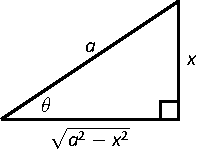
\includegraphics{figures/figtrigsub_intro1}
		\end{minipage}
		
	\item[(b)] \noindent
	\begin{minipage}[t]{.6\linewidth}
		For integrands containing $\sqrt{x^2+a^2}$:\\[5pt]
		Let $x=a\tan\theta$, \qquad $dx = a\sec^2\theta\ d\theta$\\[5pt]	
	Thus $\theta = \tan^{-1}(x/a)$, for $-\pi/2 < \theta < \pi/2$. \\[5pt]	
	On this interval, $\sec\theta> 0$, so\\[5pt]	
	$\sqrt{x^2+a^2} = a\sec\theta$
		\end{minipage}\qquad
	\begin{minipage}[t]{.4\linewidth}\vskip 0pt
		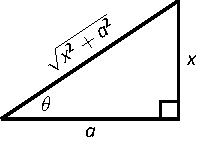
\includegraphics{figures/figtrigsub_intro3}
		\end{minipage}
		
	\item[(c)] \noindent
	\begin{minipage}[t]{.6\linewidth}
		For integrands containing $\sqrt{x^2-a^2}$:\\[5pt]
		Let $x=a\sec\theta$, \qquad $dx = a\sec\theta\tan\theta\ d\theta$\\[5pt]	
	Thus $\theta = \sec^{-1}(x/a)$. If $x/a\geq 1$, then $0\leq\theta<\pi/2$; if $x/a \leq -1$, then $\pi/2<\theta\leq \pi$.\\[5pt]	
	We restrict our work to where $x\geq a$, so $x/a\geq 1$, and $0\leq\theta<\pi/2$.
	On this interval, $\tan\theta\geq 0$, so\\[5pt]	
	$\sqrt{x^2-a^2} = a\tan\theta$
		\end{minipage}\qquad
	\begin{minipage}[t]{.4\linewidth}\vskip 0pt
		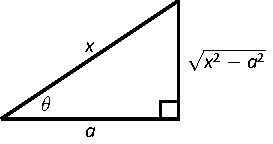
\includegraphics{figures/figtrigsub_intro2}
		\end{minipage}	
\end{enumerate}
}
\end{minipage}
\restoreboxwidth
\vskip \baselineskip

\example{ex_trigsub3}{Using Trigonometric Substitution}{
Evaluate $\ds \int \frac{1}{\sqrt{5+x^2}}\ dx.$}
{Using Key Idea \ref{idea:trigsub}(b), we recognize $a=\sqrt{5}$ and  set $x= \sqrt{5}\tan \theta$. This makes $dx = \sqrt{5}\sec^2\theta\ d\theta$. We will use the fact that $\sqrt{5+x^2} = \sqrt{5+5\tan^2\theta} = \sqrt{5\sec^2\theta} = \sqrt{5}\sec\theta.$ Substituting, we have:
\begin{align*}
\int \frac{1}{\sqrt{5+x^2}}\ dx &= \int \frac{1}{\sqrt{5+5\tan^2\theta}}\sqrt{5}\sec^2\theta\ d\theta \\
			&= \int \frac{\sqrt{5}\sec^2\theta}{\sqrt{5}\sec\theta} \ d\theta\\
			&= \int \sec\theta\ d\theta\\
			&= \ln\big|\sec\theta+\tan\theta\big|+C.
\end{align*}
While the integration steps are over, we are not yet done. The original problem was stated in terms of $x$, whereas our answer is given in terms of $\theta$. We must convert back to $x$.

The reference triangle given in Key Idea \ref{idea:trigsub}(b) helps. With $x=\sqrt{5}\tan\theta$, we have 
$$\tan \theta = \frac x{\sqrt{5}}\quad \text{and}\quad \sec\theta = \frac{\sqrt{x^2+5}}{\sqrt{5}}.$$
This gives
\begin{align*}
\int \frac{1}{\sqrt{5+x^2}}\ dx &= \ln\big|\sec\theta+\tan\theta\big|+C \\
     &= \ln\left|\frac{\sqrt{x^2+5}}{\sqrt{5}}+ \frac x{\sqrt{5}}\right|+C.
\end{align*}
We can leave this answer as is, or we can use a logarithmic identity to simplify it. Note:
\begin{align*}
\ln\left|\frac{\sqrt{x^2+5}}{\sqrt{5}}+ \frac x{\sqrt{5}}\right|+C &= \ln\left|\frac{1}{\sqrt{5}}\big(\sqrt{x^2+5}+ x\big)\right|+C \\
   &= \ln\left|\frac{1}{\sqrt{5}}\right| + \ln\big|\sqrt{x^2+5}+ x\big|+C\\
	&=	\ln\big|\sqrt{x^2+5}+ x\big|+C,
\end{align*}
where the $\ln\big(1/\sqrt{5}\big)$ term is absorbed into the constant $C$. (In Section \ref{sec:hyperbolic} we will learn another way of approaching this problem.)
}\\

\example{ex_trigsub2}{Using Trigonometric Substitution}{
Evaluate $\ds \int \sqrt{4x^2-1}\ dx$.}
{We start by rewriting the integrand so that it looks like $\sqrt{x^2-a^2}$ for some value of $a$:
\begin{align*}
\sqrt{4x^2-1} &= \sqrt{4\left(x^2-\frac14\right)}\\
		&= 2\sqrt{x^2-\left(\frac12\right)^2}.
\end{align*}
So we have $a=1/2$, and following Key Idea \ref{idea:trigsub}(c), we set $x= \frac12\sec\theta$, and hence $dx = \frac12\sec\theta\tan\theta\ d\theta$. %The Key Idea also shows that $\sqrt{x^2-1/2^2} = \frac12\tan\theta$. 
We now rewrite the integral with these substitutions:
\begin{align*}
\int \sqrt{4x^2-1}\ dx &= \int 2\sqrt{x^2-\left(\frac12\right)^2}\ dx\\
			&= \int 2\sqrt{\frac14\sec^2\theta - \frac14}\left(\frac12\sec\theta\tan\theta\right)\ d\theta\\
			&=\int \sqrt{\frac14(\sec^2\theta-1)}\Big(\sec\theta\tan\theta\Big)\ d\theta\\
			&=\int\sqrt{\frac14\tan^2\theta}\Big(\sec\theta\tan\theta\Big)\ d\theta\\
			&=\int \frac12\tan^2\theta\sec\theta\ d\theta\\
			&=\frac12\int \Big(\sec^2\theta-1\Big)\sec\theta\ d\theta\\
			&=\frac12\int \big(\sec^3\theta - \sec\theta\big)\ d\theta.
\end{align*}
We integrated $\sec^3\theta$ in Example \ref{ex_trigint6}, finding its antiderivatives to be
$$\int \sec^3\theta\ d\theta = \frac12\Big(\sec \theta\tan \theta + \ln|\sec \theta+\tan \theta|\Big)+C.$$
\enlargethispage{2\baselineskip}
Thus
\begin{align*}
\int \sqrt{4x^2-1}\ dx &=\frac12\int \big(\sec^3\theta - \sec\theta\big)\ d\theta\\
			&= \frac12\left(\frac12\Big(\sec \theta\tan \theta + \ln|\sec \theta+\tan \theta|\Big) -\ln|\sec \theta + \tan\theta|\right) + C\\
			%\end{align*}
			%\begin{align*}
			&= \frac14\left(\sec\theta\tan\theta -\ln|\sec\theta+\tan\theta|\right)+C.
\end{align*}
We are not yet done. Our original integral is given in terms of $x$, whereas our final answer, as given, is in terms of $\theta$. We need to rewrite our answer in terms of $x$. With $a=1/2$, and $x=\frac12\sec\theta$, the reference triangle in Key Idea \ref{idea:trigsub}(c) shows that 
$$\tan \theta = \sqrt{x^2-1/4}\Big/(1/2) = 2\sqrt{x^2-1/4}\quad \text{and}\quad \sec\theta = 2x.$$
Thus\small 
\begin{align*}
\frac14\Big(\sec\theta\tan\theta -\ln\big|\sec\theta+\tan\theta\big|\Big)+C &=
				\frac14\Big(2x\cdot 2\sqrt{x^2-1/4} - \ln\big|2x + 2\sqrt{x^2-1/4}\big|\Big)+C\\
				&= \frac14\Big(4x\sqrt{x^2-1/4} - \ln\big|2x + 2\sqrt{x^2-1/4}\big|\Big)+C.
\end{align*}
\normalsize 
The final answer is given in the last line above, repeated here:
$$\int \sqrt{4x^2-1}\ dx = \frac14\Big(4x\sqrt{x^2-1/4} - \ln\big|2x + 2\sqrt{x^2-1/4}\big|\Big)+C.$$
}\\

\example{ex_trigsub4}{Using Trigonometric Substitution}{
Evaluate $\ds \int \frac{\sqrt{4-x^2}}{x^2}\ dx$.}
{We use Key Idea \ref{idea:trigsub}(a) with $a=2$, $x=2\sin \theta$, $dx = 2\cos \theta$ and hence $\sqrt{4-x^2} = 2\cos\theta$. This gives
\begin{align*}
\int \frac{\sqrt{4-x^2}}{x^2}\ dx &= \int \frac{2\cos\theta}{4\sin^2\theta}(2\cos\theta)\ d\theta\\
		&= \int \cot^2\theta\ d\theta\\
		&=	\int (\csc^2\theta -1)\ d\theta\\
		&= -\cot\theta -\theta + C.
\end{align*}
We need to rewrite our answer in terms of $x$. Using the reference triangle found in Key Idea \ref{idea:trigsub}(a), we have $\cot\theta = \sqrt{4-x^2}/x$ and $\theta = \sin^{-1}(x/2)$. Thus
$$\int \frac{\sqrt{4-x^2}}{x^2}\ dx = -\frac{\sqrt{4-x^2}}x-\sin^{-1}\left(\frac x2\right) + C.$$
}\\

Trigonometric Substitution can be applied in many situations, even those not of the form $\sqrt{a^2-x^2}$, $\sqrt{x^2-a^2}$ or $\sqrt{x^2+a^2}$. In the following example, we apply it to an integral we already know how to handle.\\

\example{ex_trigsub5}{Using Trigonometric Substitution}{
Evaluate $\ds \int\frac1{x^2+1}\ dx$.}
{We know the answer already as $\tan^{-1}x+C$. We apply Trigonometric Substitution here to show that we get the same answer without inherently relying on knowledge of the derivative of the arctangent function.

Using Key Idea \ref{idea:trigsub}(b), let $x=\tan\theta$, $dx=\sec^2\theta\ d\theta$ and note that $x^2+1 = \tan^2\theta+1 = \sec^2\theta$. Thus
\begin{align*}
\int \frac1{x^2+1}\ dx &= \int \frac{1}{\sec^2\theta}\sec^2\theta\ d\theta \\
			&= \int 1\ d\theta\\
			&= \theta + C.
\end{align*}
Since $x=\tan \theta$, $\theta = \tan^{-1}x$, and we conclude that $\ds \int\frac1{x^2+1}\ dx = \tan^{-1}x+C.$
}\\

The next example is similar to the previous one in that it does not involve a square--root. It shows how several techniques and identities can be combined to obtain a solution.\\

\example{ex_trigsub7}{Using Trigonometric Substitution}{
Evaluate $\ds\int\frac1{(x^2+6x+10)^2}\ dx.$
}
{We start by completing the square, then make the substitution $u=x+3$, followed by the trigonometric substitution of $u=\tan\theta$:
\begin{align}
\int \frac1{(x^2+6x+10)^2}\ dx =\int \frac1{\big((x+3)^2+1\big)^2}\ dx&= \int \frac1{(u^2+1)^2}\ du. \notag
\intertext{Now make the substitution $u=\tan\theta$, $du=\sec^2\theta\ d\theta$:}
   &=	\int \frac1{(\tan^2\theta+1)^2}\sec^2\theta\ d\theta\notag\\
	&= \int\frac 1{(\sec^2\theta)^2}\sec^2\theta\ d\theta\notag\\
	&= \int \cos^2\theta\ d\theta.\notag
	\intertext{Applying a power reducing formula, we have}
	&= \int \left(\frac12 +\frac12\cos(2\theta)\right)\ d\theta \notag\\
	&= \frac12\theta + \frac14\sin(2\theta) + C.\label{eq:extrigsub7}
\end{align}
We need to return to the variable $x$. As $u=\tan\theta$, $\theta = \tan^{-1}u$. Using the identity $\sin(2\theta) = 2\sin\theta\cos\theta$ and using the reference triangle found in Key Idea \ref{idea:trigsub}(b), we have 
$$\frac14\sin(2\theta) = \frac12\frac u{\sqrt{u^2+1}}\cdot\frac 1{\sqrt{u^2+1}} = \frac12\frac u{u^2+1}.$$
Finally, we return to $x$ with the substitution $u=x+3$. We start with the expression in Equation \eqref{eq:extrigsub7}:
\begin{align*}
\frac12\theta + \frac14\sin(2\theta) + C &= \frac12\tan^{-1}u + \frac12\frac{u}{u^2+1}+C\\
				&= \frac12\tan^{-1}(x+3) + \frac{x+3}{2(x^2+6x+10)}+C.
\end{align*}
Stating our final result in one line,
$$\int\frac1{(x^2+6x+10)^2}\ dx=\frac12\tan^{-1}(x+3) + \frac{x+3}{2(x^2+6x+10)}+C.$$
}\\


Our last example returns us to definite integrals, as seen in our first example. Given a definite integral that can be evaluated using Trigonometric Substitution, we could first evaluate the corresponding indefinite integral (by changing from an integral in terms of $x$ to one in terms of $\theta$, then converting back to $x$) and then evaluate using the original bounds. It is much more straightforward, though, to change the bounds as we substitute.\\

\example{ex_trigsub6}{Definite integration and Trigonometric Substitution}{
Evaluate $\ds\int_0^5\frac{x^2}{\sqrt{x^2+25}}\ dx$.
}
{Using Key Idea \ref{idea:trigsub}(b), we set $x=5\tan\theta$, $dx = 5\sec^2\theta\ d\theta$, and note that $\sqrt{x^2+25} = 5\sec\theta$. As we substitute, we can also change the bounds of integration.

The lower bound of the original integral is $x=0$. As $x=5\tan\theta$, we solve for $\theta$ and find $\theta = \tan^{-1}(x/5)$. Thus the new lower bound is $\theta = \tan^{-1}(0) = 0$. The original upper bound is $x=5$, thus the new upper bound is $\theta = \tan^{-1}(5/5) = \pi/4$. 

Thus we have 
\begin{align*}
\int_0^5\frac{x^2}{\sqrt{x^2+25}}\ dx &= \int_0^{\pi/4} \frac{25\tan^2\theta}{5\sec\theta}5\sec^2\theta\ d\theta\\
		&= 25\int_0^{\pi/4} \tan^2\theta\sec\theta\ d\theta.
\end{align*}
We encountered this indefinite integral in Example \ref{ex_trigsub2} where we found 
$$\int \tan^2\theta\sec\theta \ d\theta = \frac12\big(\sec\theta\tan\theta-\ln|\sec\theta+\tan\theta|\big).$$
So
\begin{align*}
25\int_0^{\pi/4} \tan^2\theta\sec\theta\ d\theta &= \frac{25}2\big(\sec\theta\tan\theta-\ln|\sec\theta+\tan\theta|\big)\Bigg|_0^{\pi/4}\\
&= \frac{25}2\big(\sqrt2-\ln(\sqrt2+1)\big)\\
&\approx 6.661.
\end{align*}
\vskip-1.5\baselineskip
}\\

\enlargethispage{3\baselineskip}
The following equalities are very useful when evaluating integrals using Trigonometric Substitution. 

\keyidea{idea:useful_trigsub}{Useful Equalities with Trigonometric Substitution}
{\begin{enumerate}
	\item	$\sin(2\theta) = 2\sin\theta\cos\theta$
	\item	$\cos(2\theta) = \cos^2\theta - \sin^2\theta = 2\cos^2\theta-1 = 1-2\sin^2\theta$
	\item $\ds \int \sec^3\theta\ d\theta = \frac12\Big(\sec \theta\tan \theta + \ln\big|\sec \theta+\tan \theta\big|\Big)+C$
	\item	$\ds \int \cos^2\theta\ d\theta = \int \frac12\big(1+\cos(2\theta)\big)\ d\theta = \frac12\big(\theta+\sin\theta\cos\theta\big)+C.$
\end{enumerate}
}

The next section introduces Partial Fraction Decomposition, which is an algebraic technique that turns ``complicated'' fractions into sums of ``simpler'' fractions, making integration easier.

\printexercises{exercises/06_08_exercises}




%\section{Partial Fraction Decomposition}\label{sec:partial_fraction}

In this section we investigate the antiderivatives of rational functions. Recall that rational functions are functions of the form $f(x)= \frac{p(x)}{q(x)}$, where $p(x)$ and $q(x)$ are polynomials and $q(x)\neq 0$. Such functions arise in many contexts, one of which is the solving of certain fundamental differential equations.

We begin with an example that demonstrates the motivation behind this section. Consider the integral $\ds\int \frac{1}{x^2-1}\ dx$. We do not have a simple formula for this (if the denominator were $x^2+1$, we would recognize the antiderivative as being the arctangent function). It can be solved using Trigonometric Substitution, but note how the integral is easy to evaluate once we realize:

%This integral is not difficult to evaluate once one realizes the following fact: 
$$\frac{1}{x^2-1} = \frac{1/2}{x-1} - \frac{1/2}{x+1}.$$
Thus 
\begin{align*}
\int\frac{1}{x^2-1}\ dx &= \int\frac{1/2}{x-1}\ dx - \int\frac{1/2}{x+1}\ dx \\
			&= \frac12\ln|x-1| - \frac12\ln|x+1| + C.
\end{align*}

This section teaches how to \textit{decompose} $$\frac{1}{x^2-1}\quad  \text{into}\quad  \frac{1/2}{x-1}-\frac{1/2}{x+1}.$$

We start with a rational function $f(x)=\frac{p(x)}{q(x)}$, where $p$ and $q$ do not have any common factors and the degree of $p$ is less than the degree of $q$. It can be shown that any polynomial, and hence $q$, can be factored into a product of linear and irreducible quadratic terms. The following Key Idea states how to decompose a rational function into a sum of rational functions whose denominators are all of lower degree than $q$.
%\clearpage

\keyidea{idea:partial_fraction}{Partial Fraction Decomposition}
{Let $\ds \frac{p(x)}{q(x)}$ be a rational function, where the degree of $p$ is less than the degree of $q$.\index{integration!partial fraction decomp.}
\begin{enumerate}
	\item	\textbf{Linear Terms:} Let $(x-a)$ divide $q(x)$, where $(x-a)^n$ is the highest power of $(x-a)$ that divides $q(x)$. Then the decomposition of $\frac{p(x)}{q(x)}$ will contain the sum
	$$\frac{A_1}{(x-a)} + \frac{A_2}{(x-a)^2} + \cdots +\frac{A_n}{(x-a)^n}.$$
	\item		\textbf{Quadratic Terms:} Let $x^2+bx+c$ divide $q(x)$, where $(x^2+bx+c)^n$ is the highest power of $x^2+bx+c$ that divides $q(x)$. Then the decomposition of $\frac{p(x)}{q(x)}$ will contain the sum 
	$$\frac{B_1x+C_1}{x^2+bx+c}+\frac{B_2x+C_2}{(x^2+bx+c)^2}+\cdots+\frac{B_nx+C_n}{(x^2+bx+c)^n}.$$
	\end{enumerate}
	To find the coefficients $A_i$, $B_i$ and $C_i$:
	\begin{enumerate}
	\item	Multiply all fractions by $q(x)$, clearing the denominators. Collect like terms.
	\item		Equate the resulting coefficients of the powers of $x$ and solve the resulting system of linear equations.
	\end{enumerate}
}

The following examples will demonstrate how to put this Key Idea into practice. Example \ref{ex_pf1} stresses the decomposition aspect of the Key Idea.\\

\example{ex_pf1}{Decomposing into partial fractions}{
Decompose $\ds f(x)=\frac{1}{(x+5)(x-2)^3(x^2+x+2)(x^2+x+7)^2}$ without solving for the resulting coefficients.}
{The denominator is already factored, as both $x^2+x+2$ and $x^2+x+7$ cannot be factored further. We need to decompose $f(x)$ properly. Since $(x+5)$ is a linear term that divides the denominator, there will be a $$\frac{A}{x+5}$$ term in the decomposition.

As $(x-2)^3$ divides the denominator, we will have the following terms in the decomposition:
$$\frac{B}{x-2},\quad \frac{C}{(x-2)^2}\quad \text{and}\quad \frac{D}{(x-2)^3}.$$

The $x^2+x+2$ term in the denominator results in a $\ds\frac{Ex+F}{x^2+x+2}$ term.

Finally, the $(x^2+x+7)^2$ term results in the terms $$\frac{Gx+H}{x^2+x+7}\quad \text{and}\quad \frac{Ix+J}{(x^2+x+7)^2}.$$
All together, we have 
\begin{align*}
\frac{1}{(x+5)(x-2)^3(x^2+x+2)(x^2+x+7)^2} &= \frac{A}{x+5} + \frac{B}{x-2}+ \frac{C}{(x-2)^2}+\frac{D}{(x-2)^3}+ \\
		& \frac{Ex+F}{x^2+x+2}+\frac{Gx+H}{x^2+x+7}+\frac{Ix+J}{(x^2+x+7)^2}
\end{align*}
Solving for the coefficients $A$, $B \ldots J$ would be a bit tedious but not ``hard.''
}\\

\example{ex_pf2}{Decomposing into partial fractions}{
Perform the partial fraction decomposition of $\ds \frac{1}{x^2-1}$.}
{The denominator factors into two linear terms: $x^2-1 = (x-1)(x+1)$. Thus 
$$\frac{1}{x^2-1} = \frac{A}{x-1} + \frac{B}{x+1}.$$
To solve for $A$ and $B$, first multiply through by $x^2-1 = (x-1)(x+1)$:
\begin{align*}
1 &= \frac{A(x-1)(x+1)}{x-1}+\frac{B(x-1)(x+1)}{x+1} \\
	&= A(x+1) + B(x-1)\\
	&= Ax+A + Bx-B \\
	\intertext{Now collect like terms.}
	&= (A+B)x + (A-B).
\end{align*}
The next step is key. Note the equality we have:
$$1 = (A+B)x+(A-B).$$
For clarity's sake, rewrite the left hand side as
$$0x+1 = (A+B)x+(A-B).$$
On the left, the coefficient of the $x$ term is 0; on the right, it is $(A+B)$. Since both sides are equal, we must have that $0=A+B$. 

Likewise, on the left, we have a constant term of 1; on the right, the constant term is $(A-B)$. Therefore we have $1=A-B$.

We have two linear equations with two unknowns. This one is easy to solve by hand, leading to 
$$\begin{array}{c} A+B = 0 \\ A-B = 1 \end{array} \Rightarrow \begin{array}{c} A=1/2 \\ B = -1/2\end{array}.$$
Thus $$\frac{1}{x^2-1} = \frac{1/2}{x-1}-\frac{1/2}{x+1}.$$
\vskip-\baselineskip
}\\

\example{ex_pf3}{Integrating using partial fractions}{
Use partial fraction decomposition to integrate $\ds\int\frac{1}{(x-1)(x+2)^2}\ dx.$}
{We decompose the integrand as follows, as described by Key Idea \ref{idea:partial_fraction}:
$$\frac{1}{(x-1)(x+2)^2} = \frac{A}{x-1} + \frac{B}{x+2} + \frac{C}{(x+2)^2}.$$
To solve for $A$, $B$ and $C$, we multiply both sides by $(x-1)(x+2)^2$ and collect like terms:
\begin{align}
1 &= A(x+2)^2 + B(x-1)(x+2) + C(x-1)\label{eq:pf3}\\
	&= Ax^2+4Ax+4A + Bx^2 + Bx-2B + Cx-C \notag \\
	&= (A+B)x^2 + (4A+B+C)x + (4A-2B-C)\notag
\end{align}
\mnote{.5}{\textbf{Note:} Equation \ref{eq:pf3} offers a direct route to finding the values of $A$, $B$ and $C$. Since the equation holds for all values of $x$, it holds in particular when $x=1$. However, when $x=1$, the right hand side simplifies to $A(1+2)^2 = 9A$. Since the left hand side is still 1, we have $1 = 9A$. Hence $A = 1/9$.

Likewise, the equality holds when $x=-2$; this leads to the equation $1=-3C$. Thus $C = -1/3$.

Knowing $A$ and $C$, we can find the value of $B$ by choosing yet another value of $x$, such as $x=0$, and solving for $B$.}
We have $$0x^2+0x+ 1 = (A+B)x^2 + (4A+B+C)x + (4A-2B-C)$$
leading to the equations 
$$A+B = 0, \quad 4A+B+C = 0 \quad \text{and} \quad 4A-2B-C = 1.$$
These three equations of three unknowns lead to a unique solution:
$$A = 1/9,\quad B = -1/9 \quad \text{and} \quad C = -1/3.$$
Thus 
$$\int\frac{1}{(x-1)(x+2)^2}\ dx = \int \frac{1/9}{x-1}\ dx + \int \frac{-1/9}{x+2}\ dx + \int \frac{-1/3}{(x+2)^2}\ dx.$$

Each can be integrated with a simple substitution with $u=x-1$ or $u=x+2$ (or by directly applying Key Idea \ref{idea:linearsub} as the denominators are linear functions). The end result is
$$\int\frac{1}{(x-1)(x+2)^2}\ dx = \frac19\ln|x-1| -\frac19\ln|x+2| +\frac1{3(x+2)}+C.$$
\vskip-\baselineskip}\\

%\enlargethispage{\baselineskip}
\example{ex_pf4}{Integrating using partial fractions}{
Use partial fraction decomposition to integrate $\ds \int \frac{x^3}{(x-5)(x+3)}\ dx$.}
{Key Idea \ref{idea:partial_fraction} presumes that the degree of the numerator is less than the degree of the denominator. Since this is not the case here, we begin by using polynomial division to reduce the degree of the numerator. We omit the steps, but encourage the reader to verify that $$\frac{x^3}{(x-5)(x+3)} = x+2+\frac{19x+30}{(x-5)(x+3)}.$$
Using Key Idea \ref{idea:partial_fraction}, we can rewrite the new rational function as:
$$\frac{19x+30}{(x-5)(x+3)} = \frac{A}{x-5} + \frac{B}{x+3}$$ for appropriate values of $A$ and $B$. Clearing denominators, we have 

\mnote{.6}{\textbf{Note:} The values of $A$ and $B$ can be quickly found using the technique described in the margin of Example \ref{ex_pf3}.}

\begin{align*}
19x+30 &= A(x+3) + B(x-5)\\
			&= (A+B)x + (3A-5B).
\intertext{This implies that:}
19&= A+B \\
30&= 3A-5B.\\
\intertext{Solving this system of linear equations gives}
125/8 &=A\\
27/8 &=B.
\end{align*}

We can now integrate.
\begin{align*}
\int \frac{x^3}{(x-5)(x+3)}\ dx &= \int\left(x+2+\frac{125/8}{x-5}+\frac{27/8}{x+3}\right)\ dx \\
					&= \frac{x^2}2 + 2x + \frac{125}{8}\ln|x-5| + \frac{27}8\ln|x+3| + C.
\end{align*}
\vskip-\baselineskip
}\\
%\clearpage

\example{ex_pf5}{Integrating using partial fractions}{
Use partial fraction decomposition to evaluate $\ds \int\frac{7x^2+31x+54}{(x+1)(x^2+6x+11)}\ dx.$}
{The degree of the numerator is less than the degree of the denominator so we begin by applying Key Idea \ref{idea:partial_fraction}. We have:
\begin{align*}
\frac{7x^2+31x+54}{(x+1)(x^2+6x+11)} &= \frac{A}{x+1} + \frac{Bx+C}{x^2+6x+11}. \\
\intertext{Now clear the denominators.}
7x^2+31x+54 &= A(x^2+6x+11) + (Bx+C)(x+1)\\
					&= (A+B)x^2 + (6A+B+C)x + (11A+C).\\
\intertext{This implies that:}
				7&=A+B\\
				31 &= 6A+B+C\\
				54 &= 11A+C.
\end{align*}
Solving this system of linear equations gives the nice result of $A=5$, $B = 2$ and $C=-1$. Thus
$$\int\frac{7x^2+31x+54}{(x+1)(x^2+6x+11)}\ dx = \int\left(\frac{5}{x+1} + \frac{2x-1}{x^2+6x+11}\right)\ dx.$$

The first term of this new integrand is easy to evaluate; it leads to a $5\ln|x+1|$ term. The second term is not hard, but takes several steps and uses substitution techniques.

The integrand $\ds \frac{2x-1}{x^2+6x+11}$ has a quadratic in the denominator and a linear term in the numerator. This leads us to try substitution. Let $u = x^2+6x+11$, so $du = (2x+6)\ dx$. The numerator is $2x-1$, not $2x+6$, but we can get a $2x+6$ term in the numerator by adding 0 in the form of ``$7-7$.''
\begin{align*}
\frac{2x-1}{x^2+6x+11} &= \frac{2x-1+7-7}{x^2+6x+11} \\
					&= \frac{2x+6}{x^2+6x+11} - \frac{7}{x^2+6x+11}.
\end{align*}
We can now integrate the first term with substitution, leading to a $\ln|x^2+6x+11|$ term. The final term can be integrated using arctangent. First, complete the square in the denominator:
$$\frac{7}{x^2+6x+11} = \frac{7}{(x+3)^2+2}.$$
An antiderivative of the latter term can be found using Theorem \ref{thm:int_inverse_trig} and substitution:
$$\int \frac{7}{x^2+6x+11}\ dx = \frac{7}{\sqrt{2}}\tan^{-1}\left(\frac{x+3}{\sqrt{2}}\right)+C.$$

Let's start at the beginning and put all of the steps together.
\small\begin{align*}
\int\frac{7x^2+31x+54}{(x+1)(x^2+6x+11)}\ dx &= \int\left(\frac{5}{x+1} + \frac{2x-1}{x^2+6x+11}\right)\ dx \\
			&= \int\frac{5}{x+1}\ dx  + \int\frac{2x+6}{x^2+6x+11}\ dx -\int\frac{7}{x^2+6x+11}\ dx \\
			&= 5\ln|x+1|+ \ln|x^2+6x+11| -\frac{7}{\sqrt{2}}\tan^{-1}\left(\frac{x+3}{\sqrt{2}}\right)+C.
\end{align*}\normalsize
As with many other problems in calculus, it is important to remember that one is not expected to ``see'' the final answer immediately after seeing the problem. Rather, given the initial problem, we break it down into smaller problems that are easier to solve. The final answer is a combination of the answers of the smaller problems.
}\\

Partial Fraction Decomposition is an important tool when dealing with rational functions. Note that at its heart, it is a technique of algebra, not calculus, as we are rewriting a fraction in a new form. Regardless, it is very useful in the realm of calculus as it lets us evaluate a certain set of ``complicated'' integrals.

The next section introduces new functions, called the Hyperbolic Functions. They will allow us to make substitutions similar to those found when studying Trigonometric Substitution, allowing us to approach even more integration problems. 


\printexercises{exercises/06_04_exercises}
%\section{Hyperbolic Functions}\label{sec:hyperbolic}

The \textbf{hyperbolic functions} are a set of functions that have many applications to mathematics, physics, and engineering. Among many other applications, they are used to describe the formation of satellite rings around planets, to describe the shape of a rope hanging from two points, and have application to the theory of special relativity. This section defines the hyperbolic functions and describes many of their properties, especially their usefulness to calculus.

These functions are sometimes referred to as the ``hyperbolic trigonometric functions'' as there are many, many connections between them and the standard trigonometric functions. Figure \ref{fig:hfcircle} demonstrates one such connection. Just as cosine and sine are used to define points on the circle defined by $x^2+y^2=1$, the functions \textbf{hyperbolic cosine} and \textbf{hyperbolic sine} are used to define points on the hyperbola $x^2-y^2=1$.

\mtable{.7}{Using trigonometric functions to define points on a circle and hyperbolic functions to define points on a hyperbola. The area of the shaded regions are included in them.}{fig:hfcircle}{\myincludegraphics{figures/fighf_circlearea}\vskip10pt\myincludegraphics{figures/fighf_hyperbolaarea}}

We begin with their definition.

\definition{def:hyperbolic_functions}{Hyperbolic Functions}
{\noindent%
\begin{minipage}{.5\specialboxlength}
\begin{enumerate}
\item		$\ds \cosh x = \frac{e^x+e^{-x}}2$\index{hyperbolic function!definition}
\item		$\ds \sinh x = \frac{e^x-e^{-x}}2$
\item		$\ds \tanh x = \frac{\sinh x}{\cosh x}$
\end{enumerate}
\end{minipage}
\begin{minipage}{.5\specialboxlength}
\begin{enumerate}\addtocounter{enumi}{3}
\item		$\ds \sech x = \frac{1}{\cosh x}$
\item		$\ds \csch x = \frac{1}{\sinh x}$
\item		$\ds \coth x = \frac{\cosh x}{\sinh x}$
\end{enumerate}
\end{minipage}
}\\

These hyperbolic functions are graphed in Figure \ref{fig:hyperbolic}. In the graphs of $\cosh x$ and $\sinh x$, graphs of $e^x/2$ and $e^{-x}/2$ are included with dashed lines. As $x$ gets ``large,'' $\cosh x$ and $\sinh x$ each act like $e^x/2$; when $x$ is a large negative number, $\cosh x$ acts like $e^{-x}/2$ whereas $\sinh x$ acts like $-e^{-x}/2$.

Notice the domains of $\tanh x$ and $\sech x$ are $(-\infty,\infty)$, whereas both $\coth x$ and $\csch x$ have vertical asymptotes at $x=0$. Also note the ranges of these functions, especially $\tanh x$: as $x\to\infty$, both $\sinh x$ and $\cosh x$ approach $e^{x}/2$, hence $\tanh x$ approaches $1$.

%It is no coincidence that these functions share a name similar to the trigonometric functions. 
The following example explores some of the properties of these functions that bear remarkable resemblance to the properties of their trigonometric counterparts.\\

\mnote{.4}{\textbf{Pronunciation Note:} \par 
``cosh'' rhymes with ``gosh,'' \par ``sinh'' rhymes with ``pinch,'' and \par ``tanh'' rhymes with ``ranch.''}

\clearpage
\begin{center}
\begin{tabular}{ccc}
\myincludegraphics{figures/fighf_cosh} &\ \hskip 25pt\ & \myincludegraphics{figures/fighf_sinh} \\[20pt]
\myincludegraphics{figures/fighf_tanh_coth}& &\myincludegraphics{figures/fighf_sech_csch}
\end{tabular}
\captionsetup{type=figure}
\caption{Graphs of the hyperbolic functions.}\label{fig:hyperbolic}
\end{center}
\vskip\baselineskip
\enlargethispage{2\baselineskip}


\example{ex_hf1}{Exploring properties of hyperbolic functions}{
\noindent Use Definition \ref{def:hyperbolic_functions} to rewrite the following expressions.

\noindent\begin{minipage}{.5\linewidth}
\begin{enumerate}
\item		$\cosh^2 x-\sinh^2x$
\item		$\tanh^2 x+\sech^2 x$
\item		$2\cosh x\sinh x$
\end{enumerate}
\end{minipage}
\begin{minipage}{.5\linewidth}
\begin{enumerate}\addtocounter{enumi}{3}
\item		$\frac{d}{dx}\big(\cosh x\big)$
\item		$\frac{d}{dx}\big(\sinh x\big)$
\item		$\frac{d}{dx}\big(\tanh x\big)$
\end{enumerate}
\end{minipage}
}
{\begin{enumerate}
\item		%\vskip-\baselineskip%
\hfill$\begin{aligned}[t]
 \cosh^2x-\sinh^2x &= \left(\frac{e^x+e^{-x}}2\right)^2 -\left(\frac{e^x-e^{-x}}2\right)^2\\
 						&= \frac{e^{2x}+2e^xe^{-x} + e^{-2x}}4 - \frac{e^{2x}-2e^xe^{-x} + e^{-2x}}4\\
 						&= \frac44=1.
\end{aligned}$\hfill

So $\cosh^2 x-\sinh^2x=1$.

\item		\hfill$\begin{aligned}[t]
\tanh^2 x+\sech^2 x &=\frac{\sinh^2x}{\cosh^2 x} + \frac{1}{\cosh^2 x} \\
					&= \frac{\sinh^2x+1}{\cosh^2 x}\qquad \text{\small Now use identity from \#1.}\\
					&= \frac{\cosh^2 x}{\cosh^2 x} = 1.
\end{aligned}$\hfill

%%% Figure of the hyperbolic functions
%\mtable{.55}{Graphs of the hyperbolic functions.}{fig:hyperbolic}{\myincludegraphics{figures/fighf_cosh}\vskip 10pt \myincludegraphics{figures/fighf_sinh} \vskip 10pt\myincludegraphics{figures/fighf_tanh_coth}\vskip 10pt\myincludegraphics{figures/fighf_sech_csch}}
%%%


So $\tanh^2 x+\sech^2 x=1$.

%\drawexampleline
\enlargethispage{2\baselineskip}

\item \hfill$\begin{aligned}[t]
	2\cosh x\sinh x &= 2\left(\frac{e^x+e^{-x}}2\right)\left(\frac{e^x-e^{-x}}2\right) \\
					&= 2 \cdot\frac{e^{2x} - e^{-2x}}4\\
					&= \frac{e^{2x} - e^{-2x}}2 = \sinh (2x).\\
			\end{aligned}$ \hfill
			
Thus $2\cosh x\sinh x = \sinh (2x)$.

\item  \hfill$\begin{aligned}[t]
	\frac{d}{dx}\big(\cosh x\big) &= \frac{d}{dx}\left(\frac{e^x+e^{-x}}2\right) \\
					&= \frac{e^x-e^{-x}}2\\
					&= \sinh x.
	\end{aligned}\hfill$

So $\frac{d}{dx}\big(\cosh x\big) = \sinh x.$
	
\item  \hfill$\begin{aligned}[t]
	\frac{d}{dx}\big(\sinh x\big) &= \frac{d}{dx}\left(\frac{e^x-e^{-x}}2\right) \\
					&= \frac{e^x+e^{-x}}2\\
					&= \cosh x.
	\end{aligned}\hfill$

So $\frac{d}{dx}\big(\sinh x\big) = \cosh x.$
	
\item  \hfill$\begin{aligned}[t]
	\frac{d}{dx}\big(\tanh x\big) &= \frac{d}{dx}\left(\frac{\sinh x}{\cosh x}\right) \\
					&= \frac{\cosh x \cosh x - \sinh x \sinh x}{\cosh^2 x}\\
					&= \frac{1}{\cosh^2 x}\\
					&= \sech^2 x.
	\end{aligned}\hfill$

So $\frac{d}{dx}\big(\tanh x\big) = \sech^2 x.$	
\end{enumerate}
\vskip-\baselineskip
}\\

The following Key Idea summarizes many of the important identities relating to hyperbolic functions. Each can be verified by referring back to Definition \ref{def:hyperbolic_functions}.

\setboxwidth{160pt}
\noindent\ifthenelse{\isodd{\thepage}}{\hskip -160pt}{}%
\begin{minipage}{\specialboxlength}
\keyidea{idea:hyperbolic_identities}{Useful Hyperbolic Function Properties}
{\begin{minipage}[t]{.33\specialboxlength}
\textbf{Basic Identities}\par
\begin{enumerate}
\item $\cosh^2x-\sinh^2x=1$%
\index{hyperbolic function!identities}\index{hyperbolic function!derivatives}\index{hyperbolic function!integrals}\index{derivative!hyperbolic funct.}\index{integration!hyperbolic funct.}%
\item	$\tanh^2x+\sech^2x=1$
\item	$\coth^2x-\csch^2x = 1$
\item	$\cosh 2x=\cosh^2x+\sinh^2x$
\item	$\sinh 2x = 2\sinh x\cosh x$
\item	$\ds\cosh^2x = \frac{\cosh 2x+1}{2}$
\item $\ds \sinh^2x=\frac{\cosh 2x-1}{2}$
\end{enumerate}
\end{minipage}
\begin{minipage}[t]{.33\specialboxlength}
\textbf{Derivatives}
\begin{enumerate}
\item $\frac{d}{dx}\big(\cosh x\big) = \sinh x$
\item $\frac{d}{dx}\big(\sinh x\big) = \cosh x$
\item $\frac{d}{dx}\big(\tanh x\big) = \sech^2 x$
\item $\frac{d}{dx}\big(\sech x\big) = -\sech x\tanh x$
\item $\frac{d}{dx}\big(\csch x\big) = -\csch x\coth x$
\item $\frac{d}{dx}\big(\coth x\big) = -\csch^2x$
\end{enumerate}
\end{minipage}
\begin{minipage}[t]{.33\specialboxlength}
\textbf{Integrals}
\begin{enumerate}
\item $\ds\int \cosh x\ dx = \sinh x+C$
\item $\ds\int \sinh x\ dx = \cosh x+C$
\item $\ds\int \tanh x\ dx = \ln(\cosh x) +C$
\item $\ds\int \coth x\ dx = \ln|\sinh x\,|+C$
\end{enumerate}
\end{minipage}
}
\end{minipage}
\restoreboxwidth
\\

We practice using Key Idea \ref{idea:hyperbolic_identities}.\\

\example{ex_hf2}{Derivatives and integrals of hyperbolic functions}{Evaluate the following derivatives and integrals.

\begin{minipage}[t]{.5\linewidth}
\begin{enumerate}
\item		$\ds\frac{d}{dx}\big(\cosh 2x\big)$
\item		$\ds\int \sech^2(7t-3)\ dt$
\end{enumerate}
\end{minipage}
\begin{minipage}[t]{.5\linewidth}
\begin{enumerate}\addtocounter{enumi}{2}
\item		$\ds \int_0^{\ln 2} \cosh x\ dx$
\end{enumerate}
\end{minipage}
}
{\begin{enumerate}
\item		Using the Chain Rule directly, we have $\frac{d}{dx} \big(\cosh 2x\big) = 2\sinh 2x$.

Just to demonstrate that it works, let's also use the Basic Identity found in Key Idea \ref{idea:hyperbolic_identities}: $\cosh 2x = \cosh^2x+\sinh^2x$.
\begin{align*}\frac{d}{dx}\big(\cosh 2x\big) = \frac{d}{dx}\big(\cosh^2x+\sinh^2x\big) &= 2\cosh x\sinh x+ 2\sinh x\cosh x\\ &= 4\cosh x\sinh x.
\end{align*}
Using another Basic Identity, we can see that $4\cosh x\sinh x = 2\sinh 2x$. We get the same answer either way.

\item	  We employ substitution, with $u = 7t-3$ and $du = 7dt$. Applying Key Ideas \ref{idea:linearsub}  and \ref{idea:hyperbolic_identities} we have:
$$ \int \sech^2 (7t-3)\ dt = \frac17\tanh (7t-3) + C.$$

\item		$$\int_0^{\ln 2} \cosh x\ dx = \sinh x\Big|_0^{\ln 2} = \sinh (\ln 2) - \sinh 0 = \sinh(\ln 2).$$

We can simplify this last expression as $\sinh x$ is based on exponentials:
$$\sinh(\ln 2) = \frac{e^{\ln 2}-e^{-\ln 2}}2 = \frac{2-1/2}{2} = \frac34.$$
\end{enumerate}
\vskip-1.5\baselineskip
}\\

\noindent\textbf{\large Inverse Hyperbolic Functions}\\

Just as the inverse trigonometric functions are useful in certain integrations, the inverse hyperbolic functions are useful with others. Figure \ref{fig:hfinverse2} shows the restrictions on the domains to make each function one-to-one and the resulting domains and ranges of their inverse functions. Their graphs are shown in Figure \ref{fig:hfinverse1}.\index{hyperbolic function!inverse}

Because the hyperbolic functions are defined in terms of exponential functions, their inverses can be expressed in terms of logarithms as shown in Key Idea \ref{idea:hyperbolic_log}. It is often more convenient to refer to $\sinh^{-1}x$ than to $\ln\big(x+\sqrt{x^2+1}\big)$, especially when one is working on theory and does not need to compute actual values. On the other hand, when computations are needed, technology is often helpful but many hand-held calculators lack a \textit{convenient} $\sinh^{-1}x$ button. (Often it can be accessed under a menu system, but not conveniently.) In such a situation, the logarithmic representation is useful. The reader is not encouraged to memorize these, but rather know they exist and know how to use them when needed.
\clearpage


%\mtable{.7}{Graphs of $\cosh x$, $\sinh x$ and their inverses.}{fig:hfinverse3}{\myincludegraphics{figures/fighfarccosh} \vskip 10pt\myincludegraphics{figures/fighfarcsinh}}
%
%\mtable{.3}{Graphs of $\tanh^{-1} x$, $\coth^{-1} x$, $\sech^{-1} x$ and $\csch^{-1} x$.}{fig:hfinverse4}{\myincludegraphics{figures/fighfarctanharccoth} \vskip 10pt\myincludegraphics{figures/fighfarcsecharccsch}}

%\clearpage

\hskip-.5\textwidth
\noindent\begin{minipage}{1.3\textwidth}
%\centering
\small
\begin{tabular}{ccc}
Function & Domain & Range\\ \hline
$\cosh x$ & $[0,\infty)$ & $[1,\infty)$\\
$\sinh x$ & $(-\infty,\infty)$ & $(-\infty,\infty)$\\
$\tanh x$ & $(-\infty,\infty)$ & $(-1,1)$\\
$\sech x$ & $[0,\infty)$ & $(0,1]$ \\
$\csch x$ & $(-\infty,0) \cup (0,\infty)$ & $(-\infty,0) \cup (0,\infty)$\\
$\coth x$ & $(-\infty,0) \cup (0,\infty)$ & $(-\infty,-1) \cup (1,\infty)$
\end{tabular}
\hskip 40pt
%\end{minipage}\hskip 40pt
%\begin{minipage}{.7\textwidth}
%\centering\small
\begin{tabular}{ccc}
Function & Domain & Range\\ \hline
\rule{0pt}{10pt}$\cosh^{-1} x$ & $[1,\infty)$ & $[0,\infty)$ \\
$\sinh^{-1} x$ & $(-\infty,\infty)$ & $(-\infty,\infty)$\\
$\tanh^{-1} x$ & $(-1,1)$ & $(-\infty,\infty)$\\
$\sech^{-1} x$ & $(0,1]$ & $[0,\infty)$ \\
$\csch^{-1} x$ & $(-\infty,0) \cup (0,\infty)$ & $(-\infty,0) \cup (0,\infty)$\\
$\coth^{-1} x$ & $(-\infty,-1) \cup (1,\infty)$ & $(-\infty,0) \cup (0,\infty)$
\end{tabular}
%\captionsetup{type=figure}%
%\caption{Restricted domains and ranges of the hyperbolic functions.}\label{fig:hfinverse1}
\captionsetup{type=figure}%
\caption{Domains and ranges of the hyperbolic and inverse hyperbolic functions.}\label{fig:hfinverse2}
\end{minipage}
\enlargethispage{3\baselineskip}

\hskip-100pt
\noindent
\begin{minipage}{1.3\textwidth}
\begin{tabular}{ccc}
\myincludegraphics[scale=0.95]{figures/fighfarccosh} & \ \hskip 15pt\ &\myincludegraphics[scale=0.95]{figures/fighfarcsinh}\\[15pt]
\myincludegraphics[scale=0.95]{figures/fighfarctanharccoth} & &\myincludegraphics[scale=0.95]{figures/fighfarcsecharccsch}
\end{tabular}
\captionsetup{type=figure}%
\caption{Graphs of the hyperbolic functions and their inverses.}\label{fig:hfinverse1}
\end{minipage}

\setboxwidth{120pt}
\noindent\hskip-120pt
\begin{minipage}{\specialboxlength}
\keyidea{idea:hyperbolic_log}{Logarithmic definitions of Inverse Hyperbolic Functions}
{\noindent%
\begin{minipage}[t]{.5\specialboxlength}
\begin{enumerate}
\item $\ds\cosh^{-1}x=\ln\big(x+\sqrt{x^2-1}\big);\ x\geq1$\index{hyperbolic function!inverse!logarithmic def.}\rule[-10pt]{0pt}{20pt}
\item $\ds\tanh^{-1}x = \frac12\ln\left(\frac{1+x}{1-x}\right);\ |x|<1$\rule[-10pt]{0pt}{20pt}
\item $\ds \sech^{-1}x = \ln\left(\frac{1+\sqrt{1-x^2}}x\right);\ 0<x\leq1$\rule[-10pt]{0pt}{20pt}
\end{enumerate}
\end{minipage}
\begin{minipage}[t]{.5\specialboxlength}
\begin{enumerate}\addtocounter{enumi}{3}
\item $\ds\sinh^{-1}x = \ln\big(x+\sqrt{x^2+1}\big)$\rule[-10pt]{0pt}{20pt}
\item	 $\ds\coth^{-1}x = \frac12\ln\left(\frac{x+1}{x-1}\right);\ |x|>1$\rule[-10pt]{0pt}{20pt}
\item $\ds\csch^{-1}x = \ln\left(\frac1x+\frac{\sqrt{1+x^2}}{|x|}\right);\ x\neq0$\rule[-10pt]{0pt}{20pt}
\end{enumerate}
\end{minipage}
}
\end{minipage}
\restoreboxwidth

The following Key Ideas give the derivatives and integrals relating to the inverse hyperbolic functions. In Key Idea \ref{idea:hyperbolic_inverse_integrals}, both the inverse hyperbolic and logarithmic function representations of the antiderivative are given, based on Key Idea \ref{idea:hyperbolic_log}. Again, these latter functions are often more useful than the former. Note how inverse hyperbolic functions can be used to solve integrals we used Trigonometric Substitution to solve in Section \ref{sec:trig_sub}.



%\mtable{.62}{Logarithmic definitions of the inverse hyperbolic functions.}{fig:hfinverse5}{%
%\begin{align*}
%\cosh^{-1}x&=\ln\big(x+\sqrt{x^2-1}\big);\ x\geq1\\
%\sinh^{-1}x &= \ln\big(x+\sqrt{x^2+1}\big)\\
%\tanh^{-1}x &= \frac12\ln\left(\frac{1+x}{1-x}\right);\ |x|<1\\
%\sech^{-1}x &= \ln\left(\frac{1+\sqrt{1-x^2}}x\right);\ 0<x\leq1\\
%\csch^{-1}x &= \ln\left(\frac1x+\frac{\sqrt{1+x^2}}{|x|}\right);\ x\neq0\\
%\coth^{-1}x &= \frac12\ln\left(\frac{x+1}{x-1}\right);\ |x|>1
%\end{align*}
%}

\setboxwidth{120pt}
\noindent%\hskip -120pt%
\begin{minipage}{\specialboxlength}
\keyidea{idea:hyperbolic_inverse_derivatives}{Derivatives Involving Inverse Hyperbolic Functions}
{%
\begin{minipage}[t]{.45\specialboxlength}
\begin{enumerate}
\item $\ds\frac{d}{dx}\big(\cosh^{-1} x\big) = \frac{1}{\sqrt{x^2-1}};\ x>1$\index{derivative!inverse hyper.}\index{hyperbolic function!inverse!derivative}
\item $\ds\frac{d}{dx}\big(\sinh^{-1} x\big) = \frac{1}{\sqrt{x^2+1}}$
\item $\ds\frac{d}{dx}\big(\tanh^{-1} x\big) = \frac{1}{1-x^2};\ |x|<1$
\end{enumerate}
\end{minipage}
\begin{minipage}[t]{.55\specialboxlength}
\begin{enumerate}\addtocounter{enumi}{3}
\item $\ds\frac{d}{dx}\big(\sech^{-1} x\big) = \frac{-1}{x\sqrt{1-x^2}}; 0<x<1$
\item $\ds\frac{d}{dx}\big(\csch^{-1} x\big) = \frac{-1}{|x|\sqrt{1+x^2}};\ x\neq0$
\item $\ds\frac{d}{dx}\big(\coth^{-1} x\big) = \frac{1}{1-x^2};\ |x|>1$
\end{enumerate}
\end{minipage}
}
\end{minipage}
\restoreboxwidth
\\

\setboxwidth{120pt}
\noindent%\hskip -120pt%
\begin{minipage}{\specialboxlength}
\keyidea{idea:hyperbolic_inverse_integrals}{Integrals Involving Inverse Hyperbolic Functions}
{%
\begin{enumerate}
\item \parbox{70pt}{$\ds\int \frac{1}{\sqrt{x^2-a^2}}\ dx$} \parbox{180pt}{$\ds=\qquad \cosh^{-1}\left(\frac xa\right)+C;\ 0<a<x$} $\ds=\ln\Big|x+\sqrt{x^2-a^2}\Big|+C$\index{integration!inverse hyper.}\index{hyperbolic function!inverse!integration}

\item \parbox{70pt}{$\ds\int \frac{1}{\sqrt{x^2+a^2}}\ dx$} \parbox{180pt}{$\ds=\qquad \sinh^{-1}\left(\frac xa\right)+C;\ a>0$} $\ds=\ln\Big|x+\sqrt{x^2+a^2}\Big|+C$

\item \parbox{70pt}{$\ds\int \frac{1}{a^2-x^2}\ dx$} \parbox{180pt}{$\ds=\qquad \left\{\begin{array}{ccc} \frac1a\tanh^{-1}\left(\frac xa\right)+C & & x^2<a^2 \\ \\
\frac1a\coth^{-1}\left(\frac xa\right)+C & & a^2<x^2 \end{array}\right.$} $\ds=\frac1{2a}\ln\left|\frac{a+x}{a-x}\right|+C$

\item \parbox{70pt}{$\ds\int \frac{1}{x\sqrt{a^2-x^2}}\ dx $} \parbox{180pt}{$\ds=\qquad -\frac1a\sech^{-1}\left(\frac xa\right)+C;\ 0<x<a$} $\ds= \frac1a \ln\left(\frac{x}{a+\sqrt{a^2-x^2}}\right)+C $

\item	\parbox{70pt}{$\ds\int \frac{1}{x\sqrt{x^2+a^2}}\ dx $} \parbox{180pt}{$\ds=\qquad -\frac1a\csch^{-1}\left|\frac xa\right| + C;\ x\neq 0,\ a>0$}$\ds= \frac1a \ln\left|\frac{x}{a+\sqrt{a^2+x^2}}\right|+C $
\end{enumerate}
%\end{minipage}
}
\end{minipage}
\restoreboxwidth
\\

We practice using the derivative and integral formulas in the following example.\\
\clearpage

\example{ex_hf3}{\parbox[t]{220pt}{Derivatives and integrals involving inverse hyperbolic functions}}
{Evaluate the following.

\noindent%
\begin{minipage}[t]{.5\textwidth}
\begin{enumerate}
\item	$\ds \frac{d}{dx}\left[\cosh^{-1}\left(\frac{3x-2}{5}\right)\right]$
\item	$\ds \int\frac{1}{x^2-1}\ dx$
\end{enumerate}
\end{minipage}
\begin{minipage}[t]{.5\textwidth}
\begin{enumerate}\addtocounter{enumi}{2}
\item	$\ds \int \frac{1}{\sqrt{9x^2+10}}\ dx$
\end{enumerate}
\end{minipage}
}
{\begin{enumerate}
\item		Applying Key Idea \ref{idea:hyperbolic_inverse_derivatives} with the Chain Rule gives:
		$$\frac{d}{dx}\left[\cosh^{-1}\left(\frac{3x-2}5\right)\right] = \frac{1}{\sqrt{\left(\frac{3x-2}5\right)^2-1}}\cdot\frac35.$$

\item		Multiplying the numerator and denominator by $(-1)$ gives: $\ds \int \frac{1}{x^2-1}\ dx = \int \frac{-1}{1-x^2}\ dx$. The second integral can be solved with a direct application of item \#3 from Key Idea \ref{idea:hyperbolic_inverse_integrals}, with $a=1$. Thus
\begin{align}
\int \frac{1}{x^2-1}\ dx &= -\int \frac{1}{1-x^2}\ dx \notag \\
		&= \left\{\begin{array}{ccc} -\tanh^{-1}\left(x\right)+C & & x^2<1 \\ \\
-\coth^{-1}\left(x\right)+C & & 1<x^2 \end{array}\right. \notag\\
     &=-\frac12\ln\left|\frac{x+1}{x-1}\right|+C\notag\\
     &=\frac12\ln\left|\frac{x-1}{x+1}\right|+C.\label{eq:hf3}
     \end{align}

We should note that this exact problem was solved at the beginning of Section \ref{sec:partial_fraction}. In that example the answer was given as $\frac12\ln|x-1|-\frac12\ln|x+1|+C.$ Note that this is equivalent to the answer given in Equation \ref{eq:hf3}, as $\ln(a/b) = \ln a - \ln b$.

%The key to linking the two seemingly different answers together is Figure \ref{fig:hfinverse5}, where the logarithmic definitions of the inverse hyperbolic functions are given. Note that the definitions of $\tanh^{-1}x$ and $\coth^{-1}x$ are very similar; the conditions placed on $|x|$ ensure that the argument of $\ln$ is always positive. Thus one could say 
%$$\frac12\ln\left|\frac{x+1}{x-1}\right| = \left\{\begin{array}{ccc} \tanh^{-1}x+C & & |x|<1 \\ \\
%\coth^{-1}x+C & & |x|>1 \end{array}\right..$$
%
%We reconcile the two answers by returning to Equation \ref{eq:hf3} and continuing:
%\begin{align*}
%\int \frac{1}{x^2-1}\ dx &= \int \frac{-1}{1-x^2}\ dx \\
%			&= \left\{\begin{array}{ccc} -\frac1a\tanh^{-1}\left(\frac xa\right)+C & & x^2<a^2 \\ \\
%-\frac1a\coth^{-1}\left(\frac xa\right)+C & & a^2<x^2 \end{array}\right. \\
%			&= -\frac12\ln\left|\frac{x+1}{x-1}\right|+C \\
%			&= -\frac12\ln|x+1| + \frac12\ln|x-1| +C,
%\end{align*}
%matching the answer previously obtained.

\item		This requires a substitution, then item \#2 of Key Idea \ref{idea:hyperbolic_inverse_integrals} can be applied.

Let $u = 3x$, hence $du = 3dx$. We have 
\begin{align*}
\int \frac{1}{\sqrt{9x^2+10}}\ dx &= \frac13\int\frac{1}{\sqrt{u^2+10}}\ du. \\
		\intertext{Note $a^2=10$, hence $a = \sqrt{10}.$ Now apply the integral rule.}\\
		 &= \frac13 \sinh^{-1}\left(\frac{3x}{\sqrt{10}}\right) + C \\
		 &= \frac13 \ln \Big|3x+\sqrt{9x^2+10}\Big|+C.
\end{align*}
\end{enumerate}
\vskip-\baselineskip
}\\

This section covers a lot of ground. New functions were introduced, along with some of their fundamental identities, their derivatives and antiderivatives, their inverses, and the derivatives and antiderivatives of these inverses. Four Key Ideas were presented, each including quite a bit of information.

Do not view this section as containing a source of information to be memorized, but rather as a reference for future problem solving. Key Idea \ref{idea:hyperbolic_inverse_integrals} contains perhaps the most useful information. Know the integration forms it helps evaluate and understand how to use the inverse hyperbolic answer and the logarithmic answer.

The next section takes a brief break from demonstrating new integration techniques. It instead demonstrates a technique of evaluating limits that return indeterminate forms. This technique will be useful in Section \ref{sec:improper_integration}, where limits will arise in the evaluation of certain definite integrals.


\printexercises{exercises/06_05_exercises}
%\section{L'H\^opital's Rule}\label{sec:lhopitals_rule}

While this chapter is devoted to learning techniques of integration, this section is not about integration. Rather, it is concerned with a technique of evaluating certain limits that will be useful in the following section, where integration is once more discussed.

Our treatment of limits exposed us to ``0/0'', an indeterminate form. If $\ds \lim_{x\to c}f(x)=0$ and $\ds \lim_{x\to c} g(x) =0$, we do not conclude that $\ds \lim_{x\to c} f(x)/g(x)$ is $0/0$; rather, we use $0/0$ as notation to describe the fact that both the numerator and denominator approach 0. The expression 0/0 has no numeric value; other work must be done to evaluate the limit.

Other indeterminate forms exist; they are: %Limits may seeming evaluate to
 $\infty/\infty$, $0\cdot\infty$, $\infty-\infty$, $0^0$, $1^\infty$ and $\infty^0$. %, expressions which have no inherent value. 
 Just as ``0/0'' does not mean ``divide 0 by 0,'' the expression ``$\infty/\infty$'' does not mean ``divide infinity by infinity.'' Instead, it means ``a quantity is growing without bound and is being divided by another quantity that is growing without bound.'' We cannot determine from such a statement what value, if any, results in the limit. Likewise, ``$0\cdot \infty$'' does not mean ``multiply zero by infinity.'' Instead, it means ``one quantity is shrinking to zero, and is being multiplied by a quantity that is growing without bound.'' We cannot determine from such a description what the result of such a limit will be.

This section introduces l'H\^opital's Rule, a method of resolving limits that produce the indeterminate forms 0/0 and $\infty/\infty$. We'll also show how algebraic manipulation can be used to convert other indeterminate expressions into one of these two forms so that our new rule can be applied.

\theorem{thm:LHR}{L'H\^opital's Rule, Part 1}
{Let $\ds \lim_{x\to c}f(x) = 0$ and $\ds \lim_{x\to c}g(x)=0$, where $f$ and $g$ are differentiable functions on an open interval $I$ containing $c$, and $g\primeskip'(x)\neq 0$ on $I$ except possibly at $c$. Then \index{limit!L'H\^opital's Rule}\index{L'H\^opital's Rule}
$$ \lim_{x\to c} \frac{f(x)}{g(x)} = \lim_{x\to c} \frac{\fp(x)}{g\primeskip'(x)}.$$
}

We demonstrate the use of l'H\^opital's Rule in the following examples; we will often use ``LHR'' as an abbreviation of ``l'H\^opital's Rule.''\\

\clearpage
\example{ex_lhr1}{Using l'H\^opital's Rule}{
Evaluate the following limits, using l'H\^opital's Rule as needed.

\noindent%
\begin{minipage}[t]{.5\textwidth}
\begin{enumerate}
\item		$\ds \lim_{x\to0}\frac{\sin x}x$
\item		$\ds \lim_{x\to 1}\frac{\sqrt{x+3}-2}{1-x}$
\end{enumerate}
\end{minipage}
\begin{minipage}[t]{.5\textwidth}
\begin{enumerate}\addtocounter{enumi}{2}
\item		$\ds \lim_{x\to0}\frac{x^2}{1-\cos x}$
\item		$\ds \lim_{x\to 2}\frac{x^2+x-6}{x^2-3x+2}$
\end{enumerate}
\end{minipage}
}
{\begin{enumerate}
\item		We proved this limit is 1 in Example \ref{ex_limit_sinx_prove} using the Squeeze Theorem. Here we use l'H\^opital's Rule to show its power.
$$\lim_{x\to0}\frac{\sin x}x \stackrel{\ \text{ by LHR \rule[-5pt]{0pt}{3pt}} \ }{=} \lim_{x\to0} \frac{\cos x}{1}=1.$$

\item	\hfill $\ds \lim_{x\to 1}\frac{\sqrt{x+3}-2}{1-x} 	 \stackrel{\ \text{ by LHR \rule[-5pt]{0pt}{3pt}} \ }{=} \lim_{x \to 1} \frac{\frac12(x+3)^{-1/2}}{-1} =-\frac 14.$\hfill\null 

\item		\hfill $\ds \lim_{x\to 0}\frac{x^2}{1-\cos x}  \stackrel{\ \text{ by LHR \rule[-5pt]{0pt}{3pt}} \ }{=}  \lim_{x\to 0} \frac{2x}{\sin x}.$ \hfill\null

This latter limit also evaluates to the 0/0 indeterminate form. To evaluate it, we apply l'H\^opital's Rule again.

\hfill $\ds  \lim_{x\to 0} \frac{2x}{\sin x}  \stackrel{\ \text{ by LHR \rule[-5pt]{0pt}{3pt}} \ }{=} \frac{2}{\cos x} = 2 .$ \hfill\null

Thus $\ds \lim_{x\to0}\frac{x^2}{1-\cos x}=2.$

\item		We already know how to evaluate this limit; first factor the numerator and denominator. We then have: 
$$\lim_{x\to 2}\frac{x^2+x-6}{x^2-3x+2} = \lim_{x\to 2}\frac{(x-2)(x+3)}{(x-2)(x-1)} = \lim_{x\to 2}\frac{x+3}{x-1} = 5.$$
We now show how to solve this using l'H\^opital's Rule.

$$\lim_{x\to 2}\frac{x^2+x-6}{x^2-3x+2}\stackrel{\ \text{ by LHR \rule[-5pt]{0pt}{3pt}} \ }{=}  \lim_{x\to 2}\frac{2x+1}{2x-3} = 5.$$
\end{enumerate}
\vskip-\baselineskip
}\\

Note that at each step where l'H\^opital's Rule was applied, it was \emph{needed}: the initial limit returned the indeterminate form of ``$0/0$.'' If the initial limit returns, for example, 1/2, then l'H\^opital's Rule does not apply.

The following theorem extends our initial version of l'H\^opital's Rule in two ways. It allows the technique to be applied to the indeterminate form $\infty/\infty$ and to limits where $x$ approaches $\pm\infty$.

\theorem{thm:LHR2}{L'H\^opital's Rule, Part 2}
{\begin{enumerate}
\item		Let $\ds\lim_{x\to a}f(x) = \pm\infty$ and $\ds\lim_{x\to a}g(x)=\pm \infty$, where $f$ and $g$ are differentiable on an open interval $I$ containing $a$. Then \index{limit!L'H\^opital's Rule}\index{L'H\^opital's Rule}
$$\lim_{x\to a} \frac{f(x)}{g(x)} = \lim_{x\to a}\frac{\fp(x)}{g\primeskip'(x)}.$$

\item		Let $f$ and $g$ be differentiable functions on the open interval $(a,\infty)$ for some value $a$, where $g\primeskip'(x)\neq 0$ on $(a,\infty)$ and $\ds\lim_{x\to\infty} f(x)/g(x)$ returns either 0/0 or $\infty/\infty$. Then
$$\lim_{x\to \infty} \frac{f(x)}{g(x)} = \lim_{x\to \infty}\frac{\fp(x)}{g\primeskip'(x)}.$$
A similar statement can be made for limits where $x$ approaches $-\infty$.
\end{enumerate}
}

\example{ex_LHR2}{Using l'H\^opital's Rule with limits involving $\infty$}{
Evaluate the following limits.\\

$\ds 1.\ \lim_{x\to\infty} \frac{3x^2-100x+2}{4x^2+5x-1000} \qquad\qquad 2. \ \lim_{x\to \infty}\frac{e^x}{x^3}.$
}
{\begin{enumerate}
\item		We can evaluate this limit already using Theorem \ref{thm:lim_rational_fn_at_infty}; the answer is 3/4. We apply l'H\^opital's Rule to demonstrate its applicability.
$$\lim_{x\to\infty} \frac{3x^2-100x+2}{4x^2+5x-1000}\stackrel{\ \text{ by LHR \rule[-5pt]{0pt}{3pt}} \ }{=} \lim_{x\to\infty} \frac{6x-100}{8x+5} \stackrel{\ \text{ by LHR \rule[-5pt]{0pt}{3pt}} \ }{=} \lim_{x\to\infty} \frac68 = \frac34.$$

\item		$\ds \lim_{x\to \infty}\frac{e^x}{x^3} \stackrel{\ \text{ by LHR \rule[-5pt]{0pt}{3pt}} \ }{=} \lim_{x\to\infty} \frac{e^x}{3x^2} \stackrel{\ \text{ by LHR \rule[-5pt]{0pt}{3pt}} \ }{=} \lim_{x\to\infty} \frac{e^x}{6x} \stackrel{\ \text{ by LHR \rule[-5pt]{0pt}{3pt}} \ }{=} \lim_{x\to\infty} \frac{e^x}{6} = \infty.$

Recall that this means that the limit does not exist; as $x$ approaches $\infty$, the expression $e^x/x^3$ grows without bound. We can infer from this that $e^x$ grows ``faster'' than $x^3$; as $x$ gets large, $e^x$ is far larger than $x^3$. (This has important implications in computing when considering efficiency of algorithms.)
\end{enumerate}
\vskip-\baselineskip
}\\

%\clearpage
\noindent\textbf{\large Indeterminate Forms $0\cdot\infty$ and $\infty-\infty$}
\vskip\baselineskip
\enlargethispage{2\baselineskip}

L'H\^opital's Rule can only be applied to ratios of functions. When faced with an indeterminate form such as $0\cdot\infty$ or $\infty-\infty$, we can sometimes apply algebra to rewrite the limit so that l'H\^opital's Rule can be applied. We demonstrate the general idea in the next example.
\index{limit!indeterminate form}\index{indeterminate form}\\

\example{ex_LHR3}{Applying l'H\^opital's Rule to other indeterminate forms}{
Evaluate the following limits.

\noindent
\begin{minipage}[t]{.5\textwidth}
\begin{enumerate}
\item		$\ds \lim_{x\to0^+} x\cdot e^{1/x}$
\item		$\ds \lim_{x\to0^-} x\cdot e^{1/x}$
\end{enumerate}
\end{minipage}
\begin{minipage}[t]{.5\textwidth}
\begin{enumerate}\addtocounter{enumi}{2}
\item		$\ds \lim_{x\to\infty} \ln(x+1)-\ln x$
\item		$\ds \lim_{x\to\infty} x^2-e^x$
\end{enumerate}
\end{minipage}
}
{\begin{enumerate}
\item		As $x\rightarrow 0^+$, $x\rightarrow 0$ and $e^{1/x}\rightarrow \infty$. Thus we have the indeterminate form $0\cdot\infty$. We rewrite the expression $x\cdot e^{1/x}$ as $\ds\frac{e^{1/x}}{1/x}$; now, as $x\rightarrow 0^+$, we get the indeterminate form $\infty/\infty$ to which l'H\^opital's Rule can be applied. 
$$ \lim_{x\to0^+} x\cdot e^{1/x} = \lim_{x\to 0^+} \frac{e^{1/x}}{1/x} \stackrel{\ \text{ by LHR \rule[-5pt]{0pt}{3pt}} \ }{=} \lim_{x\to 0^+}\frac{(-1/x^2)e^{1/x}}{-1/x^2} =\lim_{x\to 0^+}e^{1/x} =\infty.$$

Interpretation: $e^{1/x}$ grows ``faster'' than $x$ shrinks to zero, meaning their product grows without bound.

\item		As $x\rightarrow 0^-$, $x\rightarrow 0$ and $e^{1/x}\rightarrow e^{-\infty}\rightarrow 0$. The the limit evaluates to $0\cdot 0$ which is not an indeterminate form. We conclude then that $$\lim_{x\to 0^-}x\cdot e^{1/x} = 0.$$

\item		This limit initially evaluates to the indeterminate form $\infty-\infty$. By applying a logarithmic rule, we can rewrite the limit as 
$$ \lim_{x\to\infty} \ln(x+1)-\ln x = \lim_{x\to \infty} \ln \left(\frac{x+1}x\right).$$

As $x\rightarrow \infty$, the argument of the $\ln$ term approaches $\infty/\infty$, to which we can apply l'H\^opital's Rule.
$$\lim_{x\to\infty} \frac{x+1}x \stackrel{\ \text{ by LHR \rule[-5pt]{0pt}{3pt}} \ }{=} \frac11=1.$$

Since $x\rightarrow \infty$ implies $\ds\frac{x+1}x\rightarrow 1$, it follows that 
$$x\rightarrow \infty \quad \text{ implies }\quad \ln\left(\frac{x+1}x\right)\rightarrow \ln 1=0.$$

Thus $$ \lim_{x\to\infty} \ln(x+1)-\ln x = \lim_{x\to \infty} \ln \left(\frac{x+1}x\right)=0.$$
Interpretation: since this limit evaluates to 0, it means that for large $x$, there is essentially no difference between $\ln (x+1)$ and $\ln x$; their difference is essentially 0.

\item		The limit $\ds \lim_{x\to\infty} x^2-e^x$ initially returns the indeterminate form $\infty-\infty$. We can rewrite the expression by factoring out $x^2$; $\ds x^2-e^x = x^2\left(1-\frac{e^x}{x^2}\right).$ We need to evaluate how $e^x/x^2$ behaves as $x\rightarrow \infty$:
$$\lim_{x\to\infty}\frac{e^x}{x^2} \stackrel{\ \text{ by LHR \rule[-5pt]{0pt}{3pt}} \ }{=} \lim_{x\to\infty} \frac{e^x}{2x} \stackrel{\ \text{ by LHR \rule[-5pt]{0pt}{3pt}} \ }{=} \lim_{x\to\infty} \frac{e^x}{2} = \infty.$$

Thus $\lim_{x\to\infty}x^2(1-e^x/x^2)$ evaluates to $\infty\cdot(-\infty)$, which is not an indeterminate form; rather, $\infty\cdot(-\infty)$ evaluates to $-\infty$. We conclude that 
$\ds \lim_{x\to\infty} x^2-e^x = -\infty.$

Interpretation: as $x$ gets large, the difference between $x^2$ and $e^x$ grows very large.
\end{enumerate}
\vskip-\baselineskip
}\\

\noindent\textbf{\large Indeterminate Forms\ \ $0^0$, $1^\infty$ and $\infty^0$}
\vskip\baselineskip

When faced with an indeterminate form that involves a power, it often helps to employ the natural logarithmic function. The following Key Idea expresses the concept, which is followed by an example that demonstrates its use.

%\setboxwidth{45pt}
%\noindent
%\hskip-45pt
%\begin{minipage}{\specialboxlength}
\keyidea{idea:LHR_power}{\parbox[t]{200pt}{Evaluating Limits Involving Indeterminate Forms $0^0$, $1^\infty$ and $\infty^0$}}
{If $\ds \lim_{x\to c} \ln\big(f(x)\big) = L$,\quad then 
$\ds \lim_{x\to c} f(x) = \lim_{x\to c} e^{\ln(f(x))} = e\,^L.$ \index{limit!indeterminate form}\index{indeterminate form}
}
%\end{minipage}
%\restoreboxwidth
\clearpage

\example{ex_LHR4}{Using l'H\^opital's Rule with indeterminate forms involving exponents }
{Evaluate the following limits.

$\ds 1. \lim_{x\to\infty} \left(1+\frac1x\right)^x \qquad\qquad 2. \lim_{x\to0^+} x^x.$
}
{\begin{enumerate}
\item		This equivalent to a special limit given in Theorem \ref{thm:special_limits}; these limits have important applications within mathematics and finance. Note that the exponent approaches $\infty$ while the base approaches 1, leading to the indeterminate form $1^\infty$. Let $f(x) = (1+1/x)^x$; the problem asks to evaluate $\ds\lim_{x\to\infty}f(x)$. Let's first evaluate $\ds \lim_{x\to\infty}\ln\big(f(x)\big)$.
\begin{align*}
\lim_{x\to\infty}\ln\big(f(x)\big) & = \lim_{x\to\infty} \ln \left(1+\frac1x\right)^x \\
			&= \lim_{x\to\infty} x\ln\left(1+\frac1x\right)\\
			&=  \lim_{x\to\infty} \frac{\ln\left(1+\frac1x\right)}{1/x}\\
			\intertext{This produces the indeterminate form 0/0, so we apply l'H\^opital's Rule.}
			&=	\lim_{x\to\infty} \frac{\frac{1}{1+1/x}\cdot(-1/x^2)}{(-1/x^2)} \\
			&= \lim_{x\to\infty}\frac{1}{1+1/x}\\
			&= 1.
\end{align*}
Thus $\ds\lim_{x\to\infty} \ln \big(f(x)\big) = 1.$ We return to the original limit and apply Key Idea \ref{idea:LHR_power}.

$$\lim_{x\to\infty}\left(1+\frac1x\right)^x = \lim_{x\to\infty} f(x) =  \lim_{x\to\infty}e^{\ln (f(x))} = e^1 = e.$$

\drawexampleline

\item		This limit leads to the indeterminate form $0^0$. Let $f(x) = x^x$ and consider first $\ds\lim_{x\to0^+} \ln\big(f(x)\big)$. 
\begin{align*}
\lim_{x\to0^+} \ln\big(f(x)\big) &= \lim_{x\to0^+} \ln\left(x^x\right) \\
			&= \lim_{x\to0^+} x\ln x \\
			&= \lim_{x\to0^+} \frac{\ln x}{1/x}.\\
			\intertext{This produces the indeterminate form $-\infty/\infty$ so we apply l'H\^opital's Rule.}
			&=	\lim_{x\to0^+} \frac{1/x}{-1/x^2} \\
			&= \lim_{x\to0^+} -x \\
			&= 0.
\end{align*}
Thus $\ds\lim_{x\to0^+} \ln\big(f(x)\big) =0$. We return to the original limit and apply Key Idea \ref{idea:LHR_power}.
$$\lim_{x\to0^+} x^x = \lim_{x\to0^+} f(x) = \lim_{x\to0^+} e^{\ln(f(x))} = e^0 = 1.$$
This result is supported by the graph of $f(x)=x^x$ given in Figure \ref{fig:LHR4}.
\mfigure{.8}{A graph of $f(x)=x^x$ supporting the fact that as $x\to 0^+$, $f(x)\to 1$.}{fig:LHR4}{figures/figLHR4}
\end{enumerate}
\vskip -\baselineskip
}\\

Our brief revisit of limits will be rewarded in the next section where we consider \textit{improper integration.} So far, we have only considered definite integrals where the bounds are finite numbers, such as $\ds \int_0^1 f(x)\ dx$. Improper integration considers integrals where one, or both, of the bounds are ``infinity.'' Such integrals have many uses and applications, in addition to generating ideas that are enlightening.

\printexercises{exercises/06_06_exercises}
%\section{Improper Integration}\label{sec:improper_integration}

We begin this section by considering the following definite integrals:
\begin{itemize}
\item	$\ds \int_0^{100}\frac1{1+x^2}\ dx \approx 1.5608,$
\item	$\ds \int_0^{1000}\frac1{1+x^2}\ dx \approx 1.5698,$
\item	$\ds \int_0^{10,000}\frac1{1+x^2}\ dx \approx 1.5707.$
\end{itemize}

Notice how the integrand is $1/(1+x^2)$ in each integral (which is sketched in Figure \ref{fig:improper1}). As the upper bound gets larger, one would expect the ``area under the curve'' would also grow. While the definite integrals do increase in value as the upper bound grows, they are not  increasing by much. In fact, consider:
$$\int_0^b \frac{1}{1+x^2}\ dx = \tan^{-1}x\Big|_0^b = \tan^{-1}b-\tan^{-1}0 = \tan^{-1}b.$$
As $b\rightarrow \infty$, $\tan^{-1}b \rightarrow \pi/2.$ Therefore it seems that as the upper bound $b$ grows, the value of the definite integral $\ds \int_0^b\frac{1}{1+x^2}\ dx$ approaches $\pi/2\approx 1.5708$. This should strike the reader as being a bit amazing: even though the curve extends ``to infinity,'' it has a finite amount of area underneath it.

\mfigure{.75}{Graphing $\ds f(x)=\frac{1}{1+x^2}$.}{fig:improper1}{figures/figimproper1}

When we defined the definite integral $\ds\int_a^b f(x)\ dx$, we made two stipulations:
	\begin{enumerate}
	\item		The interval over which we integrated, $[a,b]$, was a finite interval, and
	\item		The function $f(x)$ was continuous on $[a,b]$ (ensuring that the range of $f$ was finite).
	\end{enumerate}
	
In this section we consider integrals where one or both of the above conditions do not hold. Such integrals are called \textbf{improper integrals.}
\clearpage

\noindent\textbf{\large Improper Integrals with Infinite Bounds}
%\vskip.5\baselineskip

%\setboxwidth{40pt}
%\noindent
%\hskip-40pt
%\begin{minipage}{\specialboxlength}
\definition{def:imp_int1}{\parbox[t]{210pt}{Improper Integrals with Infinite Bounds; Converge, Diverge}}
{\begin{enumerate}
\item		Let $f$ be a continuous function on $[a,\infty)$. Define \index{integration!improper}\index{improper integration}\index{convergence!of improper int.}\index{divergence!of improper int.}
$$\small\int_a^\infty f(x)\ dx \quad \text{to be}\quad \lim_{b\to\infty}\int_a^b f(x)\ dx.$$

\item		Let $f$ be a continuous function on $(-\infty,b]$. Define
$$\small\int_{-\infty}^b f(x)\ dx \quad \text{to be}\quad \lim_{a\to-\infty}\int_a^b f(x)\ dx.$$

\item		Let $f$ be a continuous function on $(-\infty,\infty)$. Let $c$ be any real number; define
$$\small\int_{-\infty}^\infty f(x)\ dx \quad \text{to be}\quad \lim_{a\to-\infty}\int_a^c f(x)\ dx\ +\ \lim_{b\to\infty}\int_c^b f(x)\ dx.$$
\end{enumerate}
An improper integral is said to \textbf{converge} if its corresponding limit exists; otherwise, it \textbf{diverges}. The improper integral in part 3 converges if and only if both of its limits exist.
}
%\end{minipage}
%\restoreboxwidth
\enlargethispage{2\baselineskip}

\example{ex_impint1}{Evaluating improper integrals}{
Evaluate the following improper integrals.

\noindent%
\begin{minipage}[t]{.5\textwidth}
\begin{enumerate}
\item		$\ds\int_1^\infty \frac1{x^2}\ dx$
\item		$\ds\int_1^\infty \frac1x\ dx$
\end{enumerate}
\end{minipage}
\begin{minipage}[t]{.5\textwidth}
\begin{enumerate}\addtocounter{enumi}{2}
\item		$\ds\int_{-\infty}^0 e^x\ dx$
\item		$\ds\int_{-\infty}^\infty \frac1{1+x^2}\ dx$
\end{enumerate}
\end{minipage}

}
{\begin{enumerate}
\item		\hfill$\begin{aligned}[t] \int_1^\infty \frac{1}{x^2}\ dx\  =\ \lim_{b\to\infty} \int_1^b\frac1{x^2}\ dx\  &=\ \lim_{b\to\infty} \frac{-1}{x}\Big|_1^b \\ 
 %&= \lim_{b\to\infty} \frac{-1}{x}\Big|_1^b \\
 &= \lim_{b\to\infty} \frac{-1}{b} + 1\\
 &= 1.\end{aligned}$\hfill\null

A graph of the area defined by this integral is given in Figure \ref{fig:impint1a}.
 
\mfigure{.4}{A graph of $f(x) = \frac{1}{x^2}$ in Example \ref{ex_impint1}.}{fig:impint1a}{figures/figeximpint1a}
 
\item		\hfill$\begin{aligned}[t]%
			\int_1^\infty \frac1x\ dx & = \lim_{b\to\infty}\int_1^b\frac1x\ dx \\
						&= \lim_{b\to\infty} \ln |x|\Big|_1^b \\
						&= \lim_{b\to\infty} \ln (b)\\
						&= \infty.
	\end{aligned}$\hfill\null
	
The limit does not exist, hence the improper integral $\ds\int_1^\infty\frac1x\ dx$ diverges. Compare the graphs in Figures \ref{fig:impint1a} and \ref{fig:impint1b}; notice how the graph of $f(x) = 1/x$ is noticeably larger. This difference is enough to cause the improper integral to diverge.

\mfigure{.8}{A graph of $f(x) = \frac{1}{x}$ in Example \ref{ex_impint1}.}{fig:impint1b}{figures/figeximpint1b}

\item		\hfill$\begin{aligned}[t]%
			\int_{-\infty}^0 e^x \ dx &= \lim_{a\to-\infty} \int_a^0e^x\ dx \\
					&=  \lim_{a\to-\infty} e^x\Big|_a^0 \\
					&= \lim_{a\to-\infty} e^0-e^a \\
					&= 1.
		\end{aligned}$\hfill\null
		
		A graph of the area defined by this integral is given in Figure \ref{fig:impint1c}.
		
\mfigure{.55}{A graph of $f(x) = e^x$ in Example \ref{ex_impint1}.}{fig:impint1c}{figures/figeximpint1c}

\item		We will need to break this into two improper integrals and choose a value of $c$ as in part 3 of Definition \ref{def:imp_int1}. Any value of $c$ is fine; we choose $c=0$.

\begin{align*}%
		\int_{-\infty}^\infty \frac1{1+x^2}\ dx &= \lim_{a\to-\infty} \int_a^0\frac{1}{1+x^2}\ dx + \lim_{b\to\infty} \int_0^b\frac{1}{1+x^2}\ dx \\
						&= \lim_{a\to-\infty} \tan^{-1}x\Big|_a^0 + \lim_{b\to\infty} \tan^{-1}x\Big|_0^b\\
						&= \lim_{a\to-\infty} \left(\tan^{-1}0-\tan^{-1}a\right) + \lim_{b\to\infty} \left(\tan^{-1}b-\tan^{-1}0\right)\\		
						&= \left(0-\frac{-\pi}2\right) + \left(\frac{\pi}2-0\right).\\
						\intertext{Each	limit exists, hence the original integral converges and has value:}
						&= \pi.
\end{align*}
%\enlargethispage{2\baselineskip}
A graph of the area defined by this integral is given in Figure \ref{fig:impint1d}.

\mfigure{.30}{A graph of $f(x) = \frac{1}{1+x^2}$ in Example \ref{ex_impint1}.}{fig:impint1d}{figures/figeximpint1d}
\end{enumerate}
\vskip-\baselineskip
}\\

The previous section introduced l'H\^opital's Rule, a method of evaluating limits that return indeterminate forms. It is not uncommon for the limits resulting from improper integrals to need this rule as demonstrated next.\\

\example{ex_impint2}{Improper integration and l'H\^opital's Rule}{
Evaluate the improper integral $\ds \int_1^\infty \frac{\ln x}{x^2}\ dx.$}
{This integral will require the use of Integration by Parts. Let $u = \ln x$ and $dv = 1/x^2\ dx$. Then
\mfigure{.8}{A graph of $f(x) = \frac{\ln x}{x^2}$ in Example \ref{ex_impint2}.}{fig:impint2}{figures/figeximpint2}
\begin{align*}
\int_1^\infty\frac{\ln x}{x^2}\ dx &= \lim_{b\to\infty}\int_1^b\frac{\ln x}{x^2}\ dx \\
			&=  \lim_{b\to\infty}\left(-\frac{\ln x}{x}\Big|_1^b +\int_1^b \frac{1}{x^2} \ dx \right)\\
			&=  \lim_{b\to\infty} \left.\left(-\frac{\ln x}{x} -\frac1x\right)\right|_1^b\\
			&=	\lim_{b\to\infty} \left(-\frac{\ln b}{b}-\frac1b - \left(-\ln 1-1\right)\right).\\
			\intertext{The $1/b$ and $\ln 1$ terms go to 0, leaving $\ds \lim_{b\to\infty} -\frac{\ln b}b + 1.$ We need to evaluate $\ds \lim_{b\to\infty} \frac{\ln b}{b}$ with l'H\^opital's Rule. We have:}
		\lim_{b\to\infty}\frac{\ln b}b &\stackrel{\ \text{ by LHR \rule[-5pt]{0pt}{3pt}} \ }{=} \lim_{b\to\infty} \frac{1/b}{1} \\
		&= 0.
\intertext{Thus the improper integral evaluates as: }
\int_1^\infty\frac{\ln x}{x^2}\ dx &= 1.
\end{align*}
\vskip-\baselineskip
}\\

\noindent \textbf{\large Improper Integrals with Infinite Range}
\vskip\baselineskip

We have just considered definite integrals where the interval of integration was infinite. We now consider another type of improper integration, where the range of the integrand is infinite.


\definition{def:imp_int2}{Improper Integration with Infinite Range}
{Let $f(x)$ be a continuous function on $[a,b]$ except at $c$, $a\leq c\leq b$, where $x=c$ is a vertical asymptote of $f$. Define\index{integration!improper}\index{improper integration}
$$\int_a^b f(x)\ dx = \lim_{t\to c^-}\int_a^t f(x)\ dx + \lim_{t\to c^+}\int_t^b f(x)\ dx.$$
%The integral converges if both limits exist and diverges otherwise.
} 

\example{ex_impint3}{Improper integration of functions with infinite range}{
Evaluate the following improper integrals:
\vskip 10pt
$\ds 1.\ \int_0^1\frac1{\sqrt{x}}\ dx \hskip 50pt 2. \ \int_{-1}^1\frac{1}{x^2}\ dx.$
}
{\begin{enumerate}
\item		A graph of $f(x) = 1/\sqrt{x}$ is given in Figure \ref{fig:impint3}. Notice that $f$ has a vertical asymptote at $x=0$; in some sense, we are trying to compute the area of a region that has no ``top.'' Could this have a finite value? 
\begin{align*} \int_0^1 \frac{1}{\sqrt{x}}\ dx &= \lim_{a\to0^+}\int_a^1 \frac1{\sqrt{x}}\ dx \\
			&=	\lim_{a\to0^+} 2\sqrt{x}\Big|_a^1 \\
			&= \lim_{a\to0^+} 2\left(\sqrt{1}-\sqrt{a}\right)\\
			&=	2.
\end{align*}
It turns out that the region does have a finite area even though it has no upper bound (strange things can occur in mathematics when considering the infinite).

\mnote{.85}{\textbf{Note:} In Definition \ref{def:imp_int2}, $c$ can be one of the endpoints ($a$ or $b$). In that case, there is only one limit to consider as part of the definition.}
\mfigure{.65}{A graph of $f(x)=\frac{1}{\sqrt{x}}$ in Example \ref{ex_impint3}.}{fig:impint3}{figures/figimpint3}

\item		The function $f(x) = 1/x^2$ has a vertical asymptote at $x=0$, as shown in Figure \ref{fig:impint3b}, so this integral is an improper integral. Let's eschew using limits for a moment and proceed without recognizing the improper nature of the integral. This leads to:
\begin{align*}
\int_{-1}^1\frac1{x^2}\ dx &= -\frac1x\Big|_{-1}^1\\
			&= -1 - (1)\\
			&=-2 !
\end{align*}
\mfigure{.4}{A graph of $f(x)=\frac{1}{x^2}$ in Example \ref{ex_impint3}.}{fig:impint3b}{figures/figimpint3b}
Clearly the area in question is above the $x$-axis, yet the area is supposedly negative! Why does our answer not match our intuition? To answer this, evaluate the integral using Definition \ref{def:imp_int2}.
\begin{align*}
\int_{-1}^1\frac1{x^2}\ dx &= \lim_{t\to0^-}\int_{-1}^t \frac1{x^2}\ dx + \lim_{t\to0^+}\int_t^1\frac1{x^2}\ dx \\
			&= \lim_{t\to0^-}-\frac1x\Big|_{-1}^t + \lim_{t\to0^+}-\frac1x\Big|_t^1\\
			&= \lim_{t\to0^-}-\frac1t-1 + \lim_{t\to0^+} -1+\frac1t\\
			&\Rightarrow \Big(\infty-1\Big)\ + \ \Big(- 1+\infty\Big).
\end{align*}
Neither limit converges hence the original improper integral diverges. The nonsensical answer we obtained by ignoring the improper nature of the integral is just that: nonsensical.
%\mnote{.8}{\textbf{Note:} In Example \ref{ex_impint3}, \#2, the final line of calculation states:
%$$\text{``}(\infty-1)+(-\infty-1)\text{.''}$$ 
%Each parenthetical statement stands alone and is the result of an individual limit. We are \textit{not} dealing with the indeterminate form ``$\infty-\infty$'' as the ``infinities'' do not originate from one limit.}
\end{enumerate}
\vskip-1.5\baselineskip
}\\

\noindent\textbf{\large Understanding Convergence and Divergence}
\vskip\baselineskip

Oftentimes we are interested in knowing simply whether or not an improper integral converges, and not necessarily the value of a convergent integral. We provide here several tools that help determine the convergence or divergence of improper integrals without integrating.

Our first tool is to understand the behavior of functions of the form $\ds \frac1{x\hskip1pt ^p}$.\\

\example{ex_impint4}{Improper integration of $1/x^p$}{
Determine the values of $p$ for which $\ds \int_1^\infty \frac1{x\hskip1pt ^p}\ dx$ converges.}
{We begin by integrating and then evaluating the limit.
\begin{align*}
\int_1^\infty \frac1{x\hskip1pt ^p}\ dx &=	\lim_{b\to\infty}\int_1^b\frac1{x\hskip1pt ^p}\ dx\\
		&=	\lim_{b\to\infty}\int_1^b x^{-p}\ dx \qquad \text{\small (assume $p\neq 1$)}\\
		&= \lim_{b\to\infty} \frac{1}{-p+1}x^{-p+1}\Big|_1^b\\
		&= \lim_{b\to\infty} \frac{1}{1-p}\big(b\hskip1pt^{1-p}-1^{1-p}\big).\\
\end{align*}
When does this limit converge -- i.e., when is this limit \textit{not} $\infty$? This limit converges precisely when the power of $b$ is less than 0: when $1-p<0 \Rightarrow 1<p$. 

\mfigure{.4}{Plotting functions of the form $1/x\,^p$ in Example \ref{ex_impint4}.}{fig:impint4}{figures/figimpint4}

Our analysis shows that if $p>1$, then $\ds\int_1^\infty \frac1{x\hskip1pt ^p}\ dx $ converges. When $p<1$ the improper integral diverges; we showed in Example \ref{ex_impint1} that when $p=1$ the integral also diverges. 

Figure \ref{fig:impint4} graphs $y=1/x$ with a dashed line, along with graphs of $y=1/x^p$, $p<1$, and $y=1/x^q$, $q>1$. Somehow the dashed line forms a dividing line between convergence and divergence. %A function of the form $1/x^q$ will be under the dashed line on $[1,\infty)$ when $q>1$. Even if $q$ is ``very close'' to 1, the difference will be enough to force convergence.
}\\

The result of Example \ref{ex_impint4} provides an important tool in determining the convergence of other integrals. A similar result is proved in the exercises about improper integrals of the form $\ds \int_0^1\frac1{x\hskip1pt ^p}\ dx$. These results are summarized in the following Key Idea.


\setboxwidth{80pt}%
%\hskip-95pt%
%\begin{minipage}{\specialboxlength}
\keyidea{idea:impint1}{Convergence of Improper Integrals $\ds \int_1^\infty\frac1{x\hskip1pt ^p}\ dx$ and $\ds \int_0^1\frac1{x\hskip1pt ^p}\ dx$.}
{\begin{enumerate}
\item		The improper integral $\ds \int_1^\infty\frac1{x\hskip1pt ^p}\ dx$ converges when $p>1$ and diverges when $p\leq 1.$\index{convergence!of improper int.}\index{divergence!of improper int.}
\item		The improper integral $\ds \int_0^1\frac1{x\hskip1pt ^p}\ dx$ converges when $p<1$ and diverges when $p\geq 1.$
\end{enumerate}
}
%\end{minipage}
\restoreboxwidth


A basic technique in determining convergence of improper integrals is to compare an integrand whose convergence is unknown to an integrand whose convergence is known. We often use integrands of the form $1/x\hskip1pt ^p$ to compare to as their convergence on certain intervals is known. This is described in the following theorem.

\mnote{.49}{\textbf{Note:} We used the upper and lower bound of ``1'' in Key Idea \ref{idea:impint1} for convenience. It can be replaced by any $a$ where $a>0$. 
}

%\setboxwidth{30pt}%
%\hskip-45pt%
%\begin{minipage}{\specialboxlength}
\theorem{thm:impint_comparison}{Direct Comparison Test for Improper Integrals}
{%\begin{itemize}
%\item		
Let $f$ and $g$ be continuous on $[a,\infty)$ where $0\leq f(x)\leq g(x)$ for all $x$ in $[a,\infty)$. 
	\begin{enumerate}
	\item		If $\ds \int_a^\infty g(x)\ dx$ converges, then $\ds \int_a^\infty f(x)\ dx$ converges.
	\index{integration!improper}\index{convergence!Direct Comparison Test!for integration}\index{divergence!Direct Comparison Test!for integration}\index{Direct Comparison Test!for integration}\index{convergence!of improper int.}\index{divergence!of improper int.}
	\item		If $\ds \int_a^\infty f(x)\ dx$ diverges, then $\ds \int_a^\infty g(x)\ dx$ diverges.
	\end{enumerate}

%\item		Let $f$ and $g$ be continuous functions on $[a,b]$ except at $x=c$, where each has a vertical asymptote, and $0\leq f(x)\leq g(x)$ for all $x$ in $[a,b]$, $x\neq c$.  
%	\begin{itemize}
%	\item		If $\ds \int_a^b g(x)\ dx$ converges, then $\ds \int_a^b f(x)\ dx$ converges.
%	\item		If $\ds \int_a^b f(x)\ dx$ diverges, then $\ds \int_a^b g(x)\ dx$ diverges.
%	\end{itemize}
%\end{itemize}
}
%\end{minipage}
%\restoreboxwidth

\example{ex_impint5}{Determining convergence of improper integrals}{
Determine the convergence of the following improper integrals.

%\noindent%
%\begin{minipage}[t]{.5\textwidth}
%\begin{enumerate}
1. $\ds \int_1^\infty e^{-x^2}\ dx$ \qquad\qquad 2. $\ds \int_3^\infty \frac{1}{\sqrt{x^2-x}}\ dx$
%\end{enumerate}
%\end{minipage}
%\begin{minipage}[t]{.5\textwidth}
%\begin{enumerate}\addtocounter{enumi}{2}
%\item		$\ds \int_0^2\frac{1}{(x+5)^{1/3}}\ dx$
%\end{enumerate}
%\end{minipage}
}
{\begin{enumerate}
\item		The function $f(x) = e^{-x^2}$ does not have an antiderivative expressible in terms of elementary functions, so we cannot integrate directly. It is comparable to $g(x)=1/x^2$, and as demonstrated in Figure \ref{fig:impint5}, $e^{-x^2} < 1/x^2$ on $[1,\infty)$. We know from Key Idea \ref{idea:impint1} that $\ds \int_1^\infty \frac{1}{x^2}\ dx$ converges, hence $\ds\int_1^\infty e^{-x^2}\ dx$ also converges.
\mfigure{.8}{Graphs of $f(x) = e^{-x^2}$ and $f(x)= 1/x^2$ in Example \ref{ex_impint5}.}{fig:impint5}{figures/figimpint5}

\item		Note that for large values of $x$, $\ds \frac{1}{\sqrt{x^2-x}} \approx \frac{1}{\sqrt{x^2}} =\frac{1}{x}$. We know from Key Idea \ref{idea:impint1} and the subsequent note that  $\ds \int_3^\infty \frac1x\ dx$ diverges, so we seek to compare the original integrand to $1/x$.

It is easy to see that when $x>0$, we have $x = \sqrt{x^2} > \sqrt{x^2-x}$. Taking reciprocals reverses the inequality, giving $$\frac1x < \frac1{\sqrt{x^2-x}}.$$

Using Theorem \ref{thm:impint_comparison}, we conclude that since $\ds\int_3^\infty\frac1x\ dx$ diverges, $\ds\int_3^\infty\frac1{\sqrt{x^2-x}}\ dx$ diverges as well. Figure \ref{fig:impint5b} illustrates this.

\mfigure{.5}{Graphs of $f(x) = 1/\sqrt{x^2-x}$ and $f(x)= 1/x$ in Example \ref{ex_impint5}.}{fig:impint5b}{figures/figimpint5b}
%\item		Since $\ds \frac1{(x+5)^{1/3}} < \frac{1}{x^{1/3}}$ and by Key Idea \ref{idea:impint1} the integral $\ds \int_0^1\frac{1}{x^{1/3}}\ dx$ converges, the integral $\ds \int_0^2\frac{1}{(x+5)^{1/3}}\ dx$ converges as well.
\end{enumerate}
\vskip-\baselineskip
}\\

Being able to compare ``unknown'' integrals to ``known'' integrals is very useful in determining convergence. However, some of our examples were a little ``too nice.'' For instance, it was convenient that $\ds \frac{1}x < \frac{1}{\sqrt{x^2-x}}$, but what if the ``$-x$'' were replaced with a ``$+2x+5$''? That is, what can we say about the convergence of $\ds \int_3^\infty\frac{1}{\sqrt{x^2+2x+5}}\ dx$? We have $\ds \frac{1}{x} > \frac1{\sqrt{x^2+2x+5}}$, so we cannot use Theorem \ref{thm:impint_comparison}.

In cases like this (and many more) it is useful to employ the following theorem.

%\setboxwidth{20pt}
%\hskip-35pt
%\begin{minipage}{\specialboxlength}
\theorem{thm:impint_limit}{Limit Comparison Test for Improper Integrals}
{
%\begin{itemize}
		Let $f$ and $g$ be continuous functions on $[a,\infty)$ where $f(x)>0$ and $g(x)>0$ for all $x$. If $$\lim_{x\to\infty} \frac{f(x)}{g(x)} = L,\qquad 0<L<\infty,$$
	then $$\int_a^\infty f(x)\ dx \quad \text{and} \quad \int_a^\infty g(x)\ dx$$ either both converge or both diverge.%
	\index{integration!improper}\index{convergence!Limit Comparison Test!for integration}\index{divergence!Limit Comparison Test!for integration}\index{Limit Comparison Test!for integration}\index{convergence!of improper int.}\index{divergence!of improper int.}
%	\item		Let $f$ and $g$ be continuous functions on $[a,b]$ except at $x=c$, where each has a vertical asymptote, and $f(x)>0$ and $g(x)>0$ for all $x$ in $[a,b]$, $x\neq c$. If
%	$$\lim_{x\to c^-} \frac{f(x)}{g(x)} = L_1 \quad \text{and} \quad \lim_{x\to c^+}\frac{f(x)}{g(x)} = L_2,\qquad 0<L_1,L_2<\infty,$$
%	then $$\int_a^b f(x)\ dx \quad \text{and} \quad \int_a^b g(x)\ dx$$ either both converge or both diverge.
%\end{itemize}
}
%\end{minipage}
\restoreboxwidth

\example{ex_impint6}{Determining convergence of improper integrals}{
Determine the convergence of $\ds \int_3^{\infty} \frac{1}{\sqrt{x^2+2x+5}}\ dx$.
}
{As $x$ gets large, the quadratic inside the square root function will begin to behave much like $y=x$. So we compare \small$\ds\frac{1}{\sqrt{x^2+2x+5}}$\normalsize\ to \small$\ds\frac1x$\normalsize\ with the Limit Comparison Test:

$$
\lim_{x\to\infty} \frac{1/\sqrt{x^2+2x+5}}{1/x} = \lim_{x\to\infty}\frac{x}{\sqrt{x^2+2x+5}}.$$

The immediate evaluation of this limit returns $\infty/\infty$, an indeterminate form. Using l'H\^opital's Rule seems appropriate, but in this situation, it does not lead to useful results. (We encourage the reader to employ l'H\^opital's Rule at least once to verify this.)

The trouble is the square root function. To get rid of it, we employ the following fact: If $\ds \lim_{x\to c} f(x) = L$, then $\ds\lim_{x\to c} f(x)^2 = L^2.$ (This is true when either $c$ or $L$ is $\infty$.) So we consider now the limit
$$\lim_{x\to\infty} \frac{x^2}{x^2+2x+5}.$$ This converges to 1, meaning the original limit also converged to 1. As $x$ gets very large, the function 
\small$\ds\frac{1}{\sqrt{x^2+2x+5}}$\normalsize\ looks very much like \small$\ds\frac1x.$\normalsize\ 
Since we know that \small$\ds\int_3^{\infty} \frac1x\ dx$\normalsize\ diverges, by the Limit Comparison Test we know that \small$\ds\int_3^\infty\frac{1}{\sqrt{x^2+2x+5}}\ dx$\normalsize\ also diverges. Figure \ref{fig:impint6} graphs $f(x)=1/\sqrt{x^2+2x+5}$ and $f(x)=1/x$, illustrating that as $x$ gets large, the functions become indistinguishable.
\mfigure{.4}{Graphing $f(x)=\frac{1}{\sqrt{x^2+2x+5}}$ and $f(x)=\frac1x$ in Example \ref{ex_impint6}.}{fig:impint6}{figures/figimpint6}
}\\

%\enlargethispage{3\baselineskip}
Both the Direct and Limit Comparison Tests were given in terms of integrals over an infinite interval. There are versions that apply to improper integrals with an infinite range, but as they are a bit wordy and a little more difficult to employ, they are omitted from this text.\\

This chapter has explored many integration techniques. We learned Substitution, which ``undoes'' the Chain Rule of differentiation, as well as Integration by Parts, which ``undoes'' the Product Rule. We learned specialized techniques for handling trigonometric functions and introduced the hyperbolic functions, which are closely related to the trigonometric functions. All techniques effectively have this goal in common: rewrite the integrand in a new way so that the integration step is easier to see and implement. 

As stated before, integration is, in general, hard. It is easy to write a function whose antiderivative is impossible to write in terms of elementary functions, and even when a function does have an antiderivative expressible by elementary functions, it may be really hard to discover what it is. The powerful computer algebra system \textit{Mathematica}\textsuperscript{\textregistered} has approximately 1,000 pages of code dedicated to integration. 

Do not let this difficulty discourage you. There is great value in learning integration techniques, as they allow one to manipulate an integral in ways that can illuminate a concept for greater understanding. There is also great value in understanding the need for good numerical techniques: the Trapezoidal and Simpson's Rules are just the beginning of powerful techniques for approximating the value of integration.\\

The next chapter stresses the uses of integration. We generally do not find antiderivatives for antiderivative's sake, but rather because they provide the solution to some type of problem. The following chapter introduces us to a number of different problems whose solution is provided by integration.

\printexercises{exercises/06_07_exercises}
%%
%%
%%%
%%%%\addtocounter{chapter}{6}
%%
%\clearpage{\pagestyle{empty}\cleardoublepage}
%\chapter{Applications of Integration}\label{chapter:app_of_int}
%\thispagestyle{empty}
%
%%\noindent\begin{minipage}{\specialboxlength}
%%We begin this chapter with a reminder of a few key concepts from Chapter \ref{chapter:integration}. Let $f$ be a continuous function on $[a,b]$ which is partitioned into $n$ subintervals as 
%%$$a<x_1 < x_2 < \cdots < x_n<x_{n+1}=b.$$ Let $\dx_i$ denote the length of the $i^\text{ th}$ subinterval, and let $c_i$ be any $x$-value in that subinterval. Definition \ref{def:rie_sum} states that the sum $$\sum_{i=1}^n f(c_i)\dx_i$$ is a \textit{Riemann Sum.} Riemann Sums are often used to approximate some quantity (area, volume, work, pressure, etc.). The \textit{approximation} becomes \textit{exact} by taking the limit 
%%$$\lim_{||\dx_i||\to0} \sum_{i=1}^n f(c_i)\dx_i,$$ where $||\dx_i||$ the length of the largest subinterval in the partition. Theorem \ref{thm:riemann_sum} connects limits of Riemann Sums to definite integrals:
%%$$\lim_{||\dx_i||\to0} \sum_{i=1}^n f(c_i)\dx_i = \int_a^b f(x)\ dx.$$ Finally, the Fundamental Theorem of Calculus states how definite integrals can be evaluated using antiderivatives. 
%%
%%This chapter employs the following technique to a variety of applications. Suppose the value $Q$ of a quantity is to be calculated. We first approximate the value of $Q$ using a Riemann Sum, then find the exact value via a definite integral. We spell out this technique in the following Key Idea.
%%\end{minipage}
%%\enlargethispage{20\baselineskip}
%%
%%\setboxwidth{100pt}
%%\keyidea{idea:app_of_defint}{Application of Definite Integrals Strategy}
%%{Let a quantity be given whose value $Q$ is to be computed.\index{integration!general application technique}
%%\begin{enumerate}
%%\item		Divide the quantity into $n$ smaller ``subquantities'' of value $Q_i$.
%%\item		Identify a variable $x$ and function $f(x)$ such that each subquantity can be approximated with the product $f(c_i)\dx_i$, where $\dx_i$ represents a small change in $x$. Thus $Q_i \approx f(c_i)\dx_i$. A sample approximation $f(c_i)\dx_i$ of $Q_i$ is called a \textit{differential element}.
%%\item		Recognize that $\ds Q= \sum_{i=1}^n Q_i \approx \sum_{i=1}^n f(c_i)\dx_i$, which is a Riemann Sum.
%%\item		Taking the appropriate limit gives $\ds Q = \int_a^b f(x)\ dx$
%%\end{enumerate}
%%}
%%\restoreboxwidth
%%
%%This Key Idea will make more sense after we have had a chance to use it several times. We begin with Area Between Curves, which we addressed briefly in Section \ref{chapter:integration}.\ref{sec:FTC}.
%%\clearpage

We begin this chapter with a reminder of a few key concepts from Chapter \ref{chapter:integration}. Let $f$ be a continuous function on $[a,b]$ which is partitioned into $n$ equally spaced subintervals as 
$$a=x_1 < x_2 < \cdots < x_n<x_{n+1}=b.$$ Let $\dx=(b-a)/n$ denote the length of the  subintervals, and let $c_i$ be any $x$-value in the $i^\text{ th}$ subinterval. Definition \ref{def:rie_sum} states that the sum $$\sum_{i=1}^n f(c_i)\dx$$ is a \textit{Riemann Sum.} Riemann Sums are often used to approximate some quantity (area, volume, work, pressure, etc.). The \textit{approximation} becomes \textit{exact} by taking the limit 
$$\lim_{n\to\infty} \sum_{i=1}^n f(c_i)\dx.$$ Theorem \ref{thm:riemann_sum} connects limits of Riemann Sums to definite integrals:
$$\lim_{n\to\infty} \sum_{i=1}^n f(c_i)\dx = \int_a^b f(x)\ dx.$$ Finally, the Fundamental Theorem of Calculus states how definite integrals can be evaluated using antiderivatives. 

This chapter employs the following technique to a variety of applications. Suppose the value $Q$ of a quantity is to be calculated. We first approximate the value of $Q$ using a Riemann Sum, then find the exact value via a definite integral. We spell out this technique in the following Key Idea.
%\end{minipage}
\enlargethispage{20\baselineskip}

%\setboxwidth{0pt}
\keyidea{idea:app_of_defint}{Application of Definite Integrals Strategy}
{Let a quantity be given whose value $Q$ is to be computed.\index{integration!general application technique}
\begin{enumerate}
\item		Divide the quantity into $n$ smaller ``subquantities'' of value $Q_i$.
\item		Identify a variable $x$ and function $f(x)$ such that each subquantity can be approximated with the product $f(c_i)\dx$, where $\dx$ represents a small change in $x$. Thus $Q_i \approx f(c_i)\dx$. A sample approximation $f(c_i)\dx$ of $Q_i$ is called a \textit{differential element}.
\item		Recognize that $\ds Q= \sum_{i=1}^n Q_i \approx \sum_{i=1}^n f(c_i)\dx$, which is a Riemann Sum.
\item		Taking the appropriate limit gives $\ds Q = \int_a^b f(x)\ dx$
\end{enumerate}
}
\restoreboxwidth

%\noindent\begin{minipage}{\specialboxlength}
This Key Idea will make more sense after we have had a chance to use it several times. We begin with Area Between Curves, which we addressed briefly in Section %\ref{chapter:integration}
\ref{sec:FTC}.
%\end{minipage}
\clearpage

\section{Area Between Curves}\label{sec:ABC}

We are often interested in knowing the area of a region. Forget momentarily that we addressed this already in Section \ref{sec:FTC} and approach it instead using the technique described in Key Idea \ref{idea:app_of_defint}. 

Let $Q$ be the area of a region bounded by continuous functions $f$ and $g$. If we break the region into many subregions, we have an obvious equation:

\hfill Total Area = sum of the areas of the subregions. \hfill \null

The issue to address next is how to systematically break a region into subregions. A graph will help. Consider Figure \ref{fig:abcintro} (a) where a region between two curves is shaded. While there are many ways to break this into subregions, one particularly efficient way is to ``slice'' it vertically, as shown in Figure \ref{fig:abcintro} (b), into $n$ equally spaced slices. 

We now approximate the area of a slice. Again, we have many options, but using a rectangle seems simplest. Picking any $x$-value $c_i$ in the $i^\text{ th}$ slice, we set the height of the rectangle to be $f(c_i)-g(c_i)$, the difference of the corresponding $y$-values. The width of the rectangle is a small difference in $x$-values, which we represent with $\dx$. Figure \ref{fig:abcintro} (c) shows sample points $c_i$ chosen in each subinterval and appropriate rectangles drawn. (Each of these rectangles represents a differential element.) Each slice has an area approximately equal to $\big(f(c_i)-g(c_i)\big)\dx$; hence, the total area is approximately the Riemann Sum
$$Q = \sum_{i=1}^n \big(f(c_i)-g(c_i)\big)\dx.$$
Taking the limit as $n\to \infty$ gives the exact area as $\int_a^b \big(f(x)-g(x)\big)\ dx.$

\mtable{.6}{Subdividing a region into vertical slices and approximating the areas with rectangles.}{fig:abcintro}{\small%
\begin{tabular}{c}%
\myincludegraphics{figures/figabcintroa} \\ (a)\\
\myincludegraphics{figures/figabcintrob} \\ (b)\\
\myincludegraphics{figures/figabcintroc} \\ (c)
\end{tabular}%
}

\theorem{thm:areabetweencurves}{Area Between Curves\quad (restatement of Theorem \ref{thm:areabtwncurves})}
{Let $f(x)$ and $g(x)$ be continuous functions defined on $[a,b]$ where $f(x)\geq g(x)$ for all $x$ in $[a,b]$. The area of the region bounded by the curves $y=f(x)$, $y=g(x)$ and the lines $x=a$ and $x=b$ is \index{integration!area between curves}
$$\int_a^b \big(f(x)-g(x)\big)\ dx.$$
}

\example{ex_abc1}{Finding area enclosed by curves}{
Find the area of the region bounded by $f(x) = \sin x+2$, $g(x) = \frac12\cos (2x)-1$, $x=0$ and $x=4\pi$, as shown in Figure \ref{fig:abc1}.}
{The graph verifies that the upper boundary of the region is given by $f$ and the lower bound is given by $g$. Therefore the area of the region is the value of the integral
\begin{align*} 
\int_0^{4\pi} \big(f(x)- g(x)\big)\ dx & = \int_0^{4\pi} \Big(\sin x+2 - \big(\frac12\cos (2x)-1\big)\Big)\ dx \\
		&= -\cos x -\frac14\sin(2x)+3x\Big|_0^{4\pi}\\
		&=	12\pi \approx 37.7\ \text{units}^2.
\end{align*}
\vskip-\baselineskip
\mfigure{.8}{Graphing an enclosed region in Example \ref{ex_abc1}.}{fig:abc1}{figures/figabc1}
}\\

\example{ex_abc2}{Finding total area enclosed by curves}{
Find the total area of the region enclosed by the functions $f(x) = -2x+5$ and $g(x) = x^3-7x^2+12x-3$ as shown in Figure \ref{fig:abc2}.}
{\mfigure{.55}{Graphing a region enclosed by two functions in Example \ref{ex_abc2}.}{fig:abc2}{figures/figabc2}
A quick calculation shows that $f=g$ at $x=1, 2$ and 4. One can proceed thoughtlessly by computing $\ds \int_1^4\big(f(x)-g(x)\big)\ dx$, but this ignores the fact that on $[1,2]$, $g(x)>f(x)$. (In fact, the thoughtless integration returns $-9/4$, hardly the expected value of an \textit{area}.) Thus we compute the total area by breaking the interval $[1,4]$ into two subintervals, $[1,2]$ and $[2,4]$ and using the proper integrand in each.
\begin{align*}
\text{Total Area} &= \int_1^2 \big(g(x)-f(x)\big)\ dx + \int_2^4\big(f(x)-g(x)\big)\ dx\\
			&= \int_1^2 \big(x^3-7x^2+14x-8\big) \ dx + \int_2^4\big(-x^3+7x^2-14x+8\big)\ dx\\
			&= 5/12 + 8/3 \\
			&= 37/12 = 3.083\ \text{units}^2.
\end{align*}		
\vskip-\baselineskip
}\\

The previous example makes note that we are expecting area to be \textit{positive}. When first learning about the definite integral, we interpreted it as ``signed area under the curve,'' allowing for ``negative area.'' That doesn't apply here; area is to be positive.

The previous example also demonstrates that we often have to break a given region into subregions before applying Theorem \ref{thm:areabetweencurves}. The following example shows another situation where this is applicable, along with an alternate view of applying the Theorem.\\

\example{ex_abc3}{Finding area: integrating with respect to $y$}{
Find the area of the region enclosed by the functions $y=\sqrt{x}+2$, $y=-(x-1)^2+3$ and $y=2$, as shown in Figure \ref{fig:abc3}.}
{We give two approaches to this problem. In the first approach, we notice that the region's ``top'' is defined by two different curves. On $[0,1]$, the top function is $y=\sqrt{x}+2$; on $[1,2]$, the top function is $y=-(x-1)^2+3$. 
\mfigure{.3}{Graphing a region for Example \ref{ex_abc3}.}{fig:abc3}{figures/figabc3}
Thus we compute the area as the sum of two integrals:
\begin{align*}
\text{Total Area} &= \int_0^1 \Big(\big(\sqrt{x}+2\big)-2\Big)\ dx + \int_1^2 \Big(\big(-(x-1)^2+3\big)-2\Big)\ dx \\
									&= 2/3 + 2/3\\
									&=4/3.
\end{align*}

The second approach is clever and very useful in certain situations. We are used to viewing curves as functions of $x$; we input an $x$-value and a $y$-value is returned. Some curves can also be described as functions of $y$: input a $y$-value and an $x$-value is returned. We can rewrite the equations describing the boundary by solving for $x$:
	$$y=\sqrt{x}+2 \quad \Rightarrow\quad x=(y-2)^2$$
	$$y=-(x-1)^2+3 \quad \Rightarrow \quad x=\sqrt{3-y}+1.$$

\mfigure{.8}{The region used in Example \ref{ex_abc3} with boundaries relabeled as functions of $y$.}{fig:abc3b}{figures/figabc3b}	
Figure \ref{fig:abc3b} shows the region with the boundaries relabeled. A differential element, a horizontal rectangle, is also pictured.	The width of the rectangle is a small change in $y$: $\Delta y$. The height of the rectangle is a difference in $x$-values. The ``top'' $x$-value is the largest value, i.e., the rightmost. The ``bottom'' $x$-value is the smaller, i.e., the leftmost. Therefore the height of the rectangle is $$\big(\sqrt{3-y}+1\big) - (y-2)^2.$$

The area is found by integrating the above function with respect to $y$ with the appropriate bounds. We determine these by considering the $y$-values the region occupies. It is bounded below by $y=2$, and bounded above by $y=3$. That is, both the ``top'' and ``bottom'' functions exist on the $y$ interval $[2,3]$. Thus
\begin{align*}
\text{Total Area} &= \int_2^3 \big(\sqrt{3-y}+1 - (y-2)^2\big)\ dy \\
			&= \Big(-\frac23(3-y)^{3/2}+y-\frac13(y-2)^3\Big)\Big|_2^3 \\
			&= 4/3.
\end{align*}
\vskip-\baselineskip
}\\

This calculus--based technique of finding area can be useful even with shapes that we normally think of as ``easy.'' Example \ref{ex_abc4} computes the area of a triangle. While the formula ``$\frac12\times\text{base}\times\text{height}$'' is well known, in arbitrary triangles it can be nontrivial to compute the height. Calculus makes the problem simple.\\

\example{ex_abc4}{Finding the area of a triangle}{
Compute the area of the regions bounded by the lines 

\noindent $y=x+1$, $y=-2x+7$ and $y=-\frac12x+\frac52$, as shown in Figure \ref{fig:abc4}.}
{Recognize that there are two ``top'' functions to this region, causing us to use two definite integrals.
\begin{align*}
\text{Total Area} &= \int_1^2\big((x+1)-(-\frac12x+\frac52)\big)\ dx + \int_2^3\big((-2x+7)-(-\frac12x+\frac52)\big)\ dx \\
						&= 3/4+3/4\\
						&=3/2.
\end{align*}
\mfigure{.8}{Graphing a triangular region in Example \ref{ex_abc4}.}{fig:abc4}{figures/figabc4}
We can also approach this by converting each function into a function of $y$. This also requires 2 integrals, so there isn't really any advantage to doing so. We do it here for demonstration purposes.

The ``top'' function is always $x=\frac{7-y}2$ while there are two ``bottom'' functions. Being mindful of the proper integration bounds, we have
\begin{align*}
\text{Total Area} &= \int_1^2\big(\frac{7-y}2 - (5-2y)\big)\ dy + \int_2^3\big(\frac{7-y}2-(y-1)\big)\ dy \\
			&= 3/4 + 3/4\\
			&= 3/2.
\end{align*}
Of course, the final answer is the same. (It is interesting to note that the area of all 4 subregions used is 3/4. This is coincidental.)
}\\

While we have focused on producing exact answers, we are also able to make approximations using the principle of Theorem \ref{thm:areabetweencurves}. The integrand in the theorem is a distance (``top minus bottom''); integrating this distance function gives an area. By taking discrete measurements of distance, we can approximate an area using numerical integration techniques developed in Section \ref{sec:numerical_integration}. The following example demonstrates this.\\

\example{ex_abc5}{Numerically approximating area}{
To approximate the area of a lake, shown in Figure \ref{fig:abc5} (a),  the ``length'' of the lake is measured at 200-foot increments as shown in Figure \ref{fig:abc5} (b), where the lengths are given in hundreds of feet. Approximate the area of the lake.}
{The measurements of length can be viewed as measuring ``top minus bottom'' of two functions. The exact answer is found by integrating $\ds \int_0^{12} \big(f(x)-g(x)\big)\ dx$, but of course we don't know the functions $f$ and $g$. Our discrete measurements instead allow us to approximate.

\mtable{.45}{(a) A sketch of a lake, and (b) the lake with length measurements.}{fig:abc5}{\noindent\begin{tabular}{c}\myincludegraphics{figures/figabc5b}\\(a)\\ \myincludegraphics{figures/figabc5} \\ (b)\end{tabular}}
We have the following data points:
$$(0,0),\ (2,2.25),\ (4,5.08),\ (6,6.35),\ (8,5.21),\ (10,2.76),\ (12,0).$$
We also have that $\dx=\frac{b-a}{n} = 2$, so Simpson's Rule gives
\begin{align*}
\text{Area}&\approx \frac{2}{3}\Big(1\cdot0+4\cdot2.25+2\cdot5.08+4\cdot6.35+2\cdot5.21+4\cdot2.76+1\cdot0\Big)\\
			&= 44.01\overline{3} \ \text{units}^2.
\end{align*}

Since the measurements are in hundreds of feet, units$^2 = (100\ \text{ft})^2 = 10,000\ \text{ft}^2$, giving a total area of $440,133\ \text{ft}^2$. (Since we are approximating, we'd likely say the area was about $440,000\ \text{ft}^2$, which is a little more than 10 acres.)
}
\\

In the next section we apply our applications--of--integration techniques to finding the volumes of certain solids.
\printexercises{exercises/07_01_exercises}
%\section{Volume by Cross-Sectional Area; Disk and Washer Methods}\label{sec:disk}

The volume of a general right cylinder, as shown in Figure \ref{fig:cross1}, is 

\hfill Area of the base $\times$ height. \hfill\null

%\mtable{.8}{The volume of a general right cylinder}{fig:cross1}{%
%\begin{tikzpicture}[x=13pt,y=10pt,thick]
			%\begin{scope}
			%\clip (0,0) rectangle (4,-2.5);
			%\draw [smooth] plot coordinates {(0,0) (1,1.5) (2,1.5) (4,0) (3,-1) (2,-1.5) (1,-2) (0,0)};
			%\end{scope}
			%\begin{scope}
			%\clip (0,0) rectangle (4,2.5);
			%\draw [smooth,dashed] plot coordinates {(0,0) (1,1.5) (2,1.5) (4,0) (3,-1) (2,-1.5) (1,-2) (0,0)};
			%\end{scope}
			%\begin{scope}[shift={(0,4)}]
			%\draw (7,-2) node {$V=A\cdot h$};
			%\draw [smooth] plot coordinates {(0,0) (1,1.5) (2,1.5) (4,0) (3,-1) (2,-1.5) (1,-2) (0,0)};
			%\end{scope}
			%\draw (0,0) -- (0,4) (4,0) -- (4,4) node [pos=.5,right] {$h$};
			%\draw (2,0) node {$A$};
			%\end{tikzpicture}}
\mfigurethree{width=75pt,3Dmenu,activate=onclick,deactivate=onclick,
3Droll=0,
3Dortho=0.005786627996712923,
3Dc2c=0.4350872337818146 0.822970449924469 0.3652651607990265,
3Dcoo=-7.312352180480957 -16.589130401611328 29.674652099609375,
3Droo=149.99999509331877,
3Dlights=Headlamp,add3Djscript=asylabels.js}{}{.75}{The volume of a general right cylinder}{fig:cross1}{figures/figcross1}


\noindent We can use this fact as the building block in finding volumes of a variety of shapes.

Given an arbitrary solid, we can \textit{approximate} its volume by cutting it into $n$  thin slices. When the slices are thin, each slice can be approximated well by a general right cylinder. Thus the volume of each slice is approximately its cross-sectional area $\times$ thickness. (These slices are the differential elements.)

By orienting a solid along the $x$-axis, we can let $A(x_i)$ represent the cross-sectional area
of the $i\,^\text{th}$ slice, and let $\dx_i$ represent the thickness of this slice (the thickness is a small change in $x$). The total volume of the solid is approximately:
	\begin{align*} \text{Volume} &\approx \sum_{i=1}^n \Big[\text{Area}\ \times\ \text{thickness}\Big] \\
			&= \sum_{i=1}^n A(x_i)\dx_i.
	\end{align*}
	
Recognize that this is a Riemann Sum. By taking a limit (as the thickness of the slices goes to 0) we can find the volume exactly. 

\theorem{thm:volume_by_cross_section}{Volume By Cross-Sectional Area}
{The volume $V$ of a solid, oriented along the $x$-axis with cross-sectional area $A(x)$ from $x=a$ to $x=b$, is \index{integration!volume!cross-sectional area}
$$V = \int_a^b A(x)\ dx.$$
}

\example{ex_disk0}{Finding the volume of a solid}{
Find the volume of a pyramid with a square base of side length 10 in and a height of 5 in.}
{There are many ways to ``orient'' the pyramid along the $x$-axis; Figure \ref{fig:disk0} gives one such way, with the pointed top of the pyramid at the origin and the $x$-axis going through the center of the base.
\mfigurethree{width=150pt,3Dmenu,activate=onclick,deactivate=onclick,
3Droll=130.3044775136707,
3Dortho=0.004594136495143175,
3Dc2c=0.4693154990673065 0.5382519960403442 0.7000198364257812,
3Dcoo=60.78499984741211 0.48087620735168457 -14.641631126403809,
3Droo=150.00000157638937,
3Dlights=Headlamp,add3Djscript=asylabels.js}{}{.35}{Orienting a pyramid along the $x$-axis in Example \ref{ex_disk0}.}{fig:disk0}{figures/figcross_area1}
%\mfigure{.35}{Orienting a pyramid along the $x$-axis in Example \ref{ex_disk0}.}{fig:disk0}{figures/figcross_area1}

Each cross section of the pyramid is a square; this is a sample differential element. To determine its area $A(x)$, we need to determine the side lengths of the square.

When $x=5$, the square has side length 10; when $x=0$, the square has side length 0. Since the edges of the pyramid are lines, it is easy to figure that each cross-sectional square has side length $2x$, giving $A(x) = (2x)^2=4x^2$. % 

If one were to cut a slice out of the pyramid at $x=3$, as shown in Figure \ref{fig:disk0a}, one would have a shape with square bottom and top with sloped sides. If the slice were thin, both the bottom and top squares would have sides lengths of about 6, and thus the cross--sectional area of the bottom and top would be about 36in$^2$. Letting $\Delta x_i$ represent the thickness of the slice, the volume of this slice would then be about $36\Delta x_i$in$^3$. 
\mfigurethree{width=150pt,3Dmenu,activate=onclick,deactivate=onclick,
3Droll=130.3044775136707,
3Dortho=0.004594136495143175,
3Dc2c=0.4693154990673065 0.5382519960403442 0.7000198364257812,
3Dcoo=60.78499984741211 0.48087620735168457 -14.641631126403809,
3Droo=150.00000157638937,
3Dlights=Headlamp,add3Djscript=asylabels.js}{}{.75}{Cutting a slice in the pyramid in Example \ref{ex_disk0} at $x=3$.}{fig:disk0a}{figures/figcross_area1a}

Cutting the pyramid into $n$ slices divides the total volume into $n$ equally--spaced smaller pieces, each with volume $(2x_i)^2\Delta x$, where $x_i$ is the approximate location of the slice along the $x$-axis and $\Delta x$ represents the thickness of each slice. One can approximate total volume of the pyramid by summing up the volumes of these slices:
$$\text{Approximate volume } = \sum_{i=1}^n (2x_i)^2\Delta x.$$
Taking the limit as $n\to\infty$ gives the actual volume of the pyramid; recoginizing this sum as a Riemann Sum allows us to find the exact answer using a definite integral, matching the definite integral given by Theorem \ref{thm:volume_by_cross_section}.

We have 
\begin{align*} V &= \lim_{n\to\infty} \sum_{i=1}^n (2x_i)^2\Delta x\\
							&= \int_0^5 4x^2\ dx\\
				&= \frac43x^3\Big|_0^5 \\
				&=\frac{500}{3}\ \text{in}^3 \approx 166.67\ \text{in}^3.
\end{align*}
We can check our work by consulting the general equation for the volume of a pyramid (see the back cover under ``Volume of A General Cone''): 

\hfill $\frac13\times \text{area of base}\times \text{height}$.\hfill \null

\noindent Certainly, using this formula from geometry is faster than our new method, but the calculus--based method can be applied to much more than just cones.
}\\

An important special case of Theorem \ref{thm:volume_by_cross_section} is when the solid is a \textbf{solid of revolution}, that is, when the solid is formed by rotating a shape around an axis.

Start with a function $y=f(x)$ from $x=a$ to $x=b$. Revolving this curve about a horizontal axis creates a three-dimensional solid whose cross sections are disks (thin circles). Let $R(x)$ represent the radius of the cross-sectional disk at $x$; the area of this disk is $\pi R(x)^2$. Applying Theorem \ref{thm:volume_by_cross_section} gives the Disk Method.

\keyidea{idea:disk_method}{The Disk Method}
{Let a solid be formed by revolving the curve $y=f(x)$ from $x=a$ to $x=b$ around a horizontal axis, and let $R(x)$ be the radius of the cross-sectional disk at $x$. The volume of the solid is
\index{integration!volume!Disk Method}\index{Disk Method}
$$V = \pi \int_a^b R(x)^2\ dx.$$
}

\example{ex_disk1}{Finding volume using the Disk Method}{
Find the volume of the solid formed by revolving the curve $y=1/x$, from $x=1$ to $x=2$, around the $x$-axis.}
{A sketch can help us understand this problem. In Figure \ref{fig:disk1}(a) the curve $y=1/x$ is sketched along with the differential element -- a disk -- at $x$ with radius $R(x)=1/x$. In Figure \ref{fig:disk1} (b) the whole solid is pictured, along with the differential element. 

The volume of the differential element shown in part (a) of the figure is approximately $\pi R(x_i)^2\Delta x$, where $R(x_i)$ is the radius of the disk shown and $\Delta x$ is the thickness of that slice. The radius $R(x_i)$ is the distance from the $x$-axis to the curve, hence $R(x_i) = 1/x_i$.

\mtable{.5}{Sketching a solid in Example \ref{ex_disk1}.}{fig:disk1}{%
		\begin{tabular}{c} %
		\myincludegraphicsthree{width=110pt,3Dmenu,activate=onclick,deactivate=onclick,
3Droll=126.0060482236849,
3Dortho=0.004875946324318647,
3Dc2c=0.44462037086486816 0.39410829544067383 0.8043577671051025,
3Dcoo=67.21983337402344 3.5258262157440186 -29.566415786743164,
3Droo=150.00000160608386,
3Dlights=Headlamp,add3Djscript=asylabels.js}{}{figures/figdisk1}\\
%\myincludegraphics{figures/figdisk1} \\
		(a) \\
		\myincludegraphicsthree{width=110pt,3Dmenu,activate=onclick,deactivate=onclick,
3Droll=126.0060482236849,
3Dortho=0.004875946324318647,
3Dc2c=0.44462037086486816 0.39410829544067383 0.8043577671051025,
3Dcoo=67.21983337402344 3.5258262157440186 -29.566415786743164,
3Droo=150.00000160608386,
3Dlights=Headlamp,add3Djscript=asylabels.js}{}{figures/figdisk1b}\\
%\myincludegraphics{figures/figdisk1b} \\
		(b) 
		\end{tabular}
}
Slicing the solid into $n$ equally--spaced slices, we can approximate the total volume by adding up the approximate volume of each slice:
$$\text{Approximate volume } = \sum_{i=1}^n \pi \left(\frac1{x_i}\right)^2\Delta x.$$

Taking the limit of the above sum as $n\to\infty$ gives the actual volume; recognizing this sum as a Riemann sum allows us to evaluate the limit with a definite integral, which matches the formula given in Key Idea \ref{idea:disk_method}:

%Using Key Idea \ref{idea:disk_method}, we have 
\begin{align*}
	V &= \lim_{n\to\infty}\sum_{i=1}^n \pi \left(\frac1{x_i}\right)^2\Delta x\\
		&= \pi\int_1^2 \left(\frac1x\right)^2\ dx \\
		&= \pi\int_1^2 \frac1{x^2}\ dx
		\end{align*}
\begin{align*}
		&= \pi\left[-\frac1x\right]\Big|_1^2 \\
		&= \pi \left[-\frac12 - \left(-1\right)\right] \\
		&= \frac{\pi}{2}\ \text{units}^3.
\end{align*}

\vskip-\baselineskip
}\\

While Key Idea \ref{idea:disk_method} is given in terms of functions of $x$, the principle involved can be applied to functions of $y$ when the axis of rotation is vertical, not horizontal. We demonstrate this in the next example.\\

\example{ex_disk2}{Finding volume using the Disk Method}{
Find the volume of the solid formed by revolving the curve $y=1/x$, from $x=1$ to $x=2$, about the $y$-axis.}
{Since the axis of rotation is vertical, we need to convert the function into a function of $y$ and convert the $x$-bounds to $y$-bounds. Since $y=1/x$ defines the curve, we rewrite it as $x=1/y$. The bound $x=1$ corresponds to the $y$-bound $y=1$, and the bound $x=2$ corresponds to the $y$-bound $y=1/2$. 

Thus we are rotating the curve $x=1/y$, from $y=1/2$ to $y=1$ about the $y$-axis to form a solid. The curve and sample differential element are sketched in Figure \ref{fig:disk2} (a), with a full sketch of the solid in Figure \ref{fig:disk2} (b).
\mtable{.7}{Sketching a solid in Example \ref{ex_disk2}.}{fig:disk2}{%
		\begin{tabular}{c}
		\myincludegraphicsthree{width=125pt,3Dmenu,activate=onclick,deactivate=onclick,
3Droll=112.9954735907269,
3Dortho=0.003950905054807663,
3Dc2c=0.5512889623641968 0.2862306833267212 0.7836788296699524,
3Dcoo=-9.51923942565918 49.542564392089844 -9.694497108459473,
3Droo=150.00000339216956,
3Dlights=Headlamp,add3Djscript=asylabels.js}{}{figures/figdisk1a}\\
%\myincludegraphics{figures/figdisk1a} \\
		(a)\\
		\myincludegraphicsthree{width=125pt,3Dmenu,activate=onclick,deactivate=onclick,
3Droll=112.9954735907269,
3Dortho=0.003950905054807663,
3Dc2c=0.5512889623641968 0.2862306833267212 0.7836788296699524,
3Dcoo=-9.51923942565918 49.542564392089844 -9.694497108459473,
3Droo=150.00000339216956,
3Dlights=Headlamp,add3Djscript=asylabels.js}{}{figures/figdisk2a}\\
%\myincludegraphics{figures/figdisk2a} \\
		(b)
		\end{tabular}
		}
We integrate to find the volume:
\begin{align*}
V &= \pi\int_{1/2}^1 \frac{1}{y^2}\ dy \\
	&= -\frac{\pi}y\Big|_{1/2}^1 \\
	&= \pi\ \text{units}^3.
\end{align*}
\vskip-1.5\baselineskip		
}\\

We can also compute the volume of solids of revolution that have a hole in the center. The general principle is simple: compute the volume of the solid irrespective of the hole, then subtract the volume of the hole. If the outside radius of the solid is $R(x)$ and the inside radius (defining the hole) is $r(x)$, then the volume is 
$$V = \pi\int_a^b R(x)^2 \ dx - \pi\int_a^b r(x)^2\ dx = \pi\int_a^b \left(R(x)^2-r(x)^2\right)\ dx.$$
\mtable{.3}{Establishing the Washer Method; see also Figure \ref{fig:washeridea_b}.}{fig:washeridea}{%
\begin{tabular}{c}
\myincludegraphicsthree{width=125pt,3Dmenu,activate=onclick,deactivate=onclick,
3Droll=96.94265756936434,
3Dortho=0.005309578496962786,
3Dc2c=0.547386884689331 0.07732175290584564 0.833299994468689,
3Dcoo=64.78053283691406 10.129053115844727 -47.566162109375,
3Droo=149.99999789136484,
3Dlights=Headlamp,add3Djscript=asylabels.js}{}{figures/figwasher_idea_a}\\
%\myincludegraphics{figures/figwasher_idea_a}\\
(a) \\
\myincludegraphicsthree{width=125pt,3Dmenu,activate=onclick,deactivate=onclick,
3Droll=96.94265756936434,
3Dortho=0.005309578496962786,
3Dc2c=0.547386884689331 0.07732175290584564 0.833299994468689,
3Dcoo=64.78053283691406 10.129053115844727 -47.566162109375,
3Droo=149.99999789136484,
3Dlights=Headlamp,add3Djscript=asylabels.js}{}{figures/figwasher_idea_b}\\
%\myincludegraphics{figures/figwasher_idea_b}\\
(b) \\
%\myincludegraphicsthree{width=125pt,3Dmenu,activate=onclick,deactivate=onclick,
%3Droll=96.94265756936434,
%3Dortho=0.005309578496962786,
%3Dc2c=0.547386884689331 0.07732175290584564 0.833299994468689,
%3Dcoo=64.78053283691406 10.129053115844727 -47.566162109375,
%3Droo=149.99999789136484,
%3Dlights=Headlamp,add3Djscript=asylabels.js}{}{figures/figwasher_idea_c}\\
%%\myincludegraphics{figures/figwasher_idea_c}\\
%(c)
\end{tabular}
}

One can generate a solid of revolution with a hole in the middle by revolving a region about an axis. Consider Figure \ref{fig:washeridea}(a), where a region is sketched along with a dashed, horizontal axis of rotation. By rotating the region about the axis, a solid is formed as sketched in Figure \ref{fig:washeridea}(b). The outside of the solid has radius $R(x)$, whereas the inside has radius $r(x)$. Each cross section of this solid will be a washer (a disk with a hole in the center) as sketched in Figure \ref{fig:washeridea_b}(c).	This leads us to the Washer Method.

%\mtable{.8}{Establishing the Washer Method.}{fig:washeridea_b}{%
%\begin{tabular}{c}
%\myincludegraphicsthree{width=125pt,3Dmenu,activate=onclick,deactivate=onclick,
%3Droll=96.94265756936434,
%3Dortho=0.005309578496962786,
%3Dc2c=0.547386884689331 0.07732175290584564 0.833299994468689,
%3Dcoo=64.78053283691406 10.129053115844727 -47.566162109375,
%3Droo=149.99999789136484,
%3Dlights=Headlamp,add3Djscript=asylabels.js}{}{figures/figwasher_idea_a}\\
%%\myincludegraphics{figures/figwasher_idea_a}\\
%(a) \\
%\myincludegraphicsthree{width=125pt,3Dmenu,activate=onclick,deactivate=onclick,
%3Droll=96.94265756936434,
%3Dortho=0.005309578496962786,
%3Dc2c=0.547386884689331 0.07732175290584564 0.833299994468689,
%3Dcoo=64.78053283691406 10.129053115844727 -47.566162109375,
%3Droo=149.99999789136484,
%3Dlights=Headlamp,add3Djscript=asylabels.js}{}{figures/figwasher_idea_b}\\
%%\myincludegraphics{figures/figwasher_idea_b}\\
%(b) \\
%\myincludegraphicsthree{width=125pt,3Dmenu,activate=onclick,deactivate=onclick,
%3Droll=96.94265756936434,
%3Dortho=0.005309578496962786,
%3Dc2c=0.547386884689331 0.07732175290584564 0.833299994468689,
%3Dcoo=64.78053283691406 10.129053115844727 -47.566162109375,
%3Droo=149.99999789136484,
%3Dlights=Headlamp,add3Djscript=asylabels.js}{}{figures/figwasher_idea_c}\\
%\myincludegraphics{figures/figwasher_idea_c}\\
%(c)
%\end{tabular}
%}
\mfigurethree{width=125pt,3Dmenu,activate=onclick,deactivate=onclick,
3Droll=96.94265756936434,
3Dortho=0.005309578496962786,
3Dc2c=0.547386884689331 0.07732175290584564 0.833299994468689,
3Dcoo=64.78053283691406 10.129053115844727 -47.566162109375,
3Droo=149.99999789136484,
3Dlights=Headlamp,add3Djscript=asylabels.js}{}{.8}{Establishing the Washer Method; see also Figure \ref{fig:washeridea}.}{fig:washeridea_b}{figures/figwasher_idea_c}


\keyidea{idea:washermethod}{The Washer Method}
{Let a region bounded by $y=f(x)$, $y=g(x)$, $x=a$ and $x=b$ be rotated about a horizontal axis that does not intersect the region, forming a solid. Each cross section at $x$ will be a washer with outside radius $R(x)$ and inside radius $r(x)$. The volume of the solid is
\index{integration!volume!Washer Method}\index{Washer Method}
$$V = \pi\int_a^b \Big(R(x)^2-r(x)^2\Big)\ dx.$$ 
}

Even though we introduced it first, the Disk Method is just a special case of the Washer Method with an inside radius of $r(x)=0$.		\\

\example{ex_wash1}{Finding volume with the Washer Method}{
Find the volume of the solid formed by rotating the region bounded by $y=x^2-2x+2$ and $y=2x-1$ about the $x$-axis.}
{A sketch of the region will help, as given in Figure \ref{fig:wash1}(a).
%\mfigurethree{width=125pt,3Dmenu,activate=onclick,deactivate=onclick,
%3Droll=97.32968340849395,
%3Dortho=0.004881054162979126,
%3Dc2c=0.43117064237594604 0.05905330181121826 0.9003357887268066,
%3Dcoo=64.78053283691406 10.12905216217041 -47.566158294677734,
%3Droo=149.99999769784193,
%3Dlights=Headlamp,add3Djscript=asylabels.js}{}{.22}{A sketch of the region used in Example \ref{ex_wash1}.}{fig:wash1a}{figures/figwash1}
%\mfigure{.22}{A sketch of the region used in Example \ref{ex_wash1}.}{fig:wash1a}{figures/figwash1} 
Rotating about the $x$-axis will produce cross sections in the shape of washers, as shown in Figure \ref{fig:wash1}(b); the complete solid is shown in part (c). The outside radius of this washer is $R(x) = 2x+1$; the inside radius is $r(x) = x^2-2x+2$. As the region is bounded from $x=1$ to $x=3$, we integrate as follows to compute the volume.
\begin{align*}
V &= \pi\int_1^3 \Big((2x-1)^2-(x^2-2x+2)^2\Big)\ dx \\
		&= \pi\int_1^3 \big(-x^4+4x^3-4x^2+4x-3\big)\ dx \\
		&= \pi\Big[-\frac{1}{5}x^5+x^4-\frac43x^3+2x^2-3x\Big]\Big|_1^3 \\
		&=\frac{104}{15}\pi \approx 21.78\ \text{units}^3.
\end{align*}	
\vskip-1.5\baselineskip	
\mtable{.37}{Sketching the differential element and solid in Example \ref{ex_wash1}.}{fig:wash1}{%
\begin{tabular}{c}
\myincludegraphicsthree{width=125pt,3Dmenu,activate=onclick,deactivate=onclick,
3Droll=97.32968340849395,
3Dortho=0.004881054162979126,
3Dc2c=0.43117064237594604 0.05905330181121826 0.9003357887268066,
3Dcoo=64.78053283691406 10.12905216217041 -47.566158294677734,
3Droo=149.99999769784193,
3Dlights=Headlamp,add3Djscript=asylabels.js}{}{figures/figwash1}\\
%\myincludegraphics{figures/figwash1c}\\
(a)\\
\myincludegraphicsthree{width=125pt,3Dmenu,activate=onclick,deactivate=onclick,
3Droll=97.32968340849395,
3Dortho=0.004881054162979126,
3Dc2c=0.43117064237594604 0.05905330181121826 0.9003357887268066,
3Dcoo=64.78053283691406 10.12905216217041 -47.566158294677734,
3Droo=149.99999769784193,
3Dlights=Headlamp,add3Djscript=asylabels.js}{}{figures/figwash1c}\\
%\myincludegraphics{figures/figwash1c}\\
(b)\\
\myincludegraphicsthree{width=125pt,3Dmenu,activate=onclick,deactivate=onclick,
3Droll=97.32968340849395,
3Dortho=0.004881054162979126,
3Dc2c=0.43117064237594604 0.05905330181121826 0.9003357887268066,
3Dcoo=64.78053283691406 10.12905216217041 -47.566158294677734,
3Droo=149.99999769784193,
3Dlights=Headlamp,add3Djscript=asylabels.js}{}{figures/figwash1b}\\
%\myincludegraphics{figures/figwash1b}\\
(c)
\end{tabular}
}
}\\	

When rotating about a vertical axis, the outside and inside radius functions must be functions of $y$.\\

\example{ex_wash2}{Finding volume with the Washer Method}{
Find the volume of the solid formed by rotating the triangular region with vertices at $(1,1)$, $(2,1)$ and $(2,3)$ about the $y$-axis.}
{The triangular region is sketched in Figure \ref{fig:wash2}(a); the differential element is sketched in (b) and the full solid is drawn in (c). They help us establish the outside and inside radii. Since the axis of rotation is vertical, each radius is a function of $y$. 

The outside radius $R(y)$ is formed by the line connecting $(2,1)$ and $(2,3)$; it is a constant function, as regardless of the $y$-value the distance from the line to the axis of rotation is 2. Thus $R(y)=2$. 
\mtable{.63}{Sketching the solid in Example \ref{ex_wash2}.}{fig:wash2}{%
\begin{tabular}{c}
\myincludegraphicsthree{width=125pt,3Dmenu,activate=onclick,deactivate=onclick,
3Droll=123.42078064170005,
3Dortho=0.00488104997202754,
3Dc2c=0.41855040192604065 0.31316813826560974 0.8524911999702454,
3Dcoo=-7.115118026733398 66.85215759277344 -16.372848510742188,
3Droo=149.99999819286032,
3Dlights=Headlamp,add3Djscript=asylabels.js}{}{figures/figwash2a}\\
%\myincludegraphics{figures/figwash2a} \\
(a) \\
\myincludegraphicsthree{width=125pt,3Dmenu,activate=onclick,deactivate=onclick,
3Droll=123.42078064170005,
3Dortho=0.00488104997202754,
3Dc2c=0.41855040192604065 0.31316813826560974 0.8524911999702454,
3Dcoo=-7.115118026733398 66.85215759277344 -16.372848510742188,
3Droo=149.99999819286032,
3Dlights=Headlamp,add3Djscript=asylabels.js}{}{figures/figwash2b}\\
%\myincludegraphics{figures/figwash2b} \\
(b) %\\
\myincludegraphicsthree{width=125pt,3Dmenu,activate=onclick,deactivate=onclick,
3Droll=123.42078064170005,
3Dortho=0.00488104997202754,
3Dc2c=0.41855040192604065 0.31316813826560974 0.8524911999702454,
3Dcoo=-7.115118026733398 66.85215759277344 -16.372848510742188,
3Droo=149.99999819286032,
3Dlights=Headlamp,add3Djscript=asylabels.js}{}{figures/figwash2c}\\
%\myincludegraphics{figures/figwash2c} \\
(c)
\end{tabular}
}

The inside radius is formed by the line connecting $(1,1)$ and $(2,3)$. The equation of this line is $y=2x-1$, but we need to refer to it as a function of $y$. Solving for $x$ gives $r(y) = \frac12(y+1)$. 

We integrate over the $y$-bounds of $y=1$ to $y=3$. Thus the volume is
\begin{align*}
V 	&=	\pi\int_1^3\Big(2^2 - \big(\frac12(y+1)\big)^2\Big)\ dy \\
		&=	\pi\int_1^3\Big(-\frac14y^2-\frac12y+\frac{15}4\Big)\ dy \\
		&= 	\pi\Big[-\frac1{12}y^3-\frac14y^2+\frac{15}4y\Big]\Big|_1^3\\
		&= \frac{10}3\pi \approx 10.47\ \text{units}^3.
\end{align*}
%\mfigurethree{width=125pt,3Dmenu,activate=onclick,deactivate=onclick,
%3Droll=123.42078064170005,
%3Dortho=0.00488104997202754,
%3Dc2c=0.41855040192604065 0.31316813826560974 0.8524911999702454,
%3Dcoo=-7.115118026733398 66.85215759277344 -16.372848510742188,
%3Droo=149.99999819286032,
%3Dlights=Headlamp,add3Djscript=asylabels.js}{}{.8}{Sketching the solid in Example \ref{ex_wash2}.}{fig:wash2b}{figures/figwash2c}\\
%%\myincludegraphics{figures/figwash2c}
\vskip-1.5\baselineskip
}\\

This section introduced a new application of the definite integral. Our default view of the definite integral is that it gives ``the area under the curve.'' However, we can establish definite integrals that represent other quantities; in this section, we computed volume.

The ultimate goal of this section is not to compute volumes of solids. That can be useful, but what is more useful is the understanding of this basic principle of integral calculus, outlined in Key Idea \ref{idea:app_of_defint}: to find the exact value of some quantity, 
\begin{itemize}
	\item we start with an approximation (in this section, slice the solid and approximate the volume of each slice), 
	\item then make the approximation better by refining our original approximation (i.e., use more slices), 
	\item	then use limits to establish a definite integral which gives the exact value.
\end{itemize}

We practice this principle in the next section where we find volumes by slicing solids in a different way.

\printexercises{exercises/07_02_exercises}
%\section{The Shell Method}\label{sec:shell_method}

Often a given problem can be solved in more than one way. A particular method may be chosen out of convenience, personal preference, or perhaps necessity. Ultimately, it is good to have options.

The previous section introduced the Disk and Washer Methods, which computed the volume of solids of revolution by integrating the cross--sectional area of the solid. This section develops another method of computing volume, the \textbf{Shell Method.} Instead of slicing the solid perpendicular to the axis of rotation creating cross-sections, we now slice it parallel to the axis of rotation, creating ``shells.''

Consider Figure \ref{fig:shell_intro}, where the region shown in (a) is rotated around the $y$-axis forming the solid shown in (b). A small slice of the region is drawn in (a), parallel to the axis of rotation. When the region is rotated, this thin slice forms a \textbf{cylindrical shell}, as pictured in part (c) of the figure. The previous section approximated a solid with lots of thin disks (or washers); we now approximate a solid with many thin cylindrical shells. 
\mtable{.6}{Introducing the Shell Method.}{fig:shell_intro}{%
\noindent\begin{tabular}{c}
\myincludegraphicsthree{width=125pt,3Dmenu,activate=onclick,deactivate=onclick,
3Droll=134.9923368693739,
3Dortho=0.00484071671962738,
3Dc2c=0.3376615047454834 0.4032796025276184 0.8504999876022339,
3Dcoo=3.760643243789673 66.28701782226562 -12.64914608001709,
3Droo=149.99997892897957,
3Dlights=Headlamp,add3Djscript=asylabels.js}{}{figures/figshell_intro_b}\\
%\\myincludegraphics{figures/figshell_intro_b}\\
(a)\\[5pt]
\myincludegraphicsthree{width=125pt,3Dmenu,activate=onclick,deactivate=onclick,
3Droll=134.9923368693739,
3Dortho=0.00484071671962738,
3Dc2c=0.3376615047454834 0.4032796025276184 0.8504999876022339,
3Dcoo=3.760643243789673 66.28701782226562 -12.64914608001709,
3Droo=149.99997892897957,
3Dlights=Headlamp,add3Djscript=asylabels.js}{}{figures/figshell_intro_a}\\
%\myincludegraphics{figures/figshell_intro_a}\\
(b)\\[5pt]
\myincludegraphicsthree{width=125pt,3Dmenu,activate=onclick,deactivate=onclick,
3Droll=134.9923368693739,
3Dortho=0.00484071671962738,
3Dc2c=0.3376615047454834 0.4032796025276184 0.8504999876022339,
3Dcoo=3.760643243789673 66.28701782226562 -12.64914608001709,
3Droo=149.99997892897957,
3Dlights=Headlamp,add3Djscript=asylabels.js}{}{figures/figshell_intro_d}\\
%\myincludegraphics{figures/figshell_intro_d}\\
(c)
\end{tabular}
}

To compute the volume of one shell, first consider the paper label on a soup can with radius $r$ and height $h$. What is the area of this label? A simple way of determining this is to cut the label and lay it out flat, forming a rectangle with height $h$ and length $2\pi r$. Thus the area is $A = 2\pi rh$; see Figure \ref{fig:soupcan} (a).

Do a similar process with a cylindrical shell, with height $h$, thickness $\Delta x$, and approximate radius $r$. Cutting the shell and laying it flat forms a rectangular solid with length $2\pi r$, height $h$ and depth $\dx$. Thus the volume is $V \approx 2\pi rh\dx$; see Figure \ref{fig:soupcan} (b). (We say ``approximately'' since our radius was an approximation.)

%\enlargethispage{2\baselineskip}
By breaking the solid into $n$ cylindrical shells, we can approximate the volume of the solid as
$$V = \sum_{i=1}^n 2\pi r_ih_i\dx_i,$$ where $r_i$, $h_i$ and $\dx_i$ are the radius, height and thickness of the $i\,^\text{th}$ shell, respectively. 

This is a Riemann Sum. Taking a limit as the thickness of the shells approaches 0 leads to a definite integral.
\clearpage
%\vskip 7pt
\noindent \hskip-\marginparwidth \hskip -\marginparsep%
\begin{minipage}{\textwidth+\marginparwidth+\marginparsep}
\begin{tabular}{cc}
\myincludegraphics[scale=.9]{figures/figshell_soupcan} & \myincludegraphics[scale=.9]{figures/figshell_unwrapshell}\\
(a) & (b)
\end{tabular}
\captionsetup{type=figure}%
\caption{Determining the volume of a thin cylindrical shell.}\label{fig:soupcan}
\end{minipage}

\vskip 2\baselineskip
%\clearpage



\keyidea{idea:shell_method}{The Shell Method}
{Let a solid be formed by revolving a region $R$, bounded by $x=a$ and $x=b$, around a vertical axis. Let $r(x)$ represent the distance from the axis of rotation to $x$ (i.e., the radius of a sample shell) and let $h(x)$ represent the height of the solid at $x$ (i.e., the height of the shell). The volume of the solid is 
\index{integration!volume!Shell Method}\index{Shell Method}
$$V = 2\pi\int_a^b r(x)h(x)\ dx.$$
}

\textbf{Special Cases:}
	\begin{enumerate}
	\item		When the region $R$ is bounded above by $y=f(x)$ and below by $y=g(x)$, then $h(x) = f(x)-g(x)$.
	\item		When the axis of rotation is the $y$-axis (i.e., $x=0$) then $r(x) = x$.
	\end{enumerate}
	
Let's practice using the Shell Method.\\

\example{ex_shell1}{Finding volume using the Shell Method}{
Find the volume of the solid formed by rotating the region bounded by $y=0$, $y=1/(1+x^2)$, $x=0$ and $x=1$ about the $y$-axis.}
{This is the region used to introduce the Shell Method in Figure \ref{fig:shell_intro}, but is sketched again in Figure \ref{fig:shell1} for closer reference. A line is drawn in the region parallel to the axis of rotation representing a shell that will be carved out as the region is rotated about the $y$-axis. (This is the differential element.)
\mfigure{.35}{Graphing a region in Example \ref{ex_shell1}.}{fig:shell1}{figures/figshell1}

The distance this line is from the axis of rotation determines $r(x)$; as the distance from $x$ to the $y$-axis is $x$, we have $r(x)=x$. The height of this line determines $h(x)$; the top of the line is at $y=1/(1+x^2)$, whereas the bottom of the line is at $y=0$. Thus $h(x) = 1/(1+x^2)-0 = 1/(1+x^2)$. The region is bounded from $x=0$ to $x=1$, so the volume is 
\begin{align*}
V 	&= 2\pi\int_0^1 \frac{x}{1+x^2}\ dx.
%\end{align*}
\intertext{This requires substitution. Let $u=1+x^2$, so $du = 2x\ dx$. We also change the bounds: $u(0) = 1$ and $u(1) = 2$. Thus we have:}
%\begin{align*}
		&= \pi\int_1^2 \frac{1}{u}\ du \\
		&= \pi\ln u\Big|_1^2\\
		&= \pi\ln 2 \approx 2.178 \ \text{units}^3.
\end{align*}
Note: in order to find this volume using the Disk Method, two integrals would be needed to account for the regions above and below $y=1/2$.
}\\

With the Shell Method, nothing special needs to be accounted for to compute the volume of a solid that has a hole in the middle, as demonstrated next.\\

\example{ex_shell2}{Finding volume using the Shell Method}{
Find the volume of the solid formed by rotating the triangular region determined by the points $(0,1)$, $(1,1)$ and $(1,3)$ about the line $x=3$.}
{The region is sketched in Figure \ref{fig:shell2}(a) along with the differential element, a line within the region parallel to the axis of rotation. In part (b) of the figure, we see the shell traced out by the differential element, and in part (c) the whole solid is shown.

\mtable{.4}{Graphing a region in Example \ref{ex_shell2}.}{fig:shell2}{%
\begin{tabular}{c}
\myincludegraphics{figures/figshell2a}\\
(a)\\ \\
\myincludegraphicsthree{width=125pt,3Dmenu,activate=onclick,deactivate=onclick,
3Droll=138.26595091591264,
3Dortho=0.0048407199792563915,
3Dc2c=0.16831636428833008 0.19470007717609406 0.966313362121582,
3Dcoo=74.36175537109375 71.21556854248047 -40.660457611083984,
3Droo=149.9999886313645,
3Dlights=Headlamp,add3Djscript=asylabels.js}{}{figures/figshell2b}\\
%\myincludegraphics{figures/figshell2b}\\
(b)\\ \\
\myincludegraphicsthree{width=125pt,3Dmenu,activate=onclick,deactivate=onclick,
3Droll=138.26595091591264,
3Dortho=0.0048407199792563915,
3Dc2c=0.16831636428833008 0.19470007717609406 0.966313362121582,
3Dcoo=74.36175537109375 71.21556854248047 -40.660457611083984,
3Droo=149.9999886313645,
3Dlights=Headlamp,add3Djscript=asylabels.js}{}{figures/figshell2c}\\
(c)
\end{tabular}
}
The height of the differential element is the distance from $y=1$ to $y=2x+1$, the line that connects the points $(0,1)$ and $(1,3)$. Thus $h(x) = 2x+1-1 = 2x$. The radius of the shell formed by the differential element is the distance from $x$ to $x=3$; that is, it is $r(x)=3-x$. The $x$-bounds of the region are $x=0$ to $x=1$, giving
\begin{align*}
V &=	2\pi\int_0^1 (3-x)(2x)\ dx \\
	&= 2\pi\int_0^1 \big(6x-2x^2)\ dx \\
	&= 2\pi\left(3x^2-\frac23x^3\right)\Big|_0^1\\
	&= \frac{14}{3}\pi\approx 14.66 \ \text{units}^3.
\end{align*}
\vskip-1.5\baselineskip
}\\

When revolving a region around a horizontal axis, we must consider the radius and height functions in terms of $y$, not $x$.\\

\example{ex_shell3}{Finding volume using the Shell Method}{
Find the volume of the solid formed by rotating the region given in Example \ref{ex_shell2} about the $x$-axis.}
{The region is sketched in Figure \ref{fig:shell3}(a) with a sample differential element. In part (b) of the figure the shell formed by the differential element is drawn, and the solid is sketched in (c). (Note that the triangular region looks ``short and wide'' here, whereas in the previous example the same region looked ``tall and narrow.'' This is because the bounds on the graphs are different.)

The height of the differential element is an $x$-distance, between $x=\frac12y-\frac12$ and $x=1$. Thus $h(y) = 1-(\frac12y-\frac12) = -\frac12y+\frac32.$ The radius is the distance from $y$ to the $x$-axis, so $r(y) =y$. The $y$ bounds of the region are $y=1$ and $y=3$, leading to the integral
\mtable{.45}{Graphing a region in Example \ref{ex_shell3}.}{fig:shell3}{%
\begin{tabular}{c}
\myincludegraphics{figures/figshell3a}\\
(a) \\
\myincludegraphicsthree{width=125pt,3Dmenu,activate=onclick,deactivate=onclick,
3Droll=97.25039174241927,
3Dortho=0.0048407199792563915,
3Dc2c=0.34401965141296387 0.04830114170908928 0.9377192854881287,
3Dcoo=71.46640014648438 9.081968307495117 -11.759183883666992,
3Droo=149.99998743176678,
3Dlights=Headlamp,add3Djscript=asylabels.js}{}{figures/figshell3b}\\
%\myincludegraphics{figures/figshell3b}\\
(b)\\
\myincludegraphicsthree{width=125pt,3Dmenu,activate=onclick,deactivate=onclick,
3Droll=97.25039174241927,
3Dortho=0.0048407199792563915,
3Dc2c=0.34401965141296387 0.04830114170908928 0.9377192854881287,
3Dcoo=71.46640014648438 9.081968307495117 -11.759183883666992,
3Droo=149.99998743176678,
3Dlights=Headlamp,add3Djscript=asylabels.js}{}{figures/figshell3c}\\
(c)
\end{tabular}}

\begin{align*}
V &= 2\pi\int_1^3\left[y\left(-\frac12y+\frac32\right)\right]\ dy \\
	&= 2\pi\int_1^3\left[-\frac12y^2+\frac32y\right]\ dy \\
	&= 2\pi\left[-\frac16y^3+\frac34y^2\right]\Big|_1^3 \\
	&= 2\pi\left[\frac94-\frac7{12}\right]\\
	&=	\frac{10}{3}\pi \approx 10.472\ \text{units}^3.
\end{align*}
\vskip-\baselineskip
}\\

At the beginning of this section it was stated that ``it is good to have options.'' The next example finds the volume of a solid rather easily with the Shell Method, but using the Washer Method would be quite a chore.\\

\example{ex_shell4}{Finding volume using the Shell Method}{
Find the volume of the solid formed by revolving the region bounded by $y= \sin x$ and the $x$-axis from $x=0$ to $x=\pi$ about the $y$-axis.}
{The region and a differential element, the shell formed by this differential element, and the resulting solid are given in Figure \ref{fig:shell4}.
\mtable{.55}{Graphing a region in Example \ref{ex_shell4}.}{fig:shell4}{%
\begin{tabular}{c}
\myincludegraphics{figures/figshell4a}\\
(a) \\
\myincludegraphicsthree{width=125pt,3Dmenu,activate=onclick,deactivate=onclick,
3Droll=97.25039174241927,
3Dortho=0.0048407199792563915,
3Dc2c=0.34401965141296387 0.04830114170908928 0.9377192854881287,
3Dcoo=71.46640014648438 9.081968307495117 -11.759183883666992,
3Droo=149.99998743176678,
3Dlights=Headlamp,add3Djscript=asylabels.js}{}{figures/figshell4c}\\
%\myincludegraphics{figures/figshell4b}\\
(b)\\
\myincludegraphicsthree{width=125pt,3Dmenu,activate=onclick,deactivate=onclick,
3Droll=97.25039174241927,
3Dortho=0.0048407199792563915,
3Dc2c=0.34401965141296387 0.04830114170908928 0.9377192854881287,
3Dcoo=71.46640014648438 9.081968307495117 -11.759183883666992,
3Droo=149.99998743176678,
3Dlights=Headlamp,add3Djscript=asylabels.js}{}{figures/figshell4b}\\
(c)
\end{tabular}}
The radius of a sample shell is $r(x) = x$; the height of a sample shell is $h(x) = \sin x$, each from $x=0$ to $x=\pi$. Thus the volume of the solid is 
\begin{align*}
V &=	2\pi\int_0^{\pi} x\sin x\ dx. \\
\intertext{This requires Integration By Parts. Set $u=x$ and $dv=\sin x\ dx$; we leave it to the reader to fill in the rest. We have:}
	&= 2\pi\Big[-x\cos x\Big|_0^{\pi} +\int_0^{\pi}\cos x\ dx \Big] \\
	&= 2\pi\Big[\pi + \sin x \Big|_0^{\pi}\ \Big] \\
	&= 2\pi\Big[\pi + 0 \Big] \\
	&= 2\pi^2 \approx 19.74 \ \text{units}^3.
	\end{align*}

Note that in order to use the Washer Method, we would need to solve $y=\sin x$ for $x$, requiring the use of the arcsine function. We leave it to the reader to verify that the outside radius function is $R(y) = \pi-\arcsin y$ and the inside radius function is $r(y)=\arcsin y$. Thus the volume can be computed as $$\pi\int_0^1 \Big[ (\pi-\arcsin y)^2-(\arcsin y)^2\Big]\ dy.$$	This integral isn't terrible given that the $\arcsin^2 y$ terms cancel, but it is more onerous than the integral created by the Shell Method.
}\\

We end this section with a table summarizing the usage of the Washer and Shell Methods.

\keyidea{idea:shell_and_washer}{Summary of the Washer and Shell Methods}
{Let a region $R$ be given with $x$-bounds $x=a$ and $x=b$ and $y$-bounds $y=c$ and $y=d$.
\vskip 5pt
\begin{tabular}{cccc}
 		& Washer Method & & Shell Method \rule[-10pt]{0pt}{10pt} \\
 \parbox{50pt}{\centering Horizontal Axis}  & $\ds \pi\int_a^b \big(R(x)^2-r(x)^2\big)\ dx$ & & $\ds 2\pi\int_c^d r(y)h(y)\ dy$ \\ \\
 \parbox{40pt}{\centering Vertical Axis} &  $\ds\pi \int_c^d\big(R(y)^2-r(y)^2\big)\ dy$ & & $\ds 2\pi\int_a^b r(x)h(x)\ dx$
 \end{tabular}
\index{integration!volume!Washer Method}\index{Washer Method}\index{integration!volume!Shell Method}\index{Shell Method}
 }
 
As in the previous section, the real goal of this section is not to be able to compute volumes of certain solids. Rather, it is to be able to solve a problem by first approximating, then using limits to refine the approximation to give the exact value. In this section, we approximate the volume of a solid by cutting it into thin cylindrical shells. By summing up the volumes of each shell, we get an approximation of the volume. By taking a limit as the number of equally spaced shells goes to infinity, our summation can be evaluated as a definite integral, giving the exact value.

We use this same principle again in the next section, where we find the length of curves in the plane.
\printexercises{exercises/07_03_exercises}
%\section{Arc Length and Surface Area}\label{sec:arc_length}

In previous sections we have used integration to answer the following questions:
	\begin{enumerate}
	\item		Given a region, what is its area?
	\item		Given a solid, what is its volume?
	\end{enumerate}
	
In this section, we address a related question: Given a curve, what is its length? This is often referred to as \textbf{arc length}. 

Consider the graph of $y=\sin x$ on $[0,\pi]$ given in Figure \ref{fig:arcintro}(a). How long is this curve? That is, if we were to use a piece of string to exactly match the shape of this curve, how long would the string be?

As we have done in the past, we start by approximating; later, we will refine our answer using limits to get an exact solution.

The length of straight--line segments is easy to compute using the Distance Formula. We can approximate the length of the given curve by approximating the curve with straight lines and measuring their lengths. 

\mtable{.7}{Graphing $y=\sin x$ on $[0,\pi]$ and approximating the curve with line segments.}{fig:arcintro}{%
\begin{tabular}{c}
\myincludegraphics{figures/figarcintroa}\\
(a)\\
\myincludegraphics{figures/figarcintrob}\\
(b)\\
%\myincludegraphics{figures/figarcintroc}\\
%(c)
\end{tabular}
}
In Figure \ref{fig:arcintro}(b), the curve $y=\sin x$ has been approximated with 4 line segments (the interval $[0,\pi]$ has been divided into 4 equally--lengthed subintervals). It is clear that these four line segments approximate $y=\sin x$ very well on the first and last subinterval, though not so well in the middle. Regardless, the sum of the lengths of the line segments is $3.79$, so we approximate the arc length of $y=\sin x$ on $[0,\pi]$ to be $3.79$. 

%Using 6 evenly spaced subintervals is not too much more work and gives a better approximation. The six lines are shown in Figure \ref{fig:arcintro} (c) and provide an arc length approximation of $3.81$. 

In general,  we can approximate the arc length of $y=f(x)$ on $[a,b]$ in the following manner. Let $a=x_1 < x_2 < \ldots < x_n< x_{n+1}=b$ be a partition of $[a,b]$ into $n$ subintervals. Let $\dx_i$ represent the length of the $i\,^\text{th}$ subinterval $[x_i,x_{i+1}]$.

\mfigure{.35}{Zooming in on the $i\,^\text{th}$ subinterval $[x_i,x_{i+1}$] of a partition of $[a,b]$.}{fig:arcintro2}{figures/figarcintrod}
%
Figure \ref{fig:arcintro2} zooms in on the $i\,^\text{th}$ subinterval where $y=f(x)$ is approximated by a straight line segment. The dashed lines show that we can view this line segment as the hypotenuse of a right triangle whose sides have length $\dx_i$ and $\dy_i$. Using the Pythagorean Theorem, the length of this line segment is
$\ds \sqrt{\dx_i^2 + \Delta y_i^2}.$ Summing over all subintervals gives an arc length approximation
$$L \approx \sum_{i=1}^n \sqrt{\dx_i^2 + \Delta y_i^2}.$$

As shown here, this is \textit{not} a Riemann Sum. While we could conclude that taking a limit as the subinterval length goes to zero gives the exact arc length, we would not be able to compute the answer with a definite integral. We need first to do a little algebra.

In the above expression factor out a $\dx_i^2$ term:
\begin{align*}
\sum_{i=1}^n \sqrt{\dx_i^2 + \Delta y_i^2} &= \sum_{i=1}^n \sqrt{\dx_i^2\left(1 + \frac{\Delta y_i^2}{\dx_i^2}\right)}.\\
\intertext{Now pull the $\dx_i^2$ term out of the square root:}%\\
			&= \sum_{i=1}^n\sqrt{1 + \frac{\Delta y_i^2}{\dx_i^2}}\ \dx_i.\\
\intertext{This is nearly a Riemann Sum. Consider the $\Delta y_i^2/\dx_i^2$ term. The expression $\Delta y_i/\dx_i$ measures the ``change in $y$/change in $x$,'' that is, the ``rise over run'' of $f$ on the $i\,^\text{th}$ subinterval. The Mean Value Theorem of Differentiation (Theorem \ref{thm:mvt}) states that there is a $c_i$ in the $i\,^\text{th}$ subinterval where $\fp(c_i) = \Delta y_i/\dx_i$. Thus we can rewrite our above expression as:} 
			&= \sum_{i=1}^n\sqrt{1+\fp(c_i)^2}\ \dx_i.\\
\intertext{This \textit{is} a Riemann Sum. As long as \fp\ is continuous, we can invoke Theorem \ref{thm:riemann_sum} and conclude }%\\
			&= \int_a^b\sqrt{1+\fp(x)^2}\ dx.
\end{align*}

\theorem{thm:arclength}{Arc Length}
{Let $f$ be differentiable on $[a,b]$, where $\fp$ is also continuous on $[a,b]$. Then the arc length of $f$ from $x=a$ to $x=b$ is
\index{integration!arc length}\index{arc length}
$$L = \int_a^b \sqrt{1+\fp(x)^2}\ dx.$$
}
\mnote{.37}{\textbf{Note:} This is our first use of differentiability on a closed interval since Section \ref{sec:derivative}.\\ 

The theorem also requires that $\fp$ be continuous on $[a,b]$; while examples are arcane, it is possible for $f$ to be differentiable yet $\fp$ is not continuous.
}

As the integrand contains a square root, it is often difficult to use the formula in Theorem \ref{thm:arclength} to find the length exactly. When exact answers are difficult to come by, we resort to using numerical methods of approximating definite integrals. The following examples will demonstrate this.\\

\example{ex_arc1}{Finding arc length}{
Find the arc length of $f(x) = x^{3/2}$ from $x=0$ to $x=4$. }
{We find $\fp(x)= \frac32x^{1/2}$; note that on $[0,4]$, $f$ is differentiable  and $\fp$ is also continuous. Using the formula, we find the arc length $L$ as
\begin{align*}
	L &=	\int_0^4 \sqrt{1+\left(\frac32x^{1/2}\right)^2}\ dx \\
		&=	\int_0^4 \sqrt{1+\frac94x} \ dx \\
		&= 	\int_0^4 \left(1+\frac94x\right)^{1/2}\ dx \\
		&=  \frac23\cdot\frac49\cdot\left(1+\frac94x\right)^{3/2}\Big|_0^4 \\
		&=\frac{8}{27}\left(10^{3/2}-1\right) \approx 9.07 \text{units}.
\end{align*}
\mfigure{.8}{A graph of $f(x) = x^{3/2}$ from Example \ref{ex_arc1}.}{fig:arc1}{figures/figarc1}	
	A graph of $f$ is given in Figure \ref{fig:arc1}. 
}\\

\example{ex_arc2}{Finding arc length}{
Find the arc length of $\ds f(x) =\frac18x^2-\ln x$ from $x=1$ to $x=2$.}
{This function was chosen specifically because the resulting integral can be evaluated exactly. We begin by finding $\fp(x) = x/4-1/x$. The arc length is 
\begin{align*}
L		&=  \int_1^2 \sqrt{1+ \left(\frac x4-\frac1x\right)^2}\ dx \\
		&= 	\int_1^2 \sqrt{1 + \frac{x^2}{16} -\frac12 + \frac1{x^2} } \ dx \\
		&=	\int_1^2 \sqrt{\frac{x^2}{16} +\frac12 + \frac1{x^2} } \ dx \\
		&=	\int_1^2	\sqrt{ \left(\frac x4 + \frac1x\right)^2}\ dx 
\end{align*}
\begin{align*}
\phantom{L}
				&= \int_1^2 \left(\frac x4 + \frac1x\right) \ dx \\
		&=  \left(\frac{x^2}8 + \ln x\right)\Bigg|_1^2\\
		&=	\frac38+\ln 2 \approx 1.07 \ \text{units}.
\end{align*}
\mfigure{.8}{A graph of $f(x) =\frac18x^2-\ln x$ from Example \ref{ex_arc2}.}{fig:arc2}{figures/figarc2}	
A graph of $f$ is given in Figure \ref{fig:arc2}; the portion of the curve measured in this problem is in bold.
}\\

The previous examples found the arc length exactly through careful choice of the functions. In general, exact answers are much more difficult to come by and numerical approximations are necessary. \\

\example{ex_arc3}{Approximating arc length numerically}{
Find the length of the sine curve from $x=0$ to $x=\pi$.}
{This is somewhat of a mathematical curiosity; in Example \ref{ex_ftc4} we found the area under one ``hump'' of the sine curve is 2 square units; now we are measuring its arc length.

The setup is straightforward: $f(x) = \sin x$ and $\fp(x) = \cos x$. Thus 
$$L = \int_0^\pi \sqrt{1+\cos^2x}\ dx.$$
This integral \textit{cannot} be evaluated in terms of elementary functions so we will approximate it with Simpson's Method with $n=4$. 
\mtable{.5}{A table of values of $y=\sqrt{1+\cos^2x}$ to evaluate a definite integral in Example \ref{ex_arc3}.}{fig:arc3}{%
$$\begin{array}{cc}
x & \sqrt{1+\cos^2x} \\ \hline
 0 & \sqrt{2} \rule{0pt}{10pt}\\
 \pi/4 & \sqrt{3/2} \\
 \pi/2 & 1 \\
 3 \pi/4 & \sqrt{3/2} \\
 \pi  & \sqrt{2} \\
\end{array}$$
}
Figure \ref{fig:arc3} gives $\sqrt{1+\cos^2x}$ evaluated at 5 evenly spaced points in $[0,\pi]$. Simpson's Rule then states that 
\begin{align*}
\int_0^\pi \sqrt{1+\cos^2x}\ dx &\approx	\frac{\pi-0}{4\cdot 3}\left(\sqrt{2}+4\sqrt{3/2}+2(1)+4\sqrt{3/2}+\sqrt{2}\right) \\
			&=3.82918.
\end{align*}
Using a computer with $n=100$ the approximation is $L\approx 3.8202$; our approximation with $n=4$ is quite good.
}\\

\clearpage
\vskip\baselineskip
\noindent\textbf{\large Surface Area of Solids of Revolution}\\

We have already seen how a curve $y=f(x)$ on $[a,b]$ can be revolved around an axis to form a solid. Instead of computing its volume, we now consider its surface area.
\mtable{.6}{Establishing the formula for surface area.}{fig:surface_intro}{%
\begin{tabular}{c}
\myincludegraphics{figures/figarc4b}\\
(a)\\[15pt]
\myincludegraphicsthree{width=125pt,3Dmenu,activate=onclick,deactivate=onclick,
3Droll=121.00092658103458,
3Dortho=0.0048407199792563915,
3Dc2c=0.2899017035961151 0.17925968766212463 0.9401186108589172,
3Dcoo=72.58285522460938 2.891160011291504 -26.545438766479492,
3Droo=149.99998703790175,
3Dlights=Headlamp,add3Djscript=asylabels.js}{}{figures/figarc4}\\
%\myincludegraphics{figures/figarc4}\\
(b)
\end{tabular}
}

We begin as we have in the previous sections: we partition the interval $[a,b]$ with $n$ subintervals, where the $i\,^{\text{th}}$ subinterval is $[x_i,x_{i+1}]$. On each subinterval, we can approximate the curve $y=f(x)$ with a straight line that connects $f(x_i)$ and $f(x_{i+1})$ as shown in Figure \ref{fig:surface_intro}(a). Revolving this line segment about the $x$-axis creates part of a cone (called a \textit{frustum} of a cone) as shown in Figure \ref{fig:surface_intro}(b). The surface area of a frustum of a cone is $$2\pi\cdot\text{ length }\cdot\text{average of the two radii $R$ and $r$}.$$

The length is given by $L$; we use the material just covered by arc length to state that $$L\approx \sqrt{1+\fp(c_i)^2}\dx_i$$ for some $c_i$ in the $i\,^\text{th}$ subinterval. The radii are just the function evaluated at the endpoints of the interval. That is, $$R = f(x_{i+1})\quad \text{and}\quad r = f(x_i).$$

Thus the surface area of this sample frustum of the cone is approximately 
$$2\pi\frac{f(x_i)+f(x_{i+1})}2\sqrt{1+\fp(c_i)^2}\dx_i.$$

Since $f$ is a continuous function, the Intermediate Value Theorem states there is some $d_i$ in $[x_i,x_{i+1}]$ such that $\ds f(d_i) = \frac{f(x_i)+f(x_{i+1})}2$; we can use this to rewrite the above equation as
$$2\pi f(d_i)\sqrt{1+\fp(c_i)^2}\dx_i.$$
Summing over all the subintervals we get the total surface area to be approximately 
$$\text{Surface Area}\approx \sum_{i=1}^n 2\pi f(d_i)\sqrt{1+\fp(c_i)^2}\dx_i,$$
which is a Riemann Sum. Taking the limit as the subinterval lengths go to zero gives us the exact surface area, given in the following theorem.

\theorem{thm:surface_area}{Surface Area of a Solid of Revolution}
{Let $f$ be differentiable on  $[a,b]$, where $\fp$ is also continuous on $[a,b]$. \index{integration!surface area}\index{surface area!solid of revolution}
	\begin{enumerate}
	\item	The surface area of the solid formed by revolving the graph of $y=f(x)$, where $f(x)\geq0$, about the $x$-axis is
	$$\text{Surface Area} = 2\pi\int_a^b f(x)\sqrt{1+\fp(x)^2}\ dx.$$
	\item	The surface area of the solid formed by revolving the graph of $y=f(x)$ about the $y$-axis, where $a,b\geq0$, is
	$$\text{Surface Area} = 2\pi\int_a^b x\sqrt{1+\fp(x)^2}\ dx.$$
	\end{enumerate}
}

(When revolving $y=f(x)$ about the $y$-axis, the radii of the resulting frustum are $x_i$ and $x_{i+1}$; their average value is simply the midpoint of the interval. In the limit, this midpoint is just $x$. This gives the second part of Theorem \ref{thm:surface_area}.)\\

\example{ex_sa1}{Finding surface area of a solid of revolution}{
Find the surface area of the solid formed by revolving $y=\sin x$ on $[0,\pi]$ around the $x$-axis, as shown in Figure \ref{fig:sa1}.
\mfigurethree{width=150pt,3Dmenu,activate=onclick,deactivate=onclick,
3Droll=121.00092658103458,
3Dortho=0.0048407199792563915,
3Dc2c=0.2899017035961151 0.17925968766212463 0.9401186108589172,
3Dcoo=72.58285522460938 2.891160011291504 -26.545438766479492,
3Droo=149.99998703790175,
3Dlights=Headlamp,add3Djscript=asylabels.js}{}{.4}{Revolving $y=\sin x$ on $[0,\pi]$ about the $x$-axis.}{fig:sa1}{figures/figsa1}
%\mfigure{.4}{Revolving $y=\sin x$ on $[0,\pi]$ about the $x$-axis.}{fig:sa1}{figures/figsa1}
}
{The setup is relatively straightforward. Using Key Idea \ref{idea:surface_area}, we have the surface area $SA$ is:
\begin{align*}
SA  &=	2\pi\int_0^\pi \sin x\sqrt{1+\cos^2x}\ dx \\
		&=	-2\pi\frac12\left.\left(\sinh^{-1}(\cos x)+\cos x\sqrt{1+\cos^2x}\right)\right|_0^\pi \\
		&= 2\pi\left(\sqrt{2}+\sinh^{-1} 1\right) \approx 14.42\ \text{units}^2.%\\
		%&\approx 14.42\ \text{units}^2.
\end{align*}
The integration step above is nontrivial, utilizing an integration method called Trigonometric Substitution. 

It is interesting to see that the surface area of a solid, whose shape is defined by a trigonometric function, involves both a square root and an inverse hyperbolic trigonometric function.
}\\

\example{ex_sa2}{Finding surface area of a solid of revolution}{
Find the surface area of the solid formed by revolving the curve $y=x^2$ on $[0,1]$ about the $x$-axis and the $y$-axis.
		%\begin{enumerate}
		%\item		the $x$-axis
		%\item		the $y$-axis.
		%\end{enumerate}
}
{%\begin{enumerate}
	%\item		
	About the $x$-axis: the integral is straightforward to setup:
	\begin{align*}
	SA &= 2\pi\int_0^1 x^2\sqrt{1+(2x)^2}\ dx.
	\intertext{Like the integral in Example \ref{ex_sa1}, this requires Trigonometric Substitution.}
		&= \left.\frac{\pi}{32}\left(2(8x^3+x)\sqrt{1+4x^2}-\sinh^{-1}(2x)\right)\right|_0^1\\
		&=\frac{\pi}{32}\left(18\sqrt{5}-\sinh^{-1}2\right)\\
		&\approx 3.81\ \text{units}^2.
	\end{align*}
	The solid formed by revolving $y=x^2$ around the $x$-axis is graphed in Figure \ref{fig:sa2} (a).
\mtable{.7}{The solids used in Example \ref{ex_sa2}.}{fig:sa2}{%
\begin{tabular}{c}
\myincludegraphicsthree{width=125pt,3Dmenu,activate=onclick,deactivate=onclick,
3Droll=138.26595091591264,
3Dortho=0.0048407199792563915,
3Dc2c=0.16831636428833008 0.19470007717609406 0.966313362121582,
3Dcoo=81.32470703125 3.403531074523926 -28.20997428894043,
3Droo=149.9999886313645,
3Dlights=Headlamp,add3Djscript=asylabels.js}{}{figures/figsa2a}\\
%\myincludegraphics{figures/figsa2a}\\
(a)\\[15pt]
\\
\myincludegraphicsthree{width=125pt,3Dmenu,activate=onclick,deactivate=onclick,
3Droll=138.26595091591264,
3Dortho=0.0048407199792563915,
3Dc2c=0.16831637918949127 0.19470007717609406 0.966313362121582,
3Dcoo=0.013853734359145164 79.42704010009766 -29.364774703979492,
3Droo=149.99998895240248,
3Dlights=Headlamp,add3Djscript=asylabels.js}{}{figures/figsa2b}\\
%\myincludegraphics{figures/figsa2b}\\
(b)
\end{tabular}
}

	%\item	 
	About the $y$-axis: since we are revolving around the $y$-axis, the ``radius'' of the solid is not $f(x)$ but rather $x$. Thus the integral to compute the surface area is:
	\begin{align*}
	SA &= 2\pi\int_0^1x\sqrt{1+(2x)^2}\ dx.
		\intertext{This integral can be solved using substitution. Set $u=1+4x^2$; the new bounds are $u=1$ to $u=5$. We then have }
		&=	\frac{\pi}4\int_1^5 \sqrt{u}\ du \\
		&= \left.\frac{\pi}{4}\frac23 u^{3/2}\right|_1^5\\
		&= \frac{\pi}6\left(5\sqrt{5}-1\right)\\
		&\approx 5.33\ \text{units}^2.
	\end{align*}
 The solid formed by revolving $y=x^2$ about the $y$-axis is graphed in Figure \ref{fig:sa2} (b).	
%\end{enumerate}
%\enlargethispage{3\baselineskip}
%\vskip-1.5\baselineskip
}\\
%\clearpage

Our final example is a famous mathematical ``paradox.''\\
%\clearpage

\example{ex_gabriel}{The surface area and volume of Gabriel's Horn}{Consider the solid formed by revolving $y=1/x$ about the $x$-axis on $[1,\infty)$. Find the volume and surface area of this solid. (This shape, as graphed in Figure \ref{fig:gabriel}, is known as ``Gabriel's Horn'' since it looks like a very long horn that only a supernatural person, such as an angel, could play.)\index{Gabriel's Horn}
\mfigurethree{width=150pt,3Dmenu,activate=onclick,deactivate=onclick,
3Droll=107.09033109095482,
3Dortho=0.0048407199792563915,
3Dc2c=0.4647676646709442 0.1565970778465271 0.8714748024940491,
3Dcoo=72.58285522460938 2.8911631107330322 -26.545440673828125,
3Droo=149.99999776925813,
3Dlights=Headlamp,add3Djscript=asylabels.js}{}{.35}{A graph of Gabriel's Horn.}{fig:gabriel}{figures/figgabriel}
%\mfigure{.75}{A graph of Gabriel's Horn.}{fig:gabriel}{figures/figgabriel}
}
{To compute the volume it is natural to use the Disk Method. We have:
\begin{align*}
V &= \pi\int_1^\infty \frac{1}{x^2}\ dx \\
	&= \lim_{b\to\infty}\pi\int_1^b\frac{1}{x^2}\ dx \\
	&=	\lim_{b\to\infty} \left.\pi\left(\frac{-1}{x}\right)\right|_1^b \\
	&= \lim_{b\to\infty} \pi\left(1-\frac1b\right) \\
	&= \pi \ \text{units}^3.
\end{align*}
Gabriel's Horn has a finite volume of $\pi$ cubic units. Since we have already seen that regions with infinite length can have a finite area, this is not too difficult to accept.

We now consider its surface area. The integral is straightforward to setup:
\begin{align*}
SA &= 2\pi\int_1^\infty \frac{1}{x}\sqrt{1+1/x^4}\ dx.
\intertext{Integrating this expression is not trivial. We can, however, compare it to other improper integrals. Since $1< \sqrt{1+1/x^4} $ on $[1,\infty)$, we can state that}
2\pi\int_1^\infty \frac{1}{x}\ dx &<2\pi\int_1^\infty \frac{1}{x}\sqrt{1+1/x^4}\ dx .
\end{align*}
By Key Idea \ref{idea:impint1}, the improper integral on the left diverges. Since the integral on the right is larger, we conclude it also diverges, meaning Gabriel's Horn has infinite surface area.

Hence the ``paradox'': we can fill Gabriel's Horn with a finite amount of paint, but since it has infinite surface area, we can never paint it.
\enlargethispage{3\baselineskip}

Somehow this paradox is striking when we think about it in terms of volume and area. However, we have seen a similar paradox before, as referenced above. We know that the area under the curve $y=1/x^2$ on $[1,\infty)$ is finite, yet the shape has an infinite perimeter. Strange things can occur when we deal with the infinite.
}\\

A standard equation from physics is ``Work = force $\times$ distance'', when the force applied is constant. In the next section we learn how to compute work when the force applied is variable.

\printexercises{exercises/07_04_exercises}
%\section{Work}\label{sec:work}

\textit{Work} is the scientific term used to describe the action of a force which moves an object. When a constant force $F$ is applied to move an object a distance $d$, the amount of work performed is $W=F\cdot d$. 

The SI unit of force is the Newton, (kg$\cdot$m/s$^2$), and the SI unit of distance is a meter (m). The fundamental unit of work is one Newton--meter, or a joule (J). That is, applying a force of one Newton for one meter performs one joule of work. In Imperial units (as used in the United States), force is measured in pounds (lb) and distance is measured in feet (ft), hence work is measured in ft--lb. 

\mnote{.7}{\textbf{Note:} \textit{Mass} and \textit{weight} are closely related, yet different, concepts. The mass $m$ of an object is a quantitative measure of that object's resistance to acceleration. The weight $w$  of an object is a measurement of the force applied to the object by the acceleration of gravity $g$.

\hskip 5pt Since the two measurements are proportional, $w=m\cdot g$, they are often used interchangeably in everyday conversation. When computing work, one must be careful to note which is being referred to. When mass is given, it must be multiplied by the acceleration of gravity to reference the related force.}

When force is constant, the measurement of work is straightforward. For instance, lifting a 200 lb object 5 ft performs $200\cdot 5 = 1000$ ft--lb of work. 

What if the force applied is variable? For instance, imagine a climber pulling a 200 ft rope up a vertical face. The rope becomes lighter as more is pulled in, requiring less force and hence the climber performs less work.

In general, let $F(x)$ be a force function on an interval $[a,b]$. We want to measure the amount of work done applying the force $F$ from $x=a$ to $x=b$. We can approximate the amount of work being done by partitioning $[a,b]$ into subintervals $a=x_1<x_2 <\cdots <x_{n+1}=b$ and assuming that $F$ is constant on each subinterval. Let $c_i$ be a value in the $i\,^{\text{th}}$ subinterval $[x_i,x_{i+1}]$. Then the work done on this interval is approximately $W_i\approx F(c_i)\cdot(x_{i+1}-x_i) = F(c_i)\dx_i$, a constant force $\times$ the distance over which it is applied. The total work is 
$$ W = \sum_{i=1}^n W_i \approx \sum_{i=1}^n F(c_i)\dx_i.$$
This, of course, is a Riemann sum. Taking a limit as the subinterval lengths go to zero gives an exact value of work which can be evaluated through a definite integral.

\keyidea{idea:work}{Work}
{Let $F(x)$ be a continuous function on $[a,b]$ describing the amount of force being applied to an object in the direction of travel from distance $x=a$ to distance $x=b$. The total work $W$ done on $[a,b]$ is
\index{integration!work}\index{work}
$$W = \int_a^b F(x)\ dx.$$
}
\clearpage
\example{ex_work1}{Computing work performed: applying variable force}{
A 60m climbing rope is hanging over the side of a tall cliff. How much work is performed in pulling the rope up to the top, where the rope has a mass of 66g/m? 
%How much work is performed pulling a 60 m climbing rope up a cliff face, where the rope has a mass of 66 g/m?
}
{We need to create a force function $F(x)$ on the interval $[0,60]$. To do so, we must first decide what $x$ is measuring: it is the length of the rope still hanging or is it the amount of rope pulled in? As long as we are consistent, either approach is fine. We adopt for this example the convention that $x$ is the amount of rope pulled in. This seems to match intuition better; pulling up the first 10 meters of rope involves $x=0$ to $x=10$ instead of $x=60$ to $x=50$. 

As $x$ is the amount of rope pulled in, the amount of rope still hanging is $60-x$. This length of rope has a mass of 66 g/m, or $0.066$ kg/m. The mass of the rope still hanging is $0.066(60-x)$ kg; multiplying this mass by the acceleration of gravity, 9.8 m/s$^2$, gives our variable force function $$F(x) = (9.8)(0.066)(60-x) = 0.6468(60-x).$$

Thus the total work performed in pulling up the rope is 
$$W = \int_0^{60} 0.6468(60-x)\ dx = 1,164.24\ \text{J}.$$

By comparison, consider the work done in lifting the entire rope 60 meters. The rope weighs $60\times 0.066 \times 9.8 = 38.808$ N, so the work applying this force for 60 meters is $60\times 38.808 = 2,328.48$ J. This is exactly twice the work calculated before (and we leave it to the reader to understand why.)
}\\

\example{ex_work1_5}{Computing work performed: applying variable force}{
Consider again pulling a 60 m rope up a cliff face, where the rope has a mass of 66 g/m. At what point is exactly half the work performed?}
{From Example \ref{ex_work1} we know the total work performed is $1,164.24$ J. We want to find a height $h$ such that the work in pulling the rope from a height of $x=0$ to a height of $x=h$ is 582.12, half the total work. Thus we want to solve the equation
%\enlargethispage{\baselineskip}
$$\int_0^h 0.6468(60-x)\ dx = 582.12$$ 
for $h$. 

\begin{align*}
\int_0^h 0.6468(60-x)\ dx &= 582.12 \\
\left(38.808x-0.3234x^2\right)\Big|_0^h &=582.12 \\
38.808h-0.3234h^2 &=582.12 \\
-0.3234h^2+38.808h-582.12 &=0 .
\intertext{Apply the Quadratic Formula:}
h&=17.57 \ \text{and}\ 102.43
\end{align*}
As the rope is only 60m long, the only sensible answer is $h=17.57$. Thus about half the work is done pulling up the first 17.5m the other half of the work is done pulling up the remaining 42.43m. 
\mnote{.85}{\textbf{Note:} In Example \ref{ex_work1_5}, we find that half of the work performed in pulling up a 60 m rope is done in the last 42.43 m. Why is it not coincidental that $60/\sqrt{2}=42.43$?}
}\\

\example{ex_work2}{Computing work performed: applying variable force}{
A box of 100 lb of sand is being pulled up at a uniform rate a distance of 50 ft over 1 minute. The sand is leaking from the box at a rate of 1 lb/s. The box itself weighs 5 lb and is pulled by a rope weighing .2 lb/ft. 
	\begin{enumerate}
	\item		How much work is done lifting just the rope?
	\item		How much work is done lifting just the box and sand?
	\item		What is the total amount of work performed?
	\end{enumerate}
}
{\begin{enumerate}
	\item		We start by forming the force function $F_r(x)$ for the rope (where the subscript denotes we are considering the rope). As in the previous example, let $x$ denote the amount of rope, in feet, pulled in. (This is the same as saying $x$ denotes the height of the box.) The weight of the rope with $x$ feet pulled in is $F_r(x) = 0.2(50-x) = 10-0.2x$. (Note that we do not have to include the acceleration of gravity here, for the \textit{weight} of the rope per foot is given, not its \textit{mass} per meter as before.) The work performed lifting the rope is 
	$$W_r = \int_0^{50} (10-0.2x)\ dx = 250\ \text{ft--lb}.$$
	
	\item	The sand is leaving the box at a rate of 1 lb/s. As the vertical trip is to take one minute, we know that 60 lb will have left when the box reaches its final height of 50 ft. Again letting $x$ represent the height of the box, we have two points on the line that describes the weight of the sand: when $x=0$, the sand weight is 100 lb, producing the point $(0,100)$; when $x=50$, the sand in the box weighs 40 lb, producing the point $(50,40)$. The slope of this line is $\frac{100-40}{0-50} = -1.2$, giving the equation of the weight of the sand at height $x$ as $w(x) = -1.2x+100$. The box itself weighs a constant 5 lb, so the total force function is $F_b(x) = -1.2x+105$. Integrating from $x=0$ to $x=50$ gives the work performed in lifting box and sand:
	$$W_b = \int_0^{50} (-1.2x+105)\ dx = 3750\ \text{ft--lb.}$$
	
	\item	The total work is the sum of $W_r$ and $W_b$: $250+3750=4000$ ft--lb. We can also arrive at this via integration:
	\begin{align*} W &= \int_0^{50} (F_r(x)+F_b(x))\ dx \\
									&= \int_0^{50} (10-0.2x-1.2x+105)\ dx \\
									&= \int_0^{50} (-1.4x+115) \ dx \\
									&= 4000 \ \text{ft--lb.}
	\end{align*}	
\end{enumerate}
\vskip-2\baselineskip
}\\

\noindent \textbf{\large Hooke's Law and Springs}
\vskip\baselineskip

Hooke's Law states that the force required to compress or stretch a spring $x$ units from its natural length is proportional to $x$; that is, this force is $F(x) = kx$ for some constant $k$. For example, if a force of 1 N stretches a given spring 2 cm, then a force of 5 N will stretch the spring 10 cm. Converting the distances to meters, we have that stretching this spring 0.02 m requires a force of $F(0.02) = k(0.02) = 1$ N, hence $k = 1/0.02 = 50$ N/m. 
\index{Hooke's Law}\\

\example{ex_spring1}{Computing work performed: stretching a spring}{
A force of 20 lb stretches a spring from a natural length of 7 inches to a length of 12 inches. How much work was performed in stretching the spring to this length?}
{In many ways, we are not at all concerned with the actual length of the spring, only with the amount of its change. Hence, we do not care that 20 lb of force stretches the spring to a length of 12 inches, but rather that a force of 20 lb stretches the spring by 5 in. This is illustrated in Figure \ref{fig:spring1}; we only measure the change in the spring's length, not the overall length of the spring.

\begin{center}
\myincludegraphics{figures/figwork_spring1}
\captionsetup{type=figure}%
			\caption{Illustrating the important aspects of stretching a spring in computing work in Example \ref{ex_spring1}.}\label{fig:spring1}
\end{center}

Converting the units of length to feet, we have $$F(5/12) = 5/12k = 20\ \text{lb}.$$ Thus $k = 48$ lb/ft and $F(x) = 48x$. 

We compute the total work performed by integrating $F(x)$ from $x=0$ to $x=5/12$:
\begin{align*}
		W 	&= 	\int_0^{5/12} 48x \ dx \\
				&=	24x^2\Big|_0^{5/12} \\
				&=  25/6 \approx 4.1667\ \text{ft--lb.}
\end{align*}
\vskip-1.5\baselineskip
}\\

\noindent\textbf{\large Pumping Fluids}
\vskip\baselineskip

Another useful example of the application of integration to compute work comes in the pumping of fluids, often illustrated in the context of emptying a storage tank by pumping the fluid out the top. This situation is different than our previous examples for the forces involved are constant. After all, the force required to move one cubic foot of water (about 62.4 lb) is the same regardless of its location in the tank. What is variable is the distance that cubic foot of water has to travel; water closer to the top travels less distance than water at the bottom, producing less work.

\mtable{.35}{Weight and Mass densities}{fig:weight_density}{%
\begin{tabular}{ccc}
Fluid & lb/ft$^3$ & kg/m$^3$ \\ \hline
Concrete & 150 & 2400 \\
Fuel Oil & 55.46 & 890.13 \\
Gasoline & 45.93 & 737.22\\
Iodine & 307 & 4927\\
Methanol & 49.3 & 791.3\\
Mercury & 844 & 13546\\
Milk & 63.6--65.4 & 1020 -- 1050 \\
Water & 62.4 & 1000 \\
\end{tabular}
}

We demonstrate how to compute the total work done in pumping a fluid out of the top of a tank in the next two examples.\\

\example{ex_pump1}{Computing work performed: pumping fluids}{
A cylindrical storage tank with a radius of 10 ft and a height of 30 ft is filled with water, which weighs approximately 62.4 lb/ft$^3$. Compute the amount of work performed by pumping the water up to a point 5 feet above the top of the tank.}
{We will refer often to Figure \ref{fig:pump1a} which illustrates the salient aspects of this problem.
\mfigure{.7}{Illustrating a water tank in order to compute the work required to empty it in Example \ref{ex_pump1}.}{fig:pump1a}{figures/figwork_pump1}

We start as we often do: we partition an interval into subintervals. We orient our tank vertically since this makes intuitive sense with the base of the tank at $y=0$. Hence the top of the water is at $y=30$, meaning we are interested in subdividing the $y$-interval $[0,30]$ into $n$ subintervals as 
$$0 = y_1 < y_2 < \cdots < y_{n+1} = 30.$$
Consider the work $W_i$ of pumping only the water residing in the $i\,^\text{th}$ subinterval, illustrated in Figure \ref{fig:pump1a}. The force required to move this water is equal to its weight which we calculate as volume $\times $ density. The volume of water in this subinterval is 
$V_i = 10^2\pi \Delta y_i$; its density is $62.4$ lb/ft$^3$. Thus the required force is $6240\pi\Delta y_i$ lb.

We approximate the distance the force is applied by using any $y$-value contained in the $i\,^\text{th}$ subinterval; for simplicity, we arbitrarily use $y_i$ for now (it will not matter later on). The water will be pumped to a point 5 feet above the top of the tank, that is, to the height of $y=35$ ft. Thus the distance the water at height $y_i$ travels is $35-y_i$ ft. 

In all, the approximate work $W_i$ peformed in moving the water in the $i\,^\text{th}$ subinterval to a point 5 feet above the tank is 
$$W_i \approx 6240\pi\Delta y_i(35-y_i).$$
To approximate the total work performed in pumping out all the water from the tank, we sum all the work $W_i$ performed in pumping the water from each of the $n$ subintervals of $[0,30]$:
$$W \approx \sum_{i=1}^n W_i = \sum_{i=1}^n 6240\pi\Delta y_i(35-y_i).$$
This is a Riemann sum. Taking the limit as the subinterval length goes to 0 gives 
\begin{align*}
W 	&=	\int_0^{30} 6240\pi(35-y)\ dy \\
		&=  6240\pi\left(35y-1/2y^2\right)\Big|_0^{30} \\
		&= 	11,762,123 \ \text{ft--lb}\\
		&\approx  1.176 \times 10^7 \ \text{ft--lb}.
\end{align*}
\vskip-1.5\baselineskip
}\\
\clearpage

We can ``streamline'' the above process a bit as we may now recognize what the important features of the problem are. Figure \ref{fig:pump1b} shows the tank from Example \ref{ex_pump1} without the $i\,^\text{th}$ subinterval identified. 
\mfigure{.8}{A simplified illustration for computing work.}{fig:pump1b}{figures/figwork_pump2}
Instead, we just draw one differential element. This helps establish the height a small amount of water must travel along with the force required to move it (where the force is volume $\times$ density).

We demonstrate the concepts again in the next examples.\\

\example{ex_pump2}{Computing work performed: pumping fluids}{
A conical water tank has its top at ground level and its base 10 feet below ground. The radius of the cone at ground level is 2 ft. It is filled with water weighing 62.4 lb/ft$^3$ and is to be emptied by pumping the water to a spigot 3 feet above ground level. Find the total amount of work performed in emptying the tank.}
{The conical tank is sketched in Figure \ref{fig:pump2}. We can orient the tank in a variety of ways; we could let $y=0$ represent the base of the tank and $y=10$ represent the top of the tank, but we choose to keep the convention of the wording given in the problem and let $y=0$ represent ground level and hence $y=-10$ represents the bottom of the tank. The actual ``height'' of the water does not matter; rather, we are concerned with the distance the water travels. 
\mfigure{.4}{A graph of the conical water tank in Example \ref{ex_pump2}.}{fig:pump2}{figures/figwork_pump3}

The figure also sketches a differential element, a cross--sectional circle. The radius of this circle is variable, depending on $y$. When $y=-10$, the circle has radius 0; when $y=0$, the circle has radius 2. These two points, $(-10,0)$ and $(0,2)$, allow us to find the equation of the line that gives the radius of the cross--sectional circle, which is $r(y) = 1/5y+2$. Hence the volume of water at this height is $V(y)=\pi(1/5y+2)^2dy$, where $dy$ represents a very small height of the differential element. The force required to move the water at height $y$ is $F(y) = 62.4\times V(y)$.

The distance the water at height $y$ travels is given by $h(y)=3-y$. Thus the total work done in pumping the water from the tank is 
\begin{align*}
%W &= 		\int_{-10}^0 F(y)h(y)\ dy \\
W	&=	\int_{-10}^0 62.4\pi(1/5y+2)^2(3-y)\ dy\\
	&=	62.4\pi\int_{-10}^0\left(-\frac1{25}y^3-\frac{17}{25}y^2-\frac85y+12\right)\ dy\\
	&=  62.2\pi\cdot\frac{220}{3} \approx 14,376 \text{ ft--lb.}	
\end{align*}
\vskip-\baselineskip	
}\\
\clearpage

\example{ex_pump3}{Computing work performed: pumping fluids}{
A rectangular swimming pool is 20 ft wide and has a 3 ft ``shallow end'' and a 6 ft ``deep end.'' It is to have its water pumped out to a point 2 ft above the current top of the water. 
The cross--sectional dimensions of the water in the pool are given in Figure \ref{fig:pump3}; note that the dimensions are for the water, not the pool itself. Compute the amount of work performed in draining the pool.}
{For the purposes of this problem we choose to set $y=0$ to represent the bottom of the pool, meaning the top of the water is at $y=6$. 
\mfigure{.8}{The cross--section of a swimming pool filled with water in Example \ref{ex_pump3}.}{fig:pump3}{figures/figpump4}
\mfigure{.6}{Orienting the pool and showing differential elements for Example \ref{ex_pump3}.}{fig:pump3b}{figures/figpump4b}
Figure \ref{fig:pump3b} shows the pool oriented with this $y$-axis, along with 2 differential elements as the pool must be split into two different regions. 

The top region lies in the $y$-interval of $[3,6]$, where the length of the differential element is $25$ ft as shown. As the pool is 20 ft wide, this differential element represents a thin slice of water with volume $V(y) = 20\cdot25\cdot dy$.  The water is to be pumped to a height of $y=8$, so the height function is $h(y) = 8-y$. The work done in pumping this top region of water is 
$$W_t = 62.4\int_3^6 500(8-y)\ dy = 327,600 \text{ ft--lb}.$$

The bottom region lies in the $y$-interval of $[0,3]$; we need to compute the length of the differential element in this interval.

One end of the differential element is at $x=0$ and the other is along the line segment joining the points $(10,0)$ and $(15,3)$. The equation of this line is $y= 3/5(x-10)$; as we will be integrating with respect to $y$, we rewrite this equation as $x=5/3y+10$. So the length of the differential element is a difference of $x$-values: $x=0$ and $x=5/3y+10$, giving a length of $x=5/3y+10$. 

Again, as the pool is 20 ft wide, this differential element  represents a thin slice of water with volume $V(y) = 20\cdot(5/3y+10)\cdot dy$; the height function is the same as before at $h(y)=8-y$. The work performed in emptying this part of the pool is
$$W_b = 62.4\int_0^3 20(5/3y+10)(8-y)\ dy = 299,520\ \text{ft--lb}.$$
The total work in empyting the pool is 
$$W = W_b+W_t = 327,600+299,520 = 627,120\ \text{ft--lb}.$$		
Notice how the emptying of the bottom of the pool performs almost as much work as emptying the top. The top portion travels a shorter distance but has more water. In the end, this extra water produces more work.
}\\

The next section introduces one final application of the definite integral, the calculation of fluid force on a plate.
\printexercises{exercises/07_05_exercises}


%\section{Fluid Forces}\label{sec:fluid_force}

In the unfortunate situation of a car driving into a body of water, the conventional wisdom is that the water pressure on the doors will quickly be so great that they will be effectively unopenable. (Survival techniques suggest immediately opening the door, rolling down or breaking the window, or waiting until the water fills up the interior at which point the pressure is equalized and the door will open. See Mythbusters episode \#72 to watch Adam Savage test these options.)

How can this be true? How much force does it take to open the door of a submerged car? In this section we will find the answer to this question by examining the forces exerted by fluids.

We start with \textbf{pressure}, which is related to \textbf{force} by the following equations:
$$\text{Pressure} = \frac{\text{Force}}{\text{Area}}\quad  \Leftrightarrow \quad\text{Force} = \text{Pressure}\times\text{Area}.$$
In the context of fluids, we have the following definition.

\definition{def:fluid_pressure}{Fluid Pressure}
{Let $w$ be the weight--density of a fluid. The \textbf{pressure} $p$ exerted on an object at depth $d$ in the fluid is $p = w\cdot d.$\index{fluid pressure/force}\index{integration!fluid force}
}

We use this definition to find the \textbf{force} exerted on a horizontal sheet by considering the sheet's area.\\

\example{ex_fluid1}{Computing fluid force}{%
	\begin{enumerate}
	\item		A cylindrical storage tank has a radius of 2 ft and holds 10 ft of a fluid with a weight--density of 50 lb/ft$^3$. (See Figure \ref{fig:fluid1a}.) What is the force exerted on the base of the cylinder by the fluid?
	\mfigure{.6}{A cylindrical tank in Example \ref{ex_fluid1}.}{fig:fluid1a}{figures/figfluid1a}
	\item		A rectangular tank whose base is a 5 ft square has a circular hatch at the bottom with a radius of 2 ft. The tank holds 10 ft of a fluid with a weight--density of 50 lb/ft$^3$. (See Figure \ref{fig:fluid1b}.) What is the force exerted on the hatch by the fluid?
	\mfigure{.35}{A rectangular tank in Example \ref{ex_fluid1}.}{fig:fluid1b}{figures/figfluid1b}
	\end{enumerate}
}
{\begin{enumerate}
	\item	Using Definition \ref{def:fluid_pressure}, we calculate that the pressure exerted on the cylinder's base is $w\cdot d = 50 \text{ lb/ft}^3\times 10\text{ ft} = 500$ lb/ft$^2$. The area of the base is $\pi\cdot 2^2 = 4\pi$ ft$^2$. So the force exerted by the fluid is 
	$$F = 500\times 4\pi = 6283\text{ lb}.$$
Note that we effectively just computed the \textit{weight} of the fluid in the tank.

	\item		The dimensions of the tank in this problem are irrelevant. All we are concerned with are the dimensions of the hatch and the depth of the fluid. Since the dimensions of the hatch are the same as the base of the tank in the previous part of this example, as is the depth, we see that the fluid force is the same. That is, $F = 6283$ lb. 
	
	A key concept to understand here is that we are effectively measuring the weight of a 10 ft column of water above the hatch. The size of the tank holding the fluid does not matter.
\end{enumerate}
\vskip-1.5\baselineskip
}\\

The previous example demonstrates that computing the force exerted on a horizontally oriented plate is relatively easy to compute. What about a vertically oriented plate? For instance, suppose we have a circular porthole located on the side of a submarine. How do we compute the fluid force exerted on it?

Pascal's Principle states  that the pressure exerted by a fluid at a depth is equal in all directions. Thus the pressure on any portion of a plate that is 1 ft below the surface of water is the same no matter how the plate is oriented. (Thus a hollow cube submerged at a great depth will not simply be ``crushed'' from above, but the sides will also crumple in. The fluid will exert force on \textit{all} sides of the cube.)

So consider a vertically oriented plate as shown in Figure \ref{fig:fluid_intro1} submerged in a fluid with weight--density $w$. What is the total fluid force exerted on this plate? We find this force by first approximating the force on small horizontal strips.
\mfigure{.4}{A thin, vertically oriented plate submerged in a fluid with weight--density $w$.}{fig:fluid_intro1}{figures/figfluid_intro1}

Let the top of the plate be at depth $b$ and let the bottom be at depth $a$. (For now we assume that surface of the fluid is at depth 0, so if the bottom of the plate is 3 ft under the surface, we have $a=-3$. We will come back to this later.) We partition the interval $[a,b]$ into $n$ subintervals 
$$ a = y_1 < y_2 < \cdots <y_{n+1} = b, $$ with the $i\,^\text{th}$ subinterval having length $\Delta y_i$. The force $F_i$ exerted on the plate in the $i\,^\text{th}$ subinterval is $F_i = \text{Pressure}\times \text{Area}.$

The pressure is depth $\times w$. We approximate the depth of this thin strip by choosing any value $d_i$ in $[y_i,y_{i+1}]$; the depth is approximately $-d_i$. (Our convention has $d_i$ being a negative number, so $-d_i$ is positive.) For convenience, we let $d_i$ be an endpoint of the subinterval; we let $d_i = y_i$. 

The area of the thin strip is approximately length $\times$\ width. The width is $\Delta y_i$. The length is a function of some $y$-value $c_i$ in the $i\,^\text{th}$ subinterval. We state the length is $\ell(c_i)$. Thus 
\begin{align*}
F_i	&= \text{Pressure} \times \text{Area} \\
		&=	-y_i\cdot w \times \ell(c_i)\cdot\Delta y_i.
\end{align*}
To approximate the total force, we add up the approximate forces on each of the $n$ thin strips:
$$F = \sum_{i=1}^n F_i \approx \sum_{i=1}^n -w\cdot y_i\cdot\ell(c_i)\cdot\Delta y_i.$$ This is, of course, another Riemann Sum. We can find the exact force by taking a limit as the subinterval lengths go to 0; we evaluate this limit with a definite integral.

\keyidea{idea:fluid_force}{Fluid Force on a Vertically Oriented Plate}
{Let a vertically oriented plate be submerged in a fluid with weight--density $w$ where the top of the plate is at $y=b$ and the bottom is at $y=a$. Let $\ell(y)$ be the length of the plate at $y$.
\index{fluid pressure/force}\index{integration!fluid force}
	\begin{enumerate}
	\item		If $y=0$ corresponds to the surface of the fluid, then the force exerted on the plate by the fluid is $$F=\int_a^b w\cdot(-y)\cdot\ell(y)\ dy.$$
	\item		In general, let $d(y)$ represent the distance between the surface of the fluid and the plate at $y$. Then the force exerted on the plate by the fluid is 
	$$F=\int_a^b w\cdot d(y)\cdot\ell(y)\ dy.$$
	\end{enumerate}
}

\example{ex_fluid2}{Finding fluid force}{
Consider a thin plate in the shape of an isosceles triangle as shown in Figure \ref{fig:fluid2a} submerged in water with a weight--density of 62.4 lb/ft$^3$. If the bottom of the plate is 10 ft below the surface of the water, what is the total fluid force exerted on this plate?
\mfigure{.35}{A thin plate in the shape of an isosceles triangle in Example \ref{ex_fluid2}.}{fig:fluid2a}{figures/figfluid2a}
}
{We approach this problem in two different ways to illustrate the different ways Key Idea \ref{idea:fluid_force} can be implemented. First we will let $y=0$ represent the surface of the water, then we will consider an alternate convention.
	\begin{enumerate}
	\item		We let $y=0$ represent the surface of the water; therefore the bottom of the plate is at $y=-10$. We center the triangle on the $y$-axis as shown in Figure \ref{fig:fluid2b}. The depth of the plate at $y$ is $-y$ as indicated by the Key Idea. We now consider the length of the plate at $y$.
		
	We need to find equations of the left and right edges of the plate. The right hand side is a line that connects the points $(0,-10)$ and $(2,-6)$: that line has equation $x=1/2(y+10)$. (Find the equation in the familiar $y=mx+b$ format and solve for $x$.) Likewise, the left hand side is described by the line $x=-1/2(y+10)$. The total length is the distance between these two lines: $\ell(y)=1/2(y+10) - (-1/2(y+10)) = y+10.$
	\mfigure{.75}{Sketching the triangular plate in Example \ref{ex_fluid2} with the convention that the water level is at $y=0$.}{fig:fluid2b}{figures/figfluid2b}
	
The total fluid force is then:
\begin{align*}
F 	&=	\int_{-10}^{-6} 62.4(-y)(y+10)\ dy \\
		&=	62.4\cdot \frac{176}{3} \approx	3660.8\text{ lb}.
\end{align*}

\item		Sometimes it seems easier to orient the thin plate nearer the origin. For instance, consider the convention that the bottom of the triangular plate is at $(0,0)$, as shown in Figure \ref{fig:fluid2c}. The equations of the left and right hand sides are easy to find. They are $y=2x$ and $y=-2x$, respectively, which we rewrite as $x= 1/2y$ and $x=-1/2y$. Thus the length function is $\ell(y) = 1/2y-(-1/2y) = y$. 
\mfigure{.4}{Sketching the triangular plate in Example \ref{ex_fluid2} with the convention that the base of the triangle is at $(0,0)$.}{fig:fluid2c}{figures/figfluid2c}

As the surface of the water is 10 ft above the base of the plate, we have that the surface of the water is at $y=10$. Thus the depth function is the distance between $y=10$ and $y$; $d(y) = 10-y$. We compute the total fluid force as:
\begin{align*}
F	&=\int_0^4 62.4(10-y)(y)\ dy \\
	&\approx 3660.8\text{ lb}.
\end{align*}
\end{enumerate}
The correct answer is, of course, independent of the placement of the plate in the coordinate plane as long as we are consistent.
}\\

\example{ex_fluid3}{Finding fluid force}{
Find the total fluid force on a car door submerged up to the bottom of its window in water, where the car door is a rectangle 40'' long and 27'' high (based on the dimensions of a 2005 Fiat Grande Punto.)}
{The car door, as a rectangle, is drawn in Figure \ref{fig:fluid3}. Its length is $10/3$ ft and its height is 2.25 ft. We adopt the convention that the top of the door is at the surface of the water, both of which are at $y=0$. Using the weight--density of water of 62.4 lb/ft$^3$, we have the total force as
\begin{align*}
F &=	\int_{-2.25}^0 62.4(-y)10/3\ dy \\
	&= 	\int_{-2.25}^0 -208y\ dy\\
	&= -104y^2\Big|_{-2.25}^0 \\
	&=	526.5 \text{ lb.}
\end{align*}
Most adults would find it very difficult to apply over 500 lb of force to a car door while seated inside, making the door effectively impossible to open. This  is  counter--intuitive as most assume that the door would be relatively easy to open. The truth is that it is not, hence the survival tips mentioned at the beginning of this section.
\mfigure{.8}{Sketching a submerged car door in Example \ref{ex_fluid3}.}{fig:fluid3}{figures/figfluid3}
}\\

\example{ex_fluid4}{Finding fluid force}{
An underwater observation tower is being built with circular viewing portholes enabling visitors to see underwater life. Each vertically oriented porthole is to have a 3 ft diameter whose center is to be located 50 ft underwater. Find the total fluid force exerted on each porthole. Also, compute the fluid force on a horizontally oriented porthole that is under 50 ft of water.
\mfigure{.5}{Measuring the fluid force on an underwater porthole in Example \ref{ex_fluid4}.}{fig:fluid4}{figures/figfluid4}
}
{We place the center of the porthole at the origin, meaning the surface of the water is at $y=50$ and the depth function will be $d(y)=50-y$; see Figure \ref{fig:fluid4} 

The equation of a circle with a radius of 1.5 is $x^2+y^2=2.25$; solving for $x$ we have $x=\pm \sqrt{2.25-y^2}$, where the positive square root corresponds to the right side of the circle and the negative square root corresponds to the left side of the circle. Thus the length function at depth $y$ is $\ell(y) = 2\sqrt{2.25-y^2}$. Integrating on $[-1.5,1.5]$ we have:
\begin{align*}
F 		&= 62.4\int_{-1.5}^{1.5} 2(50-y)\sqrt{2.25-y^2}\ dy \\
			&= 62.4\int_{-1.5}^{1.5} \big(100\sqrt{2.25-y^2} - 2y\sqrt{2.25-y^2}\big)\ dy \\
			&= 6240\int_{-1.5}^{1.5} \big(\sqrt{2.25-y^2}\big)\ dy - 62.4\int_{-1.5}^{1.5} \big(2y\sqrt{2.25-y^2}\big)\ dy. \\
\end{align*}			
The second integral above can be evaluated using Substitution. Let $u=2.25-y^2$ with $du = -2y\,dy$. The new bounds are: $u(-1.5)=0$ and $u(1.5)=0$; the new integral will integrate from $u=0$ to $u=0$, hence the integral is 0.

The first integral above finds the area of half a circle of radius 1.5, thus the first integral evaluates to $6240\cdot\pi\cdot1.5^2/2 = 22,054$. Thus the total fluid force on a vertically oriented porthole is $22,054$ lb.

Finding the force on a horizontally oriented porthole is more straightforward:
$$F = \text{Pressure}\times\text{Area} = 62.4\cdot50\times \pi\cdot1.5^2 = 22,054\text{ lb}.$$
That these two forces are equal is not coincidental; it turns out that the fluid force applied to a vertically oriented circle whose center is at depth $d$ is the same as force applied to a horizontally oriented circle at depth $d$.
}\\

We end this chapter with a reminder of the true skills meant to be developed here. We are not truly concerned with an ability to find fluid forces or the volumes of solids of revolution. Work done by a variable force is important, though measuring the work done in pulling a rope up a cliff is probably not.

What we are actually concerned with is the ability to solve certain problems by first approximating the solution, then refining the approximation, then recognizing if/when this refining process results in a definite integral through a limit. Knowing the formulas found inside the special boxes within this chapter is beneficial as it helps solve problems found in the exercises, and other mathematical skills are strengthened by properly applying these formulas. However, more importantly, understand how each of these formulas was constructed. Each is the result of a summation of approximations; each summation was a Riemann sum, allowing us to take a limit and find the exact answer through a definite integral. \\

The next chapter addresses an entirely different topic: sequences and series. In short, a sequence is a list of numbers, where a series is the summation of a list of numbers. These seemingly--simple ideas lead to very powerful mathematics.

\printexercises{exercises/07_06_exercises}

%%
%%
%%
%%
%%%
%%%\addtocounter{chapter}{7}
%\clearpage{\pagestyle{empty}\cleardoublepage}
%\chapter{Sequences and Series}\label{chapter:sequences_series}
%\thispagestyle{empty}
%
%This chapter introduces \sword{sequences} and \sword{series}, important mathematical constructions that are useful when solving a large variety of mathematical problems. The content of this chapter is considerably different from the content of the chapters before it. While the material we learn here definitely falls under the scope of ``calculus,'' we will make very little use of derivatives or integrals. Limits are extremely important, though, especially limits that involve infinity. 

One of the problems addressed by this chapter is this: suppose we know information about a function and its derivatives at a point, such as  $f(1) = 3$, $\fp(1) = 1$, $\fp'(1) = -2$, $\fp''(1) = 7$, and so on. What can I say about $f(x)$ itself? Is there any reasonable approximation of the value of $f(2)$? The topic of Taylor Series addresses this problem, and allows us to make excellent approximations of functions when limited knowledge of the function is available.

\section{Sequences}\label{sec:sequences}

We commonly refer to a set of events that occur one after the other as a \textit{sequence} of events. In mathematics, we use the word \textit{sequence} to refer to an ordered set of numbers, i.e., a set of numbers that ``occur one after the other.''

For instance, the numbers 2, 4, 6, 8, \ldots, form a sequence. The order is important; the first number is 2, the second is 4, etc. It seems natural to seek a formula that describes a given sequence, and often this can be done. For instance, the sequence above could be described by the function $a(n) = 2n$, for the values of $n = 1, 2, \ldots$ To find the 10$^\text{th}$ term in the sequence, we would compute $a(10)$. This leads us to the following, formal definition of a sequence.

\definition{def:sequence}{Sequence}
{A \textbf{sequence} is a function $a(n)$ whose domain is $\mathbb{N}$. The \textbf{range} of a sequence is the set of all distinct values of $a(n)$.
\index{sequences!definition}\\

The \textbf{terms} of a sequence are the values $a(1)$, $a(2)$, \ldots, which are usually denoted with subscripts as $a_1$, $a_2$, \ldots.\\

A sequence $a(n)$ is often denoted as $\{a_n\}$.}

\mnote{.75}{\textbf{Notation:} We use \mathN\ to describe the set of natural numbers, that is, the integers 1, 2, 3, \ldots}

\mnote{.62}{\textbf{Factorial:} The expression $3!$ refers to the number $3\cdot2\cdot1 = 6$.
\index{factorial}\index{aa@$"!$}
\\

In general, $n! = n\cdot (n-1)\cdot(n-2)\cdots 2\cdot1$, where $n$ is a natural number.\\

We define $0! = 1$. While this does not immediately make sense, it makes many mathematical formulas work properly.} 
\clearpage
\example{ex_seq1}{Listing terms of a sequence}{
List the first four terms of the following sequences.\\

\noindent1. $\ds \{a_n\} = \left\{\frac{3^n}{n!}\right\}$ \qquad 2. $\{a_n\} = \{4+(-1)^n\}$ \qquad 3. $\ds \{a_n\} = \left\{\frac{(-1)^{n(n+1)/2}}{n^2}\right\}$
}
{\begin{enumerate}
\item		$\ds a_1=\frac{3^1}{1!} = 3$;\qquad	$\ds a_2= \frac{3^2}{2!} = \frac92$;\qquad $\ds a_3 = \frac{3^3}{3!} = \frac92$; \qquad $\ds a_4 = \frac{3^4}{4!} = \frac{27}8$

We can plot the terms of a sequence with a scatter plot. The ``$x$''-axis is used for the values of $n$, and the values of the terms are plotted on the $y$-axis. To visualize this sequence, see Figure \ref{fig:seq1b}(a).

%\mfigure{.35}{Plotting a sequence from Example \ref{ex_seq1}.}{fig:seq1}{figures/figseq1a}
%\mtable{.3}{Plotting sequences in Example \ref{ex_seq1}.}{fig:seq1}{\begin{tabular}{c}
%\myincludegraphics{figures/figseq1a} \\ (a)\rule[-10pt]{0pt}{5pt} \\ \myincludegraphics{figures/figseq1b} \\ (b) \end{tabular}} 
%\enlargethispage{4\baselineskip}

\item		$a_1= 4+(-1)^1 = 3$;\qquad $a_2 = 4+(-1)^2 = 5$; 

\noindent $a_3=4+(-1)^3 = 3$; \qquad $a_4 = 4+(-1)^4 = 5$. Note that the range of this sequence is finite, consisting of only the values 3 and 5. This sequence is plotted in Figure \ref{fig:seq1b}(b).

\item		$\ds a_1= \frac{(-1)^{1(2)/2}}{1^2} = -1$; \qquad $\ds a_2 = \frac{(-1)^{2(3)/2}}{2^2} =-\frac14$

\noindent $\ds a_3 = \frac{(-1)^{3(4)/2}}{3^2} = \frac19$ \qquad $\ds a_4 = \frac{(-1)^{4(5)/2}}{4^2} = \frac1{16}$; 

\noindent $\ds a_5 = \frac{(-1)^{5(6)/2}}{5^2}=-\frac1{25}$.

\noindent We gave one extra term to begin to show the pattern of signs is ``$-$, $-$, $+$, $+$, $-$, $-$, $\ldots$, due to the fact that the exponent of $-1$ is a special quadratic. This sequence is plotted in Figure \ref{fig:seq1b}(c).
\mtable{.6}{Plotting sequences in Example \ref{ex_seq1}.}{fig:seq1b}{
\begin{tabular}{c}
\myincludegraphics{figures/figseq1a} \\ 
(a)\rule[-10pt]{0pt}{5pt}\\
\myincludegraphics{figures/figseq1b} \\ 
(b)\rule[-10pt]{0pt}{5pt}\\%\rule[-10pt]{0pt}{5pt} \\ 
\myincludegraphics{figures/figseq1c} \\ 
(c) \end{tabular}} 
%\mfigure{.8}{Plotting a sequence from Example \ref{ex_seq1}.}{fig:seq1b}{figures/figseq1c}
\end{enumerate}
\vskip -\baselineskip
}\\

\example{ex_seq2}{Determining a formula for a sequence}{
Find the $n^\text{th}$ term of the following sequences, i.e., find a function that describes each of the given sequences.

\begin{enumerate}
\item		2, 5, 8, 11, 14, $\ldots$
\item		2, $-5$, 10, $-17$, 26, $-37$, $\ldots$
\item		1, 1, 2, 6, 24, 120, 720, $\ldots$
\item		$\ds \frac52$, $\ds \frac52$, $\ds \frac{15}8$, $\ds \frac54$, $\ds \frac{25}{32}$, $\ldots$
\end{enumerate}
}
{We should first note that there is never exactly one function that describes a finite set of numbers as a sequence. There are many sequences that start with 2, then 5, as our first example does. We are looking for a simple formula that describes the terms given, knowing there is possibly more than one answer.
\begin{enumerate}
\item		Note how each term is 3 more than the previous one. This implies a linear function would be appropriate: $a(n) = a_n = 3n + b$ for some appropriate value of $b$. As we want $a_1=2$, we set $b=-1$. Thus $a_n = 3n-1$.

\item		First notice how the sign changes from term to term. This is most commonly accomplished by multiplying the terms by either $(-1)^n$ or $(-1)^{n+1}$. Using $(-1)^n$ multiplies the odd terms by $(-1)$; using $(-1)^{n+1}$ multiplies the even terms by $(-1)$. As this sequence has negative even terms, we will multiply by $(-1)^{n+1}$. 

After this, we might feel a bit stuck as to how to proceed. At this point, we are just looking for a pattern of some sort: what do the numbers 2, 5, 10, 17, etc., have in common? There are many correct answers, but the one that we'll use here is that each is one more than a perfect square. That is, $2=1^1+1$, $5=2^2+1$, $10=3^2+1$, etc. Thus our formula is $a_n= (-1)^{n+1}(n^2+1)$.

\item		One who is familiar with the factorial function will readily recognize these numbers. They are $0!$, $1!$, $2!$, $3!$, etc. Since our sequences start with $n=1$, we cannot write $a_n = n!$, for this misses the $0!$ term. Instead, we shift by 1, and write $a_n = (n-1)!$.

\item		This one may appear difficult, especially as the first two terms are the same, but a little ``sleuthing'' will help. Notice how the terms in the numerator are always multiples of 5, and the terms in the denominator are always powers of 2. Does something as simple as $a_n = \frac{5n}{2^n}$ work?

When $n=1$, we see that we indeed get $5/2$ as desired. When $n=2$, we get $10/4 = 5/2$. Further checking shows that this formula indeed matches the other terms of the sequence.
\end{enumerate}
\vskip -1.5\baselineskip
}\\

A common mathematical endeavor is to create a new mathematical object (for instance, a sequence) and then apply previously known mathematics to the new object. We do so here. The fundamental concept of calculus is the limit, so we will investigate what it means to find the limit of a sequence.

%\setboxwidth{80pt}
\definition{def:seq_limit}{Limit of a Sequence, Convergent, Divergent}
{Let $\{a_n\}$ be a sequence and let $L$ be a real number. Given any $\epsilon>0$, if an $m$ can be found such that $|a_n-L|<\epsilon$ for all $n>m$, then we say the \textbf{limit of $\{a_n\}$, as $n$ approaches infinity, is $L$}, denoted $$\lim_{n\to\infty}a_n = L.$$

If $\ds\lim_{n\to\infty} a_n$ exists, we say the sequence \sword{converges}; otherwise, the sequence \sword{diverges}.\index{limit!of sequence}\index{sequences!limit}\index{convergence!of sequence}\index{divergence!of sequence}\index{sequences!convergent}\index{sequences!divergent}
}
\restoreboxwidth
%\enlargethispage{3\baselineskip}


This definition states, informally, that if the limit of a sequence is $L$, then if you go far enough out along the sequence, all subsequent terms will be \emph{really close} to $L$. Of course, the terms ``far enough'' and ``really close'' are subjective terms, but hopefully the intent is clear.

This definition is reminiscent of the $\epsilon$--$\delta$ proofs of Chapter \ref{chapter:limits}. In that chapter we developed other tools to evaluate limits apart from the formal definition; we do so here as well.
%\clearpage

%\setboxwidth{30pt}
%\noindent\hskip-30pt
%\begin{minipage}{\specialboxlength}
\theorem{thm:seq_limit}{Limit of a Sequence}
{Let $\{a_n\}$ be a sequence and let $f(x)$ be a function whose domain contains the positive real numbers where $f(n) = a_n$ for all $n$ in $\mathbb{N}$. \\

If $\ds \lim_{x\to\infty} f(x) = L$, then $\ds\lim_{n\to\infty} a_n = L$.
%\begin{enumerate}
%\item		If $\ds \lim_{x\to\infty} f(x) = L$, then $\ds\lim_{n\to\infty} a_n = L$.
%\item		If $\ds \lim_{x\to\infty} f(x)$ does not exist, then $\{a_n\}$ diverges.
%\end{enumerate}
}
%\end{minipage}
\restoreboxwidth

Theorem \ref{thm:seq_limit} allows us, in certain cases, to apply the tools developed in Chapter \ref{chapter:limits} to limits of sequences. Note two things \textit{not} stated by the theorem:
	\begin{enumerate}
		\item If $\ds \lim_{x\to\infty}f(x)$ does not exist, we cannot conclude that $\ds\lim_{n\to\infty} a_n$ does not exist. It may, or may not, exist. For instance, we can define a sequence $\{a_n\} = \{\cos(2\pi n)\}$. Let $f(x) = \cos (2\pi x)$. Since the cosine function oscillates over the real numbers, the limit $\ds \lim_{x\to\infty}f(x)$ does not exist. 
		
		However, for every positive integer $n$, $\cos(2\pi n) = 1$, so $\ds \lim_{n\to\infty} a_n = 1$.
		
		%For every positive integer $n$, $\cos(2\pi n) = 1$, so $\ds \lim_{n\to\infty} a_n = 1$. 
		%
		%It is natural to set $f(x) = \cos (2\pi x)$. Since the cosine function oscillates over the real numbers, the limit $\ds \lim_{x\to\infty}f(x)$ does not exist.
		\item	If we cannot find a function $f(x)$ whose domain contains the positive real numbers where $f(n) = a_n$ for all $n$ in $\mathbb{N}$, we cannot conclude $\ds\lim_{n\to\infty} a_n$ does not exist. It may, or may not, exist.
	\end{enumerate}

%When we considered limits before, the domain of the function was an interval of real numbers. Now, as we consider limits, the domain is restricted to $\mathbb{N}$, the natural numbers. Theorem \ref{thm:seq_limit} states that if we can extend a function whose domain is $\mathbb{N}$ to a

%Theorem \ref{thm:seq_limit} states that this restriction of the domain does not affect the outcome of the limit and whatever tools we developed in Chapter \ref{chapter:limits} to evaluate limits can be applied here as well.\\

%Considering again Example \ref{ex_seq3}, we can now state when $\{a_n\} = \{\frac1n\}$, \mbox{$\ds \lim_{n\to\infty} a_n = 0$}.\\

\example{ex_seq4}{Determining convergence/divergence of a sequence}{
Determine the convergence or divergence of the following sequences.\\

\noindent \hfill1. $\ds\{a_n\} = \left\{\frac{3n^2-2n+1}{n^2-1000}\right\}$\qquad
2. $\{a_n\} = \{\cos n \}$\qquad
3.  $\ds\{a_n\} = \left\{\frac{(-1)^n}{n}\right\}$\hfill\null
}
{\begin{enumerate}
\item		Using Theorem \ref{thm:lim_rational_fn_at_infty}, we can state that $\ds\lim_{x\to\infty} \frac{3x^2-2x+1}{x^2-1000} = 3$. (We could have also directly applied l'H\^opital's Rule.) Thus the sequence $\{a_n\}$ converges, and its limit is 3. A scatter plot of every 5 values of $a_n$ is given in Figure \ref{fig:seq4} (a). The values of $a_n$ vary widely near $n=30$, ranging from about $-73$ to $125$, but as $n$ grows, the values approach 3.

\mtable{.6}{Scatter plots of the sequences in Example \ref{ex_seq4}.}{fig:seq4}{%
\begin{tabular}{c}
\myincludegraphics{figures/figseq4a} \\
(a)\rule[-25pt]{0pt}{1pt}\\
\myincludegraphics{figures/figseq4b} \\
(b)\rule[-25pt]{0pt}{1pt}\\
\myincludegraphics{figures/figseq4c} \\
(c)
\end{tabular}
}

\item		The limit $\ds\lim_{x\to\infty}\cos x$ does not exist, as $\cos x$ oscillates (and takes on every value in $[-1,1]$ infinitely many times). Thus we cannot apply Theorem \ref{thm:seq_limit}. 

The fact that the cosine function oscillates strongly hints that $\cos n$, when $n$ is restricted to $\mathbb{N}$, will also oscillate. Figure \ref{fig:seq4} (b), where the sequence is plotted, shows that this is true. Because only discrete values of cosine are plotted, it does not bear strong resemblance to the familiar cosine wave.

We conclude that $\ds\lim_{n\to\infty}a_n$ does not exist.

%conclude that the sequence $\{\cos n\}$ diverges. (And in this particular case, since the domain is restricted to $\mathbb{N}$, no value of $\cos n$ is repeated!) This sequence is plotted in Figure \ref{fig:seq4} (b); because only discrete values of cosine are plotted, it does not bear strong resemblance to the familiar cosine wave.

\item		We cannot actually apply Theorem \ref{thm:seq_limit} here, as the function $f(x) = (-1)^x/x$ is not well defined. (What does $(-1)^{\sqrt{2}}$ mean? In actuality, there is an answer, but it involves \emph{complex analysis}, beyond the scope of this text.) 

Instead, we invoke the definition of the limit of a sequence. By looking at the plot in Figure \ref{fig:seq4} (c), we would like to conclude that the sequence converges to $L=0$. Let $\epsilon>0$ be given. We can find a natural number $m$ such that $1/m < \epsilon$. Let $n>m$, and consider $|a_n - L|$:
\begin{align*}
|a_n - L| &= \left|\frac{(-1)^n}{n} - 0\right| \\
					&= \frac1n\\
					&< \frac1m\quad \text{since $n>m$}\\
					&< \epsilon.
\end{align*}
\enlargethispage{2\baselineskip}
We have shown that by picking $m$ large enough, we can ensure that $a_n$ is arbitrarily close to our limit, $L=0$, hence by the definition of the limit of a sequence, we can say $\ds \lim_{n\to\infty}a_n = 0$.
%So for now we say that we cannot determine the limit. (But we will be able to very soon.) By looking at the plot in Figure \ref{fig:seq4} (c), we would like to conclude that the sequence converges to 0. That is true, but at this point we are unable to decisively say so.
\end{enumerate}
\vskip-\baselineskip
}\\

In the previous example we used the definition of the limit of a sequence to determine the convergence of a sequence as we could not apply Theorem \ref{thm:seq_limit}. In general, we like to avoid invoking the definition of a limit, and the following theorem gives us tool that we could use in that example instead.
%%It seems that  %$\ds \left\{\frac{(-1)^n}{n}\right\}$ 
%$\{(-1)^n/n\}$ converges to 0 but we lack the formal tool to prove it. The following theorem gives us that tool.

\theorem{thm:abs_val_seq}{Absolute Value Theorem}
{Let $\{a_n\}$ be a sequence. If $\ds \lim_{n\to\infty} |a_n| = 0$, then $\ds \lim_{n\to\infty} a_n = 0$\index{Absolute Value Theorem}\index{limit!Absolute Value Theorem}\index{sequence!Absolute Value Theorem}
}

\enlargethispage{\baselineskip}
\example{ex_seq5}{Determining the convergence/divergence of a sequence}{
Determine the convergence or divergence of the following sequences.

\vskip 5pt
\hfill 1. $\ds \{a_n\} = \left\{\frac{(-1)^n}{n}\right\}$ \qquad 2. $\ds \{a_n\} = \left\{\frac{(-1)^n(n+1)}{n}\right\}$ \hfill \null
}
{\begin{enumerate}
\item		This appeared in Example \ref{ex_seq4}. We want to apply Theorem \ref{thm:abs_val_seq}, so consider the limit of $\{|a_n|\}$:
\begin{align*}
\lim_{n\to\infty} |a_n| &= \lim_{n\to\infty} \left|\frac{(-1)^n}{n}\right| \\
					&= \lim_{n\to\infty} \frac{1}{n} \\
					&= 0.
\end{align*}
Since this limit is 0, we can apply Theorem \ref{thm:abs_val_seq} and state that $\ds\lim_{n\to\infty} a_n=0$.

\item Because of the alternating nature of this sequence (i.e., every other term is multiplied by $-1$), we cannot simply look at the limit $\ds \lim_{x\to\infty} \frac{(-1)^x(x+1)}{x}$. We can try to apply the techniques of Theorem \ref{thm:abs_val_seq}:
\begin{align*}
\lim_{n\to\infty} |a_n| &= \lim_{n\to\infty} \left|\frac{(-1)^n(n+1)}{n}\right| \\
							&= \lim_{n\to\infty} \frac{n+1}{n}\\
							&= 1.
\end{align*}
We have concluded that when we ignore the alternating sign, the sequence approaches 1. This means we cannot apply Theorem \ref{thm:abs_val_seq}; it states the the limit must be 0 in order to conclude anything.

\mfigure{.4}{A plot of a sequence in Example \ref{ex_seq5}, part 2.}{fig:seq5}{figures/figseq5}
Since we know that the signs of the terms alternate \emph{and} we know that the limit of $|a_n|$ is 1, we know that as $n$ approaches infinity, the terms will alternate between values close to 1 and $-1$, meaning the sequence diverges. A plot of this sequence is given in Figure \ref{fig:seq5}.
\end{enumerate}
\vskip-\baselineskip
}\\

We continue our study of the limits of sequences by considering some of the properties of these limits.

\theorem{thm:seq_properties}{Properties of the Limits of Sequences}
{Let $\{a_n\}$ and $\{b_n\}$ be sequences such that $\ds \lim_{n\to\infty} a_n = L$, $\ds \lim_{n\to\infty} b_n = K$, and let $c$ be a real number.

\begin{minipage}[t]{.5\linewidth}
\begin{enumerate}
\item		$\ds \lim_{n\to\infty} (a_n\pm b_n) = L\pm K$
\index{sequences!limit properties}
\item		$\ds \lim_{n\to\infty} (a_n\cdot b_n) = L\cdot K$
\end{enumerate}
\end{minipage}
\begin{minipage}[t]{.5\linewidth}
\begin{enumerate}\addtocounter{enumi}{2}
\item		$\ds \lim_{n\to\infty} (a_n/b_n) = L/K$, $K\neq 0$
\item		$\ds \lim_{n\to\infty} c\cdot a_n = c\cdot L$
\end{enumerate}
\end{minipage}
}

\example{ex_seq6}{Applying properties of limits of sequences}{
Let the following sequences, and their limits, be given:

\begin{itemize}
\item	 	$\ds \{a_n\} = \left\{\frac{n+1}{n^2}\right\}$, and $\ds \lim_{n\to\infty} a_n = 0$;
\item		$\ds \{b_n\} = \left\{\left(1+\frac1n\right)^{n}\right\}$, and $\ds \lim_{n\to\infty} b_n = e$; and
\item	  $\ds \{c_n\} = \big\{n\cdot \sin (5/n)\big\}$, and $\ds \lim_{n\to\infty} c_n = 5$.
\end{itemize}

Evaluate the following limits.\\

\hfill 1. $\ds \lim_{n\to\infty} (a_n+b_n)$ \qquad 2. $\ds \lim_{n\to\infty} (b_n\cdot c_n)$ \qquad 3. $\ds \lim_{n\to\infty} (1000\cdot a_n)$\hfill\null
}
{We will use Theorem \ref{thm:seq_properties} to answer each of these.
\begin{enumerate} 
\item		Since $\ds \lim_{n\to\infty} a_n = 0$ and $\ds \lim_{n\to\infty} b_n = e$, we conclude that $\ds \lim_{n\to\infty} (a_n+b_n) = 0+e = e.$ So even though we are adding something to each term of the sequence $b_n$, we are adding something so small that the final limit is the same as before.

\item		Since $\ds \lim_{n\to\infty} b_n = e$ and $\ds \lim_{n\to\infty} c_n = 5$, we conclude that $\ds \lim_{n\to\infty} (b_n\cdot c_n) = e\cdot 5 = 5e.$

\item		Since $\ds \lim_{n\to\infty} a_n = 0$, we have $\ds \lim_{n\to\infty} 1000a_n =1000\cdot 0 = 0$. It does not matter that we multiply each term by 1000; the sequence still approaches 0. (It just takes longer to get close to 0.)
\end{enumerate}
\vskip-1.5\baselineskip
}\\

There is more to learn about sequences than just their limits. We will also study their range and the relationships terms have with the terms that follow. We start with some definitions describing properties of the range.

\definition{def:bounded}{Bounded and Unbounded Sequences}
{A sequence $\{a_n\}$ is said to be \textbf{bounded} if there exists real numbers $m$ and $M$ such that $m < a_n < M$ for all $n$ in $\mathbb{N}$.\\

A sequence $\{a_n\}$ is said to be \textbf{unbounded} if it is not bounded.\\

A sequence $\{a_n\}$ is said to be \textbf{bounded above} if there exists an $M$ such that $a_n < M$ for all $n$ in $\mathbb{N}$; it is \textbf{bounded below} if there exists an $m$ such that $m<a_n$ for all $n$ in $\mathbb{N}$.
\index{sequences!boundedness}\index{bounded sequence}\index{unbounded sequence}
}

\enlargethispage{2\baselineskip}
It follows from this definition that an unbounded sequence may be bounded above or bounded below; a sequence that is both bounded above and below is simply a bounded sequence.\\

\example{ex_seq3}{Determining boundedness of sequences}{
Determine the boundedness of the following sequences.\\

1. $\ds\{a_n\}  = \left\{\frac1n\right\}$ \qquad 2. 	$\{a_n\} = \{2^n\}$ \hfill \null
}
{\begin{enumerate}
\item		The terms of this sequence are always positive but are decreasing, so we have $0<a_n<2$ for all $n$. Thus this sequence is bounded. Figure \ref{fig:seq3}(a) illustrates this.

%\mfigure{.55}{A plot of $\{a_n\} = \{1/n\}$ from Example \ref{ex_seq3}.}{fig:seq3a}{figures/figseq3a}
\mtable{.5}{A plot of $\{a_n\} = \{1/n\}$ and $\{a_n\} = \{2^n\}$ from Example \ref{ex_seq3}.}{fig:seq3}{
\begin{tabular}{c}
\myincludegraphics{figures/figseq3a}\\
(a)\\[10pt]
\myincludegraphics{figures/figseq3b}\\
(b)
\end{tabular}
}

\item		The terms of this sequence obviously grow without bound. However, it is also true that these terms are all positive, meaning $0<a_n$. Thus we can say the sequence is unbounded, but also bounded below. Figure \ref{fig:seq3}(b) illustrates this.

\end{enumerate}
\vskip -1.5 \baselineskip
}\\

%\mfigure{.3}{A plot of $\{a_n\} = \{2^n\}$ from Example \ref{ex_seq3}.}{fig:seq3b}{figures/figseq3b}

The previous example produces some interesting concepts. First, we can recognize that the sequence $\ds\left\{1/n\right\}$ converges to 0. This says, informally, that ``most'' of the terms of the sequence are ``really close'' to 0. This implies that the sequence is bounded, using the following logic. First, ``most'' terms are near 0, so we could find some sort of bound on these terms (using Definition \ref{def:seq_limit}, the bound is $\epsilon$). That leaves a ``few'' terms that are not near 0 (i.e., a \emph{finite} number of terms). A finite list of numbers is always bounded. 

This logic implies that if a sequence converges, it must be bounded. This is indeed true, as stated by the following theorem.

\theorem{thm:converge_bounded}{Convergent Sequences are Bounded}
{Let $\ds \left\{a_n\right\}$ be a convergent sequence. Then $\{a_n\}$ is bounded.
\index{bounded sequence!convergence}\index{convergence!of sequence}\index{sequences!convergent}
}

\mnote{.87}{\textbf{Note:} Keep in mind what Theorem \ref{thm:converge_bounded} does \emph{not} say. It does not say that bounded sequences must converge, nor does it say that if a sequence does not converge, it is not bounded.}

In Example \ref{ex_seq6} we saw the sequence $\ds \{b_n\} = \left\{\left(1+1/n\right)^{n}\right\}$, where it was stated that $\ds \lim_{n\to\infty} b_n = e$. (Note that this is simply restating part of Theorem \ref{thm:special_limits}.) Even though it may be difficult to intuitively grasp the behavior of this sequence, we know immediately that it is bounded.

Another interesting concept to come out of Example \ref{ex_seq3} again involves the sequence $\{1/n\}$. We stated, without proof, that the terms of the sequence were decreasing. That is, that $a_{n+1} < a_n$ for all $n$. (This is easy to show. Clearly $n < n+1$. Taking reciprocals flips the inequality: $1/n > 1/(n+1)$. This is the same as $a_n > a_{n+1}$.) Sequences that either steadily increase or decrease are important, so we give this property a name.

\definition{def:monotonic}{Monotonic Sequences}
{\begin{enumerate}
\item		A sequence $\{a_n\}$ is \textbf{monotonically increasing} if $a_n \leq a_{n+1}$ for all $n$, i.e.,
 $$a_1 \leq a_2 \leq a_3 \leq \cdots a_n \leq a_{n+1} \cdots$$
 \item	A sequence $\{a_n\}$ is \textbf{monotonically decreasing} if $a_n \geq a_{n+1}$ for all $n$, i.e.,
 $$a_1 \geq a_2 \geq a_3 \geq \cdots a_n \geq a_{n+1} \cdots$$
 \item	A sequence is \textbf{monotonic} if it is monotonically increasing or monotonically decreasing.
\index{sequences!monotonic}\index{monotonic sequence}
 \end{enumerate}
}

\mnote{.55}{\textbf{Note:} It is sometimes useful to call a monotonically increasing sequence \emph{strictly increasing} if $a_n < a_{n+1}$ for all $n$; i.e, we remove the possibility that subsequent terms are equal.

A similar statement holds for \emph{strictly decreasing.}
}

%\clearpage
\example{ex_seq7}{Determining monotonicity}{
Determine the monotonicity of the following sequences.

\noindent\begin{minipage}[t]{.5\linewidth}
\begin{enumerate}
\item $\ds \{a_n\} = \left\{\frac{n+1}n\right\}$
\item	$\ds \{a_n\} = \left\{\frac{n^2+1}{n+1}\right\}$	
\end{enumerate}
\end{minipage}
\begin{minipage}[t]{.5\linewidth}
\begin{enumerate}\addtocounter{enumi}{2}
\item $\ds \{a_n\} = \left\{\frac{n^2-9}{n^2-10n+26}\right\}$
\item	$\ds \{a_n\} = \left\{\frac{n^2}{n!}\right\}$	
\end{enumerate}
\end{minipage}
}
{In each of the following, we will examine $a_{n+1}-a_n$. If $a_{n+1}-a_n >0$, we conclude that $a_n<a_{n+1}$ and hence the sequence is increasing. If $a_{n+1}-a_n<0$, we conclude that $a_n>a_{n+1}$ and the sequence is decreasing. Of course, a sequence need not be monotonic and perhaps neither of the above will apply.

We also give a scatter plot of each sequence. These are useful as they suggest a pattern of monotonicity, but analytic work should be done to confirm a graphical trend.

\begin{enumerate}
\item	\hfill	$\ds\begin{aligned}[t] a_{n+1}-a_n &= \frac{n+2}{n+1} - \frac{n+1}{n} \\		
					&= \frac{(n+2)(n)-(n+1)^2}{(n+1)n} \\
					&=	\frac{-1}{n(n+1)} \\
					&<0 \quad\text{ for all $n$.}
				\end{aligned}$ \hfill\null
				
Since $a_{n+1}-a_n<0$ for all $n$, we conclude that the sequence is decreasing.

\mtable{.55}{Plots of sequences in Example \ref{ex_seq7}.}{fig:seq7}{%
\begin{tabular}{c}
\myincludegraphics{figures/figseq7a}\\
(a)\rule[-25pt]{0pt}{10pt}\\ 
\myincludegraphics{figures/figseq7b}\\
(b)\rule[-25pt]{0pt}{10pt}\\ 
\myincludegraphics{figures/figseq7c}\\
(c)\\
\end{tabular}
}

\item		\hfill $\ds \begin{aligned}[t]	
						a_{n+1}-a_n &= \frac{(n+1)^2+1}{n+2} - \frac{n^2+1}{n+1} \\		
								&= \frac{\big((n+1)^2+1\big)(n+1)- (n^2+1)(n+2)}{(n+1)(n+2)}\\
								&=	\frac{n^2+4n+1}{(n+1)(n+2)} \\
								&> 0 \quad \text{ for all $n$.}
					\end{aligned}$\hfill \null
					
Since $a_{n+1}-a_n>0$ for all $n$, we conclude the sequence is increasing.
\drawexampleline

\item		We can clearly see in Figure \ref{fig:seq7} (c), where the sequence is plotted, that it is not monotonic. However, it does seem that after the first 4 terms it is decreasing. To understand why, perform the same analysis as done before:

						\hfill $\ds \begin{aligned}[t]	
						a_{n+1}-a_n &= \frac{(n+1)^2-9}{(n+1)^2-10(n+1)+26} - \frac{n^2-9}{n^2-10n+26} \\		
								&= \frac{n^2+2n-8}{n^2-8n+17}-\frac{n^2-9}{n^2-10n+26}\\
								&= \frac{(n^2+2n-8)(n^2-10n+26)-(n^2-9)(n^2-8n+17)}{(n^2-8n+17)(n^2-10n+26)}\\
								&= \frac{-10n^2+60n-55}{(n^2-8n+17)(n^2-10n+26)}.
								\end{aligned}$\hfill \null		

We want to know when this is greater than, or less than, 0. The denominator is always positive, therefore we are only concerned with the numerator. For small values of $n$, the numerator is positive. As $n$ grows large, the numerator is dominated by $-10n^2$, meaning the entire fraction will be negative; i.e., for large enough $n$, $a_{n+1}-a_n < 0$. Using the quadratic formula we can determine that the numerator is  negative for $n\geq 5$. 
%Using the quadratic formula, we can determine that $-10n^2+60n-55=0$ when $n\approx 1.13, 4.87$. So for $n<1.13$, the sequence is decreasing. Since we are only dealing with the natural numbers, this means that $a_1 > a_2$.

%Between $1.13$ and $4.87$, i.e., for $n=2$, 3 and 4, we have that $a_{n+1}>a_n$ and the sequence is increasing. (That is, when $n=2$, 3 and 4, the numerator $-10n^2+60n+55$ from the fraction above is $>0$.)

%When $n> 4.87$, i.e, for $n\geq 5$, we have that $-10n^2+60n+55<0$, hence $a_{n+1}-a_n<0$, so the sequence is decreasing.

In short, the sequence is simply not monotonic, though it is useful to note that for $n\geq 5$, the sequence is monotonically decreasing. 

\item		Again, the plot in Figure \ref{fig:seq7d} shows that the sequence is not monotonic, but it suggests that it is monotonically decreasing after the first term. We perform the usual analysis to confirm this.

					\hfill $\ds \begin{aligned}[t]	
						a_{n+1}-a_n &= \frac{(n+1)^2}{(n+1)!} - \frac{n^2}{n!} \\
								&= \frac{(n+1)^2-n^2(n+1)}{(n+1)!} \\
								&=	\frac{-n^3+2n+1}{(n+1)!}
					\end{aligned}$\hfill \null
					
When $n=1$, the above expression is $>0$; for $n\geq 2$, the above expression is $<0$. Thus this sequence is not monotonic, but it is monotonically decreasing after the first term.
\end{enumerate}
\vskip-1.5\baselineskip
}\\

\mfigure{.5}{A plot of $\{a_n\} = \{n^2/n!\}$ in Example \ref{ex_seq7}.}{fig:seq7d}{figures/figseq7d}

Knowing that a sequence is monotonic can be useful. %In particular, if we know that a sequence is bounded and monotonic, we can conclude it converges! 
Consider, for example, a sequence that is monotonically decreasing and is bounded below. We know the sequence is always getting smaller, but that there is a bound to how small it can become. This is enough to prove that the sequence will converge, as stated in the following theorem.
%\enlargethispage{4\baselineskip}

\theorem{thm:monotonic_converge}{Bounded Monotonic Sequences are Convergent}
{\begin{enumerate}
%\item		Let $\{a_n\}$ be a bounded, monotonic sequence. Then $\{a_n\}$ converges; i.e., $\ds \lim_{n \to\infty}a_n$ exists.
\item		Let $\{a_n\}$ be a monotonically increasing sequence that is bounded above. Then $\{a_n\}$ converges.
\item		Let $\{a_n\}$ be a monotonically decreasing sequence that is bounded below. Then $\{a_n\}$ converges.
\index{sequences!convergent}\index{convergence!of monotonic sequences}
\end{enumerate}
}

Consider once again the sequence $\{a_n\} = \{1/n\}$. It is easy to show it is monotonically decreasing and that it is always positive (i.e., bounded below by 0). Therefore we can conclude by Theorem \ref{thm:monotonic_converge} that the sequence converges. We already knew this by other means, but in the following section this theorem will become very useful.

We can replace Theorem \ref{thm:monotonic_converge} with the statement ``Let $\{a_n\}$ be a bounded, monotonic sequence. Then $\{a_n\}$ converges; i.e., $\ds \lim_{n \to\infty}a_n$ exists.'' We leave it to the reader in the exercises to show the theorem and the above statement are equivalent.

Sequences are a great source of mathematical inquiry. The On-Line Encyclopedia of Integer Sequences (\url{http://oeis.org}) contains thousands of sequences and their formulae. (As of this writing, there are 257,537 sequences in the database.) Perusing this database quickly demonstrates that a single sequence can represent several different ``real life'' phenomena. 

Interesting as this is, our interest actually lies elsewhere. We are more interested in the \emph{sum} of a sequence. That is, given a sequence $\{a_n\}$, we are very interested in $a_1+a_2+a_3+\cdots$. Of course, one might immediately counter with ``Doesn't this just add up to `infinity'?'' Many times, yes, but there are many important cases where the answer is no. This is the topic of \emph{series}, which we begin to investigate in the next section.

\printexercises{exercises/08_01_exercises}
%\section{Infinite Series}\label{sec:series}

Given the sequence $\{a_n\} = \{1/2^n\} = 1/2,\ 1/4,\ 1/8,\ \ldots$, consider the following sums:

$$\begin{array}{ccccc}
a_1				&=& 1/2					 &=& 1/2\\
a_1+a_2		&=& 1/2+1/4			 &=& 3/4\\
a_1+a_2+a_3 &=& 1/2+1/4+1/8  &=& 7/8\\
a_1+a_2+a_3+a_4 &=& 1/2+1/4+1/8+1/16 & =& 15/16
\end{array}$$
In general, we can show that $$a_1+a_2+a_3+\cdots +a_n = \frac{2^n-1}{2^n} = 1-\frac{1}{2^n}.$$
Let $S_n$ be the sum of the first $n$ terms of the sequence $\{1/2^n\}$. From the above, we see that $S_1=1/2$, $S_2 = 3/4$, etc. Our formula at the end shows that $S_n = 1-1/2^n$. 

Now consider the following limit: $\ds \lim_{n\to\infty}S_n = \lim_{n\to\infty}\big(1-1/2^n\big) = 1$. This limit can be interpreted as saying something amazing: \emph{the sum of \emph{all} the terms of the sequence $\{1/2^n\}$ is 1.} 

\enlargethispage{\baselineskip}

This example illustrates some interesting concepts that we explore in this section. We begin this exploration with some definitions.

\setboxwidth{50pt}
\definition{def:series}{Infinite Series, $n^\text{th}$ Partial Sums, Convergence, Divergence}
{Let $\{a_n\}$ be a sequence.
\begin{enumerate}
\item		The sum $\ds \sum_{n=1}^\infty a_n$ is an \textbf{infinite series} (or, simply \textbf{series}).
\item		Let $\ds S_n = \sum_{i=1}^n a_i$\,; the sequence $\{S_n\}$ is the sequence of \textbf{$n^\text{th}$ partial sums} of $\{a_n\}$.
\item		If the sequence $\{S_n\}$ converges to $L$, we say the series $\ds \sum_{n=1}^\infty a_n$ \textbf{converges} to $L$, and we write $\ds \sum_{n=1}^\infty a_n = L$.
\item		If the sequence $\{S_n\}$ diverges, the series $\ds \sum_{n=1}^\infty a_n$ \textbf{diverges}.
\index{series!definition}\index{series!partial sums}\index{series!convergent}\index{series!divergent}\index{convergence!of series}\index{divergence!of series}
\end{enumerate}
}
\restoreboxwidth

Using our new terminology, we can state that the series $\ds \sum_{n=1}^\infty 1/2^n$ converges, and $\ds \sum_{n=1}^\infty 1/2^n = 1.$\\

We will explore a variety of series in this section. We start with two series that diverge, showing how we might discern divergence.\\

\example{ex_series1}{Showing series diverge}{
\begin{enumerate}
\item		Let $\{a_n\} = \{n^2\}$. Show $\ds \sum_{n=1}^\infty a_n$ diverges.
\item		Let $\{b_n\} = \{(-1)^{n+1}\}$. Show $\ds \sum_{n=1}^\infty b_n$ diverges.
\end{enumerate}
}
{\begin{enumerate}
\item	Consider $S_n$, the $n^\text{th}$ partial sum.
\begin{align*} S_n &= a_1+a_2+a_3+\cdots+a_n \\		
						&= 1^2+2^2+3^2\cdots + n^2.
\intertext{By Theorem \ref{thm:summation}, this is}
						&= \frac{n(n+1)(2n+1)}{6}.
\end{align*}
Since $\ds \lim_{n\to\infty}S_n = \infty$, we conclude that the series $\ds \sum_{n=1}^\infty n^2$ diverges. It is instructive to write $\ds \sum_{n=1}^\infty n^2=\infty$ for this tells us \emph{how} the series diverges: it grows without bound.

A scatter plot of the sequences $\{a_n\}$ and $\{S_n\}$ is given in Figure \ref{fig:series1}(a). The terms of $\{a_n\}$ are growing, so the terms of the partial sums $\{S_n\}$ are growing even faster, illustrating that the series diverges.

%\mfigure{.5}{Scatter plots relating to the series of Example \ref{ex_series1} part 1.}{fig:series1a}{figures/figseries1a}

\item		The sequence $\{b_n\}$ starts with 1, $-1$, 1, $-1$, $\ldots$. Consider some of the partial sums $S_n$ of $\{b_n\}$:
\begin{align*}
S_1 &= 1\\
S_2 &= 0\\
S_3 &= 1\\
S_4 &= 0
\end{align*}
This pattern repeats; we find that $S_n = \left\{\begin{array}{cc} 1  & n\ \text{ is odd}\\
																																		0  & n\  \text{ is even}
																								\end{array}\right..$
As $\{S_n\}$ oscillates, repeating 1, 0, 1, 0, $\ldots$, we conclude that $\ds\lim_{n\to\infty}S_n$ does not exist, hence $\ds\sum_{n=1}^\infty (-1)^{n+1}$ diverges.		

A scatter plot of the sequence $\{b_n\}$ and the partial sums $\{S_n\}$ is given in Figure \ref{fig:series1}(b). When $n$ is odd, $b_n = S_n$ so the marks for $b_n$ are drawn oversized to show they coincide.	
%\mfigure{.8}{Scatter plots relating to the series of Example \ref{ex_series1} part 2.}{fig:series1b}{figures/figseries1b}
\mtable{.6}{Scatter plots relating to Example \ref{ex_series1}.}{fig:series1}{%
\begin{tabular}{c}
\myincludegraphics{figures/figseries1a}\\[10pt]
(a)\\[15pt]
\myincludegraphics{figures/figseries1b}\\[10pt]
(b)
\end{tabular}
}																					
\end{enumerate}
\vskip-1.5\baselineskip
}\\

While it is important to recognize when a series diverges, we are generally more interested in the series that  converge. In this section we will demonstrate a few general techniques for determining convergence; later sections will delve deeper into this topic.

\vskip\baselineskip
\noindent\textbf{\large Geometric Series}\\

One important type of series is a \emph{geometric series}.

\definition{def:geom_series}{Geometric Series}
{A \textbf{geometric series} is a series of the form 
$$\sum_{n=0}^\infty r^n = 1+r+r^2+r^3+\cdots+r^n+\cdots$$
Note that the index starts at $n=0$, not $n=1$.%
\index{series!geometric}\index{geometric series}
}

We started this section with a geometric series, although we dropped the first term of $1$. One reason geometric series are important is that they have nice convergence properties.

\theorem{thm:geom_series}{Convergence of Geometric Series}
{Consider the geometric series $\ds \sum_{n=0}^\infty r^n$.
\begin{enumerate}
\item		The $n^\text{th}$ partial sum is: $\ds S_n = \frac{1-r\,^{n+1}}{1-r}$.
\item		The series converges if, and only if, $|r| < 1$. When $|r|<1$, 
\index{series!geometric}\index{geometric series}\index{convergence!of geometric series}\index{divergence!of geometric series}
$$\sum_{n=0}^\infty r^n = \frac{1}{1-r}.$$
\end{enumerate}
}

According to Theorem \ref{thm:geom_series}, the series 
$$\ds\sum_{n=0}^\infty \frac{1}{2^n} =\sum_{n=0}^\infty \left(\frac 12\right)^2= 1+\frac12+\frac14+\cdots$$ converges as $r=1/2$, and $\ds \sum_{n=0}^\infty \frac{1}{2^n} = \frac{1}{1-1/2} = 2.$ This concurs with our introductory example; while there we got a sum of 1, we skipped the first term of 1.\\
%\clearpage

\enlargethispage{2\baselineskip}
\example{ex_series2}{Exploring geometric series}{
Check the convergence of the following series. If the series converges, find its sum.\\

\noindent 1. $\ds \sum_{n=2}^\infty \left(\frac34\right)^n$\qquad 2. $\ds \sum_{n=0}^\infty \left(\frac{-1}{2}\right)^n$ \qquad 3. $\ds \sum_{n=0}^\infty 3^n$ 
}
{\begin{enumerate}
\item		Since $r=3/4<1$, this series converges. By Theorem \ref{thm:geom_series}, we have that
$$\sum_{n=0}^\infty \left(\frac34\right)^n = \frac{1}{1-3/4} = 4.$$ However, note the subscript of the summation in the given series: we are to start with $n=2$. Therefore we subtract off the first two terms, giving:
$$\sum_{n=2}^\infty \left(\frac34\right)^n = 4 - 1 - \frac34 = \frac94.$$
This is illustrated in Figure \ref{fig:series2a}.

\mfigure{.35}{Scatter plots relating to the series in Example \ref{ex_series2}.}{fig:series2a}{figures/figseries2a}

%\mfigure{.8}{Scatter plots relating to the series of Example \ref{ex_series2} part 1.}{fig:series2a}{figures/figseries2a}

\item	Since $|r| = 1/2 < 1$, this series converges, and by Theorem \ref{thm:geom_series},
$$\sum_{n=0}^\infty \left(\frac{-1}{2}\right)^n = \frac{1}{1-(-1/2)} = \frac23.$$
The partial sums of this series are plotted in Figure \ref{fig:series2}(a). Note how the partial sums are not purely increasing as some of the terms of the sequence $\{(-1/2)^n\}$ are negative.

%\mfigure{.55}{Scatter plots relating to the series of Example \ref{ex_series2} part 2.}{fig:series2b}{figures/figseries2b}

\item		Since $r>1$, the series diverges. (This makes ``common sense''; we expect the sum $$1+3+9+27 + 81+243+\cdots$$ to diverge.) This is illustrated in Figure \ref{fig:series2}(b).

%\mfigure{.3}{Scatter plots relating to the series of Example \ref{ex_series2} part 3.}{fig:series2c}{figures/figseries2c}
\mtable{.67}{Scatter plots relating to the series in Example \ref{ex_series2}.}{fig:series2}{%
\begin{tabular}{c}
%\myincludegraphics{figures/figseries2a}\\[10pt]
%(a)\\[15pt]
\myincludegraphics{figures/figseries2b}\\[10pt]
(a)\\[15pt]
\myincludegraphics{figures/figseries2c}\\[10pt]
(b)
\end{tabular}
}
\end{enumerate}
\vskip-\baselineskip
}\\

\noindent\textbf{\large $p$--Series}\\

Another important type of series is the \emph{p-series}.

\definition{def:pseries}{$p$--Series, General $p$--Series}
{\begin{enumerate}
\item	A \textbf{$p$--series} is a series of the form $$\sum_{n=1}^\infty \frac{1}{n^p}, \qquad \text{where $p>0$.}$$

\item	A \textbf{general $p$--series} is a series of the form 
\index{series!p@$p$-series}\index{p@$p$-series}
$$\sum_{n=1}^\infty \frac{1}{(an+b)^p}, \qquad \text{where $p>0$ and $a$, $b$ are real numbers.}$$
\end{enumerate}
}

Like geometric series, one of the nice things about p--series is that they have easy to determine convergence properties.

\theorem{thm:pseries}{Convergence of General $p$--Series}
{A general $p$--series $\ds\sum_{n=1}^\infty \frac{1}{(an+b)^p}$ will converge if, and only if, $p>1$.\index{series!p@$p$-series}\index{p@$p$-series}
\index{convergence!of p@of $p$-series}\index{divergence!of p@of $p$-series}
}
\mnote{.3}{\textbf{Note:} Theorem \ref{thm:pseries} assumes that $an+b\neq 0$ for all $n$. If $an+b=0$ for some $n$, then of course the series does not converge regardless of $p$ as not all of the terms of the sequence are defined.}

\example{ex_series6}{Determining convergence of series}{
Determine the convergence of the following series.\\

\noindent\begin{minipage}[t]{.33\linewidth}
\begin{enumerate}
\item		$\ds\sum_{n=1}^\infty \frac{1}{n}$
\item		$\ds\sum_{n=1}^\infty \frac{1}{n^2}$
\end{enumerate}
\end{minipage}
\begin{minipage}[t]{.33\linewidth}
\begin{enumerate}\addtocounter{enumi}{2}
\item		$\ds\sum_{n=1}^\infty \frac{1}{\sqrt{n}}$
\item		$\ds\sum_{n=1}^\infty \frac{(-1)^n}{n}$
\end{enumerate}
\end{minipage}\begin{minipage}[t]{.33\linewidth}
\begin{enumerate}\addtocounter{enumi}{4}
\item		$\ds\sum_{n=11}^\infty \frac{1}{(\frac12n-5)^3}$
\item		$\ds\sum_{n=1}^\infty \frac{1}{2^n}$
\end{enumerate}
\end{minipage}
}
{\begin{enumerate}
\item		This is a $p$--series with $p=1$. By Theorem \ref{thm:pseries}, this series diverges. 

This series is a famous series, called the \emph{Harmonic Series}, so named because of its relationship to \emph{harmonics} in the study of music and sound. 

\item		This is a $p$--series with $p=2$. By Theorem \ref{thm:pseries}, it converges. Note that the theorem does not give a formula by which we can determine \emph{what} the series converges to; we just know it converges. A famous, unexpected result is that this series converges to $\ds{\pi^2}/{6}$.

\item		This is a $p$--series with $p=1/2$; the theorem states that it diverges.

\item		This is not a $p$--series; the definition does not allow for alternating signs. Therefore we cannot apply Theorem \ref{thm:pseries}. (Another famous result states that this series, the \emph{Alternating Harmonic Series}, converges to $\ln 2$.)

\item		This is a general $p$--series with $p=3$, therefore it converges.

\item		This is not a $p$--series, but a geometric series with $r=1/2$. It converges.
\end{enumerate}
\vskip-1.5\baselineskip
}\\

Later sections will provide tests by which we can determine whether or not a given series converges. This, in general, is much easier than determining \emph{what} a given series converges to. There are many cases, though, where the sum can be determined. \\


\example{ex_series3}{Telescoping series}{
Evaluate the sum $\ds \sum_{n=1}^\infty \left(\frac1n-\frac1{n+1}\right)$.
\index{series!telescoping}\index{telescoping series}}
{It will help to write down some of the first few partial sums of this series.
\begin{align*}
S_1 &=	\frac11-\frac12 & & = 1-\frac12\\
S_2 &=	\left(\frac11-\frac12\right) + \left(\frac12-\frac13\right) & & = 1-\frac13\\
S_3 &=	\left(\frac11-\frac12\right) + \left(\frac12-\frac13\right)+\left(\frac13-\frac14\right) & &= 1-\frac14\\
S_4 &=	\left(\frac11-\frac12\right) + \left(\frac12-\frac13\right)+\left(\frac13-\frac14\right) +\left(\frac14-\frac15\right)& &= 1-\frac15
\end{align*}
Note how most of the terms in each partial sum are canceled out! In general, we see that $\ds S_n = 1-\frac{1}{n+1}$. The sequence $\{S_n\}$ converges,  as $\ds \lim_{n\to\infty}S_n = \lim_{n\to\infty}\left(1-\frac1{n+1}\right) = 1$, and so we conclude that $\ds \sum_{n=1}^\infty \left(\frac1n-\frac1{n+1}\right) = 1$. Partial sums of the series are plotted in Figure \ref{fig:series3}.
\mfigure{.75}{Scatter plots relating to the series of Example \ref{ex_series3}.}{fig:series3}{figures/figseries3}
}\\

The series in Example \ref{ex_series3} is an example of a \sword{telescoping series}. Informally, a telescoping series is one in which the partial sums reduce to just a finite number of terms. The partial sum $S_n$ did not contain $n$ terms, but rather just two: 1 and $1/(n+1)$.\index{series!telescoping}\index{telescoping series}

When possible, seek a way to write an explicit formula for the $n^\text{th}$ partial sum $S_n$. This makes evaluating the limit $\ds\lim_{n\to\infty} S_n$ much more approachable. We do so in the next example.\\

%\noindent\textbf{Note on notation:} Most of the series we encounter will start with $n=1$. For ease of notation, we will often write $\sum a_n$ instead of writing $\ds\sum_{n=1}^\infty a_n$.\\



\example{ex_series4}{Evaluating series}{
Evaluate each of the following infinite series.\\

\noindent 1. $\ds \sum_{n=1}^\infty \frac{2}{n^2+2n}$ \qquad 2. $\ds \sum_{n=1}^\infty \ln\left(\frac{n+1}{n}\right)$
}
{\begin{enumerate}
\item		We can decompose the fraction $2/(n^2+2n)$ as $$\frac2{n^2+2n} = \frac1n-\frac1{n+2}.$$ (See Section \ref{sec:partial_fraction}, Partial Fraction Decomposition, to recall how  this is done, if necessary.)

Expressing the terms of $\{S_n\}$ is now more instructive:
\footnotesize
\begin{align*}
S_1 &= 1-\frac13 &&= 1-\frac13\\
S_2 &= \left(1-\frac13\right) + \left(\frac12-\frac14\right) &&= 1+\frac12-\frac13-\frac14\\
S_3 &= \left(1-\frac13\right) + \left(\frac12-\frac14\right)+\left(\frac13-\frac15\right) &&= 1+\frac12-\frac14-\frac15\\
S_4 &= \left(1-\frac13\right) + \left(\frac12-\frac14\right)+\left(\frac13-\frac15\right)+\left(\frac14-\frac16\right) &&= 1+\frac12-\frac15-\frac16\\
S_5 &= \left(1-\frac13\right) + \left(\frac12-\frac14\right)+\left(\frac13-\frac15\right)+\left(\frac14-\frac16\right)+\left(\frac15-\frac17\right) &&= 1+\frac12-\frac16-\frac17\\
\end{align*}
\normalsize

\drawexampleline
We again have a telescoping series. In each partial sum, most of the terms cancel and we obtain the formula $\ds S_n = 1+\frac12-\frac1{n+1}-\frac1{n+2}.$ Taking limits allows us to determine the convergence of the series:
$$\lim_{n\to\infty}S_n = \lim_{n\to\infty} \left(1+\frac12-\frac1{n+1}-\frac1{n+2}\right) = \frac32,\quad \text{so } \sum_{n=1}^\infty \frac1{n^2+2n} = \frac32.$$
This is illustrated in Figure \ref{fig:series4}(a).
%\mfigure{.3}{Scatter plots relating to the series of Example \ref{ex_series4} part 1.}{fig:series4a}{figures/figseries4a}
\mtable{.5}{Scatter plots relating to the series in Example \ref{ex_series4}.}{fig:series4}{%
\begin{tabular}{c}
\myincludegraphics{figures/figseries4a}\\[10pt]
(a)\\[15pt]
\myincludegraphics{figures/figseries4b}\\[10pt]
(b)
\end{tabular}
}
%\drawexampleline

\item		We begin by writing the first few partial sums of the series:

\begin{align*}
S_1 &= \ln\left(2\right) \\
S_2 &= \ln\left(2\right)+\ln\left(\frac32\right) \\
S_3 &= \ln\left(2\right)+\ln\left(\frac32\right)+\ln\left(\frac43\right) \\
S_4 &= \ln\left(2\right)+\ln\left(\frac32\right)+\ln\left(\frac43\right)+\ln\left(\frac54\right) 
\end{align*}
At first, this does not seem helpful, but recall the logarithmic identity: $\ln x+\ln y = \ln (xy).$ Applying this to $S_4$ gives:
$$S_4 = \ln\left(2\right)+\ln\left(\frac32\right)+\ln\left(\frac43\right)+\ln\left(\frac54\right) = \ln\left(\frac21\cdot\frac32\cdot\frac43\cdot\frac54\right) = \ln\left(5\right).$$

We can conclude that $\{S_n\} = \big\{\ln (n+1)\big\}$. This sequence  does not converge, as $\ds \lim_{n\to\infty}S_n=\infty$. Therefore  $\ds\sum_{n=1}^\infty  \ln\left(\frac{n+1}{n}\right)=\infty$; the series diverges. Note in Figure \ref{fig:series4}(b) how the sequence of partial sums grows slowly; after 100 terms, it is not yet over 5. Graphically we may be fooled into thinking the series converges, but our analysis above shows that it does not.
%\mfigure{.35}{Scatter plots relating to the series of Example \ref{ex_series4} part 2.}{fig:series4b}{figures/figseries4b}
\end{enumerate}
\vskip-1.5\baselineskip
}\\

%\enlargethispage{3\baselineskip}
We are learning about a new mathematical object, the series. As done before, we apply ``old'' mathematics to this new topic.

\theorem{thm:series_prop}{Properties of Infinite Series}
{Let \quad$\ds \sum_{n=1}^\infty a_n = L$,\quad  $\ds\sum_{n=1}^\infty b_n = K$, and let $c$ be a constant.
\begin{enumerate}
\item  Constant Multiple Rule: $\ds\sum_{n=1}^\infty c\cdot a_n = c\cdot\sum_{n=1}^\infty a_n = c\cdot L.$\index{Constant Multiple Rule!of series}
\item		Sum/Difference Rule: $\ds\sum_{n=1}^\infty \big(a_n\pm b_n\big) = \sum_{n=1}^\infty a_n \pm \sum_{n=1}^\infty b_n = L \pm K.$
\index{series!properties}\index{Sum/Difference Rule!of series}
\end{enumerate} 
}

\enlargethispage{2\baselineskip}
Before using this theorem, we provide a few ``famous'' series.

\setboxwidth{20pt}
%\hskip-35pt
%\begin{minipage}{\specialboxlength}
\keyidea{idea:famous_series}{Important Series}
{\begin{enumerate}
\item	\parbox{90pt}{$\ds\sum_{n=0}^\infty \frac1{n!} = e$. } (Note that the index starts with $n=0$.)
\item	$\ds\sum_{n=1}^\infty \frac1{n^2} = \frac{\pi^2}{6}$.
\item	$\ds\sum_{n=1}^\infty \frac{(-1)^{n+1}}{n^2} = \frac{\pi^2}{12}$.
\item	$\ds\sum_{n=0}^\infty \frac{(-1)^{n}}{2n+1} = \frac{\pi}{4}$.
\item	\parbox{90pt}{$\ds\sum_{n=1}^\infty \frac{1}{n} $ \quad diverges.} (This is called the \emph{Harmonic Series}.)\index{Harmonic Series}
\item	\parbox{90pt}{$\ds\sum_{n=1}^\infty \frac{(-1)^{n+1}}{n} = \ln 2$.} (This is called the \emph{Alternating Harmonic Series}.)\index{Alternating Harmonic Series}
\end{enumerate}
}
%\end{minipage}
\restoreboxwidth

\example{ex_series5}{Evaluating series}{
Evaluate the given series.\\

\noindent 1. $\ds\sum_{n=1}^\infty \frac{(-1)^{n+1}\big(n^2-n\big)}{n^3}$\qquad 2. $\ds\sum_{n=1}^\infty \frac{1000}{n!}$\qquad 3. $\ds \frac1{16}+\frac1{25}+\frac1{36}+\frac1{49}+\cdots$
}
{\begin{enumerate}
\item	We start by using algebra to break the series apart:
\begin{align*}
\sum_{n=1}^\infty \frac{(-1)^{n+1}\big(n^2-n\big)}{n^3} &= \sum_{n=1}^\infty\left(\frac{(-1)^{n+1}n^2}{n^3}-\frac{(-1)^{n+1}n}{n^3}\right) \\
						&= \sum_{n=1}^\infty\frac{(-1)^{n+1}}{n}-\sum_{n=1}^\infty\frac{(-1)^{n+1}}{n^2} \\
						&= \ln(2) - \frac{\pi^2}{12}	\approx	-0.1293.
\end{align*}

This is illustrated in Figure \ref{fig:series5}(a).
%\mfigure{.75}{Scatter plots relating to the series of Example \ref{ex_series5} part 1.}{fig:series5a}{figures/figseries5a}

\item		This looks very similar to the series that involves $e$ in Key Idea \ref{idea:famous_series}. Note, however, that the series given in this example starts with $n=1$ and not $n=0$. The first term of the series in the Key Idea is $1/0! = 1$, so we will subtract this from our result below:
\begin{align*}
		\sum_{n=1}^\infty \frac{1000}{n!} &= 1000\cdot\sum_{n=1}^\infty \frac{1}{n!} \\
							&= 1000\cdot (e-1) \approx  1718.28.
\end{align*}
This is illustrated in Figure \ref{fig:series5}(b). The graph shows how this particular series converges very rapidly.
%\mfigure{.45}{Scatter plots relating to the series of Example \ref{ex_series5} part 2.}{fig:series5b}{figures/figseries5b}
\mtable{.55}{Scatter plots relating to the series in Example \ref{ex_series5}.}{fig:series5}{%
\begin{tabular}{c}
\myincludegraphics{figures/figseries5a}\\[10pt]
(a)\\[15pt]
\myincludegraphics{figures/figseries5b}\\[10pt]
(b)
\end{tabular}
}

\item		The denominators in each term are perfect squares; we are adding $\ds \sum_{n=4}^\infty \frac{1}{n^2}$ (note  we start with $n=4$, not $n=1$). This series will converge. Using the formula from Key Idea \ref{idea:famous_series}, we have the following:
\begin{align*}
\sum_{n=1}^\infty \frac1{n^2} &= \sum_{n=1}^3 \frac1{n^2} +\sum_{n=4}^\infty \frac1{n^2} \\
\sum_{n=1}^\infty \frac1{n^2} - \sum_{n=1}^3 \frac1{n^2} &=\sum_{n=4}^\infty \frac1{n^2} \\
\frac{\pi^2}{6} - \left(\frac11+\frac14+\frac19\right) &= \sum_{n=4}^\infty \frac1{n^2} \\
\frac{\pi^2}{6} - \frac{49}{36} &= \sum_{n=4}^\infty \frac1{n^2} \\
0.2838&\approx \sum_{n=4}^\infty \frac1{n^2} 
\end{align*}
\end{enumerate}
\vskip-1.5\baselineskip
}\\

It may take a while before one is comfortable with this statement, whose truth lies at the heart of the study of infinite series: \emph{it is possible that the sum of an infinite list of nonzero numbers is finite.} We have seen this repeatedly in this section, yet it still may ``take some getting used to.''

As one contemplates the behavior of series, a few facts become clear. 
\begin{enumerate}
\item		In order to add an infinite list of nonzero numbers and get a finite result, ``most'' of those numbers must be ``very near'' 0. 
\item		If a series diverges, it means that the sum of an infinite list of numbers is not finite (it may approach $\pm \infty$ or it may oscillate), and:
		\begin{enumerate}
		\item		The series will still diverge if the first term is removed.
		\item		The series will still diverge if the first 10 terms are removed.
		\item		The series will still diverge if the first $1,000,000$ terms are removed.
		\item		The series will still diverge if any finite number of terms from anywhere in the series are removed.
		\end{enumerate}
\end{enumerate}

These concepts are very important and lie at the heart of the next two theorems.

\theorem{thm:series_nth_term}{$n^\text{th}$--Term Test for Convergence/Divergence}
{Consider the series $\ds\sum_{n=1}^\infty a_n$. 
\index{series!nth@$n^\text{th}$--term test}\index{nth@$n^\text{th}$--term test}\index{convergence!nth@$n^\text{th}$--term test}\index{divergence!nth@$n^\text{th}$--term test}
\begin{enumerate}
\item		If $\ds\sum_{n=1}^\infty a_n$ converges, then $\ds \lim_{n\to\infty}a_n =0$.
\item		If $\ds \lim_{n\to\infty}a_n \neq 0$, then $\ds\sum_{n=1}^\infty a_n$ diverges.
\end{enumerate}
}

Note that the two statements in Theorem \ref{thm:series_nth_term} are really the same. In order to converge, the limit of the terms of the sequence must approach 0; if they do not, the series will not converge. 

Looking back, we can apply this theorem to the series in Example \ref{ex_series1}. In that example, the $n^\text{th}$ terms of both sequences do not converge to 0, therefore we can quickly conclude that each series diverges.

\textbf{Important!} This theorem \emph{does not state} that if $\ds \lim_{n\to\infty} a_n = 0$ then $\ds \sum_{n=1}^\infty  a_n $ converges. The standard example of this is the Harmonic Series, as given in Key Idea \ref{idea:famous_series}. The Harmonic Sequence, $\{1/n\}$, converges to 0; the Harmonic Series, $\ds \sum_{n=1}^\infty 1/n$, diverges.

\theorem{thm:series_behavior}{Infinite Nature of Series}
{The convergence or divergence remains unchanged by the addition or subtraction of any finite number of terms. That is:
	\begin{enumerate}
	\item		A divergent series will remain divergent with the addition or subtraction of any finite number of terms.
	\item		A convergent series will remain convergent with the addition or subtraction of any finite number of terms. (Of course, the \emph{sum} will likely change.)
	\end{enumerate}
}

Consider once more the Harmonic Series $\ds\sum_{n=1}^\infty  \frac1n$ which diverges; that is, the sequence of partial sums $\{S_n\}$ grows (very, very slowly) without bound. One might think that by removing the ``large'' terms of the sequence that perhaps the series will converge. This is simply not the case. For instance, the sum of the first 10 million terms of the Harmonic Series is about 16.7. Removing the first 10 million terms from the Harmonic Series changes the $n^\text{th}$ partial sums,  effectively subtracting 16.7 from the sum. However, a sequence that is growing without bound will still grow without bound when 16.7 is subtracted from it. 

The equations below illustrate this. The first line shows the infinite sum of the Harmonic Series split into the sum of the first 10 million terms plus the sum of ``everything else.'' The next equation shows us subtracting these first 10 million terms from both sides. The final equation employs a bit of ``psuedo--math'': subtracting 16.7 from ``infinity'' still leaves one with ``infinity.''
\begin{align*}
 \parbox{50pt}{\centering$\ds\sum_{n=1}^\infty \frac1n$} &= \parbox{50pt}{\centering$\ds\sum_{n=1}^{10,000,000}\frac1n$}\quad + \parbox{50pt}{\centering$\ds\sum_{n=10,000,001}^\infty \frac1n$} \rule[-20pt]{0pt}{1pt} \\
 \parbox{50pt}{\centering$\ds\sum_{n=1}^\infty \frac1n$} - \parbox{50pt}{\centering$\ds\sum_{n=1}^{10,000,000}\frac1n$}&= \parbox{50pt}{\centering$\ds\sum_{n=10,000,001}^\infty \frac1n$} \rule[-20pt]{0pt}{1pt}\\
\parbox{50pt}{\centering	$\infty$} - \parbox{50pt}{\centering $16.7$} &=  \parbox{50pt}{\centering$\infty.$}
\end{align*}													

This section introduced us to series and defined a few special types of series whose convergence properties are well known: we know when a $p$-series or a geometric series converges or diverges. Most series that we encounter are not one of these types, but we are still interested in knowing whether or not they converge. The next three sections introduce tests that help us determine whether or not a given series converges. 


\printexercises{exercises/08_02_exercises}
%\section{Integral and Comparison Tests}\label{sec:int_comp_tests}

Knowing whether or not a series converges is very important, especially when we discuss Power Series in Section \ref{sec:power_series}. Theorems \ref{thm:geom_series} and \ref{thm:pseries} give criteria for when Geometric and $p$-series converge, and Theorem \ref{thm:series_nth_term} gives a quick test to determine if a series diverges. There are many important series whose convergence cannot be determined by these theorems, though, so we introduce a set of tests that allow us to handle a broad range of series. We start with the Integral Test.\\

%\mnote{.85}{\textbf{Note:} Recall we often use $\sum a_n$ to write $\ds \sum_{n=1}^\infty a_n$.}

\noindent\textbf{\large Integral Test}\\

We stated in Section \ref{sec:sequences} that a sequence $\{a_n\}$ is a function $a(n)$ whose domain is $\mathN$, the set of natural numbers. If we can extend $a(n)$ to $\mathbb{R}$, the real numbers, and it is both positive and decreasing on $[1,\infty)$, then the convergence of $\ds \sum_{n=1}^\infty a_n$ is the same as $\ds\int_1^\infty a(x)\ dx$. 

\theorem{thm:integral_test}{Integral Test}
{Let a sequence $\{a_n\}$ be defined by $a_n=a(n)$, where $a(n)$ is continuous, positive and decreasing on $[1,\infty)$. Then $\ds \sum_{n=1}^\infty a_n$ converges, if, and only if, $\ds\int_1^\infty a(x)\ dx$ converges.
\index{series!Integral Test}\index{Integral Test}\index{convergence!Integral Test}\index{divergence!Integral Test}
}
\mnote{.65}{\textbf{Note:} Theorem \ref{thm:integral_test} does not state that the integral and the summation have the same value.}

We can demonstrate the truth of the Integral Test with two simple graphs. In Figure \ref{fig:integral_test}(a), the height of each rectangle is $a(n)=a_n$ for $n=1,2,\ldots$, and clearly the rectangles enclose more area than the area under $y=a(x)$. Therefore we can conclude that \
\begin{equation}
\ds \int_1^\infty a(x)\ dx < \sum_{n=1}^\infty a_n.
\label{eq:integral_testa}
\end{equation}
\mtable{.4}{Illustrating the truth of the Integral Test.}{fig:integral_test}{%
\begin{tabular}{c}
\myincludegraphics{figures/figintegral_test_a}\\
(a)\\
\myincludegraphics{figures/figintegral_test_b}\\
(b)
\end{tabular}
} 
In Figure \ref{fig:integral_test}(b), we draw rectangles under $y=a(x)$ with the Right-Hand rule, starting with $n=2$. This time, the area of the rectangles is less than the area under $y=a(x)$, so $\ds\sum_{n=2}^\infty a_n < \int_1^\infty a(x)\ dx$. Note how this summation starts with $n=2$; adding $a_1$ to both sides lets us rewrite the summation starting with $n=1$:
\begin{equation}\sum_{n=1}^\infty a_n < a_1 +\int_1^\infty a(x)\ dx.\label{eq:integral_testb}
\end{equation} 


Combining Equations \eqref{eq:integral_testa} and \eqref{eq:integral_testb}, we have
\begin{equation}\sum_{n=1}^\infty a_n< a_1 +\int_1^\infty a(x)\ dx < a_1 + \sum_{n=1}^\infty a_n.\label{eq:integral_testc}\end{equation}
From Equation \eqref{eq:integral_testc} we can make the following two statements:
\begin{enumerate}
	\item If $\ds \sum_{n=1}^\infty a_n$ diverges, so does $\ds\int_1^\infty a(x)\ dx$ \quad (because $\ds \sum_{n=1}^\infty a_n < a_1 +\int_1^\infty a(x)\ dx$)
	\item	If $\ds \sum_{n=1}^\infty a_n$ converges, so does $\ds\int_1^\infty a(x)\ dx$ \quad (because $\ds \ds \int_1^\infty a(x)\ dx < \sum_{n=1}^\infty a_n$.)
\end{enumerate}
Therefore the series and integral either both converge or both diverge. Theorem \ref{thm:series_behavior} allows us to extend this theorem to series where $a(n)$ is positive and decreasing on $[b,\infty)$ for some $b>1$.\\

\example{ex_itest1}{Using the Integral Test}{
Determine the convergence of $\ds\sum_{n=1}^\infty \frac{\ln n}{n^2}$.  (The terms of the sequence $\{a_n\} = \{\ln n/n^2\}$ and the n$^{\text{th}}$ partial sums are given in Figure \ref{fig:itest1}.)
}
{Figure \ref{fig:itest1} implies that $a(n) = (\ln n)/n^2$ is positive and decreasing on $[2,\infty)$. We can determine this analytically, too. We know $a(n)$ is positive as both $\ln n$ and $n^2$ are positive on $[2,\infty)$. To determine that $a(n)$ is decreasing, consider $a\primeskip'(n) = (1-2\ln n)/n^3$, which is negative for $n\geq 2$. Since $a\primeskip'(n)$ is negative, $a(n)$ is decreasing.
\mfigure{.5}{Plotting the sequence and series in Example \ref{ex_itest1}.}{fig:itest1}{figures/figitest1} 

Applying the Integral Test, we test the convergence of $\ds \int_1^\infty \frac{\ln x}{x^2}\ dx$. Integrating this improper integral requires the use of Integration by Parts, with $u = \ln x$ and $dv = 1/x^2\ dx$. 
\begin{align*}
\int_1^\infty \frac{\ln x}{x^2}\ dx &= \lim_{b\to\infty} \int_1^b \frac{\ln x}{x^2}\ dx\\
				&= \lim_{b\to\infty} -\frac1x\ln x\Big|_1^b + \int_1^b\frac1{x^2}\ dx %\\
\end{align*}
\begin{align*}
				&= \lim_{b\to\infty} -\frac1x\ln x -\frac 1x\Big|_1^b\\
				&= \lim_{b\to\infty}1-\frac1b-\frac{\ln b}{b}.\quad \text{Apply L'H\^opital's Rule:}\\
				&= 1.
\end{align*}
Since $\ds \int_1^\infty \frac{\ln x}{x^2}\ dx$ converges, so does $\ds \sum_{n=1}^\infty \frac{\ln n}{n^2}$.
\vskip.5\baselineskip
%
%
%Note how the sequence $\{a_n\}$ is not strictly decreasing; it increases from $n=1$ to $n=2$. However, this does not keep us from applying the Integral Test as the sequence in positive and decreasing on $[2,\infty)$.
}\\

Theorem \ref{thm:pseries} was given without justification, stating that the general $p$-series $\ds \sum_{n=1}^\infty \frac 1{(an+b)^p}$ converges if, and only if, $p>1$. In the following example, we prove this to be true by applying the Integral Test.\\

\example{ex_itest2}{Using the Integral Test to establish Theorem \ref{thm:pseries}.}
{
Use the Integral Test to prove that $\ds \sum_{n=1}^\infty \frac1{(an+b)^p}$ converges if, and only if, $p>1$.
}
{Consider the integral $\ds\int_1^\infty \frac1{(ax+b)^p}\ dx$; assuming $p\neq 1$,
\begin{align*}
\int_1^\infty \frac1{(ax+b)^p}\ dx &= \lim_{c\to\infty} \int_1^c \frac1{(ax+b)^p}\ dx \\
		&= \lim_{c\to\infty} \frac{1}{a(1-p)}(ax+b)^{1-p}\Big|_1^c\\
		&= \lim_{c\to\infty} \frac{1}{a(1-p)}\big((ac+b)^{1-p}-(a+b)^{1-p}\big).
\end{align*}
This limit converges if, and only if, $p>1$. It is easy to show that the integral also diverges in the case of $p=1$. (This result is similar to the work preceding Key Idea \ref{idea:impint1}.)

Therefore $\ds \sum_{n=1}^\infty \frac 1{(an+b)^p}$ converges if, and only if, $p>1$.
\vskip.25\baselineskip
}\\

We consider two more convergence tests in this section, both \textit{comparison} tests. That is, we determine the convergence of one series by  comparing it to another series with known convergence. 
\clearpage

\noindent\textbf{\large Direct Comparison Test}\\

\theorem{thm:series_direct_compare}{Direct Comparison Test}
{Let $\{a_n\}$ and $\{b_n\}$ be positive sequences where $a_n\leq b_n$ for all $n\geq N$, for some $N\geq 1$. 
\index{series!Direct Comparison Test}\index{Direct Comparison Test!for series}\index{convergence!Direct Comparison Test}\index{divergence!Direct Comparison Test}
	\begin{enumerate}
		\item If $\ds \sum_{n=1}^\infty b_n$ converges, then $\ds \sum_{n=1}^\infty a_n$ converges.
		\item	If $\ds \sum_{n=1}^\infty a_n$ diverges, then $\ds \sum_{n=1}^\infty b_n$ diverges.
	\end{enumerate}
}

\mnote{.8}{\textbf{Note:} A sequence $\{a_n\}$ is a \textbf{positive sequence} if $a_n>0$ for all $n$.\\ 

Because of Theorem \ref{thm:series_behavior}, any theorem that relies on a positive sequence still holds true when $a_n>0$ for all but a finite number of values of $n$.
\index{sequence!positive}
}

\example{ex_dct1}{Applying the Direct Comparison Test}{
Determine the convergence of $\ds\sum_{n=1}^\infty \frac1{3^n+n^2}$.
}
{This series is neither a geometric or $p$-series, but seems related. We predict it will converge, so we look for a series with larger terms that converges. (Note too that the Integral Test seems difficult to apply here.)

Since $3^n < 3^n+n^2$, $\ds \frac1{3^n}> \frac1{3^n+n^2}$ for all $n\geq1$. The series $\ds\sum_{n=1}^\infty \frac{1}{3^n}$ is a convergent geometric series; by Theorem \ref{thm:series_direct_compare}, $\ds \sum_{n=1}^\infty \frac1{3^n+n^2}$ converges.
}\\

\example{ex_dct2}{Applying the Direct Comparison Test}{
Determine the convergence of $\ds\sum_{n=1}^\infty \frac{1}{n-\ln n}$.}
{We know the Harmonic Series $\ds\sum_{n=1}^\infty \frac1n$ diverges, and it seems that the given series is closely related to it, hence we predict it will diverge. 

Since $n\geq n-\ln n$ for all $n\geq 1$, $\ds \frac1n \leq \frac1{n-\ln n}$ for all $n\geq 1$. 

The Harmonic Series diverges, so we conclude that $\ds\sum_{n=1}^\infty \frac{1}{n-\ln n}$ diverges as well.
}\\

The concept of direct comparison is powerful and often relatively easy to apply. Practice helps one develop the necessary intuition to quickly pick a proper series with which to compare. However, it is easy to construct a series for which it is difficult to apply the Direct Comparison Test. 

Consider $\ds\sum_{n=1}^\infty \frac1{n+\ln n}$. It is very similar to the divergent series given in Example \ref{ex_dct2}. We suspect that it also diverges, as $\ds \frac 1n \approx \frac1{n+\ln n}$ for large $n$. However, the inequality that we naturally want to use ``goes the wrong way'': since $n\leq n+\ln n$ for all $n\geq 1$, $\ds\frac1n \geq \frac{1}{n+\ln n}$ for all $n\geq 1$. The given series has terms \textit{less than} the terms of a divergent series, and we cannot conclude anything from this.

Fortunately, we can apply another test to the given series to determine its convergence.\\

\noindent\textbf{\large Limit Comparison Test}\\

\theorem{thm:series_limit_compare}{Limit Comparison Test}
{Let $\{a_n\}$ and $\{b_n\}$ be positive sequences.
\index{series!Limit Comparison Test}\index{Limit Comparison Test!for series}\index{convergence!Limit Comparison Test}\index{divergence!Limit Comparison Test}
	\begin{enumerate}
		\item If $\ds\lim_{n\to\infty} \frac{a_n}{b_n} = L$, where $L$ is a positive real number, then $\ds \sum_{n=1}^\infty a_n$ and $\ds \sum_{n=1}^\infty b_n$ either both converge or both diverge.
		\item	If $\ds\lim_{n\to\infty} \frac{a_n}{b_n} = 0$, then if $\ds \sum_{n=1}^\infty b_n$ converges, then so does $\ds \sum_{n=1}^\infty a_n$.
		\item	If $\ds\lim_{n\to\infty} \frac{a_n}{b_n} = \infty$, then if $\ds \sum_{n=1}^\infty b_n$ diverges, then so does $\ds \sum_{n=1}^\infty a_n$.
	\end{enumerate}
}\\

%It is helpful to remember that when using Theorem \ref{thm:series_limit_compare}, the terms of the series with known convergence go in the denominator of the fraction.

Theorem \ref{thm:series_limit_compare} is most useful when the convergence of the series from $\{b_n\}$ is known and we are trying to determine the convergence of the series from $\{a_n\}$. 

We use the Limit Comparison Test in the next example to examine the series $\ds\sum_{n=1}^\infty \frac1{n+\ln n}$ which motivated this new test.\\

\example{ex_lct1}{Applying the Limit Comparison Test}{
Determine the convergence of $\ds\sum_{n=1}^\infty \frac1{n+\ln n}$ using the Limit Comparison Test.}
{We compare the terms of $\ds\sum_{n=1}^\infty \frac1{n+\ln n}$ to the terms of the Harmonic Sequence $\ds\sum_{n=1}^\infty \frac1{n}$:
\begin{align*}
\lim_{n\to\infty}\frac{1/(n+\ln n)}{1/n} &= \lim_{n\to\infty} \frac{n}{n+\ln n} \\
			&= 1\quad \text{(after applying L'H\^opital's Rule)}.
\end{align*}
Since the Harmonic Series diverges, we conclude that $\ds\sum_{n=1}^\infty \frac1{n+\ln n}$ diverges as well.
}\\

\example{ex_lct2}{Applying the Limit Comparison Test}{
Determine the convergence of $\ds\sum_{n=1}^\infty \frac1{3^n-n^2}$}
{This series is similar to the one in Example \ref{ex_dct1}, but now we are considering ``$3^n-n^2$'' instead of ``$3^n+n^2$.'' This difference makes applying the Direct Comparison Test difficult.

Instead, we use the Limit Comparison Test and compare with the series $\ds\sum_{n=1}^\infty \frac1{3^n}$:
\begin{align*}
\lim_{n\to\infty}\frac{1/(3^n-n^2)}{1/3^n} &= \lim_{n\to\infty}\frac{3^n}{3^n-n^2} \\
		&= 1 \quad \text{(after applying L'H\^opital's Rule twice)}.
\end{align*}
We know $\ds\sum_{n=1}^\infty \frac1{3^n}$ is a convergent geometric series, hence $\ds\sum_{n=1}^\infty \frac1{3^n-n^2}$ converges as well.
}\\

As mentioned before, practice helps one develop the intuition to quickly choose a series with which to compare. A general rule of thumb is to pick a series based on the dominant term in the expression of $\{a_n\}$. It is also helpful to note that factorials dominate exponentials, which dominate algebraic functions (e.g., polynomials), which dominate logarithms. In the previous example, the dominant term of $\ds\frac{1}{3^n-n^2}$ was $3^n$, so we compared the series to $\ds \sum_{n=1}^\infty \frac1{3^n}$. It is hard to apply the Limit Comparison Test to series containing factorials, though, as we have not learned how to apply L'H\^opital's Rule to $n!$.\\

\example{ex_lct3}{Applying the Limit Comparison Test}{
Determine the convergence of $\ds\sum_{n=1}^\infty \frac{\sqrt{n}+3}{n^2-n+1}$.}
{We na\"ively attempt to apply the rule of thumb given above and note that the dominant term in the expression of the series is $1/n^2$. Knowing that $\ds \sum_{n=1}^\infty \frac1{n^2}$ converges, we attempt to apply the Limit Comparison Test:
\begin{align*}
\lim_{n\to\infty}\frac{(\sqrt{n}+3)/(n^2-n+1)}{1/n^2} &= \lim_{n\to\infty}\frac{n^2(\sqrt n+3)}{n^2-n+1}\\
		&= \infty \quad \text{(Apply L'H\^opital's Rule)}.
\end{align*}

Theorem \ref{thm:series_limit_compare} part (3) only applies when $\ds\sum_{n=1}^\infty b_n$ diverges; in our case, it converges. Ultimately, our test has not revealed anything about the convergence of our series.

The problem is that we chose a poor series with which to compare. Since the numerator and denominator of the terms of the series are both algebraic functions, we should have compared our series  to the dominant term of the numerator divided by the dominant term of the denominator.

The dominant term of the numerator is $n^{1/2}$ and the dominant term of the denominator is $n^2$. Thus we should compare the terms of the given series to $n^{1/2}/n^2 = 1/n^{3/2}$:
\begin{align*}
\lim_{n\to\infty}\frac{(\sqrt{n}+3)/(n^2-n+1)}{1/n^{3/2}} &= \lim_{n\to \infty} \frac{n^{3/2}(\sqrt n+3)}{n^2-n+1} \\
		&= 1\quad \text{(Apply L'H\^opital's Rule)}.
\end{align*}
Since the  $p$-series $\ds\sum_{n=1}^\infty \frac1{n^{3/2}}$ converges, we conclude that $\ds\sum_{n=1}^\infty \frac{\sqrt{n}+3}{n^2-n+1}$ converges as well.
}\\

\enlargethispage{\baselineskip}
We mentioned earlier that the Integral Test did not work well with series containing factorial terms. The next section introduces the Ratio Test, which does handle such series well. We also introduce the Root Test, which is good for series where each term is raised to a power.

\printexercises{exercises/08_03_exercises}
%\section{Ratio and Root Tests}\label{sec:ratio_root_tests}

The $n^\text{th}$--Term Test of Theorem \ref{thm:series_nth_term} states that in order for a series $\ds \sum_{n=1}^\infty a_n$ to converge, $\ds\lim_{n\to\infty}a_n = 0$. That is, the terms of $\{a_n\}$ must get very small. Not only must the terms approach 0, they must approach 0 ``fast enough'': while $\ds \lim_{n\to\infty}1/n=0$, the Harmonic Series $\ds\sum_{n=1}^\infty \frac1n$ diverges as the terms of $\{1/n\}$ do not approach 0 ``fast enough.''

The comparison tests of the previous section determine convergence by comparing terms of a series to terms of another series whose convergence is known. This section introduces the Ratio and Root Tests, which determine convergence by analyzing the terms of a series to see if they approach 0 ``fast enough.''\\

\noindent\textbf{\large Ratio Test}\\

\theorem{thm:ratio_test}{Ratio Test}
{Let $\{a_n\}$ be a positive sequence where $\ds \lim_{n\to\infty}\frac{a_{n+1}}{a_n} = L$.
\index{series!Ratio Comparison Test}\index{Ratio Comparison Test!for series}\index{convergence!Ratio Comparison Test}\index{divergence!Ratio Comparison Test}
		\begin{enumerate}
			\item If $L<1$, then $\ds\sum_{n=1}^\infty a_n$ converges.
			\item	If $L>1$ or $L=\infty$, then $\ds\sum_{n=1}^\infty a_n$ diverges.
			\item If $L=1$, the Ratio Test is inconclusive.
		\end{enumerate}
}
\mnote{.5}{\textbf{Note:} Theorem \ref{thm:series_behavior} allows us to apply the Ratio Test to series where $\{a_n\}$ is positive for all but a finite number of terms.}

The principle of the Ratio Test is this: if $\ds\lim_{n\to\infty}\frac{a_{n+1}}{a_n} = L<1$, then for large $n$, each term of $\{a_n\}$ is significantly smaller than its previous term which is enough to ensure convergence.\\

\example{ex_ratio1}{Applying the Ratio Test}{
Use the Ratio Test to determine the convergence of the following series:\\

$\ds 1.\ \sum_{n=1}^\infty \frac{2^n}{n!}\qquad\qquad 2.\ \sum_{n=1}^\infty \frac{3^n}{n^3} \qquad\qquad 3.\ \sum_{n=1}^\infty \frac{1}{n^2+1}.$
}
{\begin{enumerate}
	\item $\ds \sum_{n=1}^\infty \frac{2^n}{n!}$:
	\begin{align*}
	\lim_{n\to\infty}\frac{2^{n+1}/(n+1)!}{2^n/n!} &= \lim_{n\to\infty} \frac{2^{n+1}n!}{2^n(n+1)!}\\
				&= \lim_{n\to\infty} \frac{2}{n+1}\\
				&=0.
	\end{align*}
	Since the limit is $0<1$, by the Ratio Test $\ds\sum_{n=1}^\infty \frac{2^n}{n!}$ converges.
	
	\item	$\ds\sum_{n=1}^\infty \frac{3^n}{n^3}$:
	\begin{align*}
	\lim_{n\to\infty} \frac{3^{n+1}/(n+1)^3}{3^n/n^3} &= \lim_{n\to\infty}\frac{3^{n+1}n^3}{3^n(n+1)^3}\\
				&= \lim_{n\to\infty} \frac{3n^3}{(n+1)^3}\\
				&= 3.
	\end{align*}
	Since the limit is $3>1$, by the Ratio Test $\ds\sum_{n=1}^\infty \frac{3^n}{n^3}$ diverges.
	
	\item  $\ds\sum_{n=1}^\infty \frac{1}{n^2+1}$:
	\begin{align*}
	\lim_{n\to\infty} \frac{1/\big((n+1)^2+1\big)}{1/(n^2+1)} &= \lim_{n\to\infty} \frac{n^2+1}{(n+1)^2+1}\\
				&= 1.
	\end{align*}
	Since the limit is 1, the Ratio Test is inconclusive. We can easily show this series converges using the Direct or Limit Comparison Tests, with each comparing to the series $\ds \sum_{n=1}^\infty \frac{1}{n^2}$.
\end{enumerate}
}\\

The Ratio Test is not effective when the terms of a series \textit{only} contain algebraic functions (e.g., polynomials). It is most effective when the terms contain some factorials or exponentials. The previous example also reinforces our developing intuition: factorials dominate exponentials, which dominate algebraic functions, which dominate logarithmic functions. In Part 1 of the example, the factorial in the denominator dominated the exponential in the numerator, causing the series to converge. In Part 2, the exponential in the numerator dominated the algebraic function in the denominator, causing the series to diverge.

While we have used factorials in previous sections, we have not explored them closely and one is likely to not yet have a strong intuitive sense for how they behave. The following example gives more practice with factorials.\\

\example{ex_ratio2}{Applying the Ratio Test}{
Determine the convergence of $\ds\sum_{n=1}^\infty \frac{n!n!}{(2n)!}$.}
{Before we begin, be sure to note the difference between $(2n)!$ and $2n!$. When $n=4$, the former is $8!=8\cdot7\cdot\ldots\cdot 2\cdot1=40,320$, whereas the latter is $2(4\cdot3\cdot2\cdot1) = 48$.

Applying the Ratio Test:
\begin{align*}
\lim_{n\to\infty} \frac{(n+1)!(n+1)!/\big(2(n+1)\big)!}{n!n!/(2n)!} &= \lim_{n\to\infty}\frac{(n+1)!(n+1)!(2n)!}{n!n!(2n+2)!}
\intertext{Noting that $(2n+2)! = (2n+2)\cdot(2n+1)\cdot(2n)!$, we have}
		&= \lim_{n\to\infty}\frac{(n+1)(n+1)}{(2n+2)(2n+1)}\\
		&= 1/4.
\end{align*}
Since the limit is $1/4<1$, by the Ratio Test we conclude $\ds \sum_{n=1}^\infty \frac{n!n!}{(2n)!}$ converges.
}\\

\noindent\textbf{\large Root Test}\\

The final test we introduce is the Root Test, which works particularly well on series where each term is raised to a power, and does not work well with terms containing factorials. %(but not those that include factorials). 

\theorem{thm:root_test}{Root Test}
{Let $\{a_n\}$ be a positive sequence, %such that there is an $N\geq 1$ where for all $n\geq N$, $a_n\geq 0$, 
and let $\ds \lim_{n\to \infty} (a_n)^{1/n} = L$.
\index{series!Root Comparison Test}\index{Root Comparison Test!for series}\index{convergence!Root Comparison Test}\index{divergence!Root Comparison Test}
		\begin{enumerate}
			\item If $L<1$, then $\ds\sum_{n=1}^\infty a_n$ converges.
			\item	If $L>1$ or $L=\infty$, then $\ds\sum_{n=1}^\infty a_n$ diverges.
			\item If $L=1$, the Root Test is inconclusive.
		\end{enumerate}
}

\example{ex_root1}{Applying the Root Test}{
Determine the convergence of the following series using the Root Test:\\

\noindent$\ds1. \ \sum_{n=1}^\infty \left(\frac{3n+1}{5n-2}\right)^n\qquad\qquad 2.\ \sum_{n=1}^\infty\frac{n^4}{(\ln n)^n}\qquad\qquad 3.\ \sum_{n=1}^\infty \frac{2^n}{n^2}.$
}
{\begin{enumerate}
	\item $\ds\lim_{n\to\infty} \left(\left(\frac{3n+1}{5n-2}\right)^n\right)^{1/n} = \lim_{n\to\infty} \frac{3n+1}{5n-2} = \frac 35.$ 
	
	Since the limit is less than 1, we conclude the series converges. Note: it is difficult to apply the Ratio Test to this series.
	
	\item		$\ds\lim_{n\to\infty} \left(\frac{n^4}{(\ln n)^n}\right)^{1/n} = \lim_{n\to\infty} \frac {\big(n^{1/n}\big)^4}{\ln n}  $. 
	
	As $n$ grows, the numerator approaches 1 (apply L'H\^opital's Rule) and the denominator 
	grows to infinity.  Thus $$ \lim_{n\to\infty} \frac{\big(n^{1/n}\big)^4}{\ln n} = 0.$$ Since the limit is less than 1, we conclude the series converges.
	
	\item		$\ds \lim_{n\to\infty} \left(\frac{2^n}{n^2}\right)^{1/n} = \lim_{n\to\infty} \frac{2}{\big(n^{1/n}\big)^2} = 2$. 
	
	Since this is greater than 1, we conclude the series diverges.
\end{enumerate}
\vskip -1.5\baselineskip
}\\
\mnote{.8}{\textbf{Note:} Theorem \ref{thm:series_behavior} allows us to apply the Root Test to series where $\{a_n\}$ is positive for all but a finite number of terms.}
\enlargethispage{\baselineskip}

Each of the tests we have encountered so far has required that we analyze series from \emph{positive} sequences. The next section relaxes this restriction by  considering \emph{alternating series}, where the underlying sequence has terms that alternate between being positive and negative.

\printexercises{exercises/08_04_exercises}



%\section{Alternating Series and Absolute Convergence}\label{sec:alt_series}

All of the series convergence tests we have used require that the underlying sequence $\{a_n\}$ be a positive sequence. (We can relax this with Theorem \ref{thm:series_behavior} and state that there must be an $N>0$ such that $a_n>0$ for all $n>N$; that is, $\{a_n\}$ is positive for all but a finite number of values of $n$.)

In this section we explore series whose summation includes negative terms. We start with a very specific form of series, where the terms of the summation alternate between being positive and negative.

\definition{def:alt_series}{Alternating Series}
{Let $\{a_n\}$ be a positive sequence. An \sword{alternating series} is a series of either the form
\index{series!alternating}
$$\sum_{n=1}^\infty (-1)^na_n\qquad \text{or}\qquad \sum_{n=1}^\infty (-1)^{n+1}a_n.$$
}

Recall the terms of Harmonic Series come from the Harmonic Sequence $\{a_n\} = \{1/n\}$. An important alternating series is the \sword{Alternating Harmonic Series}:
$$\sum_{n=1}^\infty (-1)^{n+1}\frac1n = 1-\frac12+\frac13-\frac14+\frac15-\frac16+\cdots$$

Geometric Series can also be alternating series when $r<0$. For instance, if $r=-1/2$, the geometric series is
$$\sum_{n=0}^\infty \left(\frac{-1}{2}\right)^n = 1-\frac12+\frac14-\frac18+\frac1{16}-\frac1{32}+\cdots$$ 

Theorem \ref{thm:geom_series} states that geometric series converge when $|r|<1$ and gives the sum: $\ds \sum_{n=0}^\infty r^n = \frac1{1-r}$. When $r=-1/2$ as above, we find
$$\sum_{n=0}^\infty \left(\frac{-1}{2}\right)^n = \frac1{1-(-1/2)} = \frac 1{3/2} = \frac23.$$

A powerful convergence theorem exists for other alternating series that meet a few conditions.

\theorem{thm:alt_series_test}{Alternating Series Test}
{Let $\{a_n\}$ be a positive, decreasing sequence where $\ds \lim_{n\to\infty}a_n=0$. Then
\index{series!Alternating Series Test}\index{Alternating Series Test}\index{convergence!Alternating Series Test}\index{divergence!Alternating Series Test}
$$\sum_{n=1}^\infty (-1)^{n}a_n \qquad \text{and}\qquad \sum_{n=1}^\infty (-1)^{n+1}a_n$$ converge.
}

The basic idea behind Theorem \ref{thm:alt_series_test} is illustrated in Figure \ref{fig:alt_series_converge}. A positive, decreasing sequence $\{a_n\}$ is shown along with the partial sums
$$S_n = \sum_{i=1}^n(-1)^{i+1}a_i =a_1-a_2+a_3-a_4+\cdots+(-1)^{n+1}a_n.$$ 
Because $\{a_n\}$ is decreasing, the amount by which $S_n$ bounces up/down decreases. Moreover, the odd terms of $S_n$ form a decreasing, bounded sequence, while the even terms of $S_n$ form an increasing, bounded sequence. Since bounded, monotonic sequences converge (see Theorem \ref{thm:monotonic_converge}) and the terms of $\{a_n\}$ approach 0, one can show the odd and even terms of $S_n$ converge to the same common limit $L$, the sum of the series.\\
\mfigure{.7}{Illustrating convergence with the Alternating Series Test.}{fig:alt_series_converge}{figures/figalt_series_converge}

\example{ex_alt1}{Applying the Alternating Series Test}{
Determine if the Alternating Series Test applies to each of the following series.\\

\noindent$\ds 1.\ \sum_{n=1}^\infty (-1)^{n+1}\frac1n\qquad 2.\ \sum_{n=1}^\infty (-1)^n\frac{\ln n}{n}\qquad 3.\ \sum_{n=1}^\infty (-1)^{n+1}\frac{|\sin n|}{n^2}$
}
{\begin{enumerate}
	\item This is the Alternating Harmonic Series as seen previously. The underlying sequence is $\{a_n\} = \{1/n\}$, which is positive, decreasing, and approaches 0 as $n\to\infty$. Therefore we can apply the Alternating Series Test and conclude this series converges. 
	
	While the test does not state what the series converges to, we will see later that $\ds \sum_{n=1}^\infty (-1)^{n+1}\frac1n=\ln2.$
	
	\item		The underlying sequence is $\{a_n\} = \{\ln n/n\}$. This is positive and approaches 0 as $n\to\infty$ (use L'H\^opital's Rule). However, the sequence is not decreasing for all $n$. It is straightforward to compute $a_1=0$, $a_2\approx0.347$, $a_3\approx 0.366$, and $a_4\approx 0.347$: the sequence is increasing for at least the first 3 terms. 
	
	We do not immediately conclude that we cannot apply the Alternating Series Test. Rather, consider the long--term behavior of $\{a_n\}$. Treating $a_n=a(n)$ as a continuous function of $n$ defined on $[1,\infty)$, we can take its derivative:
	$$a\primeskip'(n) = \frac{1-\ln n}{n^2}.$$
	The derivative is negative for all $n\geq 3$ (actually, for all $n>e$), meaning $a(n)=a_n$ is decreasing on $[3,\infty)$. We can apply the Alternating Series Test to the series when we start with $n=3$ and conclude that $\ds \sum_{n=3}^\infty(-1)^n\frac{\ln n}{n}$ converges; adding the terms with $n=1$ and $n=2$ do not change the convergence (i.e., we apply Theorem \ref{thm:series_behavior}).
	
	The important lesson here is that as before, if a series fails to meet the criteria of the Alternating Series Test on only a finite number of terms, we can still apply the test.
	
	\item  The underlying sequence is $\{a_n\} = |\sin n|/n^2$. This sequence is positive and approaches $0$ as $n\to\infty$. However, it is not a decreasing sequence; the value of $|\sin n|$ oscillates between $0$ and $1$ as $n\to\infty$. We cannot remove a finite number of terms to make $\{a_n\}$ decreasing, therefore we cannot apply the Alternating Series Test.
	
	Keep in mind that this does not mean we conclude the series diverges; in fact, it does converge. We are just unable to conclude this based on Theorem \ref{thm:alt_series_test}.
\end{enumerate}
\vskip-1.5\baselineskip
}\\

Key Idea \ref{idea:famous_series} gives the sum of some important series. Two of these are
$$\sum_{n=1}^\infty \frac1{n^2} =\frac{\pi^2}6 \approx 1.64493 \quad \text{and} \quad \sum_{n=1}^\infty \frac{(-1)^{n+1}}{n^2} = \frac{\pi^2}{12}\approx 0.82247.$$

These two series converge to their sums at different rates. To be accurate to two places after the decimal, we need 202 terms of the first series though only 13 of the second. To get 3 places of accuracy, we need 1069 terms of the first series though only 33 of the second. Why is it that the second series converges so much faster than the first?

While there are many factors involved when studying rates of convergence, the alternating structure of an alternating series gives us a powerful tool when approximating the sum of a convergent series. 

\theorem{thm:alt_series_approx}{The Alternating Series Approximation Theorem}
{Let $\{a_n\}$ be a sequence that satisfies the hypotheses of the Alternating Series Test, and let $S_n$ and $L$ be the $n^\text{th}$ partial sums and sum, respectively, of either $\ds \sum_{n=1}^\infty (-1)^{n}a_n$ or $\ds \sum_{n=1}^\infty (-1)^{n+1}a_n$. Then
\index{series!alternating!Approximation Theorem}
\begin{enumerate}
	\item $|S_n-L| < a_{n+1}$, and
	\item	$L$ is between $S_n$ and $S_{n+1}$.
\end{enumerate}
}

Part 1 of Theorem \ref{thm:alt_series_approx} states that the $n^\text{th}$ partial sum of a convergent alternating series will be within $a_{n+1}$ of its total sum. Consider the alternating series we looked at before the statement of the theorem, $\ds \sum_{n=1}^\infty \frac{(-1)^{n+1}}{n^2}$. Since $a_{14} = 1/14^2 \approx 0.0051$, we know that $S_{13}$ is within $0.0051$ of the total sum. %That is, we know $S_{13}$ is accurate to at least 1 place after the decimal. (The ``5'' in the third place after the decimal could cause a carry meaning $S_{13}$ isn't accurate to two places after the decimal; in this particular case, that doesn't happen.) 

Moreover, Part 2 of the theorem states that since $S_{13} \approx 0.8252$ and $S_{14}\approx 0.8201$, we know the sum $L$ lies between $0.8201$ and $0.8252$. One use of this is the knowledge that $S_{14}$ is accurate to two places after the decimal.

Some alternating series converge slowly. In Example \ref{ex_alt1} we determined the series $\ds\sum_{n=1}^\infty (-1)^{n+1}\frac{\ln n}{n}$ converged. With $n=1001$, we find $\ln n/n \approx 0.0069$, meaning that $S_{1000} \approx 0.1633$ is accurate to one, maybe two, places after the decimal. Since $S_{1001} \approx 0.1564$, we know the sum $L$ is $0.1564\leq L\leq0.1633$.\\

\example{ex_alt_series_approx}{Approximating the sum of convergent alternating series}{
Approximate the sum of the following series, accurate to within $0.001$.\\

\noindent$\ds 1.\ \sum_{n=1}^\infty (-1)^{n+1}\frac{1}{n^3}\qquad 2.\ \sum_{n=1}^\infty (-1)^{n+1}\frac{\ln n}{n}$.
}
{\begin{enumerate}
	\item  Using Theorem \ref{thm:alt_series_approx}, we want to find $n$ where $1/n^3 \leq 0.001$:
	\begin{align*}
	\frac1{n^3} &\leq 0.001=\frac{1}{1000} \\
	n^3 &\geq 1000\\
	n &\geq \sqrt[3]{1000}\\
	n &\geq 10.
	\end{align*}
	Let $L$ be the sum of this series. By Part 1 of the theorem, $|S_9-L|<a_{10} = 1/1000$. We can compute $S_9=0.902116$, which our theorem states is within $0.001$ of the total sum. 
	
	We can use Part 2 of the theorem to obtain an even more accurate result. As we know the $10^\text{th}$ term of the series is $-1/1000$, we can easily compute $S_{10} = 0.901116$. Part 2 of the theorem states that $L$ is between $S_9$ and $S_{10}$, so $0.901116 <L<0.902116$.
	%To  ensure accuracy to two places after the decimal, we need $a_n<0.0001$:
	%
	%\begin{align*}
	%\frac1{n^3} &< 0.0001\\
	%n^3&> 10,000\\
	%n&> \sqrt[3]{10000} \approx 21.5.
	%\end{align*}
	%With $n=22$, we are assured accuracy to two places after the decimal. With $S_{21} \approx 0.9015$, we are confident that the sum $L$ of the series is about $0.90$. 
	%
	%We can arrive at this approximation another way. 
	%Part 2 of Theorem \ref{thm:alt_series_approx} states that the sum $L$ lies between successive partial sums. It is straightforward to compute $S_6 \approx 0.899782$, $S_7 \approx 0.9027$ and $S_8\approx 0.9007$. We know the sum must lie between these last two partial sums; since they agree to two places after the decimal, we know $L\approx 0.90$. 
	
	\item		We want to find $n$ where $\ln (n)/n < 0.001$. We start by solving $\ln (n)/n = 0.001$ for $n$. This cannot be solved algebraically, so we will use Newton's Method to approximate a solution. 
	
	Let $f(x) = \ln(x)/x-0.001$; we want to know where $f(x) = 0$. We make a guess that $x$ must be ``large,'' so our initial guess will be $x_1=1000$. Recall how Newton's Method works: given an approximate solution $x_n$, our next approximation $x_{n+1}$ is given by
	$$x_{n+1} = x_n - \frac{f(x_n)}{\fp(x_n)}.$$
	We find $\fp(x) = \big(1-\ln(x)\big)/x^2$. This gives
	\begin{align*}
	x_2 &= 1000 - \frac{\ln(1000)/1000-0.001}{\big(1-\ln(1000)\big)/1000^2} \\
			&= 2000.
	\end{align*}
	Using a computer, we find that Newton's Method seems to converge to a solution $x=9118.01$ after 8 iterations. Taking the next integer higher, we have $n=9119$, where $\ln(9119)/9119 =0.000999903<0.001$.
	
	Again using a computer, we find $S_{9118} = -0.160369$. Part 1 of the theorem states that this is within $0.001$ of the actual sum $L$. Already knowing the 9,119$^\text{th}$ term, we can compute $S_{9119} = -0.159369$, meaning $-0.159369 < L < -0.160369$. 
	%We again solve for $n$ such that $a_n < 0.0001$; that is, we want $n$ such that $\ln (n)/n <0.0001$. This cannot be solved algebraically, so we approximate the solution using Newton's Method.
	
	%Let $f(x) = \ln(x)/x -0.0001$. We want to find where $f(x) =0$. Assuming that $x$ must be large, we let $x_1=1000$. Recall that $x_{n+1} = x_n-f(x_n)/\fp(x_n)$; we compute $\fp(x) = \big(1-\ln(x)\big)/x^2$. Thus:
	%\begin{align*}
	%x_2 &= 1000-\frac{\ln (1000)/1000-0.0001}{\big(1-\ln(1000)\big)/1000^2}\\
			%&= 2152.34.
	%\end{align*}
	%Using a computer, we find that after 12 iterations we find $x\approx 116,671$. With $S_{116,671} \approx 0.1598$ and $S_{116,672}\approx 0.1599$, we know that the sum $L$ is between these two values. Simply stating that $L\approx 0.15$ is misleading, as $L$ is very, very close to $0.16$.
\end{enumerate}
Notice how the first series converged quite quickly, where we needed only 10 terms to reach the desired accuracy, whereas the second series took over 9,000 terms.
%\vskip-1.5\baselineskip
}\\

One of the famous results of mathematics is that the Harmonic Series, $\ds \sum_{n=1}^\infty \frac1n$ diverges, yet the Alternating Harmonic Series, $\ds \sum_{n=1}^\infty (-1)^{n+1}\frac1n$, converges. The notion that alternating the signs of the terms in a series can make a series converge leads us to the following definitions.\index{Alternating Harmonic Series}

\definition{def:abs_converge}{Absolute and Conditional Convergence}
{%Let $\{a_n\}$ be a sequence where $\ds \sum_{n=1}^\infty a_n$ converges.
\begin{enumerate}
	\item A series $\ds \sum_{n=1}^\infty a_n$ \sword{converges absolutely} if $\ds \sum_{n=1}^\infty |a_n|$ converges.
	\index{convergence!absolute}\index{convergence!conditional}\index{series!absolute convergence}\index{series!conditional convergence}
	\item A series $\ds \sum_{n=1}^\infty a_n$ \sword{converges conditionally} if $\ds \sum_{n=1}^\infty a_n$ converges but $\ds \sum_{n=1}^\infty |a_n|$ diverges.
\end{enumerate}
}

\mnote{.8}{\sword{Note:} In Definition \ref{def:abs_converge}, $\ds \sum_{n=1}^\infty a_n$ is not necessarily an alternating series; it just may have some negative terms.}

Thus we say the Alternating Harmonic Series converges conditionally. \\

\example{ex_alt_series2}{Determining absolute and conditional convergence.}{
Determine if the following series converge absolutely, conditionally, or diverge.\\

\noindent$\ds 1.\ \sum_{n=1}^\infty (-1)^n\frac{n+3}{n^2+2n+5}\qquad 2.\ \sum_{n=1}^\infty (-1)^n\frac{n^2+2n+5}{2^n}\qquad 3.\ \sum_{n=3}^\infty (-1)^n\frac{3n-3}{5n-10}$
}
{\begin{enumerate}
	\item We can show the series $$\ds \sum_{n=1}^\infty \left|(-1)^n\frac{n+3}{n^2+2n+5}\right|= \sum_{n=1}^\infty \frac{n+3}{n^2+2n+5}$$ diverges using the Limit Comparison Test, comparing with $1/n$. 
	
	The series $\ds \sum_{n=1}^\infty (-1)^n\frac{n+3}{n^2+2n+5}$ converges using the Alternating Series Test; we conclude it converges conditionally.
	
	\item	We can show the series $$\ds \sum_{n=1}^\infty \left|(-1)^n\frac{n^2+2n+5}{2^n}\right|=\sum_{n=1}^\infty \frac{n^2+2n+5}{2^n}$$  converges using the Ratio Test. 
	
	Therefore we conclude $\ds \sum_{n=1}^\infty (-1)^n\frac{n^2+2n+5}{2^n}$ converges absolutely.
	
	\item	The series $$\ds \sum_{n=3}^\infty \left|(-1)^n\frac{3n-3}{5n-10}\right| = \sum_{n=3}^\infty \frac{3n-3}{5n-10}$$ diverges using the $n^\text{th}$ Term Test, so it does not converge absolutely. 
	
	The series $\ds \sum_{n=3}^\infty (-1)^n\frac{3n-3}{5n-10}$ fails the conditions of the Alternating Series Test as $(3n-3)/(5n-10)$ does not approach $0$ as $n\to\infty$. We can state further that this series diverges; as $n\to\infty$, the series effectively adds and subtracts $3/5$ over and over. This causes the sequence of partial sums to oscillate and not converge.
	
	Therefore the series $\ds \sum_{n=1}^\infty (-1)^n\frac{3n-3}{5n-10}$ diverges.
\end{enumerate}
\vskip-1.5\baselineskip
}\\

Knowing that a series converges absolutely allows us to make two important statements, given in the following theorem. The first is that absolute convergence is  ``stronger'' than regular convergence. That is, just because {\small$\ds \sum_{n=1}^\infty a_n$} converges, we cannot conclude that {\small$\ds \sum_{n=1}^\infty |a_n|$} will converge, but knowing a series converges absolutely tells us that {\small$\ds \sum_{n=1}^\infty a_n$} will converge. 

One reason this is important is that our convergence tests all require that the underlying sequence of terms be positive. By taking the absolute value of the terms of a series where not all terms are positive, we are often able to apply an appropriate test and determine absolute convergence. This, in turn, determines that the series we are given also converges.

The second statement relates to \sword{rearrangements}\index{rearrangements of series}\index{series!rearrangements} of series. When dealing with a finite set of numbers, the sum of the numbers does not depend on the order which they are added. (So $1+2+3 = 3+1+2$.) One may be surprised to find out that when dealing with an infinite set of numbers, the same statement does not always hold true: some infinite lists of numbers may be rearranged in different orders to achieve different sums. The theorem states that the terms of an absolutely convergent series can be rearranged in any way without affecting the sum.

\theorem{thm:abs_convergence}{Absolute Convergence Theorem}
{Let $\ds \sum_{n=1}^\infty a_n$ be a series that converges absolutely.
\index{convergence!absolute}\index{Absolute Convergence Theorem}\index{series!Absolute Convergence Theorem}\index{rearrangements of series}\index{series!rearrangements}
\begin{enumerate}
	\item $\ds \sum_{n=1}^\infty a_n$ converges.
	
	\item	Let $\{b_n\}$ be any rearrangement of the sequence $\{a_n\}$. Then 
	$$ \sum_{n=1}^\infty b_n = \sum_{n=1}^\infty a_n.$$
\end{enumerate}
}

In Example \ref{ex_alt_series2}, we determined the series in part 2 converges absolutely. Theorem \ref{thm:abs_convergence} tells us the series converges (which we could also determine using the Alternating Series Test).

The theorem states that rearranging the terms of an absolutely convergent series does not affect its sum. This implies that perhaps the sum of a conditionally convergent series can change based on the arrangement of terms. Indeed, it can. The Riemann Rearrangement Theorem (named after Bernhard Riemann) states that any conditionally convergent series can have its terms rearranged so that the sum is any desired value, including $\infty$!

As an example, consider the Alternating Harmonic Series once more. We have stated that 
$$\sum_{n=1}^\infty (-1)^{n+1}\frac1n = 1-\frac12+\frac13-\frac14+\frac15-\frac16+\frac17\cdots = \ln 2,$$
(see Key Idea \ref{idea:famous_series} or Example \ref{ex_alt1}). 

Consider the rearrangement where every positive term is followed by two negative terms:
$$
1-\frac12-\frac14+\frac13-\frac16-\frac18+\frac15-\frac1{10}-\frac1{12}\cdots
$$
(Convince yourself that these are exactly the same numbers as appear in the Alternating Harmonic Series, just in a different order.) Now group some terms and simplify:
\begin{align*}
\left(1-\frac12\right)-\frac14+\left(\frac13-\frac16\right)-\frac18+\left(\frac15-\frac1{10}\right)-\frac1{12}+\cdots &= \\
\frac12-\frac14+\frac16-\frac18+\frac1{10}-\frac{1}{12}+\cdots &= \\
\frac12\left(1-\frac12+\frac13-\frac14+\frac15-\frac16+\cdots\right) & = \frac12\ln 2.
\end{align*}

By rearranging the terms of the series, we have arrived at a different sum! (One could \textit{try} to argue that the Alternating Harmonic Series does not actually converge to $\ln 2$, because rearranging the terms of the series \emph{shouldn't} change the sum. However, the Alternating Series Test proves this series converges to $L$, for some number $L$, and if the rearrangement does not change the sum, then $L = L/2$, implying $L=0$. But the Alternating Series Approximation Theorem quickly shows that $L>0$. The only conclusion is that the rearrangement \emph{did} change the sum.) This is an incredible result.\\

We end here our study of tests to determine convergence. The end of this text contains a table summarizing the tests that one may find useful. 

While series are worthy of study in and of themselves, our ultimate goal within calculus is the study of Power Series, which we will consider in the next section. We will use power series to create functions where the output is the result of an infinite summation. %A special type of power series is something called a Taylor Series; in the context of Taylor Series we will finally show the Alternating Harmonic Series converges to $\ln 2$.

\printexercises{exercises/08_05_exercises}
%\section{Power Series}\label{sec:power_series}

So far, our study of series has examined the question of ``Is the sum of these infinite terms finite?,'' i.e., ``Does the series converge?'' We now approach series from a different perspective: as a function. Given a value of $x$, we evaluate $f(x)$ by finding the sum of a particular series that depends on $x$ (assuming the series converges). We start this new approach to series with a definition.

\definition{def:power_series}{Power Series}
{Let $\{a_n\}$ be a sequence, let $x$ be a variable, and let $c$ be a real number.
\index{power series}\index{series!power}
	\begin{enumerate}
		\item The \sword{power series in $x$} is the series
		$$\sum_{n=0}^\infty a_nx^n = a_0+a_1x+a_2x^2+a_3x^3+\ldots$$
		
		\item The \sword{power series in $x$ centered at $c$} is the series
		$$\sum_{n=0}^\infty a_n(x-c)^n = a_0+a_1(x-c)+a_2(x-c)^2+a_3(x-c)^3+\ldots$$
	\end{enumerate}
}

\example{ex_ps1}{Examples of power series}{
Write out the first five terms of the following power series:\\

\noindent $\ds 1.\ \sum_{n=0}^\infty x^n \qquad\qquad 2.\ \sum_{n=1}^\infty (-1)^{n+1}\frac{(x+1)^n}n\qquad\qquad 3.\ \sum_{n=0}^\infty (-1)^{n+1} \frac{(x-\pi)^{2n}}{(2n)!}.$
}
{\begin{enumerate}
	\item One of the conventions we adopt is that $x^0=1$ regardless of the value of $x$. Therefore
	$$\sum_{n=0}^\infty x^n = 1+x+x^2+x^3+x^4+\ldots$$
	This is a geometric series in $x$.
	
	\item	This series is centered at $c=-1$. Note how this series starts with $n=1$. We could rewrite this series starting at $n=0$ with the understanding that $a_0=0$, and hence the first term is $0$.
	$$\sum_{n=1}^\infty (-1)^{n+1}\frac{(x+1)^n}n = (x+1) - \frac{(x+1)^2}{2} + \frac{(x+1)^3}{3} - \frac{(x+1)^4}{4}+\frac{(x+1)^5}{5}\ldots$$
	
	\item		This series is centered at $c=\pi$. Recall that $0!=1$.
	$$\sum_{n=0}^\infty (-1)^{n+1} \frac{(x-\pi)^{2n}}{(2n)!} = -1+\frac{(x-\pi)^2}{2} - \frac{(x-\pi)^4}{24}+ \frac{(x-\pi)^6}{6!}-\frac{(x-\pi)^8}{8!}\ldots $$
\end{enumerate}
\vskip-1.5\baselineskip
}\\

We introduced power series as a type of function, where a value of $x$ is given and the sum of a series is returned. Of course, not every series converges. For instance, in part 1 of Example \ref{ex_ps1}, we recognized the series $\ds \sum_{n=0}^\infty x^n$ as a geometric series in $x$. Theorem \ref{thm:geom_series} states that this series converges only when $|x|<1$. 

This raises the question: ``For what values of $x$ will a given power series converge?,'' which  leads us to a theorem and definition.

\theorem{thm:radius_converge}{Convergence of Power Series}
{Let a power series $\ds \sum_{n=0}^\infty a_n(x-c)^n$ be given. Then one of the following is true:
\index{convergence!of power series}\index{power series!convergence}\index{series!power}
\begin{enumerate}
	\item The series converges only at $x=c$.
	\item	There is an $R>0$ such that the series converges for all $x$ in \\	
	$(c-R,c+R)$ and diverges for all $x<c-R$ and $x>c+R$.
	\item	The series converges for all $x$.
\end{enumerate}
}

%A corollary to Theorem \ref{thm:radius_converge} is this: given a series $\ds \sum_{n=0}^\infty a_n(x-c)^n$ for some real number $c$, one of the following is true:
	%\begin{enumerate}
		%\item The series converges only at $x=c$.
		%\item	There is an $R>0$ such that the series converges for all $x$ in $(c-R, c+R)$ and diverges for all $x<c-R$ and $x>c+R$.
		%\item	The series converges for all $x$.
	%\end{enumerate}
	
	The value of $R$ is important when understanding a power series, hence it is given a name in the following definition. Also, note that part 2 of Theorem \ref{thm:radius_converge} makes a statement about the interval $(c-R,c+R)$, but the not the endpoints of that interval. A series may/may not converge at these endpoints.
	
	\definition{def:radius_converge}{Radius and Interval of Convergence}
	{  \begin{enumerate}
		\item The number $R$ given in Theorem \ref{thm:radius_converge} is the \sword{radius of convergence} of a given series. When a series converges for only $x=c$, we say the radius of convergence is 0, i.e.,  $R=0$. When a series converges for all $x$, we say the series has an infinite radius of convergence, i.e., $R=\infty$.
			\item	The \sword{interval of convergence} is the set of all values of $x$ for which the series converges.
			\index{convergence!radius of}\index{convergence!interval of}\index{radius of convergence}\index{interval of convergence}\index{series!radius of convergence}\index{series!interval of convergence}
	\end{enumerate}
	}

To find the values of $x$ for which a given series converges, we will use the convergence tests we studied previously (especially the Ratio Test). However, the tests all required that the terms of a series be positive. The following theorem gives us a work--around to this problem.

\theorem{thm:abs_power}{\parbox[t]{210pt}{The Radius of Convergence of a Series and Absolute Convergence}}
{%{\begin{itemize}
	%\item The series $\ds \sum_{n=0}^\infty a_nx^n$ and $\ds \sum_{n=0}^\infty \big|a_nx^n\big|$ have the same radius of convergence $R$.
	%\item 
	The series $\ds \sum_{n=0}^\infty a_n(x-c)^n$ and $\ds \sum_{n=0}^\infty \big|a_n(x-c)^n\big|$ have the same radius of convergence $R$.
%\end{itemize}
}
	
Theorem \ref{thm:abs_power} allows us to find the radius of convergence $R$ of a series by applying the Ratio Test (or any applicable test) to the absolute value of the terms of the series. We practice this in the following example.\\

\example{ex_ps2}{Determining the radius and interval of convergence.}{
Find the radius and interval of convergence for each of the following series:\\

\noindent$\ds 1.\ \sum_{n=0}^\infty \frac{x^n}{n!} \qquad 2.\ \sum_{n=1}^\infty (-1)^{n+1}\frac{x^n}{n}\qquad 3.\ \sum_{n=0}^\infty 2^n(x-3)^n\qquad 4.\ \sum_{n=0}^\infty n!x^n$
}
{\begin{enumerate}
	\item We apply the Ratio Test to the series $\ds \sum_{n=0}^\infty \left|\frac{x^n}{n!}\right|$:
		\begin{align*}
		\lim_{n\to\infty} \frac{\big|x^{n+1}/(n+1)!\big|}{\big|x^n/n!\big|} &= \lim_{n\to\infty} \left|\frac{x^{n+1}}{x^n}\cdot\frac{n!}{(n+1)!}\right|\\
			&= \lim_{n\to\infty} \left|\frac x{n+1}\right|\\
			&= 0 \text{ for all } x.
		\end{align*}
		The Ratio Test shows us that regardless of the choice of $x$, the series converges. Therefore the radius of convergence is $R=\infty$, and the interval of convergence is $(-\infty,\infty)$.
		
	\item		We apply the Ratio Test to the series $\ds \sum_{n=1}^\infty \left|(-1)^{n+1}\frac{x^n}{n}\right| = \sum_{n=1}^\infty \left|\frac{x^n}{n}\right|$:
	\begin{align*}
	\lim_{n\to\infty} \frac{\big|x^{n+1}/(n+1)\big|}{\big|x^n/n\big|} &= \lim_{n\to\infty} \left|\frac{x^{n+1}}{x^n}\cdot \frac{n}{n+1}\right| \\
			&= \lim_{n\to\infty} |x|\frac{n}{n+1}\\
			&= |x|.
	\end{align*}
	The Ratio Test states a series converges if the limit of $|a_{n+1}/a_n| = L<1$. We found the limit above to be $|x|$; therefore, the power series converges when $|x| <1$, or when $x$ is in $(-1,1)$. Thus the radius of convergence is $R=1$.
	\drawexampleline
	
	To determine the interval of convergence, we need to check the endpoints of $(-1,1)$. When $x=-1$, we have the opposite of the Harmonic Series:
	\begin{align*}
	\sum_{n=1}^\infty (-1)^{n+1}\frac{(-1)^n}{n} &= \sum_{n=1}^\infty \frac{-1}{n}\\
				&= -\infty.
	\end{align*}
	The series diverges when $x=-1$.
	
	When $x=1$, we have the series $\ds \sum_{n=1}^\infty (-1)^{n+1}\frac{(1)^n}{n}$, which is the Alternating Harmonic Series, which converges. Therefore the interval of convergence is $(-1,1]$.
	
	\item		We apply the Ratio Test to the series $\ds\sum_{n=0}^\infty \big|2^n(x-3)^n\big|$:
	\begin{align*}
	\lim_{n\to\infty} \frac{\big| 2^{n+1}(x-3)^{n+1}\big|}{\big|2^n(x-3)^n\big|} &= \lim_{n\to\infty} \left|\frac{2^{n+1}}{2^n}\cdot\frac{(x-3)^{n+1}}{(x-3)^n}\right|\\
			&=\lim_{n\to\infty} \big|2(x-3)\big|.
	\end{align*}
	
According to the Ratio Test, the series converges when $\big|2(x-3)\big|<1 \implies \big|x-3\big| < 1/2$. The series is centered at 3, and $x$ must be within $1/2$ of 3 in order for the series to converge. Therefore the radius of convergence is $R=1/2$, and we know that the series converges absolutely for all $x$ in $(3-1/2,3+1/2) = (2.5, 3.5)$.

We check for convergence at the endpoints to find the interval of convergence. When $x=2.5$, we have:
\begin{align*}
\sum_{n=0}^\infty 2^n(2.5-3)^n &= \sum_{n=0}^\infty 2^n(-1/2)^n \\
			&=\sum_{n=0}^\infty (-1)^n,
\end{align*}
which diverges. A similar process shows that the series also diverges at $x=3.5$. Therefore the interval of convergence is $(2.5, 3.5)$.

\item		We apply the Ratio Test to $\ds \sum_{n=0}^\infty \big|n!x^n\big|$:
\begin{align*}
\lim_{n\to\infty} \frac{\big| (n+1)!x^{n+1}\big|}{\big|n!x^n\big|} &= \lim_{n\to\infty} \big|(n+1)x\big|\\
		&= \infty\ \text{ for all $x$, except $x=0$.}
\end{align*}

The Ratio Test shows that the series diverges for all $x$ except $x=0$. Therefore the radius of convergence is $R=0$.
\end{enumerate}
\vskip-1.5\baselineskip
}\\

We can use a power series to define a function:
$$f(x) = \sum_{n=0}^\infty a_nx^n$$
where the domain of $f$ is a subset of the interval of convergence of the power series. One can apply calculus techniques to such functions; in particular, we can find derivatives and antiderivatives. 

\theorem{thm:calc_power_series}{\parbox[t]{210pt}{Derivatives and Indefinite Integrals of Power Series Functions}}
{Let $\ds f(x) = \sum_{n=0}^\infty a_n(x-c)^n$ be a function defined by a power series, with radius of convergence $R$.
	\begin{enumerate}
		\item $f(x)$ is continuous and differentiable on $(c-R,c+R)$.
		\item	$\ds \fp(x) = \sum_{n=1}^\infty a_n\cdot n\cdot (x-c)^{n-1}$, with radius of convergence $R$.
		\item	$\ds \int f(x)\ dx = C+\sum_{n=0}^\infty a_n\frac{(x-c)^{n+1}}{n+1}$, with radius of convergence $R$.
		\index{series!power!derivatives and integrals}\index{integration!of power series}\index{derivative!power series}\index{power series!derivatives and integrals}
	\end{enumerate}
}

A few notes about Theorem \ref{thm:calc_power_series}:
		\begin{enumerate}
			\item The theorem states that differentiation and integration do not change the radius of convergence. It does not state anything about the \emph{interval} of convergence. They are not always the same.
			\item		Notice how the summation for $\fp(x)$ starts with $n=1$. This is because the constant term $a_0$ of $f(x)$ goes to 0.
			\item	Differentiation and integration are simply calculated term--by--term using the Power Rules.
		\end{enumerate}

\example{ex_ps3}{Derivatives and indefinite integrals of power series}{
Let $\ds f(x) = \sum_{n=0}^\infty x^n$. Find $\fp(x)$ and $\ds F(x) =\int f(x)\ dx$, along with their respective intervals of convergence.
}
{We find the derivative and indefinite integral of $f(x)$, following Theorem \ref{thm:calc_power_series}.\\

\begin{enumerate}

\item $\ds \fp(x) = \sum_{n=1}^\infty nx^{n-1} = 1+2x+3x^2+4x^3+\cdots.$

In Example \ref{ex_ps1}, we recognized that $\ds \sum_{n=0}^\infty x^n$ is a geometric series in $x$. We know that such a geometric series converges when $|x|<1$; that is, the interval of convergence is $(-1,1)$.

To determine the interval of convergence of $\fp(x)$, we consider the endpoints of $(-1,1)$:
$$\fp(-1) =  1-2+3-4+\cdots,\quad \text{which diverges.}$$
$$\fp(1) = 1+2+3+4+\cdots,\quad \text{which diverges.}$$

Therefore, the interval of convergence of $\fp(x)$ is $(-1,1)$. 

\item $\ds F(x) = \int f(x)\ dx = C+\sum_{n=0}^\infty \frac{x^{n+1}}{n+1} = C+ x+\frac{x^2}{2}+\frac{x^3}3+\cdots$

To find the interval of convergence of $F(x)$, we again consider the endpoints of $(-1,1)$:
$$F(-1) = C-1+1/2-1/3+1/4+\cdots$$
The value of $C$ is irrelevant; notice that the rest of the series is an Alternating Series that whose terms converge to 0. By the Alternating Series Test, this series converges. (In fact, we can recognize that the terms of the series after $C$ are the opposite of the Alternating Harmonic Series. We can thus say that $F(-1) = C-\ln 2$.)
$$F(1) = C+1+1/2+1/3+1/4+\cdots$$
Notice that this summation is $C\ +$ the Harmonic Series, which diverges. Since $F$ converges for $x=-1$ and diverges for $x=1$, the interval of convergence of $F(x)$ is $[-1,1)$.
\end{enumerate}
\vskip-1.5\baselineskip
}\\

The previous example showed how to take the derivative and indefinite integral of a power series without motivation for why we care about such operations. We may care for the sheer mathematical enjoyment ``that we can'', which is motivation enough for many. However, we would be remiss to not recognize that we can learn a great deal from taking derivatives and indefinite integrals.\\ 

Recall that $\ds f(x) = \sum_{n=0}^\infty x^n$ in Example \ref{ex_ps3} is a geometric series. According to Theorem \ref{thm:geom_series}, this series converges to $1/(1-x)$ when $|x|<1$. Thus we can say
$$	f(x) = \sum_{n=0}^\infty x^n = \frac 1{1-x},\quad \text{ on }\quad (-1,1).$$

Integrating the power series, (as done in Example \ref{ex_ps3},) we find
\begin{equation} F(x)  = C_1+\sum_{n=0}^\infty \frac{x^{n+1}}{n+1},\label{eq:ps3a}\end{equation}
while integrating the function $f(x) = 1/(1-x)$ gives
\begin{equation} F(x)  = -\ln|1-x| + C_2.\label{eq:ps3b}\end{equation}

Equating Equations \eqref{eq:ps3a} and \eqref{eq:ps3b}, we have 
$$F(x) = C_1+\sum_{n=0}^\infty \frac{x^{n+1}}{n+1} = -\ln|1-x| + C_2.$$
Letting $x=0$, we have $F(0) = C_1 = C_2$. This implies that we can drop the constants and conclude
$$\sum_{n=0}^\infty \frac{x^{n+1}}{n+1} = -\ln|1-x|.$$
We established in Example \ref{ex_ps3} that the series on the left converges at $x=-1$; substituting $x=-1$ on both sides of the above equality gives
$$-1+\frac12-\frac13+\frac14-\frac15+\cdots = -\ln 2.$$
On the left we have the opposite of the Alternating Harmonic Series; on the right, we have $-\ln 2$. We conclude that 
$$1-\frac12+\frac13-\frac14+\cdots = \ln 2.$$
\sword{Important:} We stated in Key Idea \ref{idea:famous_series} (in Section \ref{sec:series}) that the Alternating Harmonic Series converges to $\ln 2$, and referred to this fact again in Example \ref{ex_alt1} of Section \ref{sec:alt_series}. However, we never gave an argument for why this was the case. The work above finally shows how we conclude that the Alternating Harmonic Series converges to $\ln 2$. \index{Alternating Harmonic Series}

We use this type of analysis in the next example.\\

\example{ex_ps4}{Analyzing power series functions}{
Let $\ds f(x) = \sum_{n=0}^\infty \frac{x^n}{n!}$. Find $\ds \fp(x)$ and $\ds \int f(x)\ dx$, and use these to analyze the behavior of $f(x)$.
}
{We start by making two notes: first, in Example \ref{ex_ps2}, we found the interval of convergence of this power series is $(-\infty,\infty)$. Second, we will find it useful later to have a  few terms of the series written out:
\begin{equation}\sum_{n=0}^\infty \frac{x^n}{n!} = 1 + x + \frac{x^2}2+\frac{x^3}{6} + \frac{x^4}{24} +\cdots\label{eq:ps4}\end{equation}

We now find the derivative:
\begin{align*}
\fp(x) &= \sum_{n=1}^\infty n\frac{x^{n-1}}{n!} \\
&=\sum_{n=1}^\infty \frac{x^{n-1}}{(n-1)!} = 1+x+\frac{x^2}{2!}+\cdots. 
\intertext{Since the series starts at $n=1$ and each term refers to $(n-1)$, we can re-index the series starting with $n=0$:}
		&= \sum_{n=0}^\infty \frac{x^{n}}{n!}\\
		&= f(x).
\end{align*}
We found the derivative of $f(x)$ is $f(x)$. The only functions for which this is true are of the form $y=ce^x$ for some constant $c$. As $f(0) = 1$ (see Equation \eqref{eq:ps4}), $c$ must be 1. Therefore we conclude that 
$$f(x) = \sum_{n=0}^\infty \frac{x^n}{n!} = e^x$$% \quad\text{for all $x$}.$$
for all $x$.

We can also find $\ds \int f(x)\ dx$:
\begin{align*}
\int f(x)\ dx &= C+\sum_{n=0}^\infty \frac{x^{n+1}}{n!(n+1)} \\
				&= C+ \sum_{n=0}^\infty \frac{x^{n+1}}{(n+1)!}
\end{align*}
We write out a few terms of this last series:
$$C+ \sum_{n=0}^\infty \frac{x^{n+1}}{(n+1)!} = C+ x+ \frac{x^2}2+\frac{x^3}{6}+\frac{x^4}{24}+\cdots$$
The integral of $f(x)$ differs from $f(x)$ only by a constant, again indicating that $f(x) = e^x$.
}\\


Example  \ref{ex_ps4} and the work following Example \ref{ex_ps3} established relationships between a power series function and ``regular'' functions that we have dealt with in the past. In general, given a power series function, it is difficult (if not impossible) to express the function in terms of elementary functions. We chose examples where things worked out nicely.

In this section's last example, we show how to solve a simple differential equation with a power series.\\

\example{ex_ps5}{Solving a differential equation with a power series.}
{Give the first 4 terms of the power series solution to $y\primeskip' = 2y$, where $y(0) = 1$.
}
{The differential equation $y\primeskip' = 2y$ describes a function $y=f(x)$ where the derivative of $y$ is twice $y$ and $y(0)=1$. This is a rather simple differential equation; with a bit of thought one should realize that if $y=Ce^{2x}$, then $y\primeskip' = 2Ce^{2x}$, and hence $y\primeskip' = 2y$. By letting $C=1$ we satisfy the initial condition of $y(0)=1$.

Let's ignore the fact that we already know the solution and find a power series function that satisfies the equation. The solution we seek will have the form
$$f(x)  = \sum_{n=0}^\infty a_nx^n = a_0+a_1x+a_2x^2+a_3x^3+\cdots$$
for unknown coefficients $a_n$. We can find $\fp(x)$ using Theorem \ref{thm:calc_power_series}:
$$\fp(x) = \sum_{n=1}^\infty a_n\cdot n\cdot x^{n-1} = a_1+2a_2x+3a_3x^2+4a_4x^3\cdots.$$
Since $\fp(x) = 2f(x)$, we have
\begin{align*}
a_1+2a_2x+3a_3x^2+4a_4x^3\cdots &= 2\big(a_0+a_1x+a_2x^2+a_3x^3+\cdots\big)\\
			&=2a_0+2a_1x+2a_2x^2+2a_3x^3+\cdots
\end{align*}
The coefficients of like powers of $x$ must be equal, so we find that
$$a_1 = 2a_0,\quad 2a_2 = 2a_1,\quad 3a_3 = 2a_2,\quad 4a_4 = 2a_3,\quad \text{etc.}$$
The initial condition $y(0) = f(0) = 1$ indicates that $a_0 = 1$; with this, we can find the values of the other coefficients:
\begin{align*}
a_0 = 1 \text{ and } a_1=2a_0 &\Rightarrow a_1 = 2;\\
a_1 = 2 \text{ and } 2a_2 = 2a_1 &\Rightarrow a_2=4/2 =2;\\
a_2=2 \text{ and } 3a_3 = 2a_2 &\Rightarrow a_3=8/(2\cdot3)=4/3;\\
a_3=4/3 \text{ and } 4a_4 = 2a_3 &\Rightarrow a_4 =16/(2\cdot3\cdot4)= 2/3. 
\end{align*}
Thus the first 5 terms of the power series solution to the differential equation $y\primeskip'=2y$ is 
$$f(x) = 1+ 2x+2x^2 + \frac43x^3+\frac23x^4+\cdots$$
In Section \ref{sec:taylor_series}, as we study Taylor Series, we will learn how to recognize this series as describing $y=e^{2x}$. 
}\\

Our last example illustrates that it can be difficult to recognize an elementary function by its power series expansion. It is far easier to start with a known function, expressed in terms of elementary functions, and represent it as a power series function. One may wonder why we would bother doing so, as the latter function probably seems more complicated. In the next two sections, we show both \emph{how} to do this and  \emph{why} such a process can be beneficial. 

\printexercises{exercises/08_06_exercises}
%\section{Taylor Polynomials}\label{sec:taylor_poly}

Consider a function $y=f(x)$ and a point $\big(c,f(c)\big)$. The derivative, $\fp(c)$, gives the instantaneous rate of change of $f$ at $x=c$. Of all lines that pass through the point $\big(c,f(c)\big)$, the line that best approximates $f$ at this point is the tangent line; that is, the line whose slope (rate of change) is $\fp(c)$.

In Figure \ref{fig:taypolyintroa}, we see a function $y=f(x)$ graphed. The table below the graph shows that $f(0)=2$ and $\fp(0) = 1$; therefore, the tangent line to $f$ at $x=0$ is $p_1(x) = 1(x-0)+2 = x+2$. The tangent line is also given in the figure. Note that ``near'' $x=0$, $p_1(x) \approx f(x)$; that is, the tangent line approximates $f$ well.

\mtable{.78}{Plotting $y=f(x)$ and a table of derivatives of $f$ evaluated at 0.}{fig:taypolyintroa}{%
\begin{tabular}{c}
\myincludegraphics{figures/figtaypolyintroa}\\
\\
\begin{tabular}{lll}
$f(0) = 2$ & &$\fp''(0) = -1$\\
$\fp(0) = 1$ &&	$f\,^{(4)}(0)=-12$ \\
$\fpp(0) = 2$ && $f\,^{(5)}(0)=-19$
\end{tabular}
\end{tabular}
}

One shortcoming of this approximation is that the tangent line only matches the slope of $f$; it does not, for instance, match the concavity of $f$. We can find a polynomial, $p_2(x)$, that does match the concavity without much difficulty, though. The table in Figure \ref{fig:taypolyintroa} gives the following information:
$$f(0) = 2 \qquad \fp(0) = 1\qquad \fp'(0) = 2.$$
Therefore, we want our polynomial $p_2(x)$ to have these same properties. That is, we need $$p_2(0) = 2 \qquad p_2'(0) = 1 \qquad p_2''(0) = 2.$$

This is simply an initial--value problem. We can solve this using the techniques first described in Section \ref{sec:antider}. To keep $p_2(x)$ as simple as possible, we'll assume that not only  $p_2''(0)=2$, but that $p_2''(x)=2$. That is, the second derivative of $p_2$ is  constant.

If $p_2''(x) = 2$, then $p_2'(x) = 2x+C$ for some constant $C$. Since we have determined that $p_2'(0) = 1$, we find that $C=1$ and so $p_2'(x) = 2x+1$. Finally, we can compute $p_2(x) = x^2+x+C$. Using our initial values, we know $p_2(0) = 2$ so $C=2.$ We conclude that $p_2(x) = x^2+x+2.$ This function is plotted with $f$ in Figure \ref{fig:taypolyintrob}.

\mfigure{.52}{Plotting $f$, $p_2$ and $p_4$.}{fig:taypolyintrob}{figures/figtaypolyintrob}
\mfigure{.3}{Plotting $f$ and $p_{13}$.}{fig:taypolyintroc}{figures/figtaypolyintroc}

We can repeat this approximation process by creating polynomials of higher degree that match more of the derivatives of $f$ at $x=0$. In general, a polynomial of degree $n$ can be created to match the first $n$ derivatives of $f$. Figure \ref{fig:taypolyintrob} also shows $p_4(x)= -x^4/2-x^3/6+x^2+x+2$, whose first four derivatives at 0 match those of $f$. (Using the table in Figure \ref{fig:taypolyintroa}, start with $p_4^{(4)}(x)=-12$ and solve the related initial--value problem.)

As we use more and more derivatives, our polynomial approximation to $f$ gets better and better. In this example, the interval on which the approximation is ``good'' gets bigger and bigger. Figure \ref{fig:taypolyintroc} shows $p_{13}(x)$; we can visually affirm that this polynomial approximates $f$ very well on $[-2,3]$. (The polynomial $p_{13}(x)$ is not particularly ``nice''. It is {\scriptsize $$ \frac{16901x^{13}}{6227020800}+\frac{13x^{12}}{1209600}-\frac{1321x^{11}}{39916800}-\frac{779x^{10}}{1814400}-\frac{359x^9}{362880}+\frac{x^8}{240}+\frac{139x^7}{5040}+\frac{11 x^6}{360}-\frac{19x^5}{120}-\frac{x^4}{2}-\frac{x^3}{6}+x^2+x+2.)$$}

The polynomials we have created are examples of \emph{Taylor polynomials}, named after the British mathematician Brook Taylor who made important discoveries about such functions. While we created the above Taylor polynomials by solving initial--value problems, it can be shown that Taylor polynomials follow a general pattern that make their formation much more direct. This is described in the following definition.

\setboxwidth{50pt}
\noindent\hskip-50pt
\begin{minipage}{\specialboxlength}
\definition{def:taypoly}{Taylor Polynomial, Maclaurin Polynomial}
{Let $f$ be a function whose first $n$ derivatives exist at $x=c$.
\index{Taylor Polynomial!definition}\index{Maclaurin Polynomial!definition} \index{Maclaurin Polynomial|see{Taylor Polynomial}}
\begin{enumerate}
\item		The \textbf{Taylor polynomial of degree $n$ of $f$ at $x=c$} is 
				{$$p_n(x) = f(c) + \fp(c)(x-c) + \frac{\fpp(c)}{2!}(x-c)^2+\frac{\fp''(c)}{3!}(x-c)^3+\cdots+\frac{f\,^{(n)}(c)}{n!}(x-c)^n.$$}

\item		A special case of the Taylor polynomial is the Maclaurin polynomial, where $c=0$. That is, the \textbf{Maclaurin polynomial of degree $n$ of $f$} is 
{$$p_n(x) = f(0) + \fp(0)x + \frac{\fpp(0)}{2!}x^2+\frac{\fp''(0)}{3!}x^3+\cdots+\frac{f\,^{(n)}(0)}{n!}x^n.$$}
\end{enumerate}
}
\end{minipage}
\restoreboxwidth

We will practice creating Taylor and Maclaurin polynomials in the following examples.\\

\example{ex_taypoly1}{Finding and using Maclaurin polynomials}{
\begin{enumerate}
\item		Find the $n^\text{th}$ Maclaurin polynomial for $f(x) = e^x$.
\item		Use $p_5(x)$ to approximate the value of $e$.
\end{enumerate}
}
{\begin{enumerate}
\item We start with creating a table of the derivatives of $e^x$ evaluated at $x=0$. In this particular case, this is relatively simple, as shown in Figure \ref{fig:taypoly1a}.
\mtable{.4}{The derivatives of $f(x)=e^x$ evaluated at $x=0$.}{fig:taypoly1a}{%
\begin{tabular}{lll}
$f(x) = e^x $&$\Rightarrow $&$f(0) = 1$\\
$\fp(x) = e^x $&$\Rightarrow $&$\fp(0) = 1$\\
$\fp'(x) = e^x $&$\Rightarrow $&$\fp'(0) = 1$\\
$\ \vdots $& &$\ \vdots$\\
$f\,^{(n)}(x) = e^x $&$\Rightarrow $&$f\,^{(n)}(0) = 1$
\end{tabular}
}
By the definition of the Maclaurin series, we have 

\begin{align*}
p_n(x) &= f(0) + \fp(0)x + \frac{\fpp(0)}{2!}x^2+\frac{\fp''(0)}{3!}x^3+\cdots+\frac{f\,^{(n)}(0)}{n!}x^n\\
			&= 1+x+\frac{1}{2}x^2+\frac{1}{6}x^3 + \frac{1}{24}x^4 + \cdots + \frac{1}{n!}x^n.
\end{align*}

\item	Using our answer from part 1, we have $$p_5 = 1+x+\frac{1}{2}x^2+\frac{1}{6}x^3 + \frac{1}{24}x^4 + \frac{1}{120}x^5.$$ To approximate the value of $e$, note that $e = e^1 = f(1) \approx p_5(1).$ It is very straightforward to evaluate $p_5(1)$:
$$p_5(1) = 1+1+\frac12+\frac16+\frac1{24}+\frac1{120} = \frac{163}{60} \approx 2.71667.$$

A plot of $f(x)=e^x$ and $p_5(x)$ is given in Figure \ref{fig:taypoly1b}.
\mfigure{.8}{A plot of $f(x)=e^x$ and its 5$^\text{th}$ degree Maclaurin polynomial $p_5(x)$.}{fig:taypoly1b}{figures/figtaypoly1b}
\end{enumerate}
\vskip-1.5\baselineskip
}\\

\example{ex_taypoly2}{Finding and using Taylor polynomials}{
\begin{enumerate}
\item		Find the $n^\text{th}$ Taylor polynomial of $y=\ln x$ at $x=1$.
\item		Use $p_6(x)$ to approximate the value of $\ln 1.5$.
\item		Use $p_6(x)$ to approximate the value of $\ln 2$. 
\end{enumerate}
}
{\begin{enumerate}
\item		We begin by creating a table of derivatives of $\ln x$ evaluated at $x=1$. While this is not as straightforward as it was in the previous example, a pattern does emerge, as shown in Figure \ref{fig:taypoly2a}.
\mtable{.5}{Derivatives of $\ln x$ evaluated at $x=1$.}{fig:taypoly2a}{%
\begin{tabular}{lll}
$f(x) = \ln x $&$\Rightarrow $&$f(1) = 0$\\
$\fp(x) = 1/x $&$\Rightarrow $&$\fp(1) = 1$\\
$\fp'(x) = -1/x^2 $&$\Rightarrow $&$\fp'(1) = -1$\\
$\fp''(x) = 2/x^3 $&$\Rightarrow $&$\fp''(1) = 2$\\
$f\,^{(4)}(x) = -6/x^4 $&$\Rightarrow $&$f\,^{(4)}(1) = -6$\\
$\ \vdots $& &$\ \vdots$\\
$f\,^{(n)}(x) = $ &$\Rightarrow$ & $f\,^{(n)}(1) = $\\
$\ds \rule{0pt}{15pt}\frac{(-1)^{n+1}(n-1)!}{x^n} $ & & $(-1)^{n+1}(n-1)!$
\end{tabular}
%\begin{tabular}{l}
%{\scriptsize $f\,^{(n)}(x) = \frac{(-1)^{n+1}(n-1)!}{x^n} \Rightarrow f\,^{(n)}(1) = (-1)^{n+1}(n-1)!$}
%\end{tabular}
}

Using Definition \ref{def:taypoly}, we have \small
\begin{align*}
	p_n(x) &=	f(c) + \fp(c)(x-c) + \frac{\fpp(c)}{2!}(x-c)^2+\frac{\fp''(c)}{3!}(x-c)^3+\cdots+\frac{f\,^{(n)}(c)}{n!}(x-c)^n\\
					&= 0+(x-1)-\frac12(x-1)^2+\frac13(x-1)^3-\frac14(x-1)^4+\cdots+\frac{(-1)^{n+1}}{n}(x-1)^n.
\end{align*}
\normalsize
Note how the coefficients of the $(x-1)$ terms turn out to be ``nice.''

\item		We can compute $p_6(x)$ using our work above:
$$p_6(x) = (x-1)-\frac12(x-1)^2+\frac13(x-1)^3-\frac14(x-1)^4+\frac15(x-1)^5-\frac16(x-1)^6.$$
Since $p_6(x)$ approximates $\ln x$ well near $x=1$, we approximate $\ln 1.5 \approx p_6(1.5)$:

\begin{align*}
p_6(1.5) &= (1.5-1)-\frac12(1.5-1)^2+\frac13(1.5-1)^3-\frac14(1.5-1)^4+\cdots \\
			&\cdots +\frac15(1.5-1)^5-\frac16(1.5-1)^6\\
	&=\frac{259}{640}\\
	&\approx 0.404688.
\end{align*}
\normalsize
This is a good approximation as a calculator shows that $\ln 1.5 \approx 0.4055.$ Figure \ref{fig:taypoly2b} plots $y=\ln x$ with $y=p_6(x)$. We can see that $\ln 1.5\approx p_6(1.5)$.

\mfigure{.8}{A plot of $y=\ln x$ and its 6$^\text{th}$ degree Taylor polynomial at $x=1$.}{fig:taypoly2b}{figures/figtaypoly2b}
\item	
We approximate $\ln 2$ with $ p_6(2)$:
\begin{align*}
p_6(2) &= (2-1)-\frac12(2-1)^2+\frac13(2-1)^3-\frac14(2-1)^4+\cdots \\
			&\cdots +\frac15(2-1)^5-\frac16(2-1)^6\\
			&=	1-\frac12+\frac13-\frac14+\frac15-\frac16 \\
			&= \frac{37}{60}\\ 
			&\approx 0.616667.
\end{align*}
This approximation is not terribly impressive: a hand held calculator shows that $\ln 2 \approx 0.693147.$ The graph in Figure \ref{fig:taypoly2b} shows that $p_6(x)$ provides less accurate approximations of $\ln x$ as $x$ gets close to 0 or 2. 

Surprisingly enough, even the 20$^\text{th}$ degree Taylor polynomial fails to approximate $\ln x$ for $x>2$, as shown in Figure \ref{fig:taypoly2c}. We'll soon discuss why this is.
\mfigure{.5}{A plot of $y=\ln x$ and its 20$^\text{th}$ degree Taylor polynomial at $x=1$.}{fig:taypoly2c}{figures/figtaypoly2c}
\end{enumerate}
\vskip-1.5\baselineskip
}\\

Taylor polynomials are used to approximate functions $f(x)$ in mainly two situations:
	\begin{enumerate}
	\item		When $f(x)$ is known, but perhaps ``hard'' to compute directly. For instance, we can define $y=\cos x$ as either the ratio of sides of a right triangle (``adjacent over hypotenuse'') or with the unit circle. However, neither of these provides a convenient way of computing $\cos 2$. A Taylor polynomial of sufficiently high degree can provide a reasonable method of computing such values using only operations usually hard--wired into a computer ($+$, $-$, $\times$ and $\div$).
	
	\item		When $f(x)$ is not known, but information about its derivatives is known. This occurs more often than one might think, especially in the study of differential equations.
	\end{enumerate}

\mnote{.8}{\textbf{Note:} Even though Taylor polynomials \emph{could} be used in calculators and computers to calculate values of trigonometric functions, in practice they generally aren't. Other more efficient and accurate methods have been developed, such as the CORDIC algorithm.}
	
In both situations, a critical piece of information to have is ``How good is my approximation?'' If we use a Taylor polynomial to compute $\cos 2$, how do we know how accurate the approximation is? 

We had the same problem when studying Numerical Integration. Theorem \ref{thm:numerical_error} provided bounds on the error when using, say, Simpson's Rule to approximate a definite integral. These bounds allowed us to determine that, for instance, using $10$ subintervals provided an approximation within $\pm .01$ of the exact value. The following theorem gives similar bounds for Taylor (and hence Maclaurin) polynomials.

\setboxwidth{65pt}
%\noindent\hskip-65pt
%\begin{minipage}[t]{\specialboxlength}
\theorem{thm:taylorthm}{Taylor's Theorem}
{\begin{enumerate}
\item	Let $f$ be a function whose $n+1^\text{th}$ derivative exists on an interval $I$ and let $c$ be in $I$. Then, for each $x$ in $I$, there exists $z_x$ between $x$ and $c$ such that
$$f(x) = f(c) + \fp(c)(x-c) + \frac{\fpp(c)}{2!}(x-c)^2+ \cdots +\frac{f\,^{(n)}(c)}{n!}(x-c)^n+R_n(x),$$
where $\ds R_n(x) = \frac{f\,^{(n+1)}(z_x)}{(n+1)!}(x-c)^{(n+1)}.$
\index{Taylor Polynomial!Taylor's Theorem}\index{Taylor's Theorem}

\item		$\ds \big|R_n(x)\big| \leq \frac{\max\left|\,f\,^{(n+1)}(z)\right|}{(n+1)!}\big|(x-c)^{(n+1)}\big|$, where $z$ is in $I$.
\end{enumerate}
}
%\end{minipage}
\restoreboxwidth

The first part of Taylor's Theorem states that $f(x) = p_n(x) + R_n(x)$, where $p_n(x)$ is the $n^\text{th}$ order Taylor polynomial and $R_n(x)$ is the remainder, or error, in the Taylor approximation. The second part gives bounds on how big that error can be. If the $(n+1)^\text{th}$ derivative is large on $I$, the error may be large; if $x$ is far from $c$, the error may also be large. However, the $(n+1)!$ term in the denominator tends to ensure that the error gets smaller as $n$ increases.

The following example computes error estimates for the approximations of $\ln 1.5$ and $\ln 2$ made in Example \ref{ex_taypoly2}.\\

\example{ex_taypoly3}{Finding error bounds of a Taylor polynomial}{
Use Theorem \ref{thm:taylorthm} to find error bounds when approximating $\ln 1.5$ and $\ln 2$ with $p_6(x)$, the Taylor polynomial of degree 6 of $f(x)=\ln x$ at $x=1$, as calculated in Example \ref{ex_taypoly2}. }
{\begin{enumerate}
\item	We start with the approximation of $\ln 1.5$ with $p_6(1.5)$. The theorem references an open interval $I$ that contains both $x$ and $c$. The smaller the interval we use the better; it will give us a more accurate (and smaller!) approximation of the error. We let $I = (0.9,1.6)$, as this interval contains both $c=1$ and $x=1.5$. 

The theorem references $\max\big|f\,^{(n+1)}(z)\big|$. In our situation, this is asking ``How big can the $7^\text{th}$ derivative of $y=\ln x$ be on the interval $(0.9,1.6)$?'' The seventh derivative is $y = -6!/x^7$. The largest value it attains on $I$ is about 1506. Thus we can bound the error as:
\begin{align*}
\big|R_6(1.5)\big| &\leq \frac{\max\big|f\,^{(7)}(z)\big|}{7!}\big|(1.5-1)^7\big|\\
					&\leq \frac{1506}{5040}\cdot\frac1{2^7}\\
					&\approx 0.0023.
\end{align*}
\noindent%\drawexampleline
We computed $p_6(1.5) = 0.404688$; using a calculator, we find $\ln 1.5 \approx 0.405465$, so the actual error is about $0.000778$, which is less than our bound of $0.0023$. This affirms Taylor's Theorem; the theorem states that our approximation would be within about 2 thousandths of the actual value, whereas the approximation was actually closer.

\item		We again find an interval $I$ that contains both $c=1$ and $x=2$; we choose $I = (0.9,2.1)$. The maximum value of the seventh derivative of $f$ on this interval is again about 1506 (as the largest values come near $x=0.9$). Thus 
\begin{align*}
\big| R_6(2)\big| &\leq \frac{\max\big|f\,^{(7)}(z)\big|}{7!}\big|(2-1)^7\big|\\
					&\leq \frac{1506}{5040}\cdot1^7\\
					&\approx 0.30.
\end{align*}
This bound is not as nearly as good as before. Using the degree 6 Taylor polynomial at $x =1$ will bring us within 0.3 of the correct answer. As $p_6(2)\approx 0.61667$, our error estimate guarantees that the actual value of $\ln 2$ is somewhere between $0.31667$ and $0.91667$. These bounds are not particularly useful.

In reality, our approximation was only off by about 0.07. However, we are approximating ostensibly because we do not know the real answer. In order to be assured that we have a good approximation, we would have to resort to using a polynomial of higher degree.
\end{enumerate}
\vskip-1.5\baselineskip
}\clearpage%\\

We practice again. This time, we use Taylor's theorem to find $n$ that guarantees our approximation is within a certain amount.\\

\example{ex_taypoly4}{Finding sufficiently accurate Taylor polynomials}{
Find $n$ such that the $n^\text{th}$ Taylor polynomial of $f(x)=\cos x$ at $x=0$ approximates $\cos 2$ to within $0.001$ of the actual answer. What is $p_n(2)$?}
{Following Taylor's theorem, we need bounds on the size of the derivatives of $f(x)=\cos x$. In the case of this trigonometric function, this is easy. All derivatives of cosine are $\pm \sin x$ or $\pm \cos x$. In all cases, these functions are never greater than 1 in absolute value. We want the error to be less than $0.001$. To find the appropriate $n$, consider the following inequalities:
\begin{align*}
\frac{\max\big|f\,^{(n+1)}(z)\big|}{(n+1)!}\big|(2-0)^{(n+1)}\big| &\leq 0.001 \\
\frac1{(n+1)!}\cdot2^{(n+1)} &\leq 0.001
\end{align*}
We find an $n$ that satisfies this last inequality with trial--and--error. When $n=8$, we have $\ds \frac{2^{8+1}}{(8+1)!} \approx 0.0014$; when $n=9$, we have $\ds \frac{2^{9+1}}{(9+1)!} \approx 0.000282 <0.001$. Thus we want to approximate $\cos 2$ with $p_9(2)$.\\

We now set out to compute $p_9(x)$. We again need a table of the derivatives of $f(x)=\cos x$ evaluated at $x=0$. A table of these values is given in Figure \ref{fig:taypoly4a}.
\mtable{.6}{A table of the derivatives of $f(x)=\cos x$ evaluated at $x=0$.}{fig:taypoly4a}{%
\begin{tabular}{lll}
$f(x) = \cos x $&$\Rightarrow $&$f(0) = 1$\\
$\fp(x) = -\sin x $&$\Rightarrow $&$\fp(0) = 0$\\
$\fp'(x) = -\cos x $&$\Rightarrow $&$\fp'(0) = -1$\\
$\fp''(x) = \sin x $&$\Rightarrow $&$\fp''(0) = 0$\\
$f\,^{(4)}(x) = \cos x $&$\Rightarrow $&$f\,^{(4)}(0) = 1$\\
$f\,^{(5)}(x) = -\sin x $&$\Rightarrow $&$f\,^{(5)}(0) = 0$\\
$f\,^{(6)}(x) = -\cos x $&$\Rightarrow $&$f\,^{(6)}(0) = -1$\\
$f\,^{(7)}(x) = \sin x $&$\Rightarrow $&$f\,^{(7)}(0) = 0$\\
$f\,^{(8)}(x) = \cos x $&$\Rightarrow $&$f\,^{(8)}(0) = 1$\\
$f\,^{(9)}(x) = -\sin x $&$\Rightarrow $&$f\,^{(9)}(0) = 0$
\end{tabular}
}
Notice how the derivatives, evaluated at $x=0$, follow a certain pattern. All the odd powers of $x$ in the Taylor polynomial will disappear as their coefficient is 0. While our error bounds state that we need $p_9(x)$, our work shows that this will be the same as $p_8(x)$. 

Since we are forming our polynomial at $x=0$, we are creating a Maclaurin polynomial, and:
\begin{align*}
p_8(x) &= f(0) + \fp(0)x + \frac{\fpp(0)}{2!}x^2 + \frac{\fp''(0)}{3!}x^3 + \cdots +\frac{f\,^{(8)}(0)}{8!}x^8\\
		&=  1-\frac{1}{2!}x^2+\frac{1}{4!}x^4-\frac{1}{6!}x^6+\frac{1}{8!}x^8
\end{align*}

\enlargethispage{2\baselineskip}
We finally approximate $\cos 2$:
$$\cos 2 \approx p_8(2) = -\frac{131}{315} \approx -0.41587.$$ Our error bound guarantee that this approximation is within $0.001$ of the correct answer. Technology shows us that our approximation is actually within about $0.0003$ of the correct answer.

Figure \ref{fig:taypoly4b} shows a graph of $y=p_8(x)$ and $y=\cos x$. Note how well the two functions agree on about $(-\pi,\pi)$.
\mfigure{.35}{A graph of $f(x)= \cos x$ and its degree 8 Maclaurin polynomial.}{fig:taypoly4b}{figures/figtaypoly4}
}\clearpage%\\

\example{ex_taypoly5}{Finding and using Taylor polynomials}{
\begin{enumerate}
					\item		Find the degree 4 Taylor polynomial, $p_4(x)$, for $f(x)=\sqrt{x}$ at $x=4.$
					\item		Use $p_4(x)$ to approximate $\sqrt{3}$.
					\item		Find bounds on the error when approximating $\sqrt{3}$ with $p_4(3)$.
					\end{enumerate}
}
{\begin{enumerate}
\item		We begin by evaluating the derivatives of $f$ at $x=4$. This is done in Figure \ref{fig:taypoly5a}.
\mtable{.75}{A table of the derivatives of $f(x)=\sqrt{x}$ evaluated at $x=4$.}{fig:taypoly5a}{%
\begin{tabular}{lll}
$f(x) = \sqrt{x} $&$\Rightarrow $&$f(4) = 2$\rule[-12pt]{0pt}{5pt}\\
$\ds\fp(x) = \frac{1}{2\sqrt{x}} $&$\Rightarrow $&$\ds\fp(4) = \frac{1}{4}$\rule[-12pt]{0pt}{5pt}\\
$\ds\fp'(x) = \frac{-1}{4x^{3/2}} $&$\Rightarrow $&$\ds\fp'(4) = \frac{-1}{32}$\rule[-12pt]{0pt}{5pt}\\
$\ds\fp''(x) = \frac3{8x^{5/2}} $&$\Rightarrow $&$\ds\fp''(4) = \frac{3}{256}$\rule[-12pt]{0pt}{5pt}\\
$\ds f\,^{(4)}(x) = \frac{-15}{16x^{7/2}} $&$\Rightarrow $&$\ds f\,^{(4)}(4) = \frac{-15}{2048}$
\end{tabular}
}
These values allow us to form the Taylor polynomial $p_4(x)$:
$$p_4(x) = 2 + \frac14(x-4) +\frac{-1/32}{2!}(x-4)^2+\frac{3/256}{3!}(x-4)^3+\frac{-15/2048}{4!}(x-4)^4.$$

\item		As $p_4(x) \approx \sqrt{x}$ near $x=4$, we approximate $\sqrt{3}$ with $p_4(3) = 1.73212$.
%\enlargethispage{3\baselineskip}

\item		To find a bound on the error, we need an open interval that contains $x=3$ and $x=4$. We set $I = (2.9,4.1)$. The largest value the fifth derivative of $f(x)=\sqrt{x}$ takes on this interval is near $x=2.9$, at about $0.0273$. Thus 
$$\big|R_4(3)\big| \leq \frac{0.0273}{5!}\big|(3-4)^5\big| \approx 0.00023.$$
This shows our approximation is accurate to at least the first 2 places after the decimal. (It turns out that our approximation is actually accurate to 4 places after the decimal.) A graph of $f(x)=\sqrt x$ and $p_4(x)$ is given in Figure \ref{fig:taypoly5b}. Note how the two functions are nearly indistinguishable on $(2,7)$.
\mfigure{.5}{A graph of $f(x)=\sqrt{x}$ and its degree 4 Taylor polynomial at $x=4$.}{fig:taypoly5b}{figures/figtaypoly5}
\end{enumerate}
\vskip-1.5\baselineskip
}\\
%\clearpage

Our final example gives a brief introduction to using Taylor polynomials to solve differential equations.\\

\example{ex_taypoly6}{Approximating an unknown function}{
A function $y=f(x)$ is unknown save for the following two facts.
\begin{enumerate}
\item		$y(0) = f(0) = 1$, and
\item		$y\primeskip'= y^2$
\end{enumerate}
(This second fact says that amazingly, the derivative of the function is actually the function squared!)

Find the degree 3 Maclaurin polynomial $p_3(x)$ of $y=f(x)$.
}
{One might initially think that not enough information is given to find $p_3(x)$. However, note how the second fact above actually lets us know what $y\primeskip'(0)$ is:
$$y\primeskip' = y^2 \Rightarrow y\primeskip'(0) = y^2(0).$$
Since $y(0) = 1$, we conclude that $y\primeskip'(0) = 1$.

%\drawexampleline
Now we find information about $y\primeskip''$. Starting with $y\primeskip'=y^2$, take derivatives of both sides, \emph{with respect to $x$}. That means we must use implicit differentiation.
\begin{align*}
y\primeskip' &= y^2\\
\frac{d}{dx}\big(y\primeskip'\big) &= \frac{d}{dx}\big(y^2\big)\\
y\primeskip'' &= 2y\cdot y\primeskip'.
\intertext{Now evaluate both sides at $x=0$:}
y\primeskip''(0) &= 2y(0)\cdot y\primeskip'(0)\\
y\primeskip''(0) &= 2
\end{align*}
We repeat this once more to find $y\primeskip'''(0)$. We again use implicit differentiation; this time the Product Rule is also required.
\begin{align*}
\frac{d}{dx}\big(y\primeskip''\big) &= \frac{d}{dx} \big(2yy\primeskip'\big)\\
y\primeskip''' &= 2y\primeskip'\cdot y\primeskip' + 2y\cdot y\primeskip''.
\intertext{Now evaluate both sides at $x=0$:}
y\primeskip'''(0) &= 2y\primeskip'(0)^2 + 2y(0)y\primeskip''(0)\\
y\primeskip'''(0) &=	2+4=6
\end{align*}
In summary, we have:
$$y(0) = 1 \qquad y\primeskip'(0) = 1  \qquad y\primeskip''(0) = 2 \qquad y\primeskip'''(0) = 6.$$
We can now form $p_3(x)$:
\begin{align*}
p_3(x) &= 1 + x + \frac{2}{2!}x^2 + \frac{6}{3!}x^3\\
				&= 1+x+x^2+x^3.
\end{align*}
\mfigure{.4}{A graph of $y=-1/(x-1)$ and $y=p_3(x)$ from Example \ref{ex_taypoly6}.}{fig:taypoly6}{figures/figtaypoly6}
It turns out that the differential equation we started with, $y\primeskip'=y^2$, where $y(0)=1$, can be solved without too much difficulty: $\ds y = \frac{1}{1-x}$. Figure \ref{fig:taypoly6} shows this function plotted with $p_3(x)$. Note how similar they are near $x=0$.
}\\\clearpage


It is beyond the scope of this text to pursue error analysis when using Taylor polynomials to approximate solutions to differential equations. This topic is often broached in introductory Differential Equations courses and usually covered in depth in Numerical Analysis courses. Such an analysis is very important; one needs to know how good their approximation is. We explored this example simply to demonstrate the usefulness of Taylor polynomials. \\

Most of this chapter has been devoted to the study of infinite series. This section has taken a step back from this study, focusing instead on finite summation of terms. In the next section, we explore \sword{Taylor Series}, where we represent a function with an infinite series.


%\refstepcounter{definitioncounter}
%\label{lastdefcount2}
%\refstepcounter{theoremcounter}
%\label{lastthmcount2}
%\refstepcounter{keyideacounter}
%\label{lastideacount2}
%\refstepcounter{examplecounter}
%\label{lastexamplecount2}

\printexercises{exercises/08_07_exercises}
%\section{Taylor Series}\label{sec:taylor_series}

In Section \ref{sec:power_series}, we showed how certain functions can be represented by a power series function. In \ref{sec:taylor_poly}, we showed how we can approximate functions with polynomials, given that enough derivative information is available. In this section we combine these concepts: if a function $f(x)$ is infinitely differentiable, we show how to represent it with a power series function.

\definition{def:taylor_series}{Taylor and Maclaurin Series}
{Let $f(x)$ have derivatives of all orders at $x=c$.
\index{Taylor Series!definition}\index{Maclaurin Series!definition}\index{Maclaurin Series|see{Taylor Series}}\index{series!Taylor}\index{series!Maclaurin}
\begin{enumerate}
	\item The \sword{Taylor Series of $f(x)$, centered at $c$} is
	$$\sum_{n=0}^\infty \frac{f\,^{(n)}(c)}{n!}(x-c)^n.$$
	\item	Setting $c=0$ gives the \sword{Maclaurin Series of $f(x)$}:
	$$\sum_{n=0}^\infty \frac{f\,^{(n)}(0)}{n!}x^n.$$
\end{enumerate}
}

The difference between a Taylor polynomial and a Taylor series is the former is a polynomial, containing only a finite number of terms, whereas the latter is a series, a summation of an infinite set of terms. When creating the Taylor polynomial of degree $n$ for a function $f(x)$ at $x=c$, we needed to evaluate $f$, and the first $n$ derivatives of $f$, at $x=c$. When creating the Taylor series of $f$, it helps to find a pattern that describes the $n^\text{th}$ derivative of $f$ at $x=c$. We demonstrate this in the next two examples.\\

\example{ex_ts1}{The Maclaurin series of $f(x) = \cos x$}
{Find the Maclaurin series of $f(x)=\cos x$.}
{In Example \ref{ex_taypoly4} we found the $8^\text{th}$ degree Maclaurin polynomial of $\cos x$. In doing so, we created the table shown in Figure \ref{fig:ts1}.
\mtable{.35}{A table of the derivatives of $f(x)=\cos x$ evaluated at $x=0$.}{fig:ts1}{%
\begin{tabular}{lll}
$f(x) = \cos x $&$\Rightarrow $&$f(0) = 1$\\
$\fp(x) = -\sin x $&$\Rightarrow $&$\fp(0) = 0$\\
$\fp'(x) = -\cos x $&$\Rightarrow $&$\fp'(0) = -1$\\
$\fp''(x) = \sin x $&$\Rightarrow $&$\fp''(0) = 0$\\
$f\,^{(4)}(x) = \cos x $&$\Rightarrow $&$f\,^{(4)}(0) = 1$\\
$f\,^{(5)}(x) = -\sin x $&$\Rightarrow $&$f\,^{(5)}(0) = 0$\\
$f\,^{(6)}(x) = -\cos x $&$\Rightarrow $&$f\,^{(6)}(0) = -1$\\
$f\,^{(7)}(x) = \sin x $&$\Rightarrow $&$f\,^{(7)}(0) = 0$\\
$f\,^{(8)}(x) = \cos x $&$\Rightarrow $&$f\,^{(8)}(0) = 1$\\
$f\,^{(9)}(x) = -\sin x $&$\Rightarrow $&$f\,^{(9)}(0) = 0$
\end{tabular}
}
Notice how $f\,^{(n)}(0)=0$ when $n$ is odd,  $f\,^{(n)}(0)=1$ when $n$ is divisible by $4$, and $f\,^{(n)}(0)=-1$ when $n$ is even but not divisible by 4. Thus the Maclaurin series of $\cos x$ is
$$1-\frac{x^2}2+\frac{x^4}{4!}-\frac{x^6}{6!}+\frac{x^8}{8!} - \cdots$$
We can go further and write this as a summation. Since we only need the terms where the power of $x$ is even, we write the power series in terms of $x^{2n}$:
$$\sum_{n=0}^\infty (-1)^{n}\frac{x^{2n}}{(2n)!}.$$
\vskip-1.\baselineskip
}\\

\example{ex_ts2}{The Taylor series of $f(x)=\ln x$ at $x=1$}
{Find the Taylor series of $f(x) = \ln x$ centered at $x=1$.}
{Figure \ref{fig:ts2} shows the $n^\text{th}$ derivative of $\ln x$ evaluated at $x=1$ for $n=0,\ldots,5$, along with an expression for the $n^\text{th}$ term: $$f\,^{(n)}(1) = (-1)^{n+1}(n-1)!\quad \text{for $n\geq 1$.}$$ Remember that this is what distinguishes Taylor series from Taylor polynomials; we are very interested in finding a pattern for the $n^\text{th}$ term, not just finding a finite set of coefficients for a polynomial.
\mtable{.65}{Derivatives of $\ln x$ evaluated at $x=1$.}{fig:ts2}{%
\begin{tabular}{lll}
$f(x) = \ln x $&$\Rightarrow $&$f(1) = 0$\\
$\fp(x) = 1/x $&$\Rightarrow $&$\fp(1) = 1$\\
$\fp'(x) = -1/x^2 $&$\Rightarrow $&$\fp'(1) = -1$\\
$\fp''(x) = 2/x^3 $&$\Rightarrow $&$\fp''(1) = 2$\\
$f\,^{(4)}(x) = -6/x^4 $&$\Rightarrow $&$f\,^{(4)}(1) = -6$\\
$f\,^{(5)}(x) = 24/x^5 $&$\Rightarrow $&$f\,^{(5)}(1) = 24$\\
$\ \vdots $& &$\ \vdots$\\
$f\,^{(n)}(x) = $ &$\Rightarrow$ & $f\,^{(n)}(1) = $\\
$\ds \rule{0pt}{15pt}\frac{(-1)^{n+1}(n-1)!}{x^n} $ & & $(-1)^{n+1}(n-1)!$
\end{tabular}
}
Since $f(1) = \ln 1 = 0$, we skip the first term and start the summation with $n=1$, giving the Taylor series for $\ln x$, centered at $x=1$, as 
$$\sum_{n=1}^\infty (-1)^{n+1}(n-1)!\frac{1}{n!}(x-1)^n = \sum_{n=1}^\infty (-1)^{n+1}\frac{(x-1)^n}{n}. $$
\vskip-1.5\baselineskip
}\\

It is important to note that Definition \ref{def:taylor_series} defines a Taylor series given a function $f(x)$; however, we \emph{cannot} yet state that $f(x)$ \emph{is equal} to its Taylor series. We will find that ``most of the time'' they are equal, but we need to consider the conditions that allow us to conclude this.

Theorem \ref{thm:taylorthm} states that the error between a function $f(x)$ and its $n^\text{th}$--degree Taylor polynomial $p_n(x)$ is $R_n(x)$, where
$$ \big|R_n(x)\big| \leq \frac{\max\left|\,f\,^{(n+1)}(z)\right|}{(n+1)!}\big|(x-c)^{(n+1)}\big|.$$

If $R_n(x)$ goes to 0 for each $x$ in an interval $I$ as $n$ approaches infinity, we conclude that the function is equal to its Taylor series expansion.

\theorem{thm:function_series_equality}{Function and Taylor Series Equality}
{Let $f(x)$ have derivatives of all orders at $x=c$, let $R_n(x)$ be as stated in Theorem \ref{thm:taylorthm}, and let $I$ be an interval on which the Taylor series of $f(x)$ converges. 
If $\ds\lim_{n\to\infty} R_n(x) = 0$ for all $x$ in $I$, then 
\index{Taylor Series!equality with generating function}
$$f(x) = \sum_{n=0}^\infty \frac{f\,^{(n)}(c)}{n!}(x-c)^n\ \text{ on $I$.}$$
}

We demonstrate the use of this theorem in an example.\\

\example{ex_ts3}{Establishing equality of a function and its Taylor series}
{Show that $f(x) = \cos x$ is equal to its Maclaurin series, as found in Example \ref{ex_ts1}, for all $x$. 
}
{Given a value $x$, the magnitude of the error term $R_n(x)$ is bounded by
$$ \big|R_n(x)\big| \leq \frac{\max\left|\,f\,^{(n+1)}(z)\right|}{(n+1)!}\big|x^{n+1}\big|.$$
Since all derivatives of $\cos x$ are $\pm \sin x$ or $\pm\cos x$, whose magnitudes are bounded by $1$, we can state
$$ \big|R_n(x)\big| \leq \frac{1}{(n+1)!}\big|x^{n+1}\big|$$
which implies
\begin{equation}
 -\frac{|x^{n+1}|}{(n+1)!} \leq R_n(x) \leq\frac{|x^{n+1}|}{(n+1)!}.\label{eq:coseqtaylor}
\end{equation}
For any $x$, $\ds\lim_{n\to\infty} \frac{x^{n+1}}{(n+1)!} = 0$. Applying the Squeeze Theorem to Equation \eqref{eq:coseqtaylor}, we conclude that $\ds \lim_{n\to\infty} R_n(x) = 0$ for all $x$, and hence
$$\cos x = \sum_{n=0}^\infty (-1)^{n}\frac{x^{2n}}{(2n)!}\quad \text{for all $x$}.$$
\vskip-1.5\baselineskip
}\\

It is natural to assume that a function is  equal to its Taylor series on the series' interval of convergence, but this is not the case. In order to properly establish equality, one must use Theorem \ref{thm:function_series_equality}. This is a bit disappointing, as we developed beautiful techniques for determining the interval of convergence of a power series, and proving that $R_n(x)\to 0$ can be cumbersome as it deals with high order derivatives of the function.

There is good news. A function $f(x)$ that is equal to its Taylor series, centered at any point the domain of $f(x)$, is said to be an \sword{analytic function},\index{analytic function} and most, if not all, functions that we encounter within this course are analytic functions. Generally speaking, any function that one creates with elementary functions (polynomials, exponentials, trigonometric functions, etc.) that is not piecewise defined is probably analytic. For most functions, we assume the function is equal to its Taylor series on the series' interval of convergence and only use Theorem \ref{thm:function_series_equality} when we suspect something may not work as expected.

We develop the Taylor series for one more important function, then give a table of the Taylor series for a number of common functions.\index{Binomial Series}\index{series!Binomial}\\

\example{ex_ts4}{The Binomial Series}
{Find the Maclaurin series of $f(x) = (1+x)^k$, $k\neq 0$.
}
{When $k$ is a positive integer, the Maclaurin series is finite. For instance, when $k=4$, we have 
$$f(x) = (1+x)^4 = 1+4x+6x^2+4x^3+x^4.$$
The coefficients of $x$ when $k$ is a positive integer are known as the \emph{binomial coefficients}, giving the series we are developing its name.

When $k=1/2$, we have $f(x) = \sqrt{1+x}$. Knowing a series representation of this function would give a useful way of approximating $\sqrt{1.3}$, for instance.

To develop the Maclaurin series for $f(x) = (1+x)^k$ for any value of $k\neq0$, we consider the derivatives of $f$ evaluated at $x=0$:

\noindent\hskip-30pt\begin{minipage}{1.3\linewidth}
\small
\begin{align*}
f(x) &= (1+x)^k & f(0) &= 1\\
\fp(x) &= k(1+x)^{k-1} & \fp(0) &=k\\
\fp'(x) &= k(k-1)(1+x)^{k-2} & \fp'(0) &=k(k-1)\\
\fp''(x) &= k(k-1)(k-2)(1+x)^{k-3} & \fp''(0) &=k(k-1)(k-2)\\
&\vdots & &\vdots\\
f\,^{(n)}(x) &= k(k-1)\cdots\big(k-(n-1)\big)(1+x)^{k-n} & f\,^{(n)}(0) &=k(k-1)\cdots\big(k-(n-1)\big)
\end{align*}
\end{minipage}

Thus the Maclaurin series for $f(x) = (1+x)^k$ is
$$1+ kx + \frac{k(k-1)}{2!}x^2 + \frac{k(k-1)(k-2)}{3!}x^3 + \ldots + \frac{k(k-1)\cdots\big(k-(n-1)\big)}{n!}x^n+\ldots$$

It is important to determine the interval of convergence of this series. With 
$$a_n = \frac{k(k-1)\cdots\big(k-(n-1)\big)}{n!}x^n,$$
we apply the Ratio Test:
\begin{align*}
\lim_{n\to\infty}\frac{|a_{n+1}|}{|a_n|}&=\lim_{n\to\infty} \left|\frac{k(k-1)\cdots(k-n)}{(n+1)!}x^{n+1}\right|\Bigg/\left|\frac{k(k-1)\cdots\big(k-(n-1)\big)}{n!}x^n\right|\\
		&=\lim_{n\to\infty} \left|\frac{k-n}{n+1}x\right|\\
		&= |x|.
\end{align*}

The series converges absolutely when the limit of the Ratio Test is less than 1; therefore, we have absolute convergence when $|x|<1$. 

While outside the scope of this text, the interval of convergence depends on the value of $k$. When $k>0$, the interval of convergence is $[-1,1]$. When $-1<k<0$, the interval of convergence is $[-1,1)$. If $k\leq -1$, the interval of convergence is $(-1,1)$.
%When $x=1$, we can apply the Alternating Series Test and find the series converges. When $x=-1$, it can be shown (with some difficulty) that the series also converges. Therefore the interval of convergence is $[-1,1]$. We can apply Theorem \ref{thm:function_series_equality} to prove equality between $f(x)$ and the series (or apply the discussion following the theorem). 
}\\

We learned that Taylor polynomials offer a way of approximating a ``difficult to compute'' function with a polynomial. Taylor series offer a way of exactly representing a function with a series. One probably can see the use of a good approximation; is there any use of representing a function exactly as a series? 

While we should not overlook the mathematical beauty of Taylor series (which is reason enough to study them), there are practical uses as well. They provide a valuable tool for solving a variety of problems, including problems relating to integration and differential equations. 

In Key Idea \ref{idea:common_taylor} (on the following page) we give  a table of the Taylor series of a number of common functions. We then give a theorem about the ``algebra of power series,'' that is, how we can combine power series to create power series of new functions. This allows us to find the Taylor series of functions like $f(x) = e^x\cos x$ by knowing the Taylor series of $e^x$ and $\cos x$.

Before we investigate combining functions, consider the Taylor series for the arctangent function (see Key Idea \ref{idea:common_taylor}). Knowing that $\tan^{-1}(1) = \pi/4$, we can use this series to approximate the value of $\pi$:

\begin{align*}
\frac{\pi}4 &= \tan^{-1}(1) = 1-\frac13+\frac15-\frac17+\frac19-\cdots\\
\pi &= 4\left(1-\frac13+\frac15-\frac17+\frac19-\cdots\right)
\end{align*} 

Unfortunately, this particular expansion of $\pi$ converges very slowly. The first 
100 terms approximate $\pi$ as $3.13159$, which is not particularly good.
\clearpage
\enlargethispage{4\baselineskip}
\setboxwidth{110pt}
\noindent\hskip-110pt\begin{minipage}{1.3\linewidth}
\keyidea{idea:common_taylor}{Important Taylor Series Expansions}
{%\vskip10pt%
\noindent\begin{tabular}{llc}
\textbf{Function and Series} & \textbf{First Few Terms} & \parbox{50pt}{\centering\textbf{Interval of}\\\textbf{Convergence}} \\
\rule{0pt}{25pt}$\ds e^x = \sum_{n=0}^\infty \frac{x^n}{n!}$ & $\ds 1+ x+\frac{x^2}{2!} + \frac{x^3}{3!}+\cdots$ & $(-\infty,\infty)$\\
\rule{0pt}{25pt}$\ds \sin x = \sum_{n=0}^\infty (-1)^n\frac{x^{2n+1}}{(2n+1)!}$ & $\ds x-\frac{x^3}{3!}+\frac{x^5}{5!} - \frac{x^7}{7!}+\cdots$ & $(-\infty,\infty)$\\
\rule{0pt}{25pt}$\ds \cos x = \sum_{n=0}^\infty (-1)^n\frac{x^{2n}}{(2n)!}$ & $\ds 1-\frac{x^2}{2!}+\frac{x^4}{4!} - \frac{x^6}{6!} +\cdots$ & $(-\infty,\infty)$\\
\rule{0pt}{25pt}$\ds \ln x = \sum_{n=1}^\infty(-1)^{n+1}\frac{(x-1)^n}{n}$ & $\ds (x-1)- \frac{(x-1)^2}{2} +\frac{(x-1)^3}{3}-\cdots$& $(0,2]$\\
\rule{0pt}{25pt}$\ds \frac{1}{1-x} = \sum_{n=0}^\infty x^n$ &$\ds 1+x+x^2+x^3+\cdots$& $(-1,1)$\\
\rule{0pt}{25pt}\small$\ds (1+x)^k=\sum_{n=0}^\infty \frac{k(k-1)\cdots\big(k-(n-1)\big)}{n!}x^n$ \normalsize& $\ds 1+kx+\frac{k(k-1)}{2!}x^2 + \cdots$ & $(-1,1)$\footnote{Convergence at $x=\pm1$ depends on the value of $k$.}\\
\rule{0pt}{25pt}$\ds \tan^{-1}x = \sum_{n=0}^\infty (-1)^n\frac{x^{2n+1}}{2n+1}$ & $\ds x-\frac{x^3}{3}+\frac{x^5}{5}-\frac{x^7}{7}+\cdots$ & $[-1,1]$
\end{tabular}\index{Taylor Series!common series}
}

\vskip -1.5\baselineskip

\theorem{thm:series_alg}{Algebra of Power Series}
{Let $\ds f(x) = \sum_{n=0}^\infty a_nx^n$ and $\ds g(x) = \sum_{n=0}^\infty b_nx^n$ converge absolutely for $|x|<R$, and let $h(x)$ be continuous.
\index{power series!algebra of} 
\begin{enumerate}
	\item $\ds f(x)\pm g(x) = \sum_{n=0}^\infty (a_n\pm b_n)x^n$ \quad for $|x|<R$.
	\item	$\ds 	f(x)g(x) = \left(\sum_{n=0}^\infty a_nx^n\right)\left(\sum_{n=0}^\infty b_nx^n\right) = \sum_{n=0}^\infty\big(a_0b_n+a_1b_{n-1}+\ldots a_nb_0\big)x^n
		$ for $|x|<R$.
	%\item	$\begin{aligned}[t]
	%f(x)g(x) &= \left(\sum_{n=0}^\infty a_nx^n\right)\left(\sum_{n=0}^\infty b_nx^n\right)\\
	      %&= \sum_{n=0}^\infty\big(a_0b_n+a_1b_{n-1}+\ldots a_nb_0\big)x^n
		%\end{aligned}$ for $|x|<R$.\hfill
	
	\item		$\ds f\big(h(x)\big) = \sum_{n=0}^\infty a_n\big(h(x)\big)^n$ \quad for $|h(x)|<R$.

\end{enumerate}
}
\end{minipage}
\restoreboxwidth

\example{ex_ts5}{Combining Taylor series}
{Write out the first 3 terms of the Taylor Series for $f(x) = e^x\cos x$ using Key Idea \ref{idea:common_taylor} and Theorem \ref{thm:series_alg}.
}
{Key Idea \ref{idea:common_taylor} informs us that 
$$e^x = 1+x+\frac{x^2}{2!}+\frac{x^3}{3!}+\cdots\quad \text{and}\quad \cos x = 1-\frac{x^2}{2!}+\frac{x^4}{4!}+\cdots.$$
Applying Theorem \ref{thm:series_alg}, we find that 
\begin{align*}
e^x\cos x &= \left(1+x+\frac{x^2}{2!}+\frac{x^3}{3!}+\cdots\right)\left(1-\frac{x^2}{2!}+\frac{x^4}{4!}+\cdots\right).
\intertext{Distribute the right hand expression across the left:}
	&= 1\left(1-\frac{x^2}{2!}+\frac{x^4}{4!}+\cdots\right)+x\left(1-\frac{x^2}{2!}+\frac{x^4}{4!}+\cdots\right)+\frac{x^2}{2!}\left(1-\frac{x^2}{2!}+\frac{x^4}{4!}+\cdots\right)\\
	&\phantom{=}+\frac{x^3}{3!}\left(1-\frac{x^2}{2!}+\frac{x^4}{4!}+\cdots\right) + \frac{x^4}{4!}\left(1-\frac{x^2}{2!}+\frac{x^4}{4!}+\cdots\right)+\cdots
	\intertext{Distribute again and collect like terms.}
	&= 1 + x -\frac{x^3}{3}-\frac{x^4}{6} - \frac{x^5}{30}+\frac{x^7}{630}+\cdots
	\end{align*}
While this process is a bit tedious, it is much faster than evaluating all the necessary derivatives of $e^x\cos x$ and computing the Taylor series directly.

Because the series for $e^x$ and $\cos x$ both converge on $(-\infty,\infty)$, so does the series expansion for $e^x\cos x$. 
}\\

\example{ex_ts6}{Creating new Taylor series}
{Use Theorem \ref{thm:series_alg} to create series for $y=\sin(x^2)$ and $y=\ln (\sqrt{x})$. 
}
{Given that 
$$\sin x = \sum_{n=0}^\infty (-1)^n\frac{x^{2n+1}}{(2n+1)!} = x-\frac{x^3}{3!}+\frac{x^5}{5!} -\frac{x^7}{7!}+\cdots,$$
we simply substitute $x^2$ for $x$ in the series, giving
$$\sin (x^2) = \sum_{n=0}^\infty (-1)^n\frac{(x^2)^{2n+1}}{(2n+1)!} = x^2-\frac{x^6}{3!}+\frac{x^{10}}{5!} -\frac{x^{14}}{7!}\cdots.$$
Since the Taylor series for $\sin x$ has an infinite radius of convergence, so does the Taylor series for $\sin(x^2)$.\\

The Taylor expansion for $\ln x$ given in Key Idea \ref{idea:common_taylor} is centered at $x=1$, so we will center the series for $\ln (\sqrt{x})$ at $x=1$ as well.
With 
$$\ln x = \sum_{n=1}^\infty(-1)^{n+1}\frac{(x-1)^n}{n} = (x-1)- \frac{(x-1)^2}{2} +\frac{(x-1)^3}{3}-\cdots,$$
we substitute $\sqrt{x}$ for $x$ to obtain
$$\ln (\sqrt{x}) = \sum_{n=1}^\infty(-1)^{n+1}\frac{(\sqrt{x}-1)^n}{n} = (\sqrt{x}-1)- \frac{(\sqrt{x}-1)^2}{2} +\frac{(\sqrt{x}-1)^3}{3}-\cdots.$$
While this is not strictly a power series, it is a series that allows us to study the function $\ln(\sqrt{x})$. Since the interval of convergence of $\ln x$ is $(0,2]$, and the range of $\sqrt{x}$ on $(0,4]$ is $(0,2]$, the interval of convergence of this series expansion of $\ln(\sqrt{x})$ is $(0,4]$.
\mnote{.75}{\textbf{Note:} In Example \ref{ex_ts6}, one could create a series for $\ln(\sqrt{x})$ by simply recognizing that $\ln(\sqrt{x}) = \ln (x^{1/2}) = 1/2\ln x$, and hence multiplying the Taylor series for $\ln x$ by $1/2$. This example was chosen to demonstrate other aspects of series, such as the fact that the interval of convergence changes.}
}\\

\example{ex_ts7}{Using Taylor series to evaluate definite integrals}
{Use the Taylor series of $e^{-x^2}$ to evaluate $\ds \int_0^1e^{-x^2}\ dx$.
}
{We learned, when studying Numerical Integration, that $e^{-x^2}$ does not have an antiderivative expressible in terms of elementary functions. This means any definite integral of this function must have its value approximated, and not computed exactly.

We can quickly write out the Taylor series for $e^{-x^2}$ using the Taylor series of $e^x$:
\begin{align*}
e^x &= \sum_{n=0}^\infty \frac{x^n}{n!} = 1+x+\frac{x^2}{2!}+\frac{x^3}{3!}+\cdots
\intertext{and so}
e^{-x^2} &= \sum_{n=0}^\infty \frac{(-x^2)^n}{n!} \\
				&= \sum_{n=0}^\infty (-1)^n\frac{x^{2n}}{n!}\\
				&= 1-x^2+\frac{x^4}{2!}-\frac{x^6}{3!}+\cdots.
\end{align*}
We use Theorem \ref{thm:calc_power_series} to integrate:
$$\int e^{-x^2}\ dx = C + x - \frac{x^3}{3}+\frac{x^5}{5\cdot2!}-\frac{x^7}{7\cdot3!}+\cdots +(-1)^n\frac{x^{2n+1}}{(2n+1)n!}+\cdots$$
This \emph{is} the antiderivative of $e^{-x^2}$; while we can write it out as a series, we cannot write it out in terms of elementary functions. We can evaluate the definite integral $\ds \int_0^1e^{-x^2}\ dx$ using this antiderivative; substituting 1 and 0 for $x$ and subtracting gives
$$\int_0^1e^{-x^2}\ dx = 1-\frac{1}{3}+\frac{1}{5\cdot 2!}-\frac{1}{7\cdot3!} + \frac{1}{9\cdot4!}\cdots.$$
Summing the 5 terms shown above give the approximation of $0.74749.$ Since this is an alternating series, we can use the Alternating Series Approximation Theorem, (Theorem \ref{thm:alt_series_approx}), to determine how accurate this approximation is. The next term of the series is $ 1/(11\cdot5!) \approx 0.00075758$. Thus we know our approximation is within $0.00075758$ of the actual value of the integral. This is arguably much less work than using Simpson's Rule to approximate the value of the integral.
}\\

\example{ex_ts8}{Using Taylor series to solve differential equations}
{Solve the differential equation $y\primeskip'=2y$ in terms of a power series, and use the theory of Taylor series to recognize the solution in terms of an elementary function.
}
{We found the first 5 terms of the power series solution to this differential equation in Example \ref{ex_ps5} in Section \ref{sec:power_series}. These are:
$$a_0=1,\quad a_1 = 2,\quad a_2 = \frac42=2,\quad a_3=\frac{8}{2\cdot3}=\frac43,\quad a_4=\frac{16}{2\cdot3\cdot4} = \frac23.$$
We include the ``unsimplified'' expressions for the coefficients found in Example \ref{ex_ps5} as we are looking for a pattern. It can be shown that $a_n = 2^n/n!$. Thus the solution, written as a power series, is
$$y = \sum_{n=0}^\infty \frac{2^n}{n!}x^n = \sum_{n=0}^\infty \frac{(2x)^n}{n!}.$$
Using Key Idea \ref{idea:common_taylor} and Theorem \ref{thm:series_alg}, we recognize $f(x) = e^{2x}$:
$$e^x = \sum_{n=0}^\infty \frac{x^n}{n!} \qquad \Rightarrow \qquad e^{2x} = \sum_{n=0}^\infty \frac{(2x)^n}{n!}.$$
}\\
\clearpage

Finding a pattern in the coefficients that match the series expansion of a known function, such as those shown in Key Idea \ref{idea:common_taylor}, can be difficult. What if the coefficients in the previous example were given in their reduced form; how could we still recover the function $y=e^{2x}$?

Suppose that all we know is that 
$$a_0=1,\quad a_1=2,\quad a_2=2,\quad a_3=\frac43,\quad a_4=\frac23.$$
Definition \ref{def:taylor_series} states that each term of the Taylor expansion of a function includes an $n!$. This allows us to say that
$$a_2=2=\frac{b_2}{2!},\quad a_3 = \frac43=\frac{b_3}{3!},\quad \text{and}\quad a_4 = \frac23=\frac{b_4}{4!}$$
for some values $b_2$, $b_3$ and $b_4$.
Solving for these values, we see that $b_2=4$, $b_3 = 8$ and $b_4=16$. That is, we are recovering the pattern we had previously seen, allowing us to write 
\begin{align*}
f(x) = \sum_{n=0}^\infty a_nx^n &= \sum_{n=0}^\infty \frac{b_n}{n!}x^n \\
			&= 1+2x+ \frac{4}{2!}x^2 + \frac{8}{3!}x^3+\frac{16}{4!}x^4 + \cdots
\end{align*}
From here it is easier to recognize that the series is describing an exponential function.

There are simpler, more direct ways of solving the differential equation $y\primeskip' = 2y$. We applied power series techniques to this equation to demonstrate its utility, and went on to show how \emph{sometimes} we are able to recover the solution in terms of elementary functions using the theory of Taylor series. Most differential equations faced in real scientific and engineering situations are much more complicated than this one, but power series can offer a valuable tool in finding, or at least approximating, the solution.\\

This chapter introduced sequences, which are ordered lists of numbers, followed by series, wherein we add up the terms of a sequence. We quickly saw that such sums do not always add up to ``infinity,'' but rather converge. We studied tests for convergence, then ended the chapter with a formal way of defining functions based on series. Such ``series--defined functions'' are a valuable tool in solving a number of different problems throughout science and engineering. 

Coming in the next chapters are new ways of defining curves in the plane apart from using functions of the form $y=f(x)$. Curves created by these new methods can be beautiful, useful, and important. 

\printexercises{exercises/08_08_exercises}





%
%
%
%
%
%%
%%
%%%
%%%\addtocounter{chapter}{8}
%\clearpage{\pagestyle{empty}\cleardoublepage}
%\chapter{Curves in the Plane}
%\thispagestyle{empty}
%We have explored functions of the form $y=f(x)$ closely throughout this text. We have explored their limits, their derivatives and their antiderivatives; we have learned to identify key features of their graphs, such as relative maxima and minima, inflection points and asymptotes; we have found equations of their tangent lines, the areas between portions of their graphs and the $x$-axis, and the volumes of solids generated by revolving portions of their graphs about a horizontal or vertical axis.

Despite all this, the graphs created by functions of the form $y=f(x)$ are limited. Since each $x$-value can correspond to only 1 $y$-value, common shapes like circles cannot be fully described by a function in this form.  Fittingly, the ``vertical line test''  excludes vertical lines from being functions of $x$, even though these lines are important in mathematics.

In this chapter we'll explore new ways of drawing curves in the plane. We'll still work within the framework of functions, as an input will still only correspond to one output. However, our new techniques of drawing curves will render the vertical line test pointless, and allow us to create important -- and beautiful -- new curves. Once these curves are defined, we'll apply the concepts of calculus to them, continuing to find equations of tangent lines and the areas of enclosed regions. 

\enlargethispage{15\baselineskip}

\section{Conic Sections}\label{sec:conic_sections}

The ancient Greeks recognized that interesting shapes can be formed by intersecting a plane with a 
\textit{double napped} cone (i.e., two identical cones placed tip--to--tip as shown in the following figures). As these shapes are formed as sections of conics, they have earned the official name ``conic sections.''

The three ``most interesting\primeskip'' conic sections are given in the top row of Figure \ref{fig:nondeg_conic}. They are the parabola, the ellipse (which includes circles) and the hyperbola. In each of these cases, the plane does not intersect the tips of the cones (usually taken to be the origin). \\

\noindent\begin{minipage}{\textwidth+50pt}
\noindent\centering
\begin{tabular}{cccc}
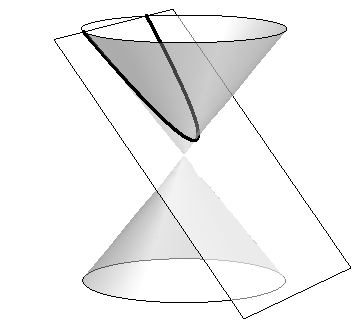
\includegraphics[scale=.25]{figures/conic_parabola}&
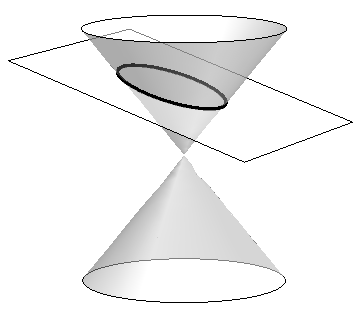
\includegraphics[scale=.25]{figures/conic_ellipse}&
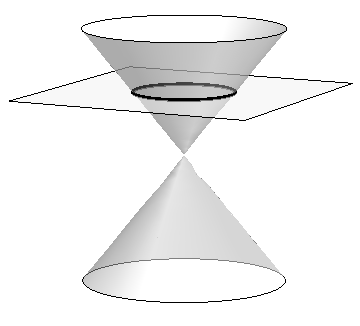
\includegraphics[scale=.25]{figures/conic_circle}&
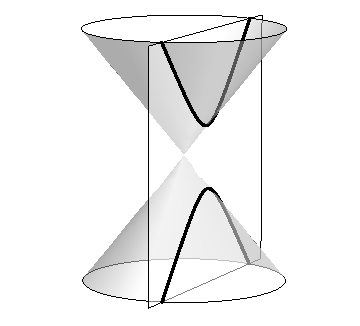
\includegraphics[scale=.25]{figures/conic_hyperbola} \\
\small Parabola &\small Ellipse & \small Circle &  \small Hyperbola
\end{tabular}
\vskip \baselineskip
\noindent%
\begin{tabular}{ccc}
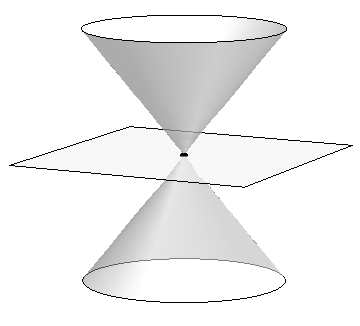
\includegraphics[scale=.25]{figures/conic_singlept}&
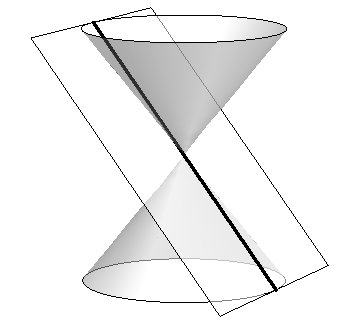
\includegraphics[scale=.25]{figures/conic_oneline}&
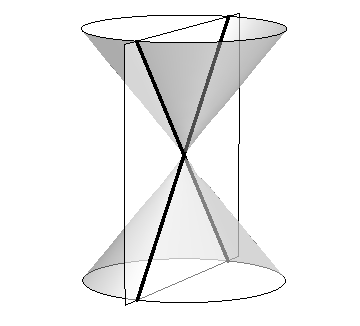
\includegraphics[scale=.25]{figures/conic_crossedlines}
\\
 \small Point& \small Line &\small  Crossed Lines 
\end{tabular}
\captionsetup{type=figure}%
\caption{Conic Sections}\label{fig:nondeg_conic}
\end{minipage}
\vskip\baselineskip

\clearpage

When the plane does contain the origin, three \textbf{degenerate} cones can be formed as shown the bottom row of  Figure \ref{fig:nondeg_conic}: a point, a line, and crossed lines. We focus here on the nondegenerate cases. \index{conic sections}\index{conic sections!degenerate}

While the above geometric constructs define the conics in an intuitive, visual way, these constructs are not very helpful when trying to analyze the shapes algebraically or consider them as the graph of a function. It can be shown that all conics can be defined by the general second--degree equation $$Ax^2+Bxy+Cy^2+Dx+Ey+F=0.$$ While this algebraic definition has its uses, most find another geometric perspective of the conics more beneficial.

Each nondegenerate conic can be defined as the \textbf{locus}, or set, of points that satisfy a certain distance property. These distance properties can be used to generate an algebraic formula, allowing us to study each conic as the graph of a function.\\

\noindent\textbf{\Large Parabolas}\\
%
%We start with a definition.
%
\definition{def:parabola}{Parabola}
{A \textbf{parabola} is the locus of all points equidistant from a point (called a \textbf{focus}) and a line (called the \textbf{directrix}) that does not contain the focus.
\index{conic sections!parabola}\index{parabola!definition}\index{directrix}\index{focus}
}

\mfigure{.5}{Illustrating the definition of the parabola and establishing an algebraic formula.}{fig:parabola_def}{figures/figparabola_def}
Figure \ref{fig:parabola_def} illustrates this definition. The point halfway between the focus and the directrix is the \textbf{vertex}. The line through the focus, perpendicular to the directrix, is the \textbf{axis of symmetry}, as the portion of the parabola on one side of this line is the mirror--image of the portion on the opposite side.

The definition leads us to an algebraic formula for the parabola. Let $P=(x,y)$ be a point on a parabola whose focus is at $F=(0,p)$ and whose directrix is at $y=-p$. (We'll assume for now that the focus lies on the $y$-axis; by placing the focus $p$ units above the $x$-axis and the directrix $p$ units below this axis, the vertex will be at $(0,0)$.)

We use the Distance Formula to find the distance $d_1$ between $F$ and $P$:
$$d_1=\sqrt{(x-0)^2+(y-p)^2}.$$
The distance $d_2$ from $P$ to the directrix is more straightforward:
$$d_2=y-(-p) = y+p.$$
These two distances are equal. Setting $d_1=d_2$, we can solve for $y$ in terms of $x$:
	\begin{align*}
	d_1&= d_2 \\
	\sqrt{x^2+(y-p)^2} &= y+p 
	\intertext{Now square both sides.}
	x^2+(y-p)^2 &= (y+p)^2 \\
	x^2+y^2-2yp+p^2 &= y^2+2yp+p^2\\
	x^2 &=4yp\\
	y&= \frac{1}{4p}x^2.
	\end{align*}
	The geometric definition of the parabola has led us to the familiar quadratic function whose graph is a parabola with vertex at the origin. When we allow the vertex to not be at $(0,0)$, we get the following standard form of the parabola.
	
	\keyidea{idea:parabola}{General Equation of a Parabola}
	{\begin{enumerate}
	\item		\textbf{Vertical Axis of Symmetry:} The equation of the parabola with vertex at $(h,k)$ and directrix $y=k-p$ in standard form is $$y=\frac{1}{4p}(x-h)^2+k.$$ The focus is at $(h,k+p)$.
	\item		\textbf{Horizontal Axis of Symmetry:} The  equation of the parabola with vertex at $(h,k)$ and directrix $x=h-p$ in standard form is $$x=\frac{1}{4p}(y-k)^2+h.$$ The focus is at $(h+p,k)$.
	\end{enumerate}
	Note: $p$ is not necessarily a positive number.
	\index{parabola!general equation}
	}
	\enlargethispage{2\baselineskip}
	
	\example{ex_conic1}{Finding the equation of a parabola}{
	Give the equation of the parabola with focus at $(1,2)$ and directrix at $y=3$.}
	{The vertex is located halfway between the focus and directrix, so $(h,k) = (1,2.5)$. This gives $p=-0.5$. Using Key Idea \ref{idea:parabola} we have the equation of the parabola as $$y=\frac{1}{4(-0.5)}(x-1)^2+2.5 = -\frac12(x-1)^2+2.5.$$
	\mfigure{.8}{The parabola described in Example \ref{ex_conic1}.}{fig:conic1}{figures/figconic1}
	The parabola is sketched in Figure \ref{fig:conic1}.
	}\\
	
	\example{ex_conic2}{Finding the focus and directrix of a parabola}{
	Find the focus and directrix of the parabola $x=\frac18y^2-y+1$. The point $(7,12)$ lies on the graph of this parabola; verify that it is equidistant from the focus and directrix.}
	{We need to put the equation of the parabola in its general form. This requires us to complete the square:
	\begin{align*}
	x &= \frac18y^2-y+1 \\
	&= \frac18\big(y^2-8y+8\big)\\
	&=	\frac18\big(y^2-8y+16 -16+8\big)\\
	&=	\frac18\big((y-4)^2 - 8\big)\\
	&=	\frac18(y-4)^2 -1.
	\end{align*}
	Hence the vertex is located at $(-1,4)$.  We have $\frac18=\frac1{4p}$, so $p=2$. We conclude that the focus is located at $(1,4)$ and the directrix is  $x=-3$. The parabola is graphed in Figure \ref{fig:conic2}, along with its focus and directrix.\\
	
\mfigure{.55}{The parabola described in Example \ref{ex_conic2}. The distances from a point on the parabola to the focus and directrix is given.}{fig:conic2}{figures/figconic2}
	
	The point $(7,12)$ lies on the graph and is $7-(-3)=10$ units from the directrix. The distance from $(7,12)$ to the focus is:
	$$\sqrt{(7-1)^2 + (12-4)^2} = \sqrt{100}=10.$$ Indeed, the point on the parabola is equidistant from the focus and directrix.
	}\\
	
	\noindent\textbf{\large Reflective Property}
	\vskip\baselineskip
	
	One of the fascinating things about the nondegenerate conic sections is their reflective properties. Parabolas have the following reflective property:
	
	\hskip 20pt \begin{minipage}[t]{.8\linewidth}
	Any ray emanating from the focus that intersects the parabola reflects off along a line perpendicular to the directrix.
	\end{minipage}\\
	\enlargethispage{\baselineskip}
	
	This is illustrated in Figure \ref{fig:conic_reflect}. The following theorem states this more rigorously.
\mfigure{.3}{Illustrating the parabola's reflective property.}{fig:conic_reflect}{figures/figconic_reflect}
	
	\theorem{thm:parabola_reflect}{Reflective Property of the Parabola}
	{Let $P$ be a point on a parabola. The tangent line to the parabola at $P$ makes equal angles with the following two lines:
		\begin{enumerate}
		\item		The line containing $P$ and the focus $F$, and
		\item		The line perpendicular to the directrix through $P$.
		\index{parabola!reflective property}
		\end{enumerate}
	}
	
	Because of this reflective property, paraboloids (the 3D analogue of parabolas) make for useful flashlight reflectors as the light from the bulb, ideally located at the focus, is reflected along parallel rays. Satellite dishes also have paraboloid shapes. Signals coming from satellites effectively approach the dish along parallel rays. The dish then \textit{focuses} these rays at the focus, where the sensor is located.\\
	
	\noindent\textbf{\Large Ellipses}
	\vskip \baselineskip
	
	\definition{def:ellipse}{Ellipse}
	{An \textbf{ellipse} is the locus of all points whose sum of distances from two fixed points, each a \textbf{focus} of the ellipse, is constant.\index{conic sections!ellipse}\index{ellipse!definition}\index{focus}
	}
	
	An easy way to visualize this construction of an ellipse is to pin both ends of a string to a board. The pins become the foci. Holding a pencil tight against the string places the pencil on the ellipse; the sum of distances from the pencil to the pins is constant: the length of the string. See Figure \ref{fig:ellipse_def}.
	\mfigure{.4}{Illustrating the construction of an ellipse with pins, pencil and string.}{fig:ellipse_def}{figures/figellipse_def}
	
	We can again find an algebraic equation for an ellipse using this geometric definition. Let the foci be located along the $x$-axis, $c$ units from the origin. Let these foci be labeled as $F_1 = (-c,0)$ and $F_2=(c,0)$. Let $P=(x,y)$ be a point on the ellipse. The sum of distances from $F_1$ to $P$ ($d_1$) and from $F_2$ to $P$ ($d_2$) is a constant $d$. That is, $d_1+d_2=d$. Using the Distance Formula, we have 
	$$\sqrt{(x+c)^2+y^2} + \sqrt{(x-c)^2+y^2} = d.$$ Using a fair amount of algebra can produce the following equation of an ellipse (note that the equation is an implicitly defined function; it has to be, as an ellipse fails the Vertical Line Test):
	$$\frac{x^2}{\left(\frac d2\right)^2} + \frac{y^2}{\left(\frac d2\right)^2-c^2} = 1.$$
	This is not particularly illuminating, but by making the substitution $a=d/2$ and $b=\sqrt{a^2-c^2}$, we can rewrite the above equation as 
	$$\frac{x^2}{a^2} + \frac{y^2}{b^2} = 1.$$ This choice of $a$ and $b$ is not without reason; as shown in Figure \ref{fig:ellipse_label}, the values of $a$ and $b$ have geometric meaning in the graph of the ellipse. 
\mfigure{.75}{Labeling the significant features of an ellipse.}{fig:ellipse_label}{figures/figellipse_label}
	
	In general, the two foci of an ellipse lie on the \textbf{major axis} of the ellipse, and the midpoint of the segment joining the two foci is the \textbf{center}. The major axis intersects the ellipse at two points, each of which is a \textbf{vertex}. The line segment through the center and perpendicular to the major axis is the \textbf{minor axis}. The ``constant sum of distances'' that defines the ellipse is the length of the major axis, i.e., $2a$.
	
	Allowing for the shifting of the ellipse gives the following standard equations.
	
	\keyidea{idea:ellipse}{Standard Equation of the Ellipse}
	{The equation of an ellipse centered at $(h,k)$ with major axis of length $2a$ and minor axis of length $2b$ in standard form is:
	\begin{enumerate}
	\item	\textbf{Horizontal major axis:} $\ds \frac{(x-h)^2}{a^2}+\frac{(y-k)^2}{b^2}=1.$
	
	\item	\textbf{Vertical major axis:} $\ds \frac{(x-h)^2}{b^2}+\frac{(y-k)^2}{a^2}=1.$
	\end{enumerate}
	The foci lie along the major axis, $c$ units from the center, where $c^2=a^2-b^2$.
	\index{ellipse!standard equation}
	}
	
	\example{ex_conic3}{Finding the equation of an ellipse}{
	Find the general equation of the ellipse graphed in Figure \ref{fig:conic3}.}
	{The center is located at $(-3,1)$. The distance from the center to a vertex is 5 units, hence $a=5$. The minor axis seems to have length 4, so $b=2$. Thus the equation of the ellipse is $$\frac{(x+3)^2}{4}+\frac{(y-1)^2}{25} = 1.$$
	\mfigure{.4}{The ellipse used in Example \ref{ex_conic3}.}{fig:conic3}{figures/figconic3}
	}\\
	
\example{ex_conic4}{Graphing an ellipse}{
Graph the ellipse defined by $4x^2+9y^2-8x-36y=-4$.}
{It is simple to graph an ellipse once it is in standard form. In order to put the given equation in standard form, we must complete the square with both the $x$ and $y$ terms. We first rewrite the equation by regrouping:
$$4x^2+9y^2-8x-36y=-4 \quad \Rightarrow \quad (4x^2-8x) + (9y^2-36y) = -4.$$
Now we complete the squares.
\begin{align*}
(4x^2-8x) + (9y^2-36y) &= -4\\
4(x^2-2x) + 9(y^2-4y) &= -4 \\
4(x^2-2x +1 - 1) + 9(y^2-4y+4-4) &= - 4\\
4\big((x-1)^2-1\big) + 9\big((y-2)^2-4\big) &= -4\\
4(x-1)^2 -4 + 9(y-2)^2-36 &= -4 \\
4(x-1)^2 + 9(y-2)^2 &= 36 \\
\frac{(x-1)^2}{9} + \frac{(y-2)^2}{4} &= 1.
\end{align*}
We see the center of the ellipse is at $(1,2)$. We have $a=3$ and $b=2$; the major axis is horizontal, so the vertices are located at $(-2,2)$ and $(4,2)$. We find $c=\sqrt{9-4} = \sqrt{5}\approx 2.24.$ The foci are located along the major axis, approximately $2.24$ units from the center, at $(1\pm 2.24,2)$. This is all graphed in Figure \ref{fig:conic4}
\mfigure{.82}{Graphing the ellipse in Example \ref{ex_conic4}.}{fig:conic4}{figures/figconic4}.
}\\

\noindent\textbf{\large Eccentricity}
\vskip\baselineskip

When $a=b$, we have a circle. The general equation becomes $$\frac{(x-h)^2}{a^2} + \frac{(y-k)^2}{a^2} = 1 \quad \Rightarrow (x-h)^2 + (y-k)^2 = a^2,$$ the familiar equation of the circle centered at $(h,k)$ with radius $a$.  Since $a=b$, $c = \sqrt{a^2-b^2}=0$. The circle has ``two'' foci, but they lie on the same point, the center of the circle. 



Consider Figure \ref{fig:ellipse_ecc}, where several ellipses are graphed with $a=1$. In (a), we have $c=0$ and the ellipse is a circle. As $c$ grows, the resulting ellipses look less and less circular. A measure of this ``noncircularness'' is \textit{eccentricity}.

\mtable{.43}{Understanding the eccentricity of an ellipse.}{fig:ellipse_ecc}{%
\begin{tabular}{c}
\myincludegraphics[scale=.75]{figures/figellipse_ecca}\\
(a)\\
\myincludegraphics[scale=.75]{figures/figellipse_eccb}\\
(b)\\
\myincludegraphics[scale=.75]{figures/figellipse_eccc}\\
(c)\\
\myincludegraphics[scale=.75]{figures/figellipse_eccd}\\
(d)
\end{tabular}
}

\definition{def:eccentricity_ellipse}{Eccentricity of an Ellipse}
{The eccentricity $e$ of an ellipse  is $\ds e=\frac{c}{a}$.
\index{ellipse!eccentricity}\index{eccentricity}
}

The eccentricity of a circle is 0; that is, a circle has no ``noncircularness.'' As $c$ approaches $a$, $e$ approaches 1, giving rise to a very noncircular ellipse, as seen in Figure \ref{fig:ellipse_ecc} (d). 

It was long assumed that planets had circular orbits. This is known to be incorrect; the orbits are elliptical. Earth has an eccentricity of $0.0167$ -- it has a nearly circular orbit.   Mercury's orbit is the most eccentric, with $e=0.2056$. (Pluto's eccentricity is greater, at $e=0.248$, the greatest of all the currently known dwarf planets.) The planet with the most circular orbit is Venus, with $e=0.0068$. The Earth's moon has an eccentricity of $e=0.0549$, also very circular.\\



\noindent \textbf{\large Reflective Property}
\vskip\baselineskip

The ellipse also possesses an interesting reflective property. Any ray emanating from one focus of an ellipse reflects off the ellipse along a line through the other focus, as illustrated in Figure \ref{fig:ellipse_reflect}. This property is given formally in the following theorem.

\mfigure{.6}{Illustrating the reflective property of an ellipse.}{fig:ellipse_reflect}{figures/figellipse_reflect}

\theorem{thm:ellipse_reflect}{Reflective Property of an Ellipse}
{Let $P$ be a point on a ellipse with foci $F_1$ and $F_2$. The tangent line to the ellipse at $P$ makes equal angles with the following two lines:\index{ellipse!reflective property}
\begin{enumerate}
	\item The line through $F_1$ and $P$, and
	\item	The line through $F_2$ and $P$. 
\end{enumerate}
}

This reflective property is useful in optics and is the basis of the phenomena experienced in whispering halls.

\vskip\baselineskip
\noindent\textbf{\Large Hyperbolas}
\vskip \baselineskip

The definition of a hyperbola is very similar to the definition of an ellipse; we essentially just change the word ``sum'' to ``difference.''

\definition{def:hyperbola}{Hyperbola}
{A \textbf{hyperbola} is the locus of all points where the absolute value of difference of distances from two fixed points, each a focus of the hyperbola, is constant.
\index{conic sections!hyperbola}\index{hyperbola!definition}\index{focus}
}

We do not have a convenient way of visualizing the construction of a hyperbola as we did for the ellipse. The geometric definition does allow us to find an algebraic expression that describes it. It will be useful to define some terms first.

The two foci lie on the \textbf{transverse axis} of the hyperbola; the midpoint of the line segment joining the foci is the \textbf{center} of the hyperbola. The transverse axis intersects the hyperbola at two points, each a \textbf{vertex} of the hyperbola. The line through the center and perpendicular to the transverse axis is the \textbf{conjugate axis.} This is illustrated in Figure \ref{fig:hyperbola_def}. It is easy to show that the constant difference of distances used in the definition of the hyperbola is the distance between the vertices, i.e., $2a$.
\mfigure{.8}{Labeling the significant features of a hyperbola.}{fig:hyperbola_def}{figures/fighyperbola_def}

\keyidea{idea:hyperbola}{Standard Equation of a Hyperbola}
{The equation of a hyperbola centered at $(h,k)$ in standard form is:
\index{hyperbola!standard equation}
\begin{enumerate}
	\item \parbox{120pt}{\textbf{Horizontal Transverse Axis:}} $\ds \frac{(x-h)^2}{a^2} - \frac{(y-k)^2}{b^2} = 1.$
	
	\item	\parbox{120pt}{\textbf{Vertical Transverse Axis:}} $\ds \frac{(y-k)^2}{a^2}-\frac{(x-h)^2}{b^2} = 1.$
\end{enumerate}
The vertices are located $a$ units from the center and the foci are located $c$ units from the center, where $c^2 = a^2+b^2$. 
}

\noindent \textbf{\large Graphing Hyperbolas}
\vskip\baselineskip

Consider the hyperbola $\frac{x^2}9-\frac{y^2}1 = 1$. Solving for $y$, we find $y=\pm\sqrt{x^2/9-1}$. As $x$ grows large, the ``$-1$'' part of the equation for $y$ becomes less significant and $y\approx \pm\sqrt{x^2/9} = \pm x/3$. That is, as $x$ gets large, the graph of the hyperbola looks very much like the lines $y=\pm x/3$. These lines are asymptotes of the hyperbola, as shown in Figure \ref{fig:hyperbola_asy1}.
\mfigure{.55}{Graphing the hyperbola $\frac{x^2}9-\frac{y^2}1 = 1$ along with its asymptotes, $y=\pm x/3$.}{fig:hyperbola_asy1}{figures/fighyperbola_asy1}

This is a valuable tool in sketching. Given the equation of a hyperbola in general form, draw a rectangle centered at $(h,k)$ with sides of length $2a$ parallel to the transverse axis and sides of length $2b$ parallel to the conjugate axis. (See Figure \ref{fig:hyperbola_asy2} for an example with a horizontal transverse axis.) The diagonals of the rectangle lie on the asymptotes. 
\mfigure{.3}{Using the asymptotes of a hyperbola as a graphing aid.}{fig:hyperbola_asy2}{figures/fighyperbola_asy2}

These lines pass through $(h,k)$.  When the transverse axis is horizontal, the slopes are $\pm b/a$; when the transverse axis is vertical, their slopes are $\pm a/b$. This gives equations:

\begin{center}
\begin{tabular}{cc}
\parbox{100pt}{\centering Horizontal \\ Transverse Axis} & \parbox{100pt}{\centering Vertical \\ Transverse Axis} \\ \ \\
$\ds y=\pm\frac ba(x-h)+k$  &$\ds  y=\pm\frac ab(x-h)+k.$
\end{tabular}
\end{center}

\example{ex_conic5}{Graphing a hyperbola}{
Sketch the hyperbola given by $\ds \frac{(y-2)^2}{25}-\frac{(x-1)^2}{4}=1.$}
{The hyperbola is centered at $(1,2)$; $a=5$ and $b=2$. In Figure \ref{fig:conic5} we draw the prescribed rectangle centered at $(1,2)$ along with the asymptotes defined by its diagonals. The hyperbola has a vertical transverse axis, so the vertices are located at $(1,7)$ and $(1,-3)$. This is enough to make a good sketch.
\mfigure{.73}{Graphing the hyperbola in Example \ref{ex_conic5}.}{fig:conic5}{figures/figconic5}

We also find the location of the foci: as $c^2= a^2+b^2$, we have $c=\sqrt{29}\approx 5.4$. Thus the foci are located at $(1,2\pm 5.4)$ as shown in the figure.
}\\

\example{ex_conic6}{Graphing a hyperbola}{
Sketch the hyperbola given by $9x^2-y^2+2y=10.$}
{We must complete the square to put the equation in general form. (We recognize this as a hyperbola since it is a general quadratic equation and the $x^2$ and $y^2$ terms have opposite signs.)

\begin{align*}
9x^2-y^2+2y &=10\\
9x^2- (y^2-2y) &= 10\\
9x^2 - (y^2-2y+1-1) &= 10\\
9x^2 -\big((y-1)^2-1\big) &= 10\\
9x^2 - (y-1)^2 &= 9\\
x^2 - \frac{(y-1)^2}{9} &=1
\end{align*}
\mfigure{.4}{Graphing the hyperbola in Example \ref{ex_conic6}.}{fig:conic6}{figures/figconic6}

We see the hyperbola is centered at $(0,1)$, with a horizontal transverse axis, where $a=1$ and $b=3$. The appropriate rectangle is sketched in Figure \ref{fig:conic6} along with the asymptotes of the hyperbola. The vertices are located at $(\pm 1,1)$. We have $c=\sqrt{10}\approx 3.2$, so the foci are located at $(\pm 3.2,1)$ as shown in the figure.
}\\
\clearpage

\noindent\textbf{\large Eccentricity}
\vskip\baselineskip

\definition{def:hyperbola_eccentricity}{Eccentricity of a Hyperbola}
{The eccentricity of a hyperbola is $\ds e=\frac ca$.\index{hyperbola!eccentricity}\index{eccentricity}
}

\mtable{.5}{Understanding the eccentricity of a hyperbola.}{fig:hyperbola_ecc}{%
\begin{tabular}{c}
\myincludegraphics{figures/fighyperbola_ecca} \\
(a)\rule[-15pt]{0pt}{25pt}\\
\myincludegraphics{figures/fighyperbola_eccb} \\
(b)\rule[-15pt]{0pt}{25pt}\\
\myincludegraphics{figures/fighyperbola_eccc} \\
(c)\rule[-15pt]{0pt}{25pt}\\
\myincludegraphics{figures/fighyperbola_eccd} \\
(d)\rule[-15pt]{0pt}{25pt}
\end{tabular}
}
Note that this is the definition of eccentricity as used for the ellipse.  When $c$ is close in value to $a$ (i.e., $e\approx 1$), the hyperbola is very narrow (looking almost like crossed lines). Figure \ref{fig:hyperbola_ecc} shows hyperbolas centered at the origin with $a=1$. The graph in (a) has $c=1.05$, giving an eccentricity of $e=1.05$, which is close to 1. As $c$ grows larger, the hyperbola widens and begins to look like parallel lines, as shown in part (d) of the figure.\\

\noindent\textbf{\large Reflective Property}
\vskip\baselineskip

Hyperbolas share a similar reflective property with ellipses. However, in the case of a hyperbola, a ray emanating from a focus that intersects the hyperbola reflects along a line containing the other focus, but moving \textit{away} from that focus. This is illustrated in Figure \ref{fig:hyperbola_reflect} (on the next page). Hyperbolic mirrors are commonly used in telescopes because of this reflective property. It is stated formally in the following theorem.

\theorem{thm:reflective_hyperbola}{Reflective Property of Hyperbolas}
{Let $P$ be a point on a hyperbola with foci $F_1$ and $F_2$. The tangent line to the hyperbola at $P$ makes equal angles with the following two lines:\index{hyperbola!reflective property}
	\begin{enumerate}
		\item The line through $F_1$ and $P$, and
		\item	The line through $F_2$ and $P$.
	\end{enumerate}
}\\

\noindent\textbf{\large Location Determination}
\vskip\baselineskip

Determining the location of a known event has many practical uses (locating the epicenter of an earthquake, an airplane crash site, the position of the person speaking in a large room, etc.).  

To determine the location of an earthquake's epicenter, seismologists use \textit{trilateration} (not to be confused with \textit{triangulation}). A seismograph allows one to determine how far away the epicenter was; using three separate readings, the location of the epicenter can be approximated.

A key to this method is knowing distances. What if this information is not available? Consider three microphones at positions $A$, $B$ and $C$ which all record a noise (a person's voice, an explosion, etc.) created at unknown location $D$. The microphone does not ``know'' when the sound was \textit{created}, only when the sound was \textit{detected}. How can the location be determined in such a situation?

\mfigure{.8}{Illustrating the reflective property of a hyperbola.}{fig:hyperbola_reflect}{figures/fighyperbola_reflect}

If each location has a clock set to the same time, hyperbolas can be used to determine the location. Suppose the microphone at position $A$ records the sound at exactly 12:00, location $B$ records the time exactly 1 second later, and location $C$ records the noise exactly 2 seconds after that. We are interested in the \textit{difference} of times. Since the speed of sound is approximately 340 m/s, we can conclude quickly that the sound was created 340 meters closer to position $A$ than position $B$. If $A$ and $B$ are a known distance apart (as shown in Figure \ref{fig:hyperbola_locate} (a)), then we can determine a hyperbola on which $D$ must lie. 

The ``difference of distances'' is 340; this is also the distance between vertices of the hyperbola. So we know $2a= 340$. Positions $A$ and $B$ lie on the foci, so $2c=1000$. From this we can find $b\approx 470$ and can sketch the hyperbola, given in part (b) of the figure. We only care about the side closest to $A$. (Why?)

We can also find the hyperbola defined by positions $B$ and $C$. In this case, $2a = 680$ as the sound traveled an extra 2 seconds to get to $C$. We still have $2c=1000$, centering this hyperbola at $(-500,500)$. We find $b\approx 367$. This hyperbola is sketched in part (c) of the figure. The intersection point of the two graphs is the location of the sound, at approximately $(188,-222.5)$.\\

\vskip 10pt
\noindent\hskip-160pt\begin{minipage}{\textwidth+150pt}
\centering
\begin{tabular}{ccccc}
\myincludegraphics{figures/fighyperbola_locate1}  &\hskip 15pt & \myincludegraphics{figures/fighyperbola_locate2} &\hskip 15pt  & \myincludegraphics{figures/fighyperbola_locate3}  \\ 
(a) & & (b) & & (c) 
\end{tabular}
\captionsetup{type=figure}
\caption{Using hyperbolas in location detection.}\label{fig:hyperbola_locate}
\end{minipage}\\

\enlargethispage{2\baselineskip}
This chapter explores curves in the plane, in particular curves that cannot be described by functions of the form $y=f(x)$. In this section, we learned of ellipses and hyperbolas that are defined implicitly, not explicitly. In the following sections, we will learn completely new ways of describing curves in the plane, using \emph{parametric equations} and \emph{polar coordinates}, then study these curves using calculus techniques.


\printexercises{exercises/09_01_exercises}
%\section{Parametric Equations}\label{sec:param_eqs}

We are familiar with sketching  shapes, such as parabolas, by following this basic procedure:

\begin{center}
\begin{tikzpicture}[>=latex]
\draw (0,0) node (A) [align=center] {Choose \\$x$} 
      (3,0) node[align=center] (B) {Use a function\\ $f$ to find $y$\\$\big(y=f(x)\big)$}
			(6.25,0) node [align=center] (C) {Plot point \\ $(x,y)$};
\draw [->](A) --(B);
\draw [->](B) -- (C);
\end{tikzpicture}
\end{center}

The \textbf{rectangular equation} $y=f(x)$ works well for some shapes like a parabola with a vertical axis of symmetry, but in the previous section we encountered several shapes that could not be sketched in this manner. (To plot an ellipse using the above procedure, we need to plot the ``top'' and ``bottom'' separately.)\index{curve!rectangular equation}

In this section we introduce a new sketching procedure:

\begin{center}
\begin{tikzpicture}[>=latex]
\draw (0,0) node (A) [align=center] {Choose \\$t$} 
      (3,1) node[align=center] (B1) {Use a function\\ $f$ to find $x$\\$\big(x=f(t)\big)$}
			(3,-1) node[align=center] (B2) {Use a function\\ $g$ to find $y$\\$\big(y=g(t)\big)$}
			(6.25,0) node [align=center] (C) {Plot point \\ $(x,y)$};
\draw [->](A) --(B1);
\draw [->](A) --(B2);
\draw [->](B1) -- (C);
\draw [->](B2) -- (C);
\end{tikzpicture}
\end{center}

Here, $x$ and $y$ are found separately but then plotted together. This leads us to a definition.

\definition{def:param_eq}{Parametric Equations and Curves}
{Let $f$ and $g$ be continuous functions on an interval $I$. The set of all points $\big(x,y\big) = \big(f(t),g(t)\big)$ in the Cartesian plane, as $t$ varies over $I$, is the \textbf{graph} of the \textbf{parametric equations} $x=f(t)$ and $y=g(t)$, where $t$ is the \textbf{parameter}. A \textbf{curve} is a graph along with the parametric equations that define it.
\index{curve!parametrically defined}\index{parametric equations!definition}
}

This is a formal definition of the word \textit{curve}. When a curve lies in a plane (such as the Cartesian plane), it is often referred to as a \textbf{plane curve}. Examples will help us understand the concepts introduced in the definition.\\

\example{ex_pareq1}{Plotting parametric functions}{ \\
Plot the graph of the parametric equations $x=t^2$, $y=t+1$ for $t$ in $[-2,2]$.}
{We plot the graphs of parametric equations in much the same manner as we plotted graphs of functions like $y=f(x)$: we make a table of values, plot points, then connect these points with a ``reasonable'' looking curve. Figure \ref{fig:pareq1}(a) shows such a table of values; note how we have 3 columns.

The points $(x,y)$ from the table are plotted in Figure \ref{fig:pareq1}(b). The points have been connected with a smooth curve. Each point has been labeled with its corresponding $t$-value. These values, along with the two arrows along the curve, are used to indicate the \textbf{orientation} of the graph. This information helps us determine the direction in which the graph is ``moving.''
%\mtable{.85}{A table of values of the parametric equations in Example \ref{ex_pareq1}.}{fig:pareq1table}{%
%\begin{tabular}{rrr}
%$t$ & $x$ & $y$ \\ \hline
%$-2$ & \phantom{$-$}4 & $-1$ \\  $-1$ & 1 & 0 \\ 0 & 0 & 1 \\ 1 & 1 & 2 \\ 2 & 4 & 3
%\end{tabular}}
%\mfigure{.65}{Sketching the graph of the parametric equations in Example \ref{ex_pareq1}.}{fig:pareq1}{figures/figpareq1}
\mtable{.75}{A table of values of the parametric equations in Example \ref{ex_pareq1} along with a sketch of their graph.}{fig:pareq1}{%
\begin{tabular}{c}
\begin{tabular}{rrr}
$t$ & $x$ & $y$ \\ \hline
$-2$ & \phantom{$-$}4 & $-1$ \\  $-1$ & 1 & 0 \\ 0 & 0 & 1 \\ 1 & 1 & 2 \\ 2 & 4 & 3
\end{tabular}\\ \\
(a)\\
\myincludegraphics{figures/figpareq1}\\
(b)
\end{tabular}}
}\\

We often use the letter $t$ as the parameter as we often regard $t$ as representing \textit{time}. Certainly there are many contexts in which the parameter is not time, but it can be helpful to think in terms of time as one makes sense of parametric plots and their orientation (for instance, ``At time $t=0$ the position is $(1,2)$ and at time $t=3$ the position is $(5,1)$.'').
\\

\example{ex_pareq2}{Plotting parametric functions}{ \\ Sketch the graph of the parametric equations $x=\cos^2t$, $y=\cos t+1$ for $t$ in $[0,\pi]$.}
{We again start by making a table of values in Figure \ref{fig:pareq2}(a), then plot the points $(x,y)$ on the Cartesian plane in Figure \ref{fig:pareq2}(b).
%\mtable{.46}{A table of values of the parametric equations in Example \ref{ex_pareq2}.}{fig:pareq2_table}{%
%\begin{tabular}{ccc}
%$t$ & $x$ & $y$ \\ \hline
%0 & 1 & 2 \\
%$\pi/4$ & $1/2$ & $1+\sqrt{2}/2$ \\
%$\pi/2$ & 0 & 1\\
%$3\pi/4$ & $1/2$ & $1-\sqrt{2}/2$ \\
%$\pi$ & 1 & 0
%\end{tabular}
%}
%\mfigure{.28}{Sketching the graph of the parametric equations in Example \ref{ex_pareq2}.}{fig:pareq2}{figures/figpareq2}
\mtable{.35}{A table of values of the parametric equations in Example \ref{ex_pareq2} along with a sketch of their graph.}{fig:pareq2}{%
\begin{tabular}{c}
\begin{tabular}{ccc}
$t$ & $x$ & $y$ \\ \hline
0 & 1 & 2 \\
$\pi/4$ & $1/2$ & $1+\sqrt{2}/2$ \\
$\pi/2$ & 0 & 1\\
$3\pi/4$ & $1/2$ & $1-\sqrt{2}/2$ \\
$\pi$ & 1 & 0
\end{tabular}\\ \\
(a)\\
\myincludegraphics{figures/figpareq2}\\
(b)
\end{tabular}
}

It is not difficult to show that the curves in Examples \ref{ex_pareq1} and \ref{ex_pareq2} are portions of the same parabola. While the \textit{parabola} is the same, the \textit{curves} are different. In Example \ref{ex_pareq1}, if we let $t$ vary over all real numbers, we'd obtain the entire parabola. In this example, letting $t$ vary over all real numbers would still produce the same graph; this portion of the parabola would be traced, and re--traced, infinitely. The orientation shown in Figure \ref{fig:pareq2} shows the orientation on $[0,\pi]$, but this orientation is reversed on $[\pi,2\pi]$.

These examples begin to illustrate the powerful nature of parametric equations. Their graphs are far more diverse than the graphs of functions produced by ``$y=f(x)$'' functions.
}\\

\noindent\textbf{Technology Note:} Most graphing utilities can graph functions given in parametric form. Often the word ``parametric'' is abbreviated as ``PAR'' or ``PARAM'' in the  options. The user usually needs to determine the graphing window (i.e, the minimum and maximum $x$- and $y$-values), along with the values of $t$ that are to be plotted. The user is often prompted to give a $t$ minimum, a $t$ maximum, and a ``$t$-step'' or ``$\Delta t$.'' Graphing utilities effectively plot parametric functions just as we've shown here: they plots lots of points. A smaller $t$-step plots more points, making for a smoother graph (but may take longer). In Figure \ref{fig:pareq1}, the $t$-step is 1; in Figure \ref{fig:pareq2}, the $t$-step is $\pi/4$.\\

One nice feature of parametric equations is that their graphs are easy to shift. While this is not too difficult in the ``$y=f(x)$'' context, the resulting function can look rather messy. (Plus, to shift to the right by two, we replace $x$ with $x-2$, which is counter--intuitive.) The following example demonstrates this.\\

\example{ex_pareq3}{Shifting the graph of parametric functions}{ Sketch the graph of the parametric equations $x=t^2+t$, $y=t^2-t$.  Find new parametric equations that shift this graph to the right 3 places and down 2.}
{The graph of the parametric equations is given in Figure \ref{fig:pareq3} (a). It is a parabola with a axis of symmetry along the line $y=x$; the vertex is at $(0,0)$. 

In order to shift the graph to the right 3 units, we need to increase the $x$-value by 3 for every point. The straightforward way to accomplish this is simply to add 3 to the function defining $x$: $x = t^2+t+3$. To shift the graph down by 2 units, we wish to decrease each $y$-value by 2, so we subtract 2 from the function defining $y$: $y = t^2-t-2$. Thus our parametric equations for the shifted graph are $x=t^2+t+3$, $y=t^2-t-2$. This is graphed in Figure \ref{fig:pareq3} (b). Notice how the vertex is now at $(3,-2)$. 
\mtable{.73}{Illustrating how to shift graphs in Example \ref{ex_pareq3}.}{fig:pareq3}{%
\begin{tabular}{cc}
\myincludegraphics{figures/figpareq3a}\\
(a) \\
\myincludegraphics{figures/figpareq3b}\\
(b)
\end{tabular}
}
}\\

Because the $x$- and $y$-values of a graph are determined independently, the graphs of parametric functions often possess features not seen on ``$y=f(x)$'' type graphs. The next example demonstrates how such graphs can arrive at the same point more than once.\\

\example{ex_pareq4}{Graphs that cross themselves}{ Plot the parametric functions $x=t^3-5t^2+3t+11$ and $y=t^2-2t+3$ and determine the $t$-values where the graph crosses itself.}
{Using the methods developed in this section, we again plot points and graph the parametric equations as shown in Figure \ref{fig:pareq4}. It appears that the graph crosses itself at the point $(2,6)$, but we'll need to analytically determine this.
\mfigure{.4}{A graph of the parametric equations from Example \ref{ex_pareq4}.}{fig:pareq4}{figures/figpareq4}

We are looking for two different values, say, $s$ and $t$, where $x(s) = x(t)$ and $y(s) = y(t)$. That is, the $x$-values are the same precisely when the $y$-values are the same. This gives us a system of 2 equations with 2 unknowns:

$$\begin{array}{c} s^3-5s^2+3s+11 = t^3-5t^2+3t+11\rule[-7pt]{0pt}{10pt}\\
								s^2-2s+3 = t^2-2t+3
	\end{array}$$

Solving this system is not trivial but involves only algebra. Using the quadratic formula, one can solve for $t$ in the second equation and find that $\ds t = 1\pm \sqrt{s^2-2s+1}$. This can be substituted into the first equation, revealing that the graph crosses itself at $t=-1$ and $t=3$. We confirm our result by computing $x(-1) = x(3)=2$ and $y(-1) = y(3) = 6$. 
}\\

\noindent\textbf{\large Converting between rectangular and parametric equations}
\vskip \baselineskip

It is sometimes useful to rewrite equations in rectangular form (i.e., $y=f(x)$) into parametric form, and vice--versa. Converting from rectangular to parametric can be very simple: given $y=f(x)$, the parametric equations $x=t$, $y=f(t)$ produce the same graph. As an example, given $y=x^2$, the parametric equations $x=t$, $y=t^2$ produce the familiar parabola. However, other parametrizations can be used. The following example demonstrates one possible alternative.\\

\example{ex_pareq5}{Converting from rectangular to parametric}{
Consider $y=x^2$. Find parametric equations $x=f(t)$, $y=g(t)$ for the parabola where $t=\frac{dy}{dx}$. That is, $t=a$ corresponds to the point on the graph whose tangent line has slope $a$.}
{We start by computing $\frac{dy}{dx}$: $y\primeskip' = 2x$. Thus we set $t=2x$. We can solve for $x$ and find $x= t/2$. Knowing that $y=x^2$, we have $y= t^2/4$. Thus parametric equations for the parabola $y=x^2$ are $$x=t/2 \quad y=t^2/4.$$
To find the point where the tangent line has a slope of $-2$, we set $t=-2$. This gives the point $(-1, 1)$. We can verify that the slope of the line tangent to the curve at this point indeed has a slope of $-2$.
}\\

We sometimes chose the parameter to accurately model physical behavior.\\

\example{ex_pareq6}{Converting from rectangular to parametric}{
An object is fired from a height of 0ft and lands 6 seconds later, 192ft away. Assuming ideal projectile motion, the height, in feet, of the object can be described by $h(x) = -x^2/64+3x$, where $x$ is the distance in feet from the initial location. (Thus $h(0) = h(192) = 0$ft.) Find parametric equations $x=f(t)$, $y=g(t)$ for the path of the projectile where $x$ is the horizontal distance the object has traveled at time $t$ (in seconds) and $y$ is the height at time $t$.
}
{Physics tells us that the horizontal motion of the projectile is linear; that is, the horizontal speed of the projectile is constant. Since the object travels 192ft in 6s, we deduce that the object is moving horizontally at a rate of 32ft/s, giving the equation $x=32t$. As $y=-x^2/64+3x$, we find $y= -16t^2+96t$. We can quickly verify that $y\primeskip''=-32$ft/s$^2$, the acceleration due to gravity, and that the projectile reaches its maximum at $t=3$, halfway along its path.

These parametric equations make certain determinations about the object's location easy: 2 seconds into the flight the object is at the point $\big(x(2),y(2)\big) = \big(64,128\big)$. That is, it has traveled horizontally 64ft and is at a height of 128ft, as shown in Figure \ref{fig:pareq6}.
\mfigure{.8}{Graphing projectile motion in Example \ref{ex_pareq6}.}{fig:pareq6}{figures/figpareq6}
}\\

It is  sometimes necessary to convert given parametric equations into rectangular form. This can be decidedly more difficult, as some ``simple'' looking parametric equations can have very ``complicated'' rectangular equations. This conversion is often referred to as ``eliminating the parameter,'' as we are looking for a relationship between $x$ and $y$ that does not involve the parameter $t$.\\

\example{ex_pareq7}{Eliminating the parameter}{
Find a rectangular equation for the curve described by $$ x= \frac{1}{t^2+1}\quad \text{and}\quad y=\frac{t^2}{t^2+1}.$$ }
{There is not a set way to eliminate a parameter. One method is to solve for $t$ in one equation and then substitute that value in the second. We use that technique here, then show a second, simpler method.

Starting with $x= 1/(t^2+1)$, solve for $t$: $ t = \pm\sqrt{1/x-1}$. Substitute this value for $t$ in the equation for $y$:
\begin{align*}
 y &= \frac{t^2}{t^2 +1} \\
		&= \frac{1/x-1}{1/x-1+1} \\
		&= \frac{1/x - 1}{1/x} \\
		&= \left(\frac1x-1\right)\cdot x \\
		&= 1-x.
\end{align*}

\mfigure{.45}{Graphing parametric and rectangular equations for a graph in Example \ref{ex_pareq7}.}{fig:pareq7}{figures/figpareq7}
Thus $y=1-x$. One may have recognized this earlier by manipulating the equation for $y$:
$$y = \frac{t^2}{t^2+1} = 1-\frac{1}{t^2+1} = 1-x.$$ This is a shortcut that is very specific to this problem; sometimes shortcuts exist and are worth looking for.

We should be careful to limit the domain of the function $y=1-x$. The parametric equations limit $x$ to values in $(0,1]$, thus to produce the same graph we should limit the domain of $y=1-x$ to the same. 

The graphs of these functions is given in Figure \ref{fig:pareq7}. The portion of the graph defined by the parametric equations is given in a thick line; the graph defined by $y=1-x$ with unrestricted domain is given in a thin line.
}\\

\example{ex_pareq8}{Eliminating the parameter}{
Eliminate the parameter in $x=4\cos t+3$, $y= 2\sin t+1$}
{We should not try to solve for $t$ in this situation as the resulting algebra/trig would be messy. Rather, we solve for $\cos t$ and $\sin t$ in each equation, respectively. This gives $$\cos t = \frac{x-3}{4} \quad \text{and}\quad \sin t=\frac{y-1}{2}.$$
The Pythagorean Theorem gives $\cos^2t+\sin^2t=1$, so:
\begin{align*}
\cos^2t+\sin^2t &=1 \\
\left(\frac{x-3}{4}\right)^2 +\left(\frac{y-1}{2}\right)^2 &=1\\
\frac{(x-3)^2}{16}+\frac{(y-1)^2}{4} &=1
\end{align*}
\mfigure{.6}{Graphing the parametric equations $x=4\cos t+3$, $y=2\sin t+1$ in Example \ref{ex_pareq8}.}{fig:pareq8}{figures/figpareq8} 
This final equation should look familiar -- it is the equation of an ellipse! Figure \ref{fig:pareq8} plots the parametric equations, demonstrating that the graph is indeed of an ellipse with a horizontal major axis and center at $(3,1)$. 
}\\

The Pythagorean Theorem can also be used to identify parametric equations for hyperbolas. We give the parametric equations for ellipses and hyperbolas in the following Key Idea.

%\keyidea{idea:par_ellipse}{Parametric Equations for Ellipses}
%{The parametric equations 
%$$ x=a\cos t+h, \quad y=b\sin t+k$$ define an ellipse with horizontal axis of length $2a$ and vertical axis of length $2b$, centered at $(h,k)$.
%\index{ellipse!parametric equations}%\\
%}
%
%\keyidea{idea:par_hyperbola}{Parametric Equations for Hyperbolas}
%{The parametric equations
%$$ x= a\tan t+h,\quad y=\pm b\sec t+k$$ define a hyperbola with vertical transverse axis centered at $(h,k)$, and 
%$$ x=\pm a\sec t+h, \quad y=b\tan t + k$$ defines a hyperbola with horizontal transverse axis. Each has asymptotes at $y=\pm b/a(x-h)+k$.
%\index{hyperbola!parametric equations}
%}

\keyidea{idea:par_ellipse_hyperbola}{Parametric Equations of Ellipses and Hyperbolas}
{\begin{itemize}
	\item The parametric equations 
$$ x=a\cos t+h, \quad y=b\sin t+k$$ define an ellipse with horizontal axis of length $2a$ and vertical axis of length $2b$, centered at $(h,k)$.
\index{ellipse!parametric equations}
	\item The parametric equations
$$ x= a\tan t+h,\quad y=\pm b\sec t+k$$ define a hyperbola with vertical transverse axis centered at $(h,k)$, and 
$$ x=\pm a\sec t+h, \quad y=b\tan t + k$$ defines a hyperbola with horizontal transverse axis. Each has asymptotes at $y=\pm b/a(x-h)+k$.
\index{hyperbola!parametric equations}
\end{itemize}
}
%%%%% End with this??
%%%%%

\noindent\textbf{\large Special Curves}
\vskip\baselineskip

Figure \ref{fig:pareq_special} gives a small  gallery of ``interesting'' and ``famous'' curves along with parametric equations that produce them. Interested readers can begin learning more about these curves through internet searches.

One might note a feature shared by two of these graphs: ``sharp corners,'' or \textbf{cusps}. We have seen graphs with cusps before and determined that such functions are not differentiable at these points. This leads us to a definition.

%\noindent
%\begin{figure}%{\linewidth}
%\centering
%\begin{tabular}{cc}
\mtable{.5}{A gallery of interesting planar curves.}{fig:pareq_special}{%
\begin{tabular}{c}
\myincludegraphics{figures/figplanecurve1} \\
\parbox{150pt}{\centering Astroid\\ $x=\cos^3 t$\\ $y=\sin^3t$}\\ \\
 \myincludegraphics{figures/figplanecurve2} \\
 \parbox{150pt}{\centering Rose Curve\\ $x=\cos(t)\sin(4t)$\\ $y=\sin(t)\sin(4t)$}\\ \\
\myincludegraphics{figures/figplanecurve3} \\
\parbox{150pt}{\centering Hypotrochoid\\ $x=2\cos(t)+5\cos(2t/3)$\\$y=2\sin(t)-5\sin(2t/3)$} \\ \\
 \myincludegraphics{figures/figplanecurve4} \\
 \parbox{150pt}{\centering Epicycloid\\ $x=4\cos(t)-\cos(4t)$\\$y=4\sin(t)-\sin(4t)$}
\end{tabular}
}
%\caption{A gallery of interesting planar curves.}\label{fig:pareq_special}
%\end{figure}

\definition{def:smooth}{Smooth}
{A curve $C$ defined by $x=f(t)$, $y=g(t)$ is \textbf{smooth} on an interval $I$ if $\fp$ and $g\primeskip'$ are continuous on $I$ and not simultaneously 0 (except possibly at the endpoints of $I$). A curve is \textbf{piecewise smooth} on $I$ if $I$ can be partitioned into subintervals where $C$ is smooth on each subinterval.
\index{curve!smooth}\index{smooth curve}\index{cusp}
}

Consider the astroid, given by $x=\cos^3t$, $y=\sin^3t$. Taking derivatives, we have:
$$x\primeskip' = -3\cos^2t\sin t\quad \text{and}\quad y\primeskip' = 3\sin^2t\cos t.$$
It is clear that each is 0 when $t=0,\ \pi/2,\ \pi,\ldots$. Thus the astroid is not smooth at these points, corresponding to the cusps seen in the figure.


We demonstrate this once more.\\

\example{ex_pareq9}{Determine where a curve is not smooth}{
Let a curve $C$ be defined by the parametric equations $x=t^3-12t+17$ and $y=t^2-4t+8$. Determine the points, if any, where it is not smooth.}
{We begin by taking derivatives. 
$$x\primeskip' = 3t^2-12,\quad y\primeskip' = 2t-4.$$
We set each equal to 0:
$$\begin{array}{l}x\primeskip' = 0 \Rightarrow 3t^2-12=0 \Rightarrow t=\pm 2\\
  y\primeskip'=0 \Rightarrow 2t-4 = 0 \Rightarrow t=2
	\end{array}
	$$
We see at $t=2$ both $x\primeskip'$ and $y\primeskip'$ are 0; thus $C$ is not smooth at $t=2$, corresponding to the point $(1,4)$. The curve is graphed in Figure \ref{fig:pareq9}, illustrating the cusp at $(1,4)$.
\mfigure{.7}{Graphing the curve in Example \ref{ex_pareq9}; note it is not smooth at $(1,4)$.}{fig:pareq9}{figures/figpareq9}
}\\

If a curve is not smooth at $t=t_0$, it means that $x\primeskip'(t_0)=y\primeskip'(t_0)=0$ as defined. This, in turn, means that rate of change of $x$ (and $y$) is 0; that is, at that instant, neither $x$ nor $y$ is changing. If the parametric equations describe the path of some object, this means the object is at rest at $t_0$. An object at rest can make a ``sharp'' change in direction, whereas moving objects tend to change direction in a ``smooth'' fashion.

One should be careful to note that a ``sharp corner'' does not have to occur when a curve is not smooth. For instance, one can verify that $x=t^3$, $y=t^6$ produce the familiar $y=x^2$ parabola. However, in this parametrization, the curve is not smooth. A particle traveling along the parabola according to the given parametric equations comes to rest at $t=0$, though no sharp point is created.\\

Our previous experience with cusps taught us that a function was not differentiable at a cusp. This can lead us to wonder about derivatives in the context of parametric equations and the application of other calculus concepts. Given a curve defined parametrically, how do we find the slopes of tangent lines? Can we determine concavity? We explore these concepts and more in the next section.



\printexercises{exercises/09_02_exercises}

%\section{Calculus and Parametric Equations}\label{sec:par_calc}

The previous section defined curves based on parametric equations. In this section we'll employ the techniques of calculus to study these curves.

We are still interested in lines tangent to points on a curve. They describe how the $y$-values are changing with respect to the $x$-values, they are useful in making approximations, and they indicate instantaneous direction of travel.

The slope of the tangent line is still $\frac{dy}{dx}$, and the Chain Rule allows us to calculate this in the context of parametric equations. If $x=f(t)$ and $y=g(t)$, the Chain Rule states that $$\frac{dy}{dt} = \frac{dy}{dx}\cdot\frac{dx}{dt}.$$
Solving for $\frac{dy}{dx}$, we get 
$$\frac{dy}{dx} = \frac{dy}{dt}\Bigg/\frac{dx}{dt} = \frac{g\primeskip'(t)}{\fp(t)},$$
provided that $\fp(t)\neq 0$. This is important so we label it a Key Idea.

\keyidea{idea:dydxpar}{Finding $\frac{dy}{dx}$ with Parametric Equations.}
{Let $x=f(t)$ and $y=g(t)$, where $f$ and $g$ are differentiable on some open interval $I$ and $\fp(t)\neq 0$ on $I$. Then \index{parametric equations!finding $\frac{dy}{dx}$}\index{derivative!parametric equations}
$$\frac{dy}{dx} = \frac{g\primeskip'(t)}{\fp(t)}.$$
}

We use this to define the tangent line.

\definition{def:tangent_par}{Tangent and Normal Lines}
{Let a curve $C$ be parametrized by $x=f(t)$ and $y=g(t)$, where $f$ and $g$ are differentiable functions on some interval $I$ containing $t=t_0$. The \textbf{tangent line} to $C$ at $t=t_0$ is the line through $\big(f(t_0),g(t_0)\big)$ with slope $m=g\primeskip'(t_0)/\fp(t_0)$, provided $\fp(t_0)\neq 0$.\\

The \textbf{normal line} to $C$ at $t=t_0$ is the line through $\big(f(t_0),g(t_0)\big)$ with slope $m=-\fp(t_0)/g\primeskip'(t_0)$, provided $g\primeskip'(t_0)\neq 0$.\index{tangent line}\index{normal line}\index{parametric equations!tangent line}\index{parametric equations!normal line}
}

The definition leaves two special cases to consider. When the tangent line is horizontal, the normal line is undefined by the above definition as $g\primeskip'(t_0)=0$. Likewise, when the normal line is horizontal, the tangent line is undefined. It seems reasonable that these lines be defined (one can draw a line tangent to the ``right side'' of a circle, for instance), so we add the following to the above definition.

	
\begin{enumerate}
	\item If the tangent line at $t=t_0$ has a slope of 0, the normal line to $C$ at $t=t_0$ is the line $x=f(t_0)$.
	\item		If the normal line at $t=t_0$ has a slope of 0, the tangent line to $C$ at $t=t_0$ is the line $x=f(t_0)$.
	\end{enumerate}
	
\example{ex_parcalc1}{Tangent and Normal Lines to Curves}{
Let $x=5t^2-6t+4$ and $y=t^2+6t-1$, and let $C$ be the curve defined by these equations.
\begin{enumerate}
	\item Find the equations of the tangent and normal lines to $C$ at $t=3$.
	\item	Find where $C$ has vertical and horizontal tangent lines.
\end{enumerate}
	}
	{\begin{enumerate}
		\item We start by computing $\fp(t) = 10t-6$ and $g\primeskip'(t) =2t+6$. Thus $$\frac{dy}{dx} = \frac{2t+6}{10t-6}.$$
		Make note of something that might seem unusual: $\frac{dy}{dx}$ is a function of $t$, not $x$. Just as points on the curve are found in terms of $t$, so are the slopes of the tangent lines.
		
		The point on $C$ at $t=3$ is $(31,26)$. The slope of the tangent line is $m=1/2$ and the slope of the normal line is $m=-2$. Thus,
		\begin{itemize}
			\item the equation of the tangent line is $\ds y=\frac12(x-31)+26$, and
			\item	the equation of the normal line is $\ds y=-2(x-31)+26$.
		\end{itemize}
		This is illustrated in Figure \ref{fig:parcalc1}.
		\mfigure{.5}{Graphing tangent and normal lines in Example \ref{ex_parcalc1}.}{fig:parcalc1}{figures/figparcalc1}
		
		\item		To find where $C$ has a horizontal tangent line, we set $\frac{dy}{dx}=0$ and solve for $t$. In this case, this amounts to setting $g\primeskip'(t)=0$ and solving for $t$ (and making sure that $\fp(t)\neq 0$). 
		$$g\primeskip'(t)=0 \quad \Rightarrow \quad 2t+6=0 \quad \Rightarrow \quad t=-3.$$
		The point on $C$ corresponding to $t=-3$ is $(67,-10)$; the tangent line at that point is horizontal (hence with equation $y=-10$).
		
		To find where $C$ has a vertical tangent line, we find where it has a horizontal normal line, and set $-\frac{\fp(t)}{g\primeskip'(t)}=0$. This amounts to setting $\fp(t)=0$ and solving for $t$ (and making sure that $g\primeskip'(t)\neq 0$). 
		$$\fp(t)=0 \quad \Rightarrow \quad 10t-6=0 \quad \Rightarrow \quad t=0.6.$$
		The point on $C$ corresponding to $t=0.6$ is $(2.2,2.96)$. The tangent line at that point is $x=2.2$.
	
		The points where the tangent lines are vertical and horizontal are indicated on the graph in Figure \ref{fig:parcalc1}.
		\end{enumerate}
		\vskip-\baselineskip
	}\\
	
	\example{ex_parcalc2}{Tangent and Normal Lines to a Circle}{
	\begin{enumerate}
		\item Find where the unit circle, defined by $x=\cos t$ and $y=\sin t$ on $[0,2\pi]$, has vertical and horizontal tangent lines. 
		\item	 Find the equation of the normal line at $t=t_0$.
		\end{enumerate}
		}
		{\begin{enumerate}
			\item We compute the derivative following Key Idea \ref{idea:dydxpar}:
			$$\frac{dy}{dx} = \frac{g\primeskip'(t)}{\fp(t)} = -\frac{\cos t}{\sin t}.$$
			The derivative is $0$ when $\cos t= 0$; that is, when $t=\pi/2,\ 3\pi/2$. These are the points $(0,1)$ and $(0,-1)$ on the circle.
			
			The normal line is horizontal (and hence, the tangent line is vertical) when $\sin t=0$; that is, when $t= 0,\ \pi,\ 2\pi$, corresponding to the points $(-1,0)$ and $(0,1)$ on the circle. These results should make intuitive sense.
			\item		The slope of the normal line at $t=t_0$ is $\ds m=\frac{\sin t_0}{\cos t_0} = \tan t_0$. This normal line goes through the point $(\cos t_0,\sin t_0)$, giving the line \begin{align*}y &=\frac{\sin t_0}{\cos t_0}(x-\cos t_0) + \sin t_0\\	
							&= (\tan t_0)x,
\end{align*}
as long as $\cos t_0\neq 0$. It is an important fact to recognize that the normal lines to a circle pass through its center, as illustrated in Figure \ref{fig:parcalc2}. Stated in another way, any line that passes through the center of a circle intersects the circle at right angles.
\mfigure{.4}{Illustrating how a circle's normal lines pass through its center.}{fig:parcalc2}{figures/figparcalc2}
		\end{enumerate}
	\vskip-1.5\baselineskip
		}\\

\clearpage

\example{ex_parcalc3}{Tangent lines when $\frac{dy}{dx}$ is not defined}
{Find the equation of the tangent line to the astroid $x=\cos^3 t$, $y=\sin^3t$ at $t=0$, shown in Figure \ref{fig:parcalc3}.
}
{We start by finding $x\primeskip'(t)$ and $y\primeskip'(t)$:
$$ x\primeskip'(t) = -3\sin t\cos^2t, \qquad y\primeskip'(t) = 3\cos t\sin^2t.$$
Note that both of these are 0 at $t=0$; the curve is not smooth at $t=0$ forming a cusp on the graph. Evaluating $\frac{dy}{dx}$ at this point returns the indeterminate form of ``0/0''. 
%$\frac{dy}{dx}$:
%$$\frac{dy}{dx} = \frac{-3\sin t\cos^2t}{3\cos t\sin^2t} = -\frac{\sin t}{\cos t},$$ as long as $\cos t\neq 0$ and $\sin t\neq 0$. When $t=0$, it is tempting to declare that $$\frac{dy}{dx} = -\frac{\sin 0}{\cos 0} = 0,$$ but this overlooks the fact that we canceled earlier with the stipulation that $\sin t\neq 0$. In fact, the graph of the curve has a cusp at $t=0$, as both $x\primeskip'=0$ and $y\primeskip'=0$. 

We can, however, examine the slopes of tangent lines near $t=0$, and take the limit as $t\to 0$. 
\begin{align*}
\lim_{t\to0} \frac{y\primeskip'(t)}{x\primeskip'(t)} &=\lim_{t\to0} \frac{3\cos t\sin^2t}{-3\sin t\cos^2t} \quad \text{\small (We can cancel as $t\neq 0$.)}\\
					&= \lim_{t\to0} -\frac{\sin t}{\cos t}\\
					&= 0.
\end{align*}
We have accomplished something significant. When the derivative $\frac{dy}{dx}$ returns an indeterminate form at $t=t_0$, we can define its value by setting it to be $\ds \lim_{t\to t_0} $$\frac{dy}{dx}$, if that limit exists. This allows us to find slopes of tangent lines at cusps, which can be very beneficial. 
\mfigure{.8}{A graph of an astroid.}{fig:parcalc3}{figures/figplanecurve1}

We found the slope of the tangent line at $t=0$ to be 0; therefore the tangent line is $y=0$, the $x$-axis. 
}\\

\noindent\textbf{\large Concavity}\\

We continue to analyze curves in the plane by considering their concavity; that is, we are interested in $\frac{d^2y}{dx^2}$, ``the second derivative of $y$ with respect to $x$.'' To find this, we need to find the derivative of $\frac{dy}{dx}$ with respect to $x$; that is,  $$\frac{d^2y}{dx^2}=\frac{d}{dx}\left[\frac{dy}{dx}\right],$$ but recall that $\frac{dy}{dx}$ is a function of $t$, not $x$, making this computation not straightforward. \index{concavity}\index{parametric equations!concavity}

To make the upcoming notation a bit simpler, let $h(t) = \frac{dy}{dx}$. We want $\frac{d}{dx}[h(t)]$; that is, we want $\frac{dh}{dx}$. We again appeal to the Chain Rule. Note:
$$\frac{dh}{dt} = \frac{dh}{dx}\cdot\frac{dx}{dt} \quad \Rightarrow \quad \frac{dh}{dx} = \frac{dh}{dt}\Bigg/\frac{dx}{dt}.$$

In words, to find $\frac{d^2y}{dx^2}$, we first take the derivative of $\frac{dy}{dx}$ \textit{with respect to $t$}, then divide by $x\primeskip'(t)$. We restate this as a Key Idea.

\keyidea{idea:second_der_par}{Finding $\frac{d^2y}{dx^2}$ with Parametric Equations}
{Let $x=f(t)$ and $y=g(t)$ be twice differentiable functions on an open interval $I$, where $\fp(t)\neq 0$ on $I$. Then 
\index{parametric equations!finding $\frac{d^2y}{dx^2}$}
$$\frac{d^2y}{dx^2}\quad = \quad\frac{d}{dt}\left[\frac{dy}{dx}\right]\Bigg/\frac{dx}{dt} \quad=\quad \frac{d}{dt}\left[\frac{dy}{dx}\right]\Bigg/\fp(t).$$ 
}

Examples will help us understand this Key Idea.\\

\example{ex_parcalc4}{Concavity of Plane Curves}{
Let $x=5t^2-6t+4$ and $y=t^2+6t-1$ as in Example \ref{ex_parcalc1}. Determine the $t$-intervals on which the graph is concave up/down.}
{Concavity is determined by the second derivative of $y$ with respect to $x$, $\frac{d^2y}{dx^2}$, so we compute that here following Key Idea \ref{idea:second_der_par}.

In Example \ref{ex_parcalc1}, we found $\ds\frac{dy}{dx} = \frac{2t+6}{10t-6}$ and $\fp(t) = 10t-6$. So:
\begin{align*}
\frac{d^2y}{dx^2} &= \frac{d}{dt}\left[\frac{2t+6}{10t-6}\right]\Bigg/(10t-6) \\
				&= -\frac{72}{(10t-6)^2}\Bigg/(10t-6)\\
				&= -\frac{72}{(10t-6)^3} \\&= -\frac{9}{(5t-3)^3}
\end{align*}
\mfigure{.5}{Graphing the parametric equations in Example \ref{ex_parcalc4} to demonstrate concavity.}{fig:parcalc4}{figures/figparcalc4}

The graph of the parametric functions is concave up when $\frac{d^2y}{dx^2} > 0$ and concave down when $\frac{d^2y}{dx^2} <0$. We determine the intervals when the second derivative is greater/less than 0 by first finding when it is 0 or undefined.

As the numerator of $\ds -\frac{9}{(5t-3)^3}$ is never 0, $\frac{d^2y}{dx^2} \neq 0$ for all $t$. It is undefined when $5t-3=0$; that is, when $t= 3/5$. Following the work established in Section \ref{sec:concavity}, we look at values of $t$ greater/less than $3/5$ on a number line:

\begin{center}\begin{tikzpicture}[>=latex]
		\draw [<->, thick] (-2.5,0) -- (2.5,0);
		\foreach \x / \y  in %
					{0/{$3/5$}}
		{\draw (\x,-.3) node[below] {\scriptsize \parbox{40pt}{\centering \y}} -- (\x,.3);}
		\draw (-1,.75) node {\scriptsize \parbox{50pt}{\centering $\ds \frac{d^2y}{dx^2}>0$ \\[5pt] c. up }};
		\draw (1,.75) node {\scriptsize \parbox{50pt}{\centering $\ds\frac{d^2y}{dx^2}<0$ \\[5pt] c. down }};
\end{tikzpicture}\end{center}

Reviewing Example \ref{ex_parcalc1}, we see that when $t=3/5=0.6$, the graph of the parametric equations has a vertical tangent line. This point is also a point of inflection for the graph, illustrated in Figure \ref{fig:parcalc4}.
}\\

\example{ex_parcalc5}{Concavity of Plane Curves}{
Find the points of inflection of the graph of the parametric equations $x=\sqrt{t}$, $y=\sin t$, for $0\leq t\leq 16$.}
{We need to compute $\frac{dy}{dx}$ and $\frac{d^2y}{dx^2}$. 
$$\frac{dy}{dx} = \frac{y\primeskip'(t)}{x\primeskip'(t)} = \frac{\cos t}{1/(2\sqrt{t})} = 2\sqrt{t}\cos t.$$
$$\frac{d^2y}{dx^2} = \frac{\frac{d}{dt}\left[\frac{dy}{dx}\right]}{x\primeskip'(t)} = \frac{\cos t/\sqrt{t}-2\sqrt{t}\sin t}{1/(2\sqrt{t})}=2\cos t-4t\sin t.$$
The points of inflection are found by setting $\frac{d^2y}{dx^2}=0$. This is not trivial, as equations that mix polynomials and trigonometric functions generally do not have ``nice'' solutions. 

In Figure \ref{fig:parcalc5}(a) we see a plot of the second derivative. It shows that it has zeros at approximately $t=0.5,\ 3.5,\ 6.5,\ 9.5,\ 12.5$ and $16$. These approximations are not very good, made only by looking at the graph. Newton's Method provides more accurate approximations. Accurate to 2 decimal places, we have:
$$t=0.65,\ 3.29,\ 6.36,\ 9.48,\ 12.61\ \text{and}\ 15.74.$$
The corresponding points have been plotted on the graph of the parametric equations in Figure \ref{fig:parcalc5}(b). Note how most occur near the $x$-axis, but not exactly on the axis. 
%\mfigure{.65}{A graph of $\frac{d^2y}{dx^2}$, showing where it is approximately 0.}{fig:parcalc5b}{figures/figparcalc5b}
%\mfigure{.4}{A graph of the parametric equations in Example \ref{ex_parcalc5} along with the points of inflection.}{fig:parcalc5}{figures/figparcalc5}
\mtable{.57}{In (a), a graph of $\frac{d^2y}{dx^2}$, showing where it is approximately 0. In (b), graph of the parametric equations in Example \ref{ex_parcalc5} along with the points of inflection.}{fig:parcalc5}{%
\begin{tabular}{c}
\myincludegraphics{figures/figparcalc5b}\\
(a)\\
\myincludegraphics{figures/figparcalc5}\\
(b)
\end{tabular}
} 
}\\

\noindent\textbf{\large Arc Length}\\

We continue our study of the features of the graphs of parametric equations by computing their arc length.

Recall in Section \ref{sec:arc_length} we found the arc length of the graph of a function, from $x=a$ to $x=b$, to be $$L = \int_a^b\sqrt{1+\left(\frac{dy}{dx}\right)^2}\ dx.$$
We can use this equation and convert it to the parametric equation context. Letting $x=f(t)$ and $y=g(t)$, we know that $\frac{dy}{dx} = g\primeskip'(t)/\fp(t)$. It will also be useful to calculate the differential of $x$: $$dx = \fp(t)dt \qquad \Rightarrow \qquad dt = \frac{1}{\fp(t)}\cdot dx.$$
Starting with the arc length formula above, consider:
\begin{align*}
L &= \int_a^b\sqrt{1+\left(\frac{dy}{dx}\right)^2}\ dx\\
		&= \int_a^b \sqrt{1+\frac{g\primeskip'(t)^2}{\fp(t)^2}}\ dx. 
		\intertext{Factor out the $\fp(t)^2$:}
		&= \int_a^b \sqrt{\fp(t)^2+g\primeskip'(t)^2}\cdot\underbrace{\frac1{\fp(t)}\ dx}_{=dt}\\
		&= \int_{t_1}^{t_2} \sqrt{\fp(t)^2+g\primeskip'(t)^2}\ dt.\\
\end{align*}
Note the new bounds (no longer ``$x$'' bounds, but ``$t$'' bounds). They are found by finding $t_1$ and $t_2$ such that $a= f(t_1)$ and $b=f(t_2)$. This formula is important, so we restate it as a theorem.

\theorem{thm:arc_length_parametric}{Arc Length of Parametric Curves}
{Let $x=f(t)$ and $y=g(t)$ be parametric equations with $\fp$ and $g\primeskip'$ continuous on $[t_1,t_2]$, on which the graph traces itself only once. The arc length of the graph, from $t=t_1$ to $t=t_2$, is
\index{parametric equations!arc length}\index{arc length}
$$L = \int_{t_1}^{t_2} \sqrt{\fp(t)^2+g\primeskip'(t)^2}\ dt.$$
}
\mnote{.4}{\textbf{Note:} Theorem \ref{thm:arc_length_parametric} makes use of differentiability on closed intervals, just as was done in Section \ref{sec:arc_length}.}

As before, these integrals are often not easy to compute. We start with a simple example, then give  another where we approximate the solution.\\

\example{ex_parcalc6}{Arc Length of a Circle}{
Find the arc length of the circle parametrized by $x=3\cos t$, $y=3\sin t$ on $[0,3\pi/2]$. 
}
{By direct application of Theorem \ref{thm:arc_length_parametric}, we have
\begin{align*}
L &= \int_0^{3\pi/2} \sqrt{(-3\sin t)^2 +(3\cos t)^2} \ dt.\\
\intertext{Apply the Pythagorean Theorem.}
	&= \int_0^{3\pi/2} 3 \ dt\\
	&= 3t\Big|_0^{3\pi/2} = 9\pi/2.
	\end{align*}
	
This should make sense; we know from geometry that the circumference of a circle with radius 3 is $6\pi$; since we are finding the arc length of $3/4$ of a circle, the arc length is $3/4\cdot 6\pi = 9\pi/2$.
}\\

\example{ex_parcalc7}{Arc Length of a Parametric Curve}{
The graph of the parametric equations $x=t(t^2-1)$, $y=t^2-1$ crosses itself as shown in Figure \ref{fig:parcalc7}, forming a ``teardrop.'' Find the arc length of the teardrop.
}
{We can see by the parametrizations of $x$ and $y$ that when $t=\pm 1$, $x=0$ and $y=0$. This means we'll integrate from $t=-1$ to $t=1$. Applying Theorem \ref{thm:arc_length_parametric}, we have
\begin{align*}
L 	&= \int_{-1}^1\sqrt{(3t^2-1)^2+(2t)^2}\ dt\\
		&=	\int_{-1}^1 \sqrt{9t^4-2t^2+1} \ dt.
\end{align*}
Unfortunately, the integrand does not have an antiderivative expressible by elementary functions. We turn to numerical integration to approximate its value. Using 4 subintervals, Simpson's Rule approximates the value of the integral as $2.65051$. Using a computer, more subintervals are easy to employ, and $n=20$ gives a value of $2.71559$. Increasing $n$ shows that this value is stable and a good approximation of the actual value.
\mfigure{.45}{A graph of the parametric equations in Example \ref{ex_parcalc7}, where the arc length of the teardrop is calculated.}{fig:parcalc7}{figures/figparcalc7}
}\\
\clearpage
%\enlargethispage{2\baselineskip}
\noindent\textbf{\large Surface Area of a Solid of Revolution}\\

Related to the formula for finding arc length is the formula for finding surface area. We can adapt the formula found in Theorem \ref{thm:surface_area} from Section \ref{sec:arc_length} in a similar way as done to produce the formula for arc length done before.

%\setboxwidth{100pt}
\theorem{thm:surface_area_parametric}{Surface Area of a Solid of Revolution}
{Consider the graph of the parametric equations $x=f(t)$ and $y=g(t)$, where $\fp$ and $g\primeskip'$ are continuous on an open interval $I$ containing $t_1$ and $t_2$ on which the graph does not cross itself.\index{surface area!solid of revolution}\index{integration!surface area}\index{parametric equations!surface area}
\begin{enumerate}
	\item	The surface area of the solid formed by revolving the graph about the $x$-axis is (where $g(t)\geq~0$ on $[t_1,t_2]$):
	$$\text{Surface Area} = 2\pi\int_{t_1}^{t_2} g(t)\sqrt{\fp(t)^2+g\primeskip'(t)^2}\ dt.$$
	
	\item	The surface area of the solid formed by revolving the graph about the $y$-axis is (where $f(t)\geq~0$ on $[t_1,t_2]$):
	$$\text{Surface Area} = 2\pi\int_{t_1}^{t_2} f(t)\sqrt{\fp(t)^2+g\primeskip'(t)^2}\ dt.$$
	\end{enumerate}
\vskip-\baselineskip
}
%\restoreboxwidth

\example{ex_parcalc8}{Surface Area of a Solid of Revolution}{
Consider the teardrop shape formed by the parametric equations $x=t(t^2-1)$, $y=t^2-1$ as seen in Example \ref{ex_parcalc7}. Find the surface area if this shape is rotated about the $x$-axis, as shown in Figure \ref{fig:parcalc8}.}
{The teardrop shape is formed between $t=-1$ and $t=1$. Using Theorem \ref{thm:surface_area_parametric}, we see we need for $g(t)\geq 0$ on $[-1,1]$, and this is not the case. To fix this, we simplify replace $g(t)$ with $-g(t)$, which flips the whole graph about the $x$-axis (and does not change the surface area of the resulting solid). The surface area is: 
\begin{align*}
\text{Area}\ S &= 2\pi\int_{-1}^1 (1-t^2)\sqrt{(3t^2-1)^2+(2t)^2}\ dt\\
		&=	2\pi\int_{-1}^1 (1-t^2)\sqrt{9t^4-2t^2+1} \ dt.
		\end{align*}
Once again we arrive at an integral that we cannot compute in terms of elementary functions. Using Simpson's Rule with $n=20$, we find the area to be $S=9.44$. Using larger values of $n$ shows this is accurate to 2 places after the decimal.
\mfigurethree{width=150pt,3Dmenu,activate=onclick,deactivate=pageinvisible,
3Droll=0,
3Dortho=0.004,
3Dc2c=0.7469545602798462 0.6216799020767212 0.23573943972587585,
3Dcoo=0 0.000 0,
3Droo=120.71813597868993,
3Dlights=Headlamp,add3Djscript=asylabels.js}{width=150pt}{.4}{Rotating a teardrop shape about the $x$-axis in Example \ref{ex_parcalc8}.}{fig:parcalc8}{figures/figparcalc8}
}\\

After defining a new way of creating curves in the plane, in this section we have applied calculus techniques to the parametric equation defining these curves to study their properties. In the next section, we define another way of forming curves in the plane. To do so, we create a new coordinate system, called \emph{polar coordinates}, that identifies points in the plane in a manner different than from measuring distances from the $y$- and $x$- axes.

\printexercises{exercises/09_03_exercises}
%\section{Introduction to Polar Coordinates}\label{sec:polar}

We are generally introduced to the idea of graphing curves by relating $x$-values to $y$-values through a function $f$. That is, we set $y=f(x)$, and plot lots of point pairs $(x,y)$ to get a good notion of how the curve looks. This method is useful but has limitations, not least of which is that curves that ``fail the vertical line test'' cannot be graphed without using multiple functions.

The previous two sections introduced and studied a new way of plotting points in the $x,y$-plane. Using parametric equations, $x$ and $y$ values are computed independently and then plotted together. This method allows us to graph an extraordinary range of curves. This section introduces yet another way to plot points in the plane: using \textbf{polar coordinates}. \\

\noindent\textbf{\large Polar Coordinates}\\

Start with a point $O$ in the plane called the \textbf{pole} (we will always identify this point with the origin). From the pole, draw a ray, called the \textbf{initial ray} (we will always draw this ray horizontally, identifying it with the positive $x$-axis). A point $P$ in the plane is determined by the distance $r$ that $P$ is from $O$, and the angle $\theta$ formed between the initial ray and the segment $\overline{OP}$ (measured counter-clockwise). We record the distance and angle as an ordered pair $(r,\theta)$. To avoid confusion with rectangular coordinates, we will denote polar coordinates with the letter $P$, as in $P(r,\theta)$. This is illustrated in Figure \ref{fig:polar_intro1}\index{polar coordinates}\index{polar!coordinates}

\mtable{.7}{Illustrating polar coordinates.}{fig:polar_intro1}{%
\begin{tikzpicture}[>=latex]
	\draw[thick,->] (0,0) node [below] {$O$} -- (3,0) node [below] {initial ray} ;
	\filldraw (0,0) circle (1.5pt);
	\filldraw [rotate=55] (2,0) circle (1.5pt);
	\draw [thick,rotate=55] (0,0)-- node [rotate=55,pos=.5,above] {$r$} (2,0) node [above] {$P=P(r,\theta)$};
	\draw [->] (.75,0) arc(0:55:.75); 
	\draw [rotate=27.5] (1,0) node {$\theta$};
\end{tikzpicture}
}

Practice will make this process more clear.\\

\example{ex_polar1}{Plotting Polar Coordinates}{
Plot the following polar coordinates:\index{polar coordinates!plotting points}
$$A = P(1,\pi/4)\quad B=P(1.5,\pi)\quad C = P(2,-\pi/3)\quad D = P(-1,\pi/4)$$
}
{%
\AddToShipoutPicture*{\put(\LenToUnit{.4\paperwidth},\LenToUnit{.04\paperheight}){%
\begin{tikzpicture}[scale=.8]
	\draw [dashed,gray] (-3.1,0) -- (0,0);
	\draw[thick,->,>=stealth] (0,0) node [below] {$O$} -- (3.5,0) ;
	\filldraw (0,0) circle (1.5pt);
	\foreach \x in {1,2,3}
	{\draw (0,0) circle (\x cm);
	\draw (\x,0) node [below right] {\x};
	}
	\foreach \x in {30,45,60,90,120,135,150}
	{\draw [rotate=\x,dashed,gray] (-3.1,0) -- (3.1,0);
	}
	%\filldraw [rotate=55] (2,0) circle (1.5pt);
	%\draw [thick,rotate=55] (0,0)-- node [rotate=55,pos=.5,above] {$r$} (2,0) node [above] {$P=P(r,\theta)$};
	%\draw [->] (.75,0) arc(0:55:.75); 
	%\draw [rotate=27.5] (1,0) node {$\theta$};
\end{tikzpicture}					
					}}
To aid in the drawing, a polar grid is provided at the bottom of this page. To place the point $A$, go out 1 unit along the initial ray (putting you on the inner circle shown on the grid), then rotate counter-clockwise $\pi/4$ radians (or $45^\circ$).  Alternately, one can consider the rotation first: think about the ray from $O$ that forms an angle of $\pi/4$ with the initial ray, then move out 1 unit along this ray (again placing you on the inner circle of the grid).

To plot $B$, go out $1.5$ units along the initial ray and rotate $\pi$ radians ($180^\circ$). 

To plot $C$, go out 2 units along the initial ray then rotate \textit{clockwise} $\pi/3$ radians, as the angle given is negative.

\mfigure{.4}{Plotting polar points in Example \ref{ex_polar1}.}{fig:polar1}{figures/figpolar1}
To plot $D$, move along the initial ray ``$-1$'' units -- in other words, ``back up'' 1 unit, then rotate counter-clockwise by $\pi/4$. The results are given in Figure \ref{fig:polar1}.
}\\

Consider the following two points: $A = P(1,\pi)$ and $B = P(-1,0)$. To locate $A$, go out 1 unit on the initial ray then rotate $\pi$ radians; to locate $B$, go out $-1$ units on the initial ray and don't rotate. One should see that $A$ and $B$ are located at the same point in the plane. We can also consider $C=P(1,3\pi)$, or $D = P(1,-\pi)$; all four of these points share the same location. 

This ability to identify a point in the plane with multiple polar coordinates is both a ``blessing'' and a ``curse.'' We will see that it is beneficial as we can plot beautiful functions that intersect themselves (much like we saw with parametric functions). The unfortunate part of this is that it can be difficult to determine when this happens. We'll explore this more later in this section.\\

\noindent\textbf{\large Polar to Rectangular Conversion}\\

It is useful to recognize both the rectangular (or, Cartesian) coordinates of a point in the plane and its polar coordinates. Figure \ref{fig:polar_intro2} shows a point $P$ in the plane with rectangular coordinates $(x,y)$ and polar coordinates $P(r,\theta)$. Using trigonometry, we can make the identities given in the following Key Idea.

\mfigure{.5}{Converting between rectangular and polar coordinates.}{fig:polar_intro2}{figures/figpolarintro2}
\keyidea{idea:polarconvert}{\parbox[t]{185pt}{Converting Between Rectangular and Polar Coordinates}}
{Given the polar point $P(r,\theta)$, the rectangular coordinates are determined by $$x=r\cos \theta\qquad y=r\sin \theta.$$

Given the rectangular coordinates $(x,y)$, the polar coordinates are determined by
$$ r^2=x^2+y^2\qquad \tan \theta = \frac yx.$$
}

\example{ex_polar2}{Converting Between Polar and Rectangular Coordinates}{
\begin{enumerate}
\item		Convert the polar coordinates $P(2,2\pi/3)$ and $P(-1,5\pi/4)$ to rectangular coordinates.
\item		Convert the rectangular coordinates $(1,2)$ and $(-1,1)$ to polar coordinates.
\end{enumerate}
}
{\begin{enumerate}
	\item \begin{enumerate}
		\item 
	We start with $P(2,2\pi/3)$. Using Key Idea \ref{idea:polarconvert}, we have 
	$$x= 2\cos (2\pi/3) = -1\qquad y = 2\sin (2\pi/3) = \sqrt{3}.$$
	So the rectangular coordinates are $(-1,\sqrt{3}) \approx (-1,1.732)$.
	
	\item The polar point $P(-1,5\pi/4)$ is converted to rectangular with:
	$$x=-1\cos (5\pi/4) = \sqrt{2}/2\qquad y= -1\sin (5\pi/4) = \sqrt{2}/2.$$
	So the rectangular coordinates are $(\sqrt{2}/2,\sqrt{2}/2) \approx (0.707,0.707)$.
	\end{enumerate}
	These points are plotted in Figure \ref{fig:polar2} (a). The rectangular coordinate system is drawn lightly under the polar coordinate system so that the relationship between the two can be seen.
	
\mtable{.6}{Plotting rectangular and polar points in Example \ref{ex_polar2}.}{fig:polar2}{%
\begin{tabular}{c}
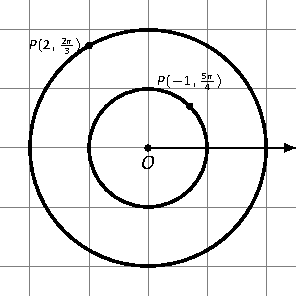
\includegraphics{figures/figpolar2}\\[5pt]
(a)\\[20pt]
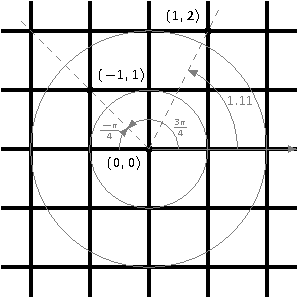
\includegraphics{figures/figpolar2b}\\[5pt]
(b)
\end{tabular}}	

\enlargethispage{2\baselineskip}
	
	\item \begin{enumerate}
		\item To convert the rectangular point $(1,2)$ to polar coordinates, we use the Key Idea to form the following two equations:
		$$1^2+2^2 = r^2 \qquad \tan \theta = \frac{2}{1}.$$
		The first equation tells us that $r=\sqrt{5}$. Using the inverse tangent function, we find
		$$\tan \theta = 2 \quad \Rightarrow \quad \theta = \tan^{-1} 2 \approx 1.11\approx 63.43^\circ.$$
		Thus polar coordinates of $(1,2)$ are $P(\sqrt{5},1.11)$.
		\item		To convert $(-1,1)$ to polar coordinates, we form the equations 
		$$(-1)^2+1^2=r^2 \qquad \tan \theta = \frac{1}{-1}.$$
		Thus $r=\sqrt{2}$. We need to be careful in computing $\theta$: using the inverse tangent function, we have $$\tan\theta = -1 \quad \Rightarrow \quad \theta = \tan^{-1}(-1) = -\pi/4 = -45^\circ.$$
		This is not the angle we desire. The range of $\tan^{-1}x $ is $(-\pi/2,\pi/2)$; that is, it returns angles that lie in the $1^\text{st}$ and $4^\text{th}$ quadrants. To find locations in the $2^\text{nd}$  and $3^\text{rd}$ quadrants, add $\pi$ to the result of $\tan^{-1}x$. So  $\pi+(-\pi/4)$ puts the angle at $3\pi/4$. Thus the polar point is $P(\sqrt{2},3\pi/4)$.
		
		An alternate method is to use the angle $\theta$ given by arctangent, but change the sign of $r$. Thus we could also refer to $(-1,1)$ as\\ $P(-\sqrt{2},-\pi/4)$.
	\end{enumerate}
These points are plotted in Figure \ref{fig:polar2} (b). The polar system is drawn lightly under the rectangular grid with rays to demonstrate the angles used.
\end{enumerate}
\vskip-\baselineskip
}\\
\clearpage

\noindent\textbf{\large Polar Functions and Polar Graphs}\\

Defining a new coordinate system allows us to create a new kind of function, a \textbf{polar function.} Rectangular coordinates lent themselves well to creating functions that related $x$ and $y$, such as $y=x^2.$ Polar coordinates allow us to create functions that relate $r$ and $\theta$. Normally these functions look like $r=f(\theta)$, although we can create functions of the form $\theta = f(r)$. The following examples introduce us to this concept.\index{polar!functions}\index{polar!functions!graphing}\\

\example{ex_polar3}{Introduction to Graphing Polar Functions}{
Describe the graphs of the following polar functions.
\begin{enumerate}
	\item $r = 1.5$
	\item $\theta = \pi/4 $
\end{enumerate}
%
%\noindent$1.\ r = 1.5 \qquad 2.\ \theta = \pi/4 $
}
{\begin{enumerate}
\item		The equation $r=1.5$ describes all points that are 1.5 units from the pole; as the angle is not specified, any $\theta$ is allowable. All points 1.5 units from the pole describes a circle of radius 1.5.

We can consider the rectangular equivalent of this equation; using $r^2=x^2+y^2$, we see that $1.5^2=x^2+y^2$, which we recognize as the equation of a circle centered at $(0,0)$ with radius 1.5. This is sketched in Figure \ref{fig:polar3}.

\item		The equation $\theta = \pi/4$ describes all points such that the line through them and the pole make an angle of $\pi/4$ with the initial ray. As the radius $r$ is not specified, it can be any value (even negative). Thus $\theta = \pi/4$ describes the line through the pole that makes an angle of $\pi/4 = 45^\circ$ with the initial ray.

We can again consider the rectangular equivalent of this equation. Combine $\tan \theta =y/x$ and $\theta =\pi/4$:
$$\tan \pi/4 = y/x \quad \Rightarrow x\tan \pi/4 = y \quad \Rightarrow y = x.$$ 
This graph is also plotted in Figure \ref{fig:polar3}.
\mfigure{.5}{Plotting standard polar plots.}{fig:polar3}{figures/figpolar3}
\end{enumerate}
\vskip-1.5\baselineskip
}\\

The basic rectangular equations of the form $x=h$ and $y=k$ create vertical and horizontal lines, respectively; the basic polar equations $r= h$ and $\theta =\alpha$ create circles and lines through the pole, respectively. With this as a foundation, we can create more complicated polar functions of the form $r=f(\theta)$. The input is an angle; the output is a length, how far in the direction of the angle to go out.

We sketch these functions much like we sketch rectangular and parametric functions: we plot lots of points and ``connect the dots'' with curves. We demonstrate this in the following example.\\

\example{ex_polar4}{Sketching Polar Functions}{ 
Sketch the polar function $r=1+\cos \theta$ on $[0,2\pi]$ by plotting points.}
{A common question when sketching curves by plotting points is ``Which points should I plot?'' With rectangular equations, we often choose ``easy'' values -- integers, then add more if needed. When plotting polar equations, start with the ``common'' angles -- multiples of $\pi/6$ and $\pi/4$. Figure \ref{fig:polar4} gives a table of just a few values of $\theta$ in $[0,\pi]$. 

Consider the point $P(2,0)$ determined by the first line of the table. The angle is 0 radians -- we do not rotate from the initial ray -- then we go out 2 units from the pole. When $\theta=\pi/6$, $r = 1.866$ (actually, it is $1+\sqrt{3}/2$); so rotate by $\pi/6$ radians and go out 1.866 units. 

The graph shown uses more points, connected with straight lines. (The points on the graph that correspond to points in the table are signified with larger dots.) Such a sketch is likely good enough to give one an idea of what the graph looks like.
}\\

\mtable{.65}{Graphing a polar function in Example \ref{ex_polar4} by plotting points.}{fig:polar4}{%
\begin{tabular}{c}
		$\begin{array}{cc}
		\theta & r=1+\cos\theta \\ \hline
 0 & 2 \\
 \pi/6 & 1.86603 \\
  \pi/2 & 1 \\
 4\pi/3 & 0.5 \\
 7 \pi /4 & 1.70711 \\
 \end{array}$ \\ \\
\myincludegraphics{figures/figpolar4}
\end{tabular}
}
\noindent\textbf{Technology Note:} Plotting functions in this way can be tedious, just as it was with rectangular functions. To obtain very accurate graphs, technology is a great aid. Most graphing calculators can plot polar functions; in the menu, set the plotting mode to something like \texttt{polar} or \texttt{POL}, depending on one's calculator. As with plotting parametric functions, the viewing ``window'' no longer determines the $x$-values that are plotted, so additional information needs to be provided. Often with the ``window'' settings are the settings for  the beginning and ending $\theta$ values (often called \texttt{$\theta_{\text{min}}$} and \texttt{$\theta_{\text{max}}$}) as well as the \texttt{$\theta_{\text{step}}$} -- that is, how far apart the $\theta$ values are spaced. The smaller the \texttt{$\theta_{\text{step}}$} value, the more accurate the graph (which also increases plotting time). Using technology, we graphed the polar function $r=1+\cos \theta$ from Example \ref{ex_polar4} in Figure \ref{fig:polar4b}.
\mfigure{.35}{Using  technology to graph a polar function.}{fig:polar4b}{figures/figpolar4b}\\

\example{ex_polar5}{Sketching Polar Functions}{
Sketch the polar function $r=\cos (2\theta)$ on $[0,2\pi]$ by plotting points.}
{We start by making a table of $\cos (2\theta)$ evaluated at common angles $\theta$, as shown in Figure \ref{fig:polar5table}. These points are then plotted in Figure \ref{fig:polar5} (a). This particular graph ``moves'' around quite a bit and one can easily forget which points should be connected to each other. To help us with this, we numbered each point in the table and on the graph. 
\clearpage

\begin{center}
\begin{minipage}[t]{125pt} \vskip0pt
$\begin{array}{ccc}
\text{Pt.} & \theta & \cos (2\theta)\\ \hline
 1 & 0 & 1. \\
 2 & \pi /6 & 0.5 \\
 3 & \pi /4 & 0. \\
 4 & \pi /3 & -0.5 \\
 5 & \pi /2 & -1. \\
 6 & 2 \pi /3 & -0.5 \\
 7 & 3 \pi /4 & 0. \\
 8 & 5 \pi /6 & 0.5 \\
 9 & \pi  & 1. \\
\end{array}$
\end{minipage}
\begin{minipage}[t]{125pt} \vskip 0pt
$\begin{array}{ccc}
\text{Pt.} & \theta & \cos (2\theta)\\ \hline
 10 & 7 \pi /6 & 0.5 \\
 11 & 5 \pi /4 & 0. \\
 12 & 4 \pi /3 & -0.5 \\
 13 & 3 \pi /2 & -1. \\
 14 & 5 \pi /3 & -0.5 \\
 15 & 7 \pi /4 & 0. \\
 16 & 11 \pi /6 & 0.5 \\
 17 & 2 \pi  & 1. \\
\end{array}$
\end{minipage}
\captionsetup{type=figure}
\caption{Tables of points for plotting a polar curve.}\label{fig:polar5table}
\end{center}
Using more points (and the aid of technology) a smoother plot can be made as shown in Figure \ref{fig:polar5} (b). This plot is an example of a \textit{rose curve}.
\mtable{.72}{Polar plots from Example \ref{ex_polar5}.}{fig:polar5}{%
\begin{tabular}{c}
\myincludegraphics{figures/figpolar5}\\[0pt]
(a) \\[0pt]
\myincludegraphics{figures/figpolar5b}\\[0pt]
(b) 
\end{tabular}
}
}\\

It is sometimes desirable to refer to a graph via a polar equation, and other times by a rectangular equation. Therefore it is necessary to be able to convert between polar and rectangular functions, which we practice in the following example. We will make frequent use of the identities found in Key Idea \ref{idea:polarconvert}.\\

\example{ex_polar6}{Converting between rectangular and polar equations.}{

\noindent
\begin{minipage}[t]{.5\linewidth}
Convert from rectangular to polar.
\begin{enumerate}
	\item $y=x^2$
	\item $xy = 1$
\end{enumerate}
\end{minipage}
\begin{minipage}[t]{.5\linewidth}
Convert from polar to rectangular.
\begin{enumerate}\addtocounter{enumi}{2}
	\item $\ds r=\frac{2}{\sin \theta-\cos\theta}$
	\item $r=2\cos \theta$
\end{enumerate}
\end{minipage}
}
{\begin{enumerate}
	\item Replace $y$ with $r\sin\theta$ and replace $x$ with $r\cos\theta$, giving:
	\begin{align*}
	y &=x^2\\
	r\sin\theta &= r^2\cos^2\theta\\
	\frac{\sin\theta}{\cos^2\theta} &= r
	\end{align*}
	We have found that $r=\sin\theta/\cos^2\theta = \tan\theta\sec\theta$. The domain of this polar function is $(-\pi/2,\pi/2)$; plot a few points to see how the familiar parabola is traced out by the polar equation.
	
	\item		We again replace $x$ and $y$ using the standard identities and work to solve for $r$:
	\begin{align*}
	xy &= 1 \\
	r\cos\theta\cdot r\sin\theta & = 1\\
	r^2 & = \frac{1}{\cos\theta\sin\theta}\\
	r & = \frac{1}{\sqrt{\cos\theta\sin\theta}}\\
	\end{align*}
	This function is valid only when the product of $\cos\theta\sin\theta$ is positive. This occurs in the first and third quadrants, meaning the domain of this polar function is $(0,\pi/2) \cup (\pi,3\pi/2)$.
	
	We can rewrite the original rectangular equation $xy=1$ as $y=1/x$. This is graphed in Figure \ref{fig:polar6}; note how it only exists in the first and third quadrants.
	\mfigure{.8}{Graphing $xy=1$ from Example \ref{ex_polar6}.}{fig:polar6}{figures/figpolar6}
		
	\item		There is no set way to convert from polar to rectangular; in general, we look to form the products $r\cos \theta$ and $r\sin\theta$, and then replace these with $x$ and $y$, respectively. We start in this problem by multiplying both sides by $\sin\theta-\cos\theta$:
	\begin{align*}
	r &= \frac{2}{\sin\theta-\cos\theta} \\
	r(\sin\theta-\cos\theta) &= 2\\
	r\sin\theta-r\cos\theta &= 2. \qquad \text{Now replace with $y$ and $x$:}\\
	y-x &= 2\\
	y &= x+2.
	\end{align*}
	The original polar equation, $r=2/(\sin\theta-\cos\theta)$ does not easily reveal that its graph is simply a line. However, our conversion shows that it is. The upcoming gallery of polar curves gives the general equations of lines in polar form.

\drawexampleline
	
	\item		By multiplying both sides by $r$, we obtain both an $r^2$ term and an $r\cos\theta$ term, which we replace with $x^2+y^2$ and $x$, respectively. 
	\begin{align*}
	r &=2\cos\theta \\
	r^2 &= 2r\cos\theta \\
	x^2+y^2 &= 2x. 
	\intertext{We recognize this as a circle; by completing the square we can find its radius and center.}
	x^2-2x+y^2 &= 0 \\
	(x-1)^2 + y^2 &=1.
	\end{align*}
	The circle is centered at $(1,0)$ and has radius 1. The upcoming gallery of polar curves gives the equations of \textit{some} circles in polar form; circles with arbitrary centers have a complicated polar equation that we do not consider here.
	\end{enumerate}
	\vskip-\baselineskip
}\\

Some curves have very simple polar equations but rather complicated rectangular ones. For instance, the equation $r=1+\cos\theta$ describes a \textit{cardioid} (a shape important to the sensitivity of microphones, among other things; one is graphed in the gallery in the Lima\c con section). It's rectangular form is not nearly as simple; it is the implicit equation
$x^4+y^4+2x^2y^2-2xy^2-2x^3-y^2=0.$ The conversion is not ``hard,'' but takes several steps, and is left as a problem in the Exercise section.\\

\noindent\textbf{\Large Gallery of Polar Curves}\\

There are a number of basic and ``classic'' polar curves, famous for their beauty and/or applicability to the sciences. \index{polar!function!gallery of graphs} This section ends with a small gallery of some of these graphs. We encourage the reader to understand how these graphs are formed, and to investigate with technology other types of polar functions.\\

\enlargethispage{2\baselineskip}
\newlength{\gallerywidth}
\setlength{\gallerywidth}{(0pt+\marginparwidth+\textwidth)/4}
\vskip \baselineskip
\noindent\hskip-\marginparwidth\hskip-25pt
\rule{25pt+\marginparwidth+\textwidth}{1pt}\\

\noindent\hskip-\marginparwidth\hskip-25pt
\textbf{\large Lines}\\

\noindent\hskip-\marginparwidth\hskip-30pt
\begin{tabular}{p{\gallerywidth}p{\gallerywidth}p{\gallerywidth}p{\gallerywidth}}
\textbf{Through the origin:} & \textbf{Horizontal line:} & \textbf{Vertical line:} & \textbf{Not through origin:} \\[5pt]
$\theta = \alpha$ & $r=a\csc\theta$ & $r=a\sec\theta$ & $\ds r=\frac{b}{\sin\theta-m\cos\theta}$ \\[10pt]
\myincludegraphics[scale=.9]{figures/figpolarline1} & \myincludegraphics[scale=.9]{figures/figpolarline2} & \myincludegraphics[scale=.9]{figures/figpolarline4} & \myincludegraphics[scale=.9]{figures/figpolarline3}
\end{tabular}

\clearpage\exercisegeometry\exerciseheader
\ \vskip0pt
\vskip-.25in
\noindent\parbox{3\gallerywidth+37pt}{\textbf{\large Circles}}\textbf{\large Spiral}\\

\noindent\hskip-5pt%
\begin{tabular}{p{\gallerywidth}p{\gallerywidth}p{\gallerywidth}p{\gallerywidth}}
\textbf{Centered on $x$-axis:} & \textbf{Centered on $y$-axis:} & \textbf{Centered on origin:} &\textbf{Archimedean spiral}\\
$r=a\cos \theta$ & $r=a\sin\theta$ & $r=a$ & $r=\theta$\\
\myincludegraphics[scale=.9]{figures/figpolarcircle1}&\myincludegraphics[scale=.9]{figures/figpolarcircle2}&\myincludegraphics[scale=.9]{figures/figpolarcircle3}&\myincludegraphics[scale=.9]{figures/figpolarspiral}
\end{tabular}\\

\noindent\textbf{\large Lima\c cons}\\
\parbox{4\gallerywidth}{Symmetric about $x$-axis: $r=a\pm b\cos\theta$; \quad Symmetric about $y$-axis:  $r=a\pm b\sin \theta$; \quad $a,b>0$}\\

\noindent\hskip-5pt%
\begin{tabular}{p{\gallerywidth}p{\gallerywidth}p{\gallerywidth}p{\gallerywidth}}
\textbf{With inner loop:} & \textbf{Cardioid:} & \textbf{Dimpled:} & \textbf{Convex:} \\[5pt]
$\ds \frac ab < 1$ & $\ds \frac ab=1$ & $\ds 1<\frac ab <2$ & $\ds \frac ab>2$ \\[10pt]
\myincludegraphics[scale=.9]{figures/figpolarlimacon1} & \myincludegraphics[scale=.9]{figures/figpolarlimacon2} & \myincludegraphics[scale=.9]{figures/figpolarlimacon3} & \myincludegraphics[scale=.9]{figures/figpolarlimacon4}
\end{tabular}\\

\noindent\textbf{\large Rose Curves}\\
\parbox{4\gallerywidth}{Symmetric about $x$-axis: $r=a \cos(n\theta)$; \quad Symmetric about $y$-axis:  $r=a\sin(n\theta)$}\\
\parbox{4\gallerywidth}{Curve contains $2n$ petals when $n$ is even and $n$ petals when $n$ is odd.}\\

\enlargethispage{20\baselineskip}
\noindent\hskip-5pt%
\begin{tabular}{p{\gallerywidth}p{\gallerywidth}p{\gallerywidth}p{\gallerywidth}}
%\textbf{With inner loop:} & \textbf{Cardioid:} & \textbf{Dimpled:} & \textbf{Convex:} \\[5pt]
$r=a\cos (2\theta)$ & $r=a\sin(2\theta)$ & $r=a\cos (3\theta)$ & $r=a\sin (3\theta)$ \\[10pt]
\myincludegraphics[scale=.9]{figures/figpolarrose1} & \myincludegraphics[scale=.9]{figures/figpolarrose2} & \myincludegraphics[scale=.9]{figures/figpolarrose4} & \myincludegraphics[scale=.9]{figures/figpolarrose3}
\end{tabular}\\
%\clearpage

\noindent%\hskip-\marginparwidth\hskip-25pt
\textbf{\large Special Curves}\\

\noindent\hskip-5pt%\hskip-\marginparwidth\hskip-30pt%
\begin{tabular}{p{\gallerywidth}p{\gallerywidth}p{\gallerywidth}p{\gallerywidth}}
\textbf{Rose curves} &  & \textbf{Lemniscate:} & \textbf{Eight Curve:} \\[5pt]
$r=a\sin (\theta/5)$ & $r=a\sin(2\theta/5)$ & $r^2=a^2\cos (2\theta)$ & $r^2=a^2\sec^4\theta\cos (2\theta)$ \\[10pt]
\myincludegraphics[scale=.9]{figures/figpolarspecial1} & \myincludegraphics[scale=.9]{figures/figpolarspecial2} & \myincludegraphics[scale=.9]{figures/figpolarspecial3} & \myincludegraphics[scale=.9]{figures/figpolarspecial4}
\end{tabular}\\

\restoregeometry
\regularheader
\clearpage

Earlier we discussed how each point in the plane does not have a unique representation in polar form. This can be a ``good'' thing, as it allows for the beautiful and interesting curves seen in the preceding gallery. However, it can also be a ``bad'' thing, as it can be difficult to determine where two curves intersect.\\

\example{ex_polar7}{Finding points of intersection with polar curves}{
Determine where the graphs of the polar equations $r=1+3\cos\theta$ and $r=\cos \theta$ intersect.
}
{As technology is generally readily available, it is usually a good idea to start with a graph. We have graphed the two functions in Figure \ref{fig:polar7}(a); to better discern the intersection points, part (b) of the figure zooms in around the origin.
\mtable{.6}{Graphs to help determine the points of intersection of the polar functions given in Example \ref{ex_polar7}.}{fig:polar7}{%
\begin{tabular}{c}
\myincludegraphics{figures/figpolar7}\\
(a)\\[10pt]
\myincludegraphics{figures/figpolar7b}\\
(b)
\end{tabular}
}
We start by setting the two functions equal to each other and solving for $\theta$:
\begin{align*}
1+3\cos\theta &= \cos \theta \\
2\cos\theta &= -1\\
\cos\theta&= -\frac12\\
\theta &= \frac{2\pi}{3}, \frac{4\pi}{3}.
\end{align*}
(There are, of course, infinite solutions to the equation $\cos\theta=-1/2$; as the lima\c con is traced out once on $[0,2\pi]$, we restrict our solutions to this interval.) 

We need to analyze this solution. When $\theta = 2\pi/3$ we obtain the point of intersection that lies in the 4$^\text{th}$ quadrant. When $\theta = 4\pi/3$, we get the point of intersection that lies in the 2$^\text{nd}$ quadrant. There is more to say about this second intersection point, however. The circle defined by $r=\cos\theta$ is traced out once on $[0,\pi]$, meaning that this point of intersection occurs while tracing out the circle a second time. It seems strange to pass by the point once and then recognize it as a point of intersection only when arriving there a ``second time.'' The first time the circle arrives at this point is when $\theta = \pi/3$.
It is key to understand that these two points are the same: $(\cos \pi/3,\pi/3)$ and $(\cos 4\pi/3,4\pi/3)$. 

To summarize what we have done so far, we have found two points of intersection: when $\theta=2\pi/3$ and when $\theta=4\pi/3$. When referencing the circle $r=\cos \theta$, the latter point is better referenced as when $\theta=\pi/3$.

There is yet another point of intersection: the pole (or, the origin). We did not recognize this intersection point using our work above as each graph arrives at the pole at a different $\theta$ value.

A graph intersects the pole when $r=0$. Considering the circle $r=\cos\theta$, $r=0$ when $\theta = \pi/2$ (and odd multiples thereof, as the circle is repeatedly traced). The lima\c con intersects the pole when $1+3\cos\theta =0$; this occurs when $\cos \theta = -1/3$, or for $\theta = \cos^{-1}(-1/3)$. This is a nonstandard angle, approximately $\theta = 1.9106 = 109.47^\circ$. The lima\c con intersects the pole twice in $[0,2\pi]$; the other angle at which the lima\c con is at the pole is the reflection of the first angle across the $x$-axis. That is, $\theta = 4.3726 = 250.53^\circ.$
}\\

If all one is concerned with is the $(x,y)$ coordinates at which the graphs intersect, much of the above work is extraneous. We know they intersect at $(0,0)$; we might not care at what $\theta$ value. Likewise, using $\theta =2\pi/3$ and $\theta=4\pi/3$ can give us the needed rectangular coordinates. However, in the next section we apply calculus concepts to polar functions. When computing the area of a region bounded by polar curves, understanding the nuances of the points of intersection becomes important.

\printexercises{exercises/09_04_exercises}

%\section{Calculus and Polar Functions} \label{sec:polarcalc}
The previous section defined polar coordinates, leading to polar functions. We investigated plotting these functions and solving a fundamental question about their graphs, namely, where do two polar graphs intersect?

We now turn our attention to answering other questions, whose solutions require the use of calculus. A basis for much of what is done in this section is the ability to turn a polar function $r=f(\theta)$ into a set of parametric equations. Using the identities $x=r\cos \theta$ and $y=r\sin \theta$, we can create the parametric equations $x=f(\theta)\cos\theta$, $y=f(\theta)\sin\theta$ and apply the concepts of Section \ref{sec:par_calc}.\\

\noindent\textbf{\large Polar Functions and $\ds \frac{dy}{dx}$}\\

We are interested in the lines tangent to a given graph, regardless of whether that graph is produced by rectangular, parametric, or polar equations. In each of these contexts, the slope of the tangent line is $\frac{dy}{dx}$. Given $r=f(\theta)$, we are generally \textit{not} concerned with $r\,'=\fp(\theta)$; that describes how fast $r$ changes with respect to $\theta$. Instead, we will use $x=f(\theta)\cos\theta$, $y=f(\theta)\sin\theta$ to compute $\frac{dy}{dx}$. 

Using Key Idea \ref{idea:dydxpar} we have $$\frac{dy}{dx} = \frac{dy}{d\theta}\Big/\frac{dx}{d\theta}.$$ Each of the two derivatives on the right hand side of the equality requires the use of the Product Rule. We state the important result as a Key Idea.\\

\keyidea{idea:dydxpol}{Finding $\frac{dy}{dx}$ with Polar Functions}
{Let $r=f(\theta)$ be a polar function. With $x=f(\theta)\cos\theta$ and $y=f(\theta)\sin\theta$,
\index{polar!functions!finding $\frac{dy}{dx}$}\index{tangent line}
$$\frac{dy}{dx} = \frac{\fp(\theta)\sin\theta+f(\theta)\cos\theta}{\fp(\theta)\cos\theta-f(\theta)\sin\theta}.$$
}

\example{ex_polcalc1}{Finding $\frac{dy}{dx}$ with polar functions.}
{Consider the lima\c con $r=1+2\sin\theta$ on $[0,2\pi]$.
\begin{enumerate}
	\item Find the equations of the tangent and normal lines to the graph at $\theta=\pi/4$.
	\item		Find where the graph has vertical and horizontal tangent lines.
\end{enumerate}
}
{\begin{enumerate}
	\item We start by computing $\frac{dy}{dx}$. With $\fp(\theta) = 2\cos\theta$, we have
	\begin{align*}
	\frac{dy}{dx} &= \frac{2\cos\theta\sin\theta + \cos\theta(1+2\sin\theta)}{2\cos^2\theta-\sin\theta(1+2\sin\theta)}\\
	&= \frac{\cos\theta(4\sin\theta+1)}{2(\cos^2\theta-\sin^2\theta)-\sin\theta}.
	\end{align*}
	When $\theta=\pi/4$, $\frac{dy}{dx}=-2\sqrt{2}-1$ (this requires a bit of simplification). In rectangular coordinates, the point on the graph at $\theta=\pi/4$ is $(1+\sqrt{2}/2,1+\sqrt{2}/2)$. Thus the rectangular equation of the line tangent to the lima\c con at $\theta=\pi/4$ is 
	$$y=(-2\sqrt{2}-1)\big(x-(1+\sqrt{2}/2)\big)+1+\sqrt{2}/2 \approx  -3.83 x+8.24.$$ The lima\c con and the tangent line are graphed in Figure \ref{fig:polcalc1}. 
	
	The normal line has the opposite--reciprocal slope as the tangent line, so its equation is 
	$$y \approx \frac{1}{3.83}x+1.26.$$
	\mfigure{.75}{The lima\c con in Example \ref{ex_polcalc1} with its tangent line at $\theta=\pi/4$ and points of vertical and horizontal tangency.}{fig:polcalc1}{figures/figpolcalc1}
	\drawexampleline
	
	\item		To find the horizontal lines of tangency, we find where $\frac{dy}{dx}=0$; thus we find where the numerator of our equation for $\frac{dy}{dx}$ is 0.
	$$\cos\theta(4\sin\theta+1)=0\quad \Rightarrow \quad \cos\theta=0 \quad \text{or}\quad 4\sin\theta+1=0.$$
	On $[0,2\pi]$, $\cos\theta=0$ when $\theta=\pi/2,\ 3\pi/2$. 

Setting $4\sin\theta+1=0$ gives $\theta=\sin^{-1}(-1/4)\approx -0.2527 = -14.48^\circ$. We want the results in $[0,2\pi]$; we also recognize there are two solutions, one in the 3$^\text{rd}$ quadrant and one in the 4$^\text{th}$. Using reference angles, we have our two solutions as $\theta =3.39$ and $6.03$ radians. The four points we obtained where the lima\c con has a horizontal tangent line are given in Figure \ref{fig:polcalc1} with black--filled dots.\\

To find the vertical lines of tangency, we set the denominator of $\frac{dy}{dx}=0$. 
\begin{align*}
2(\cos^2\theta -\sin^2\theta)-\sin\theta &= 0 .
\intertext{Convert the $\cos^2\theta$ term to $1-\sin^2\theta$:}
2(1-\sin^2\theta-\sin^2\theta)-\sin\theta &= 0\\
4\sin^2\theta + \sin\theta -2 &= 0.
\intertext{Recognize this as a quadratic in the variable $\sin\theta$. Using the quadratic formula, we have}
\sin\theta &= \frac{-1\pm\sqrt{33}}{8}.
\end{align*}
We solve $\sin\theta = \frac{-1+\sqrt{33}}8$ and $\sin\theta = \frac{-1-\sqrt{33}}8$:
\begin{align*}
\sin\theta &=\frac{-1+\sqrt{33}}8 & \sin\theta &= \frac{-1-\sqrt{33}}{8}\\
\theta &= \sin^{-1}\left(\frac{-1+\sqrt{33}}8\right) & \theta &= \sin^{-1}\left(\frac{-1-\sqrt{33}}8\right)\\
\theta &= 0.6349 & \theta &= -1.0030
\end{align*}
In each of the solutions above, we only get one of the possible two solutions as $\sin^{-1}x$ only returns solutions in $[-\pi/2,\pi/2]$, the 4$^\text{th}$ and $1^\text{st}$ quadrants. Again using reference angles, we have:
$$\sin\theta = \frac{-1+\sqrt{33}}8 \quad \Rightarrow \quad \theta = 0.6349,\ 2.5067 \text{ radians}$$
and 
$$\sin\theta = \frac{-1-\sqrt{33}}8 \quad \Rightarrow \quad \theta = 4.1446,\ 5.2802 \text{ radians.}$$
These points are also shown in Figure \ref{fig:polcalc1} with white--filled dots.
	\end{enumerate}
	\vskip-\baselineskip
}\\

When the graph of the polar function $r=f(\theta)$ intersects the pole, it means that $f(\alpha)=0$ for some angle $\alpha$. Thus the formula for $\frac{dy}{dx}$ in such instances is very simple, reducing simply to $$\frac{dy}{dx} = \tan \alpha.$$
This equation makes an interesting point. It tells us the slope of the tangent line at the pole is $\tan \alpha$; some of our previous work (see, for instance, Example \ref{ex_polar3}) shows us that the line through the pole with slope $\tan \alpha$ has polar equation $\theta=\alpha$. Thus when a polar graph touches the pole at $\theta=\alpha$, the equation of the tangent line at the pole is $\theta=\alpha$. \\

\example{ex_polcalc2}{Finding tangent lines at the pole.}{
Let $r=1+2\sin\theta$, a lima\c con. Find the equations of the lines tangent to the graph at the pole.
\mfigure{.35}{Graphing the tangent lines at the pole in Example \ref{ex_polcalc2}.}{fig:polcalc2}{figures/figpolcalc2}}
{We need to know when $r=0$. 
\begin{align*}
1+2\sin\theta &= 0\\
\sin\theta &= -1/2\\
\theta &= \frac{7\pi}{6},\ \frac{11\pi}6.
\end{align*}
Thus the equations of the tangent lines, in polar, are $\theta = 7\pi/6$ and $\theta = 11\pi/6$. In rectangular form, the tangent lines are $y=\tan(7\pi/6)x$ and $y=\tan(11\pi/6)x$. The full lima\c con can be seen in Figure \ref{fig:polcalc1}; we zoom in on the tangent lines in Figure \ref{fig:polcalc2}.
}\\

\noindent\textbf{\large Area}\\

When using rectangular coordinates, the equations $x=h$ and $y=k$ defined vertical and horizontal lines, respectively, and combinations of these lines create rectangles (hence the name ``rectangular coordinates''). It is then somewhat natural to use rectangles to approximate area as we did when learning about the definite integral.\index{polar!functions!area}

When using polar coordinates, the equations $\theta=\alpha$ and $r=c$ form lines through the origin and circles centered at the origin, respectively, and combinations of these curves form sectors of circles. It is then somewhat natural to calculate the area of regions defined by polar functions by first approximating with sectors of circles. 

Consider Figure \ref{fig:polararea} (a) where a region defined by $r=f(\theta)$ on $[\alpha,\beta]$ is given. (Note how the ``sides'' of the region are the lines $\theta=\alpha$ and $\theta=\beta$, whereas in rectangular coordinates the ``sides'' of regions were often the vertical lines $x=a$ and $x=b$.)
\mnote{.8}{\textbf{Note:} Recall that the area of a sector of a circle with radius $r$ subtended by an angle $\theta$ is $A = \frac12\theta r^2$.

\hfill
\begin{tikzpicture}[x=30pt,y=30pt,thick]
			\draw (2,0) arc (0:50:2) -- (0,0);
			\draw [] (0,0) -- (2,0) node [pos=.5,below] {$r$};
			\draw [fill=black] (0,0) circle (1pt);
			%\draw (1.95,1.0) node {$s$};
			\draw (0,0) node [shift={(15pt,8pt)}] {$\theta$};
			\end{tikzpicture}
\hfill\null
}

Partition the interval $[\alpha,\beta]$ into $n$ equally spaced subintervals as $\alpha = \theta_1 < \theta_2 <\cdots <\theta_{n+1}=\beta$. The length of each subinterval is $\Delta\theta = (\beta-\alpha)/n$, representing a small change in angle. The area of the region defined by the $i\,^\text{th}$ subinterval $[\theta_i,\theta_{i+1}]$ can be approximated with a sector of a circle with radius $f(c_i)$, for some $c_i$ in $[\theta_i,\theta_{i+1}]$. The area of this sector is $\frac12f(c_i)^2\Delta\theta$. This is shown in part (b) of the figure, where $[\alpha,\beta]$ has been divided into 4 subintervals. We approximate the area of the whole region by summing the areas of all sectors:
$$\text{Area} \approx \sum_{i=1}^n \frac12f(c_i)^2\Delta\theta.$$
This is a Riemann sum. By taking the limit of the sum as $n\to\infty$, we find the exact area of the region in the form of a definite integral.
\mtable{.5}{Computing the area of a polar region.}{fig:polararea}{%
\begin{tabular}{c}
\myincludegraphics{figures/figpolarea1}\\
(a)\\[10pt]
\myincludegraphics{figures/figpolarea2}\\
(b)
\end{tabular}
}
\enlargethispage{2\baselineskip}
%\clearpage

\theorem{thm:polar_area}{Area of a Polar Region}
{Let $f$ be continuous and non-negative on $[\alpha,\beta]$, where $0\leq \beta-\alpha\leq 2\pi$. The area  $A$ of the region bounded by the curve $r=f(\theta)$ and the lines $\theta=\alpha$ and $\theta=\beta$ is 
$$
A \ =\  \frac12\int_\alpha^\beta f(\theta)^2 \ d\theta\  =\  \frac12\int_\alpha^\beta r^{\,2} \ d\theta$$
}

The theorem states that $0\leq \beta-\alpha\leq 2\pi$. This ensures that region does not overlap itself, which would give a result that does not correspond directly to the area.\\

\example{ex_polcalc3}{Area of a polar region}{
Find the area of the circle defined by $r=\cos \theta$. (Recall this circle has radius $1/2$.)}
{This is a direct application of Theorem \ref{thm:polar_area}. The circle is traced out on $[0,\pi]$, leading to the integral
\begin{align*}
\text{Area} &= \frac12\int_0^\pi \cos^2\theta\ d  \theta \\
						&= \frac12\int_0^\pi \frac{1+\cos(2\theta)}{2}\ d\theta\\
						&= \frac14\big(\theta +\frac12\sin(2\theta)\big)\Bigg|_0^\pi\\
						&= \frac14\pi.
\end{align*}
Of course, we already knew the area of a circle with radius $1/2$. We did this example to demonstrate that the area formula is correct.
}\\

\mnote{.7}{\textbf{Note:} Example \ref{ex_polcalc3} requires the use of the integral $\ds\int \cos^2\theta\ d\theta$. This is handled well by using the power reducing formula as found in the back of this text. Due to the nature of the area formula, integrating $\cos^2\theta$ and $\sin^2\theta$ is required often. We offer here these indefinite integrals as a time--saving measure.\\
$$\int\cos^2\theta\ d\theta = \frac12\theta+\frac14\sin(2\theta)+C$$
$$\int\sin^2\theta\ d\theta = \frac12\theta-\frac14\sin(2\theta)+C$$
}

\example{ex_polcalc4}{Area of a polar region}{
Find the area of the cardioid $r=1+\cos\theta$ bound between $\theta=\pi/6$ and $\theta=\pi/3$, as shown in Figure \ref{fig:polcalc4}.
\mfigure{.3}{Finding the area of the shaded region of a cardioid in Example \ref{ex_polcalc4}.}{fig:polcalc4}{figures/figpolcalc4}
}
{This is again a direct application of Theorem \ref{thm:polar_area}. 
\begin{align*}
\text{Area} &= \frac12\int_{\pi/6}^{\pi/3} (1+\cos\theta)^2\ d\theta\\
				&= \frac12\int_{\pi/6}^{\pi/3} (1+2\cos\theta+\cos^2\theta)\ d\theta\\
				&= \frac12\left(\theta+2\sin\theta+\frac12\theta+\frac14\sin(2\theta)\right)\Bigg|_{\pi/6}^{\pi/3} \\
				&= \frac18\big(\pi+4\sqrt{3}-4\big) \approx 0.7587.
				\end{align*}
\vskip-\baselineskip
}\\

\noindent\textbf{Area Between Curves}\\

Our study of area in the context of rectangular functions led naturally to finding area bounded between curves. We consider the same in the context of polar functions. \index{polar!functions!area between curves}

Consider the shaded region shown in Figure \ref{fig:polarea3}. We can find the area of this region by computing the area bounded by $r_2=f_2(\theta)$ and subtracting the area bounded by $r_1=f_1(\theta)$ on $[\alpha,\beta]$. Thus
$$\text{Area}\ = \ \frac12\int_\alpha^\beta r_2^{\,2}\ d\theta - \frac12\int_\alpha^\beta r_1^{\,2}\ d\theta = \frac12\int_\alpha^\beta \big(r_2^{\,2}-r_1^{\,2}\big)\ d\theta.$$
\mfigure{.6}{Illustrating area bound between two polar curves.}{fig:polarea3}{figures/figpolarea3}

\keyidea{idea:area_between_polar}{Area Between Polar Curves}
{The area $A$ of the region bounded by $r_1=f_1(\theta)$ and $r_2=f_2(\theta)$, $\theta=\alpha$ and $\theta=\beta$, where $f_1(\theta)\leq f_2(\theta)$ on $[\alpha,\beta]$, is
$$A = \frac12\int_\alpha^\beta \big(r_2^{\,2}-r_1^{\,2}\big)\ d\theta.$$
}

\enlargethispage{2\baselineskip}
\example{ex_polcalc5}{Area between polar curves}{
Find the area bounded between the curves $r=1+\cos \theta$ and $r=3\cos\theta$, as shown in Figure \ref{fig:polcalc5}.
\mfigure{.3}{Finding the area between polar curves in Example \ref{ex_polcalc5}.}{fig:polcalc5}{figures/figpolcalc5}
}
{We need to find the points of intersection between these two functions. Setting them equal to each other, we find:
\begin{align*}
1+\cos\theta &= 3\cos \theta \\
 \cos\theta &=1/2\\
\theta &= \pm \pi/3
\end{align*}
Thus we integrate $\frac12\big((3\cos\theta)^2-(1+\cos\theta)^2\big)$ on $[-\pi/3,\pi/3]$.
\begin{align*}
\text{Area} &= \frac12\int_{-\pi/3}^{\pi/3} \big((3\cos\theta)^2-(1+\cos\theta)^2\big)\ d\theta\\
		&= \frac12\int_{-\pi/3}^{\pi/3} \big( 8\cos^2\theta-2\cos\theta-1\big)\ d\theta \\
		&= \frac12\big(2\sin(2\theta) - 2\sin\theta+3\theta\big)\Bigg|_{-\pi/3}^{\pi/3}\\
		&= \pi.
\end{align*}
Amazingly enough, the area between these curves has a ``nice'' value.
}\\

\example{ex_polcalc6}{Area defined by polar curves}{
Find the area bounded between the polar curves $r=1$ and $r=2\cos(2\theta)$, as shown in Figure \ref{fig:polcalc6} (a).}
{We need to find the point of intersection between the two curves. Setting the two functions equal to each other, we have
$$2\cos(2\theta) = 1 \quad \Rightarrow \quad \cos(2\theta) = \frac12 \quad \Rightarrow \quad 2\theta = \pi/3\quad \Rightarrow \quad \theta=\pi/6.$$
\mtable{.4}{Graphing the region bounded by the functions in Example \ref{ex_polcalc6}.}{fig:polcalc6}{%
\begin{tabular}{c}
\myincludegraphics{figures/figpolcalc6}\\
(a)\\[10pt]
\myincludegraphics{figures/figpolcalc6a}\\
(b)\\
\end{tabular}
}
In part (b) of the figure, we zoom in on the region and note that it is not really bounded \textit{between} two polar curves, but rather \textit{by} two polar curves, along with $\theta=0$. The dashed line breaks the region into its component parts. Below the dashed line, the region is defined by $r=1$, $\theta=0$ and $\theta = \pi/6$. (Note: the dashed line lies on the line $\theta=\pi/6$.) Above the dashed line the region is bounded by $r=2\cos(2\theta)$ and $\theta =\pi/6$. Since we have two separate regions, we find the area using two separate integrals.

Call the area below the dashed line $A_1$ and the area above the dashed line $A_2$. They are determined by the following integrals:
$$A_1 = \frac12\int_0^{\pi/6} (1)^2\ d\theta\qquad  A_2 = \frac12\int_{\pi/6}^{\pi/4} \big(2\cos(2\theta)\big)^2\ d\theta.$$
(The upper bound of the integral computing $A_2$ is $\pi/4$ as $r=2\cos(2\theta)$ is at the pole when $\theta=\pi/4$.)

We omit the integration details and let the reader verify that $A_1 = \pi/12$ and $A_2 = \pi/12-\sqrt{3}/8$; the total area is $A = \pi/6-\sqrt{3}/8$.
}\\

\noindent\textbf{\large Arc Length}\\

As we have already considered the arc length of curves defined by rectangular and parametric equations, we now consider it in the context of polar equations. Recall that the arc length $L$ of the graph defined by the parametric equations $x=f(t)$, $y=g(t)$ on $[a,b]$ is
\index{arc length}\index{polar!function!arc length}
\begin{equation}L = \int_a^b \sqrt{\fp(t)^2 + g\primeskip'(t)^2}\ dt = \int_a^b \sqrt{x\primeskip'(t)^2+y\primeskip'(t)^2}\ dt.\label{eq:polar_arclength}\end{equation}

Now consider the polar function $r=f(\theta)$. We again use the identities $x=f(\theta)\cos\theta$ and $y=f(\theta)\sin\theta$ to create parametric equations based on the polar function. We compute $x\primeskip'(\theta)$ and $y\primeskip'(\theta)$ as done before when computing $\frac{dy}{dx}$, then apply Equation \eqref{eq:polar_arclength}.

The expression $x\primeskip'(\theta)^2+y\primeskip'(\theta)^2$ can be simplified a great deal; we leave this as an exercise and state that $$x\primeskip'(\theta)^2+y\primeskip'(\theta)^2 = \fp(\theta)^2+f(\theta)^2.$$ This leads us to the  arc length formula.

\keyidea{idea:polar_arclength}{Arc Length of Polar Curves}
{Let  $r=f(\theta)$ be a polar function with $\fp$ continuous on an open interval $I$ containing $[\alpha,\beta]$, on which the graph traces itself only once. The arc length $L$ of the graph on $[\alpha,\beta]$ is
$$L = \int_\alpha^\beta \sqrt{\fp(\theta)^2+f(\theta)^2}\ d\theta = \int_\alpha^\beta\sqrt{(r\,')^2+ r^2}\ d\theta.$$
}

\example{ex_polcalc7}{Arc length of a lima\c con}{
Find the arc length of the lima\c con $r=1+2\sin t$.}
{With $r=1+2\sin t$, we have $r\,' = 2\cos t$. The lima\c con is traced out once on $[0,2\pi]$, giving us our bounds of integration. Applying Key Idea \ref{idea:polar_arclength}, we have
\begin{align*}
L 	&= \int_0^{2\pi} \sqrt{(2\cos\theta)^2+(1+2\sin\theta)^2}\ d\theta \\
		&=	\int_0^{2\pi} \sqrt{4\cos^2\theta+4\sin^2\theta +4\sin\theta+1}\ d\theta\\
		&=	\int_0^{2\pi} \sqrt{4\sin\theta+5}\ d\theta\\
		&\approx 13.3649.
\end{align*}
\mfigure{.8}{The lima\c con in Example \ref{ex_polcalc7} whose arc length is measured.}{fig:polcalc7}{figures/figpolcalc7}
The final integral cannot be solved in terms of elementary functions, so we resorted to a numerical approximation. (Simpson's Rule, with $n=4$, approximates the value with $13.0608$. Using $n=22$ gives the value above, which is accurate to 4 places after the decimal.) 
}\\

\noindent\textbf{\large Surface Area}\\

The formula for arc length leads us to a formula for surface area. The following Key Idea is based on Key Idea \ref{idea:surface_area_parametric}.

\keyidea{idea:surface_area_polar}{Surface Area of a Solid of Revolution}
{Consider the graph of the polar equation $r=f(\theta)$, where $\fp$ is continuous on an open interval containing $[\alpha,\beta]$ on which the graph does not cross itself.
\index{surface area!solid of revolution}\index{polar!function!surface area}\index{integration!surface area}
	\begin{enumerate}
		\item The surface area of the solid formed by revolving the graph about the initial ray ($\theta=0$) is:
		$$\text{Surface Area} = 2\pi\int_\alpha^\beta f(\theta)\sin\theta\sqrt{\fp(\theta)^2+f(\theta)^2}\ d\theta.$$
		\item The surface area of the solid formed by revolving the graph about the line $\theta=\pi/2$ is:
		$$\text{Surface Area} = 2\pi\int_\alpha^\beta f(\theta)\cos\theta\sqrt{\fp(\theta)^2+f(\theta)^2}\ d\theta.$$
	\end{enumerate}
}
\clearpage

\example{ex_polcalc8}{Surface area determined by a polar curve}{
Find the surface area formed by revolving one petal of the rose curve $r=\cos(2\theta)$ about its central axis (see Figure \ref{fig:polcalc8}).}
{\mtable{.7}{Finding the surface area of a rose--curve petal that is revolved around its central axis.}{fig:polcalc8}{%
\begin{tabular}{c}
\myincludegraphics{figures/figpolcalc8}\\
(a)\\[10pt]
%%\ifthenelse{\boolean{in_threeD}}{{%
%%\myincludegraphicsthree[width=150pt,3Dmenu,activate=onclick,deactivate=pageinvisible,
%%3Droll=0,
%%3Dortho=0.009,
%%3Dc2c=0.41893383860588074 -0.887881875038147 0.1901581883430481,
%%3Dcoo=65.85308837890625 6.341495513916016 17.98039436340332,
%%3Droo=85,
%%3Dlights=Headlamp,add3Djscript=asylabels.js]{figures/figpolcalc8a_3D}}}%
%%{\myincludegraphics[scale=1.25,trim=5mm 5mm 5mm 5mm,clip=true]{figures/figpolcalc8a}}\\
%%%\myincludegraphicsthree{width=150pt,3Dmenu,activate=onclick,deactivate=pageinvisible,
%%%3Droll=0,
%%%3Dortho=0.009,
%%%3Dc2c=0.41893383860588074 -0.887881875038147 0.1901581883430481,
%%%3Dcoo=65.85308837890625 6.341495513916016 17.98039436340332,
%%%3Droo=85,
%%%3Dlights=Headlamp,add3Djscript=asylabels.js}{scale=1.25,trim=5mm 5mm 5mm 5mm,clip=true}{figures/figpolcalc8a}\\
%%\myincludegraphics[scale=1.25,trim=5mm 5mm 5mm 5mm,clip=true]{figures/figpolcalc8a}\\
\myincludegraphicsthree{width=150pt,3Dmenu,activate=onclick,deactivate=pageinvisible,
3Droll=0,
3Dortho=0.009,
3Dc2c=0.41893383860588074 -0.887881875038147 0.1901581883430481,
3Dcoo=65.85308837890625 6.341495513916016 17.98039436340332,
3Droo=85,
3Dlights=Headlamp,add3Djscript=asylabels.js}{scale=1.0,trim=0mm 0mm 0mm 0mm,clip=true}{figures/figpolcalc8a}\\
(b)\\
\end{tabular}
}
We choose, as implied by the figure, to revolve the portion of the curve that lies on $[0,\pi/4]$ about the initial ray. Using Key Idea \ref{idea:surface_area_polar} and the fact that $\fp(\theta) = -2\sin(2\theta)$, we have
\begin{align*}
\text{Surface Area} &= 2\pi\int_0^{\pi/4} \cos(2\theta)\sin(\theta)\sqrt{\big(-2\sin(2\theta)\big)^2+\big(\cos(2\theta)\big)^2}\ d\theta \\
&\approx 1.36707.
\end{align*}
The integral is another that cannot be evaluated in terms of elementary functions. Simpson's Rule, with $n=4$, approximates the value at $1.36751$.%; with $n=10$, the value is accurate to 4 decimal places.
}\\


This chapter has been about curves in the plane. While there is great mathematics to be discovered in the two dimensions of a plane, we live in a three dimensional world and hence we should also look to do mathematics in 3D -- that is, in \emph{space}. The next chapter begins our exploration into space by introducing the topic of \emph{vectors}, which are incredibly useful and powerful mathematical objects.
\printexercises{exercises/09_05_exercises}
%
%
%%
%%
%%%
%%%%
%%%\addtocounter{chapter}{9}
%\clearpage{\pagestyle{empty}\cleardoublepage}
%\chapter{Vectors}
%\thispagestyle{empty}
%This chapter introduces a new mathematical object, the \sword{vector}. Defined in Section \ref{sec:vector_intro}, we will see that vectors provide a powerful language for describing quantities that have magnitude and direction aspects. A simple example of such a quantity is force: when applying a force, one is generally interested in how much force is applied (i.e., the magnitude of the force) and the direction in which the force was applied. Vectors will play an important role in many of the subsequent chapters in this text. 

This chapter begins with moving our mathematics out of the plane and into ``space.'' That is, we begin to think mathematically not only in two dimensions, but in three. With this foundation, we can explore vectors both in the plane and in space. 

\section{Introduction to Cartesian Coordinates in Space}\label{sec:space_coord}

Up to this point in this text we have considered mathematics in a 2--dimensional world. We have plotted graphs on the $x$-$y$ plane using rectangular and polar coordinates and found the area of regions in the plane. We have considered properties of \textit{solid} objects, such as volume and surface area, but only by first defining a curve in the plane and then rotating it out of the plane.

While there is wonderful mathematics to explore in ``2D,'' we live in a ``3D'' world and eventually we will want to apply mathematics involving this third dimension. In this section we introduce Cartesian coordinates in space and explore basic surfaces. This will lay a foundation for much of what we do in the remainder of the text.\\

Each point $P$ in space can be represented with an ordered triple, $P=(a,b,c)$, where $a$, $b$ and $c$ represent the relative position of $P$ along the $x$-, $y$- and $z$-axes, respectively. Each axis is perpendicular to the other two.

Visualizing points in space on paper can be problematic, as we are trying to represent a 3-dimensional concept on a 2--dimensional medium. We cannot draw three lines representing the three axes in which each line is perpendicular to the other two. Despite this issue, standard conventions exist for plotting shapes in space that we will discuss that are more than adequate.

One convention is that the axes must conform to the \sword{right hand rule}. This rule states that when the index finger of the right hand is extended in the direction of the positive $x$-axis, and the middle finger (bent ``inward'' so it is perpendicular to the palm) points along the positive $y$-axis, then the extended thumb will point in the direction of the positive $z$-axis. (It may take some thought to verify this, but this system is inherently different from the one created by using the ``left hand rule.'')\index{right hand rule!of Cartesian coordinates}

As long as the coordinate axes are positioned so that they follow this rule, it does not matter how the axes are drawn on paper. There are two popular methods that we briefly discuss.
\mfigurethree{width=150pt,3Dmenu,activate=onclick,deactivate=onclick,
3Droll=0,
3Dortho=0.0045,
3Dc2c=11 5 2.8,
3Dcoo=0 0 0,
3Droo=200,
3Dlights=Headlamp,add3Djscript=asylabels.js}{}{.78}{Plotting the point $P=(2,1,3)$ in space.}%
{fig:cartcoord1}{figures/figcartcoord1}%
%{\mfigure{.4}{Plotting the point $P=(2,1,3)$ in space.}{fig:cartcoord1}{figures/figcartcoord1}


In Figure \ref{fig:cartcoord1} we see the point $P=(2,1,3)$ plotted on a set of axes. The basic convention here is that the $x$-$y$ plane is drawn in its standard way, with the $z$-axis down to the left. The perspective  is that the paper represents the $x$-$y$ plane and the positive $z$ axis is coming up, off the page. This method is preferred by many engineers. Because it can be hard to tell where a single point lies in relation to all the axes, dashed lines have been added to let one see how far along each axis the point lies.

One can also consider the $x$-$y$ plane as being a horizontal plane in, say, a room, where the positive $z$-axis is pointing up. When one steps back and looks at this room, one might draw the axes as shown in Figure \ref{fig:cartcoord2}. The same point $P$ is drawn, again with dashed lines. This point of view is preferred by most mathematicians, and is the convention adopted by this text.
\mfigurethree{width=150pt,3Dmenu,activate=onclick,deactivate=onclick,
3Droll=0,
3Dortho=0.004,
3Dc2c=0.6666666865348816 0.6666666865348816 0.3333333730697632,
3Dcoo=16.7497615814209 8.84995174407959 40.36832046508789,
3Droo=129.79413580025474,
3Dlights=Headlamp,add3Djscript=asylabels.js}{scale=1.5,trim=5mm 5mm 3mm 5mm,clip=true}{.5}{Plotting the point $P=(2,1,3)$ in space with a perspective used in this text.}%
{fig:cartcoord2}{figures/figcartcoord2}%
%{\mtable{.8}{Plotting the point $P=(2,1,3)$ in space with a perspective used in this text.}{fig:cartcoord2}{\myincludegraphics[scale=1.5,trim=5mm 5mm 3mm 5mm,clip=true]{figures/figcartcoord2}}
\\

\noindent\textbf{\large Measuring Distances}\\

It is of critical importance to know how to measure distances between points in space. The formula for doing so is based on measuring distance in the plane, and is known (in both contexts) as the Euclidean measure of distance.

\definition{def:space_distance}{Distance In Space}
{Let $P=(x_1,y_1,z_1)$ and $Q = (x_2,y_2,z_2)$ be points in space. The distance $D$ between $P$ and $Q$ is \index{distance!between points in space}
$$D = \sqrt{(x_2-x_1)^2+(y_2-y_1)^2+(z_2-z_1)^2}.$$
}

We refer to the line segment that connects points $P$ and $Q$ in space as $\overline{PQ}$, and refer to the length of this segment as $||\overline{PQ}||$. The above distance formula allows us to compute the length of this segment.\\

\example{ex_space1}{Length of a line segment}{
Let $P = (1,4,-1)$ and let $Q = (2,1,1)$. Draw the line segment $\overline{PQ}$ and find its length.}
{The points $P$ and $Q$ are plotted in Figure \ref{fig:space1}; no special consideration need be made to draw the line segment connecting these two points; simply connect them with a straight line. One \textit{cannot} actually measure this line on the page and deduce anything meaningful; its true length must be measured analytically. Applying Definition \ref{def:space_distance}, we have
%\ifthenelse{\boolean{in_threeD}}{%
%\mfigurethree[width=150pt,3Dmenu,activate=onclick,deactivate=onclick,
%3Droll=0,
%3Dortho=0.0044,
%3Dc2c=0.6474442481994629 0.6759132146835327 0.35207563638687134,
%3Dcoo=32.306640625 39.99113082885742 5.668694019317627,
%3Droo=113.20770262248418,
%3Dlights=Headlamp,add3Djscript=asylabels.js]{.4}{Plotting points $P$ and $Q$ in Example \ref{ex_space1}.}%
%{fig:space1}{figures/figspace1_3D}}%
%{\mfigure[scale=1.25,trim=1mm 5mm 2mm 2mm,clip=true]{.4}{Plotting points $P$ and $Q$ in Example \ref{ex_space1}.}{fig:space1}{figures/figspace1}}
$$||\overline{PQ}|| = \sqrt{(2-1)^2+(1-4)^2+(1-(-1))^2} = \sqrt{14}\approx 3.74.$$
\mfigurethree{width=150pt,3Dmenu,activate=onclick,deactivate=onclick,
3Droll=0,
3Dortho=0.0044,
3Dc2c=0.6474442481994629 0.6759132146835327 0.35207563638687134,
3Dcoo=32.306640625 39.99113082885742 5.668694019317627,
3Droo=113.20770262248418,
3Dlights=Headlamp,add3Djscript=asylabels.js}{scale=1.25,trim=1mm 5mm 2mm 2mm,clip=true}{.77}{Plotting points $P$ and $Q$ in Example \ref{ex_space1}.}%
{fig:space1}{figures/figspace1}
\vskip-1.5\baselineskip
}\\

\noindent\textbf{\large Spheres}\\

\index{sphere}Just as a circle is the set of all points in the \textit{plane} equidistant from a given point (its center), a sphere is the set of all points in \textit{space} that are equidistant from a given point. Definition \ref{def:space_distance} allows us to write an equation of the sphere.

We start with a point $C = (a,b,c)$ which is to be the center of a sphere with radius $r$. If a point $P=(x,y,z)$ lies on the sphere, then $P$ is $r$ units from $C$; that is, 
$$||\overline{PC}|| = \sqrt{(x-a)^2+(y-b)^2+(z-c)^2} = r.$$
Squaring both sides, we get the standard equation of a sphere in space with center at $C=(a,b,c)$ with radius $r$, as given in the following Key Idea.

\keyidea{idea:sphere}{Standard Equation of a Sphere in Space}
{The standard equation of the sphere with radius $r$, centered at $C=(a,b,c)$, is
$$(x-a)^2+(y-b)^2+(z-c)^2=r^2.$$
}

\example{ex_space2}{Equation of a sphere}{
Find the center and radius of the sphere defined by $x^2+2x+y^2-4y+z^2-6z=2.$
}
{To determine the center and radius, we must put the equation in standard form. This requires us to complete the square (three times).
\begin{align*}
x^2+2x+y^2-4y+z^2-6z&=2 \\
(x^2+2x+1) + (y^2-4y+4)+ (z^2-6z+9) - 14 &= 2\\
(x+1)^2 + (y-2)^2 + (z-3)^2 &= 16
\end{align*}
The sphere is centered at $(-1,2,3)$ and has a radius of 4.
}\\

The equation of a sphere is an example of an implicit function defining a surface in space. In the case of a sphere, the variables $x$, $y$ and $z$ are all used. We now consider situations where surfaces are defined where one or two of these variables are absent.\\

\noindent\textbf{\large Introduction to Planes in Space}\\

The coordinate axes naturally define three planes (shown in Figure \ref{fig:coordplanes}), the \textbf{coordinate planes}: the $x$-$y$ plane, the $y$-$z$ plane and the $x$-$z$ plane. The $x$-$y$ plane is characterized as the set of all points in space where the $z$-value is 0. %(Likewise, the $x$-$z$ plane is all points where the $y$-value is 0.) 
\index{planes!coordinate plane}\index{planes!introduction}
This, in fact, gives us an equation that describes this plane: $z=0$. Likewise, the $x$-$z$ plane is all points where the $y$-value is 0, characterized by $y=0$.\\

%\mtable{.67}{The coordinate planes.}{fig:coordplanes}{%
%\begin{tabular}{c}
%\myincludegraphicsthree{width=100pt,3Dmenu,activate=onclick,deactivate=onclick,
%3Droll=0,
%3Dortho=0.004,
%3Dc2c=4 4 2,
%3Dcoo=0 0 0,
%3Droo=150,
%3Dlights=Headlamp,add3Djscript=asylabels.js}{scale=1.25,trim=4mm 5mm 4mm 5mm,clip=true}{figures/figspacexy}\\[-0pt]
%%\myincludegraphics[scale=1.25,trim=4mm 5mm 4mm 5mm,clip=true]{figures/figspacexy}\\[-10pt]
%the $x$-$y$ plane\\[5pt]
%\myincludegraphicsthree{width=100pt,3Dmenu,activate=onclick,deactivate=onclick,
%3Droll=0,
%3Dortho=0.004,
%3Dc2c=4 4 2,
%3Dcoo=0 0 0,
%3Droo=150,
%3Dlights=Headlamp,add3Djscript=asylabels.js}{scale=1.25,trim=4mm 5mm 4mm 5mm,clip=true}{figures/figspaceyz}\\[-0pt]
%the $y$-$z$ plane\\[5pt]
%\myincludegraphicsthree{width=100pt,3Dmenu,activate=onclick,deactivate=onclick,
%3Droll=0,
%3Dortho=0.004,
%3Dc2c=4 4 2,
%3Dcoo=0 0 0,
%3Droo=150,
%3Dlights=Headlamp,add3Djscript=asylabels.js}{scale=1.25,trim=4mm 5mm 4mm 5mm,clip=true}{figures/figspacexz}\\[-0pt]
%the $x$-$z$ plane
%\end{tabular} 
%}
\noindent\begin{minipage}{\textwidth}
\begin{tabular}{ccc}
\myincludegraphicsthree{width=95pt,3Dmenu,activate=onclick,deactivate=onclick,
3Droll=0,
3Dortho=0.004,
3Dc2c=4 4 2,
3Dcoo=0 0 0,
3Droo=150,
3Dlights=Headlamp,add3Djscript=asylabels.js}{scale=1.25,trim=4mm 5mm 4mm 5mm,clip=true}{figures/figspacexy}&
\myincludegraphicsthree{width=95pt,3Dmenu,activate=onclick,deactivate=onclick,
3Droll=0,
3Dortho=0.004,
3Dc2c=4 4 2,
3Dcoo=0 0 0,
3Droo=150,
3Dlights=Headlamp,add3Djscript=asylabels.js}{scale=1.25,trim=4mm 5mm 4mm 5mm,clip=true}{figures/figspaceyz}&
\myincludegraphicsthree{width=95pt,3Dmenu,activate=onclick,deactivate=onclick,
3Droll=0,
3Dortho=0.004,
3Dc2c=4 4 2,
3Dcoo=0 0 0,
3Droo=150,
3Dlights=Headlamp,add3Djscript=asylabels.js}{scale=1.25,trim=4mm 5mm 4mm 5mm,clip=true}{figures/figspacexz}\\
%\myincludegraphics[scale=1.25,trim=4mm 5mm 4mm 5mm,clip=true]{figures/figspacexy}\\[-10pt]
the $x$-$y$ plane &
the $y$-$z$ plane &
the $x$-$z$ plane
\end{tabular}
\captionsetup{type=figure}%
\caption{The coordinate planes.}\label{fig:coordplanes}
\end{minipage}
\\

The equation $x=2$ describes all points in space where the $x$-value is 2. This is a plane, parallel to the $y$-$z$ coordinate plane, shown in Figure \ref{fig:space2}.\\

\mfigurethree{width=100pt,3Dmenu,activate=onclick,deactivate=onclick,
3Droll=0,
3Dortho=0.0044,
3Dc2c=4 4 2,
3Dcoo=0 0 0,
3Droo=150,
3Dlights=Headlamp,add3Djscript=asylabels.js}{scale=1.25,trim=5mm 2mm 5mm 5mm,clip=true}{.6}{The plane $x=2$.}{fig:space2}{figures/figspace2}
% figure is printed below in next example.

\example{ex_space3}{Regions defined by planes}{
Sketch the region defined by the inequalities $-1\leq y\leq 2$.}
{The region is all points between the planes $y=-1$ and $y=2$. These planes are sketched in Figure \ref{fig:space3}, which are parallel to the $x$-$z$ plane. Thus the region extends infinitely in the $x$ and $z$ directions, and is bounded by planes in the $y$ direction.
\mfigurethree{width=125pt,3Dmenu,activate=onclick,deactivate=onclick,
3Droll=0,
3Dortho=0.0044,
3Dc2c=4 2.5 2,
3Dcoo=0 0 0,
3Droo=150,
3Dlights=Headlamp,add3Djscript=asylabels.js}{scale=1.25,trim=5mm 2mm 5mm 2mm,clip=true}{.35}{Sketching the boundaries of a region in Example \ref{ex_space3}.}{fig:space3}{figures/figspace3}
}\\



\noindent\textbf{\large Cylinders}\\

The equation $x=1$ obviously lacks the $y$ and $z$ variables, meaning it defines points where the $y$ and $z$ coordinates can take on any value. Now consider the equation $x^2+y^2=1$ \emph{in space.} In \emph{the plane}, this equation describes a circle of radius 1, centered at the origin. In space, the $z$ coordinate is not specified, meaning it can take on any value. In Figure \ref{fig:spacecylinder1} (a), we show part of the graph of the equation $x^2+y^2=1$ by sketching 3 circles: the bottom one has a constant $z$-value of $-1.5$, the middle one has a $z$-value of 0 and the top circle has a $z$-value of 1. By plotting \emph{all} possible $z$-values, we get the  surface shown in Figure \ref{fig:spacecylinder1} (b). 
This surface looks like a ``tube,'' or a ``cylinder''; mathematicians call this surface a \textbf{cylinder} for an entirely different reason.\\

\mtable{.7}{Sketching $x^2+y^2=1$.}{fig:spacecylinder1}{%
\begin{tabular}{c}
\myincludegraphicsthree{width=125pt,3Dmenu,activate=onclick,deactivate=onclick,
3Droll=0,
3Dortho=0.004,
3Dc2c=4 4 2,
3Dcoo=0 0 0,
3Droo=150,
3Dlights=Headlamp,add3Djscript=asylabels.js}{scale=1.25,trim=4mm 5mm 4mm 5mm,clip=true}{figures/figspacecylinder1}\\[5pt]
(a)\\[5pt]
\myincludegraphicsthree{width=125pt,3Dmenu,activate=onclick,deactivate=onclick,
3Droll=0,
3Dortho=0.004,
3Dc2c=4 4 2,
3Dcoo=0 0 0,
3Droo=150,
3Dlights=Headlamp,add3Djscript=asylabels.js}{scale=1.25,trim=5mm 5mm 5mm 5mm,clip=true}{figures/figspacecylinder1b}\\[5pt]
(b)
\end{tabular}
}

\definition{def:cylinder}{Cylinder}
{Let $C$ be a curve in a plane and let $L$ be a line not parallel to $C$. A \textbf{cylinder} is the set of all lines parallel to $L$ that pass through $C$. The curve $C$ is the \textbf{directrix} of the cylinder, and the lines are the \textbf{rulings}.\index{cylinder}\index{directrix}
}

In this text, we consider curves $C$ that lie in planes parallel to one of the coordinate planes, and lines $L$ that are perpendicular to these planes, forming \textbf{right cylinders}. Thus the directrix can be defined using equations involving 2 variables, and the rulings will be parallel to the axis of the 3$^\text{rd}$ variable.

In the example preceding the definition, the curve $x^2+y^2=1$ in the $x$-$y$ plane is the directrix and the rulings are lines parallel to the $z$-axis. (Any circle shown in Figure \ref{fig:spacecylinder1} can be considered a directrix; we simply choose the one where $z=0$.) Sample rulings can also be viewed in part (b) of the figure. More examples will help us understand this definition.\\

\example{ex_space4}{Graphing cylinders}{
Graph the cylinder following cylinders. 

1.\quad $z=y^2$ \qquad 2.\quad $x=\sin z$ \hfill \par
	%\begin{enumerate}
		%\item $z=y^2$
		%\item	$x=\sin z$
	%\end{enumerate}
}
{\begin{enumerate}
	\item We can view the equation $z=y^2$ as a parabola in the $y$-$z$ plane, as illustrated in Figure \ref{fig:space4a} (a). As $x$ does not appear in the equation, the rulings are lines through this parabola parallel to the $x$-axis, shown in (b). These rulings give a general idea as to what the surface looks like, drawn in (c).
	\enlargethispage{2\baselineskip}
	\
	%\mtable{.7}{Sketching the cylinder defined by $z=y^2$ in Example \ref{ex_space4}.}{fig:space4a}{%
	%\begin{tabular}{c}
	%\myincludegraphics{figures/figspace4a}\\[-10pt]
	%(a)\\
	%\myincludegraphics{figures/figspace4b}\\[-10pt]
	%(b)\\
	%\myincludegraphics{figures/figspace4c}\\[-10pt]
	%(c)
	%\end{tabular}
	%}
	
	\begin{center}
\begin{tabular}{ccc}
\myincludegraphicsthree{height=90pt,3Dmenu,activate=onclick,deactivate=onclick,
3Droll=0,
3Dortho=0.004,
3Dc2c=4 4 2,
3Dcoo=0 0 75,
3Droo=150,
3Dlights=Headlamp,add3Djscript=asylabels.js}{scale=1.25,trim=5mm 5mm 5mm 5mm,clip=true}{figures/figspace4a} &%
\myincludegraphicsthree{height=90pt,3Dmenu,activate=onclick,deactivate=onclick,
3Droll=0,
3Dortho=0.004,
3Dc2c=4 4 2,
3Dcoo=0 0 75,
3Droo=150,
3Dlights=Headlamp,add3Djscript=asylabels.js}{scale=1.25,trim=5mm 5mm 5mm 5mm,clip=true}{figures/figspace4b} &%
\myincludegraphicsthree{height=90pt,3Dmenu,activate=onclick,deactivate=onclick,
3Droll=0,
3Dortho=0.004,
3Dc2c=4 4 2,
3Dcoo=0 0 75,
3Droo=150,
3Dlights=Headlamp,add3Djscript=asylabels.js}{scale=1.25,trim=3mm 5mm 3mm 2mm,clip=true}{figures/figspace4c}\\[-0pt]
(a) & (b) & (c)
\end{tabular}
\captionsetup{type=figure}
\caption{Sketching the cylinder defined by $z=y^2$.}\label{fig:space4a}
\end{center}
	
	\item		We can view the equation $x=\sin z$ as a sine curve that exists in the $x$-$z$ plane, as shown in Figure \ref{fig:space4b} (a). The rules are parallel to the $y$ axis as the variable $y$ does not appear in the equation $x=\sin z$; some of these are shown in part (b). The surface is shown in part (c) of the figure. 
	
	\begin{center}
\begin{tabular}{ccc}
\myincludegraphicsthree{height=90pt,3Dmenu,activate=onclick,deactivate=onclick,
3Droll=0,
3Dortho=0.0045,
3Dc2c=4 4 3,
3Dcoo=0 0 0,
3Droo=150,
3Dlights=Headlamp,add3Djscript=asylabels.js}{scale=1.25,trim=5mm 5mm 5mm 5mm,clip=true}{figures/figspace4d} &
\myincludegraphicsthree{height=90pt,3Dmenu,activate=onclick,deactivate=onclick,
3Droll=0,
3Dortho=0.0045,
3Dc2c=4 4 3,
3Dcoo=0 0 0,
3Droo=150,
3Dlights=Headlamp,add3Djscript=asylabels.js}{scale=1.25,trim=5mm 5mm 5mm 5mm,clip=true}{figures/figspace4e} 
&\myincludegraphicsthree{height=90pt,3Dmenu,activate=onclick,deactivate=onclick,
3Droll=0,
3Dortho=0.0045,
3Dc2c=4 4 3,
3Dcoo=0 0 0,
3Droo=150,
3Dlights=Headlamp,add3Djscript=asylabels.js}{scale=1.25,trim=5mm 5mm 5mm 5mm,clip=true}{figures/figspace4f}\\[-10pt]
(a) & (b) & (c)
\end{tabular}
\captionsetup{type=figure}
\caption{Sketching the cylinder defined by $x=\sin z$.}\label{fig:space4b}
\end{center}

\end{enumerate}

\vskip-1.5\baselineskip
}\\
%\clearpage
\enlargethispage{\baselineskip}

\noindent\textbf{\large Surfaces of Revolution}\\

One of the applications of integration we learned previously was to find the volume of solids of revolution -- solids formed by revolving a curve about a horizontal or vertical axis. We now consider how to find the equation of the surface of such a solid.

Consider the surface formed by revolving $y=\sqrt{x}$ about the $x$-axis. Cross--sections of this surface parallel to the $y$-$z$ plane are circles, as shown in Figure \ref{fig:surf_rev_intro}(a). Each circle has equation of the form $y^2+z^2=r^2$ for some radius $r$. The radius is a function of $x$; in fact, it is $r(x) = \sqrt{x}$. Thus the equation of the surface shown in Figure \ref{fig:surf_rev_intro}b is $y^2+z^2=(\sqrt{x})^2.$

\mtable{.5}{Introducing surfaces of revolution.}{fig:surf_rev_intro}{%
\begin{tabular}{c}
\myincludegraphicsthree{width=125pt,3Dmenu,activate=onclick,deactivate=onclick,
3Droll=0,
3Dortho=0.0045,
3Dc2c=.395 .79 .356,
3Dcoo=75 0 0,
3Droo=130,
3Dlights=Headlamp,add3Djscript=asylabels.js}{}{figures/figsurf_rev_intro}
%\myincludegraphics{figures/figsurf_rev_intro}
\\
(a)\\[10pt]
\myincludegraphicsthree{width=125pt,3Dmenu,activate=onclick,deactivate=onclick,
3Droll=0,
3Dortho=0.0045,
3Dc2c=.395 .79 .356,
3Dcoo=75 0 0,
3Droo=130,
3Dlights=Headlamp,add3Djscript=asylabels.js}{}{figures/figsurf_rev_introb}\\
(b)
\end{tabular}
}

We generalize the above principles to give the equations of surfaces formed by revolving curves about the coordinate axes.

\keyidea{idea:surf_of_revol}{Surfaces of Revolution, Part 1}
{Let $r$ be a radius function. \index{surface of revolution}
\begin{enumerate}
	\item The equation of the surface formed by revolving $y=r(x)$ or $z=r(x)$ about the $x$-axis is $y^2+z^2=r(x)^2$.
	\item The equation of the surface formed by revolving $x=r(y)$ or $z=r(y)$ about the $y$-axis is $x^2+z^2=r(y)^2$.
	\item The equation of the surface formed by revolving $x=r(z)$ or $y=r(z)$ about the $z$-axis is $x^2+y^2=r(z)^2$.
\end{enumerate}
}

\example{ex_surfrev1}{Finding equation of a surface of revolution}{
Let $y=\sin z$ on $[0,\pi]$. Find the equation of the surface of revolution formed by revolving $y=\sin z$ about the $z$-axis.}
{Using Key Idea \ref{idea:surf_of_revol}, we find the surface has equation $x^2+y^2=\sin^2z$. The curve is sketched in Figure \ref{fig:surfrev1}(a) and the surface is drawn in Figure \ref{fig:surfrev1}(b).

Note how the surface (and hence the resulting equation) is the same if we began with the curve $x=\sin z$, which is also drawn in Figure \ref{fig:surfrev1}(a).
}\\

\mtable{.75}{Revolving $y=\sin z$ about the $z$-axis in Example \ref{ex_surfrev1}.}{fig:surfrev1}{%
\begin{tabular}{c}
\myincludegraphicsthree{width=100pt,3Dmenu,activate=onclick,deactivate=onclick,
3Droll=0,
3Dortho=0.0046,
3Dc2c=.66 .67 .32,
3Dcoo=0 0 75,
3Droo=130,
3Dlights=Headlamp,add3Djscript=asylabels.js}{}{figures/figsurfrev1a}\\
%\myincludegraphics{figures/figsurfrev1a}\\
(a)\\[5pt]
\myincludegraphicsthree{width=100pt,3Dmenu,activate=onclick,deactivate=onclick,
3Droll=0,
3Dortho=0.0046,
3Dc2c=.66 .67 .32,
3Dcoo=0 0 75,
3Droo=130,
3Dlights=Headlamp,add3Djscript=asylabels.js}{}{figures/figsurfrev1b}\\
(b)
\end{tabular}
}

This particular method of creating surfaces of revolution is limited. For instance, in Example \ref{ex_shell4} of Section \ref{sec:shell_method} we found the volume  of the solid formed by revolving $y=\sin x$ about the $y$-axis. Our current method of forming surfaces can only rotate $y=\sin x$ about the $x$-axis. Trying to rewrite $y=\sin x$ as a function of $y$ is not trivial, as simply writing $x=\sin^{-1}y$ only gives part of the region we desire.

What we desire is a way of writing the surface of revolution formed by rotating $y=f(x)$ about the $y$-axis. We start by first recognizing this surface is the same as revolving $z=f(x)$ about the $z$-axis. This will give us a more natural way of viewing the surface. 

A value of $x$ is a measurement of distance from the $z$-axis. At the distance $r$, we plot a $z$-height of $f(r)$. When rotating $f(x)$ about the $z$-axis, we want all points a distance of $r$ from the $z$-axis in the $x$-$y$ plane to have a $z$-height of $f(r)$. All such points satisfy the equation $r^2=x^2+y^2$; hence $r=\sqrt{x^2+y^2}$. Replacing $r$ with $\sqrt{x^2+y^2}$ in $f(r)$ gives $z=f(\sqrt{x^2+y^2})$. This is the equation of the surface.

\keyidea{idea:surf_of_revol2}{Surfaces of Revolution, Part 2}
{Let $z=f(x)$, $x\geq 0$, be a curve in the $x$-$z$ plane. The surface formed by revolving this curve about the $z$-axis has equation $z=f\big(\sqrt{x^2+y^2}\big)$.\index{surface of revolution}
}

\example{ex_surfrev2}{Finding equation of surface of revolution}{
Find the equation of the surface found by revolving $z=\sin x$ about the $z$-axis.}
{Using Key Idea \ref{idea:surf_of_revol2}, the surface has equation $z=\sin\big(\sqrt{x^2+y^2}\big)$. The curve and surface are graphed in Figure \ref{fig:surfrev2}.
\mtable{.35}{Revolving $z=\sin x$ about the $z$-axis in Example \ref{ex_surfrev2}.}{fig:surfrev2}{%
\begin{tabular}{c}
\myincludegraphicsthree{width=100pt,3Dmenu,activate=onclick,deactivate=onclick,
3Droll=0,
3Dortho=0.0046,
3Dc2c=.66 .67 .32,
3Dcoo=0 0 10,
3Droo=130,
3Dlights=Headlamp,add3Djscript=asylabels.js}{}{figures/figsurfrev2a}\\%\myincludegraphics[scale=1.25]{figures/figsurfrev2a}\\
(a)\\[5pt]
\myincludegraphicsthree{width=100pt,3Dmenu,activate=onclick,deactivate=onclick,
3Droll=0,
3Dortho=0.0046,
3Dc2c=.66 .67 .32,
3Dcoo=0 0 25,
3Droo=130,
3Dlights=Headlamp,add3Djscript=asylabels.js}{}{figures/figsurfrev2b}\\
(b)
\end{tabular}
}}\\
\clearpage

\noindent\textbf{\large Quadric Surfaces}\\

Spheres, planes and cylinders are important surfaces to understand. We now consider one last type of surface, a \textbf{quadric surface}. The definition may look intimidating, but we will show how to analyze these surfaces in an illuminating way.
\enlargethispage{\baselineskip}

\definition{def:quadric}{Quadric Surface}
{A \textbf{quadric surface} is the graph of the general second--degree equation in three variables:
\index{quadric surface!definition}
$$Ax^2+By^2+Cz^2+Dxy+Exz+Fyz+Gx+Hy+Iz+J=0.$$
}

When the coefficients $D$, $E$ or $F$ are not zero, the basic shapes of the quadric surfaces are rotated in space. We will focus on quadric surfaces where these coefficients are 0; we will not consider rotations. There are six basic quadric surfaces: the elliptic paraboloid, elliptic cone, ellipsoid, hyperboloid of one sheet, hyperboloid of two sheets, and the hyperbolic paraboloid.

\mfigurethree{width=125pt,3Dmenu,activate=onclick,deactivate=onclick,
3Droll=0,
3Dortho=0.005,
3Dc2c=.85 .85 .31,
3Dcoo=0 0 75,
3Droo=150,
3Dlights=Headlamp,add3Djscript=asylabels.js}{scale=1.4,trim=2mm 1mm 2mm 0mm,clip}{.5}{The elliptic paraboloid $z=x^2/4+y^2$.}{fig:quadric1}{figures/figquadric_parb}
%\mfigure[scale=1.4,trim=2mm 1mm 2mm 0mm,clip]{.7}{The elliptic paraboloid $z=x^2/4+y^2$.}{fig:quadric1}{figures/figquadric_parb}

We study each shape by considering \sword{traces}, \index{trace}\index{quadric surface!trace}%
that is, intersections of each surface with a plane parallel to a coordinate plane. For instance, consider the elliptic paraboloid $z= x^2/4+y^2$, shown in Figure \ref{fig:quadric1}. If we intersect this shape with the plane $z=d$\ \  (i.e., replace $z$ with $d$), we have the equation:
\begin{align*}
d &= \frac{x^2}4+y^2.
\intertext{Divide both sides by $d$:}
1 &= \frac{x^2}{4d} + \frac{y^2}{d}.
\end{align*}
This describes an ellipse -- so cross sections parallel to the $x$-$y$ coordinate plane are ellipses. This ellipse is drawn in the figure.

Now consider cross sections parallel to the $x$-$z$ plane. For instance, letting $y=0$ gives the equation $z=x^2/4$, clearly a parabola. Intersecting with the plane $x=0$ gives a cross section defined by $z=y^2$, another parabola. These parabolas are also sketched in the figure. 
%\enlargethispage{\baselineskip}

Thus we see where the elliptic paraboloid gets its name: some cross sections are ellipses, and others are parabolas. 

Such an analysis can be made with each of the quadric surfaces. We give a sample equation of each, provide a sketch with representative traces, and describe these traces.\\

\clearpage\exercisegeometry\exerciseheader
\ \vskip0pt
%\vskip-1in

\noindent \textbf{Elliptic Paraboloid, \quad$\ds z=\frac{x^2}{a^2}+\frac{y^2}{b^2}$}\\
\vskip \baselineskip

\noindent
\begin{minipage}{1.1\linewidth}
\noindent%
\begin{minipage}[t]{.3\linewidth}
\vskip0pt
\myincludegraphicsthree{width=125pt,3Dmenu,activate=onclick,deactivate=onclick,
3Droll=0,
3Dortho=0.005,
3Dc2c=.85 .85 .31,
3Dcoo=0 0 75,
3Droo=150,
3Dlights=Headlamp,add3Djscript=asylabels.js}{scale=1.4,trim=2mm 1mm 2mm 0mm,clip}{figures/figquadric_par}
%\myincludegraphics[scale=1.4,trim=2mm 1mm 2mm 0mm,clip]{figures/figquadric_par} %& %
%%%%\hskip 20pt%
%%%%\myincludegraphics[scale=1.25,trim=5mm 1mm 5mm 4mm,clip]{figures/figquadric_parb} %& %
\end{minipage}
\begin{minipage}[t]{.25\linewidth}
\vskip0pt\hskip 10pt
\begin{tabular}[]{ccc}
\textbf{Plane}  & & \textbf{Trace} \\ \hline
$x=d$ & & Parabola \\
$y=d$ & & Parabola\\
$z=d$ & & Ellipse
\end{tabular}
\end{minipage}%
\begin{minipage}[t]{.45\linewidth}
\vskip0pt
%%%%%\myincludegraphics[scale=1.25,trim=5mm 1mm 5mm 4mm,clip]{figures/figquadric_par} %& %
%%%%%\hskip 20pt%
\myincludegraphicsthree{width=125pt,3Dmenu,activate=onclick,deactivate=onclick,
3Droll=0,
3Dortho=0.005,
3Dc2c=.85 .85 .31,
3Dcoo=0 0 75,
3Droo=150,
3Dlights=Headlamp,add3Djscript=asylabels.js}{scale=1.4,trim=2mm 1mm 2mm 0mm,clip}{figures/figquadric_parb}
%\myincludegraphics[scale=1.4,trim=2mm 1mm 2mm 0mm,clip]{figures/figquadric_parb} %& %
\end{minipage}
\vskip\baselineskip
\begin{minipage}[t]{.75\linewidth}
One variable in the equation of the elliptic paraboloid will be raised to the first power; above, this is the $z$ variable. The paraboloid will ``open'' in the direction of this variable's axis. Thus $x= y^2/a^2+z^2/b^2$ is an elliptic paraboloid that opens along the $x$-axis.\\

Multiplying the right hand side by $(-1)$ defines an elliptic paraboloid that ``opens'' in the opposite direction.\index{quadric surface!gallery|(}\index{quadric surface!elliptic paraboloid}
\end{minipage}
\end{minipage}

\vspace{\stretch{1}}
%\vskip1\baselineskip
\noindent\rule{1.1\linewidth}{.5pt}
%\vskip1\baselineskip
\vspace{\stretch{1}}

\noindent \textbf{Elliptic Cone, \quad$\ds z^2=\frac{x^2}{a^2}+\frac{y^2}{b^2}$}\\
\vskip \baselineskip

\noindent
\begin{minipage}{1.1\linewidth}
\noindent%
\begin{minipage}[t]{.25\linewidth}
\vskip0pt
\myincludegraphicsthree{width=125pt,3Dmenu,activate=onclick,deactivate=onclick,
3Droll=0,
3Dortho=0.0045,
3Dc2c=.85 .85 .31,
3Dcoo=0 0 0,
3Droo=150,
3Dlights=Headlamp,add3Djscript=asylabels.js}{scale=1.5,trim=10mm 1mm 9mm 4mm,clip}{figures/figquadric_cone}
%\myincludegraphics[scale=1.5,trim=10mm 1mm 9mm 4mm,clip]{figures/figquadric_cone} %& %
\end{minipage}
\begin{minipage}[t]{.25\linewidth}
\vskip0pt
\begin{tabular}[]{ccc}
\textbf{Plane}  & & \textbf{Trace} \\ \hline
$x=0$ & & Crossed Lines \\
$y=0$ & & Crossed Lines\\
\\
$x=d$ & & Hyperbola\\
$y=d$ & & Hyperbola\\
$z=d$ & & Ellipse
\end{tabular}
\end{minipage}%
\begin{minipage}[t]{.5\linewidth}
\vskip0pt
\myincludegraphicsthree{width=100pt,3Dmenu,activate=onclick,deactivate=onclick,
3Droll=0,
3Dortho=0.0045,
3Dc2c=.85 .85 .31,
3Dcoo=0 0 0,
3Droo=150,
3Dlights=Headlamp,add3Djscript=asylabels.js}{scale=1.15,trim=2mm 1mm 5mm 4mm,clip}{figures/figquadric_coneb}
%\myincludegraphics[scale=1.15,trim=2mm 1mm 5mm 4mm,clip]{figures/figquadric_coneb}
\hskip 10pt
\myincludegraphicsthree{width=100pt,3Dmenu,activate=onclick,deactivate=onclick,
3Droll=0,
3Dortho=0.0045,
3Dc2c=.85 .85 .31,
3Dcoo=0 0 0,
3Droo=150,
3Dlights=Headlamp,add3Djscript=asylabels.js}{scale=1.15,trim=2mm 1mm 5mm 4mm,clip}{figures/figquadric_conec}
%\myincludegraphics[scale=1.15,trim=2mm 1mm 5mm 4mm,clip]{figures/figquadric_conec}
\end{minipage}

\begin{minipage}[t]{.75\linewidth}
One can rewrite the equation as $z^2-x^2/a^2-y^2/{b^2} = 0$. The one variable with a positive coefficient corresponds to the axis that the cones ``open'' along. \index{quadric surface!elliptic cone}
\end{minipage}
\end{minipage}

\clearpage
%
%\vskip1\baselineskip
%\noindent\rule{1.1\linewidth}{.5pt}
%\vskip1\baselineskip

\noindent \textbf{Ellipsoid, \quad$\ds \frac{x^2}{a^2}+\frac{y^2}{b^2}+\frac{z^2}{c^2}=1$}\\
\vskip \baselineskip

\noindent
\begin{minipage}{1.1\linewidth}
\noindent%
\begin{minipage}[t]{.3\linewidth}
\vskip0pt
\myincludegraphicsthree{width=150pt,3Dmenu,activate=onclick,deactivate=onclick,
3Droll=0,
3Dortho=0.005,
3Dc2c=.85 .85 .31,
3Dcoo=0 0 0,
3Droo=150,
3Dlights=Headlamp,add3Djscript=asylabels.js}{scale=1.6,trim=10mm 5mm 9mm 4mm,clip}{figures/figquadric_ellipsoid}
%%%\myincludegraphics[scale=1.6,trim=10mm 5mm 9mm 4mm,clip]{figures/figquadric_ellipsoid} %& %
\end{minipage}
\begin{minipage}[t]{.2\linewidth}
\vskip0pt\hskip5pt
\begin{tabular}[]{ccc}
\textbf{Plane}  & & \textbf{Trace} \\ \hline
$x=d$ & & Ellipse\\
$y=d$ & & Ellipse\\
$z=d$ & & Ellipse
\end{tabular}
\end{minipage}%
\begin{minipage}[t]{.50\linewidth}
\vskip0pt
\myincludegraphicsthree{width=150pt,3Dmenu,activate=onclick,deactivate=onclick,
3Droll=0,
3Dortho=0.005,
3Dc2c=.85 .85 .31,
3Dcoo=0 0 0,
3Droo=150,
3Dlights=Headlamp,add3Djscript=asylabels.js}{scale=1.6,trim=2mm 2mm 5mm 4mm,clip}{figures/figquadric_ellipsoidb}
%%%\myincludegraphics[scale=1.6,trim=2mm 2mm 5mm 4mm,clip]{figures/figquadric_ellipsoidb}
\end{minipage}
\vskip2\baselineskip
\begin{minipage}[t]{.75\linewidth}
If $a=b=c\neq0$, the ellipsoid is a sphere with radius $a$; compare to Key Idea \ref{idea:sphere}.\index{quadric surface!ellipsoid}\index{quadric surface!sphere}
\end{minipage}
\end{minipage}

\vspace{\stretch{1}}
%\vskip1\baselineskip
\noindent\rule{1.1\linewidth}{.5pt}
%\vskip1\baselineskip
\vspace{\stretch{1}}

\noindent \textbf{Hyperboloid of One Sheet, \quad$\ds \frac{x^2}{a^2}+\frac{y^2}{b^2}-\frac{z^2}{c^2}=1$}\\
\vskip \baselineskip

\noindent
\begin{minipage}{1.1\linewidth}
\noindent%
\begin{minipage}[t]{.35\linewidth}
\vskip0pt
\myincludegraphicsthree{width=150pt,3Dmenu,activate=onclick,deactivate=onclick,
3Droll=0,
3Dortho=0.005,
3Dc2c=.85 .85 .31,
3Dcoo=0 0 0,
3Droo=150,
3Dlights=Headlamp,add3Djscript=asylabels.js}{scale=1.3,trim=2mm 2mm 2mm 2mm,clip}{figures/figquadric_hyp_one_sheet}
%%%\myincludegraphics[scale=1.3,trim=2mm 2mm 2mm 2mm,clip]{figures/figquadric_hyp_one_sheet} %& %
\end{minipage}
\begin{minipage}[t]{.23\linewidth}
\vskip0pt
\begin{tabular}[]{ccc}
\textbf{Plane}  & & \textbf{Trace} \\ \hline
$x=d$ & & Hyperbola\\
$y=d$ & & Hyperbola\\
$z=d$ & & Ellipse
\end{tabular}
\end{minipage}%
\begin{minipage}[t]{.4\linewidth}
\vskip0pt
\myincludegraphicsthree{width=150pt,3Dmenu,activate=onclick,deactivate=onclick,
3Droll=0,
3Dortho=0.005,
3Dc2c=.85 .85 .31,
3Dcoo=0 0 0,
3Droo=150,
3Dlights=Headlamp,add3Djscript=asylabels.js}{scale=1.3,trim=0mm 2mm 0mm 2mm,clip}{figures/figquadric_hyp_one_sheetb}
%%%\myincludegraphics[scale=1.3,trim=0mm 2mm 0mm 2mm,clip]{figures/figquadric_hyp_one_sheetb}
%\hskip 15pt
%\myincludegraphics[scale=1.25,trim=5mm 1mm 5mm 4mm,clip]{figures/figquadric_conec}
\end{minipage}
\vskip2\baselineskip
\begin{minipage}[t]{.75\linewidth}
The one variable with a negative coefficient corresponds to the axis that the hyperboloid ``opens'' along.\index{quadric surface!hyperboloid of one sheet}
\end{minipage}
\end{minipage}

\clearpage

\enlargethispage{2\baselineskip}
\noindent \textbf{Hyperboloid of Two Sheets, \quad$\ds \frac{z^2}{c^2}-\frac{x^2}{a^2}-\frac{y^2}{b^2}=1$}\\
\vskip \baselineskip

\noindent
\begin{minipage}{1.1\linewidth}
\noindent%
\begin{minipage}[t]{.3\linewidth}
\vskip0pt
\myincludegraphicsthree{width=150pt,3Dmenu,activate=onclick,deactivate=onclick,
3Droll=0,
3Dortho=0.005,
3Dc2c=.85 .85 .31,
3Dcoo=0 0 -15,
3Droo=150,
3Dlights=Headlamp,add3Djscript=asylabels.js}{scale=1.5,trim=8mm 1mm 8mm 0mm,clip}{figures/figquadric_hyp_two_sheet}
%%%\myincludegraphics[scale=1.5,trim=8mm 1mm 8mm 0mm,clip]{figures/figquadric_hyp_two_sheet} %& %
\end{minipage}
\begin{minipage}[t]{.22\linewidth}
\vskip0pt
\begin{tabular}[]{ccc}
\textbf{Plane}  & & \textbf{Trace} \\ \hline
$x=d$ & & Hyperbola\\
$y=d$ & & Hyperbola\\
$z=d$ & & Ellipse
\end{tabular}
\end{minipage}%
\begin{minipage}[t]{.45\linewidth}
\vskip0pt
\myincludegraphicsthree{width=150pt,3Dmenu,activate=onclick,deactivate=onclick,
3Droll=0,
3Dortho=0.005,
3Dc2c=.85 .85 .31,
3Dcoo=0 0 -15,
3Droo=150,
3Dlights=Headlamp,add3Djscript=asylabels.js}{scale=1.5,trim=0mm 1mm 0mm 0mm,clip}{figures/figquadric_hyp_two_sheetb}
%%%\myincludegraphics[scale=1.5,trim=0mm 1mm 0mm 0mm,clip]{figures/figquadric_hyp_two_sheetb}
%\hskip 15pt
%\myincludegraphics[scale=1.25,trim=5mm 1mm 5mm 4mm,clip]{figures/figquadric_conec}
\end{minipage}
\vskip\baselineskip
\begin{minipage}[t]{.75\linewidth}
The one variable with a positive coefficient corresponds to the axis that the hyperboloid ``opens'' along. In the case illustrated, when $|d|<|c|$, there is no trace.\index{quadric surface!hyperboloid of two sheets}
\end{minipage}
\end{minipage}

\vspace{\stretch{1}}
%\vskip1\baselineskip
\noindent\rule{1.1\linewidth}{.5pt}
%\vskip1\baselineskip
\vspace{\stretch{1}}

\noindent \textbf{Hyperbolic Paraboloid, \quad$\ds z=\frac{x^2}{a^2}-\frac{y^2}{b^2}$}\\
\vskip \baselineskip

\noindent
\begin{minipage}{1.1\linewidth}
\noindent%
\begin{minipage}[t]{.4\linewidth}
\vskip0pt
\myincludegraphicsthree{width=150pt,3Dmenu,activate=onclick,deactivate=onclick,
3Droll=0,
3Dortho=0.005,
3Dc2c=.4 .87 .3,
3Dcoo=0 0 0,
3Droo=150,
3Dlights=Headlamp,add3Djscript=asylabels.js}{scale=1.25,trim=4mm 5mm 3mm 4mm,clip}{figures/figquadric_hyp_par}
%\myincludegraphics[scale=1.25,trim=4mm 5mm 3mm 4mm,clip]{figures/figquadric_hyp_par} %& %
\end{minipage}
\begin{minipage}[t]{.4\linewidth}
\vskip0pt
\begin{tabular}[]{ccc}
\textbf{Plane}  & & \textbf{Trace} \\ \hline
$x=d$ & & Parabola\\
$y=d$ & & Parabola\\
$z=d$ & & Hyperbola
\end{tabular}
\end{minipage}%
\vskip2\baselineskip
\noindent
\begin{minipage}[t]{.4\linewidth}
\vskip0pt
\myincludegraphicsthree{width=150pt,3Dmenu,activate=onclick,deactivate=onclick,
3Droll=0,
3Dortho=0.005,
3Dc2c=.4 .87 .3,
3Dcoo=0 0 0,
3Droo=150,
3Dlights=Headlamp,add3Djscript=asylabels.js}{scale=1.25,trim=1mm 5mm 3mm 2mm,clip}{figures/figquadric_hyp_parb}
%\myincludegraphics[scale=1.25,trim=1mm 5mm 3mm 2mm,clip]{figures/figquadric_hyp_parb}
\end{minipage}
\begin{minipage}[t]{.4\linewidth}
\vskip0pt
\myincludegraphicsthree{width=150pt,3Dmenu,activate=onclick,deactivate=onclick,
3Droll=0,
3Dortho=0.005,
3Dc2c=.4 .87 .3,
3Dcoo=0 0 0,
3Droo=150,
3Dlights=Headlamp,add3Djscript=asylabels.js}{scale=1.25,trim=1mm 5mm 3mm 2mm,clip}{figures/figquadric_hyp_parc}
%\myincludegraphics[scale=1.25,trim=1mm 5mm 3mm 2mm,clip]{figures/figquadric_hyp_parc}
\end{minipage}

\vskip2\baselineskip
\begin{minipage}[t]{.75\linewidth}
The parabolic traces will open along the axis of the one variable that is raised to the first power.
\index{quadric surface!gallery|)}\index{quadric surface!hyperbolic paraboloid}

\end{minipage}
\end{minipage}

\restoregeometry
\regularheader
\clearpage

\example{ex_space5}{Sketching quadric surfaces}{
Sketch the quadric surface defined by the given equation.\\[5pt]
1. $\ds y=\frac{x^2}{4}+\frac{z^2}{16}$ \qquad\qquad 2. $\ds x^2+\frac{y^2}{9}+\frac{z^2}{4}=1.$ \qquad\qquad
3. $\ds z=y^2-x^2$.
}
{\begin{enumerate}
	\item $\ds y=\frac{x^2}{4}+\frac{z^2}{16}$:\\[5pt]
	We first identify the quadric by pattern--matching with the equations given previously. Only two surfaces have equations where one variable is raised to the first power, the elliptic paraboloid and the hyperbolic paraboloid. In the latter case, the other variables have different signs, so we conclude that this describes a hyperbolic paraboloid. As the variable with the first power is $y$, we note the paraboloid opens along the $y$-axis. 
	
	To make a decent sketch by hand, we need only draw a few traces. In this case, the traces $x=0$ and $z=0$ form parabolas that outline the shape.
	
	$x=0$:	The trace is the parabola $y=z^2/16$
	
	$z=0$: 	The trace is the parabola $y=x^2/4$.
	
	Graphing each trace in the respective plane creates a sketch as shown in Figure \ref{fig:space5a}(a). This is enough to give an idea of what the paraboloid looks like. The surface is filled in in (b).
	\mtable{.7}{Sketching an elliptic paraboloid.}{fig:space5a}{%
	\begin{tabular}{c}
	\myincludegraphicsthree{width=125pt,3Dmenu,activate=onclick,deactivate=onclick,
3Droll=0,
3Dortho=0.0045,
3Dc2c=.7 .66 .18,
3Dcoo=0 30 0,
3Droo=150,
3Dlights=Headlamp,add3Djscript=asylabels.js}{scale=1.25}{figures/figspace5ab}\\
	%\myincludegraphics[scale=1.25]{figures/figspace5ab}\\[-10pt]
	(a)\\[0pt]
	\myincludegraphicsthree{width=125pt,3Dmenu,activate=onclick,deactivate=onclick,
3Droll=0,
3Dortho=0.0045,
3Dc2c=.7 .66 .18,
3Dcoo=0 30 0,
3Droo=150,
3Dlights=Headlamp,add3Djscript=asylabels.js}{scale=1.25}{figures/figspace5a}\\
	%\myincludegraphics[scale=1.25]{figures/figspace5a}\\[-10pt]
	(b)
	\end{tabular}
	}
	
	\item		$\ds x^2+\frac{y^2}{9}+\frac{z^2}{4}=1:$\\[5pt]
	This is an ellipsoid. We can get a good idea of its shape by drawing the traces in the coordinate planes.
	
	$x=0$: 	The trace is the ellipse $\ds\frac{y^2}{9}+\frac{z^2}{4}=1$. The major axis is along the $y$--axis with length 6 (as $b=3$, the length of the axis is 6); the minor axis is along the $z$-axis with length 4.
	
	$y=0$:	The trace is the ellipse $\ds x^2+\frac{z^2}{4}=1.$ The major axis is along the $z$-axis, and the minor axis has length 2 along the $x$-axis.
	
	$z=0$:	The trace is the ellipse $\ds x^2+\frac{y^2}{9}=1,$ with major axis along the $y$-axis. 
	
	Graphing each trace in the respective plane creates a sketch as shown in Figure \ref{fig:space5b}(a). Filling in the surface gives Figure \ref{fig:space5b}(b).
		\mtable{.3}{Sketching an ellipsoid.}{fig:space5b}{%
	\begin{tabular}{c}
	\myincludegraphicsthree{width=125pt,3Dmenu,activate=onclick,deactivate=onclick,
3Droll=0,
3Dortho=0.0045,
3Dc2c=.7 .66 .18,
3Dcoo=0 0 0,
3Droo=150,
3Dlights=Headlamp,add3Djscript=asylabels.js}{scale=1.25}{figures/figspace5b}\\
	%\myincludegraphics[scale=1.25]{figures/figspace5b}\\[-10pt]
	(a)\\[0pt]
	\myincludegraphicsthree{width=125pt,3Dmenu,activate=onclick,deactivate=onclick,
3Droll=0,
3Dortho=0.0045,
3Dc2c=.7 .66 .18,
3Dcoo=0 0 0,
3Droo=150,
3Dlights=Headlamp,add3Djscript=asylabels.js}{scale=1.25}{figures/figspace5bb}\\
	%\myincludegraphics[scale=1.25]{figures/figspace5bb}\\[-10pt]
	(b)
	\end{tabular}
	}
	
	\item		$\ds z=y^2-x^2$:\\[5pt]
	This defines a hyperbolic paraboloid, very similar to the one shown in the gallery of quadric sections. Consider the traces in the $y-z$ and $x-z$ planes:
	
	$x=0$: 	The trace is $z=y^2$, a parabola opening up in the $y-z$ plane.
	
	$y=0$: 	The trace is $z=-x^2$, a parabola opening down in the $x-z$ plane. 
	
	Sketching these two parabolas gives a sketch like that in Figure \ref{fig:space5c} (a), and filling in the surface gives a sketch like (b).
	
	\mtable{.7}{Sketching a hyperbolic paraboloid.}{fig:space5c}{%
	\begin{tabular}{c}
	\myincludegraphicsthree{width=125pt,3Dmenu,activate=onclick,deactivate=onclick,
3Droll=0,
3Dortho=0.0045,
3Dc2c=.7 .55 .43,
3Dcoo=0 0 0,
3Droo=150,
3Dlights=Headlamp,add3Djscript=asylabels.js}{scale=1.25}{figures/figspace5c}\\
	%\myincludegraphics[scale=1.25]{figures/figspace5c}\\[-10pt]
	(a)\\[0pt]
	\myincludegraphicsthree{width=125pt,3Dmenu,activate=onclick,deactivate=onclick,
3Droll=0,
3Dortho=0.0045,
3Dc2c=.7 .55 .43,
3Dcoo=0 0 0,
3Droo=150,
3Dlights=Headlamp,add3Djscript=asylabels.js}{scale=1.25}{figures/figspace5cb}\\
%\myincludegraphics[scale=1.25]{figures/figspace5cb}\\[-10pt]
	(b)
	\end{tabular}
	}
\end{enumerate}
\vskip-1.5\baselineskip
}\\

\example{ex_space6}{Identifying quadric surfaces}{
Consider the quadric surface shown in Figure \ref{fig:space6}. Which of the following equations best fits this surface?\\
\mtable{.37}{A possible equation of this quadric surface is found in Example \ref{ex_space6}.}{fig:space6}{
\myincludegraphicsthree{width=125pt,3Dmenu,activate=onclick,deactivate=onclick,
3Droll=0,
3Dortho=0.0045,
3Dc2c=.67 .67 .33,
3Dcoo=0 0 0,
3Droo=150,
3Dlights=Headlamp,add3Djscript=asylabels.js}{scale=1.5,trim=5mm 2mm 5mm 4mm,clip}{figures/figspace6}}
%\myincludegraphics[scale=1.5,trim=5mm 2mm 5mm 4mm,clip]{figures/figspace6}}

\noindent\begin{tabular}{lllll}
(a) & $\ds x^2-y^2-\frac{z^2}{9}=0$ & & (c) & $\ds z^2-x^2-y^2=1$ \\
(b) & $\ds x^2-y^2-z^2=1$ & & (d) &$\ds 4x^2-y^2-\frac{z^2}9=1$
\end{tabular}
}
{The image clearly displays a hyperboloid of two sheets. The gallery informs us that the equation will have a form similar to $\frac{z^2}{c^2}-\frac{x^2}{a^2}-\frac{y^2}{b^2}=1$. 

We can immediately eliminate option (a), as the constant in that equation is not 1.

The hyperboloid ``opens'' along the $x$-axis, meaning $x$ must be the only variable with a  positive coefficient, eliminating (c).

The hyperboloid is wider in the $z$-direction than in the $y$-direction, so we need an equation where $c>b$. This eliminates (b), leaving us with (d). We should verify that the equation given in (d), $4x^2-y^2-\frac{z^2}9=1$, fits.

We already established that this equation describes a hyperboloid of two sheets that opens in the $x$-direction and is wider in the $z$-direction than in the $y$. Now note the coefficient of the $x$-term. Rewriting $4x^2$ in standard form, we have: $\ds 4x^2 = \frac{x^2}{(1/2)^2}$. Thus when $y=0$ and $z=0$, $x$ must be $1/2$; i.e., each hyperboloid ``starts'' at $x=1/2$. This matches our figure.

We conclude that $\ds 4x^2-y^2-\frac{z^2}9=1$ best fits the graph.
}\\

This section has introduced points in space and shown how equations can describe surfaces. The next sections explore \emph{vectors}, an important mathematical object that we'll use to explore curves in space.

\printexercises{exercises/10_01_exercises}
%\section{An Introduction to Vectors}\label{sec:vector_intro}

Many quantities we think about daily can be described by a single number: temperature, speed, cost, weight and height. There are also many other concepts we encounter daily that cannot be described with just one number. For instance, a weather forecaster often describes wind with its speed and its direction (``$\ldots$ with winds from the southeast gusting up to 30 mph $\ldots$''). When applying a force, we are concerned with both the magnitude and direction of that force. In both of these examples, \textit{direction} is important. Because of this, we study \textit{vectors}, mathematical objects that convey both magnitude and direction information.\\

One ``bare--bones'' definition of a vector is based on what we wrote above: ``a vector is a mathematical object with magnitude and direction parameters.'' This definition leaves much to be desired, as it gives no indication as to how such an object is to be used. Several other definitions exist; we choose here a definition rooted in a geometric visualization of vectors. It is very simplistic but readily permits further investigation.

\definition{def:vector}{Vector}
{A \textbf{vector} is a directed line segment.\\

Given points $P$ and $Q$ (either in the plane or in space), we denote with $\vv{PQ}$ the vector \textit{from $P$ to $Q$}. The point $P$ is said to be the \textbf{initial point} of the vector, and the point $Q$ is the \textbf{terminal point}. \\

The \textbf{magnitude}, \textbf{length} or \textbf{norm} of $\vv{PQ}$ is the length of the line segment $\overline{PQ}$: $\norm{\vv{PQ}} = \norm{\overline{PQ}}$.\\

Two vectors are \textbf{equal} if they have the same magnitude and direction.
\index{vectors}\index{vectors!definition}\index{vectors!norm}\index{vectors!magnitude}\index{norm}\index{magnitude of vector}\index{terminal point}\index{initial point}
}

Figure \ref{fig:vectintro1} shows multiple instances of the same vector. Each directed line segment has the same direction and length (magnitude), hence each is the same vector.
\mfigure{.6}{Drawing the same vector with different initial points.}{fig:vectintro1}{figures/figvectintro1}

%Given two points $P$ and $Q$ (either in the plane or in space), the line segment that starts at $P$ and ends at $Q$ is a vector, denoted $\vv{PQ}$. The point $P$ is said to be the \textbf{initial} point of the vector, and the point $Q$ is the \textbf{terminal point}. We define the magnitude of $\vv{PQ}$ as the length of the line segment $\overline{PQ}$: $||\vv{PQ}|| = \norm{\overline{PQ}}$.

We use $\mathbb{R}^2$ (pronounced ``r two'') to represent all the vectors in the plane, and use $\mathbb{R}^3$ (pronounced ``r three'') to represent all the vectors in space.\index{r@$\mathbb{R}$}

\mfigure{.35}{Illustrating how equal vectors have the same displacement.}{fig:vectintro2}{figures/figvectintro2}
Consider the vectors $\vv{PQ}$ and $\vv{RS}$ as shown in Figure \ref{fig:vectintro2}. The vectors look to be equal; that is, they seem to have the same length and direction. Indeed, they are. Both vectors move 2 units to the right and 1 unit up from the initial point to reach the terminal point. One can analyze this movement to measure the magnitude of the vector, and the movement itself gives direction information (one could also measure the slope of the line passing through $P$ and $Q$ or $R$ and $S$). Since they have the same length and direction, these two vectors are equal.

This demonstrates that inherently all we care about is \textit{displacement}; that is, how far in the $x$, $y$ and possibly $z$ directions the terminal point is from the initial point. Both the vectors $\vv{PQ}$ and $\vv{RS}$ in Figure \ref{fig:vectintro2} have an $x$-displacement of 2 and a $y$-displacement of 1. This suggests a standard way of describing vectors in the plane. A vector whose $x$-displacement is $a$ and whose $y$-displacement is $b$ will have terminal point $(a,b)$ when the initial point is the origin, $(0,0)$. This leads us to a definition of a standard and concise way of referring to vectors.

\definition{def:vector_component}{Component Form of a Vector}
{\begin{enumerate}
	\item The \textbf{component form} of a vector $\vec{v}$ in $\mathbb{R}^2$, whose terminal point is $(a,b)$ when its initial point is $(0,0)$, is $\la a,b\ra.$ 
	
	\item	The \textbf{component form} of a vector $\vec{v}$ in $\mathbb{R}^3$, whose terminal point is $(a,b,c)$ when its initial point is $(0,0,0)$, is $\la a,b,c\ra.$ 
	
	%The component form of the vector $\vv{PQ}$, where $P=(x_1,y_1,z_1)$ and $Q=(x_2,y_2,z_2)$ is 
	%$$\vv{PQ} = \la x_2-x_1, y_2-y_1,z_2-z_1\ra.$$
\end{enumerate}
The numbers $a$, $b$ (and $c$, respectively) are the \textbf{components} of $\vec v$.
\index{vectors!component form}
}

It follows from the definition that the component form of the vector $\vv{PQ}$, where $P=(x_1,y_1)$ and $Q=(x_2,y_2)$ is $$\vv{PQ} = \la x_2-x_1, y_2-y_1\ra;$$ in space, where $P=(x_1,y_1,z_1)$ and $Q=(x_2,y_2,z_2)$, the component form of $\vv{PQ}$ is	$$\vv{PQ} = \la x_2-x_1, y_2-y_1,z_2-z_1\ra.$$
We practice using this notation in the following example.\\

\example{ex_vect1}{Using component form notation for vectors}{
\begin{enumerate}
	\item Sketch the vector $\vec v=\la 2,-1\ra$ starting at $P=(3,2)$ and find its magnitude.
	\item		Find the component form of the vector $\vec w$ whose initial point is $R=(-3,-2)$ and whose terminal point is $S=(-1,2)$.
	\item	Sketch the vector $\vec u = \la 2,-1,3\ra$ starting at the point $Q = (1,1,1)$ and find its
magnitude.
\end{enumerate}
}
{\begin{enumerate}
	\item Using $P$ as the initial point, we move 2 units in the positive $x$-direction and $-1$ units in the positive $y$-direction to arrive at the terminal point $P\,'=(5,1)$, as drawn in Figure \ref{fig:vect1}(a).
	
	The magnitude of $\vec v$ is determined directly from the component form:
	$$\norm{\vec v} =\sqrt{2^2+(-1)^2} = \sqrt{5}. $$
	\mtable{.7}{Graphing vectors in Example \ref{ex_vect1}.}{fig:vect1}{%
	\begin{tabular}{c}
	\myincludegraphics{figures/figvectintro3}\\
	(a)\\[20pt]
	\myincludegraphicsthree{width=125pt,3Dmenu,activate=onclick,deactivate=onclick,
3Droll=0,
3Dortho=0.004,
3Dc2c=.3 .9 .3,
3Dcoo=49 42 58,
3Droo=150,
3Dlights=Headlamp,add3Djscript=asylabels.js}{scale=1.25,trim=5mm 5mm 5mm 5mm,clip=true}{figures/figvectintro3b}\\
%\myincludegraphics[scale=1.25,trim=5mm 5mm 5mm 5mm,clip=true]{figures/figvectintro3b}\\
	(b)
	\end{tabular}
	}
	
	\item		Using the note following Definition \ref{def:vector_component}, we have
	$$\vv{RS} = \la -1-(-3), 2-(-2)\ra = \la 2,4\ra.$$ One can readily see from Figure \ref{fig:vect1}(a) that the $x$- and $y$-displacement of $\vv{RS}$ is 2 and 4, respectively, as the component form suggests.
	
	\item		Using $Q$ as the initial point, we move 2 units in the positive $x$-direction, $-1$ unit in the positive $y$-direction, and 3 units in the positive $z$-direction to arrive at the terminal point $Q' = (3,0,4)$, illustrated in Figure \ref{fig:vect1}(b).
	
	The magnitude of $\vec u$ is:
	$$\norm{\vec u} = \sqrt{2^2+(-1)^2+3^2} = \sqrt{14}.$$
\end{enumerate}
\vskip-\baselineskip
}\\

Now that we have defined vectors, and have created a nice notation by which to describe them, we start considering how vectors interact with each other. That is, we define an \textit{algebra} on vectors. 
\clearpage

\definition{def:vector_algebra}{Vector Algebra}
{\begin{enumerate}
	\item Let $\vec u = \la u_1,u_2\ra$ and $\vec v = \la v_1,v_2\ra$ be vectors in $\mathbb{R}^2$, and let $c$ be a scalar. \index{vectors!algebra of}
				\begin{enumerate}
					\item The addition, or sum, of the vectors $\vec u$ and $\vec v$ is the vector
					$$\vec u+\vec v = \la u_1+v_1, u_2+v_2\ra.$$
					\item	The scalar product of $c$ and $\vec v$ is the vector 
					$$c\vec v = c\la v_1,v_2\ra = \la cv_1,cv_2\ra.$$
				\end{enumerate}
	\item Let $\vec u = \la u_1,u_2,u_3\ra$ and $\vec v = \la v_1,v_2,v_3\ra$ be vectors in $\mathbb{R}^3$, and let $c$ be a scalar. 
				\begin{enumerate}
					\item The addition, or sum, of the vectors $\vec u$ and $\vec v$ is the vector
					$$\vec u+\vec v = \la u_1+v_1, u_2+v_2, u_3+v_3\ra.$$
					\item	The scalar product of $c$ and $\vec v$ is the vector 
					$$c\vec v = c\la v_1,v_2,v_3\ra = \la cv_1,cv_2,cv_3\ra.$$
				\end{enumerate}
\end{enumerate}
}

In short, we say addition and scalar multiplication are computed ``component--wise.''\\

\example{ex_vect2}{Adding vectors}{
	Sketch the vectors $\vec u = \la1,3\ra$, $\vec v = \la 2,1\ra$ and $\vec u+\vec v$ all with initial point at the origin.}
	{We first compute $\vec u +\vec v$. 
	\begin{align*}
	\vec u+\vec v &= \la 1,3\ra + \la 2,1\ra\\
								&= \la 3,4\ra.
	\end{align*}
	\mfigure{.35}{Graphing the sum of vectors in Example \ref{ex_vect2}.}{fig:vect2}{figures/figvect2}
	These are all sketched in Figure \ref{fig:vect2}.
}\\
	
As vectors convey magnitude and direction information, the sum of vectors also convey length and magnitude information. Adding $\vec u+\vec v$ suggests the following idea:
\begin{quotation}
``Starting at an initial point, go out $\vec u$, then go out $\vec v$.''
\end{quotation}

This idea is sketched in Figure \ref{fig:vect2b}, where the initial point of $\vec v$ is the terminal point of $\vec u$. This is known as the ``Head to Tail Rule'' of adding vectors. Vector addition is very important. For instance, if the vectors $\vec u$ and $\vec v$ represent forces acting on a body, the sum $\vec u+\vec v$ gives the resulting force. Because of various physical applications of vector addition, the sum $\vec u+\vec v$ is often referred to as the \sword{resultant vector}, or just the ``resultant.''\index{vectors!resultant}\index{Parallelogram Law}\index{vectors!Parallelogram Law}\index{Head To Tail Rule}\index{vectors!Head To Tail Rule}\index{vectors!zero vector}
\mfigure{.75}{Illustrating how to add vectors using the Head to Tail Rule and Parallelogram Law.}{fig:vect2b}{figures/figvect2b}

Analytically, it is easy to see that $\vec u+\vec v = \vec v+\vec u$. Figure \ref{fig:vect2b} also gives a graphical representation of this, using gray vectors. Note that the vectors $\vec u$ and $\vec v$, when arranged as in the figure, form a parallelogram. Because of this, the Head to Tail Rule is also known as the Parallelogram Law: the vector $\vec u+\vec v$ is defined by forming the parallelogram defined by the vectors $\vec u$ and $\vec v$; the initial point of $\vec u+\vec v$ is the common initial point of parallelogram, and the terminal point of the sum is the common terminal point of the parallelogram.

While not illustrated here, the Head to Tail Rule and Parallelogram Law hold for vectors in $\mathbb{R}^3$ as well.

It follows from the properties of the real numbers and Definition \ref{def:vector_algebra} that $$\vec u-\vec v = \vec u + (-1)\vec v.$$ The Parallelogram Law gives us a good way to visualize this subtraction. We demonstrate this in the following example.\\

\example{ex_vect4}{Vector Subtraction}{
Let $\vec u = \la 3,1\ra$ and $\vec v=\la 1,2\ra.$ Compute and sketch $\vec u-\vec v$.
}
{The computation of $\vec u-\vec v$ is straightforward, and we show all steps below. Usually the formal step of multiplying by $(-1)$ is omitted and we ``just subtract.''
\begin{align*}
\vec u-\vec v &= \vec u + (-1)\vec v \\
							&= \la 3,1\ra + \la -1,-2\ra\\
							&= \la 2,-1\ra.
\end{align*}
\mfigure{.4}{Illustrating how to subtract vectors graphically.}{fig:vect4}{figures/figvect4}
Figure \ref{fig:vect4} illustrates, using the Head to Tail Rule, how the subtraction can be viewed as the  sum $\vec u + (-\vec v)$. The figure also illustrates how $\vec u-\vec v$ can be obtained by looking only at the terminal points of $\vec u$ and $\vec v$ (when their initial points are the same).
}\\

\example{ex_vect3}{Scaling vectors}{
\begin{enumerate}
\item	Sketch the vectors $\vec v = \la 2,1\ra$ and  $2\vec v$ with initial point at the origin. 
\item Compute the magnitudes of $\vec v$ and $2\vec v$.
\end{enumerate}
}
{\begin{enumerate}
\item	We compute $2\vec v$:
	\begin{align*}
	2\vec v &= 2\la 2,1\ra\\
					&= \la 4,2\ra.
	\end{align*}
	\mfigure{.8}{Graphing vectors $\vec v$ and $2\vec v$ in Example \ref{ex_vect3}.}{fig:vect3}{figures/figvect3}
	Both $\vec v$ and $2\vec v$ are sketched in Figure \ref{fig:vect3}. Make note that $2\vec v$ does not start at the terminal point of $\vec v$; rather, its initial point is also the origin. 
	
\item		The figure suggests that $2\vec v$ is twice as long as $\vec v$. We compute their magnitudes to confirm this.
\begin{align*}
\norm{\vec v} &= \sqrt{2^2+1^2}\\
							&= \sqrt{5}.\\
\norm{2\vec v}&=\sqrt{4^2+2^2} \\
							&= \sqrt{20}\\
							&= \sqrt{4\cdot 5} = 2\sqrt{5}.
\end{align*}
As we suspected, $2\vec v$ is twice as long as $\vec v$.
\end{enumerate}
\vskip-\baselineskip
}\\

The \textbf{zero vector} is the vector whose initial point is also its terminal point. It is denoted by $\vec 0$. Its component form, in $\mathbb{R}^2$, is $\la 0,0\ra$; in $\mathbb{R}^3$, it is $\la 0,0,0\ra$. Usually the context makes is clear whether $\vec 0$ is referring to a vector in the plane or in space.

Our examples have illustrated key principles in vector algebra: how to add and subtract vectors and how to multiply vectors by a scalar. The following theorem states formally the properties of these operations.
\clearpage

\theorem{thm:vector_properties}{Properties of Vector Operations}
{The following are true for all scalars $c$ and $d$, and for all vectors $\vec u$, $\vec v$ and $\vec w$, where $\vec u$, $\vec v$ and $\vec w$ are all in $\mathbb{R}^2$ or where $\vec u$, $\vec v$ and $\vec w$ are all in $\mathbb{R}^3$:\index{vectors!algebraic properties}
\begin{enumerate}
	\item \parbox{150pt}{$\vec u+\vec v = \vec v+\vec u$}Commutative Property
	\item \parbox{150pt}{$(\vec u+\vec v)+\vec w = \vec u+(\vec v+\vec w)$}Associative Property
	\item \parbox{150pt}{$\vec v+\vec 0 = \vec v$}Additive Identity
	\item \parbox{150pt}{$(cd)\vec v= c(d\vec v)$}
	\item \parbox{150pt}{$c(\vec u+\vec v) = c\vec u+c\vec v$}Distributive Property
	\item \parbox{150pt}{$(c+d)\vec v = c\vec v+d\vec v$}Distributive Property
	\item \parbox{150pt}{$0\vec v = \vec 0$}
	\item	\parbox{150pt}{$\norm{c\vec v} = |c|\cdot\norm{\vec v}$}\label{thm:norm_prop}
	\item	$\vnorm u = 0$ if, and only if, $\vecu = \vec 0$.  \label{thm:zero_norm}
\end{enumerate}
}

%The result of the Example \ref{ex_vect3} leads us to the following theorem about multiplying vectors by a scalar.
%
%\theorem{thm:vector_scale}{Scaling Vectors}
%{Let $\vec v$ be a vector in $\mathbb{R}^2$ or $\mathbb{R^3}$ and let $c$ be a scalar. Then
%$$\norm{c\vec v} = |c|\cdot\norm{\vec v}.$$
%}

As stated before, each nonvector $\vec v$ conveys magnitude and direction information. We have a method of extracting the magnitude, which we write as $\norm{\vec v}$. \textit{Unit vectors} are a way of extracting just the direction information from a vector.

\definition{def:unit_vector}{Unit Vector}
{A \textbf{unit vector} is a vector $\vec v$ with a magnitude of 1; that is, 
\index{vectors!unit vector}\index{unit vector}
$$\norm{\vec v}=1.$$
}

Consider this scenario: you are given a vector $\vec v$ and are told to create a vector of length 10 in the direction of $\vec v$. How does one do that? If we knew that $\vec u$ was the unit vector in the direction of $\vec v$, the answer would be easy: $10\vec u$. So how do we find $\vec u$\,?

Property \ref{thm:norm_prop} of Theorem \ref{thm:vector_properties} holds the key. If we divide $\vec v$ by its magnitude, it becomes a vector of length 1. Consider:
\begin{align*}
\snorm{\frac{1}{\norm{\vec v}}\vec v} &= \frac{1}{\norm{\vec v}}\norm{\vec v} & \text{\small (we can pull out $\ds \frac{1}{\norm{\vec v}}$ as it is a positive scalar)}\\
								&= 1.
\end{align*}			
So the vector of length 10 in the direction of $\vec v$ is $\ds 10\frac{1}{\norm{\vec v}}\vec v.$ An example will make this more clear.\\

\example{ex_vect5}{Using Unit Vectors}{
Let $\vec v= \la 3,1\ra$ and let $\vec w = \la 1,2,2\ra$. 
\begin{enumerate}
	\item Find the unit vector in the direction of $\vec v$.
	\item	Find the unit vector in the direction of $\vec w$.
	\item	Find the vector in the direction of $\vec v$ with magnitude 5.
\end{enumerate}}
{\begin{enumerate}
	\item We find $\norm{\vec v} = \sqrt{10}$. So the unit vector $\vec u$ in the direction of $\vec v$ is $$\vec u = \frac{1}{\sqrt{10}}\vec v = \la \frac{3}{\sqrt{10}},\frac{1}{\sqrt{10}}\ra.$$
	\item		We find $\norm{\vec w} = 3$, so the unit vector $\vec z$ in the direction of $\vec w$ is
	$$\vec u = \frac13\vec w = \la \frac13,\frac23,\frac23\ra.$$
	\item		To create a vector with magnitude 5 in the direction of $\vec v$, we multiply the unit vector $\vec u$ by 5. Thus $5\vec u = \la 15/\sqrt{10},5/\sqrt{10}\ra$ is the vector we seek. This is sketched in Figure \ref{fig:vect5}.
	\mfigure{.7}{Graphing vectors in Example \ref{ex_vect5}. All vectors shown have their initial point at the origin.}{fig:vect5}{figures/figvect5}
\end{enumerate}
\vskip-\baselineskip
}\\

The basic formation of the unit vector $\vec u$ in the direction of a vector $\vec v$ leads to a interesting equation. It is:
$$\vec v = \norm{\vec v}\frac{1}{\norm{\vec v}}\vec v.$$
We rewrite the equation with parentheses to make a point:
$$\vec v = \underbrace{\rule[-9.5pt]{0pt}{15pt}\norm{\vec v}}_{\text{\scriptsize magnitude}}\cdot\underbrace{\left(\frac{1}{\norm{\vec v}}\vec v\right)}_{\text{\scriptsize direction}}.$$

This equation illustrates the fact that a nonzero vector has both magnitude and direction, where we view a unit vector as supplying \textit{only} direction information. Identifying unit vectors with direction allows us to define \textbf{parallel vectors}.

\definition{def:parallel_vectors}{Parallel Vectors}
{\begin{enumerate}
	\item Unit vectors $\vec u_1$ and $\vec u_2$ are \textbf{parallel} if $\vec u_1 = \pm \vec u_2$.
	\index{vectors!parallel}\index{parallel vectors}
	\item	Nonzero vectors $\vec v_1$ and $\vec v_2$ are \textbf{parallel} if their respective unit vectors are parallel.
\end{enumerate}
}

It is equivalent to say that vectors $\vec v_1$ and $\vec v_2$ are parallel if there is a scalar $c\neq 0$ such that $\vec v_1 = c\vec v_2$ (see marginal note).
\mnote{.73}{\textbf{Note:} $\vec 0$ is directionless; because $\vnorm{0}=0$, there is no unit vector in the ``direction'' of $\vec 0$. \\

Some texts define two vectors as being parallel if one is a scalar multiple of the other. By this definition, $\vec 0$ is parallel to all vectors as $\vec 0 = 0\vec v$ for all $\vec v$.\\

We define what it means for two vectors to be perpendicular in  Definition \ref{def:orthogonal}, which is written to exclude $\vec 0$. It could be written to include $\vec 0$; by such a definition, $\vec 0$ is perpendicular to all vectors. While counter-intuitive, it is mathematically sound to allow $\vec 0$ to be both parallel and perpendicular to all vectors.\\

We prefer the given definition of parallel as it is grounded in the fact that unit vectors provide direction information. One may adopt the convention that $\vec 0$ is parallel to all vectors if they desire. (See also the marginal note on page \pageref{note:crossp}.)\label{note:parallel}}

If one graphed all unit vectors in $\mathbb{R}^2$ with the initial point at the origin, then the terminal points would all lie on the unit circle. Based on what we know from trigonometry, we can then say that the component form of all unit vectors in $\mathbb{R}^2$ is $\la \cos\theta,\sin\theta\ra$ for some angle $\theta$.

A similar construction in $\mathbb{R}^3$ shows that the terminal points all lie on the unit sphere. These vectors also have a particular component form, but its derivation is not as straightforward as the one for unit vectors in $\mathbb{R}^2$. Important concepts about unit vectors are given in the  following Key Idea. 

\keyidea{idea:unit_vectors}{Unit Vectors}
{\begin{enumerate}
\item		The unit vector in the direction of a nonzero vector $\vec v$ is $$ \vec u = \frac1{\norm{\vec v}} \vec v.$$

\item A vector $\vec u$ in $\mathbb{R}^2$ is a unit vector if, and only if, its component form is $\la \cos\theta,\sin\theta\ra$ for some angle $\theta$.
\index{unit vector!properties}\index{vectors!unit vector}
	\item		A vector $\vec u$ in $\mathbb{R}^3$ is a unit vector if, and only if, its component form is $\la \sin\theta\cos\varphi,\sin\theta\sin\varphi,\cos\theta\ra$ for some angles $\theta$ and $\varphi$.
\end{enumerate}
}

These formulas can come in handy in a variety of situations, especially the formula for unit vectors in the plane.\\



\example{ex_vect6}{Finding Component Forces}{
Consider a weight of 50lb hanging from two chains, as shown in Figure \ref{fig:vect6}. One chain makes an angle of $30^\circ$ with the vertical, and the other an angle of $45^\circ$. Find the force applied to each chain.
\mfigure{.3}{A diagram of a weight hanging from 2 chains in Example \ref{ex_vect6}.}{fig:vect6}{figures/figvect6}}
{Knowing that gravity is pulling the 50lb weight straight down, we can create a vector $\vec F$ to represent this force. 
$$\vec F = 50\la 0,-1\ra = \la 0,-50\ra.$$

We can view each chain as ``pulling'' the weight up, preventing it from falling. We can represent the force from each chain with a vector. Let $\vec F_1$ represent the force from the chain making an angle of $30^\circ$ with the vertical, and let $\vec F_2$ represent the force form the other chain. Convert all angles to be measured from the horizontal (as shown in Figure \ref{fig:vect6b}), and apply Key Idea \ref{idea:unit_vectors}. As we do not yet know the magnitudes of these vectors, (that is the problem at hand), we use $m_1$ and $m_2$ to represent them.
$$\vec F_1 = m_1\la \cos 120^\circ,\sin120^\circ\ra$$
$$\vec F_2 = m_2\la \cos 45^\circ,\sin45^\circ\ra$$
As the weight is not moving, we know the sum of the forces is $\vec 0$. This gives:
\begin{align*}
\vec F + \vec F_1 + \vec F_2 & = \vec 0\\
\la 0,-50\ra + m_1\la \cos 120^\circ,\sin120^\circ\ra + m_2\la \cos 45^\circ,\sin45^\circ\ra &=\vec 0
\end{align*}

\mfigure{.8}{A diagram of the force vectors from Example \ref{ex_vect6}.}{fig:vect6b}{figures/figvect6b}
The sum of the entries in the first component is 0, and the sum of the entries in the second component is also 0. This leads us to the following two equations:
\begin{align*}
m_1\cos120^\circ + m_2\cos45^\circ &=0 \\
m_1\sin120^\circ + m_2\sin45^\circ &=50
\end{align*}
This is a simple 2-equation, 2-unkown system of linear equations. We leave it to the reader to verify that the solution is 
$$m_1=50(\sqrt{3}-1) \approx 36.6;\qquad m_2=\frac{50\sqrt{2}}{1+\sqrt{3}} \approx 25.88.$$

It might seem odd that the sum of the forces applied to the chains is more than 50lb. We leave it to a physics class to discuss the full details, but offer this short explanation. Our equations were established so that the \textit{vertical} components of each force sums to 50lb, thus supporting the weight. Since the chains are at an angle, they also pull against each other, creating an ``additional'' horizontal force while holding the weight in place.
}\\

Unit vectors were very important in the previous calculation; they allowed us to define a vector in the proper direction but with an unknown magnitude. Our computations were then computed component--wise. Because such calculations are often necessary, the \textit{standard unit vectors} can be useful.

\definition{def:standard_unit}{Standard Unit Vectors}
{\begin{enumerate}
	\item In $\mathbb{R}^2$, the standard unit vectors are
	\index{vectors!standard unit vector}\index{unit vector!standard unit vector}
	$$\vec i = \la 1,0\ra \quad \text{and}\quad \vec j = \la 0,1\ra.$$
	\item In $\mathbb{R}^3$, the standard unit vectors are
	$$\vec i = \la 1,0,0\ra \quad \text{and}\quad \vec j = \la 0,1,0\ra \quad \text{and}\quad \vec k = \la 0,0,1\ra.$$
\end{enumerate}
}

\example{ex_vect7}{Using standard unit vectors}{
\begin{enumerate}
	\item Rewrite $\vec v = \la 2,-3\ra$ using the standard unit vectors.
	\item	Rewrite $\vec w = 4\vec i - 5\vec j +2\vec k$ in component form.
\end{enumerate}
}
{\begin{enumerate}
	\item  \hfill$\displaystyle \begin{aligned}[t]
					\vec v &= \la 2,-3\ra \\
								&= \la 2,0\ra + \la 0,-3\ra \\
								&= 2\la 1,0\ra -3\la 0,1\ra\\
								&= 2\vec i - 3\vec j
				\end{aligned}$\hfill\null
	
	\item	\hfill $\displaystyle \begin{aligned}[t]
				\vec w &= 4\vec i - 5\vec j +2\vec k\\
							&= \la 4,0,0\ra +\la 0,-5,0\ra + \la 0,0,2\ra \\
							&= \la 4,-5,2\ra
							\end{aligned}$\hfill\null
\end{enumerate}
These two examples demonstrate that converting between component form and the standard unit vectors is rather straightforward. Many mathematicians prefer component form, and it is the preferred notation in this text. Many engineers prefer using the standard unit vectors, and many engineering text use that notation.
}\\

\example{ex_vect8}{Finding Component Force}{
A weight of 25lb is suspended from a chain of length 2ft while a wind pushes the weight to the right with constant force of 5lb as shown in Figure \ref{fig:vect8}. What angle will the chain make with the vertical as a result of the wind's pushing? How much higher will the weight be?
\mfigure{.3}{A figure of a weight being pushed by the wind in Example \ref{ex_vect8}.}{fig:vect8}{figures/figvect8}
}
{The force of the wind is represented by the vector $\vec F_w = 5\vec i$. The force of gravity on the weight is represented by $\vec F_g = -25\vec j$. The direction and magnitude of the vector representing the force on the chain are both unknown. We represent this force with $$\vec F_c = m\la \cos\varphi,\sin\varphi\ra = m\cos\varphi\, \vec i + m\sin\varphi\,\vec j$$ for some magnitude $m$ and some angle with the horizontal $\varphi$. (Note: $\theta$ is the angle the chain makes with the \emph{vertical}; $\varphi$ is the angle with the \emph{horizontal}.)

As the weight is at equilibrium, the sum of the forces is $\vec0$:
\begin{align*}
\vec F_c + \vec F_w + \vec F_g &= \vec 0\\
m\cos\varphi\, \vec i + m\sin\varphi\,\vec j + 5\vec i - 25\vec j &=\vec 0
\end{align*}

 Thus the sum of the $\vec i$ and $\vec j$ components are 0, leading us to the following system of equations:
\begin{equation}
\begin{split}
5+m\cos\varphi &= 0\\
-25+m\sin\varphi &= 0
\end{split}\label{eq:vect8}
\end{equation}

This is enough to determine $\vec F_c$ already, as we know $m\cos \varphi = -5$ and $m\sin\varphi =25$. Thus $F_c = \la -5,25\ra.$ We can use this to find the magnitude $m$:
$$m = \sqrt{(-5)^2+25^2} = 5\sqrt{26}\approx 25.5\text{lb}.$$
We can then use either equality from Equation \eqref{eq:vect8} to solve for $\varphi$. We choose the first equality as using arccosine will return an angle in the $2^\text{nd}$ quadrant:
$$5 + 5\sqrt{26}\cos \varphi = 0 \quad \Rightarrow \quad \varphi = \cos^{-1}\left(\frac{-5}{5\sqrt{26}}\right) \approx 1.7682\approx 101.31^\circ.$$

Subtracting $90^\circ$ from this angle gives us an angle of $11.31^\circ$ with the vertical.

We can now use trigonometry to find out how high the weight is lifted. The diagram shows that a right triangle is formed with the 2ft chain as the hypotenuse with an interior angle of $11.31^\circ$. The length of the adjacent side (in the diagram, the dashed vertical line) is $2\cos 11.31^\circ \approx 1.96$ft. Thus the weight is lifted by about $0.04$ft, almost 1/2in.
}\\

The algebra we have applied to vectors is already demonstrating itself to be very useful. There are two more fundamental operations we can perform with vectors, the \emph{dot product} and the \emph{cross product}. The next two sections explore each in turn.

\printexercises{exercises/10_02_exercises}
%\section{The Dot Product}\label{sec:dot_product}

The previous section introduced vectors and described how to add them together and how to multiply them by scalars. This section introduces \emph{a} multiplication on vectors called the \textbf{dot product}.

\definition{def:dot_product}{Dot Product}
{\begin{enumerate}
	\item Let $\vec u = \la u_1,u_2\ra$ and $\vec v = \la v_1,v_2\ra$  in $\mathbb{R}^2$. The \textbf{dot product} of $\vec u$ and $\vec v$, denoted \dotp uv, is 
	\index{dot product!definition}\index{vectors!dot product}
	$$\dotp uv = u_1v_1+u_2v_2.$$
	\item Let $\vec u = \la u_1,u_2,u_3\ra$ and $\vec v = \la v_1,v_2,v_3\ra$  in $\mathbb{R}^3$. The \textbf{dot product} of $\vec u$ and $\vec v$, denoted \dotp uv, is 
	$$\dotp uv = u_1v_1+u_2v_2+u_3v_3.$$
\end{enumerate}
}

Note how this product of vectors returns a \emph{scalar}, not another vector. We practice evaluating a dot product in the following example, then we will discuss why this product is useful.\\

\example{ex_dotp1}{Evaluating dot products}{
\begin{enumerate}
	\item Let $\vec u=\la 1,2\ra$, $\vec v=\la 3,-1\ra$ in $\mathbb{R}^2$. Find \dotp uv.
	\item Let $\vec x = \la 2,-2,5\ra $ and $\vec y = \la -1, 0, 3\ra$ in $\mathbb{R}^3$. Find \dotp xy.
\end{enumerate} 
}
{\begin{enumerate}
	\item Using Definition \ref{def:dot_product}, we have $$\dotp uv = 1(3)+2(-1) = 1.$$
	\item	Using the definition, we have
	$$\dotp xy = 2(-1)  -2(0) + 5(3) = 13.$$
\end{enumerate}
\vskip-\baselineskip
}\\

The dot product, as shown by the preceding example, is very simple to evaluate. It is only the sum of products. While the definition gives no hint as to why we would care about this operation, there is an amazing connection between the dot product and angles formed by the vectors. Before stating this connection, we give a theorem stating some of the properties of the dot product.

\theorem{thm:dot_product_properties}{Properties of the Dot Product}
{Let $\vec u$, $\vec v$ and $\vec w$ be vectors in $\mathbb{R}^2$ or $\mathbb{R}^3$ and let $c$ be a scalar.\index{dot product!properties}\index{vectors!dot product}
\begin{enumerate}
	\item \parbox{150pt}{$\dotp uv = \dotp vu$}{Commutative Property}
	\item \parbox{150pt}{$\vec u\cdot(\vec v+\vec w) = \dotp uv + \dotp uw$}{Distributive Property}
	\item	$c(\dotp uv) = (c\vec u)\cdot \vec v = \vec u \cdot (c\vec v)$
	\item	$\dotp 0v = 0$
	\item	$\dotp vv=\norm{\vec v}^2 $
\end{enumerate}
}

The last statement of the theorem makes a handy connection between the magnitude of a vector and the dot product with itself. 
Our definition and theorem give properties of the dot product, but we are still likely wondering ``What does the dot product \emph{mean}?'' It is helpful to understand that the dot product of a vector with itself is connected to its magnitude.

The next theorem extends this understanding by connecting the dot product to magnitudes and angles. Given vectors $\vec u$ and $\vec v$ in the plane, an angle $\theta$ is clearly formed when $\vec u$ and $\vec v$ are drawn with the same initial point as illustrated in Figure \ref{fig:dotpangle}(a). (We always take $\theta$ to be the angle in $[0,\pi]$ as two angles are actually created.) 
\mtable{.5}{Illustrating the angle formed by two vectors with the same initial point.}{fig:dotpangle}{%
\begin{tabular}{c}
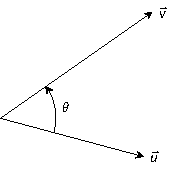
\includegraphics{figures/figdotpangle}\\
(a)\\[15pt]
\myincludegraphicsthree{width=125pt,3Dmenu,activate=onclick,deactivate=onclick,
3Droll=0,
3Dortho=0.0045,
3Dc2c=.54 .61 .58,
3Dcoo=0 0 40,
3Droo=170,
3Dlights=Headlamp,add3Djscript=asylabels.js}{}{figures/figdotpangle3D}\\
%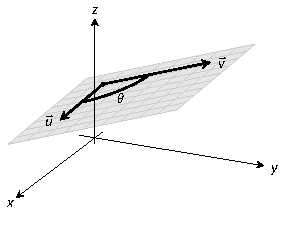
\includegraphics{figures/figdotpangle3D}\\
(b)
\end{tabular}
}

The same is also true of 2 vectors in space: given $\vec u$ and $\vec v$ in $\mathbb{R}^3$ with the same initial point, there is a plane that contains both $\vec u$ and $\vec v$. (When $\vec u$ and $\vec v$ are co-linear, there are infinite planes that contain both vectors.) In that plane, we can again find an angle $\theta$ between them (and again, $0\leq \theta\leq \pi$). This is illustrated in Figure \ref{fig:dotpangle}(b).

The following theorem connects this angle $\theta$ to the dot product of $\vec u$ and $\vec v$.

\theorem{thm:dot_product}{The Dot Product and Angles}
{Let $\vec u$ and $\vec v$ be vectors in $\mathbb{R}^2$ or $\mathbb{R}^3$. Then 
$$\dotp uv = \norm{\vec u}\,\norm{\vec v} \cos\theta,$$
where $\theta$, $0\leq\theta\leq \pi$, is the angle between $\vec u$ and $\vec v$.
\index{dot product!properties}\index{vectors!dot product}
}

When $\theta$ is an acute angle (i.e., $0\leq \theta <\pi/2$), $\cos \theta$ is positive; when $\theta = \pi/2$, $\cos \theta = 0$; when $\theta$ is an obtuse angle ($\pi/2<\theta \leq \pi$), $\cos \theta$ is negative. Thus the sign of the dot product gives a general indication of the angle between the vectors, illustrated in Figure \ref{fig:dotpsign}.

\begin{center}
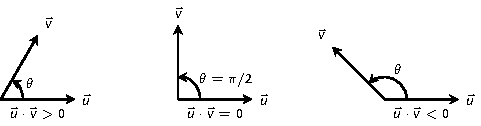
\includegraphics{figures/figdotpanglesign}
\captionsetup{type=figure}
\caption{Illustrating the relationship between the angle between vectors and the sign of their dot product.}
\label{fig:dotpsign}
\end{center}
\vskip\baselineskip

We \emph{can} use Theorem \ref{thm:dot_product} to compute the dot product, but generally this theorem is used to find the angle between known vectors (since the dot product is generally easy to compute). To this end, we rewrite the theorem's equation as
$$\cos \theta = \frac{\dotp uv}{\norm{\vec u}\norm{\vec v}} \quad \Leftrightarrow \quad \theta = \cos^{-1}\left(\frac{\dotp uv}{\norm{\vec u}\norm{\vec v}}\right).$$

We practice using this theorem in the following example.\\

\mfigure{.3}{Vectors used in Example \ref{ex_dotp2}.}{fig:dotp2}{figures/figdotp2}
\example{ex_dotp2}{Using the dot product to find angles}{
Let $\vec u = \la 3,1\ra$, $\vec v = \la -2,6\ra$ and $\vec w = \la -4,3\ra$, as shown in Figure \ref{fig:dotp2}. Find the angles $\alpha$, $\beta$ and $\theta$.
}
{We start by computing the magnitude of each vector.
$$\norm{\vec u} = \sqrt{10};\quad \norm{\vec v} = 2\sqrt{10};\quad \norm{\vec w} = 5.$$
We now apply Theorem \ref{thm:dot_product} to find the angles.
\begin{align*}
\alpha &= \cos^{-1}\left(\frac{\dotp uv}{(\sqrt{10})(2\sqrt{10})}\right) \\
			&= \cos^{-1}(0) = \frac{\pi}2 = 90^\circ.
\end{align*}
\begin{align*}
\beta &= \cos^{-1}\left(\frac{\dotp vw}{(2\sqrt{10})(5)}\right) \\
			&= \cos^{-1}\left(\frac{26}{10\sqrt{10}}\right) \\
					&\approx 0.6055 \approx 34.7^\circ.\\[10pt]
\theta &= \cos^{-1}\left(\frac{\dotp uw}{(\sqrt{10})(5)}\right) \\
				&= \cos^{-1}\left(\frac{-9}{5\sqrt{10}}\right) \\
				&\approx 2.1763 \approx 124.7^\circ
\end{align*}
\vskip-\baselineskip
}\\

We see from our computation that $\alpha + \beta = \theta$, as indicated by Figure \ref{fig:dotp2}. While we knew this should be the case, it is nice to see that this non-intuitive formula indeed returns the results we expected.

We do a similar example next in the context of vectors in space.\\

\mfigurethree{width=150pt,3Dmenu,activate=onclick,deactivate=onclick,
3Droll=0,
3Dortho=0.0045,
3Dc2c=.89 .4 .23,
3Dcoo=10 50 46,
3Droo=200,
3Dlights=Headlamp,add3Djscript=asylabels.js}{}{.4}{Vectors used in Example \ref{ex_dotp3}.}{fig:dotp3}{figures/figdotp3}%
%\mfigure{.4}{Vectors used in Example \ref{ex_dotp3}.}{fig:dotp3}{figures/figdotp3}
\example{ex_dotp3}{Using the dot product to find angles}{
Let $\vec u = \la 1,1,1\ra$, $\vec v = \la -1,3,-2\ra$ and $\vec w = \la -5,1,4\ra$, as illustrated in Figure \ref{fig:dotp3}. Find the angle between each pair of vectors.}
{\begin{enumerate}
	\item Between $\vec u$ and $\vec v$:
	\begin{align*}
	\theta &= \cos^{-1}\left(\frac{\dotp uv}{\norm{\vec u}\norm{\vec v}}\right)\\
					&= \cos^{-1}\left(\frac{0}{\sqrt{3}\sqrt{14}}\right)\\
					&= \frac{\pi}2.
	\end{align*}
	\item	Between $\vec u$ and $\vec w$:
	\begin{align*}
	\theta &= \cos^{-1}\left(\frac{\dotp uw}{\norm{\vec u}\norm{\vec w}}\right)\\
					&= \cos^{-1}\left(\frac{0}{\sqrt{3}\sqrt{42}}\right)\\
					&= \frac{\pi}2.
	\end{align*}
	\item	Between $\vec v$ and $\vec w$:
	\begin{align*}
	\theta &= \cos^{-1}\left(\frac{\dotp vw}{\norm{\vec v}\norm{\vec w}}\right)\\
					&= \cos^{-1}\left(\frac{0}{\sqrt{14}\sqrt{42}}\right)\\
					&= \frac{\pi}2.
	\end{align*}
\end{enumerate}
While our work shows that each angle is $\pi/2$, i.e.,  $90^\circ$, none of these angles looks to be a right angle in Figure \ref{fig:dotp3}. Such is the case when drawing three--dimensional objects on the page.
}\\

All three angles between these vectors was $\pi/2$, or $90^\circ$. We know from geometry and everyday life that $90^\circ$ angles are ``nice'' for a variety of reasons, so it should seem significant that these angles are all $\pi/2$. Notice the common feature in each calculation (and also the calculation of $\alpha$ in Example \ref{ex_dotp2}): the dot products of each pair of angles was 0. We use this as a basis for a definition of the term \textbf{orthogonal}, which is essentially synonymous to \textit{perpendicular}.

\definition{def:orthogonal}{Orthogonal}
{Vectors $\vec u$ and $\vec v$ are \textbf{orthogonal} if their dot product is 0.
\index{orthogonal}\index{perpendicular|see{orthogonal}}\index{vectors!orthogonal}
}

\mnote{.4}{\textbf{Note:} The term \textit{perpendicular} originally referred to lines. As mathematics progressed, the concept of ``being at right angles to'' was applied to other objects, such as vectors and planes, and the term \emph{orthogonal} was introduced. It is especially used when discussing objects that are hard, or impossible, to visualize: two vectors in 5-dimensional space are orthogonal if their dot product is 0. It is not wrong to say they are \textit{perpendicular}, but common convention gives preference to the word \textit{orthogonal}.
}

\example{ex_dotp8}{Finding orthogonal vectors}{
Let $\vec u = \la 3,5\ra$ and $\vec v = \la 1,2,3\ra$. 
\begin{enumerate}
	\item Find two vectors in $\mathbb{R}^2$ that are orthogonal to $\vec u$.
	\item	Find two non--parallel vectors in $\mathbb{R}^3$ that are orthogonal to $\vec v$.
\end{enumerate}
}
{\begin{enumerate}
	\item Recall that a line perpendicular to a line with slope $m$ has slope $-1/m$, the ``opposite reciprocal slope.'' We can think of the slope of $\vec u$ as $5/3$, its ``rise over run.'' A vector orthogonal to $\vec u$ will have slope $-3/5$. There are many such choices, though all parallel:
	$$\la -5,3\ra \quad \text{or} \quad\la 5,-3\ra \quad \text{or} \quad \la -10,6\ra\quad \text{or} \quad \la 15,-9\ra,\text{etc.}$$
	\item		There are infinite directions in space orthogonal to any given direction, so there are an infinite number of non--parallel vectors orthogonal to $\vec v$. Since there are so many, we have great leeway in finding some.
	
	One way is to arbitrarily pick values for the first two components, leaving the third unknown. For instance, let $\vec v_1 = \la 2,7,z\ra$. If $\vec v_1$ is to be orthogonal to $\vec v$, then $\vec v_1\cdot\vec v = 0$, so 
	$$2+14+3z=0 \quad \Rightarrow z = \frac{-16}{3}.$$
	So $\vec v_1 = \la 2, 7, -16/3\ra$ is orthogonal to $\vec v$. We can apply a similar technique by leaving the first or second component unknown.
	
	Another method of finding a vector orthogonal to $\vec v$ mirrors what we did in part 1. Let $\vec v_2 = \la-2,1,0\ra$. Here we switched the first two components of $\vec v$, changing the sign of one of them (similar to the ``opposite reciprocal'' concept before). Letting the third component be 0 effectively ignores the third component of $\vec v$, and it is easy to see that 
	$$\vec v_2\cdot\vec v = \la -2,1,0\ra\cdot\la 1,2,3\ra = 0.$$
	Clearly $\vec v_1$ and $\vec v_2$ are not parallel.
\end{enumerate}
\vskip-1.5\baselineskip
}\\

An important construction is illustrated in Figure \ref{fig:dotpproj}, where vectors $\vec u$ and $\vec v$ are sketched. In part (a), a dotted line is drawn from the tip of $\vec u$ to the line containing $\vec v$, where the dotted line is orthogonal to $\vec v$. In part (b), the dotted line is replaced with the vector $\vec z$ and  $\vec w$ is formed, parallel to $\vec v$. It is clear by the diagram that $\vec u = \vec w+\vec z$. What is important about this construction is this: $\vec u$ is \emph{decomposed} as the sum of two vectors, one of which is parallel to $\vec v$ and one that is perpendicular to $\vec v$. It is hard to overstate the importance of this construction (as we'll see in upcoming examples). 

The vectors $\vec w$, $\vec z$ and $\vec u$ as shown in Figure \ref{fig:dotpproj} (b) form a right triangle, where the angle between $\vec v$ and $\vec u$ is labeled $\theta$. We can find $\vec w$ in terms of $\vec v$ and $\vec u$.

Using trigonometry, we can state that 
\begin{equation}
\norm{\vec w} = \norm{\vec u}\cos \theta. \label{eq:proj1}
\end{equation}
\mtable{.450}{Developing the construction of the \emph{orthogonal projection}.}{fig:dotpproj}{%
\begin{tabular}{c}
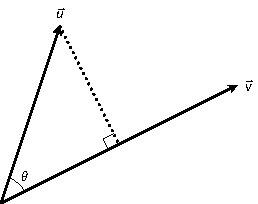
\includegraphics{figures/figdotpproja}\\
(a)\\[15pt]
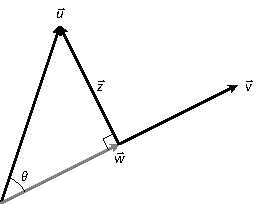
\includegraphics{figures/figdotpprojb}\\
(b)
\end{tabular}
}

We also know that $\vec w$ is parallel to to $\vec v$\,; that is, the direction of $\vec w$ is the direction of $\vec v$, described by the unit vector $\frac{1}{\norm{\vec v}}\vec v$. The vector $\vec w$ is the vector in the direction $\frac{1}{\norm{\vec v}}\vec v$ with magnitude $\norm{\vec u}\cos \theta$:
\begin{align*}
\vec w &= \Big(\norm{\vec u}\cos\theta \Big)\frac{1}{\norm{\vec v}}\vec v.
\intertext{Replace $\cos\theta$ using Theorem \ref{thm:dot_product}:}
			&= \left(\norm{\vec u}\frac{\dotp uv}{\norm{\vec u}\norm{\vec v}}\right)\frac{1}{\norm{\vec v}} \vec v\\ 
			&= \frac{\dotp uv}{\norm{\vec v}^2}\vec v.
			\intertext{Now apply Theorem \ref{thm:dot_product_properties}.}
			&= \frac{\dotp uv}{\dotp vv}\vec v.
\end{align*}

Since this construction is so important, it is given a special name.

\definition{def:orthogonal_projection}{Orthogonal Projection}
{Let $\vec u$ and $\vec v$ be given. The \textbf{orthogonal projection of $\vec u$ onto $\vec v$}, denoted $\proj uv$, is 
\index{orthogonal projection}\index{vectors!orthogonal projection}
$$\proj uv = \frac{\dotp uv}{\dotp vv}\vec v.$$
}

\example{ex_dotp4}{Computing the orthogonal projection}{
\begin{enumerate}
	\item Let $\vec u= \la -2,1\ra$ and $\vec v=\la 3,1\ra$. Find $\proj uv$, and sketch all three vectors with initial points at the origin.
	\item	Let $\vec w = \la 2,1,3\ra$ and $\vec x = \la 1,1,1\ra$. Find $\proj wx$, and sketch all three vectors with initial points at the origin.
\end{enumerate}
}
{\begin{enumerate}
	\item Applying Definition \ref{def:orthogonal_projection}, we have
	\begin{align*}
	\proj uv &= \frac{\dotp uv}{\dotp vv}\vec v \\
					&= \frac{-5}{10}\la 3,1\ra\\
					&= \la -\frac32,-\frac12\ra.
	\end{align*}
	Vectors $\vec u$, $\vec v$ and $\proj uv$ are sketched in Figure \ref{fig:dotp4}(a). Note how the projection is parallel to $\vec v$; that is, it lies on the same line through the origin as $\vec v$, although it points in the opposite direction. That is because the angle between $\vec u$ and $\vec v$ is obtuse (i.e., greater than $90^\circ$).
\mtable{.63}{Graphing the vectors used in Example \ref{ex_dotp4}.}{fig:dotp4}{%
\begin{tabular}{c}
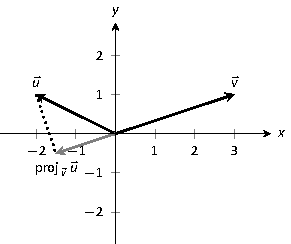
\includegraphics{figures/figdotp4a}\\
(a)\\[15pt]
\myincludegraphicsthree{width=100pt,3Dmenu,activate=onclick,deactivate=onclick,
3Droll=0,
3Dortho=0.0046,
3Dc2c=.9 .12 .42,
3Dcoo=0 50 30,
3Droo=250,
3Dlights=Headlamp,add3Djscript=asylabels.js}{}{figures/figdotp4b}\\
%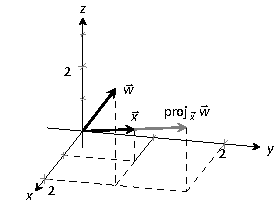
\includegraphics{figures/figdotp4b}\\
(b)\\[15pt]
\myincludegraphicsthree{width=100pt,3Dmenu,activate=onclick,deactivate=onclick,
3Droll=0,
3Dortho=0.0046,
3Dc2c=.29 .77 .56,
3Dcoo=50 0 40,
3Droo=250,
3Dlights=Headlamp,add3Djscript=asylabels.js}{}{figures/figdotp4c}\\
%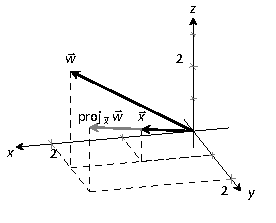
\includegraphics{figures/figdotp4c}\\
(c)\\[15pt]
\end{tabular}
}	
	
	\item		Apply the definition:
	\begin{align*}
	\proj wx &= \frac{\dotp wx}{\dotp xx}\vec x \\
					&= \frac{6}{3}\la 1,1,1\ra\\
					&= \la 2,2,2\ra.
	\end{align*}
	These vectors are sketched in Figure \ref{fig:dotp4}(b), and again in part (c) from a different perspective. Because of the nature of graphing these vectors, the sketch in part (b) makes it difficult  to recognize that the drawn projection has the geometric properties it should. The graph shown in part (c) illustrates these properties better.
\end{enumerate}
\vskip-\baselineskip
}\\

\mfigure{.23}{Illustrating the orthogonal projection.}{fig:dotpprojc}{figures/figdotpprojc}
Consider Figure \ref{fig:dotpprojc} where the concept of the orthogonal projection is again illustrated. It is clear that 
\begin{equation}
\vec u = \proj uv + \vec z.
\label{eq:orthogproj}
\end{equation} As we know what $\vec u$ and $\proj uv$ are, we can solve for $\vec z$ and state that
$$\vec z = \vec u - \proj uv.$$
This leads us to rewrite Equation \eqref{eq:orthogproj} in a seemingly silly way: $$\vec u = \proj uv + (\vec u - \proj uv).$$
This is not nonsense, as pointed out in the following Key Idea. (Notation note: the expression ``$\parallel \vec y$\,'' means ``is parallel to $\vec y$.'' We can use this notation to state ``$\vec x\parallel\vec y$\,'' which means ``$\vec x$ is parallel to $\vec y$.'' The expression ``$\perp \vec y$\,'' means ``is orthogonal to $\vec y$,'' and is used similarly.)

\keyidea{idea:orthog_proj}{Orthogonal Decomposition of Vectors}
{Let $\vec u$ and $\vec v$ be given. Then $\vec u$ can be written as the sum of two vectors, one of which is parallel to $\vec v$, and one of which is orthogonal to $\vec v$:
\index{orthogonal decomposition of vectors}\index{orthogonal!decomposition}\index{vectors!orthogonal decomposition}
$$\vec u = \underbrace{\proj uv}_{\parallel\ \vec v}\ +\  (\underbrace{\vec u-\proj uv}_{\perp\ \vec v}).$$
}

We illustrate the use of this equality in the following example.\\

\example{ex_dotp5}{Orthogonal decomposition of vectors}{
\begin{enumerate}
	\item Let $\vec u = \la -2,1\ra $ and $\vec v = \la 3,1\ra$ as in Example \ref{ex_dotp4}. Decompose $\vec u$ as the sum of a vector parallel to $\vec v$ and a vector orthogonal to $\vec v$.
	\item	Let $\vec w =\la 2,1,3\ra$ and $\vec x  =\la 1,1,1\ra$ as in Example \ref{ex_dotp4}. Decompose $\vec w$ as the sum of a vector parallel to $\vec x$ and a vector orthogonal to $\vec x$.
\end{enumerate}
}
{\begin{enumerate}
	\item In Example \ref{ex_dotp4}, we found that $\proj uv = \la -1.5,-0.5\ra$. Let $$\vec z = \vec u - \proj uv = \la -2,1\ra - \la -1.5,-0.5\ra = \la-0.5, 1.5\ra.$$
	Is $\vec z$ orthogonal to $\vec v$\,? (I.e, is $\vec z \perp\vec v$\ ?) We check for orthogonality with the dot product:
	$$\dotp zv = \la -0.5,1.5\ra \cdot \la 3,1\ra =0.$$
	Since the dot product is 0, we know $\vec z \perp \vec v$. Thus:
	\begin{align*}
	\vec u &= \proj uv\ +\ (\vec u - \proj uv) \\
	\la -2,1\ra &= \underbrace{\la -1.5,-0.5\ra}_{\parallel\ \vec v}\ +\ \underbrace{\la -0.5,1.5\ra}_{\perp \ \vec v}.
	\end{align*}
	
	\item	We found in Example \ref{ex_dotp4} that $\proj wx = \la 2,2,2\ra$. Applying the Key Idea, we have:
	$$\vec z = \vec w - \proj wx = \la 2,1,3\ra  - \la 2,2,2\ra = \la 0,-1,1\ra.$$ We check to see if $\vec z \perp \vec x$:
	$$\dotp zx = \la 0,-1,1\ra \cdot \la 1,1,1\ra = 0.$$
	Since the dot product is 0, we know the two vectors are orthogonal.
	We now write $\vec w$ as the sum of two vectors, one parallel and one orthogonal to $\vec x$:
	\begin{align*}
	\vec w &= \proj wx\ +\ (\vec w - \proj wx) \\
	\la 2,1,3\ra &= \underbrace{\la 2,2,2\ra}_{\parallel\ \vec x}\ +\ \underbrace{\la 0,-1,1\ra}_{\perp \ \vec x} 
	\end{align*}
\end{enumerate}
\vskip-\baselineskip
}\\

We give an example of where this decomposition is useful.\\

\example{ex_dotp6}{Orthogonally decomposing a force vector}{
Consider Figure \ref{fig:dotp6}(a), showing a box weighing 50lb on a ramp that rises 5ft over a span of 20ft. Find the components of force, and their magnitudes, acting on the box (as sketched in part (b) of the figure):
\mtable{.4}{Sketching the ramp and box in Example \ref{ex_dotp6}. Note: \textit{The vectors are not drawn to scale.}}{fig:dotp6}{%
\begin{tabular}{c}
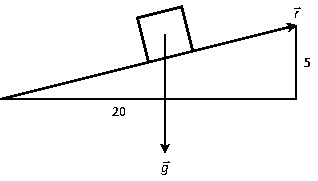
\includegraphics{figures/figdotp6}\\
(a)\\[15pt]
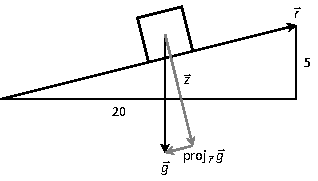
\includegraphics{figures/figdotp6b}\\
(b)
\end{tabular}
}
\begin{enumerate}
	\item in the direction of the ramp, and
	\item	orthogonal to the ramp.
\end{enumerate}
}
{As the ramp rises 5ft over a horizontal distance of 20ft, we can represent the direction of the ramp with the vector $\vec r= \la 20,5\ra$. Gravity pulls down with a force of 50lb, which we represent with $\vec g = \la 0,-50\ra$. 
\begin{enumerate}
	\item To find the force of gravity in the direction of the ramp, we compute $\proj gr$:
	\begin{align*}
	\proj gr &= \frac{\dotp gr}{\dotp rr}\vec r\\
					&=  \frac{-250}{425}\la 20,5\ra\\
					&= \la -\frac{200}{17},-\frac{50}{17}\ra \approx \la -11.76,-2.94\ra.
	\end{align*}
	The magnitude of $\proj gr$ is $\norm{\proj gr} = 50/\sqrt{17} \approx 12.13\text{lb}$. Though the box weighs 50lb, a force of about 12lb is enough to keep the box from sliding down the ramp.
	
	\item		To find the component $\vec z$ of gravity orthogonal to the ramp, we use Key Idea \ref{idea:orthog_proj}.
	\begin{align*}
	\vec z &= \vec g - \proj gr \\
					&= \la \frac{200}{17},-\frac{800}{17}\ra \approx \la 11.76,-47.06\ra.
	\end{align*}
	The magnitude of this force is $\norm{\vec z} \approx 48.51$lb. In physics and engineering, knowing this force is important when computing things like static frictional force. (For instance, we could easily compute if the static frictional force alone was enough to keep the box from sliding down the ramp.)
\end{enumerate}
\vskip-\baselineskip
}\\

\noindent\textbf{\large Application to Work}\\

In physics, the application of a force $F$ to move an object in a straight line a distance $d$ produces \emph{work}; the amount of work $W$ is $W=Fd$, (where $F$ is in the direction of travel). The orthogonal projection allows us to compute work when the force is not in the direction of travel.

\mfigure{.6}{Finding work when the force and direction of travel are given as vectors.}{fig:dotpwork}{figures/figdotpwork}
Consider Figure \ref{fig:dotpwork}, where a force $\vec F$ is being applied to an object moving in the direction of $\vec d$. (The distance the object travels is the magnitude of $\vec d$.) The work done is the amount of force in the direction of $\vec d$, $\norm{\proj Fd}$, times $\vnorm d$:
\begin{align*}
\norm{\proj Fd}\cdot\vnorm d &= \snorm{\frac{\dotp Fd}{\dotp dd}\vec d}\cdot \vnorm d \\
		&= \left|\frac{\dotp Fd}{\vnorm d^2}\right|\cdot \vnorm d\cdot\vnorm d\\
		&= \frac{\left|\dotp Fd\right|}{\vnorm d^2}\vnorm d^2\\
		&= \left|\dotp Fd\right|.
\end{align*}

The expression $\dotp Fd$ will be positive if the angle between $\vec F$ and $\vec d$ is acute; when the angle is obtuse (hence $\dotp Fd$ is negative), the force is causing motion in the opposite direction of $\vec d$, resulting in ``negative work.'' We want to capture this sign, so we drop the absolute value and find that $W = \dotp Fd$.

\definition{def:work}{Work}
{Let $\vec F$ be a constant force that moves an object in a straight line from point $P$ to point $Q$. Let $\vec d = \vv{PQ}$. The \textbf{work} $W$ done by $\vec F$ along $\vec d$ is $W = \dotp Fd$.
\index{work}
}

\example{ex_dotp7}{Computing work}{
A man slides a box along a ramp that rises 3ft over a distance of 15ft by applying 50lb of force as shown in Figure \ref{fig:dotp7}. Compute the work done.}
{The figure indicates that the force applied makes a $30^\circ$ angle with the horizontal, so $\vec F = 50\la \cos 30^\circ,\sin 30^\circ\ra \approx \la 43.3,25\ra.$ The ramp is represented by $\vec d  = \la 15,3\ra$. The work done is simply
$$\dotp Fd = 50\la \cos 30^\circ,\sin 30^\circ\ra \cdot \la 15,3\ra \approx 724.5 \text{ft--lb}.$$

\mfigure{.8}{Computing work when sliding a box up a ramp in Example \ref{ex_dotp7}.}{fig:dotp7}{figures/figdotp7}
Note how we did not actually compute the distance the object traveled, nor the magnitude of the force in the direction of travel; this is all inherently computed by the dot product!
}\\

The dot product is a powerful way of evaluating computations that depend on angles without actually using angles. The next section explores another ``product'' on vectors, the \emph{cross product.} Once again, angles play an important role, though in a much different way.

\printexercises{exercises/10_03_exercises}

%\section{The Cross Product}\label{sec:cross_product}

``Orthogonality'' is immensely important. A quick scan of your current environment will undoubtedly reveal numerous surfaces and edges that are perpendicular to each other (including the edges of this page). The dot product provides a quick test for orthogonality:  vectors $\vec u$ and $\vec v$ are perpendicular if, and only if, $\dotp uv=0$. 

Given two non--parallel, nonzero vectors $\vec u$ and $\vec v$ in space, it is very useful to find a vector $\vec w$ that is perpendicular to both $\vec u$ and $\vec v$. There is a operation, called the \textbf{cross product}, that creates such a vector. This section defines the cross product, then explores its properties and applications.

\definition{def:cross_product}{Cross Product}
{Let $\vec u =\la u_1,u_2,u_3\ra$ and $\vec v = \la v_1,v_2,v_3\ra$ be vectors in $\mathbb{R}^3$. The \textbf{cross product of $\vec u$ and $\vec v$}, denoted $\crossp uv$, is the vector
\index{vectors!cross product}\index{cross product!definition}
$$\crossp uv = \la u_2v_3-u_3v_2,-(u_1v_3-u_3v_1),u_1v_2-u_2v_1\ra.$$
}

This definition can be a bit cumbersome to remember. After an example we will give a convenient method for computing the cross product. For now, careful examination of the products and differences given in the definition should reveal a pattern that is not too difficult to remember. (For instance, in the first component only 2 and 3 appear as subscripts; in the second component, only 1 and 3 appear as subscripts. Further study reveals the order in which they appear.)

Let's practice using this definition by computing a cross product.\\

\example{ex_crossp1}{Computing a cross product}{
Let $\vec u = \la 2,-1,4\ra$ and $\vec v = \la 3,2,5\ra$. Find $\crossp uv$, and verify that it is orthogonal to both $\vec u$ and $\vec v$.
}
{Using Definition \ref{def:cross_product}, we have
$$\crossp uv = \la (-1)5-(4)2,-\big((2)5-(4)3\big), (2)2-(-1)3\ra = \la -13,2,7\ra.$$ 
(We encourage the reader to compute this product on their own, then verify their result.)

\enlargethispage{2\baselineskip}
We test whether or not $\crossp uv$ is orthogonal to $\vec u$ and $\vec v$ using the dot product:
$$\big(\crossp uv\big) \cdot \vec u = \la -13,2,7\ra \cdot \la 2,-1,4\ra = 0,$$
$$\big(\crossp uv\big) \cdot \vec v = \la -13,2,7\ra \cdot \la 3,2,5 \ra = 0.$$
Since both dot products are zero, $\crossp uv$ is indeed orthogonal to both $\vec u$ and $\vec v$.
}\\

A convenient method of computing the cross product starts with forming a particular $3\times 3$ \emph{matrix}, or rectangular array. The first row comprises the standard unit vectors $\vec i$, $\vec j$, and $\vec k$. The second and third rows are the vectors $\vec u$ and $\vec v$, respectively. Using $\vec u$ and $\vec v$ from Example \ref{ex_crossp1}, we begin with:

\btz [baseline=-3pt,>=stealth]
\node at (0,0) {$\begin{array}{ccc} \veci&\vecj&\veck \\  2&-1&4\\3&2&5\end{array}$};
\etz

Now repeat the first two columns after the original three:
\btz [baseline=-3pt,>=stealth]
\node at (0,0) {$\begin{array}{ccccc} \veci&\vecj&\veck&\veci&\vecj \\  2&-1&4&2&-1\\3&2&5&3&2\end{array}$};
\etz

This gives three full ``upper left to lower right'' diagonals, and three full ``upper right to lower left'' diagonals, as shown. Compute the products along each diagonal, then add the products on the right and subtract the products on the left:

\btz [baseline=-3pt,>=stealth]
\node at (0,0) {$\begin{array}{ccccc} \ \veci\ &\ \vecj\ &\ \veck\ &\ \veci\ &\ \vecj\ \\  2&-1&4&2&-1\\3&2&5&3&2\end{array}$};
\draw[->,  thin] (-1.3,.4) -- (.5,-.8) node[below right] {$-5\veci$};
\draw[->,  thin] (-.7,.4) -- (1.3,-.8) node[below right ] {12\vecj};
\draw[->, thin] (0,.4) -- (2,-.8) node[below right] {4\veck};
\draw[->, thin] (0,.4) -- (-2,-.8) node[below left] {$-3\veck$};
\draw[->, thin] (.7,.4) -- (-1.3,-.8) node[below left ] {8\veci};
\draw[->, thin] (1.3,.4) -- (-.5,-.8) node[below left] {10\vecj};
\etz
$$\crossp uv = \big(-5\veci+12\vecj+4\veck\,\big) - \big(-3\veck+8\veci+10\vecj\,\big) = -13\veci+2\vecj+7\veck = \la -13,2,7\ra.$$

We practice using this method.\\

\example{ex_crossp2}{Computing a cross product}{
Let $\vecu=\la 1,3,6\ra$ and $\vec v = \la -1,2,1\ra$. Compute both $\crossp uv$ and $\crossp vu$.}
{To compute $\crossp uv$, we form the matrix as prescribed above, complete with repeated first columns:
$$\begin{array}{ccccc} \ \veci\ &\ \vecj\ &\ \veck\ &\ \veci\ &\ \vecj\ \\  1&3&6&1&3\\-1&2&1&-1&2\end{array}$$
We let the reader compute the products of the diagonals; we give the result:
$$\crossp uv = \big(3\veci-6\vecj+2\veck\,\big) - \big(-3\veck + 12\veci+\vecj\,\big) = \la -9,-7,5\ra.$$

To compute $\crossp vu$, we switch the second and third rows of the above matrix, then multiply along diagonals and subtract:

$$\begin{array}{ccccc} \ \veci\ &\ \vecj\ &\ \veck\ &\ \veci\ &\ \vecj\ \\-1&2&1&-1&2\\  1&3&6&1&3\end{array}$$
Note how with the rows being switched, the products that once appeared on the right now appear on the left, and vice--versa. Thus the result is:
$$\crossp vu = \big(12\veci+\vecj-3\veck\,\big) - \big(2\veck + 3\veci-6\vecj\,\big) = \la 9,7,-5\ra,$$
which is the opposite of $\crossp uv$. We leave it to the reader to verify that each of these vectors is orthogonal to $\vec u$ and $\vec v$.
}\\

\noindent\textbf{\large Properties of the Cross Product}\\

It is not coincidence that $\crossp vu = -(\crossp uv)$ in the preceding example; one can show using Definition \ref{def:cross_product} that this will always be the case. The following theorem states several useful properties of the cross product, each of which can be verified by referring to the definition.

\setboxwidth{15pt}
%\noindent\hskip-50pt\begin{minipage}{\linewidth}
\theorem{thm:cross_prod_prop}{Properties of the Cross Product}
{Let $\vecu$, $\vecv$ and $\vecw$ be vectors in $\mathbb{R}^3$ and let $c$ be a scalar. The following identities hold:
\index{vectors!cross product}\index{cross product!properties}
\begin{enumerate}
	\item \parbox{167pt}{$\crossp uv = -(\crossp vu)$} Anticommutative Property
	\item	\begin{enumerate}
		\item \parbox{145pt}{$(\vec u+\vec v)\times \vecw = \crossp uw+\crossp vw$} Distributive Properties
		\item	$\vec u \times (\vec v+\vec w) = \crossp uv+\crossp uw$
	\end{enumerate}
	\item		$c(\crossp uv) = (c\vecu) \times \vec v = \vecu \times (c\vecv)$
	\item		\begin{enumerate}
		\item \parbox{145pt}{$(\crossp uv)\cdot \vecu = 0$} Orthogonality Properties
		\item	$(\crossp uv)\cdot \vecv = 0$
	\end{enumerate}
	\item		$\crossp uu = \vec 0$
	\item		$\crossp u0 = \vec 0$
	\item		\parbox{167pt}{$\vecu \cdot (\vecv\times\vecw) = (\crossp uv)\cdot \vecw$} Triple Scalar Product
\end{enumerate}
}
%\end{minipage}
\restoreboxwidth

We introduced the cross product as a way to find a vector orthogonal to two given vectors, but we did not give a proof that the construction given in Definition \ref{def:cross_product} satisfies this property. Theorem \ref{thm:cross_prod_prop} asserts this property holds; we leave it as a problem in the Exercise section to verify this.

Property 5 from the theorem is also left to the reader to prove in the Exercise section, but it reveals something more interesting than ``the cross product of a vector with itself is $\vec 0$.'' Let $\vec u$ and $\vec v$ be parallel vectors; that is, let there be a scalar $c$ such that $\vecv = c\vecu$. Consider their cross product:
\begin{align*}
\crossp uv &= \vecu \times (c\vec u) \\
					&=	\parbox{50pt}{$c(\crossp uu)$}\text{(by Property 3 of Theorem \ref{thm:cross_prod_prop})}\\
					&= \parbox{50pt}{$\vec 0$.}\text{(by Property 5 of Theorem \ref{thm:cross_prod_prop})}
\end{align*}

We have just shown that the cross product of parallel vectors is $\vec 0$. This hints at something deeper. Theorem \ref{thm:dot_product} related the angle between two vectors and their dot product; there is a similar relationship relating the cross product of two vectors and the angle between them, given by the following theorem.

\theorem{thm:cross_product}{The Cross Product and Angles}
{Let $\vec u$ and $\vec v$ be vectors in $\mathbb{R}^3$. Then
$$\norm{\crossp uv} = \vnorm u\, \vnorm v \sin\theta,$$
where $\theta$, $0\leq \theta \leq \pi$, is the angle between $\vecu$ and $\vecv$.
\index{vectors!cross product}\index{cross product!properties}
}

\mnote{.52}{\textbf{Note:} Definition \ref{def:orthogonal} (through Theorem \ref{thm:dot_product}) defines $\vec u$ and $\vec v$ to be orthogonal if $\vec u\cdot\vec v=0$. We could use Theorem \ref{thm:cross_product} to define $\vec u$ and $\vec v$ are parallel if $\vec u\times \vec v = 0$. By such a definition, $\vec 0$ would be both orthogonal and parallel to every vector. Apparent paradoxes such as this are not uncommon in mathematics and can be very useful. (See also the marginal note on page \pageref{note:parallel}.)\label{note:crossp}}
Note that this theorem makes a statement about the \emph{magnitude} of the cross product. When the angle between $\vecu$ and $\vecv$ is 0 or $\pi$ (i.e., the vectors are parallel), the magnitude of the cross product is 0. The only vector with a magnitude of 0 is $\vec 0$ (see Property \ref{thm:zero_norm} of Theorem \ref{thm:vector_properties}), hence the cross product of  parallel vectors is $\vec 0$.\\

We demonstrate the truth of this theorem in the following example.\\

\example{ex_crossp3}{The cross product and angles}{
Let $\vec u = \la 1,3,6\ra$ and $\vec v = \la -1,2,1\ra$ as in Example \ref{ex_crossp2}. Verify Theorem \ref{thm:cross_product} by finding $\theta$, the angle between $\vecu$ and $\vecv$, and the magnitude of $\crossp uv$.}
{We use Theorem \ref{thm:dot_product} to find the angle between $\vecu$ and $\vecv$. 
\begin{align*}
\theta &= \cos^{-1}\left(\frac{\dotp uv}{\vnorm u\, \vnorm v}\right) \\
			&= \cos^{-1}\left(\frac{11}{\sqrt{46}\sqrt{6}}\right)\\
			&\approx 0.8471 = 48.54^\circ.
\end{align*}

Our work in Example \ref{ex_crossp2} showed that $\crossp uv = \la -9,-7,5\ra$, hence $\norm{\crossp uv} = \sqrt{155}.$ Is $\norm{\crossp uv} = \vnorm u\, \vnorm v\sin\theta$? Using numerical approximations, we find:
\begin{align*}
\norm{\crossp uv} &=\sqrt{155}  & \vnorm u\,\vnorm v \sin\theta & = \sqrt{46}\sqrt{6}\sin 0.8471\\
									&\approx 12.45. & &\approx 12.45.
\end{align*}
Numerically, they seem equal. Using a right triangle, one can show that 
$$\sin\left(\cos^{-1}\left(\frac{11}{\sqrt{46}\sqrt{6}}\right)\right) = \frac{\sqrt{155}}{\sqrt{46}\sqrt{6}},$$ which allows us to verify the theorem exactly.
}\\

\noindent\textbf{Right Hand Rule}\\

The anticommutative property of the cross product demonstrates that $\crossp uv$ and $\crossp vu$ differ only by a sign -- these vectors have the same magnitude but point in the opposite direction. When seeking a vector perpendicular to $\vec u$ and $\vec v$, we essentially have two directions to choose from, one in the direction of $\crossp uv$ and one in the direction of $\crossp vu$. Does it matter which we choose? How can we tell which one we will get without graphing, etc.?

Another wonderful property of the cross product, as defined, is that it follows the \textbf{right hand rule.} Given $\vec u$ and $\vec v$ in $\mathbb{R}^3$ with the same initial point, point the index finger of your right hand in the direction of $\vecu$ and let your middle finger point in the direction of $\vecv$ (much as we did when establishing the right hand rule for the 3-dimensional coordinate system). Your thumb will naturally extend in the direction of $\crossp uv$. One can ``practice'' this using Figure \ref{fig:crossp_rhr}. If you switch, and point the index finder in the direction of $\vecv$ and the middle finger in the direction of $\vecu$, your thumb will now point in the opposite direction, allowing you to ``visualize'' the anticommutative property of the cross product.
\mfigurethree{width=150pt,3Dmenu,activate=onclick,deactivate=onclick,
3Droll=0,
3Dortho=0.0044,
3Dc2c=.78 .32 .53,
3Dcoo=0 0 34,
3Droo=150,
3Dlights=Headlamp,add3Djscript=asylabels.js}{}{.5}{Illustrating the Right Hand Rule of the cross product.}{fig:crossp_rhr}{figures/figcrossp_rhr}
%\mfigure[scale=1.25,trim=5mm 5mm 5mm 5mm,clip=true]{.5}{Illustrating the Right Hand Rule of the cross product.}{fig:crossp_rhr}{figures/figcrossp_rhr}

\vskip\baselineskip
\noindent\textbf{\large Applications of the Cross Product}\\

There are a number of ways in which the cross product is useful in mathematics, physics and other areas of science beyond ``just'' finding a vector perpendicular to two others. We highlight a few here.\index{cross product!applications}\\
%\enlargethispage{\baselineskip}
%\clearpage\enlargethispage{2\baselineskip}

\noindent\textbf{Area of a Parallelogram}\\

It is a standard geometry fact that the area of a parallelogram is $A = bh$, where $b$ is the length of the base and $h$ is the height of the parallelogram, as illustrated in Figure \ref{fig:crossp_parallelogram}(a). As shown when defining the Parallelogram Law of vector addition, two vectors $\vecu$ and $\vecv$ define a parallelogram when drawn from the same initial point, as illustrated in Figure \ref{fig:crossp_parallelogram}(b). Trigonometry tells us that $h = \vnorm u \sin \theta$, hence the area of the parallelogram is 
\begin{equation}A = \vnorm u\,\vnorm v\sin\theta = \norm{\crossp uv},\label{eq:crossp1}\end{equation}
where the second equality comes from Theorem \ref{thm:cross_product}.
\mtable{.75}{Using the cross product to find the area of a parallelogram.}{fig:crossp_parallelogram}{%
\begin{tabular}{c}
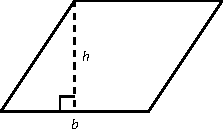
\includegraphics{figures/figcrossp_parallelogram1}\\
(a) \\[15pt]
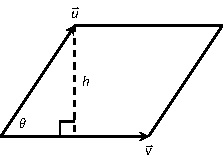
\includegraphics{figures/figcrossp_parallelogram2}\\
(b) \\
\end{tabular}
}
We illustrate using Equation \eqref{eq:crossp1} in the following example.
\index{cross product!applications!area of parallelogram}\\

\example{ex_crossp4}{Finding the area of a parallelogram}{
\begin{enumerate}
	\item Find the area of the parallelogram defined by the vectors $\vecu = \la 2,1\ra$ and $\vecv = \la 1,3\ra$.
	\item	Verify that the points $A = (1,1,1)$, $B = (2,3,2)$, $C = (4,5,3)$ and $D = (3,3,2)$ are the vertices of a parallelogram. Find the area of the parallelogram.
\end{enumerate}
}
{\begin{enumerate}
	\item Figure \ref{fig:crossp4}(a) sketches the parallelogram defined by the vectors $\vec u$ and $\vec v$. We have a slight problem in that our vectors exist in $\mathbb{R}^2$, not $\mathbb{R}^3$, and the cross product is only defined on vectors in $\mathbb{R}^3$. We skirt this issue by viewing $\vec u$ and $\vecv$ as vectors in the $x-y$ plane of $\mathbb{R}^3$, and rewrite them as $\vec u = \la 2,1,0\ra$ and $\vecv =\la 1,3,0\ra$. We can now compute the cross product. 
	It is easy to show that $\crossp uv = \la 0,0,5\ra$; therefore the area of the parallelogram is $A = \norm{\crossp uv} = 5$.
	\mtable{.35}{Sketching the parallelograms in Example \ref{ex_crossp4}.}{fig:crossp4}{%
	\begin{tabular}{c}
	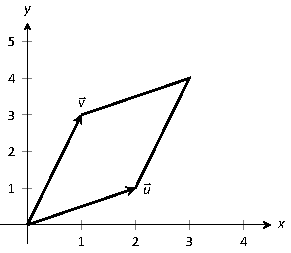
\includegraphics{figures/figcrossp4b}\\
	(a)\\[15pt]
	\myincludegraphicsthree{width=125pt,3Dmenu,activate=onclick,deactivate=onclick,
3Droll=0,
3Dortho=0.004,
3Dc2c=.42 .87 .26,
3Dcoo=61 60 63,
3Droo=250,
3Dlights=Headlamp,add3Djscript=asylabels.js}{scale=1.25,trim=4mm 5mm 4mm 5mm,clip=true}{figures/figcrossp4a}\\
	%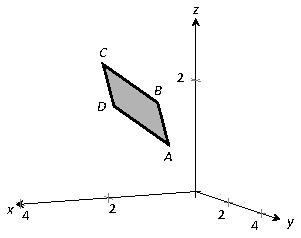
\includegraphics{figures/figcrossp4a}\\
	(b)
	\end{tabular}
	}
	\item		To show that the quadrilateral $ABCD$ is a parallelogram (shown in Figure \ref{fig:crossp4}(b)), we need to show that the opposite sides are parallel. We can quickly show that $\vv{AB} =\vv{DC} = \la 1,2,1\ra$ and $\vv{BC} = \vv{AD} = \la 2,2,1\ra$. We find the area by computing the magnitude of the cross product of $\vv{AB}$ and $\vv{BC}$:
	$$\vv{AB} \times \vv{BC} = \la 0,1,-2\ra \quad \Rightarrow \quad \norm{\vv{AB}\times\vv{BC}} = \sqrt{5} \approx 2.236.$$
\end{enumerate}
\vskip-\baselineskip
}\\

This application is perhaps more useful in finding the area of a triangle (in short, triangles are used more often than parallelograms). We illustrate this in the following example.\\

\example{ex_crossp5}{Area of a triangle}{
Find the area of the triangle with vertices $A=(1,2)$, $B=(2,3)$ and $C=(3,1)$, as pictured in Figure \ref{fig:crossp5}.}
{We found the area of this triangle in Example \ref{ex_abc4} to be $1.5$ using integration. There we discussed the fact that finding the area of a triangle can be inconvenient using the ``$\frac12bh$'' formula as one has to compute the height, which generally involves finding angles, etc. Using a cross product is much more direct.
\mfigure{.78}{Finding the area of a triangle in Example \ref{ex_crossp5}.}{fig:crossp5}{figures/figcrossp5}

We can choose any two sides of the triangle to use to form vectors; we choose $\vv{AB} = \la 1,1\ra$ and $\vv{AC}=\la 2,-1\ra$. As in the previous example, we will rewrite these vectors with a third component of 0 so that we can apply the cross product. The area of the triangle is
$$\frac12\norm{\vv{AB}\times\vv{AC}} = \frac12\norm{\la 1,1,0\ra \times \la 2,-1,0\ra} = \frac12\norm{\la 0,0,-3\ra} = \frac32.$$
We arrive at the same answer as before with less work.
}\\

\noindent\textbf{Volume of a Parallelepiped}

The three dimensional analogue to the parallelogram is the \textbf{parallelepiped}. Each face is parallel to the opposite face, as illustrated in Figure \ref{fig:crossp_parallelepiped}. By crossing $\vec v$ and $\vec w$, one gets a vector whose magnitude is the area of the base. Dotting this vector with $\vecu$ computes the volume of parallelepiped! (Up to a sign; take the absolute value.)
\mnote{.5}{\textbf{Note:} The word ``parallelepiped'' is pronounced ``parallel--eh--pipe--ed.''}
\mfigurethree{width=100pt,3Dmenu,activate=onclick,deactivate=onclick,
3Droll=0,
3Dortho=0.0045,
3Dc2c=.84 .46 .26,
3Dcoo=0 110 86,
3Droo=150,
3Dlights=Headlamp,add3Djscript=asylabels.js}{}{.35}{A parallelepiped is the three dimensional analogue to the parallelogram.}{fig:crossp_parallelepiped}{figures/figcrosspparallelpiped}
%\mfigure{.53}{A parallelepiped is the three dimensional analogue to the parallelogram.}{fig:crossp_parallelepiped}{figures/figcrosspparallelpiped}
\index{cross product!applications!volume of parallelepiped}

Thus the volume of a parallelepiped defined by vectors $\vecu$, $\vecv$ and $\vec w$ is \begin{equation}V = |\vecu\cdot (\crossp vw)|.\label{eq:crossp2}\end{equation}
Note how this is the Triple Scalar Product, first seen in Theorem \ref{thm:cross_prod_prop}. Applying the identities given in the theorem shows that we can apply the Triple Scalar Product in any ``order'' we choose to find the volume. That is,
$$V = |\vecu\cdot(\crossp vw)| = |\vec u\cdot (\crossp wv)| = |(\crossp uv)\cdot \vecw|,\quad \text{etc.}$$

\example{ex_crossp6}{Finding the volume of parallelepiped}{
Find the volume of the parallepiped defined by the vectors $\vecu = \la 1,1,0\ra$, $\vecv = \la -1,1,0\ra$ and $\vecw = \la 0,1,1\ra$. 
}
{We apply Equation \eqref{eq:crossp2}. We first find $\crossp vw =\la 1,1,-1\ra$. Then
$$|\vec u\cdot(\crossp vw)| = |\la 1,1,0\ra \cdot \la1,1,-1\ra| = 2.$$
So the volume of the parallelepiped is 2 cubic units.
\mfigurethree{width=125pt,3Dmenu,activate=onclick,deactivate=onclick,
3Droll=0,
3Dortho=0.0045,
3Dc2c=4 4 2,
3Dcoo=0 50 50,
3Droo=150,
3Dlights=Headlamp,add3Djscript=asylabels.js}{}{.8}{A parallelepiped in Example \ref{ex_crossp6}.}{fig:crossp6}{figures/figcrossp6}
%\mfigure{.3}{A parallelepiped in Example \ref{ex_crossp6}.}{fig:crossp6}{figures/figcrossp6}
}\\

While this application of the Triple Scalar Product is interesting, it is not used all that often: parallelepipeds are not a common shape in physics and engineering. The last application of the cross product is very applicable in engineering.\\

\noindent\textbf{Torque}\\

\textbf{Torque} is a measure of the turning force applied to an object. A classic scenario involving torque is the application of a wrench to a bolt. When a force is applied to the wrench, the bolt turns. When we represent the force and wrench with vectors $\vec F$ and $\vec \ell$, we see that the bolt moves (because of the threads) in a  direction orthogonal to $\vec F$ and $\vec \ell$. Torque is usually represented by the Greek letter $\tau$, or tau, and has units of N$\cdot$m, a Newton--meter, or ft$\cdot$lb, a foot--pound.\index{cross product!applications!torque}

While a full understanding of torque is beyond the purposes of this book, when a force $\vec F$ is applied to a lever arm $\vec \ell$, the resulting torque is \begin{equation}\vec \tau = \crossp \ell F.\label{eq:crossp3}\end{equation}

\example{ex_crossp7}{Computing torque}{
A lever of length 2ft makes an angle with the horizontal of $45^\circ$. Find the resulting torque when a force of 10lb is applied to the end of the level where:
\mfigure{.5}{Showing a force being applied to a lever in Example \ref{ex_crossp7}.}{fig:crossp7}{figures/figcrossp7}
\begin{enumerate}
	\item the force is perpendicular to the lever, and
	\item	the force makes an angle of $60^\circ$ with the lever, as shown in Figure \ref{fig:crossp7}.
\end{enumerate}
}
{\begin{enumerate}
	\item We start by determining vectors for the force and lever arm. Since the lever arm makes a $45^\circ$ angle with the horizontal and is 2ft long, we can state that $\vec \ell = 2\la \cos 45^\circ,\sin 45^\circ\ra = \la \sqrt2,\sqrt2\ra.$
	
	Since the force vector is perpendicular to the lever arm (as seen in the left hand side of Figure \ref{fig:crossp7}), we can conclude it is making an angle of $-45^\circ$ with the horizontal. As it has a magnitude of 10lb, we can state $\vec F = 10\la \cos (-45^\circ), \sin(-45^\circ)\ra = \la 5\sqrt2,-5\sqrt2\ra.$
	
	Using Equation \eqref{eq:crossp3} to find the torque requires a cross product. We again let the third component of each vector be 0  and compute the cross product:
	\begin{align*}
	\vec\tau &= \crossp \ell F \\
				&= \la \sqrt2,\sqrt2,0\ra \times \la 5\sqrt2,-5\sqrt2,0\ra \\
				&= \la 0,0,-20\ra
	\end{align*}
	This clearly has a magnitude of 20 ft-lb.
	
	We can view the force and lever arm vectors as lying ``on the page''; our computation of $\vec\tau$ shows that the torque goes ``into the page.'' This follows the Right Hand Rule of the cross product, and it also matches well with the example of the wrench turning the bolt. Turning a bolt clockwise moves it in.
	
	\item		Our lever arm can still be represented by $\vec \ell = \la \sqrt2,\sqrt2\ra$. As our force vector makes a $60^\circ$ angle with $\vec \ell$, we can see (referencing the right hand side of the figure) that $\vec F$ makes a $-15^\circ$ angle with the horizontal. Thus 
	\begin{align*}
	\vec F = 10\la \cos-15^\circ,\sin-15^\circ\ra &= \la \frac{5(1+\sqrt3)}{\sqrt2},\frac{5(-1+\sqrt3)}{\sqrt2}\ra \\
	&\approx \la 9.659,-2.588\ra.\end{align*}
	
	We again make the third component 0 and take the cross product to find the torque:
	\begin{align*}
	\vec\tau &= \crossp \ell F\\
					&= \la \sqrt2,\sqrt2,0\ra \times  \la \frac{5(1+\sqrt3)}{\sqrt2},\frac{5(-1+\sqrt3)}{\sqrt2},0\ra\\
					&= \la 0,0,-10\sqrt3\ra\\
					&\approx \la 0,0,-17.321\ra.
	\end{align*}
	As one might expect, when the force and lever arm vectors \textit{are} orthogonal, the magnitude of force is greater than when the vectors \textit{are not} orthogonal.
\end{enumerate}
\vskip-\baselineskip
}\\

While the cross product has a variety of applications (as noted in this chapter), its fundamental use is finding a vector perpendicular to two others. Knowing a vector is orthogonal to two others is of incredible importance, as it allows us to find the equations of lines and planes in a variety of contexts. The importance of the cross product, in some sense, relies on the importance of lines and planes, which see widespread use throughout engineering, physics and mathematics. We study lines and planes in the next two sections. 

\printexercises{exercises/10_04_exercises}


%\section{Lines}\label{sec:lines}

\index{lines}
To find the equation of a line in the $x$-$y$ plane, we need two pieces of information: a point and the slope. The slope conveys \textit{direction} information. As vertical lines have an undefined slope, the following statement is more accurate:

\begin{quotation}
\noindent To define a line, one needs a point on the line and the direction of the line.
\end{quotation}

This holds true for lines in space.\\

Let $P$ be a point in space, let $\vec p$ be the vector with initial point at the origin and terminal point at $P$ (i.e., $\vec p$ ``points'' to $P$), and let $\vec d$ be a vector. Consider the points on the line through $P$ in the direction of $\vec d$. 

Clearly one point on the line is $P$; we can say that the \emph{vector} $\vec p$ lies at this point on the line. To find another point on the line, we can start at $\vec p$ and move in a  direction parallel to $\vec d$. For instance, starting at $\vec p$ and traveling one length of $\vec d$ places one at another point on the line. Consider Figure \ref{fig:lines_intro} where certain points along the line are indicated. 
\mfigurethree{width=125pt,3Dmenu,activate=onclick,deactivate=onclick,
3Droll=0,
3Dortho=0.0045,
3Dc2c=.84 .46 .26,
3Dcoo=0 70 0,
3Droo=150,
3Dlights=Headlamp,add3Djscript=asylabels.js}{scale=1.25,trim=5mm 5mm 5mm 5mm,clip=true}{.7}{Defining a line in space.}{fig:lines_intro}{figures/figlines_intro}
%\mfigure[scale=1.25,trim=5mm 5mm 5mm 5mm,clip=true]{.7}{Defining a line in space.}{fig:lines_intro}{figures/figlines_intro}

The figure illustrates how every point on the line can be obtained by starting with $\vec p$ and moving a certain distance in the direction of $\vec d$. That is, we can define the line as a function of $t$:
\begin{equation}\vec\ell(t) = \vec p + t\ \vec d.\label{eq:lines1}\end{equation}

In many ways, this is \textit{not} a new concept. Compare Equation \eqref{eq:lines1} to the familiar ``$y=mx+b$'' equation of a line:

\begin{center}
\begin{tikzpicture}[>=stealth]
	\draw (0,0) node (L) {\large $y\ =\ b\ +\ m\,x$};
	\draw (5,0) node (R) {\large $\vec \ell(t)\ =\ \vec p\ +\ t\,\vec d$};
\node (A) at (1,1.5) [align=center,] {Starting\\ Point};
\node (B) at (4,1.5) [align=center] {Direction};
\node (C) at (2.5,-1.5) [align=center] {How Far To\\  Go In That \\Direction};
\draw [->,thick] (A) -- ($(R)+(-1pt,8pt)$);	
\draw [->,thick] (A) -- ($(L)+(-0pt,10pt)$);
\draw [->,thick] (B) -- (.9,.2);
\draw [->,thick] (B) -- ($(R)+(30pt,7pt)$);
\draw [->,thick] (C) -- (1.3,-.15);
\draw [->,thick] (C) -- ($(R)+(25pt,-7pt)$);
\end{tikzpicture}
\captionsetup{type=figure}%
\caption{Understanding the vector equation of a line.}
\label{fig:lines_eq}
\end{center}


%\begin{center}
%\begin{tikzpicture}[>=stealth]
	%\draw (0,0) node {\large $y\ =\ b\ +\ m\,x$};
%\node (A) at (-1,-1) [align=center,] {Starting\\ Point};
%\node (B) at (1,-1) [align=center] {Direction};
%\node (C) at (3,-1) [align=center] {How Far To\\  Go In That \\Direction};
%\draw [->,thick] (A) -- (-.3,-.2);	
%\draw [->,thick] (B) -- (.8,-.2);
%\draw [->,thick] (C) -- (1.3,-.15);
%\end{tikzpicture}
%\end{center}
%Now compare this to the formula given in Equation \eqref{eq:lines1}:
%\begin{center}
%\begin{tikzpicture}[>=stealth]
	%\draw (0,0) node {\large $\vec \ell(t)\ =\ \vec p\ +\ t\,\vec d$};
%\node (A) at (-1,-1) [align=center,] {Starting\\ Point};
%\node (B) at (.5,.75) [align=center] {Direction};
%\node (C) at (2,-1.25) [align=center] {How Far To\\  Go In That \\Direction};
%\draw [->,thick] (A) -- (-.05,-.2);	
%\draw [->,thick] (B) -- (1.2,.3);
%\draw [->,thick] (C) -- (1.0,-.2);
%\end{tikzpicture}
%\end{center}

The equations exhibit the same structure: they give a starting point, define a direction, and state how far in that direction to travel.

Equation \eqref{eq:lines1} is an example of a \textbf{vector--valued function}; the input of the function is a real number and the output is a vector. We will cover vector--valued functions extensively in the next chapter.

There are other ways to represent a line. Let $\vec p = \la x_0,y_0,z_0\ra$ and let $\vec d = \la a,b,c\ra$. Then the equation of the line through $\vec p$ in the direction of $\vec d$ is:
\begin{align*}
\vec\ell(t) &= \vec p + t\vec d \\
						&= \la x_0,y_0,z_0\ra + t\la a,b,c\ra \\
						&= \la x_0 + at, y_0+bt, z_0+ct\ra.
\end{align*}

The last line states that the $x$ values of the line are given by $x=x_0+at$, the $y$ values are given by $y = y_0+bt$, and the $z$ values are given by $z = z_0 + ct$. These three equations, taken together, are the \textbf{parametric equations of the line} through $\vec p$ in the direction of $\vec d$.

Finally, each of the equations for $x$, $y$ and $z$ above contain the variable $t$. We can solve for $t$ in each equation:
\begin{align*}
x = x_0+at \quad&\Rightarrow\quad t=\frac{x-x_0}{a},\\
y=y_0+bt \quad&\Rightarrow\quad t = \frac{y-y_0}{b},\\
z = z_0+ct \quad&\Rightarrow\quad t = \frac{z-z_0}{c},\\
\end{align*}
assuming $a,b,c\neq 0$.
Since $t$ is equal to each expression on the right, we can set these equal to each other, forming the \textbf{symmetric equations of the line} through $\vec p$ in the direction of $\vec d$:
$$\frac{x-x_0}{a} = \frac{y-y_0}{b}=\frac{z-z_0}{c}.$$
Each representation has its own advantages, depending on the context. We summarize these three forms in the following definition, then give examples of their use.
\clearpage

\definition{def:lines}{Equations of Lines in Space}
{Consider the line in space that passes through $\vec p = \la x_0,y_0,z_0\ra$ in the direction of $\vec d = \la a,b,c\ra.$\index{lines!equations for}
\begin{enumerate}
	\item The \textbf{vector equation} of the line is $$\vec \ell(t) = \vec p+t\vec d.$$
	\item	The \textbf{parametric equations} of the line are
	$$x = x_0+at, \quad y=y_0+bt, \quad z = z_0+ct .$$
	\item	The \textbf{symmetric equations} of the line are
	$$\frac{x-x_0}{a} = \frac{y-y_0}{b}=\frac{z-z_0}{c}.$$
\end{enumerate}
}

\example{ex_lines1}{Finding the equation of a line}{
Give all three equations, as given in Definition \ref{def:lines}, of the line through $P = (2,3,1)$ in the direction of $\vec d = \la -1,1,2\ra$. Does the point $Q=(-1,6,6)$ lie on this line?}
{We identify the point $P=(2,3,1)$ with the vector $\vec p =\la 2,3,1\ra$. Following the definition, we have
\begin{itemize}
	\item the vector equation of the line is $\vec\ell(t) = \la 2,3,1\ra + t\la -1,1,2\ra$;
	\item	the parametric equations of the line are
	$$x = 2-t,\quad y = 3+t,\quad z = 1+2t; \text{ and}$$
	\item	the symmetric equations of the line are
	$$\frac{x-2}{-1}=\frac{y-3}{1} = \frac{z-1}{2}.$$
\end{itemize}
\mfigurethree{width=125pt,3Dmenu,activate=onclick,deactivate=onclick,
3Droll=0,
3Dortho=0.0045,
3Dc2c=.78 .53 .32,
3Dcoo=0 70 50,
3Droo=150,
3Dlights=Headlamp,add3Djscript=asylabels.js}{scale=1.25,trim=2mm 2mm 2mm 2mm,clip=true}{.5}{Graphing a line in Example \ref{ex_lines1}.}{fig:lines1}{figures/figlines1}
%\mfigure[scale=1.25,trim=2mm 2mm 2mm 2mm,clip=true]{.5}{Graphing a line in Example \ref{ex_lines1}.}{fig:lines1}{figures/figlines1}

The first two equations of the line are useful when a $t$ value is given: one can immediately find the corresponding point on the line. These forms are good when calculating with a computer; most software programs easily handle equations in these formats. (For instance, the graphics program that made Figure \ref{fig:lines1} can be given the input ``\texttt{(2-t,3+t,1+2*t)}'' for $-1\leq t\leq 3$.).

Does the point $Q = (-1,6,6)$ lie on the line? The graph in Figure \ref{fig:lines1} makes it clear that it does not. We can answer this question without the graph using any of the three equation forms. Of the three, the symmetric equations are probably best suited for this task. Simply plug in the values of $x$, $y$ and $z$ and see if equality is maintained:
$$ \frac{-1-2}{-1} \stackrel{?}{=} \frac{6-3}{1} \stackrel{?}{=} \frac{6-1}{2} \quad \Rightarrow \quad 3=3\neq2.5.$$
We see that $Q$ does not lie on the line as it did not satisfy the symmetric equations.
}\\

\example{ex_lines6}{Finding the equation of a line through two points}{
Find the parametric equations of the line through the points $P=(2,-1,2)$ and $Q = (1,3,-1)$.}
{Recall the statement made at the beginning of this section: to find the equation of a line, we need a point and a direction. We have \emph{two} points; either one will suffice. The direction of the line can be found by the vector with initial point $P$ and terminal point $Q$: $\vv{PQ} = \la -1,4,-3\ra$.

The parametric equations of the line $\ell$ through $P$ in the direction of $\vv{PQ}$ are:
$$\ell: \quad x= 2-t\quad y=-1+4t \quad z=2-3t.$$
\mfigurethree{width=125pt,3Dmenu,activate=onclick,deactivate=onclick,
3Droll=0,
3Dortho=0.0045,
3Dc2c=.4 .87 .32,
3Dcoo=58 8.7 4.6,
3Droo=150,
3Dlights=Headlamp,add3Djscript=asylabels.js}{scale=1.25}{.6}{A graph of the line in Example \ref{ex_lines6}.}{fig:lines6}{figures/figlines6}
%\mfigure[scale=1.25]{.6}{A graph of the line in Example \ref{ex_lines6}.}{fig:lines6}{figures/figlines6}

A graph of the points and line are given in Figure \ref{fig:lines6}. Note how in the given parametrization of the line, $t=0$ corresponds to the point $P$, and $t=1$ corresponds to the point $Q$. This relates to the understanding of the vector equation of a line described in Figure \ref{fig:lines_eq}. The parametric equations ``start'' at the point $P$, and $t$ determines how far in the direction of $\vv{PQ}$ to travel. When $t=0$, we travel 0 lengths of $\vv{PQ}$; when $t=1$, we travel one length of $\vv{PQ}$, resulting in the point $Q$.
}\\

\noindent \textbf{\large Parallel, Intersecting and Skew Lines}\\

In the plane, two \emph{distinct} lines can either be parallel or they will intersect at exactly one point. In space, given equations of two lines, it can sometimes be difficult to tell whether the lines are distinct or not (i.e., the same line can be represented in different ways). Given lines $\vec\ell_1(t) = \vec p_1 + t\vec d_1$ and $\vec \ell_2(t) = \vec p_2+t\vec d_2$, we have four possibilities: $\vec \ell_1$ and $\vec \ell_2$ are
\index{lines!skew}\index{lines!parallel}\index{lines!intersecting}

\begin{center}
\begin{tabular}{p{100pt}p{150pt}}
the same line & they share all points; \\
intersecting lines & share only 1 point;\\
parallel lines & $\vec d_1\parallel \vec d_2$, no points in common; or \\
skew lines & $\vec d_1\nparallel \vec d_2$, no points in common. 
\end{tabular}
\end{center}

The next two examples investigate these possibilities.\\

\example{ex_lines2}{Comparing lines}{
Consider lines $\ell_1$ and $\ell_2$, given in parametric equation form:
$$\ell_1: \begin{array}{ccc} x&=&1+3t \\ y&=&2-t\\z&=&t\end{array}\qquad\qquad \ell_2:\begin{array}{ccc} x&=&-2+4s\\y&=&3+s\\z&=&5+2s.\end{array}$$
Determine whether $\ell_1$ and $\ell_2$ are the same line, intersect, are parallel, or skew.}
{We start by looking at the directions of each line. Line $\ell_1$ has the direction given by $\vec d_1=\la 3,-1,1\ra$ and line $\ell_2$ has the direction given by $\vec d_2 = \la 4,1,2\ra$. It should be clear that $\vec d_1$ and $\vec d_2$ are not parallel, hence $\ell_1$ and $\ell_2$ are not the same line, nor are they parallel. Figure \ref{fig:lines2} verifies this fact (where the points and directions indicated by the equations of each line are identified).
\mfigurethree{width=125pt,3Dmenu,activate=onclick,deactivate=onclick,
3Droll=0,
3Dortho=0.0045,
3Dc2c=.42 .80 .43,
3Dcoo=0 30 50,
3Droo=150,
3Dlights=Headlamp,add3Djscript=asylabels.js}{scale=1.25,trim=5mm 5mm 5mm 5mm,clip=true}{.6}{Sketching the lines from Example \ref{ex_lines2}.}{fig:lines2}{figures/figlines2}
%\mfigure[scale=1.25,trim=5mm 5mm 5mm 5mm,clip=true]{.6}{Sketching the lines from Example \ref{ex_lines2}.}{fig:lines2}{figures/figlines2}

We next check to see if they intersect (if they do not, they are skew lines). To find if they intersect, we look for $t$ and $s$ values such that the respective $x$, $y$ and $z$ values are the same. That is, we want $s$ and $t$ such that:
$$\begin{array}{ccc}
1+3t &=&-2+4s\\
2-t&=&3+s\\
t&=&5+2s.\end{array}$$
This is a relatively simple system of linear equations. Since the last equation is already solved for $t$, substitute that value of $t$ into the equation above it:
$$2-(5+2s) = 3+s \quad \Rightarrow \quad s=-2,\ t=1.$$
A key to remember is that we have \emph{three} equations; we need to check if $s=-2,\ t=1$ satisfies the first equation as well:
$$1+3(1) \neq -2+4(-2).$$
It does not. Therefore, we conclude that the lines $\ell_1$ and $\ell_2$ are skew.
}\\

\example{ex_lines3}{Comparing lines}{
Consider lines $\ell_1$ and $\ell_2$, given in parametric equation form:
$$\ell_1: \begin{array}{ccc} x&=&-0.7+1.6t \\ y&=&4.2+2.72t\\z&=&2.3-3.36t\end{array}\qquad\qquad \ell_2:\begin{array}{ccc} x&=&2.8-2.9s\\y&=&10.15-4.93s\\z&=&-5.05+6.09s.\end{array}$$
Determine whether $\ell_1$ and $\ell_2$ are the same line, intersect, are parallel, or skew.}
{It is obviously very difficult to simply look at these equations and discern anything. This is done intentionally. In the ``real world,'' most equations that are used do not have nice, integer coefficients. Rather, there are lots of digits after the decimal and the equations can look ``messy.''

We again start by deciding whether or not each line has the same direction. The direction of $\ell_1$ is given by $\vec d_1 = \la 1.6,2.72,-3.36\ra$ and the direction of $\ell_2$ is given by $\vec d_2 = \la -2.9,-4.93,6.09\ra$. When it is not clear through observation whether two vectors are parallel or not, the standard way of determining this is by comparing their respective unit vectors. Using a calculator, we find:
\begin{align*}
\vec u_1 &= \frac{\vec d_1}{\norm{\vec d_1}} = \la 0.3471,0.5901,-0.7289\ra\\
 \vec u_2 &= \frac{\vec d_2}{\norm{\vec d_2}} = \la -0.3471,-0.5901,0.7289\ra.
\end{align*}

\enlargethispage{\baselineskip}
The two vectors seem to be parallel (at least, their components are equal to 4 decimal places). In most situations, it would suffice to conclude that the lines are at least parallel, if not the same. One way to be sure is to rewrite $\vec d_1$ and $\vec d_2$ in terms of fractions, not decimals. We have 
$$\vec d_1 =\la \frac{16}{10},\frac{272}{100},-\frac{336}{100}\ra \qquad \vec d_2 = \la -\frac{29}{10},-\frac{493}{100},\frac{609}{100}\ra.$$
One can then find the magnitudes of each vector in terms of fractions, then compute the unit vectors likewise. After a lot of manual arithmetic (or after briefly using a computer algebra system), one finds that 
$$\vec u_1 = \la \sqrt{\frac{10}{83}},\frac{17}{\sqrt{830}},-\frac{21}{\sqrt{830}}\ra \qquad \vec u_2 = \la -\sqrt{\frac{10}{83}},-\frac{17}{\sqrt{830}},\frac{21}{\sqrt{830}}\ra.$$
We can now say without equivocation that these lines are parallel.

Are they the same line? The parametric equations for a line describe one point that lies on the line, so we know that the point $P_1 = (-0.7,4.2,2.3)$ lies on $\ell_1$. To determine if this point also lies on $\ell_2$, plug in the $x$, $y$ and $z$ values of $P_1$ into the symmetric equations for $\ell_2$:

\small
$$\frac{(-0.7)-2.8}{-2.9} \stackrel{?}{=} \frac{(4.2)-10.15}{-4.93} \stackrel{?}{=} \frac{(2.3)-(-5.05)}{6.09} \quad \Rightarrow \quad 1.2069=1.2069=1.2069.$$
\normalsize
\mfigurethree{width=125pt,3Dmenu,activate=onclick,deactivate=onclick,
3Droll=0,
3Dortho=0.0045,
3Dc2c=.56 .8 .22,
3Dcoo=0 0 0,
3Droo=150,
3Dlights=Headlamp,add3Djscript=asylabels.js}{scale=1.25,trim=2mm 0mm 0mm 0mm,clip=true}{.35}{Graphing the lines in Example \ref{ex_lines3}.}{fig:lines3}{figures/figlines3}
%\mfigure[scale=1.25,trim=2mm 0mm 0mm 0mm,clip=true]{.35}{Graphing the lines in Example \ref{ex_lines3}.}{fig:lines3}{figures/figlines3}
The point $P_1$ lies on both lines, so we conclude they are the same line, just parametrized differently. Figure \ref{fig:lines3} graphs this line along with the points and vectors described by the parametric equations. Note how $\vec d_1$ and $\vec d_2$ are parallel, though point in opposite directions (as indicated by their unit vectors above). 
}\\

\noindent\textbf{\large Distances}\\

Given a point $Q$ and a line $\vec\ell(t) = \vec p+t\vec d$ in space, it is often useful to know the distance from the point to the line. (Here we use the standard definition of ``distance,'' i.e., the length of the shortest line segment from the point to the line.) Identifying $\vec p$ with the point $P$, Figure \ref{fig:lines_dist1} will help establish a general method of computing this distance $h$.

\mfigure{.75}{Establishing the distance from a point to a line.}{fig:lines_dist1}{figures/figlines_dist1}

From trigonometry, we know $h = \norm{\vv{PQ}}\sin\theta$. We have a similar identity involving the cross product: $\norm{\vv{PQ}\times \vec d} = \norm{\vv{PQ}}\, \vnorm{d}\sin\theta.$ Divide both sides of this latter equation by $\vnorm{d}$ to obtain $h$:
\begin{equation}
h = \frac{\norm{\vv{PQ}\times \vec d}}{\vnorm{d}}.
\label{eq:lines2}
\end{equation}

\mfigurethree{width=125pt,3Dmenu,activate=onclick,deactivate=onclick,
3Droll=6.34,
3Dortho=0.0076,
3Dc2c=.009 -.76 .65,
3Dcoo=2.92 11.35 23.78,
3Droo=150,
3Dlights=Headlamp,add3Djscript=asylabels.js}{}{.45}{Establishing the distance between lines.}{fig:lines_dist2}{figures/figlines_dist2}
%\mfigure{.45}{Establishing the distance between lines.}{fig:lines_dist2}{figures/figlines_dist2}
It is also useful to determine the distance between lines, which we define as the length of the shortest line segment that connects the two lines (an argument from geometry shows that this line segments is perpendicular to both lines). Let lines $\vec\ell_1(t) = \vec p_1 + t\vec d_1$ and $\vec\ell_2(t) = \vec p_2 + t\vec d_2$ be given, as shown in Figure \ref{fig:lines_dist2}. To find the direction orthogonal to both $\vec d_1$ and $\vec d_2$, we take the cross product: $\vec c = \vec d_1\times \vec d_2$. The magnitude of the orthogonal projection of $\vv{P_1P_2}$ onto $\vec c$ is the distance $h$ we seek:
\begin{align*}
h&=		\snorm{\text{proj}\,_{\vec c}\,\vv{P_1P_2}}\\
	&= \snorm{\frac{\vv{P_1P_2}\cdot\vec c}{\dotp cc}\vec c}\\
	&=\frac{|\vv{P_1P_2}\cdot \vec c|}{\vnorm c^2}\vnorm c\\
	&=\frac{|\vv{P_1P_2}\cdot \vec c|}{\vnorm c}.
\end{align*}
A problem in the Exercise section is to show that this distance is 0 when the lines intersect. Note the use of the Triple Scalar Product: $\vv{P_1P_2}\cdot \vec c = \vv{P_1P_2}\cdot (\vec d_1\times \vec d_2).$


The following Key Idea restates these two distance formulas.

\keyidea{idea:line_distance}{Distances to Lines}
{\begin{enumerate}
	\item Let $P$ be a point on a line $\ell$ that is parallel to $\vec d$. The distance $h$ from a point $Q$ to the line $\ell$ is:
	\index{distance!between point and line}\index{distance!between lines}\index{lines!distances between}
	$$h =\frac{\norm{\vv{PQ}\times \vec d}}{\vnorm{d}}.$$
	\item	Let $P_1$ be a point on line $\ell_1$ that is parallel to $\vec d_1$, and let $P_2$ be a point on line $\ell_2$ parallel to $\vec d_2$, and let $\vec c = \vec d_1\times \vec d_2$, where lines $\ell_1$ and $\ell_2$ are not parallel. The distance $h$ between the two lines is:
	$$h=\frac{|\vv{P_1P_2}\cdot \vec c|}{\vnorm c}.$$
\end{enumerate}
}

\example{ex_lines4}{Finding the distance from a point to a line}{
Find the distance from the point $Q=(1,1,3)$ to the line $\vec\ell(t) = \la 1,-1,1\ra+t\la 2,3,1\ra.$}
{The equation of the line gives us the point $P=(1,-1,1)$ that lies on the line, hence $\vv{PQ} = \la 0,2,2\ra$. The equation also gives $\vec d= \la 2,3,1\ra$. Following Key Idea \ref{idea:line_distance}, we have the distance as 
\begin{align*}
h &= \frac{\norm{\vv{PQ}\times \vec d}}{\vnorm{d}}\\
	&= \frac{\norm{\la -4,4,-4\ra}}{\sqrt{14}}\\
	&=\frac{4\sqrt{3}}{\sqrt{14}} \approx 1.852.
\end{align*}
The point $Q$ is approximately $1.852$ units from the line $\vec\ell(t)$.
}\\

\example{ex_lines5}{Finding the distance between lines}{
Find the distance between the lines $$\ell_1: \begin{array}{ccc} x&=&1+3t \\ y&=&2-t\\z&=&t\end{array}\qquad\qquad \ell_2:\begin{array}{ccc} x&=&-2+4s\\y&=&3+s\\z&=&5+2s.\end{array}$$
}
{These are the sames lines as given in Example \ref{ex_lines2}, where we showed them to be skew. The equations allow us to identify the following points and vectors:
$$P_1 = (1,2,0)\quad P_2 = (-2,3,5) \quad \Rightarrow \quad \vv{P_1P_2} = \la -3,1,5\ra.$$
$$\vec d_1 = \la 3,-1,1\ra \quad \vec d_2 = \la 4,1,2\ra \quad \Rightarrow \quad \vec c = \vec d_1\times \vec d_2 = \la -3,-2,7\ra.$$
From Key Idea \ref{idea:line_distance} we have the distance $h$ between the two lines is
\begin{align*}
h &= \frac{|\vv{P_1P_2}\cdot \vec c|}{\vnorm c}\\
&=\frac{42}{\sqrt{62}} \approx 5.334.
\end{align*}
The lines are approximately 5.334 units apart.
}\\

One of the key points to understand from this section is this: to describe a line, we need a point and a direction. Whenever a problem is posed concerning a line, one  needs to take whatever information is offered and glean point and direction information. Many questions can be asked (and \emph{are} asked in the Exercise section) whose answer immediately follows from this understanding. 

Lines are one of two fundamental objects of study in space. The other fundamental object is the \emph{plane}, which we study in detail in the next section. Many complex three dimensional objects are studied by approximating their surfaces with lines and planes.

\printexercises{exercises/10_05_exercises}





%\section{Planes}\label{sec:planes}

Any flat surface, such as a wall, table top or stiff piece of cardboard can be thought of as representing part of a plane. Consider a piece of cardboard with a point $P$ marked on it. One can take a nail and stick it into the cardboard at $P$ such that the nail is perpendicular to the cardboard; see Figure \ref{fig:planes_intro}.% -- that is, the line containing the nail is perpendicular to any line drawn on the cardboard through $P$.
\mfigurethree{width=150pt,3Dmenu,activate=onclick,deactivate=onclick,
3Droll=-41.9,
3Dortho=0.0045,
3Dc2c=.97 .05 .23,
3Dcoo=65.14276885986328 3.0251121520996094 21.06670570373535,
3Droo=150,
3Dlights=Headlamp,add3Djscript=asylabels.js}{width=150pt}{.8}{Illustrating defining a plane with a sheet of cardboard and a nail.}{fig:planes_intro}{figures/figplanes_intro}
%\mfigure{.8}{Illustrating defining a plane with a sheet of cardboard and a nail.}{fig:planes_intro}{figures/figplanes_intro}

This nail provides a ``handle'' for the cardboard. Moving the cardboard around moves $P$ to different locations in space. Tilting the nail (but keeping $P$ fixed) tilts the cardboard. Both moving and tilting the cardboard defines a different plane in space. In fact, we can define a plane by: 1) the location of $P$ in space, and 2) the direction of the nail.

The previous section showed that one can define a line given a point on the line and the direction of the line (usually given by a vector). One can make a similar statement about planes: we can define a plane in space given a point on the plane and the direction the plane ``faces'' (using the description above, the direction of the nail). Once again, the direction information will be supplied by a vector, called a \textbf{normal vector}, that is orthogonal to the plane.
\index{vectors!normal vector}\index{normal vector}\index{planes!normal vector}

What exactly does ``orthogonal to the plane'' mean? Choose any two points $P$ and $Q$ in the plane, and consider the vector $\vv{PQ}$. We say a vector $\vec n$ is orthogonal to the plane if $\vec n$ is perpendicular to $\vv{PQ}$ for all choices of $P$ and $Q$; that is, if $\vec n\cdot \vv{PQ}=0$ for all $P$ and $Q$.

This gives us way of writing an equation describing the plane. Let $P=(x_0,y_0,z_0)$ be a point in the plane and let $\vec n = \la a,b,c\ra $ be a normal vector to the plane. A point $Q = (x,y,z)$ lies in the plane defined by $P$ and $\vec n$ if, and only if, $\vv{PQ}$ is orthogonal to $\vec n$. Knowing $\vv{PQ} = \la x-x_0,y-y_0,z-z_0\ra$, consider:

\begin{align}
\vv{PQ}\cdot\vec n &= 0 \notag\\
				\la x-x_0,y-y_0,z-z_0\ra\cdot \la a,b,c\ra &=0\notag\\
				a(x-x_0)+b(y-y_0)+c(z-z_0) &=0 \label{eq:planes1}
\intertext{Equation \eqref{eq:planes1} defines an \emph{implicit} function describing the plane. More algebra produces:}
ax+by+cz &= ax_0+by_0+cz_0. \notag
\intertext{The right hand side is just a number, so we replace it with $d$:}
ax+by+cz &= d\label{eq:planes2}.
\intertext{As long as $c\neq 0$, we can solve for $z$:}
z &= \frac1c(d-ax-by).\label{eq:planes3}
\end{align}
 Equation \eqref{eq:planes3} is especially useful as many computer programs can graph functions in this form. Equations \eqref{eq:planes1} and \eqref{eq:planes2} have specific names, given next.

\definition{def:planes}{\parbox[t]{200pt}{Equations of a Plane in Standard and General Forms}}
{The plane passing through the point $P=(x_0,y_0,z_0)$ with normal vector $\vec n=\la a,b,c\ra$ can be described by an equation with \textbf{standard form} $$a(x-x_0)+b(y-y_0)+c(z-z_0) =0;$$
the equation's \textbf{general form} is 
\index{planes!equations of}
$$ax+by+cz = d.$$
}

A key to remember throughout this section is this: to find the equation of a plane, we need a point and a normal vector. We will give several examples of finding the equation of a plane, and in each one different types of information are given. In each case, we need to use the given information to find a point on the plane and a normal vector.\\

\example{ex_planes1}{Finding the equation of a plane.}{
Write the equation of the plane that passes through the points $P=(1,1,0)$, $Q = (1,2,-1)$ and $R = (0,1,2)$ in standard form.}
{We need a vector $\vec n$ that is orthogonal to the plane. Since $P$, $Q$ and $R$ are in the plane, so are the vectors $\vv{PQ}$ and $\vv{PR}$; $\vv{PQ}\times\vv{PR}$ is orthogonal to $\vv{PQ}$ and $\vv{PR}$ and hence the plane itself.

It is straightforward to compute $\vec n = \vv{PQ}\times\vv{PR} = \la 2,1,1\ra$. We can use any point we wish in the plane (any of $P$, $Q$ or $R$ will do) and we arbitrarily choose $P$. Following Definition \ref{def:planes}, the equation of the plane in standard form is 
$$2(x-1) + (y-1)+z = 0.$$
The plane is sketched in Figure \ref{fig:planes1}.
\mfigurethree{width=125pt,3Dmenu,activate=onclick,deactivate=onclick,
3Droll=-0.8901640937366284,
3Dortho=0.005352090112864971,
3Dc2c=0.16529597342014313 0.9668735861778259 0.19450663030147552,
3Dcoo=7.7291765213012695 11.105842590332031 32.345008850097656,
3Droo=150.00000744992093,
3Dlights=Headlamp,add3Djscript=asylabels.js}{width=125pt}{.5}{Sketching the plane in Example \ref{ex_planes1}.}{fig:planes1}{figures/figplanes1}
%\mfigure[scale=1.25,trim=2mm 0mm 2mm 2mm,clip=true]{.5}{Sketching the plane in Example \ref{ex_planes1}.}{fig:planes1}{figures/figplanes1}
}\\

We have just demonstrated the fact that any three non-collinear points define a plane. (This is why a three-legged stool does not ``rock;'' it's three feet always lie in a plane. A four-legged stool will rock unless all four feet lie in the same plane.)\\

\enlargethispage{\baselineskip}
\example{ex_planes2}{Finding the equation of a plane.}{
Verify that lines $\ell_1$ and $\ell_2$, whose parametric equations are given below, intersect, then give the equation of the  plane that contains these two lines in general form.
$$ \ell_1: \begin{array}{ccc} x&=&-5+2s \\ y&=&1+s \\ z&=&-4+2s\end{array} \qquad\qquad
				\ell_2: \begin{array}{ccc} x &=& 2+3t\\ y&=&1-2t \\ z&=&1+t\end{array}$$
}
{The lines clearly are not parallel. If they do not intersect, they are skew, meaning there is not a plane that contains them both. If they do intersect, there is such a plane. 

To find their point of intersection, we set the $x$, $y$ and $z$ equations equal to each other and solve for $s$ and $t$:
$$\begin{array}{ccc}
-5+2s &=&2+3t \\ 1+s &=& 1-2t \\ -4+2s &=& 1+t \end{array}\quad  \Rightarrow  \quad s=2,\quad t=-1.$$

When $s=2$ and $t=-1$, the lines intersect at the point $P= (-1,3,0)$. 

Let $\vec d_1 = \la 2,1,2\ra$ and $\vec d_2=\la 3,-2,1\ra$ be the directions of lines $\ell_1$ and $\ell_2$, respectively. A normal vector to the plane containing these the two lines will also be orthogonal to $\vec d_1$ and $\vec d_2$. Thus we find a normal vector $\vec n$ by computing $\vec n = \vec d_1 \times \vec d_2= \la 5,4-7\ra$.

We can pick any point in the plane with which to write our equation; each line gives us infinite choices of points. We choose $P$, the point of intersection. We follow Definition \ref{def:planes} to write the plane's equation in general form:
\begin{align*}
5(x+1) +4(y-3) -7z &= 0 \\
5x + 5 + 4y-12 -7z &= 0\\
5x+4y-7z &= 7.
\end{align*}
The plane's equation in general form is $5x+4y-7z=7$; it is sketched in Figure \ref{fig:planes2}.
\mfigurethree{width=150pt,3Dmenu,activate=onclick,deactivate=onclick,
3Droll=2.9217762747959766,
3Dortho=0.005,
3Dc2c=-0.8846508860588074 0.46156787872314453 0.06593840569257736,
3Dcoo=-0.8311560153961182 6.697127819061279 -4.196700572967529,
3Droo=149.99999773205013,
3Dlights=Headlamp,add3Djscript=asylabels.js}{width=150pt}{.7}{Sketching the plane in Example \ref{ex_planes2}.}{fig:planes2}{figures/figplanes2}
%\mfigure{.7}{Sketching the plane in Example \ref{ex_planes2}.}{fig:planes2}{figures/figplanes2}
}\\

\enlargethispage{2\baselineskip}
\example{ex_planes3}{Finding the equation of a plane}{
Give the equation, in standard form, of the plane that passes through the point $P=(-1,0,1)$ and is orthogonal to the line with vector equation $\vec \ell(t) = \la -1,0,1\ra + t\la 1,2,2\ra$.}
{As the plane is to be orthogonal to the line, the plane must be orthogonal to the direction of the line given by $\vec d = \la 1,2,2\ra$. We use this as our normal vector. Thus the plane's equation, in standard form, is $$(x+1) +2y+2(z-1)=0.$$ The line and plane are sketched in Figure \ref{fig:planes3}.
\mfigurethree{width=125pt,3Dmenu,activate=onclick,deactivate=onclick,
3Droll=-0.19776251118795246,
3Dortho=0.0055,
3Dc2c=0.7284952998161316 0.6353668570518494 0.2561318576335907,
3Dcoo=-0.8311604261398315 6.69713020324707 -4.196701526641846,
3Droo=149.99999682944613,
3Dlights=Headlamp,add3Djscript=asylabels.js}{width=125pt}{.35}{The line and plane in Example \ref{ex_planes3}.}{fig:planes3}{figures/figplanes3}
%\mfigure[scale=1.25,trim=5mm 0mm 5mm 5mm,clip=true]{.35}{The line and plane in Example \ref{ex_planes3}.}{fig:planes3}{figures/figplanes3}
}\\

\example{ex_planes4}{Finding the intersection of two planes}{
Give the parametric equations of the line that is the intersection of the planes $p_1$ and $p_2$, where:
\begin{gather*}
p_1: x-(y-2)+(z-1) =0 \\
p_2: -2(x-2)+(y+1)+(z-3)=0
\end{gather*}
}
{To find an equation of a line, we need a point on the line and the direction of the line. 

We can find a point on the line by solving each equation of the planes for $z$:
\begin{gather*}
p_1: z = -x+y-1 \\
p_2: z = 2x-y-2
\end{gather*}
We can now set these two equations equal to each other (i.e., we are finding values of $x$ and $y$ where the planes have the same $z$ value):
\begin{align*}
-x+y-1 &= 2x-y-2 \\
2y &= 3x-1\\
y &= \frac12(3x-1)
\end{align*}
We can choose any value for $x$; we choose $x=1$. This determines that $y=1$. We can now use the equations of either plane to find $z$: when $x=1$ and $y=1$, $z=-1$ on both planes. We have found a point $P$  on the line: $P= (1,1,-1)$. 

We now need the direction of the line. Since the line lies in each plane, its direction is orthogonal to a normal vector for each plane. Considering the equations for $p_1$ and $p_2$, we can quickly determine their normal vectors. For $p_1$, $\vec n_1 = \la 1,-1,1\ra$ and for $p_2$, $\vec n_2 = \la -2,1,1\ra.$ A direction orthogonal to both of these directions is their cross product: $\vec d = \vec n_1\times \vec n_2 = \la -2,-3,-1\ra.$

The parametric equations of the line through $P=(1,1,-1)$ in the direction of $d=\la -2,-3,-1\ra$ is:
$$\ell: \quad x= -2t+1\quad y = -3t+1\quad z=-t-1.$$
The planes and line are graphed in Figure \ref{fig:planes4}.
\mfigurethree{width=150pt,3Dmenu,activate=onclick,deactivate=onclick,
3Droll=-1.123268578351379,
3Dortho=0.0046491301618516445,
3Dc2c=0.3357679545879364 0.7699711322784424 0.5425903797149658,
3Dcoo=-0.8311622142791748 6.697126388549805 -4.196705341339111,
3Droo=149.99999623071383,
3Dlights=Headlamp,add3Djscript=asylabels.js}{width=150pt}{.5}{Graphing the planes and their line of intersection in Example \ref{ex_planes4}.}{fig:planes4}{figures/figplanes4}
%\mfigure[scale=1.25,trim=5mm 0mm 5mm 5mm,clip=true]{.5}{Graphing the planes and their line of intersection in Example \ref{ex_planes4}.}{fig:planes4}{figures/figplanes4}
}\\

\example{ex_planes5}{Finding the intersection of a plane and a line}{
Find the point of intersection, if any, of the line $\ell(t) = \la 3,-3,-1\ra +t\la-1,2,1\ra$ and the plane with equation in general form $2x+y+z=4$.
}
{The equation of the plane shows that the vector $\vec n = \la 2,1,1\ra$ is a normal vector to the plane, and the equation of the line shows that the line moves parallel to $\vec d = \la -1,2,1\ra$. Since these are not orthogonal, we know there is a point of intersection. (If there were orthogonal, it would mean that the plane and line were parallel to each other, either never intersecting or the line was in the plane itself.)

To find the point of intersection, we need to find a $t$ value such that $\ell(t)$ satisfies the equation of the plane. Rewriting the equation of the line with parametric equations will help:
$$\ell(t) = \left\{\begin{aligned} x&= 3-t\\ y&=-3+2t\\ z&= -1+t \end{aligned}\right..$$
Replacing $x$, $y$ and $z$ in the equation of the plane with the expressions containing $t$ found in the equation of the line allows us to determine a $t$ value that indicates the point of intersection:
\begin{align*}
2x+y+z &=4 \\
2(3-t) + (-3+2t) + (-1+t) &= 4 \\
t&=2.
\end{align*}
When $t=2$, the point on the line satisfies the equation of the plane; that point is $\ell(2) = \la 1,1,1\ra$. Thus the point $(1,1,1)$ is the point of intersection between the plane and the line, illustrated in Figure \ref{fig:planes5}.
\mfigurethree{width=150pt,3Dmenu,activate=onclick,deactivate=onclick,
3Droll=1.7009339618393229,
3Dortho=0.0046491301618516445,
3Dc2c=0.6873484253883362 0.6952667832374573 0.2101338654756546,
3Dcoo=7.167160511016846 -9.016068458557129 21.630752563476562,
3Droo=149.9999995928182,
3Dlights=Headlamp,add3Djscript=asylabels.js}{width=150pt}{.7}{Illustrating the intersection of a line and a plane in Example \ref{ex_planes5}.}{fig:planes5}{figures/figplanes5}
%\mfigure[scale=1.25,trim=2mm 0mm 2mm 0mm,clip]{.7}{Illustrating the intersection of a line and a plane in Example \ref{ex_planes5}.}{fig:planes5}{figures/figplanes5}
}\\

\noindent\textbf{\large Distances}\\

Just as it was useful to find distances between points and lines in the previous section, it is also often necessary to find the distance from a point to a plane. 

Consider Figure \ref{fig:planes_dist}, where a plane with normal vector $\vec n$ is sketched containing a point $P$ and a point $Q$, not on the plane, is given. We measure the distance from $Q$ to the plane by measuring the length of the projection of $\vv{PQ}$ onto $\vec n$. That is, we want:
\begin{equation}\snorm{\text{proj}_{\,\vec n}\,{\vv{PQ}}} = \snorm{\frac{\vec n\cdot \vv{PQ}}{\vnorm n^2}\vec n} = \frac{|\vec n\cdot \vv{PQ}|}{\vnorm n}\label{eq:plane_dist}
\end{equation}
Equation \eqref{eq:plane_dist} is important as it does more than just give the distance between a point and a plane. We will see how it allows us to find several other distances as well: the distance between parallel planes and the distance from a line and a plane. Because Equation \eqref{eq:plane_dist} is important, we restate it as a Key Idea.
\mfigurethree{width=150pt,3Dmenu,activate=onclick,deactivate=onclick,
3Droll=1.7009341752827345,
3Dortho=0.007484772708266974,
3Dc2c=0.6873484253883362 0.6952667832374573 0.2101338654756546,
3Dcoo=1.2409521341323853 -5.606988430023193 29.735889434814453,
3Droo=149.9999995928182,
3Dlights=Headlamp,add3Djscript=asylabels.js}{width=150pt}{.4}{Illustrating finding the distance from a point to a plane.}{fig:planes_dist}{figures/figplanes_dist}
%\mfigure[scale=1.25]{.4}{Illustrating finding the distance from a point to a plane.}{fig:planes_dist}{figures/figplanes_dist}

\keyidea{idea:planes_dist}{Distance from a Point to a Plane}
{Let a plane with normal vector $\vec n$ be given, and let $Q$ be a point. The distance $h$ from $Q$ to the plane is 
$$h = \frac{|\vec n\cdot \vv{PQ}|}{\vnorm n},$$
where $P$ is any point in the plane.
\index{planes!distance between point and plane}\index{distance!between point and plane}
}

\example{ex_planes6}{Distance between a point and a plane}{
Find the distance between the point $Q = (2,1,4)$ and the plane with equation $2x-5y+6z=9$.}
{Using the equation of the plane, we find the normal vector $\vec n = \la 2,-5,6\ra$. To find a point on the plane, we can let $x$ and $y$ be anything we choose, then let $z$ be whatever satisfies the equation. Letting $x$ and $y$ be 0 seems simple; this makes $z = 1.5$. Thus we let $P = \la 0,0,1.5\ra$, and $\vv{PQ} = \la 2,1,2.5\ra.$

The distance $h$ from $Q$ to the plane is given by Key Idea \ref{idea:planes_dist}:
\begin{align*}
h &= \frac{|\vec n\cdot \vv{PQ}|}{\vnorm n} \\
  &= \frac{|\la 2,-5,6\ra \cdot \la 2,1,2.5\ra|}{\norm{\la 2,-5,6\ra}} \\
	&= \frac{ |14|}{\sqrt{65}} \\
	&\approx 1.74.
\end{align*}
\vskip-2\baselineskip
}\\

We can use Key Idea \ref{idea:planes_dist} to find other distances. Given two parallel planes, we can find the distance between these planes by letting $P$ be a point on one plane and $Q$ a point on the other. If $\ell$ is a line parallel to a plane, we can use the Key Idea to find the distance between them as well: again, let $P$ be a point in the plane and let $Q$ be any point on the line. (One can also use Key Idea \ref{idea:line_distance}.) The Exercise section contains problems of these types.

\enlargethispage{2\baselineskip}
These past two sections have not explored lines and planes in space as an exercise of mathematical curiosity. However, there are many, many applications of these fundamental concepts. Complex shapes can be modeled (or, \textit{approximated}) using planes. For instance, part of the exterior of an aircraft may have a complex, yet smooth, shape, and engineers will want to know how air flows across this piece as well as how heat might build up due to air friction. Many equations that help determine air flow and heat dissipation are difficult to apply to arbitrary surfaces, but simple to apply to planes. By approximating a surface with millions of small planes one can more readily model the needed behavior.

\printexercises{exercises/10_06_exercises}

%%
%%
%%%
%%%%%%\addtocounter{chapter}{10}
\clearpage{\pagestyle{empty}\cleardoublepage}
\chapter{Vector Valued Functions}\label{chap:vvf}
\thispagestyle{empty}
In the previous chapter, we learned about vectors and were introduced to the power of vectors within mathematics. In this chapter, we'll build on this foundation to define functions whose input is a real number and whose output is a vector. We'll see how to graph these functions and apply calculus techniques to analyze their behavior. Most importantly, we'll see \textit{why} we are interested in doing this: we'll see beautiful applications to the study of moving objects.

\section{Vector--Valued Functions}\label{sec:vvf}

We are very familiar with \textbf{real valued functions}, that is, functions whose output is a real number. This section introduces \textbf{vector--valued functions} -- functions whose output is a vector. 

\definition{def:vvf}{Vector--Valued Functions}
{A \textbf{vector--valued function} is a function of the form 
$$\vec r(t) = \la\, f(t),g(t)\,\ra \quad \text{or}\quad \vec r(t) = \la \,f(t),g(t),h(t)\,\ra,$$
where $f$, $g$ and $h$ are real valued functions.\\

The \textbf{domain} of $\vec r$ is the set of all values of $t$ for which $\vec r(t)$ is defined. The \textbf{range} of $\vec r$ is the set of all possible output vectors $\vec r(t)$.
\index{vector--valued function!definition}\index{function!vector--valued}
}

\noindent\textbf{Evaluating and Graphing Vector--Valued Functions}\\

Evaluating a vector--valued function at a specific value of $t$ is straightforward; simply evaluate each component function at that value of $t$. For instance, if $\vec r(t) = \la t^2,t^2+t-1\ra$, then $\vec r(-2) = \la 4,1\ra$. We can sketch this vector, as is done in Figure \ref{fig:vvfintro1}(a). Plotting lots of vectors is cumbersome, though, so generally we do not sketch the whole vector but just the terminal point. The \textbf{graph} of a vector--valued function is the set of all terminal points of $\vec r(t)$, where the initial point of each vector is always the origin. In Figure \ref{fig:vvfintro1}(b) we sketch the graph of $\vec r$\,; we can indicate individual points on the graph with their respective vector, as shown.
\index{vector--valued function!graphing}
\mtable{.5}{Sketching the graph of a vector--valued function.}{fig:vvfintro1}{%
\begin{tabular}{c}
\myincludegraphics{figures/figvvfintro1a}\\
(a)\\
\myincludegraphics{figures/figvvfintro1}\\
(b)
\end{tabular}
}

\enlargethispage{4\baselineskip}
Vector--valued functions are closely related to parametric equations of graphs. While in both methods we plot points $\big(x(t), y(t)\big)$ or $\big(x(t),y(t),z(t)\big)$ to produce a graph, in the context of vector--valued functions each such point represents a vector. The implications of this will be more fully realized in the next section as we apply calculus ideas to these functions.\\

\clearpage

\example{ex_vvf1}{Graphing vector--valued functions}{
Graph $\ds \vec r(t) = \la t^3-t, \frac{1}{t^2+1}\ra$, for $-2\leq t\leq 2$. Sketch $\vec r(-1)$ and $\vec r(2)$.}
{We start by making a table of $t$, $x$ and $y$ values as shown in Figure \ref{fig:vvf1}(a). Plotting these points gives an indication of what the graph looks like. In Figure \ref{fig:vvf1}(b), we indicate these points and sketch the full graph. We also highlight $\vec r(-1)$ and $\vec r(2)$ on the graph.
\mtable{.72}{Sketching the vector--valued function of Example \ref{ex_vvf1}.}{fig:vvf1}{%
\begin{tabular}{c}
		\begin{tabular}{ccc}
		$t$ & $t^3-t$ & $\ds \frac{1}{t^2+1}$ \\[6pt] \hline
		$-2$&$-6$& 1/5\\  $-1$&0&1/2\\ 0&0&1\\ 1&0&1/2 \\ 2&6&1/5		
		\end{tabular} \\[40pt]
		(a)\\[10pt]
		\myincludegraphics{figures/figvvf1}\\
		(b)
		\end{tabular}
	}
}\\

\example{ex_vvf2}{Graphing vector--valued functions.}{
Graph $\vec r(t) = \la \cos t,\sin t,t\ra$ for $0\leq t\leq 4\pi$.}
{We can again plot points, but careful consideration of this function is very revealing. Momentarily ignoring the third component, we see the $x$ and $y$ components trace out a circle of radius 1 centered at the origin. Noticing that the $z$ component is $t$, we see that as the graph winds around the $z$-axis, it is also increasing at a constant rate in the positive $z$ direction, forming a spiral. This is graphed in Figure \ref{fig:vvf2}. In the graph $\vec r(7\pi/4)\approx (0.707,-0.707,5.498) $ is highlighted to help us understand the graph.
%\mfigure[scale=1.25]{.4}{The graph of $\vec r(t)$ in Example \ref{ex_vvf2}.}{fig:vvf2}{figures/figvvf2}
\mfigurethree{width=150pt,3Dmenu,activate=onclick,deactivate=onclick,
3Droll=1.5110919487882861,
3Dortho=0.0044999998062849045,
3Dc2c=0.6482614874839783 0.682218074798584 0.338135302066803,
3Dcoo=1.5296688079833984 -8.776086807250977 69.70178985595703,
3Droo=399.99999354879714,
3Dlights=Headlamp,add3Djscript=asylabels.js}{width=150pt}{.4}{The graph of $\vec r(t)$ in Example \ref{ex_vvf2}.}{fig:vvf2}{figures/figvvf2} 
}\\

\noindent\textbf{\large Algebra of Vector--Valued Functions}\\

\definition{def:vvf_algebra}{Operations on Vector--Valued Functions}
{Let $\vec r_1(t)=\la f_1(t),g_1(t)\ra$ and $\vec r_2(t)=\la f_2(t),g_2(t)\ra$ be vector--valued functions in $\mathbb{R}^2$ and let $c$ be a scalar. Then:
\begin{enumerate}
	\item $\vec r_1(t) \pm \vec r_2(t) = \la\, f_1(t)\pm f_2(t),g_1(t)\pm g_2(t)\,\ra$.
	\item	$c\vec r_1(t) = \la\, cf_1(t),cg_1(t)\,\ra$.
\end{enumerate}
A similar definition holds for vector--valued functions in $\mathbb{R}^3$.
\index{vector--valued function!algebra of}
}

This definition states that we add, subtract and scale vector-valued functions component--wise. Combining vector--valued functions in this way can be very useful (as well as create interesting graphs).\\

\example{ex_vvf3}{Adding and scaling vector--valued functions.}{
Let $\vec r_1(t) = \la\,0.2t,0.3t\,\ra$, $\vec r_2(t) = \la\,\cos t,\sin t\,\ra$ and $\vec r(t) = \vec r_1(t)+\vec r_2(t)$. Graph $\vec r_1(t)$, $\vec r_2(t)$, $\vec r(t)$ and $5\vec r(t)$ on $-10\leq t\leq10$.}
{We can graph $\vec r_1$ and $\vec r_2$ easily by plotting points (or just using technology). Let's think about each for a moment to better understand how vector--valued functions work.

We can rewrite $\vec r_1(t) = \la\, 0.2t,0.3t\,\ra$ as $ \vec r_1(t) = t\la 0.2,0.3\ra$. That is, the function $\vec r_1$ scales the vector $\la 0.2,0.3\ra$ by $t$. This scaling of a vector produces a line in the direction of $\la 0.2,0.3\ra$. 

We are familiar with $\vec r_2(t) = \la\, \cos t,\sin t\,\ra$; it traces out a circle, centered at the origin, of radius 1. Figure \ref{fig:vvf3}(a) graphs $\vec r_1(t)$ and $\vec r_2(t)$.

Adding $\vec r_1(t)$ to $\vec r_2(t)$ produces $\vec r(t) = \la\,\cos t + 0.2t,\sin t+0.3t\,\ra$, graphed in Figure \ref{fig:vvf3}(b). The linear movement of the line combines with the circle to create loops that move in the direction of $\la 0.2,0.3\ra$.  (We encourage the reader to experiment by changing $\vec r_1(t)$ to $\la 2t,3t\ra$, etc., and observe the effects on the loops.)

\mtable{.62}{Graphing the functions in Example \ref{ex_vvf3}.}{fig:vvf3}{%
\begin{tabular}{c}
\myincludegraphics{figures/figvvf3}\\
(a)\\[10pt]
\myincludegraphics{figures/figvvf3a}\\
(b)\\[10pt]
\myincludegraphics{figures/figvvf3b}\\
(c)
\end{tabular}
}
Multiplying $\vec r(t)$ by 5 scales the function by 5, producing $5\vec r(t) =  \langle 5\cos t+1,5\sin t+1.5\rangle$, which is graphed in Figure \ref{fig:vvf3}(c) along with $\vec r(t)$. The new function is ``5 times bigger'' than $\vec r(t)$. Note how the graph of $5\vec r(t)$ in (c) looks identical to the graph of $\vec r(t)$ in $(b)$. This is due to the fact that the $x$ and $y$ bounds of the plot in $(c)$ are exactly 5 times larger than the bounds in (b).
}\\

\example{ex_vvf4}{Adding and scaling vector--valued functions.}{
A \textbf{cycloid} is a graph traced by a point $p$ on a rolling circle, as shown in Figure \ref{fig:vvf4}. Find an equation describing the cycloid, where the circle has radius 1.
\index{cycloid}\addtocounter{figure}{1}
\begin{center}
\myincludegraphics{figures/figvvf4}
\captionsetup{type=figure}
\caption{Tracing a cycloid.}\label{fig:vvf4}
\end{center}\addtocounter{figure}{-2}%
}
{This problem is not very difficult if we approach it in a clever way. We start by letting $\vec p(t)$ describe the position of the point $p$ on the circle, where the circle is centered at the origin and only rotates clockwise (i.e., it  does not roll). This is relatively simple given our previous experiences with parametric equations; $\vec p(t) = \la \cos t, -\sin t\ra$. 

We now want the circle to roll. We represent this by letting $\vec c(t)$ represent the location of the center of the circle. It should be clear that the $y$ component of $\vec c(t)$ should be 1; the center of the circle is always going to be 1 if it rolls on a horizontal surface.

The $x$ component of $\vec c(t)$ is a linear function of $t$: $f(t) = mt$ for some scalar $m$. When $t=0$, $f(t) = 0$ (the circle starts centered on the $y$-axis). When $t=2\pi$, the circle has made one complete revolution, traveling a distance equal to its circumference, which is also $2\pi$. This gives us a point on our line $f(t) = mt$, the point $(2\pi, 2\pi)$. It should be clear that $m=1$ and $f(t) = t$. So $\vec c(t) = \la t, 1\ra$. 

We now combine $\vec p$ and $\vec c$ together to form the equation of the cycloid: $\vec r(t) = \vec p(t) + \vec c(t) = \la \cos t+ t,-\sin t+1\ra$, which is graphed in Figure \ref{fig:vvfa}. 
%Figure plotted farther below...
}\\ 

\noindent\textbf{\large Displacement}\\

\addtocounter{figure}{1}
\mfigure{.8}{The cycloid in Example \ref{ex_vvf4}.}{fig:vvfa}{figures/figvvf4a}

A vector--valued function $\vec r(t)$ is often used to describe the position of a moving object at time $t$. At $t=t_0$, the object is at $\vec r(t_0)$; at $t=t_1$, the object is at $\vec r(t_1)$. Knowing the locations $\vec r(t_0)$ and $\vec r(t_1)$ give no indication of the path taken between them, but often we only care about the difference of the locations, $\vec r(t_1)-\vec r(t_0)$, the \sword{displacement}.\index{displacement}\index{vector--valued function!displacement}

\definition{def:displacement}{Displacement}
{Let $\vec r(t)$ be a vector--valued function and let $t_0<t_1$ be values in the domain. The \textbf{displacement} $\vec d$ of $\vec r$, from $t=t_0$ to $t=t_1$, is $$\vec d=\vec r(t_1)-\vec r(t_0).$$
}\\

When the displacement vector is drawn with initial point at $\vec r(t_0)$, its terminal point is $\vec r(t_1)$. We think of it as the vector which points from a starting position to an ending position.\\

\example{ex_vvf5}{Finding and graphing displacement vectors}{
Let $\vec r(t) = \la \cos (\frac{\pi}{2}t),\sin (\frac{\pi}2 t)\ra$. Graph $\vec r(t)$ on $-1\leq t\leq 1$, and find the displacement of $\vec r(t)$ on this interval.}
{The function $\vec r(t)$ traces out the unit circle, though at a different rate than the ``usual'' $\la \cos t,\sin t\ra$ parametrization. At $t_0=-1$, we have $\vec r(t_0) = \la 0,-1\ra$; at $t_1=1$, we have $\vec r(t_1) = \la 0,1\ra$. The displacement of $\vec r(t)$ on $[-1,1]$ is thus $\vec d = \la 0,1\ra - \la 0,-1\ra = \la 0,2\ra.$

\mfigure{.45}{Graphing the displacement of a position function in Example \ref{ex_vvf5}.}{fig:vvf5}{figures/figvvf5}
A graph of $\vec r(t)$ on $[-1,1]$ is given in Figure \ref{fig:vvf5}, along with the displacement vector $\vec d$ on this interval.
}\\

Measuring displacement makes us contemplate related, yet very different, concepts. Considering the semi--circular path the object in Example \ref{ex_vvf5} took, we can quickly verify that the object ended up a distance of 2 units from its initial location. That is, we can compute $\vnorm{d} = 2$. However, measuring \emph{distance from the starting point} is different from measuring \emph{distance traveled}. Being a semi--circle, we can measure the distance traveled by this object as $\pi\approx 3.14$ units. Knowing \emph{distance from the starting point} allows us to compute \textbf{average rate of change.}

\definition{def:av_rate_of_change_vect}{Average Rate of Change}
{Let $\vec r(t)$ be a vector--valued function, where each of its component functions is continuous on its domain, and let $t_0<t_1$. The \textbf{average rate of change} of $\vec r(t)$ on $[t_0,t_1]$ is
\index{average rate of change}\index{vector--valued function!average rate of change}
$$\text{average rate of change} = \frac{\vec r(t_1) - \vec r(t_0)}{t_1-t_0}.$$
}\\

\example{ex_vvf6}{Average rate of change}{
Let $\vec r(t) = \la \cos(\frac{\pi}2t),\sin(\frac{\pi}2t)\ra$ as in Example \ref{ex_vvf5}. Find the average rate of change of $\vec r(t)$ on $[-1,1]$ and on $[-1,5]$.}
{We computed in Example \ref{ex_vvf5} that the displacement of $\vec r(t)$ on $[-1,1]$ was $\vec d = \la 0,2\ra$. Thus the average rate of change of $\vec r(t)$ on $[-1,1]$ is:
$$\frac{\vec r(1) -\vec r(-1)}{1-(-1)} = \frac{\la 0,2\ra}{2} = \la 0,1\ra.$$
We interpret this as follows: the object followed a semi--circular path, meaning it moved towards the right then moved back to the left, while climbing slowly, then quickly, then slowly again. \emph{On average}, however, it progressed straight up at a constant rate of $\la 0,1\ra$ per unit of time.

We can quickly see that the displacement on $[-1,5]$ is the same as on $[-1,1]$, so $\vec d = \la 0,2\ra$. The average rate of change is different, though:
$$\frac{\vec r(5)-\vec r(-1)}{5-(-1)} = \frac{\la 0,2\ra}{6} = \la 0,1/3\ra.$$
As it took ``3 times as long'' to arrive at the same place, this average rate of change on $[-1,5]$ is $1/3$ the average rate of change on $[-1,1]$.
}\\

We considered average rates of change in Sections \ref{sec:limit_intro} and \ref{sec:derivative} as we studied limits and derivatives. The same is true here; in the following section we apply calculus concepts to vector--valued functions as we find limits, derivatives, and integrals. Understanding the average rate of change will give us an understanding of the derivative; displacement gives us one application of integration.

\printexercises{exercises/11_01_exercises}
\section{Calculus and Vector--Valued Functions}\label{sec:vvf_calc}

The previous section introduced us to a new mathematical object, the vector--valued function. We now apply calculus concepts to these functions. We start with the limit, then work our way through derivatives to integrals.\\

\noindent\textbf{\large Limits of Vector--Valued Functions}\\

The initial definition of the limit of a vector--valued function is a bit intimidating, as was the definition of the limit in Definition \ref{def:limit}. The theorem following the definition shows that in practice, taking limits of vector--valued functions is no more difficult than taking limits of real--valued functions.

\definition{def:vvf_limit}{Limits of Vector--Valued Functions}
{Let $I$ be an open interval containing $c$, and let $\vec r(t)$ be a vector--valued function defined on $I$, except possibly at $c$. %Let a vector--valued function $\vec r(t)$ be given, defined on an open interval $I$ containing $c$. 
The \textbf{limit of $\vec r(t)$, as $t$ approaches $c$, is $\vec L$}, expressed as 
$$\lim_{t\to c} \vec r(t) = \vec L,$$ means that given any $\epsilon>0$, there exists a $\delta>0$ such that for all $t\neq c$, if $|t-c| <\delta$, we have $\norm{\vec r(t) - \vec L} < \epsilon.$
\index{vector--valued function!limits}\index{limit!of vector--valued functions}
}\\

Note how the measurement of distance between real numbers is the absolute value of their difference; the measure of distance between vectors is the vector norm, or magnitude, of their difference.
\enlargethispage{2\baselineskip}

\theorem{thm:vvf_limit}{Limits of Vector--Valued Functions}
{\begin{enumerate}
	\item Let $\vec r(t) = \la \,f(t),g(t)\,\ra$ be a vector--valued function in $\mathbb{R}^2$ defined on an open interval $I$ containing $c$. Then
	\index{vector--valued function!limits}\index{limit!of vector--valued functions}
	$$\lim_{t\to c} \vec r(t) = \la \lim_{t\to c}f(t)\, , \,\lim_{t\to c} g(t)\ra.$$
	\item Let $\vec r(t) = \la \,f(t),g(t),h(t)\,\ra$ be a vector--valued function in $\mathbb{R}^3$ defined on an open interval $I$ containing $c$. Then 
	$$\lim_{t\to c} \vec r(t) = \la \lim_{t\to c}f(t)\, , \,\lim_{t\to c} g(t)\,, \,\lim_{t\to c} h(t)\ra$$
\end{enumerate}
}
Theorem \ref{thm:vvf_limit} states that we compute limits component--wise.\\

\example{ex_vvflimit1}{Finding limits of vector--valued functions}{
Let $\ds\vec r(t) = \la \frac{\sin t}{t},\, t^2-3t+3,\,\cos t\ra.$ Find $\ds \lim_{t\to 0}\vec r(t)$.
}
{We apply the theorem and compute limits component--wise.
\begin{align*}
\lim_{t\to0} \vec r(t) &= \la \lim_{t\to 0}\frac{\sin t}{t}\, , \, \lim_{t\to 0} t^2-3t+3\, , \, \lim_{t\to 0} \cos t\ra \\
			&= \la 1,3,1\ra.
\end{align*}
\vskip-1.5\baselineskip
}\\

\noindent\textbf{\large Continuity}\\

\definition{def:vvf_continuity}{Continuity of Vector--Valued Functions}
{Let $\vec r(t)$ be a vector--valued function defined on an open interval $I$ containing $c$.
\index{vector--valued function!continuity}\index{continuous function!vector--valued}
\begin{enumerate}
	\item $\vec r(t)$ is \textbf{continuous at $c$} if $\ds \lim_{t\to c} \vec r(t) = r(c)$.
	\item	If $\vec r(t)$ is continuous at all $c$ in $I$, then $\vec r(t)$ is \textbf{continuous on $I$.}
\end{enumerate}
}

We again have a theorem that lets us evaluate continuity component--wise.
\enlargethispage{2\baselineskip}

\theorem{thm:vvf_continuity}{Continuity of Vector--Valued Functions}
{Let $\vec r(t)$ be a vector--valued function defined on an open interval $I$ containing $c$. $\vec r(t)$ is continuous at $c$ if, and only if, each of its component functions is continuous at $c$.
\index{vector--valued function!continuity}\index{continuous function!vector--valued}
}\\

\example{ex_vvflimit2}{Evaluating continuity of vector--valued functions}{
Let $\ds\vec r(t) = \la \frac{\sin t}{t},\, t^2-3t+3,\,\cos t\ra.$ Determine whether $\vec r$ is continuous at $t=0$ and $t=1$.}
{While the second and third components of $\vec r(t)$ are defined at $t=0$, the first component, $(\sin t)/t$, is not. Since the first component is not even defined at $t=0$, $\vec r(t)$ is not defined at $t=0$, and hence it is not continuous at $t=0$.

At $t=1$ each of the component functions is continuous. Therefore $\vec r(t)$ is continuous at $t=1$.
}\\

\noindent\textbf{\large Derivatives}\\

Consider a vector--valued function $\vec r$ defined on an open interval $I$ containing $t_0$ and $t_1$. We can compute the displacement of $\vec r$ on $[t_0,t_1]$, as shown in Figure \ref{fig:vvfderiv_intro}(a). Recall that dividing the displacement vector by $t_1-t_0$ gives the average rate of change on $[t_0,t_1]$, as shown in (b). \\

\noindent%\hskip-150pt%
\begin{minipage}{\linewidth+150pt}
\centering
\begin{tabular}{cc}
\myincludegraphics[scale=.9]{figures/figvvfderiv_intro}&\myincludegraphics[scale=.9]{figures/figvvfderiv_introb}\\
(a) & (b)
\end{tabular}
\captionsetup{type=figure}
\caption{Illustrating displacement, leading to an understanding of the derivative of vector--valued functions.}\label{fig:vvfderiv_intro}
\end{minipage}
\enlargethispage{3\baselineskip}
\vskip \baselineskip

The \textbf{derivative} of a vector--valued function is a measure of the \emph{instantaneous} rate of change, measured by taking the limit as the length of $[t_0,t_1]$ goes to 0. Instead of thinking of an interval as $[t_0,t_1]$, we think of it as $[c,c+h]$ for some value of $h$ (hence the interval has length $h$).  The \emph{average} rate of change is 
$$\frac{\vec r(c+h)-\vec r(c)}{h}$$ for any value of $h\neq0$. We take the limit as $h\to0$ to measure the instantaneous rate of change; this is the derivative of $\vec r$.

%We begin with a definition of the derivative that is very similar to Definition \ref{def:the_derivative}.

\definition{def:vvf_derivative}{Derivative of a Vector--Valued Function}
{Let $\vec r(t)$ be continuous on an open interval $I$ containing $c$.
\index{vector--valued function!derivatives}\index{derivative!vector--valued functions}
\begin{enumerate}
	\item The derivative of $\vec r$ at $t=c$ is
	$$ \vrp (c) = \lim_{h\to 0} \frac{\vec r(c+h) - \vec r(c)}{h}.$$
	\item	The derivative of $\vec r$ is
	$$ \vrp (t) = \lim_{h\to 0} \frac{\vec r(t+h) - \vec r(t)}{h}.$$
\end{enumerate}
\vskip-\baselineskip
}\\

\mnote{.35}{Alternate notations for the derivative of $\vec r$ include: $$\vrp(t) = \frac{d}{dt}\big(\,\vec r(t)\,\big) = \frac{d\vec r}{dt}.$$}
%}\\

If a vector--valued function  has a derivative for all $c$ in an open interval $I$, we say that $\vec r(t)$ is \textbf{differentiable} on $I$.

Once again we might view this definition as intimidating, but recall that we can evaluate limits component--wise. The following theorem verifies that this means we can compute derivatives component--wise as well, making the task not too difficult.
\enlargethispage{2\baselineskip}

\theorem{thm:vvf_deriv}{Derivatives of Vector--Valued Functions}
{\begin{enumerate}
	\item Let $\vec r(t) = \la \, f(t), g(t)\,\ra$. Then 
	$$\vrp(t) = \la\, \fp(t), g\primeskip'(t)\, \ra.$$
	\item Let $\vec r(t) = \la \, f(t), g(t), h(t)\,\ra$. Then
	\index{vector--valued function!derivatives}\index{derivative!vector--valued functions}
	$$\vrp(t) = \la\, \fp(t), g\primeskip'(t), h\primeskip'(t)\, \ra.$$
\end{enumerate}
}\\

\example{ex_vvflimit3}{Derivatives of vector--valued functions}{
Let $\vec r(t) = \la t^2,t\ra$. 
\begin{enumerate}
	\item Sketch $\vec r(t)$ and $\vrp(t)$ on the same axes.
	\item	Compute $\vrp(1)$ and sketch this vector with its initial point at the origin and at $\vec r(1)$.
\end{enumerate}
}
{\begin{enumerate}
\item	Theorem \ref{thm:vvf_deriv} allows us to compute derivatives component--wise, so
$$\vrp(t) = \la 2t, 1\ra.$$ $\vec r(t)$ and $\vrp(t)$ are graphed together in Figure \ref{fig:vvflimit3}(a). Note how plotting the two of these together, in this way, is not very illuminating. When dealing with real--valued functions, plotting $f(x)$ with $\fp(x)$ gave us useful information as we were able to compare $f$ and $\fp$ at the same $x$-values. When dealing with vector--valued functions, it is hard to tell which points on the graph of $\vrp$ correspond to which points on the graph of $\vec r$.

\item	We easily compute $\vrp(1) = \la 2,1\ra$, which is drawn in Figure \ref{fig:vvflimit3} with its initial point at the origin, as well as at $\vec r(1) = \la 1,1\ra.$ These are sketched in Figure \ref{fig:vvflimit3}(b).
\mtable{.4}{Graphing the derivative of a vector--valued function in Example \ref{ex_vvflimit3}.}{fig:vvflimit3}{%
\begin{tabular}{c}
\myincludegraphics{figures/figvvflimit3a}\\[5pt]
(a)\\[10pt]
\myincludegraphics{figures/figvvflimit3}\\[5pt]
(b)
\end{tabular}
}

\end{enumerate}
\vskip-1.5\baselineskip
}\\
\clearpage

\example{ex_vvflimit4}{Derivatives of vector--valued functions}{
Let $\vec r(t) = \la \cos t, \sin t, t\ra$. Compute $\vrp(t)$ and $\vrp(\pi/2)$. Sketch $\vrp(\pi/2)$ with its initial point at the origin and at $\vec r(\pi/2)$.
}
{We compute $\vrp$ as $\vrp(t) = \la -\sin t, \cos t, 1\ra$. At $t= \pi/2$, we have $\vrp(\pi/2) = \la -1,0,1\ra$. Figure \ref{fig:vvflimit4} \ifthenelse{\boolean{in_threeD}}{shows a graph of $\vec r(t)$,}{shows two graphs of $\vec r(t)$, from different perspectives,} with $\vrp(\pi/2)$ plotted with its initial point at the origin and at $\vec r(\pi/2)$.
%%%
%%%
% This could be a mess, but necessary?
% The 2D version has two pictures, the 3D has only one. Changing the text to reflect this.
%%%
%%%
\ifthenelse{\boolean{in_threeD}}{%
\mfigurethree{width=125pt,3Dmenu,activate=onclick,deactivate=onclick,
3Droll=-0.5856992334166129,
3Dortho=0.004399999976158142,
3Dc2c=0.6354137063026428 0.6317671537399292 0.4439816176891327,
3Dcoo=-18.837804794311523 -8.740551948547363 60.22870635986328,
3Droo=150.0000027221829,3Dlights=Headlamp,add3Djscript=asylabels.js}{}{.8}{Viewing a vector--valued function and its derivative at one point.}{fig:vvflimit4}{figures/figvvflimit4}
}%% ends "if in threeD"
{ % begins "else, not in threeD
\mtable{.72}{Viewing a vector--valued function, and its derivative at one point, from two different perspectives.}{fig:vvflimit4}{
\begin{tabular}{c}
\myincludegraphics[scale=1.25]{figures/figvvflimit4} \\
(a)\\
\myincludegraphics[scale=1.25]{figures/figvvflimit4a} \\
(b)
\end{tabular}}
}% ends whole if-then-else
%\vskip-1.5\baselineskip
}\\  %ends example

\ifthenelse{\boolean{in_threeD}}{\vskip\baselineskip}{}
In Examples \ref{ex_vvflimit3} and \ref{ex_vvflimit4}, sketching a particular derivative with its initial point at the origin did not seem to reveal anything significant. However, when we sketched the vector with its initial point on the corresponding point on the graph, we did see something significant: the vector appeared to be \textit{tangent} to the graph. We have not yet defined what ``tangent'' means in terms of curves in space; in fact, we use the derivative to define this term.

\definition{def:vector_tangent}{Tangent Vector, Tangent Line}
{Let $\vec r(t)$ be a differentiable vector--valued function on an open interval $I$ containing $c$, where $\vrp(c)\neq \vec 0$.
\index{tangent line}\index{vector--valued function!tangent line}
\begin{enumerate}
	\item A vector $\vec v$ is \textbf{tangent to the graph of $\vec r(t)$ at $t=c$} if $\vec v$ is parallel to $\vrp(c)$.
	\item	The \textbf{tangent line}  to the graph of $\vec r(t)$ at $t=c$ is the line through $\vec r(c)$ with direction parallel to $\vrp(c)$. An equation of the tangent line is 
	$$\vec \ell(t) = \vec r(c) + t\,\vrp(c).$$
\end{enumerate}
}\\

\example{ex_vvfderiv1}{Finding tangent lines to curves in space}{
Let $\vec r(t) = \la t,t^2,t^3\ra$ on $[-1.5,1.5]$. Find the vector equation of the line tangent to the graph of $\vec r$ at $t=-1$. }
{To find the equation of a line, we need a point on the line and the line's direction. The point is given by $\vec r(-1) = \la -1,1,-1\ra$. (To be clear, $\la -1,1,-1\ra$ is a \emph{vector}, not a point, but we use the point ``pointed to'' by this vector.)

The direction comes from $\vrp(-1)$. We compute, component--wise, $\vrp(t) = \la 1,2t, 3t^2\ra$. Thus $\vrp(-1) = \la 1,-2,3\ra$. 
\enlargethispage{2\baselineskip}

%%%
%%%   Long figure statements follow for if in/not in 3D
\ifthenelse{\boolean{in_threeD}}{% in threeD
\mfigurethree{width=125pt,3Dmenu,activate=onclick,deactivate=onclick,
3Droll=0.5961816528018784,
3Dortho=0.00514203542843461,
3Dc2c=0.8352102637290955 0.5152699947357178 0.19214747846126556,
3Dcoo=-5.658682346343994 19.23411750793457 0.2712952494621277,
3Droo=149.99999927774635,
3Dlights=Headlamp,add3Djscript=asylabels.js}{}{.35}{Graphing a curve in space with its tangent line.}{fig:vvfderiv1}{figures/figvvfderiv1}
}%end in threeD
{% begin else, not in three D
\mtable{.3}{Graphing a curve in space with its tangent line.}{fig:vvfderiv1}{%
\begin{tabular}{c}
\myincludegraphics[scale=1.25,trim=5mm 5mm 5mm 5mm,clip]{figures/figvvfderiv1}\\
(a)\\[10pt]
\myincludegraphics{figures/figvvfderiv1b}\\
(b)
\end{tabular}
}% end mtable
}% ends all of the if-then-else statements
The vector equation of the line is $\ell(t) = \la -1,1,-1\ra + t\la 1,-2,3\ra$. \ifthenelse{\boolean{in_threeD}}{This line and $\vec r(t)$ are sketched in Figure \ref{fig:vvfderiv1}.}{This line and $\vec r(t)$ are sketched, from two perspectives, in Figure \ref{fig:vvfderiv1} (a) and (b).}
}\\

\example{ex_vvfderiv3}{Finding tangent lines to curves}{
Find the equations of the lines tangent to $\vec r(t) = \la t^3,t^2\ra$ at $t=-1$ and $t=0$.}
{We find that $\vrp(t) = \la 3t^2,2t\ra$. At $t=-1$, we have
$$\vec r(-1) = \la -1,1\ra\quad \text{and}\quad \vrp(-1) = \la 3,-2\ra,$$
so the equation of the line tangent to the graph of $\vec r(t)$ at $t=-1$ is
$$\ell(t) = \la -1,1\ra + t\la 3,-2\ra.$$ This line is graphed with $\vec r(t)$ in Figure \ref{fig:vvfderiv3}.

\mfigure{.7}{Graphing $\vec r(t)$ and its tangent line in Example \ref{ex_vvfderiv3}.}{fig:vvfderiv3}{figures/figvvfderiv3}
At $t=0$, we have $\vrp(0) = \la 0,0\ra=\vec 0$! This implies that the tangent line ``has no direction.'' We cannot apply Definition \ref{def:vector_tangent}, hence cannot find the equation of the tangent line.
}\\

We were unable to compute the equation of the tangent line to $\vec r(t)= \la t^3,t^2\ra$ at $t=0$ because $\vrp(0) = \vec 0$. The graph in Figure \ref{fig:vvfderiv3} shows that there is a cusp at this point. This leads us to another definition of \textbf{smooth}, previously defined by Definition \ref{def:smooth} in Section \ref{sec:param_eqs}.

\definition{def:vector_smooth}{Smooth Vector--Valued Functions}
{Let $\vec r(t)$ be a differentiable vector--valued function on an open interval $I$ where $\vrp(t)$ is continuous on $I$. $\vec r(t)$ is \textbf{smooth} on $I$ if $\vrp(t)\neq \vec 0$ on $I$.
\index{smooth}\index{vector--valued function!smooth}
}

Having established derivatives of vector--valued functions, we now explore the relationships between the derivative and other vector operations. The following theorem states how the derivative interacts with vector addition and the various vector products.\\

\theorem{thm:vvf_deriv_prop}{Properies of Derivatives of Vector--Valued Functions}
{Let $\vec r$ and $\vec s$ be differentiable vector--valued functions, let $f$ be a differentiable real--valued function, and let $c$ be a real number.
\index{vector--valued function!derivatives}\index{derivative!vector--valued functions}
\index{dot product!and derivatives}\index{cross product!and derivatives}
\begin{enumerate}
	\item $\ds \frac{d}{dt}\Big(\vec r(t) \pm \vec s(t)\Big) = \vrp(t) \pm \vec s\,'(t)$
	\item $\ds \frac{d}{dt}\Big(c\vec r(t)\Big) = c\vrp(t)$
	\item \parbox{200pt}{$\ds \frac{d}{dt}\Big(f(t)\vec r(t)\Big) = \fp(t)\vec r(t) + f(t)\vrp(t)$} \textbf{Product Rule}
	\item \parbox{200pt}{$\ds \frac{d}{dt}\Big(\vec r(t)\cdot \vec s(t) \Big) = \vrp(t)\cdot \vec s(t) + \vec r(t)\cdot \vec s\,'(t)$} \textbf{Product Rule}
	\item \parbox{200pt}{$\ds \frac{d}{dt}\Big(\vec r(t)\times \vec s(t) \Big) = \vrp(t)\times \vec s(t) + \vec r(t)\times \vec s\,'(t)$} \textbf{Product Rule}
	\item \parbox{200pt}{$\ds \frac{d}{dt}\Big(\vec r\big(f(t)\big)\Big) = \vrp\big(f(t)\big)\fp(t)$}  \textbf{Chain Rule}
	\end{enumerate}
}\\

\example{ex_vvfderiv2}{Using derivative properties of vector--valued functions}{
Let $\vec r(t) = \la t, t^2-1\ra$ and let $\vec u(t)$ be the unit vector that points in the direction of $\vec r(t)$.
\begin{enumerate}
	\item Graph $\vec r(t)$ and $\vec u(t)$ on the same axes, on $[-2,2]$.
	\item	Find $\vec u\,'(t)$ and sketch $\vec u\,'(-2)$, $\vec u\,'(-1)$ and $\vec u\,'(0)$. Sketch each with initial point the corresponding point on the graph of $\vec u$.
\end{enumerate}
}
{\begin{enumerate}
	\item To form the unit vector that points in the direction of $\vec r$, we need to divide $\vec r(t)$ by its magnitude. 
	$$\norm{\vec r(t)} = \sqrt{t^2+(t^2-1)^2} \quad \Rightarrow \quad \vec u(t) = \frac{1}{\sqrt{t^2+(t^2-1)^2}}\la t,t^2-1\ra.$$
	
	$\vec r(t)$ and $\vec u(t)$ are graphed in Figure \ref{fig:vvfderiv2a}. Note how the graph of $\vec u(t)$ forms part of a circle; this must be the case, as the length of $\vec u(t)$ is 1 for all $t$.
	\mfigure{.5}{Graphing $\vec r(t)$ and $\vec u(t)$ in Example \ref{ex_vvfderiv2}.}{fig:vvfderiv2a}{figures/figvvfderiv2a}
	%\drawexampleline
	
	\item		To compute $\vec u\,'(t)$, we use Theorem \ref{thm:vvf_deriv_prop}, writing $$\vec u(t) = f(t)\vec r(t),\quad  \text{where}\quad f(t) = \frac{1}{\sqrt{t^2+(t^2-1)^2}}=\big(t^2+(t^2-1)^2\big)^{-1/2}.$$ (We \emph{could} write $$\vec u(t) = \la \frac{t}{\sqrt{t^2+(t^2-1)^2}}, \frac{t^2-1}{\sqrt{t^2+(t^2-1)^2}}\ra$$ and then take the derivative. It is a matter of preference; this latter method requires two applications of the Quotient Rule where our method uses the Product and Chain Rules.)
	
We find $\fp(t)$ using the Chain Rule:
\begin{align*}
\fp(t) &= -\frac12\big(t^2+(t^2-1)^2\big)^{-3/2}\big(2t+2(t^2-1)(2t)\big)\\
			&= -\frac{2t(2t^2-1)}{2\big(\sqrt{t^2+(t^2-1)^2}\,\big)^3}
\end{align*}
We now find $\vec u\,'(t)$ using part 3 of Theorem \ref{thm:vvf_deriv_prop}:
\begin{align*}
\vec u\,'(t) &=  \fp(t)\vec u(t) + f(t)\vec u\,'(t) \\
				&=  -\frac{2t(2t^2-1)}{2\big(\sqrt{t^2+(t^2-1)^2}\,\big)^3}\la t,t^2-1\ra + \frac{1}{\sqrt{t^2+(t^2-1)^2}}\la 1,2t\ra.
\end{align*}
This is admittedly very ``messy;'' such is usually the case when we deal with unit vectors. We can use this formula to compute $\vec u\,'(-2)$, $\vec u\,'(-1)$ and $\vec u\,'(0)$:
\begin{align*}
\vec u\,'(-2) &= \la-\frac{15}{13 \sqrt{13}},-\frac{10}{13
   \sqrt{13}}\ra \approx \la -0.320,-0.213\ra\\
\vec u\,'(-1) &= \la 0,-2\ra\\
\vec u\,'(0) &= \la 1,0\ra
\end{align*}
\mfigure{.75}{Graphing some of the derivatives of $\vec u(t)$ in Example \ref{ex_vvfderiv2}.}{fig:vvfderiv2b}{figures/figvvfderiv2b}
Each of these is sketched in Figure \ref{fig:vvfderiv2b}. Note how the length of the vector gives an indication of how quickly the circle is being traced at that point. When $t=-2$, the circle is being drawn relatively slow; when $t=-1$, the circle is being traced much more quickly.
\end{enumerate}
\vskip-1.5\baselineskip
}\\

It is a basic geometric fact that a line tangent to a circle at a point $P$ is perpendicular to the line passing through the center of the circle and $P$. This is illustrated in Figure \ref{fig:vvfderiv2b}; each tangent vector is perpendicular to the line that passes through its initial point and the center of the circle. Since the center of the circle is the origin, we can state this another way: $\vec u\,'(t)$ is orthogonal to $\vec u(t)$.

Recall that the dot product serves as a test for orthogonality: if $\vec u\cdot \vec v = 0$, then $\vec u$ is orthogonal to $\vec v$. Thus in the above example, $\vec u(t)\cdot \vec u\,'(t)=0$.

This is true of any vector--valued function that has a constant length, that is, that traces out part of a circle. It has important implications later on, so we state it as a theorem (and leave its formal proof as an Exercise.)

\theorem{thm:vects_of_constant_length}{Vector--Valued Functions of Constant Length% are Orthogonal to their Derivative
}
{Let $\vec r(t)$ be a differentiable vector--valued function on an open interval $I$ of constant length. That is, $\norm{\vec r(t)} = c$ for all $t$ in $I$ (equivalently, $\vec r(t)\cdot \vec r(t) = c^2$ for all $t$ in $I$). 
Then $\vec r(t)\cdot\vrp(t) = 0$ for all $t$ in $I$.\index{vector--valued function!of constant length}
}\\

\noindent\textbf{\large Integration}\\

Indefinite and definite integrals of vector--valued functions are also evaluated component--wise.

\theorem{thm:vvf_integration}{\parbox[t]{225pt}{Indefinite and Definite Integrals of Vector--Valued Functions}}
{Let $\vec r(t) = \la f(t),g(t)\ra$ be a vector--valued function in $\mathbb{R}^2$.
\begin{enumerate}
	\item $\ds \int \vec r(t)\ dt = \la \int f(t)\ dt, \int g(t)\ dt\ra$
	\item	$\ds \int_a^b \vec r(t)\ dt = \la \int_a^b f(t)\ dt, \int_a^b g(t)\ dt\ra$
\end{enumerate}
A similar statement holds for vector--valued functions in $\mathbb{R}^3$.
\index{vector--valued function!integration}\index{integration!of vector--valued functions}
}

\example{ex_vvfint1}{Evaluating a definite integral of a vector--valued function}{
Let $\vec r(t) = \la e^{2t},\sin t\ra$. Evaluate $\ds \int_0^1 \vec r(t) \ dt$.
}
{We follow Theorem \ref{thm:vvf_integration}.
\begin{align*}
\int_0^1 \vec r(t) \ dt &= \int_0^1 \la e^{2t},\sin t\ra \ dt \\
				&= \la \int_0^1 e^{2t}\ dt\ , \int_0^1 \sin t \ dt \ra \\
				&= \la \frac12e^{2t}\Big|_0^1\ , -\cos t\Big|_0^1\ra \\
				&= \la \frac12(e^2-1)\ , -\cos(1)+1\ra\\
				&\approx \la 3.19,0.460\ra.
\end{align*}
\vskip-1.5\baselineskip
}\\

\example{ex_vvfint2}{Solving an initial value problem}{
Let $\vrp'(t) = \la 2, \cos t, 12t\ra$. Find $\vec r(t)$ where:
\begin{itemize}
	\item $\vec r(0) = \la-7,-1,2\ra$ and
	\item	$\vrp(0) = \la 5,3,0\ra.$
\end{itemize}
}
{Knowing $\vrp'(t) = \la 2,\cos t, 12t\ra$, we find $\vrp(t)$ by evaluating the indefinite integral.
\begin{align*}
\int \vrp'(t)\ dt &= \la \int 2\ dt\ , \int \cos t\ dt\ , \int 12t\ dt\ra \\
						&= \la 2t+C_1, \sin t+ C_2, 6t^2 + C_3\ra \\
						&= \la 2t,\sin t,6t^2 \ra + \la C_1,C_2,C_3\ra \\
						&= \la 2t,\sin t,6t^2 \ra + \vec C.
\end{align*}
Note how each indefinite integral creates its own constant which we collect as one constant vector $\vec C$. Knowing $\vrp(0) = \la 5,3,0\ra$ allows us to solve for $\vec C$:
\begin{align*}
\vrp(t) & = \la 2t,\sin t,6t^2 \ra + \vec C\\
\vrp(0) &=   \la 0,0,0 \ra + \vec C\\
\la 5,3,0\ra &= \vec C.
\end{align*}
\enlargethispage{2\baselineskip}

So $\vrp(t) = \la 2t,\sin t,6t^2\ra + \la 5,3,0\ra = \la 2t+5, \sin t + 3, 6t^2\ra$. To find $\vec r(t)$, we integrate once more.

\begin{align*}
\int \vrp(t)\ dt &= \la \int 2t+5\ dt, \int \sin t + 3\ dt, \int 6t^2\ dt \ra\\
							&= \la t^2+5t, -\cos t + 3t, 2t^3\ra + \vec C.
\end{align*}
With $\vec r(0) = \la -7,-1,2\ra$, we solve for $\vec C$:
\clearpage
\rule{0pt}{1pt}\vskip-3\baselineskip
\begin{align*}
\vec r(t) &= \la t^2+5t, -\cos t + 3t, 2t^3\ra + \vec C\\
\vec r(0) &= \la 0,-1,0\ra + \vec C\\
\la -7,-1,2\ra &= \la 0,-1,0\ra + \vec C\\
\la -7,0,2\ra &= \vec C.
\end{align*}
So $\vec r(t) = \la t^2+5t, -\cos t + 3t, 2t^3\ra + \la -7,0,2\ra = \la t^2+5t-7,-\cos t+3t,2t^3+2\ra.$
\vskip-\baselineskip
}\\

What does the integration of a vector--valued function \emph{mean}? There are many applications, but none as direct as ``the area under the curve'' that we used in understanding the integral of a real--valued function.

A key understanding for us comes from considering the integral of a derivative: $$\int_a^b \vrp(t)\ dt = \vec r(t)\Big|_a^b = \vec r(b)-\vec r(a).$$ Integrating a \emph{rate of change} function gives \emph{displacement}.\index{displacement}

Noting that vector--valued functions are closely related to parametric equations, we can describe the arc length of the graph of a vector--valued function as an integral. Given parametric equations $x=f(t)$, $y=g(t)$, the arc length on $[a,b]$ of the graph is
$$\text{Arc Length} = \int_a^b\sqrt{\fp(t)^2+g\primeskip'(t)^2}\ dt,$$
as stated in Theorem \ref{thm:arc_length_parametric} in Section \ref{sec:par_calc}. If $\vrt = \la f(t), g(t)\ra$, note that $\sqrt{\fp(t)^2+g\primeskip'(t)^2} = \norm{\vrp(t)}$. Therefore we can express the arc length of the graph of a vector--valued function as an integral of the magnitude of its derivative.

\theorem{thm:vvf_arc_length}{Arc Length of a Vector--Valued Function}
{Let \vrt\ be a vector--valued function where $\vrp(t)$ is continuous on $[a,b]$. The arc length $L$ of the graph of \vrt\ is 
\index{vector--valued function!arc length}\index{arc length}
$$L = \int_a^b \norm{\vrp(t)}\ dt.$$
}

Note that we are actually integrating a scalar--function here, not a vector--valued function.

The next section takes what we have established thus far and applies it to objects in motion. We will let \vrt\ describe the path of an object in the plane or in space and will discover the information provided by $\vrp(t)$ and $\vrp'(t)$.

\printexercises{exercises/11_02_exercises}
%\section{The Calculus of Motion}\label{sec:vvf_motion}

A common use of vector--valued functions is to describe the motion of an object in the plane or in space. A \textbf{position function} $\vec r(t)$ gives the position of an object at \textbf{time} $t$. This section explores how derivatives and integrals are used to study the motion described by such a function.

\definition{def:vvf_motion}{Velocity, Speed and Acceleration}
{Let $\vec r(t)$ be a position function in $\mathbb{R}^2$ or $\mathbb{R}^3$.
\begin{enumerate}
	\item \textbf{Velocity}, denoted $\vec v(t)$, is the instantaneous rate of position change; that is, $\vec v(t) = \vrp(t)$.
	\item	\textbf{Speed} is the magnitude of velocity, $\norm{\vec v(t)}$.
	\item	\textbf{Acceleration}, denoted $\vec a(t)$, is the instantaneous rate of velocity change; that is, $\vec a(t) = \vec v\,'(t) = \vrp'(t)$.
	\index{velocity}\index{speed}\index{acceleration}\index{vector--valued function!describing motion}
\end{enumerate}
}

\example{ex_motion1}{Finding velocity and acceleration}{
An object is moving with position function $\vec r(t) = \la t^2-t,t^2+t\ra$, $-3\leq t\leq 3$, where distances are measured in feet and time is measured in seconds.
\begin{enumerate}
	\item Find \vvt\  and \vat.
	\item	Sketch \vrt; plot $\vec v(-1)$, $\vec a(-1)$, $\vec v(1)$ and $\vec a(1)$, each with their initial point at their corresponding point on the graph of $\vrt$.
	\item	When is the object's speed minimized?
\end{enumerate}
}
{\begin{enumerate}
	\item Taking derivatives, we find
	$$\vvt = \vrp(t) =\la 2t-1,2t+1\ra \quad \text{and} \quad \vat = \vrp'(t) = \la 2,2\ra.$$
	Note that acceleration is constant.
	
	\item		$\vec v(-1) = \la -3,-1\ra$,\ \ $\vec a(-1) = \la 2,2\ra$; \quad $\vec v(1) = \la 1,3\ra$,\ \ $\vec a(1) = \la 2,2\ra$. These are plotted with \vrt\ in Figure \ref{fig:motion1}(a).
	
	We can think of acceleration as ``pulling'' the velocity vector in a certain direction. At $t=-1$, the velocity vector points down and to the left; at $t=1$, the velocity vector has been pulled in the $\la 2,2\ra$ direction and is now pointing up and to the right. In Figure \ref{fig:motion1}(b) we plot more velocity/acceleration vectors, making more clear the effect acceleration has on velocity.
	
	\mtable{.4}{Graphing the position, velocity and acceleration of an object in Example \ref{ex_motion1}.}{fig:motion1}{%
	\begin{tabular}{c}
	\myincludegraphics{figures/figmotion1a}\\
	(a)\\[10pt]
	\myincludegraphics{figures/figmotion1b}\\
	(b)
	\end{tabular}
	}
	Since $\vat$ is constant in this example, as $t$ grows large \vvt\ becomes almost parallel to \vat. For instance, when $t=10$, $\vec v(10) = \la 19,21\ra$, which is nearly parallel to $\la 2,2\ra$.
	
	\item		The object's speed is given by 
	$$\norm{\vvt} = \sqrt{(2t-1)^2+(2t+1)^2} =\sqrt{8t^2+2}.$$ To find the minimal speed, we could apply calculus techniques (such as set the derivative equal to 0 and solve for $t$, etc.) but we can find it by inspection. Inside the square root we have a quadratic which is minimized when $t=0$. Thus the speed is minimized at $t=0$, with a speed of $\sqrt{2}$ ft/s.
	
	The graph in Figure \ref{fig:motion1}(b) also implies speed is minimized here. The filled dots on the graph are located at integer values of $t$ between $-3$ and 3. Dots that are far apart imply the object traveled a far distance in 1 second, indicating high speed; dots that are close together imply the object did not travel far in 1 second, indicating a low speed. The dots are closest together near $t=0$, implying the speed is minimized near that value.
\end{enumerate}
\vskip-1.5\baselineskip
}\\

\example{ex_motion2}{Analyzing Motion}{
Two objects follow an identical path at different rates on $[-1,1]$. The position function for Object 1 is $\vec r_1(t) = \la t, t^2\ra$; the position function for Object 2 is $\vec r_2(t) = \la t^3, t^6\ra$, where distances are measured in feet and time is measured in seconds. Compare the velocity, speed and acceleration of the two objects on the path.
}
{We begin by computing the velocity and acceleration function for each object:
\begin{align*}
\vec v_1(t) &= \la 1,2t\ra & \vec v_2(t) &= \la 3t^2,6t^5\ra \\
\vec a_1(t) &= \la 0,2\ra & \vec a_2(t) &=\la 6t,30t^4\ra
\end{align*}
We immediately see that Object 1 has constant acceleration, whereas Object 2 does not. 

At $t=-1$, we have $\vec v_1(-1) = \la 1,-2\ra$ and $\vec v_2(-1) = \la 3,-6\ra$; the velocity of Object 2 is three times that of Object 1 and so it follows that the speed of Object 2 is three times that of Object 1 ($3\sqrt{5}$ ft/s compared to $\sqrt{5}$ ft/s.)
\mfigure{.35}{Plotting velocity and acceleration vectors for Object 1 in Example \ref{ex_motion2}.}{fig:motion2a}{figures/figmotion2a}

At $t=0$, the velocity of Object 1 is $\vec v(1) = \la 1,0\ra$ and the velocity of Object 2 is $\vec 0$! This tells us that Object 2 comes to a complete stop at $t=0$. 

In Figure \ref{fig:motion2a}, we see the velocity and acceleration vectors for Object 1 plotted for $t=-1, -1/2, 0, 1/2$ and $t=1$. Note again how the constant acceleration vector seems to ``pull'' the velocity vector from pointing down, right to up, right. We could plot the analogous picture for Object 2, but the velocity and acceleration vectors are rather large ($\vec a_2(-1) = \la -6,30\ra$!) 

Instead, we simply plot the locations of Object 1 and 2  on intervals of $1/5^{\text{th}}$ of a second, shown in Figure \ref{fig:motion2b}(a) and (b). Note how the $x$-values of Object 1 increase at a steady rate. This is because the $x$-component of $\vec a(t)$ is 0; there is no acceleration in the $x$-component. The dots are not evenly spaced; the object is moving faster near $t=-1$ and $t=1$ than near $t=0$.
\mtable{.7}{Comparing the positions of Objects 1 and 2 in Example \ref{ex_motion2}.}{fig:motion2b}{%
\begin{tabular}{c}
\myincludegraphics{figures/figmotion2c}\\
(a)\\[10pt]
\myincludegraphics{figures/figmotion2b}\\
(b)
\end{tabular}
}


In part (b) of the Figure, we see the points plotted for Object 2. Note the large change in position from $t=-1$ to $t=-0.8$; the object starts moving very quickly. However, it slows considerably at it approaches the origin, and comes to a complete stop at $t=0$. While it looks like there are 3 points near the origin, there are in reality 5 points there.

Since the objects begin and end at the same location, they have the same displacement. Since they begin and end at the same time, with the same displacement, they have the same average rate of change (i.e, they have the same average velocity). Since they follow the same path, they have the same distance traveled. Even though these three measurements are the same, the objects obviously travel the path in very different ways.
}\\

\example{ex_motion3}{Analyzing the motion of a whirling ball on a string}{
A young boy whirls a ball, attached to a string, above his head in a counter-clockwise circle. The ball follows a circular path and makes 2 revolutions per second. The string has length 2ft.
\begin{enumerate}
	\item Find the position function $\vec r(t)$ that describes this situation.
	\item	Find the acceleration of the ball and give a physical interpretation of it.
	\item	A tree stands 10ft in front of the boy. At what $t$-values should the boy release the string so that the ball hits the tree?
\end{enumerate}
}
{\begin{enumerate}
	\item The ball whirls in a  circle. Since the string is 2ft long, the radius of the circle is 2. The position function $\vrt = \la 2\cos t, 2\sin t\ra$ describes a circle with radius 2, centered at the origin, but makes a full revolution every $2\pi$ seconds, not two revolutions per second. We modify the period of the trigonometric functions to be 1/2 by multiplying $t$ by $4\pi$. The final position function is thus $$\vrt = \la 2\cos (4\pi t), 2\sin (4\pi t)\ra.$$
	(Plot this for $0\leq t\leq 1/2$ to verify that one revolution is made in 1/2 a second.)
	
	\item		To find $\vat$, we take the derivative of $\vrt$ twice.
	\begin{align*}
	\vvt = \vrp(t) &= \la -8\pi \sin (4\pi t), 8\pi \cos (4\pi t)\ra\\
	\vat =\vrp'(t) &= \la -32\pi^2 \cos (4\pi t), -32\pi^2 \sin (4\pi t) \ra \\
				&= -32\pi^2\la \cos (4\pi t), \sin (4\pi t)\ra.
	\end{align*}
	Note how $\vat$ is parallel to \vrt, but has a different magnitude and points in the opposite direction. Why is this?
	
	Recall the classic physics equation, ``Force $=$ mass $\times$ acceleration.'' A force acting on a mass induces acceleration (i.e., the mass moves); acceleration acting on a mass induces a force (gravity gives our mass a \emph{weight}). Thus force and acceleration are closely related. A moving ball ``wants'' to travel in a straight line. Why does the ball in our example move in a circle? It is attached to the boy's hand by a string. The string applies a force to the ball, affecting it's motion: the string \emph{accelerates} the ball. This is not acceleration in the sense of ``it travels faster;'' rather, this acceleration is changing the velocity of the ball. In what direction is this force/acceleration being applied? In the direction of the string, towards the boy's hand.
	
	The magnitude of the acceleration is related to the speed at which the ball is traveling. A ball whirling quickly is rapidly changing direction/velocity. When velocity is changing rapidly, the acceleration must be ``large.''
	
	\item		When the boy releases the string, the string no longer applies a force to the ball, meaning acceleration is $\vec 0$ and the ball can now move in a straight line in the direction of $\vec v(t)$. 
	\drawexampleline
	
	Let $t=t_0$ be the time when the boy lets go of the string. The ball will be at $\vec r(t_0)$, traveling in the direction of $\vec v(t_0)$. We want to find $t_0$ so that this line contains the point $(0,10)$ (since the tree is 10ft directly in front of the boy).
	\mfigure{.45}{Modeling the flight of a ball in Example \ref{ex_motion3}.}{fig:motion3}{figures/figmotion3}
	
	There are many ways to find this time value. We choose one that is relatively simple computationally. As shown in Figure \ref{fig:motion3}, the vector from the release point to the tree is $\la 0,10\ra - \vec r(t_0)$. This line segment is tangent to the circle, which means it is also perpendicular to $\vec r(t_0)$ itself, so their dot product is 0.
	
	\begin{align*}
	\vec r(t_0) \cdot \big(\la 0,10\ra - \vec r(t_0)\big) &=0\\
	\la 2\cos (4\pi t_0), 2\sin (4\pi t_0)\ra \cdot \la -2\cos(4\pi t_0),10-2\sin (4\pi t_0)\ra &=0\\
	-4\cos^2(4\pi t_0) + 20\sin (4\pi t_0)-4\sin^2(4\pi t_0) &= 0\\
	20\sin (4\pi t_0) - 4 &=0\\
	\sin (4\pi t_0) &=1/5\\
	4\pi t_0 &= \sin^{-1}(1/5)\\
	4\pi t_0 &\approx 0.2 + 2\pi n,\intertext{where $n$ is an integer. Solving for $t_0$ we have:}
	t_0 &\approx 0.016 + n/2
	\end{align*}
	This is a wonderful formula. Every 1/2 second after $t=0.016$s the boy can release the string (since the ball makes 2 revolutions per second, he has two chances each second to release the ball).
\end{enumerate}
\vskip-1.5\baselineskip
}\\

\example{ex_motion4}{Analyzing motion in space}{
An object moves in a spiral with position function $\vrt = \la \cos t, \sin t, t\ra$, where distances are measured in meters and time is in minutes. Describe the object's speed and acceleration at time $t$.
}
{With $\vrt = \la \cos t,\sin t, t\ra$, we have:
\begin{align*}
\vvt &= \la -\sin t, \cos t, 1\ra \quad \text{and} \\
\vat &= \la -\cos t, -\sin t, 0\ra.
\end{align*}

The speed of the object is $\norm{\vvt} = \sqrt{(-\sin t)^2+\cos^2t+1} = \sqrt{2}$m/min; it moves at a constant speed. Note that the object does not accelerate in the $z$-direction, but rather moves up at a constant rate of 1m/min.
}\\

The objects in Examples \ref{ex_motion3} and \ref{ex_motion4} traveled at a constant speed. That is, $\norm{\vvt} = c$ for some constant $c$. Recall Theorem \ref{thm:vects_of_constant_length}, which states that if a vector--valued function \vrt\ has constant length, then \vrt\ is perpendicular to its derivative: $\vrt\cdot\vrp(t) = 0$. In these examples, the velocity function has constant length, therefore we can conclude that the velocity is perpendicular to the acceleration: $\vvt\cdot\vat = 0$. A quick check verifies this.\index{vector--valued function!of constant length}

There is an intuitive understanding of this. If acceleration is parallel to velocity, then it is only affecting the object's speed; it does not change the direction of travel. (For example, consider a dropped stone. Acceleration and velocity are parallel -- straight down -- and the direction of velocity never changes, though speed does increase.) If acceleration is not perpendicular to velocity, then there is some acceleration in the direction of travel, influencing the speed. If speed is constant, then acceleration must be orthogonal to velocity, as it then only affects direction, and not speed.

\keyidea{idea:constant_speed}{Objects With Constant Speed}
{If an object moves with constant speed, then its velocity and acceleration vectors are orthogonal. That is, $\vvt\cdot\vat=0$.
\index{vector--valued function!of constant length}
}


\noindent\textbf{\large Projectile Motion}\\

An important application of vector--valued position functions is \emph{projectile motion}: the motion of objects under only the influence of gravity. We will measure time in seconds, and distances will either be in meters or feet. We will show that we can completely describe the path of such an object knowing its initial position and initial velocity (i.e., where it \emph{is} and where it \emph{is going.})
\index{vector--valued function!projectile motion}\index{projectile motion}

Suppose an object has initial position $\vec r(0) = \la x_0,y_0\ra$ and initial velocity $\vec v(0) = \la v_x,v_y\ra$. It is customary to rewrite $\vec v(0)$ in terms of its speed $v_0$ and direction $\vec u$, where $\vec u$ is a unit vector. Recall all unit vectors in $\mathbb{R}^2$ can be written as $\la \cos \theta,\sin \theta\ra$, where $\theta$ is an angle measure counter--clockwise from the $x$-axis. (We refer to $\theta$ as the \textbf{angle of elevation.}\index{angle of elevation}) Thus $\vec v(0) = v_0\la \cos \theta,\sin \theta\ra.$ 

Since the acceleration of the object is known, namely $\vat = \la 0,-g\ra$, where $g$ is the gravitational constant, we can find $\vrt$ knowing our two initial conditions. We first find $\vvt$:
\mnote{.45}{\textbf{Note:} This text uses $g=32$ft/s$^2$ when using Imperial units, and $g=9.8$m/s$^2$ when using SI units.}
\begin{align*}
\vec v(t) &= \int \vat \ dt\\
\vvt &= \int \la 0,-g\ra \ dt\\
\vvt &= \la 0,-gt\ra + \vec C.
\end{align*}
Knowing $\vec v(0) = v_0\la \cos \theta,\sin \theta\ra$, we have $\vec C = v_0\la \cos \theta,\sin \theta\ra$ and so
$$\vec v(t) = \la\rule{0pt}{9pt} v_0\cos \theta, -gt+v_0\sin\theta\ra.$$
We integrate once more to find $\vrt$:
\begin{align*}
\vrt &= \int \vvt\ dt \\
\vrt &= \int \la \rule{0pt}{9pt} v_0\cos \theta, -gt+v_0\sin\theta\ra\ dt\\
\vrt &= \la  \big(v_0\cos \theta\big)t, -\frac12gt^2+\big(v_0\sin\theta\big)t\ra + \vec C.
\intertext{Knowing $\vec r(0) = \la x_0,y_0\ra$, we conclude $\vec C = \la x_0,y_0\ra$ and }
\vrt &= \la \big(v_0\cos \theta\big)t+x_0\ , -\frac12gt^2+\big(v_0\sin\theta\big)t+y_0\ \ra. %\\
%\vrt &= \la 0,-\frac12g\ra t^2 + v_0\la \cos\theta,\sin \theta\ra t + \la x_0,y_0\ra.
\end{align*}
%\enlargethispage{2\baselineskip}

\keyidea{idea:projectile}{Projectile Motion}
{The position function of a projectile propelled from an initial position of $\vec r_0=\la x_0,y_0\ra$, with initial speed $v_0$, with angle of elevation $\theta$ and neglecting all accelerations but gravity is 
\index{vector--valued function!projectile motion}\index{projectile motion}
$$\vrt = \la \big(v_0\cos \theta\big)t+x_0\ , -\frac12gt^2+\big(v_0\sin\theta\big)t+y_0\ \ra.$$
Letting $\vec v_0 = v_0\la \cos \theta,\sin \theta\ra$,\ \ $\vrt$ can be written as
$$\vrt = \la 0,-\frac12gt^2\ra + \vec v_0t+\vec r_0.$$
}

We demonstrate how to use this position function in the next two examples.\\

\example{ex_motion5}{Projectile Motion}{
 Sydney shoots her Red Ryder\textregistered\ bb gun across level ground from an elevation of 4ft, where the barrel of the gun makes a $5^\circ$ angle with the horizontal. Find how far the bb travels before landing, assuming the bb is fired at the advertised rate of 350ft/s and ignoring air resistance.}
{A direct application of Key Idea \ref{idea:projectile} gives
\begin{align*}
\vrt &= \la (350\cos 5^\circ)t, -16t^2 + (350\sin 5^\circ)t + 4\ra\\
&\approx \la 346.67t, -16t^2+30.50t+4\ra,
\end{align*}
where we set her initial position to be $\la 0,4\ra$.
We need to find \emph{when} the bb lands, then we can find \emph{where}. We accomplish this by setting the $y$-component equal to 0 and solving for $t$:
\begin{align*}
-16t^2+30.50t+4 &= 0 \\
t &= \frac{-30.50 \pm \sqrt{30.50^2-4(-16)(4)}}{-32}\\
t &\approx 2.03s.
\end{align*}
(We discarded a negative solution that resulted from our quadratic equation.) 

We have found that the bb lands 2.03s after firing; with $t=2.03$, we find the $x$-component of our position function is $346.67(2.03) = 703.74$ft. The bb lands about 704 feet away.
}\\

\example{ex_motion61}{Projectile Motion}{
Alex holds his sister's bb gun at a height of 3ft and wants to shoot a target that is 6ft above the ground, 25ft away. At what angle should he hold the gun to hit his target? (We still assume the muzzle velocity is 350ft/s.)
}
{The position function for the path of Alex's bb is
$$\vrt = \la (350\cos \theta)t, -16t^2+(350\sin\theta)t+3\ra.$$ We need to find $\theta$ so that $\vrt =\la 25,6\ra$ for some value of $t$. That is, we want to find $\theta$ and $t$ such that 
$$(350\cos\theta)t = 25 \quad \text{and}\quad -16t^2+(350\sin\theta)t+3 = 6.$$
This is not trivial (though not ``hard''). We start by solving each equation for $\cos\theta$ and $\sin \theta$, respectively.
$$\cos\theta = \frac{25}{350t} \quad \text{and} \quad \sin\theta = \frac{3+16t^2}{350t}.$$
Using the Pythagorean Identity $\cos^2\theta+\sin^2\theta=1$, we have
\begin{align*}
\left(\frac{25}{350t}\right)^2 + \left(\frac{3+16t^2}{350t}\right)^2 &=1
\intertext{Multiply both sides by $(350t)^2$:}
25^2 + (3+16t^2)^2 &=350^2t^2\\
256t^4-122,404t^2+634 &=0.
%\end{align*}
\intertext{This is a quadratic \emph{in} $t^2$. That is, we can apply the quadratic formula  to find $t^2$, then solve for $t$ itself.}
%\begin{align*}
t^2 &= \frac{122,404\pm\sqrt{122,404^2-4(256)(634)}}{512}\\
t^2 &= 0.0052,\ 478.135\\
t &=  \pm 0.072,\ \pm 21.866
\end{align*}
Clearly the negative $t$ values do not fit our context, so we have $t=0.072$ and $t=21.866$. Using $\cos \theta = 25/(350 t)$, we can solve for $\theta$:
\begin{align*}
\theta &= \cos^{-1}\left(\frac{25}{350\cdot 0.072}\right)\quad \text{and}\quad \cos^{-1}\left(\frac{25}{350\cdot 21.866}\right)\\
\theta &= 7.03^\circ \quad \text{and} \quad 89.8^\circ.
\end{align*}
Alex has two choices of angle. He can hold the rifle at an angle of about $7^\circ$ with the horizontal and hit his target $0.07$s after firing, or he can hold his rifle almost straight up, with an angle of $89.8^\circ$, where he'll hit his target about 22s later. The first option is clearly the option he should choose.
}\\

\noindent\textbf{\large Distance Traveled}\\

Consider a driver who sets her cruise--control to 60mph, and travels at this speed for an hour. We can ask:
\begin{enumerate}
	\item How far did the driver travel?
	\item	How far from her starting position is the driver?
\end{enumerate} 
The first is easy to answer: she traveled 60 miles. The second is impossible to answer with the given information. We do not know if she traveled in a straight line, on an oval racetrack, or along a slowly--winding highway.

This highlights an important fact: to compute distance traveled, we need only to know the speed, given by $\norm{\vvt}$.

\theorem{thm:distance_traveled}{Distance Traveled}
{Let $\vvt$ be a velocity function for a moving object. The distance traveled by the object on $[a,b]$ is:
\index{distance!traveled}\index{vector--valued function!distance traveled}\index{integration!distance traveled}
$$\text{distance traveled} = \int_a^b \norm{\vvt}\ dt.$$
}
Note that this is just a restatement of Theorem \ref{thm:vvf_arc_length}: arc length is the same as distance traveled, just viewed in a different context.\\

%Given a position function $\vrt = \la f(t),g(t)\ra$, Theorem \ref{thm:distance_traveled}
 %states that the distance traveled is
%$$\int_a^b \sqrt{\big(\fp(t)\big)^2+\big(g'(t)\big)^2}\ dt.$$
%Comparing this to Key Idea \ref{idea:arc_length_parametric} we see that \emph{distance traveled} measures the same thing as \emph{arc length}, just in different contexts.\\

\enlargethispage{2\baselineskip}
\example{ex_motion6}{Distance Traveled, Displacement, and Average Speed}{
A particle moves in space with position function $\vrt = \la t,t^2,\sin (\pi t)\ra$ on $[-2,2]$, where $t$ is measured in seconds and distances are in meters. Find:
\begin{enumerate}
	\item The distance traveled by the particle on $[-2,2]$.
	\item	The displacement of the particle on $[-2,2]$.
	\item	The particle's average speed.
\end{enumerate}
}
{\begin{enumerate}
	\item We use Theorem \ref{thm:distance_traveled} to establish the integral:
	\begin{align*}
	\text{distance traveled} &= \int_{-2}^2 \norm{\vvt}\ dt \\
							&= \int_{-2}^2 \sqrt{1+(2t)^2+ \pi^2\cos^2(\pi t)}\ dt.
	\end{align*}
	This cannot be solved in terms of elementary functions so we turn to numerical integration, finding the distance to be 12.88m.
	
	\item		The displacement is the vector $$\vec r(2)-\vec r(-2) = \la 2,4,0\ra - \la -2,4,0\ra = \la 4,0,0\ra.$$ That is, the particle ends with an $x$-value increased by 4 and with $y$- and $z$-values the same (see Figure \ref{fig:motion6}).
	
	\item		We found above that the particle traveled 12.88m over 4 seconds. We can compute average speed by dividing: 12.88/4 = 3.22m/s. 
	
	%%
	%% Using a boolean to give different graphics for 2D and 3D versions.
	\ifthenelse{\boolean{in_threeD}}{% if in three D
	\mfigurethree{width=150pt,3Dmenu,activate=onclick,deactivate=onclick,
3Droll=-1.3988262638349023,
3Dortho=0.004399999976158142,
3Dc2c=0.5026575922966003 0.7320348024368286 0.4598483145236969,
3Dcoo=-14.488340377807617 25.037630081176758 5.939126491546631,
3Droo=150.0000062372992,
3Dlights=Headlamp,add3Djscript=asylabels.js}{width=150pt}{.78}{The path of the particle in Example \ref{ex_motion6}.}{fig:motion6}{figures/figmotion6}
	}%ends in 3D
	{% now in 2D	
	\mtable{.7}{The path of the particle, from two perspectives, in Example \ref{ex_motion6}.}{fig:motion6}{%
	\begin{tabular}{c}
	\myincludegraphics[scale=1.25]{figures/figmotion6}\\[-20pt]
	(a)\\[20pt]
	\myincludegraphics[scale=1.25]{figures/figmotion6b}\\[-20pt]
	(b)
	\end{tabular}
	}% ends \mtable
	}% ends 2D, also ends all of if-then-else
	We should also consider Definition \ref{def:av_val} of Section \ref{sec:FTC}, which says that the average value of a function $f$ on $[a,b]$ is $\frac{1}{b-a}\int_a^b f(x)\ dx$. In our context, the average value of the speed is
	$$\text{average speed} = \frac{1}{2-(-2)}\int_{-2}^2 \norm{\vvt}\ dt \approx \frac14 12.88 = 3.22\text{m/s}.$$
	Note how the physical context of a particle traveling gives meaning to a more abstract concept learned earlier.
\end{enumerate}
\vskip-1.5\baselineskip
}\\

In Definition \ref{def:av_val} of Chapter \ref{chapter:integration} we defined the average value of a function $f(x)$ on $[a,b]$ to be $$ \frac{1}{b-a}\int_a^bf(x)\ dx.$$
Note how in Example \ref{ex_motion6} we computed the average speed as
$$\frac{\text{distance traveled}}{\text{travel time}} = \frac1{2-(-2)}\int_{-2}^2\norm{\vvt}\ dt;$$
that is, we just found the average value of $\norm{\vvt}$ on $[-2,2]$.

Likewise, given position function $\vrt$, the average velocity on $[a,b]$ is
$$\frac{\text{displacement}}{\text{travel time}} = \frac1{b-a}\int_a^b \vec{r}\,'(t)\ dt = \frac{\vec r(b)-\vec r(a)}{b-a};$$
that is, it is the average value of $\vec r\,'(t)$, or $\vvt$, on $[a,b]$.\\

\keyidea{idea:average_speed_velocity}{Average Speed, Average Velocity}
{Let $\vec r(t)$ be a differentiable position function on $[a,b]$. \\

The \sword{average speed} is:
$$\frac{\text{distance traveled}}{\text{travel time}} = \frac{\int_a^b \norm{\vvt}\ dt}{b-a} = \frac1{b-a}\int_a^b\norm{\vvt}\ dt.$$

The \sword{average velocity} is:
$$\frac{\text{displacement}}{\text{travel time}} = \frac{\int_a^b \vec{r}\,'(t)\ dt}{b-a} = \frac1{b-a}\int_a^b\vec{r}\,'(t)\ dt.$$


}\\

The next two sections investigate more properties of the graphs of vector--valued functions and we'll apply these new ideas to what we just learned about motion.

\printexercises{exercises/11_03_exercises}


%\section{Unit Tangent and Normal Vectors}\label{sec:tan_norm}

\noindent\textbf{\large Unit Tangent Vector}\\

Given a smooth vector--valued function \vrt, we defined in Definition \ref{def:vector_tangent} that any vector parallel to $\vrp(t_0)$ is \emph{tangent} to the graph of \vrt\ at $t=t_0$. It is often useful to consider just the \emph{direction} of $\vrp(t)$ and not its magnitude. Therefore we are interested in the unit vector in the direction of $\vrp(t)$. This leads to a definition.

\definition{def:unit_tangent}{Unit Tangent Vector}
{Let \vrt\ be a smooth function on an open interval $I$. The unit tangent vector $\vec T(t)$ is
\index{unit tangent vector!definition} \index{unit vector!unit tangent vector}
$$\vec T(t) = \frac{1}{\rule{0pt}{9pt}\norm{\vrp(t)}}\vrp(t).$$
}

\example{ex_tannorm1}{Computing the unit tangent vector}{
Let $\vrt = \la 3\cos t, 3\sin t, 4t\ra$. Find $\vec T(t)$ and compute $\vec T(0)$ and $\vec T(1)$.}
{We apply Definition \ref{def:unit_tangent} to find $\vec T(t)$. 
\begin{align*}
\vec T(t) &= \frac{1}{\rule{0pt}{9pt}\norm{\vrp(t)}}\vrp(t) \\
				&=\frac{1}{\sqrt{\big(-3\sin t\big)^2+\big(3\cos t\big)^2+ 4^2}}\la -3\sin t,3\cos t, 4\ra \\
				&= \la -\frac35\sin t,\frac35\cos t,\frac45\ra.
\end{align*}
We can now easily compute $\vec T(0)$ and $\vec T(1)$:
$$\vec T(0) = \la 0,\frac35,\frac45\ra\,;\quad \vec T(1) = \la -\frac35\sin 1,\frac35\cos 1,\frac45\ra \approx \la -0.505,0.324,0.8\ra.$$
These are plotted in Figure \ref{fig:tannorm1} with their initial points at $\vec r(0)$ and $\vec r(1)$, respectively. (They look rather ``short'' since they are only length 1.)
\mfigurethree{width=150pt,3Dmenu,activate=onclick,deactivate=onclick,
3Droll=0.4623610114058449,
3Dortho=0.004905222449451685,
3Dc2c=0.6268976330757141 0.5422312617301941 0.5594503283500671,
3Dcoo=-3.587019205093384 4.6990532875061035 15.216367721557617,
3Droo=150.00000240039893,
3Dlights=Headlamp,add3Djscript=asylabels.js}{width=150pt}{.35}{Plotting unit tangent vectors in Example \ref{ex_tannorm1}.}{fig:tannorm1}{figures/figtannorm1}
%\mfigure[scale=1.5,trim=5mm 5mm 5mm 5mm,clip]{.35}{Plotting unit tangent vectors in Example \ref{ex_tannorm1}.}{fig:tannorm1}{figures/figtannorm1}

The unit tangent vector $\vec T(t)$ always has a magnitude of 1, though it is sometimes easy to doubt that is true. We can help solidify this thought in our minds by computing $\norm{\vec T(1)}$:
$$\norm{\vec T(1)} \approx \sqrt{(-0.505)^2+0.324^2+0.8^2} = 1.000001.$$
We have rounded in our computation of $\vec T(1)$, so we don't get 1 exactly. We leave it to the reader to use the exact representation of $\vec T(1)$ to verify it has length 1.
}\\

In many ways, the previous example was ``too nice.'' It turned out that $\vrp(t)$ was always of length 5. In the next example the length of $\vrp(t)$ is variable, leaving us with a formula that is not as clean.\\

\example{ex_tannorm2}{Computing the unit tangent vector}{
Let $\vrt=\la t^2-t,t^2+t\ra$. Find $\vec T(t)$ and compute $\vec T(0)$ and $\vec T(1)$.}
{We find $\vrp(t) = \la 2t-1,2t+1\ra$, and $$\norm{\vrp(t)} = \sqrt{(2t-1)^2+(2t+1)^2} = \sqrt{8t^2+2}.$$
Therefore $$\vec T(t) = \frac{1}{\sqrt{8t^2+2}}\la 2t-1,2t+1\ra = \la \frac{2t-1}{\sqrt{8t^2+2}},\frac{2t+1}{\sqrt{8t^2+2}}\ra.$$
When $t=0$, we have $\vec T(0) = \la -1/\sqrt{2},1/\sqrt{2}\ra$; when $t=1$, we have $\vec T(1) = \la 1/\sqrt{10}, 3/\sqrt{10}\ra.$ We leave it to the reader to verify each of these is a unit vector. They are plotted in Figure \ref{fig:tannorm2}
\mfigure{.7}{Plotting unit tangent vectors in Example \ref{ex_tannorm2}.}{fig:tannorm2}{figures/figtannorm2}
}\\

\noindent\textbf{\large Unit Normal Vector}\\

Just as knowing the direction tangent to a path is important, knowing a direction orthogonal to a path is important. When dealing with real-valued functions, we defined the normal line at a point to the be the line through the point that was perpendicular to the tangent line at that point. We can do a similar thing with vector--valued functions. Given \vrt\ in $\mathbb{R}^2$, we have 2 directions perpendicular to the tangent vector, as shown in Figure \ref{fig:tannorm_intro1}. It is good to wonder ``Is one of these two directions preferable over the other?''
\mfigure{.45}{Given a direction in the plane, there are always two directions orthogonal to it.}{fig:tannorm_intro1}{figures/figtannorm_intro1}

Given \vrt\ in $\mathbb{R}^3$,  there are infinite vectors orthogonal to the tangent vector at a given point. Again, we might wonder ``Is one of these infinite choices preferable over the others? Is one of these the `right' choice?''

The answer in both $\mathbb{R}^2$ and $\mathbb{R}^3$ is ``Yes, there is one vector that is not only preferable, it is the `right' one to choose.'' Recall Theorem \ref{thm:vects_of_constant_length}, which states that if \vrt\ has constant length, then \vrt\ is orthogonal to $\vrp(t)$ for all $t$. We know $\vec T(t)$, the unit tangent vector, has constant length. Therefore $\vec T(t)$ is orthogonal to $\vec T\,'(t)$.\index{vector--valued function!of constant length}

We'll see that $\vec T\,'(t)$ is more than just a convenient choice of vector that is orthogonal to $\vrp(t)$; rather, it is the ``right'' choice. Since all we care about is the direction, we define this newly found vector to be a unit vector.
\mnote{.28}{\textbf{Note:} $\vec T(t)$ is a unit vector, by definition. This \emph{does not} imply that $\vec T\,'(t)$ is also a unit vector.}

\definition{def:unit_normal}{Unit Normal Vector}
{Let \vrt\ be a vector--valued function where the unit tangent vector, $\vec T(t)$, is smooth on an open interval $I$. The \textbf{unit normal vector} $\vec N(t)$ is
\index{unit normal vector!definition}\index{unit vector!unit normal vector}
$$\vec N(t) = \frac1{\norm{\vec T\,'(t)}}\vec T\,'(t).$$
}

\example{ex_tannorm3}{Computing the unit normal vector}{
Let $\vrt = \la 3\cos t, 3\sin t, 4t\ra$ as in Example \ref{ex_tannorm1}. Sketch both $\vec T(\pi/2)$ and $\vec N(\pi/2)$ with initial points at $\vec r(\pi/2)$.}
{In Example \ref{ex_tannorm1}, we found $\vec T(t) = \la \rule{0pt}{10pt} (-3/5)\sin t,(3/5)\cos t,4/5\ra$. Therefore 
$$\vec T\,'(t) = \la -\frac35\cos t,-\frac35\sin t,0\ra\quad \text{and} \quad \norm{\vec T\,'(t)} = \frac35.$$
Thus $$\vec N(t) = \frac{\vec T\,'(t)}{3/5} = \la -\cos t,-\sin t,0\ra.$$
We compute $\vec T(\pi/2) = \la -3/5,0,4/5\ra$ and $\vec N(\pi/2) = \la 0,-1,0\ra$. These are sketched in Figure \ref{fig:tannorm3}.
\mfigurethree{width=150pt,3Dmenu,activate=onclick,deactivate=onclick,
3Droll=0.9552187107340909,
3Dortho=0.005093402229249477,
3Dc2c=0.5105816125869751 0.5339998006820679 0.6739070415496826,
3Dcoo=4.143548488616943 1.2702205181121826 14.294137954711914,
3Droo=150.0000014005964,
3Dlights=Headlamp,add3Djscript=asylabels.js}{width=150pt}{.6}{Plotting unit tangent and normal vectors in Example \ref{fig:tannorm3}.}{fig:tannorm3}{figures/figtannorm3}
%\mfigure[scale=1.5,trim=5mm 5mm 5mm 5mm,clip]{.6}{Plotting unit tangent and normal vectors in Example \ref{fig:tannorm3}.}{fig:tannorm3}{figures/figtannorm3}
}\\

The previous example was once again ``too nice.'' In general, the expression for $\vec T(t)$ contains fractions of square--roots, hence the expression of $\vec T\,'(t)$ is very messy. We demonstrate this in the next example.\\

\example{ex_tannorm4}{Computing the unit normal vector}{
Let $\vrt=\la t^2-t,t^2+t\ra$ as in Example \ref{ex_tannorm2}. Find $\vec N(t)$ and sketch $\vrt$ with the unit tangent and normal vectors at $t=-1,0$ and 1.}
{In Example \ref{ex_tannorm2}, we found
$$\vec T(t) = \la \frac{2t-1}{\sqrt{8t^2+2}},\frac{2t+1}{\sqrt{8t^2+2}}\ra.$$
Finding $\vec T\,'(t)$ requires two applications of the Quotient Rule:

\begin{align*}
T\,'(t) &= \la \frac{\sqrt{8t^2+2}(2)-(2t-1)\left(\frac12(8t^2+2)^{-1/2}(16t)\right)}{8t^2+2},\right.\\
		&\phantom{xxxxxxxxx} \left.\frac{\sqrt{8t^2+2}(2)-(2t+1)\left(\frac12(8t^2+2)^{-1/2}(16t)\right)}{8t^2+2} \ra \\
				&= \la \frac{4 (2 t+1)}{\left(8 t^2+2\right)^{3/2}},\frac{4
   (1-2 t)}{\left(8 t^2+2\right)^{3/2}}\ra
\end{align*}

This is not a unit vector; to find $\vec N(t)$, we need to divide $\vec T\,'(t)$ by it's magnitude.
\begin{align*}
\norm{\vec T\,'(t)} &= \sqrt{\frac{16(2t+1)^2}{(8t^2+2)^3}+\frac{16(1-2t)^2}{(8t^2+2)^3}}\\
					&= \sqrt{\frac{16(8t^2+2)}{(8t^2+2)^3}}\\
					&= \frac{4}{8t^2+2}.
\end{align*}
Finally, 
\begin{align*}
\vec N(t) &= \frac1{4/(8t^2+2)}\la \frac{4 (2 t+1)}{\left(8 t^2+2\right)^{3/2}},\frac{4
   (1-2 t)}{\left(8 t^2+2\right)^{3/2}}\ra\\
	&= \la \frac{2t+1}{\sqrt{8t^2+2}},-\frac{2t-1}{\sqrt{8t^2+2}}\ra.
\end{align*}

Using this formula for $\vec N(t)$, we compute the unit tangent and normal vectors for $t=-1,0$ and 1 and sketch them in Figure \ref{fig:tannorm4}.
\mfigure{.5}{Plotting unit tangent and normal vectors in Example \ref{ex_tannorm4}.}{fig:tannorm4}{figures/figtannorm4}
}\\

The final 	result for $\vec N(t)$ in Example \ref{ex_tannorm4} is suspiciously similar to $\vec T(t)$. There is a clear reason for this. If $\vec u = \la u_1,u_2\ra $ is a unit vector in $\mathbb{R}^2$, then the \textit{only} unit vectors orthogonal to $\vec u$ are $\la -u_2,u_1\ra $ and $\la u_2,-u_1\ra$. Given $\vec T(t)$, we can quickly determine $\vec N(t)$ if we know which term to multiply by $(-1)$.

Consider again Figure \ref{fig:tannorm4}, where we have plotted some unit tangent and normal vectors. Note how $\vec N(t)$ always points ``inside'' the curve, or to the concave side of the curve. This is not a coincidence; this is true in general. Knowing the direction that $\vec r(t)$ ``turns'' allows us to quickly find $\vec N(t)$.


\theorem{thm:concave}{Unit Normal Vectors in $\mathbb{R}^2$}
{Let $\vec r(t)$ be a vector--valued function in $\mathbb{R}^2$ where $\vec T\,'(t)$ is smooth on an open interval $I$. Let $t_0$ be in $I$ and $\vec T(t_0) = \la t_1,t_2\ra$ Then $\vec N(t_0)$ is either
$$\vec N(t_0) = \la -t_2,t_1\ra \quad \text{or}\quad \vec N(t_0) = \la t_2,-t_1\ra,$$ whichever is the vector that points to the concave side of the graph of $\vec r$.
\index{unit tangent vector!in $\mathbb{R}^2$}\index{unit normal vector!in $\mathbb{R}^2$}
}

\noindent\textbf{\large Application to Acceleration}\\

Let \vrt\ be a position function. It is a fact (stated later in Theorem \ref{thm:acc_plane}) % and proved in the Exercises) 
 that acceleration, \vat, lies in the plane defined by $\vec T$ and $\vec N$. That is, there are scalar functions $a_{\text{T}}(t)$ and $a_{\text{N}}(t)$ such that 
$$\vat = a_{\text{T}}(t)\vec T(t) + a_{\text{N}}(t)\vec N(t).$$

We generally drop the ``of $t$'' part of the notation and just write $a_{\text{T}}$ and $a_{\text{N}}$.

The scalar $a_{\text{T}}$ measures ``how much'' acceleration is in the direction of travel, that is, it measures the component of acceleration that affects the speed. The scalar $a_{\text{N}}$ measures ``how much'' acceleration is perpendicular to the direction of travel, that is, it measures the component of acceleration that affects the direction of travel.
\index{unit tangent vector!and acceleration}\index{unit normal vector!and acceleration}

We can find $a_{\text{T}}$ using the orthogonal projection of $\vec a(t)$ onto $\vec T(t)$ (review Definition \ref{def:orthogonal_projection} in Section \ref{sec:dot_product} if needed).
Recalling that since $\vec T(t)$ is a unit vector, $\vec T(t)\cdot\vec T(t)=1$, so we have 
$$\proj{a(t)}{T(t)} = \frac{\vec a(t)\cdot\vec T(t)}{\vec T(t)\cdot\vec T(t)}\vec T(t) = \underbrace{\big(\vec a(t)\cdot\vec T(t)\big)}_{a_{\text{T}}}\vec T(t).$$
Thus the amount of \vat\ in the direction of $\vec T(t)$ is $a_{\text{T}}=\vat\cdot\vec T(t)$. The same logic gives $a_{\text{N}} = \vat\cdot\vec N(t)$.

While this is a fine way of computing $a_{\text{T}}$, there are simpler ways of finding $a_{\text{N}}$ (as finding $\vec N$ itself can be complicated). The following theorem gives alternate formulas for $a_{\text{T}}$ and $a_{\text{N}}$.
\mnote{.42}{\textbf{Note:} Keep in mind that both $a_\text{T}$ and $a_\text{N}$ are functions of $t$; that is, the scalar changes depending on $t$. It is convention to drop the ``$(t)$'' notation from $a_\text{T}(t)$ and simply write $a_\text{T}$.}

\setboxwidth{20pt}
\theorem{thm:acc_plane}{Acceleration in the Plane Defined by $\vec T$ and $\vec N$}
{Let \vrt\ be a position function with acceleration \vat\ and unit tangent and normal vectors $\vec T(t)$ and $\vec N(t)$. Then $\vat$ lies in the plane defined by $\vec T(t)$ and $\vec N(t)$; that is, there exists scalars $a_\text{T}$ and $a_\text{N}$ such that
$$\vat = a_\text{T}\vec T(t) + a_\text{N}\vec N(t).$$
Moreover,
\begin{align*}
a_\text{T} &= \vat\cdot\vec T(t) = \frac{d}{dt}\Big(\norm{\vec v(t)}\Big) \\
a_\text{N} &= \vat\cdot \vec N(t) = \sqrt{\norm{\vec a(t)}^2-a_\text{T}^2} = \frac{\norm{\vat\times\vvt}}{\norm{\vvt}} = \norm{\vvt}\,\norm{\vec T\,'(t)}
\end{align*}
}
\restoreboxwidth
\index{unit tangent vector!and acceleration}\index{unit normal vector!and acceleration}\index{an@$a_\text{N}$}\index{at@$a_\text{T}$}\index{unit normal vector!an@$a_\text{N}$}\index{unit tangent vector!at@$a_\text{T}$}

Note the second formula for $a_\text{T}$: $\ds \frac{d}{dt}\Big(\norm{\vvt}\Big)$. This measures the rate of change of speed, which again is the amount of acceleration in the direction of travel.\\

\example{ex_tannorm5}{Computing $a_\text{T}$ and $a_\text{N}$}
{Let $\vrt = \la 3\cos t, 3\sin t, 4t\ra$ as in Examples \ref{ex_tannorm1} and \ref{ex_tannorm3}. Find $a_\text{T}$ and $a_\text{N}$.}
{The previous examples give $\vat = \la -3\cos t,-3\sin t,0\ra$ and 
$$\vec T(t) = \la -\frac35\sin t,\frac35\cos t,\frac45\ra \quad \text{and}\quad \vec N(t) = \la -\cos t,-\sin t,0\ra.$$
We can find $a_\text{T}$ and $a_\text{N}$ directly with dot products:
\begin{align*}
a_\text{T} &= \vat\cdot \vec T(t) = \frac95\cos t\sin t-\frac95\cos t\sin t+0 = 0.\\
a_\text{N} &= \vat\cdot \vec N(t) = 3\cos^2t+3\sin^2t + 0 = 3.
\end{align*}
Thus $\vat = 0\vec T(t) + 3\vec N(t) = 3\vec N(t)$, which is clearly the case.

What is the practical interpretation of these numbers? $a_\text{T}=0$ means the object is moving at a constant speed, and hence all acceleration comes in the form of direction change.
}\\

\example{ex_tannorm6}{Computing $a_\text{T}$ and $a_\text{N}$}
{Let $\vrt=\la t^2-t,t^2+t\ra$ as in Examples \ref{ex_tannorm2} and \ref{ex_tannorm4}. Find $a_\text{T}$ and $a_\text{N}$.}
{The previous examples give $\vat = \la 2,2\ra$ and
$$\vec T(t) = \la \frac{2t-1}{\sqrt{8t^2+2}},\frac{2t+1}{\sqrt{8t^2+2}}\ra \quad \text{and}\quad \vec N(t) = \la \frac{2t+1}{\sqrt{8t^2+2}},-\frac{2t-1}{\sqrt{8t^2+2}}\ra.$$
While we can compute $a_\text{N}$ using $\vec N(t)$, we instead demonstrate using another formula from Theorem \ref{thm:acc_plane}.
\begin{align*}
a_\text{T} &= \vat\cdot\vec T(t) = \frac{4t-2}{\sqrt{8t^2+2}}+\frac{4t+2}{\sqrt{8t^2+2}} = \frac{8t}{\sqrt{8t^2+2}}.\\
a_\text{N} &= \sqrt{\norm{\vat}^2-a_\text{T}^2} = \sqrt{8-\left(\frac{8t}{\sqrt{8t^2+2}}\right)^2}=\frac{4}{\sqrt{8t^2+2}}\rule{0pt}{25pt}.
\end{align*}
When $t=2$, $\ds a_\text{T} = \frac{16}{\sqrt{34}}\approx 2.74$ and $\ds a_\text{N} = \frac{4}{\sqrt{34}} \approx 0.69$. We interpret this to mean that at $t=2$, the particle is accelerating mostly by increasing speed, not by changing direction. As the path near $t=2$ is relatively straight, this should make intuitive sense. Figure \ref{fig:tannorm6} gives a graph of the path for reference.
\mfigure{.7}{Graphing $\vec r(t)$ in Example \ref{ex_tannorm6}.}{fig:tannorm6}{figures/figtannorm6}

Contrast this with $t=0$, where $a_\text{T} = 0$ and $a_\text{N} = 4/\sqrt{2}\approx 2.82$. Here the particle's speed is not changing and all acceleration is in the form of direction change.
}\\

\example{ex_tannorm7}{Analyzing projectile motion}{
A ball is thrown from a height of 240ft with an initial speed of 64ft/s and an angle of elevation of $30^\circ$. Find the position function \vrt\ of the ball and analyze $a_\text{T}$ and $a_\text{N}$.\index{projectile motion}
}
{Using Key Idea \ref{idea:projectile} of Section \ref{sec:vvf_motion} we form the position function of the ball:
$$\vrt = \la \big(64\cos 30^\circ\big)t, -16t^2+\big(64\sin 30^\circ\big)t+240\ra,$$
which we plot in Figure \ref{fig:tannorm7b}.
\mfigure{.4}{Plotting the position of a thrown ball, with 1s increments shown.}{fig:tannorm7b}{figures/figtannorm7b}

From this we find $\vvt = \la 64\cos 30^\circ, -32t+64\sin 30^\circ\ra$ and $\vat = \la 0,-32\ra$. Computing $\vec T(t)$ is not difficult, and with some simplification we find
$$\vec T(t) = \la \frac{\sqrt{3}}{\sqrt{t^2-2t+4}}, \frac{1-t}{\sqrt{t^2-2t+4}}\ra.$$
With $\vat$ as simple as it is, finding $a_\text{T}$ is also  simple:
$$a_\text{T} = \vat\cdot \vec T(t) = \frac{32t-32}{\sqrt{t^2-2t+4}}.$$
We choose to not find $\vec N(t)$ and find $a_\text{N}$ through the formula $a_\text{N} = \sqrt{\norm{\vat}^2-a_\text{T}^2\,}$\,:
$$a_\text{N} = \sqrt{32^2-\left(\frac{32t-32}{\sqrt{t^2-2t+4}}\right)^2} = \frac{32\sqrt{3}}{\sqrt{t^2-2t+4}}.$$
Figure \ref{fig:tannorm7a} gives a table of values of $a_\text{T}$ and $a_\text{N}$. When $t=0$, we see the ball's speed is decreasing; when $t=1$ the speed of the ball is unchanged. This corresponds to the fact that at $t=1$ the ball reaches its highest point.

After $t=1$ we see that $a_\text{N}$ is decreasing in value. This is because as the ball falls, it's path becomes straighter and most of the acceleration is in the form of speeding up the ball, and not in changing its direction.
\mtable{.8}{A table of values of $a_\text{T}$ and $a_\text{N}$ in Example \ref{ex_tannorm7}.}{fig:tannorm7a}{%
\begin{tabular}{ccc}
$t$ & $a_\text{T}$ & $a_\text{N}$ \\ \hline
0 & $-16$ & 27.7 \\
1 & 0 & 32 \\
2 & 16 & 27.7\\
3 & 24.2 & 20.9 \\
4 & 27.7 & 16 \\
5 & 29.4 & 12.7 
\end{tabular}
}
}\\

Our understanding of the unit tangent and normal vectors is aiding our understanding of motion. The work in Example \ref{ex_tannorm7} gave quantitative analysis of what we intuitively knew.

The next section provides two more important steps towards this analysis. %One problem we currently have is that while we can accurately describe a path for a particle, we are not particularly good at regulating the speed at which the particle travels. For instance, consider the parabolic path of Example \ref{ex_tannorm2}. Our particle slows as it nears the vertex, but clearly it ``doesn't have to.'' What vector--valued function has the same path, but where the particle speeds up near the vertex? 
We currently describe position only in terms of time. In everyday life, though, we often describe position in terms of distance (``The gas station is about 2 miles ahead, on the left.''). The \emph{arc length parameter} allows us to reference position in terms of distance traveled. 

We also intuitively know that some paths are straighter than others -- and some are curvier than others, but we lack a measurement of ``curviness.'' The arc length parameter provides a way for us to compute \emph{curvature}, a quantitative measurement of how curvy a curve is.

\printexercises{exercises/11_04_exercises}
%\section{The Arc Length Parameter and Curvature}\label{sec:curvature}

In normal conversation we describe position in terms of both \emph{time} and \emph{distance}. For instance, imagine driving to visit a friend. If she calls and asks where you are, you might answer ``I am 20 minutes from your house,'' or you might say ``I am 10 miles from your house.'' Both answers provide your friend with a general idea of where you are.

Currently, our vector--valued functions have defined points with a parameter $t$, which we often take to represent time. Consider Figure \ref{fig:vvfarc_intro1}(a), where $\vrt = \la t^2-t,t^2+t\ra$ is graphed and the points corresponding to $t=0,\ 1$ and $2$ are shown. Note how the arc length between $t=0$ and $t=1$ is smaller than the arc length between $t=1$ and $t=2$; if the parameter $t$ is time and $\vec r$ is position, we can say that the particle traveled faster on $[1,2]$ than on $[0,1]$. 
\mtable{.67}{Introducing the arc length parameter.}{fig:vvfarc_intro1}{%
\begin{tabular}{c}
\myincludegraphics{figures/figvvfarc_intro1}\\
(a)\\[10pt]
\myincludegraphics{figures/figvvfarc_intro1b}\\
(b)
\end{tabular}
}

Now consider Figure \ref{fig:vvfarc_intro1}(b), where the same graph is parametrized by a different variable $s$.  Points corresponding to $s=0$ through $s=6$ are plotted. The arc length of the graph between each adjacent pair of points is 1. We can view this parameter $s$ as distance; that is, the arc length of the graph from $s=0$ to $s=3$ is 3, the arc length from $s=2$ to $s=6$ is 4, etc. If one wants to find the point 2.5 units from an initial location (i.e., $s=0$), one would compute $\vec r(2.5)$. This parameter $s$ is very useful, and is called the \textbf{arc length parameter}.\index{arc length parameter}\index{arc length}

How do we find the arc length parameter? 

Start with any parametrization of $\vec r$. We can compute the arc length of the graph of $\vec r$ on the interval $[0,t]$ with $$\text{arc length } = \int_0^t\norm{\vec r\,'(u)}\ du.$$ We can turn this into a function: as $t$ varies, we find the arc length $s$ from $0$ to $t$. This function is
\begin{equation}
s(t) = \int_0^t \norm{\vec r\,'(u)}\ du.\label{eq:vvfarc}
\end{equation}

This establishes a relationship between $s$ and $t$. Knowing this relationship explicitly, we can rewrite $\vec r(t)$ as a function of $s$: $\vec r(s)$. We demonstrate this in an example.\\

\example{ex_vvfarc1}{Finding the arc length parameter}{
Let $\vec r(t) = \la 3t-1,4t+2\ra$. Parametrize $\vec r$ with the arc length parameter $s$.}
{Using Equation \eqref{eq:vvfarc}, we write
$$s(t) = \int_0^t \norm{\vec r\,'(u)}\ du.$$
We can integrate this, explicitly finding a relationship between $s$ and $t$:
\begin{align*}
s(t) &= \int_0^t \norm{\vec r\,'(u)}\ du \\
			&= \int_0^t \sqrt{3^2+4^2}\ du\\
			&= \int_0^t 5\ du\\
			&= 5t.
\end{align*}
Since $s=5t$, we can write $t=s/5$ and replace $t$ in $\vec r(t)$ with $s/5$:
$$\vec r(s) = \la 3(s/5)-1, 4(s/5)+2\ra = \la \frac35s-1,\frac45s+2\ra.$$
Clearly, as shown in Figure \ref{fig:vvfarc1}, the graph of $\vec r$ is a line, where $t=0$ corresponds to the point $(-1,2)$. What point on the line is 2 units away from this initial point? We find it with $s(2) = \la 1/5, 18/5\ra$. 
\mfigure{.7}{Graphing $\vec r$ in Example \ref{ex_vvfarc1} with parameters $t$ and $s$.}{fig:vvfarc1}{figures/figvvfarc1}

Is the point $(1/5,18/5)$ really 2 units away from $(-1,2)$? We use the Distance Formula to check:
$$d = \sqrt{\left(\frac15-(-1)\right)^2+ \left(\frac{18}5-2\right)^2} = \sqrt{\frac{36}{25}+\frac{64}{25}} = \sqrt{4}=2.$$
Yes, $s(2)$ is indeed 2 units away, in the direction of travel, from the initial point.
}\\

Things worked out very nicely in Example \ref{ex_vvfarc1}; we were able to establish directly that $s=5t$. Usually, the arc length parameter is much more difficult to describe in terms of $t$, a result of integrating a square--root. There are a number of things that we can learn about the arc length parameter from Equation \eqref{eq:vvfarc}, though, that are incredibly useful.

First, %consider Equation \eqref{eq:vvfarc} and 
take the derivative of $s$ with respect to $t$. The Fundamental Theorem of Calculus (see Theorem \ref{thm:FTC1}) states that
\begin{equation}
\frac{ds}{dt}=s\,'(t) = \norm{\vrp(t)}.\label{eq:vvfarc3}
\end{equation}
Letting $t$ represent time and $\vec r(t)$ represent position, we see that the rate of change of $s$ with respect to $t$ is speed; that is, the rate of change of ``distance traveled'' is speed, which should match our intuition.

The Chain Rule states that 
\begin{align*}
\frac{d\vec r}{dt} &= \frac{d\vec r}{ds}\cdot\frac{ds}{dt}\\
\vrp(t) &= \vrp(s)\cdot \norm{\vrp(t)}.
\end{align*}
Solving for $\vrp(s)$, we have 
\begin{equation}
\vrp(s) = \frac{\vrp(t)}{\norm{\vrp(t)}} = \vec T(t),\label{eq:vvfarc2}
\end{equation}
where $\vec T(t)$ is the unit tangent vector. Equation \ref{eq:vvfarc2} is often misinterpreted, as one is tempted to think it states $\vrp(t) = \vec T(t)$, but there is a big difference between $\vrp(s)$ and $\vrp(t)$. The key to take from it is that $\vrp(s)$ is a unit vector. In fact, the following theorem states that this characterizes the arc length parameter.

\theorem{thm:arclengthparam}{Arc Length Parameter}
{Let $\vec r(s)$ be a vector--valued function. The parameter $s$ is the arc length parameter if, and only if, $\norm{\vrp(s)} = 1.$\index{arc length parameter}
}

\noindent\textbf{\large Curvature}\\

Consider points $A$ and $B$ on the curve graphed in Figure \ref{fig:curvatureintro}(a). One can readily argue that the curve curves more sharply at $A$ than at $B$. It is useful to use a number to describe how sharply the curve bends; that number is the \textbf{curvature} of the curve.
\mtable{.5}{Establishing the concept of curvature.}{fig:curvatureintro}{%
\begin{tabular}{c}
\myincludegraphics{figures/figcurvature_intro}\\
(a)\\[10pt]
\myincludegraphics{figures/figcurvature_introb}\\
(b)
\end{tabular}
}

We derive this number in the following way. Consider Figure \ref{fig:curvatureintro}(b), where  unit tangent vectors are graphed around points $A$ and $B$. Notice how the direction of the unit tangent vector changes quite a bit near $A$, whereas it does not change as much around $B$. This leads to an important concept: measuring the rate of change of the unit tangent vector with respect to arc length gives us a measurement of curvature.

\definition{def:curvature}{Curvature}
{Let $\vec r(s)$ be a vector--valued function where $s$ is the arc length parameter. The curvature $\kappa$ of the graph of $\vec r(s)$ is
\index{curvature}\index{unit tangent vector!and curvature}
$$\kappa = \snorm{\frac{d\vec T}{ds}} = \snorm{\vec T\,'(s)}.$$
}\\

If $\vec r(s)$ is parametrized by the arc length parameter, then 
$$\vec T(s) = \frac{\vrp(s)}{\norm{\vrp(s)}} \quad \text{and}\quad \vec N(s) = \frac{\vec T\,'(s)}{\norm{\vec T\,'(s)}}.$$
Having defined $\norm{\vec T\,'(s)} =\kappa$, we can rewrite the second equation as
\begin{equation}\vec T\,'(s) = \kappa\vec N(s).\label{eq:curvature}
\end{equation}
We already knew that $\vec T\,'(s)$ is in the same direction as $\vec N(s)$; that is, we can think of $\vec T(s)$ as being ``pulled'' in the direction of $\vec N(s)$. How ``hard'' is it being pulled? By a factor of $\kappa$. When the curvature is large, $\vec T(s)$ is being ``pulled hard'' and the direction of $\vec T(s)$ changes rapidly. When $\kappa$ is small, $T(s)$ is not being pulled hard and hence its direction is not changing rapidly. 

We use  Definition \ref{def:curvature}  to find the curvature of the line in Example \ref{ex_vvfarc1}.\\

\example{ex_curvature1}{Finding the curvature of a line}
{Use Definition \ref{def:curvature} to find the curvature of $\vrt = \la 3t-1,4t+2\ra$.}
{In Example \ref{ex_vvfarc1}, we found that the arc length parameter was defined by $s=5t$, so $\vec r(s) =\la 3s/5-1, 4s/5+2\ra$ parametrized $\vec r$ with the arc length parameter. To find $\kappa$, we need to find $\vec T\,'(s)$. 
\begin{align*}
\vec T(s) &= \vrp(s)\quad \text{(recall this is a unit vector)}\\
				&= \la 3/5, 4/5\ra.
\intertext{Therefore}
\vec T\,'(s) &= \la 0,0\ra
\intertext{and}
\kappa&=\snorm{\vec T\,'(s)} = 0.
\end{align*}
It probably comes as no surprise that the curvature of a line is 0. (How ``curvy\primeskip'' is a line? It is not curvy at all.)
}\\



While the definition of curvature is a beautiful mathematical concept, it is nearly impossible to use most of the time; writing $\vec r$ in terms of the arc length parameter is generally very hard. Fortunately, there are other methods of calculating this value that are much easier. There is a tradeoff: the definition is ``easy\primeskip'' to understand though hard to compute, whereas these other formulas are easy to compute though it may be hard to understand why they work.
\clearpage

\theorem{thm:curvature_formulas}{Formulas for Curvature}
{Let $C$ be a smooth curve on an open interval $I$ in the plane or in space.
\index{curvature!equations for}
\begin{enumerate}
	\item If $C$ is defined by $y=f(x)$, then 
	$$\kappa = \frac{|\fp'(x)|}{\Big(1+\big(\fp(x)\big)^2\Big)^{3/2}}.$$
	\item	If $C$ is defined as a vector--valued function in the plane, $\vec r(t) = \la x(t), y(t)\ra$, then
	$$\kappa = \frac{|x\primeskip'y\primeskip''-x\primeskip''y\primeskip'|}{\big((x\primeskip')^2+(y\primeskip')^2\big)^{3/2}}.$$
	\item If $C$ is defined in space by a vector--valued function $\vec r(t)$, then
$$\kappa = \frac{\norm{\vec T\,'(t)}}{\norm{\vrp(t)}} = \frac{\norm{\vrp(t)\times\vrp'(t)}}{\norm{\vrp(t)}^3} = \frac{\vec a(t)\cdot \vec N(t)}{\norm{\vec v(t)}^2}.$$
\end{enumerate}
}

We practice using these formulas.\\

\example{ex_curvature2}{Finding the curvature of a circle}{
Find the curvature of a circle with radius $r$, defined by $\vec c(t) = \la r\cos t,r\sin t\ra$.
\index{curvature!of circle}}
{Before we start, we should expect the curvature of a circle to be constant, and not dependent on $t$. (Why?)

We compute $\kappa$ using the second part of Theorem \ref{thm:curvature_formulas}.
\begin{align*}
\kappa &= \frac{|(-r\sin t)(-r\sin t) - (-r\cos t)(r\cos t)|}{\big( (-r\sin t)^2+(r\cos t)^2\big)^{3/2}} \\
			&= \rule{0pt}{20pt}\frac{r^2(\sin^2t+\cos^2t)}{\big(r^2(\sin^2t+\cos^2t)\big)^{3/2}}\\
			&= \rule{0pt}{20pt}\frac{r^2}{r^3} = \frac1r.
\end{align*}
We have found that a circle with radius $r$ has curvature $\kappa = 1/r$.
}\\

Example \ref{ex_curvature2} gives a great result. Before this example, if we were told ``The curve has a curvature of 5 at point $A$,'' we would have no idea what this really meant. Is 5 ``big'' -- does is correspond to a really sharp turn, or a not-so-sharp turn? Now we can think of 5 in terms of a circle with radius 1/5. Knowing the units (inches vs.\ miles, for instance) allows us to determine how sharply the curve is curving.
\\

Let a point $P$ on a smooth curve $C$  be given, and let $\kappa$ be the curvature of the curve at $P$. A circle that:
	\begin{itemize}
		\item passes through $P$,
		\item	lies on the concave side of $C$,
		\item	has a common tangent line as $C$ at $P$ and
		\item	has radius $r=1/\kappa$ (hence has curvature $\kappa$)
	\end{itemize}
is the \textbf{osculating circle}, or \textbf{circle of curvature}, to $C$ at $P$, and $r$ is the \textbf{radius of curvature}. \index{curvature!of circle}\index{osculating circle}\index{circle of curvature}\index{radius of curvature}\index{curvature!radius of}%
Figure \ref{fig:curvature_osculate} shows the graph of the curve seen earlier in Figure \ref{fig:curvatureintro} and its osculating circles at $A$ and $B$. A sharp turn corresponds to a circle with a small radius; a gradual turn corresponds to a circle with a large radius. Being able to think of curvature in terms of the radius of a circle is very useful.
\mfigure{.7}{Illustrating the osculating circles for the curve seen in Figure \ref{fig:curvatureintro}.}{fig:curvature_osculate}{figures/figcurvature_introc}
 %\\
%\mnote{.65}{\textbf{Note:} 
 (The word ``osculating'' comes from a Latin word related to kissing; an osculating circle ``kisses'' the graph at a particular point. Many beautiful ideas in mathematics have come from studying the osculating circles to a curve.)\\

\example{ex_curvature3}{Finding curvature}{
Find the curvature of the parabola defined by $y=x^2$ at the vertex and at $x=1$.}
{We use the first formula found in Theorem \ref{thm:curvature_formulas}. 
\begin{align*}
\kappa(x) &= \frac{|2|}{\big(1+(2x)^2\big)^{3/2}} \\
			&= \frac2{\big(1+4x^2\big)^{3/2}}.
\end{align*}\
\mfigure{.4}{Examining the curvature of $y=x^2$.}{fig:curvature3}{figures/figcurvature3}
At the vertex ($x=0$), the curvature is $\kappa = 2$. At $x=1$, the curvature is $\kappa = 2/(5)^{3/2} \approx 0.179.$ So at $x=0$, the curvature of $y=x^2$ is that of a circle of radius $1/2$; at $x=1$, the curvature is that of a circle with radius $\approx 1/0.179 \approx 5.59$. This is illustrated in Figure \ref{fig:curvature3}. At $x=3$, the curvature is $0.009$; the graph is nearly straight as the curvature is very close to 0. 
}\\

\example{ex_curvature4}{Finding curvature}{
Find where the curvature of $\vec r(t) = \la t, t^2, 2t^3\ra $ is maximized.}
{We use the third formula in Theorem \ref{thm:curvature_formulas} as $\vrt$ is defined in space. We leave it to the reader to verify that 
$$\vrp(t) =\la 1,2t,6t^2\ra,\quad \vrp'(t) = \la 0,2,12t\ra,\quad \text{and}\quad \vrp(t)\times \vrp'(t) = \la 12t^2,-12t,2\ra.$$
\mtable{.7}{Understanding the curvature of a curve in space.}{fig:curvature4}{%
\begin{tabular}{c}
\myincludegraphics{figures/figcurvature4a}\\
(a)\\[10pt]
\myincludegraphicsthree{width=125pt,3Dmenu,activate=onclick,deactivate=onclick,
3Droll=0,
3Dortho=0.004910729825496674,
3Dc2c=0.6666666865348816 0.6666666865348816 0.3333333432674408,
3Dcoo=-0.0000029802322387695312 -0.0000029802322387695312 -0.0000014901161193847656,
3Droo=150,
3Dlights=Headlamp,add3Djscript=asylabels.js}{scale=1.25,trim=5mm 5mm 5mm 4mm,clip}{figures/figcurvature4}\\
%\myincludegraphics[scale=1.25,trim=5mm 5mm 5mm 4mm,clip]{figures/figcurvature4}\\
(b)
\end{tabular}
}
Thus 
\begin{align*}
\kappa(t) &= \frac{\norm{\vrp(t)\times\vrp'(t)}}{\norm{\vrp(t)}^3} \\
				&= \rule{0pt}{20pt}\frac{\norm{\la 12t^2,-12t,2\ra}}{\norm{\la 1,2t,6t^2\ra}^3} \\
				&= \rule{0pt}{20pt}\frac{\sqrt{\rule{0pt}{8.5pt}144t^4+144t^2+4}}{\left(\sqrt{\rule{0pt}{8.5pt}1+4t^2+36t^4\ }\right)^3}
\end{align*}
While this is not a particularly ``nice'' formula, it does explictly tell us what the curvature is at a given $t$ value. To maximize $\kappa(t)$, we should solve $\kappa'(t)=0$ for $t$. This is doable, but \emph{very} time consuming. Instead, consider the graph of $\kappa(t)$ as given in Figure \ref{fig:curvature4}(a). We see that $\kappa$ is maximized at two $t$ values; using a numerical solver, we find these values are $t\approx\pm 0.189$. In part (b) of the figure we graph $\vrt$ and indicate the points where curvature is maximized.
}\\

\noindent\textbf{\large Curvature and Motion}\\

Let $\vec r(t)$ be a position function of an object, with velocity $\vvt = \vrp(t)$ and acceleration $\vec a(t)=\vrp'(t)$. In Section \ref{sec:tan_norm} we established that acceleration is in the plane formed by $\vec T(t)$ and $\vec N(t)$, and that we can find scalars $a_\text{T}$ and $a_\text{N}$ such that 
\index{curvature!and motion}\index{unit tangent vector!and curvature}\index{unit normal vector!and curvature}\index{at@$a_\text{T}$}\index{an@$a_\text{N}$}
$$\vat = a_\text{T}\vec T(t) + a_\text{N}\vec N(t).$$ Theorem \ref{thm:acc_plane} gives formulas for $a_\text{T}$ and $a_\text{N}$:
$$a_\text{T} = \frac{d}{dt}\Big(\norm{\vvt}\Big) \quad \text{and} \quad a_\text{N} = \frac{\norm{\vvt\times \vat}}{\norm{\vvt}}.$$
We understood that the amount of acceleration in the direction of $\vec T$ relates only to how the speed of the object is changing, and that the amount of acceleration in the direction of $\vec N$ relates to how the direction of travel of the object is changing. (That is, if the object travels at constant speed, $a_\text{T}=0$; if the object travels in a constant direction, $a_\text{N}=0$.)


In Equation \eqref{eq:vvfarc3} at the beginning of this section, we found
$s\,'(t) = \norm{\vvt}$. We can combine this fact with the above formula for $a_\text{T}$ to write
$$a_\text{T} = \frac{d}{dt}\Big(\norm{\vvt}\Big) = \frac{d}{dt}\big( s\,'(t)\big) = s\,''(t).$$
Since $s\,'(t)$ is speed, $s\,''(t)$ is the rate at which speed is changing with respect to time. We see once more that the component of acceleration in the direction of travel relates only to speed, not to a change in direction.

Now compare the formula for $a_\text{N}$ above to the formula for curvature in Theorem \ref{thm:curvature_formulas}:
$$a_\text{N} = \frac{\norm{\vvt\times \vat}}{\norm{\vvt}}\quad \text{and}\quad \kappa = \frac{\norm{\vrp(t)\times\vrp'(t)}}{\norm{\vrp(t)}^3}=\frac{\norm{\vvt\times \vat}}{\norm{\vvt}^3} .$$
Thus 
\begin{align}
a_\text{N} &= \kappa \norm{\vvt}^2 \label{eq:curvature_an}\\
				&= \kappa\Big(s\,'(t)\Big)^2\notag
\end{align}

This last equation shows that the component of acceleration that changes the object's direction is dependent on two things: the curvature of the path and the speed of the object.

Imagine driving a car in a clockwise circle. You will naturally feel a force pushing you towards the door (more accurately, the door is pushing you as the car is turning and you want to travel in a straight line). If you keep the radius of the circle constant but speed up (i.e., increasing $s\,'(t)$), the door pushes harder against you ($a_\text{N}$ has increased). If you keep your speed constant but tighten the turn (i.e., increase $\kappa$), once again the door will push harder against you.

Putting our new formulas for $a_\text{T}$ and $a_\text{N}$ together, we have 
$$\vat = s\,''(t)\vec T(t) + \kappa\norm{\vvt}^2\vec N(t).$$
This is not a particularly practical way of finding $a_\text{T}$ and $a_\text{N}$, but it reveals some great concepts about how acceleration interacts with speed and the shape of a curve.\\

\example{ex_curvature5}{Curvature and road design}{
The minimum radius of the curve in a highway cloverleaf is determined by the operating speed, as given in the table in Figure \ref{fig:curvature5}. For each curve and speed, compute $a_\text{N}$.}
{\mtable{.32}{Operating speed and minimum radius in highway cloverleaf design.}{fig:curvature5}{%
\begin{tabular}{cc}
\parbox{50pt}{\centering Operating\\Speed (mph)} & \parbox{50pt}{\centering Minimum\\Radius (ft)} \\ \hline
35 & 310\\
40 & 430\\
45 & 540
\end{tabular}
}
Using Equation \eqref{eq:curvature_an}, we can compute the acceleration normal to the curve in each case. We start by converting each speed from ``miles per hour'' to ``feet per second'' by multiplying by $5280/3600$.

\begin{align*}
\text{35mph, 310ft } &\Rightarrow 51.33\text{ft/s},\quad \kappa = 1/310 \\
			a_\text{N}&= \kappa\ \norm{\vvt}^2\\ 
							&= \frac1{310}\big(51.33\big)^2 \\
							&= 8.50\text{ft/s}^2.
\end{align*}
\begin{align*}
\text{40mph, 430ft } &\Rightarrow 58.67\text{ft/s},\quad \kappa = 1/430 \\
			a_\text{N}&= \frac1{430}\big(58.67\big)^2 \\
							&= 8.00\text{ft/s}^2.
\end{align*}
\begin{align*}
\text{45mph,540ft } &\Rightarrow 66\text{ft/s},\quad \kappa = 1/540 \\
			a_\text{N}&= \frac1{540}\big(66\big)^2 \\
							&= 8.07\text{ft/s}^2.
\end{align*}
Note that each acceleration is similar; this is by design. Considering the classic ``Force $=$ mass $\times$ acceleration'' formula, this acceleration must be kept small in order for the tires of a vehicle to keep a ``grip'' on the road. If one travels on a turn of radius 310ft at a rate of 50mph, the acceleration is double, at 17.35ft/s$^2$. If the acceleration is too high, the frictional force created by the tires may not be enough to keep the car from sliding. Civil engineers routinely compute a ``safe'' design speed, then subtract 5-10mph to create the posted speed limit for additional safety.
}\\

We end this chapter with a reflection on what we've covered. We started with vector--valued functions, which may have seemed at the time to be just another way of writing parametric equations. However, we have seen that the vector perspective has given us great insight into the behavior of functions and the study of motion. Vector--valued position functions convey displacement, distance traveled, speed, velocity, acceleration and curvature information, each of which has great importance in science and engineering.

\printexercises{exercises/11_05_exercises}




%%
%
%
%
%%
%%
%%%%%\addtocounter{chapter}{11}
%\clearpage{\pagestyle{empty}\cleardoublepage}
%\chapter{Functions of Several Variables}\label{chap:multi}
%\thispagestyle{empty}
%A function of the form $y=f(x)$ is a function of a single variable; given a value of $x$, we can find a value $y$. Even the vector--valued functions of Chapter \ref{chap:vvf} are single--variable functions; the input is a single variable though the output is a vector.

There are many situations where a desired quantity is a function of two or more variables. For instance, wind chill is measured by knowing the temperature and wind speed; the volume of a gas can be computed knowing the pressure and temperature of the gas; to compute a baseball player's batting average, one needs to know the number of hits and the number of at--bats. 

This chapter studies \textbf{multivariable} functions, that is, functions with more than one input.

\section{Introduction to Multivariable Functions}\label{sec:multi_intro}

\definition{def:multi2}{Function of Two Variables}
{Let $D$ be a subset of $\mathbb{R}^2$. A \textbf{function $f$ of two variables} is a rule that assigns each pair $(x,y)$ in $D$ a value $z=f(x,y)$ in $\mathbb{R}$. $D$ is the \textbf{domain} of $f$; the set of all outputs of $f$ is the \textbf{range}.
\index{multivariable function}\index{multivariable function!domain}\index{multivariable function!range}\index{function!of two variables}
}

\example{ex_multi1}{Understanding a function of two variables}{
Let $z=f(x,y) = x^2-y$. Evaluate $f(1,2)$, $f(2,1)$, and $f(-2,4)$; find the domain and range of $f$.}
{Using the definition $f(x,y) = x^2-y$, we have:
\begin{align*}
f(1,2) &= 1^2-2 = -1\\
f(2,1) &=	2^2-1 = 3\\
f(-2,4) &= (-2)^2-4 = 0
\end{align*}
The domain is not specified, so we take it to be all possible pairs in $\mathbb{R}^2$ for which $f$ is defined. In this example, $f$ is defined for \emph{all} pairs $(x,y)$, so the domain $D$ of $f$ is $\mathbb{R}^2$. 
\enlargethispage{2\baselineskip}

The output of $f$ can be made as large or small as possible; any real number $r$ can be the output. (In fact, given any real number $r$, $f(0,-r)=r$.) So the range $R$ of $f$ is $\mathbb{R}$.
}\\

\example{ex_multi2}{Understanding a function of two variables}{
Let $\ds f(x,y) = \sqrt{1-\frac{x^2}9-\frac{y^2}4}.$ Find the domain and range of $f$.}
{The domain is all pairs $(x,y)$ allowable as input in $f$. Because of the square--root, we need $(x,y)$ such that $0\leq1-\frac{x^2}9-\frac{y^2}4$:
\begin{align*}
0&\leq1-\frac{x^2}9-\frac{y^2}4\\
\frac{x^2}9+\frac{y^2}4 &\leq 1
\end{align*}
The above equation describes an ellipse and its interior as shown in Figure \ref{fig:multi2}. We can represent the domain $D$ graphically with the figure; in set notation, we can write $D = \{(x,y)|\,\frac{x^2}9+\frac{y^2}4 \leq 1\}$.
\mfigure{.75}{Illustrating the domain of $f(x,y)$ in Example \ref{ex_multi2}.}{fig:multi2}{figures/figmulti2}

The range is the set of all possible output values. The square--root ensures that all output is $\geq 0$. Since the $x$ and $y$ terms are squared, then subtracted, inside the square--root, the largest output value comes at $x=0$, $y=0$: $f(0,0) = 1$. Thus the range $R$ is the interval $[0,1]$.
}\\

\noindent\textbf{\large Graphing Functions of Two Variables}\\

The \textbf{graph} of a function $f$ of two variables is the set of all points $\big(x,y,f(x,y)\big)$ where $(x,y)$ is in the domain of $f$. This creates a \textbf{surface} in space.
\mtable{.4}{Graphing a function of two variables.}{fig:multigraph_intro}{%
\begin{tabular}{c}
\myincludegraphicsthree{width=150pt,3Dmenu,activate=onclick,deactivate=pageinvisible,
3Droll=0.5548354761871764,
3Dortho=0.004999999888241291,
3Dc2c=0.5822595357894897 0.666623592376709 0.4653888940811157,
3Dcoo=-4.197300910949707 1.0700405836105347 59.15589141845703,
3Droo=129.99999935798337,
3Dlights=Headlamp,add3Djscript=asylabels.js}{}{figures/figmultigraph_intro}\\
%\myincludegraphics[trim=1mm 0mm 1mm 3mm,clip,scale=1.25]{figures/figmultigraph_intro}\\
(a)\\[10pt]
\myincludegraphicsthree{width=150pt,3Dmenu,activate=onclick,deactivate=pageinvisible,
3Droll=0.5548354761871764,
3Dortho=0.004999999888241291,
3Dc2c=0.5822595357894897 0.666623592376709 0.4653888940811157,
3Dcoo=-4.197300910949707 1.0700405836105347 59.15589141845703,
3Droo=129.99999935798337,
3Dlights=Headlamp,add3Djscript=asylabels.js}{}{figures/figmultigraph_introb}\\
%\myincludegraphics[trim=1mm 0mm 1mm 3mm,clip,scale=1.25]{figures/figmultigraph_introb}\\
(b)
\end{tabular}
}

One can begin sketching a graph by plotting points, but this has limitations. Consider Figure \ref{fig:multigraph_intro}(a) where 25 points have been plotted of $\ds f(x,y) = \frac1{x^2+y^2+1}$. More points have been plotted than one would reasonably want to do by hand, yet it is not clear at all what the graph of the function looks like. Technology allows us to plot lots of points, connect adjacent points with lines and add shading to create a graph like Figure \ref{fig:multigraph_intro}b which does a far better job of illustrating the behavior of $f$.

While technology is readily available to help us graph functions of two variables, there is still a paper--and--pencil approach that is useful to understand and master as it, combined with high--quality graphics, gives one great insight into the behavior of a function. This technique is known as sketching \textbf{level curves}.\\

\noindent\textbf{\large Level Curves}\\

It may be surprising to find that the problem of representing a three dimensional surface on paper is familiar to most people (they just don't realize it).\index{multivariable function!level curves}\index{level curves}\index{contour lines} Topographical maps, like the one shown in Figure \ref{fig:topomap}, represent the surface of Earth by indicating points with the same elevation with \sword{contour lines}. The elevations marked are equally spaced; in this example, each thin line indicates an elevation change in 50ft increments and each thick line indicates a change of 200ft. When lines are drawn close together, elevation changes rapidly (as one does not have to travel far to rise 50ft). When lines are far apart, such as near ``Aspen Campground,'' elevation changes more gradually as one has to walk farther to rise 50ft.

\mfigure[scale=.65]{.75}{A topographical map displays elevation by drawing contour lines, along with the elevation is constant.\\ \tiny Sample taken from the public domain USGS Digital Raster Graphics, \texttt{http://topmaps.usgs.gove/drg/}.}{fig:topomap}{figures/MT_ChromeMountain_topo_smallx}
%\mtable{.75}{A topographical map displays elevation by drawing contour lines, along with the elevation is constant.\\ \tiny Sample taken from the public domain USGS Digital Raster Graphics, \texttt{http://topmaps.usgs.gove/drg/}.}{fig:topomap}{
%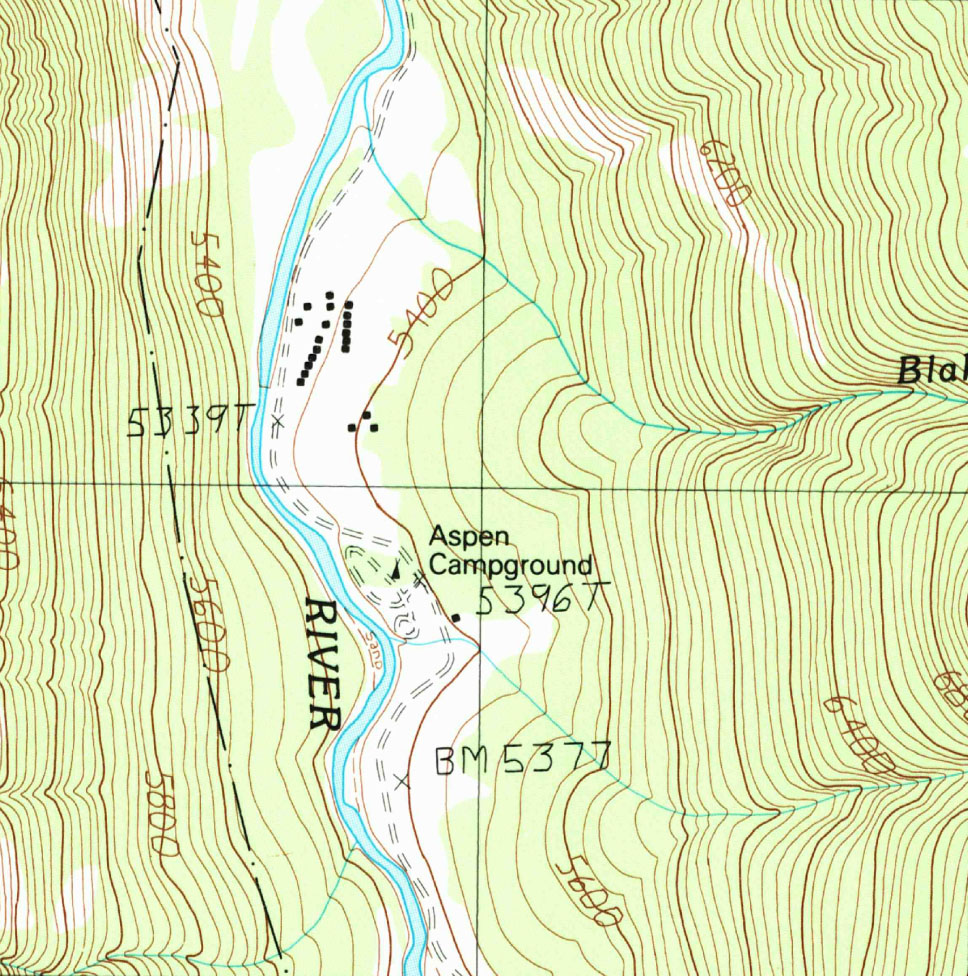
\includegraphics[scale=.65]{figures/MT_ChromeMountain_topo_small.pdf}
%}

Given a function $z=f(x,y)$, we can draw a ``topographical map'' of $f$ by drawing \textbf{level curves} (or, contour lines). A level curve at $z=c$ is a curve in the $x$-$y$ plane such that for all points $(x,y)$ on the curve, $f(x,y) = c$. 

When drawing level curves, it is important that the $c$ values are spaced equally apart as that gives the best insight to how quickly the ``elevation'' is changing. Examples will help one understand this concept.\\

\example{ex_levelcurve1}{Drawing Level Curves}{
Let $\ds f(x,y) = \sqrt{1-\frac{x^2}9-\frac{y^2}4}$. Find the level curves of $f$ for $c=0$, $0.2$, $0.4$, $0.6$, $0.8$ and $1$.}
{Consider first $c=0$. The level curve for $c=0$ is the set of all points $(x,y)$ such that $0=\sqrt{1-\frac{x^2}9-\frac{y^2}4}$. Squaring both sides  gives us
$$\frac{x^2}9+\frac{y^2}4=1,$$ an ellipse centered at $(0,0)$ with horizontal major axis of length 6 and minor axis of length 4. Thus for any point $(x,y)$ on this curve, $f(x,y) = 0$.

Now consider the level curve for $c=0.2$
\begin{align*}
0.2 &= \sqrt{1-\frac{x^2}9-\frac{y^2}4}\\
0.04 &= 1-\frac{x^2}9-\frac{y^2}4\\
\frac{x^2}9+\frac{y^2}4 &=0.96\\
\frac{x^2}{8.64}+\frac{y^2}{3.84} &=1.
\end{align*}
This is also an ellipse, where $a = \sqrt{8.64}\approx 2.94$ and $b=\sqrt{3.84}\approx 1.96$.

In general, for $z=c$, the level curve is:
\begin{align*}
c &= \sqrt{1-\frac{x^2}9-\frac{y^2}4}\\
c^2 &= 1-\frac{x^2}9-\frac{y^2}4\\
\frac{x^2}9+\frac{y^2}4 &=1-c^2\\
\frac{x^2}{9(1-c^2)}+\frac{y^2}{4(1-c^2)} &=1,
\end{align*}
ellipses that are decreasing in size as $c$ increases. A special case is when $c=1$; there the ellipse is just the point $(0,0)$. 

The level curves are shown in Figure \ref{fig:levelcurves1}(a). Note how the level curves for $c=0$ and $c=0.2$ are very, very close together: this indicates that $f$ is growing rapidly along those curves.

\mtable{.67}{Graphing the level curves in Example \ref{ex_levelcurve1}.}{fig:levelcurves1}{%
\begin{tabular}{c}
\myincludegraphics{figures/figlevelcurve1b}\\
(a)\\[10pt]
\myincludegraphicsthree{width=150pt,3Dmenu,activate=onclick,deactivate=pageinvisible,
3Droll=0,
3Dortho=0.004999999888241291,
3Dc2c=0.6562340259552002 0.7273486256599426 0.20080043375492096,
3Dcoo=2.348435640335083 -6.5163373947143555 66.12745666503906,
3Droo=129.99999641808185,
3Dlights=Headlamp,add3Djscript=asylabels.js}{}{figures/figlevelcurve1}\\
%\myincludegraphics[scale=1.25,trim=3mm 0mm 3mm 0mm,clip]{figures/figlevelcurve1}\\
(b)
\end{tabular}
}

In Figure \ref{fig:levelcurves1}(b), the curves are drawn on a graph of $f$ in space. Note how the elevations are evenly spaced. Near the level curves of $c=0$ and $c=0.2$ we can see that $f$ indeed is growing quickly.
}\\

\example{ex_levelcurves2}{Analyzing Level Curves}{
Let $\ds f(x,y) = \frac{x+y}{x^2+y^2+1}$. Find the level curves for $z=c$.}
{We begin by setting $f(x,y)=c$ for an arbitrary $c$ and seeing if algebraic manipulation of the equation reveals anything significant.
\begin{align*}
\frac{x+y}{x^2+y^2+1} &= c \\
x+y &= c(x^2+y^2+1).
\intertext{We recognize this as a circle, though the center and radius are not yet clear. By completing the square, we can obtain:}
\left(x-\frac{1}{2c}\right)^2+\left(y-\frac1{2c}\right)^2&=\frac{1}{2c^2}-1,
\end{align*}
a circle centered at $\big(1/(2c),1/(2c)\big)$ with radius $\sqrt{1/(2c^2)-1}$, where $|c|<1/\sqrt{2}$. The level curves for $c=\pm 0.2,\ \pm 0.4$ and $\pm0.6$ are sketched in Figure \ref{fig:levelcurves2}(a). To help illustrate ``elevation,'' we use thicker lines for $c$ values near 0, and dashed lines indicate where $c<0$. 

There is one special level curve, when $c=0$. The level curve in this situation is $x+y=0$, the line $y=-x$.

In Figure \ref{fig:levelcurves2}(b) we see a graph of the surface. Note how the $y$-axis is pointing away from the viewer to more closely resemble the orientation of the level curves in (a). 

\mtable{.7}{Graphing the level curves in Example \ref{ex_levelcurves2}.}{fig:levelcurves2}{%
\begin{tabular}{c}
\myincludegraphics{figures/figlevelcurve2b}\\
(a)\\[10pt]
%\myincludegraphics[scale=1.2,trim=0mm 5mm 0mm 0mm,clip]{figures/figlevelcurve2}\\
{\myincludegraphicsthree{width=150pt,3Dmenu,activate=onclick,deactivate=pageinvisible,
3Droll=0.25732633644359904,
3Dortho=0.004999999888241291,
3Dc2c=0.5196654200553894 -0.7088789939880371 0.4769051671028137,
3Dcoo=-0.7249413728713989 1.7016432285308838 3.277412176132202,
3Droo=130.00000541214214,
3Dlights=Headlamp,add3Djscript=asylabels.js}{}{figures/figlevelcurve2}}\\
(b)
\end{tabular}
}



%\mfigurethree[width=150pt,3Dmenu,activate=onclick,deactivate=pageinvisible,
%3Droll=0,
%3Dc2c=1 -1.5 1,
%3Dcoo=0 0 0,
%3Droo=130,
%3Dortho=.005,
%3Dlights=Headlamp,add3Djscript=asylabels.js]{.4}{Visualizing the solid shown from Example \ref{ex_doublepol4}.}{fig:doublepol4}{figures/figlevelcurve2_3D} 

Seeing the level curves helps us understand the graph. For instance, the graph does not make it clear that one can ``walk'' along the line $y=-x$ without elevation change, though the level curve does.
}\\

\noindent\textbf{\large Functions of Three Variables}\\

We extend our study of multivariable functions to functions of three variables. (One can make a function of as many variables as one likes; we limit our study to three variables.)

\definition{def:multi3}{Function of Three Variables}
{Let $D$ be a subset of $\mathbb{R}^3$. A \textbf{function $f$ of three variables} is a rule that assigns each triple $(x,y,z)$ in $D$ a value $w=f(x,y,z)$ in $\mathbb{R}$. $D$ is the \textbf{domain} of $f$; the set of all outputs of $f$ is the \textbf{range}.
\index{multivariable function}\index{function!of three variables}\index{multivariable function!domain}\index{multivariable function!range}
}

Note how this definition closely resembles that of Definition \ref{def:multi2}.\\

\example{ex_multi3}{Understanding a function of three variables}{
Let $\ds f(x,y,z) =  \frac{x^2+z+3\sin y}{x+2y-z}.$ Evaluate $f$ at the point $(3,0,2)$ and find the domain and range of $f$.}
{$\ds f(3,0,2) = \frac{3^2+2+3\sin 0}{3+2(0)-2} = 11.$

As the domain of $f$ is not specified, we take it to be the set of all triples $(x,y,z)$ for which $f(x,y,z)$ is defined. As we cannot divide by $0$, we find the domain $D$ is 
$$D = \{(x,y,z)\ |\ x+2y-z\neq 0\}.$$
We recognize that the set of all points in $\mathbb{R}^3$ that \textit{are not} in $D$ form a plane in space that passes through the origin (with normal vector $\la 1,2,-1\ra$). 

We determine the range $R$ is $\mathbb{R}$; that is, all real numbers are possible outputs of $f$. There is no set way of establishing this. Rather, to get numbers near 0 we can let $y=0$ and choose $z \approx -x^2$. To get numbers of arbitrarily large magnitude, we can let $z\approx x+2y$. 
}\\

\clearpage
\noindent\textbf{\large Level Surfaces}\\

It is very difficult to produce a meaningful graph of a function of three variables. A function of \textit{one} variable is a \textit{curve} drawn in \textit{2} dimensions; a function of \textit{two} variables is a \textit{surface} drawn in \textit{3} dimensions; a function of \textit{three} variables is a \textit{hypersurface} drawn in \textit{4} dimensions.\index{multivariable function!level surface}\index{level surface}

There are a few techniques one can employ to try to ``picture'' a graph of three variables. One is an analogue of level curves: \textbf{level surfaces}. Given $w=f(x,y,z)$, the level surface at $w=c$ is the surface in space formed by all points $(x,y,z)$ where $f(x,y,z)=c$. \\

\example{ex_multi4}{Finding level surfaces}{
If a point source $S$ is radiating energy, the intensity $I$ at a given point $P$ in space is inversely proportional to the square of the distance between $S$ and $P$. That is, when $S=(0,0,0)$,  $\ds I(x,y,z) = \frac{k}{x^2+y^2+z^2}$ for some constant $k$.

Let $k=1$; find the level surfaces of $I$.}
{We can (mostly) answer this question using ``common sense.'' If energy (say, in the form of light) is emanating from the origin, its intensity will be the same at all points equidistant from the origin. That is, at any point on the surface of a sphere centered at the origin, the intensity should be the same. Therefore, the level surfaces are spheres.

We now find this mathematically. The level surface at $I=c$ is defined by 
\begin{align*}
c &= \frac{1}{x^2+y^2+z^2}.
\intertext{A small amount of algebra reveals}
x^2+y^2+z^2 &= \frac1c.
\end{align*}
Given an intensity $c$, the level surface $I=c$ is a sphere of radius $1/\sqrt{c}$, centered at the origin. 

\mtable{.4}{A table of $c$ values and the corresponding radius $r$ of the spheres of constant value in Example \ref{ex_multi4}.}{fig:multi4}{
\begin{tabular}{cc}
$c$ & $r$ \\ \hline
16. & 0.25 \\
 8. & 0.35 \\
 4. & 0.5 \\
 2. & 0.71 \\
 1. & 1. \\
 0.5 & 1.41 \\
 0.25 & 2. \\
 0.125 & 2.83 \\
 0.0625 & 4. \\
\end{tabular}
}

Figure \ref{fig:multi4} gives a table of the radii of the spheres for given $c$ values. Normally one would use equally spaced $c$ values, but these values have been chosen purposefully. At a distance of 0.25 from the point source, the intensity is 16; to move to a point of half that intensity, one just moves out 0.1 to 0.35 -- not much at all. To again halve the intensity, one moves 0.15, a little more than before.

Note how each time the intensity if halved, the distance required to move away grows. We conclude that the closer one is to the source, the more rapidly the intensity changes.
}\\

\enlargethispage{2\baselineskip}
In the next section we apply the concepts of limits to functions of two or more variables.

\printexercises{exercises/12_01_exercises}
%\section{Limits and Continuity of Multivariable Functions}\label{sec:multi_limit}

We continue with the pattern we have established in this text: after defining a new kind of function, we apply calculus ideas to it. The previous section defined functions of two and three variables; this section investigates what it means for these functions to be ``continuous.''

We begin with a series of definitions. We are used to ``open intervals'' such as $(1,3)$, which represents the set of all $x$ such that $1<x<3$,  and ``closed intervals'' such as $[1,3]$, which represents the set of all $x$ such that $1\leq x\leq 3$. We need analogous definitions for open and closed sets in the $x$-$y$ plane.

\definition{def:open}{\parbox[t]{180pt}{Open Disk, Boundary and Interior Points, Open and Closed Sets, Bounded Sets}}
{An \textbf{open disk} $B$ in $\mathbb{R}^2$ centered at $(x_0,y_0)$ with radius $r$ is the set of all points $(x,y)$ such that $\ds\sqrt{(x-x_0)^2+(y-y_0)^2} < r$. \\

Let $S$ be a set of points in $\mathbb{R}^2$. A point $P$ in $\mathbb{R}^2$ is a \textbf{boundary point} of $S$  if all open disks centered at $P$ contain both points in $S$ and points not in $S$.\\

A point $P$ in $S$ is an \textbf{interior point} of $S$ if there is an open disk centered at $P$ that contains only points in $S$. \\

A set $S$ is \textbf{open} if every point in $S$ is an interior point.\\

A set $S$ is \textbf{closed} if it contains all of its boundary points.\\

A set $S$ is \textbf{bounded} if there is an $M>0$ such that the open disk, centered at the origin with radius $M$, contains $S$. A set that is not bounded is \textbf{unbounded}.
\index{open}\index{closed}\index{open disk}\index{closed disk}\index{boundary point}\index{interior point}\index{bounded set}\index{unbounded set}
}

Figure \ref{fig:multilimit_intro} shows several sets in the $x$-$y$ plane. In each set, point $P_1$ lies on the boundary of the set as all open disks centered there contain both points in, and not in, the set. In contrast, point $P_2$ is an interior point for there is an open disk centered there that lies entirely within the set.
\mtable{.6}{Illustrating open and closed sets in the $x$-$y$ plane.}{fig:multilimit_intro}{%
\begin{tabular}{c}
\myincludegraphics{figures/figmultilimit_introa}\\
(a)\\[10pt]
\myincludegraphics{figures/figmultilimit_introb}\\
(b)\\[10pt]
\myincludegraphics{figures/figmultilimit_introc}\\
(c)\\[10pt]
\end{tabular}
}

The set depicted in Figure \ref{fig:multilimit_intro}(a) is a closed set as it contains all of its boundary points. The set in (b) is open, for all of its points are interior points (or, equivalently, it does not contain any of its boundary points). The set in (c) is neither open nor closed as it contains  some of its boundary points.\\
\clearpage

\example{ex_multilimit1}{Determining open/closed, bounded/unbounded}{
Determine if the domain of the function $f(x,y)=\sqrt{1-x^2/9-y^2/4}$ is open, closed, or neither, and if it is bounded.}
{This domain of this function was found in Example \ref{ex_multi2} to be $D = \{(x,y)\ |\ \frac{x^2}9+\frac{y^2}4\leq 1\}$, the region \textit{bounded} by the ellipse $\frac{x^2}9+\frac{y^2}4=1$. Since the region includes the boundary (indicated by the use of ``$\leq$''), the set contains all of its boundary points and hence is closed. The region is bounded as a disk of radius 4, centered at the origin, contains $D$.
}\\

\example{ex_multilimit2}{Determining open/closed, bounded/unbounded}{
Determine if the domain of $f(x,y) = \frac1{x-y}$ is open, closed, or neither.}
{As we cannot divide by 0, we find the domain to be $D = \{(x,y)\ |\ x-y\neq 0\}$. In other words, the domain is the set of all points $(x,y)$ \emph{not} on the line $y=x$. 

\mfigure{.63}{Sketching the domain of the function in Example \ref{ex_multilimit2}.}{fig:multilimit2}{figures/figmultilimit2}
The domain is sketched in Figure \ref{fig:multilimit2}. Note how we can draw an open disk around any point in the domain that lies entirely inside the domain, and also note how the only boundary points of the domain are the points on the line $y=x$. We conclude the domain is an open set. The set is unbounded.
}\\

\noindent\textbf{\large Limits}\\

Recall a pseudo--definition of the limit of a function of one variable: ``$\ds \lim_{x\to c}f(x) = L$'' means that if $x$ is ``really close'' to $c$, then $f(x)$ is ``really close'' to $L$. A similar pseudo--definition holds for functions of two variables. We'll say that 
\enlargethispage{3\baselineskip}

\begin{center}
``$\ds \lim_{(x,y)\to (x_0,y_0)} f(x,y) = L$'' \end{center}
means ``if the point $(x,y)$ is really close to the point $(x_0,y_0)$, then $f(x,y)$ is really close to $L$.'' The formal definition is given below.
\mnote{.33}{\textbf{Note:} %As sets in the plane can be more complicated than simple intervals along the real line, Definition \ref{def:multilimita} contain language about the shape of a set $S$ that is different from our first limit definition. %
While our first limit definition was defined over an open interval, we now define limits over a set $S$ in the plane (where $S$ does not have to be open). As planar sets can be far more complicated than intervals, our definition adds the restriction ``$\ldots$ where every open disk centered at $P$ contains points in $S$ other than $P$.'' 
In this text, all sets we'll consider will satisfy this condition and we won't bother to check; it is included in the definition for completeness.}

%\setboxwidth{40pt}
\definition{def:multilimita}{Limit of a Function of Two Variables}
{Let $S$ be a set containing $P=(x_0,y_0)$ where every open disk centered at $P$ contains points in $S$ other than $P$, let $f$ be a function of two variables defined on $S$, except possibly at $P$, and let $L$ be a real number. 
%Let $f(x,y)$ be a function of two variables and let $(x_0,y_0)$ be a point in the domain of $f$. 
The \sword{limit of $f(x,y)$ as $(x,y)$ approaches $(x_0,y_0)$ is $L$}, denoted $$\ds \lim_{(x,y)\to (x_0,y_0)} f(x,y) = L,$$
means that given any $\epsilon>0$, there exists $\delta>0$ such that for all  $(x,y)$ in $S$, where $(x,y)\neq (x_0,y_0)$, if $(x,y)$ is in the open disk centered at $(x_0,y_0)$ with radius $\delta$, then $|f(x,y) - L|<\epsilon.$
\index{limit!of multivariable function}\index{multivariable function!limit}
}
%\definition{def:multilimit}{Limit of a Function of Two Variables}
%{Let $S$ be an open set containing $(x_0,y_0)$, and let $f$ be a function of two variables defined on $S$, except possibly at $(x_0,y_0)$. 
%%Let $f(x,y)$ be a function of two variables and let $(x_0,y_0)$ be a point in the domain of $f$. 
%The \textbf{limit} of $f(x,y)$ as $(x,y)$ approaches $(x_0,y_0)$ is $L$, denoted $$\ds \lim_{(x,y)\to (x_0,y_0)} f(x,y) = L,$$
%means that given any $\epsilon>0$, there exists $\delta>0$ such that for all  $(x,y)\neq (x_0,y_0)$, if $(x,y)$ is in the open disk centered at $(x_0,y_0)$ with radius $\delta$, then $|f(x,y) - L|<\epsilon.$
%\index{limit!of multivariable function}\index{multivariable function!limit}
%}


The concept behind Definition \ref{def:multilimit} is sketched in Figure \ref{fig:multilimitdef}. Given $\epsilon>0$, find $\delta>0$ such that if $(x,y)$ is any point in the open disk centered at $(x_0,y_0)$ in the $x$-$y$ plane with radius $\delta$, then $f(x,y)$ should be within $\epsilon$ of $L$. 

\enlargethispage{1\baselineskip}
Computing limits using this definition is rather cumbersome. The following theorem allows us to evaluate limits much more easily.

\mfigurethree{width=150pt,3Dmenu,activate=onclick,deactivate=onclick,
3Droll=0.12234160136132792,
3Dortho=0.004824123345315456,
3Dc2c=0.9118747115135193 -0.1974218785762787 0.35987377166748047,
3Dcoo=21.82058334350586 66.31769561767578 47.81545639038086,
3Droo=149.99999973566392,
3Dlights=Headlamp,add3Djscript=asylabels.js}{scale=1.25}{.77}{\textbf{Illustrating the definition of a limit.} The open disk in the $x$-$y$ plane has radius $\delta$. Let $(x,y)$ be any point in this disk; $f(x,y)$ is within $\epsilon$ of $L$.}{fig:multilimitdef}{figures/figmultilimit_def}
%\mfigure[scale=1.25]{.77}{\textbf{Illustrating the definition of a limit.} The open disk in the $x$-$y$ plane has radius $\delta$. Let $(x,y)$ be any point in this disk; $f(x,y)$ is within $\epsilon$ of $L$.}{fig:multilimitdef}{figures/figmultilimit_def}


%\setboxwidth{0pt}
\theorem{thm:multi_limit_algebra}{\parbox[t]{180pt}{Basic Limit Properties of Functions of Two Variables}}{%\small
Let $b$, $x_0$, $y_0$, $L$ and $K$ be real numbers,  let $n$ be a positive integer, and let $f$ and $g$ be functions with the following limits:
$$\lim_{(x,y)\to (x_0,y_0)}f(x,y) = L \quad \text{\ and\ } \lim_{(x,y)\to (x_0,y_0)} g(x,y) = K.$$
The following limits hold.
\index{limit!of multivariable function}\index{limit!properties}\index{multivariable function!limit}
\begin{enumerate}
\item \parbox{80pt}{Constants:} $\displaystyle \lim_{(x,y)\to (x_0,y_0)} b = b$
\item	\parbox{80pt}{Identity }	$\displaystyle \lim_{(x,y)\to (x_0,y_0)} x = x_0$;\qquad $\displaystyle \lim_{(x,y)\to (x_0,y_0)} y = y_0$
\item	\parbox{80pt}{Sums/Differences:} $\displaystyle \lim_{(x,y)\to (x_0,y_0)}\big(f(x,y)\pm g(x,y)\big) = L\pm K$
\item	\parbox{80pt}{Scalar Multiples:}	$\displaystyle \lim_{(x,y)\to (x_0,y_0)} b\cdot f(x,y) = bL$
\item	\parbox{80pt}{Products:}	$\displaystyle \lim_{(x,y)\to (x_0,y_0)} f(x,y)\cdot g(x,y) = LK$
\item	\parbox{80pt}{Quotients:} $\displaystyle \lim_{(x,y)\to (x_0,y_0)} f(x,y)/g(x,y) = L/K$, ($K\neq 0)$
\item	\parbox{80pt}{Powers:} 	$\displaystyle \lim_{(x,y)\to (x_0,y_0)} f(x,y)^n = L^n$
%\item	\parbox{80pt}{Roots:}		\parbox[t]{185pt}{$\displaystyle \lim_{(x,y)\to (x_0,y_0)} \sqrt[n]{f(x,y)} = \sqrt[n]{L}$}% \qquad \small (if $n$ is even then $L$ must be greater than 0; when $n$ is odd, it is true for all $L$.)}

\end{enumerate}
}
\restoreboxwidth

This theorem, combined with Theorems \ref{thm:poly_rat} and \ref{thm:lim_continuous} of Section \ref{sec:limit_analytically}, allows us to evaluate many limits.\\

\example{ex_multilimit3}{Evaluating a limit}{
Evaluate the following limits:
$$1. \lim_{(x,y)\to (1,\pi)} \frac yx + \cos(xy) \qquad\qquad 2. \lim_{(x,y)\to (0,0)} \frac{3xy}{x^2+y^2}$$
}
{\begin{enumerate}
	\item The aforementioned theorems allow us to simply evaluate $y/x+\cos(xy)$ when $x=1$ and $y=\pi$. If an indeterminate form is returned, we must do more work to evaluate the limit; otherwise, the result is the limit. Therefore
	\begin{align*}
	\lim_{(x,y)\to (1,\pi)} \frac yx + \cos(xy)  &= \frac\pi{1}+\cos \pi \\
		&= \pi -1.
	\end{align*}
	\item		We attempt to evaluate the limit by substituting 0 in for $x$ and $y$, but the result is the indeterminate form ``$0/0$.'' To evaluate this limit, we must ``do more work,'' but we have not yet learned what ``kind'' of work to do. Therefore we cannot yet evaluate this limit.
\end{enumerate}
\vskip -1.5\baselineskip
}\\

When dealing with functions of a single variable we also considered one--sided limits and stated
$$\lim_{x\to c}f(x) = L \quad\text{ if, and only if,}\quad \lim_{x\to c^+}f(x) =L \quad\textbf{ and}\quad \lim_{x\to c^-}f(x) =L.$$
That is, the limit is $L$ if and only if $f(x)$ approaches $L$ when $x$ approaches $c$ from \textbf{either} direction, the left or the right.

In the plane, there are infinite directions from which $(x,y)$ might approach $(x_0,y_0)$. In fact, we do not have to restrict ourselves to approaching $(x_0,y_0)$ from a particular direction, but rather we can approach that point along a path that is not a straight line. It is possible to arrive at different limiting values by approaching $(x_0,y_0)$ along different paths. If this happens, we say that $\ds \lim_{(x,y)\to(x_0,y_0) } f(x,y)$ does not exist (this is analogous to the left and right hand limits of single variable functions not being equal).

Our theorems tell us that we can evaluate most limits quite simply, without worrying about  paths. When indeterminate forms arise, the limit may or may not exist. If it does exist, it can be difficult to prove this as we need to show the same limiting value is obtained regardless of the path chosen. The case where the limit does not exist is often easier to deal with, for we can often pick two paths along which the limit is different.\\

%it can be difficult to show that the limit exists, for we need to show that the same limiting value is obtained regardless of the path taken.  we can often evaluate the limit along specific paths. If any of these limits differ, we say that \emph{the} limit does not exist.\\

\example{ex_multilimit4}{Showing limits do not exist}{
\begin{enumerate}
	\item Show $\ds \lim_{(x,y)\to (0,0)} \frac{3xy}{x^2+y^2}$ does not exist by finding the limits along the lines $y=mx$.
	\item	Show $\ds \lim_{(x,y)\to (0,0)} \frac{\sin(xy)}{x+y}$ does not exist by finding the limit along the path $y=-\sin x$. 	
\end{enumerate}
}
{\begin{enumerate}
	\item Evaluating $\ds \lim_{(x,y)\to (0,0)} \frac{3xy}{x^2+y^2}$ along the lines $y=mx$ means replace all $y$'s with $mx$ and evaluating the resulting limit:
	\begin{align*}
	\lim_{(x,mx)\to (0,0)} \frac{3x(mx)}{x^2+(mx)^2} &=\lim_{x\to 0} \frac{3mx^2}{x^2(m^2+1)}\\
				&= \lim_{x\to 0} \frac{3m}{m^2+1}\\
				&= \frac{3m}{m^2+1}.
	\end{align*}
	While the limit exists for each choice of $m$, we get a \emph{different} limit for each choice of $m$. That is, along different lines we get differing limiting values, meaning \emph{the} limit does not exist.
	
	\item		Let $f(x,y) = \frac{\sin(xy)}{x+y}$. We are to show that $\ds \lim_{(x,y)\to (0,0)} f(x,y)$ does not exist by finding the limit along the path $y=-\sin x$. First, however, consider the limits found along the lines $y=mx$ as done above.
	\begin{align*}
	\lim_{(x,mx)\to (0,0)} \frac{\sin\big(x(mx)\big)}{x+mx} &= \lim_{x\to 0} \frac{\sin (mx^2)}{x(m+1)} \\
	&= \lim_{x\to 0} \frac{\sin(mx^2)}{x}\cdot\frac1{m+1}.
	\end{align*}
	By applying L'H\^opital's Rule, we can show this limit is 0 \emph{except} when $m=-1$, that is, along the line $y=-x$. This line is not in the domain of $f$, so we have found the following fact: along every line $y=mx$ in the domain of $f$, $\ds \lim_{(x,y)\to(0,0)} f(x,y)=0$. %Along this line, $f(x,y)$ is not defined, so it stands to reason that a limit along this line does not exist.
\drawexampleline
	
	Now consider the limit along the path $y=-\sin x$:
	\begin{align*}
	\lim_{(x,-\sin x)\to (0,0)} \frac{\sin\big(-x\sin x\big)}{x-\sin x} &= \lim_{x\to0} \frac{\sin\big(-x\sin x\big)}{x-\sin x}
	\end{align*}
	Now apply L'H\^opital's Rule twice:
	\small
	\begin{align*}
	 \quad &= \lim_{x\to 0}\frac{\cos\big(-x\sin x\big)(-\sin x-x\cos x)}{1-\cos x} \quad \left(\text{``}= 0/0\text{''}\right)\\
	&= \lim_{x\to 0}\frac{-\sin\big(-x\sin x\big)(-\sin x-x\cos x)^2+\cos\big(-x\sin x\big)(-2\cos x+x\sin x)}{\sin x}\\
	&= \text{``$-2/0$''} \Rightarrow \text{the limit does not exist.}
	\end{align*}
	\normalsize
Step back and consider what we have just discovered. Along any line $y=mx$ in the domain of the $f(x,y)$, the limit is 0. However, along the path $y=-\sin x$, which lies in the domain of  $f(x,y)$ for all $x\neq 0$, the limit does not exist. Since the limit is not the same along every path to $(0,0)$, we say $\ds \lim_{(x,y)\to (0,0)}\frac{\sin(xy)}{x+y}$ does not exist.
\end{enumerate}
\vskip -1.5\baselineskip
}\\

\example{ex_multilimit5}{Finding a limit}{
Let $\ds f(x,y) = \frac{5x^2y^2}{x^2+y^2}$. Find $\ds\lim_{(x,y)\to (0,0)}  f(x,y) .$
}
{It is relatively easy to show that along any line $y=mx$, the limit is 0. This is not enough to prove that the limit exists, as demonstrated in the previous example, but it tells us that if the limit does exist then it must be 0.

To prove the limit is 0, we apply Definition \ref{def:multilimit}. Let $\epsilon >0$ be given. We want to find $\delta >0$ such that if $\sqrt{(x-0)^2+(y-0)^2} <\delta$, then $|f(x,y)-0| <\epsilon$.

Set $\delta < \sqrt{\epsilon/5}$. Note that $\ds \left|\frac{5y^2}{x^2+y^2}\right| <5$ for all $(x,y)\neq (0,0)$, and that if $\sqrt{x^2+y^2} <\delta$, then $x^2<\delta^2$.

Let $\sqrt{(x-0)^2+(y-0)^2} = \sqrt{x^2+y^2}<\delta$. Consider $|f(x,y)-0|$:
\begin{align*}
|f(x,y)-0| &= \left|\frac{5x^2y^2}{x^2+y^2}-0\right| \\
				&= \left|x^2\cdot\frac{5y^2}{x^2+y^2}\right|\\
				&< \delta^2\cdot 5 \\
				&< \frac{\epsilon}{5}\cdot 5 \\
				&= \epsilon.
\end{align*}
Thus if $\sqrt{(x-0)^2+(y-0)^2}<\delta$ then $|f(x,y)-0|<\epsilon$, which is what we wanted to show. Thus $\ds \lim_{(x,y)\to(0,0)} \frac{5x^2y^2}{x^2+y^2} = 0$.
}\\

\noindent\textbf{\large Continuity}\\

Definition \ref{def:continuous} defines what it means for a function of one variable to be continuous. In brief, it meant that the graph of the function did not have breaks, holes, jumps, etc. We define continuity for functions of two variables in a similar way as we did for functions of one variable.

\definition{def:multi_continuous}{Continuous}
{Let a function $f(x,y)$ be defined on a set $S$ containing the point $(x_0,y_0)$. 

\begin{enumerate}
	\item $f$ is \textbf{continuous} at $(x_0,y_0)$ if $\ds\lim_{(x,y)\to(x_0,y_0)} f(x,y) = f(x_0,y_0)$.
	\index{continuous function}\index{multivariable function!continuity}
	\item	$f$ is \textbf{continuous on $S$} if $f$ is continuous at all points in $S$. If $f$ is continuous at all points in $\mathbb{R}^2$, we say that $f$ is \textbf{continuous everywhere}.
\end{enumerate}
}

\example{ex_multicont1}{Continuity of a function of two variables}{
Let $\ds f(x,y) = \left\{ \begin{array}{rl} \frac{\cos y\sin x}{x} & x\neq 0 \\
																						\cos y & x=0
													\end{array} \right.$. Is $f$ continuous at $(0,0)$? Is $f$ continuous everywhere?
}
{To determine if $f$ is continuous at $(0,0)$, we need to compare $\ds\lim_{(x,y)\to (0,0)} f(x,y)$ to $f(0,0)$. 

Applying the definition of $f$, we see that $f(0,0) = \cos 0 = 1$. 

We now consider the limit $\ds \lim_{(x,y)\to (0,0)} f(x,y)$. Substituting $0$ for $x$ and $y$ in $(\cos y\sin x)/x$ returns the indeterminate form ``0/0'', so we need to do more work to evaluate this limit.

Consider two related limits: $\ds \lim_{(x,y)\to (0,0)} \cos y$ and $\ds \lim_{(x,y)\to(0,0)} \frac{\sin x}x$. The first limit does not contain $x$, and since $\cos y$ is continuous, $$\ds \lim_{(x,y)\to (0,0)} \cos y =\lim_{y\to 0} \cos y = \cos 0 = 1.$$

The second limit does not contain $y$. By Theorem \ref{thm:special_limits} we can say
$$\lim_{(x,y)\to (0,0)} \frac{\sin x}{x} = \lim_{x\to 0} \frac{\sin x}{x} = 1.$$
Finally, Theorem \ref{thm:multi_limit_algebra} of this section states that we can combine these two limits as follows:
\begin{align*}
\lim_{(x,y)\to (0,0)} \frac{\cos y\sin x}{x} &= \lim_{(x,y)\to (0,0)} (\cos y)\left(\frac{\sin x}{x}\right) \\ 
&=\left(\lim_{(x,y)\to (0,0)} \cos y\right)\left(\lim_{(x,y)\to (0,0)} \frac{\sin x}{x}\right) \\
  &= (1)(1)\\
	&=1.
\end{align*}

We have found that $\ds \lim_{(x,y)\to (0,0)} \frac{\cos y\sin x}{x} = f(0,0)$, so $f$ is continuous at $(0,0)$.

A similar analysis shows that $f$ is continuous at all points in $\mathbb{R}^2$. As long as $x\neq0$, we can evaluate the limit directly; when $x=0$, a similar analysis shows that the limit is $\cos y$. Thus we can say that $f$ is continuous everywhere. A graph of $f$ is given in Figure \ref{fig:multicont1}. Notice how it has no breaks, jumps, etc.
\mfigurethree{width=150pt,3Dmenu,activate=onclick,deactivate=onclick,
3Droll=1.3976649182325884,
3Dortho=0.005226649809628725,
3Dc2c=0.6559564471244812 0.554935097694397 0.5116328597068787,
3Dcoo=-1.2457355260849 0.0923926830291748 4.189182281494141,
3Droo=129.99999868169073,
3Dlights=Headlamp,add3Djscript=asylabels.js}{scale=1.25}{.8}{A graph of $f(x,y)$ in Example \ref{ex_multicont1}.}{fig:multicont1}{figures/figmulticont1}
%\mfigure[scale=1.25]{.8}{A graph of $f(x,y)$ in Example \ref{ex_multicont1}.}{fig:multicont1}{figures/figmulticont1}
}\\

The following theorem is very similar to Theorem \ref{thm:continuity_algebra}, giving us ways to combine continuous functions to create other continuous functions.

\theorem{thm:multi_continuous_prop}{Properties of Continuous Functions}
{Let $f$ and $g$ be continuous on a set $S$, let $c$ be a real number, and let $n$ be a positive integer. The following functions are continuous on $S$.
\index{continuous function!properties}\index{multivariable function!continuity}
		\begin{enumerate}
		\item		\parbox{80pt}{Sums/Differences:}	$f\pm g$
		\item		\parbox{80pt}{Constant Multiples:}	$c\cdot f$
		\item		\parbox{80pt}{Products:}	$f\cdot g$
		\item		\parbox{80pt}{Quotients:}	$f/g$ \qquad {\small (as longs as $g\neq 0$ on $S$)}
		\item		\parbox{80pt}{Powers:}	$f\,^n$
		\item		\parbox{80pt}{Roots:}	$\sqrt[n]{f}$ \qquad \parbox[t]{150pt}{\small (if $n$ is even then $f\geq 0$ on $S$; if $n$ is odd, then true for all values of $f$ on $S$.)}
		\item		\parbox{80pt}{Compositions:}\parbox[t]{185pt}{Adjust the definitions of $f$ and $g$ to: Let $f$ be continuous on $S$, where the range of $f$ on $S$ is $J$, and let $g$ be a single variable function that is continuous on $J$. Then $g\circ f$, i.e., $g(f(x,y))$, is continuous on $S$.}
		\end{enumerate}
}
\enlargethispage{\baselineskip}

\example{ex_multicont2}{Establishing continuity of a function}{
Let $f(x,y) = \sin (x^2\cos y)$. Show $f$ is continuous everywhere.}
{We will apply both Theorems \ref{thm:continuity_algebra} and \ref{thm:multi_continuous_prop}. Let $f_1(x,y) = x^2$. Since $y$ is not actually used in the function, and polynomials are continuous (by Theorem \ref{thm:continuity_algebra}), we conclude $f_1$ is continuous everywhere. A similar statement can be made about $f_2(x,y) = \cos y$. Part 3 of Theorem \ref{thm:multi_continuous_prop} states that $f_3=f_1\cdot f_2$ is continuous everywhere, and Part 7 of the theorem states the composition of sine with $f_3$ is continuous: that is, $\sin (f_3) = \sin(x^2\cos y)$ is continuous everywhere.
}\\

\noindent\textbf{\large Functions of Three Variables}\\

The definitions and theorems given in this section can be extended in a natural way to definitions and theorems about functions of three (or more) variables. We cover the key concepts here; some terms from Definitions \ref{def:open} and \ref{def:multi_continuous} are not redefined but their analogous meanings should be clear to the reader.

\setboxwidth{20pt}
\definition{def:multi3defs}{Open Balls, Limit, Continuous}
{ 
\begin{enumerate}
\item An \textbf{open ball} in $\mathbb{R}^3$ centered at $(x_0,y_0,z_0)$ with radius $r$ is the set of all points $(x,y,z)$ such that $\sqrt{(x-x_0)^2+(y-y_0)^2+(z-z_0)^2} = r$.
\index{multivariable function!limit}\index{limit!of multivariable function}\index{multivariable function!continuity}\index{open ball}
\\

\item Let $D$ be a set in $\mathbb{R}^3$ containing $(x_0,y_0,z_0)$ where every open ball centered at $(x_0,y_0,z_0)$ contains points of $D$ other than $(x_0,y_0,z_0)$, and let $f(x,y,z)$ be a function of three variables defined on $D$, except possibly at  $(x_0,y_0,z_0)$. The \textbf{limit} of $f(x,y,z)$ as $(x,y,z)$ approaches $(x_0,y_0,z_0)$ is $L$, denoted 
$$\lim_{(x,y,z)\to (x_0,y_0,z_0)} f(x,y,z) = L,$$
means that given any $\epsilon >0$, there is a $\delta >0$ such that for all  $(x,y,z)$ in $D$, $(x,y,z)\neq(x_0,y_0,z_0)$, if $(x,y,z)$ is in the open ball centered at $(x_0,y_0,z_0)$ with radius $\delta$, then $|f(x,y,z) - L|< \epsilon$.\\

\item Let $f(x,y,z)$ be defined on a set $D$ containing $(x_0,y_0,z_0)$. $f$ is \textbf{continuous} at $(x_0,y_0,z_0)$ if $\ds \lim_{(x,y,z)\to (x_0,y_0,z_0)} f(x,y,z) = f(x_0,y_0,z_0)$; if $f$ is continuous at all points in $D$, we say $f$ is \sword{continuous on $D$}.
\end{enumerate}
}
\restoreboxwidth

These definitions can also be extended naturally to apply to functions of four or more variables. Theorem \ref{thm:multi_continuous_prop} also applies to function of three or more variables, allowing us to say that the function $$\ds f(x,y,z) = \frac{e^{x^2+y}\sqrt{y^2+z^2+3}}{\sin (xyz)+5}$$ is continuous everywhere.

When considering single variable functions, we studied limits, then continuity, then the derivative. In our current study of multivariable functions, we have studied limits and continuity. In the next section we study derivation, which takes on a slight twist as we are in a multivarible context.

\printexercises{exercises/12_02_exercises}
%\section{Partial Derivatives}\label{sec:partial_derivatives}

Let $y$ be a function of $x$. We have studied in great detail the derivative of $y$ with respect to $x$, that is, $\frac{dy}{dx}$, which measures the rate at which $y$ changes with respect to $x$. Consider now $z=f(x,y)$. It makes sense to want to know how $z$ changes with respect to $x$ and/or $y$. This section begins our investigation into these rates of change.

Consider the function $z=f(x,y) = x^2+2y^2$, as graphed in Figure \ref{fig:partialintro}(a). By fixing $y=2$, we focus our attention to all points on the surface where the $y$-value is 2, shown in both parts (a) and (b) of the figure. These points form a curve in space: $z = f(x,2) = x^2+8$ which is a function of just one variable. We can take the derivative of $z$ with respect to $x$ along this curve and find equations of tangent lines, etc. 

\mtable{.68}{By fixing $y=2$, the surface $f(x,y) = x^2+2y^2$ is a curve in space.}{fig:partialintro}
{\begin{tabular}{c}
\myincludegraphicsthree{width=125pt,3Dmenu,activate=onclick,deactivate=onclick,
3Droll=1.320775024146522,
3Dortho=0.004999999888241291,
3Dc2c=0.6570873856544495 0.6839641332626343 0.31690558791160583,
3Dcoo=-3.0739071369171143 -0.40104401111602783 58.57058334350586,
3Droo=129.99999696026478,
3Dlights=Headlamp,add3Djscript=asylabels.js}{scale=1.25,trim = 2mm 2mm 2mm 2mm,clip}{figures/figpartialintro}\\[10pt]
%\myincludegraphics[scale=1.25,trim = 2mm 2mm 2mm 2mm,clip]{figures/figpartialintro}\\[10pt]
(a)\\[5pt]
\myincludegraphicsthree{width=125pt,3Dmenu,activate=onclick,deactivate=onclick,
3Droll=1.320775024146522,
3Dortho=0.004999999888241291,
3Dc2c=0.6570873856544495 0.6839641332626343 0.31690558791160583,
3Dcoo=-3.0739071369171143 -0.40104401111602783 58.57058334350586,
3Droo=129.99999696026478,
3Dlights=Headlamp,add3Djscript=asylabels.js}{scale=1.25,trim = 2mm 2mm 2mm 2mm,clip}{figures/figpartialintrob}
%\myincludegraphics[scale=1.25,trim = 2mm 2mm 2mm 2mm,clip]{figures/figpartialintrob}\\[10pt]
(b)
\end{tabular}
}

The key notion to extract from this example is: by treating $y$ as  constant (it does not vary) we can consider how $z$ changes with respect to $x$. In a similar fashion, we can hold $x$ constant and consider how $z$ changes with respect to $y$. This is the underlying principle of \textbf{partial derivatives}. We state the formal, limit--based definition first, then show how to compute these partial derivatives without directly taking limits.

%\enlargethispage{4\baselineskip}
\definition{def:partial_derivative}{Partial Derivative}
{Let $z=f(x,y)$ be a continuous function on an open set $S$ in $\mathbb{R}^2$.
\begin{enumerate}
	\item The \textbf{partial derivative of $f$ with respect to $x$} is:
	$$f_x(x,y) = \lim_{h\to 0} \frac{f(x+h,y) - f(x,y)}h.$$
	%Alternate notations for $\frac{\partial z}{\partial x}$ include: $\ds\frac{\partial}{\partial x}f(x,y),\ f_x(x,y),\ \text{and}\ z_x.$
	\item The \textbf{partial derivative of $f$ with respect to $y$} is:
	$$f_y(x,y) = \lim_{h\to 0} \frac{f(x,y+h) - f(x,y)}h.$$
	
	%\item		If $f_x$ and $f_y$ are continuous on $S$, then $f$ is \textbf{differentiable} on $S$.\footnote{This definition of differentiability is mathematically ``weak'' but easy to understand; see Section \ref{sec:total_differential} for a stronger definition that is less intuitive.}
	\end{enumerate}
	\index{partial derivative}\index{derivative!partial}
}
\mnote{.35}{Alternate notations for $f_x(x,y)$ include: $$\frac{\partial}{\partial x}f(x,y),\ \ \frac{\pf}{\px},\ \ \frac{\pz}{\px},\ \ \text{and}\ z_x,$$ with similar notations for $f_y(x,y).$ For ease of notation, $f_x(x,y)$ is often abbreviated $f_x$.}

\example{ex_partial1}{Computing partial derivatives with the limit definition}{
Let $f(x,y) = x^2y + 2x+y^3$. Find $f_x(x,y)$ using the limit definition.}
{Using Definition \ref{def:partial_derivative}, we have:
\begin{align*}
f_x(x,y) &= \lim_{h\to 0} \frac{f(x+h,y) - f(x,y)}{h} \\
				&= \lim_{h\to 0} \frac{(x+h)^2y+2(x+h)+y^3 - (x^2y+2x+y^3)}{h}\\
				&= \lim_{h\to 0} \frac{x^2y+2xhy+h^2y+2x+2h+y^3-(x^2y+2x+y^3)}{h}\\
				&= \lim_{h\to 0} \frac{2xhy+h^2y+2h}{h}\\
				&=\lim_{h\to 0} 2xy+hy+2\\
				&= 2xy+2.
\end{align*}
We have found $f_x(x,y) = 2xy+2$.
}\\

Example \ref{ex_partial1} found a partial derivative using the formal, limit--based definition. Using limits is not necessary, though, as we can rely on our previous knowledge of derivatives to compute partial derivatives easily. When computing $f_x(x,y)$, we hold $y$ fixed -- it does not vary. Therefore we can compute the derivative with respect to $x$ by treating $y$ as a constant or coefficient. 

Just as $\frac{d}{dx}\big(5x^2\big) = 10x$, we compute $\frac{\partial}{\px}\big(x^2y\big) = 2xy$. Here we are treating $y$ as a coefficient.

Just as $\frac{d}{dx}\big(5^3\big) = 0$, we compute $\frac{\partial}{\px}\big(y^3\big) = 0.$ Here we are treating $y$ as a constant. More examples will help make this clear.\\

\example{ex_partial2}{Finding partial derivatives}{
Find $f_x(x,y)$ and $f_y(x,y)$ in each of the following.
\begin{enumerate}
	\item $f(x,y) = x^3y^2+ 5y^2-x+7$
	\item	$f(x,y) = \cos(xy^2)+\sin x$
	\item	$f(x,y) = e^{x^2y^3}\sqrt{x^2+1}$
\end{enumerate} 
}
{\begin{enumerate}
	\item We have $f(x,y) = x^3y^2+ 5y^2-x+7$.\\
	Begin with $f_x(x,y)$. Keep $y$ fixed, treating it as a constant or coefficient, as appropriate:
	$$f_x(x,y) = 3x^2y^2-1.$$ Note how the $5y^2$ and $7$ terms go to zero.
	
	To compute $f_y(x,y)$, we hold $x$ fixed:
	$$f_y(x,y) = 2x^3y+10y.$$ Note how the $-x$ and $7$ terms go to zero.
	
	\item We have $f(x,y) = \cos(xy^2)+\sin x$.\\
	Begin with $f_x(x,y)$. We need to apply the Chain Rule with the cosine term; $y^2$ is the coefficient of the $x$-term inside the cosine function.
	$$f_x(x,y) = -\sin(xy^2)(y^2)+\cos x = -y^2\sin(xy^2)+\cos x.$$
	To find $f_y(x,y)$, note that $x$ is the coefficient of the $y^2$ term inside of the cosine term; also note that since $x$ is fixed, $\sin x$ is also fixed, and we treat it as a constant.
	$$f_y(x,y) = -\sin(xy^2)(2xy) = -2xy\sin(xy^2).$$
	
	\item		We have $f(x,y) = e^{x^2y^3}\sqrt{x^2+1}$.\\
	Beginning with $f_x(x,y)$, note how we need to apply the Product Rule. 
	\begin{align*}
	f_x(x,y) &= e^{x^2y^3}(2xy^3)\sqrt{x^2+1} + e^{x^2y^3}\frac12\big(x^2+1\big)^{-1/2}(2x) \\
					&= 2xy^3e^{x^2y^3}\sqrt{x^2+1}+\frac{xe^{x^2y^3}}{\sqrt{x^2+1}}.
	\end{align*}
	Note that when finding $f_y(x,y)$ we do not have to apply the Product Rule; since $\sqrt{x^2+1}$ does not contain $y$, we treat it as fixed and hence becomes a coefficient of the $e^{x^2y^3}$ term.
	$$f_y(x,y) = e^{x^2y^3}(3x^2y^2)\sqrt{x^2+1} = 3x^2y^2e^{x^2y^3}\sqrt{x^2+1}.$$
\end{enumerate}
\vskip-1.5\baselineskip
}\\

We have shown \textit{how} to compute a partial derivative, but it may still not be clear what a partial derivative \textit{means}. Given $z=f(x,y)$, $f_x(x,y)$ measures the rate at which $z$ changes as only $x$ varies: $y$ is held constant. \index{partial derivative!meaning}

Imagine standing in a rolling meadow, then beginning to walk due east. Depending on your location, you might walk up, sharply down, or perhaps not change elevation at all. This is similar to measuring $z_x$: you are moving only east (in the ``$x$''-direction) and not north/south at all. Going back to your original location, imagine now walking due north (in the ``$y$''-direction). Perhaps walking due north does not change your elevation at all. This is analogous to $z_y=0$: $z$ does not change with respect to $y$. We can see that $z_x$ and $z_y$ do not have to be the same, or even similar, as it is easy to imagine circumstances where walking east means you walk downhill, though walking north makes you walk uphill. 

The following example helps us visualize this more.\\

\example{ex_partial3}{Evaluating partial derivatives}{
Let $z=f(x,y)=-x^2-\frac12y^2+xy+10$. Find $f_x(2,1)$ and $f_y(2,1)$ and interpret their meaning.
}
{We begin by computing $f_x(x,y) = -2x+y$ and $f_y(x,y) = -y+x$. Thus
$$f_x(2,1) = -3 \quad \text{and}\quad f_y(2,1) = 1.$$
It is also useful to note that $f(2,1) = 7.5$. What does each of these numbers mean?

Consider $f_x(2,1)=-3$, along with Figure \ref{fig:partial3}(a). If one ``stands'' on the surface at the point $(2,1,7.5)$ and moves parallel to the $x$-axis (i.e., only the $x$-value changes, not the $y$-value), then the instantaneous rate of change is $-3$. Increasing the $x$-value will decrease the $z$-value; decreasing the $x$-value will increase the $z$-value.

\mtable{.65}{Illustrating the meaning of partial derivatives.}{fig:partial3}{%
\begin{tabular}{c}
\myincludegraphicsthree{width=150pt,3Dmenu,activate=onclick,deactivate=onclick,
3Droll=0.,
3Dortho=0.004999999888241291,
3Dc2c=0.6528097987174988 0.6841705441474915 0.3251922130584717,
3Dcoo=7.158430576324463 9.488722801208496 72.96935272216797,
3Droo=129.9999938624484,
3Dlights=Headlamp,add3Djscript=asylabels.js}{scale=1.25,trim=0mm 5mm 0mm 0mm,clip}{figures/figpartial3a}\\
%\myincludegraphics[scale=1.25,trim=0mm 5mm 0mm 0mm,clip]{figures/figpartial3a}\\
(a)\\[10pt]
\myincludegraphicsthree{width=150pt,3Dmenu,activate=onclick,deactivate=onclick,
3Droll=0.,
3Dortho=0.004999999888241291,
3Dc2c=0.6528097987174988 0.6841705441474915 0.3251922130584717,
3Dcoo=7.158430576324463 9.488722801208496 72.96935272216797,
3Droo=129.9999938624484,
3Dlights=Headlamp,add3Djscript=asylabels.js}{scale=1.25,trim=0mm 5mm 0mm 0mm,clip}{figures/figpartial3b}\\
%\myincludegraphics[scale=1.25,trim=0mm 5mm 0mm 0mm,clip]{figures/figpartial3b}\\
(b)
\end{tabular}
}

Now consider $f_y(2,1)=1$, illustrated in Figure \ref{fig:partial3}(b). Moving along the curve drawn on the surface, i.e., parallel to the $y$-axis and not changing the $x$-values, increases the $z$-value instantaneously at a rate of 1. Increasing the $y$-value by 1 would increase the $z$-value by approximately 1.

Since the magnitude of $f_x$ is greater than the magnitude of $f_y$ at $(2,1)$, it is ``steeper'' in the $x$-direction than in the $y$-direction.
}\\


\noindent\textbf{\large Second Partial Derivatives}\\

Let $z=f(x,y)$. We have learned to find the partial derivatives $f_x(x,y)$ and $f_y(x,y)$, which are each functions of $x$ and $y$. Therefore we can take partial derivatives of them, each with respect to $x$ and $y$. We define these ``second partials'' along with the notation, give examples, then discuss their meaning.

\definition{def:second_partial}{Second Partial Derivative, Mixed Partial Derivative}
{Let $z=f(x,y)$ be continuous on an open set $S$.
\begin{enumerate}
	\item The \textbf{second partial derivative of $f$ with respect to $x$ then $x$} is $$\frac{\partial}{\partial x}\left(\frac{\partial f}{\px}\right) = \frac{\partial^2 f}{\px^2} = \big(\,f_x\,\big)_x = f_{xx}$$

\item The \textbf{second partial derivative of $f$ with respect to $x$ then $y$} is $$\frac{\partial}{\partial y}\left(\frac{\partial f}{\px}\right) = \frac{\partial^2f}{\py\px} = \big(\,f_x\,\big)_y = f_{xy}$$

%\item The \textbf{second partial derivative of $f$ with respect to $y$ then $y$} is $$\frac{\partial}{\partial y}\left(\frac{\partial f}{\py}\right) = \frac{\partial^2 f}{\py^2} = \big(\,f_y\,\big)_y= f_{yy}$$
%
%\item The \textbf{second partial derivative of $f$ with respect to $y$ then $x$} is $$\frac{\partial}{\partial x}\left(\frac{\partial f}{\py}\right) = \frac{\partial^2f}{\px\py} = \big(\,f_y\,\big)_x = f_{yx}$$

\end{enumerate}

Similar definitions hold for $\ds \frac{\partial^2f}{\py^2} = f_{yy}$ and $\ds \frac{\partial^2f}{\px\py} = f_{yx}$. \\

The second partial derivatives $f_{xy}$ and $f_{yx}$ are \textbf{mixed partial derivatives}.
\index{partial derivative!mixed}\index{partial derivative!second derivative}\index{derivative!mixed partial}
}

The notation of second partial derivatives gives some insight into the notation of the second derivative of a function of a single variable. If $y=f(x)$, then $\ds \fp'(x) = \frac{d^2 y}{dx^2}$. The ``$d^2y$'' portion means ``take the derivative of $y$ twice,'' while ``$dx^2$'' means ``with respect to $x$ both times.'' When we only know of functions of a single variable, this latter phrase seems silly: there is only one variable to take the derivative with respect to. Now that we understand functions of multiple variables, we see the importance of specifying which variables we are referring to.\\

\mnote{.7}{\textbf{Note:} The terms in Definition \ref{def:second_partial} all depend on limits, so each definition comes with the caveat ``where the limit exists.''} 


\example{ex_partial6}{Second partial derivatives}{
For each of the following, find all six first and second partial derivatives. That is, find 
$$f_x,\quad f_y,\quad f_{xx},\quad f_{yy},\quad f_{xy}\quad \text{and}\quad f_{yx}\,.$$
\begin{enumerate}
	\item $f(x,y) = x^3y^2 + 2xy^3+\cos x$
	\item	$\ds f(x,y) = \frac{x^3}{y^2}$
	\item	$f(x,y)=e^{x}\sin(x^2y)$
\end{enumerate}
}
{In each, we give $f_x$ and $f_y$ immediately and then spend time deriving the second partial derivatives.
\begin{enumerate}
	\item $f(x,y) = x^3y^2+2xy^3+\cos x$
		
		$f_x(x,y) = 3x^2y^2+2y^3-\sin x$
		
		$f_y(x,y) = 2x^3y+6xy^2$
		
		$\ds f_{xx}(x,y) = \frac{\partial}{\px}\big(f_x\big) = \frac{\partial}{\px}\big(3x^2y^2+2y^3-\sin x\big) = 6xy^2-\cos x$
		
		$\ds f_{yy}(x,y) = \frac{\partial}{\py}\big(f_y\big) = \frac{\partial}{\py}\big(2x^3y+6xy^2\big) = 2x^3+12xy$
		
		$\ds f_{xy}(x,y) = \frac{\partial}{\py}\big(f_x\big) = \frac{\partial}{\py}\big(3x^2y^2+2y^3-\sin x\big) = 6x^2y+6y^2$
		
		$\ds f_{yx}(x,y) = \frac{\partial}{\px}\big(f_y\big) = \frac{\partial}{\px}\big(2x^3y+6xy^2\big) = 6x^2y+6y^2$

\enlargethispage{2\baselineskip}		
	\item		$\ds f(x,y) = \frac{x^3}{y^2} = x^3y^{-2}$
	
	$\ds f_x(x,y) = \frac{3x^2}{y^2}$
	
	$\ds f_y(x,y) = -\frac{2x^3}{y^3}$
	
	$\ds f_{xx}(x,y) = \frac{\partial}{\px}\big(f_x\big) = \frac{\partial}{\px}\big(\frac{3x^2}{y^2}\big) = \frac{6x}{y^2}$
		
		$\ds f_{yy}(x,y) = \frac{\partial}{\py}\big(f_y\big) = \frac{\partial}{\py}\big(-\frac{2x^3}{y^3}\big) = \frac{6x^3}{y^4}$
		
		$\ds f_{xy}(x,y) = \frac{\partial}{\py}\big(f_x\big) = \frac{\partial}{\py}\big(\frac{3x^2}{y^2}\big) = -\frac{6x^2}{y^3}$
		
		$\ds f_{yx}(x,y) = \frac{\partial}{\px}\big(f_y\big) = \frac{\partial}{\px}\big(-\frac{2x^3}{y^3}\big) = 
-\frac{6x^2}{y^3}$	

\item	$\ds f(x,y) = e^x\sin(x^2y)$

  Because the following partial derivatives get rather long, we omit the extra notation and just give the results. In several cases, multiple applications of the Product and Chain Rules will be necessary, followed by some basic combination of like terms.

$\ds f_x(x,y) = e^x\sin(x^2y) + 2xye^x\cos(x^2y)$
	
	$\ds f_y(x,y) = x^2e^x\cos(x^2y)$
	
	$\ds f_{xx}(x,y) = e^x\sin(x^2y)+4xye^x\cos(x^2y)+2ye^x\cos(x^2y)-4x^2y^2e^x\sin(x^2y)$ 
	
	
		$\ds f_{yy}(x,y) =  -x^4e^x\sin(x^2y)$
		
		$\ds f_{xy}(x,y) = x^2e^x\cos(x^2y)+2xe^x\cos(x^2y)-2x^3ye^x\sin(x^2y)$
		
		$\ds f_{yx}(x,y) = x^2e^x\cos(x^2y)+2xe^x\cos(x^2y)-2x^3ye^x\sin(x^2y)$
	
\end{enumerate}
\vskip-1.5\baselineskip
}
\clearpage

Notice how in each of the three functions in Example \ref{ex_partial6}, $f_{xy} = f_{yx}$. Due to the complexity of the examples, this likely is not a coincidence. The following theorem states that it is not.

\theorem{thm:mixed_partial}{Mixed Partial Derivatives}
{Let $f$ be defined such that $f_{xy}$ and $f_{yx}$ are continuous on an open set $S$. Then for each point $(x,y)$ in $S$, $f_{xy}(x,y) = f_{yx}(x,y)$.
}

Finding $f_{xy}$ and $f_{yx}$ independently and comparing the results provides a convenient way of checking our work.\\

\noindent\textbf{\large Understanding Second Partial Derivatives}\\

Now that we know \textit{how} to find second partials, we investigate \textit{what} they tell us. 

Again we refer back to a function $y=f(x)$ of a single variable. The second derivative of $f$ is ``the derivative of the derivative,'' or ``the rate of change of the rate of change.'' The second derivative measures how much the derivative is changing. If $\fp'(x)<0$, then the derivative is getting smaller (so the graph of $f$ is concave down); if $\fp'(x)>0$, then the derivative is growing, making the graph of $f$ concave up. 

Now consider $z=f(x,y)$. Similar statements can be made about $f_{xx}$ and $f_{yy}$ as could be made about $\fp'(x)$ above. When taking derivatives with respect to $x$ twice, we measure how much $f_x$ changes with respect to $x$. If $f_{xx}(x,y)<0$, it means that as $x$ increases, $f_x$ decreases, and the graph of $f$ will be concave down \textit{in the $x$-direction}. Using the analogy of standing in the rolling meadow used earlier in this section, $f_{xx}$ measures whether one's path is concave up/down when walking due east.

Similarly, $f_{yy}$ measures the concavity in the $y$-direction. If $f_{yy}(x,y)>0$, then $f_y$ is increasing with respect to $y$ and the graph of $f$ will be concave up in the $y$-direction. Appealing to the rolling meadow analogy again, $f_{yy}$ measures whether one's path is concave up/down when walking due north.

We now consider the mixed partials $f_{xy}$ and $f_{yx}$. The mixed partial $f_{xy}$ measures how much $f_x$ changes with respect to $y$. Once again using the rolling meadow analogy, $f_{x}$ measures the slope if one walks due east. Looking east, begin walking \textit{north} (side--stepping). Is the path towards the east getting steeper? If so, $f_{xy}>0$. Is the path towards the east not changing in steepness? If so, then $f_{xy}=0$. A similar thing can be said about $f_{yx}$: consider the steepness of paths heading north while side--stepping to the east.

The following example examines these ideas with concrete numbers and graphs.\\

\example{ex_partial7}{Understanding second partial derivatives}{
Let $z=x^2-y^2+xy$. Evaluate the 6 first and second partial derivatives at $(-1/2,1/2)$ and interpret what each of these numbers mean.
}
{We find that:

$f_x(x,y) = 2x+y$,\quad  $f_y(x,y) = -2y+x$,\quad $f_{xx}(x,y) = 2$, \quad $f_{yy}(x,y) = -2$ and $f_{xy}(x,y) = f_{yx}(x,y) = 1$. Thus at $(-1/2,1/2)$ we have 
$$f_x(-1/2,1/2) = -1/2,\qquad f_y(-1/2,1/2) = -3/2.$$
The slope of the tangent line at $(-1/2, 1/2, -1/4)$ in the direction of $x$ is $-1/2$: if one moves from that point parallel to the $x$-axis, the instantaneous rate of change will be $-1/2$. The slope of the tangent line
 at this point in the direction of $y$ is $-3/2$: if one moves from this point parallel to the $y$-axis, the instantaneous rate of change will be $-3/2$. These tangents lines are graphed in Figure \ref{fig:partial7}(a) and (b), respectively, where the tangent lines are drawn in a solid line. 
\mtable{.6}{Understanding the second partial derivatives in Example \ref{ex_partial7}.}{fig:partial7}{%
\begin{tabular}{c}
\myincludegraphicsthree{width=150pt,3Dmenu,activate=onclick,deactivate=onclick,
3Droll=0.4263461176034552,
3Dortho=0.004999999888241291,
3Dc2c=0.358655720949173 0.8657855987548828 0.34897172451019287,
3Dcoo=14.456816673278809 24.785551071166992 12.880075454711914,
3Droo=129.9999903526944,
3Dlights=Headlamp,add3Djscript=asylabels.js}{scale=1.25,trim=0mm 4mm 0mm 0mm,clip}{figures/figpartial6}\\
%\myincludegraphics[scale=1.25,trim=0mm 4mm 0mm 0mm,clip]{figures/figpartial6}\\
(a)\\[10pt]
\myincludegraphicsthree{width=150pt,3Dmenu,activate=onclick,deactivate=onclick,
3Droll=0.4263461176034552,
3Dortho=0.004999999888241291,
3Dc2c=0.358655720949173 0.8657855987548828 0.34897172451019287,
3Dcoo=14.456816673278809 24.785551071166992 12.880075454711914,
3Droo=129.9999903526944,
3Dlights=Headlamp,add3Djscript=asylabels.js}{scale=1.25,trim=0mm 4mm 0mm 0mm,clip}{figures/figpartial6b}\\
%\myincludegraphics[scale=1.25,trim=0mm 4mm 0mm 0mm,clip]{figures/figpartial6b}\\
(b)
\end{tabular}
}

Now consider only Figure \ref{fig:partial7}(a). Three directed tangent lines are drawn (two are dashed), each in the direction of $x$; that is, each has a slope determined by $f_x$. Note how as $y$ increases, the slope of these lines get closer to $0$. Since the slopes are all negative, getting closer to 0 means the \textit{slopes are increasing.} The slopes given by $f_x$ are increasing as $y$ increases, meaning $f_{xy}$ must be positive. 

Since $f_{xy}=f_{yx}$, we also expect $f_y$ to increase as $x$ increases. Consider Figure \ref{fig:partial7}(b) where again three directed tangent lines are drawn, this time each in the direction of $y$ with slopes determined by $f_y$. As $x$ increases, the slopes become less steep (closer to 0). Since these are negative slopes, this means the slopes are increasing.

Thus far we have a visual understanding of $f_x$, $f_y$, and $f_{xy}=f_{yx}$. We now interpret $f_{xx}$ and $f_{yy}$. In Figure \ref{fig:partial7}(a), we see a curve drawn where $x$ is held constant at $x=-1/2$: only $y$ varies. This curve is clearly concave down, corresponding to the fact that $f_{yy}<0$. In part (b) of the figure, we see a similar curve where $y$ is constant and only $x$ varies. This curve is concave up, corresponding to the fact that $f_{xx}>0$.
 }\\

\noindent\textbf{\large Partial Derivatives and Functions of Three Variables}\\

The concepts underlying partial derivatives can be easily extend to more than two variables. We give some definitions and examples in the case of three variables and trust the reader can extend these definitions to more variables if needed.

\definition{def:partial_multiple}{Partial Derivatives with Three Variables}
{Let $w=f(x,y,z)$ be a continuous function on an open set $S$ in $\mathbb{R}^3$. 

The \textbf{partial derivative of $f$ with respect to $x$} is:
	$$f_x(x,y,z) = \lim_{h\to 0} \frac{f(x+h,y,z)-f(x,y,z)}{h}.$$
	
	Similar definitions hold for $f_y(x,y,z)$ and $f_z(x,y,z)$.
	%\item The \textbf{second partial derivative of $f$ }
%\end{itemize}
\index{derivative!partial}\index{partial derivative}
}

By taking partial derivatives of partial derivatives, we can find second partial derivatives of $f$ with respect to $z$ then $y$, for instance, just as before.\\

\example{ex_partial8}{Partial derivatives of functions of three variables}{
For each of the following, find $f_x$,\ \ $f_y$,\ \ $f_z$,\ \  $f_{xz}$,\ \  $f_{yz}$, and $f_{zz}$.
\begin{enumerate}
	\item $f(x,y,z) = x^2y^3z^4+x^2y^2+x^3z^3+y^4z^4$
	\item	$f(x,y,z) = x\sin (yz)$
\end{enumerate}
}
{\begin{enumerate}
	\item $f_x = 2xy^3z^4+2xy^2+3x^2z^3$;\quad $f_y = 3x^2y^2z^4+2x^2y+4y^3z^4$;
	
	$f_z = 4x^2y^3z^3+3x^3z^2+4y^4z^3$;\quad $f_{xz} = 8xy^3z^3+9x^2z^2$;
	
	$f_{yz} = 12x^2y^2z^3+16y^3z^3$;\quad $f_{zz} = 12x^2y^3z^2+6x^3z+12y^4z^2$
	
	\item	$f_x = \sin(yz)$;\quad $f_y = xz\cos(yz)$;\quad $f_z = xy\cos(yz)$;
	
	$f_{xz} = y\cos(yz)$;\quad $f_{yz} = x\cos(yz) - xyz\sin(yz)$;\quad $f_{zz} = -xy^2\sin(xy)$
	\end{enumerate}
	\vskip-1.5\baselineskip
}\\

\noindent\textbf{\large Higher Order Partial Derivatives}\\

We can continue taking partial derivatives of partial derivatives of partial derivatives of \ldots; we do not have to stop with second partial derivatives. These higher order partial derivatives do not have a tidy graphical interpretation; nevertheless they are not hard to compute and worthy of some practice. 
\index{partial derivative!high order}

We do not formally define each higher order derivative, but rather give just a few examples of the notation.\\
$$f_{xyx}(x,y)  =\frac{\partial}{\px}\left(\frac{\partial}{\py}\left(\frac{\pf}{\px}\right)\right) \quad \text{and}$$
$$f_{xyz}(x,y,z)  =\frac{\partial}{\partial z}\left(\frac{\partial}{\py}\left(\frac{\pf}{\px}\right)\right)  .$$

\example{ex_partial9}{Higher order partial derivatives}{
\begin{enumerate}
	\item Let $f(x,y) = x^2y^2+\sin(xy)$. Find $f_{xxy}$ and $f_{yxx}$. 
	\item Let $f(x,y,z) = x^3e^{xy}+\cos(z)$. Find $f_{xyz}$.
\end{enumerate}
}
{\begin{enumerate}
	\item To find $f_{xxy}$, we first find $f_x$, then $f_{xx}$, then $f_{xxy}$:
	
	\begin{align*}
	f_x &= 2xy^2+y\cos(xy) \quad\quad f_{xx} = 2y^2-y^2\sin(xy)\\
	f_{xxy} &= 4y-2y\sin(xy) - xy^2\cos(xy).
	\end{align*}
	
	To find $f_{yxx}$, we first find $f_y$, then $f_{yx}$, then $f_{yxx}$:
	
	\begin{align*}
	f_y &= 2x^2y+x\cos(xy) \quad \quad f_{yx} = 4xy + \cos(xy) - xy\sin(xy)\\
	f_{yxx} &= 4y-y\sin(xy) - \big(y\sin(xy) + xy^2\cos(xy)\big)\\ &= 4y-2y\sin(xy)-xy^2\cos(xy).
	\end{align*}
	
	Note how $f_{xxy} = f_{yxx}$.
	
	\item		To find $f_{xyz}$, we find $f_x$, then $f_{xy}$, then $f_{xyz}$:
	
	\begin{align*}
	f_x &= 3x^2e^{xy}+ x^3ye^{xy} \quad \quad f_{xy} = 3x^3e^{xy}+x^3e^{xy}+x^4ye^{xy} = 4x^3e^{xy}+x^4ye^{xy}\\
	f_{xyz} &= 0.
	\end{align*}
\end{enumerate}
\vskip-1.5\baselineskip
}\\

In the previous example we saw that $f_{xxy} = f_{yxx}$; this is not a coincidence. While we do not state this as a formal theorem, as long as each partial derivative is continuous, it does not matter the order in which the partial derivatives are taken. For instance, $f_{xxy} = f_{xyx} = f_{yxx}$. 

This can be useful at times. Had we known this, the second part of Example \ref{ex_partial9} would have been much simpler to compute. Instead of computing $f_{xyz}$ in the $x$, $y$ then $z$ orders, we could have applied the $z$, then $x$ then $y$ order (as $f_{xyz} = f_{zxy}$). It is easy to see that $f_z = -\sin z$; then $f_{zx}$ and $f_{zxy}$ are clearly 0 as $f_z$ does not contain an $x$ or $y$.\\

A brief review of this section: partial derivatives measure the instantaneous rate of change of a multivariable function with respect to one variable. %When $z=f(x,y)$, $f_x$ measures the rate at which $z$ changes as we move parallel to the $x$-axis. 
With $z=f(x,y)$, the partial derivatives $f_x$ and $f_y$ measure the instantaneous rate of change of $z$ when moving parallel to the $x$- and $y$-axes, respectively. How do we measure the rate of change at a point when we do not move parallel to one of these axes? What if we move in the direction given by the vector $\la 2,1\ra$? Can we measure that rate of change? The answer is, of course, yes, we can. This is the topic of Section \ref{sec:directional_derivative}. First, we need to define what it means for a function of two variables to be \textit{differentiable.}

\printexercises{exercises/12_03_exercises}
%\section{Differentiability and the Total Differential}\label{sec:total_differential}

We studied  \textbf{differentials} in Section \ref{sec:differentials}, where Definition \ref{def:differential}  states that if $y=f(x)$ and $f$ is differentiable, then $dy=\fp(x)dx$. One important use of this differential is in Integration by Substitution. Another important application is approximation. Let $\dx = dx$ represent a change in $x$. When $dx$ is small, $dy\approx \dy$, the change in $y$ resulting from the change in $x$. Fundamental in this understanding is this: as $dx$ gets small, the difference between $\dy$ and $dy$ goes to 0. Another way of stating this: as $dx$ goes to 0, the \textit{error} in approximating $\dy$ with $dy$ goes to 0.

We extend this idea to functions of two variables. Let $z=f(x,y)$, and let $\dx = dx$ and $\dy=dy$ represent changes in $x$ and $y$, respectively. Let $\ddz = f(x+dx,y+dy) - f(x,y)$ be the change in $z$ over the change in $x$ and $y$. Recalling that $f_x$ and $f_y$ give the instantaneous rates of $z$-change in the $x$- and $y$-directions, respectively, we can approximate $\ddz$ with $dz = f_xdx+f_ydy$; in words, the total change in $z$ is approximately the change caused by changing $x$ plus the change caused by changing $y$. In a moment we give an indication of whether or not this approximation is any good. First we give a name to $dz$.

\definition{def:total_differential}{Total Differential}
{Let $z=f(x,y)$ be continuous on an open set $S$. Let $dx$ and $dy$ represent changes in $x$ and $y$, respectively. Where the partial derivatives $f_x$ and $f_y$ exist, the \textbf{total differential of $z$} is \index{total differential}\index{partial derivative!total differential}
$$dz = f_x(x,y)dx + f_y(x,y)dy.$$
}

\example{ex_total_diff_10}{Finding the total differential}{
Let $z = x^4e^{3y}$. Find $dz$.}
{We compute the partial derivatives: $f_x = 4x^3e^{3y}$ and $f_y = 3x^4e^{3y}$. Following Definition \ref{def:total_differential}, we have
$$dz = 4x^3e^{3y}dx+3x^4e^{3y}dy.$$
\vskip-1.5\baselineskip
}\\

We \textit{can} approximate $\ddz$ with $dz$, but as with all approximations, there is error involved. A good approximation is one in which the error is small. At a given point $(x_0,y_0)$, let $E_x$ and $E_y$ be functions of $dx$ and $dy$ such that $E_xdx+E_ydy$ describes this error. Then
\begin{align*}
\ddz &= dz + E_xdx+ E_ydy \\
		&= f_x(x_0,y_0)dx+f_y(x_0,y_0)dy + E_xdx+E_ydy.
\end{align*}
If the approximation of $\ddz$ by $dz$ is good, then as $dx$ and $dy$ get small,  so does $E_xdx+E_ydy$. The approximation of $\ddz$ by $dz$ is even better if, as $dx$ and $dy$ go to 0, so do $E_x$ and $E_y$. This leads us to our definition of differentiability.

\definition{def:multi_differentiability}{Multivariable Differentiability}
{Let $z=f(x,y)$ be defined on an open set $S$ containing $(x_0,y_0)$ where $f_x(x_0,y_0)$ and $f_y(x_0,y_0)$ exist. Let $dz$ be the total differential of $z$ at $(x_0,y_0)$, let $\ddz = f(x_0+dx,y_0+dy) - f(x_0,y_0)$, and let $E_x$ and $E_y$ be functions of $dx$ and $dy$  such that 
$$\ddz = dz + E_xdx + E_ydy.$$
\begin{enumerate}
	\item $f$ is \textbf{differentiable at $(x_0,y_0)$} if, given $\epsilon >0$, there is a $\delta >0$ such that if $||\la dx,dy\ra|| < \delta$, then $||\la E_x,E_y\ra|| < \epsilon$. That is, as $dx$ and $dy$ go to 0, so do $E_x$ and $E_y$.
	\item	$f$ is \textbf{differentiable on $S$} if $f$ is differentiable at every point in $S$. If $f$ is differentiable on $\mathbb{R}^2$, we say that $f$ is \textbf{differentiable everywhere}.
	\index{differentiable}\index{derivative!multivariable differentiability}\index{multivariable function!differentiability}
\end{enumerate}
}

\example{ex_totaldiff1}{Showing a function is differentiable}{
Show $f(x,y) = xy+3y^2$ is differentiable using Definition \ref{def:multi_differentiability}.}
{We begin by finding $f(x+dx,y+dy)$, $\ddz$, $f_x$ and $f_y$.
\begin{align*}
f(x+dx,y+dy) &= (x+dx)(y+dy) + 3(y+dy)^2 \\
						&= xy + xdy+ydx+dxdy + 3y^2+6ydy+3dy^2.
\end{align*}
$\ddz = f(x+dx,y+dy) - f(x,y)$, so
$$\ddz = xdy + ydx + dxdy + 6ydy+3dy^2.$$
It is straightforward to compute $f_x = y$ and $f_y = x+6y$. Consider once more $\ddz$:
\begin{align*}
\ddz &= xdy + ydx + dxdy + 6ydy+3dy^2 \qquad \text{ (now reorder)}\\
		&= ydx + xdy+6ydy+ dxdy + 3dy^2\\
		&= \underbrace{(y)}_{f_x}dx + \underbrace{(x+6y)}_{f_y}dy + \underbrace{(dy)}_{E_x}dx+\underbrace{(3dy)}_{E_y}dy\\
		&= f_xdx + f_ydy + E_xdx+E_ydy.
\end{align*}
With $E_x = dy$ and $E_y = 3dy$, it is clear that as $dx$ and $ dy$ go to 0, $E_x$ and $E_y$ also go to 0. Since this did not depend on a specific point $(x_0,y_0)$, we can say that $f(x,y)$ is differentiable for all pairs $(x,y)$ in $\mathbb{R}^2$, or, equivalently, that $f$ is differentiable everywhere. 
}\\

Our intuitive understanding of differentiability of functions $y=f(x)$ of one variable was that the graph of $f$ was ``smooth.'' A similar intuitive understanding of functions $z=f(x,y)$ of two variables is that the surface defined by $f$ is also ``smooth,'' not containing cusps, edges, breaks,  etc. The following theorem states that differentiable functions are continuous, followed by another theorem that   provides a
more tangible way of determining whether a great number of functions are differentiable or not.

\theorem{thm:diff_cont_multi}{\parbox[t]{205pt}{Continuity and Differentiability of Multivariable Functions}}
{Let $z=f(x,y)$ be defined on an open set $S$ containing $(x_0,y_0)$. 
If $f$ is differentiable at $(x_0,y_0)$, then $f$ is continuous at $(x_0,y_0)$.
\index{multivariable function!differentiability}\index{multivariable function!continuity}
}

\theorem{thm:differentiable}{Differentiability of Multivariable Functions}
{Let $z=f(x,y)$ be defined on an open set $S$ containing $(x_0,y_0)$. 
If $f_x$ and $f_y$ are both continuous on $S$, then $f$ is differentiable on $S$.
\index{multivariable function!differentiability}
}

The theorems assure us that  essentially all functions that we see in the course of our studies here are differentiable (and hence continuous) on their natural domains. There is a difference between Definition \ref{def:multi_differentiability} and Theorem \ref{thm:differentiable}, though: it is possible for a function $f$ to be differentiable yet $f_x$ and/or $f_y$ is \textit{not} continuous. Such strange behavior of functions is a source of delight for many mathematicians.

When $f_x$ and $f_y$  exist at a point but are not continuous at that point, we need to use other methods to determine whether or not $f$ is differentiable at that point.

For instance, consider the function 
$$f(x,y) = \left\{\begin{array}{cl} \frac{xy}{x^2+y^2} & (x,y)\neq (0,0) \\
																0 & (x,y) = (0,0)\end{array}\right.$$
We can find $f_x(0,0)$ and $f_y(0,0)$ using Definition 	\ref{def:partial_derivative}:
\begin{align*}
f_x(0,0) &= \lim_{h\to 0} \frac{f(0+h,0) - f(0,0)}{h} \\
				&= \lim_{h\to 0} \frac{0}{h^2} = 0;\\
f_y(0,0) &= \lim_{h\to 0} \frac{f(0,0+h) - f(0,0)}{h} \\
				&= \lim_{h\to 0} \frac{0}{h^2} = 0.
\end{align*}

Both $f_x$ and $f_y$ \textit{exist} at $(0,0)$, but they are not continuous at $(0,0)$, as 
$$f_x(x,y) = \frac{y(y^2-x^2)}{(x^2+y^2)^2} \qquad \text{and}\qquad f_y(x,y) = \frac{x(x^2-y^2)}{(x^2+y^2)^2} $$ are not continuous at $(0,0)$. (Take the limit of $f_x$ as $(x,y)\to(0,0)$ along the $x$- and $y$-axes; they give different results.) So even though $f_x$ and $f_y$ \textit{exist} at every point in the $x$-$y$ plane, they are not continuous. Therefore it is possible, by Theorem \ref{thm:differentiable}, for $f$ to not be differentiable.

 Indeed, it is not. One can show that $f$ is not continuous at $(0,0)$ (see Example \ref{ex_multilimit4}), and by Theorem \ref{thm:diff_cont_multi}, this means $f$ is not differentiable at $(0,0)$.\\
														

\noindent\textbf{\large Approximating with the Total Differential}\\

By the definition, when $f$ is differentiable $dz$ is a good approximation for $\ddz$ when $dx$ and $dy$ are small. We give some simple examples of how this is used here.\\

\example{ex_totaldiff2}{Approximating with the total differential}
{Let $z = \sqrt{x}\sin y$. Approximate $f(4.1,0.8)$.}
{Recognizing that $\pi/4 \approx 0.785\approx 0.8$, we can approximate $f(4.1,0.8)$ using $f(4,\pi/4)$. We can easily compute $f(4,\pi/4) = \sqrt{4}\sin(\pi/4) = 2\left(\frac{\sqrt{2}}2\right) = \sqrt{2}\approx 1.414.$ Without calculus, this is the best approximation we could reasonably come up with. The total differential gives us a way of adjusting this initial approximation to hopefully get a more accurate answer.

We let $\ddz = f(4.1,0.8) - f(4,\pi/4)$. The total differential $dz$ is approximately equal to $\ddz$, so
\begin{equation}f(4.1,0.8) - f(4,\pi/4) \approx dz \quad \Rightarrow \quad f(4.1,0.8) \approx dz + f(4,\pi/4).\label{eq:totaldiff2}\end{equation}
To find $dz$, we need $f_x$ and $f_y$.

\begin{align*}
f_x(x,y) &= \frac{\sin y}{2\sqrt{x}} \quad\Rightarrow&
f_x(4,\pi/4) &= \frac{\sin \pi/4}{2\sqrt{4}} \\
						& &&= \frac{\sqrt{2}/2}{4} = \sqrt{2}/8.\\
f_y(x,y) &= \sqrt{x}\cos y \quad\Rightarrow&
f_y(4,\pi/4) &= \sqrt{4}\frac{\sqrt{2}}2\\
		& & &= \sqrt{2}.
\end{align*}
Approximating $4.1$ with 4 gives $dx = 0.1$; approximating $0.8$ with $\pi/4$ gives $dy \approx 0.015$. Thus
\begin{align*}
dz(4,\pi/4) &=  f_x(4,\pi/4)(0.1) + f_y(4,\pi/4)(0.015)\\
				&= \frac{\sqrt{2}}8(0.1) + \sqrt{2}(0.015)\\
				&\approx 0.039.
\end{align*}
Returning to Equation \eqref{eq:totaldiff2}, we have
$$f(4.1,0.8) \approx 0.039 + 1.414 = 1.4531.$$
We, of course, can compute the actual value of $f(4.1,0.8)$ with a calculator; the actual value, accurate to 5 places after the decimal, is $1.45254$. Obviously our approximation is quite good.
}\\

The point of the previous example was \textit{not} to develop an approximation method for known functions. After all, we can very easily compute $f(4.1,0.8)$ using readily available technology. Rather, it serves to illustrate how well this method of approximation works, and to reinforce the following concept:
\begin{center}
	``New position = old position $+$ amount of change,'' so\\
	``New position $\approx$ old position + approximate amount of change.''
\end{center}

In the previous example, we could easily compute $f(4,\pi/4)$ and could approximate the amount of $z$-change when computing $f(4.1,0.8)$, letting us approximate the new $z$-value.

It may be surprising to learn that it is not uncommon to know the values of $f$, $f_x$ and $f_y$ at a particular point without actually knowing the function $f$. The total differential gives a good method of approximating $f$ at nearby points.\\

\example{ex_totaldiff3}{Approximating an unknown function}{
Given that $f(2,-3) = 6$, $f_x(2,-3) = 1.3$ and $f_y(2,-3) = -0.6$, approximate $f(2.1,-3.03)$.}
{The total differential approximates how much $f$ changes from the point $(2,-3)$ to the point $(2.1,-3.03)$. With $dx = 0.1$ and $dy = -0.03$, we have
\begin{align*}
dz &= f_x(2,-3)dx + f_y(2,-3)dy\\
		&= 1.3(0.1) + (-0.6)(-0.03) \\
		&= 0.148.
\end{align*}
The change in $z$ is approximately $0.148$, so we approximate $f(2.1,-3.03)\approx 6.148.$
}\\

\noindent\textbf{\large Error/Sensitivity Analysis}\\

The total differential gives an approximation of the change in $z$ given small changes in $x$ and $y$. We can use this to approximate error propagation; that is, if the input is a little off from what it should be, how far from correct will the output be? We demonstrate this in an example.\\
\index{sensitivity analysis}\index{total differential!sensitivity analysis}

\example{ex_totaldiff4}{Sensitivity analysis}{
A cylindrical steel storage tank is to be built that is 10ft tall and 4ft across in diameter. It is known that the steel will expand/contract with temperature changes; is the overall volume of the tank more sensitive to changes in the diameter or in the height of the tank?}
{A cylindrical solid with height $h$ and radius $r$ has volume $V = \pi r^2h$. We can view $V$ as a function of two variables, $r$ and $h$. We can compute partial derivatives of $V$:
$$\frac{\partial V}{\partial r} = V_r(r,h) = 2\pi rh \qquad \text{and}\qquad \frac{\partial V}{\partial h} = V_h(r,h) = \pi r^2.$$
The total differential is $dV = (2\pi rh)dr + (\pi r^2)dh.$ When $h = 10$ and $r = 2$, we have $dV = 40\pi dr + 4\pi dh$.
Note that the coefficient of $dr$ is $40\pi\approx 125.7$; the coefficient of $dh$ is a tenth of that, approximately $12.57$. A small change in radius will be multiplied by 125.7, whereas a small change in height will be multiplied by 12.57. Thus the volume of the tank is more sensitive to changes in radius than in height.
}\\

The previous example showed that the volume of a particular tank was more sensitive to changes in radius than in height. Keep in mind that this analysis only applies to a tank of those dimensions. A tank with a height of 1ft and radius of 5ft would be more sensitive to changes in height than in radius.

One could make a chart of small changes in radius and height and find exact changes in volume given specific changes. While this provides exact numbers, it does not give as much insight as the error analysis using the total differential.\\

\noindent\textbf{\large Differentiability of Functions of Three Variables}

The definition of differentiability for functions of three variables is very similar to that of functions of two variables. We again start with the total differential.

\definition{def:total_differential3}{Total Differential}
{Let $w=f(x,y,z)$ be continuous on an open set $S$. Let $dx$, $dy$ and $dz$ represent changes in $x$, $y$ and  $z$, respectively. Where the partial derivatives $f_x$, $f_y$ and $f_z$ exist, the \textbf{total differential of $w$} is
\index{total differential}\index{partial derivative!total differential} 
$$dw = f_x(x,y,z)dx + f_y(x,y,z)dy+f_z(x,y,z)dz.$$
}

This differential can be a good approximation of the change in $w$ when $w = f(x,y,z)$ is \textbf{differentiable}.

\definition{def:multi_differentiability3}{Multivariable Differentiability}
{Let $w=f(x,y,z)$ be defined on an open ball $B$ containing $(x_0,y_0,z_0)$ where $f_x(x_0,y_0,z_0)$, $f_y(x_0,y_0,z_0)$ and $f_z(x_0,y_0,z_0)$ exist. Let $dw$ be the total differential of $w$ at $(x_0,y_0,z_0)$, let $\Delta w = f(x_0+dx,y_0+dy,z_0+dz) - f(x_0,y_0,z_0)$, and let $E_x$, $E_y$ and $E_z$ be functions of $dx$, $dy$ and $dz$  such that
\index{differentiable}\index{derivative!multivariable differentiability}\index{multivariable function!differentiability}
$$\Delta w = dw + E_xdx + E_ydy + E_zdz.$$
\begin{enumerate}
	\item $f$ is \textbf{differentiable at $(x_0,y_0,z_0)$} if, given $\epsilon >0$, there is a $\delta >0$ such that if $||\la dx,dy,dz\ra|| < \delta$, then $||\la E_x,E_y,E_z\ra|| < \epsilon$. 
	\item	$f$ is \textbf{differentiable on $B$} if $f$ is differentiable at every point in $B$. If $f$ is differentiable on $\mathbb{R}^3$, we say that $f$ is \textbf{differentiable everywhere}.
\end{enumerate}
}

Just as before, this definition gives a rigorous statement about what it means to be differentiable that is not very intuitive. We follow it with a theorem similar to Theorem \ref{thm:differentiable}.

\theorem{thm:differentiable3}{\parbox[t]{215pt}{Continuity and Differentiability of Functions of Three Variables}}
{Let $w=f(x,y,z)$ be defined on an open ball $B$ containing $(x_0,y_0,z_0)$. 
\begin{enumerate}
\item	If $f$ is differentiable at $(x_0,y_0,z_0)$, then $f$ is continuous at $(x_0,y_0,z_0)$.
\item If $f_x$, $f_y$  and $f_z$ are continuous on $B$, then $f$ is differentiable on $B$.
\index{multivariable function!differentiability}\index{multivariable function!continuity}
\end{enumerate}
}

This set of definition and theorem extends to functions of any number of variables. The theorem again gives us a simple way of verifying that most functions that we encounter are differentiable on their natural domains.\\

%\noindent\textbf{\large Summary}\\

This section has given us a formal definition of what it means for a functions to be ``differentiable,'' along with a theorem that gives a more accessible understanding. The following sections return to notions prompted by our study of partial derivatives that make use of the fact that most functions we encounter are differentiable.

\printexercises{exercises/12_04_exercises}
%\section{The Multivariable Chain Rule}\label{sec:multi_chain}
The Chain Rule, as learned in Section \ref{sec:chainrule}, states that $\ds \frac{d}{dx}\Big(f\big(g(x)\big)\Big) = \fp\big(g(x)\big)g\primeskip'(x)$. If $t=g(x)$, we can express the Chain Rule as 
$$\frac{df}{dx} = \frac{df}{dt}\frac{dt}{dx}.$$
In this section we extend the Chain Rule to functions of more than one variable.

\theorem{thm:multi_chain}{Multivariable Chain Rule, Part I}
{Let $z=f(x,y)$, $x=g(t)$ and $y=h(t)$, where $f$, $g$ and $h$ are differentiable functions. Then $z = f(x,y) = f\big(g(t),h(t)\big)$ is a function of $t$, and 
\index{derivative!Chain Rule}\index{Chain Rule!multivariable}
\begin{align*}
\frac{dz}{dt} = \frac{df}{dt} &= f_x(x,y)\frac{dx}{dt}+f_y(x,y)\frac{dy}{dt}\\[5pt]
		&= \frac{\partial f}{\partial x}\frac{dx}{dt}+\frac{\partial f}{\partial y}\frac{dy}{dt}.
\end{align*}
}

It is good to understand what the situation of $z=f(x,y)$, $x=g(t)$ and $y=h(t)$ describes. We know that $z=f(x,y)$ describes a surface; we also recognize that $x=g(t)$ and $y=h(t)$ are parametric equations for a curve in the $x$-$y$ plane. Combining these together, we are describing a curve that lies on the surface described by $f$. The parametric equations for this curve are $x=g(t)$, $y=h(t)$ and $z=f\big(g(t),h(t)\big)$.

Consider Figure \ref{fig:mchain_intro} in which a surface is drawn, along with a dashed curve in the $x$-$y$ plane. Restricting $f$ to just the points on this circle gives the curve shown on the surface. The derivative $\frac{df}{dt}$ gives the instantaneous rate of change of $f$ with respect to $t$. If we consider an object traveling along this path, $\frac{df}{dt}$ gives the rate at which the object rises/falls.

\mfigurethree{width=150pt,3Dmenu,activate=onclick,deactivate=onclick,
3Droll=0.8635092805006537,
3Dortho=0.004782109055668116,
3Dc2c=0.5845005512237549 0.6486009955406189 0.48752015829086304,
3Dcoo=-1.2457355260849 0.0923926830291748 4.189182281494141,
3Droo=130.00000264534413,
3Dlights=Headlamp,add3Djscript=asylabels.js}{}{.5}{Understanding the application of the Multivariable Chain Rule.}{fig:mchain_intro}{figures/figmchain_intro}
%\mfigure[scale=1.25,trim=1mm 0mm 0mm 0mm,clip]{.5}{Understanding the application of the Multivariable Chain Rule.}{fig:mchain_intro}{figures/figmchain_intro} 

We now practice applying the Multivariable Chain Rule.\\

\example{ex_mchain1}{Using the Multivariable Chain Rule}{
Let $z=x^2y+x$, where $x=\sin t$ and $y=e^{5t}$. Find $\ds \frac{dz}{dt}$ using the Chain Rule.}
{Following Theorem \ref{thm:multi_chain}, we find
$$f_x(x,y) = 2xy+1,\qquad f_y(x,y) = x^2,\qquad \frac{dx}{dt} = \cos t,\qquad \frac{dy}{dt}= 5e^{5t}.$$
Applying the theorem, we have
$$\frac{dz}{dt} = (2xy+1)\cos t+ 5x^2e^{5t}.$$
This may look odd, as it seems that $\frac{dz}{dt}$ is a function of $x$, $y$ and $t$. Since $x$ and $y$ are functions of $t$, $\frac{dz}{dt}$ is really just a function of $t$, and we can replace $x$ with $\sin t$ and $y$ with $e^{5t}$:
$$\frac{dz}{dt} = (2xy+1)\cos t+ 5x^2e^{5t} = (2\sin (t)e^{5t}+1)\cos t+5e^{5t}\sin^2t.$$
\vskip-1.5\baselineskip
}\\

The previous example can make us wonder: if we substituted for $x$ and $y$ at the end to show that $\frac{dz}{dt}$ is really just a function of $t$, why not substitute before differentiating, showing clearly that $z$ is a function of $t$?

That is, $z = x^2y+x = (\sin t)^2e^{5t}+\sin t.$ Applying the Chain and Product Rules, we have 
$$\frac{dz}{dt} = 2\sin t\cos t\, e^{5t}+ 5\sin^2t\,e^{5t}+\cos t,$$ which matches the result from the example.

This may now make one wonder ``What's the point? If we could already find the derivative, why learn another way of finding it?'' In some cases, applying this rule makes deriving simpler, but this is hardly the power of the Chain Rule. Rather, in the case where $z=f(x,y)$, $x=g(t)$ and $y=h(t)$, the Chain Rule is extremely powerful when \textit{we do not know what $f$, $g$ and/or $h$ are}. It may be hard to believe, but often in ``the real world'' we know rate--of--change information (i.e., information about derivatives) without explicitly knowing the underlying functions. The Chain Rule allows us to combine several rates of change to find another rate of change. The Chain Rule also has theoretic use, giving us insight into the behavior of certain constructions (as we'll see in the next section).

We demonstrate this in the next example.\\

\example{ex_mchain100}{Applying the Multivarible Chain Rule}{
An object travels along a path on a surface. The exact path and surface are not known, but at time $t=t_0$ it is known that :
$$\frac{\partial z}{\partial x} = 5,\qquad \frac{\partial z}{\partial y}=-2,\qquad \frac{dx}{dt}=3\qquad \text{and}\qquad \frac{dy}{dt}=7.$$
Find $\frac{dz}{dt}$ at time $t_0$.
}
{The Multivariable Chain Rule states that 
\begin{align*}
\frac{dz}{dt} &= \frac{\partial z}{\partial x}\frac{dx}{dt} + \frac{\partial z}{\partial y}\frac{dy}{dt} \\
				&= 5(3)+(-2)(7) \\
				&=1.
\end{align*}
By knowing certain rates--of--change information about the surface and about the path of the particle in the $x$-$y$ plane, we can determine how quickly the object is rising/falling. 
}\\

We next apply the Chain Rule to solve a max/min problem.\\

\example{ex_mchain2}{Applying the Multivariable Chain Rule}{
Consider the surface $z=x^2+y^2-xy$, a paraboloid, on which a particle moves with $x$ and $y$ coordinates given by $x=\cos t$ and $y=\sin t$. Find $\frac{dz}{dt}$ when $t=0$, and find where the particle reaches its maximum/minimum $z$-values.}
{It is straightforward to compute
$$f_x(x,y) = 2x-y,\qquad f_y(x,y) = 2y-x,\qquad \frac{dx}{dt} = -\sin t,\qquad \frac{dy}{dt} = \cos t.$$
Combining these according to the Chain Rule gives:
$$\frac{dz}{dt} = -(2x-y)\sin t + (2y-x)\cos t.$$
\mfigurethree{width=150pt,3Dmenu,activate=onclick,deactivate=onclick,
3Droll=-0.3451358620630912,
3Dortho=0.00478210998699069,
3Dc2c=0.8537693023681641 0.47485026717185974 0.2135305553674698,
3Dcoo=-7.264009952545166 -8.125178337097168 66.59317779541016,
3Droo=130.0000024373742,
3Dlights=Headlamp,add3Djscript=asylabels.js}{}{.4}{Plotting the path of a particle on a surface in Example \ref{ex_mchain2}.}{fig:mchain2}{figures/figmchain2}
%\mfigure{.4}{Plotting the path of a particle on a surface in Example \ref{ex_mchain2}.}{fig:mchain2}{figures/figmchain2}

When $t=0$, $x=1$ and $y=0$. Thus $\ds\frac{dz}{dt} = -(2)(0)+ (-1)(1) = -1$. When $t=0$, the particle is moving down, as shown in Figure \ref{fig:mchain2}. 

To find where $z$-value is maximized/minimized on the particle's path, we set $\frac{dz}{dt}=0$ and solve for $t$:
\begin{align*}
\frac{dz}{dt} =0 &= -(2x-y)\sin t + (2y-x)\cos t\\
			0&= -(2\cos t-\sin t)\sin t+(2\sin t-\cos t)\cos t\\
			0&= \sin^2t-\cos^2t\\
\cos^2t &=\sin^2t\\
	t&= n\frac{\pi}4\quad \text{(for odd $n$)}
\end{align*}
We can use the First Derivative Test to find that on $[0,2\pi]$, $z$ has reaches its absolute minimum at $t=\pi/4$ and $5\pi/4$; it reaches its absolute maximum at $t=3\pi/4$ and $7\pi/4$, as shown in Figure \ref{fig:mchain2}.
}\\


We can extend the Chain Rule to include the situation where $z$ is a function of more than one variable, and each of these variables is also a function of more than one variable. The basic case of this is where $z=f(x,y)$, and $x$ and $y$ are functions of two variables, say $s$ and $t$. \\

\theorem{thm:multi_chain2}{Multivariable Chain Rule, Part II}
{\begin{enumerate}
	\item Let $z=f(x,y)$, $x=g(s,t)$ and $y=h(s,t)$, where $f$, $g$ and $h$ are differentiable functions. Then $z$ is a function of $s$ and $t$, and
		\begin{itemize}
			\item $\ds \frac{\partial z}{\partial s} = \frac{\partial f}{\partial x}\frac{\partial x}{\partial s} + \frac{\partial f}{\partial y}\frac{\partial y}{\partial s}$\ , \quad and 
			\item $\ds \frac{\partial z}{\partial t} = \frac{\partial f}{\partial x}\frac{\partial x}{\partial t} + \frac{\partial f}{\partial y}\frac{\partial y}{\partial t}.$
			\index{derivative!Chain Rule}\index{Chain Rule!multivariable}
		\end{itemize}
		
		\item		Let $z = f(x_1,x_2,\ldots,x_m)$ be a differentiable function of $m$ variables, where each of the $x_i$ is a differentiable function of the variables $t_1,t_2,\ldots,t_n$. Then $z$ is a function of the $t_i$, and 
		$$\frac{\partial z}{\partial t_i} = \frac{\partial f}{\partial x_1}\frac{\partial x_1}{\partial t_i} + \frac{\partial f}{\partial x_2}\frac{\partial x_2}{\partial t_i} + \cdots +  \frac{\partial f}{\partial x_m}\frac{\partial x_m}{\partial t_i}.$$
\end{enumerate}
}

\example{ex_mchain3}{Using the Multivarible Chain Rule, Part II}{
Let $z=x^2y+x$, $x=s^2+3t$ and $y=2s-t$. Find $\frac{\partial z}{\partial s}$ and $\frac{\partial z}{\partial t}$, and evaluate each when $s=1$ and $t=2$.}
{Following Theorem \ref{thm:multi_chain2}, we compute the following partial derivatives:
$$\frac{\partial f}{\partial x} = 2xy+1\qquad\qquad \frac{\partial f}{\partial y} = x^2,$$
$$\frac{\partial x}{\partial s} = 2s \qquad\qquad \frac{\partial x}{\partial t} = 3\qquad\qquad \frac{\partial y}{\partial s} = 2 \qquad\qquad \frac{\partial y}{\partial t} = -1.$$
Thus 
$$\ds \frac{\partial z}{\partial s} = (2xy+1)(2s) + (x^2)(2) = 4xys+2s + 2x^2,\quad \text{and}$$
$$\ds \frac{\partial z}{\partial t} = (2xy+1)(3) + (x^2)(-1) = 6xy-x^2+3.$$
When $s=1$ and $t=2$, $x= 7$ and $y= 0$, so 
$$\frac{\partial z}{\partial s} = 100\qquad \text{and}\qquad \frac{\partial z}{\partial t} = -46.$$
\vskip-1.5\baselineskip}\\

\example{ex_mchain4}{Using the Multivarible Chain Rule, Part II}{
Let $w = xy+z^2$, where $x= t^2e^s$, $y= t\cos s$, and $z=s\sin t$. Find $\frac{\partial w}{\partial t}$ when $s=0$ and $t=\pi$.}
{Following Theorem \ref{thm:multi_chain2}, we compute the following partial derivatives:
$$\frac{\partial f}{\partial x} = y\qquad\qquad \frac{\partial f}{\partial y} = x\qquad\qquad \frac{\partial f}{\partial z} = 2z,$$
$$\frac{\partial x}{\partial t} = 2te^s\qquad\qquad \frac{\partial y}{\partial t} = \cos s\qquad\qquad \frac{\partial z}{\partial t} = s\cos t.$$
Thus $$\ds \frac{\partial w}{\partial t} = y(2te^s) + x(\cos s) + 2z(s\cos t).$$ 
When $s=0$ and $t=\pi$, we have $x=\pi^2$, $y=\pi$ and $z=0$. Thus
$$\frac{\partial w}{\partial t} = \pi(2\pi) + \pi^2 = 3\pi^2.$$
\vskip-1.5\baselineskip
}\\

\noindent\textbf{\large Implicit Differentiation}\\

We studied finding $\frac{dy}{dx}$ when $y$ is given as an implicit function of $x$ in detail in Section \ref{sec:imp_deriv}. We find here that the Multivariable Chain Rule gives a simpler method of finding $\frac{dy}{dx}$.

For instance, consider the implicit function $x^2y-xy^3=3.$ We learned to use the following steps to find $\frac{dy}{dx}$:
\begin{align}
\frac{d}{dx}\Big(x^2y-xy^3\big) &= \frac{d}{dx}\Big(3\Big) \notag\\
2xy + x^2\frac{dy}{dx}-y^3-3xy^2\frac{dy}{dx} &= 0\notag \\
\frac{dy}{dx} = -\frac{2xy-y^3}{x^2-3xy^2}.\label{eq:mchain2}
\end{align}

Instead of using this method, consider $z=x^2y-xy^3$. The implicit function above describes the level curve $z=3$. Considering $x$ and $y$ as functions of $x$, the Multivariable Chain Rule states that
\begin{equation}\frac{dz}{dx} = \frac{\partial z}{\partial x}\frac{dx}{dx}+\frac{\partial z}{\partial y}\frac{dy}{dx}.\label{eq:mchain1}\end{equation}
Since $z$ is constant (in our example, $z=3$), $\frac{dz}{dx} = 0$. We also know $\frac{dx}{dx} = 1$. Equation \eqref{eq:mchain1} becomes
\begin{align*}
0 &= \frac{\partial z}{\partial x}(1) + \frac{\partial z}{\partial y}\frac{dy}{dx} \quad \Rightarrow\\[5pt]
\frac{dy}{dx} &= -\frac{\partial z}{\partial x}\Big/\frac{\partial z}{\partial y}\\[5pt]
			&= -\frac{\,f_x\,}{f_y}.
\end{align*}

Note how our solution for $\frac{dy}{dx}$ in Equation \eqref{eq:mchain2} is just the partial derivative of $z$ with respect to $x$, divided by the partial derivative of $z$ with respect to $y$.

We state the above as a theorem.

\theorem{thm:implicit_deriv_chain}{Implicit Differentiation}
{Let $f$ be a differentiable function of $x$ and $y$, where $f(x,y)=c$ defines $y$ as  an implicit function of $x$, for some constant $c$. Then
\index{derivative!implicit}\index{implicit differentiation}
$$\frac{dy}{dx} = - \frac{f_x(x,y)}{f_y(x,y)}.$$
}

We practice using Theorem \ref{thm:implicit_deriv_chain} by applying it to a problem from Section \ref{sec:imp_deriv}.\\

\example{ex_mchain5}{Implicit Differentiation}{
Given the implicitly defined function $\sin(x^2y^2)+y^3=x+y$, find $y\primeskip'$. Note: this is the same problem as given in Example \ref{ex_implicit5} of Section \ref{sec:imp_deriv}, where the solution took about a full page to find.}
{Let $f(x,y) = \sin(x^2y^2)+y^3-x-y$; the implicitly defined function above is equivalent to $f(x,y)=0$. We find $\frac{dy}{dx}$ by applying Theorem \ref{thm:implicit_deriv_chain}. We find 
$$f_x(x,y) = 2xy^2\cos(x^2y^2)-1\qquad \text{and}\qquad f_y(x,y) = 2x^2y\cos(x^2y^2)+3y^2-1,$$
so 
$$\frac{dy}{dx} = -\frac{2xy^2\cos(x^2y^2)-1}{2x^2y\cos(x^2y^2)+3y^2-1},$$
which matches our solution from Example \ref{ex_implicit5}.
}\\

%\example{ex_implicit5}{Using Implicit Differentiation}{
%Given the implicitly defined function $\sin(x^2y^2)+y^3=x+y$, find $y'$.}
%$$y' = \frac{1 - 2xy^2\cos(x^2y^2)}{2x^2y\cos(x^2y^2)+3y^2-1}.$$

\printexercises{exercises/12_08_exercises}

%\section{Directional Derivatives}\label{sec:directional_derivative}

Partial derivatives give us an understanding of how a surface changes when we move in the $x$ and $y$ directions. We made the comparison to standing in a rolling meadow and heading due east: the amount of rise/fall in doing so is comparable to $f_x$. Likewise, the rise/fall in  moving due north is comparable to $f_y$. The steeper the slope, the greater in magnitude $f_y$.

But what if we didn't move due north or east? What if we needed to move northeast and wanted to measure the amount of rise/fall? Partial derivatives alone cannot measure this. This section investigates \textbf{directional derivatives}, which do measure this rate of change. 

We begin with a definition.

\definition{def:direct_deriv}{Directional Derivatives}
{Let $z=f(x,y)$ be continuous on an open set $S$ and let $\vec u = \la u_1,u_2\ra$ be a unit vector. For all points $(x,y)$, the \textbf{directional derivative of $f$ at $(x,y)$ in the direction of $\vec u$} is
\index{derivative!directional}\index{directional derivative}
$$D_{\vec u\,}f(x,y) = \lim_{h\to 0} \frac{f(x+hu_1,y+hu_2) - f(x,y)}h.$$
}

The partial derivatives $f_x$ and $f_y$ are defined with similar limits, but only $x$ or $y$ varies with $h$, not both. Here both $x$ and $y$ vary with a weighted $h$, determined by a particular unit vector $\vec u$. This may look a bit intimidating but in reality it is not too difficult to deal with; it often just requires extra algebra. However, the following theorem reduces this algebraic load.

\enlargethispage{2\baselineskip}
%This definition may look intimidating as it incorporates trigonometric functions inside of a function $f$ inside of a limit. The following theorem allows us to compute directional derivatives without difficulty.

\theorem{thm:direct_deriv1}{Directional Derivatives}
{Let $z=f(x,y)$ be differentiable on an open set $S$ containing $(x_0,y_0)$, and let $\vec u = \la u_1,u_2\ra$ be a unit vector. The directional derivative of $f$ at $(x_0,y_0)$ in the direction of $\vec u$ is
\index{derivative!directional}\index{directional derivative}
$$D_{\vec u\,}f(x_0,y_0)=f_x(x_0,y_0)u_1 + f_y(x_0,y_0)u_2.$$
}

\example{ex_direct1}{Computing directional derivatives}{
Let $z= 14-x^2-y^2$ and let $P=(1,2)$. Find the directional derivative of $f$, at $P$, in the following directions:
\begin{enumerate}
	\item toward the point $Q=(3,4)$,
	\item	in the direction of $\la 2,-1\ra$, and
	\item toward the origin.
\end{enumerate}
}
{
\mfigurethree{width=150pt,3Dmenu,activate=onclick,deactivate=onclick,
3Droll=-0.45935076561172045,
3Dortho=0.00494238780811429,
3Dc2c=0.8379672765731812 0.26980355381965637 0.4743594527244568,
3Dcoo=-27.334510803222656 46.63825988769531 23.82315444946289,
3Droo=130.00000000067573,
3Dlights=Headlamp,add3Djscript=asylabels.js}{scale=1.1}{.8}{Understanding the directional derivative in Example \ref{ex_direct1}.}{fig:direct1}{figures/figdirect1}
%\mfigure[scale=1.1]{.8}{Understanding the directional derivative in Example \ref{ex_direct1}.}{fig:direct1}{figures/figdirect1}
The surface is plotted in Figure \ref{fig:direct1}, where the point $P=(1,2)$ is indicated in the $x,y$-plane as well as the point $(1,2,9)$ which lies on the surface of $f$. We find that $f_x(x,y) = -2x$ and $f_x(1,2) = -2$; $f_y(x,y) = -2y$ and $f_y(1,2) = -4$. 
\begin{enumerate}
	\item Let $\vec u_1$ be the unit vector that points from the point $(1,2)$ to the point $Q=(3,4)$, as shown in the figure. The vector $\vv{PQ} = \la 2,2\ra$; the unit vector in this direction is $\vec u_1=\la 1/\sqrt{2}, 1/\sqrt{2}\ra$. Thus the directional derivative of $f$ at $(1,2)$ in the direction of $\vec u_1$ is
	$$D_{\vec u_1}f(1,2) = -2(1/\sqrt{2}) +(-4)(1/\sqrt{2}) = -6/\sqrt{2}\approx -4.24.$$
	Thus the instantaneous rate of change in moving from the point $(1,2,9)$ on the surface in the direction of $\vec u_1$ (which points toward the point $Q$) is about $-4.24$. Moving in this direction moves one steeply downward.
	
	\item		We seek the directional derivative in the direction of $\la 2,-1\ra$. The unit vector in this direction is $\vec u_2 = \la 2/\sqrt{5},-1/\sqrt{5}\ra$. Thus the directional derivative of $f$ at $(1,2)$ in the direction of $\vec u_2$ is
	$$D_{\vec u_2}f(1,2) = -2(2/\sqrt{5})+(-4)(-1/\sqrt{5}) = 0.$$
	Starting on the surface of $f$ at $(1,2)$ and moving in the direction of $\la 2,-1\ra$ (or $\vec u_2$) results in no instantaneous change in $z$-value. This is analogous to standing on the side of a hill and choosing a direction to walk that does not change the elevation. One neither walks up nor down, rather just ``along the side'' of the hill.
	
	Finding these directions of ``no elevation change'' is important.
	
	\item		At $P=(1,2)$, the direction towards the origin is given by the vector $\la -1,-2\ra$; the unit vector in this direction is $\vec u_3=\la -1/\sqrt{5},-2/\sqrt{5}\ra$. The directional derivative of $f$ at $P$ in the direction of the origin is
	$$D_{\vec u_3}f(1,2) = -2(-1/\sqrt{5}) + (-4)(-2/\sqrt{5}) = 10/\sqrt{5} \approx 4.47.$$
	Moving towards the origin means ``walking uphill'' quite steeply, with an initial slope of about $4.47$.
\end{enumerate}
\vskip-1.5\baselineskip
}\\

As we study directional derivatives, it will help to make an important connection between the unit vector $\vec u = \la u_1,u_2\ra$ that describes the direction and the partial derivatives $f_x$ and $f_y$. We start with a definition and follow this with a Key Idea.

\definition{def:gradient}{Gradient}
{Let $z=f(x,y)$ be differentiable on an open set $S$ that contains the point $(x_0,y_0)$.
\index{gradient} 
\begin{enumerate}
	\item The \textbf{gradient of $f$} is $\nabla f(x,y) = \la f_x(x,y),f_y(x,y)\ra$.
	\item The \textbf{gradient of $f$ at $(x_0,y_0)$ is $\nabla f(x_0,y_0) = \la f_x(x_0,y_0),f_y(x_0,y_0)\ra$.}
\end{enumerate}
}

\mnote{.7}{\textbf{Note:} The symbol ``$\nabla$'' is named ``nabla,'' derived from the Greek name of a Jewish harp. Oddly enough, in mathematics the expression $\nabla f$ is pronounced ``del $f$.''}

To simplify notation, we often express the gradient as $\nabla f = \la f_x, f_y\ra$. The gradient allows us to compute directional derivatives in terms of a dot product.

\keyidea{idea:gradient_direct}{The Gradient and Directional Derivatives}
{%Let $z=f(x,y)$ be differentiable on an open set $S$ and let $\vec u$ be a unit vector. 
The directional derivative of $z=f(x,y)$ in the direction of $\vec u$ is
\index{gradient}\index{directional derivative}\index{derivative!directional}
$$D_{\vec u\,}f = \nabla f\cdot \vec u.$$
}

The properties of the dot product previously studied allow us to investigate the properties of the directional derivative. Given that the directional derivative gives the instantaneous rate of change of $z$ when moving in the direction of $\vec u$, three questions naturally arise:
\begin{enumerate}
	\item In what direction(s) is the change in $z$ the greatest (i.e., the ``steepest uphill'')?
	\item In what direction(s) is the change in $z$ the least (i.e.,  the ``steepest downhill'')?
	\item In what direction(s) is there no change in $z$?
\end{enumerate}

Using the key property of the dot product, we have
\begin{equation}\nabla f\cdot \vec u = \norm{\nabla f}\,\vnorm u \cos \theta = \norm{\nabla f}\cos \theta, \label{eq:gradient}\end{equation}
where $\theta$ is the angle between the gradient and $\vec u$. (Since $\vec u$ is a unit vector, $\vnorm{u} = 1$.) This equation allows us to answer the three questions stated previously.

\begin{enumerate}
	\item Equation \ref{eq:gradient} is maximized when $\cos \theta =1$, i.e., when the gradient and $\vec u$ have the same direction. We conclude the gradient points in the direction of greatest $z$ change.
	\item	Equation \ref{eq:gradient} is minimized when $\cos \theta = -1$, i.e., when the gradient and $\vec u$ have opposite directions. We conclude the gradient points in the opposite direction of the least $z$ change.
	\item Equation \ref{eq:gradient} is 0 when $\cos \theta = 0$, i.e., when the gradient and $\vec u$ are orthogonal to each other. We conclude the gradient is orthogonal to directions of no $z$ change. 
\end{enumerate}

This result is rather amazing. Once again imagine standing in a rolling meadow and face the  direction that leads you steepest uphill. Then the direction that leads steepest downhill is directly behind you, and side--stepping either left or right (i.e., moving perpendicularly to the direction you face) does not change your elevation at all.

%Recall that a level curve is defined by a path in the $x$-$y$ plane along which the $z$-values of a function do not change; the directional derivative in the direction of a level curve is 0. This is analogous to walking along a path in the rolling meadow along which the elevation does not change. The gradient at a point is orthogonal to the direction where the $z$ does not change; i.e., the gradient is orthogonal to level curves.

Recall that a level curve is defined as a curve in the $x$-$y$ plane along which the $z$-values of a function do not change. Let a surface $z=f(x,y)$ be given, and let's represent one such level curve as a vector--valued function, $\vrt = \la x(t), y(t)\ra$. As the output of $f$ does not change along this curve, $f\big(x(t),y(t)\big) = c$ for all $t$, for some constant $c$.

Since $f$ is constant for all $t$, $\frac{df}{dt} = 0$. By the Multivariable Chain Rule, we also know
\begin{align*}
\frac{df}{dt} &= f_x(x,y)x\primeskip'(t) + f_y(x,y)y\primeskip'(t)\\						
						&= \la f_x(x,y),f_y(x,y)\ra \cdot \la x\primeskip'(t),y\primeskip'(t)\ra\\
						&= \nabla f \cdot \vrp(t)\\
						&=0.
\end{align*}

This last equality states $\nabla f \cdot \vrp(t) = 0$: the gradient is orthogonal to the derivative of $\vec r$, meaning the gradient is orthogonal to $\vec r$ itself. Our conclusion: at any point on a surface, the gradient at that point is orthogonal to the level curve that passes through that point.

We restate these ideas in a theorem, then use them in an example.
\enlargethispage{4\baselineskip}

\theorem{thm:gradient}{The Gradient and Directional Derivatives}
{Let $z=f(x,y)$ be differentiable on an open set $S$ with gradient $\nabla f$, let $P=(x_0,y_0)$ be a point in $S$ and let $\vec u$ be a unit vector.
\begin{enumerate}
	\item The maximum value of $D_{\vec u\,}f(x_0,y_0)$ is $\norm{\nabla f(x_0,y_0)}$; the direction of maximal $z$ increase is $\nabla f(x_0,y_0)$.
	%obtained when the angle between $\nabla f$ and $\vec u$ is 0, i.e.,  the direction of maximal increase is $\nabla f$.
	\item   The minimum value of $D_{\vec u\,}f(x_0,y_0)$ is $-\norm{\nabla f(x_0,y_0)}$; the direction of minimal $z$ increase is $-\nabla f(x_0,y_0)$.
	%The minimum value of $D_{\vec u\,}f$ is $-\norm{\nabla f}$, obtained when the angle between $\nabla f$ and $\vec u$ is $\pi$, i.e., the direction of minimal increase is $-\nabla f$.
	\item At $P$, $\nabla f(x_0,y_0)$ is orthogonal to the level curve passing through $\big(x_0,y_0,f(x_0,y_0)\big)$.
	%$D_{\vec u\,}f = 0$ when $\nabla f$ and $\vec u$ are orthogonal.
	\index{gradient}\index{directional derivative}\index{derivative!directional}\index{level curves}\index{gradient!and level curves}
\end{enumerate}
}

\example{ex_direct2}{Finding directions of maximal and minimal increase}{
Let $f(x,y) = \sin x\cos y$ and let $P=(\pi/3,\pi/3)$. Find the directions of maximal/minimal increase, and find a direction where the instantaneous rate of $z$ change is 0.}
{We begin by finding the gradient. $f_x = \cos x\cos y$ and $f_y = -\sin x\sin y$, thus 
$$\nabla f = \la \cos x\cos y,-\sin x\sin y\ra \quad \text{and, at $P$,} \quad \nabla f\left(\frac{\pi}3,\frac{\pi}3\right) = \la\frac14,-\frac34\ra.$$
Thus the direction of maximal increase is $\la 1/4, -3/4\ra$. In this direction, the instantaneous rate of $z$ change is $||\la 1/4,-3/4\ra|| = \sqrt{10}/4 \approx 0.79.$ 

Figure \ref{fig:direct2} shows the surface plotted from two different perspectives. In each, the gradient is drawn at $P$ with a dashed line (because of the nature of this surface, the gradient points ``into'' the surface). Let $\vec u = \la u_1, u_2\ra $ be the unit vector in the direction of $\nabla f$ at $P$. Each graph of the figure also contains the vector $\la u_1, u_2, ||\nabla f\,||\ra$. This vector has a ``run'' of 1 (because in the $x$-$y$ plane it moves 1 unit) and a ``rise'' of $||\nabla f\,||$, hence we can think of it as a vector with slope of $||\nabla f\,||$ in the direction of $\nabla f$, helping us visualize how ``steep'' the surface is in its steepest direction. 
%To help understand this number, consider moving from $P$ one unit in the direction of $\la 1/4,-3/4\ra$. The unit vector in this direction is $\la 1/\sqrt{10},-3/\sqrt{10}\ra \approx  \la 0.316,-0.949\ra$; moving from $P$ one unit in the direction of the gradient places one at the point $R=(1.363,0.098)$. 

%Compare the $z$-values at $P$ and $R$:
%$$f\left(\frac{\pi}3,\frac{\pi}3\right) = \frac{\sqrt{3}}4 \approx 0.433.$$

\mtable{.71}{Graphing the surface and important directions in Example \ref{ex_direct2}.}{fig:direct2}{%
\begin{tabular}{c}
\myincludegraphicsthree{width=130pt,3Dmenu,activate=onclick,deactivate=onclick,
3Droll=0,
3Dortho=0.0051408205181360245,
3Dc2c=0.6666666865348816 0.6666666865348816 0.3333333432674408,
3Dcoo=-1.1194640398025513 -3.250971794128418 8.740827560424805,
3Droo=150,
3Dlights=Headlamp,add3Djscript=asylabels.js}{scale=1.,trim = 0mm 5mm 0mm 0mm,clip}{figures/figdirect2}\\
%\myincludegraphics[scale=1.,trim = 0mm 5mm 0mm 0mm,clip]{figures/figdirect2}\\
(a)\\%[15pt]
\myincludegraphicsthree{width=130pt,3Dmenu,activate=onclick,deactivate=onclick,
3Droll=0,
3Dortho=0.008940433152019978,
3Dc2c=0.6666666865348816 0.6666666865348816 0.3333333134651184,
3Dcoo=-6.498621940612793 -16.487354278564453 45.97212600708008,
3Droo=149.9999987284343,
3Dlights=Headlamp,add3Djscript=asylabels.js}{scale=1}{figures/figdirect2b}\\
%\myincludegraphics[scale=1.]{figures/figdirect2b}\\
(b)
\end{tabular}
}
The direction of minimal increase is $\la -1/4,3/4\ra$; in this direction the instantaneous rate of $z$ change is $-\sqrt{10}/4 \approx -0.79$.

Any direction orthogonal to $\nabla f$ is a direction of no $z$ change. We have two choices: the direction of $\la 3,1\ra$ and the direction of $\la -3,-1\ra$. The unit vector in the direction of $\la 3,1\ra$ is shown in each graph of the figure as well. The level curve at $z=\sqrt{3}/4$ is drawn: recall that along this curve the $z$-values do not change. Since $\la 3,1\ra$ is a direction of no $z$-change, this vector is tangent to the level curve at $P$.
}\\

\example{ex_direct9}{Understanding when $\nabla f = \vec 0$}{
Let $f(x,y) = -x^2+2x-y^2+2y+1$. Find the directional derivative of $f$ in any direction at $P=(1,1)$.}
{We find $\nabla f = \la -2x+2, -2y+2\ra$. At $P$, we have $\nabla f(1,1) = \la 0,0\ra$. 
According to Theorem \ref{thm:gradient}, this is the direction of maximal increase. However, $\la 0,0\ra$ is directionless; it has no displacement. And regardless of the unit vector $\vec u$ chosen, $D_{\vec u\,}f = 0$.

Figure \ref{fig:direct9} helps us understand what this means. We can see that $P$ lies at the top of a paraboloid. In all directions, the instantaneous rate of change is 0. 

So what is the direction of maximal increase? It is fine to give an answer of $\vec 0 = \la 0,0\ra$, as this indicates that all directional derivatives are 0.
\mfigurethree{width=150pt,3Dmenu,activate=onclick,deactivate=onclick,
3Droll=0.641848137510025,
3Dortho=0.00471429293975234,
3Dc2c=0.8800624012947083 0.28546664118766785 0.3794717788696289,
3Dcoo=-34.139766693115234 45.736881256103516 38.29633712768555,
3Droo=200.00000572048617,
3Dlights=Headlamp,add3Djscript=asylabels.js}{}{.35}{At the top of a paraboloid, all directional derivatives are 0.}{fig:direct9}{figures/figdirect9}
%\mfigure{.4}{At the top of a paraboloid, all directional derivatives are 0.}{fig:direct9}{figures/figdirect9}
}\\

The fact that the gradient of a surface always points in the direction of steepest increase/decrease is very useful, as illustrated in the following example.\\

\example{ex_direct3}{The flow of water downhill}{
Consider the surface given by $f(x,y)= 20-x^2-2y^2$. Water is poured on the surface at $(1,1/4)$. What path does it take as it flows downhill?}
{Let $\vrt = \la x(t), y(t)\ra$ be the vector--valued function describing the path of the water in the $x$-$y$ plane; we seek $x(t)$ and $y(t)$. We know that water will always flow downhill in the steepest direction; therefore, at any point on its path, it will be moving in the direction of $-\nabla f$. (We ignore the physical effects of momentum on the water.) Thus $\vrp(t)$ will be parallel to $\nabla f$, and there is some constant $c$ such that $c\nabla f = \vrp(t) = \la x\primeskip'(t), y\primeskip'(t)\ra$. 

We find $\nabla f = \la -2x, -4y\ra$ and write $x\primeskip'(t)$ as $\frac{dx}{dt}$ and $y\primeskip'(t)$ as $\frac{dy}{dt}$. Then 
\begin{align*}
c\nabla f &= \la x\primeskip'(t), y\primeskip'(t)\ra \\
\la -2cx, -4cy \ra & = \la \frac{dx}{dt}, \frac{dy}{dt}\ra.
\end{align*}
This implies
$$-2cx = \frac{dx}{dt} \quad \text{and} \quad  -4cy =\frac{dy}{dt}, \text{ i.e.,}$$
$$c = -\frac{1}{2x}\frac{dx}{dt} \quad \text{and} \quad  c =-\frac{1}{4y}\frac{dy}{dt}.$$
As $c$ equals both expressions, we have
%\drawexampleline%
$$\frac{1}{2x}\frac{dx}{dt} =\frac{1}{4y}\frac{dy}{dt}.$$
To find an explicit relationship between $x$ and $y$, we can integrate both sides with respect to $t$. Recall from our study of differentials that $\ds \frac{dx}{dt}dt = dx$. Thus:
\begin{align*}
\int \frac{1}{2x}\frac{dx}{dt}\ dt &=\int \frac{1}{4y}\frac{dy}{dt}\ dt \\
\int \frac{1}{2x}\ dx &=\int\frac{1}{4y}\ dy \\
\frac 12\ln|x| &= \frac14\ln|y| +C_1\\
2\ln|x| &= \ln|y| +C_1\\
\ln |x^2| &= \ln|y|+C_1% &= y,
\intertext{Now raise both sides as a power of $e$:}
%\end{align*}
%where we skip some algebra in the last step. 
%\begin{align*}
x^2 &= e^{\ln |y|+C_1}\\
x^2 &= e^{\ln |y|}e^{C_1}\qquad \text{(Note that $e^{C_1}$ is just a constant.)}\\
x^2 &= yC_2\\
\frac1{C_2}x^2 &=y   \qquad \text{(Note that $1/C_2$ is just a constant.)}\\
Cx^2 &= y.
\end{align*}
As the water started at the point $(1,1/4)$, we can solve for $C$:
$$C(1)^2 = \frac14 \quad \Rightarrow \quad C = \frac14.$$
\mtable{.65}{A graph of the surface described in Example \ref{ex_direct3} along with the path in the $x$-$y$ plane with the level curves.}{fig:direct3}{%
\begin{tabular}{c}
\myincludegraphicsthree{width=125pt,3Dmenu,activate=onclick,deactivate=onclick,
3Droll=0.03187335123623557,
3Dortho=0.004501350689679384,
3Dc2c=0.37703937292099 0.8674991130828857 0.3244788944721222,
3Dcoo=31.472492218017578 -33.2381477355957 46.63370132446289,
3Droo=150.00001038122664,
3Dlights=Headlamp,add3Djscript=asylabels.js}{}{figures/figdirect3}\\
%\myincludegraphics{figures/figdirect3}\\
(a)\\[15pt]
\myincludegraphics{figures/figdirect3b}\\
(b)
\end{tabular}
}
Thus the water follows the curve $y=x^2/4$ in the $x$-$y$ plane. The surface and the path of the water is graphed in Figure \ref{fig:direct3}(a). In part (b) of the figure, the level curves of the surface are plotted in the $x$-$y$ plane, along with the curve $y=x^2/4$. Notice how the path intersects the level curves at right angles. As the path follows the gradient downhill, this reinforces the fact that the gradient is orthogonal to level curves.
}\\

\noindent\textbf{\large Functions of Three Variables}\\

The concepts of directional derivatives and the gradient are easily extended to three (and more) variables. We combine the concepts behind Definitions \ref{def:direct_deriv} and \ref{def:gradient} and Theorem \ref{thm:direct_deriv1} into one set of definitions.

\definition{def:direct_deriv3}{\parbox[t]{195pt}{Directional Derivatives and Gradient with Three Variables}}
{Let $w=F(x,y,z)$ be differentiable on an open ball $B$ and let $\vec u $ be a unit vector in $\mathbb{R}^3$.\index{gradient}\index{directional derivative}\index{derivative!directional}
\begin{enumerate}
	\item	The \textbf{gradient} of $F$ is $\nabla F = \la F_x,F_y,F_z\ra$.
	\item The \textbf{directional derivative of $F$ in the direction of $\vec u$} is $$D_{\vec u\,}F=\nabla F\cdot \vec u.$$
\end{enumerate}
}

The same properties of the gradient given in Theorem \ref{thm:gradient}, when $f$ is a function of two variables, hold for $F$, a function of three variables.

\enlargethispage{2\baselineskip}
\theorem{thm:gradient3}{\parbox[t]{225pt}{The Gradient and Directional Derivatives with Three Variables}}
{Let $w=F(x,y,z)$ be differentiable on an open ball $B$, let $\nabla F$ be the gradient of $F$, and let $\vec u$ be a unit vector.\index{gradient}\index{directional derivative}\index{derivative!directional}
\begin{enumerate}
	\item The maximum value of $D_{\vec u\,}F$ is $\norm{\nabla F}$, obtained when the angle between $\nabla F$ and $\vec u$ is 0, i.e.,  the direction of maximal increase is $\nabla F$.
	\item The minimum value of $D_{\vec u\,}F$ is $-\norm{\nabla F}$, obtained when the angle between $\nabla F$ and $\vec u$ is $\pi$, i.e., the direction of minimal increase is $-\nabla F$.
	\item $D_{\vec u\,}F = 0$ when $\nabla F$ and $\vec u$ are orthogonal.
\end{enumerate}
}

We interpret the third statement of the theorem as ``the gradient is orthogonal to level surfaces,'' the three--variable analogue to level curves.\\

\example{ex_direct5}{\parbox[t]{225pt}{Finding directional derivatives with functions of three variables\rule[-5pt]{0pt}{5pt}}}{
If a point source $S$ is radiating energy, the intensity $I$ at a given point $P$ in space is inversely proportional to the square of the distance between $S$ and $P$. That is, when $S=(0,0,0)$,  $\ds I(x,y,z) = \frac{k}{x^2+y^2+z^2}$ for some constant $k$.

Let $k=1$, let $\vec u = \la 2/3, 2/3, 1/3\ra$ be a unit vector, and let $P = (2,5,3).$ Measure distances in inches. Find the directional derivative of $I$ at $P$ in the direction of $\vec u$, and find the direction of greatest intensity increase at $P$.
}
{We need the gradient $\nabla I$, meaning we need $I_x$, $I_y$ and $I_z$. Each partial derivative requires a simple application of the Quotient Rule, giving
\begin{align*}
\nabla I &= \la \frac{-2x}{(x^2+y^2+z^2)^2},\frac{-2y}{(x^2+y^2+z^2)^2},\frac{-2z}{(x^2+y^2+z^2)^2}\ra\\
\nabla I(2,5,3) &= \la \frac{-4}{1444},\frac{-10}{1444},\frac{-6}{1444}\ra \approx \la -0.003,-0.007,-0.004\ra\\
D_{\vec u\,}I &= \nabla I(2,5,3)\cdot \vec u\\
					&= -\frac{17}{2166} \approx -0.0078.
\end{align*}
The directional derivative tells us that moving in the direction of $\vec u$ from $P$ results in a decrease in intensity of about $-0.008$ units per inch. (The intensity is decreasing as $\vec u$ moves one farther from the origin than $P$.)

The gradient gives the direction of greatest intensity increase. Notice that 
\begin{align*}
\nabla I(2,5,3) &= \la \frac{-4}{1444},\frac{-10}{1444},\frac{-6}{1444}\ra\\
			&= \frac{2}{1444}\la -2,-5,-3\ra.
\end{align*}
That is, the gradient at $(2,5,3)$ is pointing in the direction of $\la -2,-5,-3\ra$, that is, towards the origin. That should make intuitive sense: the greatest increase in intensity is found by moving towards to source of the energy.
}\\

The directional derivative allows us to find the instantaneous rate of $z$ change in any direction at a point. We can use these instantaneous rates of change to define lines and planes that are \emph{tangent} to a surface at a point, which is the topic of the next section.
\printexercises{exercises/12_05_exercises}

%\section{Tangent Lines, Normal Lines, and Tangent Planes}\label{sec:multi_tangent}

Derivatives and tangent lines go hand--in--hand. Given $y=f(x)$, the line tangent to the graph of $f$ at $x=x_0$ is the line through $\big(x_0,f(x_0)\big) $ with slope $\fp(x_0)$; that is, the slope of the tangent line is the instantaneous rate of change of $f$ at $x_0$. 

When dealing with functions of two variables, the graph is no longer a curve but a surface. At a given point on the surface, it seems there are many lines that fit our intuition of being ``tangent'' to the surface. 

\mfigurethree{width=150pt,3Dmenu,activate=onclick,deactivate=onclick,
3Droll=-2.257428960551401,
3Dortho=0.004649740643799305,
3Dc2c=0.6559564471244812 0.554935097694397 0.5116328597068787,
3Dcoo=-23.771865844726562 -11.790743827819824 45.958377838134766,
3Droo=200.99999868169073,
3Dlights=Headlamp,add3Djscript=asylabels.js}{}{.78}{Showing various lines tangent to a surface.}{fig:space_tangent_intro}{figures/figspace_tangent_intro}
%\mfigure[trim=1mm 5mm 1mm 0mm,clip,scale=1.25]{.8}{Showing various lines tangent to a surface.}{fig:space_tangent_intro}{figures/figspace_tangent_intro}

In Figure \ref{fig:space_tangent_intro} we see lines that are tangent to curves in space. Since each curve lies on a  surface, it makes sense to say that the lines are also tangent to the surface. The next definition formally defines what it means to be ``tangent to a surface.'' %Recall that to write the equation of a line we need a point and a direction. 

\setboxwidth{10pt}
\noindent\hskip-10pt\begin{minipage}{\specialboxlength}
\definition{def:directional_tangent_line}{Directional Tangent Line}
{Let $z=f(x,y)$ be differentiable on a set $S$ containing $(x_0,y_0)$ and let $\vec u = \la u_1, u_2\ra$ be a unit vector.
\index{tangent line!directional}
\begin{enumerate}
	\item The line $\ell_x$ through $\big(x_0,y_0,f(x_0,y_0)\big)$ parallel to $\la 1,0,f_x(x_0,y_0)\ra$	is the \textbf{tangent line to $f$ in the direction of $x$ at $(x_0,y_0)$}.
	
	\item The line $\ell_y$  through $\big(x_0,y_0,f(x_0,y_0)\big)$ parallel to $\la 0,1,f_y(x_0,y_0)\ra$	is the \textbf{tangent line to $f$ in the direction of $y$ at $(x_0,y_0)$}.
	
	\item	 The line $\ell_{\vec u}$ through $\big(x_0,y_0,f(x_0,y_0)\big)$ parallel to $\la u_1,u_2,D_{\vec u\,}f(x_0,y_0)\ra$	is the \textbf{tangent line to $f$ in the direction of $\vec u$ at $(x_0,y_0)$}.
	\end{enumerate}
}
\end{minipage}
\restoreboxwidth

It is instructive to consider each of three directions given in the definition in terms of ``slope.'' The direction of $\ell_x$ is $\la 1,0,f_x(x_0,y_0)\ra$; that is, the ``run'' is one unit in the $x$-direction and the ``rise'' is $f_x(x_0,y_0)$ units in the $z$-direction. Note how the slope is just the partial derivative with respect to $x$. A similar statement can be made for $\ell_y$. The direction of $\ell_{\vec u}$ is $\la u_1,u_2,D_{\vec u\,}f(x_0,y_0)\ra$; the ``run'' is one unit in the $\vec u$ direction (where $\vec u$ is a unit vector) and the ``rise'' is the directional derivative of $z$ in that direction.
% , with parametric equations
%	$$\ell_x(t) = \left\{\begin{array}{l} x=x_0+t \\ y=y_0\\z=z_0+f_x(x_0,y_0)t \end{array}\right.$$
%$$\ell_y(t)=\left\{\begin{array}{l} x=x_0 \\ y=y_0+t\\z=z_0+f_y(x_0,y_0)t \end{array}\right.$$
	%is the line \textbf{tangent to $f$ in the direction of $y$ at $(x_0,y_0)$}.


%Note how the tangent line in the direction of $x$ has a constant $y$-value and only the $x$- and $z$-values change. 
Definition \ref{def:directional_tangent_line} leads to the following parametric equations of directional tangent lines:

%\noindent\hskip -120pt 
\noindent\begin{minipage}{1.2\linewidth}
$$\ell_x(t) = \left\{\begin{array}{l} x=x_0+t \\ y=y_0\\z=z_0+f_x(x_0,y_0)t \end{array}\right. \ \text{,}\quad \ell_y(t)=\left\{\begin{array}{l} x=x_0 \\ y=y_0+t\\z=z_0+f_y(x_0,y_0)t \end{array}\right.\  \text{and}\quad \ell_{\vec u}(t)=\left\{\begin{array}{l} x=x_0+u_1t \\ y=y_0+u_2t\\z=z_0+D_{\vec u\,}f(x_0,y_0)t \end{array}\right..$$
\end{minipage}\\

\clearpage

\example{ex_tpl1}{Finding directional tangent lines}{
Find the lines tangent to the surface $z=\sin x\cos y$ at $(\pi/2,\pi/2)$ in the $x$ and $y$ directions and also in the direction of $\vec v = \la -1,1\ra.$}
{The partial derivatives with respect to $x$ and $y$ are:
\begin{align*}
f_x(x,y) = \cos x\cos y\quad &\Rightarrow \quad f_x(\pi/2,\pi/2) = 0\\
f_y(x,y) = -\sin x\sin y\quad&\Rightarrow \quad f_y(\pi/2,\pi/2)=-1.
\end{align*}
At $(\pi/2,\pi/2)$, the $z$-value is 0.

Thus the parametric equations of the line tangent to $f$ at $(\pi/2,\pi/2)$ in the directions of $x$  and $y$ are:
$$\ell_x(t) = \left\{\begin{array}{l} x=\pi/2 + t\\ y=\pi/2 \\z=0 \end{array}\right. \quad \text{and}\quad 
\ell_y(t) = \left\{\begin{array}{l} x=\pi/2 \\ y=\pi/2+t \\z=-t \end{array}\right..$$
The two lines are shown with the surface in Figure \ref{fig:partial4}(a).
\mtable{.68}{A surface and directional tangent lines in Example \ref{ex_tpl1}.}{fig:partial4}{%
\begin{tabular}{c}
\myincludegraphicsthree{width=150pt,3Dmenu,activate=onclick,deactivate=onclick,
3Droll=0,
3Dortho=0.005110511556267738,
3Dc2c=0.5852379202842712 0.4928830564022064 0.6438655853271484,
3Dcoo=1.7508834600448608 15.36020565032959 -12.730416297912598,
3Droo=201.00000286631447,
3Dlights=Headlamp,add3Djscript=asylabels.js}{}{figures/figpartial4a}\\
%\myincludegraphics[scale=1.25,trim=0mm 5mm 0mm 0mm,clip]{figures/figpartial4a}\\
(a)\\[10pt]
\myincludegraphicsthree{width=150pt,3Dmenu,activate=onclick,deactivate=onclick,
3Droll=0,
3Dortho=0.005110511556267738,
3Dc2c=0.5852379202842712 0.4928830564022064 0.6438655853271484,
3Dcoo=1.7508834600448608 15.36020565032959 -12.730416297912598,
3Droo=201.00000286631447,
3Dlights=Headlamp,add3Djscript=asylabels.js}{}{figures/figpartial4b}\\
%\myincludegraphics[scale=1.25,trim=0mm 5mm 0mm 0mm,clip]{figures/figpartial4b}\\
(b)
\end{tabular}
}
To find the equation of the tangent line in the direction of $\vec v$, we first find the unit vector in the direction of $\vec v$: $\vec u = \la -1/\sqrt{2},1/\sqrt{2}\ra$. The directional derivative at $(\pi/2,\pi,2)$ in the direction of $\vec u$ is 
$$D_{\vec u\,}f(\pi/2,\pi,2) = \la 0,-1\ra \cdot \la -1/\sqrt{2},1/\sqrt 2\ra = -1/\sqrt 2.$$
Thus the directional tangent line is 
$$\ell_{\vec u}(t) = \left\{\begin{array}{l} x= \pi/2 -t/\sqrt{2}\\ y = \pi/2 + t/\sqrt{2} \\ z= -t/\sqrt{2}\end{array}\right. .$$
The curve through $(\pi/2,\pi/2,0)$ in the direction of $\vec v$ is shown in Figure \ref{fig:partial4}(b) along with $\ell_{\vec u}(t)$.
}\\

\example{ex_tpl2}{Finding directional tangent lines}{
Let $f(x,y) = 4xy-x^4-y^4$. Find the equations of \textit{all} directional tangent lines to $f$ at $(1,1)$.}
{First note that $f(1,1) = 2$. We need to compute directional derivatives, so we need $\nabla f$. We begin by computing partial derivatives.
$$f_x = 4y-4x^3 \Rightarrow f_x(1,1) = 0;\quad f_y = 4x-4y^3\Rightarrow f_y(1,1) = 0.$$
Thus $\nabla f(1,1) = \la 0,0\ra$. Let $\vec u = \la u_1,u_2\ra$ be any unit vector. The directional derivative of $f$ at $(1,1)$ will be $D_{\vec u\,}f(1,1) = \la 0,0\ra\cdot \la u_1,u_2\ra = 0$. It does not matter what direction we choose; the directional derivative is always 0. Therefore
$$\ell_{\vec u}(t) = \left\{\begin{array}{l} x= 1 +u_1t\\ y = 1+ u_2 t\\ z= 2\end{array}\right..$$
Figure \ref{fig:tpl2} shows a graph of $f$ and the point $(1,1,2)$. Note that this point comes at the top of a ``hill,'' and therefore every tangent line through this point will have a ``slope'' of 0. 

\mfigurethree{width=150pt,3Dmenu,activate=onclick,deactivate=onclick,
3Droll=0,
3Dortho=0.004649740178138018,
3Dc2c=0.9278050065040588 0.2142607718706131 0.30540165305137634,
3Dcoo=-8.829919815063477 56.8592643737793 -4.442079067230225,
3Droo=201.0000074006932,
3Dlights=Headlamp,add3Djscript=asylabels.js}{scale=1.1}{.75}{Graphing $f$ in Example \ref{ex_tpl2}.}{fig:tpl2}{figures/figtpl2}
%\mfigure[scale=1.1]{.75}{Graphing $f$ in Example \ref{ex_tpl2}.}{fig:tpl2}{figures/figtpl2}

That is, consider any curve on the surface that goes through this point. Each curve will have a relative maximum at this point, hence its tangent line will have a slope of 0. The following section investigates the points on surfaces where all tangent lines have a slope of 0.
}\\

\noindent\textbf{\large Normal Lines}\\

When dealing with a function $y=f(x)$ of one variable, we stated that a line through $(c,f(c))$ was \textit{tangent} to $f$ if the line had a slope of $\fp(c)$ and was \textit{normal} (or, \textit{perpendicular, orthogonal}) to $f$ if it had a slope of $-1/\fp(c)$. We extend the concept of normal, or orthogonal, to functions of two variables. 

Let $z=f(x,y)$ be a differentiable function of two variables. By Definition \ref{def:directional_tangent_line}, at $(x_0,y_0)$, $\ell_x(t)$ is a line parallel to the vector $\vec d_x=\la 1,0,f_x(x_0,y_0)\ra$ and $\ell_y(t)$ is a line parallel to $\vec d_y=\la 0,1,f_y(x_0,y_0)\ra$. Since lines in these directions through $\big(x_0,y_0,f(x_0,y_0)\big)$ are \textit{tangent} to the surface, a line through this point and orthogonal to these directions would be \textit{orthogonal}, or \textit{normal}, to the surface. We can use this direction to create a normal line.

The direction of the normal line is orthogonal to $\vec d_x$ and $\vec d_y$, hence the direction is parallel to $\vec d_n = \vec d_x\times \vec d_y$. It turns out this cross product has a very simple form:
$$ \vec d_x\times \vec d_y = \la 1,0,f_x\ra \times \la 0,1,f_y\ra = \la -f_x,-f_y,1\ra.$$
It is often more convenient to refer to the opposite of this direction, namely $\la f_x,f_y,-1\ra$. This leads to a definition.

%\enlargethispage{3\baselineskip}

\definition{def:normal_line_space}{Normal Line}
{Let $z=f(x,y)$ be differentiable on a set $S$ containing $(x_0,y_0)$ where
$$a = f_x(x_0,y_0) \quad \text{and}\quad b=f_y(x_0,y_0)$$
are defined.\index{normal line}\index{orthogonal}

\begin{enumerate}
\item	A nonzero vector parallel to $\vec n=\la a,b,-1\ra$ is \textbf{orthogonal to $f$ at $P=\big(x_0,y_0,f(x_0,y_0)\big)$}.

\item The line $\ell_n$ through $P$ with direction parallel to $\vec n$ is the \textbf{normal line to $f$ at $P$}.
\end{enumerate}
}

Thus the parametric equations of the normal line to a surface $f$ at $\big(x_0,y_0,f(x_0,y_0)\big)$ is:
$$\ell_{n}(t) = \left\{\begin{array}{l} x= x_0+at\\ y = y_0 + bt \\ z = f(x_0,y_0) - t\end{array}\right..$$
\vskip\baselineskip
\enlargethispage{2\baselineskip}

\example{ex_tpl3}{Finding a normal line}{
Find the equation of the normal line to $z=-x^2-y^2+2$ at $(0,1)$.
}
{We find $z_x(x,y) = -2x$ and $z_y(x,y) = -2y$; at $(0,1)$, we have $z_x = 0$ and $z_y = -2$. We take the direction of the normal line, following Definition \ref{def:normal_line_space}, to be $\vec n=\la 0,-2,-1\ra$. The line with this direction going through the point $(0,1,1)$ is 
$$\ell_n(t) = \left\{\begin{array}{l} x=0\\y=-2t+1\\z=-t+1\end{array}\right.\quad \text{or}\quad \ell_n(t)=\la 0,-2,-1\ra t+\la 0,1,1\ra.$$

\mfigurethree{width=150pt,3Dmenu,activate=onclick,deactivate=onclick,
3Droll=0,
3Dortho=0.004649740178138018,
3Dc2c=0.8504996299743652 0.4327772855758667 0.2989218533039093,
3Dcoo=2.022836208343506 -0.9065411686897278 3.1147446632385254,
3Droo=200.99998967155275,
3Dlights=Headlamp,add3Djscript=asylabels.js}{}{.5}{Graphing a surface with a normal line  from Example \ref{ex_tpl3}.}{fig:tpl3}{figures/figtpl3}
%\mfigure[scale=1.5,trim=6mm 0mm 5mm 0mm,clip]{.5}{Graphing a surface with a normal line  from Example \ref{ex_tpl3}.}{fig:tpl3}{figures/figtpl3}

The surface $z=-x^2-y^2+2$, along with the found normal line, is graphed in Figure \ref{fig:tpl3}. 
}\\

The direction of the normal line has many uses, one of which is the definition of the \textbf{tangent plane} which we define shortly. Another use is in measuring distances from the surface to a point. Given a point $Q$ in space, it is a general geometric concept to define the distance from $Q$ to the surface as being the length of the shortest line segment $\overline{PQ}$ over all points $P$ on the surface. This, in turn, implies that $\vv{PQ}$ will be orthogonal to the surface at $P$. Therefore we can measure the distance from $Q$ to the surface $f$ by finding a point $P$ on the surface such that $\vv{PQ}$ is parallel to the normal line to $f$ at $P$.\\

\example{ex_tpl4}{Finding the distance from a point to a surface}{
Let $f(x,y) = 2-x^2-y^2$ and let $Q = (2,2,2)$. Find the distance from $Q$ to the surface defined by $f$.}
{This surface is used in Example \ref{ex_tpl2}, so we know that at $(x,y)$, the direction of the normal line will be $\vec d_n = \la -2x,-2y,-1\ra$. A point $P$ on the surface will have coordinates $(x,y,2-x^2-y^2)$, so $\vv{PQ} = \la 2-x,2-y,x^2+y^2\ra$. To find where $\vv{PQ}$ is parallel to $\vec d_n$, we need to find $x$, $y$ and $c$ such that $c\vv{PQ} = \vec d_n$.
\begin{align*}
c\vv{PQ} &= \vec d_n \\
c\la 2-x,2-y,x^2+y^2\ra &= \la -2x,-2y,-1\ra.
\intertext{This implies}
c(2-x) &= -2x\\
c(2-y) &= -2y\\
c(x^2+y^2) &= -1
\end{align*}
In each equation, we can solve for $c$:
$$c = \frac{-2x}{2-x} = \frac{-2y}{2-y} = \frac{-1}{x^2+y^2}.$$
The first two fractions imply $x=y$, and so the last fraction can be rewritten as $c=-1/(2x^2)$. Then
\begin{align*}
\frac{-2x}{2-x} &= \frac{-1}{2x^2} \\
-2x(2x^2) &= -1(2-x) \\
4x^3 &= 2-x\\
4x^3+x-2 &=0.
\end{align*}
This last equation is a cubic, which is not difficult to solve with a numeric solver. We find that $x= 0.689$, hence $P = (0.689,0.689, 1.051)$. We find the distance from $Q$ to the surface of $f$ is 
$$\norm{\vv{PQ}} = \sqrt{(2-0.689)^2 +(2-0.689)^2+(2-1.051)^2} = 2.083.$$ 
\vskip-1.5\baselineskip
}\\

We can take the concept of measuring the distance from a point to a surface to find a point $Q$ a particular distance from a surface at a given point $P$ on the surface.\\

\example{ex_tpl5}{Finding a point a set distance from a surface}{
Let $f(x,y) = x-y^2+3$. Let $P = \big(2,1,f(2,1)\big) = (2,1,4)$. Find points $Q$ in space that are 4 units from the surface of $f$ at $P$. That is, find $Q$ such that $\norm{\vv{PQ}}=4$ and $\vv{PQ}$ is orthogonal to $f$ at $P$.}
{We begin by finding partial derivatives:
\begin{align*}
f_x(x,y)  =1  \qquad &\Rightarrow \qquad f_x(2,1) = 1\\
f_y(x,y) = -2y \qquad &\Rightarrow \qquad  f_y(2,1) = -2
\end{align*}
The vector $\vec n=\la 1,-2,-1\ra$ is orthogonal to $f$ at $P$. For reasons that will become more clear in a moment, we find the unit vector in the direction of $\vec n$:
$$\vec u = \frac{\vec n}{\vnorm n} = \la 1/\sqrt{6},-2/\sqrt{6},-1/\sqrt{6}\ra \approx \la 0.408,-0.816,-0.408\ra.$$
Thus a the normal line to $f$ at $P$ can be written as
$$\ell_n(t) = \la 2,1,4\ra + t\la  0.408,-0.816,-0.408 \ra.$$
An advantage of this parametrization of the line is that letting $t=t_0$ gives a point on the line that is $|t_0|$ units from $P$. (This is because the direction of the line is given in terms of a unit vector.) There are thus two points in space 4 units from $P$:
\begin{align*}
Q_1 &= \ell_n(4) & Q_2 &= \ell_n(-4) \\
  &\approx \la 3.63, -2.27, 2.37\ra & & \approx\la 0.37, 4.27, 5.63\ra
	\end{align*}
\mfigurethree{width=150pt,3Dmenu,activate=onclick,deactivate=onclick,
3Droll=0,
3Dortho=0.005098657216876745,
3Dc2c=0.8504995703697205 0.4327772855758667 0.2989218533039093,
3Dcoo=-13.70578670501709 -0.4136597216129303 47.15321731567383,
3Droo=200.99997225183392,
3Dlights=Headlamp,add3Djscript=asylabels.js}{}{.6}{Graphing the surface in Example \ref{ex_tpl5} along with points 4 units from the surface.}{fig:tpl5}{figures/figtpl5}
%\mfigure[scale=1.25,trim=5mm 0mm 0mm 0mm,clip]{.6}{Graphing the surface in Example \ref{ex_tpl5} along with points 4 units from the surface.}{fig:tpl5}{figures/figtpl5}
The surface is graphed along with points $P$, $Q_1$, $Q_2$ and a portion of the normal line to $f$ at $P$.
}\\

\noindent\textbf{\large Tangent Planes}\\

We can use the direction of the normal line to define a plane. With $a=f_x(x_0,y_0)$, $b=f_y(x_0,y_0)$ and $P = \big(x_0,y_0,f(x_0,y_0)\big)$, the vector $\vec n=\la a,b,-1\ra$ is orthogonal to $f$ at $P$. The plane through $P$ with normal vector $\vec n$ is therefore \textbf{tangent} to $f$ at $P$.

\definition{def:tangent_plane}{Tangent Plane}
{Let $z=f(x,y)$ be differentiable on a set $S$ containing $(x_0,y_0)$, where
$a = f_x(x_0,y_0)$, $b=f_y(x_0,y_0)$, $\vec n= \la a,b,-1\ra$ and $P=\big(x_0,y_0,f(x_0,y_0)\big)$.\\

The plane through $P$ with normal vector $\vec n$ is the \textbf{tangent plane to $f$ at $P$}. The standard form of this plane is 
\index{tangent plane}\index{planes!tangent}
$$a(x-x_0) + b(y-y_0) - \big(z-f(x_0,y_0)\big) = 0.$$
}
%\clearpage

\example{ex_tpl6}{Finding tangent planes}{
Find the equation of the tangent plane to $z=-x^2-y^2+2$ at $(0,1)$.
}
{Note that this is the same surface and point used in Example \ref{ex_tpl3}. There we found $\vec n = \la 0,-2,-1\ra$ and $P = (0,1,1)$. Therefore the equation of the tangent plane is 
$$-2(y-1)-(z-1)=0.$$
\mfigurethree{width=150pt,3Dmenu,activate=onclick,deactivate=onclick,
3Droll=0,
3Dortho=0.005098660010844469,
3Dc2c=0.6500301957130432 0.6791614890098572 0.3408818244934082,
3Dcoo=-2.8726136684417725 0.033301327377557755 9.961321830749512,
3Droo=200.99997428361934,
3Dlights=Headlamp,add3Djscript=asylabels.js}{}{.65}{Graphing a surface with  tangent plane from Example \ref{ex_tpl6}.}{fig:tpl6}{figures/figtpl6}
%\mfigure[scale=1.5,trim=6mm 0mm 5mm 0mm,clip]{.8}{Graphing a surface with  tangent plane from Example \ref{ex_tpl6}.}{fig:tpl6}{figures/figtpl6}

The surface $z=-x^2-y^2+2$ and tangent plane are graphed in Figure \ref{fig:tpl6}. 
}\\

\example{ex_tpl7}{Using the tangent plane to approximate function values}{
The point $(3,-1,4)$ lies on the surface of an unknown differentiable function $f$ where $f_x(3,-1) = 2$ and $f_y(3,-1) = -1/2$. Find the equation of the tangent plane to $f$ at $P$, and use this to approximate the value of $f(2.9,-0.8)$.}
{Knowing the partial derivatives at $(3,-1)$ allows us to form the normal vector to the tangent plane, $\vec n = \la 2,-1/2,-1\ra$. Thus the equation of the tangent line to $f$ at $P$ is:
\begin{equation}
2(x-3)-1/2(y+1) - (z-4) = 0 \quad \Rightarrow \quad z = 2(x-3)-1/2(y+1)+4.\label{eq:tpl7}\end{equation}
Just as tangent lines provide excellent approximations of curves near their point of intersection, tangent planes provide excellent approximations of surfaces near their point of intersection. So $f(2.9,-0.8) \approx z(2.9,-0.8) = 3.7.$

This is not a new method of approximation. Compare the right hand expression for $z$ in Equation \eqref{eq:tpl7} to the total differential:
$$dz = f_xdx + f_ydy \quad \text{and} \quad z = \underbrace{\underbrace{2}_{f_x}\underbrace{(x-3)}_{dx}+\underbrace{-1/2}_{f_y}\underbrace{(y+1)}_{dy}}_{dz}+4.$$
Thus the ``new $z$-value'' is the sum of the change in $z$ (i.e., $dz$) and the old $z$-value (4). As mentioned when studying the total differential, it is not uncommon to know partial derivative information about a unknown function, and tangent planes are used to give accurate approximations of the function.
}\\

\noindent\textbf{\large The Gradient and Normal Lines, Tangent Planes}\\

The methods developed in this section so far give a straightforward method of finding equations of normal lines and tangent planes for surfaces with explicit equations of the form $z=f(x,y)$. However, they do not handle implicit equations well, such as $x^2+y^2+z^2=1$. There is a technique that allows us to find vectors orthogonal to these surfaces based on the \textbf{gradient}.

\definition{def:gradient3}{Gradient}
{Let $w=F(x,y,z)$ be differentiable on a set $D$ that contains the point $(x_0,y_0,z_0)$.
\index{gradient} 
\begin{enumerate}
	\item The \textbf{gradient of $F$} is $\nabla F(x,y,z) = \la f_x(x,y,z),f_y(x,y,z),f_z(x,y,z)\ra$.
	\item The \textbf{gradient of $F$ at $(x_0,y_0,z_0)$ is $$\nabla F(x_0,y_0,z_0) = \la f_x(x_0,y_0,z_0),f_y(x_0,y_0,z_0),f_z(x_0,y_0,z_0)\ra.$$}
\end{enumerate}
\vskip-1.5\baselineskip
}

Recall that when $z=f(x,y)$, the gradient $\nabla f = \la f_x,f_y\ra$ is orthogonal to level curves of $f$. An analogous statement can be made about the gradient $\nabla F$, where $w= F(x,y,z)$. Given a point $(x_0,y_0,z_0)$, let $c = F(x_0,y_0,z_0)$. Then $F(x,y,z) = c$ is a \textbf{level surface} that contains the point $(x_0,y_0,z_0)$. The following theorem states that $\nabla F(x_0,y_0,z_0)$ is orthogonal to this level surface.

\theorem{thm:gradient4}{The Gradient and Level Surfaces}
{Let $w=F(x,y,z)$ be differentiable on a set $D$ containing $(x_0,y_0,z_0)$ with gradient $\nabla F$, where $F(x_0,y_0,z_0) = c$. \\

The vector $\nabla F(x_0,y_0,z_0)$ is orthogonal to the level surface $F(x,y,z)=c$ at $(x_0,y_0,z_0)$.
\index{gradient!and level surfaces}\index{level surface}
}

The gradient at a point gives a vector orthogonal to the surface at that point. This direction can be used to find tangent planes and normal lines.\\

\example{ex_tpl8}{Using the gradient to find a tangent plane}{
Find the equation of the plane tangent to the ellipsoid $\ds \frac{x^2}{12} +\frac{y^2}{6}+\frac{z^2}{4}=1$ at $P = (1,2,1)$.}
{We consider the equation of the ellipsoid as a level surface of a function $F$ of three variables, where $F(x,y,z) = \frac{x^2}{12} +\frac{y^2}{6}+\frac{z^2}{4}$.  The gradient is:
\begin{align*}
\nabla F(x,y,z) &= \la F_x, F_y,F_z\ra \\
			&= \la \frac x6, \frac y3, \frac z2\ra.
\end{align*}
At  $P$, the gradient is $\nabla F(1,2,1) = \la 1/6, 2/3, 1/2\ra$. Thus the equation of the plane tangent to the ellipsoid at $P$ is
$$\frac 16(x-1) + \frac23(y-2) + \frac 12(z-1) = 0.$$
\mfigurethree{width=150pt,3Dmenu,activate=onclick,deactivate=onclick,
3Droll=0,
3Dortho=0.005098660010844469,
3Dc2c=0.721064031124115 0.6547372937202454 0.22668422758579254,
3Dcoo=-2.872609853744507 0.03330020606517792 9.961324691772461,
3Droo=200.99997078585088,
3Dlights=Headlamp,add3Djscript=asylabels.js}{}{.73}{An ellipsoid and its tangent plane at a point.}{fig:tpl8}{figures/figtpl8}
%\mfigure[scale=1.5,trim= 6mm 5mm 2mm 0mm,clip]{.8}{An ellipsoid and its tangent plane at a point.}{fig:tpl8}{figures/figtpl8}
The ellipsoid and tangent plane are graphed in Figure \ref{fig:tpl8}.
}\\

Tangent lines and planes to surfaces have many uses, including the study of instantaneous rates of changes and making approximations. Normal lines also have many uses. In this section we focused on using them to measure distances from a surface. Another interesting application is in computer graphics, where the effects of light on a surface are determined using normal vectors.\\

The next section investigates another use of partial derivatives: determining relative extrema. When dealing with functions of the form $y=f(x)$, we found relative extrema  by finding $x$ where $\fp(x) = 0$. We can \textit{start} finding relative extrema of $z=f(x,y)$ by setting $f_x$ and $f_y$ to 0, but it turns out that there is more to consider.

\printexercises{exercises/12_06_exercises}

%\section{Extreme Values}\label{sec:multi_extreme_values}

Given a function $z=f(x,y)$, we are often interested in points where $z$ takes on the largest or smallest values. For instance, if $z$ represents a cost function, we would likely want to know what $(x,y)$ values minimize the cost. If $z$ represents the ratio of a volume to surface area, we would likely want to know where $z$ is greatest. This leads to the following definition.

\definition{def:multi_extrema}{Relative and Absolute Extrema}
{Let $z=f(x,y)$ be defined on a set $S$ containing the point $P=(x_0,y_0)$.
\index{maximum!relative/local}\index{minimum!relative/local}\index{extrema!relative}\index{extrema!absolute}\index{maximum!absolute}\index{minimum!absolute}
\begin{enumerate}
	\item If there is an open disk $D$ containing $P$ such that $f(x_0,y_0) \geq f(x,y)$ for all $(x,y)$ in $D$, then $f$ has a \textbf{relative maximum} at $P$; if $f(x_0,y_0) \leq f(x,y)$ for all $(x,y)$ in $D$, then $f$ has a \textbf{relative minimum} at $P$.
	
	\item	If $f(x_0,y_0)\geq f(x,y)$ for all $(x,y)$ in $S$, then $f$ has an \textbf{absolute maximum} at $P$; if $f(x_0,y_0)\leq f(x,y)$ for all $(x,y)$ in $S$, then $f$ has an \textbf{absolute minimum} at $P$.
	
	\item		If $f$ has a relative maximum or minimum at $P$, then $f$ has a \textbf{relative extrema} at $P$; if $f$ has an absolute maximum or minimum at $P$, then $f$ has an \textbf{absolute extrema} at $P$.
\end{enumerate}
}

If $f$ has a relative or absolute maximum at $P=(x_0,y_0)$, it means every curve on the surface of $f$ through $P$ will also have a relative or absolute maximum at $P$. Recalling what we learned in Section \ref{sec:extreme_values}, the slopes of the tangent lines to these curves at $P$ must be 0 or undefined. Since directional derivatives are computed using $f_x$ and $f_y$, we are led to the following definition and theorem.

\definition{def:multi_critical_point}{Critical Point}
{Let $z = f(x,y)$ be continuous on an open set $S$. A \textbf{critical point} $P=(x_0,y_0)$ of $f$ is a point in $S$ such that \index{critical point}
\begin{itemize}
	\item $f_x(x_0,y_0) = 0$ and $f_y(x_0,y_0) = 0$, or
	\item	$f_x(x_0,y_0)$ and/or $f_y(x_0,y_0)$ is undefined.
\end{itemize}
}

\theorem{thm:multi_critical_point}{Critical Points and Relative Extrema}
{Let $z=f(x,y)$ be defined on an open set $S$ containing $P=(x_0,y_0)$. If $f$ has a relative extrema at $P$, then $P$ is a critical point of $f$.\index{extrema!relative}\index{critical point}
}

Therefore, to find relative extrema, we find the critical points of $f$ and determine which correspond to relative maxima, relative minima, or neither. The following examples demonstrate this process.\\

\example{ex_multi_extreme1}{Finding critical points and relative extrema}{
Let $f(x,y) = x^2+y^2-xy-x-2$. Find the relative extrema of $f$.}
{We start by computing the partial derivatives of $f$:
$$f_x(x,y) = 2x-y-1 \qquad \text{and}\qquad f_y(x,y) = 2y-x.$$
Each is never undefined. A critical point occurs when $f_x$ and $f_y$ are simultaneously 0, leading us to solve the following system of linear equations:
$$2x-y-1 = 0\qquad \text{and}\qquad -x+2y = 0.$$
This solution to this system is $x=2/3$, $y=1/3$. (Check that at $(2/3,1/3)$, both $f_x$ and $f_y$ are 0.)
\mfigurethree{width=150pt,3Dmenu,activate=onclick,deactivate=onclick,
3Droll=0,
3Dortho=0.0046491301618516445,
3Dc2c=0.6824884414672852 0.7120449542999268 0.16492848098278046,
3Dcoo=-1.6988685131072998 -2.1742968559265137 37.693851470947266,
3Droo=149.99999652386037,
3Dlights=Headlamp,add3Djscript=asylabels.js}{scale=1.25}{.66}{The surface in Example \ref{ex_multi_extreme1} with its absolute minimum indicated.}{fig:multi_extreme1}{figures/figmulti_extreme1}
%\mfigure[scale=1.25]{.65}{The surface in Example \ref{ex_multi_extreme1} with its absolute minimum indicated.}{fig:multi_extreme1}{figures/figmulti_extreme1}

The graph in Figure \ref{fig:multi_extreme1} shows $f$ along with this critical point. It is clear from the graph that this is a relative minimum; further consideration of the function shows that this is actually the absolute minimum.
}\\

\example{ex_multi_extreme2}{Finding critical points and relative extrema}{
Let $f(x,y) = -\sqrt{x^2+y^2}+2$. Find the relative extrema of $f$.}
{We start by computing the partial derivatives of $f$:
$$f_x(x,y) = \frac{-x}{\sqrt{x^2+y^2}}\qquad \text{and}\qquad f_y(x,y) = \frac{-y}{\sqrt{x^2+y^2}}.$$
It is clear that $f_x=0$ when $x=0$ \& $y\neq0$, and that $f_y=0$ when $y=0$ \& $x\neq0$. At $(0,0)$, both $f_x$ and $f_y$ are \textit{not} $0$, but rather undefined. The point $(0,0)$ is still a critical point, though, because the partial derivatives are undefined. This is the only critical point of $f$.
\mfigurethree{width=150pt,3Dmenu,activate=onclick,deactivate=onclick,
3Droll=0,
3Dortho=0.005137228406965733,
3Dc2c=0.6936245560646057 0.5807817578315735 0.4261191189289093,
3Dcoo=-10.144089698791504 -8.685287475585938 24.90442657470703,
3Droo=150.00000093140036,
3Dlights=Headlamp,add3Djscript=asylabels.js}{scale=1.25}{.39}{The surface in Example \ref{ex_multi_extreme2} with its absolute maximum indicated.}{fig:multi_extreme2}{figures/figmulti_extreme2}
%\mfigure[scale=1.25]{.4}{The surface in Example \ref{ex_multi_extreme2} with its absolute maximum indicated.}{fig:multi_extreme2}{figures/figmulti_extreme2}

The surface of $f$ is graphed in Figure \ref{fig:multi_extreme2} along with the point $(0,0,2)$. The graph shows that this point is the absolute maximum of $f$.
}\\

In each of the previous two examples, we found a critical point of $f$ and then determined whether or not it was a relative (or absolute) maximum or minimum by graphing. It would be nice to be able to determine whether a critical point corresponded to a max or a min without a graph. Before we develop such a test, we do one more example that sheds more light on the issues our test needs to consider.\\

\example{ex_multi_extreme3}{Finding critical points and relative extrema}{
Let $f(x,y) = x^3-3x-y^2+4y$. Find the relative extrema of $f$.}
{Once again we start by finding the partial derivatives of $f$:
$$f_x(x,y) = 3x^2-3\qquad \text{and} \qquad f_y(x,y) = -2y+4.$$
Each is always defined. Setting each equal to 0 and solving for $x$ and $y$, we find
\begin{align*}
f_x(x,y) = 0 \quad &\Rightarrow x=\pm 1\\
f_y(x,y) = 0\quad &\Rightarrow y = 2.
\end{align*}
We have two critical points: $(-1,2)$ and $(1,2)$. To determine if they correspond to a relative maximum or minimum, we consider the graph of $f$ in Figure \ref{fig:multi_extreme3}.
\mfigurethree{width=150pt,3Dmenu,activate=onclick,deactivate=onclick,
3Droll=0,
3Dortho=0.0051372298039495945,
3Dc2c=0.3608144223690033 0.8669211864471436 0.3438902795314789,
3Dcoo=-26.171857833862305 -6.6333465576171875 36.54817199707031,
3Droo=200.99999267271468,
3Dlights=Headlamp,add3Djscript=asylabels.js}{scale=1.1}{.7}{The surface in Example \ref{ex_multi_extreme3} with both critical points marked.}{fig:multi_extreme3}{figures/figmulti_extreme3}
%\mfigure[scale=1.1]{.7}{The surface in Example \ref{ex_multi_extreme3} with both critical points marked.}{fig:multi_extreme3}{figures/figmulti_extreme3}

The critical point $(-1,2)$ clearly corresponds to a relative maximum. However, the critical point at $(1,2)$ is neither a maximum nor a minimum, displaying a different, interesting characteristic. 

If one walks parallel to the $y$-axis towards this critical point, then this point becomes a relative maximum along this path. But if one walks towards this point parallel to the $x$-axis, this point becomes a relative minimum along this path. A point that seems to act as both a max and a min is a \textbf{saddle point}. A formal definition follows.
}\\

\definition{def:saddle_point}{Saddle Point}
{Let $P=(x_0,y_0)$ be in the domain of $f$ where $f_x=0$ and $f_y=0$ at $P$. $P$ is a \textbf{saddle point} of $f$ if, for every open disk $D$ containing $P$, there are points $(x_1,y_1)$ and $(x_2,y_2)$ in $D$ such that $f(x_0,y_0)>f(x_1,y_1)$ and $f(x_0,y_0)<f(x_2,y_2)$.
\index{saddle point}\index{critical point}
}

At a saddle point, the instantaneous rate of change in all directions is 0 and there are points nearby with $z$-values both less than and greater than the $z$-value of the saddle point.

Before Example \ref{ex_multi_extreme3} we mentioned the need for a test to differentiate between relative maxima and minima. We now recognize that our test also needs to account for saddle points. To do so, we consider the second partial derivatives of $f$.

Recall that with single variable functions, such as $y=f(x)$, if $\fp'(c)>0$, then if $f$ is concave up at $c$, and if $\fp(c) =0$, then $f$ has a relative minimum at $x=c$. (We called this the Second Derivative Test.) Note that at a saddle point, it seems the graph is ``both'' concave up and concave down, depending on which direction you are considering.

It would be nice if the following were true:
\begin{center}
	\begin{tabular}{ccc}
	$f_{xx}$ and $f_{yy} >0$ & $\Rightarrow$ & relative minimum\\
	$f_{xx}$ and $f_{yy} <0$ & $\Rightarrow$ & relative maximum\\
	$f_{xx}$ and $f_{yy}$ have opposite signs & $\Rightarrow$ & saddle point.
	\end{tabular}
\end{center}

However, this is not the case. Functions $f$ exist where $f_{xx}$ and $f_{yy}$ are both positive  but a saddle point still exists. In such a case, while the concavity in the $x$-direction is up (i.e., $f_{xx}>0$) and the concavity in the $y$-direction is also up (i.e., $f_{yy}>0$), the concavity switches somewhere in between the $x$- and $y$-directions.

To account for this, consider $D = f_{xx}f_{yy}-f_{xy}f_{yx}$. Since $f_{xy}$ and $f_{yx}$ are equal when continuous (refer back to Theorem \ref{thm:mixed_partial}), we can rewrite this as $D = f_{xx}f_{yy}-f_{xy}^{\,2}$. $D$ can be used to test whether the concavity at a point changes depending on direction. If $D>0$, the concavity does not switch (i.e., at that point, the graph is concave up or down in all directions). If $D<0$, the concavity does switch. If $D=0$, our test fails to determine whether concavity switches or not. We state the use of $D$ in the following theorem.

\theorem{thm:multi_second_test}{Second Derivative Test}
{Let $R$ be an open set on which a function $z=f(x,y)$ and all its first and second partial derivatives are defined, let $P = (x_0,y_0)$ be a critical point of $f$ in $R$, and let 
\index{Second Derivative Test}\index{maximum!relative/local}\index{minimum!relative/local}\index{saddle point}
$$D = f_{xx}(x_0,y_0)f_{yy}(x_0,y_0)-f_{xy}^{\,2}(x_0,y_0).$$
\begin{enumerate}
	\item If $D>0$ and $f_{xx}(x_0,y_0)>0$, then $f$ has a relative minimum at $P$.
	\item If $D>0$ and $f_{xx}(x_0,y_0)<0$, then $f$ has a relative maximum at $P$.
	\item	If $D<0$, then $f$ has a saddle point at $P$.
	\item If $D=0$, the test is inconclusive.
\end{enumerate}
}

We first practice using this test with the function in the previous example, where we visually determined we had a relative maximum and a saddle point.\\
%\clearpage

\example{ex_multi_extreme4}{Using the Second Derivative Test}{
Let $f(x,y) = x^3-3x-y^2+4y$ as in Example \ref{ex_multi_extreme3}. Determine whether the function has a relative minimum, maximum, or saddle point at each critical point.}
{We determined previously that the critical points of $f$ are $(-1,2)$ and $(1,2)$. To use the Second Derivative Test, we must find the second partial derivatives of $f$:
$$f_{xx} = 6x;\qquad f_{yy} = -2;\qquad f_{xy} = 0.$$
Thus $D(x,y) = -12x$. 

At $(-1,2)$: $D(-1,2) = 12>0$, and $f_{xx}(-1,2) = -6$. By the Second Derivative Test, $f$ has a relative maximum at $(-1,2)$.

At $(1,2)$: $D(1,2) = -12 <0$. The Second Derivative Test states that $f$ has a saddle point at $(1,2)$.

The Second Derivative Test confirmed what we determined visually.
}\\

\example{ex_multi_extreme5}{Using the Second Derivative Test}{
Find the relative extrema of $f(x,y) = x^2y+y^2+xy$.}
{We start by finding the first and second partial derivatives of $f$:
$$\begin{array}{ccc}
f_x = 2xy+y & & f_y = x^2+2y+x \\
f_{xx} = 2y & & f_{yy} = 2\\
f_{xy} = 2x+1	 & & f_{yx} = 2x+1.
\end{array}$$
We find the critical points by finding where $f_x$ and $f_y$ are simultaneously 0 (they are both never undefined). Setting $f_x=0$, we have:
$$f_x=0 \quad \Rightarrow \quad 2xy+y=0\quad \Rightarrow \quad y(2x+1)=0.$$
This implies that for $f_x=0$, either $y=0$ or $2x+1=0$.

Assume $y=0$ then consider $f_y=0$:
\begin{align*}
f_y &= 0\\
x^2+2y+x &= 0,  \qquad \text{and since $y=0$, we have}\\
x^2+x &= 0\\
x(x+1) & = 0.
\end{align*}
Thus if $y=0$, we have either $x=0$ or $x=-1$, giving two critical points: $(-1,0)$ and $(0,0)$. 

Going back to $f_x$, now assume $2x+1=0$, i.e., that $x=-1/2$, then consider $f_y=0$:
\begin{align*}
f_y &= 0\\
x^2+2y+x &= 0,  \qquad \text{and since $x=-1/2$, we have}\\
1/4+2y-1/2 &= 0\\
y&= 1/8.
\end{align*}
Thus if $x=-1/2$, $y=1/8$ giving the critical point $(-1/2,1/8)$. 

With $D = 4y-(2x+1)^2$, we apply the Second Derivative Test to each critical point.

At $(-1,0)$, $D <0$, so $(-1,0)$ is a saddle point.

At $(0,0)$, $D<0$, so $(0,0)$ is also a saddle point.

At $(-1/2,1/8)$, $D>0$ and $f_{xx} > 0$, so $(-1/2,1/8)$ is a relative minimum.
\mfigurethree{width=150pt,3Dmenu,activate=onclick,deactivate=onclick,
3Droll=0.0,
3Dortho=0.0046491301618516445,
3Dc2c=0.7690940499305725 0.052982430905103683 0.636935830116272,
3Dcoo=-7.478764533996582 19.195676803588867 15.916007995605469,
3Droo=150.0000019671413,
3Dlights=Headlamp,add3Djscript=asylabels.js}{}{.7}{Graphing $f$ from Example \ref{ex_multi_extreme5} and its relative extrema.}{fig:multi_extreme5}{figures/figmulti_extreme5}
%\mfigure[scale=1.25,trim=1mm 0mm 2mm 0mm,clip]{.7}{Graphing $f$ from Example \ref{ex_multi_extreme5} and its relative extrema.}{fig:multi_extreme5}{figures/figmulti_extreme5}

Figure \ref{fig:multi_extreme5} shows a graph of $f$ and the three critical points. Note how this function does not vary much near the critical points -- that is, visually it is difficult to determine whether a point is a saddle point or relative minimum (or even a critical point at all!). This is one reason why the Second Derivative Test is so important to have.
}\\

\noindent\textbf{\large Constrained Optimization}\\

When optimizing functions of one variable such as $y=f(x)$, we made use of Theorem \ref{thm:extreme_val}, the Extreme Value Theorem, that said that over a closed interval $I$, a continuous function has both a maximum and minimum value. To find these maximum and minimum values, we evaluated $f$ at all critical points in the interval, as well as at the endpoints (the ``boundary'') of the interval.
\index{constrained optimization}\index{optimization!constrained}

A similar theorem and procedure applies to functions of two variables. A continuous function over a closed set also attains a maximum and minimum value (see the following theorem). We can find these values by evaluating the function at the critical values in the set and over the boundary of the set. After formally stating this extreme value theorem, we give examples.

\theorem{thm:extreme_val3}{Extreme Value Theorem}
{Let $z=f(x,y)$ be a continuous function on a closed, bounded set $S$. Then $f$ has a maximum and minimum value on $S$.
\index{Extreme Value Theorem}
}

\example{ex_conopt1}{Finding extrema on a closed set}{
Let $f(x,y) = x^2-y^2+5$ and let $S$ be the triangle with vertices $(-1,-2)$, $(0,1)$ and $(2,-2)$. Find the maximum and minimum values of $f$ on $S$.}
{It can help to see a graph of $f$ along with the set $S$. In Figure \ref{fig:conopt1}(a) the triangle defining $S$ is shown in the $x$-$y$ plane in a dashed line. Above it is the surface of $f$; we are only concerned with the portion of $f$ enclosed by the ``triangle'' on its surface. 

\mtable{.65}{Plotting the surface of $f$ along with the restricted domain $S$ in Example \ref{ex_conopt1}.}{fig:conopt1}{%
\begin{tabular}{c}
\myincludegraphicsthree{width=150pt,3Dmenu,activate=onclick,deactivate=onclick,
3Droll=0,
3Dortho=0.004952129442244768,
3Dc2c=0.4829294979572296 -0.6089988350868225 0.6292055249214172,
3Dcoo=16.360477447509766 -11.452425956726074 60.48027038574219,
3Droo=150.000003217617,
3Dlights=Headlamp,add3Djscript=asylabels.js}{}{figures/figconopt1}\\
%\myincludegraphics[scale=1.25,trim=0mm 2mm 0mm 0mm,clip]{figures/figconopt1}\\
(a)\\[15pt]
\myincludegraphics[scale=1]{figures/figconopt1b}\\
(b)
\end{tabular}
}
We begin by finding the critical points of $f$. With $f_x = 2x$ and $f_y = -2y$, we find only one critical point, at $(0,0)$. 

We now find the maximum and minimum values that $f$ attains along the boundary of $S$, that is, along the edges of the triangle. In Figure \ref{fig:conopt1}(b) we see the triangle sketched in the plane with the equations of the lines forming its edges labeled. 

Start with the bottom edge, along the line $y=-2$. If $y$ is $-2$, then on the surface, we are considering points $f(x,-2)$; that is, our function reduces to $f(x,-2) = x^2-(-2)^2+5 = x^2+1=f_1(x)$. We want to maximize/minimize $f_1(x)=x^2+1$ on the interval $[-1,2]$. To do so, we evaluate $f_1(x)$ at its critical points and at the endpoints.
\drawexampleline

The critical points of $f_1$ are found by setting its derivative equal to 0:
$$\fp_1(x)=0\qquad \Rightarrow x=0.$$
Evaluating $f_1$ at this critical point, and at the endpoints of $[-1,2]$ gives:
\begin{align*}
f_1(-1) = 2 \qquad&\Rightarrow\qquad f(-1,-2) = 2\\
f_1(0) = 1 \qquad&\Rightarrow \qquad f(0,-2) = 1\\
f_1(2) = 5 \qquad&\Rightarrow \qquad f(2,-2) = 5.
\end{align*}
Notice how evaluating $f_1$ at a point is the same as evaluating $f$ at its corresponding point.

We need to do this process twice more, for the other two edges of the triangle.

Along the left edge, along the line $y=3x+1$, we substitute $3x+1$ in for $y$ in $f(x,y)$:
$$f(x,y) = f(x,3x+1) = x^2-(3x+1)^2+5 = -8x^2-6x+4 = f_2(x).$$
We want the maximum and minimum values of $f_2$ on the interval $[-1,0]$, so we evaluate $f_2$ at its critical points and the endpoints of the interval. We find the critical points:
$$\fp_2(x) = -16x-6=0 \qquad \Rightarrow \qquad x=-3/8.$$

Evaluate $f_2$ at its critical point and the endpoints of $[-1,0]$:
\begin{align*}
f_2(-1) = 2 \qquad&\Rightarrow\qquad f(-1,-2) = 2\\
f_2(-3/8) = 41/8=5.125  \qquad&\Rightarrow \qquad f(-3/8,-0.125) = 5.125\\
f_2(0) = 1 \qquad&\Rightarrow \qquad f(0,1) = 4.
\end{align*}

Finally, we evaluate $f$ along the right edge of the triangle, where $y = -3/2x+1$. 
$$f(x,y) = f(x,-3/2x+1) = x^2-(-3/2x+1)^2+5 = -\frac54x^2+3x+4=f_3(x).$$
The critical points of $f_3(x)$ are:
$$\fp_3(x) = 0 \qquad \Rightarrow \qquad x=6/5=1.2.$$
We evaluate $f_3$ at this critical point and at the endpoints of the interval $[0,2]$:
\begin{align*}
f_3(0) = 4 \qquad&\Rightarrow\qquad f(0,1) = 4\\
f_3(1.2) = 5.8  \qquad&\Rightarrow \qquad f(1.2,-0.8) = 5.8\\
f_3(2) = 5 \qquad&\Rightarrow \qquad f(2,-2) = 5.
\end{align*}
One last point to test: the critical point of $f$, $(0,0)$. We find $f(0,0) = 5$.

\mfigurethree{width=150pt,3Dmenu,activate=onclick,deactivate=onclick,
3Droll=0,
3Dortho=0.00476991618052125,
3Dc2c=0.2722506821155548 -0.5407805442810059 0.7958868741989136,
3Dcoo=2.6561195850372314 25.95724868774414 7.351059436798096,
3Droo=200.99999823503413,
3Dlights=Headlamp,add3Djscript=asylabels.js}{scale=1.25}{.7}{The surface of $f$ along with important points along the boundary of $S$ and the interior  in Example \ref{ex_conopt1}.}{fig:conopt1b}{figures/figconopt1c}
%\mfigure[scale=1.25]{.7}{The surface of $f$ along with important points along the boundary of $S$ and the interior.}{fig:conopt1b}{figures/figconopt1c}
We have evaluated $f$ at a total of 7 different places, all shown in Figure \ref{fig:conopt1b}. We checked each vertex of the triangle twice, as each showed up as the endpoint of an interval twice. Of all the $z$-values found, the maximum is 5.8, found at $(1.2,-0.8)$; the minimum is 1, found at $(0,-2)$. 
}\\

This portion of the text is entitled ``Constrained Optimization'' because we want to optimize a function (i.e., find its maximum and/or minimum values) subject to a \textit{constraint} -- some limit to what values the function can attain. In the previous example, we constrained ourselves by considering a function only within the boundary of a triangle. This was largely arbitrary; the function and the boundary were chosen just as an example, with no real ``meaning'' behind the function or the chosen constraint.

However, solving constrained optimization problems is a very important topic in applied mathematics. The techniques developed here are the basis for solving larger problems, where more than two variables are involved.

We illustrate the technique once more with a classic problem.\\ 

\example{ex_conopt2}{Constrained Optimization}{
The U.S. Postal Service states that the girth+length of Standard Post Package must not exceed 130''. Given a rectangular box, the ``length'' is the longest side, and the ``girth'' is twice the width+height.

Given a rectangular box where the width and height are equal, what are the dimensions of the box that give the maximum volume subject to the constraint of the size of a Standard Post Package?}
{Let $w$, $h$ and $\ell$ denote the width, height and length of a rectangular box; we assume here that $w=h$. The girth is then $2(w+h) = 4w$. The volume of the box is $V(w,\ell) = wh\ell = w^2\ell$. We wish to maximize this volume subject to the constraint $4w+\ell\leq 130$, or $\ell\leq 130-4w$. (Common sense also indicates that $\ell>0, w>0$.)

We begin by finding the critical values of $V$. We find that $V_w = 2w\ell$ and $V_\ell = w^2$; these are simultaneously 0 only at $(0,0)$. This gives a volume of 0, so we can ignore this critical point. 

We now consider the volume along the constraint $\ell=130-4w.$ Along this line, we have:
$$V(w,\ell) = V(w,130-4w) = w^2(130-4w) = 130w^2-4w^3 = V_1(w).$$
The constraint is applicable on the $w$-interval $[0,32.5]$ as indicated in the figure. Thus we want to maximize $V_1$ on $[0,32.5]$. 

Finding the critical values of $V_1$, we take the derivative and set it equal to 0:
$$V\,'_1(w) = 260w-12w^2 = 0 \quad \Rightarrow \quad w(260-12w)= 0 \quad \Rightarrow \quad w=0,\frac{260}{12}\approx 21.67.$$

We found two critical values: when $w=0$ and when $w=21.67$. We again ignore the $w=0$ solution; the maximum volume, subject to the constraint, comes at $w=h=21.67$, $\ell = 130-4(21.6) =43.33.$ This gives a volume of $V(21.67,43.33) \approx 19,408$in$^3$. 

\mfigurethree{width=150pt,3Dmenu,activate=onclick,deactivate=onclick,
3Droll=0,
3Dortho=0.005153999198228121,
3Dc2c=0.31346064805984497 -0.9024837017059326 0.2954072952270508,
3Dcoo=45.312767028808594 65.24303436279297 62.16134262084961,
3Droo=149.9999931723703,
3Dlights=Headlamp,add3Djscript=asylabels.js}{scale=1.25}{.75}{Graphing the volume of a box with girth $4w$ and length $\ell$, subject to a size constraint.}{fig:conopt2}{figures/figconopt2}
%\mfigure[scale=1.25]{.75}{Graphing the volume of a box with girth $4w$ and length $\ell$, subject to a size constraint.}{fig:conopt2}{figures/figconopt2}

The volume function $V(w,\ell)$ is shown in Figure \ref{fig:conopt2} along with the constraint $\ell = 130-4w$. As done previously, the constraint is drawn dashed in the $x$-$y$ plane and also along the surface of the function. The point where the volume is maximized is indicated.
}\\

It is hard to overemphasize the importance of optimization. In ``the real world,'' we routinely seek to make \textit{something} better. By expressing the \textit{something} as a mathematical function, ``making \textit{something} better'' means ``optimize \textit{some function.}'' 

The techniques shown here are only the beginning of an incredibly important field. Many functions that we seek to optimize are incredibly complex, making the step of ``find the gradient and set it equal to $\vec 0$'' highly nontrivial. Mastery of the principles here are key to being able to tackle these more complicated problems.

\printexercises{exercises/12_07_exercises}



%\refstepcounter{definitioncounter}
%\label{lastdefcount1}
%\refstepcounter{theoremcounter}
%\label{lastthmcount1}
%\refstepcounter{keyideacounter}
%\label{lastideacount1}
%\refstepcounter{examplecounter}
%\label{lastexamplecount1}
%\addtocounter{definitioncounter}{-1}
%\addtocounter{theoremcounter}{-1}
%%\addtocounter{keyideacounter}{-1}
%\addtocounter{examplecounter}{-1}
%%
%%\refstepcounter{definitioncounter}
%%\label{lastdefcount1}
%%\refstepcounter{theoremcounter}
%%\label{lastthmcount1}
%%\refstepcounter{keyideacounter}
%%\label{lastideacount1}
%%\refstepcounter{examplecounter}
%%\label{lastexamplecount1}

%%\addtocounter{chapter}{12}
%\clearpage{\pagestyle{empty}\cleardoublepage}
%\chapter{Multiple Integration}
%\thispagestyle{empty}
%The previous chapter introduced multivariable functions and we applied concepts of differential calculus to these functions. We learned how we can view a function of two variables as a surface in space, and learned how partial derivatives convey  information about how the surface is changing in any direction.

In this chapter we apply techniques of integral calculus to multivariable functions. In Chapter \ref{chapter:integration} we learned how the definite integral of a single variable function gave us ``area under the curve." In this chapter we will see that integration applied to a multivariable function gives us ``volume under a surface." And just as we learned applications of integration beyond finding areas, we will find applications of integration in this chapter beyond finding volume.

\section{Iterated Integrals and Area}\label{sec:iterated_integrals}

In Chapter \ref{chapter:multi} we found that it was useful to differentiate functions of several variables with respect to one variable, while treating all the other variables as constants or coefficients. We can integrate functions of several variables in a similar way. For instance, if we are told that $f_x(x,y) = 2xy$, we can treat $y$ as staying constant and integrate to obtain $f(x,y)$:
\begin{align*}
f(x,y) &= \int f_x(x,y)\ dx\\
				&= \int 2xy\ dx \\
				&= x^2y + C.
\end{align*}
Make a careful note about the constant of integration, $C$. This ``constant'' is something with a derivative of $0$ with respect to $x$, so it could be any expression that contains only constants and functions of $y$. For instance, if $f(x,y) = x^2y+ \sin y + y^3 + 17$, then $f_x(x,y) = 2xy$. To signify that $C$ is actually a function of $y$, we write:
\index{integration!of multivariable functions}
$$f(x,y) = \int f_x(x,y)\ dx  = x^2y+C(y).$$

Using this process we can even evaluate definite integrals.\\

\enlargethispage{9\baselineskip}
\example{ex_iterated1}{Integrating functions of more than one variable}{
Evaluate the integral $\ds \int_1^{2y} 2xy\ dx.$}
{We find the indefinite integral as before, then apply the Fundamental Theorem of Calculus to evaluate the definite integral:
\begin{align*}
\int_1^{2y} 2xy\ dx &= x^2y\Big|_1^{2y}\\
			&= (2y)^2y - (1)^2y \\
			&= 4y^3-y.
\end{align*}
\vskip-1.5\baselineskip
}\\

We can also integrate with respect to $y$. In general,
$$\int_{h_1(y)}^{h_2(y)} f_x(x,y)\ dx = f(x,y)\Big|_{h_1(y)}^{h_2(y)} = f\big(h_2(y),y\big)-f\big(h_1(y),y\big),$$
and
$$\int_{g_1(x)}^{g_2(x)} f_y(x,y)\ dy = f(x,y)\Big|_{g_1(x)}^{g_2(x)} = f\big(x,g_2(x)\big)-f\big(x,g_1(x)\big).$$

Note that when integrating with respect to $x$, the bounds are functions of $y$ (of the form $x=h_1(y)$ and $x=h_2(y)$) and the final result is also a function of $y$. When integrating with respect to $y$, the bounds are functions of $x$ (of the form $y=g_1(x)$ and $y=g_2(x)$) and the final result is a function of $x$. Another example will help us understand this.\\

\example{ex_iterated2}{Integrating functions of more than one variable}{
Evaluate $\ds \int_1^x\big(5x^3y^{-3}+6y^2\big)\ dy$.}
{We consider $x$ as staying constant and integrate with respect to $y$:
\begin{align*}
\int_1^x\big(5x^3y^{-3}+6y^2\big)\ dy & = \left(\frac{5x^3y^{-2}}{-2}+\frac{6y^3}{3}\right)\Bigg|_1^x \\
						&= \left(-\frac52x^3x^{-2}+2x^3\right) - \left(-\frac52x^3+2\right) \\
						&= \frac92x^3-\frac52x-2.
\end{align*}
Note how the bounds of the integral are from $y=1$ to $y=x$ and that the final answer is a function of $x$.
}\\

In the previous example, we integrated a function with respect to $y$ and ended up with a function of $x$. We can integrate this as well. This process is known as \textbf{iterated integration}, or \textbf{multiple integration.}\\

\example{ex_iterated3}{Integrating an integral}{
Evaluate $\ds \int_1^2\left(\int_1^x\big(5x^3y^{-3}+6y^2\big)\ dy\right)\ dx.$}
{We follow a standard ``order of operations'' and perform the operations inside parentheses first (which is the integral evaluated in Example \ref{ex_iterated2}.)
\begin{align*}
\int_1^2\left(\int_1^x\big(5x^3y^{-3}+6y^2\big)\ dy\right)\ dx &= \int_1^2 \left(\left[\frac{5x^3y^{-2}}{-2}+\frac{6y^3}{3}\right]\Bigg|_1^x\right)\ dx \\
			&= \int_1^2 \left(\frac92x^3-\frac52x-2\right)\ dx \\
			&= \left(\frac98x^4-\frac54x^2-2x\right)\Bigg|_1^2\\
			&= \frac{89}8.
\end{align*}
Note how the bounds of $x$ were $x=1$ to $x=2$ and the final result was a number.
}\\

The previous example showed how we could perform something called an iterated integral; we do not yet know \textit{why} we would be interested in doing so nor what the result, such as the number $89/8$, \textit{means}. Before we investigate these questions, we offer some definitions.

\definition{def:iterated_integral}{Iterated Integration}
{\textbf{Iterated integration} is the process of repeatedly integrating the results of previous integrations. Integrating one integral is denoted as follows.\\

Let $a$, $b$, $c$ and $d$ be numbers and let $g_1(x)$, $g_2(x)$, $h_1(y)$ and $h_2(y)$ be functions of $x$ and $y$, respectively. Then:
\index{integration!iterated}\index{integration!multiple}\index{iterated integration}\index{multiple integration|see{iterated integration}}\index{integration!notation}
\begin{enumerate}
	\item $\ds \int_c^d\int_{h_1(y)}^{h_2(y)} f(x,y)\ dx\ dy = \int_c^d\left(\int_{h_1(y)}^{h_2(y)} f(x,y)\ dx\right) dy.$
	\item $\ds \int_a^b\int_{g_1(x)}^{g_2(x)} f(x,y)\ dy\ dx = \int_a^b\left(\int_{g_1(x)}^{g_2(x)} f(x,y)\ dy\right) dx.$
\end{enumerate}
}\\

Again make note of the bounds of these iterated integrals.\\
With $\ds \int_c^d\int_{h_1(y)}^{h_2(y)} f(x,y)\ dx\ dy$, $x$ varies from $h_1(y)$ to $h_2(y)$, whereas $y$ varies from $c$ to $d$. That is, the bounds of $x$ are \textit{curves}, the curves $x=h_1(y)$ and $x=h_2(y)$, whereas the bounds of $y$ are \textit{constants}, $y=c$ and $y=d$. It is useful to remember that when setting up and evaluating such iterated integrals, we integrate ``from curve to curve, then from point to point.''

We now begin to investigate \textit{why} we are interested in iterated integrals and \textit{what} they mean.\\

\noindent\textbf{\large Area of a plane region}\\

Consider the plane region $R$ bounded by $a\leq x\leq b$ and $g_1(x)\leq y\leq g_2(x)$, shown in Figure \ref{fig:iterated_intro}. We learned in Section \ref{sec:ABC} that the area of $R$ is given by 
\index{integration!area}
$$\int_a^b \big(g_2(x)-g_1(x)\big)\ dx.$$
\mfigure{.7}{Calculating the area of a plane region $R$ with an iterated integral.}{fig:iterated_intro}{figures/figiterated_intro}

We can  view the expression $\big(g_2(x)-g_1(x)\big)$ as 
$$\big(g_2(x)-g_1(x)\big) = \int_{g_1(x)}^{g_2(x)} 1\ dy =\int_{g_1(x)}^{g_2(x)} \ dy,$$
meaning we can express the area of $R$ as an iterated integral:
$$\text{area of }R = \int_a^b \big(g_2(x)-g_1(x)\big)\ dx = \int_a^b\left(\int_{g_1(x)}^{g_2(x)} \ dy\right) dx =\int_a^b\int_{g_1(x)}^{g_2(x)} \ dy\ dx.$$

In short: a certain iterated integral can be viewed as giving the area of a plane region.

A region $R$ could also be defined by $c\leq y\leq d$ and $h_1(y)\leq x\leq h_2(y)$, as shown in Figure \ref{fig:iterated_intro2}. Using a process similar to that above, we have 
$$\text{the area of }R = \int_c^d\int_{h_1(y)}^{h_2(y)} \ dx\ dy.$$
\mfigure{.4}{Calculating the area of a plane region $R$ with an iterated integral.}{fig:iterated_intro2}{figures/figiterated_intro2}


We state this formally in a theorem.

\theorem{thm:area_plane_region}{Area of a plane region}
{\begin{enumerate}
	\item Let $R$ be a plane region bounded by $a\leq x\leq b$ and $g_1(x)\leq y\leq g_2(x)$, where $g_1$ and $g_2$ are continuous functions on $[a,b]$. The area $A$ of $R$ is
	$$A = \int_a^b\int_{g_1(x)}^{g_2(x)} \ dy\ dx.$$
	\item Let $R$ be a plane region bounded by $c\leq y\leq d$ and $h_1(y)\leq x\leq h_2(y)$, where $h_1$ and $h_2$ are continuous functions on $[c,d]$. The area $A$ of $R$ is
	\index{integration!area}
	$$A = \int_c^d\int_{h_1(y)}^{h_2(y)} \ dx\ dy.$$
\end{enumerate}
}

The following examples should help us understand this theorem.\\

\example{ex_iterated4}{Area of a rectangle}{
Find the area $A$ of the rectangle with corners $(-1,1)$ and $(3,3)$, as shown in Figure \ref{fig:iterated4}.}
{Multiple integration is obviously overkill in this situation, but we proceed to establish its use.
\mfigure{.55}{Calculating the area of a rectangle with an iterated integral in Example \ref{ex_iterated4}.}{fig:iterated4}{figures/figiterated4}

The region $R$ is bounded by $x=-1$, $x=3$, $y=1$ and $y=3$. Choosing to integrate with respect to $y$ first, we have 
$$A = \int_{-1}^3\int_1^3 1\ dy\ dx = \int_{-1}^3 \left(y\ \Big|_1^3\right)\ dx = \int_{-1}^3 2\ dx = 2x\Big|_{-1}^3=8.$$

We could also integrate with respect to $x$ first, giving:
$$A = \int_1^3\int_{-1}^3 1\ dx \ dy =\int_1^3 \left(x\ \Big|_{-1}^3\right)\ dy = \int_1^3 4\ dy = 4y\Big|_1^3 = 8.$$

Clearly there are simpler ways to find this area, but it is interesting to note that this method works.
}\\

\example{ex_iterated5}{Area of a triangle}{
Find the area $A$ of the triangle with vertices at $(1,1)$, $(3,1)$ and $(5,5)$, as shown in Figure \ref{fig:iterated5}.
\mfigure{.3}{Calculating the area of a triangle with iterated integrals in Example \ref{ex_iterated5}.}{fig:iterated5}{figures/figiterated5}}
{The triangle is bounded by the lines as shown in the figure. Choosing to integrate with respect to $x$ first gives that $x$ is bounded by $x=y$ to $x = \frac{y+5}2$, while $y$ is bounded by $y=1$ to $y=5$. (Recall that since $x$-values increase from left to right, the leftmost curve, $x=y$, is the lower bound and the rightmost curve, $x=(y+5)/2$, is the upper bound.) The area is
\begin{align*}
A &= \int_1^5\int_{y}^{\frac{y+5}2}\ dx\ dy \\
 &= \int_1^5\left(x\ \Big|_y^{\frac{y+5}2}\right)\ dy \\
&= \int_1^5 \left(-\frac12y+\frac52\right)\ dy \\
&= \left(-\frac14y^2+\frac52y\right)\Big|_1^5\\
&=4.
\end{align*}

We can also find the area by integrating with respect to $y$ first. In this situation, though, we have two functions that act as the lower bound for the region $R$, $y=1$ and $y=2x-5$. This requires us to use two iterated integrals. Note how the $x$-bounds are different for each integral:
\begin{align*}
A &= \int_1^3\int_1^x 1\ dy \ dx &+& & &\int_3^5\int_{2x-5}^x1\ dy\ dx\\
	&= \int_1^3\big(y\big)\Big|_1^x\ dx & + & & & \int_3^5\big(y\big)\Big|_{2x-5}^x\ dx\\
	&= \int_1^3\big(x-1\big)\ dx & + & & & \int_3^5\big(-x+5\big)\ dx \\
	&= 2 & + & & & 2 \\
	&=4.
\end{align*}
As expected, we get the same answer both ways.
}\\

\example{ex_iterated6}{Area of a plane region}{
Find the area of the region enclosed by $y=2x$ and $y=x^2$, as shown in Figure \ref{fig:iterated6}. 
\mfigure{.3}{Calculating the area of a plane region with iterated integrals in Example \ref{ex_iterated6}.}{fig:iterated6}{figures/figiterated6}
}
{Once again we'll find the area of the region using both orders of integration. 

Using $dy\ dx$:
$$\int_0^2\int_{x^2}^{2x}1\ dy \ dx = \int_0^2(2x-x^2)\ dx = \big(x^2-\frac13x^3\big)\Big|_0^2 = \frac43.$$

Using $dx\ dy$:
$$\int_0^4\int_{y/2}^{\sqrt{y}} 1\ dx\ dy = \int_0^4 (\sqrt{y}-y/2)\ dy = \left(\frac23y^{3/2} - \frac14y^2\right)\Big|_0^4 = \frac43.$$
\vskip-1.5\baselineskip
}\\

\noindent \textbf{\large Changing Order of Integration}\\

In each of the previous examples, we have been given a region $R$ and found the bounds needed to find the area of $R$ using both orders of integration. We integrated using both orders of integration to demonstrate their equality.
\index{iterated integration!changing order}

We now approach the skill of describing a region using both orders of integration from a different perspective. Instead of starting with a region and creating iterated integrals, we will start with an iterated integral and rewrite it in the other integration order. To do so, we'll need to understand the region over which we are integrating.

The simplest of all cases is when both integrals are bound by constants. The region described by these bounds is a rectangle (see Example \ref{ex_iterated4}), and so:
$$\int_a^b\int_c^d 1\ dy\ dx = \int_c^d\int_a^b1\ dx\ dy.$$

When the inner integral's bounds are not constants, it is generally very useful to sketch the bounds to determine what the region we are integrating over looks like. From the sketch we can then rewrite the integral with the other order of integration.

Examples will help us develop this skill.\\

\example{ex_double5}{Changing the order of integration}{
Rewrite the iterated integral $\ds \int_0^6\int_0^{x/3} 1\ dy\ dx$ with the order of integration $dx\ dy$.
}
{We need to use the bounds of integration to determine the region we are integrating over. %Recall Key Idea \ref{idea:bounds_on_double}: the region $R$ is completely determined by these bounds, and not influenced at all by the integrand. Therefore, to rewrite the integral, we ignore the integrand.

The bounds tell us that $y$ is bounded by $0$ and $x/3$; $x$ is bounded by 0 and 6. We plot these four curves: $y=0$, $y=x/3$, $x=0$ and $x=6$ to find the region described by the bounds. Figure \ref{fig:double5} shows these curves, indicating that $R$ is a triangle.
\mfigure{.4}{Sketching the region $R$ described by the iterated integral in Example \ref{ex_double5}.}{fig:double5}{figures/figdouble5}
\enlargethispage{\baselineskip}

To change the order of integration, we need to consider the curves that bound the $x$-values. We see that the lower bound is $x=3y$ and the upper bound is $x=6$. The bounds on $y$ are $0$ to $2$. Thus we can rewrite the integral as 
$\ds \int_0^2\int_{3y}^6 1\ dx \ dy.$
\vskip 0pt
}\\

\example{ex_double7}{Changing the order of integration}{
Change the order of integration of $\ds\int_0^4\int_{y^2/4}^{(y+4)/2}1\ dx\ dy$.}
{We sketch the region described by the bounds to help us change the integration order. $x$ is bounded below and above (i.e., to the left and right) by $x=y^2/4$ and $x=(y+4)/2$ respectively, and $y$ is bounded between 0 and 4. Graphing the previous curves, we find the region $R$ to be that shown in Figure \ref{fig:double7}. 
\mfigure{.75}{Drawing the region determined by the bounds of integration in Example \ref{ex_double7}.}{fig:double7}{figures/figdouble7}

To change the order of integration, we need to establish curves that bound $y$. The figure makes it clear that there are two lower bounds for $y$: $y=0$ on $0\leq x\leq 2$, and $y=2x-4$ on $2\leq x\leq 4$. Thus we need two double integrals. The upper bound for each is $y=2\sqrt{x}$. Thus we have
$$\int_0^4\int_{y^2/4}^{(y+4)/2}1\ dx\ dy = \int_0^2\int_0^{2\sqrt{x}} 1\ dy\ dx + \int_2^4\int_{2x-4}^{2\sqrt{x}}1\ dy\ dx.$$
%Note how we did not specify the integrand, leaving it to be some function $f(x,y)$. This again stresses the point that the integrand has no bearing on the bounds of integration.
}\\

This section has introduced a new concept, the iterated integral. We developed one application for iterated integration: area between curves. However, this is not new, for we already know how to find areas bounded by curves.

In the next section we apply iterated integration to solve problems we currently do not know how to handle. The ``real" goal of this section was not to learn a new way of computing area. Rather, our goal was to learn how to define a region in the plane using the bounds of an iterated integral. That skill is very important in the following sections.

\printexercises{exercises/13_01_exercises}
%\section{Double Integration and Volume}\label{sec:double_int_volume}

The definite integral of $f$ over $[a,b]$, $\int_a^b f(x)\ dx$, was introduced as ``the signed area under the curve.'' We approximated the value of this area by first subdividing $[a,b]$ into $n$ subintervals, where the $i^\text{ th}$ subinterval has length $\dx_i$, and letting $c_i$ be any value in the $i^\text{ th}$ subinterval. We formed rectangles that approximated part of the region under the curve with width $\dx_i$, height $f(c_i)$, and hence with area $f(c_i)\dx_i$. Summing all the rectangle's areas gave an approximation of the definite integral, and Theorem \ref{thm:riemann_sum} stated that
$$\int_a^bf(x)\ dx = \lim_{\|\Delta x\|\to 0}\sum f(c_i)\dx_i,$$
connecting the area under the curve with sums of the areas of rectangles.\\

We use a similar approach in this section to find volume under a surface.\\

Let $R$ be a closed, bounded region in the $x$-$y$ plane and let $z=f(x,y)$ be a continuous function defined on $R$. We wish to find the signed volume under the surface of $f$ over $R$. (We use the term ``signed volume'' to denote that space above the $x$-$y$ plane, under $f$, will have a positive volume; space above $f$ and under the $x$-$y$ plane will have a ``negative'' volume, similar to the notion of signed area used before.)

We start by partitioning $R$ into $n$ rectangular subregions as shown in Figure \ref{fig:double_intro}(a). For simplicity's sake, we let all widths be $\dx$ and all heights be $\dy$. Note that the sum of the areas of the rectangles is not equal to the area of $R$, but rather is a close approximation. Arbitrarily number the rectangles 1 through $n$, and pick a point $(x_i,y_i)$ in the $i^\text{ th}$ subregion. 
\mtable{.5}{Developing a method for finding signed volume under a surface.}{fig:double_intro}{%
\begin{tabular}{c}
\myincludegraphics{figures/figdouble_intro1}\\[5pt]
(a)\\[15pt]
\myincludegraphicsthree{width=150pt,3Dmenu,activate=onclick,deactivate=onclick,
3Droll=0,
3Dortho=0.005025407765060663,
3Dc2c=0.6666666865348816 0.6666666865348816 0.3333333730697632,
3Dcoo=5.279583930969238 -29.517940521240234 48.47616195678711,
3Droo=150.0000012715658,
3Dlights=Headlamp,add3Djscript=asylabels.js}{}{figures/figdouble_intro2}\\
%\myincludegraphics[scale=1.25,trim = 1mm 0mm 1mm 0mm,clip]{figures/figdouble_intro2}\\
(b)
\end{tabular}
}

The volume of the rectangular solid whose base is the $i^\text{ th}$ subregion and whose height is $f(x_i,y_i)$ is $V_i=f(x_i,y_i)\dx\dy$. Such a  solid is shown in Figure \ref{fig:double_intro}(b). Note how this rectangular solid only approximates the true volume under the surface; part of the solid is above the surface and part is below.

For each subregion $R_i$ used to approximate $R$, create the rectangular solid with base area $\dx\dy$ and height $f(x_i,y_i)$. 
The sum of all rectangular solids is $$\ds \sum_{i=1}^n f(x_i,y_i)\dx\dy.$$ This approximates the signed volume under $f$ over $R$. As we have done before, to get a better approximation we can use more rectangles to approximate the region $R$.

In general, each rectangle could have a different width $\dx_j$ and height $\dy_k$, giving the $i^\text{ th}$ rectangle an area $\Delta A_i = \dx_j\dy_k$ and the $i^\text{ th}$ rectangular solid a volume of $f(x_i,y_i)\Delta A_i$. Let $||\Delta A||$ denote the length of the longest diagonal of all rectangles in the subdivision of $R$; $||\Delta A||\to 0$ means each rectangle's width and height are both approaching 0. If $f$ is a continuous function, as $||\Delta A||$ shrinks (and hence $n\to\infty$) the summation $\ds \sum_{i=1}^n f(x_i,y_i)\Delta A_i$ approximates the signed volume better and better. This leads to a definition.

\mnote{.6}{\textbf{Note:} Recall that the integration symbol ``$\int$'' is an ``elongated S,'' representing the word ``sum.'' We interpreted $\int_a^bf(x)\ dx$ as ``take the \textit{sum} of the areas of rectangles over the interval $[a,b]$.'' The double integral uses two integration symbols to represent a ``double sum.'' When adding up the volumes of rectangular solids over a partition of a region $R$, as done in Figure \ref{fig:double_intro}, one could first add up the volumes across each row (one type of sum), then add these totals together (another sum), as in
$$\sum_{j=1}^n\sum_{i=1}^mf(x_i,y_j)\Delta x_i\Delta y_j.$$
One can rewrite this  as
$$\sum_{j=1}^n\left(\sum_{i=1}^mf(x_i,y_j)\Delta x_i\right)\Delta y_j.$$
The summation inside the parenthesis indicates the sum of  heights $\times$ widths, which gives an area; multiplying these areas by the thickness $\Delta y_j$ gives a volume. The illustration in Figure \ref{fig:double_intro3} relates to this understanding.\label{note:doubleint}
}

\definition{def:double_int}{Double Integral, Signed Volume}
{Let $z=f(x,y)$ be a continuous function defined over a closed region $R$ in the $x$-$y$ plane. The \textbf{signed volume} $V$ under $f$ over $R$ is denoted by the \textbf{double integral}
$$V = \iint_R f(x,y)\ dA.$$
Alternate notations for the double integral are
\index{integration!double}\index{double integral}\index{iterated integration}\index{signed volume}\index{volume}
$$\iint_R f(x,y)\ dA=\iint_R f(x,y)\ dx\ dy=\iint_R f(x,y)\ dy\ dx.$$
}

The definition above does not state how to find the signed volume, though the notation offers a hint. We need the next two theorems to evaluate double integrals to find volume.

\theorem{thm:double_int}{Double Integrals and Signed Volume}
{Let $z=f(x,y)$ be a continuous function defined over a closed region $R$ in the $x$-$y$ plane. Then the signed volume $V$ under $f$ over $R$ is
$$V = \iint_R f(x,y)\ dA = \lim_{||\Delta A||\to 0}\sum_{i=1}^n f(x_i,y_i)\Delta A_i.$$
}

This theorem states that we can find the exact signed volume using a limit of sums. The partition of the region $R$ is not specified, so any partitioning where the diagonal of each rectangle shrinks to 0 results in the same answer. 

This does not offer a very satisfying way of computing volume, though. Our experience has shown that evaluating the limits of sums can be tedious. We seek a more direct method.

Recall Theorem \ref{thm:volume_by_cross_section} in Section \ref{sec:disk}. This stated that if $A(x)$ gives the cross-sectional area of a solid at $x$, then $\int_a^b A(x)\ dx$ gave the volume of that solid over $[a,b]$. 

Consider Figure \ref{fig:double_intro3}, where a surface $z=f(x,y)$ is drawn over a region $R$. Fixing a particular $x$ value, we can consider the area under $f$ over $R$ where $x$ has that fixed value. That area can be found with a definite integral, namely $$ A(x)=\int_{g_1(x)}^{g_2(x)} f(x,y)\ dy.$$

Remember that though the integrand contains $x$, we are viewing $x$ as fixed. Also note that the bounds of integration are functions of $x$: the bounds depend on the value of $x$. 

\mfigurethree{width=150pt,3Dmenu,activate=onclick,deactivate=onclick,
3Droll=0,
3Dortho=0.005067072808742523,
3Dc2c=0.5451613068580627 0.7846456170082092 0.29517868161201477,
3Dcoo=9.929030418395996 -41.68748092651367 56.98992919921875,
3Droo=200.99999858350685,
3Dlights=Headlamp,add3Djscript=asylabels.js}{}{.75}{Finding volume under a surface by sweeping out a cross--sectional area.}{fig:double_intro3}{figures/figdouble_intro3}
%\mfigure[scale=1.25,trim=2mm 0mm 0mm 2mm,clip]{.75}{Finding volume under a surface by sweeping out a cross--sectional area.}{fig:double_intro3}{figures/figdouble_intro3}

As $A(x)$ is a cross-sectional area function, we can find the signed volume $V$ under $f$ by integrating it:
$$V = \int_a^b A(x)\ dx = \int_a^b\left(\int_{g_1(x)}^{g_2(x)} f(x,y)\ dy\right)dx = \int_a^b\int_{g_1(x)}^{g_2(x)} f(x,y)\ dy\ dx.$$

This gives a concrete method for finding signed volume under a surface. We could do a similar procedure where we started with $y$ fixed, resulting in an iterated integral with the order of integration $dx\ dy$. The following theorem states that both methods give the same result, which is the value of the double integral. It is such an important theorem it has a name associated with it.

\theorem{thm:fubini}{Fubini's Theorem}
{Let $R$ be a closed, bounded region in the $x$-$y$ plane and let $z=f(x,y)$ be a continuous function on $R$.%
\index{double integral}\index{iterated integration}\index{signed volume}\index{volume}\index{Fubini's Theorem}
\begin{enumerate}
	\item If $R$ is bounded by $a\leq x\leq b$ and $g_1(x)\leq y\leq g_2(x)$, where $g_1$ and $g_2$ are continuous functions on $[a,b]$, then
	$$\iint_R f(x,y)\ dA = \int_a^b\int_{g_1(x)}^{g_2(x)} f(x,y)\ dy\ dx.$$
	
	\item If $R$ is bounded by $c\leq y\leq d$ and $h_1(y)\leq x\leq h_2(y)$, where $h_1$ and $h_2$ are continuous functions on $[c,d]$, then
	$$\iint_R f(x,y)\ dA = \int_c^d\int_{h_1(y)}^{h_2(y)} f(x,y)\ dx\ dy.$$
\end{enumerate}
}

Note that once again the bounds of integration follow the ``curve to curve, point to point'' pattern discussed in the previous section. In fact, one of the main points of the previous section is developing the skill of describing a region $R$ with the bounds of an iterated integral. Once this skill is developed, we can use double integrals to compute many quantities, not just signed volume under a surface.\\

\example{ex_double1}{Evaluating a double integral}{
Let $f(x,y) = xy+e^y$. Find the signed volume under $f$ on the region $R$, which is the rectangle with corners $(3,1)$ and $(4,2)$ pictured in Figure \ref{fig:double1}, using Fubini's Theorem and both orders of integration.}
{We wish to evaluate $\iint_R \big(xy+e^y\big)\ dA$. As $R$ is a rectangle, the bounds are easily described as $3\leq x\leq 4$ and $1\leq y\leq 2$.\\

Using the order $dy\ dx$:
\begin{align*}
\iint_R\big(xy+e^y\big) \ dA &= \int_3^4\int_1^2\big(xy+e^y\big)\ dy \ dx \\
			&= \int_3^4 \left(\left.\left[\frac12xy^2+e^y\right]\right|_1^2\ \right) dx \\
			&= \int_3^4\left(\frac 32x + e^2-e\right)dx \\
			&= \left.\left(\frac 34x^2 + \big(e^2-e\big)x\right)\right|_3^4 \\
			&= \frac {21}4+ e^2-e\approx 9.92.
\end{align*}

\enlargethispage{2\baselineskip}
\mfigurethree{width=150pt,3Dmenu,activate=onclick,deactivate=onclick,
3Droll=0.,
3Dortho=0.0046491301618516445,
3Dc2c=0.5071550607681274 -0.7884454131126404 0.3480626046657562,
3Dcoo=34.443328857421875 108.33967590332031 55.163639068603516,
3Droo=149.99999646067835,
3Dlights=Headlamp,add3Djscript=asylabels.js}{}{.7}{Finding the signed volume under a surface in Example \ref{ex_double1}.}{fig:double1}{figures/figdouble1}
%\mfigure[scale=1.25,trim= 1mm 0mm 2mm 0mm,clip]{.7}{Finding the signed volume under a surface in Example \ref{ex_double1}.}{fig:double1}{figures/figdouble1}

Now we check the validity of Fubini's Theorem by using the order $dx\ dy$:
\begin{align*}
\iint_R\big(xy+e^y\big) \ dA &= \int_1^2\int_3^4\big(xy+e^y\big)\ dx \ dy \\
		&= \int_1^2\left(\left.\left[\frac12x^2y+xe^y\right]\right|_3^4\right)dy\\
		&= \int_1^2\left(\frac72y+e^y\right)\ dy\\
		&= \left.\left(\frac74y^2+e^y\right)\right|_1^2\\
		&=\frac{21}4+e^2-e\approx 9.92.
\end{align*}
Both orders of integration return the same result, as expected.
}\\

%\example{ex_double2}{Evaluating a double integral}{
%Evaluate $\iint_R e^{2x+3y}\ dA$, where $R$ is the triangle bounded by $x=0$, $y=0$ and $\frac12x+y=1$, as shown in FIGURE.}
%{While it is not specified which order we are to use, we will evaluate the double integral using both orders to help drive home the point that it does not matter which order we use.\\
%
%Using the order $dy\ dx$:
%The bounds on $y$ go from ``curve to curve,'' i.e., $0\leq y\leq 1-x/2$, and the bounds on $x$ go from ``point to point,'' i.e., $0\leq x\leq 2$.
%\begin{align*}
%\iint_R e^{2x+3y}\ dA &= \int_0^2\int_0^{-\frac x2+1} e^{2x+3y}\ dy\ dx\\
		%&= \int_0^2\left.\left(\frac13e^{2x+3y}\right)\right|_0^{-\frac x2+1}dx\\
		%&= \int_0^2 \left(\frac13\left(e^{\frac x2+3}-e^{2x}\right)\right)dx \\
		%&= \frac13\left.\left(2e^{\frac x2+3}-\frac12e^{2x}\right)\right|_0^2\\
		%&= \frac13\left(\frac32e^4-2e^3+\frac12\right)\\
		%&= \frac12e^4-\frac23e^3+\frac16\approx  14.08.
%\end{align*}
%
%Now lets consider the order $dx \ dy$. Here $x$ goes from ``curve to curve,'' $0\leq x\leq 2-2y$, and $y$ goes from ``point to point,'' $0\leq y\leq 1$:
%\begin{align*}
%\iint_R e^{2x+3y}\ dA &= \int_0^1\int_0^{2-2y} e^{2x+3y}\ dy\ dx\\
		%&= \int_0^1\left.\left(\frac12e^{2x+3y}\right)\right|_0^{2-2y} dy\\
		%&= \int_0^1\left(\frac12\big(e^{4-y}-e^{3y}\big)\right)dy\\
		%&=\left.\frac12\left(-e^{4-y}-\frac13e^{3y}\right)\right|_0^1\\
		%&=\frac12\left(-\frac43e^3+e^4+\frac13\right)\\
		%&= \frac12e^4-\frac23e^3+\frac16\approx  14.08.
%\end{align*}
%We obtained the same result using both orders of integration. 
%}\\

\example{ex_double2}{Evaluating a double integral}{
Evaluate $\iint_R \big(3xy-x^2-y^2+6\big)\ dA$, where $R$ is the triangle bounded by $x=0$, $y=0$ and $x/2+y=1$, as shown in Figure \ref{fig:double2}.
}
{While it is not specified which order we are to use, we will evaluate the double integral using both orders to help drive home the point that it does not matter which order we use.\\

\mfigurethree{width=150pt,3Dmenu,activate=onclick,deactivate=onclick,
3Droll=0,
3Dortho=0.0046491301618516445,
3Dc2c=0.3019719421863556 -0.9206370115280151 0.24746793508529663,
3Dcoo=45.67414093017578 112.43929290771484 56.7108039855957,
3Droo=200.99999432688844,
3Dlights=Headlamp,add3Djscript=asylabels.js}{}{.75}{Finding the signed volume under the surface in Example \ref{ex_double2}.}{fig:double2}{figures/figdouble2}
%\mfigure[scale=1.25,trim=1mm 0mm 2mm 0mm,clip]{.8}{Finding the signed volume under the surface in Example \ref{ex_double2}.}{fig:double2}{figures/figdouble2}
Using the order $dy\ dx$:
The bounds on $y$ go from ``curve to curve,'' i.e., $0\leq y\leq 1-x/2$, and the bounds on $x$ go from ``point to point,'' i.e., $0\leq x\leq 2$.
\begin{align*}
\iint_R (3xy-x^2-y^2+6\big)\ dA &= \int_0^2\int_0^{-\frac x2+1} (3xy-x^2-y^2+6\big)\ dy\ dx\\
		&= \int_0^2\left.\left(\frac32xy^2-x^2y-\frac13y^3+6y\right)\right|_0^{-\frac x2+1}dx\\
		&= \int_0^2 \left(\frac{11}{12}x^3-\frac{11}{4}x^2-x+\frac{17}3\right)dx \\
		&= \left.\left(\frac{11}{48}x^4-\frac{11}{12}x^3-\frac12x^2+\frac{17}3x\right)\right|_0^2\\
		&= \frac{17}3=5.\overline{6}.
\end{align*}

Now lets consider the order $dx \ dy$. Here $x$ goes from ``curve to curve,'' $0\leq x\leq 2-2y$, and $y$ goes from ``point to point,'' $0\leq y\leq 1$:
\begin{align*}
\iint_R (3xy-x^2-y^2+6\big)\ dA &= \int_0^1\int_0^{2-2y} (3xy-x^2-y^2+6\big)\ dx\ dy\\
		&= \int_0^1\left.\left(\frac32x^2y-\frac13x^3-xy^2+6x\right)\right|_0^{2-2y} dy\\
		&= \int_0^1\left(\frac{32}3y^3-22y^2+2y+\frac{28}3\right)dy\\
		&=\left.\left(\frac83y^4-\frac{22}3y^3+y^2+\frac{28}3y\right)\right|_0^1\\
		&=\frac{17}3=5.\overline{6}.
\end{align*}
We obtained the same result using both orders of integration. 
}\\

 Note how in these two examples that the bounds of integration depend only on $R$; the bounds of integration have nothing to do with $f(x,y)$. This is an important concept, so we include it  as a Key Idea.

\keyidea{idea:bounds_on_double}{Double Integration Bounds}
{When evaluating $\iint_Rf(x,y)\ dA$ using an iterated integral, the bounds of integration depend only on $R$. The surface $f$ does not determine the bounds of integration.
}

Before doing another example, we give some properties of double integrals. Each should make sense if we view them in the context of finding signed volume under a surface, over a region.

\theorem{thm:double_prop}{Properties of Double Integrals}
{Let $f$ and $g$ be continuous functions over a closed, bounded plane region $R$, and let $c$ be a constant.
\index{double integral!properties}\index{iterated integration!properties}
\begin{enumerate}
	\item $\ds \iint_Rc\,f(x,y)\ dA = c\iint_Rf(x,y)\ dA.$
	\item	$\ds \iint_R \big(f(x,y)\pm g(x,y)\big)\ dA = \iint_R f(x,y)\ dA \pm \iint_R g(x,y)\ dA $
	\item	If $f(x,y)\geq 0$ on $R$, then $\ds \iint_R f(x,y)\ dA\geq 0$.
	\item	If $f(x,y)\geq g(x,y)$ on $R$, then $\ds \iint_R f(x,y)\ dA\geq \iint_R g(x,y)\ dA$.
	\item \label{thm:double_prop_regions}	Let $R$ be the union of two nonoverlapping regions, $R = R_1\bigcup R_2$ (see Figure \ref{fig:double_region}). Then 
	$$\iint_R f(x,y)\ dA = \iint_{R_1}f(x,y)\ dA+ \iint_{R_2}f(x,y)\ dA.$$
\end{enumerate}
}
\mfigure{.6}{$R$ is the union of two nonoverlapping regions, $R_1$ and $R_2$.}{fig:double_region}{figures/figdouble_region}

\example{ex_double3}{Evaluating a double integral}{
Let $f(x,y) = \sin x\cos y$ and $R$ be the triangle with vertices $(-1,0)$, $(1,0)$ and $(0,1)$ (see Figure \ref{fig:double3}). Evaluate the double integral $\iint_Rf(x,y)\ dA$.
\mfigurethree{width=150pt,3Dmenu,activate=onclick,deactivate=onclick,
3Droll=0.,
3Dortho=0.0046491301618516445,
3Dc2c=0.08563969284296036 0.8920179605484009 0.44381290674209595,
3Dcoo=-0.3899505138397217 30.125946044921875 17.537517547607422,
3Droo=200.9999927619444,
3Dlights=Headlamp,add3Djscript=asylabels.js}{}{.3}{Finding the signed volume under a surface in Example \ref{ex_double3}.}{fig:double3}{figures/figdouble3}
%\mfigure[trim=0mm 15mm 0mm 0mm,clip]{.3}{Finding the signed volume under a surface in Example \ref{ex_double3}.}{fig:double3}{figures/figdouble3}
}
{If we attempt to integrate using an iterated integral with the order $dy\ dx$, note how there are two upper bounds on $R$ meaning we'll need to use two iterated integrals. We would need to split the triangle into two regions along the $y$-axis, then use Theorem \ref{thm:double_prop}, part \ref{thm:double_prop_regions}.

Instead, let's use the order $dx\ dy$. The curves bounding $x$ are $y-1\leq x\leq 1-y$; the bounds on $y$ are $0\leq y\leq 1$. This gives us:
\begin{align*}
\iint_R f(x,y)\ dA &= \int_0^1\int_{y-1}^{1-y}\sin x\cos y\ dx\ dy\\
		&= \int_0^1\left.\Big( -\cos x\cos y\Big)\right|_{y-1}^{1-y}dy\\
		&= \int_0^1 \cos y\Big(-\cos (1-y) + \cos(y-1)\Big)dy.
\end{align*}
Recall that the cosine function is an even function; that is, $\cos x = \cos (-x)$. Therefore, from the last integral above, we have $\cos (y-1) = \cos (1-y)$. Thus the integrand simplifies to 0, and we have 
\begin{align*}
\iint_R f(x,y)\ dA &= \int_0^1 0\ dy \\
&= 0.
\end{align*}
It turns out that over $R$, there is just as much volume above the $x$-$y$ plane as below (look again at Figure \ref{fig:double3}), giving a final signed volume of 0. 
}\\

\example{ex_double4}{Evaluating a double integral}{
Evaluate $\iint_R (4-y)\ dA$, where $R$ is the region bounded by the parabolas $y^2=4x$ and $x^2=4y$, graphed in Figure \ref{fig:double4}.
\mfigurethree{width=150pt,3Dmenu,activate=onclick,deactivate=onclick,
3Droll=0,
3Dortho=0.004656145814806223,
3Dc2c=0.9017289280891418 0.24087461829185486 0.35897672176361084,
3Dcoo=-13.985211372375488 45.56017303466797 41.332950592041016,
3Droo=201.0000081559461,
3Dlights=Headlamp,add3Djscript=asylabels.js}{}{.4}{Finding the volume under the surface in Example \ref{ex_double4}.}{fig:double4}{figures/figdouble4}
%\mfigure[scale=1.25,trim=0mm 0mm 1mm 0mm,clip]{.4}{Finding the volume under the surface in Example \ref{ex_double4}.}{fig:double4}{figures/figdouble4}
}
{Graphing each curve can help us find their points of intersection. Solving analytically, the second equation tells us that $y=x^2/4$. Substituting this value in for $y$ in the first equation gives us $x^4/16 = 4x$. Solving for $x$:
\begin{align*}
\frac{x^4}{16} &= 4x\\
x^4-64x &=0\\
x(x^3-64) &=0\\
x&= 0,\ 4.
\end{align*}
Thus we've found analytically what was easy to approximate graphically: the regions intersect at $(0,0)$ and $(4,4)$, as shown in Figure \ref{fig:double4}. 

We now choose an order of integration: $dy\ dx$ or $dx\ dy$? Either order works; since the integrand does not contain $x$, choosing $dx\ dy$ might be simpler -- at least, the first integral is very simple.

Thus we have the following ``curve to curve, point to point'' bounds: $y^2/4\leq x\leq 2\sqrt y$, and $0\leq y\leq 4$. 
\begin{align*}
\iint_R (4-y)\ dA &= \int_0^4\int_{y^2/4}^{2\sqrt{y}}(4-y)\ dx\ dy\\
				&= \int_0^4 \big(x(4-y)\big)\Big|_{y^2/4}^{2\sqrt{y}} dy\\
				&= \int_0^4 \Big(\big(2\sqrt{y}-\frac{y^2}{4}\big)\big(4-y)\Big)\ dy = \int_0^4 \Big( \frac{y^3}{4}-y^2-2y^{3/2}+8y^{1/2}\Big)\ dy\\
				&= \left.\left(\frac{y^4}{16}-\frac{y^3}{3}-\frac{4y^{5/2}}5+\frac{16y^{3/2}}3\right)\right|_0^4\\
				&= \frac{176}{15} = 11.7\overline{3}.
\end{align*}
The signed volume under the surface $f$ is about 11.7 cubic units.
}\\

%\noindent \textbf{\large Changing Order of Integration}\\
%
%In each of the previous examples, we have been given a region to integrate over and found the bounds needed for the order of integration chosen. Sometimes, to establish their equality, we integrated with both orders of operation.
%
%We now approach the skill of describing a region using both orders of integration from a different perspective. Instead of starting with a region and creating iterated integrals, we will start with an iterated integral and rewrite it in the other integration order. To do so, we'll need to understand the region over which we are integrating.
%
%The simplest of all cases is when both integrals are bound by constants. The region described by these bounds is a rectangle (see Example \ref{ex_double1}), and so:
%$$\int_a^b\int_c^d f(x,y)\ dy\ dx = \int_c^d\int_a^bf(x,y)\ dx\ dy.$$
%
%When the inner integral's bounds are not constants, it is generally very useful to sketch the bounds to determine what the region we are integrating over looks like. From the sketch we can then rewrite the integral with the other order of integration.
%
%Examples will help us develop this skill.\\
%
%\example{ex_double5}{Changing the order of integration}{
%Rewrite the iterated integral $\ds \int_0^6\int_0^{x/3} \frac{x}{x^2+y^2+1}\ dy\ dx$ with the order of integration $dx\ dy$.
%}
%{We need to use the bounds of integration to determine the region we are integrating over. Recall Key Idea \ref{idea:bounds_on_double}: the region $R$ is completely determined by these bounds, and not influenced at all by the integrand. Therefore, to rewrite the integral, we ignore the integrand.
%
%The bounds tell us that $y$ is bounded by $0$ and $x/3$; $x$ is bounded by 0 and 6. We plot these four curves: $y=0$, $y=x/3$, $x=0$ and $x=6$ to find the region described by the bounds. Figure \ref{fig:double5} shows these curves, indicating that $R$ is a triangle.
%\mfigure{.8}{Sketching the region $R$ described by the iterated integral in Example \ref{ex_double5}.}{fig:double5}{figures/figdouble5}
%
%To change the order of integration, we need to consider the curves that bound the $x$-values. We see that the lower bound is $x=3y$ and the upper bound is $x=6$. The bounds on $y$ are $0$ to $2$. Thus we can rewrite the integral as 
%$\ds \int_0^2\int_{3y}^6 \frac{x}{x^2+y^2+1}\ dx \ dy.$
%\vskip 0pt
%}\\
%
%\example{ex_double7}{Changing the order of integration}{
%Change the order of integration of $\ds\int_0^2\int_{y^2/4}^{(y+4)/2}f(x,y)\ dx\ dy$.}
%{We sketch the region described by the bounds to help us change the integration order. $x$ is bounded below and above (i.e., to the left and right) by $x=y^2/4$ and $x=(y+4)/2$ respectively, and $y$ is bounded between 0 and 2. Graphing the previous curves, we find the region $R$ to be that shown in Figure \ref{fig:double7}. 
%\mfigure{.55}{Drawing the region determined by the bounds of integration in Example \ref{ex_double7}.}{fig:double7}{figures/figdouble7}
%
%To change the order of integration, we need to establish curves that bound $y$. The figure makes it clear that there are two lower bounds for $y$: $y=0$ on $0\leq x\leq 2$, and $y=2x-4$ on $2\leq x\leq 4$. Thus we need two double integrals. The upper bound for each is $y=2\sqrt{x}$. Thus we have
%$$\int_0^2\int_{y^2/4}^{(y+4)/2}f(x,y)\ dx\ dy = \int_0^2\int_0^{2\sqrt{x}} f(x,y)\ dy\ dx + \int_2^4\int_{2x-4}^{2\sqrt{x}}f(x,y)\ dy\ dx.$$
%Note how we did not specify the integrand, leaving it to be some function $f(x,y)$. This again stresses the point that the integrand has no bearing on the bounds of integration.
%}\\

In the previous section we practiced changing the order of integration of a given iterated integral, where the region $R$ was not explicitly given. Changing the bounds of an integral is more than just an test of understanding. Rather, there are cases where integrating in one order is really hard, if not impossible, whereas integrating with the other order is feasible.\\

\example{ex_double6}{Changing the order of integration}{
Rewrite the iterated integral $\ds \int_0^3\int_y^3 e^{-x^2}\ dx\ dy$ with the order $dy\ dx$. Comment on the feasibility to evaluate each integral.}
{Once again we make a sketch of the region over which we are integrating to facilitate changing the order. The bounds on $x$ are from $x=y$ to $x=3$; the bounds on $y$ are from $y=0$ to $y=3$. These curves are sketched in Figure \ref{fig:double6}, enclosing the region $R$.
\mfigure{.4}{Determining the region $R$ determined by the bounds of integration in Example \ref{ex_double6}.}{fig:double6}{figures/figdouble6}


To change the bounds, note that the curves bounding $y$ are $y=0$ up to $y=x$; the triangle is enclosed between $x=0$ and $x=3$. Thus the new bounds of integration are $0\leq y\leq x$ and $0\leq x\leq 3$, giving the iterated integral $\ds \int_0^3\int_0^x e^{-x^2}\ dy\ dx$.

How easy is it to evaluate each iterated integral? Consider the order of integrating $dx\ dy$, as given in the original problem. The first indefinite integral we need to evaluate is $\int e^{-x^2}\ dx$; we have stated before (see Section \ref{sec:numerical_integration}) that this integral cannot be evaluated in terms of elementary functions. We are stuck.

Changing the order of integration makes a big difference here. In the second iterated integral, we are faced with $\int e^{-x^2}\ dy$; integrating with respect to $y$ gives us $ye^{-x^2}+C$, and the first definite integral evaluates to 
$$\int_0^x e^{-x^2}\ dy = xe^{-x^2}.$$
Thus 
$$\int_0^3\int_0^x e^{-x^2}\ dy\ dx = \int_0^3\Big(xe^{-x^2}\Big)dx.$$
This last integral is easy to evaluate with substitution, giving a final answer of $\frac12(1-e^{-9})\approx 0.5$. Figure \ref{fig:double6b} shows the surface over $R$.
\mfigurethree{width=150pt,3Dmenu,activate=onclick,deactivate=onclick,
3Droll=0.,
3Dortho=0.005074724089354277,
3Dc2c=0.3949831426143646 0.8441238403320312 0.3625510632991791,
3Dcoo=41.500732421875 17.729557037353516 46.038082122802734,
3Droo=201.00002888349545,
3Dlights=Headlamp,add3Djscript=asylabels.js}{}{.78}{Showing the surface $f$ defined in Example \ref{ex_double6} over its region $R$.}{fig:double6b}{figures/figdouble6b}
%\mfigure[scale=1.25,trim = 1mm 10mm 1mm 0mm, clip]{.8}{Showing the surface $f$ defined in Example \ref{ex_double6} over its region $R$.}{fig:double6b}{figures/figdouble6b}
 

In short, evaluating one iterated integral is impossible; the other iterated integral is relatively simple.
}\\

Definition \ref{def:av_val} defines the average value of a single--variable function $f(x)$ on the interval $[a,b]$ as
$$\text{average value of $f(x)$ on $[a,b]$} = \frac1{b-a}\int_a^b f(x)\ dx;$$
that is, it is the ``area under $f$ over an interval divided by the length of the interval.'' We make an analogous statement here: the average value of $z=f(x,y)$ over a region $R$ is the volume under $f$ over $R$ divided by the area of $R$.

\definition{def:av_val2}{The Average Value of $f$ on $R$}
{Let $z=f(x,y)$ be a continuous function defined over a closed region $R$ in the $x$-$y$ plane. The \sword{average value of $f$ on $R$} is \index{average value of a function}
$$\text{average value of $f$ on $R$} = \frac{\ds \iint_R f(x,y)\ dA}{\ds\iint_R \ dA}.$$
}

\example{ex_double8}{Finding average value of a function over a region $R$}
{Find the average value of $f(x,y) = 4-y$ over the region $R$, which is bounded by the parabolas $y^2=4x$ and $x^2=4y$. Note: this is the same function and region as used in Example \ref{ex_double4}.
}
{In Example \ref{ex_double4} we found 
$$\iint_R f(x,y)\ dA = \int_0^4\int_{y^2/4}^{2\sqrt{y}}(4-y)\ dx\ dy = \frac{176}{15}.$$ 
We find the area of $R$ by computing $\iint_R \ dA$:
$$\iint_R \ dA = \int_0^4\int_{y^2/4}^{2\sqrt{y}} \ dx\ dy = \frac{16}{3}.$$
Dividing the volume under the surface by the area gives the average value:
$$\text{average value of $f$ on $R$} = \frac{176/15}{16/3} = \frac{11}5 = 2.2.$$
While the surface, as shown in Figure \ref{fig:double8}, covers $z$-values from $z=0$ to $z=4$, the ``average'' $z$-value on $R$ is 2.2.
\mfigurethree{width=150pt,3Dmenu,activate=onclick,deactivate=onclick,
3Droll=0,
3Dortho=0.004656145814806223,
3Dc2c=0.9017289280891418 0.24087461829185486 0.35897672176361084,
3Dcoo=-13.985211372375488 45.56017303466797 41.332950592041016,
3Droo=201.0000081559461,
3Dlights=Headlamp,add3Djscript=asylabels.js}{}{.75}{Finding the average value of $f$ in Example \ref{ex_double8}.}{fig:double8}{figures/figdouble4}
%\mfigure[scale=1.25,trim=0mm 0mm 1mm 0mm,clip]{.75}{Finding the average value of $f$ in Example \ref{ex_double8}.}{fig:double8}{figures/figdouble4}
}\\

The previous section introduced the iterated integral in the context of finding the area of plane regions. This section has extended our understanding of iterated integrals; now we see they can be used to find the signed volume under a surface. 

This new understanding allows us to revisit what we did in the previous section. Given a region $R$ in the plane, we computed $\iint_R 1\ dA$; again, our understanding at the time was that we were finding the area of $R$. However, we can now view the function $z=1$ as a surface, a flat surface with constant $z$-value of 1. The double integral $\iint_R 1\ dA$ finds the volume, under $z=1$, over $R$, as shown in Figure \ref{fig:double_summary}. Basic geometry tells us that if the base of a general right cylinder has area $A$, its volume is $A\cdot h$, where $h$ is the height. In our case, the height is 1. We were ``actually'' computing the volume of a solid, though we interpreted the number as an area.
\mfigurethree{width=150pt,3Dmenu,activate=onclick,deactivate=onclick,
3Droll=0,
3Dortho=0.004656150005757809,
3Dc2c=0.6877317428588867 0.6239246726036072 0.3711375296115875,
3Dcoo=7.870043754577637 -27.81243896484375 55.69517135620117,
3Droo=201.00001586839815,
3Dlights=Headlamp,add3Djscript=asylabels.js}{}{.4}{Showing how an iterated integral used to find area also finds a certain volume.}{fig:double_summary}{figures/figdouble_summary}
%\mfigure[scale=1.25,trim=1mm 0mm 1mm 0mm,clip]{.4}{Showing how an iterated integral used to find area also finds a certain volume.}{fig:double_summary}{figures/figdouble_summary}

The next section extends our abilities to find ``volumes under surfaces.'' Currently, some integrals are hard to compute because either the region $R$ we are integrating over is hard to define with rectangular curves, or the integrand itself is hard to deal with. Some of these problems can be solved by converting everything into polar coordinates.

\printexercises{exercises/13_02_exercises}




%\section{Double Integration with Polar Coordinates}\label{sec:double_int_polar}

We have used iterated integrals to evaluate double integrals, which give the signed volume under a surface, $z=f(x,y)$, over a region $R$ of the $x$-$y$ plane. The integrand is simply $f(x,y)$, and the bounds of the integrals are determined by the region $R$.

Some regions $R$ are easy to describe using rectangular coordinates -- that is, with equations of the form $y=f(x)$, $x=a$, etc. However, some regions are easier to handle if we represent their boundaries with polar equations of the form $r=f(\theta)$, $\theta = \alpha$, etc. 

The basic form of the double integral is $\iint_R f(x,y)\ dA$. We interpret this integral as follows: over the region $R$, sum up lots of products of heights (given by $f(x_i,y_i)$) and areas (given by $\Delta A_i$). That is, $dA$ represents ``a little bit of area.'' In rectangular coordinates, we can describe a small rectangle as having area $dx\ dy$ or $dy\ dx$ -- the area of a rectangle is simply length$\times$width -- a small change in $x$ times a small change in $y$. Thus we replace $dA$ in the double integral with $dx\ dy$ or $dy\ dx$.
\mtable{.7}{Approximating a region $R$ with portions of sectors of circles.}{fig:double_pol_intro}{
\begin{tabular}{c}
\myincludegraphics{figures/figdoublepol_intro}\\
(a)\\
\myincludegraphics{figures/figdoublepol_intro_b}\\
(b)
\end{tabular}
}

Now consider representing a region $R$ with polar coordinates. Consider Figure \ref{fig:double_pol_intro}(a). Let $R$ be the region in the first quadrant bounded by the curve. We can approximate this region using the natural shape of polar coordinates: portions of sectors of circles. In the figure, one such region is shaded, shown again in part (b) of the figure.

As the area of a sector of a circle with radius $r$, subtended by an angle $\theta$, is $A = \frac12r^2\theta$, we can find the area of the shaded region. The whole sector has area $\frac12r_2^2\Delta \theta$, whereas the smaller, unshaded sector has area $\frac12r_1^2\Delta \theta$. The area of the shaded region is the difference of these areas:
$$\Delta A_i = \frac12r_2^2\Delta\theta-\frac12r_1^2\Delta\theta = \frac12\big(r_2^2-r_1^2\big)\big(\Delta\theta\big) = \frac{r_2+r_1}{2}\big(r_2-r_1\big)\Delta\theta.$$

Note that $(r_2+r_1)/2$ is just the average of the two radii. 

To approximate the region $R$, we use many such subregions; doing so shrinks the difference $r_2-r_1$ between radii to 0 and shrinks the change in angle $\Delta \theta$ also to 0. We represent these infinitesimal changes in radius and angle as $dr$ and $d\theta$, respectively. Finally, as $dr$ is small, $r_2\approx r_1$, and so $(r_2+r_1)/2\approx r_1$. Thus, when $dr$ and $d\theta$ are small, 
$$\Delta A_i \approx r_i\ dr\ d\theta.$$

Taking a limit, where the number of subregions goes to infinity and both $r_2-r_1$ and $\Delta\theta$ go to 0, we get $$dA = r\ dr\ d\theta.$$

So to evaluate $\iint_Rf(x,y)\ dA$, replace $dA$ with $r\ dr\ d\theta$. Convert the function $z=f(x,y)$ to a function with polar coordinates with the substitutions $x=r\cos\theta$, $y=r\sin\theta$. Finally, find bounds $g_1(\theta)\leq r\leq g_2(\theta)$ and $\alpha\leq\theta\leq\beta$ that describe $R$. This is the key principle of this section, so we restate it here as a Key Idea.

\keyidea{idea:doublepol}{Evaluating Double Integrals with Polar Coordinates}
{Let $z=f(x,y)$ be a continuous function defined over a closed, bounded region $R$ in the $x$-$y$ plane, where $R$ is
%Let $R$ be a plane region 
bounded by the polar equations $\alpha\leq\theta\leq\beta$ and  $g_1(\theta)\leq r\leq g_2(\theta)$. Then
\index{double integral!in polar}
$$\iint_Rf(x,y)\ dA = \int_\alpha^\beta\int_{g_1(\theta)}^{g_2(\theta)} f\big(r\cos\theta,r\sin\theta\big)\ r\ dr\ d\theta.$$
}

\enlargethispage{3\baselineskip}
Examples will help us understand this Key Idea.\\

\example{ex_doublepol1}{Evaluating a double integral with polar coordinates}{
Find the signed volume under the plane $z= 4-x-2y$ over the disk bounded by the circle with equation $x^2+y^2=1$.}
{The bounds of the integral are determined solely by the region $R$ over which we are integrating. In this case, it is a disk with boundary $x^2+y^2=1$. We need to find polar bounds for this region. It may help to review Section \ref{sec:polar}; bounds for this disk are $0\leq r\leq 1$ and $0\leq \theta\leq 2\pi$.

We replace $f(x,y)$ with $f(r\cos\theta,r\sin\theta)$. That means we make the following substitutions:
$$4-x-2y \quad \Rightarrow \quad 4-r\cos\theta-2r\sin\theta.$$
Finally, we replace $dA$ in the double integral with $r\ dr\ d\theta$. This gives the final iterated integral, which we evaluate:
\begin{align*}
\iint_Rf(x,y)\ dA &= \int_0^{2\pi}\int_0^1\big(4-r\cos\theta-2r\sin\theta\big)r\ dr\ d\theta\\
						&= \int_0^{2\pi}\int_0^1\big(4r-r^2(\cos\theta-2\sin\theta)\big)\ dr\ d\theta\\
						&= \int_0^{2\pi}\left.\left(2r^2-\frac13r^3(\cos\theta-2\sin\theta)\right)\right|_0^1d\theta\\
						&= \int_0^{2\pi} \left(2-\frac13\big(\cos\theta-2\sin\theta\big)\right)\ d\theta\\
						&= \left.\left(2\theta -\frac13\big(\sin\theta+2\cos\theta\big)\right)\right|_0^{2\pi} \\
						&= 4\pi \approx 12.566.
\end{align*}
\mfigurethree{width=150pt,3Dmenu,activate=onclick,deactivate=onclick,
3Droll=0.,
3Dortho=0.0046491301618516445,
3Dc2c=0.8617081642150879 -0.29301872849464417 0.4142450988292694,
3Dcoo=-13.165555000305176 3.489872455596924 52.97535705566406,
3Droo=149.99999574342704,
3Dlights=Headlamp,add3Djscript=asylabels.js}{}{.55}{Evaluating a double integral with polar coordinates in Example \ref{ex_doublepol1}.}{fig:doublepol1}{figures/figdoublepol1}
%\mfigure[scale=1.25,trim=4mm 0mm 2mm 0mm, clip]{.6}{Evaluating a double integral with polar coordinates in Example \ref{ex_doublepol1}.}{fig:doublepol1}{figures/figdoublepol1}
The surface and region $R$ are shown in Figure \ref{fig:doublepol1}.
}\\

\example{ex_doublepol2}{Evaluating a double integral with polar coordinates}{
Find the volume under the paraboloid $z=4-(x-2)^2-y^2$ over the region bounded by the circles $(x-1)^2+y^2=1$ and $(x-2)^2+y^2=4$.}
{At first glance, this seems like a very hard volume to compute as the region $R$ (shown in Figure \ref{fig:doublepol2}(a)) has a hole in it, cutting out a strange portion of the surface, as shown in part (b) of the figure. However, by describing $R$ in terms of polar equations, the volume is not very difficult to compute.
\mtable{.68}{Showing the region $R$ and surface used in Example \ref{ex_doublepol2}.}{fig:doublepol2}{%
\begin{tabular}{c}
\myincludegraphics{figures/figdoublepol2a}\\
(a)\\
\myincludegraphicsthree{width=150pt,3Dmenu,activate=onclick,deactivate=onclick,
3Droll=0,
3Dortho=0.004967421758919954,
3Dc2c=-0.21277226507663727 -0.7507773041725159 0.6253489851951599,
3Dcoo=76.34239196777344 13.4976167678833 40.79242706298828,
3Droo=149.9999981182509,
3Dlights=Headlamp,add3Djscript=asylabels.js}{}{figures/figdoublepol2b}\\
%\myincludegraphics[scale=1.25,trim=1mm 0mm 1mm 10mm,clip]{figures/figdoublepol2b}\\
(b)
\end{tabular}
}
It is straightforward to show that the circle $(x-1)^2+y^2=1$ has polar equation $r=2\cos\theta$, and that the circle $(x-2)^2+y^2=4$ has polar equation $r=4\cos\theta$. Each of these circles is traced out on the interval $0\leq\theta\leq\pi$. The bounds on $r$ are $2\cos\theta\leq r\leq 4\cos\theta.$ 

Replacing $x$ with $r\cos\theta$ in the integrand, along with replacing $y$ with $r\sin \theta$, prepares us to evaluate the double integral $\iint_Rf(x,y)\ dA$:


\begin{align*}
\iint_Rf(x,y)\ dA &= \int_0^{\pi}\int_{2\cos\theta}^{4\cos\theta} \Big(4-\big(r\cos\theta-2\big)^2-\big(r\sin\theta\big)^2\Big)r\ dr\ d\theta\\
			%&=\int_0^{\pi}\int_{2\cos\theta}^{4\cos\theta} \big(r^3\cos^2\theta + r^3\sin^2\theta -4r^2\cos \theta+4r\big)\ dr\ d\theta\\
			&= \int_0^{\pi}\int_{2\cos\theta}^{4\cos\theta} \big(-r^3+4r^2\cos \theta\big)\ dr\ d\theta\\
			&= \int_0^\pi \left.\left(-\frac14r^4+\frac43r^3\cos\theta\right)\right|_{2\cos\theta}^{4\cos\theta}d\theta\\
			&=\int_0^\pi \left(\left[-\frac14(256\cos^4\theta)+\frac43(64\cos^4\theta)\right]-\right.\\
			&\ \left.\left[-\frac14(16\cos^4\theta)+\frac43(8\cos^4\theta)\right]\right)\ d\theta\\
			&=\int_0^\pi\frac{44}3\cos^4\theta\ d\theta.
\intertext{To integrate $\cos^4\theta$, rewrite it as $\cos^2\theta\cos^2\theta$ and employ the power-reducing formula twice:}
	\cos^4\theta &=\cos^2\theta\cos^2\theta\\
								&= \frac12\big(1+\cos(2\theta)\big)\frac12\big(1+\cos(2\theta)\big) \\
								&= \frac14\big(1+2\cos(2\theta)+\cos^2(2\theta)\big)\\
								&=\frac14\Big(1+2\cos(2\theta)+\frac12\big(1+\cos(4\theta)\big)\Big)\\
								&= \frac38+\frac12\cos(2\theta)+\frac18\cos(4\theta).
		\intertext{Picking up from where we left off above, we have}
		&=\int_0^\pi\frac{44}3\cos^4\theta\ d\theta\\
		&=\int_0^\pi \frac{44}3\left(\frac38+\frac12\cos(2\theta)+\frac18\cos(4\theta)\right)d\theta\\
		&= \left.\frac{44}3\left(\frac{3}8\theta+\frac14\sin(2\theta)+\frac{1}{32}\sin(4\theta)\right)\right|_0^\pi\\
		&=\frac{11}2\pi\approx 17.279.
\end{align*}
While this example was not trivial, the double integral would have been \textit{much} harder to evaluate had we used rectangular coordinates.
}\\

\example{ex_doublepol5}{Evaluating a double integral with polar coordinates}{
Find the volume under the surface $\ds f(x,y) =\frac1{x^2+y^2+1}$ over the  sector of the circle with radius $a$ centered at the origin in the first quadrant, as shown in Figure \ref{fig:doublepol5}.
}
{\mfigurethree{width=150pt,3Dmenu,activate=onclick,deactivate=onclick,
3Droll=0,
3Dortho=0.005125566851347685,
3Dc2c=0.3594517111778259 -0.6955419182777405 0.6221060752868652,
3Dcoo=40.99066925048828 90.0008544921875 16.713821411132812,
3Droo=150.00000057205966,
3Dlights=Headlamp,add3Djscript=asylabels.js}{}{.58}{The surface and region $R$ used in Example \ref{ex_doublepol5}.}{fig:doublepol5}{figures/figdoublepol5}
%\mfigure[scale=1.2,trim=1mm 0mm 0mm 0mm,clip]{.6}{The surface and region $R$ used in Example \ref{ex_doublepol5}.}{fig:doublepol5}{figures/figdoublepol5}
The region $R$ we are integrating over is a circle with radius $a$, restricted to the first quadrant. Thus, in polar, the bounds on $R$ are $0\leq r\leq a$, $0\leq\theta\leq\pi/2$. The integrand is rewritten in polar as 
$$\frac{1}{x^2+y^2+1} \Rightarrow \frac{1}{r^2\cos^2\theta+r^2\sin^2\theta+1} = \frac1{r^2+1}.$$
We find the volume as follows:
\begin{align*}
\iint_Rf(x,y)\ dA &= \int_0^{\pi/2}\int_0^a\frac{r}{r^2+1}\ dr\ d\theta\\
		&= \int_0^{\pi/2} \frac12\big(\ln|r^2+1|\big)\Big|_0^a\ d\theta\\
		&=\int_0^{\pi/2} \frac12\ln(a^2+1)\ d\theta\\
		&= \left.\left(\frac12\ln(a^2+1)\theta\right)\right|_0^{\pi/2}\\
		&= \frac{\pi}{4}\ln(a^2+1).
\end{align*}
Figure \ref{fig:doublepol5}  shows that $f$ shrinks to near 0 very quickly. Regardless, as $a$ grows, so does the volume, without bound. 
\mnote{.35}{\textbf{Note:} Previous work has shown that there is finite \textit{area} under $\frac{1}{x^2+1}$ over the entire $x$-axis. However, Example \ref{ex_doublepol5} shows that there is infinite \textit{volume} under $\frac{1}{x^2+y^2+1}$ over the entire $x$-$y$ plane.}
}\\

\example{ex_doublepol3}{Finding the volume of a sphere}{
Find the volume of a sphere with radius $a$.}
{The sphere of radius $a$, centered at the origin, has equation $x^2+y^2+z^2=a^2$; solving for $z$, we have $z=\sqrt{a^2-x^2-y^2}$. This gives the upper half of a sphere. We wish to find the volume under this top half, then double it to find the total volume. 

The region we need to integrate over is the disk of radius $a$, centered at the origin. Polar bounds for this equation are $0\leq r\leq a$, $0\leq\theta\leq2\pi$.

All together, the volume of a sphere with radius $a$ is:
\begin{align*}
2\iint_R\sqrt{a^2-x^2-y^2}\ dA &= 2\int_0^{2\pi}\int_0^a\sqrt{a^2-(r\cos\theta)^2-(r\sin\theta)^2}r\ dr\ d\theta\\
		&=2\int_0^{2\pi}\int_0^ar\sqrt{a^2-r^2}\ dr\ d\theta.
\intertext{We can evaluate this inner integral with substitution. With $u=a^2-r^2$, $du = -2r\ dr$. The new bounds of integration are $u(0) = a^2$ to $u(a)=0$. Thus we have:}
	&= \int_0^{2\pi}\int_{a^2}^0\big(-u^{1/2}\big)\ du\ d\theta\\
	&= \int_0^{2\pi}\left.\left(-\frac23u^{3/2}\right)\right|_{a^2}^0 d\theta\\
	&= \int_0^{2\pi}\left(\frac23a^3\right)\ d\theta\\
	&= \left.\left(\frac23a^3\theta\right)\right|_0^{2\pi}\\
	&= \frac43\pi a^3.
\end{align*}
Generally, the formula for the volume of a sphere with radius $r$ is given as $4/3\pi r^3$; we have justified this formula with our calculation.
}\\

\example{ex_doublepol4}{Finding the volume of a solid}{
A sculptor wants to make a solid bronze cast of the solid shown in Figure \ref{fig:doublepol4}, where the base of the solid has boundary, in polar coordinates, $r=\cos(3\theta)$, and the top is defined by the plane $z=1-x+0.1y$. Find the volume of the solid.
%\mtable{.4}{Finding the volume of the solid shown here from two perspectives.}{fig:doublepol4}{%
%\begin{tabular}{c}
%\myincludegraphics[scale=1.25,trim=2mm 10mm 2mm 0mm,clip]{figures/figdoublepol4}\\
%(a)\\
%\myincludegraphics[scale=1.25,trim=2mm 10mm 2mm 5mm,clip]{figures/figdoublepol4b}\\
%(b)
%\end{tabular}
%}
\mfigurethree{width=150pt,3Dmenu,activate=onclick,deactivate=onclick,
3Droll=-0.545358908878901,
3Dortho=0.004904536530375481,
3Dc2c=0.25393617153167725 0.2084963023662567 0.9444817304611206,
3Dcoo=-6.77640962600708 2.852377414703369 51.19231414794922,
3Droo=299.99999864287065,
3Dlights=Headlamp,add3Djscript=asylabels.js}{}{.4}{Visualizing the solid used in Example \ref{ex_doublepol4}.}{fig:doublepol4}{figures/figdoublepol4} 
}
{From the outset, we should recognize that knowing \textit{how to set up} this problem is probably more important than knowing \textit{how to compute the integrals.} The iterated integral to come is not ``hard'' to evaluate, though it is long, requiring lots of algebra. Once the proper iterated integral is determined, one can use readily--available technology to help  compute the final answer. 

The region $R$ that we are integrating over is bound by $0\leq r\leq \cos(3\theta)$, for $0\leq \theta\leq\pi$ (note that this rose curve is traced out on the interval $[0,\pi]$, not $[0,2\pi]$). This gives us our bounds of integration. The integrand is $z=1-x+0.1y$; converting to polar, we have that the volume $V$ is:
$$V = \iint_R f(x,y)\ dA = \int_0^\pi\int_0^{\cos(3\theta)}\big(1-r\cos\theta+0.1r\sin\theta\big)r\ dr\ d\theta.$$
Distributing the $r$, the inner integral is easy to evaluate, leading to 
$$ \int_0^\pi \left(\frac12\cos^2(3\theta)-\frac13\cos^3(3\theta)\cos\theta+\frac{0.1}3\cos^3(3\theta)\sin\theta\right)\ d\theta.$$
This integral takes time to compute by hand; it is rather long and cumbersome. The powers of cosine need to be reduced, and products like $\cos(3\theta)\cos\theta$ need to be turned to sums using the Product To Sum formulas in the back cover of this text. 

We rewrite $\frac12\cos^2(3\theta)$ as $\frac14(1+\cos(6\theta))$. We can also rewrite $\frac13\cos^3(3\theta)\cos\theta$ as: 
$$\frac13\cos^3(3\theta)\cos\theta = \frac13\cos^2(3\theta)\cos(3\theta)\cos\theta = \frac13\frac{1+\cos(6\theta)}2\big(\cos(4\theta)+\cos(2\theta)\big).$$
This last expression still needs simplification, but eventually all terms can be reduced to the form $a\cos(m\theta)$ or $a\sin(m\theta)$ for various values of $a$ and $m$.

We forgo the algebra and recommend the reader employ technology, such as WolframAlpha\textregistered, to compute the numeric answer. Such technology gives:
$$\int_0^\pi\int_0^{\cos(3\theta)}\big(1-r\cos\theta+0.1r\sin\theta\big)r\ dr\ d\theta = \frac{\pi}{4} \approx 0.785u^3.$$
Since the units were not specified, we leave the result as almost $0.8$ cubic units (meters, feet, etc.) Should the artist want to scale the piece uniformly, so that each rose petal had a length other than 1, she should keep in mind that scaling by a factor of $k$ scales the volume by a factor of $k^3$. 
}\\

We have used iterated integrals to find areas of plane regions and volumes under surfaces. Just as a single integral can be used to compute much more than ``area under the curve,'' iterated integrals can be used to compute much more than we have thus far seen. The next two sections show two, among many, applications of iterated integrals.

\printexercises{exercises/13_03_exercises}
%\section{Center of Mass}\label{sec:center_of_mass}

We have used iterated integrals to find areas of plane regions and signed volumes under surfaces. A brief recap of these uses will be useful in this section as we apply iterated integrals to compute the \textbf{mass} and \textbf{center of mass} of planar regions.

To find the area of a planar region, we evaluated the double integral $\iint_R\ dA$. That is, summing up the areas of lots of little subregions of $R$ gave us the total area. Informally, we think of $\iint_R\ dA$ as meaning ``sum up lots of little areas over $R$.''

To find the signed volume under a surface, we evaluated the double integral $\iint_R f(x,y)\ dA$. Recall that the ``$dA$'' is not just a ``bookend'' at the end of an integral; rather, it is multiplied by $f(x,y)$. We regard $f(x,y)$ as giving a height, and $dA$ still giving an area: $f(x,y)\ dA$ gives a volume. Thus, informally, $\iint_Rf(x,y)\ dA$ means ``sum up lots of little volumes over $R$.''

We now extend these ideas to other contexts.\\

\noindent\textbf{\large Mass and Weight}\\

Consider a thin sheet of material with constant thickness and finite area. Mathematicians (and physicists and engineers) call such a sheet a \textbf{lamina}. So consider a lamina, as shown in Figure \ref{fig:mass_intro}(a),  with the shape of some planar region $R$, as shown in part (b).
\index{lamina}\index{mass}
\mtable{.6}{Illustrating the concept of a lamina.}{fig:mass_intro}{%
\begin{tabular}{c}
\myincludegraphics{figures/figmass_intro1b}\\
(a)\\
\myincludegraphics{figures/figmass_intro1}\\
(b)
\end{tabular}
}

We can write a simple double integral that represents the mass of the lamina: $\iint_R\ dm$, where ``$dm$'' means ``a little mass.'' That is, the double integral states the total mass of the lamina can be found by ``summing up lots of little masses over $R$.''

To evaluate this double integral, partition $R$ into $n$ subregions as we have done in the past. The $i^{\,\text{th}}$ subregion has area $\Delta A_i$. 
A fundamental property of mass is that ``mass=density$\times$area.'' If the lamina has a constant density $\delta$, then the mass of this $i^{\,\text{th}}$ subregion is $\Delta m_i=\delta\Delta A_i$. %then $dm=\delta\ dA$. 
That is, we can compute a small amount of mass by multiplying a small amount of area by the density.

If density is variable, with density function $\delta= \delta(x,y)$, then we can approximate the mass of the $i^{\,\text{th}}$ subregion of $R$ by multiplying $\Delta A_i$ by $\delta(x_i,y_i)$, where $(x_i,y_i)$ is a point in that subregion. That is, for a small enough subregion of $R$, the density across that region is almost constant. 

\mnote{.3}{\textbf{Note:} \textit{Mass} and \textit{weight} are different measures. Since they are scalar multiples of each other, it is often easy to treat them as the same measure. In this section we effectively treat them as the same, as our technique for finding mass is the same as for finding weight. The density functions used will simply have different units.}

The total mass $M$ of the lamina is approximately the sum of approximate masses of subregions:
$$M \approx \sum_{i=1}^n \Delta m_i = \sum_{i=1}^n \delta(x_i,y_i)\Delta A_i.$$

Taking the limit as the size of the subregions shrinks to 0 gives us the actual mass; that is, integrating $\delta(x,y)$ over $R$ gives the mass of the lamina.

\definition{def:mass}{Mass of a Lamina with Vairable Density}
{Let $\delta(x,y)$ be a continuous density function of a lamina corresponding to a closed, bounded plane region $R$. The mass $M$ of the lamina is\index{mass}
$$\text{mass } M = \iint_R\ dm = \iint_R \delta(x,y)\ dA.$$
}

\example{ex_mass1}{Finding the mass of a lamina with constant density}{
Find the mass of a square lamina, with side length 1, with a density of $\delta = 3$gm/cm$^2$.}
{We represent the lamina with a square region in the plane as shown in Figure \ref{fig:mass1}. As the density is constant, it does not matter where we place the square.
\mfigure{.55}{A region $R$ representing a lamina in Example \ref{ex_mass1}.}{fig:mass1}{figures/figmass1}

Following Definition \ref{def:mass}, the mass $M$ of the lamina is
$$M = \iint_R 3\ dA = \int_0^1\int_0^1 3\ dx\ dy = 3\int_0^1\int_0^1 \ dx\ dy=3\text{gm}.$$

This is all very straightforward; note that all we really did was find the area of the lamina and multiply it by the constant density of 3gm/cm$^2$.
}\\

\example{ex_mass2}{Finding the mass of a lamina with variable density}{
Find the mass of a square lamina, represented by the unit square with lower lefthand corner at the origin (see Figure \ref{fig:mass1}), with variable density $\delta(x,y) = (x+y+2)$gm/cm$^2$.}
{The variable density $\delta$, in this example, is very uniform, giving a density of 3 in the center of the square and changing linearly. A graph of $\delta(x,y)$ can be seen in Figure \ref{fig:mass2}; notice how ``same amount'' of density is above $z=3$ as below. We'll comment on the significance of this momentarily.

The mass $M$ is found by integrating $\delta(x,y)$ over $R$. The order of integration is not important; we choose $dx\ dy$ arbitrarily. Thus:
\begin{align*}
M = \iint_R(x+y+2)\ dA &= \int_0^1\int_0^1 (x+y+2)\ dx\ dy\\
		&= \int_0^1\left.\left(\frac 12x^2+x(y+2)\right)\right|_0^1dy\\
		&= \int_0^1 \left(\frac52+y\right)\ dy\\
		&= \left.\left(\frac52y+\frac12y^2\right)\right|_0^1\\
		&= 3\text{gm}.
\end{align*}
\mfigurethree{width=150pt,3Dmenu,activate=onclick,deactivate=onclick,
3Droll=0.,
3Dortho=0.0046491301618516445,
3Dc2c=0.5246235132217407 -0.7953014969825745 0.3037526309490204,
3Dcoo=26.242107391357422 100.81001281738281 52.60980224609375,
3Droo=149.9999999399336,
3Dlights=Headlamp,add3Djscript=asylabels.js}{scale=1.25}{.78}{Graphing the density functions in Examples \ref{ex_mass1} and \ref{ex_mass2}.}{fig:mass2}{figures/figmass2}
%\mfigure[scale=1.25]{.8}{Graphing the density function in Example \ref{ex_mass2}.}{fig:mass2}{figures/figmass2}
It turns out that since the density of the lamina is so uniformly distributed ``above and below'' $z=3$ that the mass of the lamina is the same as if it had a constant density of 3. The density functions in Examples \ref{ex_mass1} and \ref{ex_mass2} are graphed in Figure \ref{fig:mass2}, which illustrates this concept.
}\\

\example{ex_mass3}{Finding the weight of a lamina with variable density}{%
Find the weight of the lamina represented by the disk with radius 2ft, centered at the origin, with density function $\delta(x,y) = (x^2+y^2+1)$lb/ft$^2$. Compare this to the weight of the lamina with the same shape and density $\delta(x,y) = (2\sqrt{x^2+y^2}+1)$lb/ft$^2$.}
{A direct application of Definition \ref{def:mass} states that the weight of the lamina is $\iint_R\delta(x,y)\ dA$. Since our lamina is in the shape of a circle, it makes sense to approach the double integral using polar coordinates.

The density function $\delta(x,y) = x^2+y^2+1$ becomes $\delta(r,\theta) = (r\cos\theta)^2+(r\sin\theta)^2+1 = r^2+1$. The circle is bounded by $0\leq r\leq 2$ and $0\leq\theta\leq2\pi$. Thus the weight $W$ is:
\begin{align*}
W &= \int_0^{2\pi}\int_0^2 (r^2+1)r\ dr\ d\theta\\
	&= \int_0^{2\pi} \left.\left(\frac14r^4+\frac12r^2\right)\right|_0^2d\theta\\
	&= \int_0^{2\pi} \left(6\right) d\theta\\
	&= 12\pi \approx 37.70\text{lb}.
\end{align*}

Now compare this with the density function $\delta(x,y) = 2\sqrt{x^2+y^2}+1$. Converting this to polar coordinates gives $\delta(r,\theta) = 2\sqrt{(r\cos\theta)^2+(r\sin\theta)^2}+1 = 2r+1$. Thus the weight $W$ is:
\begin{align*}
W &= \int_0^{2\pi}\int_0^2 (2r+1)r\ dr\ d\theta\\
	&= \int_0^{2\pi} (\frac23r^3+\frac12r^2)\Big|_0^2d\theta\\
	&= \int_0^{2\pi} \left(\frac{22}3\right)\ d\theta\\
	&= \frac{44}3\pi \approx 46.08\text{lb}.
\end{align*}
One would expect different density functions to return different weights, as we have here. The density functions were chosen, though, to be similar: each gives a density of 1 at the origin and a density of 5 at the outside edge of the circle, as seen in Figure \ref{fig:mass3}.\\
%\mtable{.6}{Graphing the density functions in Example \ref{ex_mass3}. In (a) is the density function $\delta(x,y) = x^2+y^2+1$; in (b) is $\delta(x,y) = 2\sqrt{x^2+y^2}+1$.}{fig:mass3}{%
%\begin{tabular}{c}
%\myincludegraphics[scale=1.25,trim=1mm 0mm 1mm 0mm,clip]{figures/figmass3a}\\
%(a)\\
%\myincludegraphics[scale=1.25,trim=1mm 0mm 1mm 0mm,clip]{figures/figmass3b}\\
%(b)
%\end{tabular}
%}

\noindent\begin{minipage}{.95\textwidth}\centering
\begin{tabular}{ccc}
\myincludegraphicsthree{width=115pt,3Dmenu,activate=onclick,deactivate=onclick,
3Droll=0,
3Dortho=0.00725397327914834,
3Dc2c=0.6666666865348816 0.6666666865348816 0.3333333432674408,
3Dcoo=-16.55617904663086 -14.281390190124512 61.674530029296875,
3Droo=150,
3Dlights=Headlamp,add3Djscript=asylabels.js}{}{figures/figmass3a}
%\myincludegraphics[scale=1.25,trim=1mm 0mm 1mm 0mm,clip]{figures/figmass3a} 
&  &
\myincludegraphicsthree{width=115pt,3Dmenu,activate=onclick,deactivate=onclick,
3Droll=0,
3Dortho=0.00725397327914834,
3Dc2c=0.6666666865348816 0.6666666865348816 0.3333333432674408,
3Dcoo=-16.55617904663086 -14.281390190124512 61.674530029296875,
3Droo=150,
3Dlights=Headlamp,add3Djscript=asylabels.js}{}{figures/figmass3b}\\
%\myincludegraphics[scale=1.25,trim=1mm 0mm 1mm 0mm,clip]{figures/figmass3b} \\
(a) & & (b) 
\end{tabular}%
\captionsetup{type=figure}%
\caption{Graphing the density functions in Example \ref{ex_mass3}. In (a) is the density function $\delta(x,y) = x^2+y^2+1$; in (b) is $\delta(x,y) = 2\sqrt{x^2+y^2}+1$.}\label{fig:mass3}
\end{minipage}\\

Notice how $x^2+y^2+1 \leq 2\sqrt{x^2+y^2}+1$ over the circle; this results in less weight.
}\\

Plotting the density functions can be useful as our understanding of mass can be related to our understanding of ``volume under a surface.'' We interpreted $\iint_R f(x,y)\ dA$ as giving the volume under $f$ over $R$; we can understand $\iint_R\delta(x,y)\ dA$ in the same way. The ``volume'' under $\delta$ over $R$ is actually mass; by compressing the ``volume'' under $\delta$ onto the $x$-$y$ plane, we get ``more mass'' in some areas than others -- i.e., areas of greater density.

Knowing the mass of a lamina is one of several important measures. Another is the \textbf{center of mass}, which we discuss next.\\

\noindent\textbf{\large Center of Mass}\\

Consider a disk of radius 1 with uniform density. It is common knowledge that the disk will balance on a point if the point is placed at the center of the disk. What if the disk does not have a uniform density? Through trial-and-error, we should still be able to find a spot on the disk at which the disk will balance on a point. This balance point is referred to as the \textbf{center of mass}, or \textbf{center of gravity}. It is though all the mass is ``centered'' there. In fact, if the disk has a mass of 3kg, the disk will behave physically as though it were a point-mass of 3kg located at its center of mass. For instance, the disk will naturally spin with an axis through its center of mass (which is why it is important to ``balance'' the tires of your car: if they are ``out of balance'', their center of mass will be outside of the axle and it will shake terribly).
\index{center of mass}\index{mass!center of}

We find the center of mass based on the principle of a \textbf{weighted average}. Consider a college class in which your homework average is 90\%, your test average is 73\%, and your final exam grade is an 85\%. Experience tells us that our final grade \textit{is not} the \textit{average} of these three grades: that is, it is not:
$$\frac{0.9+0.73+0.85}{3} \approx 0.837 = 83.7\text{\%}.$$
That is, you are probably not pulling a B in the course. Rather, your grades are \textit{weighted}. Let's say the homework is worth 10\% of the grade, tests are 60\% and the exam is 30\%. Then your final grade is:
$$(0.1)(0.9) + (0.6)(0.73)+(0.3)(0.85) = 0.783 = 78.3\text{\%}.$$
Each grade is multiplied by a \textbf{weight}. 

In general, given values $x_1,x_2,\ldots,x_n$ and weights $w_1,w_2,\ldots,w_n$, the weighted average of the $n$ values is
$$\sum_{i=1}^n w_ix_i\Bigg/\sum_{i=1}^n w_i.$$

In the grading example above, the sum of the weights 0.1, 0.6 and 0.3 is 1, so we don't see the division by the sum of weights in that instance.

How this relates to center of mass is given in the following theorem.

\theorem{thm:center_mass_points}{Center of Mass of Discrete Linear System}
{Let point masses $m_1,m_2,\ldots,m_n$ be distributed along the $x$-axis at locations $x_1,x_2,\ldots,x_n$, respectively. The center of mass $\overline{x}$ of the system is located at
\index{center of mass}
$$\overline{x} = \sum_{i=1}^nm_ix_i\Bigg/\sum_{i=1}^n m_i.$$
}

\example{ex_mass4}{Finding the center of mass of a discrete linear system}{
\begin{enumerate}
	\item Point masses of 2gm are located at $x=-1$, $x=2$ and $x=3$ are connected by a thin rod of negligible weight. Find the center of mass of the system.
	\item	Point masses of 10gm, 2gm and 1gm are located at $x=-1$, $x=2$ and $x=3$, respectively, are connected by a thin rod of negligible weight. Find the center of mass of the system.
\end{enumerate}
}
{\begin{enumerate}
	\item Following Theorem \ref{thm:center_mass_points}, we compute the center of mass as:
	$$\overline{x}=\frac{2(-1) + 2(2)+2(3)}{2+2+2} = \frac43 = 1.\overline{3}.$$
	So the system would balance on a point placed at $x=4/3$, as illustrated in Figure \ref{fig:mass4}(a).
	\mtable{.5}{Illustrating point masses along a thin rod and the center of mass.}{fig:mass4}{%
	\begin{tabular}{c}
	\myincludegraphics[trim=0mm 10mm 0mm 3mm,clip]{figures/figmass4a}\\
	(a)\\
	\myincludegraphics[trim=0mm 10mm 0mm 5mm,clip]{figures/figmass4b}\\
	(b)
	\end{tabular}
	}
	
	\item	Again following Theorem \ref{thm:center_mass_points}, we find:
	$$\overline{x} = \frac{10(-1)+2(2)+1(3)}{10+2+1} = \frac{-3}{13} \approx -0.23.$$
	Placing a large weight at the left hand side of the system moves the center of mass left, as shown in Figure \ref{fig:mass4}(b).
\end{enumerate}
\vskip-1.5\baselineskip
}\\

In a discrete system (i.e., mass is located at individual points, not along a continuum) we find the center of mass by dividing the mass into a \textbf{moment} of the system. In general, a moment is a weighted measure of distance from a particular point or line. In the case described by Theorem \ref{thm:center_mass_points}, we are finding a weighted measure of distances from the $y$-axis, so we refer to this as \textbf{the moment about the $y$-axis}, represented by $M_y$.  Letting $M$ be the total mass of the system, we have  $\overline{x} = M_y/M$. 

We can extend the concept of the center of mass of discrete points along a line to the center of mass of discrete points in the plane rather easily. To do so, we define some terms then give a theorem.

\definition{def:moment}{Moments about the $x$- and $y$- Axes.}
{Let point masses $m_1$, $m_2,\ldots,m_n$ be located at points $(x_1,y_1)$, $(x_2,y_2)\ldots,(x_n,y_n)$, respectively, in the $x$-$y$ plane. \index{moment}
\begin{enumerate}
	\item The \textbf{moment about the $y$-axis}, $M_y$, is 
	$\ds M_y = \sum_{i=1}^n m_ix_i.$
	\item The \textbf{moment about the $x$-axis}, $M_x$, is 
	$\ds M_x = \sum_{i=1}^n m_iy_i.$
	\end{enumerate}
}

One can think that these definitions are ``backwards'' as $M_y$ sums up ``$x$'' distances. But remember, ``$x$'' distances are measurements of distance from the $y$-axis, hence defining the moment about the $y$-axis.

We now define the center of mass of discrete points in the plane.

\theorem{thm:center_mass_points_plane}{Center of Mass of Discrete Planar System}
{Let point masses $m_1$, $m_2,\ldots,m_n$ be located at points $(x_1,y_1)$, $(x_2,y_2)\ldots,(x_n,y_n)$, respectively, in the $x$-$y$ plane, and let $\ds M = \sum_{i=1}^n m_i$.  
\index{center of mass}

The center of mass of the system is at $(\overline{x},\overline{y})$, where 
$$\overline{x}= \frac{M_y}{M}\quad \text{and}\quad \overline{y} = \frac{M_x}{M}.$$
}

\example{ex_mass5}{Finding the center of mass of a discrete planar system}{
Let point masses of 1kg, 2kg and 5kg be located at points $(2,0)$, $(1,1)$ and $(3,1)$, respectively, and are connected by thin rods of negligible weight. Find the center of mass of the system.}
{We follow Theorem \ref{thm:center_mass_points_plane} and Definition \ref{def:moment} to find $M$, $M_x$ and $M_y$:

$M = 1+2+5 = 8$kg.

\noindent\begin{minipage}{.5\linewidth}
\begin{align*}
M_x &=  \sum_{i=1}^n m_iy_i \\
		&= 1(0) + 2(1) + 5(1) \\
		&= 7.
\end{align*}
\end{minipage}
\begin{minipage}{.5\linewidth}
\begin{align*}
M_y &=  \sum_{i=1}^n m_ix_i \\
		&= 1(2) + 2(1) + 5(3) \\
		&= 19.
\end{align*}
\end{minipage}
\mfigure{.3}{Illustrating the center of mass of a discrete planar system in Example \ref{ex_mass5}.}{fig:mass5}{figures/figmass5}
\vskip .5\baselineskip
Thus the center of mass is $\ds (\overline{x},\overline{y}) = \left(\frac{M_y}{M},\frac{M_x}M\right) = \left(\frac{{19}}8,\frac78\right)  =(2.375,0.875),$ illustrated in Figure \ref{fig:mass5}.
}\\

We finally arrive at our true goal of this section: finding the center of mass of a lamina with variable density. While the above measurement of center of mass is interesting, it does not directly answer more realistic situations where we need to find the center of mass of a contiguous region. However, understanding the discrete case allows us to approximate the center of mass of a planar lamina; using calculus, we can refine the approximation to an exact value.

We begin by representing a planar lamina with a region $R$ in the $x$-$y$ plane with density function $\delta(x,y)$. Partition $R$ into $n$ subdivisions, each with area $\Delta A_i$. As done before, we can approximate the mass of the $i^{\,\text{th}}$ subregion with $\delta(x_i,y_i)\Delta A_i$, where $(x_i,y_i)$ is a point inside the $i^{\,\text{th}}$ subregion. We can approximate the moment of this subregion about the $y$-axis with $x_i\delta(x_i,y_i)\Delta A_i$ -- that is, by multiplying the approximate mass of the region by its approximate distance from the $y$-axis. Similarly, we can approximate the moment about the $x$-axis with $y_i\delta(x_i,y_i)\Delta A_i$. By summing over all subregions, we have:
\begin{align*}
\text{mass: } M &\approx \sum_{i=1}^n \delta(x_i,y_i)\Delta A_i\quad \text{(as seen before)}\\
\text{moment about the $x$-axis: } M_x &\approx \sum_{i=1}^n y_i\delta(x_i,y_i)\Delta A_i\\
\text{moment about the $y$-axis: } M_y &\approx \sum_{i=1}^n x_i\delta(x_i,y_i)\Delta A_i\\
\end{align*}

By taking limits, where size of each subregion shrinks to 0 in both the $x$ and $y$ directions, we arrive at the double integrals given in the following theorem.

\theorem{thm:center_of_mass}{Center of Mass of a Planar Lamina, Moments}
{Let a planar lamina be represented by a closed, bounded region $R$ in the $x$-$y$ plane with density function $\delta(x,y)$. \index{center of mass}\index{moment}
\begin{enumerate}
	\item $\ds \text{mass: } M = \iint_R\delta(x,y)\ dA$
	\item	$\ds \text{moment about the $x$-axis: } M_x = \iint_Ry\delta(x,y)\ dA$
	\item	$\ds \text{moment about the $y$-axis: } M_y = \iint_Rx\delta(x,y)\ dA$
	\item The center of mass  of the lamina is
	$$(\overline{x},\overline{y}) = \left(\frac{M_y}{M},\frac{M_x}M\right).$$
\end{enumerate}
}

We start our practice of finding centers of mass by revisiting some of the lamina used previously in this section when finding mass. We will  just set up the integrals needed to compute $M$, $M_x$ and $M_y$ and leave the details of the integration to the reader.\\

\example{ex_mass6}{Finding the center of mass of a lamina}{
Find the center mass of a square lamina, with side length 1, with a density of $\delta = 3$gm/cm$^2$. (Note: this is the lamina from Example \ref{ex_mass1}.)}
{We represent the lamina with a square region in the plane as shown in Figure \ref{fig:mass6} as done previously. 
\mfigure{.45}{A region $R$ representing a lamina in Example \ref{ex_mass1}.}{fig:mass6}{figures/figmass1}

Following Theorem \ref{thm:center_of_mass}, we find $M$, $M_x$ and $M_y$:
\begin{align*}
M &= \iint_R 3\ dA = \int_0^1\int_0^1 3\ dx\ dy =3\text{gm}.\\
M_x &= \iint_R 3y\ dA = \int_0^1\int_0^1 3y\ dx\ dy =3/2 = 1.5.\\
M_y &= \iint_R 3x\ dA = \int_0^1\int_0^1 3x\ dx\ dy =3/2 = 1.5.
\end{align*}
Thus the center of mass is $\ds (\overline{x},\overline{y}) = \left(\frac{M_y}M,\frac{M_x}M\right) = (1.5/3,1.5/3) = (0.5,0.5).$ This is what we should have expected: the center of mass of a square with constant density is the center of the square.
}\\

\example{ex_mass7}{Finding the center of mass of a lamina}{
Find the center of mass of a square lamina, represented by the unit square with lower lefthand corner at the origin (see Figure \ref{fig:mass6}), with variable density $\delta(x,y) = (x+y+2)$gm/cm$^2$. (Note: this is the lamina from Example \ref{ex_mass2}.)}
{We follow Theorem \ref{thm:center_of_mass}, to find $M$, $M_x$ and $M_y$:
\begin{align*}
M &= \iint_R (x+y+2)\ dA = \int_0^1\int_0^1 (x+y+2)\ dx\ dy =3\text{gm}.\\
M_x &= \iint_R y(x+y+2)\ dA = \int_0^1\int_0^1 y(x+y+2)\ dx\ dy =\frac{19}{12}.\\
M_y &= \iint_R x(x+y+2)\ dA = \int_0^1\int_0^1 x(x+y+2)\ dx\ dy =\frac{19}{12}.
\end{align*}
Thus the center of mass is $\ds (\overline{x},\overline{y}) = \left(\frac{M_y}M,\frac{M_x}M\right) = \left(\frac{19}{36},\frac{19}{36}\right) \approx (0.528,0.528).$ While the mass of this lamina is the same as the lamina in the previous example, the greater density found with greater $x$ and $y$ values pulls the center of mass from the center slightly towards the upper righthand corner.
}\\
\enlargethispage{2\baselineskip}

\example{ex_mass8}{Finding the center of mass of a lamina}{
Find the center of mass of the lamina represented by the circle with radius 2ft, centered at the origin, with density function $\delta(x,y) = (x^2+y^2+1)$lb/ft$^2$. (Note: this is one of the lamina used in Example \ref{ex_mass3}.)}
{As done in Example \ref{ex_mass3}, it is best to describe $R$ using polar coordinates.
Thus when we compute $M_y$, we will integrate not $x\delta(x,y) = x(x^2+y^2+1)$, but rather $\big(r\cos\theta\big)\delta(r\cos\theta,r\sin\theta) = \big(r\cos\theta\big)\big(r^2+1\big).$ We compute $M$, $M_x$ and $M_y$:
\begin{align*}
M &= \int_0^{2\pi}\int_0^2 (r^2+1)r\ dr\ d\theta = 12\pi\approx 37.7\text{lb}.\\
M_x &= \int_0^{2\pi}\int_0^2 (r\sin\theta)(r^2+1)r \ dr\ d\theta = 0.\\
M_y &= \int_0^{2\pi}\int_0^2 (r\cos\theta)(r^2+1)r \ dr\ d\theta = 0.\\
\end{align*}
Since $R$ and the density of $R$ are both symmetric about the $x$ and $y$ axes, it should come as no big surprise that the moments about each axis is 0. Thus the center of mass is $(\overline{x},\overline{y})=(0,0)$. 
}\\

\example{ex_mass9}{Finding the center of mass of a lamina}{
Find the center of mass of the lamina represented by the region $R$ shown in Figure \ref{fig:mass9}, half an annulus with outer radius 6 and inner radius 5, with constant density 2lb/ft$^{2}$.}
{Once again it will be useful to represent $R$ in polar coordinates. Using the description of $R$ and/or the illustration, we see that $R$ is bounded by $5\leq r\leq 6$ and $0\leq\theta\leq\pi$. As the lamina is symmetric about the $y$-axis, we should expect $M_y=0$. We compute $M$, $M_x$ and $M_y$:
\begin{align*}
M &= \int_0^{\pi}\int_5^6 (2)r\ dr\ d\theta = 11\pi\text{lb}.\\
M_x &= \int_0^{\pi}\int_5^6 (r\sin\theta)(2)r\ dr\ d\theta = \frac{364}3\approx 121.33 .\\
M_y &= \int_0^{\pi}\int_5^6 (r\cos\theta)(2)r\ dr\ d\theta = 0.\\
\end{align*}
\mfigure{.75}{Illustrating the region $R$ in Example \ref{ex_mass9}.}{fig:mass9}{figures/figmass9}
Thus the center of mass is $(\overline{x},\overline{y}) = \left(0,\frac{364}{33\pi}\right) \approx (0,3.51).$ The center of mass is indicated in Figure \ref{fig:mass9}; note how it lies outside of $R$!
}\\

This section has shown us another use for iterated integrals beyond finding area or signed volume under the curve. While there are many uses for iterated integrals, we give one more application in the following section: computing surface area.

\printexercises{exercises/13_04_exercises}

%\section{Surface Area}\label{sec:surface_area}

In Section \ref{sec:arc_length} we used definite integrals to compute the arc length of plane curves of the form $y=f(x)$. We later extended these ideas to compute the arc length of plane curves defined by parametric or polar equations. 

The natural extension of the concept of ``arc length over an interval'' to surfaces is ``surface area over a region.'' 

Consider the surface $z=f(x,y)$ over a region $R$ in the $x$-$y$ plane, shown in Figure \ref{fig:sa_intro}(a). Because of the domed shape of the surface, the surface area will be greater than that of the area of the region $R$. We can find this area using the same basic technique we have used over and over: we'll make an approximation, then using limits, we'll refine the approximation to the exact value.
\mtable{.6}{Developing a method of computing surface area.}{fig:sa_intro}{%
\begin{tabular}{c}
\myincludegraphicsthree{width=150pt,3Dmenu,activate=onclick,deactivate=onclick,
3Droll=0.,
3Dortho=0.0050254100933671,
3Dc2c=0.6999192237854004 0.5575119853019714 0.4464230239391327,
3Dcoo=3.110447883605957 -24.540298461914062 45.66078186035156,
3Droo=150.00000665572844,
3Dlights=Headlamp,add3Djscript=asylabels.js}{}{figures/figsurfacearea_intro1}\\
%\myincludegraphics{figures/figsurfacearea_intro1}\\
(a)\\[20pt]
\myincludegraphicsthree{width=150pt,3Dmenu,activate=onclick,deactivate=onclick,
3Droll=0.0002488888270874334,
3Dortho=0.0050254100933671,
3Dc2c=0.6999192237854004 0.5575119853019714 0.4464230239391327,
3Dcoo=-17.112655639648438 3.076296806335449 42.87860870361328,
3Droo=200.00000665572844,
3Dlights=Headlamp,add3Djscript=asylabels.js}{}{figures/figsurfacearea_intro2}\\
%\myincludegraphics{figures/figsurfacearea_intro2}\\
(b)
\end{tabular}
}

As done to find the volume under a surface or the mass of a lamina, we subdivide $R$ into $n$ subregions. Here we subdivide $R$ into rectangles, as shown in the figure. One such subregion is outlined in the figure, where the rectangle has dimensions $\dx_i$ and $\dy_i$, along with its corresponding region on the surface.

In part (b) of the figure, we zoom in on this portion of the surface. When $\dx_i$ and $\dy_i$ are small, the function is approximated well by the tangent plane at any point $(x_i,y_i)$ in this subregion, which is graphed in part (b). In fact, the tangent plane approximates the function so well that in this figure, it is virtually indistinguishable from the surface itself! Therefore we can approximate the surface area $S_i$ of this region of the surface with the area $T_i$ of the corresponding portion of the tangent plane.

This portion of the tangent plane is a parallelogram, defined by sides $\vec u$ and $\vec v$, as shown. One of the applications of the cross product from Section \ref{sec:cross_product} is that the area of this parallelogram is $\norm{\vec u\times \vec v}$. Once we can determine $\vec u$ and $\vec v$, we can determine the area.

$\vec u$ is tangent to the surface in the direction of $x$, therefore, from Section \ref{sec:multi_tangent}, $\vec u$ is parallel to $\la 1,0,f_x(x_i,y_i)\ra$. The $x$-displacement of $\vec u$ is $\dx_i$, so we know that $\vec u = \dx_i\la 1,0,f_x(x_i,y_i)\ra$. Similar logic shows that $\vec v = \dy_i\la 0,1,f_y(x_i,y_i)\ra$. Thus:

\begin{align*}
\text{surface area $S_i$} &\approx \text{area of  $T_i$}\\
				&= \norm{\vec u\times \vec v}\\
				&= \big|\big|\dx_i\la 1,0,f_x(x_i,y_i)\ra\times\dy_i\la 0,1,f_y(x_i,y_i)\ra\big|\big|\\
				&=\sqrt{1+f_x(x_i,y_i)^2+f_y(x_i,y_i)^2}\dx_i\dy_i.
\end{align*}
Note that $\dx_i\dy_i = \Delta A_i$, the area of the $i^{\,\text{th}}$ subregion.

Summing up all $n$ of the approximations to the surface area gives
$$\text{surface area over $R$} \approx \sum_{i=1}^n \sqrt{1+f_x(x_i,y_i)^2+f_y(x_i,y_i)^2}\Delta A_i.$$

Once again take a limit as all of the $\dx_i$ and $\dy_i$ shrink to 0; this leads to a double integral.

\definition{def:surfacearea}{Surface Area}
{Let $z=f(x,y)$ where $f_x$ and $f_y$ are continuous over a closed, bounded region $R$. The surface area $S$ over $R$ is\index{surface area} 
\begin{align*}
S &= \iint_R \ dS\\
&=\iint_R \sqrt{1+f_x(x,y)^2+f_y(x,y)^2}\ dA.
\end{align*}
}

\mnote{.78}{\textbf{Note:} as done before, we think of ``$\iint_R\ dS$'' as meaning ``sum up lots of little surface areas over $R$.''\\

The concept of surface area is \textit{defined} here, for while we already have a notion of the area of a region in the \textit{plane}, we did not yet have a solid grasp of what  ``the area of a surface in \textit{space}'' means.}

We test this definition by using it to compute surface areas of known surfaces. We start with a triangle.
\enlargethispage{2\baselineskip}\\

\example{ex_surfacearea1}{Finding the surface area of a plane over a triangle}{
Let $f(x,y) = 4-x-2y$, and let $R$ be the region in the plane bounded by $x=0$, $y=0$ and $y=2-x/2$, as shown in Figure \ref{fig:surfacearea1}. Find the surface area of $f$ over $R$.
\mfigurethree{width=150pt,3Dmenu,activate=onclick,deactivate=onclick,
3Droll=0,
3Dortho=0.0046491301618516445,
3Dc2c=0.7960798144340515 0.2916567623615265 0.5302765369415283,
3Dcoo=-3.864800214767456 31.242511749267578 -13.438399314880371,
3Droo=149.9999964329389,
3Dlights=Headlamp,add3Djscript=asylabels.js}{}{.45}{Finding the area of a triangle in space in Example \ref{ex_surfacearea1}.}{fig:surfacearea1}{figures/figsurfacearea1}%
}
%\mfigure{.45}{Finding the area of a triangle in space in Example \ref{ex_surfacearea1}.}{fig:surfacearea1}{figures/figsurfacearea1}}
{We follow Definition \ref{def:surfacearea}. We start by noting that $f_x(x,y) = -1$ and $f_y(x,y) = -2$. To define $R$, we use bounds $0\leq y\leq 2-x/2$ and $0\leq x\leq 4$. Therefore
\begin{align*}
S &= \iint_R\ dS \\
  &= \int_0^4\int_0^{2-x/2} \sqrt{1+(-1)^2+(-2)^2}\ dy\ dx\\
	&= \int_0^4 \sqrt{6}\left(2-\frac x2\right)\ dx\\
	&= 4\sqrt{6}.
\end{align*}

Because the surface is a triangle, we can figure out the area using geometry. Considering the base of the triangle to be the side in the $x$-$y$ plane, we find the length of the base to be $\sqrt{20}$. We can find the height using our knowledge of vectors: let $\vec u$ be the side in the $x$-$z$ plane  and let $\vec v$ be the side in the $x$-$y$ plane. The height is then $\norm {\vec u - \proj{u}{v}} = 4\sqrt{6/5}$. Geometry states that the area is thus
$$\frac 12\cdot4\sqrt{6/5}\cdot\sqrt{20} = 4\sqrt{6}.$$
We affirm the validity of our formula.
}\\

It is ``common knowledge'' that the surface area of a sphere of radius $r$ is $4\pi r^2$. We confirm this in the following example, which involves using our formula with polar coordinates.\\

\example{ex_surfacearea2}{The surface area of a sphere.}{
Find the surface area of the sphere with radius $a$ centered at the origin, whose top hemisphere has equation $f(x,y)=\sqrt{a^2-x^2-y^2}$. 
}
{We start by computing partial derivatives and find 
$$f_x(x,y) = \frac{-x}{\sqrt{a^2-x^2-y^2}} \quad \text{and}\quad f_y(x,y) = \frac{-y}{\sqrt{a^2-x^2-y^2}}.$$
As our function $f$ only defines the top upper hemisphere of the sphere, we double our surface area result to get the total area:
\begin{align*}
S & = 2\iint_R \sqrt{1+ f_x(x,y)^2+f_y(x,y)^2}\ dA \\
		&= 2\iint_R \sqrt{1+ \frac{x^2+y^2}{a^2-x^2-y^2}}\ dA.
\end{align*}
The region $R$ that we are integrating over is bounded by the circle, centered at the origin, with radius $a$: $x^2+y^2=a^2$. Because of this region, we are likely to have greater success with our integration by converting to polar coordinates. Using the substitutions $x=r\cos\theta$, $y=r\sin\theta$, $dA = r\ dr\ d\theta$ and bounds $0\leq\theta\leq2\pi$ and $0\leq r\leq a$, we have:
\begin{align}
S &= 2\int_0^{2\pi}\int_0^a \sqrt{1+\frac{r^2\cos^2\theta+r^2\sin^2\theta}{a^2-r^2\cos^2\theta-r^2\sin^2\theta}}\ r\ dr\ d\theta \notag\\
&=2\int_0^{2\pi}\int_0^ar\sqrt{1+\frac{r^2}{a^2-r^2}}\ dr\ d\theta\notag\\
&=2\int_0^{2\pi}\int_0^ar\sqrt{\frac{a^2}{a^2-r^2}}\ dr\ d\theta.\label{eq:exsurfacearea2}
\intertext{Apply substitution $u=a^2-r^2$ and integrate the inner integral, giving}
&= 2\int_0^{2\pi} a^2\ d\theta\notag\\
&= 4\pi a^2\notag.
\end{align}
Our work confirms our previous formula.
}\\
\mnote{.4}{\textbf{Note:} The inner integral in Equation \eqref{eq:exsurfacearea2} is an improper integral, as the integrand of $\ds \int_0^ar\sqrt{\frac{a^2}{a^2-r^2}}\ dr$ is not defined at $r=a$. To properly evaluate this integral, one must use the techniques of Section \ref{sec:improper_integration}.\\

The reason this need arises is that the function $f(x,y) = \sqrt{a^2-x^2-y^2}$ fails the requirements of Definition \ref{def:surfacearea}, as $f_x$ and $f_y$ are not continuous on the boundary of the circle $x^2+y^2=a^2$.\\

The computation of the surface area is still valid. The definition makes stronger requirements than necessary in part to avoid the use of improper integration, as when $f_x$ and/or $f_y$ are not continuous, the resulting improper integral may not converge. Since the improper integral does converge in this example, the surface area is accurately computed.
}

\example{ex_surfacearea3}{Finding the surface area of a cone}{
The general formula for a right cone with height $h$ and base radius $a$ is $$\ds f(x,y) = h-\frac{h}a\sqrt{x^2+y^2},$$ shown in Figure \ref{fig:surfacearea3}. Find the surface area of this cone.
\mfigurethree{width=125pt,3Dmenu,activate=onclick,deactivate=onclick,
3Droll=0.,
3Dortho=0.0046491301618516445,
3Dc2c=0.5819994807243347 0.633007287979126 0.5104687213897705,
3Dcoo=-19.82758331298828 -17.547298431396484 45.13401794433594,
3Droo=149.99999339949443,
3Dlights=Headlamp,add3Djscript=asylabels.js}{scale=1.5,trim=5mm 5mm 5mm 0mm, clip}{.78}{Finding the surface area of a cone in Example \ref{ex_surfacearea3}.}{fig:surfacearea3}{figures/figsurfacearea3}
%\mfigure[scale=1.5,trim=5mm 5mm 5mm 0mm, clip]{.8}{Finding the surface area of a cone in Example \ref{ex_surfacearea3}.}{fig:surfacearea3}{figures/figsurfacearea3}
}
{We begin by computing partial derivatives. 
$$f_x(x,y) = -\frac{xh}{a\sqrt{x^2+y^2}}\quad \text{and}\quad -\frac{yh}{a\sqrt{x^2+y^2}}.$$

Since we are integrating over the disk bounded by $x^2+y^2=a^2$, we again use polar coordinates. Using the standard substitutions, our integrand becomes
$$\sqrt{1+ \left(\frac{hr\cos\theta}{a\sqrt{r^2}}\right)^2 + \left(\frac{hr\sin\theta}{a\sqrt{r^2}}\right)^2}.$$
This may look intimidating at first, but there are lots of simple simplifications to be done. It amazingly reduces to just
$$\sqrt{1+\frac{h^2}{a^2}} = \frac1a\sqrt{a^2+h^2}.$$
Our polar bounds are $0\leq\theta\leq2\pi$ and $0\leq r\leq a$. Thus
\begin{align*}
S &=	\int_0^{2\pi}\int_0^ar\frac1a\sqrt{a^2+h^2}\ dr\ d\theta\\
	&= \int_0^{2\pi} \left.\left(\frac12r^2\frac1a\sqrt{a^2+h^2}\right)\right|_0^ad\theta \\
	&=	\int_0^{2\pi} \frac12a\sqrt{a^2+h^2} \ d\theta\\
	&= \pi a\sqrt{a^2+h^2}.
\end{align*}
This matches the formula found in the back of this text.
}\\
\mnote{.5}{\textbf{Note:} Note that once again $f_x$ and $f_y$ are not continuous on the domain of $f$, as both are undefined at $(0,0)$. (A similar problem occurred in the previous example.) Once again the resulting improper integral converges and the computation of the surface area is valid.
}

\example{ex_surfacearea4}{Finding surface area over a region}{
Find the area of the surface $f(x,y) = x^2-3y+3$ over the region $R$ bounded by $-x\leq y\leq x$, $0\leq x\leq 4$, as pictured in Figure \ref{fig:surfacearea4}.
\mfigurethree{width=125pt,3Dmenu,activate=onclick,deactivate=onclick,
3Droll=0,
3Dortho=0.0046491301618516445,
3Dc2c=0.43148449063301086 0.6710871458053589 0.6028791069984436,
3Dcoo=31.701290130615234 -40.52073669433594 19.84035873413086,
3Droo=150.00000342734387,
3Dlights=Headlamp,add3Djscript=asylabels.js}{scale=1.2,trim=1mm 0mm 1mm 0mm, clip}{.3}{Graphing the surface in Example \ref{ex_surfacearea4}.}{fig:surfacearea4}{figures/figsurfacearea4}
%\mfigure[scale=1.2,trim=1mm 0mm 1mm 0mm, clip]{.3}{Graphing the surface in Example \ref{ex_surfacearea4}.}{fig:surfacearea4}{figures/figsurfacearea4}
}
{It is straightforward to compute $f_x(x,y) = 2x$ and $f_y(x,y) = -3$. Thus the surface area is described by the double integral
$$\iint_R \sqrt{1+(2x)^2+(-3)^2}\ dA = \iint_R \sqrt{10+4x^2}\ dA.$$
As with integrals describing arc length, double integrals describing surface area are in general hard to evaluate directly because of the square--root. This particular integral can be easily evaluated, though, with judicious choice of our order of integration. 

Integrating with order $dx\ dy$ requires us to evaluate $\int \sqrt{10+4x^2}\ dx$. This can be done, though it involves Integration By Parts and $\sinh^{-1}x$. Integrating with order $dy\ dx$ has as its first integral $\int \sqrt{10+4x^2}\ dy$, which is easy to evaluate: it is simply $y\sqrt{10+4x^2}+C$. So we proceed with the order $dy\ dx$; the bounds are already given in the statement of the problem.
\begin{align*}
\iint_R\sqrt{10+4x^2}\ dA &= \int_0^4\int_{-x}^x\sqrt{10+4x^2}\ dy \ dx\\
				&= \int_0^4\left.\big(y\sqrt{10+4x^2}\big)\right|_{-x}^x dx\\
				&=\int_0^4\big(2x\sqrt{10+4x^2}\big)\ dx.
				\intertext{Apply substitution with $u = 10+4x^2$:}
				&= \left.\left(\frac16\big(10+4x^2\big)^{3/2}\right)\right|_0^4 \\
				&= \frac13\big(37\sqrt{74}-5\sqrt{10}\big) \approx 100.825\text{u}^2.
\end{align*}
So while the region $R$ over which we integrate has an area of 16u$^2$, the surface has a much greater area as its $z$-values change dramatically over $R$.
}\\

In practice, technology helps greatly in the evaluation of such integrals. High powered computer algebra systems can compute integrals that are difficult, or at least time consuming, by hand, and can at the least produce very accurate approximations with numerical methods. In general, just knowing \textit{how} to set up the proper integrals brings one very close to being able to compute the needed value. Most of the work is actually done in just describing the region $R$ in terms of polar or rectangular coordinates. Once this is done, technology can usually provide a good answer.\\

We have learned how to integrate integrals; that is, we have learned to evaluate double integrals. In the next section, we learn how to integrate double integrals -- that is, we learn to evaluate \emph{triple integrals}, along with learning some uses for this operation.

\printexercises{exercises/13_05_exercises}
%\section{Volume Between Surfaces and Triple Integration}\label{sec:triple_int}

We learned in Section \ref{sec:double_int_volume} how to compute the signed volume $V$ under a surface $z=f(x,y)$ over a region $R$: $V = \iint_R f(x,y)\ dA$. It follows naturally that if $f(x,y)\geq g(x,y)$ on $R$, then the \textbf{volume between $f(x,y)$ and $g(x,y)$ on $R$} is 
$$V = \iint_R f(x,y)\ dA - \iint_R g(x,y)\ dA = \iint_R \big(f(x,y)-g(x,y)\big)\ dA.$$

\theorem{thm:volume_between_surfaces}{Volume Between Surfaces}
{Let $f$ and $g$ be continuous functions on a closed, bounded region $R$, where $f(x,y)\geq g(x,y)$ for all $(x,y)$ in $R$. The volume $V$ between $f$ and $g$ over $R$ is
\index{volume}
$$V =\iint_R \big(f(x,y)-g(x,y)\big)\ dA.$$
}
\enlargethispage{2\baselineskip}

\example{ex_trip1}{Finding volume between surfaces}{
Find the volume of the space region bounded by the planes $z=3x+y-4$, $z=8-3x-2y$, $x=0$ and $y=0$. In Figure \ref{fig:trip1}(a) the planes are drawn; in (b), only the defined region is given.
\mtable{.45}{Finding the volume between the planes given in Example \ref{ex_trip1}.}{fig:trip1}{%
\begin{tabular}{c}
\myincludegraphicsthree{width=150pt,3Dmenu,activate=onclick,deactivate=onclick,
3Droll=0,
3Dortho=0.005003686994314194,
3Dc2c=0.5144106149673462 -0.7084314823150635 0.48322510719299316,
3Dcoo=69.411376953125 50.58059310913086 38.15925598144531,
3Droo=149.99999640034895,
3Dlights=Headlamp,add3Djscript=asylabels.js}{}{figures/figtrip1}\\
%\myincludegraphics[scale=1.3,trim=1mm 5mm 5mm 0mm,clip]{figures/figtrip1}\\
(a)\\
\myincludegraphicsthree{width=150pt,3Dmenu,activate=onclick,deactivate=onclick,
3Droll=0,
3Dortho=0.005003686994314194,
3Dc2c=0.5144106149673462 -0.7084314823150635 0.48322510719299316,
3Dcoo=69.411376953125 50.58059310913086 38.15925598144531,
3Droo=149.99999640034895,
3Dlights=Headlamp,add3Djscript=asylabels.js}{}{figures/figtrip1b}\\
%\myincludegraphics[scale=1.3,trim=1mm 5mm 5mm 10mm,clip]{figures/figtrip1b}\\
(b)
\end{tabular}
}
}
{We need to determine the region $R$ over which we will integrate. To do so, we need to determine where the planes intersect. They have common $z$-values when $3x+y-4=8-3x-2y$. Applying a little algebra, we have:
\begin{align*}
3x+y-4 &= 8-3x-2y\\
6x+3y &=12\\
2x+y &=4
\end{align*}
The planes intersect along the line $2x+y=4$. Therefore the region $R$ is bounded by $x=0$, $y=0$, and $y=4-2x$; we can convert these bounds to integration bounds of $0\leq x\leq 2$, $0\leq y\leq 4-2x$. Thus
\begin{align*}
V &= \iint_R \big(8-3x-2y-(3x+y-4)\big)\ dA \\
	&= \int_0^2\int_0^{4-2x} \big(12-6x-3y\big)\ dy\ dx\\
	&= 16\text{u}^3.
\end{align*}
The volume between the surfaces is $16$ cubic units.
}\\

In the preceding example, we found the volume by evaluating the integral $$\ds \int_0^2\int_0^{4-2x} \big(8-3x-2y-(3x+y-4)\big)\ dy\ dx.$$ Note how we can rewrite the integrand as an integral, much as we did in Section \ref{sec:iterated_integrals}:
$$8-3x-2y-(3x+y-4) = \int_{3x+y-4}^{8-3x-2y}\ dz.$$
Thus we can rewrite the double integral that finds volume as
$$\int_0^2\int_0^{4-2x} \big(8-3x-2y-(3x+y-4)\big)\ dy\ dx = \int_0^2\int_0^{4-2x}\left(\int_{3x+y-4}^{8-3x-2y}\ dz\right)\ dy\ dx.$$

This no longer looks like a ``double integral,'' but more like a ``triple integral.'' Just as our first introduction to double integrals was in the context of finding the area of a plane region, our introduction into triple integrals will be in the context of finding the volume of a space region.

\mtable{.5}{Approximating the volume of a region $D$ in space.}{fig:tripintro}{%
\begin{tabular}{c}
\myincludegraphicsthree{width=150pt,3Dmenu,activate=onclick,deactivate=onclick,
3Droll=0,
3Dortho=0.004937310703098774,
3Dc2c=0.6666666865348816 0.6666666865348816 0.3333333432674408,
3Dcoo=-0.0000029802322387695312 -0.0000029802322387695312 -0.0000014901161193847656,
3Droo=150,
3Dlights=Headlamp,add3Djscript=asylabels.js}{}{figures/figtripintro}\\
%\myincludegraphics[scale=1.25,trim=2mm 10mm 2mm 0mm,clip]{figures/figtripintro}\\
(a)\\[15pt]
\myincludegraphicsthree{width=150pt,3Dmenu,activate=onclick,deactivate=onclick,
3Droll=0,
3Dortho=0.004000000189989805,
3Dc2c=0.6065065264701843 0.7266713380813599 0.32264310121536255,
3Dcoo=-17.34011459350586 28.072246551513672 -20.15855598449707,
3Droo=200.0000009711906,
3Dlights=Headlamp,add3Djscript=asylabels.js}{}{figures/figtripintroa}\\
%\myincludegraphics[scale=1.25,trim=0mm 5mm 4mm 0mm,clip]{figures/figtripintroa}\\
(b)
\end{tabular}
}
To formally find the volume of a closed, bounded region $D$ in space, such as the one shown in Figure \ref{fig:tripintro}(a), we start with an approximation. Break $D$ into $n$ rectangular solids; the solids near the boundary of $D$ may possibly not include portions of $D$ and/or include extra space. In Figure \ref{fig:tripintro}(b), we zoom in on a portion of the boundary of $D$ to show a rectangular solid that contains space not in $D$; as this is an approximation of the volume, this is acceptable and this error will be reduced as we shrink the size of our solids.

The volume $\Delta V_i$ of the $i^\text{\,th}$ solid $D_i$ is $\Delta V_i = \dx_i\dy_i\ddz_i$, where $\dx_i$, $\dy_i$ and $\ddz_i$ give the dimensions of the rectangular solid in the $x$, $y$ and $z$ directions, respectively. By summing up the volumes of all $n$ solids, we get an approximation of the volume $V$ of $D$:
$$V \approx \sum_{i=1}^n \Delta V_i = \sum_{i=1}^n \dx_i\dy_i\ddz_i.$$

Let $||\Delta D||$ represent the length of the longest diagonal of rectangular solids in the subdivision of $D$. As $||\Delta D||\to 0$, the volume of each solid goes to 0, as do each of $\dx_i$, $\dy_i$ and $\ddz_i$, for all $i$. Our calculus experience tells us that taking a limit as $||\Delta D||\to 0$ turns our approximation of $V$ into an exact calculation of $V$. Before we state this result in a theorem, we use a definition to define some terms.
\clearpage

\setboxwidth{100pt}
\enlargethispage{3\baselineskip}
\noindent\hskip-100pt\begin{minipage}{\linewidth}
\definition{def:triple_integral}{Triple Integrals, Iterated Integration (Part I)}
{Let $D$ be a closed, bounded region in space. Let $a$ and $b$ be real numbers, let $g_1(x)$ and $g_2(x)$ be continuous functions of $x$, and let $f_1(x,y)$ and $f_2(x,y)$ be continuous functions of $x$ and $y$.
\index{integration!triple}\index{triple integral}\index{iterated integration}
\begin{enumerate}
	\item	The volume $V$ of $D$ is denoted by a \textbf{triple integral},
	$$V = \iiint_D dV.$$
	
	\item The iterated integral $\ds \int_a^b\int_{g_1(x)}^{g_2(x)}\int_{f_1(x,y)}^{f_2(x,y)} \ dz\ dy\ dx$ is evaluated as 
	$$\int_a^b\int_{g_1(x)}^{g_2(x)}\int_{f_1(x,y)}^{f_2(x,y)} \ dz\ dy\ dx=\int_a^b\int_{g_1(x)}^{g_2(x)}\left(\int_{f_1(x,y)}^{f_2(x,y)} \ dz\right)\ dy\ dx.$$
	Evaluating the above iterated integral is \textbf{triple integration.}
	
	
\end{enumerate}
}
\end{minipage}
\vskip-5pt

Our informal understanding of the notation $\iiint_D\ dV$ is ``sum up lots of little volumes over $D$,'' analogous to our understanding of $\iint_R\ dA$ and $\iint_R\ dm$.

We now state the major theorem of this section.\vskip-5pt

\noindent\hskip-100pt\begin{minipage}{\linewidth}
\theorem{thm:triple_integration}{Triple Integration (Part I)}
{Let $D$ be a closed, bounded region in space and let $\Delta D$ be any subdivision of $D$ into $n$ rectangular solids, where the  $i^\text{\,th}$ subregion $D_i$ has dimensions $\dx_i\times\dy_i\times\ddz_i$ and volume $\Delta V_i$.
\index{integration!triple}\index{triple integral}\index{iterated integration}
\begin{enumerate}
	\item The volume $V$ of $D$ is
	$$V = \iiint_D\ dV = \lim_{||\Delta D||\to0} \sum_{i=1}^n \Delta V_i = \lim_{||\Delta D||\to0} \sum_{i=1}^n \dx_i\dy_i\ddz_i.$$
	
	\item		If $D$ is defined as the region bounded by the planes $x=a$ and $x=b$, the cylinders $y=g_1(x)$ and $y=g_2(x)$, and the surfaces $z=f_1(x,y)$ and $z=f_2(x,y)$, where $a<b$, $g_1(x)\leq g_2(x)$ and $f_1(x,y)\leq f_2(x,y)$ on $D$, then
	$$\iiint_D \ dV = \int_a^b\int_{g_1(x)}^{g_2(x)}\int_{f_1(x,y)}^{f_2(x,y)} \ dz\ dy\ dx.$$
	
	\item		$V$ can be determined using iterated integration with other orders of integration (there are 6 total), as long as $D$ is defined by the region enclosed by a pair of planes, a pair of cylinders, and a pair of surfaces.
\end{enumerate}
}
\end{minipage}
\restoreboxwidth

We evaluated the area of a plane region $R$ by iterated integration, where the bounds were ``from curve to curve, then from point to point.'' Theorem \ref{thm:triple_integration} allows us to find the volume of a space region with an iterated integral with bounds ``from surface to surface, then from curve to curve, then from point to point.'' In the iterated integral 
$$\int_a^b\int_{g_1(x)}^{g_2(x)}\int_{f_1(x,y)}^{f_2(x,y)} \ dz\ dy\ dx,$$
the bounds $a\leq x\leq b$ and $g_1(x)\leq y\leq g_2(x)$ define a region $R$ in the $x$-$y$ plane over which the region $D$ exists in space. However, these bounds are also defining surfaces in space; $x=a$ is a plane and $y=g_1(x)$ is a cylinder. The combination of these 6 surfaces enclose, and define, $D$.

Examples will help us understand triple integration, including integrating with various orders of integration.\\

\example{ex_trip2}{Finding the volume of a space region with triple integration}{
Find the volume of the space region in the $1^{\,st}$ octant bounded by the plane $z=2-y/3-2x/3$, shown in Figure \ref{fig:trip2}(a), using the order of integration $dz\ dy\ dx$. Set up the triple integrals that give the volume in the other 5 orders of integration.}
{Starting with the order of integration $dz\ dy\ dx$, we need to first find bounds on $z$. The region $D$ is bounded below by the plane $z=0$ (because we are restricted to the first octant) and above by $z=2-y/3-2x/3$; $0\leq z\leq 2-y/3-2x/3$.

To find the bounds on $y$ and $x$, we ``collapse'' the region onto the $x$-$y$ plane, giving the triangle shown in Figure \ref{fig:trip2}(b). (We know the equation of the line $y=6-2x$ in two ways. First, by setting $z=0$, we have $0 = 2-y/3-2x/3 \Rightarrow y=6-2x$. Secondly, we know this is going to be a straight line between the points $(3,0)$ and $(0,6)$ in the $x$-$y$ plane.) 

\mtable{.45}{The region $D$ used in Example \ref{ex_trip2} in (a); in (b), the region found by collapsing $D$ onto the $x$-$y$ plane.}{fig:trip2}{%
\begin{tabular}{c}
\myincludegraphicsthree{width=150pt,3Dmenu,activate=onclick,deactivate=onclick,
3Droll=0,
3Dortho=0.004707579035311937,
3Dc2c=0.4086907207965851 0.6385185718536377 0.6521241664886475,
3Dcoo=3.675152540206909 -7.818903923034668 16.216196060180664,
3Droo=150.00000119319247,
3Dlights=Headlamp,add3Djscript=asylabels.js}{}{figures/figtrip2}\\
%\myincludegraphics[scale=1.1,trim=0mm 10mm 0mm 0mm,clip]{figures/figtrip2}\\
(a)\\[15pt]
\myincludegraphicsthree{width=150pt,3Dmenu,activate=onclick,deactivate=onclick,
3Droll=0,
3Dortho=0.004707579035311937,
3Dc2c=0.4086907207965851 0.6385185718536377 0.6521241664886475,
3Dcoo=3.675152540206909 -7.818903923034668 16.216196060180664,
3Droo=150.00000119319247,
3Dlights=Headlamp,add3Djscript=asylabels.js}{}{figures/figtrip2b}\\
%\myincludegraphics[scale=1.1,trim=0mm 10mm 0mm 0mm,clip]{figures/figtrip2b}\\
(b)
\end{tabular}
}

We define that region $R$, in the integration order of $dy\ dx$, with bounds $0\leq y\leq 6-2x$ and $0\leq x\leq 3$. Thus the volume $V$ of the region $D$ is:
\begin{align*}
V &= \iiint_D \ dV\\
		&= \int_0^3\int_0^{6-2x}\int_0^{2-\frac 13y-\frac 23x}\ dz\ dy\ dz \\
		&= \int_0^3\int_0^{6-2x}\left(\int_0^{2-\frac 13y-\frac 23x}\ dz\right)\ dy\ dz \\
		&=\int_0^3\int_0^{6-2x}z\Big|_0^{2-\frac 13y-\frac 23x}\ dy\ dz \\
		&= \int_0^3\int_0^{6-2x}\left(2-\frac 13y-\frac 23x\right)\ dy\ dz.
		\intertext{From this step on, we are evaluating a double integral as done many times before. We skip these steps and give the final volume,}
		&= 6\text{u}^3.		
\end{align*}
\drawexampleline
\noindent The order $dz\ dx\ dy$:\\

Now consider the volume using the order of integration $dz\ dx\ dy$. The bounds on $z$ are the same as before, $0\leq z\leq 2-y/3-2x/3$. Collapsing the space region on the $x$-$y$ plane as shown in Figure \ref{fig:trip2}(b), we now describe this triangle with the order of integration $dx\ dy$. This gives bounds $0\leq x\leq 3-y/2$ and $0\leq y\leq 6$. Thus the volume is given by the triple integral
$$V = \int_0^6\int_0^{3-\frac12y}\int_0^{2-\frac13y-\frac23x}\ dz\ dx\ dy.$$

\noindent The order $dx\ dy\ dz$:\\

Following our ``surface to surface$\ldots$'' strategy, we need to determine the $x$-\textit{surfaces} that bound our space region. To do so, approach the region ``from behind,'' in the direction of increasing $x$. The first surface we hit as we enter the region is the $y$-$z$ plane, defined by $x=0$. We come out of the region at the plane $z=2-y/3-2x/3$; solving for $x$, we have $x= 3-y/2-3z/2$. Thus the bounds on $x$ are: $0\leq x\leq 3-y/2-3z/2$.

Now collapse the space region onto the $y$-$z$ plane, as shown in Figure \ref{fig:trip2b}(a). (Again, we find the equation of the line $z=2-y/3$ by setting $x=0$ in the equation $x=3-y/2-3z/2$.) We need to find bounds on this region with the order $dy\ dz$. The \textit{curves} that bound $y$ are $y=0$ and $y=6-3z$; the \textit{points} that bound $z$ are 0 and 2. Thus the triple integral giving volume is:
$$\begin{array}{cc}
		\begin{array}{c}
		0\leq x\leq 3-y/2-3z/2\\
		0\leq y\leq 6-3z\\
		0\leq z\leq 2
		\end{array} 
		&
		\ds\Rightarrow \quad \int_0^2\int_0^{6-3z}\int_0^{3-y/2-3z/2}\ dx\ dy\ dz.
	\end{array}
$$\\

\noindent The order $dx\ dz\ dy$:\\

\mtable{.6}{The region $D$ in Example \ref{ex_trip2} is collapsed onto the $y$-$z$ plane in (a); in (b), the region is collapsed onto the $x$-$z$ plane.}{fig:trip2b}{%
\begin{tabular}{c}
\myincludegraphicsthree{width=150pt,3Dmenu,activate=onclick,deactivate=onclick,
3Droll=0,
3Dortho=0.004707579035311937,
3Dc2c=0.4086907207965851 0.6385185718536377 0.6521241664886475,
3Dcoo=3.675152540206909 -7.818903923034668 16.216196060180664,
3Droo=150.00000119319247,
3Dlights=Headlamp,add3Djscript=asylabels.js}{}{figures/figtrip2c}\\
%\myincludegraphics[scale=1.1,trim=0mm 10mm 0mm 0mm,clip]{figures/figtrip2c}\\
(a)\\[15pt]
\myincludegraphicsthree{width=150pt,3Dmenu,activate=onclick,deactivate=onclick,
3Droll=0,
3Dortho=0.004707579035311937,
3Dc2c=0.4086907207965851 0.6385185718536377 0.6521241664886475,
3Dcoo=3.675152540206909 -7.818903923034668 16.216196060180664,
3Droo=150.00000119319247,
3Dlights=Headlamp,add3Djscript=asylabels.js}{}{figures/figtrip2d}\\
%\myincludegraphics[scale=1.1,trim=0mm 10mm 0mm 0mm,clip]{figures/figtrip2d}\\
(b)
\end{tabular}
}
\drawexampleline
The $x$-bounds are the same as the order above. We now consider the triangle in Figure \ref{fig:trip2b}(a) and describe it with the order $dz\ dy$: $0\leq z\leq 2-y/3$ and $0\leq y\leq 6$. Thus the volume is given by:
$$\begin{array}{cc}
		\begin{array}{c}
		0\leq x\leq 3-y/2-3z/2\\
		0\leq z\leq 2-y/3\\
		0\leq y\leq 6
		\end{array} 
		&
		\ds\Rightarrow \quad \int_0^6\int_0^{2-y/3}\int_0^{3-y/2-3z/2}\ dx\ dz\ dy.
	\end{array}
$$\\

\noindent The order $dy\ dz\ dx$:\\

We now need to determine the $y$-surfaces that determine our region. Approaching the space region from ``behind'' and moving in the direction of increasing $y$, we first enter the region at $y=0$, and exit along the plane $z= 2-y/3-2x/3$. Solving for $y$, this plane has equation $y = 6-2x-3z$. Thus $y$ has bounds $0\leq y\leq 6-2x-3z$. 

Now collapse the region onto the $x$-$z$ plane, as shown in Figure \ref{fig:trip2b}(b). The curves bounding this triangle are $z=0$ and $z=2-2x/3$; $x$ is bounded by the points $x=0$ to $x=3$. Thus the triple integral giving volume is: 
$$\begin{array}{cc}
		\begin{array}{c}
		0\leq y\leq 6-2x-3z\\
		0\leq z\leq 2-2x/3\\
		0\leq x\leq 3
		\end{array} 
		&
		\ds\Rightarrow \quad \int_0^3\int_0^{2-2x/3}\int_0^{6-2x-3z}\ dy\ dz\ dx.
	\end{array}
$$\\

\noindent The order $dy\ dx\ dz$:\\

The $y$-bounds are the same as in the order above. We now determine the bounds of the triangle in Figure \ref{fig:trip2b}(b) using the order $dy\ dx\ dz$. $x$ is bounded by $x=0$ and $x=3-3z/2$; $z$ is bounded between $z=0$ and $z=2$. This leads to the triple integral:
$$\begin{array}{cc}
		\begin{array}{c}
		0\leq y\leq 6-2x-3z\\
		0\leq x\leq 3-3z/2\\
		0\leq z\leq 2
		\end{array} 
		&
		\ds\Rightarrow \quad \int_0^2\int_0^{3-3z/2}\int_0^{6-2x-3z}\ dy\ dx\ dz.
	\end{array}
$$

This problem was long, but hopefully useful, demonstrating how to determine bounds with every order of integration to describe the region $D$. In practice, we only need 1, but being able to do them all gives us flexibility to choose the order that suits us best.
}\\

In the previous example, we collapsed the surface into the $x$-$y$, $x$-$z$, and $y$-$z$ planes as we determined the ``curve to curve, point to point'' bounds of integration. Since the surface was a triangular portion of a plane, this collapsing, or \textit{projecting}, was simple: the \textit{projection} of a straight line in space onto a coordinate plane is a line.

The following example shows us how to do this when dealing with more complicated surfaces and curves.\\

\example{ex_trip2b}{Finding the projection of a curve in space onto the coordinate planes}{
Consider the surfaces $z=3-x^2-y^2$ and $z=2y$, as shown in Figure \ref{fig:trip2bb}(a). The curve of their intersection is shown, along with the projection of this curve into the coordinate planes, shown dashed. Find the equations of the projections into the coordinate planes.}
{The two surfaces are $z=3-x^2-y^2$ and $z=2y$. To find where they intersect, it is natural to set them equal to each other: $3-x^2-y^2=2y$. This is an implicit function of $x$ and $y$ that gives all points $(x,y)$ in the $x$-$y$ plane where the $z$ values of the two surfaces are equal. 

\mtable{.5}{Finding the projections of the curve of intersection in Example \ref{ex_trip2b}.}{fig:trip2bb}{%
\begin{tabular}{c}
\myincludegraphicsthree{width=150pt,3Dmenu,activate=onclick,deactivate=onclick,
3Droll=0,
3Dortho=0.004707579966634512,
3Dc2c=0.8939384818077087 0.2635158896446228 0.3625374734401703,
3Dcoo=6.587856292724609 50.29287338256836 11.16304874420166,
3Droo=149.9999888496757,
3Dlights=Headlamp,add3Djscript=asylabels.js}{}{figures/fig3d_proj}\\
%\myincludegraphics[scale=1.25,trim=1mm 2mm 0mm 0mm,clip]{figures/fig3d_proj}\\
(a)\\
\myincludegraphicsthree{width=150pt,3Dmenu,activate=onclick,deactivate=onclick,
3Droll=0,
3Dortho=0.004707579966634512,
3Dc2c=0.8939384818077087 0.2635158896446228 0.3625374734401703,
3Dcoo=6.587856292724609 50.29287338256836 11.16304874420166,
3Droo=149.9999888496757,
3Dlights=Headlamp,add3Djscript=asylabels.js}{}{figures/fig3d_projb}\\
%\myincludegraphics[scale=1.25,trim=1mm 6mm 0mm 0mm,clip]{figures/fig3d_projb}\\
(b)
\end{tabular}
}

We can rewrite this implicit function by completing the square:
$$3-x^2-y^2=2y \quad \Rightarrow \quad y^2+2y+x^2=3\quad \Rightarrow \quad (y+1)^2+x^2=4.$$ Thus in the $x$-$y$ plane the projection of the intersection is a circle with radius 2, centered at $(0,-1)$.

To project onto the $x$-$z$ plane, we do a similar procedure: find the $x$ and $z$ values where the $y$ values on the surface are the same. We start by solving the equation of each surface for $y$. In this particular case, it works well to actually solve for $y^2$:

\noindent $z=3-x^2-y^2 \quad \Rightarrow \quad y^2=3-x^2-z$\\
\noindent $z=2y \quad \Rightarrow \quad y^2=z^2/4$.

Thus we have (after again completing the square):
$$3-x^2-z = z^2/4 \quad \Rightarrow\quad \frac{(z+2)^2}{16}+\frac{x^2}4=1,$$
and ellipse centered at $(0,-2)$ in the $x$-$z$ plane with a major axis of length 8 and a minor axis of length 4. 

Finally, to project the curve of intersection into the $y$-$z$ plane, we solve equation for $x$. Since $z=2y$ is a cylinder that lacks the variable $x$, it becomes our equation of the projection in the $y$-$z$ plane.

All three projections are shown in Figure \ref{fig:trip2bb}(b).
}\\

\example{ex_trip3}{Finding the volume of a space region with triple integration}{
Set up the triple integrals that find the volume of the space region $D$ bounded by the surfaces $x^2+y^2=1$, $z=0$ and $z=-y$, as shown in Figure \ref{fig:trip3}(a), with the orders of integration $dz\ dy\ dx$, $dy\ dx\ dz$ and $dx\ dz\ dy$.
\mtable{.6}{The region $D$ in Example \ref{ex_trip3} is shown in (a); in (b), it is collapsed onto the $x$-$y$ plane.}{fig:trip3}{%
\begin{tabular}{c}
\myincludegraphicsthree{width=150pt,3Dmenu,activate=onclick,deactivate=onclick,
3Droll=0,
3Dortho=0.004735102877020836,
3Dc2c=0.8340418338775635 0.34454345703125 0.43088746070861816,
3Dcoo=-6.1953253746032715 -30.81180191040039 48.79259490966797,
3Droo=149.99999973988238,
3Dlights=Headlamp,add3Djscript=asylabels.js}{}{figures/figtrip3}\\
%\myincludegraphics[scale=1.25,trim=4mm 0mm 0mm 0mm,clip]{figures/figtrip3}\\
(a)\\
\myincludegraphicsthree{width=150pt,3Dmenu,activate=onclick,deactivate=onclick,
3Droll=0,
3Dortho=0.004735102877020836,
3Dc2c=0.8340418338775635 0.34454345703125 0.43088746070861816,
3Dcoo=-6.1953253746032715 -30.81180191040039 48.79259490966797,
3Droo=149.99999973988238,
3Dlights=Headlamp,add3Djscript=asylabels.js}{}{figures/figtrip3b}\\
%\myincludegraphics[scale=1.25,trim=4mm 0mm 0mm 6mm,clip]{figures/figtrip3b}\\
(b)
\end{tabular}
}
}
{The order $dz\ dy\ dx$:\\

The region $D$ is bounded below by the plane $z=0$ and above by the plane $z=-y$. The cylinder $x^2+y^2=1$ does not offer any bounds in the $z$-direction, as that surface is parallel to the $z$-axis. Thus $0\leq z\leq -y$.

Collapsing the region into the $x$-$y$ plane, we get part of the disk bounded by the circle with equation $x^2+y^2=1$ as shown in Figure \ref{fig:trip3}(b). As a function of $x$, this half circle has equation $y=-\sqrt{1-x^2}$. Thus $y$ is bounded below by $-\sqrt{1-x^2}$ and above by $y=0$: $-\sqrt{1-x^2}\leq y\leq 0$. The $x$ bounds of the half circle are $-1\leq x\leq 1$. All together, the bounds of integration and triple integral are  as follows:
$$\begin{array}{cc}
		\begin{array}{c}
		0\leq z\leq -y\\
		-\sqrt{1-x^2}\leq y\leq 0\\
		-1\leq x\leq 1
		\end{array} 
		&
		\ds\Rightarrow \quad \int_{-1}^1\int_{-\sqrt{1-x^2}}^{0}\int_0^{-y}\ dz\ dy\ dx.
	\end{array}
$$
We evaluate this triple integral:
\begin{align*}
\int_{-1}^1\int_{-\sqrt{1-x^2}}^{0}\int_0^{-y}\ dz\ dy\ dx &= \int_{-1}^1\int_{-\sqrt{1-x^2}}^{0}\big(-y\big)\ dy\ dx\\
				&=\int_{-1}^1\big(-\frac12y^2\big)\Big|_{-\sqrt{1-x^2}}^{0}\ dx\\
				&= \int_{-1}^1 \frac12\big(1-x^2\big)\ dx\\
				&= \left.\left(\frac12\left(x-\frac13x^3\right)\right)\right|_{-1}^1\\
				&= \frac23\text{units}^3.
\end{align*}\\
\clearpage
\noindent With the order $dy\ dx\ dz$:\\

The region is bounded ``below'' in the $y$-direction by the surface $x^2+y^2=1 \Rightarrow y=-\sqrt{1-x^2}$ and ``above'' by the surface $y=-z$. Thus the $y$ bounds are $-\sqrt{1-x^2}\leq y\leq -z$.


Collapsing the region onto the $x$-$z$ plane gives the region shown in Figure \ref{fig:trip3b}(a); this half disk is bounded by $z=0$ and $x^2+z^2=1$. (We find this curve by solving each surface for $y^2$, then setting them equal to each other. We have $y^2=1-x^2$ and $y=-z\Rightarrow y^2=z^2$. Thus $x^2+z^2=1$.) It is bounded below by $x=-\sqrt{1-z^2}$ and above by $x=\sqrt{1-z^2}$, where $z$ is bounded by $0\leq z\leq 1$. All together, we have:
$$\begin{array}{cc}
		\begin{array}{c}
		-\sqrt{1-x^2}\leq y\leq -z\\
		-\sqrt{1-z^2}\leq x\leq \sqrt{1-z^2}\\
		0\leq z\leq 1
		\end{array} 
		&
		\ds\Rightarrow \quad \int_{0}^1\int_{-\sqrt{1-z^2}}^{\sqrt{1-z^2}}\int_{-\sqrt{1-x^2}}^{-z}\ dy\ dx\ dz.
	\end{array}
$$\\
\mtable{.65}{The region $D$ in Example \ref{ex_trip3} is shown collapsed onto the $x$-$z$ plane in (a); in (b), it is collapsed onto the $y$-$z$ plane.}{fig:trip3b}{%
\begin{tabular}{c}
\myincludegraphicsthree{width=150pt,3Dmenu,activate=onclick,deactivate=onclick,
3Droll=0,
3Dortho=0.004735102877020836,
3Dc2c=0.8340418338775635 0.34454345703125 0.43088746070861816,
3Dcoo=-6.1953253746032715 -30.81180191040039 48.79259490966797,
3Droo=149.99999973988238,
3Dlights=Headlamp,add3Djscript=asylabels.js}{}{figures/figtrip3c}\\
%\myincludegraphics[scale=1.25,trim=4mm 0mm 0mm 0mm,clip]{figures/figtrip3c}\\
(a)\\
\myincludegraphicsthree{width=150pt,3Dmenu,activate=onclick,deactivate=onclick,
3Droll=0,
3Dortho=0.004735102877020836,
3Dc2c=0.8340418338775635 0.34454345703125 0.43088746070861816,
3Dcoo=-6.1953253746032715 -30.81180191040039 48.79259490966797,
3Droo=149.99999973988238,
3Dlights=Headlamp,add3Djscript=asylabels.js}{}{figures/figtrip3d}\\
%\myincludegraphics[scale=1.25,trim=4mm 0mm 0mm 6mm,clip]{figures/figtrip3d}\\
(b)
\end{tabular}
}

\noindent With the order $dx\ dz\ dy$:\\

$D$ is bounded below by the surface $x=-\sqrt{1-y^2}$ and above by $\sqrt{1-y^2}$. We then collapse the region onto the $y$-$z$ plane and get the triangle shown in Figure \ref{fig:trip3b}(b). (The hypotenuse is the line $z=-y$, just as the plane.) Thus $z$ is bounded by $0\leq z\leq -y$ and $y$ is bounded by $-1\leq y\leq 0$. This gives:

$$\begin{array}{cc}
		\begin{array}{c}
		-\sqrt{1-y^2}\leq x\leq \sqrt{1-y^2}\\
		0\leq z\leq -y\\
		-1\leq y\leq 0
		\end{array} 
		&
		\ds\Rightarrow \quad \int_{-1}^0\int_{0}^{-y}\int_{-\sqrt{1-y^2}}^{\sqrt{1-y^2}}\ dx\ dz\ dy.
	\end{array}
$$
}\\

The following theorem states two things that should make ``common sense'' to us. First, using the triple integral to find volume of a region $D$ should always return a positive number; we are computing \textit{volume} here, not \textit{signed volume}. Secondly, to compute the volume of a ``complicated'' region, we could break it up into subregions and compute the volumes of each subregion separately, summing them later to find the total volume.\\

\theorem{thm:triple_int_prop}{Properties of Triple Integrals}
{Let $D$ be a closed, bounded region in space, and let $D_1$ and $D_2$ be non-overlapping regions such that $D=D_1\bigcup D_2$.
\index{triple integral!properties}\index{iterated integration!properties}
\begin{enumerate}
	\item $\ds \iiint_D \ dV \geq 0$
	\item	$\ds \iiint_D\ dV = \iiint_{D_1}\ dV + \iiint_{D_2}\ dV.$
\end{enumerate}
}

We use this latter property in the next example.\\

\example{ex_trip4}{Finding the volume of a space region with triple integration}{
Find the volume of the space region $D$ bounded by the coordinate planes, $z=1-x/2$ and $z=1-y/4$, as shown in Figure \ref{fig:trip4}(a). Set up the triple integrals that find the volume of $D$ in all 6 orders of integration.
\mtable{.5}{The region $D$ in Example \ref{ex_trip4} is shown in (a); in (b), it is collapsed onto the $x$-$y$ plane.}{fig:trip4}{%
\begin{tabular}{c}
\myincludegraphicsthree{width=150pt,3Dmenu,activate=onclick,deactivate=onclick,
3Droll=0,
3Dortho=0.004984850063920021,
3Dc2c=0.6418777108192444 0.6134042739868164 0.46013936400413513,
3Dcoo=-9.54626750946045 -8.89417552947998 36.88103103637695,
3Droo=150.0000021860597,
3Dlights=Headlamp,add3Djscript=asylabels.js}{}{figures/figtrip4}\\
%\myincludegraphics[scale=1.1,trim=0mm 0mm 1mm 0mm,clip]{figures/figtrip4}\\
(a)\\
\myincludegraphicsthree{width=150pt,3Dmenu,activate=onclick,deactivate=onclick,
3Droll=0,
3Dortho=0.004984850063920021,
3Dc2c=0.6418777108192444 0.6134042739868164 0.46013936400413513,
3Dcoo=-9.54626750946045 -8.89417552947998 36.88103103637695,
3Droo=150.0000021860597,
3Dlights=Headlamp,add3Djscript=asylabels.js}{}{figures/figtrip4d}\\
%\myincludegraphics[scale=1.1,trim=0mm 0mm 1mm 6mm,clip]{figures/figtrip4d}\\
(b)
\end{tabular}
}
}
{Following the bounds--determining strategy of ``surface to surface, curve to curve, and point to point,''  we can see that the most difficult orders of integration are the two in which we integrate with respect to $z$ first, for there are two ``upper'' surfaces that bound $D$ in the $z$-direction. So we start by noting that we have 
$$0\leq z\leq 1-\frac12x \quad\text{and}\quad 0\leq z\leq 1-\frac14y.$$
We now collapse the region $D$ onto the $x$-$y$ axis, as shown in Figure \ref{fig:trip4}(b). The boundary of $D$, the line from $(0,0,1)$ to $(2,4,0)$, is shown in part (b) of the figure as a dashed line; it has equation $y=2x$. (We can recognize this in two ways: one, in collapsing the line from $(0,0,1)$ to $(2,4,0)$ onto the $x$-$y$ plane, we simply ignore the $z$-values, meaning the line now goes from $(0,0)$ to $(2,4)$. Secondly, the two surfaces meet where $z=1-x/2$ is equal to $z=1-y/4$: thus $1-x/2=1-y/4 \Rightarrow y=2x.$)

We use the second property of Theorem \ref{thm:triple_int_prop} to state that 
$$\iiint_D \ dV = \iiint_{D_1}\ dV + \iiint_{D_2}\ dV,$$
where $D_1$ and $D_2$ are the space regions above the plane regions $R_1$ and $R_2$, respectively. Thus we can say
$$\iiint_D\ dV = \iint_{R_1}\left(\int_0^{1-x/2}\ dz\right)dA + \iint_{R_2}\left(\int_0^{1-y/4}\ dz\right)dA.$$
All that is left is to determine bounds of $R_1$ and $R_2$, depending on whether we are integrating with order $dx\ dy$ or $dy\ dx$. We give the final integrals here, leaving it to the reader to confirm these results.\\

\noindent $dz\ dy\ dx$:
$$\begin{array}{ccccc}
		& &\begin{array}{c}
		0\leq z\leq 1-x/2\\
		0\leq y\leq 2x\\
		0\leq x\leq 2
		\end{array} 
		& &
		\begin{array}{c}
		0\leq z\leq 1-y/4\\
		2x\leq y\leq 4\\
		0\leq x\leq 2
		\end{array}\\
		\\
		\ds \iiint_D\ dV &=& \ds \int_0^2\int_0^{2x}\int_0^{1-x/2}\ dz\ dy\ dx &+&\ds \int_0^2\int_{2x}^4\int_0^{1-y/4}\ dz\ dy\ dx
	\end{array}
$$\\

\noindent $dz\ dx\ dy$:
$$\begin{array}{ccccc}
		& &\begin{array}{c}
		0\leq z\leq 1-x/2\\
		y/2\leq x\leq 2\\
		0\leq y\leq 4
		\end{array} 
		& &
		\begin{array}{c}
		0\leq z\leq 1-y/4\\
		0\leq x\leq y/2\\
		0\leq y\leq 4
		\end{array}\\
		\\
		\ds \iiint_D\ dV &=& \ds \int_0^4\int_{y/2}^{2}\int_0^{1-x/2}\ dz\ dx\ dy &+&\ds \int_0^4\int_{0}^{y/2}\int_0^{1-y/4}\ dz\ dx\ dy
	\end{array}
$$\\

The remaining four orders of integration do not require a sum of triple integrals. In Figure \ref{fig:trip4b} we show $D$ collapsed onto the other two coordinate planes. Using these graphs, we give the final orders of integration here, again leaving it to the reader to confirm these results.
\mtable{.5}{The region $D$ in Example \ref{ex_trip4} is shown collapsed onto the $x$-$z$ plane in (a); in (b), it is collapsed onto the $y$-$z$ plane.}{fig:trip4b}{%
\begin{tabular}{c}
\myincludegraphicsthree{width=150pt,3Dmenu,activate=onclick,deactivate=onclick,
3Droll=0,
3Dortho=0.004984850063920021,
3Dc2c=0.6418777108192444 0.6134042739868164 0.46013936400413513,
3Dcoo=-9.54626750946045 -8.89417552947998 36.88103103637695,
3Droo=150.0000021860597,
3Dlights=Headlamp,add3Djscript=asylabels.js}{}{figures/figtrip4b}\\
%\myincludegraphics[scale=1.1,trim=0mm 8mm 1mm 0mm,clip]{figures/figtrip4b}\\
(a)\\[10pt]
\myincludegraphicsthree{width=150pt,3Dmenu,activate=onclick,deactivate=onclick,
3Droll=0,
3Dortho=0.004984850063920021,
3Dc2c=0.6418777108192444 0.6134042739868164 0.46013936400413513,
3Dcoo=-9.54626750946045 -8.89417552947998 36.88103103637695,
3Droo=150.0000021860597,
3Dlights=Headlamp,add3Djscript=asylabels.js}{}{figures/figtrip4c}\\
%\myincludegraphics[scale=1.1,trim=0mm 8mm 1mm 6mm,clip]{figures/figtrip4c}\\
(b)
\end{tabular}
}
\\

\noindent $dy\ dx\ dz$:
$$\begin{array}{cc}
		\begin{array}{c}
		0\leq y\leq 4-4z\\
		0\leq x\leq 2-2z\\
		0\leq z\leq 1
		\end{array} 
		& 
		\ds \Rightarrow \int_0^1\int_{0}^{2-2z}\int_0^{4-4z}\ dy\ dx\ dz 
	\end{array}
$$\\
\drawexampleline
\noindent $dy\ dz\ dx$:
$$\begin{array}{cc}
		\begin{array}{c}
		0\leq y\leq 4-4z\\
		0\leq z\leq 1-x/2\\
		0\leq x\leq 2
		\end{array} 
		& 
		\ds \Rightarrow \int_0^2\int_{0}^{1-x/2}\int_0^{4-4z}\ dy\ dx\ dz 
	\end{array}
$$\\

\noindent $dx\ dy\ dz$:
$$\begin{array}{cc}
		\begin{array}{c}
		0\leq x\leq 2-2z\\
		0\leq y\leq 4-4z\\
		0\leq z\leq 1
		\end{array} 
		& 
		\ds \Rightarrow \int_0^1\int_{0}^{4-4z}\int_0^{2-2z}\ dx\ dy\ dz 
	\end{array}
$$\\



\noindent $dx\ dz\ dy$:
$$\begin{array}{cc}
		\begin{array}{c}
		0\leq x\leq 2-2z\\
		0\leq z\leq 1-y/4\\
		0\leq y\leq 4
		\end{array} 
		& 
		\ds \Rightarrow \int_0^4\int_{0}^{1-y/4}\int_0^{2-2z}\ dx\ dz\ dy 
	\end{array}
$$
\vskip-1.5\baselineskip
}\\

We give one more example of finding the volume of a space region.\\

\example{ex_trip5}{Finding the volume of a space region}{
Set up a triple integral that gives the volume of the space region $D$ bounded by $z= 2x^2+2$ and $z=6-2x^2-y^2$. These surfaces are plotted in Figure \ref{fig:trip5}(a) and (b), respectively; the region $D$ is shown in part (c) of the figure.
\mtable{.5}{The region $D$ is bounded by the surfaces shown in (a) and (b); $D$ is shown in (c). }{fig:trip5}{%
\begin{tabular}{c}
\myincludegraphicsthree{width=150pt,3Dmenu,activate=onclick,deactivate=onclick,
3Droll=0,
3Dortho=0.004895491059869528,
3Dc2c=0.5800048112869263 0.5719658732414246 0.5800426006317139,
3Dcoo=-9.46509075164795 -11.93244457244873 49.59981155395508,
3Droo=150.00000228824675,
3Dlights=Headlamp,add3Djscript=asylabels.js}{}{figures/figtrip5b}\\
%\myincludegraphics[scale=1.1,trim=0mm 0mm 1mm 0mm,clip]{figures/figtrip5b}\\
(a)\\[10pt]
\myincludegraphicsthree{width=150pt,3Dmenu,activate=onclick,deactivate=onclick,
3Droll=0,
3Dortho=0.004895491059869528,
3Dc2c=0.5800048112869263 0.5719658732414246 0.5800426006317139,
3Dcoo=-9.46509075164795 -11.93244457244873 49.59981155395508,
3Droo=150.00000228824675,
3Dlights=Headlamp,add3Djscript=asylabels.js}{}{figures/figtrip5c}\\
%\myincludegraphics[scale=1.1,trim=0mm 0mm 1mm 6mm,clip]{figures/figtrip5c}\\
(b)\\[10pt]
\myincludegraphicsthree{width=150pt,3Dmenu,activate=onclick,deactivate=onclick,
3Droll=0,
3Dortho=0.004895491059869528,
3Dc2c=0.5800048112869263 0.5719658732414246 0.5800426006317139,
3Dcoo=-9.46509075164795 -11.93244457244873 49.59981155395508,
3Droo=150.00000228824675,
3Dlights=Headlamp,add3Djscript=asylabels.js}{}{figures/figtrip5}\\
%\myincludegraphics[scale=1.1,trim=0mm 0mm 1mm 6mm,clip]{figures/figtrip5}\\
(c)
\end{tabular}
}}
{The main point of this example is this: integrating with respect to $z$ first is rather straightforward; integrating with respect to $x$ first is not.\\

\noindent The order $dz\ dy\ dx$:\\

The bounds on $z$ are clearly $2x^2+2\leq z\leq 6-2x^2-y^2$. Collapsing $D$ onto the $x$-$y$ plane gives the ellipse shown in Figure \ref{fig:trip5}(c). The equation of this ellipse is found by setting the two surfaces equal to each other: 
$$2x^2+2 = 6-2x^2-y^2\quad \Rightarrow\quad 4x^2+y^2=4\quad \Rightarrow\quad x^2+\frac{y^2}4=1.$$
%\clearpage

%\noindent\hskip-150pt \begin{minipage}{\linewidth+150pt}
%\begin{center}
%\begin{tabular}{ccc}
%\myincludegraphics[scale=1.1,trim=0mm 8mm 1mm 0mm,clip]{figures/figtrip5b} &
%\myincludegraphics[scale=1.1,trim=0mm 8mm 1mm 0mm,clip]{figures/figtrip5c} &
%\myincludegraphics[scale=1.1,trim=0mm 8mm 1mm 0mm,clip]{figures/figtrip5}\\
%(a) & (b) & (c)
%\end{tabular}
%%
%%\begin{tabular}{cc}
%%\myincludegraphics[scale=1.1,trim=0mm 8mm 1mm 0mm,clip]{figures/figtrip5e} & 
%%\myincludegraphics[scale=1.1,trim=0mm 8mm 1mm 0mm,clip]{figures/figtrip5d}\\
%%(d) & (e)
%%\end{tabular}
%\end{center}
%\captionsetup{type=figure}%
			%\caption{The region $D$ is bounded by the surfaces shown in (a) and (b); $D$ is shown in (c). %Collapsing $D$ onto the coordinate planes is shown in (d) and (e), as well as in (c).
			%}\label{fig:trip5}
%\end{minipage}\\

\hskip2\baselineskip

We can describe this ellipse with the bounds 
$$-\sqrt{4-4x^2} \leq y\leq \sqrt{4-4x^2}\quad \text{and}\quad -1\leq x\leq 1.$$ Thus we find volume as
$$\begin{array}{cc}
		\begin{array}{c}
		2x^2+2\leq z\leq 6-2x^2-y^2\\[2pt]
		-\sqrt{4-4x^2}\leq y\leq \sqrt{4-4x^2}\\[2pt]
		-1\leq x\leq 1
		\end{array} 
		& 
		\ds \Rightarrow \int_{-1}^1\int_{-\sqrt{4-4x^2}}^{\sqrt{4-4x^2}}\int_{2x^2+2}^{6-2x^2-y^2}\ dz\ dy\ dx 
	\end{array}.
$$


\noindent The order $dy\ dz\ dx$:\\

Integrating with respect to $y$ is not too difficult. Since the surface $z=2x^2+2$ is a cylinder whose directrix is the $y$-axis, it does not create a border for $y$. The paraboloid $z=6-2x^2-y^2$ does; solving for $y$, we get the bounds 
$$-\sqrt{6-2x^2-z}\leq y\leq \sqrt{6-2x^2-z}.$$ Collapsing $D$ onto the $x$-$z$ axes gives the region shown in Figure \ref{fig:trip5b}(a); the lower curve is from the cylinder, with equation $z=2x^2+2$. The upper curve is from the paraboloid; with $y=0$, the curve is $z=6-2x^2$. Thus bounds on $z$ are $2x^2+2\leq z\leq 6-2x^2$; the bounds on $x$ are $-1\leq x\leq 1$. Thus we have:
$$\begin{array}{cc}
		\begin{array}{c}
		-\sqrt{6-2x^2-z}\leq y\leq \sqrt{6-2x^2-z}\\[2pt]
		2x^2+2\leq z\leq 6-2x^2\\[2pt]
		-1\leq x\leq 1
		\end{array} 
		& 
		\ds \Rightarrow \int_{-1}^1\int_{2x^2+2}^{6-2x^2}\int_{-\sqrt{6-2x^2-z}}^{\sqrt{6-2x^2-z}}\ dy\ dz\ dx. 
	\end{array}
$$\\
\mtable{.6}{The region $D$ in Example \ref{ex_trip5} is collapsed onto the $x$-$z$ plane in (a); in (b), it is collapsed onto the $y$-$z$ plane.}{fig:trip5b}{%
\begin{tabular}{c}
\myincludegraphicsthree{width=150pt,3Dmenu,activate=onclick,deactivate=onclick,
3Droll=0,
3Dortho=0.004895491059869528,
3Dc2c=0.5800048112869263 0.5719658732414246 0.5800426006317139,
3Dcoo=-9.46509075164795 -11.93244457244873 49.59981155395508,
3Droo=150.00000228824675,
3Dlights=Headlamp,add3Djscript=asylabels.js}{}{figures/figtrip5e}\\
%\myincludegraphics[scale=1.1,trim=0mm 0mm 1mm 0mm,clip]{figures/figtrip5e}\\
(a)\\[10pt]
\myincludegraphicsthree{width=150pt,3Dmenu,activate=onclick,deactivate=onclick,
3Droll=0,
3Dortho=0.004895491059869528,
3Dc2c=0.5800048112869263 0.5719658732414246 0.5800426006317139,
3Dcoo=-9.46509075164795 -11.93244457244873 49.59981155395508,
3Droo=150.00000228824675,
3Dlights=Headlamp,add3Djscript=asylabels.js}{}{figures/figtrip5d}\\
%\myincludegraphics[scale=1.1,trim=0mm 0mm 1mm 6mm,clip]{figures/figtrip5d}\\
(b)
\end{tabular}
}

\noindent The order $dx\ dz\ dy$:\\

This order takes more effort as $D$ must be split into two subregions. The two surfaces create two sets of upper/lower bounds in terms of $x$; the cylinder creates bounds $$-\sqrt{z/2-1}\leq x\leq \sqrt{z/2-1}$$ for region $D_1$  and the paraboloid creates bounds $$-\sqrt{3-y^2/2-z^2/2}\leq x\leq \sqrt{3-y^2/2-z^2/2}$$ for region $D_2$.


Collapsing $D$ onto the $y$-$z$ axes gives the regions shown in Figure \ref{fig:trip5b}(b). We find the equation of the curve $z=4-y^2/2$ by noting that the equation of the ellipse seen in Figure \ref{fig:trip5}(c) has equation 
$$x^2+y^2/4=1 \quad \Rightarrow \quad x = \sqrt{1-y^2/4}.$$  
Substitute this expression for $x$ in either surface equation, $z=6-2x^2-y^2$ or $z=2x^2+2$. In both cases, we find $$z=4-\frac12y^2.$$
\drawexampleline
Region $R_1$, corresponding to $D_1$, has bounds $$2\leq z\leq 4-y^2/2,\quad -2\leq y\leq 2$$ and region $R_2$, corresponding to $D_2$, has bounds $$4-y^2/2\leq z\leq 6-y^2,\quad -2\leq y\leq 2.$$ Thus the volume of $D$ is given by:
$$\int_{-2}^2\int_2^{4-y^2/2}\int_{-\sqrt{z/2-1}}^{\sqrt{z/2-1}}\ dx\ dz\ dy \ +\ \int_{-2}^2\int_{4-y^2/2}^{6-y^2}\int_{-\sqrt{3-y^2/2-z^2/2}}^{\sqrt{3-y^2/2-z^2/2}}\ dx\ dz\ dy.$$

}\\

If all one wanted to do in Example \ref{ex_trip5} was find the volume of the region $D$, one would have likely stopped at the first integration setup (with order $dz\ dy\ dx$) and computed the volume from there. However, we included the other two methods 1) to show that it could be done, ``messy'' or not, and 2) because sometimes we ``have'' to use a less desirable order of integration in order to actually integrate.\\

\noindent\textbf{\Large Triple Integration and Functions of Three Variables} \\

There are uses for triple integration beyond merely finding volume, just as there are uses for integration beyond ``area under the curve.'' These uses start with understanding how to integrate functions of three variables, which is effectively no different than integrating functions of two variables. This leads us to a definition, followed by an example.

\definition{def:triple_integral_2}{Iterated Integration, (Part II)}
{Let $D$ be a closed, bounded region in space, over which $g_1(x)$, $g_2(x)$, $f_1(x,y)$, $f_2(x,y)$ and $h(x,y,z)$ are all continuous, and let $a$ and $b$ be real numbers.\\

The \textbf{iterated integral} $\ds \int_a^b\int_{g_1(x)}^{g_2(x)}\int_{f_1(x,y)}^{f_2(x,y)} h(x,y,z)\ dz\ dy\ dx$ is evaluated as
\index{integration!triple}\index{triple integral}\index{iterated integration}
\small
$$\int_a^b\int_{g_1(x)}^{g_2(x)}\int_{f_1(x,y)}^{f_2(x,y)} h(x,y,z)\ dz\ dy\ dx = \int_a^b\int_{g_1(x)}^{g_2(x)}\left(\int_{f_1(x,y)}^{f_2(x,y)} h(x,y,z)\ dz\right) dy\ dx.$$\normalsize
}

\example{ex_trip6}{Evaluating a triple integral of a function of three variables}{
Evaluate $\ds \int_0^1\int_{x^2}^x\int_{x^2-y}^{2x+3y} \big(xy+2xz\big)\ dz\ dy\ dx.$
}
{We evaluate this integral according to Definition \ref{def:triple_integral_2}.\\

$\ds \int_0^1\int_{x^2}^x\int_{x^2-y}^{2x+3y} \big(xy+2xz\big)\ dz\ dy\ dx $
\begin{align*}
			&=	\int_0^1\int_{x^2}^x\left(\int_{x^2-y}^{2x+3y} \big(xy+2xz\big)\ dz\right)\ dy\ dx\\
			&= \int_0^1\int_{x^2}^x\left(\big(xyz+ xz^2\big)\Big|_{x^2-y}^{2x+3y}\right)\ dy\ dx\\
			&= \int_0^1\int_{x^2}^x\Bigg(xy(2x+3y)+x(2x+3y)^2-\Big(xy(x^2-y)+x(x^2-y)^2\Big)\Bigg)\ dy\ dx\\
			&=\int_0^1\int_{x^2}^x\Big(-x^5+x^3y+4x^3+14x^2y+12xy^2\Big)\ dy\ dx.
			\intertext{We continue as we have in the past, showing fewer steps.}
			&= \int_0^1\Bigg(-\frac72x^7-8x^6-\frac72x^5+15x^4\Bigg)\ dx\\
			&= \frac{281}{336}\approx 0.836.
\end{align*}
\vskip-1\baselineskip
}\\

We now know \textit{how} to evaluate a triple integral of a function of three variables; we do not yet understand what it \textit{means}. We build up this understanding in a way very similar to how we have understood integration and double integration.

Let $h(x,y,z)$ be a continuous function of three variables, defined over some space region $D$. We can partition $D$ into $n$ rectangular--solid subregions, each with dimensions $\dx_i\times\dy_i\times\ddz_i$. Let $(x_i,y_i,z_i)$ be some point in the $i^{\,\text{th}}$ subregion, and consider the product $h(x_i,y_i,z_i)\dx_i\dy_i\ddz_i$. It is the product of a function value (that's the $h(x_i,y_i,z_i)$ part) and a small volume $\Delta V_i$ (that's the $\dx_i\dy_i\ddz_i$ part). One of the simplest understanding of this type of product is when $h$ describes the density of an object, for then $h\times\text{volume}=\text{mass}$.

We can sum up all $n$ products over $D$. Again letting $||\Delta D||$ represent the length of the longest diagonal of the $n$ rectangular solids in the partition, we can take the limit of the sums of products as $||\Delta D||\to 0$. That is, we can find
$$ S = \lim_{||\Delta D||\to 0} \sum_{i=1}^n h(x_i,y_i,z_i)\Delta V_i=\lim_{||\Delta D||\to 0} \sum_{i=1}^n h(x_i,y_i,z_i)\dx_i\dy_i\ddz_i.$$

While this limit has lots of interpretations depending on the function $h$, in the case where $h$ describes density, $S$ is the total mass of the object described by the region $D$.

We now use the above limit to define the \textbf{triple integral}, give a theorem that relates triple integrals to iterated iteration, followed by the application of triple integrals to find the centers of mass of solid objects.

\definition{def:triple_integral_3}{Triple Integral}
{Let $w=h(x,y,z)$ be a continuous function over a closed, bounded region $D$ in space, and let $\Delta D$ be any partition of $D$ into $n$ rectangular solids with volume $\Delta V_i$. The \textbf{triple integral of $h$ over $D$} is
\index{integration!triple}\index{triple integral}\index{iterated integration}
$$\iiint_Dh(x,y,z)\ dV = \lim_{||\Delta D||\to 0}\sum_{i=1}^n h(x_i,y_i,z_i)\Delta V_i.$$
}
\mnote{.6}{\textbf{Note:} In the marginal note on page \pageref{note:doubleint}, we showed how the summation of rectangles over a region $R$ in the plane could be viewed as a double sum, leading to the double integral. Likewise, we can view the sum $\ds \sum_{i=1}^nh(x_i,y_i,z_i)\dx_i\dy_i\ddz_i$ as a triple sum, $$\sum_{k=1}^p\sum_{j=1}^n\sum_{i=1}^mh(x_i,y_j,z_k)\dx_i\dy_j\ddz_k,$$ which we evaluate as
$$\sum_{k=1}^p\left(\sum_{j=1}^n\left(\sum_{i=1}^mh(x_i,y_j,z_k)\dx_i\right)\dy_j\right)\ddz_k.$$
Here we fix a $k$ value, which establishes the $z$-height of the rectangular solids on one ``level'' of all the rectangular solids in the space region $D$. The inner double summation adds up all the volumes of the rectangular solids on this level, while the outer summation adds up the volumes of each level.

This triple summation understanding leads to the $\iiint_D$ notation of the triple integral, as well as the method of evaluation shown in Theorem \ref{thm:triple_integration2}.

}

The following theorem assures us that the above limit exists for continuous functions $h$ and gives us a method of evaluating the limit.

\theorem{thm:triple_integration2}{Triple Integration (Part II)}
{Let $w=h(x,y,z)$ be a continuous function over a closed, bounded region $D$ in space, and let $\Delta D$ be any partition of $D$ into $n$ rectangular solids with volume $V_i$.
\index{integration!triple}\index{triple integral}\index{iterated integration}

\begin{enumerate}
\item		The limit $\ds \lim_{||\Delta D||\to 0}\sum_{i=1}^n h(x_i,y_i,z_i)\Delta V_i$ exists.

\item		If $D$ is defined as the region bounded by the planes $x=a$ and $x=b$, the cylinders $y=g_1(x)$ and $y=g_2(x)$, and the surfaces $z=f_1(x,y)$ and $z=f_2(x,y)$, where $a<b$, $g_1(x)\leq g_2(x)$ and $f_1(x,y)\leq f_2(x,y)$ on $D$, then
	$$\iiint_D h(x,y,z)\ dV = \int_a^b\int_{g_1(x)}^{g_2(x)}\int_{f_1(x,y)}^{f_2(x,y)} h(x,y,z)\ dz\ dy\ dx.$$

\end{enumerate}
}

 We now apply triple integration to find the centers of mass of solid objects.\\

\noindent\textbf{\large Mass and Center of Mass}

One may wish to review Section \ref{sec:center_of_mass} for a reminder of the relevant terms and concepts. 

\definition{def:mass_3d}{Mass, Center of Mass of Solids}
{Let a solid be represented by a closed, bounded region $D$ in space with variable density function $\delta(x,y,z)$. 
\index{moment}\index{center of mass}\index{mass}
\begin{enumerate}
	\item The \textbf{mass} of the object is $\ds M= \iiint_D \ dm=\iiint_D \delta(x,y,z)\ dV$.
	\item	The \textbf{moment about the $y$-$z$ plane} is $\ds M_{yz}=\iiint_D x\delta(x,y,z)\ dV$.
	\item	The \textbf{moment about the $x$-$z$ plane} is $\ds M_{xz}=\iiint_D y\delta(x,y,z)\ dV$.
	\item	The \textbf{moment about the $x$-$y$ plane} is $\ds M_{xy}=\iiint_D z\delta(x,y,z)\ dV$.
	\item The \textbf{center of mass} of the object is
	$$\big(\overline{x},\overline{y},\overline{z}\big) = \left(\frac{M_{yz}}M,\frac{M_{xz}}M,\frac{M_{xy}}M\right).$$
\end{enumerate}
}

\example{ex_trip7}{Finding the center of mass of a solid}{
Find the mass and center of mass of the solid represented by the space region bounded by the coordinate planes and $z=2-y/3-2x/3$, shown in Figure \ref{fig:trip7}, with constant density $\delta(x,y,z)=3$gm/cm$^3$. (Note: this space region was used in Example \ref{ex_trip2}.)
\mfigurethree{width=150pt,3Dmenu,activate=onclick,deactivate=onclick,
3Droll=0,
3Dortho=0.004707579035311937,
3Dc2c=0.4086907207965851 0.6385185718536377 0.6521241664886475,
3Dcoo=3.675152540206909 -7.818903923034668 16.216196060180664,
3Droo=150.00000119319247,
3Dlights=Headlamp,add3Djscript=asylabels.js}{}{.4}{Finding the center of mass of this solid in Example \ref{ex_trip7}.}{fig:trip7}{figures/figtrip2}
%\mfigure[scale=1.1,trim=0mm 10mm 0mm 0mm,clip]{.4}{Finding the center of mass of this solid in Example \ref{ex_trip7}.}{fig:trip7}{figures/figtrip2}
}
{We apply Definition \ref{def:mass_3d}. In Example \ref{ex_trip2}, we found bounds for the order of integration $dz\ dy\ dx$ to be $0\leq z\leq 2-y/3-2x/3$, $0\leq y\leq 6-2x$ and $0\leq x\leq 3$. We find the mass of the object: 
\begin{align*}
M &= \iiint_D \delta(x,y,z)\ dV \\
  &= \int_0^3\int_0^{6-2x}\int_0^{2-y/3-2x/3} \big(3\big)\ dz\ dy\ dx\\
	&= 3\int_0^3\int_0^{6-2x}\int_0^{2-y/3-2x/3} \ dz\ dy\ dx\\
	&= 3(6) = 18\text{gm}.
\end{align*}
The evaluation of the triple integral is done in Example \ref{ex_trip2}, so we skipped those steps above. Note how the mass of an object with constant density is simply ``density$\times$volume.''

We now find the moments about the planes.
\begin{align*}
M_{xy} &= \iiint_D 3z\ dV \\
			&= \int_0^3\int_0^{6-2x}\int_0^{2-y/3-2x/3} \big(3z\big)\ dz\ dy\ dx\\
			%&= \int_0^3\int_0^{6-2x} \frac16\big(2x+y-6\big)^2\ dy\ dx \\
			&= \int_0^3\int_0^{6-2x} \frac32\big(2-y/3-2x/3\big)^2\ dy\ dx \\
			&= \int_0^3 -\frac49\big(x-3\big)^3\ dx\\
			&= 9.
\end{align*}

We omit the steps of integrating to find the other moments.
\begin{align*}
M_{yz} &= \iiint_D 3x\ dV\\
			&= \frac{27}2.\\
M_{xz} &= \iiint_D 3y\ dV\\
			&= 27.
\end{align*}
The center of mass is
$$\big(\overline{x},\overline{y},\overline{z}\big) = \left(\frac{27/2}{18},\frac{27}{18},\frac{9}{18}\right) = \big(0.75,1.5,0.5\big).$$
\vskip-\baselineskip
}\\


\example{ex_trip8}{Finding the center of mass of a solid}{
Find the center of mass of the solid represented by the region bounded by the planes $z=0$ and $z=-y$ and the cylinder $x^2+y^2=1$, shown in Figure \ref{fig:trip8}, with density function $\delta(x,y,z) = 10+x^2+5y-5z$. (Note: this space region was used in Example \ref{ex_trip3}.)
\mfigurethree{width=150pt,3Dmenu,activate=onclick,deactivate=onclick,
3Droll=0,
3Dortho=0.004735102877020836,
3Dc2c=0.8340418338775635 0.34454345703125 0.43088746070861816,
3Dcoo=-6.1953253746032715 -30.81180191040039 48.79259490966797,
3Droo=149.99999973988238,
3Dlights=Headlamp,add3Djscript=asylabels.js}{}{.4}{Finding the center of mass of this solid in Example \ref{ex_trip8}.}{fig:trip8}{figures/figtrip3}\\
%\mfigure[scale=1.25,trim=4mm 0mm 0mm 0mm,clip]{.4}{Finding the center of mass of this solid in Example \ref{ex_trip8}.}{fig:trip8}{figures/figtrip3}
}
{As we start, consider the density function. It is symmetric about the $y$-$z$ plane, and the farther one moves from this plane, the denser the object is. The symmetry indicates that $\overline x$ should be 0. 

As one moves away from the origin in the $y$ or $z$ directions, the object becomes less dense, though there is more volume in these regions.  

Though none of the integrals needed to compute the center of mass are particularly hard, they do require a number of steps. We emphasize here the importance of knowing how to set up the proper integrals; in complex situations we can appeal to technology for a good approximation, if not the exact answer. We use the order of integration $dz\ dy\ dx$, using the bounds found in Example \ref{ex_trip3}. (As these are the same for all four triple integrals, we explicitly show the bounds only for $M$.)

%\begin{align*}
%M &= \iiint_D \big(10+x^2+5y-5z\big)\ dV &	M_{yz}	&= \iiint_D x\big(10+x^2+5y-5z\big)\ dV\\
	%&= \int_{-1}^1\int_{-\sqrt{1-x^2}}^0\int_0^{-y} \big(10+x^2+5y-5z\big)\ dV & &=\int_{-1}^1\int_{-\sqrt{1-x^2}}^0\int_0^{-y} x\big(10+x^2+5y-5z\big)\ dV\\
	%&= \frac{64}5-\frac{15\pi}{16} \approx 3.855. & &= 0.\\
	%& \\
%M_{xy}	&= \iiint_D z\big(10+x^2+5y-5z\big)\ dV & M_{xz}	&= \iiint_D y\big(10+x^2+5y-5z\big)\ dV\\
				%&=\int_{-1}^1\int_{-\sqrt{1-x^2}}^0\int_0^{-y} z\big(10+x^2+5y-5z\big)\ dV & &=\int_{-1}^1\int_{-\sqrt{1-x^2}}^0\int_0^{-y} y\big(10+x^2+5y-5z\big)\ dV\\
				%&= \frac{61\pi}{96}-\frac{10}9\approx 0.885. & &= 2-\frac{61\pi}{48}\approx -1.99.
%\end{align*}
\begin{align*}
M &= \iiint_D \big(10+x^2+5y-5z\big)\ dV \\
	&= \int_{-1}^1\int_{-\sqrt{1-x^2}}^0\int_0^{-y} \big(10+x^2+5y-5z\big)\ dV\\
	&= \frac{64}5-\frac{15\pi}{16} \approx 3.855.\\
%\end{align*}
%\begin{align*}
M_{yz}	&= \iiint_D x\big(10+x^2+5y-5z\big)\ dV \\%& M_{xy}	&= \iiint_D z\big(10+x^2+5y-5z\big)\ dV & M_{xz}\\
	&=0.\\
M_{xz} &= \iiint_D y\big(10+x^2+5y-5z\big)\ dV\\
	&= 2-\frac{61\pi}{48}\approx -1.99.\\
	M_{xy}	&= \iiint_D z\big(10+x^2+5y-5z\big)\ dV \\
	&= \frac{61\pi}{96}-\frac{10}9\approx 0.885.
\end{align*}
Note how $M_{yz}=0$, as expected. The center of mass is
$$\big(\overline{x},\overline{y},\overline{z}\big) = \left(0,\frac{-1.99}{3.855},\frac{0.885}{3.855}\right) \approx \big(0,-0.516, 0.230\big).$$
\vskip-\baselineskip
}\\

As stated before, there are many uses for triple integration beyond finding volume. When $h(x,y,z)$ describes a rate of change function over some space region $D$, then $\ds \iiint_D h(x,y,z)\ dV$ gives the total change over $D$. Our one specific example of this was computing mass; a density function is simply a ``rate of mass change per volume'' function. Integrating density gives total mass.

While knowing \textit{how to integrate}  is important, it is arguably much more important to know \textit{how to set up} integrals. It takes skill to create a formula that describes a desired quantity; modern technology is very useful in evaluating these formulas quickly and accurately.\\

This chapter investigated the natural follow--on to partial derivatives: iterated integration. We learned how to use the bounds of a double integral to describe a region in the plane using both rectangular and polar coordinates, then later expanded to use the bounds of a triple integral to describe a region in space. We used double integrals to find volumes under surfaces, surface area, and the center of mass of lamina; we used triple integrals as an alternate method of finding volumes of space regions and also to find the center of mass of a region in space.

Integration does not stop here. We could continue to iterate our integrals, next investigating ``quadruple integrals'' whose bounds describe a region in 4--dimensional space (which are very hard to visualize). We can also look back to ``regular'' integration where we found the area under a curve in the plane. A natural analogue to this is finding the ``area under a curve,'' where the curve is in space, not in a plane. These are just two of many avenues to explore under the heading of ``integration.'' 

\printexercises{exercises/13_06_exercises}


%%%\layout




\clearpage{\pagestyle{empty}\cleardoublepage}
\appendix
\thispagestyle{empty}
\clearpage{\pagestyle{empty}\cleardoublepage}

\pagenumbering{arabic}\renewcommand{\thepage}{A.\arabic{page}}
\makeexercisesection{Solutions To Selected Problems}
%
%%
%%
%%%%%
%%%%%%%%%%
%%%%%%%%		 The following makes the index and includes
%%%%%%%%		it in the file
%%%%%%%%%%
%%%%
%%%%\clearpage{\pagestyle{empty}\cleardoublepage}
%%%%\phantomsection
%%%%\addcontentsline{toc}{chapter}{\indexname}
%%%%\printindex
%%%
%%
\qendheader
\eendgeometry
%\cleardoublepage

\phantomsection
\cleardoublepage
\addcontentsline{toc}{chapter}{\indexname}
%\printindex
%\includepdf[pages={863-868}]{Calculus.pdf}

%%\documentclass[10pt]{book}
%%\usepackage[paperheight=11in,paperwidth=8.5in,%
%%						inner=1in,textheight=7in,textwidth=320pt,marginparwidth=150pt,%
%%						marginparsep=32pt,bottom=3in,footskip=1.5in]{geometry}
%\usepackage[paperheight=11in,paperwidth=8.5in,inner=72pt,%
						%outer=72pt,textheight=10in,%textwidth=320pt,
						%marginparwidth=150pt,%
						%marginparsep=32pt%,%
						%%bottom=3in,footskip=1.5in
						%]{geometry}
												%
%\usepackage{ifthen}
%\usepackage{lipsum}
%\usepackage{tikz}
%\usepackage{amsmath}
%
%\ifthenelse{\boolean{xetex}}%
	%{\sffamily
	%%%\usepackage{fontspec}
	%\usepackage{mathspec}
	%\setallmainfonts[Mapping=tex-text]{Calibri}
	%\setmainfont[Mapping=tex-text]{Calibri}
	%\setsansfont[Mapping=tex-text]{Calibri}
	%\setmathsfont(Greek){[cmmi10]}}
	%{}
\pagestyle{empty}

%\newcommand{\myrule}{\rule[-10pt]{0pt}{15pt}}
%\newcommand{\ds}{\displaystyle}
%\newcommand{\myds}{\ds\myrule}
%\newcommand{\deriv}[2]{\ensuremath{\myds\frac{d}{dx}\left(#1\right)=#2}}
%\newcommand{\myint}[2]{\ensuremath{\myds\int #1\ dx=} \ensuremath{\ds #2}}

%\begin{document}
\noindent\textbf{\large Differentiation Rules}\\

\footnotesize%\vskip5pt%
\noindent\begin{minipage}[t]{.22\linewidth}
\begin{enumerate}
\item \deriv{cx}{c}
\item	\deriv{u\pm v}{u'\pm v'}
\item	\deriv{u\cdot v}{uv'+ u'v}
\item	\deriv{\frac uv}{\frac{vu'-uv'}{v^2}}
\item	\deriv{u(v)}{u'(v)v'}
\item	\deriv{c}{0}
\item	\deriv{x}{1}
\item	\deriv{x^n}{nx^{n-1}}
\item	\deriv{e^x}{e^x}
\end{enumerate}
\end{minipage}
\begin{minipage}[t]{.24\linewidth}
\begin{enumerate}\addtocounter{enumi}{9}
\item	\deriv{a^x}{\ln a\cdot a^x}
\item	\deriv{\ln x}{\frac{1}{x}}
\item	\deriv{\log_a x}{\frac{1}{\ln a}\cdot \frac1x}
\item	\deriv{\sin x}{\cos x}
\item	\deriv{\cos x}{-\sin x}
\item	\deriv{\csc x}{-\csc x\cot x}
\item	\deriv{\sec x}{\sec x\tan x}
\item	\deriv{\tan x}{\sec^2 x}
\item	\deriv{\cot x}{-\csc^2 x}
\end{enumerate}
\end{minipage}
\begin{minipage}[t]{.26\linewidth}
\begin{enumerate}\addtocounter{enumi}{18}
\item	\deriv{\sin^{-1}x}{\frac{1}{\sqrt{1-x^2}}}
\item	\deriv{\cos^{-1}x}{\frac{-1}{\sqrt{1-x^2}}}
\item	\deriv{\csc^{-1}x}{\frac{-1}{|x|\sqrt{x^2-1}}}
\item	\deriv{\sec^{-1}x}{\frac{1}{|x|\sqrt{x^2-1}}}
\item	\deriv{\tan^{-1}x}{\frac{1}{1+x^2}}
\item	\deriv{\cot^{-1}x}{\frac{-1}{1+x^2}}
\item	\deriv{\cosh x}{\sinh x}
\item \deriv{\sinh x}{\cosh x}
\item \deriv{\tanh x}{\sech^2 x}
\end{enumerate}
\end{minipage}
\begin{minipage}[t]{.27\linewidth}
\begin{enumerate}\addtocounter{enumi}{27}
\item \deriv{\sech x}{-\sech x\tanh x}
\item	\deriv{\csch x}{-\csch x\coth x}
\item	\deriv{\coth x}{-\csch^2 x}
\item	\deriv{\cosh^{-1}x}{\frac1{\sqrt{x^2-1}}}
\item	\deriv{\sinh^{-1}x}{\frac1{\sqrt{x^2+1}}}
\item	\deriv{\sech^{-1}x}{\frac{-1}{x\sqrt{1-x^2}}}
\item	\deriv{\csch^{-1}x}{\frac{-1}{|x|\sqrt{1+x^2}}}
\item	\deriv{\tanh^{-1}x}{\frac1{1-x^2}}
\item	\deriv{\coth^{-1}x}{\frac1{1-x^2}}
\end{enumerate}
\end{minipage}
\vskip4\baselineskip
\noindent\textbf{\large Integration Rules}\\

\noindent%
\begin{minipage}[t]{.30\linewidth}
\begin{enumerate}
\item	\myint{c\cdot f(x)}{c\int f(x)\ dx}
\item	\myint{f(x)\pm g(x)}{}\\
\vskip2pt$\ds\myrule \int f(x)\ dx \pm \int g(x)\ dx$
\item	\myint{0}{C}
\item	\myint{1}{x+C}
\item	\myint{x^n}{\frac{1}{n+1}x^{n+1}+C, \ n\neq -1}
\item	\myint{e^x}{e^x+C}
\item	\myint{a^x}{\frac{1}{\ln a}\cdot a^x+C}
\item	\myint{\frac{1}{x}}{\ln |x| + C}
\item	\myint{\cos x}{\sin x+C}
\item	\myint{\sin x}{-\cos x+C}
\end{enumerate}
\end{minipage}
\begin{minipage}[t]{.31\linewidth}
\begin{enumerate}\addtocounter{enumi}{10}
\item	\myint{\tan x}{-\ln |\cos x|+C}
\item	\myint{\sec x}{\ln |\sec x+\tan x|+C}
\item	\myint{\csc x}{-\ln |\csc x+\cot x|+C}
\item	\myint{\cot x}{\ln |\sin x|+C}
\item	\myint{\sec^2 x}{\tan x+C}
\item	\myint{\csc^2x}{-\cot x+C}
\item	\myint{\sec x\tan x}{\sec x+C}
\item	\myint{\csc x\cot x}{-\csc x+C}
\item	\myint{\cos^2x}{\frac12x+\frac14\sin\big(2x\big)+C}
\item	\myint{\sin^2x}{\frac12x-\frac14\sin\big(2x\big)+C}
\item	\myint{\frac{1}{x^2+a^2}}{\frac1a\tan^{-1}\left(\frac xa\right)+C}
\end{enumerate}
\end{minipage}
\begin{minipage}[t]{.39\linewidth}
\begin{enumerate}\addtocounter{enumi}{21}
\item	\myint{\frac{1}{\sqrt{a^2-x^2}}}{\sin^{-1}\left(\frac xa\right)+C}
\item	\myint{\frac{1}{x\sqrt{x^2-a^2}}}{\frac1a\sec^{-1}\left(\frac{|x|}{a}\right)+C}
\item	\myint{\cosh x}{\sinh x+C}
\item	\myint{\sinh x}{\cosh x+C}
\item	\myint{\tanh x}{\ln(\cosh x)+C}
\item	\myint{\coth x}{\ln |\sinh  x|+C}
\item	\myint{\frac{1}{\sqrt{x^2-a^2}}}{\ln\big|x+\sqrt{x^2-a^2}\big|+C}
\item	\myint{\frac{1}{\sqrt{x^2+a^2}}}{\ln\big|x+\sqrt{x^2+a^2}\big|+C}
\item	\myint{\frac{1}{a^2-x^2}}{\frac1{2a}\ln\left|\frac{a+x}{a-x}\right|+C}
\item	\myint{\frac{1}{x\sqrt{a^2-x^2}}}{\frac1a\ln\left(\frac{x}{a+\sqrt{a^2-x^2}}\right)+C}
\item	\myint{\frac{1}{x\sqrt{x^2+a^2}}}{\frac1a\ln\left|\frac{x}{a+\sqrt{x^2+a^2}}\right|+C}
\end{enumerate}
\end{minipage}
\normalsize

\clearpage

\noindent%
\begin{minipage}[t]{.53\linewidth}
\noindent\textbf{\large The Unit Circle}

\begin{tikzpicture}[scale=3]
\draw [<->,>=latex] (-1.5,0) -- (1.4,0) node [right] {\scriptsize $x$};
\draw [<->,>=latex] (0,-1.3) -- (0,1.3) node [above] {\scriptsize $y$};
\foreach \x / \y / \z / \w / \v in {
								0/0/{1,0}/right/white,
								30/{\pi/6}/{\frac{\sqrt{3}}2,\frac 12}/above right/none,%
								45/{\pi/4}/{\frac{\sqrt{2}}2,\frac{\sqrt{2}}2}/above right/none,
								60/{\pi/3}/{\frac{1}2,\frac{\sqrt{3}}2}/{above right}/none,
								90/ {\pi/2}/{0,1}/above/white,%
								120/{2\pi/3}/{-\frac{1}2,\frac{\sqrt{3}}2}/above left/none, 
								135/{3\pi/4}/{-\frac{\sqrt{2}}2,\frac{\sqrt{2}}2}/above left/none, 
								150/ {5\pi/6}/{-\frac{\sqrt{3}}2,\frac{1}2}/above left/none,%
								180/ {\pi}/{-1,0}/left/white, 
								210/{7\pi/6}/{-\frac{\sqrt{3}}2,-\frac{1}2}/below left/none, 
								225/{5\pi/4}/{-\frac{\sqrt{2}}2,-\frac{\sqrt{2}}2}/below left/none, 
								240/{4\pi/3}/{-\frac{1}2,-\frac{\sqrt{3}}2}/below left/none,
								270/{3\pi/2}/{0,-1}/below/white, 
								300/{5\pi/3}/{\frac{1}2,-\frac{\sqrt{3}}2}/below right/none, 
								315/{7\pi/4}/{\frac{\sqrt{2}}2,-\frac{\sqrt{2}}2}/below right/none, 
								330/{11\pi/6}/{\frac{\sqrt{3}}2,-\frac{1}2}/below right/none%
										}
	{%
		\draw (\x:.65cm) node [fill=\v] {\scriptsize \x$^\circ$};
		\draw (\x:.85cm) node [fill=\v] {\scriptsize $\y$};
		\draw (\x:1cm) node [\w,fill=\v] {\scriptsize $\left(\z\right)$};
		\draw [fill=black] (\x:1) circle (.5pt);
	}

\draw [thick] (0,0) circle (1);

\end{tikzpicture}
\end{minipage}
%
\begin{minipage}[t]{.45\linewidth}
\noindent\textbf{\large Definitions of the Trigonometric Functions}\\

\noindent%
\small
%\begin{minipage}[t]{.48\linewidth}
\textbf{\normalsize Unit Circle Definition}

\noindent
%
\begin{minipage}{.56\linewidth}
\centering
\vskip 0in\begin{tikzpicture}[>=latex,scale=1.5,thick]
\draw [<->](-1.3,0)--(1.3,0) node [right] {$x$};
\draw [<->] (0,-1.3) -- (0,1.3) node [above] {$y$};
\draw (0,0) circle (1);
\draw [fill= black] (-.6,.8) circle (1pt);
\draw (0,0) -- (-.6,.8) node [above left] {$(x,y)$};
\draw [->] (.5,0) arc (0:127:.5);
\draw [dashed,thin] (-.6,.8) -- (-.6,0) node [pos=.5,left] {$y$};
\draw (-.3,0) node [below] {$x$};
\draw (.45,.45) node {$\theta$};
\end{tikzpicture}
\end{minipage}
\begin{minipage}{.4\linewidth}
\vskip 0in \small
\begin{tabular}{cc}
$\sin \theta = y$ & $\cos \theta = x$ \\
\\
$\ds\csc \theta = \frac1y$&$\ds\sec \theta = \frac1x$ \\
\\
$\myrule\ds\tan \theta = \frac yx$ & $\ds\cot \theta = \frac xy$
\end{tabular}
\end{minipage}
%\rule[-50pt]{.5pt}{100pt}
%
%\end{minipage}\hskip .02\linewidth
%\begin{minipage}[t]{.5\linewidth}
%Right Triangle Definition\\
%
%\noindent
\noindent\textbf{\normalsize Right Triangle Definition}

\begin{minipage}{.56\linewidth}
\centering
\begin{tikzpicture}[thick]
\draw (0,0) -- (2.5,0) node [below,pos=.5] {Adjacent} -- (2.5,2) node [pos=.5,rotate=-90,shift={(0pt,7pt)}] {Opposite} -- (0,0) node [pos=.5,above,rotate=38.7] {Hypotenuse} node [shift={(20pt,8pt)}] {$\theta$};
\draw[->,>=latex] (1,0) arc (0:38.7:1);
\draw (2.2,0) -- (2.2,.3) -- (2.5,.3);
\end{tikzpicture}
\end{minipage}
\begin{minipage}{.4\linewidth}
\vskip 0in \small
\begin{tabular}{cc}
$\ds\sin \theta = \frac{\text{O}}{\text{H}}$ & $\ds\csc \theta = \frac{\text{H}}{\text{O}}$ \\
\\
$\ds\cos \theta = \frac{\text{A}}{\text{H}}$ & $\ds\sec \theta = \frac{\text{H}}{\text{A}}$ \\
\\
$\ds\tan \theta = \frac{\text{O}}{\text{A}}$ & $\ds\cot \theta = \frac{\text{A}}{\text{O}}$ \\
\end{tabular}
\end{minipage}
\end{minipage}
\normalsize

\vskip \baselineskip
\noindent\textbf{\large Common Trigonometric Identities}\\
\vskip \baselineskip
\noindent%
\begin{minipage}[t]{.25\linewidth}
	\noindent\textbf{Pythagorean Identities}\vskip 5pt

	\noindent$\ds \sin ^2x+\cos ^2x= 1$\vskip 5pt

	\noindent$\ds \tan^2x+ 1 = \sec^2 x$\vskip 5pt

	\noindent$\ds 1 + \cot^2x=\csc^2 x$\vskip 5pt
\end{minipage}
\begin{minipage}[t]{.45\linewidth}
	\textbf{Cofunction Identities}\vskip 5pt
	\begin{minipage}[t]{.45\linewidth}
		$\ds \sin\left(\frac{\pi}{2}-x\right) = \cos x$\vskip 5pt
		$\ds \cos\left(\frac{\pi}{2}-x\right) = \sin x$\vskip 5pt
		$\ds \tan\left(\frac{\pi}{2}-x\right) = \cot x$\vskip 5pt
	\end{minipage}
	\begin{minipage}[t]{.45\linewidth}
		$\ds \csc\left(\frac{\pi}{2}-x\right) = \sec x$\vskip 5pt
		$\ds \sec\left(\frac{\pi}{2}-x\right) = \csc x$\vskip 5pt
		$\ds \cot\left(\frac{\pi}{2}-x\right) = \tan x$\vskip 5pt
	\end{minipage}
\end{minipage}
\begin{minipage}[t]{.25\linewidth}
	\textbf{Double Angle Formulas}\vskip 5pt
	$\sin 2x = 2\sin x\cos x$ \vskip 5pt
	$\cos 2x = \cos^2x - \sin^2 x$\vskip 5pt
	$\phantom{\cos 2x}= 2\cos^2x-1$\vskip 5pt
	$\phantom{\cos 2x}= 1-2\sin^2x$\vskip 5pt
	$\ds\tan 2x = \frac{2\tan x}{1-\tan^2 x}$
\end{minipage}

\vskip \baselineskip

\noindent%
\begin{minipage}[t]{.44\linewidth}
\textbf{Sum to Product Formulas}\vskip 5pt
$\ds \sin x+\sin y = 2\sin \left(\frac{x+y}2\right)\cos\left(\frac{x-y}2\right)$\vskip 5pt
$\ds \sin x-\sin y = 2\sin \left(\frac{x-y}2\right)\cos\left(\frac{x+y}2\right)$\vskip 5pt
$\ds \cos x+\cos y = 2\cos \left(\frac{x+y}2\right)\cos\left(\frac{x-y}2\right)$\vskip 5pt
$\ds \cos x-\cos y = -2\sin \left(\frac{x+y}2\right)\sin\left(\frac{x-y}2\right)$\vskip 5pt
\end{minipage}
\begin{minipage}[t]{.3\linewidth}
\textbf{Power--Reducing Formulas}\vskip 5pt
$\ds \sin^2 x = \frac{1-\cos 2x}{2}$\vskip 5pt
$\ds \cos^2 x = \frac{1+\cos 2x}{2}$\vskip 5pt
$\ds \tan^2x = \frac{1-\cos 2x}{1+\cos 2x}$
\end{minipage}
\begin{minipage}[t]{.25\linewidth}
\textbf{Even/Odd Identities}\vskip 5pt
$\sin(-x) = -\sin x$\vskip 5pt
$\cos (-x) = \cos x$\vskip 5pt
$\tan (-x) = -\tan x$\vskip 5pt
$\csc(-x) = -\csc x$\vskip 5pt
$\sec (-x) = \sec x$\vskip 5pt
$\cot (-x) = -\cot x$\vskip 5pt
\end{minipage}

\vskip \baselineskip

\noindent
\begin{minipage}[t]{.45\linewidth}
\textbf{Product to Sum Formulas}\vskip 5pt
$\ds \sin x\sin y = \frac12 \big(\cos(x-y) - \cos (x+y)\big)$\vskip 5pt
$\ds \cos x\cos y = \frac12\big(\cos (x-y) +\cos (x+y)\big)$\vskip 5pt
$\ds \sin x\cos y = \frac12 \big(\sin(x+y) + \sin (x-y)\big)$\vskip 5pt
\end{minipage}
\begin{minipage}[t]{.45\linewidth}
\textbf{Angle Sum/Difference Formulas}\vskip 5pt
$\sin (x\pm y) = \sin x\cos y \pm \cos x\sin y$\vskip 5pt
$\cos (x\pm y) = \cos x\cos y \mp \sin x\sin y$\vskip 5pt
$\ds \tan (x\pm y) = \frac{\tan x\pm \tan y}{1\mp \tan x\tan y}$
\end{minipage}

\clearpage

\noindent\textbf{\large Areas and Volumes}
\vskip \baselineskip
%\begin{tabular}{cc}
\noindent%
%
\begin{minipage}[t]{225pt}
		\begin{minipage}[t]{100pt}
		\noindent\textbf{Triangles}\vskip 5pt
		$h=a\sin \theta$\vskip 5pt
		Area = $\frac12bh$\vskip 5pt
		Law of Cosines:%\vskip 4pt
		
		$c^2=a^2+b^2-2ab\cos \theta$\vskip 5pt
		\end{minipage}
		\begin{minipage}[t]{115pt}
			\centering
			\vskip 0pt
			\begin{tikzpicture}[x=30pt,y=30pt,thick]
			\draw (0,0) -- node [below,pos=.5]  { $b$} (3,0) node [shift={(-15pt,8pt)}] {$\theta$} -- node [pos=.5,right] { $a$} (2,1.5) -- node [pos=.5,above left] { $c$} (0,0);
			\draw (2.7,0) arc (180:125:.3);
			\draw [dashed] (2,1.5) -- (2,0) node [pos=.5,left] {$h$};
			\draw (2,.2) -- (1.8,.2) -- (1.8,0);
			\end{tikzpicture}
		\end{minipage}
\end{minipage}
%
\begin{minipage}[t]{225pt}
	\begin{minipage}[t]{100pt}
		\noindent\textbf{Right Circular Cone}\vskip 5pt
		Volume = $\frac 13 \pi r^2h$ \vskip 5pt
		Surface Area =\vskip 3pt		
		 $\pi r\sqrt{r^2+h^2} +\pi r^2$
		\end{minipage}
		\begin{minipage}[t]{115pt}
			\centering
			\vskip 0pt
			\begin{tikzpicture}[x=13pt,y=15pt,thick]
			\begin{scope}[xscale=2]
			\draw (-1,0) arc (-180:0:1);
			\draw [dashed] (1,0) arc (0:180:1);
			\draw (-1,.1) -- (0,3) -- (1,.15);
			\draw [dashed] (0,3) -- node [pos=.5,left] {\small $h$} (0,0);
			\draw [dashed] (0,0) -- (1,0) node [pos=.5,above] {\small $r$};
			\end{scope}
			\draw [fill=black] (0,0) circle (1pt);
			\end{tikzpicture}
		\end{minipage}
\end{minipage}

\vskip 2\baselineskip
\noindent%
\begin{minipage}[t]{225pt}
		\begin{minipage}[t]{100pt}
		\noindent\textbf{Parallelograms}\vskip 5pt
		Area = $bh$
		\end{minipage}
		\begin{minipage}[t]{115pt}
			\centering
			\vskip 0pt
			\begin{tikzpicture}[x=30pt,y=25pt,thick]
			\draw (0,0) -- node [below,pos=.5]  { $b$} (2,0) -- (3,1.5) -- (1,1.5) -- (0,0);
			\draw [dashed] (1,1.5) -- (1,0) node [pos=.5,right] {$h$};
			\draw (.8,0) -- (.8,.2) -- (1,.2);
			\end{tikzpicture}
		\end{minipage}
\end{minipage}
\begin{minipage}[t]{225pt}
\begin{minipage}[t]{100pt}
		\noindent\textbf{Right Circular Cylinder}\vskip 5pt
		Volume = $\pi r^2h$ \vskip 5pt
		Surface Area =\vskip 3pt		
		 $2\pi rh  +2\pi r^2$
		\end{minipage}
		\begin{minipage}[t]{115pt}
			\centering
			\vskip 0pt
			\begin{tikzpicture}[x=13pt,y=14pt,thick]
			\begin{scope}[xscale=2]
			\draw (-1,0) arc (-180:0:1);
			\draw [dashed] (1,0) arc (0:180:1);
			\draw (0,2.5) circle (1);
			\draw (-1,0) -- (-1,2.5) (1,0)-- (1,2.5) node [right,pos=.5] {$h$};
			\draw (0,2.5) -- (1,2.5) node [above,pos=.5] {$r$};
			\end{scope}
			\draw [fill=black] (0,2.5) circle (1pt);
			\end{tikzpicture}
		\end{minipage}

		
\end{minipage}

\vskip 2\baselineskip
\noindent%
\begin{minipage}[t]{225pt}
		\begin{minipage}[t]{100pt}
		\noindent\textbf{Trapezoids}\vskip 5pt
		Area = $\frac12(a+b)h$
		\end{minipage}
		\begin{minipage}[t]{115pt}
			\centering
			\vskip 0pt
			\begin{tikzpicture}[x=30pt,y=25pt,thick]
			\draw (0,0) -- node [below,pos=.7]  { $b$} (3,0) -- (2.5,1.5) -- node [above,pos=.5] {$a$} (1.5,1.5) -- (0,0);
			\draw [dashed] (1.5,1.5) -- (1.5,0) node [pos=.5,right] {$h$};
			\draw (1.3,0) -- (1.3,.2) -- (1.5,.2);
			\end{tikzpicture}
		\end{minipage}
\end{minipage}
\begin{minipage}[t]{225pt}
\begin{minipage}[t]{100pt}
		\noindent\textbf{Sphere}\vskip 5pt
		Volume = $\frac43\pi r^3$ \vskip 5pt
		Surface Area =$4\pi r^2$
		\end{minipage}
		\begin{minipage}[t]{115pt}
			\centering
			\vskip 0pt
			\begin{tikzpicture}[x=13pt,y=13pt,thick]
			\begin{scope}[xscale=2]
			\draw (-1,0) arc (-180:0:1);
			\draw [dashed] (1,0) arc (0:180:1);
			\end{scope}
			\draw (0,0) circle (2);
			\draw [dashed] (0,0) -- (2,0) node [pos=.5,above] {$r$};
			\draw [fill=black] (0,0) circle (1pt);
			\end{tikzpicture}
		\end{minipage}
\end{minipage}

\vskip 2\baselineskip
\noindent%
\begin{minipage}[t]{225pt}
		\begin{minipage}[t]{100pt}
		\noindent\textbf{Circles}\vskip 5pt
		Area = $\pi r^2$\vskip 5pt
		Circumference = $2\pi r$
		\end{minipage}
		\begin{minipage}[t]{115pt}
			\centering
			\vskip 0pt
			\begin{tikzpicture}[x=30pt,y=30pt,thick]
			\draw (0,0) circle (1);
			\draw [dashed] (0,0) -- (1,0) node [pos=.5,above] {$r$};
			\draw [fill=black] (0,0) circle (1pt);
			\end{tikzpicture}
		\end{minipage}
\end{minipage}
\begin{minipage}[t]{225pt}
\begin{minipage}[t]{100pt}
		\noindent\textbf{General Cone}\vskip 5pt
		Area of Base = $A$\vskip 5pt
		Volume = $\frac13Ah$ \vskip 5pt
		\end{minipage}
		\begin{minipage}[t]{115pt}
			\centering
			\vskip 0pt
			\begin{tikzpicture}[x=13pt,y=10pt,thick]
			\begin{scope}
			\clip (0,0) rectangle (4,-2.5);
			\draw [smooth] plot coordinates {(0,0) (1,1.5) (2,1.5) (4,0) (3,-1) (2,-1.5) (1,-2) (0,0)};
			\end{scope}
			\begin{scope}
			\clip (0,0) rectangle (4,2.5);
			\draw [smooth,dashed] plot coordinates {(0,0) (1,1.5) (2,1.5) (4,0) (3,-1) (2,-1.5) (1,-2) (0,0)};
			\end{scope}
			\draw (0,0) -- (2,4)--(4,0);
			\draw [dashed] (2,0)--(2,4) node [pos=.5,right] {$h$}; 
			\draw [fill=black](2,0) circle (1pt);
			\draw (1.5,-.75) node {$A$};
			\end{tikzpicture}
		\end{minipage}
\end{minipage}

\vskip 2\baselineskip
\noindent%
\begin{minipage}[t]{225pt}
		\begin{minipage}[t]{100pt}
		\noindent\textbf{Sectors of Circles}\vskip 5pt
		$\theta$ in radians \vskip 5pt
		Area = $\frac12\theta r^2$\vskip 5pt
		$s=r\theta$
		\end{minipage}
		\begin{minipage}[t]{115pt}
			\centering
			\vskip 0pt
			\begin{tikzpicture}[x=30pt,y=30pt,thick]
			\draw (2,0) arc (0:50:2) -- (0,0);
			\draw [] (0,0) -- (2,0) node [pos=.5,below] {$r$};
			\draw [fill=black] (0,0) circle (1pt);
			\draw (1.95,1.0) node {$s$};
			\draw (0,0) node [shift={(15pt,8pt)}] {$\theta$};
			\end{tikzpicture}
		\end{minipage}
\end{minipage}
\begin{minipage}[t]{225pt}
\begin{minipage}[t]{100pt}
		\noindent\textbf{General Right Cylinder}\vskip 5pt
		Area of Base = $A$\vskip 5pt
		Volume = $Ah$ \vskip 5pt
		\end{minipage}
		\begin{minipage}[t]{115pt}
			\centering
			\vskip 0pt
			\begin{tikzpicture}[x=13pt,y=10pt,thick]
			\begin{scope}
			\clip (0,0) rectangle (4,-2.5);
			\draw [smooth] plot coordinates {(0,0) (1,1.5) (2,1.5) (4,0) (3,-1) (2,-1.5) (1,-2) (0,0)};
			\end{scope}
			\begin{scope}
			\clip (0,0) rectangle (4,2.5);
			\draw [smooth,dashed] plot coordinates {(0,0) (1,1.5) (2,1.5) (4,0) (3,-1) (2,-1.5) (1,-2) (0,0)};
			\end{scope}
			\begin{scope}[shift={(0,4)}]
			\draw [smooth] plot coordinates {(0,0) (1,1.5) (2,1.5) (4,0) (3,-1) (2,-1.5) (1,-2) (0,0)};
			\end{scope}
			\draw (0,0) -- (0,4) (4,0) -- (4,4) node [pos=.5,right] {$h$};
			\draw (2,0) node {$A$};
			\end{tikzpicture}
		\end{minipage}
\end{minipage}

\clearpage

\noindent\textbf{\Large Algebra}\vskip 2\baselineskip

\noindent \textbf{\large Factors and Zeros of Polynomials}\\
Let $p(x) = a_n x^n + a_{n-1} x^{n-1} + \cdots + a_1 x + a_0$ be a polynomial.  If $p(a)=0$, then $a$ is a $zero$ of the polynomial and a solution
of the equation $p(x)=0$.  Furthermore, $(x-a)$ is a $factor$ of the polynomial.
\vskip\baselineskip

\noindent \textbf{\large Fundamental Theorem of Algebra}\\
An $n$th degree polynomial has $n$ (not necessarily distinct) zeros.  Although all of these zeros may be imaginary, a real polynomial of odd degree
must have at least one real zero.\\
\vskip\baselineskip

\noindent \textbf{\large Quadratic Formula}\\
If $p(x) = ax^2 + bx + c$, and $0 \le b^2 - 4ac$, then the real zeros of $p$ are $x=(-b\pm \sqrt{b^2-4ac})/2a$\\
\vskip\baselineskip

\noindent \textbf{\large Special Factors}\\
$
\begin{array}{ll}
x^2 - a^2 = (x-a)(x+a) \qquad \qquad \qquad & x^3 - a^3 = (x-a)(x^2+ax+a^2)\\	
x^3 + a^3 = (x+a)(x^2-ax+a^2) \qquad \qquad \qquad & x^4 - a^4 = (x^2-a^2)(x^2+a^2)\\	
\end{array}
$

\noindent$\begin{array}{l}
(x+y)^n  =x^n + nx^{n-1}y+\frac{n(n-1)}{2!}x^{n-2}y^2+\cdots +nxy^{n-1}+y^n\\
(x-y)^n  =x^n - nx^{n-1}y+\frac{n(n-1)}{2!}x^{n-2}y^2-\cdots \pm nxy^{n-1}\mp y^n
\end{array}$\vskip \baselineskip


\noindent \textbf{\large Binomial Theorem}\\
$
\begin{array}{ll}
(x+y)^2 = x^2 + 2xy + y^2 \qquad & (x-y)^2 = x^2 -2xy +y^2\\
(x+y)^3 = x^3 + 3x^2y + 3xy^2 + y^3 \qquad  & (x-y)^3 = x^3 -3x^2y + 3xy^2 -y^3\\
(x+y)^4 = x^4 + 4x^3y + 6x^2y^2 + 4xy^3 + y^4 \qquad  & (x-y)^4 = x^4 - 4x^3y + 6x^2y^2 - 4xy^3 + y^4\\
\end{array}
$\vskip\baselineskip

\noindent \textbf{\large Rational Zero Theorem}\\
If $p(x) = a_n x^n + a_{n-1} x^{n-1} + \cdots + a_1 x + a_0$ has integer coefficients, then every $rational$ $zero$ of $p$ is of the form
$x=r/s$, where $r$ is a factor of $a_0$ and $s$ is a factor of $a_n$.\\
\vskip\baselineskip

\noindent \textbf{\large Factoring by Grouping}\\
$ac x^3 + adx^2 + bcx + bd = ax^2(cs+d)+b(cx+d)=(ax^2+b)(cx+d)$\\
\vskip\baselineskip

\noindent \textbf{\large Arithmetic Operations}\\
$
\begin{array}{lll}
ab+ac=a(b+c) \qquad \qquad & \displaystyle \frac{a}{b}+\frac{c}{d} = \frac{ad+bc}{bd} \qquad \qquad & \displaystyle \frac{a+b}{c} = \frac{a}{c} + \frac{b}{c}\\	\\
\displaystyle\frac{\left(\displaystyle\frac{a}{b}\right)}{\left(\displaystyle\frac{c}{d}\right)}=\left(\frac{a}{b}\right)\left(\frac{d}{c}\right)=\frac{ad}{bc} 
&\displaystyle \frac{\left(\displaystyle\frac{a}{b}\right)}{c} =\displaystyle \frac{a}{bc}
&\displaystyle \frac{a}{\left(\displaystyle\frac{b}{c}\right)} =\displaystyle \frac{ac}{b}\\ \\
a\left(\displaystyle\frac{b}{c}\right)= \displaystyle \frac{ab}{c}&\displaystyle\frac{a-b}{c-d}=\frac{b-a}{d-c}&\displaystyle\frac{ab+ac}{a}=b+c\\
\end{array}
$\vskip \baselineskip

\noindent \textbf{\large Exponents and Radicals}\\[5pt]
$
\begin{array}{llllll}
a^0=1, \; \; a \ne 0 \quad & (ab)^x=a^xb^x \quad & a^xa^y = a^{x+y}\quad  & \sqrt{a}=a^{1/2}   &\displaystyle \frac{a^x}{a^y}=a^{x-y}  &\sqrt[n]{a}=a^{1/n}\\[15pt]
\left(\displaystyle\frac{a}{b}\right)^x=\displaystyle\frac{a^x}{b^x} &\sqrt[n]{a^m}=a^{m/n} & a^{-x}=\displaystyle\frac{1}{a^x} & \sqrt[n]{ab}=\sqrt[n]{a}\sqrt[n]{b} \quad &
(a^x)^y=a^{xy} \quad& \displaystyle\sqrt[n]{\frac{a}{b}}=\frac{\sqrt[n]{a}}{\sqrt[n]{b}}
\end{array}
$

\clearpage
\noindent \textbf{\Large Additional Formulas}
\vskip 3\baselineskip

\noindent\textbf{\large Summation Formulas:}\\

\noindent\begin{tabular}{ll}
$\ds \sum^n_{i=1}{c} = cn$ \hskip 100pt\ & $\ds\sum^n_{i=1}{i} = \frac{n(n+1)}{2}$\\
$\ds\sum^n_{i=1}{i\hskip1pt^2} = \frac{n(n+1)(2n+1)}{6}$ & $\ds\sum^n_{i=1}{i\hskip1pt^3}= \left(\frac{n(n+1)}{2}\right)^2$\\
\end{tabular}\\[5pt]
\vskip2\baselineskip

\noindent\textbf{\large Trapezoidal Rule:}\\

\noindent$\ds%\begin{eqnarray*}
\int_a^b{f(x)}\ dx  \approx \frac{\Delta x}{2}\big[f(x_1)+2f(x_2) + 2f(x_3) + ... + 2f(x_{n}) + f(x_{n+1})\big]$ \\[5pt]
%\end{eqnarray*}
with  $\displaystyle \text{Error} \leq \frac{(b-a)^3}{12n^2}\big[ \max \big| \ifthenelse{\boolean{xetex}}{f\,''(x)}{f''(x)} \big|\big]$
\vskip2\baselineskip

\noindent\textbf{\large Simpson's Rule:}\\

\noindent$\ds\int_a^b{f(x)}\ dx  \approx  \frac{\Delta x}{3}\big[f(x_1)+4f(x_2) + 2f(x_3) + 4f(x_4) + ... + 2f(x_{n-1}) + 4f(x_{n}) + f(x_{n+1})\big] 
$\\[5pt]
with $\displaystyle \text{Error} \leq \frac{(b-a)^5}{180n^4}\big[ \max \big| \ifthenelse{\boolean{xetex}}{f\,^{(4)}(x)}{f^{(4)}(x)} \big|\big]
$
\vskip 2\baselineskip

\noindent\begin{minipage}[t]{.5\linewidth}
\textbf{\large Arc Length:}\\[5pt]
$\displaystyle
L = \int_a^b{\sqrt{1+ f\,'(x)^2}}\phantom{a}dx  
$\\[5pt]

%$\displaystyle
%s = \int_c^d{\sqrt{1+ (g'(y))^2}}\phantom{a}dy 
%$
\end{minipage}
\begin{minipage}[t]{.49\linewidth}
\textbf{\large Surface of Revolution:}
\\[5pt]
$\displaystyle
S = 2\pi \int_a^b{f(x) \sqrt{1+ f\,'(x)^2}}\phantom{a}dx  
$\\[3pt]
{\small (where $f(x)\geq 0$)}\\[5pt]

$\displaystyle
S = 2\pi \int_a^b{x \sqrt{1+ f\,'(x)^2}}\phantom{a}dx 
$\\[3pt]
{\small (where $a,b \geq 0$)}
\end{minipage}
\vskip2\baselineskip

\noindent\begin{minipage}[t]{.49\linewidth}
\textbf{\large Work Done by a Variable Force:}\\[5pt]
$\displaystyle
W = \int_a^b{F(x)}\phantom{a}dx  
$
\end{minipage}
\begin{minipage}[t]{.5\linewidth}
\textbf{\large Force Exerted by a Fluid:}\\[5pt]
$\displaystyle
F = \int_a^b{w\,d(y)\,\ell(y)}\phantom{a}dy  
$
\end{minipage}
\vskip2\baselineskip

\noindent\textbf{\large Taylor Series Expansion for $f(x)$:}\\[5pt]
\noindent$\displaystyle p_n(x) = f(c) + f\,'(c)(x-c) + \frac{f\,''(c)}{2!}(x-c)^2 + \frac{f\,'''(c)}{3!}(x-c)^3 + ... + \frac{f\,^{(n)}(c)}{n!}(x-c)^n
$
\vskip2\baselineskip

\noindent\textbf{\large Maclaurin Series Expansion for $f(x)$, where $c=0$:}\\[5pt]
\noindent$\displaystyle p_n(x) = f(0) + f\,'(0)x + \frac{f\,''(0)}{2!}x^2 + \frac{f\,'''(0)}{3!}x^3 + ... + \frac{f\,^{(n)}(0)}{n!}x^n
$

\clearpage

\noindent\textbf{\large Summary of Tests for Series:}\\[5pt]

\noindent\begin{tabular}{|c|c|c|c|c|}
\hline
Test & Series & \rule[-15pt]{0pt}{33pt}\parbox{1in}{\centering Condition(s) of Convergence} & \parbox{1in}{\centering Condition(s) of Divergence} &   Comment \\ \hline
$n$th-Term & \rule[-15pt]{0pt}{33pt}$\displaystyle{\sum^\infty_{n=1}{a_n}}$ &  & $\displaystyle{\lim_{n \to \infty} a_n \neq 0}$ & \parbox{1.5in}{This test cannot be used to show convergence.}\\ \hline

Geometric Series & \rule[-15pt]{0pt}{33pt}$\displaystyle{\sum^\infty_{n=0}{r^n}}$ & $ \left| r \right| < 1$ & $\left| r \right| \geq 1$ &  $\displaystyle{\text{Sum} = \frac{1}{1-r}}$ \\ \hline

Telescoping Series &\rule[-15pt]{0pt}{33pt} $\displaystyle{\sum^\infty_{n=1}{(b_n-b_{n+a})}}$ & $\displaystyle{\lim_{n \to \infty} b_n = L}$ & & $\displaystyle\text{Sum}= \left(\sum^a_{n=1}b_n\right) -L$ \\ \hline

$p$-Series & \rule[-15pt]{0pt}{33pt}$\displaystyle{\sum^\infty_{n=1}{\frac{1}{(an+b)^p}}}$ & $p>1$ & $p\leq 1$ & \\ \hline

Integral Test & \rule[-20pt]{0pt}{40pt}$\displaystyle{\sum^\infty_{n=0}{a_n}}$ & \rule[-15pt]{0pt}{40pt}\parbox{1in}{\centering$\displaystyle \int_1^\infty a(n)\ dn$\\[3pt] is convergent} & \parbox{1in}{\centering$\displaystyle \int_1^\infty a(n)\ dn$\\[3pt] is divergent} & \parbox{1.2in}{$a_n = a(n)$ must be continuous}\\ \hline

Direct Comparison & \rule[-30pt]{0pt}{65pt}$\displaystyle{\sum^\infty_{n=0}{a_n}}$ & \parbox{1in}{\centering$\displaystyle \sum_{n=0}^\infty b_n $\\[3pt] converges and \\[3pt] $0\leq a_n\leq b_n$}%
& \parbox{1in}{\centering$\displaystyle \sum_{n=0}^\infty b_n $\\[3pt] diverges and \\[3pt] $0\leq b_n\leq a_n$} & \\ \hline

Limit Comparison & \rule[-30pt]{0pt}{65pt}$\displaystyle{\sum^\infty_{n=0}{a_n}}$ & \parbox{1.3in}{\centering$\displaystyle \sum_{n=0}^\infty b_n $\\[3pt] converges and \\[3pt] $\displaystyle \lim_{n\to\infty} a_n/b_n  \geq 0$}%
& \parbox{1in}{\centering$\displaystyle \sum_{n=0}^\infty b_n $\\[3pt] diverges and \\[3pt] $\displaystyle \lim_{n\to\infty} a_n/b_n > 0$}  & \parbox{1.5in}{\centering Also diverges if\\[3pt] $\displaystyle \lim_{n\to\infty} a_n/b_n=\infty$}\\ \hline

Ratio Test & \rule[-30pt]{0pt}{65pt}$\displaystyle{\sum^\infty_{n=0}{a_n}}$ &%
 \parbox{1.3in}{\centering$\displaystyle \lim_{n\to\infty} \frac{a_{n+1}}{a_n}  < 1$}%
& \parbox{1.3in}{\centering$\displaystyle \lim_{n\to\infty} \frac{a_{n+1}}{a_n} > 1$} & 
\parbox{1.5in}{\centering $\{a_n\}$ must be positive\\[3pt] Also diverges if\\[3pt] $\displaystyle \lim_{n\to\infty} a_{n+1}/a_n=\infty$}\\ \hline

Root Test & \rule[-30pt]{0pt}{65pt}$\displaystyle{\sum^\infty_{n=0}{a_n}}$ &%
 \parbox{1.3in}{\centering$\displaystyle \lim_{n\to\infty} \big(a_n\big)^{1/n}  < 1$}%
& \parbox{1.3in}{\centering$\displaystyle \lim_{n\to\infty} \big(a_n\big)^{1/n} > 1$} & 
\parbox{1.5in}{\centering $\{a_n\}$ must be positive\\[3pt] Also diverges if\\[3pt] $\displaystyle \lim_{n\to\infty} \big(a_n\big)^{1/n}=\infty$}\\ \hline

\end{tabular}


%\end{document}



\end{document}

